\documentclass{protokoll_en}
\newcommand{\assistent}{M. Gr�ner}
\newcommand{\versuch}{Positron Lifetime in Metals and Insulators}
\newcommand{\nummer}{A246}

\newcommand{\Isotop}[2]{\ensuremath{^{#2}\mathrm{#1}}\xspace}
\newcommand{\vr}[2]{\ensuremath{\left(\begin{array}{c}#1\\#2\end{array}\right)}}
\newcommand{\Na}{\Isotop{Na}{22}}
\newcommand{\Ne}{\Isotop{Ne}{22}}

\begin{document}

\section{Preface}
The object of this experiment is the measurement of the positron-lifetime in metals, indium in this case, and insulators (here: plexiglas). We are also supposed to prove the existence of positronium in plexiglas. In addition the average lifetime of positrons in indium is determined with respect to temperature and the vacancy formation enthalpy \textbf{(is this the way it's called?)} is identified due to the trap model \textbf{(is this the way it's called?)}.

\section{Theoretical Background}
\subsection{Positrons and Electrons}
The positron $e^+$ is the anti-particle of the electron $e^-$, so they have the same quantum numbers (e.\ g.\ spin $1/2$) excepting electric charge ($\unit[\pm]{e}$). They are leptons and have a mass of $m_{\mathrm{e}} = \unit[511]{keV}$.

Positrons are created via pair production or as it is the case in the present experimental setup via $\beta^+$-decay in atomic nuclei:
\begin{align*}
p \rightarrow n + e^+ + \bar{\nu_\mathrm{e}}
\end{align*}

\subsection{The Trap Model}

\subsubsection{Natrium}
\label{cha:na}
To measure the lifetime of positron we need signals which start and stop the measurement. In the present experimental configuration \Na decays with an half-life of $\unit[2.6]{a}$ and a probability of $\unit[99]{\%}$ in the excited $2+$-state of \Ne via emitting a positron.
\begin{align*}
  \Na \rightarrow \Ne + e^+ + \nu_e
\end{align*}
We then use the detection of the $\unit[1245]{keV}$ line of excited \Ne into its groundstate as a starting signal (see also figure \ref{fig:natrium}). That is appropriate, because the excited \Ne state has a very short lifetime (approximately $\unit[10]{ps}$, while we expect a positron-lifetime of some nanoseconds). So one can argue that the moment of emission of the photon is indeed also the moment of the positron-creation.
\begin{figure}[H]
  \centering
  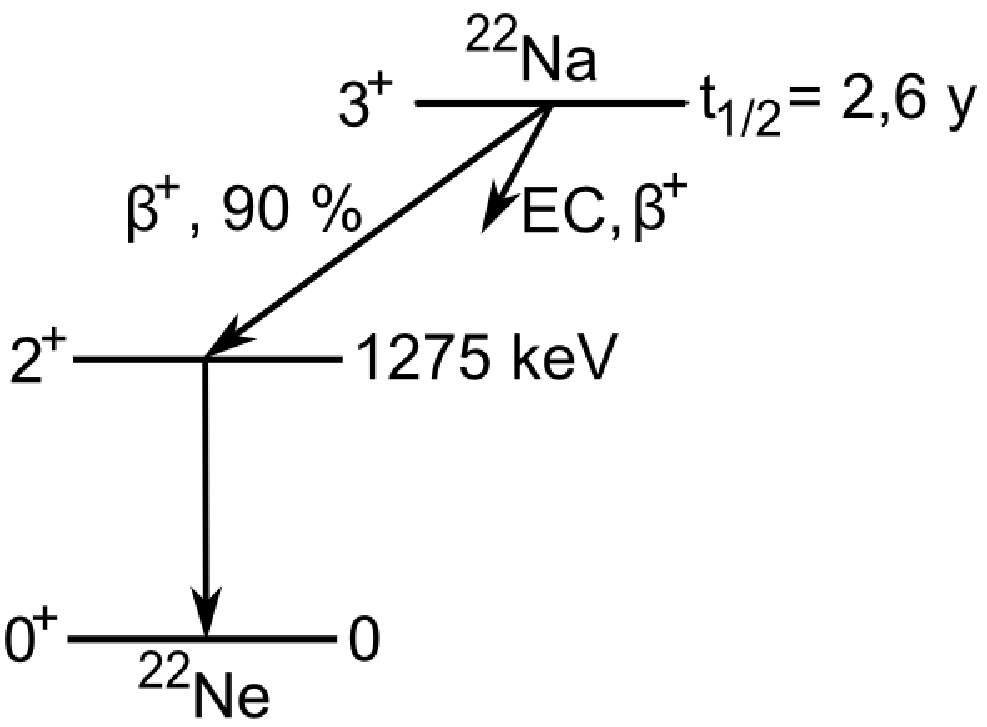
\includegraphics[width=0.5\textwidth]{graphics/natrium}
  \caption{Zerfallsschema von \Na~\cite{skript}}
  \label{fig:natrium}
\end{figure}
If a positron anihilates, two $\unit[511]{keV}$-photons are created. The detection of one of these stops the measurement.

\section{Experimental Setup}

\section{Experimentation and Analysis}
\subsection{Spectra}\label{subsec:ana_spectra}
First, we want to record the \Na spectrum with both scintillation detectors. In order to do this we set up the experiment as shown in figure \ref{fig:setup_prompt}.
\begin{figure}[H]
  \resizebox{0.4\textwidth}{!}{
    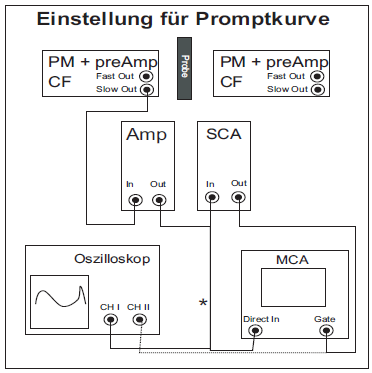
\includegraphics{graphics/setup_prompt}
}
  \caption{Set up for measuring the spectra and performing the adjustment for prompt curve measurement and the time calibration. This set up is used for each detector separately. '*' marks the position of an additional delay.}
  \label{fig:setup_prompt}
\end{figure}
Before measuring the spectra we connect the SCA's and the amplifier's output to an oscilloscope to check if the amplifier's signal is inside the gate signal. For adjustment we use the delay placed at '*'. The measured spectra are shown in figures \ref{fig:ana_spectrum_left} and \ref{fig:ana_spectrum_right}.
\begin{figure}[H]
\begin{floatrow}
\ffigbox[0.5\textwidth]{}
{
\resizebox{0.5\textwidth}{!}{
	\begin{tikzpicture}[gnuplot]
%% generated with GNUPLOT 4.4p0 (Lua 5.1.4; terminal rev. 97, script rev. 96a)
%% 18.04.2010 20:12:58
\gpcolor{gp lt color border}
\gpsetlinetype{gp lt border}
\gpsetlinewidth{1.00}
\draw[gp path] (1.872,0.985)--(2.052,0.985);
\draw[gp path] (12.039,0.985)--(11.859,0.985);
\node[gp node right] at (1.688,0.985) { 0};
\draw[gp path] (1.872,2.042)--(2.052,2.042);
\draw[gp path] (12.039,2.042)--(11.859,2.042);
\node[gp node right] at (1.688,2.042) { 1000};
\draw[gp path] (1.872,3.098)--(2.052,3.098);
\draw[gp path] (12.039,3.098)--(11.859,3.098);
\node[gp node right] at (1.688,3.098) { 2000};
\draw[gp path] (1.872,4.155)--(2.052,4.155);
\draw[gp path] (12.039,4.155)--(11.859,4.155);
\node[gp node right] at (1.688,4.155) { 3000};
\draw[gp path] (1.872,5.211)--(2.052,5.211);
\draw[gp path] (12.039,5.211)--(11.859,5.211);
\node[gp node right] at (1.688,5.211) { 4000};
\draw[gp path] (1.872,6.268)--(2.052,6.268);
\draw[gp path] (12.039,6.268)--(11.859,6.268);
\node[gp node right] at (1.688,6.268) { 5000};
\draw[gp path] (1.872,7.324)--(2.052,7.324);
\draw[gp path] (12.039,7.324)--(11.859,7.324);
\node[gp node right] at (1.688,7.324) { 6000};
\draw[gp path] (1.872,8.381)--(2.052,8.381);
\draw[gp path] (12.039,8.381)--(11.859,8.381);
\node[gp node right] at (1.688,8.381) { 7000};
\draw[gp path] (1.872,0.985)--(1.872,1.165);
\draw[gp path] (1.872,8.381)--(1.872,8.201);
\node[gp node center] at (1.872,0.677) { 0};
\draw[gp path] (3.905,0.985)--(3.905,1.165);
\draw[gp path] (3.905,8.381)--(3.905,8.201);
\node[gp node center] at (3.905,0.677) { 1000};
\draw[gp path] (5.939,0.985)--(5.939,1.165);
\draw[gp path] (5.939,8.381)--(5.939,8.201);
\node[gp node center] at (5.939,0.677) { 2000};
\draw[gp path] (7.972,0.985)--(7.972,1.165);
\draw[gp path] (7.972,8.381)--(7.972,8.201);
\node[gp node center] at (7.972,0.677) { 3000};
\draw[gp path] (10.006,0.985)--(10.006,1.165);
\draw[gp path] (10.006,8.381)--(10.006,8.201);
\node[gp node center] at (10.006,0.677) { 4000};
\draw[gp path] (12.039,0.985)--(12.039,1.165);
\draw[gp path] (12.039,8.381)--(12.039,8.201);
\node[gp node center] at (12.039,0.677) { 5000};
\draw[gp path] (1.872,8.381)--(1.872,0.985)--(12.039,0.985)--(12.039,8.381)--cycle;
\node[gp node center,rotate=-270] at (0.430,4.683) {Count};
\node[gp node center] at (6.955,0.215) {Channel};
\node[gp node right] at (10.571,8.047) {Data};
\gpcolor{gp lt color 0}
\gpsetpointsize{1.20}
\gppoint{gp mark 7}{(1.872,0.985)}
\gppoint{gp mark 7}{(1.874,0.985)}
\gppoint{gp mark 7}{(1.876,0.985)}
\gppoint{gp mark 7}{(1.878,0.985)}
\gppoint{gp mark 7}{(1.880,0.985)}
\gppoint{gp mark 7}{(1.882,0.985)}
\gppoint{gp mark 7}{(1.884,0.985)}
\gppoint{gp mark 7}{(1.886,0.985)}
\gppoint{gp mark 7}{(1.888,0.985)}
\gppoint{gp mark 7}{(1.890,0.985)}
\gppoint{gp mark 7}{(1.892,0.985)}
\gppoint{gp mark 7}{(1.894,0.985)}
\gppoint{gp mark 7}{(1.896,0.985)}
\gppoint{gp mark 7}{(1.898,0.985)}
\gppoint{gp mark 7}{(1.900,0.985)}
\gppoint{gp mark 7}{(1.903,0.985)}
\gppoint{gp mark 7}{(1.905,0.985)}
\gppoint{gp mark 7}{(1.907,0.985)}
\gppoint{gp mark 7}{(1.909,0.985)}
\gppoint{gp mark 7}{(1.911,0.985)}
\gppoint{gp mark 7}{(1.913,0.986)}
\gppoint{gp mark 7}{(1.915,0.985)}
\gppoint{gp mark 7}{(1.917,0.985)}
\gppoint{gp mark 7}{(1.919,0.985)}
\gppoint{gp mark 7}{(1.921,0.985)}
\gppoint{gp mark 7}{(1.923,0.985)}
\gppoint{gp mark 7}{(1.925,0.985)}
\gppoint{gp mark 7}{(1.927,0.985)}
\gppoint{gp mark 7}{(1.929,0.987)}
\gppoint{gp mark 7}{(1.931,0.987)}
\gppoint{gp mark 7}{(1.933,1.007)}
\gppoint{gp mark 7}{(1.935,1.120)}
\gppoint{gp mark 7}{(1.937,1.310)}
\gppoint{gp mark 7}{(1.939,1.594)}
\gppoint{gp mark 7}{(1.941,1.937)}
\gppoint{gp mark 7}{(1.943,2.369)}
\gppoint{gp mark 7}{(1.945,2.763)}
\gppoint{gp mark 7}{(1.947,2.904)}
\gppoint{gp mark 7}{(1.949,3.038)}
\gppoint{gp mark 7}{(1.951,3.050)}
\gppoint{gp mark 7}{(1.953,2.985)}
\gppoint{gp mark 7}{(1.955,3.043)}
\gppoint{gp mark 7}{(1.957,3.038)}
\gppoint{gp mark 7}{(1.959,3.031)}
\gppoint{gp mark 7}{(1.961,3.006)}
\gppoint{gp mark 7}{(1.964,3.121)}
\gppoint{gp mark 7}{(1.966,3.104)}
\gppoint{gp mark 7}{(1.968,3.035)}
\gppoint{gp mark 7}{(1.970,3.048)}
\gppoint{gp mark 7}{(1.972,3.060)}
\gppoint{gp mark 7}{(1.974,3.021)}
\gppoint{gp mark 7}{(1.976,3.185)}
\gppoint{gp mark 7}{(1.978,3.118)}
\gppoint{gp mark 7}{(1.980,3.117)}
\gppoint{gp mark 7}{(1.982,3.201)}
\gppoint{gp mark 7}{(1.984,3.177)}
\gppoint{gp mark 7}{(1.986,3.221)}
\gppoint{gp mark 7}{(1.988,3.196)}
\gppoint{gp mark 7}{(1.990,3.182)}
\gppoint{gp mark 7}{(1.992,3.216)}
\gppoint{gp mark 7}{(1.994,3.278)}
\gppoint{gp mark 7}{(1.996,3.201)}
\gppoint{gp mark 7}{(1.998,3.203)}
\gppoint{gp mark 7}{(2.000,3.258)}
\gppoint{gp mark 7}{(2.002,3.243)}
\gppoint{gp mark 7}{(2.004,3.260)}
\gppoint{gp mark 7}{(2.006,3.183)}
\gppoint{gp mark 7}{(2.008,3.253)}
\gppoint{gp mark 7}{(2.010,3.269)}
\gppoint{gp mark 7}{(2.012,3.258)}
\gppoint{gp mark 7}{(2.014,3.303)}
\gppoint{gp mark 7}{(2.016,3.281)}
\gppoint{gp mark 7}{(2.018,3.332)}
\gppoint{gp mark 7}{(2.020,3.290)}
\gppoint{gp mark 7}{(2.022,3.275)}
\gppoint{gp mark 7}{(2.025,3.368)}
\gppoint{gp mark 7}{(2.027,3.431)}
\gppoint{gp mark 7}{(2.029,3.353)}
\gppoint{gp mark 7}{(2.031,3.327)}
\gppoint{gp mark 7}{(2.033,3.335)}
\gppoint{gp mark 7}{(2.035,3.362)}
\gppoint{gp mark 7}{(2.037,3.423)}
\gppoint{gp mark 7}{(2.039,3.401)}
\gppoint{gp mark 7}{(2.041,3.367)}
\gppoint{gp mark 7}{(2.043,3.447)}
\gppoint{gp mark 7}{(2.045,3.432)}
\gppoint{gp mark 7}{(2.047,3.335)}
\gppoint{gp mark 7}{(2.049,3.421)}
\gppoint{gp mark 7}{(2.051,3.495)}
\gppoint{gp mark 7}{(2.053,3.510)}
\gppoint{gp mark 7}{(2.055,3.521)}
\gppoint{gp mark 7}{(2.057,3.467)}
\gppoint{gp mark 7}{(2.059,3.577)}
\gppoint{gp mark 7}{(2.061,3.397)}
\gppoint{gp mark 7}{(2.063,3.526)}
\gppoint{gp mark 7}{(2.065,3.529)}
\gppoint{gp mark 7}{(2.067,3.419)}
\gppoint{gp mark 7}{(2.069,3.474)}
\gppoint{gp mark 7}{(2.071,3.533)}
\gppoint{gp mark 7}{(2.073,3.528)}
\gppoint{gp mark 7}{(2.075,3.546)}
\gppoint{gp mark 7}{(2.077,3.511)}
\gppoint{gp mark 7}{(2.079,3.554)}
\gppoint{gp mark 7}{(2.081,3.531)}
\gppoint{gp mark 7}{(2.083,3.568)}
\gppoint{gp mark 7}{(2.086,3.596)}
\gppoint{gp mark 7}{(2.088,3.571)}
\gppoint{gp mark 7}{(2.090,3.587)}
\gppoint{gp mark 7}{(2.092,3.611)}
\gppoint{gp mark 7}{(2.094,3.654)}
\gppoint{gp mark 7}{(2.096,3.599)}
\gppoint{gp mark 7}{(2.098,3.597)}
\gppoint{gp mark 7}{(2.100,3.655)}
\gppoint{gp mark 7}{(2.102,3.678)}
\gppoint{gp mark 7}{(2.104,3.557)}
\gppoint{gp mark 7}{(2.106,3.689)}
\gppoint{gp mark 7}{(2.108,3.681)}
\gppoint{gp mark 7}{(2.110,3.720)}
\gppoint{gp mark 7}{(2.112,3.809)}
\gppoint{gp mark 7}{(2.114,3.708)}
\gppoint{gp mark 7}{(2.116,3.724)}
\gppoint{gp mark 7}{(2.118,3.770)}
\gppoint{gp mark 7}{(2.120,3.715)}
\gppoint{gp mark 7}{(2.122,3.741)}
\gppoint{gp mark 7}{(2.124,3.696)}
\gppoint{gp mark 7}{(2.126,3.776)}
\gppoint{gp mark 7}{(2.128,3.771)}
\gppoint{gp mark 7}{(2.130,3.912)}
\gppoint{gp mark 7}{(2.132,3.694)}
\gppoint{gp mark 7}{(2.134,3.727)}
\gppoint{gp mark 7}{(2.136,3.832)}
\gppoint{gp mark 7}{(2.138,3.724)}
\gppoint{gp mark 7}{(2.140,3.775)}
\gppoint{gp mark 7}{(2.142,3.884)}
\gppoint{gp mark 7}{(2.144,3.843)}
\gppoint{gp mark 7}{(2.147,3.753)}
\gppoint{gp mark 7}{(2.149,3.858)}
\gppoint{gp mark 7}{(2.151,3.845)}
\gppoint{gp mark 7}{(2.153,3.917)}
\gppoint{gp mark 7}{(2.155,3.817)}
\gppoint{gp mark 7}{(2.157,3.883)}
\gppoint{gp mark 7}{(2.159,4.023)}
\gppoint{gp mark 7}{(2.161,4.011)}
\gppoint{gp mark 7}{(2.163,3.949)}
\gppoint{gp mark 7}{(2.165,4.010)}
\gppoint{gp mark 7}{(2.167,3.989)}
\gppoint{gp mark 7}{(2.169,3.965)}
\gppoint{gp mark 7}{(2.171,3.912)}
\gppoint{gp mark 7}{(2.173,3.990)}
\gppoint{gp mark 7}{(2.175,3.940)}
\gppoint{gp mark 7}{(2.177,3.921)}
\gppoint{gp mark 7}{(2.179,4.035)}
\gppoint{gp mark 7}{(2.181,3.993)}
\gppoint{gp mark 7}{(2.183,4.111)}
\gppoint{gp mark 7}{(2.185,3.997)}
\gppoint{gp mark 7}{(2.187,4.000)}
\gppoint{gp mark 7}{(2.189,3.977)}
\gppoint{gp mark 7}{(2.191,3.944)}
\gppoint{gp mark 7}{(2.193,4.042)}
\gppoint{gp mark 7}{(2.195,4.027)}
\gppoint{gp mark 7}{(2.197,4.146)}
\gppoint{gp mark 7}{(2.199,4.056)}
\gppoint{gp mark 7}{(2.201,4.121)}
\gppoint{gp mark 7}{(2.203,4.045)}
\gppoint{gp mark 7}{(2.205,3.929)}
\gppoint{gp mark 7}{(2.208,4.103)}
\gppoint{gp mark 7}{(2.210,4.222)}
\gppoint{gp mark 7}{(2.212,4.214)}
\gppoint{gp mark 7}{(2.214,4.212)}
\gppoint{gp mark 7}{(2.216,4.224)}
\gppoint{gp mark 7}{(2.218,4.152)}
\gppoint{gp mark 7}{(2.220,4.256)}
\gppoint{gp mark 7}{(2.222,4.135)}
\gppoint{gp mark 7}{(2.224,4.237)}
\gppoint{gp mark 7}{(2.226,4.269)}
\gppoint{gp mark 7}{(2.228,4.099)}
\gppoint{gp mark 7}{(2.230,4.265)}
\gppoint{gp mark 7}{(2.232,4.190)}
\gppoint{gp mark 7}{(2.234,4.218)}
\gppoint{gp mark 7}{(2.236,4.339)}
\gppoint{gp mark 7}{(2.238,4.283)}
\gppoint{gp mark 7}{(2.240,4.437)}
\gppoint{gp mark 7}{(2.242,4.321)}
\gppoint{gp mark 7}{(2.244,4.221)}
\gppoint{gp mark 7}{(2.246,4.223)}
\gppoint{gp mark 7}{(2.248,4.250)}
\gppoint{gp mark 7}{(2.250,4.363)}
\gppoint{gp mark 7}{(2.252,4.301)}
\gppoint{gp mark 7}{(2.254,4.378)}
\gppoint{gp mark 7}{(2.256,4.417)}
\gppoint{gp mark 7}{(2.258,4.232)}
\gppoint{gp mark 7}{(2.260,4.472)}
\gppoint{gp mark 7}{(2.262,4.379)}
\gppoint{gp mark 7}{(2.264,4.365)}
\gppoint{gp mark 7}{(2.266,4.409)}
\gppoint{gp mark 7}{(2.269,4.423)}
\gppoint{gp mark 7}{(2.271,4.391)}
\gppoint{gp mark 7}{(2.273,4.405)}
\gppoint{gp mark 7}{(2.275,4.418)}
\gppoint{gp mark 7}{(2.277,4.503)}
\gppoint{gp mark 7}{(2.279,4.495)}
\gppoint{gp mark 7}{(2.281,4.546)}
\gppoint{gp mark 7}{(2.283,4.389)}
\gppoint{gp mark 7}{(2.285,4.448)}
\gppoint{gp mark 7}{(2.287,4.549)}
\gppoint{gp mark 7}{(2.289,4.475)}
\gppoint{gp mark 7}{(2.291,4.545)}
\gppoint{gp mark 7}{(2.293,4.522)}
\gppoint{gp mark 7}{(2.295,4.650)}
\gppoint{gp mark 7}{(2.297,4.641)}
\gppoint{gp mark 7}{(2.299,4.642)}
\gppoint{gp mark 7}{(2.301,4.508)}
\gppoint{gp mark 7}{(2.303,4.490)}
\gppoint{gp mark 7}{(2.305,4.559)}
\gppoint{gp mark 7}{(2.307,4.627)}
\gppoint{gp mark 7}{(2.309,4.652)}
\gppoint{gp mark 7}{(2.311,4.632)}
\gppoint{gp mark 7}{(2.313,4.642)}
\gppoint{gp mark 7}{(2.315,4.683)}
\gppoint{gp mark 7}{(2.317,4.679)}
\gppoint{gp mark 7}{(2.319,4.615)}
\gppoint{gp mark 7}{(2.321,4.702)}
\gppoint{gp mark 7}{(2.323,4.807)}
\gppoint{gp mark 7}{(2.325,4.728)}
\gppoint{gp mark 7}{(2.327,4.693)}
\gppoint{gp mark 7}{(2.330,4.870)}
\gppoint{gp mark 7}{(2.332,4.839)}
\gppoint{gp mark 7}{(2.334,4.792)}
\gppoint{gp mark 7}{(2.336,4.919)}
\gppoint{gp mark 7}{(2.338,4.957)}
\gppoint{gp mark 7}{(2.340,4.790)}
\gppoint{gp mark 7}{(2.342,4.938)}
\gppoint{gp mark 7}{(2.344,4.911)}
\gppoint{gp mark 7}{(2.346,4.870)}
\gppoint{gp mark 7}{(2.348,4.890)}
\gppoint{gp mark 7}{(2.350,4.952)}
\gppoint{gp mark 7}{(2.352,4.992)}
\gppoint{gp mark 7}{(2.354,4.857)}
\gppoint{gp mark 7}{(2.356,4.897)}
\gppoint{gp mark 7}{(2.358,4.876)}
\gppoint{gp mark 7}{(2.360,5.007)}
\gppoint{gp mark 7}{(2.362,5.109)}
\gppoint{gp mark 7}{(2.364,5.088)}
\gppoint{gp mark 7}{(2.366,5.133)}
\gppoint{gp mark 7}{(2.368,5.064)}
\gppoint{gp mark 7}{(2.370,5.052)}
\gppoint{gp mark 7}{(2.372,5.033)}
\gppoint{gp mark 7}{(2.374,5.090)}
\gppoint{gp mark 7}{(2.376,5.108)}
\gppoint{gp mark 7}{(2.378,5.073)}
\gppoint{gp mark 7}{(2.380,4.977)}
\gppoint{gp mark 7}{(2.382,5.167)}
\gppoint{gp mark 7}{(2.384,5.209)}
\gppoint{gp mark 7}{(2.386,5.124)}
\gppoint{gp mark 7}{(2.388,5.175)}
\gppoint{gp mark 7}{(2.391,5.208)}
\gppoint{gp mark 7}{(2.393,5.109)}
\gppoint{gp mark 7}{(2.395,5.054)}
\gppoint{gp mark 7}{(2.397,5.222)}
\gppoint{gp mark 7}{(2.399,5.068)}
\gppoint{gp mark 7}{(2.401,5.146)}
\gppoint{gp mark 7}{(2.403,5.317)}
\gppoint{gp mark 7}{(2.405,5.256)}
\gppoint{gp mark 7}{(2.407,5.380)}
\gppoint{gp mark 7}{(2.409,5.246)}
\gppoint{gp mark 7}{(2.411,5.294)}
\gppoint{gp mark 7}{(2.413,5.255)}
\gppoint{gp mark 7}{(2.415,5.241)}
\gppoint{gp mark 7}{(2.417,5.192)}
\gppoint{gp mark 7}{(2.419,5.138)}
\gppoint{gp mark 7}{(2.421,5.259)}
\gppoint{gp mark 7}{(2.423,5.153)}
\gppoint{gp mark 7}{(2.425,5.310)}
\gppoint{gp mark 7}{(2.427,5.151)}
\gppoint{gp mark 7}{(2.429,5.244)}
\gppoint{gp mark 7}{(2.431,5.311)}
\gppoint{gp mark 7}{(2.433,5.314)}
\gppoint{gp mark 7}{(2.435,5.252)}
\gppoint{gp mark 7}{(2.437,5.317)}
\gppoint{gp mark 7}{(2.439,5.382)}
\gppoint{gp mark 7}{(2.441,5.409)}
\gppoint{gp mark 7}{(2.443,5.333)}
\gppoint{gp mark 7}{(2.445,5.247)}
\gppoint{gp mark 7}{(2.447,5.257)}
\gppoint{gp mark 7}{(2.449,5.454)}
\gppoint{gp mark 7}{(2.452,5.280)}
\gppoint{gp mark 7}{(2.454,5.274)}
\gppoint{gp mark 7}{(2.456,5.432)}
\gppoint{gp mark 7}{(2.458,5.516)}
\gppoint{gp mark 7}{(2.460,5.350)}
\gppoint{gp mark 7}{(2.462,5.337)}
\gppoint{gp mark 7}{(2.464,5.391)}
\gppoint{gp mark 7}{(2.466,5.431)}
\gppoint{gp mark 7}{(2.468,5.349)}
\gppoint{gp mark 7}{(2.470,5.371)}
\gppoint{gp mark 7}{(2.472,5.331)}
\gppoint{gp mark 7}{(2.474,5.345)}
\gppoint{gp mark 7}{(2.476,5.465)}
\gppoint{gp mark 7}{(2.478,5.389)}
\gppoint{gp mark 7}{(2.480,5.443)}
\gppoint{gp mark 7}{(2.482,5.534)}
\gppoint{gp mark 7}{(2.484,5.585)}
\gppoint{gp mark 7}{(2.486,5.600)}
\gppoint{gp mark 7}{(2.488,5.563)}
\gppoint{gp mark 7}{(2.490,5.553)}
\gppoint{gp mark 7}{(2.492,5.509)}
\gppoint{gp mark 7}{(2.494,5.588)}
\gppoint{gp mark 7}{(2.496,5.549)}
\gppoint{gp mark 7}{(2.498,5.580)}
\gppoint{gp mark 7}{(2.500,5.513)}
\gppoint{gp mark 7}{(2.502,5.650)}
\gppoint{gp mark 7}{(2.504,5.670)}
\gppoint{gp mark 7}{(2.506,5.541)}
\gppoint{gp mark 7}{(2.508,5.635)}
\gppoint{gp mark 7}{(2.510,5.696)}
\gppoint{gp mark 7}{(2.513,5.746)}
\gppoint{gp mark 7}{(2.515,5.690)}
\gppoint{gp mark 7}{(2.517,5.604)}
\gppoint{gp mark 7}{(2.519,5.684)}
\gppoint{gp mark 7}{(2.521,5.555)}
\gppoint{gp mark 7}{(2.523,5.705)}
\gppoint{gp mark 7}{(2.525,5.573)}
\gppoint{gp mark 7}{(2.527,5.541)}
\gppoint{gp mark 7}{(2.529,5.677)}
\gppoint{gp mark 7}{(2.531,5.716)}
\gppoint{gp mark 7}{(2.533,5.603)}
\gppoint{gp mark 7}{(2.535,5.749)}
\gppoint{gp mark 7}{(2.537,5.691)}
\gppoint{gp mark 7}{(2.539,5.599)}
\gppoint{gp mark 7}{(2.541,5.671)}
\gppoint{gp mark 7}{(2.543,5.769)}
\gppoint{gp mark 7}{(2.545,5.742)}
\gppoint{gp mark 7}{(2.547,5.805)}
\gppoint{gp mark 7}{(2.549,5.669)}
\gppoint{gp mark 7}{(2.551,5.727)}
\gppoint{gp mark 7}{(2.553,5.538)}
\gppoint{gp mark 7}{(2.555,5.886)}
\gppoint{gp mark 7}{(2.557,5.801)}
\gppoint{gp mark 7}{(2.559,5.715)}
\gppoint{gp mark 7}{(2.561,5.778)}
\gppoint{gp mark 7}{(2.563,5.803)}
\gppoint{gp mark 7}{(2.565,5.709)}
\gppoint{gp mark 7}{(2.567,5.809)}
\gppoint{gp mark 7}{(2.569,5.889)}
\gppoint{gp mark 7}{(2.571,5.823)}
\gppoint{gp mark 7}{(2.574,5.868)}
\gppoint{gp mark 7}{(2.576,5.809)}
\gppoint{gp mark 7}{(2.578,5.831)}
\gppoint{gp mark 7}{(2.580,5.772)}
\gppoint{gp mark 7}{(2.582,5.862)}
\gppoint{gp mark 7}{(2.584,5.779)}
\gppoint{gp mark 7}{(2.586,5.960)}
\gppoint{gp mark 7}{(2.588,5.907)}
\gppoint{gp mark 7}{(2.590,5.956)}
\gppoint{gp mark 7}{(2.592,5.848)}
\gppoint{gp mark 7}{(2.594,6.008)}
\gppoint{gp mark 7}{(2.596,5.831)}
\gppoint{gp mark 7}{(2.598,6.023)}
\gppoint{gp mark 7}{(2.600,5.958)}
\gppoint{gp mark 7}{(2.602,5.940)}
\gppoint{gp mark 7}{(2.604,5.967)}
\gppoint{gp mark 7}{(2.606,5.985)}
\gppoint{gp mark 7}{(2.608,5.878)}
\gppoint{gp mark 7}{(2.610,5.960)}
\gppoint{gp mark 7}{(2.612,5.939)}
\gppoint{gp mark 7}{(2.614,5.865)}
\gppoint{gp mark 7}{(2.616,5.945)}
\gppoint{gp mark 7}{(2.618,5.915)}
\gppoint{gp mark 7}{(2.620,5.940)}
\gppoint{gp mark 7}{(2.622,5.863)}
\gppoint{gp mark 7}{(2.624,5.963)}
\gppoint{gp mark 7}{(2.626,5.882)}
\gppoint{gp mark 7}{(2.628,6.019)}
\gppoint{gp mark 7}{(2.630,5.934)}
\gppoint{gp mark 7}{(2.632,5.930)}
\gppoint{gp mark 7}{(2.635,5.965)}
\gppoint{gp mark 7}{(2.637,6.020)}
\gppoint{gp mark 7}{(2.639,6.061)}
\gppoint{gp mark 7}{(2.641,6.127)}
\gppoint{gp mark 7}{(2.643,5.922)}
\gppoint{gp mark 7}{(2.645,6.091)}
\gppoint{gp mark 7}{(2.647,5.956)}
\gppoint{gp mark 7}{(2.649,5.964)}
\gppoint{gp mark 7}{(2.651,5.963)}
\gppoint{gp mark 7}{(2.653,6.045)}
\gppoint{gp mark 7}{(2.655,5.957)}
\gppoint{gp mark 7}{(2.657,6.078)}
\gppoint{gp mark 7}{(2.659,5.880)}
\gppoint{gp mark 7}{(2.661,6.076)}
\gppoint{gp mark 7}{(2.663,6.120)}
\gppoint{gp mark 7}{(2.665,6.053)}
\gppoint{gp mark 7}{(2.667,6.069)}
\gppoint{gp mark 7}{(2.669,6.078)}
\gppoint{gp mark 7}{(2.671,6.031)}
\gppoint{gp mark 7}{(2.673,6.126)}
\gppoint{gp mark 7}{(2.675,6.029)}
\gppoint{gp mark 7}{(2.677,6.041)}
\gppoint{gp mark 7}{(2.679,6.075)}
\gppoint{gp mark 7}{(2.681,5.818)}
\gppoint{gp mark 7}{(2.683,5.895)}
\gppoint{gp mark 7}{(2.685,6.220)}
\gppoint{gp mark 7}{(2.687,5.941)}
\gppoint{gp mark 7}{(2.689,6.011)}
\gppoint{gp mark 7}{(2.691,6.126)}
\gppoint{gp mark 7}{(2.693,6.069)}
\gppoint{gp mark 7}{(2.696,6.083)}
\gppoint{gp mark 7}{(2.698,6.085)}
\gppoint{gp mark 7}{(2.700,6.027)}
\gppoint{gp mark 7}{(2.702,6.076)}
\gppoint{gp mark 7}{(2.704,6.065)}
\gppoint{gp mark 7}{(2.706,5.966)}
\gppoint{gp mark 7}{(2.708,6.001)}
\gppoint{gp mark 7}{(2.710,6.051)}
\gppoint{gp mark 7}{(2.712,5.986)}
\gppoint{gp mark 7}{(2.714,6.068)}
\gppoint{gp mark 7}{(2.716,6.172)}
\gppoint{gp mark 7}{(2.718,6.193)}
\gppoint{gp mark 7}{(2.720,6.158)}
\gppoint{gp mark 7}{(2.722,5.991)}
\gppoint{gp mark 7}{(2.724,6.090)}
\gppoint{gp mark 7}{(2.726,6.282)}
\gppoint{gp mark 7}{(2.728,6.127)}
\gppoint{gp mark 7}{(2.730,6.030)}
\gppoint{gp mark 7}{(2.732,6.058)}
\gppoint{gp mark 7}{(2.734,6.132)}
\gppoint{gp mark 7}{(2.736,6.223)}
\gppoint{gp mark 7}{(2.738,6.041)}
\gppoint{gp mark 7}{(2.740,6.017)}
\gppoint{gp mark 7}{(2.742,6.104)}
\gppoint{gp mark 7}{(2.744,6.183)}
\gppoint{gp mark 7}{(2.746,6.139)}
\gppoint{gp mark 7}{(2.748,6.069)}
\gppoint{gp mark 7}{(2.750,6.257)}
\gppoint{gp mark 7}{(2.752,6.124)}
\gppoint{gp mark 7}{(2.754,6.048)}
\gppoint{gp mark 7}{(2.757,6.229)}
\gppoint{gp mark 7}{(2.759,6.121)}
\gppoint{gp mark 7}{(2.761,6.100)}
\gppoint{gp mark 7}{(2.763,6.247)}
\gppoint{gp mark 7}{(2.765,6.167)}
\gppoint{gp mark 7}{(2.767,6.170)}
\gppoint{gp mark 7}{(2.769,6.061)}
\gppoint{gp mark 7}{(2.771,6.134)}
\gppoint{gp mark 7}{(2.773,5.986)}
\gppoint{gp mark 7}{(2.775,6.285)}
\gppoint{gp mark 7}{(2.777,5.961)}
\gppoint{gp mark 7}{(2.779,6.090)}
\gppoint{gp mark 7}{(2.781,6.055)}
\gppoint{gp mark 7}{(2.783,6.095)}
\gppoint{gp mark 7}{(2.785,6.015)}
\gppoint{gp mark 7}{(2.787,6.024)}
\gppoint{gp mark 7}{(2.789,6.217)}
\gppoint{gp mark 7}{(2.791,6.226)}
\gppoint{gp mark 7}{(2.793,6.057)}
\gppoint{gp mark 7}{(2.795,6.123)}
\gppoint{gp mark 7}{(2.797,6.108)}
\gppoint{gp mark 7}{(2.799,6.051)}
\gppoint{gp mark 7}{(2.801,6.036)}
\gppoint{gp mark 7}{(2.803,6.082)}
\gppoint{gp mark 7}{(2.805,5.998)}
\gppoint{gp mark 7}{(2.807,6.052)}
\gppoint{gp mark 7}{(2.809,6.002)}
\gppoint{gp mark 7}{(2.811,6.045)}
\gppoint{gp mark 7}{(2.813,6.108)}
\gppoint{gp mark 7}{(2.815,6.043)}
\gppoint{gp mark 7}{(2.818,5.931)}
\gppoint{gp mark 7}{(2.820,5.983)}
\gppoint{gp mark 7}{(2.822,6.031)}
\gppoint{gp mark 7}{(2.824,6.101)}
\gppoint{gp mark 7}{(2.826,6.058)}
\gppoint{gp mark 7}{(2.828,6.136)}
\gppoint{gp mark 7}{(2.830,6.125)}
\gppoint{gp mark 7}{(2.832,5.982)}
\gppoint{gp mark 7}{(2.834,6.028)}
\gppoint{gp mark 7}{(2.836,6.197)}
\gppoint{gp mark 7}{(2.838,6.144)}
\gppoint{gp mark 7}{(2.840,5.997)}
\gppoint{gp mark 7}{(2.842,5.968)}
\gppoint{gp mark 7}{(2.844,6.010)}
\gppoint{gp mark 7}{(2.846,5.968)}
\gppoint{gp mark 7}{(2.848,6.101)}
\gppoint{gp mark 7}{(2.850,6.016)}
\gppoint{gp mark 7}{(2.852,5.973)}
\gppoint{gp mark 7}{(2.854,6.063)}
\gppoint{gp mark 7}{(2.856,6.126)}
\gppoint{gp mark 7}{(2.858,5.851)}
\gppoint{gp mark 7}{(2.860,6.166)}
\gppoint{gp mark 7}{(2.862,6.096)}
\gppoint{gp mark 7}{(2.864,5.980)}
\gppoint{gp mark 7}{(2.866,5.968)}
\gppoint{gp mark 7}{(2.868,5.943)}
\gppoint{gp mark 7}{(2.870,6.008)}
\gppoint{gp mark 7}{(2.872,6.032)}
\gppoint{gp mark 7}{(2.874,6.044)}
\gppoint{gp mark 7}{(2.876,5.934)}
\gppoint{gp mark 7}{(2.879,6.004)}
\gppoint{gp mark 7}{(2.881,5.853)}
\gppoint{gp mark 7}{(2.883,5.845)}
\gppoint{gp mark 7}{(2.885,5.980)}
\gppoint{gp mark 7}{(2.887,5.876)}
\gppoint{gp mark 7}{(2.889,5.797)}
\gppoint{gp mark 7}{(2.891,5.965)}
\gppoint{gp mark 7}{(2.893,5.913)}
\gppoint{gp mark 7}{(2.895,6.061)}
\gppoint{gp mark 7}{(2.897,6.003)}
\gppoint{gp mark 7}{(2.899,5.881)}
\gppoint{gp mark 7}{(2.901,5.940)}
\gppoint{gp mark 7}{(2.903,6.061)}
\gppoint{gp mark 7}{(2.905,6.015)}
\gppoint{gp mark 7}{(2.907,5.862)}
\gppoint{gp mark 7}{(2.909,5.936)}
\gppoint{gp mark 7}{(2.911,5.873)}
\gppoint{gp mark 7}{(2.913,6.013)}
\gppoint{gp mark 7}{(2.915,5.887)}
\gppoint{gp mark 7}{(2.917,5.940)}
\gppoint{gp mark 7}{(2.919,5.975)}
\gppoint{gp mark 7}{(2.921,5.891)}
\gppoint{gp mark 7}{(2.923,5.894)}
\gppoint{gp mark 7}{(2.925,5.833)}
\gppoint{gp mark 7}{(2.927,5.898)}
\gppoint{gp mark 7}{(2.929,5.899)}
\gppoint{gp mark 7}{(2.931,5.895)}
\gppoint{gp mark 7}{(2.933,5.916)}
\gppoint{gp mark 7}{(2.935,5.896)}
\gppoint{gp mark 7}{(2.938,5.949)}
\gppoint{gp mark 7}{(2.940,5.892)}
\gppoint{gp mark 7}{(2.942,5.773)}
\gppoint{gp mark 7}{(2.944,5.882)}
\gppoint{gp mark 7}{(2.946,5.840)}
\gppoint{gp mark 7}{(2.948,5.837)}
\gppoint{gp mark 7}{(2.950,5.950)}
\gppoint{gp mark 7}{(2.952,5.916)}
\gppoint{gp mark 7}{(2.954,5.903)}
\gppoint{gp mark 7}{(2.956,5.834)}
\gppoint{gp mark 7}{(2.958,5.915)}
\gppoint{gp mark 7}{(2.960,5.648)}
\gppoint{gp mark 7}{(2.962,5.875)}
\gppoint{gp mark 7}{(2.964,5.804)}
\gppoint{gp mark 7}{(2.966,5.861)}
\gppoint{gp mark 7}{(2.968,5.772)}
\gppoint{gp mark 7}{(2.970,5.666)}
\gppoint{gp mark 7}{(2.972,5.771)}
\gppoint{gp mark 7}{(2.974,5.878)}
\gppoint{gp mark 7}{(2.976,5.732)}
\gppoint{gp mark 7}{(2.978,5.838)}
\gppoint{gp mark 7}{(2.980,5.879)}
\gppoint{gp mark 7}{(2.982,5.790)}
\gppoint{gp mark 7}{(2.984,5.804)}
\gppoint{gp mark 7}{(2.986,5.755)}
\gppoint{gp mark 7}{(2.988,5.739)}
\gppoint{gp mark 7}{(2.990,5.743)}
\gppoint{gp mark 7}{(2.992,5.817)}
\gppoint{gp mark 7}{(2.994,5.721)}
\gppoint{gp mark 7}{(2.996,5.640)}
\gppoint{gp mark 7}{(2.999,5.657)}
\gppoint{gp mark 7}{(3.001,5.662)}
\gppoint{gp mark 7}{(3.003,5.657)}
\gppoint{gp mark 7}{(3.005,5.678)}
\gppoint{gp mark 7}{(3.007,5.724)}
\gppoint{gp mark 7}{(3.009,5.607)}
\gppoint{gp mark 7}{(3.011,5.710)}
\gppoint{gp mark 7}{(3.013,5.727)}
\gppoint{gp mark 7}{(3.015,5.581)}
\gppoint{gp mark 7}{(3.017,5.710)}
\gppoint{gp mark 7}{(3.019,5.697)}
\gppoint{gp mark 7}{(3.021,5.714)}
\gppoint{gp mark 7}{(3.023,5.641)}
\gppoint{gp mark 7}{(3.025,5.630)}
\gppoint{gp mark 7}{(3.027,5.646)}
\gppoint{gp mark 7}{(3.029,5.618)}
\gppoint{gp mark 7}{(3.031,5.606)}
\gppoint{gp mark 7}{(3.033,5.696)}
\gppoint{gp mark 7}{(3.035,5.674)}
\gppoint{gp mark 7}{(3.037,5.617)}
\gppoint{gp mark 7}{(3.039,5.653)}
\gppoint{gp mark 7}{(3.041,5.807)}
\gppoint{gp mark 7}{(3.043,5.650)}
\gppoint{gp mark 7}{(3.045,5.604)}
\gppoint{gp mark 7}{(3.047,5.519)}
\gppoint{gp mark 7}{(3.049,5.457)}
\gppoint{gp mark 7}{(3.051,5.567)}
\gppoint{gp mark 7}{(3.053,5.565)}
\gppoint{gp mark 7}{(3.055,5.581)}
\gppoint{gp mark 7}{(3.057,5.613)}
\gppoint{gp mark 7}{(3.060,5.642)}
\gppoint{gp mark 7}{(3.062,5.668)}
\gppoint{gp mark 7}{(3.064,5.524)}
\gppoint{gp mark 7}{(3.066,5.605)}
\gppoint{gp mark 7}{(3.068,5.588)}
\gppoint{gp mark 7}{(3.070,5.669)}
\gppoint{gp mark 7}{(3.072,5.598)}
\gppoint{gp mark 7}{(3.074,5.568)}
\gppoint{gp mark 7}{(3.076,5.511)}
\gppoint{gp mark 7}{(3.078,5.483)}
\gppoint{gp mark 7}{(3.080,5.483)}
\gppoint{gp mark 7}{(3.082,5.584)}
\gppoint{gp mark 7}{(3.084,5.515)}
\gppoint{gp mark 7}{(3.086,5.483)}
\gppoint{gp mark 7}{(3.088,5.521)}
\gppoint{gp mark 7}{(3.090,5.509)}
\gppoint{gp mark 7}{(3.092,5.517)}
\gppoint{gp mark 7}{(3.094,5.485)}
\gppoint{gp mark 7}{(3.096,5.414)}
\gppoint{gp mark 7}{(3.098,5.572)}
\gppoint{gp mark 7}{(3.100,5.464)}
\gppoint{gp mark 7}{(3.102,5.427)}
\gppoint{gp mark 7}{(3.104,5.489)}
\gppoint{gp mark 7}{(3.106,5.440)}
\gppoint{gp mark 7}{(3.108,5.374)}
\gppoint{gp mark 7}{(3.110,5.459)}
\gppoint{gp mark 7}{(3.112,5.506)}
\gppoint{gp mark 7}{(3.114,5.348)}
\gppoint{gp mark 7}{(3.116,5.460)}
\gppoint{gp mark 7}{(3.118,5.360)}
\gppoint{gp mark 7}{(3.121,5.351)}
\gppoint{gp mark 7}{(3.123,5.387)}
\gppoint{gp mark 7}{(3.125,5.493)}
\gppoint{gp mark 7}{(3.127,5.242)}
\gppoint{gp mark 7}{(3.129,5.316)}
\gppoint{gp mark 7}{(3.131,5.349)}
\gppoint{gp mark 7}{(3.133,5.381)}
\gppoint{gp mark 7}{(3.135,5.286)}
\gppoint{gp mark 7}{(3.137,5.226)}
\gppoint{gp mark 7}{(3.139,5.408)}
\gppoint{gp mark 7}{(3.141,5.440)}
\gppoint{gp mark 7}{(3.143,5.319)}
\gppoint{gp mark 7}{(3.145,5.354)}
\gppoint{gp mark 7}{(3.147,5.276)}
\gppoint{gp mark 7}{(3.149,5.418)}
\gppoint{gp mark 7}{(3.151,5.517)}
\gppoint{gp mark 7}{(3.153,5.273)}
\gppoint{gp mark 7}{(3.155,5.340)}
\gppoint{gp mark 7}{(3.157,5.400)}
\gppoint{gp mark 7}{(3.159,5.306)}
\gppoint{gp mark 7}{(3.161,5.303)}
\gppoint{gp mark 7}{(3.163,5.300)}
\gppoint{gp mark 7}{(3.165,5.154)}
\gppoint{gp mark 7}{(3.167,5.239)}
\gppoint{gp mark 7}{(3.169,5.209)}
\gppoint{gp mark 7}{(3.171,5.184)}
\gppoint{gp mark 7}{(3.173,5.307)}
\gppoint{gp mark 7}{(3.175,5.286)}
\gppoint{gp mark 7}{(3.177,5.338)}
\gppoint{gp mark 7}{(3.179,5.283)}
\gppoint{gp mark 7}{(3.182,5.302)}
\gppoint{gp mark 7}{(3.184,5.299)}
\gppoint{gp mark 7}{(3.186,5.250)}
\gppoint{gp mark 7}{(3.188,5.229)}
\gppoint{gp mark 7}{(3.190,5.251)}
\gppoint{gp mark 7}{(3.192,5.179)}
\gppoint{gp mark 7}{(3.194,5.291)}
\gppoint{gp mark 7}{(3.196,5.252)}
\gppoint{gp mark 7}{(3.198,5.153)}
\gppoint{gp mark 7}{(3.200,5.210)}
\gppoint{gp mark 7}{(3.202,5.114)}
\gppoint{gp mark 7}{(3.204,5.313)}
\gppoint{gp mark 7}{(3.206,5.117)}
\gppoint{gp mark 7}{(3.208,5.137)}
\gppoint{gp mark 7}{(3.210,5.027)}
\gppoint{gp mark 7}{(3.212,5.132)}
\gppoint{gp mark 7}{(3.214,5.241)}
\gppoint{gp mark 7}{(3.216,5.063)}
\gppoint{gp mark 7}{(3.218,5.146)}
\gppoint{gp mark 7}{(3.220,5.127)}
\gppoint{gp mark 7}{(3.222,5.114)}
\gppoint{gp mark 7}{(3.224,5.031)}
\gppoint{gp mark 7}{(3.226,5.286)}
\gppoint{gp mark 7}{(3.228,5.094)}
\gppoint{gp mark 7}{(3.230,5.041)}
\gppoint{gp mark 7}{(3.232,5.096)}
\gppoint{gp mark 7}{(3.234,4.955)}
\gppoint{gp mark 7}{(3.236,5.097)}
\gppoint{gp mark 7}{(3.238,5.079)}
\gppoint{gp mark 7}{(3.240,5.027)}
\gppoint{gp mark 7}{(3.243,4.986)}
\gppoint{gp mark 7}{(3.245,4.983)}
\gppoint{gp mark 7}{(3.247,5.025)}
\gppoint{gp mark 7}{(3.249,5.106)}
\gppoint{gp mark 7}{(3.251,5.024)}
\gppoint{gp mark 7}{(3.253,4.999)}
\gppoint{gp mark 7}{(3.255,5.080)}
\gppoint{gp mark 7}{(3.257,5.056)}
\gppoint{gp mark 7}{(3.259,5.044)}
\gppoint{gp mark 7}{(3.261,5.041)}
\gppoint{gp mark 7}{(3.263,4.979)}
\gppoint{gp mark 7}{(3.265,5.006)}
\gppoint{gp mark 7}{(3.267,4.901)}
\gppoint{gp mark 7}{(3.269,5.056)}
\gppoint{gp mark 7}{(3.271,5.111)}
\gppoint{gp mark 7}{(3.273,4.975)}
\gppoint{gp mark 7}{(3.275,4.963)}
\gppoint{gp mark 7}{(3.277,4.910)}
\gppoint{gp mark 7}{(3.279,4.907)}
\gppoint{gp mark 7}{(3.281,5.026)}
\gppoint{gp mark 7}{(3.283,4.959)}
\gppoint{gp mark 7}{(3.285,5.044)}
\gppoint{gp mark 7}{(3.287,4.899)}
\gppoint{gp mark 7}{(3.289,5.111)}
\gppoint{gp mark 7}{(3.291,5.013)}
\gppoint{gp mark 7}{(3.293,4.931)}
\gppoint{gp mark 7}{(3.295,4.890)}
\gppoint{gp mark 7}{(3.297,4.929)}
\gppoint{gp mark 7}{(3.299,5.025)}
\gppoint{gp mark 7}{(3.301,4.950)}
\gppoint{gp mark 7}{(3.304,4.875)}
\gppoint{gp mark 7}{(3.306,4.949)}
\gppoint{gp mark 7}{(3.308,4.947)}
\gppoint{gp mark 7}{(3.310,5.065)}
\gppoint{gp mark 7}{(3.312,4.985)}
\gppoint{gp mark 7}{(3.314,4.803)}
\gppoint{gp mark 7}{(3.316,4.930)}
\gppoint{gp mark 7}{(3.318,4.859)}
\gppoint{gp mark 7}{(3.320,4.795)}
\gppoint{gp mark 7}{(3.322,4.849)}
\gppoint{gp mark 7}{(3.324,4.951)}
\gppoint{gp mark 7}{(3.326,4.914)}
\gppoint{gp mark 7}{(3.328,4.900)}
\gppoint{gp mark 7}{(3.330,4.846)}
\gppoint{gp mark 7}{(3.332,4.848)}
\gppoint{gp mark 7}{(3.334,4.798)}
\gppoint{gp mark 7}{(3.336,4.801)}
\gppoint{gp mark 7}{(3.338,4.833)}
\gppoint{gp mark 7}{(3.340,4.754)}
\gppoint{gp mark 7}{(3.342,4.907)}
\gppoint{gp mark 7}{(3.344,4.800)}
\gppoint{gp mark 7}{(3.346,4.801)}
\gppoint{gp mark 7}{(3.348,4.759)}
\gppoint{gp mark 7}{(3.350,4.801)}
\gppoint{gp mark 7}{(3.352,4.799)}
\gppoint{gp mark 7}{(3.354,4.899)}
\gppoint{gp mark 7}{(3.356,4.723)}
\gppoint{gp mark 7}{(3.358,4.656)}
\gppoint{gp mark 7}{(3.360,4.871)}
\gppoint{gp mark 7}{(3.362,4.663)}
\gppoint{gp mark 7}{(3.365,4.781)}
\gppoint{gp mark 7}{(3.367,4.911)}
\gppoint{gp mark 7}{(3.369,4.695)}
\gppoint{gp mark 7}{(3.371,4.849)}
\gppoint{gp mark 7}{(3.373,4.784)}
\gppoint{gp mark 7}{(3.375,4.544)}
\gppoint{gp mark 7}{(3.377,4.722)}
\gppoint{gp mark 7}{(3.379,4.662)}
\gppoint{gp mark 7}{(3.381,4.793)}
\gppoint{gp mark 7}{(3.383,4.728)}
\gppoint{gp mark 7}{(3.385,4.765)}
\gppoint{gp mark 7}{(3.387,4.709)}
\gppoint{gp mark 7}{(3.389,4.739)}
\gppoint{gp mark 7}{(3.391,4.649)}
\gppoint{gp mark 7}{(3.393,4.755)}
\gppoint{gp mark 7}{(3.395,4.704)}
\gppoint{gp mark 7}{(3.397,4.660)}
\gppoint{gp mark 7}{(3.399,4.679)}
\gppoint{gp mark 7}{(3.401,4.744)}
\gppoint{gp mark 7}{(3.403,4.755)}
\gppoint{gp mark 7}{(3.405,4.626)}
\gppoint{gp mark 7}{(3.407,4.691)}
\gppoint{gp mark 7}{(3.409,4.530)}
\gppoint{gp mark 7}{(3.411,4.613)}
\gppoint{gp mark 7}{(3.413,4.694)}
\gppoint{gp mark 7}{(3.415,4.698)}
\gppoint{gp mark 7}{(3.417,4.664)}
\gppoint{gp mark 7}{(3.419,4.722)}
\gppoint{gp mark 7}{(3.421,4.673)}
\gppoint{gp mark 7}{(3.423,4.621)}
\gppoint{gp mark 7}{(3.426,4.628)}
\gppoint{gp mark 7}{(3.428,4.590)}
\gppoint{gp mark 7}{(3.430,4.547)}
\gppoint{gp mark 7}{(3.432,4.662)}
\gppoint{gp mark 7}{(3.434,4.555)}
\gppoint{gp mark 7}{(3.436,4.469)}
\gppoint{gp mark 7}{(3.438,4.718)}
\gppoint{gp mark 7}{(3.440,4.584)}
\gppoint{gp mark 7}{(3.442,4.637)}
\gppoint{gp mark 7}{(3.444,4.619)}
\gppoint{gp mark 7}{(3.446,4.611)}
\gppoint{gp mark 7}{(3.448,4.483)}
\gppoint{gp mark 7}{(3.450,4.631)}
\gppoint{gp mark 7}{(3.452,4.585)}
\gppoint{gp mark 7}{(3.454,4.591)}
\gppoint{gp mark 7}{(3.456,4.577)}
\gppoint{gp mark 7}{(3.458,4.633)}
\gppoint{gp mark 7}{(3.460,4.555)}
\gppoint{gp mark 7}{(3.462,4.647)}
\gppoint{gp mark 7}{(3.464,4.589)}
\gppoint{gp mark 7}{(3.466,4.642)}
\gppoint{gp mark 7}{(3.468,4.478)}
\gppoint{gp mark 7}{(3.470,4.577)}
\gppoint{gp mark 7}{(3.472,4.621)}
\gppoint{gp mark 7}{(3.474,4.561)}
\gppoint{gp mark 7}{(3.476,4.485)}
\gppoint{gp mark 7}{(3.478,4.574)}
\gppoint{gp mark 7}{(3.480,4.520)}
\gppoint{gp mark 7}{(3.482,4.533)}
\gppoint{gp mark 7}{(3.484,4.470)}
\gppoint{gp mark 7}{(3.487,4.494)}
\gppoint{gp mark 7}{(3.489,4.347)}
\gppoint{gp mark 7}{(3.491,4.426)}
\gppoint{gp mark 7}{(3.493,4.475)}
\gppoint{gp mark 7}{(3.495,4.425)}
\gppoint{gp mark 7}{(3.497,4.502)}
\gppoint{gp mark 7}{(3.499,4.495)}
\gppoint{gp mark 7}{(3.501,4.395)}
\gppoint{gp mark 7}{(3.503,4.441)}
\gppoint{gp mark 7}{(3.505,4.459)}
\gppoint{gp mark 7}{(3.507,4.512)}
\gppoint{gp mark 7}{(3.509,4.479)}
\gppoint{gp mark 7}{(3.511,4.425)}
\gppoint{gp mark 7}{(3.513,4.477)}
\gppoint{gp mark 7}{(3.515,4.470)}
\gppoint{gp mark 7}{(3.517,4.413)}
\gppoint{gp mark 7}{(3.519,4.429)}
\gppoint{gp mark 7}{(3.521,4.534)}
\gppoint{gp mark 7}{(3.523,4.372)}
\gppoint{gp mark 7}{(3.525,4.348)}
\gppoint{gp mark 7}{(3.527,4.417)}
\gppoint{gp mark 7}{(3.529,4.355)}
\gppoint{gp mark 7}{(3.531,4.425)}
\gppoint{gp mark 7}{(3.533,4.500)}
\gppoint{gp mark 7}{(3.535,4.344)}
\gppoint{gp mark 7}{(3.537,4.465)}
\gppoint{gp mark 7}{(3.539,4.402)}
\gppoint{gp mark 7}{(3.541,4.275)}
\gppoint{gp mark 7}{(3.543,4.400)}
\gppoint{gp mark 7}{(3.545,4.484)}
\gppoint{gp mark 7}{(3.548,4.385)}
\gppoint{gp mark 7}{(3.550,4.326)}
\gppoint{gp mark 7}{(3.552,4.466)}
\gppoint{gp mark 7}{(3.554,4.382)}
\gppoint{gp mark 7}{(3.556,4.401)}
\gppoint{gp mark 7}{(3.558,4.382)}
\gppoint{gp mark 7}{(3.560,4.383)}
\gppoint{gp mark 7}{(3.562,4.329)}
\gppoint{gp mark 7}{(3.564,4.396)}
\gppoint{gp mark 7}{(3.566,4.352)}
\gppoint{gp mark 7}{(3.568,4.405)}
\gppoint{gp mark 7}{(3.570,4.335)}
\gppoint{gp mark 7}{(3.572,4.451)}
\gppoint{gp mark 7}{(3.574,4.388)}
\gppoint{gp mark 7}{(3.576,4.352)}
\gppoint{gp mark 7}{(3.578,4.275)}
\gppoint{gp mark 7}{(3.580,4.299)}
\gppoint{gp mark 7}{(3.582,4.411)}
\gppoint{gp mark 7}{(3.584,4.237)}
\gppoint{gp mark 7}{(3.586,4.293)}
\gppoint{gp mark 7}{(3.588,4.277)}
\gppoint{gp mark 7}{(3.590,4.334)}
\gppoint{gp mark 7}{(3.592,4.235)}
\gppoint{gp mark 7}{(3.594,4.398)}
\gppoint{gp mark 7}{(3.596,4.240)}
\gppoint{gp mark 7}{(3.598,4.268)}
\gppoint{gp mark 7}{(3.600,4.350)}
\gppoint{gp mark 7}{(3.602,4.308)}
\gppoint{gp mark 7}{(3.604,4.292)}
\gppoint{gp mark 7}{(3.606,4.312)}
\gppoint{gp mark 7}{(3.609,4.338)}
\gppoint{gp mark 7}{(3.611,4.261)}
\gppoint{gp mark 7}{(3.613,4.247)}
\gppoint{gp mark 7}{(3.615,4.309)}
\gppoint{gp mark 7}{(3.617,4.245)}
\gppoint{gp mark 7}{(3.619,4.274)}
\gppoint{gp mark 7}{(3.621,4.299)}
\gppoint{gp mark 7}{(3.623,4.192)}
\gppoint{gp mark 7}{(3.625,4.270)}
\gppoint{gp mark 7}{(3.627,4.267)}
\gppoint{gp mark 7}{(3.629,4.212)}
\gppoint{gp mark 7}{(3.631,4.254)}
\gppoint{gp mark 7}{(3.633,4.216)}
\gppoint{gp mark 7}{(3.635,4.308)}
\gppoint{gp mark 7}{(3.637,4.275)}
\gppoint{gp mark 7}{(3.639,4.346)}
\gppoint{gp mark 7}{(3.641,4.245)}
\gppoint{gp mark 7}{(3.643,4.232)}
\gppoint{gp mark 7}{(3.645,4.254)}
\gppoint{gp mark 7}{(3.647,4.280)}
\gppoint{gp mark 7}{(3.649,4.186)}
\gppoint{gp mark 7}{(3.651,4.274)}
\gppoint{gp mark 7}{(3.653,4.232)}
\gppoint{gp mark 7}{(3.655,4.278)}
\gppoint{gp mark 7}{(3.657,4.265)}
\gppoint{gp mark 7}{(3.659,4.228)}
\gppoint{gp mark 7}{(3.661,4.229)}
\gppoint{gp mark 7}{(3.663,4.133)}
\gppoint{gp mark 7}{(3.665,4.361)}
\gppoint{gp mark 7}{(3.667,4.267)}
\gppoint{gp mark 7}{(3.670,4.310)}
\gppoint{gp mark 7}{(3.672,4.215)}
\gppoint{gp mark 7}{(3.674,4.262)}
\gppoint{gp mark 7}{(3.676,4.193)}
\gppoint{gp mark 7}{(3.678,4.206)}
\gppoint{gp mark 7}{(3.680,4.218)}
\gppoint{gp mark 7}{(3.682,4.212)}
\gppoint{gp mark 7}{(3.684,4.164)}
\gppoint{gp mark 7}{(3.686,4.180)}
\gppoint{gp mark 7}{(3.688,4.259)}
\gppoint{gp mark 7}{(3.690,4.278)}
\gppoint{gp mark 7}{(3.692,4.208)}
\gppoint{gp mark 7}{(3.694,4.294)}
\gppoint{gp mark 7}{(3.696,4.144)}
\gppoint{gp mark 7}{(3.698,4.266)}
\gppoint{gp mark 7}{(3.700,4.295)}
\gppoint{gp mark 7}{(3.702,4.211)}
\gppoint{gp mark 7}{(3.704,4.255)}
\gppoint{gp mark 7}{(3.706,4.210)}
\gppoint{gp mark 7}{(3.708,4.245)}
\gppoint{gp mark 7}{(3.710,4.206)}
\gppoint{gp mark 7}{(3.712,4.165)}
\gppoint{gp mark 7}{(3.714,4.148)}
\gppoint{gp mark 7}{(3.716,4.115)}
\gppoint{gp mark 7}{(3.718,4.199)}
\gppoint{gp mark 7}{(3.720,4.205)}
\gppoint{gp mark 7}{(3.722,4.227)}
\gppoint{gp mark 7}{(3.724,4.221)}
\gppoint{gp mark 7}{(3.726,4.250)}
\gppoint{gp mark 7}{(3.728,4.171)}
\gppoint{gp mark 7}{(3.731,4.236)}
\gppoint{gp mark 7}{(3.733,4.283)}
\gppoint{gp mark 7}{(3.735,4.311)}
\gppoint{gp mark 7}{(3.737,4.237)}
\gppoint{gp mark 7}{(3.739,4.212)}
\gppoint{gp mark 7}{(3.741,4.217)}
\gppoint{gp mark 7}{(3.743,4.355)}
\gppoint{gp mark 7}{(3.745,4.304)}
\gppoint{gp mark 7}{(3.747,4.070)}
\gppoint{gp mark 7}{(3.749,4.145)}
\gppoint{gp mark 7}{(3.751,4.264)}
\gppoint{gp mark 7}{(3.753,4.218)}
\gppoint{gp mark 7}{(3.755,4.196)}
\gppoint{gp mark 7}{(3.757,4.204)}
\gppoint{gp mark 7}{(3.759,4.205)}
\gppoint{gp mark 7}{(3.761,4.222)}
\gppoint{gp mark 7}{(3.763,4.185)}
\gppoint{gp mark 7}{(3.765,4.195)}
\gppoint{gp mark 7}{(3.767,4.273)}
\gppoint{gp mark 7}{(3.769,4.288)}
\gppoint{gp mark 7}{(3.771,4.161)}
\gppoint{gp mark 7}{(3.773,4.219)}
\gppoint{gp mark 7}{(3.775,4.209)}
\gppoint{gp mark 7}{(3.777,4.253)}
\gppoint{gp mark 7}{(3.779,4.219)}
\gppoint{gp mark 7}{(3.781,4.140)}
\gppoint{gp mark 7}{(3.783,4.246)}
\gppoint{gp mark 7}{(3.785,4.171)}
\gppoint{gp mark 7}{(3.787,4.299)}
\gppoint{gp mark 7}{(3.789,4.178)}
\gppoint{gp mark 7}{(3.792,4.336)}
\gppoint{gp mark 7}{(3.794,4.197)}
\gppoint{gp mark 7}{(3.796,4.230)}
\gppoint{gp mark 7}{(3.798,4.211)}
\gppoint{gp mark 7}{(3.800,4.192)}
\gppoint{gp mark 7}{(3.802,4.213)}
\gppoint{gp mark 7}{(3.804,4.161)}
\gppoint{gp mark 7}{(3.806,4.152)}
\gppoint{gp mark 7}{(3.808,4.359)}
\gppoint{gp mark 7}{(3.810,4.143)}
\gppoint{gp mark 7}{(3.812,4.305)}
\gppoint{gp mark 7}{(3.814,4.261)}
\gppoint{gp mark 7}{(3.816,4.257)}
\gppoint{gp mark 7}{(3.818,4.200)}
\gppoint{gp mark 7}{(3.820,4.254)}
\gppoint{gp mark 7}{(3.822,4.210)}
\gppoint{gp mark 7}{(3.824,4.257)}
\gppoint{gp mark 7}{(3.826,4.159)}
\gppoint{gp mark 7}{(3.828,4.269)}
\gppoint{gp mark 7}{(3.830,4.292)}
\gppoint{gp mark 7}{(3.832,4.165)}
\gppoint{gp mark 7}{(3.834,4.264)}
\gppoint{gp mark 7}{(3.836,4.307)}
\gppoint{gp mark 7}{(3.838,4.238)}
\gppoint{gp mark 7}{(3.840,4.239)}
\gppoint{gp mark 7}{(3.842,4.251)}
\gppoint{gp mark 7}{(3.844,4.249)}
\gppoint{gp mark 7}{(3.846,4.239)}
\gppoint{gp mark 7}{(3.848,4.290)}
\gppoint{gp mark 7}{(3.850,4.176)}
\gppoint{gp mark 7}{(3.853,4.301)}
\gppoint{gp mark 7}{(3.855,4.321)}
\gppoint{gp mark 7}{(3.857,4.264)}
\gppoint{gp mark 7}{(3.859,4.314)}
\gppoint{gp mark 7}{(3.861,4.186)}
\gppoint{gp mark 7}{(3.863,4.387)}
\gppoint{gp mark 7}{(3.865,4.275)}
\gppoint{gp mark 7}{(3.867,4.205)}
\gppoint{gp mark 7}{(3.869,4.196)}
\gppoint{gp mark 7}{(3.871,4.249)}
\gppoint{gp mark 7}{(3.873,4.365)}
\gppoint{gp mark 7}{(3.875,4.286)}
\gppoint{gp mark 7}{(3.877,4.402)}
\gppoint{gp mark 7}{(3.879,4.339)}
\gppoint{gp mark 7}{(3.881,4.310)}
\gppoint{gp mark 7}{(3.883,4.318)}
\gppoint{gp mark 7}{(3.885,4.288)}
\gppoint{gp mark 7}{(3.887,4.208)}
\gppoint{gp mark 7}{(3.889,4.268)}
\gppoint{gp mark 7}{(3.891,4.296)}
\gppoint{gp mark 7}{(3.893,4.294)}
\gppoint{gp mark 7}{(3.895,4.315)}
\gppoint{gp mark 7}{(3.897,4.374)}
\gppoint{gp mark 7}{(3.899,4.349)}
\gppoint{gp mark 7}{(3.901,4.266)}
\gppoint{gp mark 7}{(3.903,4.381)}
\gppoint{gp mark 7}{(3.905,4.261)}
\gppoint{gp mark 7}{(3.907,4.387)}
\gppoint{gp mark 7}{(3.909,4.317)}
\gppoint{gp mark 7}{(3.912,4.369)}
\gppoint{gp mark 7}{(3.914,4.287)}
\gppoint{gp mark 7}{(3.916,4.339)}
\gppoint{gp mark 7}{(3.918,4.380)}
\gppoint{gp mark 7}{(3.920,4.455)}
\gppoint{gp mark 7}{(3.922,4.333)}
\gppoint{gp mark 7}{(3.924,4.321)}
\gppoint{gp mark 7}{(3.926,4.443)}
\gppoint{gp mark 7}{(3.928,4.369)}
\gppoint{gp mark 7}{(3.930,4.335)}
\gppoint{gp mark 7}{(3.932,4.414)}
\gppoint{gp mark 7}{(3.934,4.314)}
\gppoint{gp mark 7}{(3.936,4.522)}
\gppoint{gp mark 7}{(3.938,4.416)}
\gppoint{gp mark 7}{(3.940,4.395)}
\gppoint{gp mark 7}{(3.942,4.354)}
\gppoint{gp mark 7}{(3.944,4.528)}
\gppoint{gp mark 7}{(3.946,4.516)}
\gppoint{gp mark 7}{(3.948,4.491)}
\gppoint{gp mark 7}{(3.950,4.445)}
\gppoint{gp mark 7}{(3.952,4.445)}
\gppoint{gp mark 7}{(3.954,4.442)}
\gppoint{gp mark 7}{(3.956,4.496)}
\gppoint{gp mark 7}{(3.958,4.514)}
\gppoint{gp mark 7}{(3.960,4.417)}
\gppoint{gp mark 7}{(3.962,4.397)}
\gppoint{gp mark 7}{(3.964,4.574)}
\gppoint{gp mark 7}{(3.966,4.518)}
\gppoint{gp mark 7}{(3.968,4.513)}
\gppoint{gp mark 7}{(3.970,4.533)}
\gppoint{gp mark 7}{(3.973,4.561)}
\gppoint{gp mark 7}{(3.975,4.558)}
\gppoint{gp mark 7}{(3.977,4.544)}
\gppoint{gp mark 7}{(3.979,4.489)}
\gppoint{gp mark 7}{(3.981,4.461)}
\gppoint{gp mark 7}{(3.983,4.520)}
\gppoint{gp mark 7}{(3.985,4.548)}
\gppoint{gp mark 7}{(3.987,4.588)}
\gppoint{gp mark 7}{(3.989,4.480)}
\gppoint{gp mark 7}{(3.991,4.592)}
\gppoint{gp mark 7}{(3.993,4.608)}
\gppoint{gp mark 7}{(3.995,4.610)}
\gppoint{gp mark 7}{(3.997,4.586)}
\gppoint{gp mark 7}{(3.999,4.638)}
\gppoint{gp mark 7}{(4.001,4.679)}
\gppoint{gp mark 7}{(4.003,4.513)}
\gppoint{gp mark 7}{(4.005,4.550)}
\gppoint{gp mark 7}{(4.007,4.639)}
\gppoint{gp mark 7}{(4.009,4.755)}
\gppoint{gp mark 7}{(4.011,4.615)}
\gppoint{gp mark 7}{(4.013,4.583)}
\gppoint{gp mark 7}{(4.015,4.550)}
\gppoint{gp mark 7}{(4.017,4.633)}
\gppoint{gp mark 7}{(4.019,4.633)}
\gppoint{gp mark 7}{(4.021,4.491)}
\gppoint{gp mark 7}{(4.023,4.662)}
\gppoint{gp mark 7}{(4.025,4.652)}
\gppoint{gp mark 7}{(4.027,4.635)}
\gppoint{gp mark 7}{(4.029,4.604)}
\gppoint{gp mark 7}{(4.031,4.633)}
\gppoint{gp mark 7}{(4.034,4.683)}
\gppoint{gp mark 7}{(4.036,4.726)}
\gppoint{gp mark 7}{(4.038,4.807)}
\gppoint{gp mark 7}{(4.040,4.803)}
\gppoint{gp mark 7}{(4.042,4.728)}
\gppoint{gp mark 7}{(4.044,4.894)}
\gppoint{gp mark 7}{(4.046,4.870)}
\gppoint{gp mark 7}{(4.048,4.744)}
\gppoint{gp mark 7}{(4.050,4.763)}
\gppoint{gp mark 7}{(4.052,4.814)}
\gppoint{gp mark 7}{(4.054,4.847)}
\gppoint{gp mark 7}{(4.056,4.713)}
\gppoint{gp mark 7}{(4.058,4.796)}
\gppoint{gp mark 7}{(4.060,4.772)}
\gppoint{gp mark 7}{(4.062,4.684)}
\gppoint{gp mark 7}{(4.064,4.768)}
\gppoint{gp mark 7}{(4.066,4.798)}
\gppoint{gp mark 7}{(4.068,4.873)}
\gppoint{gp mark 7}{(4.070,4.813)}
\gppoint{gp mark 7}{(4.072,4.933)}
\gppoint{gp mark 7}{(4.074,4.772)}
\gppoint{gp mark 7}{(4.076,4.949)}
\gppoint{gp mark 7}{(4.078,4.886)}
\gppoint{gp mark 7}{(4.080,4.977)}
\gppoint{gp mark 7}{(4.082,4.907)}
\gppoint{gp mark 7}{(4.084,4.865)}
\gppoint{gp mark 7}{(4.086,4.919)}
\gppoint{gp mark 7}{(4.088,4.908)}
\gppoint{gp mark 7}{(4.090,4.977)}
\gppoint{gp mark 7}{(4.092,4.953)}
\gppoint{gp mark 7}{(4.095,5.001)}
\gppoint{gp mark 7}{(4.097,4.964)}
\gppoint{gp mark 7}{(4.099,5.004)}
\gppoint{gp mark 7}{(4.101,4.950)}
\gppoint{gp mark 7}{(4.103,4.971)}
\gppoint{gp mark 7}{(4.105,4.943)}
\gppoint{gp mark 7}{(4.107,5.020)}
\gppoint{gp mark 7}{(4.109,4.982)}
\gppoint{gp mark 7}{(4.111,5.181)}
\gppoint{gp mark 7}{(4.113,5.105)}
\gppoint{gp mark 7}{(4.115,5.069)}
\gppoint{gp mark 7}{(4.117,5.089)}
\gppoint{gp mark 7}{(4.119,5.001)}
\gppoint{gp mark 7}{(4.121,5.084)}
\gppoint{gp mark 7}{(4.123,5.162)}
\gppoint{gp mark 7}{(4.125,5.078)}
\gppoint{gp mark 7}{(4.127,5.209)}
\gppoint{gp mark 7}{(4.129,5.058)}
\gppoint{gp mark 7}{(4.131,5.196)}
\gppoint{gp mark 7}{(4.133,5.138)}
\gppoint{gp mark 7}{(4.135,5.208)}
\gppoint{gp mark 7}{(4.137,5.199)}
\gppoint{gp mark 7}{(4.139,5.256)}
\gppoint{gp mark 7}{(4.141,5.185)}
\gppoint{gp mark 7}{(4.143,5.128)}
\gppoint{gp mark 7}{(4.145,5.166)}
\gppoint{gp mark 7}{(4.147,5.285)}
\gppoint{gp mark 7}{(4.149,5.262)}
\gppoint{gp mark 7}{(4.151,5.269)}
\gppoint{gp mark 7}{(4.153,5.252)}
\gppoint{gp mark 7}{(4.156,5.371)}
\gppoint{gp mark 7}{(4.158,5.282)}
\gppoint{gp mark 7}{(4.160,5.332)}
\gppoint{gp mark 7}{(4.162,5.356)}
\gppoint{gp mark 7}{(4.164,5.338)}
\gppoint{gp mark 7}{(4.166,5.463)}
\gppoint{gp mark 7}{(4.168,5.326)}
\gppoint{gp mark 7}{(4.170,5.343)}
\gppoint{gp mark 7}{(4.172,5.203)}
\gppoint{gp mark 7}{(4.174,5.405)}
\gppoint{gp mark 7}{(4.176,5.314)}
\gppoint{gp mark 7}{(4.178,5.399)}
\gppoint{gp mark 7}{(4.180,5.512)}
\gppoint{gp mark 7}{(4.182,5.330)}
\gppoint{gp mark 7}{(4.184,5.535)}
\gppoint{gp mark 7}{(4.186,5.525)}
\gppoint{gp mark 7}{(4.188,5.303)}
\gppoint{gp mark 7}{(4.190,5.395)}
\gppoint{gp mark 7}{(4.192,5.419)}
\gppoint{gp mark 7}{(4.194,5.461)}
\gppoint{gp mark 7}{(4.196,5.411)}
\gppoint{gp mark 7}{(4.198,5.490)}
\gppoint{gp mark 7}{(4.200,5.536)}
\gppoint{gp mark 7}{(4.202,5.492)}
\gppoint{gp mark 7}{(4.204,5.530)}
\gppoint{gp mark 7}{(4.206,5.541)}
\gppoint{gp mark 7}{(4.208,5.456)}
\gppoint{gp mark 7}{(4.210,5.554)}
\gppoint{gp mark 7}{(4.212,5.573)}
\gppoint{gp mark 7}{(4.214,5.543)}
\gppoint{gp mark 7}{(4.217,5.621)}
\gppoint{gp mark 7}{(4.219,5.542)}
\gppoint{gp mark 7}{(4.221,5.644)}
\gppoint{gp mark 7}{(4.223,5.743)}
\gppoint{gp mark 7}{(4.225,5.639)}
\gppoint{gp mark 7}{(4.227,5.633)}
\gppoint{gp mark 7}{(4.229,5.714)}
\gppoint{gp mark 7}{(4.231,5.669)}
\gppoint{gp mark 7}{(4.233,5.670)}
\gppoint{gp mark 7}{(4.235,5.610)}
\gppoint{gp mark 7}{(4.237,5.767)}
\gppoint{gp mark 7}{(4.239,5.772)}
\gppoint{gp mark 7}{(4.241,5.732)}
\gppoint{gp mark 7}{(4.243,5.624)}
\gppoint{gp mark 7}{(4.245,5.777)}
\gppoint{gp mark 7}{(4.247,5.700)}
\gppoint{gp mark 7}{(4.249,5.870)}
\gppoint{gp mark 7}{(4.251,5.703)}
\gppoint{gp mark 7}{(4.253,5.831)}
\gppoint{gp mark 7}{(4.255,5.786)}
\gppoint{gp mark 7}{(4.257,5.834)}
\gppoint{gp mark 7}{(4.259,5.853)}
\gppoint{gp mark 7}{(4.261,5.799)}
\gppoint{gp mark 7}{(4.263,5.715)}
\gppoint{gp mark 7}{(4.265,5.834)}
\gppoint{gp mark 7}{(4.267,5.899)}
\gppoint{gp mark 7}{(4.269,5.901)}
\gppoint{gp mark 7}{(4.271,5.952)}
\gppoint{gp mark 7}{(4.273,5.909)}
\gppoint{gp mark 7}{(4.275,5.988)}
\gppoint{gp mark 7}{(4.278,5.890)}
\gppoint{gp mark 7}{(4.280,5.931)}
\gppoint{gp mark 7}{(4.282,5.875)}
\gppoint{gp mark 7}{(4.284,6.014)}
\gppoint{gp mark 7}{(4.286,6.068)}
\gppoint{gp mark 7}{(4.288,5.920)}
\gppoint{gp mark 7}{(4.290,5.953)}
\gppoint{gp mark 7}{(4.292,6.051)}
\gppoint{gp mark 7}{(4.294,6.077)}
\gppoint{gp mark 7}{(4.296,6.101)}
\gppoint{gp mark 7}{(4.298,6.076)}
\gppoint{gp mark 7}{(4.300,6.124)}
\gppoint{gp mark 7}{(4.302,6.079)}
\gppoint{gp mark 7}{(4.304,6.079)}
\gppoint{gp mark 7}{(4.306,6.089)}
\gppoint{gp mark 7}{(4.308,6.057)}
\gppoint{gp mark 7}{(4.310,6.165)}
\gppoint{gp mark 7}{(4.312,6.134)}
\gppoint{gp mark 7}{(4.314,6.234)}
\gppoint{gp mark 7}{(4.316,6.080)}
\gppoint{gp mark 7}{(4.318,6.254)}
\gppoint{gp mark 7}{(4.320,6.184)}
\gppoint{gp mark 7}{(4.322,6.170)}
\gppoint{gp mark 7}{(4.324,6.263)}
\gppoint{gp mark 7}{(4.326,6.266)}
\gppoint{gp mark 7}{(4.328,6.180)}
\gppoint{gp mark 7}{(4.330,6.356)}
\gppoint{gp mark 7}{(4.332,6.096)}
\gppoint{gp mark 7}{(4.334,6.107)}
\gppoint{gp mark 7}{(4.336,6.303)}
\gppoint{gp mark 7}{(4.339,6.318)}
\gppoint{gp mark 7}{(4.341,6.380)}
\gppoint{gp mark 7}{(4.343,6.268)}
\gppoint{gp mark 7}{(4.345,6.298)}
\gppoint{gp mark 7}{(4.347,6.476)}
\gppoint{gp mark 7}{(4.349,6.286)}
\gppoint{gp mark 7}{(4.351,6.405)}
\gppoint{gp mark 7}{(4.353,6.233)}
\gppoint{gp mark 7}{(4.355,6.237)}
\gppoint{gp mark 7}{(4.357,6.390)}
\gppoint{gp mark 7}{(4.359,6.381)}
\gppoint{gp mark 7}{(4.361,6.533)}
\gppoint{gp mark 7}{(4.363,6.476)}
\gppoint{gp mark 7}{(4.365,6.430)}
\gppoint{gp mark 7}{(4.367,6.440)}
\gppoint{gp mark 7}{(4.369,6.480)}
\gppoint{gp mark 7}{(4.371,6.550)}
\gppoint{gp mark 7}{(4.373,6.496)}
\gppoint{gp mark 7}{(4.375,6.494)}
\gppoint{gp mark 7}{(4.377,6.592)}
\gppoint{gp mark 7}{(4.379,6.489)}
\gppoint{gp mark 7}{(4.381,6.462)}
\gppoint{gp mark 7}{(4.383,6.554)}
\gppoint{gp mark 7}{(4.385,6.575)}
\gppoint{gp mark 7}{(4.387,6.593)}
\gppoint{gp mark 7}{(4.389,6.532)}
\gppoint{gp mark 7}{(4.391,6.486)}
\gppoint{gp mark 7}{(4.393,6.700)}
\gppoint{gp mark 7}{(4.395,6.519)}
\gppoint{gp mark 7}{(4.397,6.655)}
\gppoint{gp mark 7}{(4.400,6.558)}
\gppoint{gp mark 7}{(4.402,6.481)}
\gppoint{gp mark 7}{(4.404,6.626)}
\gppoint{gp mark 7}{(4.406,6.721)}
\gppoint{gp mark 7}{(4.408,6.617)}
\gppoint{gp mark 7}{(4.410,6.595)}
\gppoint{gp mark 7}{(4.412,6.753)}
\gppoint{gp mark 7}{(4.414,6.670)}
\gppoint{gp mark 7}{(4.416,6.688)}
\gppoint{gp mark 7}{(4.418,6.767)}
\gppoint{gp mark 7}{(4.420,6.731)}
\gppoint{gp mark 7}{(4.422,6.710)}
\gppoint{gp mark 7}{(4.424,6.644)}
\gppoint{gp mark 7}{(4.426,6.846)}
\gppoint{gp mark 7}{(4.428,6.825)}
\gppoint{gp mark 7}{(4.430,6.731)}
\gppoint{gp mark 7}{(4.432,6.809)}
\gppoint{gp mark 7}{(4.434,6.893)}
\gppoint{gp mark 7}{(4.436,6.716)}
\gppoint{gp mark 7}{(4.438,6.858)}
\gppoint{gp mark 7}{(4.440,6.750)}
\gppoint{gp mark 7}{(4.442,6.937)}
\gppoint{gp mark 7}{(4.444,6.781)}
\gppoint{gp mark 7}{(4.446,6.771)}
\gppoint{gp mark 7}{(4.448,6.748)}
\gppoint{gp mark 7}{(4.450,6.983)}
\gppoint{gp mark 7}{(4.452,6.995)}
\gppoint{gp mark 7}{(4.454,6.818)}
\gppoint{gp mark 7}{(4.456,6.697)}
\gppoint{gp mark 7}{(4.458,6.856)}
\gppoint{gp mark 7}{(4.461,6.977)}
\gppoint{gp mark 7}{(4.463,7.041)}
\gppoint{gp mark 7}{(4.465,7.031)}
\gppoint{gp mark 7}{(4.467,6.734)}
\gppoint{gp mark 7}{(4.469,6.893)}
\gppoint{gp mark 7}{(4.471,7.049)}
\gppoint{gp mark 7}{(4.473,7.005)}
\gppoint{gp mark 7}{(4.475,6.938)}
\gppoint{gp mark 7}{(4.477,6.929)}
\gppoint{gp mark 7}{(4.479,7.037)}
\gppoint{gp mark 7}{(4.481,7.031)}
\gppoint{gp mark 7}{(4.483,7.039)}
\gppoint{gp mark 7}{(4.485,7.056)}
\gppoint{gp mark 7}{(4.487,7.068)}
\gppoint{gp mark 7}{(4.489,7.029)}
\gppoint{gp mark 7}{(4.491,6.999)}
\gppoint{gp mark 7}{(4.493,7.133)}
\gppoint{gp mark 7}{(4.495,6.899)}
\gppoint{gp mark 7}{(4.497,7.157)}
\gppoint{gp mark 7}{(4.499,7.076)}
\gppoint{gp mark 7}{(4.501,7.100)}
\gppoint{gp mark 7}{(4.503,7.237)}
\gppoint{gp mark 7}{(4.505,7.172)}
\gppoint{gp mark 7}{(4.507,7.196)}
\gppoint{gp mark 7}{(4.509,7.221)}
\gppoint{gp mark 7}{(4.511,7.107)}
\gppoint{gp mark 7}{(4.513,7.275)}
\gppoint{gp mark 7}{(4.515,7.255)}
\gppoint{gp mark 7}{(4.517,7.283)}
\gppoint{gp mark 7}{(4.519,7.203)}
\gppoint{gp mark 7}{(4.522,6.977)}
\gppoint{gp mark 7}{(4.524,7.089)}
\gppoint{gp mark 7}{(4.526,7.172)}
\gppoint{gp mark 7}{(4.528,7.205)}
\gppoint{gp mark 7}{(4.530,7.178)}
\gppoint{gp mark 7}{(4.532,7.130)}
\gppoint{gp mark 7}{(4.534,7.207)}
\gppoint{gp mark 7}{(4.536,7.069)}
\gppoint{gp mark 7}{(4.538,7.245)}
\gppoint{gp mark 7}{(4.540,7.154)}
\gppoint{gp mark 7}{(4.542,7.351)}
\gppoint{gp mark 7}{(4.544,7.200)}
\gppoint{gp mark 7}{(4.546,7.241)}
\gppoint{gp mark 7}{(4.548,7.303)}
\gppoint{gp mark 7}{(4.550,7.341)}
\gppoint{gp mark 7}{(4.552,7.310)}
\gppoint{gp mark 7}{(4.554,7.208)}
\gppoint{gp mark 7}{(4.556,7.285)}
\gppoint{gp mark 7}{(4.558,7.480)}
\gppoint{gp mark 7}{(4.560,7.253)}
\gppoint{gp mark 7}{(4.562,7.190)}
\gppoint{gp mark 7}{(4.564,7.327)}
\gppoint{gp mark 7}{(4.566,7.310)}
\gppoint{gp mark 7}{(4.568,7.412)}
\gppoint{gp mark 7}{(4.570,7.289)}
\gppoint{gp mark 7}{(4.572,7.331)}
\gppoint{gp mark 7}{(4.574,7.240)}
\gppoint{gp mark 7}{(4.576,7.116)}
\gppoint{gp mark 7}{(4.578,7.261)}
\gppoint{gp mark 7}{(4.580,7.379)}
\gppoint{gp mark 7}{(4.583,7.333)}
\gppoint{gp mark 7}{(4.585,7.160)}
\gppoint{gp mark 7}{(4.587,7.391)}
\gppoint{gp mark 7}{(4.589,7.273)}
\gppoint{gp mark 7}{(4.591,7.337)}
\gppoint{gp mark 7}{(4.593,7.262)}
\gppoint{gp mark 7}{(4.595,7.253)}
\gppoint{gp mark 7}{(4.597,7.557)}
\gppoint{gp mark 7}{(4.599,7.332)}
\gppoint{gp mark 7}{(4.601,7.450)}
\gppoint{gp mark 7}{(4.603,7.340)}
\gppoint{gp mark 7}{(4.605,7.385)}
\gppoint{gp mark 7}{(4.607,7.314)}
\gppoint{gp mark 7}{(4.609,7.395)}
\gppoint{gp mark 7}{(4.611,7.299)}
\gppoint{gp mark 7}{(4.613,7.313)}
\gppoint{gp mark 7}{(4.615,7.414)}
\gppoint{gp mark 7}{(4.617,7.589)}
\gppoint{gp mark 7}{(4.619,7.564)}
\gppoint{gp mark 7}{(4.621,7.398)}
\gppoint{gp mark 7}{(4.623,7.448)}
\gppoint{gp mark 7}{(4.625,7.578)}
\gppoint{gp mark 7}{(4.627,7.530)}
\gppoint{gp mark 7}{(4.629,7.431)}
\gppoint{gp mark 7}{(4.631,7.239)}
\gppoint{gp mark 7}{(4.633,7.464)}
\gppoint{gp mark 7}{(4.635,7.452)}
\gppoint{gp mark 7}{(4.637,7.306)}
\gppoint{gp mark 7}{(4.639,7.447)}
\gppoint{gp mark 7}{(4.641,7.509)}
\gppoint{gp mark 7}{(4.644,7.427)}
\gppoint{gp mark 7}{(4.646,7.598)}
\gppoint{gp mark 7}{(4.648,7.468)}
\gppoint{gp mark 7}{(4.650,7.485)}
\gppoint{gp mark 7}{(4.652,7.529)}
\gppoint{gp mark 7}{(4.654,7.393)}
\gppoint{gp mark 7}{(4.656,7.554)}
\gppoint{gp mark 7}{(4.658,7.359)}
\gppoint{gp mark 7}{(4.660,7.559)}
\gppoint{gp mark 7}{(4.662,7.340)}
\gppoint{gp mark 7}{(4.664,7.560)}
\gppoint{gp mark 7}{(4.666,7.518)}
\gppoint{gp mark 7}{(4.668,7.392)}
\gppoint{gp mark 7}{(4.670,7.517)}
\gppoint{gp mark 7}{(4.672,7.504)}
\gppoint{gp mark 7}{(4.674,7.567)}
\gppoint{gp mark 7}{(4.676,7.367)}
\gppoint{gp mark 7}{(4.678,7.453)}
\gppoint{gp mark 7}{(4.680,7.367)}
\gppoint{gp mark 7}{(4.682,7.456)}
\gppoint{gp mark 7}{(4.684,7.460)}
\gppoint{gp mark 7}{(4.686,7.601)}
\gppoint{gp mark 7}{(4.688,7.415)}
\gppoint{gp mark 7}{(4.690,7.478)}
\gppoint{gp mark 7}{(4.692,7.566)}
\gppoint{gp mark 7}{(4.694,7.601)}
\gppoint{gp mark 7}{(4.696,7.418)}
\gppoint{gp mark 7}{(4.698,7.505)}
\gppoint{gp mark 7}{(4.700,7.452)}
\gppoint{gp mark 7}{(4.702,7.405)}
\gppoint{gp mark 7}{(4.705,7.454)}
\gppoint{gp mark 7}{(4.707,7.492)}
\gppoint{gp mark 7}{(4.709,7.433)}
\gppoint{gp mark 7}{(4.711,7.473)}
\gppoint{gp mark 7}{(4.713,7.348)}
\gppoint{gp mark 7}{(4.715,7.381)}
\gppoint{gp mark 7}{(4.717,7.347)}
\gppoint{gp mark 7}{(4.719,7.517)}
\gppoint{gp mark 7}{(4.721,7.409)}
\gppoint{gp mark 7}{(4.723,7.418)}
\gppoint{gp mark 7}{(4.725,7.567)}
\gppoint{gp mark 7}{(4.727,7.546)}
\gppoint{gp mark 7}{(4.729,7.347)}
\gppoint{gp mark 7}{(4.731,7.512)}
\gppoint{gp mark 7}{(4.733,7.364)}
\gppoint{gp mark 7}{(4.735,7.613)}
\gppoint{gp mark 7}{(4.737,7.289)}
\gppoint{gp mark 7}{(4.739,7.512)}
\gppoint{gp mark 7}{(4.741,7.409)}
\gppoint{gp mark 7}{(4.743,7.459)}
\gppoint{gp mark 7}{(4.745,7.389)}
\gppoint{gp mark 7}{(4.747,7.502)}
\gppoint{gp mark 7}{(4.749,7.459)}
\gppoint{gp mark 7}{(4.751,7.525)}
\gppoint{gp mark 7}{(4.753,7.265)}
\gppoint{gp mark 7}{(4.755,7.490)}
\gppoint{gp mark 7}{(4.757,7.421)}
\gppoint{gp mark 7}{(4.759,7.365)}
\gppoint{gp mark 7}{(4.761,7.476)}
\gppoint{gp mark 7}{(4.763,7.301)}
\gppoint{gp mark 7}{(4.766,7.579)}
\gppoint{gp mark 7}{(4.768,7.487)}
\gppoint{gp mark 7}{(4.770,7.416)}
\gppoint{gp mark 7}{(4.772,7.443)}
\gppoint{gp mark 7}{(4.774,7.445)}
\gppoint{gp mark 7}{(4.776,7.464)}
\gppoint{gp mark 7}{(4.778,7.325)}
\gppoint{gp mark 7}{(4.780,7.397)}
\gppoint{gp mark 7}{(4.782,7.387)}
\gppoint{gp mark 7}{(4.784,7.428)}
\gppoint{gp mark 7}{(4.786,7.405)}
\gppoint{gp mark 7}{(4.788,7.463)}
\gppoint{gp mark 7}{(4.790,7.450)}
\gppoint{gp mark 7}{(4.792,7.345)}
\gppoint{gp mark 7}{(4.794,7.445)}
\gppoint{gp mark 7}{(4.796,7.316)}
\gppoint{gp mark 7}{(4.798,7.229)}
\gppoint{gp mark 7}{(4.800,7.347)}
\gppoint{gp mark 7}{(4.802,7.328)}
\gppoint{gp mark 7}{(4.804,7.314)}
\gppoint{gp mark 7}{(4.806,7.210)}
\gppoint{gp mark 7}{(4.808,7.285)}
\gppoint{gp mark 7}{(4.810,7.401)}
\gppoint{gp mark 7}{(4.812,7.377)}
\gppoint{gp mark 7}{(4.814,7.233)}
\gppoint{gp mark 7}{(4.816,7.328)}
\gppoint{gp mark 7}{(4.818,7.330)}
\gppoint{gp mark 7}{(4.820,7.370)}
\gppoint{gp mark 7}{(4.822,7.308)}
\gppoint{gp mark 7}{(4.824,7.298)}
\gppoint{gp mark 7}{(4.827,7.209)}
\gppoint{gp mark 7}{(4.829,7.045)}
\gppoint{gp mark 7}{(4.831,7.393)}
\gppoint{gp mark 7}{(4.833,7.407)}
\gppoint{gp mark 7}{(4.835,7.134)}
\gppoint{gp mark 7}{(4.837,7.143)}
\gppoint{gp mark 7}{(4.839,7.205)}
\gppoint{gp mark 7}{(4.841,7.187)}
\gppoint{gp mark 7}{(4.843,7.100)}
\gppoint{gp mark 7}{(4.845,7.210)}
\gppoint{gp mark 7}{(4.847,7.130)}
\gppoint{gp mark 7}{(4.849,6.999)}
\gppoint{gp mark 7}{(4.851,7.160)}
\gppoint{gp mark 7}{(4.853,7.269)}
\gppoint{gp mark 7}{(4.855,7.263)}
\gppoint{gp mark 7}{(4.857,7.187)}
\gppoint{gp mark 7}{(4.859,7.122)}
\gppoint{gp mark 7}{(4.861,7.068)}
\gppoint{gp mark 7}{(4.863,7.133)}
\gppoint{gp mark 7}{(4.865,7.018)}
\gppoint{gp mark 7}{(4.867,7.082)}
\gppoint{gp mark 7}{(4.869,7.181)}
\gppoint{gp mark 7}{(4.871,7.055)}
\gppoint{gp mark 7}{(4.873,6.982)}
\gppoint{gp mark 7}{(4.875,7.129)}
\gppoint{gp mark 7}{(4.877,7.164)}
\gppoint{gp mark 7}{(4.879,7.041)}
\gppoint{gp mark 7}{(4.881,6.999)}
\gppoint{gp mark 7}{(4.883,7.043)}
\gppoint{gp mark 7}{(4.885,6.935)}
\gppoint{gp mark 7}{(4.888,6.976)}
\gppoint{gp mark 7}{(4.890,7.085)}
\gppoint{gp mark 7}{(4.892,7.147)}
\gppoint{gp mark 7}{(4.894,6.911)}
\gppoint{gp mark 7}{(4.896,7.091)}
\gppoint{gp mark 7}{(4.898,6.852)}
\gppoint{gp mark 7}{(4.900,7.000)}
\gppoint{gp mark 7}{(4.902,6.913)}
\gppoint{gp mark 7}{(4.904,6.905)}
\gppoint{gp mark 7}{(4.906,7.070)}
\gppoint{gp mark 7}{(4.908,6.888)}
\gppoint{gp mark 7}{(4.910,6.873)}
\gppoint{gp mark 7}{(4.912,6.755)}
\gppoint{gp mark 7}{(4.914,6.850)}
\gppoint{gp mark 7}{(4.916,7.029)}
\gppoint{gp mark 7}{(4.918,6.879)}
\gppoint{gp mark 7}{(4.920,6.814)}
\gppoint{gp mark 7}{(4.922,6.730)}
\gppoint{gp mark 7}{(4.924,6.975)}
\gppoint{gp mark 7}{(4.926,6.810)}
\gppoint{gp mark 7}{(4.928,6.818)}
\gppoint{gp mark 7}{(4.930,6.782)}
\gppoint{gp mark 7}{(4.932,6.823)}
\gppoint{gp mark 7}{(4.934,6.790)}
\gppoint{gp mark 7}{(4.936,6.779)}
\gppoint{gp mark 7}{(4.938,6.693)}
\gppoint{gp mark 7}{(4.940,6.723)}
\gppoint{gp mark 7}{(4.942,6.806)}
\gppoint{gp mark 7}{(4.944,6.795)}
\gppoint{gp mark 7}{(4.947,6.782)}
\gppoint{gp mark 7}{(4.949,6.853)}
\gppoint{gp mark 7}{(4.951,6.684)}
\gppoint{gp mark 7}{(4.953,6.681)}
\gppoint{gp mark 7}{(4.955,6.624)}
\gppoint{gp mark 7}{(4.957,6.581)}
\gppoint{gp mark 7}{(4.959,6.706)}
\gppoint{gp mark 7}{(4.961,6.698)}
\gppoint{gp mark 7}{(4.963,6.603)}
\gppoint{gp mark 7}{(4.965,6.614)}
\gppoint{gp mark 7}{(4.967,6.614)}
\gppoint{gp mark 7}{(4.969,6.573)}
\gppoint{gp mark 7}{(4.971,6.578)}
\gppoint{gp mark 7}{(4.973,6.640)}
\gppoint{gp mark 7}{(4.975,6.528)}
\gppoint{gp mark 7}{(4.977,6.658)}
\gppoint{gp mark 7}{(4.979,6.626)}
\gppoint{gp mark 7}{(4.981,6.438)}
\gppoint{gp mark 7}{(4.983,6.565)}
\gppoint{gp mark 7}{(4.985,6.590)}
\gppoint{gp mark 7}{(4.987,6.496)}
\gppoint{gp mark 7}{(4.989,6.480)}
\gppoint{gp mark 7}{(4.991,6.447)}
\gppoint{gp mark 7}{(4.993,6.519)}
\gppoint{gp mark 7}{(4.995,6.369)}
\gppoint{gp mark 7}{(4.997,6.402)}
\gppoint{gp mark 7}{(4.999,6.368)}
\gppoint{gp mark 7}{(5.001,6.388)}
\gppoint{gp mark 7}{(5.003,6.481)}
\gppoint{gp mark 7}{(5.005,6.260)}
\gppoint{gp mark 7}{(5.008,6.446)}
\gppoint{gp mark 7}{(5.010,6.466)}
\gppoint{gp mark 7}{(5.012,6.449)}
\gppoint{gp mark 7}{(5.014,6.400)}
\gppoint{gp mark 7}{(5.016,6.362)}
\gppoint{gp mark 7}{(5.018,6.464)}
\gppoint{gp mark 7}{(5.020,6.277)}
\gppoint{gp mark 7}{(5.022,6.364)}
\gppoint{gp mark 7}{(5.024,6.169)}
\gppoint{gp mark 7}{(5.026,6.191)}
\gppoint{gp mark 7}{(5.028,6.240)}
\gppoint{gp mark 7}{(5.030,6.184)}
\gppoint{gp mark 7}{(5.032,6.181)}
\gppoint{gp mark 7}{(5.034,6.239)}
\gppoint{gp mark 7}{(5.036,6.191)}
\gppoint{gp mark 7}{(5.038,6.126)}
\gppoint{gp mark 7}{(5.040,6.082)}
\gppoint{gp mark 7}{(5.042,6.215)}
\gppoint{gp mark 7}{(5.044,6.151)}
\gppoint{gp mark 7}{(5.046,6.036)}
\gppoint{gp mark 7}{(5.048,6.187)}
\gppoint{gp mark 7}{(5.050,6.159)}
\gppoint{gp mark 7}{(5.052,6.040)}
\gppoint{gp mark 7}{(5.054,6.078)}
\gppoint{gp mark 7}{(5.056,6.035)}
\gppoint{gp mark 7}{(5.058,6.113)}
\gppoint{gp mark 7}{(5.060,6.079)}
\gppoint{gp mark 7}{(5.062,6.048)}
\gppoint{gp mark 7}{(5.064,5.977)}
\gppoint{gp mark 7}{(5.066,6.114)}
\gppoint{gp mark 7}{(5.069,6.090)}
\gppoint{gp mark 7}{(5.071,5.951)}
\gppoint{gp mark 7}{(5.073,6.001)}
\gppoint{gp mark 7}{(5.075,5.997)}
\gppoint{gp mark 7}{(5.077,5.903)}
\gppoint{gp mark 7}{(5.079,5.902)}
\gppoint{gp mark 7}{(5.081,5.803)}
\gppoint{gp mark 7}{(5.083,5.759)}
\gppoint{gp mark 7}{(5.085,5.839)}
\gppoint{gp mark 7}{(5.087,5.863)}
\gppoint{gp mark 7}{(5.089,5.859)}
\gppoint{gp mark 7}{(5.091,5.642)}
\gppoint{gp mark 7}{(5.093,5.823)}
\gppoint{gp mark 7}{(5.095,5.631)}
\gppoint{gp mark 7}{(5.097,5.792)}
\gppoint{gp mark 7}{(5.099,5.685)}
\gppoint{gp mark 7}{(5.101,5.827)}
\gppoint{gp mark 7}{(5.103,5.798)}
\gppoint{gp mark 7}{(5.105,5.671)}
\gppoint{gp mark 7}{(5.107,5.700)}
\gppoint{gp mark 7}{(5.109,5.689)}
\gppoint{gp mark 7}{(5.111,5.568)}
\gppoint{gp mark 7}{(5.113,5.766)}
\gppoint{gp mark 7}{(5.115,5.703)}
\gppoint{gp mark 7}{(5.117,5.529)}
\gppoint{gp mark 7}{(5.119,5.662)}
\gppoint{gp mark 7}{(5.121,5.649)}
\gppoint{gp mark 7}{(5.123,5.621)}
\gppoint{gp mark 7}{(5.125,5.694)}
\gppoint{gp mark 7}{(5.127,5.575)}
\gppoint{gp mark 7}{(5.130,5.586)}
\gppoint{gp mark 7}{(5.132,5.561)}
\gppoint{gp mark 7}{(5.134,5.550)}
\gppoint{gp mark 7}{(5.136,5.571)}
\gppoint{gp mark 7}{(5.138,5.559)}
\gppoint{gp mark 7}{(5.140,5.374)}
\gppoint{gp mark 7}{(5.142,5.605)}
\gppoint{gp mark 7}{(5.144,5.447)}
\gppoint{gp mark 7}{(5.146,5.411)}
\gppoint{gp mark 7}{(5.148,5.454)}
\gppoint{gp mark 7}{(5.150,5.535)}
\gppoint{gp mark 7}{(5.152,5.323)}
\gppoint{gp mark 7}{(5.154,5.335)}
\gppoint{gp mark 7}{(5.156,5.305)}
\gppoint{gp mark 7}{(5.158,5.430)}
\gppoint{gp mark 7}{(5.160,5.492)}
\gppoint{gp mark 7}{(5.162,5.273)}
\gppoint{gp mark 7}{(5.164,5.289)}
\gppoint{gp mark 7}{(5.166,5.226)}
\gppoint{gp mark 7}{(5.168,5.388)}
\gppoint{gp mark 7}{(5.170,5.313)}
\gppoint{gp mark 7}{(5.172,5.199)}
\gppoint{gp mark 7}{(5.174,5.249)}
\gppoint{gp mark 7}{(5.176,5.320)}
\gppoint{gp mark 7}{(5.178,5.367)}
\gppoint{gp mark 7}{(5.180,5.250)}
\gppoint{gp mark 7}{(5.182,5.184)}
\gppoint{gp mark 7}{(5.184,5.126)}
\gppoint{gp mark 7}{(5.186,5.139)}
\gppoint{gp mark 7}{(5.188,5.138)}
\gppoint{gp mark 7}{(5.191,5.211)}
\gppoint{gp mark 7}{(5.193,5.227)}
\gppoint{gp mark 7}{(5.195,5.233)}
\gppoint{gp mark 7}{(5.197,5.168)}
\gppoint{gp mark 7}{(5.199,5.257)}
\gppoint{gp mark 7}{(5.201,5.092)}
\gppoint{gp mark 7}{(5.203,5.011)}
\gppoint{gp mark 7}{(5.205,5.093)}
\gppoint{gp mark 7}{(5.207,4.929)}
\gppoint{gp mark 7}{(5.209,4.965)}
\gppoint{gp mark 7}{(5.211,4.974)}
\gppoint{gp mark 7}{(5.213,4.971)}
\gppoint{gp mark 7}{(5.215,5.026)}
\gppoint{gp mark 7}{(5.217,4.944)}
\gppoint{gp mark 7}{(5.219,4.941)}
\gppoint{gp mark 7}{(5.221,5.019)}
\gppoint{gp mark 7}{(5.223,4.903)}
\gppoint{gp mark 7}{(5.225,4.997)}
\gppoint{gp mark 7}{(5.227,5.013)}
\gppoint{gp mark 7}{(5.229,4.945)}
\gppoint{gp mark 7}{(5.231,4.996)}
\gppoint{gp mark 7}{(5.233,4.885)}
\gppoint{gp mark 7}{(5.235,4.754)}
\gppoint{gp mark 7}{(5.237,4.837)}
\gppoint{gp mark 7}{(5.239,4.761)}
\gppoint{gp mark 7}{(5.241,4.701)}
\gppoint{gp mark 7}{(5.243,4.790)}
\gppoint{gp mark 7}{(5.245,4.847)}
\gppoint{gp mark 7}{(5.247,4.821)}
\gppoint{gp mark 7}{(5.249,4.872)}
\gppoint{gp mark 7}{(5.252,4.799)}
\gppoint{gp mark 7}{(5.254,4.675)}
\gppoint{gp mark 7}{(5.256,4.790)}
\gppoint{gp mark 7}{(5.258,4.647)}
\gppoint{gp mark 7}{(5.260,4.662)}
\gppoint{gp mark 7}{(5.262,4.619)}
\gppoint{gp mark 7}{(5.264,4.607)}
\gppoint{gp mark 7}{(5.266,4.560)}
\gppoint{gp mark 7}{(5.268,4.519)}
\gppoint{gp mark 7}{(5.270,4.645)}
\gppoint{gp mark 7}{(5.272,4.642)}
\gppoint{gp mark 7}{(5.274,4.569)}
\gppoint{gp mark 7}{(5.276,4.533)}
\gppoint{gp mark 7}{(5.278,4.504)}
\gppoint{gp mark 7}{(5.280,4.477)}
\gppoint{gp mark 7}{(5.282,4.482)}
\gppoint{gp mark 7}{(5.284,4.513)}
\gppoint{gp mark 7}{(5.286,4.585)}
\gppoint{gp mark 7}{(5.288,4.432)}
\gppoint{gp mark 7}{(5.290,4.464)}
\gppoint{gp mark 7}{(5.292,4.573)}
\gppoint{gp mark 7}{(5.294,4.613)}
\gppoint{gp mark 7}{(5.296,4.373)}
\gppoint{gp mark 7}{(5.298,4.386)}
\gppoint{gp mark 7}{(5.300,4.438)}
\gppoint{gp mark 7}{(5.302,4.430)}
\gppoint{gp mark 7}{(5.304,4.378)}
\gppoint{gp mark 7}{(5.306,4.333)}
\gppoint{gp mark 7}{(5.308,4.408)}
\gppoint{gp mark 7}{(5.310,4.425)}
\gppoint{gp mark 7}{(5.313,4.371)}
\gppoint{gp mark 7}{(5.315,4.301)}
\gppoint{gp mark 7}{(5.317,4.314)}
\gppoint{gp mark 7}{(5.319,4.219)}
\gppoint{gp mark 7}{(5.321,4.272)}
\gppoint{gp mark 7}{(5.323,4.317)}
\gppoint{gp mark 7}{(5.325,4.292)}
\gppoint{gp mark 7}{(5.327,4.223)}
\gppoint{gp mark 7}{(5.329,4.262)}
\gppoint{gp mark 7}{(5.331,4.324)}
\gppoint{gp mark 7}{(5.333,4.275)}
\gppoint{gp mark 7}{(5.335,4.239)}
\gppoint{gp mark 7}{(5.337,4.206)}
\gppoint{gp mark 7}{(5.339,4.175)}
\gppoint{gp mark 7}{(5.341,4.216)}
\gppoint{gp mark 7}{(5.343,4.170)}
\gppoint{gp mark 7}{(5.345,4.119)}
\gppoint{gp mark 7}{(5.347,4.208)}
\gppoint{gp mark 7}{(5.349,4.228)}
\gppoint{gp mark 7}{(5.351,3.997)}
\gppoint{gp mark 7}{(5.353,4.027)}
\gppoint{gp mark 7}{(5.355,3.881)}
\gppoint{gp mark 7}{(5.357,4.107)}
\gppoint{gp mark 7}{(5.359,4.051)}
\gppoint{gp mark 7}{(5.361,4.079)}
\gppoint{gp mark 7}{(5.363,4.050)}
\gppoint{gp mark 7}{(5.365,4.042)}
\gppoint{gp mark 7}{(5.367,4.149)}
\gppoint{gp mark 7}{(5.369,4.044)}
\gppoint{gp mark 7}{(5.371,3.937)}
\gppoint{gp mark 7}{(5.374,4.009)}
\gppoint{gp mark 7}{(5.376,3.967)}
\gppoint{gp mark 7}{(5.378,3.886)}
\gppoint{gp mark 7}{(5.380,3.984)}
\gppoint{gp mark 7}{(5.382,4.009)}
\gppoint{gp mark 7}{(5.384,3.896)}
\gppoint{gp mark 7}{(5.386,3.864)}
\gppoint{gp mark 7}{(5.388,3.878)}
\gppoint{gp mark 7}{(5.390,3.850)}
\gppoint{gp mark 7}{(5.392,3.897)}
\gppoint{gp mark 7}{(5.394,3.880)}
\gppoint{gp mark 7}{(5.396,3.838)}
\gppoint{gp mark 7}{(5.398,3.806)}
\gppoint{gp mark 7}{(5.400,3.844)}
\gppoint{gp mark 7}{(5.402,3.814)}
\gppoint{gp mark 7}{(5.404,3.874)}
\gppoint{gp mark 7}{(5.406,3.764)}
\gppoint{gp mark 7}{(5.408,3.807)}
\gppoint{gp mark 7}{(5.410,3.707)}
\gppoint{gp mark 7}{(5.412,3.742)}
\gppoint{gp mark 7}{(5.414,3.715)}
\gppoint{gp mark 7}{(5.416,3.782)}
\gppoint{gp mark 7}{(5.418,3.728)}
\gppoint{gp mark 7}{(5.420,3.630)}
\gppoint{gp mark 7}{(5.422,3.705)}
\gppoint{gp mark 7}{(5.424,3.734)}
\gppoint{gp mark 7}{(5.426,3.662)}
\gppoint{gp mark 7}{(5.428,3.627)}
\gppoint{gp mark 7}{(5.430,3.651)}
\gppoint{gp mark 7}{(5.432,3.681)}
\gppoint{gp mark 7}{(5.435,3.707)}
\gppoint{gp mark 7}{(5.437,3.469)}
\gppoint{gp mark 7}{(5.439,3.627)}
\gppoint{gp mark 7}{(5.441,3.612)}
\gppoint{gp mark 7}{(5.443,3.599)}
\gppoint{gp mark 7}{(5.445,3.494)}
\gppoint{gp mark 7}{(5.447,3.664)}
\gppoint{gp mark 7}{(5.449,3.622)}
\gppoint{gp mark 7}{(5.451,3.597)}
\gppoint{gp mark 7}{(5.453,3.439)}
\gppoint{gp mark 7}{(5.455,3.574)}
\gppoint{gp mark 7}{(5.457,3.561)}
\gppoint{gp mark 7}{(5.459,3.509)}
\gppoint{gp mark 7}{(5.461,3.457)}
\gppoint{gp mark 7}{(5.463,3.498)}
\gppoint{gp mark 7}{(5.465,3.479)}
\gppoint{gp mark 7}{(5.467,3.638)}
\gppoint{gp mark 7}{(5.469,3.382)}
\gppoint{gp mark 7}{(5.471,3.418)}
\gppoint{gp mark 7}{(5.473,3.327)}
\gppoint{gp mark 7}{(5.475,3.465)}
\gppoint{gp mark 7}{(5.477,3.403)}
\gppoint{gp mark 7}{(5.479,3.340)}
\gppoint{gp mark 7}{(5.481,3.375)}
\gppoint{gp mark 7}{(5.483,3.423)}
\gppoint{gp mark 7}{(5.485,3.338)}
\gppoint{gp mark 7}{(5.487,3.331)}
\gppoint{gp mark 7}{(5.489,3.395)}
\gppoint{gp mark 7}{(5.491,3.330)}
\gppoint{gp mark 7}{(5.493,3.420)}
\gppoint{gp mark 7}{(5.496,3.445)}
\gppoint{gp mark 7}{(5.498,3.241)}
\gppoint{gp mark 7}{(5.500,3.377)}
\gppoint{gp mark 7}{(5.502,3.193)}
\gppoint{gp mark 7}{(5.504,3.250)}
\gppoint{gp mark 7}{(5.506,3.200)}
\gppoint{gp mark 7}{(5.508,3.269)}
\gppoint{gp mark 7}{(5.510,3.270)}
\gppoint{gp mark 7}{(5.512,3.265)}
\gppoint{gp mark 7}{(5.514,3.276)}
\gppoint{gp mark 7}{(5.516,3.229)}
\gppoint{gp mark 7}{(5.518,3.228)}
\gppoint{gp mark 7}{(5.520,3.272)}
\gppoint{gp mark 7}{(5.522,3.202)}
\gppoint{gp mark 7}{(5.524,3.187)}
\gppoint{gp mark 7}{(5.526,3.120)}
\gppoint{gp mark 7}{(5.528,3.196)}
\gppoint{gp mark 7}{(5.530,3.149)}
\gppoint{gp mark 7}{(5.532,3.134)}
\gppoint{gp mark 7}{(5.534,3.108)}
\gppoint{gp mark 7}{(5.536,3.088)}
\gppoint{gp mark 7}{(5.538,3.122)}
\gppoint{gp mark 7}{(5.540,3.107)}
\gppoint{gp mark 7}{(5.542,3.069)}
\gppoint{gp mark 7}{(5.544,3.063)}
\gppoint{gp mark 7}{(5.546,3.117)}
\gppoint{gp mark 7}{(5.548,3.116)}
\gppoint{gp mark 7}{(5.550,3.023)}
\gppoint{gp mark 7}{(5.552,2.927)}
\gppoint{gp mark 7}{(5.554,3.039)}
\gppoint{gp mark 7}{(5.557,3.015)}
\gppoint{gp mark 7}{(5.559,2.983)}
\gppoint{gp mark 7}{(5.561,3.056)}
\gppoint{gp mark 7}{(5.563,3.036)}
\gppoint{gp mark 7}{(5.565,3.061)}
\gppoint{gp mark 7}{(5.567,2.982)}
\gppoint{gp mark 7}{(5.569,2.989)}
\gppoint{gp mark 7}{(5.571,2.932)}
\gppoint{gp mark 7}{(5.573,2.879)}
\gppoint{gp mark 7}{(5.575,3.003)}
\gppoint{gp mark 7}{(5.577,2.989)}
\gppoint{gp mark 7}{(5.579,2.961)}
\gppoint{gp mark 7}{(5.581,3.048)}
\gppoint{gp mark 7}{(5.583,2.957)}
\gppoint{gp mark 7}{(5.585,2.960)}
\gppoint{gp mark 7}{(5.587,2.930)}
\gppoint{gp mark 7}{(5.589,2.870)}
\gppoint{gp mark 7}{(5.591,2.913)}
\gppoint{gp mark 7}{(5.593,2.873)}
\gppoint{gp mark 7}{(5.595,2.944)}
\gppoint{gp mark 7}{(5.597,2.824)}
\gppoint{gp mark 7}{(5.599,2.865)}
\gppoint{gp mark 7}{(5.601,2.895)}
\gppoint{gp mark 7}{(5.603,2.950)}
\gppoint{gp mark 7}{(5.605,2.883)}
\gppoint{gp mark 7}{(5.607,2.800)}
\gppoint{gp mark 7}{(5.609,2.829)}
\gppoint{gp mark 7}{(5.611,2.810)}
\gppoint{gp mark 7}{(5.613,2.804)}
\gppoint{gp mark 7}{(5.615,2.855)}
\gppoint{gp mark 7}{(5.618,2.727)}
\gppoint{gp mark 7}{(5.620,2.804)}
\gppoint{gp mark 7}{(5.622,2.780)}
\gppoint{gp mark 7}{(5.624,2.752)}
\gppoint{gp mark 7}{(5.626,2.783)}
\gppoint{gp mark 7}{(5.628,2.711)}
\gppoint{gp mark 7}{(5.630,2.794)}
\gppoint{gp mark 7}{(5.632,2.724)}
\gppoint{gp mark 7}{(5.634,2.730)}
\gppoint{gp mark 7}{(5.636,2.717)}
\gppoint{gp mark 7}{(5.638,2.729)}
\gppoint{gp mark 7}{(5.640,2.770)}
\gppoint{gp mark 7}{(5.642,2.721)}
\gppoint{gp mark 7}{(5.644,2.790)}
\gppoint{gp mark 7}{(5.646,2.625)}
\gppoint{gp mark 7}{(5.648,2.778)}
\gppoint{gp mark 7}{(5.650,2.676)}
\gppoint{gp mark 7}{(5.652,2.659)}
\gppoint{gp mark 7}{(5.654,2.630)}
\gppoint{gp mark 7}{(5.656,2.684)}
\gppoint{gp mark 7}{(5.658,2.663)}
\gppoint{gp mark 7}{(5.660,2.650)}
\gppoint{gp mark 7}{(5.662,2.656)}
\gppoint{gp mark 7}{(5.664,2.724)}
\gppoint{gp mark 7}{(5.666,2.684)}
\gppoint{gp mark 7}{(5.668,2.609)}
\gppoint{gp mark 7}{(5.670,2.663)}
\gppoint{gp mark 7}{(5.672,2.656)}
\gppoint{gp mark 7}{(5.674,2.640)}
\gppoint{gp mark 7}{(5.676,2.612)}
\gppoint{gp mark 7}{(5.679,2.650)}
\gppoint{gp mark 7}{(5.681,2.655)}
\gppoint{gp mark 7}{(5.683,2.644)}
\gppoint{gp mark 7}{(5.685,2.504)}
\gppoint{gp mark 7}{(5.687,2.637)}
\gppoint{gp mark 7}{(5.689,2.547)}
\gppoint{gp mark 7}{(5.691,2.620)}
\gppoint{gp mark 7}{(5.693,2.504)}
\gppoint{gp mark 7}{(5.695,2.551)}
\gppoint{gp mark 7}{(5.697,2.562)}
\gppoint{gp mark 7}{(5.699,2.606)}
\gppoint{gp mark 7}{(5.701,2.513)}
\gppoint{gp mark 7}{(5.703,2.583)}
\gppoint{gp mark 7}{(5.705,2.531)}
\gppoint{gp mark 7}{(5.707,2.552)}
\gppoint{gp mark 7}{(5.709,2.500)}
\gppoint{gp mark 7}{(5.711,2.568)}
\gppoint{gp mark 7}{(5.713,2.499)}
\gppoint{gp mark 7}{(5.715,2.519)}
\gppoint{gp mark 7}{(5.717,2.466)}
\gppoint{gp mark 7}{(5.719,2.472)}
\gppoint{gp mark 7}{(5.721,2.424)}
\gppoint{gp mark 7}{(5.723,2.517)}
\gppoint{gp mark 7}{(5.725,2.524)}
\gppoint{gp mark 7}{(5.727,2.497)}
\gppoint{gp mark 7}{(5.729,2.422)}
\gppoint{gp mark 7}{(5.731,2.489)}
\gppoint{gp mark 7}{(5.733,2.439)}
\gppoint{gp mark 7}{(5.735,2.431)}
\gppoint{gp mark 7}{(5.737,2.453)}
\gppoint{gp mark 7}{(5.740,2.448)}
\gppoint{gp mark 7}{(5.742,2.430)}
\gppoint{gp mark 7}{(5.744,2.435)}
\gppoint{gp mark 7}{(5.746,2.362)}
\gppoint{gp mark 7}{(5.748,2.479)}
\gppoint{gp mark 7}{(5.750,2.410)}
\gppoint{gp mark 7}{(5.752,2.410)}
\gppoint{gp mark 7}{(5.754,2.405)}
\gppoint{gp mark 7}{(5.756,2.412)}
\gppoint{gp mark 7}{(5.758,2.360)}
\gppoint{gp mark 7}{(5.760,2.426)}
\gppoint{gp mark 7}{(5.762,2.350)}
\gppoint{gp mark 7}{(5.764,2.410)}
\gppoint{gp mark 7}{(5.766,2.336)}
\gppoint{gp mark 7}{(5.768,2.275)}
\gppoint{gp mark 7}{(5.770,2.393)}
\gppoint{gp mark 7}{(5.772,2.368)}
\gppoint{gp mark 7}{(5.774,2.345)}
\gppoint{gp mark 7}{(5.776,2.367)}
\gppoint{gp mark 7}{(5.778,2.292)}
\gppoint{gp mark 7}{(5.780,2.269)}
\gppoint{gp mark 7}{(5.782,2.381)}
\gppoint{gp mark 7}{(5.784,2.367)}
\gppoint{gp mark 7}{(5.786,2.327)}
\gppoint{gp mark 7}{(5.788,2.340)}
\gppoint{gp mark 7}{(5.790,2.288)}
\gppoint{gp mark 7}{(5.792,2.316)}
\gppoint{gp mark 7}{(5.794,2.280)}
\gppoint{gp mark 7}{(5.796,2.198)}
\gppoint{gp mark 7}{(5.798,2.325)}
\gppoint{gp mark 7}{(5.801,2.319)}
\gppoint{gp mark 7}{(5.803,2.366)}
\gppoint{gp mark 7}{(5.805,2.259)}
\gppoint{gp mark 7}{(5.807,2.280)}
\gppoint{gp mark 7}{(5.809,2.193)}
\gppoint{gp mark 7}{(5.811,2.258)}
\gppoint{gp mark 7}{(5.813,2.275)}
\gppoint{gp mark 7}{(5.815,2.245)}
\gppoint{gp mark 7}{(5.817,2.310)}
\gppoint{gp mark 7}{(5.819,2.300)}
\gppoint{gp mark 7}{(5.821,2.290)}
\gppoint{gp mark 7}{(5.823,2.210)}
\gppoint{gp mark 7}{(5.825,2.229)}
\gppoint{gp mark 7}{(5.827,2.266)}
\gppoint{gp mark 7}{(5.829,2.265)}
\gppoint{gp mark 7}{(5.831,2.245)}
\gppoint{gp mark 7}{(5.833,2.197)}
\gppoint{gp mark 7}{(5.835,2.176)}
\gppoint{gp mark 7}{(5.837,2.168)}
\gppoint{gp mark 7}{(5.839,2.233)}
\gppoint{gp mark 7}{(5.841,2.200)}
\gppoint{gp mark 7}{(5.843,2.247)}
\gppoint{gp mark 7}{(5.845,2.167)}
\gppoint{gp mark 7}{(5.847,2.143)}
\gppoint{gp mark 7}{(5.849,2.186)}
\gppoint{gp mark 7}{(5.851,2.232)}
\gppoint{gp mark 7}{(5.853,2.230)}
\gppoint{gp mark 7}{(5.855,2.147)}
\gppoint{gp mark 7}{(5.857,2.108)}
\gppoint{gp mark 7}{(5.859,2.151)}
\gppoint{gp mark 7}{(5.862,2.231)}
\gppoint{gp mark 7}{(5.864,2.186)}
\gppoint{gp mark 7}{(5.866,2.146)}
\gppoint{gp mark 7}{(5.868,2.165)}
\gppoint{gp mark 7}{(5.870,2.165)}
\gppoint{gp mark 7}{(5.872,2.154)}
\gppoint{gp mark 7}{(5.874,2.203)}
\gppoint{gp mark 7}{(5.876,2.196)}
\gppoint{gp mark 7}{(5.878,2.164)}
\gppoint{gp mark 7}{(5.880,2.216)}
\gppoint{gp mark 7}{(5.882,2.224)}
\gppoint{gp mark 7}{(5.884,2.187)}
\gppoint{gp mark 7}{(5.886,2.106)}
\gppoint{gp mark 7}{(5.888,2.136)}
\gppoint{gp mark 7}{(5.890,2.105)}
\gppoint{gp mark 7}{(5.892,2.109)}
\gppoint{gp mark 7}{(5.894,2.144)}
\gppoint{gp mark 7}{(5.896,2.079)}
\gppoint{gp mark 7}{(5.898,2.124)}
\gppoint{gp mark 7}{(5.900,2.153)}
\gppoint{gp mark 7}{(5.902,2.089)}
\gppoint{gp mark 7}{(5.904,2.120)}
\gppoint{gp mark 7}{(5.906,2.106)}
\gppoint{gp mark 7}{(5.908,2.103)}
\gppoint{gp mark 7}{(5.910,2.020)}
\gppoint{gp mark 7}{(5.912,2.144)}
\gppoint{gp mark 7}{(5.914,2.124)}
\gppoint{gp mark 7}{(5.916,2.142)}
\gppoint{gp mark 7}{(5.918,2.055)}
\gppoint{gp mark 7}{(5.920,2.061)}
\gppoint{gp mark 7}{(5.923,2.055)}
\gppoint{gp mark 7}{(5.925,2.052)}
\gppoint{gp mark 7}{(5.927,2.146)}
\gppoint{gp mark 7}{(5.929,2.071)}
\gppoint{gp mark 7}{(5.931,2.081)}
\gppoint{gp mark 7}{(5.933,2.095)}
\gppoint{gp mark 7}{(5.935,2.106)}
\gppoint{gp mark 7}{(5.937,2.065)}
\gppoint{gp mark 7}{(5.939,2.070)}
\gppoint{gp mark 7}{(5.941,1.998)}
\gppoint{gp mark 7}{(5.943,2.092)}
\gppoint{gp mark 7}{(5.945,2.008)}
\gppoint{gp mark 7}{(5.947,2.056)}
\gppoint{gp mark 7}{(5.949,2.067)}
\gppoint{gp mark 7}{(5.951,2.036)}
\gppoint{gp mark 7}{(5.953,2.033)}
\gppoint{gp mark 7}{(5.955,1.991)}
\gppoint{gp mark 7}{(5.957,2.055)}
\gppoint{gp mark 7}{(5.959,2.029)}
\gppoint{gp mark 7}{(5.961,2.044)}
\gppoint{gp mark 7}{(5.963,1.996)}
\gppoint{gp mark 7}{(5.965,2.062)}
\gppoint{gp mark 7}{(5.967,2.083)}
\gppoint{gp mark 7}{(5.969,2.049)}
\gppoint{gp mark 7}{(5.971,1.987)}
\gppoint{gp mark 7}{(5.973,2.052)}
\gppoint{gp mark 7}{(5.975,2.012)}
\gppoint{gp mark 7}{(5.977,1.980)}
\gppoint{gp mark 7}{(5.979,2.006)}
\gppoint{gp mark 7}{(5.982,1.979)}
\gppoint{gp mark 7}{(5.984,2.066)}
\gppoint{gp mark 7}{(5.986,1.957)}
\gppoint{gp mark 7}{(5.988,1.958)}
\gppoint{gp mark 7}{(5.990,2.017)}
\gppoint{gp mark 7}{(5.992,1.987)}
\gppoint{gp mark 7}{(5.994,2.020)}
\gppoint{gp mark 7}{(5.996,1.975)}
\gppoint{gp mark 7}{(5.998,2.008)}
\gppoint{gp mark 7}{(6.000,2.037)}
\gppoint{gp mark 7}{(6.002,2.010)}
\gppoint{gp mark 7}{(6.004,2.015)}
\gppoint{gp mark 7}{(6.006,1.969)}
\gppoint{gp mark 7}{(6.008,1.925)}
\gppoint{gp mark 7}{(6.010,1.998)}
\gppoint{gp mark 7}{(6.012,2.055)}
\gppoint{gp mark 7}{(6.014,1.952)}
\gppoint{gp mark 7}{(6.016,1.983)}
\gppoint{gp mark 7}{(6.018,2.018)}
\gppoint{gp mark 7}{(6.020,1.968)}
\gppoint{gp mark 7}{(6.022,1.983)}
\gppoint{gp mark 7}{(6.024,1.965)}
\gppoint{gp mark 7}{(6.026,1.972)}
\gppoint{gp mark 7}{(6.028,1.932)}
\gppoint{gp mark 7}{(6.030,1.960)}
\gppoint{gp mark 7}{(6.032,1.979)}
\gppoint{gp mark 7}{(6.034,1.885)}
\gppoint{gp mark 7}{(6.036,1.964)}
\gppoint{gp mark 7}{(6.038,1.931)}
\gppoint{gp mark 7}{(6.040,1.952)}
\gppoint{gp mark 7}{(6.043,1.963)}
\gppoint{gp mark 7}{(6.045,1.937)}
\gppoint{gp mark 7}{(6.047,1.933)}
\gppoint{gp mark 7}{(6.049,1.952)}
\gppoint{gp mark 7}{(6.051,1.985)}
\gppoint{gp mark 7}{(6.053,1.926)}
\gppoint{gp mark 7}{(6.055,1.944)}
\gppoint{gp mark 7}{(6.057,1.876)}
\gppoint{gp mark 7}{(6.059,1.958)}
\gppoint{gp mark 7}{(6.061,1.925)}
\gppoint{gp mark 7}{(6.063,1.929)}
\gppoint{gp mark 7}{(6.065,1.922)}
\gppoint{gp mark 7}{(6.067,1.920)}
\gppoint{gp mark 7}{(6.069,1.930)}
\gppoint{gp mark 7}{(6.071,1.909)}
\gppoint{gp mark 7}{(6.073,1.958)}
\gppoint{gp mark 7}{(6.075,1.929)}
\gppoint{gp mark 7}{(6.077,1.931)}
\gppoint{gp mark 7}{(6.079,1.927)}
\gppoint{gp mark 7}{(6.081,1.854)}
\gppoint{gp mark 7}{(6.083,1.920)}
\gppoint{gp mark 7}{(6.085,1.869)}
\gppoint{gp mark 7}{(6.087,1.906)}
\gppoint{gp mark 7}{(6.089,1.893)}
\gppoint{gp mark 7}{(6.091,1.877)}
\gppoint{gp mark 7}{(6.093,1.958)}
\gppoint{gp mark 7}{(6.095,1.930)}
\gppoint{gp mark 7}{(6.097,1.916)}
\gppoint{gp mark 7}{(6.099,1.895)}
\gppoint{gp mark 7}{(6.101,1.935)}
\gppoint{gp mark 7}{(6.104,1.869)}
\gppoint{gp mark 7}{(6.106,1.911)}
\gppoint{gp mark 7}{(6.108,1.931)}
\gppoint{gp mark 7}{(6.110,1.915)}
\gppoint{gp mark 7}{(6.112,1.895)}
\gppoint{gp mark 7}{(6.114,1.861)}
\gppoint{gp mark 7}{(6.116,1.903)}
\gppoint{gp mark 7}{(6.118,1.918)}
\gppoint{gp mark 7}{(6.120,1.911)}
\gppoint{gp mark 7}{(6.122,1.843)}
\gppoint{gp mark 7}{(6.124,1.827)}
\gppoint{gp mark 7}{(6.126,1.849)}
\gppoint{gp mark 7}{(6.128,1.890)}
\gppoint{gp mark 7}{(6.130,1.844)}
\gppoint{gp mark 7}{(6.132,1.869)}
\gppoint{gp mark 7}{(6.134,1.862)}
\gppoint{gp mark 7}{(6.136,1.890)}
\gppoint{gp mark 7}{(6.138,1.854)}
\gppoint{gp mark 7}{(6.140,1.844)}
\gppoint{gp mark 7}{(6.142,1.868)}
\gppoint{gp mark 7}{(6.144,1.883)}
\gppoint{gp mark 7}{(6.146,1.869)}
\gppoint{gp mark 7}{(6.148,1.873)}
\gppoint{gp mark 7}{(6.150,1.849)}
\gppoint{gp mark 7}{(6.152,1.836)}
\gppoint{gp mark 7}{(6.154,1.897)}
\gppoint{gp mark 7}{(6.156,1.840)}
\gppoint{gp mark 7}{(6.158,1.873)}
\gppoint{gp mark 7}{(6.160,1.851)}
\gppoint{gp mark 7}{(6.162,1.840)}
\gppoint{gp mark 7}{(6.165,1.829)}
\gppoint{gp mark 7}{(6.167,1.823)}
\gppoint{gp mark 7}{(6.169,1.840)}
\gppoint{gp mark 7}{(6.171,1.887)}
\gppoint{gp mark 7}{(6.173,1.857)}
\gppoint{gp mark 7}{(6.175,1.883)}
\gppoint{gp mark 7}{(6.177,1.873)}
\gppoint{gp mark 7}{(6.179,1.794)}
\gppoint{gp mark 7}{(6.181,1.815)}
\gppoint{gp mark 7}{(6.183,1.798)}
\gppoint{gp mark 7}{(6.185,1.846)}
\gppoint{gp mark 7}{(6.187,1.799)}
\gppoint{gp mark 7}{(6.189,1.774)}
\gppoint{gp mark 7}{(6.191,1.827)}
\gppoint{gp mark 7}{(6.193,1.850)}
\gppoint{gp mark 7}{(6.195,1.777)}
\gppoint{gp mark 7}{(6.197,1.862)}
\gppoint{gp mark 7}{(6.199,1.792)}
\gppoint{gp mark 7}{(6.201,1.849)}
\gppoint{gp mark 7}{(6.203,1.786)}
\gppoint{gp mark 7}{(6.205,1.807)}
\gppoint{gp mark 7}{(6.207,1.852)}
\gppoint{gp mark 7}{(6.209,1.840)}
\gppoint{gp mark 7}{(6.211,1.826)}
\gppoint{gp mark 7}{(6.213,1.847)}
\gppoint{gp mark 7}{(6.215,1.802)}
\gppoint{gp mark 7}{(6.217,1.827)}
\gppoint{gp mark 7}{(6.219,1.817)}
\gppoint{gp mark 7}{(6.221,1.814)}
\gppoint{gp mark 7}{(6.223,1.847)}
\gppoint{gp mark 7}{(6.226,1.764)}
\gppoint{gp mark 7}{(6.228,1.777)}
\gppoint{gp mark 7}{(6.230,1.832)}
\gppoint{gp mark 7}{(6.232,1.820)}
\gppoint{gp mark 7}{(6.234,1.775)}
\gppoint{gp mark 7}{(6.236,1.776)}
\gppoint{gp mark 7}{(6.238,1.788)}
\gppoint{gp mark 7}{(6.240,1.757)}
\gppoint{gp mark 7}{(6.242,1.801)}
\gppoint{gp mark 7}{(6.244,1.814)}
\gppoint{gp mark 7}{(6.246,1.781)}
\gppoint{gp mark 7}{(6.248,1.789)}
\gppoint{gp mark 7}{(6.250,1.798)}
\gppoint{gp mark 7}{(6.252,1.825)}
\gppoint{gp mark 7}{(6.254,1.733)}
\gppoint{gp mark 7}{(6.256,1.839)}
\gppoint{gp mark 7}{(6.258,1.798)}
\gppoint{gp mark 7}{(6.260,1.799)}
\gppoint{gp mark 7}{(6.262,1.831)}
\gppoint{gp mark 7}{(6.264,1.819)}
\gppoint{gp mark 7}{(6.266,1.782)}
\gppoint{gp mark 7}{(6.268,1.748)}
\gppoint{gp mark 7}{(6.270,1.808)}
\gppoint{gp mark 7}{(6.272,1.776)}
\gppoint{gp mark 7}{(6.274,1.862)}
\gppoint{gp mark 7}{(6.276,1.736)}
\gppoint{gp mark 7}{(6.278,1.737)}
\gppoint{gp mark 7}{(6.280,1.766)}
\gppoint{gp mark 7}{(6.282,1.789)}
\gppoint{gp mark 7}{(6.284,1.814)}
\gppoint{gp mark 7}{(6.287,1.822)}
\gppoint{gp mark 7}{(6.289,1.800)}
\gppoint{gp mark 7}{(6.291,1.772)}
\gppoint{gp mark 7}{(6.293,1.767)}
\gppoint{gp mark 7}{(6.295,1.767)}
\gppoint{gp mark 7}{(6.297,1.732)}
\gppoint{gp mark 7}{(6.299,1.717)}
\gppoint{gp mark 7}{(6.301,1.753)}
\gppoint{gp mark 7}{(6.303,1.798)}
\gppoint{gp mark 7}{(6.305,1.783)}
\gppoint{gp mark 7}{(6.307,1.732)}
\gppoint{gp mark 7}{(6.309,1.785)}
\gppoint{gp mark 7}{(6.311,1.749)}
\gppoint{gp mark 7}{(6.313,1.721)}
\gppoint{gp mark 7}{(6.315,1.734)}
\gppoint{gp mark 7}{(6.317,1.772)}
\gppoint{gp mark 7}{(6.319,1.809)}
\gppoint{gp mark 7}{(6.321,1.784)}
\gppoint{gp mark 7}{(6.323,1.758)}
\gppoint{gp mark 7}{(6.325,1.720)}
\gppoint{gp mark 7}{(6.327,1.750)}
\gppoint{gp mark 7}{(6.329,1.775)}
\gppoint{gp mark 7}{(6.331,1.773)}
\gppoint{gp mark 7}{(6.333,1.795)}
\gppoint{gp mark 7}{(6.335,1.750)}
\gppoint{gp mark 7}{(6.337,1.808)}
\gppoint{gp mark 7}{(6.339,1.781)}
\gppoint{gp mark 7}{(6.341,1.717)}
\gppoint{gp mark 7}{(6.343,1.756)}
\gppoint{gp mark 7}{(6.345,1.759)}
\gppoint{gp mark 7}{(6.348,1.708)}
\gppoint{gp mark 7}{(6.350,1.767)}
\gppoint{gp mark 7}{(6.352,1.715)}
\gppoint{gp mark 7}{(6.354,1.763)}
\gppoint{gp mark 7}{(6.356,1.786)}
\gppoint{gp mark 7}{(6.358,1.759)}
\gppoint{gp mark 7}{(6.360,1.763)}
\gppoint{gp mark 7}{(6.362,1.733)}
\gppoint{gp mark 7}{(6.364,1.762)}
\gppoint{gp mark 7}{(6.366,1.763)}
\gppoint{gp mark 7}{(6.368,1.739)}
\gppoint{gp mark 7}{(6.370,1.829)}
\gppoint{gp mark 7}{(6.372,1.736)}
\gppoint{gp mark 7}{(6.374,1.800)}
\gppoint{gp mark 7}{(6.376,1.744)}
\gppoint{gp mark 7}{(6.378,1.780)}
\gppoint{gp mark 7}{(6.380,1.721)}
\gppoint{gp mark 7}{(6.382,1.747)}
\gppoint{gp mark 7}{(6.384,1.721)}
\gppoint{gp mark 7}{(6.386,1.679)}
\gppoint{gp mark 7}{(6.388,1.746)}
\gppoint{gp mark 7}{(6.390,1.800)}
\gppoint{gp mark 7}{(6.392,1.740)}
\gppoint{gp mark 7}{(6.394,1.765)}
\gppoint{gp mark 7}{(6.396,1.728)}
\gppoint{gp mark 7}{(6.398,1.692)}
\gppoint{gp mark 7}{(6.400,1.770)}
\gppoint{gp mark 7}{(6.402,1.740)}
\gppoint{gp mark 7}{(6.404,1.736)}
\gppoint{gp mark 7}{(6.406,1.749)}
\gppoint{gp mark 7}{(6.409,1.740)}
\gppoint{gp mark 7}{(6.411,1.734)}
\gppoint{gp mark 7}{(6.413,1.766)}
\gppoint{gp mark 7}{(6.415,1.736)}
\gppoint{gp mark 7}{(6.417,1.772)}
\gppoint{gp mark 7}{(6.419,1.721)}
\gppoint{gp mark 7}{(6.421,1.755)}
\gppoint{gp mark 7}{(6.423,1.735)}
\gppoint{gp mark 7}{(6.425,1.742)}
\gppoint{gp mark 7}{(6.427,1.765)}
\gppoint{gp mark 7}{(6.429,1.747)}
\gppoint{gp mark 7}{(6.431,1.733)}
\gppoint{gp mark 7}{(6.433,1.762)}
\gppoint{gp mark 7}{(6.435,1.733)}
\gppoint{gp mark 7}{(6.437,1.705)}
\gppoint{gp mark 7}{(6.439,1.781)}
\gppoint{gp mark 7}{(6.441,1.719)}
\gppoint{gp mark 7}{(6.443,1.676)}
\gppoint{gp mark 7}{(6.445,1.691)}
\gppoint{gp mark 7}{(6.447,1.696)}
\gppoint{gp mark 7}{(6.449,1.686)}
\gppoint{gp mark 7}{(6.451,1.738)}
\gppoint{gp mark 7}{(6.453,1.766)}
\gppoint{gp mark 7}{(6.455,1.745)}
\gppoint{gp mark 7}{(6.457,1.729)}
\gppoint{gp mark 7}{(6.459,1.709)}
\gppoint{gp mark 7}{(6.461,1.763)}
\gppoint{gp mark 7}{(6.463,1.728)}
\gppoint{gp mark 7}{(6.465,1.739)}
\gppoint{gp mark 7}{(6.467,1.733)}
\gppoint{gp mark 7}{(6.470,1.745)}
\gppoint{gp mark 7}{(6.472,1.734)}
\gppoint{gp mark 7}{(6.474,1.695)}
\gppoint{gp mark 7}{(6.476,1.740)}
\gppoint{gp mark 7}{(6.478,1.662)}
\gppoint{gp mark 7}{(6.480,1.762)}
\gppoint{gp mark 7}{(6.482,1.736)}
\gppoint{gp mark 7}{(6.484,1.693)}
\gppoint{gp mark 7}{(6.486,1.720)}
\gppoint{gp mark 7}{(6.488,1.687)}
\gppoint{gp mark 7}{(6.490,1.707)}
\gppoint{gp mark 7}{(6.492,1.722)}
\gppoint{gp mark 7}{(6.494,1.751)}
\gppoint{gp mark 7}{(6.496,1.728)}
\gppoint{gp mark 7}{(6.498,1.747)}
\gppoint{gp mark 7}{(6.500,1.687)}
\gppoint{gp mark 7}{(6.502,1.737)}
\gppoint{gp mark 7}{(6.504,1.712)}
\gppoint{gp mark 7}{(6.506,1.650)}
\gppoint{gp mark 7}{(6.508,1.687)}
\gppoint{gp mark 7}{(6.510,1.693)}
\gppoint{gp mark 7}{(6.512,1.721)}
\gppoint{gp mark 7}{(6.514,1.696)}
\gppoint{gp mark 7}{(6.516,1.683)}
\gppoint{gp mark 7}{(6.518,1.759)}
\gppoint{gp mark 7}{(6.520,1.746)}
\gppoint{gp mark 7}{(6.522,1.708)}
\gppoint{gp mark 7}{(6.524,1.732)}
\gppoint{gp mark 7}{(6.526,1.683)}
\gppoint{gp mark 7}{(6.528,1.778)}
\gppoint{gp mark 7}{(6.531,1.733)}
\gppoint{gp mark 7}{(6.533,1.702)}
\gppoint{gp mark 7}{(6.535,1.714)}
\gppoint{gp mark 7}{(6.537,1.715)}
\gppoint{gp mark 7}{(6.539,1.740)}
\gppoint{gp mark 7}{(6.541,1.696)}
\gppoint{gp mark 7}{(6.543,1.693)}
\gppoint{gp mark 7}{(6.545,1.719)}
\gppoint{gp mark 7}{(6.547,1.728)}
\gppoint{gp mark 7}{(6.549,1.678)}
\gppoint{gp mark 7}{(6.551,1.724)}
\gppoint{gp mark 7}{(6.553,1.708)}
\gppoint{gp mark 7}{(6.555,1.692)}
\gppoint{gp mark 7}{(6.557,1.711)}
\gppoint{gp mark 7}{(6.559,1.722)}
\gppoint{gp mark 7}{(6.561,1.654)}
\gppoint{gp mark 7}{(6.563,1.787)}
\gppoint{gp mark 7}{(6.565,1.721)}
\gppoint{gp mark 7}{(6.567,1.728)}
\gppoint{gp mark 7}{(6.569,1.718)}
\gppoint{gp mark 7}{(6.571,1.702)}
\gppoint{gp mark 7}{(6.573,1.715)}
\gppoint{gp mark 7}{(6.575,1.686)}
\gppoint{gp mark 7}{(6.577,1.702)}
\gppoint{gp mark 7}{(6.579,1.689)}
\gppoint{gp mark 7}{(6.581,1.740)}
\gppoint{gp mark 7}{(6.583,1.679)}
\gppoint{gp mark 7}{(6.585,1.693)}
\gppoint{gp mark 7}{(6.587,1.696)}
\gppoint{gp mark 7}{(6.589,1.683)}
\gppoint{gp mark 7}{(6.592,1.717)}
\gppoint{gp mark 7}{(6.594,1.692)}
\gppoint{gp mark 7}{(6.596,1.755)}
\gppoint{gp mark 7}{(6.598,1.678)}
\gppoint{gp mark 7}{(6.600,1.703)}
\gppoint{gp mark 7}{(6.602,1.657)}
\gppoint{gp mark 7}{(6.604,1.742)}
\gppoint{gp mark 7}{(6.606,1.692)}
\gppoint{gp mark 7}{(6.608,1.698)}
\gppoint{gp mark 7}{(6.610,1.679)}
\gppoint{gp mark 7}{(6.612,1.754)}
\gppoint{gp mark 7}{(6.614,1.677)}
\gppoint{gp mark 7}{(6.616,1.751)}
\gppoint{gp mark 7}{(6.618,1.684)}
\gppoint{gp mark 7}{(6.620,1.738)}
\gppoint{gp mark 7}{(6.622,1.702)}
\gppoint{gp mark 7}{(6.624,1.711)}
\gppoint{gp mark 7}{(6.626,1.701)}
\gppoint{gp mark 7}{(6.628,1.692)}
\gppoint{gp mark 7}{(6.630,1.750)}
\gppoint{gp mark 7}{(6.632,1.693)}
\gppoint{gp mark 7}{(6.634,1.657)}
\gppoint{gp mark 7}{(6.636,1.696)}
\gppoint{gp mark 7}{(6.638,1.724)}
\gppoint{gp mark 7}{(6.640,1.687)}
\gppoint{gp mark 7}{(6.642,1.702)}
\gppoint{gp mark 7}{(6.644,1.692)}
\gppoint{gp mark 7}{(6.646,1.670)}
\gppoint{gp mark 7}{(6.648,1.736)}
\gppoint{gp mark 7}{(6.650,1.721)}
\gppoint{gp mark 7}{(6.653,1.702)}
\gppoint{gp mark 7}{(6.655,1.675)}
\gppoint{gp mark 7}{(6.657,1.628)}
\gppoint{gp mark 7}{(6.659,1.681)}
\gppoint{gp mark 7}{(6.661,1.655)}
\gppoint{gp mark 7}{(6.663,1.655)}
\gppoint{gp mark 7}{(6.665,1.654)}
\gppoint{gp mark 7}{(6.667,1.674)}
\gppoint{gp mark 7}{(6.669,1.661)}
\gppoint{gp mark 7}{(6.671,1.647)}
\gppoint{gp mark 7}{(6.673,1.699)}
\gppoint{gp mark 7}{(6.675,1.714)}
\gppoint{gp mark 7}{(6.677,1.700)}
\gppoint{gp mark 7}{(6.679,1.666)}
\gppoint{gp mark 7}{(6.681,1.639)}
\gppoint{gp mark 7}{(6.683,1.691)}
\gppoint{gp mark 7}{(6.685,1.650)}
\gppoint{gp mark 7}{(6.687,1.657)}
\gppoint{gp mark 7}{(6.689,1.692)}
\gppoint{gp mark 7}{(6.691,1.687)}
\gppoint{gp mark 7}{(6.693,1.654)}
\gppoint{gp mark 7}{(6.695,1.646)}
\gppoint{gp mark 7}{(6.697,1.663)}
\gppoint{gp mark 7}{(6.699,1.636)}
\gppoint{gp mark 7}{(6.701,1.719)}
\gppoint{gp mark 7}{(6.703,1.677)}
\gppoint{gp mark 7}{(6.705,1.651)}
\gppoint{gp mark 7}{(6.707,1.684)}
\gppoint{gp mark 7}{(6.709,1.677)}
\gppoint{gp mark 7}{(6.711,1.646)}
\gppoint{gp mark 7}{(6.714,1.740)}
\gppoint{gp mark 7}{(6.716,1.691)}
\gppoint{gp mark 7}{(6.718,1.687)}
\gppoint{gp mark 7}{(6.720,1.638)}
\gppoint{gp mark 7}{(6.722,1.623)}
\gppoint{gp mark 7}{(6.724,1.671)}
\gppoint{gp mark 7}{(6.726,1.683)}
\gppoint{gp mark 7}{(6.728,1.705)}
\gppoint{gp mark 7}{(6.730,1.660)}
\gppoint{gp mark 7}{(6.732,1.694)}
\gppoint{gp mark 7}{(6.734,1.628)}
\gppoint{gp mark 7}{(6.736,1.655)}
\gppoint{gp mark 7}{(6.738,1.693)}
\gppoint{gp mark 7}{(6.740,1.659)}
\gppoint{gp mark 7}{(6.742,1.675)}
\gppoint{gp mark 7}{(6.744,1.658)}
\gppoint{gp mark 7}{(6.746,1.623)}
\gppoint{gp mark 7}{(6.748,1.635)}
\gppoint{gp mark 7}{(6.750,1.683)}
\gppoint{gp mark 7}{(6.752,1.637)}
\gppoint{gp mark 7}{(6.754,1.643)}
\gppoint{gp mark 7}{(6.756,1.652)}
\gppoint{gp mark 7}{(6.758,1.688)}
\gppoint{gp mark 7}{(6.760,1.639)}
\gppoint{gp mark 7}{(6.762,1.623)}
\gppoint{gp mark 7}{(6.764,1.669)}
\gppoint{gp mark 7}{(6.766,1.653)}
\gppoint{gp mark 7}{(6.768,1.634)}
\gppoint{gp mark 7}{(6.770,1.692)}
\gppoint{gp mark 7}{(6.772,1.657)}
\gppoint{gp mark 7}{(6.775,1.713)}
\gppoint{gp mark 7}{(6.777,1.690)}
\gppoint{gp mark 7}{(6.779,1.655)}
\gppoint{gp mark 7}{(6.781,1.645)}
\gppoint{gp mark 7}{(6.783,1.617)}
\gppoint{gp mark 7}{(6.785,1.639)}
\gppoint{gp mark 7}{(6.787,1.680)}
\gppoint{gp mark 7}{(6.789,1.651)}
\gppoint{gp mark 7}{(6.791,1.675)}
\gppoint{gp mark 7}{(6.793,1.663)}
\gppoint{gp mark 7}{(6.795,1.696)}
\gppoint{gp mark 7}{(6.797,1.668)}
\gppoint{gp mark 7}{(6.799,1.681)}
\gppoint{gp mark 7}{(6.801,1.662)}
\gppoint{gp mark 7}{(6.803,1.659)}
\gppoint{gp mark 7}{(6.805,1.650)}
\gppoint{gp mark 7}{(6.807,1.637)}
\gppoint{gp mark 7}{(6.809,1.726)}
\gppoint{gp mark 7}{(6.811,1.656)}
\gppoint{gp mark 7}{(6.813,1.639)}
\gppoint{gp mark 7}{(6.815,1.647)}
\gppoint{gp mark 7}{(6.817,1.659)}
\gppoint{gp mark 7}{(6.819,1.658)}
\gppoint{gp mark 7}{(6.821,1.579)}
\gppoint{gp mark 7}{(6.823,1.665)}
\gppoint{gp mark 7}{(6.825,1.679)}
\gppoint{gp mark 7}{(6.827,1.632)}
\gppoint{gp mark 7}{(6.829,1.634)}
\gppoint{gp mark 7}{(6.831,1.681)}
\gppoint{gp mark 7}{(6.833,1.626)}
\gppoint{gp mark 7}{(6.836,1.678)}
\gppoint{gp mark 7}{(6.838,1.659)}
\gppoint{gp mark 7}{(6.840,1.642)}
\gppoint{gp mark 7}{(6.842,1.679)}
\gppoint{gp mark 7}{(6.844,1.691)}
\gppoint{gp mark 7}{(6.846,1.634)}
\gppoint{gp mark 7}{(6.848,1.665)}
\gppoint{gp mark 7}{(6.850,1.639)}
\gppoint{gp mark 7}{(6.852,1.645)}
\gppoint{gp mark 7}{(6.854,1.659)}
\gppoint{gp mark 7}{(6.856,1.615)}
\gppoint{gp mark 7}{(6.858,1.678)}
\gppoint{gp mark 7}{(6.860,1.690)}
\gppoint{gp mark 7}{(6.862,1.680)}
\gppoint{gp mark 7}{(6.864,1.669)}
\gppoint{gp mark 7}{(6.866,1.706)}
\gppoint{gp mark 7}{(6.868,1.668)}
\gppoint{gp mark 7}{(6.870,1.696)}
\gppoint{gp mark 7}{(6.872,1.656)}
\gppoint{gp mark 7}{(6.874,1.634)}
\gppoint{gp mark 7}{(6.876,1.698)}
\gppoint{gp mark 7}{(6.878,1.694)}
\gppoint{gp mark 7}{(6.880,1.658)}
\gppoint{gp mark 7}{(6.882,1.647)}
\gppoint{gp mark 7}{(6.884,1.659)}
\gppoint{gp mark 7}{(6.886,1.630)}
\gppoint{gp mark 7}{(6.888,1.570)}
\gppoint{gp mark 7}{(6.890,1.674)}
\gppoint{gp mark 7}{(6.892,1.620)}
\gppoint{gp mark 7}{(6.894,1.624)}
\gppoint{gp mark 7}{(6.897,1.660)}
\gppoint{gp mark 7}{(6.899,1.652)}
\gppoint{gp mark 7}{(6.901,1.658)}
\gppoint{gp mark 7}{(6.903,1.651)}
\gppoint{gp mark 7}{(6.905,1.655)}
\gppoint{gp mark 7}{(6.907,1.675)}
\gppoint{gp mark 7}{(6.909,1.658)}
\gppoint{gp mark 7}{(6.911,1.649)}
\gppoint{gp mark 7}{(6.913,1.673)}
\gppoint{gp mark 7}{(6.915,1.672)}
\gppoint{gp mark 7}{(6.917,1.689)}
\gppoint{gp mark 7}{(6.919,1.622)}
\gppoint{gp mark 7}{(6.921,1.619)}
\gppoint{gp mark 7}{(6.923,1.614)}
\gppoint{gp mark 7}{(6.925,1.633)}
\gppoint{gp mark 7}{(6.927,1.633)}
\gppoint{gp mark 7}{(6.929,1.644)}
\gppoint{gp mark 7}{(6.931,1.678)}
\gppoint{gp mark 7}{(6.933,1.643)}
\gppoint{gp mark 7}{(6.935,1.693)}
\gppoint{gp mark 7}{(6.937,1.688)}
\gppoint{gp mark 7}{(6.939,1.638)}
\gppoint{gp mark 7}{(6.941,1.664)}
\gppoint{gp mark 7}{(6.943,1.604)}
\gppoint{gp mark 7}{(6.945,1.668)}
\gppoint{gp mark 7}{(6.947,1.641)}
\gppoint{gp mark 7}{(6.949,1.638)}
\gppoint{gp mark 7}{(6.951,1.659)}
\gppoint{gp mark 7}{(6.953,1.614)}
\gppoint{gp mark 7}{(6.955,1.658)}
\gppoint{gp mark 7}{(6.958,1.591)}
\gppoint{gp mark 7}{(6.960,1.691)}
\gppoint{gp mark 7}{(6.962,1.660)}
\gppoint{gp mark 7}{(6.964,1.668)}
\gppoint{gp mark 7}{(6.966,1.647)}
\gppoint{gp mark 7}{(6.968,1.677)}
\gppoint{gp mark 7}{(6.970,1.688)}
\gppoint{gp mark 7}{(6.972,1.708)}
\gppoint{gp mark 7}{(6.974,1.643)}
\gppoint{gp mark 7}{(6.976,1.652)}
\gppoint{gp mark 7}{(6.978,1.631)}
\gppoint{gp mark 7}{(6.980,1.640)}
\gppoint{gp mark 7}{(6.982,1.610)}
\gppoint{gp mark 7}{(6.984,1.683)}
\gppoint{gp mark 7}{(6.986,1.647)}
\gppoint{gp mark 7}{(6.988,1.661)}
\gppoint{gp mark 7}{(6.990,1.645)}
\gppoint{gp mark 7}{(6.992,1.645)}
\gppoint{gp mark 7}{(6.994,1.675)}
\gppoint{gp mark 7}{(6.996,1.631)}
\gppoint{gp mark 7}{(6.998,1.569)}
\gppoint{gp mark 7}{(7.000,1.641)}
\gppoint{gp mark 7}{(7.002,1.635)}
\gppoint{gp mark 7}{(7.004,1.661)}
\gppoint{gp mark 7}{(7.006,1.642)}
\gppoint{gp mark 7}{(7.008,1.618)}
\gppoint{gp mark 7}{(7.010,1.662)}
\gppoint{gp mark 7}{(7.012,1.638)}
\gppoint{gp mark 7}{(7.014,1.600)}
\gppoint{gp mark 7}{(7.017,1.633)}
\gppoint{gp mark 7}{(7.019,1.624)}
\gppoint{gp mark 7}{(7.021,1.623)}
\gppoint{gp mark 7}{(7.023,1.658)}
\gppoint{gp mark 7}{(7.025,1.609)}
\gppoint{gp mark 7}{(7.027,1.593)}
\gppoint{gp mark 7}{(7.029,1.622)}
\gppoint{gp mark 7}{(7.031,1.673)}
\gppoint{gp mark 7}{(7.033,1.692)}
\gppoint{gp mark 7}{(7.035,1.649)}
\gppoint{gp mark 7}{(7.037,1.616)}
\gppoint{gp mark 7}{(7.039,1.646)}
\gppoint{gp mark 7}{(7.041,1.657)}
\gppoint{gp mark 7}{(7.043,1.632)}
\gppoint{gp mark 7}{(7.045,1.636)}
\gppoint{gp mark 7}{(7.047,1.647)}
\gppoint{gp mark 7}{(7.049,1.650)}
\gppoint{gp mark 7}{(7.051,1.639)}
\gppoint{gp mark 7}{(7.053,1.634)}
\gppoint{gp mark 7}{(7.055,1.636)}
\gppoint{gp mark 7}{(7.057,1.633)}
\gppoint{gp mark 7}{(7.059,1.671)}
\gppoint{gp mark 7}{(7.061,1.680)}
\gppoint{gp mark 7}{(7.063,1.634)}
\gppoint{gp mark 7}{(7.065,1.684)}
\gppoint{gp mark 7}{(7.067,1.655)}
\gppoint{gp mark 7}{(7.069,1.588)}
\gppoint{gp mark 7}{(7.071,1.668)}
\gppoint{gp mark 7}{(7.073,1.675)}
\gppoint{gp mark 7}{(7.075,1.633)}
\gppoint{gp mark 7}{(7.078,1.665)}
\gppoint{gp mark 7}{(7.080,1.578)}
\gppoint{gp mark 7}{(7.082,1.624)}
\gppoint{gp mark 7}{(7.084,1.638)}
\gppoint{gp mark 7}{(7.086,1.604)}
\gppoint{gp mark 7}{(7.088,1.657)}
\gppoint{gp mark 7}{(7.090,1.590)}
\gppoint{gp mark 7}{(7.092,1.596)}
\gppoint{gp mark 7}{(7.094,1.604)}
\gppoint{gp mark 7}{(7.096,1.602)}
\gppoint{gp mark 7}{(7.098,1.670)}
\gppoint{gp mark 7}{(7.100,1.593)}
\gppoint{gp mark 7}{(7.102,1.627)}
\gppoint{gp mark 7}{(7.104,1.634)}
\gppoint{gp mark 7}{(7.106,1.641)}
\gppoint{gp mark 7}{(7.108,1.601)}
\gppoint{gp mark 7}{(7.110,1.686)}
\gppoint{gp mark 7}{(7.112,1.625)}
\gppoint{gp mark 7}{(7.114,1.614)}
\gppoint{gp mark 7}{(7.116,1.622)}
\gppoint{gp mark 7}{(7.118,1.616)}
\gppoint{gp mark 7}{(7.120,1.660)}
\gppoint{gp mark 7}{(7.122,1.609)}
\gppoint{gp mark 7}{(7.124,1.664)}
\gppoint{gp mark 7}{(7.126,1.647)}
\gppoint{gp mark 7}{(7.128,1.650)}
\gppoint{gp mark 7}{(7.130,1.628)}
\gppoint{gp mark 7}{(7.132,1.637)}
\gppoint{gp mark 7}{(7.134,1.607)}
\gppoint{gp mark 7}{(7.136,1.608)}
\gppoint{gp mark 7}{(7.139,1.610)}
\gppoint{gp mark 7}{(7.141,1.644)}
\gppoint{gp mark 7}{(7.143,1.580)}
\gppoint{gp mark 7}{(7.145,1.651)}
\gppoint{gp mark 7}{(7.147,1.612)}
\gppoint{gp mark 7}{(7.149,1.610)}
\gppoint{gp mark 7}{(7.151,1.581)}
\gppoint{gp mark 7}{(7.153,1.575)}
\gppoint{gp mark 7}{(7.155,1.634)}
\gppoint{gp mark 7}{(7.157,1.566)}
\gppoint{gp mark 7}{(7.159,1.644)}
\gppoint{gp mark 7}{(7.161,1.605)}
\gppoint{gp mark 7}{(7.163,1.634)}
\gppoint{gp mark 7}{(7.165,1.584)}
\gppoint{gp mark 7}{(7.167,1.589)}
\gppoint{gp mark 7}{(7.169,1.682)}
\gppoint{gp mark 7}{(7.171,1.595)}
\gppoint{gp mark 7}{(7.173,1.624)}
\gppoint{gp mark 7}{(7.175,1.621)}
\gppoint{gp mark 7}{(7.177,1.662)}
\gppoint{gp mark 7}{(7.179,1.614)}
\gppoint{gp mark 7}{(7.181,1.548)}
\gppoint{gp mark 7}{(7.183,1.675)}
\gppoint{gp mark 7}{(7.185,1.661)}
\gppoint{gp mark 7}{(7.187,1.656)}
\gppoint{gp mark 7}{(7.189,1.657)}
\gppoint{gp mark 7}{(7.191,1.602)}
\gppoint{gp mark 7}{(7.193,1.616)}
\gppoint{gp mark 7}{(7.195,1.639)}
\gppoint{gp mark 7}{(7.197,1.602)}
\gppoint{gp mark 7}{(7.200,1.618)}
\gppoint{gp mark 7}{(7.202,1.610)}
\gppoint{gp mark 7}{(7.204,1.658)}
\gppoint{gp mark 7}{(7.206,1.603)}
\gppoint{gp mark 7}{(7.208,1.701)}
\gppoint{gp mark 7}{(7.210,1.609)}
\gppoint{gp mark 7}{(7.212,1.597)}
\gppoint{gp mark 7}{(7.214,1.644)}
\gppoint{gp mark 7}{(7.216,1.585)}
\gppoint{gp mark 7}{(7.218,1.633)}
\gppoint{gp mark 7}{(7.220,1.655)}
\gppoint{gp mark 7}{(7.222,1.628)}
\gppoint{gp mark 7}{(7.224,1.586)}
\gppoint{gp mark 7}{(7.226,1.639)}
\gppoint{gp mark 7}{(7.228,1.639)}
\gppoint{gp mark 7}{(7.230,1.636)}
\gppoint{gp mark 7}{(7.232,1.633)}
\gppoint{gp mark 7}{(7.234,1.642)}
\gppoint{gp mark 7}{(7.236,1.590)}
\gppoint{gp mark 7}{(7.238,1.664)}
\gppoint{gp mark 7}{(7.240,1.620)}
\gppoint{gp mark 7}{(7.242,1.605)}
\gppoint{gp mark 7}{(7.244,1.597)}
\gppoint{gp mark 7}{(7.246,1.656)}
\gppoint{gp mark 7}{(7.248,1.622)}
\gppoint{gp mark 7}{(7.250,1.587)}
\gppoint{gp mark 7}{(7.252,1.619)}
\gppoint{gp mark 7}{(7.254,1.619)}
\gppoint{gp mark 7}{(7.256,1.659)}
\gppoint{gp mark 7}{(7.258,1.624)}
\gppoint{gp mark 7}{(7.261,1.639)}
\gppoint{gp mark 7}{(7.263,1.620)}
\gppoint{gp mark 7}{(7.265,1.619)}
\gppoint{gp mark 7}{(7.267,1.640)}
\gppoint{gp mark 7}{(7.269,1.607)}
\gppoint{gp mark 7}{(7.271,1.628)}
\gppoint{gp mark 7}{(7.273,1.599)}
\gppoint{gp mark 7}{(7.275,1.650)}
\gppoint{gp mark 7}{(7.277,1.580)}
\gppoint{gp mark 7}{(7.279,1.661)}
\gppoint{gp mark 7}{(7.281,1.630)}
\gppoint{gp mark 7}{(7.283,1.641)}
\gppoint{gp mark 7}{(7.285,1.569)}
\gppoint{gp mark 7}{(7.287,1.643)}
\gppoint{gp mark 7}{(7.289,1.633)}
\gppoint{gp mark 7}{(7.291,1.635)}
\gppoint{gp mark 7}{(7.293,1.600)}
\gppoint{gp mark 7}{(7.295,1.632)}
\gppoint{gp mark 7}{(7.297,1.610)}
\gppoint{gp mark 7}{(7.299,1.626)}
\gppoint{gp mark 7}{(7.301,1.595)}
\gppoint{gp mark 7}{(7.303,1.640)}
\gppoint{gp mark 7}{(7.305,1.600)}
\gppoint{gp mark 7}{(7.307,1.652)}
\gppoint{gp mark 7}{(7.309,1.618)}
\gppoint{gp mark 7}{(7.311,1.661)}
\gppoint{gp mark 7}{(7.313,1.596)}
\gppoint{gp mark 7}{(7.315,1.631)}
\gppoint{gp mark 7}{(7.317,1.603)}
\gppoint{gp mark 7}{(7.319,1.643)}
\gppoint{gp mark 7}{(7.322,1.675)}
\gppoint{gp mark 7}{(7.324,1.658)}
\gppoint{gp mark 7}{(7.326,1.583)}
\gppoint{gp mark 7}{(7.328,1.676)}
\gppoint{gp mark 7}{(7.330,1.619)}
\gppoint{gp mark 7}{(7.332,1.605)}
\gppoint{gp mark 7}{(7.334,1.651)}
\gppoint{gp mark 7}{(7.336,1.635)}
\gppoint{gp mark 7}{(7.338,1.626)}
\gppoint{gp mark 7}{(7.340,1.588)}
\gppoint{gp mark 7}{(7.342,1.633)}
\gppoint{gp mark 7}{(7.344,1.619)}
\gppoint{gp mark 7}{(7.346,1.621)}
\gppoint{gp mark 7}{(7.348,1.598)}
\gppoint{gp mark 7}{(7.350,1.624)}
\gppoint{gp mark 7}{(7.352,1.625)}
\gppoint{gp mark 7}{(7.354,1.665)}
\gppoint{gp mark 7}{(7.356,1.643)}
\gppoint{gp mark 7}{(7.358,1.639)}
\gppoint{gp mark 7}{(7.360,1.574)}
\gppoint{gp mark 7}{(7.362,1.628)}
\gppoint{gp mark 7}{(7.364,1.650)}
\gppoint{gp mark 7}{(7.366,1.653)}
\gppoint{gp mark 7}{(7.368,1.606)}
\gppoint{gp mark 7}{(7.370,1.622)}
\gppoint{gp mark 7}{(7.372,1.659)}
\gppoint{gp mark 7}{(7.374,1.610)}
\gppoint{gp mark 7}{(7.376,1.623)}
\gppoint{gp mark 7}{(7.378,1.627)}
\gppoint{gp mark 7}{(7.380,1.692)}
\gppoint{gp mark 7}{(7.383,1.664)}
\gppoint{gp mark 7}{(7.385,1.596)}
\gppoint{gp mark 7}{(7.387,1.644)}
\gppoint{gp mark 7}{(7.389,1.616)}
\gppoint{gp mark 7}{(7.391,1.582)}
\gppoint{gp mark 7}{(7.393,1.615)}
\gppoint{gp mark 7}{(7.395,1.616)}
\gppoint{gp mark 7}{(7.397,1.621)}
\gppoint{gp mark 7}{(7.399,1.647)}
\gppoint{gp mark 7}{(7.401,1.618)}
\gppoint{gp mark 7}{(7.403,1.602)}
\gppoint{gp mark 7}{(7.405,1.623)}
\gppoint{gp mark 7}{(7.407,1.617)}
\gppoint{gp mark 7}{(7.409,1.620)}
\gppoint{gp mark 7}{(7.411,1.624)}
\gppoint{gp mark 7}{(7.413,1.606)}
\gppoint{gp mark 7}{(7.415,1.595)}
\gppoint{gp mark 7}{(7.417,1.619)}
\gppoint{gp mark 7}{(7.419,1.627)}
\gppoint{gp mark 7}{(7.421,1.616)}
\gppoint{gp mark 7}{(7.423,1.632)}
\gppoint{gp mark 7}{(7.425,1.644)}
\gppoint{gp mark 7}{(7.427,1.614)}
\gppoint{gp mark 7}{(7.429,1.619)}
\gppoint{gp mark 7}{(7.431,1.615)}
\gppoint{gp mark 7}{(7.433,1.595)}
\gppoint{gp mark 7}{(7.435,1.578)}
\gppoint{gp mark 7}{(7.437,1.636)}
\gppoint{gp mark 7}{(7.439,1.644)}
\gppoint{gp mark 7}{(7.441,1.591)}
\gppoint{gp mark 7}{(7.444,1.644)}
\gppoint{gp mark 7}{(7.446,1.590)}
\gppoint{gp mark 7}{(7.448,1.612)}
\gppoint{gp mark 7}{(7.450,1.622)}
\gppoint{gp mark 7}{(7.452,1.646)}
\gppoint{gp mark 7}{(7.454,1.672)}
\gppoint{gp mark 7}{(7.456,1.658)}
\gppoint{gp mark 7}{(7.458,1.576)}
\gppoint{gp mark 7}{(7.460,1.607)}
\gppoint{gp mark 7}{(7.462,1.595)}
\gppoint{gp mark 7}{(7.464,1.588)}
\gppoint{gp mark 7}{(7.466,1.586)}
\gppoint{gp mark 7}{(7.468,1.642)}
\gppoint{gp mark 7}{(7.470,1.577)}
\gppoint{gp mark 7}{(7.472,1.653)}
\gppoint{gp mark 7}{(7.474,1.654)}
\gppoint{gp mark 7}{(7.476,1.609)}
\gppoint{gp mark 7}{(7.478,1.586)}
\gppoint{gp mark 7}{(7.480,1.639)}
\gppoint{gp mark 7}{(7.482,1.596)}
\gppoint{gp mark 7}{(7.484,1.601)}
\gppoint{gp mark 7}{(7.486,1.632)}
\gppoint{gp mark 7}{(7.488,1.646)}
\gppoint{gp mark 7}{(7.490,1.618)}
\gppoint{gp mark 7}{(7.492,1.608)}
\gppoint{gp mark 7}{(7.494,1.643)}
\gppoint{gp mark 7}{(7.496,1.636)}
\gppoint{gp mark 7}{(7.498,1.603)}
\gppoint{gp mark 7}{(7.500,1.641)}
\gppoint{gp mark 7}{(7.502,1.631)}
\gppoint{gp mark 7}{(7.505,1.618)}
\gppoint{gp mark 7}{(7.507,1.641)}
\gppoint{gp mark 7}{(7.509,1.643)}
\gppoint{gp mark 7}{(7.511,1.646)}
\gppoint{gp mark 7}{(7.513,1.660)}
\gppoint{gp mark 7}{(7.515,1.610)}
\gppoint{gp mark 7}{(7.517,1.604)}
\gppoint{gp mark 7}{(7.519,1.632)}
\gppoint{gp mark 7}{(7.521,1.589)}
\gppoint{gp mark 7}{(7.523,1.609)}
\gppoint{gp mark 7}{(7.525,1.550)}
\gppoint{gp mark 7}{(7.527,1.665)}
\gppoint{gp mark 7}{(7.529,1.654)}
\gppoint{gp mark 7}{(7.531,1.622)}
\gppoint{gp mark 7}{(7.533,1.577)}
\gppoint{gp mark 7}{(7.535,1.616)}
\gppoint{gp mark 7}{(7.537,1.632)}
\gppoint{gp mark 7}{(7.539,1.644)}
\gppoint{gp mark 7}{(7.541,1.621)}
\gppoint{gp mark 7}{(7.543,1.570)}
\gppoint{gp mark 7}{(7.545,1.571)}
\gppoint{gp mark 7}{(7.547,1.617)}
\gppoint{gp mark 7}{(7.549,1.594)}
\gppoint{gp mark 7}{(7.551,1.619)}
\gppoint{gp mark 7}{(7.553,1.638)}
\gppoint{gp mark 7}{(7.555,1.615)}
\gppoint{gp mark 7}{(7.557,1.608)}
\gppoint{gp mark 7}{(7.559,1.620)}
\gppoint{gp mark 7}{(7.561,1.634)}
\gppoint{gp mark 7}{(7.563,1.669)}
\gppoint{gp mark 7}{(7.566,1.637)}
\gppoint{gp mark 7}{(7.568,1.605)}
\gppoint{gp mark 7}{(7.570,1.593)}
\gppoint{gp mark 7}{(7.572,1.613)}
\gppoint{gp mark 7}{(7.574,1.597)}
\gppoint{gp mark 7}{(7.576,1.608)}
\gppoint{gp mark 7}{(7.578,1.606)}
\gppoint{gp mark 7}{(7.580,1.594)}
\gppoint{gp mark 7}{(7.582,1.607)}
\gppoint{gp mark 7}{(7.584,1.602)}
\gppoint{gp mark 7}{(7.586,1.621)}
\gppoint{gp mark 7}{(7.588,1.613)}
\gppoint{gp mark 7}{(7.590,1.588)}
\gppoint{gp mark 7}{(7.592,1.586)}
\gppoint{gp mark 7}{(7.594,1.622)}
\gppoint{gp mark 7}{(7.596,1.606)}
\gppoint{gp mark 7}{(7.598,1.658)}
\gppoint{gp mark 7}{(7.600,1.612)}
\gppoint{gp mark 7}{(7.602,1.594)}
\gppoint{gp mark 7}{(7.604,1.582)}
\gppoint{gp mark 7}{(7.606,1.585)}
\gppoint{gp mark 7}{(7.608,1.604)}
\gppoint{gp mark 7}{(7.610,1.585)}
\gppoint{gp mark 7}{(7.612,1.616)}
\gppoint{gp mark 7}{(7.614,1.607)}
\gppoint{gp mark 7}{(7.616,1.618)}
\gppoint{gp mark 7}{(7.618,1.620)}
\gppoint{gp mark 7}{(7.620,1.603)}
\gppoint{gp mark 7}{(7.622,1.619)}
\gppoint{gp mark 7}{(7.624,1.577)}
\gppoint{gp mark 7}{(7.627,1.651)}
\gppoint{gp mark 7}{(7.629,1.590)}
\gppoint{gp mark 7}{(7.631,1.588)}
\gppoint{gp mark 7}{(7.633,1.602)}
\gppoint{gp mark 7}{(7.635,1.616)}
\gppoint{gp mark 7}{(7.637,1.634)}
\gppoint{gp mark 7}{(7.639,1.603)}
\gppoint{gp mark 7}{(7.641,1.569)}
\gppoint{gp mark 7}{(7.643,1.560)}
\gppoint{gp mark 7}{(7.645,1.570)}
\gppoint{gp mark 7}{(7.647,1.605)}
\gppoint{gp mark 7}{(7.649,1.606)}
\gppoint{gp mark 7}{(7.651,1.586)}
\gppoint{gp mark 7}{(7.653,1.613)}
\gppoint{gp mark 7}{(7.655,1.585)}
\gppoint{gp mark 7}{(7.657,1.586)}
\gppoint{gp mark 7}{(7.659,1.649)}
\gppoint{gp mark 7}{(7.661,1.637)}
\gppoint{gp mark 7}{(7.663,1.585)}
\gppoint{gp mark 7}{(7.665,1.590)}
\gppoint{gp mark 7}{(7.667,1.644)}
\gppoint{gp mark 7}{(7.669,1.567)}
\gppoint{gp mark 7}{(7.671,1.601)}
\gppoint{gp mark 7}{(7.673,1.606)}
\gppoint{gp mark 7}{(7.675,1.619)}
\gppoint{gp mark 7}{(7.677,1.587)}
\gppoint{gp mark 7}{(7.679,1.574)}
\gppoint{gp mark 7}{(7.681,1.618)}
\gppoint{gp mark 7}{(7.683,1.571)}
\gppoint{gp mark 7}{(7.685,1.607)}
\gppoint{gp mark 7}{(7.688,1.617)}
\gppoint{gp mark 7}{(7.690,1.613)}
\gppoint{gp mark 7}{(7.692,1.640)}
\gppoint{gp mark 7}{(7.694,1.597)}
\gppoint{gp mark 7}{(7.696,1.607)}
\gppoint{gp mark 7}{(7.698,1.613)}
\gppoint{gp mark 7}{(7.700,1.605)}
\gppoint{gp mark 7}{(7.702,1.637)}
\gppoint{gp mark 7}{(7.704,1.590)}
\gppoint{gp mark 7}{(7.706,1.602)}
\gppoint{gp mark 7}{(7.708,1.621)}
\gppoint{gp mark 7}{(7.710,1.623)}
\gppoint{gp mark 7}{(7.712,1.637)}
\gppoint{gp mark 7}{(7.714,1.633)}
\gppoint{gp mark 7}{(7.716,1.567)}
\gppoint{gp mark 7}{(7.718,1.577)}
\gppoint{gp mark 7}{(7.720,1.626)}
\gppoint{gp mark 7}{(7.722,1.621)}
\gppoint{gp mark 7}{(7.724,1.645)}
\gppoint{gp mark 7}{(7.726,1.559)}
\gppoint{gp mark 7}{(7.728,1.576)}
\gppoint{gp mark 7}{(7.730,1.596)}
\gppoint{gp mark 7}{(7.732,1.556)}
\gppoint{gp mark 7}{(7.734,1.616)}
\gppoint{gp mark 7}{(7.736,1.631)}
\gppoint{gp mark 7}{(7.738,1.596)}
\gppoint{gp mark 7}{(7.740,1.649)}
\gppoint{gp mark 7}{(7.742,1.626)}
\gppoint{gp mark 7}{(7.744,1.591)}
\gppoint{gp mark 7}{(7.746,1.614)}
\gppoint{gp mark 7}{(7.749,1.600)}
\gppoint{gp mark 7}{(7.751,1.570)}
\gppoint{gp mark 7}{(7.753,1.599)}
\gppoint{gp mark 7}{(7.755,1.613)}
\gppoint{gp mark 7}{(7.757,1.649)}
\gppoint{gp mark 7}{(7.759,1.576)}
\gppoint{gp mark 7}{(7.761,1.614)}
\gppoint{gp mark 7}{(7.763,1.617)}
\gppoint{gp mark 7}{(7.765,1.598)}
\gppoint{gp mark 7}{(7.767,1.604)}
\gppoint{gp mark 7}{(7.769,1.609)}
\gppoint{gp mark 7}{(7.771,1.580)}
\gppoint{gp mark 7}{(7.773,1.616)}
\gppoint{gp mark 7}{(7.775,1.597)}
\gppoint{gp mark 7}{(7.777,1.613)}
\gppoint{gp mark 7}{(7.779,1.575)}
\gppoint{gp mark 7}{(7.781,1.580)}
\gppoint{gp mark 7}{(7.783,1.601)}
\gppoint{gp mark 7}{(7.785,1.598)}
\gppoint{gp mark 7}{(7.787,1.601)}
\gppoint{gp mark 7}{(7.789,1.635)}
\gppoint{gp mark 7}{(7.791,1.641)}
\gppoint{gp mark 7}{(7.793,1.601)}
\gppoint{gp mark 7}{(7.795,1.600)}
\gppoint{gp mark 7}{(7.797,1.599)}
\gppoint{gp mark 7}{(7.799,1.596)}
\gppoint{gp mark 7}{(7.801,1.642)}
\gppoint{gp mark 7}{(7.803,1.597)}
\gppoint{gp mark 7}{(7.805,1.567)}
\gppoint{gp mark 7}{(7.807,1.614)}
\gppoint{gp mark 7}{(7.810,1.626)}
\gppoint{gp mark 7}{(7.812,1.565)}
\gppoint{gp mark 7}{(7.814,1.605)}
\gppoint{gp mark 7}{(7.816,1.628)}
\gppoint{gp mark 7}{(7.818,1.613)}
\gppoint{gp mark 7}{(7.820,1.590)}
\gppoint{gp mark 7}{(7.822,1.607)}
\gppoint{gp mark 7}{(7.824,1.628)}
\gppoint{gp mark 7}{(7.826,1.574)}
\gppoint{gp mark 7}{(7.828,1.589)}
\gppoint{gp mark 7}{(7.830,1.619)}
\gppoint{gp mark 7}{(7.832,1.581)}
\gppoint{gp mark 7}{(7.834,1.585)}
\gppoint{gp mark 7}{(7.836,1.608)}
\gppoint{gp mark 7}{(7.838,1.577)}
\gppoint{gp mark 7}{(7.840,1.626)}
\gppoint{gp mark 7}{(7.842,1.569)}
\gppoint{gp mark 7}{(7.844,1.581)}
\gppoint{gp mark 7}{(7.846,1.604)}
\gppoint{gp mark 7}{(7.848,1.577)}
\gppoint{gp mark 7}{(7.850,1.618)}
\gppoint{gp mark 7}{(7.852,1.568)}
\gppoint{gp mark 7}{(7.854,1.599)}
\gppoint{gp mark 7}{(7.856,1.570)}
\gppoint{gp mark 7}{(7.858,1.652)}
\gppoint{gp mark 7}{(7.860,1.566)}
\gppoint{gp mark 7}{(7.862,1.643)}
\gppoint{gp mark 7}{(7.864,1.607)}
\gppoint{gp mark 7}{(7.866,1.563)}
\gppoint{gp mark 7}{(7.868,1.619)}
\gppoint{gp mark 7}{(7.871,1.561)}
\gppoint{gp mark 7}{(7.873,1.554)}
\gppoint{gp mark 7}{(7.875,1.578)}
\gppoint{gp mark 7}{(7.877,1.587)}
\gppoint{gp mark 7}{(7.879,1.566)}
\gppoint{gp mark 7}{(7.881,1.593)}
\gppoint{gp mark 7}{(7.883,1.591)}
\gppoint{gp mark 7}{(7.885,1.603)}
\gppoint{gp mark 7}{(7.887,1.590)}
\gppoint{gp mark 7}{(7.889,1.659)}
\gppoint{gp mark 7}{(7.891,1.615)}
\gppoint{gp mark 7}{(7.893,1.606)}
\gppoint{gp mark 7}{(7.895,1.567)}
\gppoint{gp mark 7}{(7.897,1.601)}
\gppoint{gp mark 7}{(7.899,1.581)}
\gppoint{gp mark 7}{(7.901,1.615)}
\gppoint{gp mark 7}{(7.903,1.579)}
\gppoint{gp mark 7}{(7.905,1.609)}
\gppoint{gp mark 7}{(7.907,1.565)}
\gppoint{gp mark 7}{(7.909,1.595)}
\gppoint{gp mark 7}{(7.911,1.595)}
\gppoint{gp mark 7}{(7.913,1.563)}
\gppoint{gp mark 7}{(7.915,1.564)}
\gppoint{gp mark 7}{(7.917,1.594)}
\gppoint{gp mark 7}{(7.919,1.539)}
\gppoint{gp mark 7}{(7.921,1.591)}
\gppoint{gp mark 7}{(7.923,1.584)}
\gppoint{gp mark 7}{(7.925,1.617)}
\gppoint{gp mark 7}{(7.927,1.557)}
\gppoint{gp mark 7}{(7.929,1.556)}
\gppoint{gp mark 7}{(7.932,1.580)}
\gppoint{gp mark 7}{(7.934,1.568)}
\gppoint{gp mark 7}{(7.936,1.593)}
\gppoint{gp mark 7}{(7.938,1.597)}
\gppoint{gp mark 7}{(7.940,1.576)}
\gppoint{gp mark 7}{(7.942,1.609)}
\gppoint{gp mark 7}{(7.944,1.606)}
\gppoint{gp mark 7}{(7.946,1.591)}
\gppoint{gp mark 7}{(7.948,1.608)}
\gppoint{gp mark 7}{(7.950,1.563)}
\gppoint{gp mark 7}{(7.952,1.610)}
\gppoint{gp mark 7}{(7.954,1.617)}
\gppoint{gp mark 7}{(7.956,1.613)}
\gppoint{gp mark 7}{(7.958,1.561)}
\gppoint{gp mark 7}{(7.960,1.596)}
\gppoint{gp mark 7}{(7.962,1.612)}
\gppoint{gp mark 7}{(7.964,1.608)}
\gppoint{gp mark 7}{(7.966,1.602)}
\gppoint{gp mark 7}{(7.968,1.560)}
\gppoint{gp mark 7}{(7.970,1.581)}
\gppoint{gp mark 7}{(7.972,1.618)}
\gppoint{gp mark 7}{(7.974,1.569)}
\gppoint{gp mark 7}{(7.976,1.585)}
\gppoint{gp mark 7}{(7.978,1.575)}
\gppoint{gp mark 7}{(7.980,1.607)}
\gppoint{gp mark 7}{(7.982,1.638)}
\gppoint{gp mark 7}{(7.984,1.637)}
\gppoint{gp mark 7}{(7.986,1.563)}
\gppoint{gp mark 7}{(7.988,1.591)}
\gppoint{gp mark 7}{(7.991,1.608)}
\gppoint{gp mark 7}{(7.993,1.593)}
\gppoint{gp mark 7}{(7.995,1.631)}
\gppoint{gp mark 7}{(7.997,1.582)}
\gppoint{gp mark 7}{(7.999,1.626)}
\gppoint{gp mark 7}{(8.001,1.603)}
\gppoint{gp mark 7}{(8.003,1.575)}
\gppoint{gp mark 7}{(8.005,1.578)}
\gppoint{gp mark 7}{(8.007,1.624)}
\gppoint{gp mark 7}{(8.009,1.595)}
\gppoint{gp mark 7}{(8.011,1.607)}
\gppoint{gp mark 7}{(8.013,1.584)}
\gppoint{gp mark 7}{(8.015,1.610)}
\gppoint{gp mark 7}{(8.017,1.574)}
\gppoint{gp mark 7}{(8.019,1.553)}
\gppoint{gp mark 7}{(8.021,1.571)}
\gppoint{gp mark 7}{(8.023,1.584)}
\gppoint{gp mark 7}{(8.025,1.552)}
\gppoint{gp mark 7}{(8.027,1.612)}
\gppoint{gp mark 7}{(8.029,1.560)}
\gppoint{gp mark 7}{(8.031,1.554)}
\gppoint{gp mark 7}{(8.033,1.569)}
\gppoint{gp mark 7}{(8.035,1.574)}
\gppoint{gp mark 7}{(8.037,1.637)}
\gppoint{gp mark 7}{(8.039,1.551)}
\gppoint{gp mark 7}{(8.041,1.593)}
\gppoint{gp mark 7}{(8.043,1.569)}
\gppoint{gp mark 7}{(8.045,1.597)}
\gppoint{gp mark 7}{(8.047,1.570)}
\gppoint{gp mark 7}{(8.049,1.563)}
\gppoint{gp mark 7}{(8.052,1.664)}
\gppoint{gp mark 7}{(8.054,1.572)}
\gppoint{gp mark 7}{(8.056,1.598)}
\gppoint{gp mark 7}{(8.058,1.580)}
\gppoint{gp mark 7}{(8.060,1.532)}
\gppoint{gp mark 7}{(8.062,1.621)}
\gppoint{gp mark 7}{(8.064,1.581)}
\gppoint{gp mark 7}{(8.066,1.552)}
\gppoint{gp mark 7}{(8.068,1.580)}
\gppoint{gp mark 7}{(8.070,1.626)}
\gppoint{gp mark 7}{(8.072,1.559)}
\gppoint{gp mark 7}{(8.074,1.595)}
\gppoint{gp mark 7}{(8.076,1.583)}
\gppoint{gp mark 7}{(8.078,1.559)}
\gppoint{gp mark 7}{(8.080,1.601)}
\gppoint{gp mark 7}{(8.082,1.591)}
\gppoint{gp mark 7}{(8.084,1.602)}
\gppoint{gp mark 7}{(8.086,1.625)}
\gppoint{gp mark 7}{(8.088,1.561)}
\gppoint{gp mark 7}{(8.090,1.613)}
\gppoint{gp mark 7}{(8.092,1.572)}
\gppoint{gp mark 7}{(8.094,1.533)}
\gppoint{gp mark 7}{(8.096,1.628)}
\gppoint{gp mark 7}{(8.098,1.575)}
\gppoint{gp mark 7}{(8.100,1.495)}
\gppoint{gp mark 7}{(8.102,1.556)}
\gppoint{gp mark 7}{(8.104,1.572)}
\gppoint{gp mark 7}{(8.106,1.632)}
\gppoint{gp mark 7}{(8.108,1.559)}
\gppoint{gp mark 7}{(8.110,1.581)}
\gppoint{gp mark 7}{(8.113,1.597)}
\gppoint{gp mark 7}{(8.115,1.564)}
\gppoint{gp mark 7}{(8.117,1.606)}
\gppoint{gp mark 7}{(8.119,1.605)}
\gppoint{gp mark 7}{(8.121,1.544)}
\gppoint{gp mark 7}{(8.123,1.624)}
\gppoint{gp mark 7}{(8.125,1.590)}
\gppoint{gp mark 7}{(8.127,1.570)}
\gppoint{gp mark 7}{(8.129,1.600)}
\gppoint{gp mark 7}{(8.131,1.603)}
\gppoint{gp mark 7}{(8.133,1.558)}
\gppoint{gp mark 7}{(8.135,1.612)}
\gppoint{gp mark 7}{(8.137,1.596)}
\gppoint{gp mark 7}{(8.139,1.587)}
\gppoint{gp mark 7}{(8.141,1.635)}
\gppoint{gp mark 7}{(8.143,1.551)}
\gppoint{gp mark 7}{(8.145,1.549)}
\gppoint{gp mark 7}{(8.147,1.587)}
\gppoint{gp mark 7}{(8.149,1.627)}
\gppoint{gp mark 7}{(8.151,1.584)}
\gppoint{gp mark 7}{(8.153,1.649)}
\gppoint{gp mark 7}{(8.155,1.527)}
\gppoint{gp mark 7}{(8.157,1.548)}
\gppoint{gp mark 7}{(8.159,1.587)}
\gppoint{gp mark 7}{(8.161,1.620)}
\gppoint{gp mark 7}{(8.163,1.570)}
\gppoint{gp mark 7}{(8.165,1.580)}
\gppoint{gp mark 7}{(8.167,1.637)}
\gppoint{gp mark 7}{(8.169,1.567)}
\gppoint{gp mark 7}{(8.171,1.628)}
\gppoint{gp mark 7}{(8.174,1.564)}
\gppoint{gp mark 7}{(8.176,1.589)}
\gppoint{gp mark 7}{(8.178,1.596)}
\gppoint{gp mark 7}{(8.180,1.556)}
\gppoint{gp mark 7}{(8.182,1.589)}
\gppoint{gp mark 7}{(8.184,1.606)}
\gppoint{gp mark 7}{(8.186,1.577)}
\gppoint{gp mark 7}{(8.188,1.604)}
\gppoint{gp mark 7}{(8.190,1.585)}
\gppoint{gp mark 7}{(8.192,1.591)}
\gppoint{gp mark 7}{(8.194,1.593)}
\gppoint{gp mark 7}{(8.196,1.571)}
\gppoint{gp mark 7}{(8.198,1.609)}
\gppoint{gp mark 7}{(8.200,1.578)}
\gppoint{gp mark 7}{(8.202,1.577)}
\gppoint{gp mark 7}{(8.204,1.567)}
\gppoint{gp mark 7}{(8.206,1.581)}
\gppoint{gp mark 7}{(8.208,1.582)}
\gppoint{gp mark 7}{(8.210,1.553)}
\gppoint{gp mark 7}{(8.212,1.594)}
\gppoint{gp mark 7}{(8.214,1.582)}
\gppoint{gp mark 7}{(8.216,1.605)}
\gppoint{gp mark 7}{(8.218,1.569)}
\gppoint{gp mark 7}{(8.220,1.577)}
\gppoint{gp mark 7}{(8.222,1.590)}
\gppoint{gp mark 7}{(8.224,1.601)}
\gppoint{gp mark 7}{(8.226,1.585)}
\gppoint{gp mark 7}{(8.228,1.608)}
\gppoint{gp mark 7}{(8.230,1.556)}
\gppoint{gp mark 7}{(8.232,1.570)}
\gppoint{gp mark 7}{(8.235,1.553)}
\gppoint{gp mark 7}{(8.237,1.540)}
\gppoint{gp mark 7}{(8.239,1.586)}
\gppoint{gp mark 7}{(8.241,1.615)}
\gppoint{gp mark 7}{(8.243,1.569)}
\gppoint{gp mark 7}{(8.245,1.586)}
\gppoint{gp mark 7}{(8.247,1.607)}
\gppoint{gp mark 7}{(8.249,1.625)}
\gppoint{gp mark 7}{(8.251,1.562)}
\gppoint{gp mark 7}{(8.253,1.581)}
\gppoint{gp mark 7}{(8.255,1.588)}
\gppoint{gp mark 7}{(8.257,1.540)}
\gppoint{gp mark 7}{(8.259,1.585)}
\gppoint{gp mark 7}{(8.261,1.593)}
\gppoint{gp mark 7}{(8.263,1.587)}
\gppoint{gp mark 7}{(8.265,1.601)}
\gppoint{gp mark 7}{(8.267,1.575)}
\gppoint{gp mark 7}{(8.269,1.508)}
\gppoint{gp mark 7}{(8.271,1.548)}
\gppoint{gp mark 7}{(8.273,1.556)}
\gppoint{gp mark 7}{(8.275,1.588)}
\gppoint{gp mark 7}{(8.277,1.590)}
\gppoint{gp mark 7}{(8.279,1.604)}
\gppoint{gp mark 7}{(8.281,1.565)}
\gppoint{gp mark 7}{(8.283,1.626)}
\gppoint{gp mark 7}{(8.285,1.567)}
\gppoint{gp mark 7}{(8.287,1.580)}
\gppoint{gp mark 7}{(8.289,1.532)}
\gppoint{gp mark 7}{(8.291,1.523)}
\gppoint{gp mark 7}{(8.293,1.638)}
\gppoint{gp mark 7}{(8.296,1.551)}
\gppoint{gp mark 7}{(8.298,1.582)}
\gppoint{gp mark 7}{(8.300,1.664)}
\gppoint{gp mark 7}{(8.302,1.585)}
\gppoint{gp mark 7}{(8.304,1.572)}
\gppoint{gp mark 7}{(8.306,1.587)}
\gppoint{gp mark 7}{(8.308,1.597)}
\gppoint{gp mark 7}{(8.310,1.572)}
\gppoint{gp mark 7}{(8.312,1.617)}
\gppoint{gp mark 7}{(8.314,1.637)}
\gppoint{gp mark 7}{(8.316,1.551)}
\gppoint{gp mark 7}{(8.318,1.575)}
\gppoint{gp mark 7}{(8.320,1.593)}
\gppoint{gp mark 7}{(8.322,1.591)}
\gppoint{gp mark 7}{(8.324,1.567)}
\gppoint{gp mark 7}{(8.326,1.585)}
\gppoint{gp mark 7}{(8.328,1.551)}
\gppoint{gp mark 7}{(8.330,1.544)}
\gppoint{gp mark 7}{(8.332,1.596)}
\gppoint{gp mark 7}{(8.334,1.552)}
\gppoint{gp mark 7}{(8.336,1.565)}
\gppoint{gp mark 7}{(8.338,1.584)}
\gppoint{gp mark 7}{(8.340,1.558)}
\gppoint{gp mark 7}{(8.342,1.571)}
\gppoint{gp mark 7}{(8.344,1.565)}
\gppoint{gp mark 7}{(8.346,1.585)}
\gppoint{gp mark 7}{(8.348,1.622)}
\gppoint{gp mark 7}{(8.350,1.584)}
\gppoint{gp mark 7}{(8.352,1.577)}
\gppoint{gp mark 7}{(8.354,1.601)}
\gppoint{gp mark 7}{(8.357,1.624)}
\gppoint{gp mark 7}{(8.359,1.551)}
\gppoint{gp mark 7}{(8.361,1.590)}
\gppoint{gp mark 7}{(8.363,1.590)}
\gppoint{gp mark 7}{(8.365,1.587)}
\gppoint{gp mark 7}{(8.367,1.604)}
\gppoint{gp mark 7}{(8.369,1.594)}
\gppoint{gp mark 7}{(8.371,1.557)}
\gppoint{gp mark 7}{(8.373,1.548)}
\gppoint{gp mark 7}{(8.375,1.585)}
\gppoint{gp mark 7}{(8.377,1.557)}
\gppoint{gp mark 7}{(8.379,1.612)}
\gppoint{gp mark 7}{(8.381,1.593)}
\gppoint{gp mark 7}{(8.383,1.589)}
\gppoint{gp mark 7}{(8.385,1.560)}
\gppoint{gp mark 7}{(8.387,1.529)}
\gppoint{gp mark 7}{(8.389,1.570)}
\gppoint{gp mark 7}{(8.391,1.581)}
\gppoint{gp mark 7}{(8.393,1.616)}
\gppoint{gp mark 7}{(8.395,1.617)}
\gppoint{gp mark 7}{(8.397,1.579)}
\gppoint{gp mark 7}{(8.399,1.566)}
\gppoint{gp mark 7}{(8.401,1.600)}
\gppoint{gp mark 7}{(8.403,1.625)}
\gppoint{gp mark 7}{(8.405,1.588)}
\gppoint{gp mark 7}{(8.407,1.580)}
\gppoint{gp mark 7}{(8.409,1.553)}
\gppoint{gp mark 7}{(8.411,1.593)}
\gppoint{gp mark 7}{(8.413,1.572)}
\gppoint{gp mark 7}{(8.415,1.589)}
\gppoint{gp mark 7}{(8.418,1.627)}
\gppoint{gp mark 7}{(8.420,1.571)}
\gppoint{gp mark 7}{(8.422,1.547)}
\gppoint{gp mark 7}{(8.424,1.575)}
\gppoint{gp mark 7}{(8.426,1.582)}
\gppoint{gp mark 7}{(8.428,1.546)}
\gppoint{gp mark 7}{(8.430,1.571)}
\gppoint{gp mark 7}{(8.432,1.541)}
\gppoint{gp mark 7}{(8.434,1.585)}
\gppoint{gp mark 7}{(8.436,1.513)}
\gppoint{gp mark 7}{(8.438,1.603)}
\gppoint{gp mark 7}{(8.440,1.578)}
\gppoint{gp mark 7}{(8.442,1.565)}
\gppoint{gp mark 7}{(8.444,1.638)}
\gppoint{gp mark 7}{(8.446,1.564)}
\gppoint{gp mark 7}{(8.448,1.602)}
\gppoint{gp mark 7}{(8.450,1.598)}
\gppoint{gp mark 7}{(8.452,1.598)}
\gppoint{gp mark 7}{(8.454,1.597)}
\gppoint{gp mark 7}{(8.456,1.552)}
\gppoint{gp mark 7}{(8.458,1.578)}
\gppoint{gp mark 7}{(8.460,1.562)}
\gppoint{gp mark 7}{(8.462,1.557)}
\gppoint{gp mark 7}{(8.464,1.557)}
\gppoint{gp mark 7}{(8.466,1.607)}
\gppoint{gp mark 7}{(8.468,1.616)}
\gppoint{gp mark 7}{(8.470,1.589)}
\gppoint{gp mark 7}{(8.472,1.593)}
\gppoint{gp mark 7}{(8.474,1.646)}
\gppoint{gp mark 7}{(8.476,1.581)}
\gppoint{gp mark 7}{(8.479,1.619)}
\gppoint{gp mark 7}{(8.481,1.575)}
\gppoint{gp mark 7}{(8.483,1.577)}
\gppoint{gp mark 7}{(8.485,1.544)}
\gppoint{gp mark 7}{(8.487,1.559)}
\gppoint{gp mark 7}{(8.489,1.616)}
\gppoint{gp mark 7}{(8.491,1.591)}
\gppoint{gp mark 7}{(8.493,1.588)}
\gppoint{gp mark 7}{(8.495,1.600)}
\gppoint{gp mark 7}{(8.497,1.535)}
\gppoint{gp mark 7}{(8.499,1.584)}
\gppoint{gp mark 7}{(8.501,1.588)}
\gppoint{gp mark 7}{(8.503,1.581)}
\gppoint{gp mark 7}{(8.505,1.595)}
\gppoint{gp mark 7}{(8.507,1.566)}
\gppoint{gp mark 7}{(8.509,1.562)}
\gppoint{gp mark 7}{(8.511,1.617)}
\gppoint{gp mark 7}{(8.513,1.575)}
\gppoint{gp mark 7}{(8.515,1.596)}
\gppoint{gp mark 7}{(8.517,1.560)}
\gppoint{gp mark 7}{(8.519,1.597)}
\gppoint{gp mark 7}{(8.521,1.587)}
\gppoint{gp mark 7}{(8.523,1.608)}
\gppoint{gp mark 7}{(8.525,1.526)}
\gppoint{gp mark 7}{(8.527,1.649)}
\gppoint{gp mark 7}{(8.529,1.626)}
\gppoint{gp mark 7}{(8.531,1.546)}
\gppoint{gp mark 7}{(8.533,1.567)}
\gppoint{gp mark 7}{(8.535,1.574)}
\gppoint{gp mark 7}{(8.537,1.574)}
\gppoint{gp mark 7}{(8.540,1.582)}
\gppoint{gp mark 7}{(8.542,1.607)}
\gppoint{gp mark 7}{(8.544,1.579)}
\gppoint{gp mark 7}{(8.546,1.595)}
\gppoint{gp mark 7}{(8.548,1.615)}
\gppoint{gp mark 7}{(8.550,1.594)}
\gppoint{gp mark 7}{(8.552,1.581)}
\gppoint{gp mark 7}{(8.554,1.601)}
\gppoint{gp mark 7}{(8.556,1.568)}
\gppoint{gp mark 7}{(8.558,1.619)}
\gppoint{gp mark 7}{(8.560,1.568)}
\gppoint{gp mark 7}{(8.562,1.609)}
\gppoint{gp mark 7}{(8.564,1.580)}
\gppoint{gp mark 7}{(8.566,1.617)}
\gppoint{gp mark 7}{(8.568,1.588)}
\gppoint{gp mark 7}{(8.570,1.588)}
\gppoint{gp mark 7}{(8.572,1.582)}
\gppoint{gp mark 7}{(8.574,1.601)}
\gppoint{gp mark 7}{(8.576,1.595)}
\gppoint{gp mark 7}{(8.578,1.626)}
\gppoint{gp mark 7}{(8.580,1.548)}
\gppoint{gp mark 7}{(8.582,1.567)}
\gppoint{gp mark 7}{(8.584,1.564)}
\gppoint{gp mark 7}{(8.586,1.607)}
\gppoint{gp mark 7}{(8.588,1.596)}
\gppoint{gp mark 7}{(8.590,1.593)}
\gppoint{gp mark 7}{(8.592,1.560)}
\gppoint{gp mark 7}{(8.594,1.621)}
\gppoint{gp mark 7}{(8.596,1.630)}
\gppoint{gp mark 7}{(8.598,1.608)}
\gppoint{gp mark 7}{(8.601,1.614)}
\gppoint{gp mark 7}{(8.603,1.627)}
\gppoint{gp mark 7}{(8.605,1.558)}
\gppoint{gp mark 7}{(8.607,1.538)}
\gppoint{gp mark 7}{(8.609,1.558)}
\gppoint{gp mark 7}{(8.611,1.597)}
\gppoint{gp mark 7}{(8.613,1.572)}
\gppoint{gp mark 7}{(8.615,1.646)}
\gppoint{gp mark 7}{(8.617,1.619)}
\gppoint{gp mark 7}{(8.619,1.610)}
\gppoint{gp mark 7}{(8.621,1.603)}
\gppoint{gp mark 7}{(8.623,1.625)}
\gppoint{gp mark 7}{(8.625,1.643)}
\gppoint{gp mark 7}{(8.627,1.599)}
\gppoint{gp mark 7}{(8.629,1.586)}
\gppoint{gp mark 7}{(8.631,1.603)}
\gppoint{gp mark 7}{(8.633,1.613)}
\gppoint{gp mark 7}{(8.635,1.585)}
\gppoint{gp mark 7}{(8.637,1.641)}
\gppoint{gp mark 7}{(8.639,1.619)}
\gppoint{gp mark 7}{(8.641,1.614)}
\gppoint{gp mark 7}{(8.643,1.598)}
\gppoint{gp mark 7}{(8.645,1.619)}
\gppoint{gp mark 7}{(8.647,1.590)}
\gppoint{gp mark 7}{(8.649,1.610)}
\gppoint{gp mark 7}{(8.651,1.596)}
\gppoint{gp mark 7}{(8.653,1.615)}
\gppoint{gp mark 7}{(8.655,1.605)}
\gppoint{gp mark 7}{(8.657,1.637)}
\gppoint{gp mark 7}{(8.659,1.560)}
\gppoint{gp mark 7}{(8.662,1.617)}
\gppoint{gp mark 7}{(8.664,1.575)}
\gppoint{gp mark 7}{(8.666,1.643)}
\gppoint{gp mark 7}{(8.668,1.605)}
\gppoint{gp mark 7}{(8.670,1.643)}
\gppoint{gp mark 7}{(8.672,1.626)}
\gppoint{gp mark 7}{(8.674,1.583)}
\gppoint{gp mark 7}{(8.676,1.582)}
\gppoint{gp mark 7}{(8.678,1.621)}
\gppoint{gp mark 7}{(8.680,1.650)}
\gppoint{gp mark 7}{(8.682,1.612)}
\gppoint{gp mark 7}{(8.684,1.637)}
\gppoint{gp mark 7}{(8.686,1.650)}
\gppoint{gp mark 7}{(8.688,1.575)}
\gppoint{gp mark 7}{(8.690,1.651)}
\gppoint{gp mark 7}{(8.692,1.610)}
\gppoint{gp mark 7}{(8.694,1.599)}
\gppoint{gp mark 7}{(8.696,1.668)}
\gppoint{gp mark 7}{(8.698,1.616)}
\gppoint{gp mark 7}{(8.700,1.665)}
\gppoint{gp mark 7}{(8.702,1.600)}
\gppoint{gp mark 7}{(8.704,1.581)}
\gppoint{gp mark 7}{(8.706,1.653)}
\gppoint{gp mark 7}{(8.708,1.613)}
\gppoint{gp mark 7}{(8.710,1.640)}
\gppoint{gp mark 7}{(8.712,1.622)}
\gppoint{gp mark 7}{(8.714,1.610)}
\gppoint{gp mark 7}{(8.716,1.623)}
\gppoint{gp mark 7}{(8.718,1.675)}
\gppoint{gp mark 7}{(8.720,1.609)}
\gppoint{gp mark 7}{(8.723,1.625)}
\gppoint{gp mark 7}{(8.725,1.630)}
\gppoint{gp mark 7}{(8.727,1.636)}
\gppoint{gp mark 7}{(8.729,1.582)}
\gppoint{gp mark 7}{(8.731,1.620)}
\gppoint{gp mark 7}{(8.733,1.636)}
\gppoint{gp mark 7}{(8.735,1.602)}
\gppoint{gp mark 7}{(8.737,1.616)}
\gppoint{gp mark 7}{(8.739,1.619)}
\gppoint{gp mark 7}{(8.741,1.623)}
\gppoint{gp mark 7}{(8.743,1.634)}
\gppoint{gp mark 7}{(8.745,1.658)}
\gppoint{gp mark 7}{(8.747,1.586)}
\gppoint{gp mark 7}{(8.749,1.603)}
\gppoint{gp mark 7}{(8.751,1.615)}
\gppoint{gp mark 7}{(8.753,1.581)}
\gppoint{gp mark 7}{(8.755,1.653)}
\gppoint{gp mark 7}{(8.757,1.621)}
\gppoint{gp mark 7}{(8.759,1.605)}
\gppoint{gp mark 7}{(8.761,1.651)}
\gppoint{gp mark 7}{(8.763,1.647)}
\gppoint{gp mark 7}{(8.765,1.632)}
\gppoint{gp mark 7}{(8.767,1.623)}
\gppoint{gp mark 7}{(8.769,1.633)}
\gppoint{gp mark 7}{(8.771,1.615)}
\gppoint{gp mark 7}{(8.773,1.660)}
\gppoint{gp mark 7}{(8.775,1.635)}
\gppoint{gp mark 7}{(8.777,1.645)}
\gppoint{gp mark 7}{(8.779,1.659)}
\gppoint{gp mark 7}{(8.781,1.609)}
\gppoint{gp mark 7}{(8.784,1.561)}
\gppoint{gp mark 7}{(8.786,1.620)}
\gppoint{gp mark 7}{(8.788,1.620)}
\gppoint{gp mark 7}{(8.790,1.652)}
\gppoint{gp mark 7}{(8.792,1.654)}
\gppoint{gp mark 7}{(8.794,1.675)}
\gppoint{gp mark 7}{(8.796,1.594)}
\gppoint{gp mark 7}{(8.798,1.630)}
\gppoint{gp mark 7}{(8.800,1.606)}
\gppoint{gp mark 7}{(8.802,1.615)}
\gppoint{gp mark 7}{(8.804,1.683)}
\gppoint{gp mark 7}{(8.806,1.619)}
\gppoint{gp mark 7}{(8.808,1.630)}
\gppoint{gp mark 7}{(8.810,1.652)}
\gppoint{gp mark 7}{(8.812,1.656)}
\gppoint{gp mark 7}{(8.814,1.612)}
\gppoint{gp mark 7}{(8.816,1.597)}
\gppoint{gp mark 7}{(8.818,1.644)}
\gppoint{gp mark 7}{(8.820,1.619)}
\gppoint{gp mark 7}{(8.822,1.632)}
\gppoint{gp mark 7}{(8.824,1.683)}
\gppoint{gp mark 7}{(8.826,1.599)}
\gppoint{gp mark 7}{(8.828,1.634)}
\gppoint{gp mark 7}{(8.830,1.616)}
\gppoint{gp mark 7}{(8.832,1.636)}
\gppoint{gp mark 7}{(8.834,1.582)}
\gppoint{gp mark 7}{(8.836,1.702)}
\gppoint{gp mark 7}{(8.838,1.674)}
\gppoint{gp mark 7}{(8.840,1.604)}
\gppoint{gp mark 7}{(8.842,1.658)}
\gppoint{gp mark 7}{(8.845,1.651)}
\gppoint{gp mark 7}{(8.847,1.641)}
\gppoint{gp mark 7}{(8.849,1.737)}
\gppoint{gp mark 7}{(8.851,1.635)}
\gppoint{gp mark 7}{(8.853,1.649)}
\gppoint{gp mark 7}{(8.855,1.692)}
\gppoint{gp mark 7}{(8.857,1.643)}
\gppoint{gp mark 7}{(8.859,1.665)}
\gppoint{gp mark 7}{(8.861,1.638)}
\gppoint{gp mark 7}{(8.863,1.677)}
\gppoint{gp mark 7}{(8.865,1.672)}
\gppoint{gp mark 7}{(8.867,1.662)}
\gppoint{gp mark 7}{(8.869,1.636)}
\gppoint{gp mark 7}{(8.871,1.663)}
\gppoint{gp mark 7}{(8.873,1.665)}
\gppoint{gp mark 7}{(8.875,1.619)}
\gppoint{gp mark 7}{(8.877,1.662)}
\gppoint{gp mark 7}{(8.879,1.688)}
\gppoint{gp mark 7}{(8.881,1.616)}
\gppoint{gp mark 7}{(8.883,1.628)}
\gppoint{gp mark 7}{(8.885,1.691)}
\gppoint{gp mark 7}{(8.887,1.668)}
\gppoint{gp mark 7}{(8.889,1.659)}
\gppoint{gp mark 7}{(8.891,1.649)}
\gppoint{gp mark 7}{(8.893,1.675)}
\gppoint{gp mark 7}{(8.895,1.681)}
\gppoint{gp mark 7}{(8.897,1.669)}
\gppoint{gp mark 7}{(8.899,1.700)}
\gppoint{gp mark 7}{(8.901,1.670)}
\gppoint{gp mark 7}{(8.903,1.675)}
\gppoint{gp mark 7}{(8.906,1.662)}
\gppoint{gp mark 7}{(8.908,1.665)}
\gppoint{gp mark 7}{(8.910,1.679)}
\gppoint{gp mark 7}{(8.912,1.660)}
\gppoint{gp mark 7}{(8.914,1.663)}
\gppoint{gp mark 7}{(8.916,1.690)}
\gppoint{gp mark 7}{(8.918,1.708)}
\gppoint{gp mark 7}{(8.920,1.692)}
\gppoint{gp mark 7}{(8.922,1.656)}
\gppoint{gp mark 7}{(8.924,1.699)}
\gppoint{gp mark 7}{(8.926,1.698)}
\gppoint{gp mark 7}{(8.928,1.636)}
\gppoint{gp mark 7}{(8.930,1.650)}
\gppoint{gp mark 7}{(8.932,1.680)}
\gppoint{gp mark 7}{(8.934,1.618)}
\gppoint{gp mark 7}{(8.936,1.682)}
\gppoint{gp mark 7}{(8.938,1.663)}
\gppoint{gp mark 7}{(8.940,1.663)}
\gppoint{gp mark 7}{(8.942,1.698)}
\gppoint{gp mark 7}{(8.944,1.669)}
\gppoint{gp mark 7}{(8.946,1.671)}
\gppoint{gp mark 7}{(8.948,1.707)}
\gppoint{gp mark 7}{(8.950,1.705)}
\gppoint{gp mark 7}{(8.952,1.708)}
\gppoint{gp mark 7}{(8.954,1.688)}
\gppoint{gp mark 7}{(8.956,1.682)}
\gppoint{gp mark 7}{(8.958,1.713)}
\gppoint{gp mark 7}{(8.960,1.706)}
\gppoint{gp mark 7}{(8.962,1.640)}
\gppoint{gp mark 7}{(8.964,1.698)}
\gppoint{gp mark 7}{(8.967,1.718)}
\gppoint{gp mark 7}{(8.969,1.680)}
\gppoint{gp mark 7}{(8.971,1.711)}
\gppoint{gp mark 7}{(8.973,1.715)}
\gppoint{gp mark 7}{(8.975,1.683)}
\gppoint{gp mark 7}{(8.977,1.715)}
\gppoint{gp mark 7}{(8.979,1.708)}
\gppoint{gp mark 7}{(8.981,1.689)}
\gppoint{gp mark 7}{(8.983,1.700)}
\gppoint{gp mark 7}{(8.985,1.690)}
\gppoint{gp mark 7}{(8.987,1.725)}
\gppoint{gp mark 7}{(8.989,1.635)}
\gppoint{gp mark 7}{(8.991,1.661)}
\gppoint{gp mark 7}{(8.993,1.694)}
\gppoint{gp mark 7}{(8.995,1.684)}
\gppoint{gp mark 7}{(8.997,1.651)}
\gppoint{gp mark 7}{(8.999,1.715)}
\gppoint{gp mark 7}{(9.001,1.732)}
\gppoint{gp mark 7}{(9.003,1.672)}
\gppoint{gp mark 7}{(9.005,1.695)}
\gppoint{gp mark 7}{(9.007,1.711)}
\gppoint{gp mark 7}{(9.009,1.656)}
\gppoint{gp mark 7}{(9.011,1.656)}
\gppoint{gp mark 7}{(9.013,1.657)}
\gppoint{gp mark 7}{(9.015,1.744)}
\gppoint{gp mark 7}{(9.017,1.690)}
\gppoint{gp mark 7}{(9.019,1.662)}
\gppoint{gp mark 7}{(9.021,1.692)}
\gppoint{gp mark 7}{(9.023,1.727)}
\gppoint{gp mark 7}{(9.026,1.679)}
\gppoint{gp mark 7}{(9.028,1.664)}
\gppoint{gp mark 7}{(9.030,1.662)}
\gppoint{gp mark 7}{(9.032,1.699)}
\gppoint{gp mark 7}{(9.034,1.673)}
\gppoint{gp mark 7}{(9.036,1.722)}
\gppoint{gp mark 7}{(9.038,1.710)}
\gppoint{gp mark 7}{(9.040,1.696)}
\gppoint{gp mark 7}{(9.042,1.692)}
\gppoint{gp mark 7}{(9.044,1.722)}
\gppoint{gp mark 7}{(9.046,1.696)}
\gppoint{gp mark 7}{(9.048,1.689)}
\gppoint{gp mark 7}{(9.050,1.679)}
\gppoint{gp mark 7}{(9.052,1.677)}
\gppoint{gp mark 7}{(9.054,1.733)}
\gppoint{gp mark 7}{(9.056,1.682)}
\gppoint{gp mark 7}{(9.058,1.735)}
\gppoint{gp mark 7}{(9.060,1.677)}
\gppoint{gp mark 7}{(9.062,1.661)}
\gppoint{gp mark 7}{(9.064,1.709)}
\gppoint{gp mark 7}{(9.066,1.762)}
\gppoint{gp mark 7}{(9.068,1.732)}
\gppoint{gp mark 7}{(9.070,1.719)}
\gppoint{gp mark 7}{(9.072,1.696)}
\gppoint{gp mark 7}{(9.074,1.799)}
\gppoint{gp mark 7}{(9.076,1.740)}
\gppoint{gp mark 7}{(9.078,1.751)}
\gppoint{gp mark 7}{(9.080,1.753)}
\gppoint{gp mark 7}{(9.082,1.714)}
\gppoint{gp mark 7}{(9.084,1.730)}
\gppoint{gp mark 7}{(9.087,1.801)}
\gppoint{gp mark 7}{(9.089,1.733)}
\gppoint{gp mark 7}{(9.091,1.729)}
\gppoint{gp mark 7}{(9.093,1.726)}
\gppoint{gp mark 7}{(9.095,1.692)}
\gppoint{gp mark 7}{(9.097,1.730)}
\gppoint{gp mark 7}{(9.099,1.722)}
\gppoint{gp mark 7}{(9.101,1.718)}
\gppoint{gp mark 7}{(9.103,1.729)}
\gppoint{gp mark 7}{(9.105,1.744)}
\gppoint{gp mark 7}{(9.107,1.766)}
\gppoint{gp mark 7}{(9.109,1.700)}
\gppoint{gp mark 7}{(9.111,1.711)}
\gppoint{gp mark 7}{(9.113,1.727)}
\gppoint{gp mark 7}{(9.115,1.753)}
\gppoint{gp mark 7}{(9.117,1.681)}
\gppoint{gp mark 7}{(9.119,1.722)}
\gppoint{gp mark 7}{(9.121,1.790)}
\gppoint{gp mark 7}{(9.123,1.707)}
\gppoint{gp mark 7}{(9.125,1.720)}
\gppoint{gp mark 7}{(9.127,1.751)}
\gppoint{gp mark 7}{(9.129,1.795)}
\gppoint{gp mark 7}{(9.131,1.758)}
\gppoint{gp mark 7}{(9.133,1.754)}
\gppoint{gp mark 7}{(9.135,1.769)}
\gppoint{gp mark 7}{(9.137,1.762)}
\gppoint{gp mark 7}{(9.139,1.731)}
\gppoint{gp mark 7}{(9.141,1.778)}
\gppoint{gp mark 7}{(9.143,1.761)}
\gppoint{gp mark 7}{(9.145,1.794)}
\gppoint{gp mark 7}{(9.148,1.762)}
\gppoint{gp mark 7}{(9.150,1.752)}
\gppoint{gp mark 7}{(9.152,1.745)}
\gppoint{gp mark 7}{(9.154,1.742)}
\gppoint{gp mark 7}{(9.156,1.752)}
\gppoint{gp mark 7}{(9.158,1.730)}
\gppoint{gp mark 7}{(9.160,1.747)}
\gppoint{gp mark 7}{(9.162,1.775)}
\gppoint{gp mark 7}{(9.164,1.763)}
\gppoint{gp mark 7}{(9.166,1.819)}
\gppoint{gp mark 7}{(9.168,1.799)}
\gppoint{gp mark 7}{(9.170,1.776)}
\gppoint{gp mark 7}{(9.172,1.794)}
\gppoint{gp mark 7}{(9.174,1.753)}
\gppoint{gp mark 7}{(9.176,1.756)}
\gppoint{gp mark 7}{(9.178,1.730)}
\gppoint{gp mark 7}{(9.180,1.757)}
\gppoint{gp mark 7}{(9.182,1.785)}
\gppoint{gp mark 7}{(9.184,1.773)}
\gppoint{gp mark 7}{(9.186,1.756)}
\gppoint{gp mark 7}{(9.188,1.730)}
\gppoint{gp mark 7}{(9.190,1.781)}
\gppoint{gp mark 7}{(9.192,1.791)}
\gppoint{gp mark 7}{(9.194,1.766)}
\gppoint{gp mark 7}{(9.196,1.799)}
\gppoint{gp mark 7}{(9.198,1.799)}
\gppoint{gp mark 7}{(9.200,1.766)}
\gppoint{gp mark 7}{(9.202,1.748)}
\gppoint{gp mark 7}{(9.204,1.811)}
\gppoint{gp mark 7}{(9.206,1.817)}
\gppoint{gp mark 7}{(9.209,1.782)}
\gppoint{gp mark 7}{(9.211,1.827)}
\gppoint{gp mark 7}{(9.213,1.762)}
\gppoint{gp mark 7}{(9.215,1.740)}
\gppoint{gp mark 7}{(9.217,1.750)}
\gppoint{gp mark 7}{(9.219,1.756)}
\gppoint{gp mark 7}{(9.221,1.776)}
\gppoint{gp mark 7}{(9.223,1.790)}
\gppoint{gp mark 7}{(9.225,1.814)}
\gppoint{gp mark 7}{(9.227,1.811)}
\gppoint{gp mark 7}{(9.229,1.721)}
\gppoint{gp mark 7}{(9.231,1.755)}
\gppoint{gp mark 7}{(9.233,1.815)}
\gppoint{gp mark 7}{(9.235,1.799)}
\gppoint{gp mark 7}{(9.237,1.739)}
\gppoint{gp mark 7}{(9.239,1.821)}
\gppoint{gp mark 7}{(9.241,1.798)}
\gppoint{gp mark 7}{(9.243,1.824)}
\gppoint{gp mark 7}{(9.245,1.781)}
\gppoint{gp mark 7}{(9.247,1.814)}
\gppoint{gp mark 7}{(9.249,1.786)}
\gppoint{gp mark 7}{(9.251,1.782)}
\gppoint{gp mark 7}{(9.253,1.757)}
\gppoint{gp mark 7}{(9.255,1.771)}
\gppoint{gp mark 7}{(9.257,1.801)}
\gppoint{gp mark 7}{(9.259,1.761)}
\gppoint{gp mark 7}{(9.261,1.837)}
\gppoint{gp mark 7}{(9.263,1.813)}
\gppoint{gp mark 7}{(9.265,1.839)}
\gppoint{gp mark 7}{(9.267,1.800)}
\gppoint{gp mark 7}{(9.270,1.845)}
\gppoint{gp mark 7}{(9.272,1.838)}
\gppoint{gp mark 7}{(9.274,1.789)}
\gppoint{gp mark 7}{(9.276,1.849)}
\gppoint{gp mark 7}{(9.278,1.846)}
\gppoint{gp mark 7}{(9.280,1.836)}
\gppoint{gp mark 7}{(9.282,1.784)}
\gppoint{gp mark 7}{(9.284,1.790)}
\gppoint{gp mark 7}{(9.286,1.826)}
\gppoint{gp mark 7}{(9.288,1.809)}
\gppoint{gp mark 7}{(9.290,1.827)}
\gppoint{gp mark 7}{(9.292,1.817)}
\gppoint{gp mark 7}{(9.294,1.781)}
\gppoint{gp mark 7}{(9.296,1.830)}
\gppoint{gp mark 7}{(9.298,1.827)}
\gppoint{gp mark 7}{(9.300,1.793)}
\gppoint{gp mark 7}{(9.302,1.838)}
\gppoint{gp mark 7}{(9.304,1.795)}
\gppoint{gp mark 7}{(9.306,1.823)}
\gppoint{gp mark 7}{(9.308,1.759)}
\gppoint{gp mark 7}{(9.310,1.828)}
\gppoint{gp mark 7}{(9.312,1.831)}
\gppoint{gp mark 7}{(9.314,1.832)}
\gppoint{gp mark 7}{(9.316,1.785)}
\gppoint{gp mark 7}{(9.318,1.843)}
\gppoint{gp mark 7}{(9.320,1.800)}
\gppoint{gp mark 7}{(9.322,1.842)}
\gppoint{gp mark 7}{(9.324,1.833)}
\gppoint{gp mark 7}{(9.326,1.808)}
\gppoint{gp mark 7}{(9.328,1.834)}
\gppoint{gp mark 7}{(9.331,1.864)}
\gppoint{gp mark 7}{(9.333,1.901)}
\gppoint{gp mark 7}{(9.335,1.818)}
\gppoint{gp mark 7}{(9.337,1.774)}
\gppoint{gp mark 7}{(9.339,1.806)}
\gppoint{gp mark 7}{(9.341,1.855)}
\gppoint{gp mark 7}{(9.343,1.854)}
\gppoint{gp mark 7}{(9.345,1.818)}
\gppoint{gp mark 7}{(9.347,1.825)}
\gppoint{gp mark 7}{(9.349,1.854)}
\gppoint{gp mark 7}{(9.351,1.803)}
\gppoint{gp mark 7}{(9.353,1.840)}
\gppoint{gp mark 7}{(9.355,1.849)}
\gppoint{gp mark 7}{(9.357,1.854)}
\gppoint{gp mark 7}{(9.359,1.832)}
\gppoint{gp mark 7}{(9.361,1.838)}
\gppoint{gp mark 7}{(9.363,1.809)}
\gppoint{gp mark 7}{(9.365,1.880)}
\gppoint{gp mark 7}{(9.367,1.808)}
\gppoint{gp mark 7}{(9.369,1.808)}
\gppoint{gp mark 7}{(9.371,1.798)}
\gppoint{gp mark 7}{(9.373,1.823)}
\gppoint{gp mark 7}{(9.375,1.878)}
\gppoint{gp mark 7}{(9.377,1.935)}
\gppoint{gp mark 7}{(9.379,1.883)}
\gppoint{gp mark 7}{(9.381,1.875)}
\gppoint{gp mark 7}{(9.383,1.826)}
\gppoint{gp mark 7}{(9.385,1.812)}
\gppoint{gp mark 7}{(9.387,1.859)}
\gppoint{gp mark 7}{(9.389,1.859)}
\gppoint{gp mark 7}{(9.392,1.871)}
\gppoint{gp mark 7}{(9.394,1.864)}
\gppoint{gp mark 7}{(9.396,1.869)}
\gppoint{gp mark 7}{(9.398,1.852)}
\gppoint{gp mark 7}{(9.400,1.804)}
\gppoint{gp mark 7}{(9.402,1.868)}
\gppoint{gp mark 7}{(9.404,1.855)}
\gppoint{gp mark 7}{(9.406,1.822)}
\gppoint{gp mark 7}{(9.408,1.820)}
\gppoint{gp mark 7}{(9.410,1.851)}
\gppoint{gp mark 7}{(9.412,1.854)}
\gppoint{gp mark 7}{(9.414,1.901)}
\gppoint{gp mark 7}{(9.416,1.811)}
\gppoint{gp mark 7}{(9.418,1.879)}
\gppoint{gp mark 7}{(9.420,1.858)}
\gppoint{gp mark 7}{(9.422,1.851)}
\gppoint{gp mark 7}{(9.424,1.831)}
\gppoint{gp mark 7}{(9.426,1.940)}
\gppoint{gp mark 7}{(9.428,1.906)}
\gppoint{gp mark 7}{(9.430,1.914)}
\gppoint{gp mark 7}{(9.432,1.897)}
\gppoint{gp mark 7}{(9.434,1.864)}
\gppoint{gp mark 7}{(9.436,1.907)}
\gppoint{gp mark 7}{(9.438,1.873)}
\gppoint{gp mark 7}{(9.440,1.909)}
\gppoint{gp mark 7}{(9.442,1.856)}
\gppoint{gp mark 7}{(9.444,1.873)}
\gppoint{gp mark 7}{(9.446,1.871)}
\gppoint{gp mark 7}{(9.448,1.847)}
\gppoint{gp mark 7}{(9.450,1.877)}
\gppoint{gp mark 7}{(9.453,1.879)}
\gppoint{gp mark 7}{(9.455,1.886)}
\gppoint{gp mark 7}{(9.457,1.894)}
\gppoint{gp mark 7}{(9.459,1.884)}
\gppoint{gp mark 7}{(9.461,1.860)}
\gppoint{gp mark 7}{(9.463,1.915)}
\gppoint{gp mark 7}{(9.465,1.897)}
\gppoint{gp mark 7}{(9.467,1.905)}
\gppoint{gp mark 7}{(9.469,1.905)}
\gppoint{gp mark 7}{(9.471,1.874)}
\gppoint{gp mark 7}{(9.473,1.887)}
\gppoint{gp mark 7}{(9.475,1.895)}
\gppoint{gp mark 7}{(9.477,1.923)}
\gppoint{gp mark 7}{(9.479,1.862)}
\gppoint{gp mark 7}{(9.481,1.848)}
\gppoint{gp mark 7}{(9.483,1.876)}
\gppoint{gp mark 7}{(9.485,1.905)}
\gppoint{gp mark 7}{(9.487,1.870)}
\gppoint{gp mark 7}{(9.489,1.886)}
\gppoint{gp mark 7}{(9.491,1.912)}
\gppoint{gp mark 7}{(9.493,1.900)}
\gppoint{gp mark 7}{(9.495,1.944)}
\gppoint{gp mark 7}{(9.497,1.877)}
\gppoint{gp mark 7}{(9.499,1.950)}
\gppoint{gp mark 7}{(9.501,1.913)}
\gppoint{gp mark 7}{(9.503,1.919)}
\gppoint{gp mark 7}{(9.505,1.907)}
\gppoint{gp mark 7}{(9.507,1.911)}
\gppoint{gp mark 7}{(9.509,1.923)}
\gppoint{gp mark 7}{(9.511,1.856)}
\gppoint{gp mark 7}{(9.514,1.904)}
\gppoint{gp mark 7}{(9.516,1.906)}
\gppoint{gp mark 7}{(9.518,1.935)}
\gppoint{gp mark 7}{(9.520,1.881)}
\gppoint{gp mark 7}{(9.522,1.955)}
\gppoint{gp mark 7}{(9.524,1.898)}
\gppoint{gp mark 7}{(9.526,1.879)}
\gppoint{gp mark 7}{(9.528,1.877)}
\gppoint{gp mark 7}{(9.530,1.971)}
\gppoint{gp mark 7}{(9.532,1.884)}
\gppoint{gp mark 7}{(9.534,1.887)}
\gppoint{gp mark 7}{(9.536,1.884)}
\gppoint{gp mark 7}{(9.538,1.895)}
\gppoint{gp mark 7}{(9.540,1.949)}
\gppoint{gp mark 7}{(9.542,1.904)}
\gppoint{gp mark 7}{(9.544,1.892)}
\gppoint{gp mark 7}{(9.546,1.923)}
\gppoint{gp mark 7}{(9.548,1.903)}
\gppoint{gp mark 7}{(9.550,1.900)}
\gppoint{gp mark 7}{(9.552,1.925)}
\gppoint{gp mark 7}{(9.554,1.929)}
\gppoint{gp mark 7}{(9.556,1.871)}
\gppoint{gp mark 7}{(9.558,1.905)}
\gppoint{gp mark 7}{(9.560,1.939)}
\gppoint{gp mark 7}{(9.562,1.926)}
\gppoint{gp mark 7}{(9.564,1.863)}
\gppoint{gp mark 7}{(9.566,1.921)}
\gppoint{gp mark 7}{(9.568,1.868)}
\gppoint{gp mark 7}{(9.570,1.918)}
\gppoint{gp mark 7}{(9.572,1.905)}
\gppoint{gp mark 7}{(9.575,1.856)}
\gppoint{gp mark 7}{(9.577,1.919)}
\gppoint{gp mark 7}{(9.579,1.946)}
\gppoint{gp mark 7}{(9.581,1.974)}
\gppoint{gp mark 7}{(9.583,1.883)}
\gppoint{gp mark 7}{(9.585,1.943)}
\gppoint{gp mark 7}{(9.587,1.918)}
\gppoint{gp mark 7}{(9.589,1.893)}
\gppoint{gp mark 7}{(9.591,1.944)}
\gppoint{gp mark 7}{(9.593,1.875)}
\gppoint{gp mark 7}{(9.595,1.948)}
\gppoint{gp mark 7}{(9.597,1.940)}
\gppoint{gp mark 7}{(9.599,1.876)}
\gppoint{gp mark 7}{(9.601,1.957)}
\gppoint{gp mark 7}{(9.603,1.997)}
\gppoint{gp mark 7}{(9.605,1.962)}
\gppoint{gp mark 7}{(9.607,1.931)}
\gppoint{gp mark 7}{(9.609,1.893)}
\gppoint{gp mark 7}{(9.611,1.896)}
\gppoint{gp mark 7}{(9.613,1.933)}
\gppoint{gp mark 7}{(9.615,1.937)}
\gppoint{gp mark 7}{(9.617,1.955)}
\gppoint{gp mark 7}{(9.619,1.963)}
\gppoint{gp mark 7}{(9.621,1.939)}
\gppoint{gp mark 7}{(9.623,1.890)}
\gppoint{gp mark 7}{(9.625,1.929)}
\gppoint{gp mark 7}{(9.627,1.929)}
\gppoint{gp mark 7}{(9.629,1.908)}
\gppoint{gp mark 7}{(9.631,1.930)}
\gppoint{gp mark 7}{(9.633,1.875)}
\gppoint{gp mark 7}{(9.636,1.909)}
\gppoint{gp mark 7}{(9.638,1.942)}
\gppoint{gp mark 7}{(9.640,1.963)}
\gppoint{gp mark 7}{(9.642,1.949)}
\gppoint{gp mark 7}{(9.644,1.936)}
\gppoint{gp mark 7}{(9.646,1.942)}
\gppoint{gp mark 7}{(9.648,1.955)}
\gppoint{gp mark 7}{(9.650,1.979)}
\gppoint{gp mark 7}{(9.652,1.886)}
\gppoint{gp mark 7}{(9.654,1.931)}
\gppoint{gp mark 7}{(9.656,1.953)}
\gppoint{gp mark 7}{(9.658,1.965)}
\gppoint{gp mark 7}{(9.660,1.956)}
\gppoint{gp mark 7}{(9.662,1.945)}
\gppoint{gp mark 7}{(9.664,1.931)}
\gppoint{gp mark 7}{(9.666,1.921)}
\gppoint{gp mark 7}{(9.668,1.840)}
\gppoint{gp mark 7}{(9.670,1.889)}
\gppoint{gp mark 7}{(9.672,2.023)}
\gppoint{gp mark 7}{(9.674,1.892)}
\gppoint{gp mark 7}{(9.676,1.981)}
\gppoint{gp mark 7}{(9.678,1.898)}
\gppoint{gp mark 7}{(9.680,1.963)}
\gppoint{gp mark 7}{(9.682,1.915)}
\gppoint{gp mark 7}{(9.684,1.962)}
\gppoint{gp mark 7}{(9.686,1.962)}
\gppoint{gp mark 7}{(9.688,1.990)}
\gppoint{gp mark 7}{(9.690,1.968)}
\gppoint{gp mark 7}{(9.692,1.983)}
\gppoint{gp mark 7}{(9.694,1.918)}
\gppoint{gp mark 7}{(9.697,1.903)}
\gppoint{gp mark 7}{(9.699,1.924)}
\gppoint{gp mark 7}{(9.701,1.888)}
\gppoint{gp mark 7}{(9.703,2.009)}
\gppoint{gp mark 7}{(9.705,1.920)}
\gppoint{gp mark 7}{(9.707,1.954)}
\gppoint{gp mark 7}{(9.709,1.943)}
\gppoint{gp mark 7}{(9.711,1.950)}
\gppoint{gp mark 7}{(9.713,1.913)}
\gppoint{gp mark 7}{(9.715,1.907)}
\gppoint{gp mark 7}{(9.717,1.957)}
\gppoint{gp mark 7}{(9.719,1.971)}
\gppoint{gp mark 7}{(9.721,1.964)}
\gppoint{gp mark 7}{(9.723,1.964)}
\gppoint{gp mark 7}{(9.725,1.930)}
\gppoint{gp mark 7}{(9.727,1.926)}
\gppoint{gp mark 7}{(9.729,1.991)}
\gppoint{gp mark 7}{(9.731,1.903)}
\gppoint{gp mark 7}{(9.733,1.908)}
\gppoint{gp mark 7}{(9.735,1.980)}
\gppoint{gp mark 7}{(9.737,1.940)}
\gppoint{gp mark 7}{(9.739,1.943)}
\gppoint{gp mark 7}{(9.741,1.968)}
\gppoint{gp mark 7}{(9.743,1.877)}
\gppoint{gp mark 7}{(9.745,1.908)}
\gppoint{gp mark 7}{(9.747,1.917)}
\gppoint{gp mark 7}{(9.749,1.954)}
\gppoint{gp mark 7}{(9.751,1.991)}
\gppoint{gp mark 7}{(9.753,1.951)}
\gppoint{gp mark 7}{(9.755,1.980)}
\gppoint{gp mark 7}{(9.758,1.906)}
\gppoint{gp mark 7}{(9.760,1.942)}
\gppoint{gp mark 7}{(9.762,1.916)}
\gppoint{gp mark 7}{(9.764,1.921)}
\gppoint{gp mark 7}{(9.766,1.909)}
\gppoint{gp mark 7}{(9.768,1.968)}
\gppoint{gp mark 7}{(9.770,2.017)}
\gppoint{gp mark 7}{(9.772,1.932)}
\gppoint{gp mark 7}{(9.774,1.899)}
\gppoint{gp mark 7}{(9.776,1.970)}
\gppoint{gp mark 7}{(9.778,1.946)}
\gppoint{gp mark 7}{(9.780,1.963)}
\gppoint{gp mark 7}{(9.782,1.931)}
\gppoint{gp mark 7}{(9.784,1.941)}
\gppoint{gp mark 7}{(9.786,1.963)}
\gppoint{gp mark 7}{(9.788,2.000)}
\gppoint{gp mark 7}{(9.790,1.962)}
\gppoint{gp mark 7}{(9.792,1.952)}
\gppoint{gp mark 7}{(9.794,1.885)}
\gppoint{gp mark 7}{(9.796,1.960)}
\gppoint{gp mark 7}{(9.798,1.976)}
\gppoint{gp mark 7}{(9.800,1.985)}
\gppoint{gp mark 7}{(9.802,1.934)}
\gppoint{gp mark 7}{(9.804,1.946)}
\gppoint{gp mark 7}{(9.806,1.934)}
\gppoint{gp mark 7}{(9.808,1.945)}
\gppoint{gp mark 7}{(9.810,1.902)}
\gppoint{gp mark 7}{(9.812,1.957)}
\gppoint{gp mark 7}{(9.814,1.961)}
\gppoint{gp mark 7}{(9.816,1.913)}
\gppoint{gp mark 7}{(9.819,1.980)}
\gppoint{gp mark 7}{(9.821,1.951)}
\gppoint{gp mark 7}{(9.823,1.921)}
\gppoint{gp mark 7}{(9.825,1.894)}
\gppoint{gp mark 7}{(9.827,1.974)}
\gppoint{gp mark 7}{(9.829,1.997)}
\gppoint{gp mark 7}{(9.831,1.937)}
\gppoint{gp mark 7}{(9.833,2.007)}
\gppoint{gp mark 7}{(9.835,1.929)}
\gppoint{gp mark 7}{(9.837,1.987)}
\gppoint{gp mark 7}{(9.839,1.946)}
\gppoint{gp mark 7}{(9.841,1.971)}
\gppoint{gp mark 7}{(9.843,1.930)}
\gppoint{gp mark 7}{(9.845,1.967)}
\gppoint{gp mark 7}{(9.847,1.990)}
\gppoint{gp mark 7}{(9.849,1.903)}
\gppoint{gp mark 7}{(9.851,1.920)}
\gppoint{gp mark 7}{(9.853,1.992)}
\gppoint{gp mark 7}{(9.855,2.001)}
\gppoint{gp mark 7}{(9.857,1.998)}
\gppoint{gp mark 7}{(9.859,1.956)}
\gppoint{gp mark 7}{(9.861,1.934)}
\gppoint{gp mark 7}{(9.863,1.957)}
\gppoint{gp mark 7}{(9.865,1.949)}
\gppoint{gp mark 7}{(9.867,1.882)}
\gppoint{gp mark 7}{(9.869,1.941)}
\gppoint{gp mark 7}{(9.871,1.956)}
\gppoint{gp mark 7}{(9.873,1.983)}
\gppoint{gp mark 7}{(9.875,1.927)}
\gppoint{gp mark 7}{(9.877,1.941)}
\gppoint{gp mark 7}{(9.880,1.920)}
\gppoint{gp mark 7}{(9.882,1.968)}
\gppoint{gp mark 7}{(9.884,1.927)}
\gppoint{gp mark 7}{(9.886,1.988)}
\gppoint{gp mark 7}{(9.888,1.958)}
\gppoint{gp mark 7}{(9.890,1.898)}
\gppoint{gp mark 7}{(9.892,1.993)}
\gppoint{gp mark 7}{(9.894,1.980)}
\gppoint{gp mark 7}{(9.896,1.925)}
\gppoint{gp mark 7}{(9.898,1.949)}
\gppoint{gp mark 7}{(9.900,1.876)}
\gppoint{gp mark 7}{(9.902,1.873)}
\gppoint{gp mark 7}{(9.904,2.000)}
\gppoint{gp mark 7}{(9.906,1.986)}
\gppoint{gp mark 7}{(9.908,1.898)}
\gppoint{gp mark 7}{(9.910,1.953)}
\gppoint{gp mark 7}{(9.912,1.978)}
\gppoint{gp mark 7}{(9.914,1.940)}
\gppoint{gp mark 7}{(9.916,1.960)}
\gppoint{gp mark 7}{(9.918,1.996)}
\gppoint{gp mark 7}{(9.920,1.948)}
\gppoint{gp mark 7}{(9.922,1.952)}
\gppoint{gp mark 7}{(9.924,1.956)}
\gppoint{gp mark 7}{(9.926,1.932)}
\gppoint{gp mark 7}{(9.928,1.898)}
\gppoint{gp mark 7}{(9.930,1.950)}
\gppoint{gp mark 7}{(9.932,1.933)}
\gppoint{gp mark 7}{(9.934,1.988)}
\gppoint{gp mark 7}{(9.936,1.955)}
\gppoint{gp mark 7}{(9.938,1.957)}
\gppoint{gp mark 7}{(9.941,1.957)}
\gppoint{gp mark 7}{(9.943,1.906)}
\gppoint{gp mark 7}{(9.945,2.000)}
\gppoint{gp mark 7}{(9.947,1.940)}
\gppoint{gp mark 7}{(9.949,1.899)}
\gppoint{gp mark 7}{(9.951,1.967)}
\gppoint{gp mark 7}{(9.953,1.926)}
\gppoint{gp mark 7}{(9.955,1.942)}
\gppoint{gp mark 7}{(9.957,1.938)}
\gppoint{gp mark 7}{(9.959,1.945)}
\gppoint{gp mark 7}{(9.961,2.018)}
\gppoint{gp mark 7}{(9.963,1.989)}
\gppoint{gp mark 7}{(9.965,1.992)}
\gppoint{gp mark 7}{(9.967,1.953)}
\gppoint{gp mark 7}{(9.969,1.974)}
\gppoint{gp mark 7}{(9.971,1.941)}
\gppoint{gp mark 7}{(9.973,1.879)}
\gppoint{gp mark 7}{(9.975,1.944)}
\gppoint{gp mark 7}{(9.977,1.906)}
\gppoint{gp mark 7}{(9.979,1.925)}
\gppoint{gp mark 7}{(9.981,1.889)}
\gppoint{gp mark 7}{(9.983,1.926)}
\gppoint{gp mark 7}{(9.985,1.915)}
\gppoint{gp mark 7}{(9.987,1.958)}
\gppoint{gp mark 7}{(9.989,1.922)}
\gppoint{gp mark 7}{(9.991,1.931)}
\gppoint{gp mark 7}{(9.993,1.956)}
\gppoint{gp mark 7}{(9.995,1.915)}
\gppoint{gp mark 7}{(9.997,1.935)}
\gppoint{gp mark 7}{(9.999,1.903)}
\gppoint{gp mark 7}{(10.002,1.876)}
\gppoint{gp mark 7}{(10.004,1.960)}
\gppoint{gp mark 7}{(10.006,1.909)}
\gppoint{gp mark 7}{(10.008,1.944)}
\gppoint{gp mark 7}{(10.010,1.890)}
\gppoint{gp mark 7}{(10.012,1.871)}
\gppoint{gp mark 7}{(10.014,1.972)}
\gppoint{gp mark 7}{(10.016,1.967)}
\gppoint{gp mark 7}{(10.018,2.013)}
\gppoint{gp mark 7}{(10.020,1.920)}
\gppoint{gp mark 7}{(10.022,1.920)}
\gppoint{gp mark 7}{(10.024,1.979)}
\gppoint{gp mark 7}{(10.026,1.935)}
\gppoint{gp mark 7}{(10.028,1.909)}
\gppoint{gp mark 7}{(10.030,1.944)}
\gppoint{gp mark 7}{(10.032,1.915)}
\gppoint{gp mark 7}{(10.034,1.960)}
\gppoint{gp mark 7}{(10.036,1.954)}
\gppoint{gp mark 7}{(10.038,1.937)}
\gppoint{gp mark 7}{(10.040,1.903)}
\gppoint{gp mark 7}{(10.042,1.962)}
\gppoint{gp mark 7}{(10.044,1.962)}
\gppoint{gp mark 7}{(10.046,1.939)}
\gppoint{gp mark 7}{(10.048,1.908)}
\gppoint{gp mark 7}{(10.050,1.860)}
\gppoint{gp mark 7}{(10.052,1.937)}
\gppoint{gp mark 7}{(10.054,1.968)}
\gppoint{gp mark 7}{(10.056,1.946)}
\gppoint{gp mark 7}{(10.058,1.870)}
\gppoint{gp mark 7}{(10.061,1.907)}
\gppoint{gp mark 7}{(10.063,1.951)}
\gppoint{gp mark 7}{(10.065,1.912)}
\gppoint{gp mark 7}{(10.067,1.948)}
\gppoint{gp mark 7}{(10.069,1.967)}
\gppoint{gp mark 7}{(10.071,1.875)}
\gppoint{gp mark 7}{(10.073,1.908)}
\gppoint{gp mark 7}{(10.075,1.916)}
\gppoint{gp mark 7}{(10.077,1.924)}
\gppoint{gp mark 7}{(10.079,1.912)}
\gppoint{gp mark 7}{(10.081,1.876)}
\gppoint{gp mark 7}{(10.083,1.922)}
\gppoint{gp mark 7}{(10.085,1.908)}
\gppoint{gp mark 7}{(10.087,1.896)}
\gppoint{gp mark 7}{(10.089,1.890)}
\gppoint{gp mark 7}{(10.091,1.916)}
\gppoint{gp mark 7}{(10.093,1.905)}
\gppoint{gp mark 7}{(10.095,1.875)}
\gppoint{gp mark 7}{(10.097,1.975)}
\gppoint{gp mark 7}{(10.099,1.902)}
\gppoint{gp mark 7}{(10.101,1.912)}
\gppoint{gp mark 7}{(10.103,1.899)}
\gppoint{gp mark 7}{(10.105,1.975)}
\gppoint{gp mark 7}{(10.107,1.875)}
\gppoint{gp mark 7}{(10.109,1.956)}
\gppoint{gp mark 7}{(10.111,1.864)}
\gppoint{gp mark 7}{(10.113,1.873)}
\gppoint{gp mark 7}{(10.115,1.905)}
\gppoint{gp mark 7}{(10.117,1.856)}
\gppoint{gp mark 7}{(10.119,1.869)}
\gppoint{gp mark 7}{(10.122,1.943)}
\gppoint{gp mark 7}{(10.124,1.873)}
\gppoint{gp mark 7}{(10.126,1.908)}
\gppoint{gp mark 7}{(10.128,1.890)}
\gppoint{gp mark 7}{(10.130,1.889)}
\gppoint{gp mark 7}{(10.132,1.864)}
\gppoint{gp mark 7}{(10.134,1.892)}
\gppoint{gp mark 7}{(10.136,1.876)}
\gppoint{gp mark 7}{(10.138,1.927)}
\gppoint{gp mark 7}{(10.140,1.877)}
\gppoint{gp mark 7}{(10.142,1.877)}
\gppoint{gp mark 7}{(10.144,1.924)}
\gppoint{gp mark 7}{(10.146,1.881)}
\gppoint{gp mark 7}{(10.148,1.913)}
\gppoint{gp mark 7}{(10.150,1.859)}
\gppoint{gp mark 7}{(10.152,1.874)}
\gppoint{gp mark 7}{(10.154,1.948)}
\gppoint{gp mark 7}{(10.156,1.828)}
\gppoint{gp mark 7}{(10.158,1.876)}
\gppoint{gp mark 7}{(10.160,1.869)}
\gppoint{gp mark 7}{(10.162,1.818)}
\gppoint{gp mark 7}{(10.164,1.857)}
\gppoint{gp mark 7}{(10.166,1.898)}
\gppoint{gp mark 7}{(10.168,1.930)}
\gppoint{gp mark 7}{(10.170,1.869)}
\gppoint{gp mark 7}{(10.172,1.837)}
\gppoint{gp mark 7}{(10.174,1.833)}
\gppoint{gp mark 7}{(10.176,1.936)}
\gppoint{gp mark 7}{(10.178,1.883)}
\gppoint{gp mark 7}{(10.180,1.888)}
\gppoint{gp mark 7}{(10.183,1.869)}
\gppoint{gp mark 7}{(10.185,1.880)}
\gppoint{gp mark 7}{(10.187,1.863)}
\gppoint{gp mark 7}{(10.189,1.912)}
\gppoint{gp mark 7}{(10.191,1.873)}
\gppoint{gp mark 7}{(10.193,1.888)}
\gppoint{gp mark 7}{(10.195,1.890)}
\gppoint{gp mark 7}{(10.197,1.849)}
\gppoint{gp mark 7}{(10.199,1.894)}
\gppoint{gp mark 7}{(10.201,1.871)}
\gppoint{gp mark 7}{(10.203,1.935)}
\gppoint{gp mark 7}{(10.205,1.842)}
\gppoint{gp mark 7}{(10.207,1.863)}
\gppoint{gp mark 7}{(10.209,1.886)}
\gppoint{gp mark 7}{(10.211,1.823)}
\gppoint{gp mark 7}{(10.213,1.829)}
\gppoint{gp mark 7}{(10.215,1.917)}
\gppoint{gp mark 7}{(10.217,1.868)}
\gppoint{gp mark 7}{(10.219,1.811)}
\gppoint{gp mark 7}{(10.221,1.883)}
\gppoint{gp mark 7}{(10.223,1.859)}
\gppoint{gp mark 7}{(10.225,1.892)}
\gppoint{gp mark 7}{(10.227,1.839)}
\gppoint{gp mark 7}{(10.229,1.867)}
\gppoint{gp mark 7}{(10.231,1.881)}
\gppoint{gp mark 7}{(10.233,1.856)}
\gppoint{gp mark 7}{(10.235,1.844)}
\gppoint{gp mark 7}{(10.237,1.812)}
\gppoint{gp mark 7}{(10.239,1.783)}
\gppoint{gp mark 7}{(10.241,1.898)}
\gppoint{gp mark 7}{(10.244,1.833)}
\gppoint{gp mark 7}{(10.246,1.826)}
\gppoint{gp mark 7}{(10.248,1.809)}
\gppoint{gp mark 7}{(10.250,1.855)}
\gppoint{gp mark 7}{(10.252,1.843)}
\gppoint{gp mark 7}{(10.254,1.848)}
\gppoint{gp mark 7}{(10.256,1.854)}
\gppoint{gp mark 7}{(10.258,1.810)}
\gppoint{gp mark 7}{(10.260,1.893)}
\gppoint{gp mark 7}{(10.262,1.858)}
\gppoint{gp mark 7}{(10.264,1.806)}
\gppoint{gp mark 7}{(10.266,1.826)}
\gppoint{gp mark 7}{(10.268,1.847)}
\gppoint{gp mark 7}{(10.270,1.851)}
\gppoint{gp mark 7}{(10.272,1.820)}
\gppoint{gp mark 7}{(10.274,1.851)}
\gppoint{gp mark 7}{(10.276,1.833)}
\gppoint{gp mark 7}{(10.278,1.818)}
\gppoint{gp mark 7}{(10.280,1.861)}
\gppoint{gp mark 7}{(10.282,1.806)}
\gppoint{gp mark 7}{(10.284,1.823)}
\gppoint{gp mark 7}{(10.286,1.830)}
\gppoint{gp mark 7}{(10.288,1.798)}
\gppoint{gp mark 7}{(10.290,1.810)}
\gppoint{gp mark 7}{(10.292,1.863)}
\gppoint{gp mark 7}{(10.294,1.804)}
\gppoint{gp mark 7}{(10.296,1.792)}
\gppoint{gp mark 7}{(10.298,1.792)}
\gppoint{gp mark 7}{(10.300,1.819)}
\gppoint{gp mark 7}{(10.302,1.805)}
\gppoint{gp mark 7}{(10.305,1.823)}
\gppoint{gp mark 7}{(10.307,1.824)}
\gppoint{gp mark 7}{(10.309,1.827)}
\gppoint{gp mark 7}{(10.311,1.887)}
\gppoint{gp mark 7}{(10.313,1.855)}
\gppoint{gp mark 7}{(10.315,1.809)}
\gppoint{gp mark 7}{(10.317,1.795)}
\gppoint{gp mark 7}{(10.319,1.840)}
\gppoint{gp mark 7}{(10.321,1.806)}
\gppoint{gp mark 7}{(10.323,1.800)}
\gppoint{gp mark 7}{(10.325,1.773)}
\gppoint{gp mark 7}{(10.327,1.758)}
\gppoint{gp mark 7}{(10.329,1.829)}
\gppoint{gp mark 7}{(10.331,1.831)}
\gppoint{gp mark 7}{(10.333,1.775)}
\gppoint{gp mark 7}{(10.335,1.812)}
\gppoint{gp mark 7}{(10.337,1.782)}
\gppoint{gp mark 7}{(10.339,1.776)}
\gppoint{gp mark 7}{(10.341,1.750)}
\gppoint{gp mark 7}{(10.343,1.827)}
\gppoint{gp mark 7}{(10.345,1.786)}
\gppoint{gp mark 7}{(10.347,1.855)}
\gppoint{gp mark 7}{(10.349,1.798)}
\gppoint{gp mark 7}{(10.351,1.793)}
\gppoint{gp mark 7}{(10.353,1.830)}
\gppoint{gp mark 7}{(10.355,1.755)}
\gppoint{gp mark 7}{(10.357,1.852)}
\gppoint{gp mark 7}{(10.359,1.787)}
\gppoint{gp mark 7}{(10.361,1.800)}
\gppoint{gp mark 7}{(10.363,1.823)}
\gppoint{gp mark 7}{(10.366,1.775)}
\gppoint{gp mark 7}{(10.368,1.815)}
\gppoint{gp mark 7}{(10.370,1.780)}
\gppoint{gp mark 7}{(10.372,1.758)}
\gppoint{gp mark 7}{(10.374,1.744)}
\gppoint{gp mark 7}{(10.376,1.805)}
\gppoint{gp mark 7}{(10.378,1.740)}
\gppoint{gp mark 7}{(10.380,1.781)}
\gppoint{gp mark 7}{(10.382,1.800)}
\gppoint{gp mark 7}{(10.384,1.762)}
\gppoint{gp mark 7}{(10.386,1.777)}
\gppoint{gp mark 7}{(10.388,1.778)}
\gppoint{gp mark 7}{(10.390,1.732)}
\gppoint{gp mark 7}{(10.392,1.763)}
\gppoint{gp mark 7}{(10.394,1.793)}
\gppoint{gp mark 7}{(10.396,1.809)}
\gppoint{gp mark 7}{(10.398,1.748)}
\gppoint{gp mark 7}{(10.400,1.764)}
\gppoint{gp mark 7}{(10.402,1.777)}
\gppoint{gp mark 7}{(10.404,1.764)}
\gppoint{gp mark 7}{(10.406,1.773)}
\gppoint{gp mark 7}{(10.408,1.796)}
\gppoint{gp mark 7}{(10.410,1.783)}
\gppoint{gp mark 7}{(10.412,1.766)}
\gppoint{gp mark 7}{(10.414,1.735)}
\gppoint{gp mark 7}{(10.416,1.791)}
\gppoint{gp mark 7}{(10.418,1.751)}
\gppoint{gp mark 7}{(10.420,1.763)}
\gppoint{gp mark 7}{(10.422,1.744)}
\gppoint{gp mark 7}{(10.424,1.777)}
\gppoint{gp mark 7}{(10.427,1.751)}
\gppoint{gp mark 7}{(10.429,1.773)}
\gppoint{gp mark 7}{(10.431,1.766)}
\gppoint{gp mark 7}{(10.433,1.738)}
\gppoint{gp mark 7}{(10.435,1.735)}
\gppoint{gp mark 7}{(10.437,1.759)}
\gppoint{gp mark 7}{(10.439,1.769)}
\gppoint{gp mark 7}{(10.441,1.698)}
\gppoint{gp mark 7}{(10.443,1.783)}
\gppoint{gp mark 7}{(10.445,1.785)}
\gppoint{gp mark 7}{(10.447,1.695)}
\gppoint{gp mark 7}{(10.449,1.787)}
\gppoint{gp mark 7}{(10.451,1.756)}
\gppoint{gp mark 7}{(10.453,1.748)}
\gppoint{gp mark 7}{(10.455,1.707)}
\gppoint{gp mark 7}{(10.457,1.758)}
\gppoint{gp mark 7}{(10.459,1.680)}
\gppoint{gp mark 7}{(10.461,1.702)}
\gppoint{gp mark 7}{(10.463,1.745)}
\gppoint{gp mark 7}{(10.465,1.734)}
\gppoint{gp mark 7}{(10.467,1.705)}
\gppoint{gp mark 7}{(10.469,1.710)}
\gppoint{gp mark 7}{(10.471,1.733)}
\gppoint{gp mark 7}{(10.473,1.775)}
\gppoint{gp mark 7}{(10.475,1.767)}
\gppoint{gp mark 7}{(10.477,1.795)}
\gppoint{gp mark 7}{(10.479,1.724)}
\gppoint{gp mark 7}{(10.481,1.747)}
\gppoint{gp mark 7}{(10.483,1.719)}
\gppoint{gp mark 7}{(10.485,1.694)}
\gppoint{gp mark 7}{(10.488,1.664)}
\gppoint{gp mark 7}{(10.490,1.758)}
\gppoint{gp mark 7}{(10.492,1.747)}
\gppoint{gp mark 7}{(10.494,1.710)}
\gppoint{gp mark 7}{(10.496,1.721)}
\gppoint{gp mark 7}{(10.498,1.679)}
\gppoint{gp mark 7}{(10.500,1.738)}
\gppoint{gp mark 7}{(10.502,1.726)}
\gppoint{gp mark 7}{(10.504,1.713)}
\gppoint{gp mark 7}{(10.506,1.755)}
\gppoint{gp mark 7}{(10.508,1.735)}
\gppoint{gp mark 7}{(10.510,1.728)}
\gppoint{gp mark 7}{(10.512,1.719)}
\gppoint{gp mark 7}{(10.514,1.688)}
\gppoint{gp mark 7}{(10.516,1.679)}
\gppoint{gp mark 7}{(10.518,1.742)}
\gppoint{gp mark 7}{(10.520,1.694)}
\gppoint{gp mark 7}{(10.522,1.695)}
\gppoint{gp mark 7}{(10.524,1.684)}
\gppoint{gp mark 7}{(10.526,1.660)}
\gppoint{gp mark 7}{(10.528,1.703)}
\gppoint{gp mark 7}{(10.530,1.680)}
\gppoint{gp mark 7}{(10.532,1.756)}
\gppoint{gp mark 7}{(10.534,1.717)}
\gppoint{gp mark 7}{(10.536,1.691)}
\gppoint{gp mark 7}{(10.538,1.653)}
\gppoint{gp mark 7}{(10.540,1.650)}
\gppoint{gp mark 7}{(10.542,1.705)}
\gppoint{gp mark 7}{(10.544,1.693)}
\gppoint{gp mark 7}{(10.546,1.646)}
\gppoint{gp mark 7}{(10.549,1.730)}
\gppoint{gp mark 7}{(10.551,1.694)}
\gppoint{gp mark 7}{(10.553,1.707)}
\gppoint{gp mark 7}{(10.555,1.673)}
\gppoint{gp mark 7}{(10.557,1.664)}
\gppoint{gp mark 7}{(10.559,1.658)}
\gppoint{gp mark 7}{(10.561,1.736)}
\gppoint{gp mark 7}{(10.563,1.680)}
\gppoint{gp mark 7}{(10.565,1.634)}
\gppoint{gp mark 7}{(10.567,1.673)}
\gppoint{gp mark 7}{(10.569,1.696)}
\gppoint{gp mark 7}{(10.571,1.676)}
\gppoint{gp mark 7}{(10.573,1.676)}
\gppoint{gp mark 7}{(10.575,1.647)}
\gppoint{gp mark 7}{(10.577,1.707)}
\gppoint{gp mark 7}{(10.579,1.661)}
\gppoint{gp mark 7}{(10.581,1.654)}
\gppoint{gp mark 7}{(10.583,1.656)}
\gppoint{gp mark 7}{(10.585,1.661)}
\gppoint{gp mark 7}{(10.587,1.642)}
\gppoint{gp mark 7}{(10.589,1.686)}
\gppoint{gp mark 7}{(10.591,1.657)}
\gppoint{gp mark 7}{(10.593,1.661)}
\gppoint{gp mark 7}{(10.595,1.664)}
\gppoint{gp mark 7}{(10.597,1.626)}
\gppoint{gp mark 7}{(10.599,1.651)}
\gppoint{gp mark 7}{(10.601,1.625)}
\gppoint{gp mark 7}{(10.603,1.659)}
\gppoint{gp mark 7}{(10.605,1.675)}
\gppoint{gp mark 7}{(10.607,1.697)}
\gppoint{gp mark 7}{(10.610,1.642)}
\gppoint{gp mark 7}{(10.612,1.662)}
\gppoint{gp mark 7}{(10.614,1.656)}
\gppoint{gp mark 7}{(10.616,1.616)}
\gppoint{gp mark 7}{(10.618,1.696)}
\gppoint{gp mark 7}{(10.620,1.716)}
\gppoint{gp mark 7}{(10.622,1.616)}
\gppoint{gp mark 7}{(10.624,1.621)}
\gppoint{gp mark 7}{(10.626,1.664)}
\gppoint{gp mark 7}{(10.628,1.666)}
\gppoint{gp mark 7}{(10.630,1.630)}
\gppoint{gp mark 7}{(10.632,1.613)}
\gppoint{gp mark 7}{(10.634,1.593)}
\gppoint{gp mark 7}{(10.636,1.577)}
\gppoint{gp mark 7}{(10.638,1.686)}
\gppoint{gp mark 7}{(10.640,1.610)}
\gppoint{gp mark 7}{(10.642,1.601)}
\gppoint{gp mark 7}{(10.644,1.626)}
\gppoint{gp mark 7}{(10.646,1.633)}
\gppoint{gp mark 7}{(10.648,1.608)}
\gppoint{gp mark 7}{(10.650,1.616)}
\gppoint{gp mark 7}{(10.652,1.572)}
\gppoint{gp mark 7}{(10.654,1.608)}
\gppoint{gp mark 7}{(10.656,1.616)}
\gppoint{gp mark 7}{(10.658,1.599)}
\gppoint{gp mark 7}{(10.660,1.623)}
\gppoint{gp mark 7}{(10.662,1.604)}
\gppoint{gp mark 7}{(10.664,1.599)}
\gppoint{gp mark 7}{(10.666,1.587)}
\gppoint{gp mark 7}{(10.668,1.627)}
\gppoint{gp mark 7}{(10.671,1.552)}
\gppoint{gp mark 7}{(10.673,1.604)}
\gppoint{gp mark 7}{(10.675,1.599)}
\gppoint{gp mark 7}{(10.677,1.627)}
\gppoint{gp mark 7}{(10.679,1.586)}
\gppoint{gp mark 7}{(10.681,1.614)}
\gppoint{gp mark 7}{(10.683,1.655)}
\gppoint{gp mark 7}{(10.685,1.614)}
\gppoint{gp mark 7}{(10.687,1.598)}
\gppoint{gp mark 7}{(10.689,1.623)}
\gppoint{gp mark 7}{(10.691,1.619)}
\gppoint{gp mark 7}{(10.693,1.614)}
\gppoint{gp mark 7}{(10.695,1.571)}
\gppoint{gp mark 7}{(10.697,1.595)}
\gppoint{gp mark 7}{(10.699,1.610)}
\gppoint{gp mark 7}{(10.701,1.575)}
\gppoint{gp mark 7}{(10.703,1.586)}
\gppoint{gp mark 7}{(10.705,1.549)}
\gppoint{gp mark 7}{(10.707,1.599)}
\gppoint{gp mark 7}{(10.709,1.604)}
\gppoint{gp mark 7}{(10.711,1.580)}
\gppoint{gp mark 7}{(10.713,1.572)}
\gppoint{gp mark 7}{(10.715,1.596)}
\gppoint{gp mark 7}{(10.717,1.579)}
\gppoint{gp mark 7}{(10.719,1.574)}
\gppoint{gp mark 7}{(10.721,1.576)}
\gppoint{gp mark 7}{(10.723,1.614)}
\gppoint{gp mark 7}{(10.725,1.585)}
\gppoint{gp mark 7}{(10.727,1.600)}
\gppoint{gp mark 7}{(10.729,1.546)}
\gppoint{gp mark 7}{(10.732,1.596)}
\gppoint{gp mark 7}{(10.734,1.609)}
\gppoint{gp mark 7}{(10.736,1.590)}
\gppoint{gp mark 7}{(10.738,1.560)}
\gppoint{gp mark 7}{(10.740,1.596)}
\gppoint{gp mark 7}{(10.742,1.587)}
\gppoint{gp mark 7}{(10.744,1.565)}
\gppoint{gp mark 7}{(10.746,1.552)}
\gppoint{gp mark 7}{(10.748,1.581)}
\gppoint{gp mark 7}{(10.750,1.533)}
\gppoint{gp mark 7}{(10.752,1.568)}
\gppoint{gp mark 7}{(10.754,1.571)}
\gppoint{gp mark 7}{(10.756,1.477)}
\gppoint{gp mark 7}{(10.758,1.559)}
\gppoint{gp mark 7}{(10.760,1.523)}
\gppoint{gp mark 7}{(10.762,1.528)}
\gppoint{gp mark 7}{(10.764,1.580)}
\gppoint{gp mark 7}{(10.766,1.570)}
\gppoint{gp mark 7}{(10.768,1.563)}
\gppoint{gp mark 7}{(10.770,1.554)}
\gppoint{gp mark 7}{(10.772,1.547)}
\gppoint{gp mark 7}{(10.774,1.569)}
\gppoint{gp mark 7}{(10.776,1.554)}
\gppoint{gp mark 7}{(10.778,1.578)}
\gppoint{gp mark 7}{(10.780,1.562)}
\gppoint{gp mark 7}{(10.782,1.533)}
\gppoint{gp mark 7}{(10.784,1.522)}
\gppoint{gp mark 7}{(10.786,1.527)}
\gppoint{gp mark 7}{(10.788,1.562)}
\gppoint{gp mark 7}{(10.790,1.565)}
\gppoint{gp mark 7}{(10.793,1.566)}
\gppoint{gp mark 7}{(10.795,1.542)}
\gppoint{gp mark 7}{(10.797,1.526)}
\gppoint{gp mark 7}{(10.799,1.525)}
\gppoint{gp mark 7}{(10.801,1.538)}
\gppoint{gp mark 7}{(10.803,1.545)}
\gppoint{gp mark 7}{(10.805,1.503)}
\gppoint{gp mark 7}{(10.807,1.533)}
\gppoint{gp mark 7}{(10.809,1.569)}
\gppoint{gp mark 7}{(10.811,1.487)}
\gppoint{gp mark 7}{(10.813,1.560)}
\gppoint{gp mark 7}{(10.815,1.570)}
\gppoint{gp mark 7}{(10.817,1.520)}
\gppoint{gp mark 7}{(10.819,1.527)}
\gppoint{gp mark 7}{(10.821,1.482)}
\gppoint{gp mark 7}{(10.823,1.535)}
\gppoint{gp mark 7}{(10.825,1.566)}
\gppoint{gp mark 7}{(10.827,1.507)}
\gppoint{gp mark 7}{(10.829,1.544)}
\gppoint{gp mark 7}{(10.831,1.508)}
\gppoint{gp mark 7}{(10.833,1.479)}
\gppoint{gp mark 7}{(10.835,1.512)}
\gppoint{gp mark 7}{(10.837,1.501)}
\gppoint{gp mark 7}{(10.839,1.529)}
\gppoint{gp mark 7}{(10.841,1.490)}
\gppoint{gp mark 7}{(10.843,1.495)}
\gppoint{gp mark 7}{(10.845,1.498)}
\gppoint{gp mark 7}{(10.847,1.459)}
\gppoint{gp mark 7}{(10.849,1.506)}
\gppoint{gp mark 7}{(10.851,1.484)}
\gppoint{gp mark 7}{(10.854,1.485)}
\gppoint{gp mark 7}{(10.856,1.522)}
\gppoint{gp mark 7}{(10.858,1.495)}
\gppoint{gp mark 7}{(10.860,1.509)}
\gppoint{gp mark 7}{(10.862,1.485)}
\gppoint{gp mark 7}{(10.864,1.478)}
\gppoint{gp mark 7}{(10.866,1.530)}
\gppoint{gp mark 7}{(10.868,1.478)}
\gppoint{gp mark 7}{(10.870,1.519)}
\gppoint{gp mark 7}{(10.872,1.469)}
\gppoint{gp mark 7}{(10.874,1.502)}
\gppoint{gp mark 7}{(10.876,1.446)}
\gppoint{gp mark 7}{(10.878,1.466)}
\gppoint{gp mark 7}{(10.880,1.510)}
\gppoint{gp mark 7}{(10.882,1.554)}
\gppoint{gp mark 7}{(10.884,1.466)}
\gppoint{gp mark 7}{(10.886,1.464)}
\gppoint{gp mark 7}{(10.888,1.491)}
\gppoint{gp mark 7}{(10.890,1.470)}
\gppoint{gp mark 7}{(10.892,1.510)}
\gppoint{gp mark 7}{(10.894,1.483)}
\gppoint{gp mark 7}{(10.896,1.458)}
\gppoint{gp mark 7}{(10.898,1.533)}
\gppoint{gp mark 7}{(10.900,1.460)}
\gppoint{gp mark 7}{(10.902,1.486)}
\gppoint{gp mark 7}{(10.904,1.489)}
\gppoint{gp mark 7}{(10.906,1.486)}
\gppoint{gp mark 7}{(10.908,1.437)}
\gppoint{gp mark 7}{(10.910,1.459)}
\gppoint{gp mark 7}{(10.912,1.477)}
\gppoint{gp mark 7}{(10.915,1.474)}
\gppoint{gp mark 7}{(10.917,1.441)}
\gppoint{gp mark 7}{(10.919,1.474)}
\gppoint{gp mark 7}{(10.921,1.469)}
\gppoint{gp mark 7}{(10.923,1.486)}
\gppoint{gp mark 7}{(10.925,1.496)}
\gppoint{gp mark 7}{(10.927,1.435)}
\gppoint{gp mark 7}{(10.929,1.449)}
\gppoint{gp mark 7}{(10.931,1.441)}
\gppoint{gp mark 7}{(10.933,1.458)}
\gppoint{gp mark 7}{(10.935,1.463)}
\gppoint{gp mark 7}{(10.937,1.451)}
\gppoint{gp mark 7}{(10.939,1.452)}
\gppoint{gp mark 7}{(10.941,1.418)}
\gppoint{gp mark 7}{(10.943,1.447)}
\gppoint{gp mark 7}{(10.945,1.451)}
\gppoint{gp mark 7}{(10.947,1.467)}
\gppoint{gp mark 7}{(10.949,1.434)}
\gppoint{gp mark 7}{(10.951,1.479)}
\gppoint{gp mark 7}{(10.953,1.452)}
\gppoint{gp mark 7}{(10.955,1.432)}
\gppoint{gp mark 7}{(10.957,1.469)}
\gppoint{gp mark 7}{(10.959,1.431)}
\gppoint{gp mark 7}{(10.961,1.454)}
\gppoint{gp mark 7}{(10.963,1.474)}
\gppoint{gp mark 7}{(10.965,1.477)}
\gppoint{gp mark 7}{(10.967,1.462)}
\gppoint{gp mark 7}{(10.969,1.456)}
\gppoint{gp mark 7}{(10.971,1.422)}
\gppoint{gp mark 7}{(10.973,1.441)}
\gppoint{gp mark 7}{(10.976,1.438)}
\gppoint{gp mark 7}{(10.978,1.439)}
\gppoint{gp mark 7}{(10.980,1.432)}
\gppoint{gp mark 7}{(10.982,1.418)}
\gppoint{gp mark 7}{(10.984,1.411)}
\gppoint{gp mark 7}{(10.986,1.456)}
\gppoint{gp mark 7}{(10.988,1.418)}
\gppoint{gp mark 7}{(10.990,1.460)}
\gppoint{gp mark 7}{(10.992,1.446)}
\gppoint{gp mark 7}{(10.994,1.434)}
\gppoint{gp mark 7}{(10.996,1.416)}
\gppoint{gp mark 7}{(10.998,1.438)}
\gppoint{gp mark 7}{(11.000,1.432)}
\gppoint{gp mark 7}{(11.002,1.435)}
\gppoint{gp mark 7}{(11.004,1.400)}
\gppoint{gp mark 7}{(11.006,1.452)}
\gppoint{gp mark 7}{(11.008,1.406)}
\gppoint{gp mark 7}{(11.010,1.398)}
\gppoint{gp mark 7}{(11.012,1.417)}
\gppoint{gp mark 7}{(11.014,1.393)}
\gppoint{gp mark 7}{(11.016,1.393)}
\gppoint{gp mark 7}{(11.018,1.412)}
\gppoint{gp mark 7}{(11.020,1.437)}
\gppoint{gp mark 7}{(11.022,1.403)}
\gppoint{gp mark 7}{(11.024,1.396)}
\gppoint{gp mark 7}{(11.026,1.428)}
\gppoint{gp mark 7}{(11.028,1.415)}
\gppoint{gp mark 7}{(11.030,1.428)}
\gppoint{gp mark 7}{(11.032,1.418)}
\gppoint{gp mark 7}{(11.035,1.438)}
\gppoint{gp mark 7}{(11.037,1.430)}
\gppoint{gp mark 7}{(11.039,1.382)}
\gppoint{gp mark 7}{(11.041,1.403)}
\gppoint{gp mark 7}{(11.043,1.415)}
\gppoint{gp mark 7}{(11.045,1.409)}
\gppoint{gp mark 7}{(11.047,1.398)}
\gppoint{gp mark 7}{(11.049,1.358)}
\gppoint{gp mark 7}{(11.051,1.409)}
\gppoint{gp mark 7}{(11.053,1.436)}
\gppoint{gp mark 7}{(11.055,1.390)}
\gppoint{gp mark 7}{(11.057,1.393)}
\gppoint{gp mark 7}{(11.059,1.431)}
\gppoint{gp mark 7}{(11.061,1.416)}
\gppoint{gp mark 7}{(11.063,1.411)}
\gppoint{gp mark 7}{(11.065,1.401)}
\gppoint{gp mark 7}{(11.067,1.375)}
\gppoint{gp mark 7}{(11.069,1.393)}
\gppoint{gp mark 7}{(11.071,1.380)}
\gppoint{gp mark 7}{(11.073,1.373)}
\gppoint{gp mark 7}{(11.075,1.403)}
\gppoint{gp mark 7}{(11.077,1.408)}
\gppoint{gp mark 7}{(11.079,1.356)}
\gppoint{gp mark 7}{(11.081,1.365)}
\gppoint{gp mark 7}{(11.083,1.460)}
\gppoint{gp mark 7}{(11.085,1.385)}
\gppoint{gp mark 7}{(11.087,1.369)}
\gppoint{gp mark 7}{(11.089,1.370)}
\gppoint{gp mark 7}{(11.091,1.353)}
\gppoint{gp mark 7}{(11.093,1.332)}
\gppoint{gp mark 7}{(11.096,1.378)}
\gppoint{gp mark 7}{(11.098,1.386)}
\gppoint{gp mark 7}{(11.100,1.372)}
\gppoint{gp mark 7}{(11.102,1.369)}
\gppoint{gp mark 7}{(11.104,1.363)}
\gppoint{gp mark 7}{(11.106,1.345)}
\gppoint{gp mark 7}{(11.108,1.348)}
\gppoint{gp mark 7}{(11.110,1.379)}
\gppoint{gp mark 7}{(11.112,1.392)}
\gppoint{gp mark 7}{(11.114,1.365)}
\gppoint{gp mark 7}{(11.116,1.371)}
\gppoint{gp mark 7}{(11.118,1.408)}
\gppoint{gp mark 7}{(11.120,1.371)}
\gppoint{gp mark 7}{(11.122,1.325)}
\gppoint{gp mark 7}{(11.124,1.350)}
\gppoint{gp mark 7}{(11.126,1.360)}
\gppoint{gp mark 7}{(11.128,1.388)}
\gppoint{gp mark 7}{(11.130,1.352)}
\gppoint{gp mark 7}{(11.132,1.390)}
\gppoint{gp mark 7}{(11.134,1.375)}
\gppoint{gp mark 7}{(11.136,1.345)}
\gppoint{gp mark 7}{(11.138,1.378)}
\gppoint{gp mark 7}{(11.140,1.377)}
\gppoint{gp mark 7}{(11.142,1.345)}
\gppoint{gp mark 7}{(11.144,1.339)}
\gppoint{gp mark 7}{(11.146,1.303)}
\gppoint{gp mark 7}{(11.148,1.336)}
\gppoint{gp mark 7}{(11.150,1.363)}
\gppoint{gp mark 7}{(11.152,1.358)}
\gppoint{gp mark 7}{(11.154,1.348)}
\gppoint{gp mark 7}{(11.157,1.378)}
\gppoint{gp mark 7}{(11.159,1.337)}
\gppoint{gp mark 7}{(11.161,1.337)}
\gppoint{gp mark 7}{(11.163,1.333)}
\gppoint{gp mark 7}{(11.165,1.329)}
\gppoint{gp mark 7}{(11.167,1.356)}
\gppoint{gp mark 7}{(11.169,1.360)}
\gppoint{gp mark 7}{(11.171,1.371)}
\gppoint{gp mark 7}{(11.173,1.338)}
\gppoint{gp mark 7}{(11.175,1.323)}
\gppoint{gp mark 7}{(11.177,1.323)}
\gppoint{gp mark 7}{(11.179,1.342)}
\gppoint{gp mark 7}{(11.181,1.315)}
\gppoint{gp mark 7}{(11.183,1.335)}
\gppoint{gp mark 7}{(11.185,1.341)}
\gppoint{gp mark 7}{(11.187,1.347)}
\gppoint{gp mark 7}{(11.189,1.344)}
\gppoint{gp mark 7}{(11.191,1.299)}
\gppoint{gp mark 7}{(11.193,1.353)}
\gppoint{gp mark 7}{(11.195,1.320)}
\gppoint{gp mark 7}{(11.197,1.325)}
\gppoint{gp mark 7}{(11.199,1.338)}
\gppoint{gp mark 7}{(11.201,1.329)}
\gppoint{gp mark 7}{(11.203,1.322)}
\gppoint{gp mark 7}{(11.205,1.328)}
\gppoint{gp mark 7}{(11.207,1.354)}
\gppoint{gp mark 7}{(11.209,1.327)}
\gppoint{gp mark 7}{(11.211,1.344)}
\gppoint{gp mark 7}{(11.213,1.313)}
\gppoint{gp mark 7}{(11.215,1.322)}
\gppoint{gp mark 7}{(11.218,1.343)}
\gppoint{gp mark 7}{(11.220,1.342)}
\gppoint{gp mark 7}{(11.222,1.315)}
\gppoint{gp mark 7}{(11.224,1.318)}
\gppoint{gp mark 7}{(11.226,1.315)}
\gppoint{gp mark 7}{(11.228,1.324)}
\gppoint{gp mark 7}{(11.230,1.305)}
\gppoint{gp mark 7}{(11.232,1.304)}
\gppoint{gp mark 7}{(11.234,1.323)}
\gppoint{gp mark 7}{(11.236,1.291)}
\gppoint{gp mark 7}{(11.238,1.339)}
\gppoint{gp mark 7}{(11.240,1.326)}
\gppoint{gp mark 7}{(11.242,1.299)}
\gppoint{gp mark 7}{(11.244,1.306)}
\gppoint{gp mark 7}{(11.246,1.298)}
\gppoint{gp mark 7}{(11.248,1.297)}
\gppoint{gp mark 7}{(11.250,1.337)}
\gppoint{gp mark 7}{(11.252,1.310)}
\gppoint{gp mark 7}{(11.254,1.280)}
\gppoint{gp mark 7}{(11.256,1.301)}
\gppoint{gp mark 7}{(11.258,1.297)}
\gppoint{gp mark 7}{(11.260,1.296)}
\gppoint{gp mark 7}{(11.262,1.294)}
\gppoint{gp mark 7}{(11.264,1.316)}
\gppoint{gp mark 7}{(11.266,1.333)}
\gppoint{gp mark 7}{(11.268,1.330)}
\gppoint{gp mark 7}{(11.270,1.285)}
\gppoint{gp mark 7}{(11.272,1.291)}
\gppoint{gp mark 7}{(11.274,1.337)}
\gppoint{gp mark 7}{(11.276,1.295)}
\gppoint{gp mark 7}{(11.279,1.321)}
\gppoint{gp mark 7}{(11.281,1.283)}
\gppoint{gp mark 7}{(11.283,1.335)}
\gppoint{gp mark 7}{(11.285,1.314)}
\gppoint{gp mark 7}{(11.287,1.295)}
\gppoint{gp mark 7}{(11.289,1.265)}
\gppoint{gp mark 7}{(11.291,1.317)}
\gppoint{gp mark 7}{(11.293,1.280)}
\gppoint{gp mark 7}{(11.295,1.334)}
\gppoint{gp mark 7}{(11.297,1.281)}
\gppoint{gp mark 7}{(11.299,1.325)}
\gppoint{gp mark 7}{(11.301,1.299)}
\gppoint{gp mark 7}{(11.303,1.291)}
\gppoint{gp mark 7}{(11.305,1.290)}
\gppoint{gp mark 7}{(11.307,1.283)}
\gppoint{gp mark 7}{(11.309,1.304)}
\gppoint{gp mark 7}{(11.311,1.283)}
\gppoint{gp mark 7}{(11.313,1.320)}
\gppoint{gp mark 7}{(11.315,1.291)}
\gppoint{gp mark 7}{(11.317,1.300)}
\gppoint{gp mark 7}{(11.319,1.271)}
\gppoint{gp mark 7}{(11.321,1.294)}
\gppoint{gp mark 7}{(11.323,1.283)}
\gppoint{gp mark 7}{(11.325,1.263)}
\gppoint{gp mark 7}{(11.327,1.275)}
\gppoint{gp mark 7}{(11.329,1.290)}
\gppoint{gp mark 7}{(11.331,1.281)}
\gppoint{gp mark 7}{(11.333,1.300)}
\gppoint{gp mark 7}{(11.335,1.267)}
\gppoint{gp mark 7}{(11.337,1.268)}
\gppoint{gp mark 7}{(11.340,1.294)}
\gppoint{gp mark 7}{(11.342,1.319)}
\gppoint{gp mark 7}{(11.344,1.288)}
\gppoint{gp mark 7}{(11.346,1.265)}
\gppoint{gp mark 7}{(11.348,1.251)}
\gppoint{gp mark 7}{(11.350,1.270)}
\gppoint{gp mark 7}{(11.352,1.295)}
\gppoint{gp mark 7}{(11.354,1.266)}
\gppoint{gp mark 7}{(11.356,1.280)}
\gppoint{gp mark 7}{(11.358,1.254)}
\gppoint{gp mark 7}{(11.360,1.255)}
\gppoint{gp mark 7}{(11.362,1.275)}
\gppoint{gp mark 7}{(11.364,1.286)}
\gppoint{gp mark 7}{(11.366,1.266)}
\gppoint{gp mark 7}{(11.368,1.250)}
\gppoint{gp mark 7}{(11.370,1.248)}
\gppoint{gp mark 7}{(11.372,1.266)}
\gppoint{gp mark 7}{(11.374,1.255)}
\gppoint{gp mark 7}{(11.376,1.267)}
\gppoint{gp mark 7}{(11.378,1.231)}
\gppoint{gp mark 7}{(11.380,1.253)}
\gppoint{gp mark 7}{(11.382,1.245)}
\gppoint{gp mark 7}{(11.384,1.287)}
\gppoint{gp mark 7}{(11.386,1.239)}
\gppoint{gp mark 7}{(11.388,1.271)}
\gppoint{gp mark 7}{(11.390,1.247)}
\gppoint{gp mark 7}{(11.392,1.232)}
\gppoint{gp mark 7}{(11.394,1.269)}
\gppoint{gp mark 7}{(11.396,1.261)}
\gppoint{gp mark 7}{(11.398,1.228)}
\gppoint{gp mark 7}{(11.401,1.225)}
\gppoint{gp mark 7}{(11.403,1.257)}
\gppoint{gp mark 7}{(11.405,1.242)}
\gppoint{gp mark 7}{(11.407,1.262)}
\gppoint{gp mark 7}{(11.409,1.258)}
\gppoint{gp mark 7}{(11.411,1.279)}
\gppoint{gp mark 7}{(11.413,1.291)}
\gppoint{gp mark 7}{(11.415,1.262)}
\gppoint{gp mark 7}{(11.417,1.281)}
\gppoint{gp mark 7}{(11.419,1.308)}
\gppoint{gp mark 7}{(11.421,1.280)}
\gppoint{gp mark 7}{(11.423,1.292)}
\gppoint{gp mark 7}{(11.425,1.295)}
\gppoint{gp mark 7}{(11.427,1.311)}
\gppoint{gp mark 7}{(11.429,1.321)}
\gppoint{gp mark 7}{(11.431,1.328)}
\gppoint{gp mark 7}{(11.433,1.310)}
\gppoint{gp mark 7}{(11.435,1.322)}
\gppoint{gp mark 7}{(11.437,1.340)}
\gppoint{gp mark 7}{(11.439,1.372)}
\gppoint{gp mark 7}{(11.441,1.356)}
\gppoint{gp mark 7}{(11.443,1.355)}
\gppoint{gp mark 7}{(11.445,1.317)}
\gppoint{gp mark 7}{(11.447,1.325)}
\gppoint{gp mark 7}{(11.449,1.341)}
\gppoint{gp mark 7}{(11.451,1.327)}
\gppoint{gp mark 7}{(11.453,1.301)}
\gppoint{gp mark 7}{(11.455,1.315)}
\gppoint{gp mark 7}{(11.457,1.292)}
\gppoint{gp mark 7}{(11.459,1.309)}
\gppoint{gp mark 7}{(11.462,1.273)}
\gppoint{gp mark 7}{(11.464,1.255)}
\gppoint{gp mark 7}{(11.466,1.281)}
\gppoint{gp mark 7}{(11.468,1.268)}
\gppoint{gp mark 7}{(11.470,1.250)}
\gppoint{gp mark 7}{(11.472,1.214)}
\gppoint{gp mark 7}{(11.474,1.215)}
\gppoint{gp mark 7}{(11.476,1.195)}
\gppoint{gp mark 7}{(11.478,1.209)}
\gppoint{gp mark 7}{(11.480,1.197)}
\gppoint{gp mark 7}{(11.482,1.177)}
\gppoint{gp mark 7}{(11.484,1.164)}
\gppoint{gp mark 7}{(11.486,1.146)}
\gppoint{gp mark 7}{(11.488,1.150)}
\gppoint{gp mark 7}{(11.490,1.143)}
\gppoint{gp mark 7}{(11.492,1.152)}
\gppoint{gp mark 7}{(11.494,1.166)}
\gppoint{gp mark 7}{(11.496,1.165)}
\gppoint{gp mark 7}{(11.498,1.148)}
\gppoint{gp mark 7}{(11.500,1.127)}
\gppoint{gp mark 7}{(11.502,1.127)}
\gppoint{gp mark 7}{(11.504,1.132)}
\gppoint{gp mark 7}{(11.506,1.133)}
\gppoint{gp mark 7}{(11.508,1.132)}
\gppoint{gp mark 7}{(11.510,1.128)}
\gppoint{gp mark 7}{(11.512,1.116)}
\gppoint{gp mark 7}{(11.514,1.143)}
\gppoint{gp mark 7}{(11.516,1.132)}
\gppoint{gp mark 7}{(11.518,1.110)}
\gppoint{gp mark 7}{(11.520,1.127)}
\gppoint{gp mark 7}{(11.523,1.103)}
\gppoint{gp mark 7}{(11.525,1.130)}
\gppoint{gp mark 7}{(11.527,1.119)}
\gppoint{gp mark 7}{(11.529,1.130)}
\gppoint{gp mark 7}{(11.531,1.102)}
\gppoint{gp mark 7}{(11.533,1.131)}
\gppoint{gp mark 7}{(11.535,1.115)}
\gppoint{gp mark 7}{(11.537,1.102)}
\gppoint{gp mark 7}{(11.539,1.129)}
\gppoint{gp mark 7}{(11.541,1.137)}
\gppoint{gp mark 7}{(11.543,1.112)}
\gppoint{gp mark 7}{(11.545,1.113)}
\gppoint{gp mark 7}{(11.547,1.099)}
\gppoint{gp mark 7}{(11.549,1.104)}
\gppoint{gp mark 7}{(11.551,1.114)}
\gppoint{gp mark 7}{(11.553,1.102)}
\gppoint{gp mark 7}{(11.555,1.109)}
\gppoint{gp mark 7}{(11.557,1.134)}
\gppoint{gp mark 7}{(11.559,1.099)}
\gppoint{gp mark 7}{(11.561,1.113)}
\gppoint{gp mark 7}{(11.563,1.116)}
\gppoint{gp mark 7}{(11.565,1.097)}
\gppoint{gp mark 7}{(11.567,1.087)}
\gppoint{gp mark 7}{(11.569,1.109)}
\gppoint{gp mark 7}{(11.571,1.112)}
\gppoint{gp mark 7}{(11.573,1.086)}
\gppoint{gp mark 7}{(11.575,1.114)}
\gppoint{gp mark 7}{(11.577,1.096)}
\gppoint{gp mark 7}{(11.579,1.120)}
\gppoint{gp mark 7}{(11.581,1.092)}
\gppoint{gp mark 7}{(11.584,1.092)}
\gppoint{gp mark 7}{(11.586,1.094)}
\gppoint{gp mark 7}{(11.588,1.100)}
\gppoint{gp mark 7}{(11.590,1.087)}
\gppoint{gp mark 7}{(11.592,1.099)}
\gppoint{gp mark 7}{(11.594,1.104)}
\gppoint{gp mark 7}{(11.596,1.090)}
\gppoint{gp mark 7}{(11.598,1.084)}
\gppoint{gp mark 7}{(11.600,1.098)}
\gppoint{gp mark 7}{(11.602,1.072)}
\gppoint{gp mark 7}{(11.604,1.096)}
\gppoint{gp mark 7}{(11.606,1.112)}
\gppoint{gp mark 7}{(11.608,1.117)}
\gppoint{gp mark 7}{(11.610,1.090)}
\gppoint{gp mark 7}{(11.612,1.090)}
\gppoint{gp mark 7}{(11.614,1.095)}
\gppoint{gp mark 7}{(11.616,1.079)}
\gppoint{gp mark 7}{(11.618,1.102)}
\gppoint{gp mark 7}{(11.620,1.099)}
\gppoint{gp mark 7}{(11.622,1.101)}
\gppoint{gp mark 7}{(11.624,1.089)}
\gppoint{gp mark 7}{(11.626,1.101)}
\gppoint{gp mark 7}{(11.628,1.085)}
\gppoint{gp mark 7}{(11.630,1.107)}
\gppoint{gp mark 7}{(11.632,1.072)}
\gppoint{gp mark 7}{(11.634,1.092)}
\gppoint{gp mark 7}{(11.636,1.102)}
\gppoint{gp mark 7}{(11.638,1.074)}
\gppoint{gp mark 7}{(11.640,1.082)}
\gppoint{gp mark 7}{(11.642,1.086)}
\gppoint{gp mark 7}{(11.645,1.095)}
\gppoint{gp mark 7}{(11.647,1.063)}
\gppoint{gp mark 7}{(11.649,1.095)}
\gppoint{gp mark 7}{(11.651,1.093)}
\gppoint{gp mark 7}{(11.653,1.090)}
\gppoint{gp mark 7}{(11.655,1.094)}
\gppoint{gp mark 7}{(11.657,1.085)}
\gppoint{gp mark 7}{(11.659,1.086)}
\gppoint{gp mark 7}{(11.661,1.083)}
\gppoint{gp mark 7}{(11.663,1.102)}
\gppoint{gp mark 7}{(11.665,1.083)}
\gppoint{gp mark 7}{(11.667,1.084)}
\gppoint{gp mark 7}{(11.669,1.077)}
\gppoint{gp mark 7}{(11.671,1.080)}
\gppoint{gp mark 7}{(11.673,1.091)}
\gppoint{gp mark 7}{(11.675,1.092)}
\gppoint{gp mark 7}{(11.677,1.095)}
\gppoint{gp mark 7}{(11.679,1.089)}
\gppoint{gp mark 7}{(11.681,1.089)}
\gppoint{gp mark 7}{(11.683,1.090)}
\gppoint{gp mark 7}{(11.685,1.082)}
\gppoint{gp mark 7}{(11.687,1.067)}
\gppoint{gp mark 7}{(11.689,1.073)}
\gppoint{gp mark 7}{(11.691,1.090)}
\gppoint{gp mark 7}{(11.693,1.084)}
\gppoint{gp mark 7}{(11.695,1.084)}
\gppoint{gp mark 7}{(11.697,1.071)}
\gppoint{gp mark 7}{(11.699,1.099)}
\gppoint{gp mark 7}{(11.701,1.083)}
\gppoint{gp mark 7}{(11.703,1.083)}
\gppoint{gp mark 7}{(11.706,1.081)}
\gppoint{gp mark 7}{(11.708,1.102)}
\gppoint{gp mark 7}{(11.710,1.070)}
\gppoint{gp mark 7}{(11.712,1.076)}
\gppoint{gp mark 7}{(11.714,1.092)}
\gppoint{gp mark 7}{(11.716,1.101)}
\gppoint{gp mark 7}{(11.718,1.072)}
\gppoint{gp mark 7}{(11.720,1.075)}
\gppoint{gp mark 7}{(11.722,1.073)}
\gppoint{gp mark 7}{(11.724,1.062)}
\gppoint{gp mark 7}{(11.726,1.061)}
\gppoint{gp mark 7}{(11.728,1.102)}
\gppoint{gp mark 7}{(11.730,1.068)}
\gppoint{gp mark 7}{(11.732,1.076)}
\gppoint{gp mark 7}{(11.734,1.051)}
\gppoint{gp mark 7}{(11.736,1.056)}
\gppoint{gp mark 7}{(11.738,1.051)}
\gppoint{gp mark 7}{(11.740,1.044)}
\gppoint{gp mark 7}{(11.742,1.074)}
\gppoint{gp mark 7}{(11.744,1.043)}
\gppoint{gp mark 7}{(11.746,1.048)}
\gppoint{gp mark 7}{(11.748,1.047)}
\gppoint{gp mark 7}{(11.750,1.037)}
\gppoint{gp mark 7}{(11.752,1.046)}
\gppoint{gp mark 7}{(11.754,1.045)}
\gppoint{gp mark 7}{(11.756,1.031)}
\gppoint{gp mark 7}{(11.758,1.022)}
\gppoint{gp mark 7}{(11.760,1.018)}
\gppoint{gp mark 7}{(11.762,1.020)}
\gppoint{gp mark 7}{(11.764,1.018)}
\gppoint{gp mark 7}{(11.767,1.010)}
\gppoint{gp mark 7}{(11.769,1.020)}
\gppoint{gp mark 7}{(11.771,1.011)}
\gppoint{gp mark 7}{(11.773,1.000)}
\gppoint{gp mark 7}{(11.775,1.010)}
\gppoint{gp mark 7}{(11.777,1.006)}
\gppoint{gp mark 7}{(11.779,1.010)}
\gppoint{gp mark 7}{(11.781,1.003)}
\gppoint{gp mark 7}{(11.783,1.000)}
\gppoint{gp mark 7}{(11.785,1.003)}
\gppoint{gp mark 7}{(11.787,1.005)}
\gppoint{gp mark 7}{(11.789,0.999)}
\gppoint{gp mark 7}{(11.791,1.009)}
\gppoint{gp mark 7}{(11.793,0.999)}
\gppoint{gp mark 7}{(11.795,1.008)}
\gppoint{gp mark 7}{(11.797,1.009)}
\gppoint{gp mark 7}{(11.799,0.997)}
\gppoint{gp mark 7}{(11.801,1.001)}
\gppoint{gp mark 7}{(11.803,1.002)}
\gppoint{gp mark 7}{(11.805,1.001)}
\gppoint{gp mark 7}{(11.807,0.993)}
\gppoint{gp mark 7}{(11.809,1.001)}
\gppoint{gp mark 7}{(11.811,1.001)}
\gppoint{gp mark 7}{(11.813,0.996)}
\gppoint{gp mark 7}{(11.815,0.993)}
\gppoint{gp mark 7}{(11.817,0.996)}
\gppoint{gp mark 7}{(11.819,0.997)}
\gppoint{gp mark 7}{(11.821,0.996)}
\gppoint{gp mark 7}{(11.823,0.996)}
\gppoint{gp mark 7}{(11.825,0.998)}
\gppoint{gp mark 7}{(11.828,0.999)}
\gppoint{gp mark 7}{(11.830,0.999)}
\gppoint{gp mark 7}{(11.832,0.995)}
\gppoint{gp mark 7}{(11.834,0.993)}
\gppoint{gp mark 7}{(11.836,0.992)}
\gppoint{gp mark 7}{(11.838,0.999)}
\gppoint{gp mark 7}{(11.840,0.996)}
\gppoint{gp mark 7}{(11.842,1.002)}
\gppoint{gp mark 7}{(11.844,0.996)}
\gppoint{gp mark 7}{(11.846,0.995)}
\gppoint{gp mark 7}{(11.848,0.990)}
\gppoint{gp mark 7}{(11.850,0.990)}
\gppoint{gp mark 7}{(11.852,0.993)}
\gppoint{gp mark 7}{(11.854,0.993)}
\gppoint{gp mark 7}{(11.856,0.990)}
\gppoint{gp mark 7}{(11.858,0.989)}
\gppoint{gp mark 7}{(11.860,0.992)}
\gppoint{gp mark 7}{(11.862,0.992)}
\gppoint{gp mark 7}{(11.864,0.993)}
\gppoint{gp mark 7}{(11.866,0.990)}
\gppoint{gp mark 7}{(11.868,0.989)}
\gppoint{gp mark 7}{(11.870,0.988)}
\gppoint{gp mark 7}{(11.872,0.992)}
\gppoint{gp mark 7}{(11.874,0.987)}
\gppoint{gp mark 7}{(11.876,0.993)}
\gppoint{gp mark 7}{(11.878,0.991)}
\gppoint{gp mark 7}{(11.880,0.996)}
\gppoint{gp mark 7}{(11.882,0.996)}
\gppoint{gp mark 7}{(11.884,0.995)}
\gppoint{gp mark 7}{(11.886,0.988)}
\gppoint{gp mark 7}{(11.889,0.996)}
\gppoint{gp mark 7}{(11.891,0.989)}
\gppoint{gp mark 7}{(11.893,0.991)}
\gppoint{gp mark 7}{(11.895,0.995)}
\gppoint{gp mark 7}{(11.897,0.990)}
\gppoint{gp mark 7}{(11.899,0.991)}
\gppoint{gp mark 7}{(11.901,0.992)}
\gppoint{gp mark 7}{(11.903,0.991)}
\gppoint{gp mark 7}{(11.905,0.990)}
\gppoint{gp mark 7}{(11.907,0.989)}
\gppoint{gp mark 7}{(11.909,0.993)}
\gppoint{gp mark 7}{(11.911,0.993)}
\gppoint{gp mark 7}{(11.913,0.988)}
\gppoint{gp mark 7}{(11.915,0.986)}
\gppoint{gp mark 7}{(11.917,0.988)}
\gppoint{gp mark 7}{(11.919,0.989)}
\gppoint{gp mark 7}{(11.921,0.987)}
\gppoint{gp mark 7}{(11.923,0.993)}
\gppoint{gp mark 7}{(11.925,0.992)}
\gppoint{gp mark 7}{(11.927,0.986)}
\gppoint{gp mark 7}{(11.929,0.988)}
\gppoint{gp mark 7}{(11.931,0.987)}
\gppoint{gp mark 7}{(11.933,0.990)}
\gppoint{gp mark 7}{(11.935,0.988)}
\gppoint{gp mark 7}{(11.937,0.990)}
\gppoint{gp mark 7}{(11.939,0.989)}
\gppoint{gp mark 7}{(11.941,0.990)}
\gppoint{gp mark 7}{(11.943,0.990)}
\gppoint{gp mark 7}{(11.945,0.989)}
\gppoint{gp mark 7}{(11.947,0.990)}
\gppoint{gp mark 7}{(11.950,0.988)}
\gppoint{gp mark 7}{(11.952,0.990)}
\gppoint{gp mark 7}{(11.954,0.989)}
\gppoint{gp mark 7}{(11.956,0.987)}
\gppoint{gp mark 7}{(11.958,0.988)}
\gppoint{gp mark 7}{(11.960,0.992)}
\gppoint{gp mark 7}{(11.962,0.985)}
\gppoint{gp mark 7}{(11.964,0.989)}
\gppoint{gp mark 7}{(11.966,0.987)}
\gppoint{gp mark 7}{(11.968,0.985)}
\gppoint{gp mark 7}{(11.970,0.986)}
\gppoint{gp mark 7}{(11.972,0.987)}
\gppoint{gp mark 7}{(11.974,0.987)}
\gppoint{gp mark 7}{(11.976,0.991)}
\gppoint{gp mark 7}{(11.978,0.987)}
\gppoint{gp mark 7}{(11.980,0.986)}
\gppoint{gp mark 7}{(11.982,0.989)}
\gppoint{gp mark 7}{(11.984,0.987)}
\gppoint{gp mark 7}{(11.986,0.989)}
\gppoint{gp mark 7}{(11.988,0.986)}
\gppoint{gp mark 7}{(11.990,0.988)}
\gppoint{gp mark 7}{(11.992,0.990)}
\gppoint{gp mark 7}{(11.994,0.987)}
\gppoint{gp mark 7}{(11.996,0.986)}
\gppoint{gp mark 7}{(11.998,0.985)}
\gppoint{gp mark 7}{(12.000,0.987)}
\gppoint{gp mark 7}{(12.002,0.988)}
\gppoint{gp mark 7}{(12.004,0.988)}
\gppoint{gp mark 7}{(12.006,0.987)}
\gppoint{gp mark 7}{(12.008,0.990)}
\gppoint{gp mark 7}{(12.011,0.988)}
\gppoint{gp mark 7}{(12.013,0.989)}
\gppoint{gp mark 7}{(12.015,0.986)}
\gppoint{gp mark 7}{(12.017,0.988)}
\gppoint{gp mark 7}{(12.019,0.989)}
\gppoint{gp mark 7}{(12.021,0.989)}
\gppoint{gp mark 7}{(12.023,0.989)}
\gppoint{gp mark 7}{(12.025,0.987)}
\gppoint{gp mark 7}{(12.027,0.990)}
\gppoint{gp mark 7}{(12.029,0.986)}
\gppoint{gp mark 7}{(12.031,0.988)}
\gppoint{gp mark 7}{(12.033,0.987)}
\gppoint{gp mark 7}{(12.035,0.989)}
\gppoint{gp mark 7}{(12.037,0.986)}
\gppoint{gp mark 7}{(12.039,0.990)}
\gppoint{gp mark 7}{(11.213,8.047)}
\gpcolor{gp lt color border}
\draw[gp path] (1.872,8.381)--(1.872,0.985)--(12.039,0.985)--(12.039,8.381)--cycle;
%% coordinates of the plot area
\gpdefrectangularnode{gp plot 1}{\pgfpoint{1.872cm}{0.985cm}}{\pgfpoint{12.039cm}{8.381cm}}
\end{tikzpicture}
%% gnuplot variables

}
	\caption{\Na spectrum recorded with the left detector. The left peak is a compton back-scattering peak, with increasing energy the 511keV Peak and the 1275keV \Na peak are displayed.}
	\label{fig:ana_spectrum_left}
}
\ffigbox[0.5\textwidth]{}
{
\resizebox{0.5\textwidth}{!}{
	\begin{tikzpicture}[gnuplot]
%% generated with GNUPLOT 4.4p0 (Lua 5.1.4; terminal rev. 97, script rev. 96a)
%% 18.04.2010 20:12:58
\gpcolor{gp lt color border}
\gpsetlinetype{gp lt border}
\gpsetlinewidth{1.00}
\draw[gp path] (1.872,0.985)--(2.052,0.985);
\draw[gp path] (12.039,0.985)--(11.859,0.985);
\node[gp node right] at (1.688,0.985) { 0};
\draw[gp path] (1.872,2.042)--(2.052,2.042);
\draw[gp path] (12.039,2.042)--(11.859,2.042);
\node[gp node right] at (1.688,2.042) { 1000};
\draw[gp path] (1.872,3.098)--(2.052,3.098);
\draw[gp path] (12.039,3.098)--(11.859,3.098);
\node[gp node right] at (1.688,3.098) { 2000};
\draw[gp path] (1.872,4.155)--(2.052,4.155);
\draw[gp path] (12.039,4.155)--(11.859,4.155);
\node[gp node right] at (1.688,4.155) { 3000};
\draw[gp path] (1.872,5.211)--(2.052,5.211);
\draw[gp path] (12.039,5.211)--(11.859,5.211);
\node[gp node right] at (1.688,5.211) { 4000};
\draw[gp path] (1.872,6.268)--(2.052,6.268);
\draw[gp path] (12.039,6.268)--(11.859,6.268);
\node[gp node right] at (1.688,6.268) { 5000};
\draw[gp path] (1.872,7.324)--(2.052,7.324);
\draw[gp path] (12.039,7.324)--(11.859,7.324);
\node[gp node right] at (1.688,7.324) { 6000};
\draw[gp path] (1.872,8.381)--(2.052,8.381);
\draw[gp path] (12.039,8.381)--(11.859,8.381);
\node[gp node right] at (1.688,8.381) { 7000};
\draw[gp path] (1.872,0.985)--(1.872,1.165);
\draw[gp path] (1.872,8.381)--(1.872,8.201);
\node[gp node center] at (1.872,0.677) { 0};
\draw[gp path] (3.905,0.985)--(3.905,1.165);
\draw[gp path] (3.905,8.381)--(3.905,8.201);
\node[gp node center] at (3.905,0.677) { 1000};
\draw[gp path] (5.939,0.985)--(5.939,1.165);
\draw[gp path] (5.939,8.381)--(5.939,8.201);
\node[gp node center] at (5.939,0.677) { 2000};
\draw[gp path] (7.972,0.985)--(7.972,1.165);
\draw[gp path] (7.972,8.381)--(7.972,8.201);
\node[gp node center] at (7.972,0.677) { 3000};
\draw[gp path] (10.006,0.985)--(10.006,1.165);
\draw[gp path] (10.006,8.381)--(10.006,8.201);
\node[gp node center] at (10.006,0.677) { 4000};
\draw[gp path] (12.039,0.985)--(12.039,1.165);
\draw[gp path] (12.039,8.381)--(12.039,8.201);
\node[gp node center] at (12.039,0.677) { 5000};
\draw[gp path] (1.872,8.381)--(1.872,0.985)--(12.039,0.985)--(12.039,8.381)--cycle;
\node[gp node center,rotate=-270] at (0.430,4.683) {Count};
\node[gp node center] at (6.955,0.215) {Channel};
\node[gp node right] at (10.571,8.047) {Data};
\gpcolor{gp lt color 0}
\gpsetpointsize{1.20}
\gppoint{gp mark 7}{(1.872,0.985)}
\gppoint{gp mark 7}{(1.874,0.985)}
\gppoint{gp mark 7}{(1.876,0.985)}
\gppoint{gp mark 7}{(1.878,0.985)}
\gppoint{gp mark 7}{(1.880,0.985)}
\gppoint{gp mark 7}{(1.882,0.985)}
\gppoint{gp mark 7}{(1.884,0.985)}
\gppoint{gp mark 7}{(1.886,0.985)}
\gppoint{gp mark 7}{(1.888,0.985)}
\gppoint{gp mark 7}{(1.890,0.985)}
\gppoint{gp mark 7}{(1.892,0.985)}
\gppoint{gp mark 7}{(1.894,0.985)}
\gppoint{gp mark 7}{(1.896,0.985)}
\gppoint{gp mark 7}{(1.898,0.985)}
\gppoint{gp mark 7}{(1.900,0.985)}
\gppoint{gp mark 7}{(1.903,0.985)}
\gppoint{gp mark 7}{(1.905,0.985)}
\gppoint{gp mark 7}{(1.907,0.985)}
\gppoint{gp mark 7}{(1.909,0.985)}
\gppoint{gp mark 7}{(1.911,0.985)}
\gppoint{gp mark 7}{(1.913,0.986)}
\gppoint{gp mark 7}{(1.915,0.985)}
\gppoint{gp mark 7}{(1.917,0.985)}
\gppoint{gp mark 7}{(1.919,0.985)}
\gppoint{gp mark 7}{(1.921,0.985)}
\gppoint{gp mark 7}{(1.923,0.985)}
\gppoint{gp mark 7}{(1.925,0.985)}
\gppoint{gp mark 7}{(1.927,0.985)}
\gppoint{gp mark 7}{(1.929,0.987)}
\gppoint{gp mark 7}{(1.931,0.987)}
\gppoint{gp mark 7}{(1.933,1.007)}
\gppoint{gp mark 7}{(1.935,1.120)}
\gppoint{gp mark 7}{(1.937,1.310)}
\gppoint{gp mark 7}{(1.939,1.594)}
\gppoint{gp mark 7}{(1.941,1.937)}
\gppoint{gp mark 7}{(1.943,2.369)}
\gppoint{gp mark 7}{(1.945,2.763)}
\gppoint{gp mark 7}{(1.947,2.904)}
\gppoint{gp mark 7}{(1.949,3.038)}
\gppoint{gp mark 7}{(1.951,3.050)}
\gppoint{gp mark 7}{(1.953,2.985)}
\gppoint{gp mark 7}{(1.955,3.043)}
\gppoint{gp mark 7}{(1.957,3.038)}
\gppoint{gp mark 7}{(1.959,3.031)}
\gppoint{gp mark 7}{(1.961,3.006)}
\gppoint{gp mark 7}{(1.964,3.121)}
\gppoint{gp mark 7}{(1.966,3.104)}
\gppoint{gp mark 7}{(1.968,3.035)}
\gppoint{gp mark 7}{(1.970,3.048)}
\gppoint{gp mark 7}{(1.972,3.060)}
\gppoint{gp mark 7}{(1.974,3.021)}
\gppoint{gp mark 7}{(1.976,3.185)}
\gppoint{gp mark 7}{(1.978,3.118)}
\gppoint{gp mark 7}{(1.980,3.117)}
\gppoint{gp mark 7}{(1.982,3.201)}
\gppoint{gp mark 7}{(1.984,3.177)}
\gppoint{gp mark 7}{(1.986,3.221)}
\gppoint{gp mark 7}{(1.988,3.196)}
\gppoint{gp mark 7}{(1.990,3.182)}
\gppoint{gp mark 7}{(1.992,3.216)}
\gppoint{gp mark 7}{(1.994,3.278)}
\gppoint{gp mark 7}{(1.996,3.201)}
\gppoint{gp mark 7}{(1.998,3.203)}
\gppoint{gp mark 7}{(2.000,3.258)}
\gppoint{gp mark 7}{(2.002,3.243)}
\gppoint{gp mark 7}{(2.004,3.260)}
\gppoint{gp mark 7}{(2.006,3.183)}
\gppoint{gp mark 7}{(2.008,3.253)}
\gppoint{gp mark 7}{(2.010,3.269)}
\gppoint{gp mark 7}{(2.012,3.258)}
\gppoint{gp mark 7}{(2.014,3.303)}
\gppoint{gp mark 7}{(2.016,3.281)}
\gppoint{gp mark 7}{(2.018,3.332)}
\gppoint{gp mark 7}{(2.020,3.290)}
\gppoint{gp mark 7}{(2.022,3.275)}
\gppoint{gp mark 7}{(2.025,3.368)}
\gppoint{gp mark 7}{(2.027,3.431)}
\gppoint{gp mark 7}{(2.029,3.353)}
\gppoint{gp mark 7}{(2.031,3.327)}
\gppoint{gp mark 7}{(2.033,3.335)}
\gppoint{gp mark 7}{(2.035,3.362)}
\gppoint{gp mark 7}{(2.037,3.423)}
\gppoint{gp mark 7}{(2.039,3.401)}
\gppoint{gp mark 7}{(2.041,3.367)}
\gppoint{gp mark 7}{(2.043,3.447)}
\gppoint{gp mark 7}{(2.045,3.432)}
\gppoint{gp mark 7}{(2.047,3.335)}
\gppoint{gp mark 7}{(2.049,3.421)}
\gppoint{gp mark 7}{(2.051,3.495)}
\gppoint{gp mark 7}{(2.053,3.510)}
\gppoint{gp mark 7}{(2.055,3.521)}
\gppoint{gp mark 7}{(2.057,3.467)}
\gppoint{gp mark 7}{(2.059,3.577)}
\gppoint{gp mark 7}{(2.061,3.397)}
\gppoint{gp mark 7}{(2.063,3.526)}
\gppoint{gp mark 7}{(2.065,3.529)}
\gppoint{gp mark 7}{(2.067,3.419)}
\gppoint{gp mark 7}{(2.069,3.474)}
\gppoint{gp mark 7}{(2.071,3.533)}
\gppoint{gp mark 7}{(2.073,3.528)}
\gppoint{gp mark 7}{(2.075,3.546)}
\gppoint{gp mark 7}{(2.077,3.511)}
\gppoint{gp mark 7}{(2.079,3.554)}
\gppoint{gp mark 7}{(2.081,3.531)}
\gppoint{gp mark 7}{(2.083,3.568)}
\gppoint{gp mark 7}{(2.086,3.596)}
\gppoint{gp mark 7}{(2.088,3.571)}
\gppoint{gp mark 7}{(2.090,3.587)}
\gppoint{gp mark 7}{(2.092,3.611)}
\gppoint{gp mark 7}{(2.094,3.654)}
\gppoint{gp mark 7}{(2.096,3.599)}
\gppoint{gp mark 7}{(2.098,3.597)}
\gppoint{gp mark 7}{(2.100,3.655)}
\gppoint{gp mark 7}{(2.102,3.678)}
\gppoint{gp mark 7}{(2.104,3.557)}
\gppoint{gp mark 7}{(2.106,3.689)}
\gppoint{gp mark 7}{(2.108,3.681)}
\gppoint{gp mark 7}{(2.110,3.720)}
\gppoint{gp mark 7}{(2.112,3.809)}
\gppoint{gp mark 7}{(2.114,3.708)}
\gppoint{gp mark 7}{(2.116,3.724)}
\gppoint{gp mark 7}{(2.118,3.770)}
\gppoint{gp mark 7}{(2.120,3.715)}
\gppoint{gp mark 7}{(2.122,3.741)}
\gppoint{gp mark 7}{(2.124,3.696)}
\gppoint{gp mark 7}{(2.126,3.776)}
\gppoint{gp mark 7}{(2.128,3.771)}
\gppoint{gp mark 7}{(2.130,3.912)}
\gppoint{gp mark 7}{(2.132,3.694)}
\gppoint{gp mark 7}{(2.134,3.727)}
\gppoint{gp mark 7}{(2.136,3.832)}
\gppoint{gp mark 7}{(2.138,3.724)}
\gppoint{gp mark 7}{(2.140,3.775)}
\gppoint{gp mark 7}{(2.142,3.884)}
\gppoint{gp mark 7}{(2.144,3.843)}
\gppoint{gp mark 7}{(2.147,3.753)}
\gppoint{gp mark 7}{(2.149,3.858)}
\gppoint{gp mark 7}{(2.151,3.845)}
\gppoint{gp mark 7}{(2.153,3.917)}
\gppoint{gp mark 7}{(2.155,3.817)}
\gppoint{gp mark 7}{(2.157,3.883)}
\gppoint{gp mark 7}{(2.159,4.023)}
\gppoint{gp mark 7}{(2.161,4.011)}
\gppoint{gp mark 7}{(2.163,3.949)}
\gppoint{gp mark 7}{(2.165,4.010)}
\gppoint{gp mark 7}{(2.167,3.989)}
\gppoint{gp mark 7}{(2.169,3.965)}
\gppoint{gp mark 7}{(2.171,3.912)}
\gppoint{gp mark 7}{(2.173,3.990)}
\gppoint{gp mark 7}{(2.175,3.940)}
\gppoint{gp mark 7}{(2.177,3.921)}
\gppoint{gp mark 7}{(2.179,4.035)}
\gppoint{gp mark 7}{(2.181,3.993)}
\gppoint{gp mark 7}{(2.183,4.111)}
\gppoint{gp mark 7}{(2.185,3.997)}
\gppoint{gp mark 7}{(2.187,4.000)}
\gppoint{gp mark 7}{(2.189,3.977)}
\gppoint{gp mark 7}{(2.191,3.944)}
\gppoint{gp mark 7}{(2.193,4.042)}
\gppoint{gp mark 7}{(2.195,4.027)}
\gppoint{gp mark 7}{(2.197,4.146)}
\gppoint{gp mark 7}{(2.199,4.056)}
\gppoint{gp mark 7}{(2.201,4.121)}
\gppoint{gp mark 7}{(2.203,4.045)}
\gppoint{gp mark 7}{(2.205,3.929)}
\gppoint{gp mark 7}{(2.208,4.103)}
\gppoint{gp mark 7}{(2.210,4.222)}
\gppoint{gp mark 7}{(2.212,4.214)}
\gppoint{gp mark 7}{(2.214,4.212)}
\gppoint{gp mark 7}{(2.216,4.224)}
\gppoint{gp mark 7}{(2.218,4.152)}
\gppoint{gp mark 7}{(2.220,4.256)}
\gppoint{gp mark 7}{(2.222,4.135)}
\gppoint{gp mark 7}{(2.224,4.237)}
\gppoint{gp mark 7}{(2.226,4.269)}
\gppoint{gp mark 7}{(2.228,4.099)}
\gppoint{gp mark 7}{(2.230,4.265)}
\gppoint{gp mark 7}{(2.232,4.190)}
\gppoint{gp mark 7}{(2.234,4.218)}
\gppoint{gp mark 7}{(2.236,4.339)}
\gppoint{gp mark 7}{(2.238,4.283)}
\gppoint{gp mark 7}{(2.240,4.437)}
\gppoint{gp mark 7}{(2.242,4.321)}
\gppoint{gp mark 7}{(2.244,4.221)}
\gppoint{gp mark 7}{(2.246,4.223)}
\gppoint{gp mark 7}{(2.248,4.250)}
\gppoint{gp mark 7}{(2.250,4.363)}
\gppoint{gp mark 7}{(2.252,4.301)}
\gppoint{gp mark 7}{(2.254,4.378)}
\gppoint{gp mark 7}{(2.256,4.417)}
\gppoint{gp mark 7}{(2.258,4.232)}
\gppoint{gp mark 7}{(2.260,4.472)}
\gppoint{gp mark 7}{(2.262,4.379)}
\gppoint{gp mark 7}{(2.264,4.365)}
\gppoint{gp mark 7}{(2.266,4.409)}
\gppoint{gp mark 7}{(2.269,4.423)}
\gppoint{gp mark 7}{(2.271,4.391)}
\gppoint{gp mark 7}{(2.273,4.405)}
\gppoint{gp mark 7}{(2.275,4.418)}
\gppoint{gp mark 7}{(2.277,4.503)}
\gppoint{gp mark 7}{(2.279,4.495)}
\gppoint{gp mark 7}{(2.281,4.546)}
\gppoint{gp mark 7}{(2.283,4.389)}
\gppoint{gp mark 7}{(2.285,4.448)}
\gppoint{gp mark 7}{(2.287,4.549)}
\gppoint{gp mark 7}{(2.289,4.475)}
\gppoint{gp mark 7}{(2.291,4.545)}
\gppoint{gp mark 7}{(2.293,4.522)}
\gppoint{gp mark 7}{(2.295,4.650)}
\gppoint{gp mark 7}{(2.297,4.641)}
\gppoint{gp mark 7}{(2.299,4.642)}
\gppoint{gp mark 7}{(2.301,4.508)}
\gppoint{gp mark 7}{(2.303,4.490)}
\gppoint{gp mark 7}{(2.305,4.559)}
\gppoint{gp mark 7}{(2.307,4.627)}
\gppoint{gp mark 7}{(2.309,4.652)}
\gppoint{gp mark 7}{(2.311,4.632)}
\gppoint{gp mark 7}{(2.313,4.642)}
\gppoint{gp mark 7}{(2.315,4.683)}
\gppoint{gp mark 7}{(2.317,4.679)}
\gppoint{gp mark 7}{(2.319,4.615)}
\gppoint{gp mark 7}{(2.321,4.702)}
\gppoint{gp mark 7}{(2.323,4.807)}
\gppoint{gp mark 7}{(2.325,4.728)}
\gppoint{gp mark 7}{(2.327,4.693)}
\gppoint{gp mark 7}{(2.330,4.870)}
\gppoint{gp mark 7}{(2.332,4.839)}
\gppoint{gp mark 7}{(2.334,4.792)}
\gppoint{gp mark 7}{(2.336,4.919)}
\gppoint{gp mark 7}{(2.338,4.957)}
\gppoint{gp mark 7}{(2.340,4.790)}
\gppoint{gp mark 7}{(2.342,4.938)}
\gppoint{gp mark 7}{(2.344,4.911)}
\gppoint{gp mark 7}{(2.346,4.870)}
\gppoint{gp mark 7}{(2.348,4.890)}
\gppoint{gp mark 7}{(2.350,4.952)}
\gppoint{gp mark 7}{(2.352,4.992)}
\gppoint{gp mark 7}{(2.354,4.857)}
\gppoint{gp mark 7}{(2.356,4.897)}
\gppoint{gp mark 7}{(2.358,4.876)}
\gppoint{gp mark 7}{(2.360,5.007)}
\gppoint{gp mark 7}{(2.362,5.109)}
\gppoint{gp mark 7}{(2.364,5.088)}
\gppoint{gp mark 7}{(2.366,5.133)}
\gppoint{gp mark 7}{(2.368,5.064)}
\gppoint{gp mark 7}{(2.370,5.052)}
\gppoint{gp mark 7}{(2.372,5.033)}
\gppoint{gp mark 7}{(2.374,5.090)}
\gppoint{gp mark 7}{(2.376,5.108)}
\gppoint{gp mark 7}{(2.378,5.073)}
\gppoint{gp mark 7}{(2.380,4.977)}
\gppoint{gp mark 7}{(2.382,5.167)}
\gppoint{gp mark 7}{(2.384,5.209)}
\gppoint{gp mark 7}{(2.386,5.124)}
\gppoint{gp mark 7}{(2.388,5.175)}
\gppoint{gp mark 7}{(2.391,5.208)}
\gppoint{gp mark 7}{(2.393,5.109)}
\gppoint{gp mark 7}{(2.395,5.054)}
\gppoint{gp mark 7}{(2.397,5.222)}
\gppoint{gp mark 7}{(2.399,5.068)}
\gppoint{gp mark 7}{(2.401,5.146)}
\gppoint{gp mark 7}{(2.403,5.317)}
\gppoint{gp mark 7}{(2.405,5.256)}
\gppoint{gp mark 7}{(2.407,5.380)}
\gppoint{gp mark 7}{(2.409,5.246)}
\gppoint{gp mark 7}{(2.411,5.294)}
\gppoint{gp mark 7}{(2.413,5.255)}
\gppoint{gp mark 7}{(2.415,5.241)}
\gppoint{gp mark 7}{(2.417,5.192)}
\gppoint{gp mark 7}{(2.419,5.138)}
\gppoint{gp mark 7}{(2.421,5.259)}
\gppoint{gp mark 7}{(2.423,5.153)}
\gppoint{gp mark 7}{(2.425,5.310)}
\gppoint{gp mark 7}{(2.427,5.151)}
\gppoint{gp mark 7}{(2.429,5.244)}
\gppoint{gp mark 7}{(2.431,5.311)}
\gppoint{gp mark 7}{(2.433,5.314)}
\gppoint{gp mark 7}{(2.435,5.252)}
\gppoint{gp mark 7}{(2.437,5.317)}
\gppoint{gp mark 7}{(2.439,5.382)}
\gppoint{gp mark 7}{(2.441,5.409)}
\gppoint{gp mark 7}{(2.443,5.333)}
\gppoint{gp mark 7}{(2.445,5.247)}
\gppoint{gp mark 7}{(2.447,5.257)}
\gppoint{gp mark 7}{(2.449,5.454)}
\gppoint{gp mark 7}{(2.452,5.280)}
\gppoint{gp mark 7}{(2.454,5.274)}
\gppoint{gp mark 7}{(2.456,5.432)}
\gppoint{gp mark 7}{(2.458,5.516)}
\gppoint{gp mark 7}{(2.460,5.350)}
\gppoint{gp mark 7}{(2.462,5.337)}
\gppoint{gp mark 7}{(2.464,5.391)}
\gppoint{gp mark 7}{(2.466,5.431)}
\gppoint{gp mark 7}{(2.468,5.349)}
\gppoint{gp mark 7}{(2.470,5.371)}
\gppoint{gp mark 7}{(2.472,5.331)}
\gppoint{gp mark 7}{(2.474,5.345)}
\gppoint{gp mark 7}{(2.476,5.465)}
\gppoint{gp mark 7}{(2.478,5.389)}
\gppoint{gp mark 7}{(2.480,5.443)}
\gppoint{gp mark 7}{(2.482,5.534)}
\gppoint{gp mark 7}{(2.484,5.585)}
\gppoint{gp mark 7}{(2.486,5.600)}
\gppoint{gp mark 7}{(2.488,5.563)}
\gppoint{gp mark 7}{(2.490,5.553)}
\gppoint{gp mark 7}{(2.492,5.509)}
\gppoint{gp mark 7}{(2.494,5.588)}
\gppoint{gp mark 7}{(2.496,5.549)}
\gppoint{gp mark 7}{(2.498,5.580)}
\gppoint{gp mark 7}{(2.500,5.513)}
\gppoint{gp mark 7}{(2.502,5.650)}
\gppoint{gp mark 7}{(2.504,5.670)}
\gppoint{gp mark 7}{(2.506,5.541)}
\gppoint{gp mark 7}{(2.508,5.635)}
\gppoint{gp mark 7}{(2.510,5.696)}
\gppoint{gp mark 7}{(2.513,5.746)}
\gppoint{gp mark 7}{(2.515,5.690)}
\gppoint{gp mark 7}{(2.517,5.604)}
\gppoint{gp mark 7}{(2.519,5.684)}
\gppoint{gp mark 7}{(2.521,5.555)}
\gppoint{gp mark 7}{(2.523,5.705)}
\gppoint{gp mark 7}{(2.525,5.573)}
\gppoint{gp mark 7}{(2.527,5.541)}
\gppoint{gp mark 7}{(2.529,5.677)}
\gppoint{gp mark 7}{(2.531,5.716)}
\gppoint{gp mark 7}{(2.533,5.603)}
\gppoint{gp mark 7}{(2.535,5.749)}
\gppoint{gp mark 7}{(2.537,5.691)}
\gppoint{gp mark 7}{(2.539,5.599)}
\gppoint{gp mark 7}{(2.541,5.671)}
\gppoint{gp mark 7}{(2.543,5.769)}
\gppoint{gp mark 7}{(2.545,5.742)}
\gppoint{gp mark 7}{(2.547,5.805)}
\gppoint{gp mark 7}{(2.549,5.669)}
\gppoint{gp mark 7}{(2.551,5.727)}
\gppoint{gp mark 7}{(2.553,5.538)}
\gppoint{gp mark 7}{(2.555,5.886)}
\gppoint{gp mark 7}{(2.557,5.801)}
\gppoint{gp mark 7}{(2.559,5.715)}
\gppoint{gp mark 7}{(2.561,5.778)}
\gppoint{gp mark 7}{(2.563,5.803)}
\gppoint{gp mark 7}{(2.565,5.709)}
\gppoint{gp mark 7}{(2.567,5.809)}
\gppoint{gp mark 7}{(2.569,5.889)}
\gppoint{gp mark 7}{(2.571,5.823)}
\gppoint{gp mark 7}{(2.574,5.868)}
\gppoint{gp mark 7}{(2.576,5.809)}
\gppoint{gp mark 7}{(2.578,5.831)}
\gppoint{gp mark 7}{(2.580,5.772)}
\gppoint{gp mark 7}{(2.582,5.862)}
\gppoint{gp mark 7}{(2.584,5.779)}
\gppoint{gp mark 7}{(2.586,5.960)}
\gppoint{gp mark 7}{(2.588,5.907)}
\gppoint{gp mark 7}{(2.590,5.956)}
\gppoint{gp mark 7}{(2.592,5.848)}
\gppoint{gp mark 7}{(2.594,6.008)}
\gppoint{gp mark 7}{(2.596,5.831)}
\gppoint{gp mark 7}{(2.598,6.023)}
\gppoint{gp mark 7}{(2.600,5.958)}
\gppoint{gp mark 7}{(2.602,5.940)}
\gppoint{gp mark 7}{(2.604,5.967)}
\gppoint{gp mark 7}{(2.606,5.985)}
\gppoint{gp mark 7}{(2.608,5.878)}
\gppoint{gp mark 7}{(2.610,5.960)}
\gppoint{gp mark 7}{(2.612,5.939)}
\gppoint{gp mark 7}{(2.614,5.865)}
\gppoint{gp mark 7}{(2.616,5.945)}
\gppoint{gp mark 7}{(2.618,5.915)}
\gppoint{gp mark 7}{(2.620,5.940)}
\gppoint{gp mark 7}{(2.622,5.863)}
\gppoint{gp mark 7}{(2.624,5.963)}
\gppoint{gp mark 7}{(2.626,5.882)}
\gppoint{gp mark 7}{(2.628,6.019)}
\gppoint{gp mark 7}{(2.630,5.934)}
\gppoint{gp mark 7}{(2.632,5.930)}
\gppoint{gp mark 7}{(2.635,5.965)}
\gppoint{gp mark 7}{(2.637,6.020)}
\gppoint{gp mark 7}{(2.639,6.061)}
\gppoint{gp mark 7}{(2.641,6.127)}
\gppoint{gp mark 7}{(2.643,5.922)}
\gppoint{gp mark 7}{(2.645,6.091)}
\gppoint{gp mark 7}{(2.647,5.956)}
\gppoint{gp mark 7}{(2.649,5.964)}
\gppoint{gp mark 7}{(2.651,5.963)}
\gppoint{gp mark 7}{(2.653,6.045)}
\gppoint{gp mark 7}{(2.655,5.957)}
\gppoint{gp mark 7}{(2.657,6.078)}
\gppoint{gp mark 7}{(2.659,5.880)}
\gppoint{gp mark 7}{(2.661,6.076)}
\gppoint{gp mark 7}{(2.663,6.120)}
\gppoint{gp mark 7}{(2.665,6.053)}
\gppoint{gp mark 7}{(2.667,6.069)}
\gppoint{gp mark 7}{(2.669,6.078)}
\gppoint{gp mark 7}{(2.671,6.031)}
\gppoint{gp mark 7}{(2.673,6.126)}
\gppoint{gp mark 7}{(2.675,6.029)}
\gppoint{gp mark 7}{(2.677,6.041)}
\gppoint{gp mark 7}{(2.679,6.075)}
\gppoint{gp mark 7}{(2.681,5.818)}
\gppoint{gp mark 7}{(2.683,5.895)}
\gppoint{gp mark 7}{(2.685,6.220)}
\gppoint{gp mark 7}{(2.687,5.941)}
\gppoint{gp mark 7}{(2.689,6.011)}
\gppoint{gp mark 7}{(2.691,6.126)}
\gppoint{gp mark 7}{(2.693,6.069)}
\gppoint{gp mark 7}{(2.696,6.083)}
\gppoint{gp mark 7}{(2.698,6.085)}
\gppoint{gp mark 7}{(2.700,6.027)}
\gppoint{gp mark 7}{(2.702,6.076)}
\gppoint{gp mark 7}{(2.704,6.065)}
\gppoint{gp mark 7}{(2.706,5.966)}
\gppoint{gp mark 7}{(2.708,6.001)}
\gppoint{gp mark 7}{(2.710,6.051)}
\gppoint{gp mark 7}{(2.712,5.986)}
\gppoint{gp mark 7}{(2.714,6.068)}
\gppoint{gp mark 7}{(2.716,6.172)}
\gppoint{gp mark 7}{(2.718,6.193)}
\gppoint{gp mark 7}{(2.720,6.158)}
\gppoint{gp mark 7}{(2.722,5.991)}
\gppoint{gp mark 7}{(2.724,6.090)}
\gppoint{gp mark 7}{(2.726,6.282)}
\gppoint{gp mark 7}{(2.728,6.127)}
\gppoint{gp mark 7}{(2.730,6.030)}
\gppoint{gp mark 7}{(2.732,6.058)}
\gppoint{gp mark 7}{(2.734,6.132)}
\gppoint{gp mark 7}{(2.736,6.223)}
\gppoint{gp mark 7}{(2.738,6.041)}
\gppoint{gp mark 7}{(2.740,6.017)}
\gppoint{gp mark 7}{(2.742,6.104)}
\gppoint{gp mark 7}{(2.744,6.183)}
\gppoint{gp mark 7}{(2.746,6.139)}
\gppoint{gp mark 7}{(2.748,6.069)}
\gppoint{gp mark 7}{(2.750,6.257)}
\gppoint{gp mark 7}{(2.752,6.124)}
\gppoint{gp mark 7}{(2.754,6.048)}
\gppoint{gp mark 7}{(2.757,6.229)}
\gppoint{gp mark 7}{(2.759,6.121)}
\gppoint{gp mark 7}{(2.761,6.100)}
\gppoint{gp mark 7}{(2.763,6.247)}
\gppoint{gp mark 7}{(2.765,6.167)}
\gppoint{gp mark 7}{(2.767,6.170)}
\gppoint{gp mark 7}{(2.769,6.061)}
\gppoint{gp mark 7}{(2.771,6.134)}
\gppoint{gp mark 7}{(2.773,5.986)}
\gppoint{gp mark 7}{(2.775,6.285)}
\gppoint{gp mark 7}{(2.777,5.961)}
\gppoint{gp mark 7}{(2.779,6.090)}
\gppoint{gp mark 7}{(2.781,6.055)}
\gppoint{gp mark 7}{(2.783,6.095)}
\gppoint{gp mark 7}{(2.785,6.015)}
\gppoint{gp mark 7}{(2.787,6.024)}
\gppoint{gp mark 7}{(2.789,6.217)}
\gppoint{gp mark 7}{(2.791,6.226)}
\gppoint{gp mark 7}{(2.793,6.057)}
\gppoint{gp mark 7}{(2.795,6.123)}
\gppoint{gp mark 7}{(2.797,6.108)}
\gppoint{gp mark 7}{(2.799,6.051)}
\gppoint{gp mark 7}{(2.801,6.036)}
\gppoint{gp mark 7}{(2.803,6.082)}
\gppoint{gp mark 7}{(2.805,5.998)}
\gppoint{gp mark 7}{(2.807,6.052)}
\gppoint{gp mark 7}{(2.809,6.002)}
\gppoint{gp mark 7}{(2.811,6.045)}
\gppoint{gp mark 7}{(2.813,6.108)}
\gppoint{gp mark 7}{(2.815,6.043)}
\gppoint{gp mark 7}{(2.818,5.931)}
\gppoint{gp mark 7}{(2.820,5.983)}
\gppoint{gp mark 7}{(2.822,6.031)}
\gppoint{gp mark 7}{(2.824,6.101)}
\gppoint{gp mark 7}{(2.826,6.058)}
\gppoint{gp mark 7}{(2.828,6.136)}
\gppoint{gp mark 7}{(2.830,6.125)}
\gppoint{gp mark 7}{(2.832,5.982)}
\gppoint{gp mark 7}{(2.834,6.028)}
\gppoint{gp mark 7}{(2.836,6.197)}
\gppoint{gp mark 7}{(2.838,6.144)}
\gppoint{gp mark 7}{(2.840,5.997)}
\gppoint{gp mark 7}{(2.842,5.968)}
\gppoint{gp mark 7}{(2.844,6.010)}
\gppoint{gp mark 7}{(2.846,5.968)}
\gppoint{gp mark 7}{(2.848,6.101)}
\gppoint{gp mark 7}{(2.850,6.016)}
\gppoint{gp mark 7}{(2.852,5.973)}
\gppoint{gp mark 7}{(2.854,6.063)}
\gppoint{gp mark 7}{(2.856,6.126)}
\gppoint{gp mark 7}{(2.858,5.851)}
\gppoint{gp mark 7}{(2.860,6.166)}
\gppoint{gp mark 7}{(2.862,6.096)}
\gppoint{gp mark 7}{(2.864,5.980)}
\gppoint{gp mark 7}{(2.866,5.968)}
\gppoint{gp mark 7}{(2.868,5.943)}
\gppoint{gp mark 7}{(2.870,6.008)}
\gppoint{gp mark 7}{(2.872,6.032)}
\gppoint{gp mark 7}{(2.874,6.044)}
\gppoint{gp mark 7}{(2.876,5.934)}
\gppoint{gp mark 7}{(2.879,6.004)}
\gppoint{gp mark 7}{(2.881,5.853)}
\gppoint{gp mark 7}{(2.883,5.845)}
\gppoint{gp mark 7}{(2.885,5.980)}
\gppoint{gp mark 7}{(2.887,5.876)}
\gppoint{gp mark 7}{(2.889,5.797)}
\gppoint{gp mark 7}{(2.891,5.965)}
\gppoint{gp mark 7}{(2.893,5.913)}
\gppoint{gp mark 7}{(2.895,6.061)}
\gppoint{gp mark 7}{(2.897,6.003)}
\gppoint{gp mark 7}{(2.899,5.881)}
\gppoint{gp mark 7}{(2.901,5.940)}
\gppoint{gp mark 7}{(2.903,6.061)}
\gppoint{gp mark 7}{(2.905,6.015)}
\gppoint{gp mark 7}{(2.907,5.862)}
\gppoint{gp mark 7}{(2.909,5.936)}
\gppoint{gp mark 7}{(2.911,5.873)}
\gppoint{gp mark 7}{(2.913,6.013)}
\gppoint{gp mark 7}{(2.915,5.887)}
\gppoint{gp mark 7}{(2.917,5.940)}
\gppoint{gp mark 7}{(2.919,5.975)}
\gppoint{gp mark 7}{(2.921,5.891)}
\gppoint{gp mark 7}{(2.923,5.894)}
\gppoint{gp mark 7}{(2.925,5.833)}
\gppoint{gp mark 7}{(2.927,5.898)}
\gppoint{gp mark 7}{(2.929,5.899)}
\gppoint{gp mark 7}{(2.931,5.895)}
\gppoint{gp mark 7}{(2.933,5.916)}
\gppoint{gp mark 7}{(2.935,5.896)}
\gppoint{gp mark 7}{(2.938,5.949)}
\gppoint{gp mark 7}{(2.940,5.892)}
\gppoint{gp mark 7}{(2.942,5.773)}
\gppoint{gp mark 7}{(2.944,5.882)}
\gppoint{gp mark 7}{(2.946,5.840)}
\gppoint{gp mark 7}{(2.948,5.837)}
\gppoint{gp mark 7}{(2.950,5.950)}
\gppoint{gp mark 7}{(2.952,5.916)}
\gppoint{gp mark 7}{(2.954,5.903)}
\gppoint{gp mark 7}{(2.956,5.834)}
\gppoint{gp mark 7}{(2.958,5.915)}
\gppoint{gp mark 7}{(2.960,5.648)}
\gppoint{gp mark 7}{(2.962,5.875)}
\gppoint{gp mark 7}{(2.964,5.804)}
\gppoint{gp mark 7}{(2.966,5.861)}
\gppoint{gp mark 7}{(2.968,5.772)}
\gppoint{gp mark 7}{(2.970,5.666)}
\gppoint{gp mark 7}{(2.972,5.771)}
\gppoint{gp mark 7}{(2.974,5.878)}
\gppoint{gp mark 7}{(2.976,5.732)}
\gppoint{gp mark 7}{(2.978,5.838)}
\gppoint{gp mark 7}{(2.980,5.879)}
\gppoint{gp mark 7}{(2.982,5.790)}
\gppoint{gp mark 7}{(2.984,5.804)}
\gppoint{gp mark 7}{(2.986,5.755)}
\gppoint{gp mark 7}{(2.988,5.739)}
\gppoint{gp mark 7}{(2.990,5.743)}
\gppoint{gp mark 7}{(2.992,5.817)}
\gppoint{gp mark 7}{(2.994,5.721)}
\gppoint{gp mark 7}{(2.996,5.640)}
\gppoint{gp mark 7}{(2.999,5.657)}
\gppoint{gp mark 7}{(3.001,5.662)}
\gppoint{gp mark 7}{(3.003,5.657)}
\gppoint{gp mark 7}{(3.005,5.678)}
\gppoint{gp mark 7}{(3.007,5.724)}
\gppoint{gp mark 7}{(3.009,5.607)}
\gppoint{gp mark 7}{(3.011,5.710)}
\gppoint{gp mark 7}{(3.013,5.727)}
\gppoint{gp mark 7}{(3.015,5.581)}
\gppoint{gp mark 7}{(3.017,5.710)}
\gppoint{gp mark 7}{(3.019,5.697)}
\gppoint{gp mark 7}{(3.021,5.714)}
\gppoint{gp mark 7}{(3.023,5.641)}
\gppoint{gp mark 7}{(3.025,5.630)}
\gppoint{gp mark 7}{(3.027,5.646)}
\gppoint{gp mark 7}{(3.029,5.618)}
\gppoint{gp mark 7}{(3.031,5.606)}
\gppoint{gp mark 7}{(3.033,5.696)}
\gppoint{gp mark 7}{(3.035,5.674)}
\gppoint{gp mark 7}{(3.037,5.617)}
\gppoint{gp mark 7}{(3.039,5.653)}
\gppoint{gp mark 7}{(3.041,5.807)}
\gppoint{gp mark 7}{(3.043,5.650)}
\gppoint{gp mark 7}{(3.045,5.604)}
\gppoint{gp mark 7}{(3.047,5.519)}
\gppoint{gp mark 7}{(3.049,5.457)}
\gppoint{gp mark 7}{(3.051,5.567)}
\gppoint{gp mark 7}{(3.053,5.565)}
\gppoint{gp mark 7}{(3.055,5.581)}
\gppoint{gp mark 7}{(3.057,5.613)}
\gppoint{gp mark 7}{(3.060,5.642)}
\gppoint{gp mark 7}{(3.062,5.668)}
\gppoint{gp mark 7}{(3.064,5.524)}
\gppoint{gp mark 7}{(3.066,5.605)}
\gppoint{gp mark 7}{(3.068,5.588)}
\gppoint{gp mark 7}{(3.070,5.669)}
\gppoint{gp mark 7}{(3.072,5.598)}
\gppoint{gp mark 7}{(3.074,5.568)}
\gppoint{gp mark 7}{(3.076,5.511)}
\gppoint{gp mark 7}{(3.078,5.483)}
\gppoint{gp mark 7}{(3.080,5.483)}
\gppoint{gp mark 7}{(3.082,5.584)}
\gppoint{gp mark 7}{(3.084,5.515)}
\gppoint{gp mark 7}{(3.086,5.483)}
\gppoint{gp mark 7}{(3.088,5.521)}
\gppoint{gp mark 7}{(3.090,5.509)}
\gppoint{gp mark 7}{(3.092,5.517)}
\gppoint{gp mark 7}{(3.094,5.485)}
\gppoint{gp mark 7}{(3.096,5.414)}
\gppoint{gp mark 7}{(3.098,5.572)}
\gppoint{gp mark 7}{(3.100,5.464)}
\gppoint{gp mark 7}{(3.102,5.427)}
\gppoint{gp mark 7}{(3.104,5.489)}
\gppoint{gp mark 7}{(3.106,5.440)}
\gppoint{gp mark 7}{(3.108,5.374)}
\gppoint{gp mark 7}{(3.110,5.459)}
\gppoint{gp mark 7}{(3.112,5.506)}
\gppoint{gp mark 7}{(3.114,5.348)}
\gppoint{gp mark 7}{(3.116,5.460)}
\gppoint{gp mark 7}{(3.118,5.360)}
\gppoint{gp mark 7}{(3.121,5.351)}
\gppoint{gp mark 7}{(3.123,5.387)}
\gppoint{gp mark 7}{(3.125,5.493)}
\gppoint{gp mark 7}{(3.127,5.242)}
\gppoint{gp mark 7}{(3.129,5.316)}
\gppoint{gp mark 7}{(3.131,5.349)}
\gppoint{gp mark 7}{(3.133,5.381)}
\gppoint{gp mark 7}{(3.135,5.286)}
\gppoint{gp mark 7}{(3.137,5.226)}
\gppoint{gp mark 7}{(3.139,5.408)}
\gppoint{gp mark 7}{(3.141,5.440)}
\gppoint{gp mark 7}{(3.143,5.319)}
\gppoint{gp mark 7}{(3.145,5.354)}
\gppoint{gp mark 7}{(3.147,5.276)}
\gppoint{gp mark 7}{(3.149,5.418)}
\gppoint{gp mark 7}{(3.151,5.517)}
\gppoint{gp mark 7}{(3.153,5.273)}
\gppoint{gp mark 7}{(3.155,5.340)}
\gppoint{gp mark 7}{(3.157,5.400)}
\gppoint{gp mark 7}{(3.159,5.306)}
\gppoint{gp mark 7}{(3.161,5.303)}
\gppoint{gp mark 7}{(3.163,5.300)}
\gppoint{gp mark 7}{(3.165,5.154)}
\gppoint{gp mark 7}{(3.167,5.239)}
\gppoint{gp mark 7}{(3.169,5.209)}
\gppoint{gp mark 7}{(3.171,5.184)}
\gppoint{gp mark 7}{(3.173,5.307)}
\gppoint{gp mark 7}{(3.175,5.286)}
\gppoint{gp mark 7}{(3.177,5.338)}
\gppoint{gp mark 7}{(3.179,5.283)}
\gppoint{gp mark 7}{(3.182,5.302)}
\gppoint{gp mark 7}{(3.184,5.299)}
\gppoint{gp mark 7}{(3.186,5.250)}
\gppoint{gp mark 7}{(3.188,5.229)}
\gppoint{gp mark 7}{(3.190,5.251)}
\gppoint{gp mark 7}{(3.192,5.179)}
\gppoint{gp mark 7}{(3.194,5.291)}
\gppoint{gp mark 7}{(3.196,5.252)}
\gppoint{gp mark 7}{(3.198,5.153)}
\gppoint{gp mark 7}{(3.200,5.210)}
\gppoint{gp mark 7}{(3.202,5.114)}
\gppoint{gp mark 7}{(3.204,5.313)}
\gppoint{gp mark 7}{(3.206,5.117)}
\gppoint{gp mark 7}{(3.208,5.137)}
\gppoint{gp mark 7}{(3.210,5.027)}
\gppoint{gp mark 7}{(3.212,5.132)}
\gppoint{gp mark 7}{(3.214,5.241)}
\gppoint{gp mark 7}{(3.216,5.063)}
\gppoint{gp mark 7}{(3.218,5.146)}
\gppoint{gp mark 7}{(3.220,5.127)}
\gppoint{gp mark 7}{(3.222,5.114)}
\gppoint{gp mark 7}{(3.224,5.031)}
\gppoint{gp mark 7}{(3.226,5.286)}
\gppoint{gp mark 7}{(3.228,5.094)}
\gppoint{gp mark 7}{(3.230,5.041)}
\gppoint{gp mark 7}{(3.232,5.096)}
\gppoint{gp mark 7}{(3.234,4.955)}
\gppoint{gp mark 7}{(3.236,5.097)}
\gppoint{gp mark 7}{(3.238,5.079)}
\gppoint{gp mark 7}{(3.240,5.027)}
\gppoint{gp mark 7}{(3.243,4.986)}
\gppoint{gp mark 7}{(3.245,4.983)}
\gppoint{gp mark 7}{(3.247,5.025)}
\gppoint{gp mark 7}{(3.249,5.106)}
\gppoint{gp mark 7}{(3.251,5.024)}
\gppoint{gp mark 7}{(3.253,4.999)}
\gppoint{gp mark 7}{(3.255,5.080)}
\gppoint{gp mark 7}{(3.257,5.056)}
\gppoint{gp mark 7}{(3.259,5.044)}
\gppoint{gp mark 7}{(3.261,5.041)}
\gppoint{gp mark 7}{(3.263,4.979)}
\gppoint{gp mark 7}{(3.265,5.006)}
\gppoint{gp mark 7}{(3.267,4.901)}
\gppoint{gp mark 7}{(3.269,5.056)}
\gppoint{gp mark 7}{(3.271,5.111)}
\gppoint{gp mark 7}{(3.273,4.975)}
\gppoint{gp mark 7}{(3.275,4.963)}
\gppoint{gp mark 7}{(3.277,4.910)}
\gppoint{gp mark 7}{(3.279,4.907)}
\gppoint{gp mark 7}{(3.281,5.026)}
\gppoint{gp mark 7}{(3.283,4.959)}
\gppoint{gp mark 7}{(3.285,5.044)}
\gppoint{gp mark 7}{(3.287,4.899)}
\gppoint{gp mark 7}{(3.289,5.111)}
\gppoint{gp mark 7}{(3.291,5.013)}
\gppoint{gp mark 7}{(3.293,4.931)}
\gppoint{gp mark 7}{(3.295,4.890)}
\gppoint{gp mark 7}{(3.297,4.929)}
\gppoint{gp mark 7}{(3.299,5.025)}
\gppoint{gp mark 7}{(3.301,4.950)}
\gppoint{gp mark 7}{(3.304,4.875)}
\gppoint{gp mark 7}{(3.306,4.949)}
\gppoint{gp mark 7}{(3.308,4.947)}
\gppoint{gp mark 7}{(3.310,5.065)}
\gppoint{gp mark 7}{(3.312,4.985)}
\gppoint{gp mark 7}{(3.314,4.803)}
\gppoint{gp mark 7}{(3.316,4.930)}
\gppoint{gp mark 7}{(3.318,4.859)}
\gppoint{gp mark 7}{(3.320,4.795)}
\gppoint{gp mark 7}{(3.322,4.849)}
\gppoint{gp mark 7}{(3.324,4.951)}
\gppoint{gp mark 7}{(3.326,4.914)}
\gppoint{gp mark 7}{(3.328,4.900)}
\gppoint{gp mark 7}{(3.330,4.846)}
\gppoint{gp mark 7}{(3.332,4.848)}
\gppoint{gp mark 7}{(3.334,4.798)}
\gppoint{gp mark 7}{(3.336,4.801)}
\gppoint{gp mark 7}{(3.338,4.833)}
\gppoint{gp mark 7}{(3.340,4.754)}
\gppoint{gp mark 7}{(3.342,4.907)}
\gppoint{gp mark 7}{(3.344,4.800)}
\gppoint{gp mark 7}{(3.346,4.801)}
\gppoint{gp mark 7}{(3.348,4.759)}
\gppoint{gp mark 7}{(3.350,4.801)}
\gppoint{gp mark 7}{(3.352,4.799)}
\gppoint{gp mark 7}{(3.354,4.899)}
\gppoint{gp mark 7}{(3.356,4.723)}
\gppoint{gp mark 7}{(3.358,4.656)}
\gppoint{gp mark 7}{(3.360,4.871)}
\gppoint{gp mark 7}{(3.362,4.663)}
\gppoint{gp mark 7}{(3.365,4.781)}
\gppoint{gp mark 7}{(3.367,4.911)}
\gppoint{gp mark 7}{(3.369,4.695)}
\gppoint{gp mark 7}{(3.371,4.849)}
\gppoint{gp mark 7}{(3.373,4.784)}
\gppoint{gp mark 7}{(3.375,4.544)}
\gppoint{gp mark 7}{(3.377,4.722)}
\gppoint{gp mark 7}{(3.379,4.662)}
\gppoint{gp mark 7}{(3.381,4.793)}
\gppoint{gp mark 7}{(3.383,4.728)}
\gppoint{gp mark 7}{(3.385,4.765)}
\gppoint{gp mark 7}{(3.387,4.709)}
\gppoint{gp mark 7}{(3.389,4.739)}
\gppoint{gp mark 7}{(3.391,4.649)}
\gppoint{gp mark 7}{(3.393,4.755)}
\gppoint{gp mark 7}{(3.395,4.704)}
\gppoint{gp mark 7}{(3.397,4.660)}
\gppoint{gp mark 7}{(3.399,4.679)}
\gppoint{gp mark 7}{(3.401,4.744)}
\gppoint{gp mark 7}{(3.403,4.755)}
\gppoint{gp mark 7}{(3.405,4.626)}
\gppoint{gp mark 7}{(3.407,4.691)}
\gppoint{gp mark 7}{(3.409,4.530)}
\gppoint{gp mark 7}{(3.411,4.613)}
\gppoint{gp mark 7}{(3.413,4.694)}
\gppoint{gp mark 7}{(3.415,4.698)}
\gppoint{gp mark 7}{(3.417,4.664)}
\gppoint{gp mark 7}{(3.419,4.722)}
\gppoint{gp mark 7}{(3.421,4.673)}
\gppoint{gp mark 7}{(3.423,4.621)}
\gppoint{gp mark 7}{(3.426,4.628)}
\gppoint{gp mark 7}{(3.428,4.590)}
\gppoint{gp mark 7}{(3.430,4.547)}
\gppoint{gp mark 7}{(3.432,4.662)}
\gppoint{gp mark 7}{(3.434,4.555)}
\gppoint{gp mark 7}{(3.436,4.469)}
\gppoint{gp mark 7}{(3.438,4.718)}
\gppoint{gp mark 7}{(3.440,4.584)}
\gppoint{gp mark 7}{(3.442,4.637)}
\gppoint{gp mark 7}{(3.444,4.619)}
\gppoint{gp mark 7}{(3.446,4.611)}
\gppoint{gp mark 7}{(3.448,4.483)}
\gppoint{gp mark 7}{(3.450,4.631)}
\gppoint{gp mark 7}{(3.452,4.585)}
\gppoint{gp mark 7}{(3.454,4.591)}
\gppoint{gp mark 7}{(3.456,4.577)}
\gppoint{gp mark 7}{(3.458,4.633)}
\gppoint{gp mark 7}{(3.460,4.555)}
\gppoint{gp mark 7}{(3.462,4.647)}
\gppoint{gp mark 7}{(3.464,4.589)}
\gppoint{gp mark 7}{(3.466,4.642)}
\gppoint{gp mark 7}{(3.468,4.478)}
\gppoint{gp mark 7}{(3.470,4.577)}
\gppoint{gp mark 7}{(3.472,4.621)}
\gppoint{gp mark 7}{(3.474,4.561)}
\gppoint{gp mark 7}{(3.476,4.485)}
\gppoint{gp mark 7}{(3.478,4.574)}
\gppoint{gp mark 7}{(3.480,4.520)}
\gppoint{gp mark 7}{(3.482,4.533)}
\gppoint{gp mark 7}{(3.484,4.470)}
\gppoint{gp mark 7}{(3.487,4.494)}
\gppoint{gp mark 7}{(3.489,4.347)}
\gppoint{gp mark 7}{(3.491,4.426)}
\gppoint{gp mark 7}{(3.493,4.475)}
\gppoint{gp mark 7}{(3.495,4.425)}
\gppoint{gp mark 7}{(3.497,4.502)}
\gppoint{gp mark 7}{(3.499,4.495)}
\gppoint{gp mark 7}{(3.501,4.395)}
\gppoint{gp mark 7}{(3.503,4.441)}
\gppoint{gp mark 7}{(3.505,4.459)}
\gppoint{gp mark 7}{(3.507,4.512)}
\gppoint{gp mark 7}{(3.509,4.479)}
\gppoint{gp mark 7}{(3.511,4.425)}
\gppoint{gp mark 7}{(3.513,4.477)}
\gppoint{gp mark 7}{(3.515,4.470)}
\gppoint{gp mark 7}{(3.517,4.413)}
\gppoint{gp mark 7}{(3.519,4.429)}
\gppoint{gp mark 7}{(3.521,4.534)}
\gppoint{gp mark 7}{(3.523,4.372)}
\gppoint{gp mark 7}{(3.525,4.348)}
\gppoint{gp mark 7}{(3.527,4.417)}
\gppoint{gp mark 7}{(3.529,4.355)}
\gppoint{gp mark 7}{(3.531,4.425)}
\gppoint{gp mark 7}{(3.533,4.500)}
\gppoint{gp mark 7}{(3.535,4.344)}
\gppoint{gp mark 7}{(3.537,4.465)}
\gppoint{gp mark 7}{(3.539,4.402)}
\gppoint{gp mark 7}{(3.541,4.275)}
\gppoint{gp mark 7}{(3.543,4.400)}
\gppoint{gp mark 7}{(3.545,4.484)}
\gppoint{gp mark 7}{(3.548,4.385)}
\gppoint{gp mark 7}{(3.550,4.326)}
\gppoint{gp mark 7}{(3.552,4.466)}
\gppoint{gp mark 7}{(3.554,4.382)}
\gppoint{gp mark 7}{(3.556,4.401)}
\gppoint{gp mark 7}{(3.558,4.382)}
\gppoint{gp mark 7}{(3.560,4.383)}
\gppoint{gp mark 7}{(3.562,4.329)}
\gppoint{gp mark 7}{(3.564,4.396)}
\gppoint{gp mark 7}{(3.566,4.352)}
\gppoint{gp mark 7}{(3.568,4.405)}
\gppoint{gp mark 7}{(3.570,4.335)}
\gppoint{gp mark 7}{(3.572,4.451)}
\gppoint{gp mark 7}{(3.574,4.388)}
\gppoint{gp mark 7}{(3.576,4.352)}
\gppoint{gp mark 7}{(3.578,4.275)}
\gppoint{gp mark 7}{(3.580,4.299)}
\gppoint{gp mark 7}{(3.582,4.411)}
\gppoint{gp mark 7}{(3.584,4.237)}
\gppoint{gp mark 7}{(3.586,4.293)}
\gppoint{gp mark 7}{(3.588,4.277)}
\gppoint{gp mark 7}{(3.590,4.334)}
\gppoint{gp mark 7}{(3.592,4.235)}
\gppoint{gp mark 7}{(3.594,4.398)}
\gppoint{gp mark 7}{(3.596,4.240)}
\gppoint{gp mark 7}{(3.598,4.268)}
\gppoint{gp mark 7}{(3.600,4.350)}
\gppoint{gp mark 7}{(3.602,4.308)}
\gppoint{gp mark 7}{(3.604,4.292)}
\gppoint{gp mark 7}{(3.606,4.312)}
\gppoint{gp mark 7}{(3.609,4.338)}
\gppoint{gp mark 7}{(3.611,4.261)}
\gppoint{gp mark 7}{(3.613,4.247)}
\gppoint{gp mark 7}{(3.615,4.309)}
\gppoint{gp mark 7}{(3.617,4.245)}
\gppoint{gp mark 7}{(3.619,4.274)}
\gppoint{gp mark 7}{(3.621,4.299)}
\gppoint{gp mark 7}{(3.623,4.192)}
\gppoint{gp mark 7}{(3.625,4.270)}
\gppoint{gp mark 7}{(3.627,4.267)}
\gppoint{gp mark 7}{(3.629,4.212)}
\gppoint{gp mark 7}{(3.631,4.254)}
\gppoint{gp mark 7}{(3.633,4.216)}
\gppoint{gp mark 7}{(3.635,4.308)}
\gppoint{gp mark 7}{(3.637,4.275)}
\gppoint{gp mark 7}{(3.639,4.346)}
\gppoint{gp mark 7}{(3.641,4.245)}
\gppoint{gp mark 7}{(3.643,4.232)}
\gppoint{gp mark 7}{(3.645,4.254)}
\gppoint{gp mark 7}{(3.647,4.280)}
\gppoint{gp mark 7}{(3.649,4.186)}
\gppoint{gp mark 7}{(3.651,4.274)}
\gppoint{gp mark 7}{(3.653,4.232)}
\gppoint{gp mark 7}{(3.655,4.278)}
\gppoint{gp mark 7}{(3.657,4.265)}
\gppoint{gp mark 7}{(3.659,4.228)}
\gppoint{gp mark 7}{(3.661,4.229)}
\gppoint{gp mark 7}{(3.663,4.133)}
\gppoint{gp mark 7}{(3.665,4.361)}
\gppoint{gp mark 7}{(3.667,4.267)}
\gppoint{gp mark 7}{(3.670,4.310)}
\gppoint{gp mark 7}{(3.672,4.215)}
\gppoint{gp mark 7}{(3.674,4.262)}
\gppoint{gp mark 7}{(3.676,4.193)}
\gppoint{gp mark 7}{(3.678,4.206)}
\gppoint{gp mark 7}{(3.680,4.218)}
\gppoint{gp mark 7}{(3.682,4.212)}
\gppoint{gp mark 7}{(3.684,4.164)}
\gppoint{gp mark 7}{(3.686,4.180)}
\gppoint{gp mark 7}{(3.688,4.259)}
\gppoint{gp mark 7}{(3.690,4.278)}
\gppoint{gp mark 7}{(3.692,4.208)}
\gppoint{gp mark 7}{(3.694,4.294)}
\gppoint{gp mark 7}{(3.696,4.144)}
\gppoint{gp mark 7}{(3.698,4.266)}
\gppoint{gp mark 7}{(3.700,4.295)}
\gppoint{gp mark 7}{(3.702,4.211)}
\gppoint{gp mark 7}{(3.704,4.255)}
\gppoint{gp mark 7}{(3.706,4.210)}
\gppoint{gp mark 7}{(3.708,4.245)}
\gppoint{gp mark 7}{(3.710,4.206)}
\gppoint{gp mark 7}{(3.712,4.165)}
\gppoint{gp mark 7}{(3.714,4.148)}
\gppoint{gp mark 7}{(3.716,4.115)}
\gppoint{gp mark 7}{(3.718,4.199)}
\gppoint{gp mark 7}{(3.720,4.205)}
\gppoint{gp mark 7}{(3.722,4.227)}
\gppoint{gp mark 7}{(3.724,4.221)}
\gppoint{gp mark 7}{(3.726,4.250)}
\gppoint{gp mark 7}{(3.728,4.171)}
\gppoint{gp mark 7}{(3.731,4.236)}
\gppoint{gp mark 7}{(3.733,4.283)}
\gppoint{gp mark 7}{(3.735,4.311)}
\gppoint{gp mark 7}{(3.737,4.237)}
\gppoint{gp mark 7}{(3.739,4.212)}
\gppoint{gp mark 7}{(3.741,4.217)}
\gppoint{gp mark 7}{(3.743,4.355)}
\gppoint{gp mark 7}{(3.745,4.304)}
\gppoint{gp mark 7}{(3.747,4.070)}
\gppoint{gp mark 7}{(3.749,4.145)}
\gppoint{gp mark 7}{(3.751,4.264)}
\gppoint{gp mark 7}{(3.753,4.218)}
\gppoint{gp mark 7}{(3.755,4.196)}
\gppoint{gp mark 7}{(3.757,4.204)}
\gppoint{gp mark 7}{(3.759,4.205)}
\gppoint{gp mark 7}{(3.761,4.222)}
\gppoint{gp mark 7}{(3.763,4.185)}
\gppoint{gp mark 7}{(3.765,4.195)}
\gppoint{gp mark 7}{(3.767,4.273)}
\gppoint{gp mark 7}{(3.769,4.288)}
\gppoint{gp mark 7}{(3.771,4.161)}
\gppoint{gp mark 7}{(3.773,4.219)}
\gppoint{gp mark 7}{(3.775,4.209)}
\gppoint{gp mark 7}{(3.777,4.253)}
\gppoint{gp mark 7}{(3.779,4.219)}
\gppoint{gp mark 7}{(3.781,4.140)}
\gppoint{gp mark 7}{(3.783,4.246)}
\gppoint{gp mark 7}{(3.785,4.171)}
\gppoint{gp mark 7}{(3.787,4.299)}
\gppoint{gp mark 7}{(3.789,4.178)}
\gppoint{gp mark 7}{(3.792,4.336)}
\gppoint{gp mark 7}{(3.794,4.197)}
\gppoint{gp mark 7}{(3.796,4.230)}
\gppoint{gp mark 7}{(3.798,4.211)}
\gppoint{gp mark 7}{(3.800,4.192)}
\gppoint{gp mark 7}{(3.802,4.213)}
\gppoint{gp mark 7}{(3.804,4.161)}
\gppoint{gp mark 7}{(3.806,4.152)}
\gppoint{gp mark 7}{(3.808,4.359)}
\gppoint{gp mark 7}{(3.810,4.143)}
\gppoint{gp mark 7}{(3.812,4.305)}
\gppoint{gp mark 7}{(3.814,4.261)}
\gppoint{gp mark 7}{(3.816,4.257)}
\gppoint{gp mark 7}{(3.818,4.200)}
\gppoint{gp mark 7}{(3.820,4.254)}
\gppoint{gp mark 7}{(3.822,4.210)}
\gppoint{gp mark 7}{(3.824,4.257)}
\gppoint{gp mark 7}{(3.826,4.159)}
\gppoint{gp mark 7}{(3.828,4.269)}
\gppoint{gp mark 7}{(3.830,4.292)}
\gppoint{gp mark 7}{(3.832,4.165)}
\gppoint{gp mark 7}{(3.834,4.264)}
\gppoint{gp mark 7}{(3.836,4.307)}
\gppoint{gp mark 7}{(3.838,4.238)}
\gppoint{gp mark 7}{(3.840,4.239)}
\gppoint{gp mark 7}{(3.842,4.251)}
\gppoint{gp mark 7}{(3.844,4.249)}
\gppoint{gp mark 7}{(3.846,4.239)}
\gppoint{gp mark 7}{(3.848,4.290)}
\gppoint{gp mark 7}{(3.850,4.176)}
\gppoint{gp mark 7}{(3.853,4.301)}
\gppoint{gp mark 7}{(3.855,4.321)}
\gppoint{gp mark 7}{(3.857,4.264)}
\gppoint{gp mark 7}{(3.859,4.314)}
\gppoint{gp mark 7}{(3.861,4.186)}
\gppoint{gp mark 7}{(3.863,4.387)}
\gppoint{gp mark 7}{(3.865,4.275)}
\gppoint{gp mark 7}{(3.867,4.205)}
\gppoint{gp mark 7}{(3.869,4.196)}
\gppoint{gp mark 7}{(3.871,4.249)}
\gppoint{gp mark 7}{(3.873,4.365)}
\gppoint{gp mark 7}{(3.875,4.286)}
\gppoint{gp mark 7}{(3.877,4.402)}
\gppoint{gp mark 7}{(3.879,4.339)}
\gppoint{gp mark 7}{(3.881,4.310)}
\gppoint{gp mark 7}{(3.883,4.318)}
\gppoint{gp mark 7}{(3.885,4.288)}
\gppoint{gp mark 7}{(3.887,4.208)}
\gppoint{gp mark 7}{(3.889,4.268)}
\gppoint{gp mark 7}{(3.891,4.296)}
\gppoint{gp mark 7}{(3.893,4.294)}
\gppoint{gp mark 7}{(3.895,4.315)}
\gppoint{gp mark 7}{(3.897,4.374)}
\gppoint{gp mark 7}{(3.899,4.349)}
\gppoint{gp mark 7}{(3.901,4.266)}
\gppoint{gp mark 7}{(3.903,4.381)}
\gppoint{gp mark 7}{(3.905,4.261)}
\gppoint{gp mark 7}{(3.907,4.387)}
\gppoint{gp mark 7}{(3.909,4.317)}
\gppoint{gp mark 7}{(3.912,4.369)}
\gppoint{gp mark 7}{(3.914,4.287)}
\gppoint{gp mark 7}{(3.916,4.339)}
\gppoint{gp mark 7}{(3.918,4.380)}
\gppoint{gp mark 7}{(3.920,4.455)}
\gppoint{gp mark 7}{(3.922,4.333)}
\gppoint{gp mark 7}{(3.924,4.321)}
\gppoint{gp mark 7}{(3.926,4.443)}
\gppoint{gp mark 7}{(3.928,4.369)}
\gppoint{gp mark 7}{(3.930,4.335)}
\gppoint{gp mark 7}{(3.932,4.414)}
\gppoint{gp mark 7}{(3.934,4.314)}
\gppoint{gp mark 7}{(3.936,4.522)}
\gppoint{gp mark 7}{(3.938,4.416)}
\gppoint{gp mark 7}{(3.940,4.395)}
\gppoint{gp mark 7}{(3.942,4.354)}
\gppoint{gp mark 7}{(3.944,4.528)}
\gppoint{gp mark 7}{(3.946,4.516)}
\gppoint{gp mark 7}{(3.948,4.491)}
\gppoint{gp mark 7}{(3.950,4.445)}
\gppoint{gp mark 7}{(3.952,4.445)}
\gppoint{gp mark 7}{(3.954,4.442)}
\gppoint{gp mark 7}{(3.956,4.496)}
\gppoint{gp mark 7}{(3.958,4.514)}
\gppoint{gp mark 7}{(3.960,4.417)}
\gppoint{gp mark 7}{(3.962,4.397)}
\gppoint{gp mark 7}{(3.964,4.574)}
\gppoint{gp mark 7}{(3.966,4.518)}
\gppoint{gp mark 7}{(3.968,4.513)}
\gppoint{gp mark 7}{(3.970,4.533)}
\gppoint{gp mark 7}{(3.973,4.561)}
\gppoint{gp mark 7}{(3.975,4.558)}
\gppoint{gp mark 7}{(3.977,4.544)}
\gppoint{gp mark 7}{(3.979,4.489)}
\gppoint{gp mark 7}{(3.981,4.461)}
\gppoint{gp mark 7}{(3.983,4.520)}
\gppoint{gp mark 7}{(3.985,4.548)}
\gppoint{gp mark 7}{(3.987,4.588)}
\gppoint{gp mark 7}{(3.989,4.480)}
\gppoint{gp mark 7}{(3.991,4.592)}
\gppoint{gp mark 7}{(3.993,4.608)}
\gppoint{gp mark 7}{(3.995,4.610)}
\gppoint{gp mark 7}{(3.997,4.586)}
\gppoint{gp mark 7}{(3.999,4.638)}
\gppoint{gp mark 7}{(4.001,4.679)}
\gppoint{gp mark 7}{(4.003,4.513)}
\gppoint{gp mark 7}{(4.005,4.550)}
\gppoint{gp mark 7}{(4.007,4.639)}
\gppoint{gp mark 7}{(4.009,4.755)}
\gppoint{gp mark 7}{(4.011,4.615)}
\gppoint{gp mark 7}{(4.013,4.583)}
\gppoint{gp mark 7}{(4.015,4.550)}
\gppoint{gp mark 7}{(4.017,4.633)}
\gppoint{gp mark 7}{(4.019,4.633)}
\gppoint{gp mark 7}{(4.021,4.491)}
\gppoint{gp mark 7}{(4.023,4.662)}
\gppoint{gp mark 7}{(4.025,4.652)}
\gppoint{gp mark 7}{(4.027,4.635)}
\gppoint{gp mark 7}{(4.029,4.604)}
\gppoint{gp mark 7}{(4.031,4.633)}
\gppoint{gp mark 7}{(4.034,4.683)}
\gppoint{gp mark 7}{(4.036,4.726)}
\gppoint{gp mark 7}{(4.038,4.807)}
\gppoint{gp mark 7}{(4.040,4.803)}
\gppoint{gp mark 7}{(4.042,4.728)}
\gppoint{gp mark 7}{(4.044,4.894)}
\gppoint{gp mark 7}{(4.046,4.870)}
\gppoint{gp mark 7}{(4.048,4.744)}
\gppoint{gp mark 7}{(4.050,4.763)}
\gppoint{gp mark 7}{(4.052,4.814)}
\gppoint{gp mark 7}{(4.054,4.847)}
\gppoint{gp mark 7}{(4.056,4.713)}
\gppoint{gp mark 7}{(4.058,4.796)}
\gppoint{gp mark 7}{(4.060,4.772)}
\gppoint{gp mark 7}{(4.062,4.684)}
\gppoint{gp mark 7}{(4.064,4.768)}
\gppoint{gp mark 7}{(4.066,4.798)}
\gppoint{gp mark 7}{(4.068,4.873)}
\gppoint{gp mark 7}{(4.070,4.813)}
\gppoint{gp mark 7}{(4.072,4.933)}
\gppoint{gp mark 7}{(4.074,4.772)}
\gppoint{gp mark 7}{(4.076,4.949)}
\gppoint{gp mark 7}{(4.078,4.886)}
\gppoint{gp mark 7}{(4.080,4.977)}
\gppoint{gp mark 7}{(4.082,4.907)}
\gppoint{gp mark 7}{(4.084,4.865)}
\gppoint{gp mark 7}{(4.086,4.919)}
\gppoint{gp mark 7}{(4.088,4.908)}
\gppoint{gp mark 7}{(4.090,4.977)}
\gppoint{gp mark 7}{(4.092,4.953)}
\gppoint{gp mark 7}{(4.095,5.001)}
\gppoint{gp mark 7}{(4.097,4.964)}
\gppoint{gp mark 7}{(4.099,5.004)}
\gppoint{gp mark 7}{(4.101,4.950)}
\gppoint{gp mark 7}{(4.103,4.971)}
\gppoint{gp mark 7}{(4.105,4.943)}
\gppoint{gp mark 7}{(4.107,5.020)}
\gppoint{gp mark 7}{(4.109,4.982)}
\gppoint{gp mark 7}{(4.111,5.181)}
\gppoint{gp mark 7}{(4.113,5.105)}
\gppoint{gp mark 7}{(4.115,5.069)}
\gppoint{gp mark 7}{(4.117,5.089)}
\gppoint{gp mark 7}{(4.119,5.001)}
\gppoint{gp mark 7}{(4.121,5.084)}
\gppoint{gp mark 7}{(4.123,5.162)}
\gppoint{gp mark 7}{(4.125,5.078)}
\gppoint{gp mark 7}{(4.127,5.209)}
\gppoint{gp mark 7}{(4.129,5.058)}
\gppoint{gp mark 7}{(4.131,5.196)}
\gppoint{gp mark 7}{(4.133,5.138)}
\gppoint{gp mark 7}{(4.135,5.208)}
\gppoint{gp mark 7}{(4.137,5.199)}
\gppoint{gp mark 7}{(4.139,5.256)}
\gppoint{gp mark 7}{(4.141,5.185)}
\gppoint{gp mark 7}{(4.143,5.128)}
\gppoint{gp mark 7}{(4.145,5.166)}
\gppoint{gp mark 7}{(4.147,5.285)}
\gppoint{gp mark 7}{(4.149,5.262)}
\gppoint{gp mark 7}{(4.151,5.269)}
\gppoint{gp mark 7}{(4.153,5.252)}
\gppoint{gp mark 7}{(4.156,5.371)}
\gppoint{gp mark 7}{(4.158,5.282)}
\gppoint{gp mark 7}{(4.160,5.332)}
\gppoint{gp mark 7}{(4.162,5.356)}
\gppoint{gp mark 7}{(4.164,5.338)}
\gppoint{gp mark 7}{(4.166,5.463)}
\gppoint{gp mark 7}{(4.168,5.326)}
\gppoint{gp mark 7}{(4.170,5.343)}
\gppoint{gp mark 7}{(4.172,5.203)}
\gppoint{gp mark 7}{(4.174,5.405)}
\gppoint{gp mark 7}{(4.176,5.314)}
\gppoint{gp mark 7}{(4.178,5.399)}
\gppoint{gp mark 7}{(4.180,5.512)}
\gppoint{gp mark 7}{(4.182,5.330)}
\gppoint{gp mark 7}{(4.184,5.535)}
\gppoint{gp mark 7}{(4.186,5.525)}
\gppoint{gp mark 7}{(4.188,5.303)}
\gppoint{gp mark 7}{(4.190,5.395)}
\gppoint{gp mark 7}{(4.192,5.419)}
\gppoint{gp mark 7}{(4.194,5.461)}
\gppoint{gp mark 7}{(4.196,5.411)}
\gppoint{gp mark 7}{(4.198,5.490)}
\gppoint{gp mark 7}{(4.200,5.536)}
\gppoint{gp mark 7}{(4.202,5.492)}
\gppoint{gp mark 7}{(4.204,5.530)}
\gppoint{gp mark 7}{(4.206,5.541)}
\gppoint{gp mark 7}{(4.208,5.456)}
\gppoint{gp mark 7}{(4.210,5.554)}
\gppoint{gp mark 7}{(4.212,5.573)}
\gppoint{gp mark 7}{(4.214,5.543)}
\gppoint{gp mark 7}{(4.217,5.621)}
\gppoint{gp mark 7}{(4.219,5.542)}
\gppoint{gp mark 7}{(4.221,5.644)}
\gppoint{gp mark 7}{(4.223,5.743)}
\gppoint{gp mark 7}{(4.225,5.639)}
\gppoint{gp mark 7}{(4.227,5.633)}
\gppoint{gp mark 7}{(4.229,5.714)}
\gppoint{gp mark 7}{(4.231,5.669)}
\gppoint{gp mark 7}{(4.233,5.670)}
\gppoint{gp mark 7}{(4.235,5.610)}
\gppoint{gp mark 7}{(4.237,5.767)}
\gppoint{gp mark 7}{(4.239,5.772)}
\gppoint{gp mark 7}{(4.241,5.732)}
\gppoint{gp mark 7}{(4.243,5.624)}
\gppoint{gp mark 7}{(4.245,5.777)}
\gppoint{gp mark 7}{(4.247,5.700)}
\gppoint{gp mark 7}{(4.249,5.870)}
\gppoint{gp mark 7}{(4.251,5.703)}
\gppoint{gp mark 7}{(4.253,5.831)}
\gppoint{gp mark 7}{(4.255,5.786)}
\gppoint{gp mark 7}{(4.257,5.834)}
\gppoint{gp mark 7}{(4.259,5.853)}
\gppoint{gp mark 7}{(4.261,5.799)}
\gppoint{gp mark 7}{(4.263,5.715)}
\gppoint{gp mark 7}{(4.265,5.834)}
\gppoint{gp mark 7}{(4.267,5.899)}
\gppoint{gp mark 7}{(4.269,5.901)}
\gppoint{gp mark 7}{(4.271,5.952)}
\gppoint{gp mark 7}{(4.273,5.909)}
\gppoint{gp mark 7}{(4.275,5.988)}
\gppoint{gp mark 7}{(4.278,5.890)}
\gppoint{gp mark 7}{(4.280,5.931)}
\gppoint{gp mark 7}{(4.282,5.875)}
\gppoint{gp mark 7}{(4.284,6.014)}
\gppoint{gp mark 7}{(4.286,6.068)}
\gppoint{gp mark 7}{(4.288,5.920)}
\gppoint{gp mark 7}{(4.290,5.953)}
\gppoint{gp mark 7}{(4.292,6.051)}
\gppoint{gp mark 7}{(4.294,6.077)}
\gppoint{gp mark 7}{(4.296,6.101)}
\gppoint{gp mark 7}{(4.298,6.076)}
\gppoint{gp mark 7}{(4.300,6.124)}
\gppoint{gp mark 7}{(4.302,6.079)}
\gppoint{gp mark 7}{(4.304,6.079)}
\gppoint{gp mark 7}{(4.306,6.089)}
\gppoint{gp mark 7}{(4.308,6.057)}
\gppoint{gp mark 7}{(4.310,6.165)}
\gppoint{gp mark 7}{(4.312,6.134)}
\gppoint{gp mark 7}{(4.314,6.234)}
\gppoint{gp mark 7}{(4.316,6.080)}
\gppoint{gp mark 7}{(4.318,6.254)}
\gppoint{gp mark 7}{(4.320,6.184)}
\gppoint{gp mark 7}{(4.322,6.170)}
\gppoint{gp mark 7}{(4.324,6.263)}
\gppoint{gp mark 7}{(4.326,6.266)}
\gppoint{gp mark 7}{(4.328,6.180)}
\gppoint{gp mark 7}{(4.330,6.356)}
\gppoint{gp mark 7}{(4.332,6.096)}
\gppoint{gp mark 7}{(4.334,6.107)}
\gppoint{gp mark 7}{(4.336,6.303)}
\gppoint{gp mark 7}{(4.339,6.318)}
\gppoint{gp mark 7}{(4.341,6.380)}
\gppoint{gp mark 7}{(4.343,6.268)}
\gppoint{gp mark 7}{(4.345,6.298)}
\gppoint{gp mark 7}{(4.347,6.476)}
\gppoint{gp mark 7}{(4.349,6.286)}
\gppoint{gp mark 7}{(4.351,6.405)}
\gppoint{gp mark 7}{(4.353,6.233)}
\gppoint{gp mark 7}{(4.355,6.237)}
\gppoint{gp mark 7}{(4.357,6.390)}
\gppoint{gp mark 7}{(4.359,6.381)}
\gppoint{gp mark 7}{(4.361,6.533)}
\gppoint{gp mark 7}{(4.363,6.476)}
\gppoint{gp mark 7}{(4.365,6.430)}
\gppoint{gp mark 7}{(4.367,6.440)}
\gppoint{gp mark 7}{(4.369,6.480)}
\gppoint{gp mark 7}{(4.371,6.550)}
\gppoint{gp mark 7}{(4.373,6.496)}
\gppoint{gp mark 7}{(4.375,6.494)}
\gppoint{gp mark 7}{(4.377,6.592)}
\gppoint{gp mark 7}{(4.379,6.489)}
\gppoint{gp mark 7}{(4.381,6.462)}
\gppoint{gp mark 7}{(4.383,6.554)}
\gppoint{gp mark 7}{(4.385,6.575)}
\gppoint{gp mark 7}{(4.387,6.593)}
\gppoint{gp mark 7}{(4.389,6.532)}
\gppoint{gp mark 7}{(4.391,6.486)}
\gppoint{gp mark 7}{(4.393,6.700)}
\gppoint{gp mark 7}{(4.395,6.519)}
\gppoint{gp mark 7}{(4.397,6.655)}
\gppoint{gp mark 7}{(4.400,6.558)}
\gppoint{gp mark 7}{(4.402,6.481)}
\gppoint{gp mark 7}{(4.404,6.626)}
\gppoint{gp mark 7}{(4.406,6.721)}
\gppoint{gp mark 7}{(4.408,6.617)}
\gppoint{gp mark 7}{(4.410,6.595)}
\gppoint{gp mark 7}{(4.412,6.753)}
\gppoint{gp mark 7}{(4.414,6.670)}
\gppoint{gp mark 7}{(4.416,6.688)}
\gppoint{gp mark 7}{(4.418,6.767)}
\gppoint{gp mark 7}{(4.420,6.731)}
\gppoint{gp mark 7}{(4.422,6.710)}
\gppoint{gp mark 7}{(4.424,6.644)}
\gppoint{gp mark 7}{(4.426,6.846)}
\gppoint{gp mark 7}{(4.428,6.825)}
\gppoint{gp mark 7}{(4.430,6.731)}
\gppoint{gp mark 7}{(4.432,6.809)}
\gppoint{gp mark 7}{(4.434,6.893)}
\gppoint{gp mark 7}{(4.436,6.716)}
\gppoint{gp mark 7}{(4.438,6.858)}
\gppoint{gp mark 7}{(4.440,6.750)}
\gppoint{gp mark 7}{(4.442,6.937)}
\gppoint{gp mark 7}{(4.444,6.781)}
\gppoint{gp mark 7}{(4.446,6.771)}
\gppoint{gp mark 7}{(4.448,6.748)}
\gppoint{gp mark 7}{(4.450,6.983)}
\gppoint{gp mark 7}{(4.452,6.995)}
\gppoint{gp mark 7}{(4.454,6.818)}
\gppoint{gp mark 7}{(4.456,6.697)}
\gppoint{gp mark 7}{(4.458,6.856)}
\gppoint{gp mark 7}{(4.461,6.977)}
\gppoint{gp mark 7}{(4.463,7.041)}
\gppoint{gp mark 7}{(4.465,7.031)}
\gppoint{gp mark 7}{(4.467,6.734)}
\gppoint{gp mark 7}{(4.469,6.893)}
\gppoint{gp mark 7}{(4.471,7.049)}
\gppoint{gp mark 7}{(4.473,7.005)}
\gppoint{gp mark 7}{(4.475,6.938)}
\gppoint{gp mark 7}{(4.477,6.929)}
\gppoint{gp mark 7}{(4.479,7.037)}
\gppoint{gp mark 7}{(4.481,7.031)}
\gppoint{gp mark 7}{(4.483,7.039)}
\gppoint{gp mark 7}{(4.485,7.056)}
\gppoint{gp mark 7}{(4.487,7.068)}
\gppoint{gp mark 7}{(4.489,7.029)}
\gppoint{gp mark 7}{(4.491,6.999)}
\gppoint{gp mark 7}{(4.493,7.133)}
\gppoint{gp mark 7}{(4.495,6.899)}
\gppoint{gp mark 7}{(4.497,7.157)}
\gppoint{gp mark 7}{(4.499,7.076)}
\gppoint{gp mark 7}{(4.501,7.100)}
\gppoint{gp mark 7}{(4.503,7.237)}
\gppoint{gp mark 7}{(4.505,7.172)}
\gppoint{gp mark 7}{(4.507,7.196)}
\gppoint{gp mark 7}{(4.509,7.221)}
\gppoint{gp mark 7}{(4.511,7.107)}
\gppoint{gp mark 7}{(4.513,7.275)}
\gppoint{gp mark 7}{(4.515,7.255)}
\gppoint{gp mark 7}{(4.517,7.283)}
\gppoint{gp mark 7}{(4.519,7.203)}
\gppoint{gp mark 7}{(4.522,6.977)}
\gppoint{gp mark 7}{(4.524,7.089)}
\gppoint{gp mark 7}{(4.526,7.172)}
\gppoint{gp mark 7}{(4.528,7.205)}
\gppoint{gp mark 7}{(4.530,7.178)}
\gppoint{gp mark 7}{(4.532,7.130)}
\gppoint{gp mark 7}{(4.534,7.207)}
\gppoint{gp mark 7}{(4.536,7.069)}
\gppoint{gp mark 7}{(4.538,7.245)}
\gppoint{gp mark 7}{(4.540,7.154)}
\gppoint{gp mark 7}{(4.542,7.351)}
\gppoint{gp mark 7}{(4.544,7.200)}
\gppoint{gp mark 7}{(4.546,7.241)}
\gppoint{gp mark 7}{(4.548,7.303)}
\gppoint{gp mark 7}{(4.550,7.341)}
\gppoint{gp mark 7}{(4.552,7.310)}
\gppoint{gp mark 7}{(4.554,7.208)}
\gppoint{gp mark 7}{(4.556,7.285)}
\gppoint{gp mark 7}{(4.558,7.480)}
\gppoint{gp mark 7}{(4.560,7.253)}
\gppoint{gp mark 7}{(4.562,7.190)}
\gppoint{gp mark 7}{(4.564,7.327)}
\gppoint{gp mark 7}{(4.566,7.310)}
\gppoint{gp mark 7}{(4.568,7.412)}
\gppoint{gp mark 7}{(4.570,7.289)}
\gppoint{gp mark 7}{(4.572,7.331)}
\gppoint{gp mark 7}{(4.574,7.240)}
\gppoint{gp mark 7}{(4.576,7.116)}
\gppoint{gp mark 7}{(4.578,7.261)}
\gppoint{gp mark 7}{(4.580,7.379)}
\gppoint{gp mark 7}{(4.583,7.333)}
\gppoint{gp mark 7}{(4.585,7.160)}
\gppoint{gp mark 7}{(4.587,7.391)}
\gppoint{gp mark 7}{(4.589,7.273)}
\gppoint{gp mark 7}{(4.591,7.337)}
\gppoint{gp mark 7}{(4.593,7.262)}
\gppoint{gp mark 7}{(4.595,7.253)}
\gppoint{gp mark 7}{(4.597,7.557)}
\gppoint{gp mark 7}{(4.599,7.332)}
\gppoint{gp mark 7}{(4.601,7.450)}
\gppoint{gp mark 7}{(4.603,7.340)}
\gppoint{gp mark 7}{(4.605,7.385)}
\gppoint{gp mark 7}{(4.607,7.314)}
\gppoint{gp mark 7}{(4.609,7.395)}
\gppoint{gp mark 7}{(4.611,7.299)}
\gppoint{gp mark 7}{(4.613,7.313)}
\gppoint{gp mark 7}{(4.615,7.414)}
\gppoint{gp mark 7}{(4.617,7.589)}
\gppoint{gp mark 7}{(4.619,7.564)}
\gppoint{gp mark 7}{(4.621,7.398)}
\gppoint{gp mark 7}{(4.623,7.448)}
\gppoint{gp mark 7}{(4.625,7.578)}
\gppoint{gp mark 7}{(4.627,7.530)}
\gppoint{gp mark 7}{(4.629,7.431)}
\gppoint{gp mark 7}{(4.631,7.239)}
\gppoint{gp mark 7}{(4.633,7.464)}
\gppoint{gp mark 7}{(4.635,7.452)}
\gppoint{gp mark 7}{(4.637,7.306)}
\gppoint{gp mark 7}{(4.639,7.447)}
\gppoint{gp mark 7}{(4.641,7.509)}
\gppoint{gp mark 7}{(4.644,7.427)}
\gppoint{gp mark 7}{(4.646,7.598)}
\gppoint{gp mark 7}{(4.648,7.468)}
\gppoint{gp mark 7}{(4.650,7.485)}
\gppoint{gp mark 7}{(4.652,7.529)}
\gppoint{gp mark 7}{(4.654,7.393)}
\gppoint{gp mark 7}{(4.656,7.554)}
\gppoint{gp mark 7}{(4.658,7.359)}
\gppoint{gp mark 7}{(4.660,7.559)}
\gppoint{gp mark 7}{(4.662,7.340)}
\gppoint{gp mark 7}{(4.664,7.560)}
\gppoint{gp mark 7}{(4.666,7.518)}
\gppoint{gp mark 7}{(4.668,7.392)}
\gppoint{gp mark 7}{(4.670,7.517)}
\gppoint{gp mark 7}{(4.672,7.504)}
\gppoint{gp mark 7}{(4.674,7.567)}
\gppoint{gp mark 7}{(4.676,7.367)}
\gppoint{gp mark 7}{(4.678,7.453)}
\gppoint{gp mark 7}{(4.680,7.367)}
\gppoint{gp mark 7}{(4.682,7.456)}
\gppoint{gp mark 7}{(4.684,7.460)}
\gppoint{gp mark 7}{(4.686,7.601)}
\gppoint{gp mark 7}{(4.688,7.415)}
\gppoint{gp mark 7}{(4.690,7.478)}
\gppoint{gp mark 7}{(4.692,7.566)}
\gppoint{gp mark 7}{(4.694,7.601)}
\gppoint{gp mark 7}{(4.696,7.418)}
\gppoint{gp mark 7}{(4.698,7.505)}
\gppoint{gp mark 7}{(4.700,7.452)}
\gppoint{gp mark 7}{(4.702,7.405)}
\gppoint{gp mark 7}{(4.705,7.454)}
\gppoint{gp mark 7}{(4.707,7.492)}
\gppoint{gp mark 7}{(4.709,7.433)}
\gppoint{gp mark 7}{(4.711,7.473)}
\gppoint{gp mark 7}{(4.713,7.348)}
\gppoint{gp mark 7}{(4.715,7.381)}
\gppoint{gp mark 7}{(4.717,7.347)}
\gppoint{gp mark 7}{(4.719,7.517)}
\gppoint{gp mark 7}{(4.721,7.409)}
\gppoint{gp mark 7}{(4.723,7.418)}
\gppoint{gp mark 7}{(4.725,7.567)}
\gppoint{gp mark 7}{(4.727,7.546)}
\gppoint{gp mark 7}{(4.729,7.347)}
\gppoint{gp mark 7}{(4.731,7.512)}
\gppoint{gp mark 7}{(4.733,7.364)}
\gppoint{gp mark 7}{(4.735,7.613)}
\gppoint{gp mark 7}{(4.737,7.289)}
\gppoint{gp mark 7}{(4.739,7.512)}
\gppoint{gp mark 7}{(4.741,7.409)}
\gppoint{gp mark 7}{(4.743,7.459)}
\gppoint{gp mark 7}{(4.745,7.389)}
\gppoint{gp mark 7}{(4.747,7.502)}
\gppoint{gp mark 7}{(4.749,7.459)}
\gppoint{gp mark 7}{(4.751,7.525)}
\gppoint{gp mark 7}{(4.753,7.265)}
\gppoint{gp mark 7}{(4.755,7.490)}
\gppoint{gp mark 7}{(4.757,7.421)}
\gppoint{gp mark 7}{(4.759,7.365)}
\gppoint{gp mark 7}{(4.761,7.476)}
\gppoint{gp mark 7}{(4.763,7.301)}
\gppoint{gp mark 7}{(4.766,7.579)}
\gppoint{gp mark 7}{(4.768,7.487)}
\gppoint{gp mark 7}{(4.770,7.416)}
\gppoint{gp mark 7}{(4.772,7.443)}
\gppoint{gp mark 7}{(4.774,7.445)}
\gppoint{gp mark 7}{(4.776,7.464)}
\gppoint{gp mark 7}{(4.778,7.325)}
\gppoint{gp mark 7}{(4.780,7.397)}
\gppoint{gp mark 7}{(4.782,7.387)}
\gppoint{gp mark 7}{(4.784,7.428)}
\gppoint{gp mark 7}{(4.786,7.405)}
\gppoint{gp mark 7}{(4.788,7.463)}
\gppoint{gp mark 7}{(4.790,7.450)}
\gppoint{gp mark 7}{(4.792,7.345)}
\gppoint{gp mark 7}{(4.794,7.445)}
\gppoint{gp mark 7}{(4.796,7.316)}
\gppoint{gp mark 7}{(4.798,7.229)}
\gppoint{gp mark 7}{(4.800,7.347)}
\gppoint{gp mark 7}{(4.802,7.328)}
\gppoint{gp mark 7}{(4.804,7.314)}
\gppoint{gp mark 7}{(4.806,7.210)}
\gppoint{gp mark 7}{(4.808,7.285)}
\gppoint{gp mark 7}{(4.810,7.401)}
\gppoint{gp mark 7}{(4.812,7.377)}
\gppoint{gp mark 7}{(4.814,7.233)}
\gppoint{gp mark 7}{(4.816,7.328)}
\gppoint{gp mark 7}{(4.818,7.330)}
\gppoint{gp mark 7}{(4.820,7.370)}
\gppoint{gp mark 7}{(4.822,7.308)}
\gppoint{gp mark 7}{(4.824,7.298)}
\gppoint{gp mark 7}{(4.827,7.209)}
\gppoint{gp mark 7}{(4.829,7.045)}
\gppoint{gp mark 7}{(4.831,7.393)}
\gppoint{gp mark 7}{(4.833,7.407)}
\gppoint{gp mark 7}{(4.835,7.134)}
\gppoint{gp mark 7}{(4.837,7.143)}
\gppoint{gp mark 7}{(4.839,7.205)}
\gppoint{gp mark 7}{(4.841,7.187)}
\gppoint{gp mark 7}{(4.843,7.100)}
\gppoint{gp mark 7}{(4.845,7.210)}
\gppoint{gp mark 7}{(4.847,7.130)}
\gppoint{gp mark 7}{(4.849,6.999)}
\gppoint{gp mark 7}{(4.851,7.160)}
\gppoint{gp mark 7}{(4.853,7.269)}
\gppoint{gp mark 7}{(4.855,7.263)}
\gppoint{gp mark 7}{(4.857,7.187)}
\gppoint{gp mark 7}{(4.859,7.122)}
\gppoint{gp mark 7}{(4.861,7.068)}
\gppoint{gp mark 7}{(4.863,7.133)}
\gppoint{gp mark 7}{(4.865,7.018)}
\gppoint{gp mark 7}{(4.867,7.082)}
\gppoint{gp mark 7}{(4.869,7.181)}
\gppoint{gp mark 7}{(4.871,7.055)}
\gppoint{gp mark 7}{(4.873,6.982)}
\gppoint{gp mark 7}{(4.875,7.129)}
\gppoint{gp mark 7}{(4.877,7.164)}
\gppoint{gp mark 7}{(4.879,7.041)}
\gppoint{gp mark 7}{(4.881,6.999)}
\gppoint{gp mark 7}{(4.883,7.043)}
\gppoint{gp mark 7}{(4.885,6.935)}
\gppoint{gp mark 7}{(4.888,6.976)}
\gppoint{gp mark 7}{(4.890,7.085)}
\gppoint{gp mark 7}{(4.892,7.147)}
\gppoint{gp mark 7}{(4.894,6.911)}
\gppoint{gp mark 7}{(4.896,7.091)}
\gppoint{gp mark 7}{(4.898,6.852)}
\gppoint{gp mark 7}{(4.900,7.000)}
\gppoint{gp mark 7}{(4.902,6.913)}
\gppoint{gp mark 7}{(4.904,6.905)}
\gppoint{gp mark 7}{(4.906,7.070)}
\gppoint{gp mark 7}{(4.908,6.888)}
\gppoint{gp mark 7}{(4.910,6.873)}
\gppoint{gp mark 7}{(4.912,6.755)}
\gppoint{gp mark 7}{(4.914,6.850)}
\gppoint{gp mark 7}{(4.916,7.029)}
\gppoint{gp mark 7}{(4.918,6.879)}
\gppoint{gp mark 7}{(4.920,6.814)}
\gppoint{gp mark 7}{(4.922,6.730)}
\gppoint{gp mark 7}{(4.924,6.975)}
\gppoint{gp mark 7}{(4.926,6.810)}
\gppoint{gp mark 7}{(4.928,6.818)}
\gppoint{gp mark 7}{(4.930,6.782)}
\gppoint{gp mark 7}{(4.932,6.823)}
\gppoint{gp mark 7}{(4.934,6.790)}
\gppoint{gp mark 7}{(4.936,6.779)}
\gppoint{gp mark 7}{(4.938,6.693)}
\gppoint{gp mark 7}{(4.940,6.723)}
\gppoint{gp mark 7}{(4.942,6.806)}
\gppoint{gp mark 7}{(4.944,6.795)}
\gppoint{gp mark 7}{(4.947,6.782)}
\gppoint{gp mark 7}{(4.949,6.853)}
\gppoint{gp mark 7}{(4.951,6.684)}
\gppoint{gp mark 7}{(4.953,6.681)}
\gppoint{gp mark 7}{(4.955,6.624)}
\gppoint{gp mark 7}{(4.957,6.581)}
\gppoint{gp mark 7}{(4.959,6.706)}
\gppoint{gp mark 7}{(4.961,6.698)}
\gppoint{gp mark 7}{(4.963,6.603)}
\gppoint{gp mark 7}{(4.965,6.614)}
\gppoint{gp mark 7}{(4.967,6.614)}
\gppoint{gp mark 7}{(4.969,6.573)}
\gppoint{gp mark 7}{(4.971,6.578)}
\gppoint{gp mark 7}{(4.973,6.640)}
\gppoint{gp mark 7}{(4.975,6.528)}
\gppoint{gp mark 7}{(4.977,6.658)}
\gppoint{gp mark 7}{(4.979,6.626)}
\gppoint{gp mark 7}{(4.981,6.438)}
\gppoint{gp mark 7}{(4.983,6.565)}
\gppoint{gp mark 7}{(4.985,6.590)}
\gppoint{gp mark 7}{(4.987,6.496)}
\gppoint{gp mark 7}{(4.989,6.480)}
\gppoint{gp mark 7}{(4.991,6.447)}
\gppoint{gp mark 7}{(4.993,6.519)}
\gppoint{gp mark 7}{(4.995,6.369)}
\gppoint{gp mark 7}{(4.997,6.402)}
\gppoint{gp mark 7}{(4.999,6.368)}
\gppoint{gp mark 7}{(5.001,6.388)}
\gppoint{gp mark 7}{(5.003,6.481)}
\gppoint{gp mark 7}{(5.005,6.260)}
\gppoint{gp mark 7}{(5.008,6.446)}
\gppoint{gp mark 7}{(5.010,6.466)}
\gppoint{gp mark 7}{(5.012,6.449)}
\gppoint{gp mark 7}{(5.014,6.400)}
\gppoint{gp mark 7}{(5.016,6.362)}
\gppoint{gp mark 7}{(5.018,6.464)}
\gppoint{gp mark 7}{(5.020,6.277)}
\gppoint{gp mark 7}{(5.022,6.364)}
\gppoint{gp mark 7}{(5.024,6.169)}
\gppoint{gp mark 7}{(5.026,6.191)}
\gppoint{gp mark 7}{(5.028,6.240)}
\gppoint{gp mark 7}{(5.030,6.184)}
\gppoint{gp mark 7}{(5.032,6.181)}
\gppoint{gp mark 7}{(5.034,6.239)}
\gppoint{gp mark 7}{(5.036,6.191)}
\gppoint{gp mark 7}{(5.038,6.126)}
\gppoint{gp mark 7}{(5.040,6.082)}
\gppoint{gp mark 7}{(5.042,6.215)}
\gppoint{gp mark 7}{(5.044,6.151)}
\gppoint{gp mark 7}{(5.046,6.036)}
\gppoint{gp mark 7}{(5.048,6.187)}
\gppoint{gp mark 7}{(5.050,6.159)}
\gppoint{gp mark 7}{(5.052,6.040)}
\gppoint{gp mark 7}{(5.054,6.078)}
\gppoint{gp mark 7}{(5.056,6.035)}
\gppoint{gp mark 7}{(5.058,6.113)}
\gppoint{gp mark 7}{(5.060,6.079)}
\gppoint{gp mark 7}{(5.062,6.048)}
\gppoint{gp mark 7}{(5.064,5.977)}
\gppoint{gp mark 7}{(5.066,6.114)}
\gppoint{gp mark 7}{(5.069,6.090)}
\gppoint{gp mark 7}{(5.071,5.951)}
\gppoint{gp mark 7}{(5.073,6.001)}
\gppoint{gp mark 7}{(5.075,5.997)}
\gppoint{gp mark 7}{(5.077,5.903)}
\gppoint{gp mark 7}{(5.079,5.902)}
\gppoint{gp mark 7}{(5.081,5.803)}
\gppoint{gp mark 7}{(5.083,5.759)}
\gppoint{gp mark 7}{(5.085,5.839)}
\gppoint{gp mark 7}{(5.087,5.863)}
\gppoint{gp mark 7}{(5.089,5.859)}
\gppoint{gp mark 7}{(5.091,5.642)}
\gppoint{gp mark 7}{(5.093,5.823)}
\gppoint{gp mark 7}{(5.095,5.631)}
\gppoint{gp mark 7}{(5.097,5.792)}
\gppoint{gp mark 7}{(5.099,5.685)}
\gppoint{gp mark 7}{(5.101,5.827)}
\gppoint{gp mark 7}{(5.103,5.798)}
\gppoint{gp mark 7}{(5.105,5.671)}
\gppoint{gp mark 7}{(5.107,5.700)}
\gppoint{gp mark 7}{(5.109,5.689)}
\gppoint{gp mark 7}{(5.111,5.568)}
\gppoint{gp mark 7}{(5.113,5.766)}
\gppoint{gp mark 7}{(5.115,5.703)}
\gppoint{gp mark 7}{(5.117,5.529)}
\gppoint{gp mark 7}{(5.119,5.662)}
\gppoint{gp mark 7}{(5.121,5.649)}
\gppoint{gp mark 7}{(5.123,5.621)}
\gppoint{gp mark 7}{(5.125,5.694)}
\gppoint{gp mark 7}{(5.127,5.575)}
\gppoint{gp mark 7}{(5.130,5.586)}
\gppoint{gp mark 7}{(5.132,5.561)}
\gppoint{gp mark 7}{(5.134,5.550)}
\gppoint{gp mark 7}{(5.136,5.571)}
\gppoint{gp mark 7}{(5.138,5.559)}
\gppoint{gp mark 7}{(5.140,5.374)}
\gppoint{gp mark 7}{(5.142,5.605)}
\gppoint{gp mark 7}{(5.144,5.447)}
\gppoint{gp mark 7}{(5.146,5.411)}
\gppoint{gp mark 7}{(5.148,5.454)}
\gppoint{gp mark 7}{(5.150,5.535)}
\gppoint{gp mark 7}{(5.152,5.323)}
\gppoint{gp mark 7}{(5.154,5.335)}
\gppoint{gp mark 7}{(5.156,5.305)}
\gppoint{gp mark 7}{(5.158,5.430)}
\gppoint{gp mark 7}{(5.160,5.492)}
\gppoint{gp mark 7}{(5.162,5.273)}
\gppoint{gp mark 7}{(5.164,5.289)}
\gppoint{gp mark 7}{(5.166,5.226)}
\gppoint{gp mark 7}{(5.168,5.388)}
\gppoint{gp mark 7}{(5.170,5.313)}
\gppoint{gp mark 7}{(5.172,5.199)}
\gppoint{gp mark 7}{(5.174,5.249)}
\gppoint{gp mark 7}{(5.176,5.320)}
\gppoint{gp mark 7}{(5.178,5.367)}
\gppoint{gp mark 7}{(5.180,5.250)}
\gppoint{gp mark 7}{(5.182,5.184)}
\gppoint{gp mark 7}{(5.184,5.126)}
\gppoint{gp mark 7}{(5.186,5.139)}
\gppoint{gp mark 7}{(5.188,5.138)}
\gppoint{gp mark 7}{(5.191,5.211)}
\gppoint{gp mark 7}{(5.193,5.227)}
\gppoint{gp mark 7}{(5.195,5.233)}
\gppoint{gp mark 7}{(5.197,5.168)}
\gppoint{gp mark 7}{(5.199,5.257)}
\gppoint{gp mark 7}{(5.201,5.092)}
\gppoint{gp mark 7}{(5.203,5.011)}
\gppoint{gp mark 7}{(5.205,5.093)}
\gppoint{gp mark 7}{(5.207,4.929)}
\gppoint{gp mark 7}{(5.209,4.965)}
\gppoint{gp mark 7}{(5.211,4.974)}
\gppoint{gp mark 7}{(5.213,4.971)}
\gppoint{gp mark 7}{(5.215,5.026)}
\gppoint{gp mark 7}{(5.217,4.944)}
\gppoint{gp mark 7}{(5.219,4.941)}
\gppoint{gp mark 7}{(5.221,5.019)}
\gppoint{gp mark 7}{(5.223,4.903)}
\gppoint{gp mark 7}{(5.225,4.997)}
\gppoint{gp mark 7}{(5.227,5.013)}
\gppoint{gp mark 7}{(5.229,4.945)}
\gppoint{gp mark 7}{(5.231,4.996)}
\gppoint{gp mark 7}{(5.233,4.885)}
\gppoint{gp mark 7}{(5.235,4.754)}
\gppoint{gp mark 7}{(5.237,4.837)}
\gppoint{gp mark 7}{(5.239,4.761)}
\gppoint{gp mark 7}{(5.241,4.701)}
\gppoint{gp mark 7}{(5.243,4.790)}
\gppoint{gp mark 7}{(5.245,4.847)}
\gppoint{gp mark 7}{(5.247,4.821)}
\gppoint{gp mark 7}{(5.249,4.872)}
\gppoint{gp mark 7}{(5.252,4.799)}
\gppoint{gp mark 7}{(5.254,4.675)}
\gppoint{gp mark 7}{(5.256,4.790)}
\gppoint{gp mark 7}{(5.258,4.647)}
\gppoint{gp mark 7}{(5.260,4.662)}
\gppoint{gp mark 7}{(5.262,4.619)}
\gppoint{gp mark 7}{(5.264,4.607)}
\gppoint{gp mark 7}{(5.266,4.560)}
\gppoint{gp mark 7}{(5.268,4.519)}
\gppoint{gp mark 7}{(5.270,4.645)}
\gppoint{gp mark 7}{(5.272,4.642)}
\gppoint{gp mark 7}{(5.274,4.569)}
\gppoint{gp mark 7}{(5.276,4.533)}
\gppoint{gp mark 7}{(5.278,4.504)}
\gppoint{gp mark 7}{(5.280,4.477)}
\gppoint{gp mark 7}{(5.282,4.482)}
\gppoint{gp mark 7}{(5.284,4.513)}
\gppoint{gp mark 7}{(5.286,4.585)}
\gppoint{gp mark 7}{(5.288,4.432)}
\gppoint{gp mark 7}{(5.290,4.464)}
\gppoint{gp mark 7}{(5.292,4.573)}
\gppoint{gp mark 7}{(5.294,4.613)}
\gppoint{gp mark 7}{(5.296,4.373)}
\gppoint{gp mark 7}{(5.298,4.386)}
\gppoint{gp mark 7}{(5.300,4.438)}
\gppoint{gp mark 7}{(5.302,4.430)}
\gppoint{gp mark 7}{(5.304,4.378)}
\gppoint{gp mark 7}{(5.306,4.333)}
\gppoint{gp mark 7}{(5.308,4.408)}
\gppoint{gp mark 7}{(5.310,4.425)}
\gppoint{gp mark 7}{(5.313,4.371)}
\gppoint{gp mark 7}{(5.315,4.301)}
\gppoint{gp mark 7}{(5.317,4.314)}
\gppoint{gp mark 7}{(5.319,4.219)}
\gppoint{gp mark 7}{(5.321,4.272)}
\gppoint{gp mark 7}{(5.323,4.317)}
\gppoint{gp mark 7}{(5.325,4.292)}
\gppoint{gp mark 7}{(5.327,4.223)}
\gppoint{gp mark 7}{(5.329,4.262)}
\gppoint{gp mark 7}{(5.331,4.324)}
\gppoint{gp mark 7}{(5.333,4.275)}
\gppoint{gp mark 7}{(5.335,4.239)}
\gppoint{gp mark 7}{(5.337,4.206)}
\gppoint{gp mark 7}{(5.339,4.175)}
\gppoint{gp mark 7}{(5.341,4.216)}
\gppoint{gp mark 7}{(5.343,4.170)}
\gppoint{gp mark 7}{(5.345,4.119)}
\gppoint{gp mark 7}{(5.347,4.208)}
\gppoint{gp mark 7}{(5.349,4.228)}
\gppoint{gp mark 7}{(5.351,3.997)}
\gppoint{gp mark 7}{(5.353,4.027)}
\gppoint{gp mark 7}{(5.355,3.881)}
\gppoint{gp mark 7}{(5.357,4.107)}
\gppoint{gp mark 7}{(5.359,4.051)}
\gppoint{gp mark 7}{(5.361,4.079)}
\gppoint{gp mark 7}{(5.363,4.050)}
\gppoint{gp mark 7}{(5.365,4.042)}
\gppoint{gp mark 7}{(5.367,4.149)}
\gppoint{gp mark 7}{(5.369,4.044)}
\gppoint{gp mark 7}{(5.371,3.937)}
\gppoint{gp mark 7}{(5.374,4.009)}
\gppoint{gp mark 7}{(5.376,3.967)}
\gppoint{gp mark 7}{(5.378,3.886)}
\gppoint{gp mark 7}{(5.380,3.984)}
\gppoint{gp mark 7}{(5.382,4.009)}
\gppoint{gp mark 7}{(5.384,3.896)}
\gppoint{gp mark 7}{(5.386,3.864)}
\gppoint{gp mark 7}{(5.388,3.878)}
\gppoint{gp mark 7}{(5.390,3.850)}
\gppoint{gp mark 7}{(5.392,3.897)}
\gppoint{gp mark 7}{(5.394,3.880)}
\gppoint{gp mark 7}{(5.396,3.838)}
\gppoint{gp mark 7}{(5.398,3.806)}
\gppoint{gp mark 7}{(5.400,3.844)}
\gppoint{gp mark 7}{(5.402,3.814)}
\gppoint{gp mark 7}{(5.404,3.874)}
\gppoint{gp mark 7}{(5.406,3.764)}
\gppoint{gp mark 7}{(5.408,3.807)}
\gppoint{gp mark 7}{(5.410,3.707)}
\gppoint{gp mark 7}{(5.412,3.742)}
\gppoint{gp mark 7}{(5.414,3.715)}
\gppoint{gp mark 7}{(5.416,3.782)}
\gppoint{gp mark 7}{(5.418,3.728)}
\gppoint{gp mark 7}{(5.420,3.630)}
\gppoint{gp mark 7}{(5.422,3.705)}
\gppoint{gp mark 7}{(5.424,3.734)}
\gppoint{gp mark 7}{(5.426,3.662)}
\gppoint{gp mark 7}{(5.428,3.627)}
\gppoint{gp mark 7}{(5.430,3.651)}
\gppoint{gp mark 7}{(5.432,3.681)}
\gppoint{gp mark 7}{(5.435,3.707)}
\gppoint{gp mark 7}{(5.437,3.469)}
\gppoint{gp mark 7}{(5.439,3.627)}
\gppoint{gp mark 7}{(5.441,3.612)}
\gppoint{gp mark 7}{(5.443,3.599)}
\gppoint{gp mark 7}{(5.445,3.494)}
\gppoint{gp mark 7}{(5.447,3.664)}
\gppoint{gp mark 7}{(5.449,3.622)}
\gppoint{gp mark 7}{(5.451,3.597)}
\gppoint{gp mark 7}{(5.453,3.439)}
\gppoint{gp mark 7}{(5.455,3.574)}
\gppoint{gp mark 7}{(5.457,3.561)}
\gppoint{gp mark 7}{(5.459,3.509)}
\gppoint{gp mark 7}{(5.461,3.457)}
\gppoint{gp mark 7}{(5.463,3.498)}
\gppoint{gp mark 7}{(5.465,3.479)}
\gppoint{gp mark 7}{(5.467,3.638)}
\gppoint{gp mark 7}{(5.469,3.382)}
\gppoint{gp mark 7}{(5.471,3.418)}
\gppoint{gp mark 7}{(5.473,3.327)}
\gppoint{gp mark 7}{(5.475,3.465)}
\gppoint{gp mark 7}{(5.477,3.403)}
\gppoint{gp mark 7}{(5.479,3.340)}
\gppoint{gp mark 7}{(5.481,3.375)}
\gppoint{gp mark 7}{(5.483,3.423)}
\gppoint{gp mark 7}{(5.485,3.338)}
\gppoint{gp mark 7}{(5.487,3.331)}
\gppoint{gp mark 7}{(5.489,3.395)}
\gppoint{gp mark 7}{(5.491,3.330)}
\gppoint{gp mark 7}{(5.493,3.420)}
\gppoint{gp mark 7}{(5.496,3.445)}
\gppoint{gp mark 7}{(5.498,3.241)}
\gppoint{gp mark 7}{(5.500,3.377)}
\gppoint{gp mark 7}{(5.502,3.193)}
\gppoint{gp mark 7}{(5.504,3.250)}
\gppoint{gp mark 7}{(5.506,3.200)}
\gppoint{gp mark 7}{(5.508,3.269)}
\gppoint{gp mark 7}{(5.510,3.270)}
\gppoint{gp mark 7}{(5.512,3.265)}
\gppoint{gp mark 7}{(5.514,3.276)}
\gppoint{gp mark 7}{(5.516,3.229)}
\gppoint{gp mark 7}{(5.518,3.228)}
\gppoint{gp mark 7}{(5.520,3.272)}
\gppoint{gp mark 7}{(5.522,3.202)}
\gppoint{gp mark 7}{(5.524,3.187)}
\gppoint{gp mark 7}{(5.526,3.120)}
\gppoint{gp mark 7}{(5.528,3.196)}
\gppoint{gp mark 7}{(5.530,3.149)}
\gppoint{gp mark 7}{(5.532,3.134)}
\gppoint{gp mark 7}{(5.534,3.108)}
\gppoint{gp mark 7}{(5.536,3.088)}
\gppoint{gp mark 7}{(5.538,3.122)}
\gppoint{gp mark 7}{(5.540,3.107)}
\gppoint{gp mark 7}{(5.542,3.069)}
\gppoint{gp mark 7}{(5.544,3.063)}
\gppoint{gp mark 7}{(5.546,3.117)}
\gppoint{gp mark 7}{(5.548,3.116)}
\gppoint{gp mark 7}{(5.550,3.023)}
\gppoint{gp mark 7}{(5.552,2.927)}
\gppoint{gp mark 7}{(5.554,3.039)}
\gppoint{gp mark 7}{(5.557,3.015)}
\gppoint{gp mark 7}{(5.559,2.983)}
\gppoint{gp mark 7}{(5.561,3.056)}
\gppoint{gp mark 7}{(5.563,3.036)}
\gppoint{gp mark 7}{(5.565,3.061)}
\gppoint{gp mark 7}{(5.567,2.982)}
\gppoint{gp mark 7}{(5.569,2.989)}
\gppoint{gp mark 7}{(5.571,2.932)}
\gppoint{gp mark 7}{(5.573,2.879)}
\gppoint{gp mark 7}{(5.575,3.003)}
\gppoint{gp mark 7}{(5.577,2.989)}
\gppoint{gp mark 7}{(5.579,2.961)}
\gppoint{gp mark 7}{(5.581,3.048)}
\gppoint{gp mark 7}{(5.583,2.957)}
\gppoint{gp mark 7}{(5.585,2.960)}
\gppoint{gp mark 7}{(5.587,2.930)}
\gppoint{gp mark 7}{(5.589,2.870)}
\gppoint{gp mark 7}{(5.591,2.913)}
\gppoint{gp mark 7}{(5.593,2.873)}
\gppoint{gp mark 7}{(5.595,2.944)}
\gppoint{gp mark 7}{(5.597,2.824)}
\gppoint{gp mark 7}{(5.599,2.865)}
\gppoint{gp mark 7}{(5.601,2.895)}
\gppoint{gp mark 7}{(5.603,2.950)}
\gppoint{gp mark 7}{(5.605,2.883)}
\gppoint{gp mark 7}{(5.607,2.800)}
\gppoint{gp mark 7}{(5.609,2.829)}
\gppoint{gp mark 7}{(5.611,2.810)}
\gppoint{gp mark 7}{(5.613,2.804)}
\gppoint{gp mark 7}{(5.615,2.855)}
\gppoint{gp mark 7}{(5.618,2.727)}
\gppoint{gp mark 7}{(5.620,2.804)}
\gppoint{gp mark 7}{(5.622,2.780)}
\gppoint{gp mark 7}{(5.624,2.752)}
\gppoint{gp mark 7}{(5.626,2.783)}
\gppoint{gp mark 7}{(5.628,2.711)}
\gppoint{gp mark 7}{(5.630,2.794)}
\gppoint{gp mark 7}{(5.632,2.724)}
\gppoint{gp mark 7}{(5.634,2.730)}
\gppoint{gp mark 7}{(5.636,2.717)}
\gppoint{gp mark 7}{(5.638,2.729)}
\gppoint{gp mark 7}{(5.640,2.770)}
\gppoint{gp mark 7}{(5.642,2.721)}
\gppoint{gp mark 7}{(5.644,2.790)}
\gppoint{gp mark 7}{(5.646,2.625)}
\gppoint{gp mark 7}{(5.648,2.778)}
\gppoint{gp mark 7}{(5.650,2.676)}
\gppoint{gp mark 7}{(5.652,2.659)}
\gppoint{gp mark 7}{(5.654,2.630)}
\gppoint{gp mark 7}{(5.656,2.684)}
\gppoint{gp mark 7}{(5.658,2.663)}
\gppoint{gp mark 7}{(5.660,2.650)}
\gppoint{gp mark 7}{(5.662,2.656)}
\gppoint{gp mark 7}{(5.664,2.724)}
\gppoint{gp mark 7}{(5.666,2.684)}
\gppoint{gp mark 7}{(5.668,2.609)}
\gppoint{gp mark 7}{(5.670,2.663)}
\gppoint{gp mark 7}{(5.672,2.656)}
\gppoint{gp mark 7}{(5.674,2.640)}
\gppoint{gp mark 7}{(5.676,2.612)}
\gppoint{gp mark 7}{(5.679,2.650)}
\gppoint{gp mark 7}{(5.681,2.655)}
\gppoint{gp mark 7}{(5.683,2.644)}
\gppoint{gp mark 7}{(5.685,2.504)}
\gppoint{gp mark 7}{(5.687,2.637)}
\gppoint{gp mark 7}{(5.689,2.547)}
\gppoint{gp mark 7}{(5.691,2.620)}
\gppoint{gp mark 7}{(5.693,2.504)}
\gppoint{gp mark 7}{(5.695,2.551)}
\gppoint{gp mark 7}{(5.697,2.562)}
\gppoint{gp mark 7}{(5.699,2.606)}
\gppoint{gp mark 7}{(5.701,2.513)}
\gppoint{gp mark 7}{(5.703,2.583)}
\gppoint{gp mark 7}{(5.705,2.531)}
\gppoint{gp mark 7}{(5.707,2.552)}
\gppoint{gp mark 7}{(5.709,2.500)}
\gppoint{gp mark 7}{(5.711,2.568)}
\gppoint{gp mark 7}{(5.713,2.499)}
\gppoint{gp mark 7}{(5.715,2.519)}
\gppoint{gp mark 7}{(5.717,2.466)}
\gppoint{gp mark 7}{(5.719,2.472)}
\gppoint{gp mark 7}{(5.721,2.424)}
\gppoint{gp mark 7}{(5.723,2.517)}
\gppoint{gp mark 7}{(5.725,2.524)}
\gppoint{gp mark 7}{(5.727,2.497)}
\gppoint{gp mark 7}{(5.729,2.422)}
\gppoint{gp mark 7}{(5.731,2.489)}
\gppoint{gp mark 7}{(5.733,2.439)}
\gppoint{gp mark 7}{(5.735,2.431)}
\gppoint{gp mark 7}{(5.737,2.453)}
\gppoint{gp mark 7}{(5.740,2.448)}
\gppoint{gp mark 7}{(5.742,2.430)}
\gppoint{gp mark 7}{(5.744,2.435)}
\gppoint{gp mark 7}{(5.746,2.362)}
\gppoint{gp mark 7}{(5.748,2.479)}
\gppoint{gp mark 7}{(5.750,2.410)}
\gppoint{gp mark 7}{(5.752,2.410)}
\gppoint{gp mark 7}{(5.754,2.405)}
\gppoint{gp mark 7}{(5.756,2.412)}
\gppoint{gp mark 7}{(5.758,2.360)}
\gppoint{gp mark 7}{(5.760,2.426)}
\gppoint{gp mark 7}{(5.762,2.350)}
\gppoint{gp mark 7}{(5.764,2.410)}
\gppoint{gp mark 7}{(5.766,2.336)}
\gppoint{gp mark 7}{(5.768,2.275)}
\gppoint{gp mark 7}{(5.770,2.393)}
\gppoint{gp mark 7}{(5.772,2.368)}
\gppoint{gp mark 7}{(5.774,2.345)}
\gppoint{gp mark 7}{(5.776,2.367)}
\gppoint{gp mark 7}{(5.778,2.292)}
\gppoint{gp mark 7}{(5.780,2.269)}
\gppoint{gp mark 7}{(5.782,2.381)}
\gppoint{gp mark 7}{(5.784,2.367)}
\gppoint{gp mark 7}{(5.786,2.327)}
\gppoint{gp mark 7}{(5.788,2.340)}
\gppoint{gp mark 7}{(5.790,2.288)}
\gppoint{gp mark 7}{(5.792,2.316)}
\gppoint{gp mark 7}{(5.794,2.280)}
\gppoint{gp mark 7}{(5.796,2.198)}
\gppoint{gp mark 7}{(5.798,2.325)}
\gppoint{gp mark 7}{(5.801,2.319)}
\gppoint{gp mark 7}{(5.803,2.366)}
\gppoint{gp mark 7}{(5.805,2.259)}
\gppoint{gp mark 7}{(5.807,2.280)}
\gppoint{gp mark 7}{(5.809,2.193)}
\gppoint{gp mark 7}{(5.811,2.258)}
\gppoint{gp mark 7}{(5.813,2.275)}
\gppoint{gp mark 7}{(5.815,2.245)}
\gppoint{gp mark 7}{(5.817,2.310)}
\gppoint{gp mark 7}{(5.819,2.300)}
\gppoint{gp mark 7}{(5.821,2.290)}
\gppoint{gp mark 7}{(5.823,2.210)}
\gppoint{gp mark 7}{(5.825,2.229)}
\gppoint{gp mark 7}{(5.827,2.266)}
\gppoint{gp mark 7}{(5.829,2.265)}
\gppoint{gp mark 7}{(5.831,2.245)}
\gppoint{gp mark 7}{(5.833,2.197)}
\gppoint{gp mark 7}{(5.835,2.176)}
\gppoint{gp mark 7}{(5.837,2.168)}
\gppoint{gp mark 7}{(5.839,2.233)}
\gppoint{gp mark 7}{(5.841,2.200)}
\gppoint{gp mark 7}{(5.843,2.247)}
\gppoint{gp mark 7}{(5.845,2.167)}
\gppoint{gp mark 7}{(5.847,2.143)}
\gppoint{gp mark 7}{(5.849,2.186)}
\gppoint{gp mark 7}{(5.851,2.232)}
\gppoint{gp mark 7}{(5.853,2.230)}
\gppoint{gp mark 7}{(5.855,2.147)}
\gppoint{gp mark 7}{(5.857,2.108)}
\gppoint{gp mark 7}{(5.859,2.151)}
\gppoint{gp mark 7}{(5.862,2.231)}
\gppoint{gp mark 7}{(5.864,2.186)}
\gppoint{gp mark 7}{(5.866,2.146)}
\gppoint{gp mark 7}{(5.868,2.165)}
\gppoint{gp mark 7}{(5.870,2.165)}
\gppoint{gp mark 7}{(5.872,2.154)}
\gppoint{gp mark 7}{(5.874,2.203)}
\gppoint{gp mark 7}{(5.876,2.196)}
\gppoint{gp mark 7}{(5.878,2.164)}
\gppoint{gp mark 7}{(5.880,2.216)}
\gppoint{gp mark 7}{(5.882,2.224)}
\gppoint{gp mark 7}{(5.884,2.187)}
\gppoint{gp mark 7}{(5.886,2.106)}
\gppoint{gp mark 7}{(5.888,2.136)}
\gppoint{gp mark 7}{(5.890,2.105)}
\gppoint{gp mark 7}{(5.892,2.109)}
\gppoint{gp mark 7}{(5.894,2.144)}
\gppoint{gp mark 7}{(5.896,2.079)}
\gppoint{gp mark 7}{(5.898,2.124)}
\gppoint{gp mark 7}{(5.900,2.153)}
\gppoint{gp mark 7}{(5.902,2.089)}
\gppoint{gp mark 7}{(5.904,2.120)}
\gppoint{gp mark 7}{(5.906,2.106)}
\gppoint{gp mark 7}{(5.908,2.103)}
\gppoint{gp mark 7}{(5.910,2.020)}
\gppoint{gp mark 7}{(5.912,2.144)}
\gppoint{gp mark 7}{(5.914,2.124)}
\gppoint{gp mark 7}{(5.916,2.142)}
\gppoint{gp mark 7}{(5.918,2.055)}
\gppoint{gp mark 7}{(5.920,2.061)}
\gppoint{gp mark 7}{(5.923,2.055)}
\gppoint{gp mark 7}{(5.925,2.052)}
\gppoint{gp mark 7}{(5.927,2.146)}
\gppoint{gp mark 7}{(5.929,2.071)}
\gppoint{gp mark 7}{(5.931,2.081)}
\gppoint{gp mark 7}{(5.933,2.095)}
\gppoint{gp mark 7}{(5.935,2.106)}
\gppoint{gp mark 7}{(5.937,2.065)}
\gppoint{gp mark 7}{(5.939,2.070)}
\gppoint{gp mark 7}{(5.941,1.998)}
\gppoint{gp mark 7}{(5.943,2.092)}
\gppoint{gp mark 7}{(5.945,2.008)}
\gppoint{gp mark 7}{(5.947,2.056)}
\gppoint{gp mark 7}{(5.949,2.067)}
\gppoint{gp mark 7}{(5.951,2.036)}
\gppoint{gp mark 7}{(5.953,2.033)}
\gppoint{gp mark 7}{(5.955,1.991)}
\gppoint{gp mark 7}{(5.957,2.055)}
\gppoint{gp mark 7}{(5.959,2.029)}
\gppoint{gp mark 7}{(5.961,2.044)}
\gppoint{gp mark 7}{(5.963,1.996)}
\gppoint{gp mark 7}{(5.965,2.062)}
\gppoint{gp mark 7}{(5.967,2.083)}
\gppoint{gp mark 7}{(5.969,2.049)}
\gppoint{gp mark 7}{(5.971,1.987)}
\gppoint{gp mark 7}{(5.973,2.052)}
\gppoint{gp mark 7}{(5.975,2.012)}
\gppoint{gp mark 7}{(5.977,1.980)}
\gppoint{gp mark 7}{(5.979,2.006)}
\gppoint{gp mark 7}{(5.982,1.979)}
\gppoint{gp mark 7}{(5.984,2.066)}
\gppoint{gp mark 7}{(5.986,1.957)}
\gppoint{gp mark 7}{(5.988,1.958)}
\gppoint{gp mark 7}{(5.990,2.017)}
\gppoint{gp mark 7}{(5.992,1.987)}
\gppoint{gp mark 7}{(5.994,2.020)}
\gppoint{gp mark 7}{(5.996,1.975)}
\gppoint{gp mark 7}{(5.998,2.008)}
\gppoint{gp mark 7}{(6.000,2.037)}
\gppoint{gp mark 7}{(6.002,2.010)}
\gppoint{gp mark 7}{(6.004,2.015)}
\gppoint{gp mark 7}{(6.006,1.969)}
\gppoint{gp mark 7}{(6.008,1.925)}
\gppoint{gp mark 7}{(6.010,1.998)}
\gppoint{gp mark 7}{(6.012,2.055)}
\gppoint{gp mark 7}{(6.014,1.952)}
\gppoint{gp mark 7}{(6.016,1.983)}
\gppoint{gp mark 7}{(6.018,2.018)}
\gppoint{gp mark 7}{(6.020,1.968)}
\gppoint{gp mark 7}{(6.022,1.983)}
\gppoint{gp mark 7}{(6.024,1.965)}
\gppoint{gp mark 7}{(6.026,1.972)}
\gppoint{gp mark 7}{(6.028,1.932)}
\gppoint{gp mark 7}{(6.030,1.960)}
\gppoint{gp mark 7}{(6.032,1.979)}
\gppoint{gp mark 7}{(6.034,1.885)}
\gppoint{gp mark 7}{(6.036,1.964)}
\gppoint{gp mark 7}{(6.038,1.931)}
\gppoint{gp mark 7}{(6.040,1.952)}
\gppoint{gp mark 7}{(6.043,1.963)}
\gppoint{gp mark 7}{(6.045,1.937)}
\gppoint{gp mark 7}{(6.047,1.933)}
\gppoint{gp mark 7}{(6.049,1.952)}
\gppoint{gp mark 7}{(6.051,1.985)}
\gppoint{gp mark 7}{(6.053,1.926)}
\gppoint{gp mark 7}{(6.055,1.944)}
\gppoint{gp mark 7}{(6.057,1.876)}
\gppoint{gp mark 7}{(6.059,1.958)}
\gppoint{gp mark 7}{(6.061,1.925)}
\gppoint{gp mark 7}{(6.063,1.929)}
\gppoint{gp mark 7}{(6.065,1.922)}
\gppoint{gp mark 7}{(6.067,1.920)}
\gppoint{gp mark 7}{(6.069,1.930)}
\gppoint{gp mark 7}{(6.071,1.909)}
\gppoint{gp mark 7}{(6.073,1.958)}
\gppoint{gp mark 7}{(6.075,1.929)}
\gppoint{gp mark 7}{(6.077,1.931)}
\gppoint{gp mark 7}{(6.079,1.927)}
\gppoint{gp mark 7}{(6.081,1.854)}
\gppoint{gp mark 7}{(6.083,1.920)}
\gppoint{gp mark 7}{(6.085,1.869)}
\gppoint{gp mark 7}{(6.087,1.906)}
\gppoint{gp mark 7}{(6.089,1.893)}
\gppoint{gp mark 7}{(6.091,1.877)}
\gppoint{gp mark 7}{(6.093,1.958)}
\gppoint{gp mark 7}{(6.095,1.930)}
\gppoint{gp mark 7}{(6.097,1.916)}
\gppoint{gp mark 7}{(6.099,1.895)}
\gppoint{gp mark 7}{(6.101,1.935)}
\gppoint{gp mark 7}{(6.104,1.869)}
\gppoint{gp mark 7}{(6.106,1.911)}
\gppoint{gp mark 7}{(6.108,1.931)}
\gppoint{gp mark 7}{(6.110,1.915)}
\gppoint{gp mark 7}{(6.112,1.895)}
\gppoint{gp mark 7}{(6.114,1.861)}
\gppoint{gp mark 7}{(6.116,1.903)}
\gppoint{gp mark 7}{(6.118,1.918)}
\gppoint{gp mark 7}{(6.120,1.911)}
\gppoint{gp mark 7}{(6.122,1.843)}
\gppoint{gp mark 7}{(6.124,1.827)}
\gppoint{gp mark 7}{(6.126,1.849)}
\gppoint{gp mark 7}{(6.128,1.890)}
\gppoint{gp mark 7}{(6.130,1.844)}
\gppoint{gp mark 7}{(6.132,1.869)}
\gppoint{gp mark 7}{(6.134,1.862)}
\gppoint{gp mark 7}{(6.136,1.890)}
\gppoint{gp mark 7}{(6.138,1.854)}
\gppoint{gp mark 7}{(6.140,1.844)}
\gppoint{gp mark 7}{(6.142,1.868)}
\gppoint{gp mark 7}{(6.144,1.883)}
\gppoint{gp mark 7}{(6.146,1.869)}
\gppoint{gp mark 7}{(6.148,1.873)}
\gppoint{gp mark 7}{(6.150,1.849)}
\gppoint{gp mark 7}{(6.152,1.836)}
\gppoint{gp mark 7}{(6.154,1.897)}
\gppoint{gp mark 7}{(6.156,1.840)}
\gppoint{gp mark 7}{(6.158,1.873)}
\gppoint{gp mark 7}{(6.160,1.851)}
\gppoint{gp mark 7}{(6.162,1.840)}
\gppoint{gp mark 7}{(6.165,1.829)}
\gppoint{gp mark 7}{(6.167,1.823)}
\gppoint{gp mark 7}{(6.169,1.840)}
\gppoint{gp mark 7}{(6.171,1.887)}
\gppoint{gp mark 7}{(6.173,1.857)}
\gppoint{gp mark 7}{(6.175,1.883)}
\gppoint{gp mark 7}{(6.177,1.873)}
\gppoint{gp mark 7}{(6.179,1.794)}
\gppoint{gp mark 7}{(6.181,1.815)}
\gppoint{gp mark 7}{(6.183,1.798)}
\gppoint{gp mark 7}{(6.185,1.846)}
\gppoint{gp mark 7}{(6.187,1.799)}
\gppoint{gp mark 7}{(6.189,1.774)}
\gppoint{gp mark 7}{(6.191,1.827)}
\gppoint{gp mark 7}{(6.193,1.850)}
\gppoint{gp mark 7}{(6.195,1.777)}
\gppoint{gp mark 7}{(6.197,1.862)}
\gppoint{gp mark 7}{(6.199,1.792)}
\gppoint{gp mark 7}{(6.201,1.849)}
\gppoint{gp mark 7}{(6.203,1.786)}
\gppoint{gp mark 7}{(6.205,1.807)}
\gppoint{gp mark 7}{(6.207,1.852)}
\gppoint{gp mark 7}{(6.209,1.840)}
\gppoint{gp mark 7}{(6.211,1.826)}
\gppoint{gp mark 7}{(6.213,1.847)}
\gppoint{gp mark 7}{(6.215,1.802)}
\gppoint{gp mark 7}{(6.217,1.827)}
\gppoint{gp mark 7}{(6.219,1.817)}
\gppoint{gp mark 7}{(6.221,1.814)}
\gppoint{gp mark 7}{(6.223,1.847)}
\gppoint{gp mark 7}{(6.226,1.764)}
\gppoint{gp mark 7}{(6.228,1.777)}
\gppoint{gp mark 7}{(6.230,1.832)}
\gppoint{gp mark 7}{(6.232,1.820)}
\gppoint{gp mark 7}{(6.234,1.775)}
\gppoint{gp mark 7}{(6.236,1.776)}
\gppoint{gp mark 7}{(6.238,1.788)}
\gppoint{gp mark 7}{(6.240,1.757)}
\gppoint{gp mark 7}{(6.242,1.801)}
\gppoint{gp mark 7}{(6.244,1.814)}
\gppoint{gp mark 7}{(6.246,1.781)}
\gppoint{gp mark 7}{(6.248,1.789)}
\gppoint{gp mark 7}{(6.250,1.798)}
\gppoint{gp mark 7}{(6.252,1.825)}
\gppoint{gp mark 7}{(6.254,1.733)}
\gppoint{gp mark 7}{(6.256,1.839)}
\gppoint{gp mark 7}{(6.258,1.798)}
\gppoint{gp mark 7}{(6.260,1.799)}
\gppoint{gp mark 7}{(6.262,1.831)}
\gppoint{gp mark 7}{(6.264,1.819)}
\gppoint{gp mark 7}{(6.266,1.782)}
\gppoint{gp mark 7}{(6.268,1.748)}
\gppoint{gp mark 7}{(6.270,1.808)}
\gppoint{gp mark 7}{(6.272,1.776)}
\gppoint{gp mark 7}{(6.274,1.862)}
\gppoint{gp mark 7}{(6.276,1.736)}
\gppoint{gp mark 7}{(6.278,1.737)}
\gppoint{gp mark 7}{(6.280,1.766)}
\gppoint{gp mark 7}{(6.282,1.789)}
\gppoint{gp mark 7}{(6.284,1.814)}
\gppoint{gp mark 7}{(6.287,1.822)}
\gppoint{gp mark 7}{(6.289,1.800)}
\gppoint{gp mark 7}{(6.291,1.772)}
\gppoint{gp mark 7}{(6.293,1.767)}
\gppoint{gp mark 7}{(6.295,1.767)}
\gppoint{gp mark 7}{(6.297,1.732)}
\gppoint{gp mark 7}{(6.299,1.717)}
\gppoint{gp mark 7}{(6.301,1.753)}
\gppoint{gp mark 7}{(6.303,1.798)}
\gppoint{gp mark 7}{(6.305,1.783)}
\gppoint{gp mark 7}{(6.307,1.732)}
\gppoint{gp mark 7}{(6.309,1.785)}
\gppoint{gp mark 7}{(6.311,1.749)}
\gppoint{gp mark 7}{(6.313,1.721)}
\gppoint{gp mark 7}{(6.315,1.734)}
\gppoint{gp mark 7}{(6.317,1.772)}
\gppoint{gp mark 7}{(6.319,1.809)}
\gppoint{gp mark 7}{(6.321,1.784)}
\gppoint{gp mark 7}{(6.323,1.758)}
\gppoint{gp mark 7}{(6.325,1.720)}
\gppoint{gp mark 7}{(6.327,1.750)}
\gppoint{gp mark 7}{(6.329,1.775)}
\gppoint{gp mark 7}{(6.331,1.773)}
\gppoint{gp mark 7}{(6.333,1.795)}
\gppoint{gp mark 7}{(6.335,1.750)}
\gppoint{gp mark 7}{(6.337,1.808)}
\gppoint{gp mark 7}{(6.339,1.781)}
\gppoint{gp mark 7}{(6.341,1.717)}
\gppoint{gp mark 7}{(6.343,1.756)}
\gppoint{gp mark 7}{(6.345,1.759)}
\gppoint{gp mark 7}{(6.348,1.708)}
\gppoint{gp mark 7}{(6.350,1.767)}
\gppoint{gp mark 7}{(6.352,1.715)}
\gppoint{gp mark 7}{(6.354,1.763)}
\gppoint{gp mark 7}{(6.356,1.786)}
\gppoint{gp mark 7}{(6.358,1.759)}
\gppoint{gp mark 7}{(6.360,1.763)}
\gppoint{gp mark 7}{(6.362,1.733)}
\gppoint{gp mark 7}{(6.364,1.762)}
\gppoint{gp mark 7}{(6.366,1.763)}
\gppoint{gp mark 7}{(6.368,1.739)}
\gppoint{gp mark 7}{(6.370,1.829)}
\gppoint{gp mark 7}{(6.372,1.736)}
\gppoint{gp mark 7}{(6.374,1.800)}
\gppoint{gp mark 7}{(6.376,1.744)}
\gppoint{gp mark 7}{(6.378,1.780)}
\gppoint{gp mark 7}{(6.380,1.721)}
\gppoint{gp mark 7}{(6.382,1.747)}
\gppoint{gp mark 7}{(6.384,1.721)}
\gppoint{gp mark 7}{(6.386,1.679)}
\gppoint{gp mark 7}{(6.388,1.746)}
\gppoint{gp mark 7}{(6.390,1.800)}
\gppoint{gp mark 7}{(6.392,1.740)}
\gppoint{gp mark 7}{(6.394,1.765)}
\gppoint{gp mark 7}{(6.396,1.728)}
\gppoint{gp mark 7}{(6.398,1.692)}
\gppoint{gp mark 7}{(6.400,1.770)}
\gppoint{gp mark 7}{(6.402,1.740)}
\gppoint{gp mark 7}{(6.404,1.736)}
\gppoint{gp mark 7}{(6.406,1.749)}
\gppoint{gp mark 7}{(6.409,1.740)}
\gppoint{gp mark 7}{(6.411,1.734)}
\gppoint{gp mark 7}{(6.413,1.766)}
\gppoint{gp mark 7}{(6.415,1.736)}
\gppoint{gp mark 7}{(6.417,1.772)}
\gppoint{gp mark 7}{(6.419,1.721)}
\gppoint{gp mark 7}{(6.421,1.755)}
\gppoint{gp mark 7}{(6.423,1.735)}
\gppoint{gp mark 7}{(6.425,1.742)}
\gppoint{gp mark 7}{(6.427,1.765)}
\gppoint{gp mark 7}{(6.429,1.747)}
\gppoint{gp mark 7}{(6.431,1.733)}
\gppoint{gp mark 7}{(6.433,1.762)}
\gppoint{gp mark 7}{(6.435,1.733)}
\gppoint{gp mark 7}{(6.437,1.705)}
\gppoint{gp mark 7}{(6.439,1.781)}
\gppoint{gp mark 7}{(6.441,1.719)}
\gppoint{gp mark 7}{(6.443,1.676)}
\gppoint{gp mark 7}{(6.445,1.691)}
\gppoint{gp mark 7}{(6.447,1.696)}
\gppoint{gp mark 7}{(6.449,1.686)}
\gppoint{gp mark 7}{(6.451,1.738)}
\gppoint{gp mark 7}{(6.453,1.766)}
\gppoint{gp mark 7}{(6.455,1.745)}
\gppoint{gp mark 7}{(6.457,1.729)}
\gppoint{gp mark 7}{(6.459,1.709)}
\gppoint{gp mark 7}{(6.461,1.763)}
\gppoint{gp mark 7}{(6.463,1.728)}
\gppoint{gp mark 7}{(6.465,1.739)}
\gppoint{gp mark 7}{(6.467,1.733)}
\gppoint{gp mark 7}{(6.470,1.745)}
\gppoint{gp mark 7}{(6.472,1.734)}
\gppoint{gp mark 7}{(6.474,1.695)}
\gppoint{gp mark 7}{(6.476,1.740)}
\gppoint{gp mark 7}{(6.478,1.662)}
\gppoint{gp mark 7}{(6.480,1.762)}
\gppoint{gp mark 7}{(6.482,1.736)}
\gppoint{gp mark 7}{(6.484,1.693)}
\gppoint{gp mark 7}{(6.486,1.720)}
\gppoint{gp mark 7}{(6.488,1.687)}
\gppoint{gp mark 7}{(6.490,1.707)}
\gppoint{gp mark 7}{(6.492,1.722)}
\gppoint{gp mark 7}{(6.494,1.751)}
\gppoint{gp mark 7}{(6.496,1.728)}
\gppoint{gp mark 7}{(6.498,1.747)}
\gppoint{gp mark 7}{(6.500,1.687)}
\gppoint{gp mark 7}{(6.502,1.737)}
\gppoint{gp mark 7}{(6.504,1.712)}
\gppoint{gp mark 7}{(6.506,1.650)}
\gppoint{gp mark 7}{(6.508,1.687)}
\gppoint{gp mark 7}{(6.510,1.693)}
\gppoint{gp mark 7}{(6.512,1.721)}
\gppoint{gp mark 7}{(6.514,1.696)}
\gppoint{gp mark 7}{(6.516,1.683)}
\gppoint{gp mark 7}{(6.518,1.759)}
\gppoint{gp mark 7}{(6.520,1.746)}
\gppoint{gp mark 7}{(6.522,1.708)}
\gppoint{gp mark 7}{(6.524,1.732)}
\gppoint{gp mark 7}{(6.526,1.683)}
\gppoint{gp mark 7}{(6.528,1.778)}
\gppoint{gp mark 7}{(6.531,1.733)}
\gppoint{gp mark 7}{(6.533,1.702)}
\gppoint{gp mark 7}{(6.535,1.714)}
\gppoint{gp mark 7}{(6.537,1.715)}
\gppoint{gp mark 7}{(6.539,1.740)}
\gppoint{gp mark 7}{(6.541,1.696)}
\gppoint{gp mark 7}{(6.543,1.693)}
\gppoint{gp mark 7}{(6.545,1.719)}
\gppoint{gp mark 7}{(6.547,1.728)}
\gppoint{gp mark 7}{(6.549,1.678)}
\gppoint{gp mark 7}{(6.551,1.724)}
\gppoint{gp mark 7}{(6.553,1.708)}
\gppoint{gp mark 7}{(6.555,1.692)}
\gppoint{gp mark 7}{(6.557,1.711)}
\gppoint{gp mark 7}{(6.559,1.722)}
\gppoint{gp mark 7}{(6.561,1.654)}
\gppoint{gp mark 7}{(6.563,1.787)}
\gppoint{gp mark 7}{(6.565,1.721)}
\gppoint{gp mark 7}{(6.567,1.728)}
\gppoint{gp mark 7}{(6.569,1.718)}
\gppoint{gp mark 7}{(6.571,1.702)}
\gppoint{gp mark 7}{(6.573,1.715)}
\gppoint{gp mark 7}{(6.575,1.686)}
\gppoint{gp mark 7}{(6.577,1.702)}
\gppoint{gp mark 7}{(6.579,1.689)}
\gppoint{gp mark 7}{(6.581,1.740)}
\gppoint{gp mark 7}{(6.583,1.679)}
\gppoint{gp mark 7}{(6.585,1.693)}
\gppoint{gp mark 7}{(6.587,1.696)}
\gppoint{gp mark 7}{(6.589,1.683)}
\gppoint{gp mark 7}{(6.592,1.717)}
\gppoint{gp mark 7}{(6.594,1.692)}
\gppoint{gp mark 7}{(6.596,1.755)}
\gppoint{gp mark 7}{(6.598,1.678)}
\gppoint{gp mark 7}{(6.600,1.703)}
\gppoint{gp mark 7}{(6.602,1.657)}
\gppoint{gp mark 7}{(6.604,1.742)}
\gppoint{gp mark 7}{(6.606,1.692)}
\gppoint{gp mark 7}{(6.608,1.698)}
\gppoint{gp mark 7}{(6.610,1.679)}
\gppoint{gp mark 7}{(6.612,1.754)}
\gppoint{gp mark 7}{(6.614,1.677)}
\gppoint{gp mark 7}{(6.616,1.751)}
\gppoint{gp mark 7}{(6.618,1.684)}
\gppoint{gp mark 7}{(6.620,1.738)}
\gppoint{gp mark 7}{(6.622,1.702)}
\gppoint{gp mark 7}{(6.624,1.711)}
\gppoint{gp mark 7}{(6.626,1.701)}
\gppoint{gp mark 7}{(6.628,1.692)}
\gppoint{gp mark 7}{(6.630,1.750)}
\gppoint{gp mark 7}{(6.632,1.693)}
\gppoint{gp mark 7}{(6.634,1.657)}
\gppoint{gp mark 7}{(6.636,1.696)}
\gppoint{gp mark 7}{(6.638,1.724)}
\gppoint{gp mark 7}{(6.640,1.687)}
\gppoint{gp mark 7}{(6.642,1.702)}
\gppoint{gp mark 7}{(6.644,1.692)}
\gppoint{gp mark 7}{(6.646,1.670)}
\gppoint{gp mark 7}{(6.648,1.736)}
\gppoint{gp mark 7}{(6.650,1.721)}
\gppoint{gp mark 7}{(6.653,1.702)}
\gppoint{gp mark 7}{(6.655,1.675)}
\gppoint{gp mark 7}{(6.657,1.628)}
\gppoint{gp mark 7}{(6.659,1.681)}
\gppoint{gp mark 7}{(6.661,1.655)}
\gppoint{gp mark 7}{(6.663,1.655)}
\gppoint{gp mark 7}{(6.665,1.654)}
\gppoint{gp mark 7}{(6.667,1.674)}
\gppoint{gp mark 7}{(6.669,1.661)}
\gppoint{gp mark 7}{(6.671,1.647)}
\gppoint{gp mark 7}{(6.673,1.699)}
\gppoint{gp mark 7}{(6.675,1.714)}
\gppoint{gp mark 7}{(6.677,1.700)}
\gppoint{gp mark 7}{(6.679,1.666)}
\gppoint{gp mark 7}{(6.681,1.639)}
\gppoint{gp mark 7}{(6.683,1.691)}
\gppoint{gp mark 7}{(6.685,1.650)}
\gppoint{gp mark 7}{(6.687,1.657)}
\gppoint{gp mark 7}{(6.689,1.692)}
\gppoint{gp mark 7}{(6.691,1.687)}
\gppoint{gp mark 7}{(6.693,1.654)}
\gppoint{gp mark 7}{(6.695,1.646)}
\gppoint{gp mark 7}{(6.697,1.663)}
\gppoint{gp mark 7}{(6.699,1.636)}
\gppoint{gp mark 7}{(6.701,1.719)}
\gppoint{gp mark 7}{(6.703,1.677)}
\gppoint{gp mark 7}{(6.705,1.651)}
\gppoint{gp mark 7}{(6.707,1.684)}
\gppoint{gp mark 7}{(6.709,1.677)}
\gppoint{gp mark 7}{(6.711,1.646)}
\gppoint{gp mark 7}{(6.714,1.740)}
\gppoint{gp mark 7}{(6.716,1.691)}
\gppoint{gp mark 7}{(6.718,1.687)}
\gppoint{gp mark 7}{(6.720,1.638)}
\gppoint{gp mark 7}{(6.722,1.623)}
\gppoint{gp mark 7}{(6.724,1.671)}
\gppoint{gp mark 7}{(6.726,1.683)}
\gppoint{gp mark 7}{(6.728,1.705)}
\gppoint{gp mark 7}{(6.730,1.660)}
\gppoint{gp mark 7}{(6.732,1.694)}
\gppoint{gp mark 7}{(6.734,1.628)}
\gppoint{gp mark 7}{(6.736,1.655)}
\gppoint{gp mark 7}{(6.738,1.693)}
\gppoint{gp mark 7}{(6.740,1.659)}
\gppoint{gp mark 7}{(6.742,1.675)}
\gppoint{gp mark 7}{(6.744,1.658)}
\gppoint{gp mark 7}{(6.746,1.623)}
\gppoint{gp mark 7}{(6.748,1.635)}
\gppoint{gp mark 7}{(6.750,1.683)}
\gppoint{gp mark 7}{(6.752,1.637)}
\gppoint{gp mark 7}{(6.754,1.643)}
\gppoint{gp mark 7}{(6.756,1.652)}
\gppoint{gp mark 7}{(6.758,1.688)}
\gppoint{gp mark 7}{(6.760,1.639)}
\gppoint{gp mark 7}{(6.762,1.623)}
\gppoint{gp mark 7}{(6.764,1.669)}
\gppoint{gp mark 7}{(6.766,1.653)}
\gppoint{gp mark 7}{(6.768,1.634)}
\gppoint{gp mark 7}{(6.770,1.692)}
\gppoint{gp mark 7}{(6.772,1.657)}
\gppoint{gp mark 7}{(6.775,1.713)}
\gppoint{gp mark 7}{(6.777,1.690)}
\gppoint{gp mark 7}{(6.779,1.655)}
\gppoint{gp mark 7}{(6.781,1.645)}
\gppoint{gp mark 7}{(6.783,1.617)}
\gppoint{gp mark 7}{(6.785,1.639)}
\gppoint{gp mark 7}{(6.787,1.680)}
\gppoint{gp mark 7}{(6.789,1.651)}
\gppoint{gp mark 7}{(6.791,1.675)}
\gppoint{gp mark 7}{(6.793,1.663)}
\gppoint{gp mark 7}{(6.795,1.696)}
\gppoint{gp mark 7}{(6.797,1.668)}
\gppoint{gp mark 7}{(6.799,1.681)}
\gppoint{gp mark 7}{(6.801,1.662)}
\gppoint{gp mark 7}{(6.803,1.659)}
\gppoint{gp mark 7}{(6.805,1.650)}
\gppoint{gp mark 7}{(6.807,1.637)}
\gppoint{gp mark 7}{(6.809,1.726)}
\gppoint{gp mark 7}{(6.811,1.656)}
\gppoint{gp mark 7}{(6.813,1.639)}
\gppoint{gp mark 7}{(6.815,1.647)}
\gppoint{gp mark 7}{(6.817,1.659)}
\gppoint{gp mark 7}{(6.819,1.658)}
\gppoint{gp mark 7}{(6.821,1.579)}
\gppoint{gp mark 7}{(6.823,1.665)}
\gppoint{gp mark 7}{(6.825,1.679)}
\gppoint{gp mark 7}{(6.827,1.632)}
\gppoint{gp mark 7}{(6.829,1.634)}
\gppoint{gp mark 7}{(6.831,1.681)}
\gppoint{gp mark 7}{(6.833,1.626)}
\gppoint{gp mark 7}{(6.836,1.678)}
\gppoint{gp mark 7}{(6.838,1.659)}
\gppoint{gp mark 7}{(6.840,1.642)}
\gppoint{gp mark 7}{(6.842,1.679)}
\gppoint{gp mark 7}{(6.844,1.691)}
\gppoint{gp mark 7}{(6.846,1.634)}
\gppoint{gp mark 7}{(6.848,1.665)}
\gppoint{gp mark 7}{(6.850,1.639)}
\gppoint{gp mark 7}{(6.852,1.645)}
\gppoint{gp mark 7}{(6.854,1.659)}
\gppoint{gp mark 7}{(6.856,1.615)}
\gppoint{gp mark 7}{(6.858,1.678)}
\gppoint{gp mark 7}{(6.860,1.690)}
\gppoint{gp mark 7}{(6.862,1.680)}
\gppoint{gp mark 7}{(6.864,1.669)}
\gppoint{gp mark 7}{(6.866,1.706)}
\gppoint{gp mark 7}{(6.868,1.668)}
\gppoint{gp mark 7}{(6.870,1.696)}
\gppoint{gp mark 7}{(6.872,1.656)}
\gppoint{gp mark 7}{(6.874,1.634)}
\gppoint{gp mark 7}{(6.876,1.698)}
\gppoint{gp mark 7}{(6.878,1.694)}
\gppoint{gp mark 7}{(6.880,1.658)}
\gppoint{gp mark 7}{(6.882,1.647)}
\gppoint{gp mark 7}{(6.884,1.659)}
\gppoint{gp mark 7}{(6.886,1.630)}
\gppoint{gp mark 7}{(6.888,1.570)}
\gppoint{gp mark 7}{(6.890,1.674)}
\gppoint{gp mark 7}{(6.892,1.620)}
\gppoint{gp mark 7}{(6.894,1.624)}
\gppoint{gp mark 7}{(6.897,1.660)}
\gppoint{gp mark 7}{(6.899,1.652)}
\gppoint{gp mark 7}{(6.901,1.658)}
\gppoint{gp mark 7}{(6.903,1.651)}
\gppoint{gp mark 7}{(6.905,1.655)}
\gppoint{gp mark 7}{(6.907,1.675)}
\gppoint{gp mark 7}{(6.909,1.658)}
\gppoint{gp mark 7}{(6.911,1.649)}
\gppoint{gp mark 7}{(6.913,1.673)}
\gppoint{gp mark 7}{(6.915,1.672)}
\gppoint{gp mark 7}{(6.917,1.689)}
\gppoint{gp mark 7}{(6.919,1.622)}
\gppoint{gp mark 7}{(6.921,1.619)}
\gppoint{gp mark 7}{(6.923,1.614)}
\gppoint{gp mark 7}{(6.925,1.633)}
\gppoint{gp mark 7}{(6.927,1.633)}
\gppoint{gp mark 7}{(6.929,1.644)}
\gppoint{gp mark 7}{(6.931,1.678)}
\gppoint{gp mark 7}{(6.933,1.643)}
\gppoint{gp mark 7}{(6.935,1.693)}
\gppoint{gp mark 7}{(6.937,1.688)}
\gppoint{gp mark 7}{(6.939,1.638)}
\gppoint{gp mark 7}{(6.941,1.664)}
\gppoint{gp mark 7}{(6.943,1.604)}
\gppoint{gp mark 7}{(6.945,1.668)}
\gppoint{gp mark 7}{(6.947,1.641)}
\gppoint{gp mark 7}{(6.949,1.638)}
\gppoint{gp mark 7}{(6.951,1.659)}
\gppoint{gp mark 7}{(6.953,1.614)}
\gppoint{gp mark 7}{(6.955,1.658)}
\gppoint{gp mark 7}{(6.958,1.591)}
\gppoint{gp mark 7}{(6.960,1.691)}
\gppoint{gp mark 7}{(6.962,1.660)}
\gppoint{gp mark 7}{(6.964,1.668)}
\gppoint{gp mark 7}{(6.966,1.647)}
\gppoint{gp mark 7}{(6.968,1.677)}
\gppoint{gp mark 7}{(6.970,1.688)}
\gppoint{gp mark 7}{(6.972,1.708)}
\gppoint{gp mark 7}{(6.974,1.643)}
\gppoint{gp mark 7}{(6.976,1.652)}
\gppoint{gp mark 7}{(6.978,1.631)}
\gppoint{gp mark 7}{(6.980,1.640)}
\gppoint{gp mark 7}{(6.982,1.610)}
\gppoint{gp mark 7}{(6.984,1.683)}
\gppoint{gp mark 7}{(6.986,1.647)}
\gppoint{gp mark 7}{(6.988,1.661)}
\gppoint{gp mark 7}{(6.990,1.645)}
\gppoint{gp mark 7}{(6.992,1.645)}
\gppoint{gp mark 7}{(6.994,1.675)}
\gppoint{gp mark 7}{(6.996,1.631)}
\gppoint{gp mark 7}{(6.998,1.569)}
\gppoint{gp mark 7}{(7.000,1.641)}
\gppoint{gp mark 7}{(7.002,1.635)}
\gppoint{gp mark 7}{(7.004,1.661)}
\gppoint{gp mark 7}{(7.006,1.642)}
\gppoint{gp mark 7}{(7.008,1.618)}
\gppoint{gp mark 7}{(7.010,1.662)}
\gppoint{gp mark 7}{(7.012,1.638)}
\gppoint{gp mark 7}{(7.014,1.600)}
\gppoint{gp mark 7}{(7.017,1.633)}
\gppoint{gp mark 7}{(7.019,1.624)}
\gppoint{gp mark 7}{(7.021,1.623)}
\gppoint{gp mark 7}{(7.023,1.658)}
\gppoint{gp mark 7}{(7.025,1.609)}
\gppoint{gp mark 7}{(7.027,1.593)}
\gppoint{gp mark 7}{(7.029,1.622)}
\gppoint{gp mark 7}{(7.031,1.673)}
\gppoint{gp mark 7}{(7.033,1.692)}
\gppoint{gp mark 7}{(7.035,1.649)}
\gppoint{gp mark 7}{(7.037,1.616)}
\gppoint{gp mark 7}{(7.039,1.646)}
\gppoint{gp mark 7}{(7.041,1.657)}
\gppoint{gp mark 7}{(7.043,1.632)}
\gppoint{gp mark 7}{(7.045,1.636)}
\gppoint{gp mark 7}{(7.047,1.647)}
\gppoint{gp mark 7}{(7.049,1.650)}
\gppoint{gp mark 7}{(7.051,1.639)}
\gppoint{gp mark 7}{(7.053,1.634)}
\gppoint{gp mark 7}{(7.055,1.636)}
\gppoint{gp mark 7}{(7.057,1.633)}
\gppoint{gp mark 7}{(7.059,1.671)}
\gppoint{gp mark 7}{(7.061,1.680)}
\gppoint{gp mark 7}{(7.063,1.634)}
\gppoint{gp mark 7}{(7.065,1.684)}
\gppoint{gp mark 7}{(7.067,1.655)}
\gppoint{gp mark 7}{(7.069,1.588)}
\gppoint{gp mark 7}{(7.071,1.668)}
\gppoint{gp mark 7}{(7.073,1.675)}
\gppoint{gp mark 7}{(7.075,1.633)}
\gppoint{gp mark 7}{(7.078,1.665)}
\gppoint{gp mark 7}{(7.080,1.578)}
\gppoint{gp mark 7}{(7.082,1.624)}
\gppoint{gp mark 7}{(7.084,1.638)}
\gppoint{gp mark 7}{(7.086,1.604)}
\gppoint{gp mark 7}{(7.088,1.657)}
\gppoint{gp mark 7}{(7.090,1.590)}
\gppoint{gp mark 7}{(7.092,1.596)}
\gppoint{gp mark 7}{(7.094,1.604)}
\gppoint{gp mark 7}{(7.096,1.602)}
\gppoint{gp mark 7}{(7.098,1.670)}
\gppoint{gp mark 7}{(7.100,1.593)}
\gppoint{gp mark 7}{(7.102,1.627)}
\gppoint{gp mark 7}{(7.104,1.634)}
\gppoint{gp mark 7}{(7.106,1.641)}
\gppoint{gp mark 7}{(7.108,1.601)}
\gppoint{gp mark 7}{(7.110,1.686)}
\gppoint{gp mark 7}{(7.112,1.625)}
\gppoint{gp mark 7}{(7.114,1.614)}
\gppoint{gp mark 7}{(7.116,1.622)}
\gppoint{gp mark 7}{(7.118,1.616)}
\gppoint{gp mark 7}{(7.120,1.660)}
\gppoint{gp mark 7}{(7.122,1.609)}
\gppoint{gp mark 7}{(7.124,1.664)}
\gppoint{gp mark 7}{(7.126,1.647)}
\gppoint{gp mark 7}{(7.128,1.650)}
\gppoint{gp mark 7}{(7.130,1.628)}
\gppoint{gp mark 7}{(7.132,1.637)}
\gppoint{gp mark 7}{(7.134,1.607)}
\gppoint{gp mark 7}{(7.136,1.608)}
\gppoint{gp mark 7}{(7.139,1.610)}
\gppoint{gp mark 7}{(7.141,1.644)}
\gppoint{gp mark 7}{(7.143,1.580)}
\gppoint{gp mark 7}{(7.145,1.651)}
\gppoint{gp mark 7}{(7.147,1.612)}
\gppoint{gp mark 7}{(7.149,1.610)}
\gppoint{gp mark 7}{(7.151,1.581)}
\gppoint{gp mark 7}{(7.153,1.575)}
\gppoint{gp mark 7}{(7.155,1.634)}
\gppoint{gp mark 7}{(7.157,1.566)}
\gppoint{gp mark 7}{(7.159,1.644)}
\gppoint{gp mark 7}{(7.161,1.605)}
\gppoint{gp mark 7}{(7.163,1.634)}
\gppoint{gp mark 7}{(7.165,1.584)}
\gppoint{gp mark 7}{(7.167,1.589)}
\gppoint{gp mark 7}{(7.169,1.682)}
\gppoint{gp mark 7}{(7.171,1.595)}
\gppoint{gp mark 7}{(7.173,1.624)}
\gppoint{gp mark 7}{(7.175,1.621)}
\gppoint{gp mark 7}{(7.177,1.662)}
\gppoint{gp mark 7}{(7.179,1.614)}
\gppoint{gp mark 7}{(7.181,1.548)}
\gppoint{gp mark 7}{(7.183,1.675)}
\gppoint{gp mark 7}{(7.185,1.661)}
\gppoint{gp mark 7}{(7.187,1.656)}
\gppoint{gp mark 7}{(7.189,1.657)}
\gppoint{gp mark 7}{(7.191,1.602)}
\gppoint{gp mark 7}{(7.193,1.616)}
\gppoint{gp mark 7}{(7.195,1.639)}
\gppoint{gp mark 7}{(7.197,1.602)}
\gppoint{gp mark 7}{(7.200,1.618)}
\gppoint{gp mark 7}{(7.202,1.610)}
\gppoint{gp mark 7}{(7.204,1.658)}
\gppoint{gp mark 7}{(7.206,1.603)}
\gppoint{gp mark 7}{(7.208,1.701)}
\gppoint{gp mark 7}{(7.210,1.609)}
\gppoint{gp mark 7}{(7.212,1.597)}
\gppoint{gp mark 7}{(7.214,1.644)}
\gppoint{gp mark 7}{(7.216,1.585)}
\gppoint{gp mark 7}{(7.218,1.633)}
\gppoint{gp mark 7}{(7.220,1.655)}
\gppoint{gp mark 7}{(7.222,1.628)}
\gppoint{gp mark 7}{(7.224,1.586)}
\gppoint{gp mark 7}{(7.226,1.639)}
\gppoint{gp mark 7}{(7.228,1.639)}
\gppoint{gp mark 7}{(7.230,1.636)}
\gppoint{gp mark 7}{(7.232,1.633)}
\gppoint{gp mark 7}{(7.234,1.642)}
\gppoint{gp mark 7}{(7.236,1.590)}
\gppoint{gp mark 7}{(7.238,1.664)}
\gppoint{gp mark 7}{(7.240,1.620)}
\gppoint{gp mark 7}{(7.242,1.605)}
\gppoint{gp mark 7}{(7.244,1.597)}
\gppoint{gp mark 7}{(7.246,1.656)}
\gppoint{gp mark 7}{(7.248,1.622)}
\gppoint{gp mark 7}{(7.250,1.587)}
\gppoint{gp mark 7}{(7.252,1.619)}
\gppoint{gp mark 7}{(7.254,1.619)}
\gppoint{gp mark 7}{(7.256,1.659)}
\gppoint{gp mark 7}{(7.258,1.624)}
\gppoint{gp mark 7}{(7.261,1.639)}
\gppoint{gp mark 7}{(7.263,1.620)}
\gppoint{gp mark 7}{(7.265,1.619)}
\gppoint{gp mark 7}{(7.267,1.640)}
\gppoint{gp mark 7}{(7.269,1.607)}
\gppoint{gp mark 7}{(7.271,1.628)}
\gppoint{gp mark 7}{(7.273,1.599)}
\gppoint{gp mark 7}{(7.275,1.650)}
\gppoint{gp mark 7}{(7.277,1.580)}
\gppoint{gp mark 7}{(7.279,1.661)}
\gppoint{gp mark 7}{(7.281,1.630)}
\gppoint{gp mark 7}{(7.283,1.641)}
\gppoint{gp mark 7}{(7.285,1.569)}
\gppoint{gp mark 7}{(7.287,1.643)}
\gppoint{gp mark 7}{(7.289,1.633)}
\gppoint{gp mark 7}{(7.291,1.635)}
\gppoint{gp mark 7}{(7.293,1.600)}
\gppoint{gp mark 7}{(7.295,1.632)}
\gppoint{gp mark 7}{(7.297,1.610)}
\gppoint{gp mark 7}{(7.299,1.626)}
\gppoint{gp mark 7}{(7.301,1.595)}
\gppoint{gp mark 7}{(7.303,1.640)}
\gppoint{gp mark 7}{(7.305,1.600)}
\gppoint{gp mark 7}{(7.307,1.652)}
\gppoint{gp mark 7}{(7.309,1.618)}
\gppoint{gp mark 7}{(7.311,1.661)}
\gppoint{gp mark 7}{(7.313,1.596)}
\gppoint{gp mark 7}{(7.315,1.631)}
\gppoint{gp mark 7}{(7.317,1.603)}
\gppoint{gp mark 7}{(7.319,1.643)}
\gppoint{gp mark 7}{(7.322,1.675)}
\gppoint{gp mark 7}{(7.324,1.658)}
\gppoint{gp mark 7}{(7.326,1.583)}
\gppoint{gp mark 7}{(7.328,1.676)}
\gppoint{gp mark 7}{(7.330,1.619)}
\gppoint{gp mark 7}{(7.332,1.605)}
\gppoint{gp mark 7}{(7.334,1.651)}
\gppoint{gp mark 7}{(7.336,1.635)}
\gppoint{gp mark 7}{(7.338,1.626)}
\gppoint{gp mark 7}{(7.340,1.588)}
\gppoint{gp mark 7}{(7.342,1.633)}
\gppoint{gp mark 7}{(7.344,1.619)}
\gppoint{gp mark 7}{(7.346,1.621)}
\gppoint{gp mark 7}{(7.348,1.598)}
\gppoint{gp mark 7}{(7.350,1.624)}
\gppoint{gp mark 7}{(7.352,1.625)}
\gppoint{gp mark 7}{(7.354,1.665)}
\gppoint{gp mark 7}{(7.356,1.643)}
\gppoint{gp mark 7}{(7.358,1.639)}
\gppoint{gp mark 7}{(7.360,1.574)}
\gppoint{gp mark 7}{(7.362,1.628)}
\gppoint{gp mark 7}{(7.364,1.650)}
\gppoint{gp mark 7}{(7.366,1.653)}
\gppoint{gp mark 7}{(7.368,1.606)}
\gppoint{gp mark 7}{(7.370,1.622)}
\gppoint{gp mark 7}{(7.372,1.659)}
\gppoint{gp mark 7}{(7.374,1.610)}
\gppoint{gp mark 7}{(7.376,1.623)}
\gppoint{gp mark 7}{(7.378,1.627)}
\gppoint{gp mark 7}{(7.380,1.692)}
\gppoint{gp mark 7}{(7.383,1.664)}
\gppoint{gp mark 7}{(7.385,1.596)}
\gppoint{gp mark 7}{(7.387,1.644)}
\gppoint{gp mark 7}{(7.389,1.616)}
\gppoint{gp mark 7}{(7.391,1.582)}
\gppoint{gp mark 7}{(7.393,1.615)}
\gppoint{gp mark 7}{(7.395,1.616)}
\gppoint{gp mark 7}{(7.397,1.621)}
\gppoint{gp mark 7}{(7.399,1.647)}
\gppoint{gp mark 7}{(7.401,1.618)}
\gppoint{gp mark 7}{(7.403,1.602)}
\gppoint{gp mark 7}{(7.405,1.623)}
\gppoint{gp mark 7}{(7.407,1.617)}
\gppoint{gp mark 7}{(7.409,1.620)}
\gppoint{gp mark 7}{(7.411,1.624)}
\gppoint{gp mark 7}{(7.413,1.606)}
\gppoint{gp mark 7}{(7.415,1.595)}
\gppoint{gp mark 7}{(7.417,1.619)}
\gppoint{gp mark 7}{(7.419,1.627)}
\gppoint{gp mark 7}{(7.421,1.616)}
\gppoint{gp mark 7}{(7.423,1.632)}
\gppoint{gp mark 7}{(7.425,1.644)}
\gppoint{gp mark 7}{(7.427,1.614)}
\gppoint{gp mark 7}{(7.429,1.619)}
\gppoint{gp mark 7}{(7.431,1.615)}
\gppoint{gp mark 7}{(7.433,1.595)}
\gppoint{gp mark 7}{(7.435,1.578)}
\gppoint{gp mark 7}{(7.437,1.636)}
\gppoint{gp mark 7}{(7.439,1.644)}
\gppoint{gp mark 7}{(7.441,1.591)}
\gppoint{gp mark 7}{(7.444,1.644)}
\gppoint{gp mark 7}{(7.446,1.590)}
\gppoint{gp mark 7}{(7.448,1.612)}
\gppoint{gp mark 7}{(7.450,1.622)}
\gppoint{gp mark 7}{(7.452,1.646)}
\gppoint{gp mark 7}{(7.454,1.672)}
\gppoint{gp mark 7}{(7.456,1.658)}
\gppoint{gp mark 7}{(7.458,1.576)}
\gppoint{gp mark 7}{(7.460,1.607)}
\gppoint{gp mark 7}{(7.462,1.595)}
\gppoint{gp mark 7}{(7.464,1.588)}
\gppoint{gp mark 7}{(7.466,1.586)}
\gppoint{gp mark 7}{(7.468,1.642)}
\gppoint{gp mark 7}{(7.470,1.577)}
\gppoint{gp mark 7}{(7.472,1.653)}
\gppoint{gp mark 7}{(7.474,1.654)}
\gppoint{gp mark 7}{(7.476,1.609)}
\gppoint{gp mark 7}{(7.478,1.586)}
\gppoint{gp mark 7}{(7.480,1.639)}
\gppoint{gp mark 7}{(7.482,1.596)}
\gppoint{gp mark 7}{(7.484,1.601)}
\gppoint{gp mark 7}{(7.486,1.632)}
\gppoint{gp mark 7}{(7.488,1.646)}
\gppoint{gp mark 7}{(7.490,1.618)}
\gppoint{gp mark 7}{(7.492,1.608)}
\gppoint{gp mark 7}{(7.494,1.643)}
\gppoint{gp mark 7}{(7.496,1.636)}
\gppoint{gp mark 7}{(7.498,1.603)}
\gppoint{gp mark 7}{(7.500,1.641)}
\gppoint{gp mark 7}{(7.502,1.631)}
\gppoint{gp mark 7}{(7.505,1.618)}
\gppoint{gp mark 7}{(7.507,1.641)}
\gppoint{gp mark 7}{(7.509,1.643)}
\gppoint{gp mark 7}{(7.511,1.646)}
\gppoint{gp mark 7}{(7.513,1.660)}
\gppoint{gp mark 7}{(7.515,1.610)}
\gppoint{gp mark 7}{(7.517,1.604)}
\gppoint{gp mark 7}{(7.519,1.632)}
\gppoint{gp mark 7}{(7.521,1.589)}
\gppoint{gp mark 7}{(7.523,1.609)}
\gppoint{gp mark 7}{(7.525,1.550)}
\gppoint{gp mark 7}{(7.527,1.665)}
\gppoint{gp mark 7}{(7.529,1.654)}
\gppoint{gp mark 7}{(7.531,1.622)}
\gppoint{gp mark 7}{(7.533,1.577)}
\gppoint{gp mark 7}{(7.535,1.616)}
\gppoint{gp mark 7}{(7.537,1.632)}
\gppoint{gp mark 7}{(7.539,1.644)}
\gppoint{gp mark 7}{(7.541,1.621)}
\gppoint{gp mark 7}{(7.543,1.570)}
\gppoint{gp mark 7}{(7.545,1.571)}
\gppoint{gp mark 7}{(7.547,1.617)}
\gppoint{gp mark 7}{(7.549,1.594)}
\gppoint{gp mark 7}{(7.551,1.619)}
\gppoint{gp mark 7}{(7.553,1.638)}
\gppoint{gp mark 7}{(7.555,1.615)}
\gppoint{gp mark 7}{(7.557,1.608)}
\gppoint{gp mark 7}{(7.559,1.620)}
\gppoint{gp mark 7}{(7.561,1.634)}
\gppoint{gp mark 7}{(7.563,1.669)}
\gppoint{gp mark 7}{(7.566,1.637)}
\gppoint{gp mark 7}{(7.568,1.605)}
\gppoint{gp mark 7}{(7.570,1.593)}
\gppoint{gp mark 7}{(7.572,1.613)}
\gppoint{gp mark 7}{(7.574,1.597)}
\gppoint{gp mark 7}{(7.576,1.608)}
\gppoint{gp mark 7}{(7.578,1.606)}
\gppoint{gp mark 7}{(7.580,1.594)}
\gppoint{gp mark 7}{(7.582,1.607)}
\gppoint{gp mark 7}{(7.584,1.602)}
\gppoint{gp mark 7}{(7.586,1.621)}
\gppoint{gp mark 7}{(7.588,1.613)}
\gppoint{gp mark 7}{(7.590,1.588)}
\gppoint{gp mark 7}{(7.592,1.586)}
\gppoint{gp mark 7}{(7.594,1.622)}
\gppoint{gp mark 7}{(7.596,1.606)}
\gppoint{gp mark 7}{(7.598,1.658)}
\gppoint{gp mark 7}{(7.600,1.612)}
\gppoint{gp mark 7}{(7.602,1.594)}
\gppoint{gp mark 7}{(7.604,1.582)}
\gppoint{gp mark 7}{(7.606,1.585)}
\gppoint{gp mark 7}{(7.608,1.604)}
\gppoint{gp mark 7}{(7.610,1.585)}
\gppoint{gp mark 7}{(7.612,1.616)}
\gppoint{gp mark 7}{(7.614,1.607)}
\gppoint{gp mark 7}{(7.616,1.618)}
\gppoint{gp mark 7}{(7.618,1.620)}
\gppoint{gp mark 7}{(7.620,1.603)}
\gppoint{gp mark 7}{(7.622,1.619)}
\gppoint{gp mark 7}{(7.624,1.577)}
\gppoint{gp mark 7}{(7.627,1.651)}
\gppoint{gp mark 7}{(7.629,1.590)}
\gppoint{gp mark 7}{(7.631,1.588)}
\gppoint{gp mark 7}{(7.633,1.602)}
\gppoint{gp mark 7}{(7.635,1.616)}
\gppoint{gp mark 7}{(7.637,1.634)}
\gppoint{gp mark 7}{(7.639,1.603)}
\gppoint{gp mark 7}{(7.641,1.569)}
\gppoint{gp mark 7}{(7.643,1.560)}
\gppoint{gp mark 7}{(7.645,1.570)}
\gppoint{gp mark 7}{(7.647,1.605)}
\gppoint{gp mark 7}{(7.649,1.606)}
\gppoint{gp mark 7}{(7.651,1.586)}
\gppoint{gp mark 7}{(7.653,1.613)}
\gppoint{gp mark 7}{(7.655,1.585)}
\gppoint{gp mark 7}{(7.657,1.586)}
\gppoint{gp mark 7}{(7.659,1.649)}
\gppoint{gp mark 7}{(7.661,1.637)}
\gppoint{gp mark 7}{(7.663,1.585)}
\gppoint{gp mark 7}{(7.665,1.590)}
\gppoint{gp mark 7}{(7.667,1.644)}
\gppoint{gp mark 7}{(7.669,1.567)}
\gppoint{gp mark 7}{(7.671,1.601)}
\gppoint{gp mark 7}{(7.673,1.606)}
\gppoint{gp mark 7}{(7.675,1.619)}
\gppoint{gp mark 7}{(7.677,1.587)}
\gppoint{gp mark 7}{(7.679,1.574)}
\gppoint{gp mark 7}{(7.681,1.618)}
\gppoint{gp mark 7}{(7.683,1.571)}
\gppoint{gp mark 7}{(7.685,1.607)}
\gppoint{gp mark 7}{(7.688,1.617)}
\gppoint{gp mark 7}{(7.690,1.613)}
\gppoint{gp mark 7}{(7.692,1.640)}
\gppoint{gp mark 7}{(7.694,1.597)}
\gppoint{gp mark 7}{(7.696,1.607)}
\gppoint{gp mark 7}{(7.698,1.613)}
\gppoint{gp mark 7}{(7.700,1.605)}
\gppoint{gp mark 7}{(7.702,1.637)}
\gppoint{gp mark 7}{(7.704,1.590)}
\gppoint{gp mark 7}{(7.706,1.602)}
\gppoint{gp mark 7}{(7.708,1.621)}
\gppoint{gp mark 7}{(7.710,1.623)}
\gppoint{gp mark 7}{(7.712,1.637)}
\gppoint{gp mark 7}{(7.714,1.633)}
\gppoint{gp mark 7}{(7.716,1.567)}
\gppoint{gp mark 7}{(7.718,1.577)}
\gppoint{gp mark 7}{(7.720,1.626)}
\gppoint{gp mark 7}{(7.722,1.621)}
\gppoint{gp mark 7}{(7.724,1.645)}
\gppoint{gp mark 7}{(7.726,1.559)}
\gppoint{gp mark 7}{(7.728,1.576)}
\gppoint{gp mark 7}{(7.730,1.596)}
\gppoint{gp mark 7}{(7.732,1.556)}
\gppoint{gp mark 7}{(7.734,1.616)}
\gppoint{gp mark 7}{(7.736,1.631)}
\gppoint{gp mark 7}{(7.738,1.596)}
\gppoint{gp mark 7}{(7.740,1.649)}
\gppoint{gp mark 7}{(7.742,1.626)}
\gppoint{gp mark 7}{(7.744,1.591)}
\gppoint{gp mark 7}{(7.746,1.614)}
\gppoint{gp mark 7}{(7.749,1.600)}
\gppoint{gp mark 7}{(7.751,1.570)}
\gppoint{gp mark 7}{(7.753,1.599)}
\gppoint{gp mark 7}{(7.755,1.613)}
\gppoint{gp mark 7}{(7.757,1.649)}
\gppoint{gp mark 7}{(7.759,1.576)}
\gppoint{gp mark 7}{(7.761,1.614)}
\gppoint{gp mark 7}{(7.763,1.617)}
\gppoint{gp mark 7}{(7.765,1.598)}
\gppoint{gp mark 7}{(7.767,1.604)}
\gppoint{gp mark 7}{(7.769,1.609)}
\gppoint{gp mark 7}{(7.771,1.580)}
\gppoint{gp mark 7}{(7.773,1.616)}
\gppoint{gp mark 7}{(7.775,1.597)}
\gppoint{gp mark 7}{(7.777,1.613)}
\gppoint{gp mark 7}{(7.779,1.575)}
\gppoint{gp mark 7}{(7.781,1.580)}
\gppoint{gp mark 7}{(7.783,1.601)}
\gppoint{gp mark 7}{(7.785,1.598)}
\gppoint{gp mark 7}{(7.787,1.601)}
\gppoint{gp mark 7}{(7.789,1.635)}
\gppoint{gp mark 7}{(7.791,1.641)}
\gppoint{gp mark 7}{(7.793,1.601)}
\gppoint{gp mark 7}{(7.795,1.600)}
\gppoint{gp mark 7}{(7.797,1.599)}
\gppoint{gp mark 7}{(7.799,1.596)}
\gppoint{gp mark 7}{(7.801,1.642)}
\gppoint{gp mark 7}{(7.803,1.597)}
\gppoint{gp mark 7}{(7.805,1.567)}
\gppoint{gp mark 7}{(7.807,1.614)}
\gppoint{gp mark 7}{(7.810,1.626)}
\gppoint{gp mark 7}{(7.812,1.565)}
\gppoint{gp mark 7}{(7.814,1.605)}
\gppoint{gp mark 7}{(7.816,1.628)}
\gppoint{gp mark 7}{(7.818,1.613)}
\gppoint{gp mark 7}{(7.820,1.590)}
\gppoint{gp mark 7}{(7.822,1.607)}
\gppoint{gp mark 7}{(7.824,1.628)}
\gppoint{gp mark 7}{(7.826,1.574)}
\gppoint{gp mark 7}{(7.828,1.589)}
\gppoint{gp mark 7}{(7.830,1.619)}
\gppoint{gp mark 7}{(7.832,1.581)}
\gppoint{gp mark 7}{(7.834,1.585)}
\gppoint{gp mark 7}{(7.836,1.608)}
\gppoint{gp mark 7}{(7.838,1.577)}
\gppoint{gp mark 7}{(7.840,1.626)}
\gppoint{gp mark 7}{(7.842,1.569)}
\gppoint{gp mark 7}{(7.844,1.581)}
\gppoint{gp mark 7}{(7.846,1.604)}
\gppoint{gp mark 7}{(7.848,1.577)}
\gppoint{gp mark 7}{(7.850,1.618)}
\gppoint{gp mark 7}{(7.852,1.568)}
\gppoint{gp mark 7}{(7.854,1.599)}
\gppoint{gp mark 7}{(7.856,1.570)}
\gppoint{gp mark 7}{(7.858,1.652)}
\gppoint{gp mark 7}{(7.860,1.566)}
\gppoint{gp mark 7}{(7.862,1.643)}
\gppoint{gp mark 7}{(7.864,1.607)}
\gppoint{gp mark 7}{(7.866,1.563)}
\gppoint{gp mark 7}{(7.868,1.619)}
\gppoint{gp mark 7}{(7.871,1.561)}
\gppoint{gp mark 7}{(7.873,1.554)}
\gppoint{gp mark 7}{(7.875,1.578)}
\gppoint{gp mark 7}{(7.877,1.587)}
\gppoint{gp mark 7}{(7.879,1.566)}
\gppoint{gp mark 7}{(7.881,1.593)}
\gppoint{gp mark 7}{(7.883,1.591)}
\gppoint{gp mark 7}{(7.885,1.603)}
\gppoint{gp mark 7}{(7.887,1.590)}
\gppoint{gp mark 7}{(7.889,1.659)}
\gppoint{gp mark 7}{(7.891,1.615)}
\gppoint{gp mark 7}{(7.893,1.606)}
\gppoint{gp mark 7}{(7.895,1.567)}
\gppoint{gp mark 7}{(7.897,1.601)}
\gppoint{gp mark 7}{(7.899,1.581)}
\gppoint{gp mark 7}{(7.901,1.615)}
\gppoint{gp mark 7}{(7.903,1.579)}
\gppoint{gp mark 7}{(7.905,1.609)}
\gppoint{gp mark 7}{(7.907,1.565)}
\gppoint{gp mark 7}{(7.909,1.595)}
\gppoint{gp mark 7}{(7.911,1.595)}
\gppoint{gp mark 7}{(7.913,1.563)}
\gppoint{gp mark 7}{(7.915,1.564)}
\gppoint{gp mark 7}{(7.917,1.594)}
\gppoint{gp mark 7}{(7.919,1.539)}
\gppoint{gp mark 7}{(7.921,1.591)}
\gppoint{gp mark 7}{(7.923,1.584)}
\gppoint{gp mark 7}{(7.925,1.617)}
\gppoint{gp mark 7}{(7.927,1.557)}
\gppoint{gp mark 7}{(7.929,1.556)}
\gppoint{gp mark 7}{(7.932,1.580)}
\gppoint{gp mark 7}{(7.934,1.568)}
\gppoint{gp mark 7}{(7.936,1.593)}
\gppoint{gp mark 7}{(7.938,1.597)}
\gppoint{gp mark 7}{(7.940,1.576)}
\gppoint{gp mark 7}{(7.942,1.609)}
\gppoint{gp mark 7}{(7.944,1.606)}
\gppoint{gp mark 7}{(7.946,1.591)}
\gppoint{gp mark 7}{(7.948,1.608)}
\gppoint{gp mark 7}{(7.950,1.563)}
\gppoint{gp mark 7}{(7.952,1.610)}
\gppoint{gp mark 7}{(7.954,1.617)}
\gppoint{gp mark 7}{(7.956,1.613)}
\gppoint{gp mark 7}{(7.958,1.561)}
\gppoint{gp mark 7}{(7.960,1.596)}
\gppoint{gp mark 7}{(7.962,1.612)}
\gppoint{gp mark 7}{(7.964,1.608)}
\gppoint{gp mark 7}{(7.966,1.602)}
\gppoint{gp mark 7}{(7.968,1.560)}
\gppoint{gp mark 7}{(7.970,1.581)}
\gppoint{gp mark 7}{(7.972,1.618)}
\gppoint{gp mark 7}{(7.974,1.569)}
\gppoint{gp mark 7}{(7.976,1.585)}
\gppoint{gp mark 7}{(7.978,1.575)}
\gppoint{gp mark 7}{(7.980,1.607)}
\gppoint{gp mark 7}{(7.982,1.638)}
\gppoint{gp mark 7}{(7.984,1.637)}
\gppoint{gp mark 7}{(7.986,1.563)}
\gppoint{gp mark 7}{(7.988,1.591)}
\gppoint{gp mark 7}{(7.991,1.608)}
\gppoint{gp mark 7}{(7.993,1.593)}
\gppoint{gp mark 7}{(7.995,1.631)}
\gppoint{gp mark 7}{(7.997,1.582)}
\gppoint{gp mark 7}{(7.999,1.626)}
\gppoint{gp mark 7}{(8.001,1.603)}
\gppoint{gp mark 7}{(8.003,1.575)}
\gppoint{gp mark 7}{(8.005,1.578)}
\gppoint{gp mark 7}{(8.007,1.624)}
\gppoint{gp mark 7}{(8.009,1.595)}
\gppoint{gp mark 7}{(8.011,1.607)}
\gppoint{gp mark 7}{(8.013,1.584)}
\gppoint{gp mark 7}{(8.015,1.610)}
\gppoint{gp mark 7}{(8.017,1.574)}
\gppoint{gp mark 7}{(8.019,1.553)}
\gppoint{gp mark 7}{(8.021,1.571)}
\gppoint{gp mark 7}{(8.023,1.584)}
\gppoint{gp mark 7}{(8.025,1.552)}
\gppoint{gp mark 7}{(8.027,1.612)}
\gppoint{gp mark 7}{(8.029,1.560)}
\gppoint{gp mark 7}{(8.031,1.554)}
\gppoint{gp mark 7}{(8.033,1.569)}
\gppoint{gp mark 7}{(8.035,1.574)}
\gppoint{gp mark 7}{(8.037,1.637)}
\gppoint{gp mark 7}{(8.039,1.551)}
\gppoint{gp mark 7}{(8.041,1.593)}
\gppoint{gp mark 7}{(8.043,1.569)}
\gppoint{gp mark 7}{(8.045,1.597)}
\gppoint{gp mark 7}{(8.047,1.570)}
\gppoint{gp mark 7}{(8.049,1.563)}
\gppoint{gp mark 7}{(8.052,1.664)}
\gppoint{gp mark 7}{(8.054,1.572)}
\gppoint{gp mark 7}{(8.056,1.598)}
\gppoint{gp mark 7}{(8.058,1.580)}
\gppoint{gp mark 7}{(8.060,1.532)}
\gppoint{gp mark 7}{(8.062,1.621)}
\gppoint{gp mark 7}{(8.064,1.581)}
\gppoint{gp mark 7}{(8.066,1.552)}
\gppoint{gp mark 7}{(8.068,1.580)}
\gppoint{gp mark 7}{(8.070,1.626)}
\gppoint{gp mark 7}{(8.072,1.559)}
\gppoint{gp mark 7}{(8.074,1.595)}
\gppoint{gp mark 7}{(8.076,1.583)}
\gppoint{gp mark 7}{(8.078,1.559)}
\gppoint{gp mark 7}{(8.080,1.601)}
\gppoint{gp mark 7}{(8.082,1.591)}
\gppoint{gp mark 7}{(8.084,1.602)}
\gppoint{gp mark 7}{(8.086,1.625)}
\gppoint{gp mark 7}{(8.088,1.561)}
\gppoint{gp mark 7}{(8.090,1.613)}
\gppoint{gp mark 7}{(8.092,1.572)}
\gppoint{gp mark 7}{(8.094,1.533)}
\gppoint{gp mark 7}{(8.096,1.628)}
\gppoint{gp mark 7}{(8.098,1.575)}
\gppoint{gp mark 7}{(8.100,1.495)}
\gppoint{gp mark 7}{(8.102,1.556)}
\gppoint{gp mark 7}{(8.104,1.572)}
\gppoint{gp mark 7}{(8.106,1.632)}
\gppoint{gp mark 7}{(8.108,1.559)}
\gppoint{gp mark 7}{(8.110,1.581)}
\gppoint{gp mark 7}{(8.113,1.597)}
\gppoint{gp mark 7}{(8.115,1.564)}
\gppoint{gp mark 7}{(8.117,1.606)}
\gppoint{gp mark 7}{(8.119,1.605)}
\gppoint{gp mark 7}{(8.121,1.544)}
\gppoint{gp mark 7}{(8.123,1.624)}
\gppoint{gp mark 7}{(8.125,1.590)}
\gppoint{gp mark 7}{(8.127,1.570)}
\gppoint{gp mark 7}{(8.129,1.600)}
\gppoint{gp mark 7}{(8.131,1.603)}
\gppoint{gp mark 7}{(8.133,1.558)}
\gppoint{gp mark 7}{(8.135,1.612)}
\gppoint{gp mark 7}{(8.137,1.596)}
\gppoint{gp mark 7}{(8.139,1.587)}
\gppoint{gp mark 7}{(8.141,1.635)}
\gppoint{gp mark 7}{(8.143,1.551)}
\gppoint{gp mark 7}{(8.145,1.549)}
\gppoint{gp mark 7}{(8.147,1.587)}
\gppoint{gp mark 7}{(8.149,1.627)}
\gppoint{gp mark 7}{(8.151,1.584)}
\gppoint{gp mark 7}{(8.153,1.649)}
\gppoint{gp mark 7}{(8.155,1.527)}
\gppoint{gp mark 7}{(8.157,1.548)}
\gppoint{gp mark 7}{(8.159,1.587)}
\gppoint{gp mark 7}{(8.161,1.620)}
\gppoint{gp mark 7}{(8.163,1.570)}
\gppoint{gp mark 7}{(8.165,1.580)}
\gppoint{gp mark 7}{(8.167,1.637)}
\gppoint{gp mark 7}{(8.169,1.567)}
\gppoint{gp mark 7}{(8.171,1.628)}
\gppoint{gp mark 7}{(8.174,1.564)}
\gppoint{gp mark 7}{(8.176,1.589)}
\gppoint{gp mark 7}{(8.178,1.596)}
\gppoint{gp mark 7}{(8.180,1.556)}
\gppoint{gp mark 7}{(8.182,1.589)}
\gppoint{gp mark 7}{(8.184,1.606)}
\gppoint{gp mark 7}{(8.186,1.577)}
\gppoint{gp mark 7}{(8.188,1.604)}
\gppoint{gp mark 7}{(8.190,1.585)}
\gppoint{gp mark 7}{(8.192,1.591)}
\gppoint{gp mark 7}{(8.194,1.593)}
\gppoint{gp mark 7}{(8.196,1.571)}
\gppoint{gp mark 7}{(8.198,1.609)}
\gppoint{gp mark 7}{(8.200,1.578)}
\gppoint{gp mark 7}{(8.202,1.577)}
\gppoint{gp mark 7}{(8.204,1.567)}
\gppoint{gp mark 7}{(8.206,1.581)}
\gppoint{gp mark 7}{(8.208,1.582)}
\gppoint{gp mark 7}{(8.210,1.553)}
\gppoint{gp mark 7}{(8.212,1.594)}
\gppoint{gp mark 7}{(8.214,1.582)}
\gppoint{gp mark 7}{(8.216,1.605)}
\gppoint{gp mark 7}{(8.218,1.569)}
\gppoint{gp mark 7}{(8.220,1.577)}
\gppoint{gp mark 7}{(8.222,1.590)}
\gppoint{gp mark 7}{(8.224,1.601)}
\gppoint{gp mark 7}{(8.226,1.585)}
\gppoint{gp mark 7}{(8.228,1.608)}
\gppoint{gp mark 7}{(8.230,1.556)}
\gppoint{gp mark 7}{(8.232,1.570)}
\gppoint{gp mark 7}{(8.235,1.553)}
\gppoint{gp mark 7}{(8.237,1.540)}
\gppoint{gp mark 7}{(8.239,1.586)}
\gppoint{gp mark 7}{(8.241,1.615)}
\gppoint{gp mark 7}{(8.243,1.569)}
\gppoint{gp mark 7}{(8.245,1.586)}
\gppoint{gp mark 7}{(8.247,1.607)}
\gppoint{gp mark 7}{(8.249,1.625)}
\gppoint{gp mark 7}{(8.251,1.562)}
\gppoint{gp mark 7}{(8.253,1.581)}
\gppoint{gp mark 7}{(8.255,1.588)}
\gppoint{gp mark 7}{(8.257,1.540)}
\gppoint{gp mark 7}{(8.259,1.585)}
\gppoint{gp mark 7}{(8.261,1.593)}
\gppoint{gp mark 7}{(8.263,1.587)}
\gppoint{gp mark 7}{(8.265,1.601)}
\gppoint{gp mark 7}{(8.267,1.575)}
\gppoint{gp mark 7}{(8.269,1.508)}
\gppoint{gp mark 7}{(8.271,1.548)}
\gppoint{gp mark 7}{(8.273,1.556)}
\gppoint{gp mark 7}{(8.275,1.588)}
\gppoint{gp mark 7}{(8.277,1.590)}
\gppoint{gp mark 7}{(8.279,1.604)}
\gppoint{gp mark 7}{(8.281,1.565)}
\gppoint{gp mark 7}{(8.283,1.626)}
\gppoint{gp mark 7}{(8.285,1.567)}
\gppoint{gp mark 7}{(8.287,1.580)}
\gppoint{gp mark 7}{(8.289,1.532)}
\gppoint{gp mark 7}{(8.291,1.523)}
\gppoint{gp mark 7}{(8.293,1.638)}
\gppoint{gp mark 7}{(8.296,1.551)}
\gppoint{gp mark 7}{(8.298,1.582)}
\gppoint{gp mark 7}{(8.300,1.664)}
\gppoint{gp mark 7}{(8.302,1.585)}
\gppoint{gp mark 7}{(8.304,1.572)}
\gppoint{gp mark 7}{(8.306,1.587)}
\gppoint{gp mark 7}{(8.308,1.597)}
\gppoint{gp mark 7}{(8.310,1.572)}
\gppoint{gp mark 7}{(8.312,1.617)}
\gppoint{gp mark 7}{(8.314,1.637)}
\gppoint{gp mark 7}{(8.316,1.551)}
\gppoint{gp mark 7}{(8.318,1.575)}
\gppoint{gp mark 7}{(8.320,1.593)}
\gppoint{gp mark 7}{(8.322,1.591)}
\gppoint{gp mark 7}{(8.324,1.567)}
\gppoint{gp mark 7}{(8.326,1.585)}
\gppoint{gp mark 7}{(8.328,1.551)}
\gppoint{gp mark 7}{(8.330,1.544)}
\gppoint{gp mark 7}{(8.332,1.596)}
\gppoint{gp mark 7}{(8.334,1.552)}
\gppoint{gp mark 7}{(8.336,1.565)}
\gppoint{gp mark 7}{(8.338,1.584)}
\gppoint{gp mark 7}{(8.340,1.558)}
\gppoint{gp mark 7}{(8.342,1.571)}
\gppoint{gp mark 7}{(8.344,1.565)}
\gppoint{gp mark 7}{(8.346,1.585)}
\gppoint{gp mark 7}{(8.348,1.622)}
\gppoint{gp mark 7}{(8.350,1.584)}
\gppoint{gp mark 7}{(8.352,1.577)}
\gppoint{gp mark 7}{(8.354,1.601)}
\gppoint{gp mark 7}{(8.357,1.624)}
\gppoint{gp mark 7}{(8.359,1.551)}
\gppoint{gp mark 7}{(8.361,1.590)}
\gppoint{gp mark 7}{(8.363,1.590)}
\gppoint{gp mark 7}{(8.365,1.587)}
\gppoint{gp mark 7}{(8.367,1.604)}
\gppoint{gp mark 7}{(8.369,1.594)}
\gppoint{gp mark 7}{(8.371,1.557)}
\gppoint{gp mark 7}{(8.373,1.548)}
\gppoint{gp mark 7}{(8.375,1.585)}
\gppoint{gp mark 7}{(8.377,1.557)}
\gppoint{gp mark 7}{(8.379,1.612)}
\gppoint{gp mark 7}{(8.381,1.593)}
\gppoint{gp mark 7}{(8.383,1.589)}
\gppoint{gp mark 7}{(8.385,1.560)}
\gppoint{gp mark 7}{(8.387,1.529)}
\gppoint{gp mark 7}{(8.389,1.570)}
\gppoint{gp mark 7}{(8.391,1.581)}
\gppoint{gp mark 7}{(8.393,1.616)}
\gppoint{gp mark 7}{(8.395,1.617)}
\gppoint{gp mark 7}{(8.397,1.579)}
\gppoint{gp mark 7}{(8.399,1.566)}
\gppoint{gp mark 7}{(8.401,1.600)}
\gppoint{gp mark 7}{(8.403,1.625)}
\gppoint{gp mark 7}{(8.405,1.588)}
\gppoint{gp mark 7}{(8.407,1.580)}
\gppoint{gp mark 7}{(8.409,1.553)}
\gppoint{gp mark 7}{(8.411,1.593)}
\gppoint{gp mark 7}{(8.413,1.572)}
\gppoint{gp mark 7}{(8.415,1.589)}
\gppoint{gp mark 7}{(8.418,1.627)}
\gppoint{gp mark 7}{(8.420,1.571)}
\gppoint{gp mark 7}{(8.422,1.547)}
\gppoint{gp mark 7}{(8.424,1.575)}
\gppoint{gp mark 7}{(8.426,1.582)}
\gppoint{gp mark 7}{(8.428,1.546)}
\gppoint{gp mark 7}{(8.430,1.571)}
\gppoint{gp mark 7}{(8.432,1.541)}
\gppoint{gp mark 7}{(8.434,1.585)}
\gppoint{gp mark 7}{(8.436,1.513)}
\gppoint{gp mark 7}{(8.438,1.603)}
\gppoint{gp mark 7}{(8.440,1.578)}
\gppoint{gp mark 7}{(8.442,1.565)}
\gppoint{gp mark 7}{(8.444,1.638)}
\gppoint{gp mark 7}{(8.446,1.564)}
\gppoint{gp mark 7}{(8.448,1.602)}
\gppoint{gp mark 7}{(8.450,1.598)}
\gppoint{gp mark 7}{(8.452,1.598)}
\gppoint{gp mark 7}{(8.454,1.597)}
\gppoint{gp mark 7}{(8.456,1.552)}
\gppoint{gp mark 7}{(8.458,1.578)}
\gppoint{gp mark 7}{(8.460,1.562)}
\gppoint{gp mark 7}{(8.462,1.557)}
\gppoint{gp mark 7}{(8.464,1.557)}
\gppoint{gp mark 7}{(8.466,1.607)}
\gppoint{gp mark 7}{(8.468,1.616)}
\gppoint{gp mark 7}{(8.470,1.589)}
\gppoint{gp mark 7}{(8.472,1.593)}
\gppoint{gp mark 7}{(8.474,1.646)}
\gppoint{gp mark 7}{(8.476,1.581)}
\gppoint{gp mark 7}{(8.479,1.619)}
\gppoint{gp mark 7}{(8.481,1.575)}
\gppoint{gp mark 7}{(8.483,1.577)}
\gppoint{gp mark 7}{(8.485,1.544)}
\gppoint{gp mark 7}{(8.487,1.559)}
\gppoint{gp mark 7}{(8.489,1.616)}
\gppoint{gp mark 7}{(8.491,1.591)}
\gppoint{gp mark 7}{(8.493,1.588)}
\gppoint{gp mark 7}{(8.495,1.600)}
\gppoint{gp mark 7}{(8.497,1.535)}
\gppoint{gp mark 7}{(8.499,1.584)}
\gppoint{gp mark 7}{(8.501,1.588)}
\gppoint{gp mark 7}{(8.503,1.581)}
\gppoint{gp mark 7}{(8.505,1.595)}
\gppoint{gp mark 7}{(8.507,1.566)}
\gppoint{gp mark 7}{(8.509,1.562)}
\gppoint{gp mark 7}{(8.511,1.617)}
\gppoint{gp mark 7}{(8.513,1.575)}
\gppoint{gp mark 7}{(8.515,1.596)}
\gppoint{gp mark 7}{(8.517,1.560)}
\gppoint{gp mark 7}{(8.519,1.597)}
\gppoint{gp mark 7}{(8.521,1.587)}
\gppoint{gp mark 7}{(8.523,1.608)}
\gppoint{gp mark 7}{(8.525,1.526)}
\gppoint{gp mark 7}{(8.527,1.649)}
\gppoint{gp mark 7}{(8.529,1.626)}
\gppoint{gp mark 7}{(8.531,1.546)}
\gppoint{gp mark 7}{(8.533,1.567)}
\gppoint{gp mark 7}{(8.535,1.574)}
\gppoint{gp mark 7}{(8.537,1.574)}
\gppoint{gp mark 7}{(8.540,1.582)}
\gppoint{gp mark 7}{(8.542,1.607)}
\gppoint{gp mark 7}{(8.544,1.579)}
\gppoint{gp mark 7}{(8.546,1.595)}
\gppoint{gp mark 7}{(8.548,1.615)}
\gppoint{gp mark 7}{(8.550,1.594)}
\gppoint{gp mark 7}{(8.552,1.581)}
\gppoint{gp mark 7}{(8.554,1.601)}
\gppoint{gp mark 7}{(8.556,1.568)}
\gppoint{gp mark 7}{(8.558,1.619)}
\gppoint{gp mark 7}{(8.560,1.568)}
\gppoint{gp mark 7}{(8.562,1.609)}
\gppoint{gp mark 7}{(8.564,1.580)}
\gppoint{gp mark 7}{(8.566,1.617)}
\gppoint{gp mark 7}{(8.568,1.588)}
\gppoint{gp mark 7}{(8.570,1.588)}
\gppoint{gp mark 7}{(8.572,1.582)}
\gppoint{gp mark 7}{(8.574,1.601)}
\gppoint{gp mark 7}{(8.576,1.595)}
\gppoint{gp mark 7}{(8.578,1.626)}
\gppoint{gp mark 7}{(8.580,1.548)}
\gppoint{gp mark 7}{(8.582,1.567)}
\gppoint{gp mark 7}{(8.584,1.564)}
\gppoint{gp mark 7}{(8.586,1.607)}
\gppoint{gp mark 7}{(8.588,1.596)}
\gppoint{gp mark 7}{(8.590,1.593)}
\gppoint{gp mark 7}{(8.592,1.560)}
\gppoint{gp mark 7}{(8.594,1.621)}
\gppoint{gp mark 7}{(8.596,1.630)}
\gppoint{gp mark 7}{(8.598,1.608)}
\gppoint{gp mark 7}{(8.601,1.614)}
\gppoint{gp mark 7}{(8.603,1.627)}
\gppoint{gp mark 7}{(8.605,1.558)}
\gppoint{gp mark 7}{(8.607,1.538)}
\gppoint{gp mark 7}{(8.609,1.558)}
\gppoint{gp mark 7}{(8.611,1.597)}
\gppoint{gp mark 7}{(8.613,1.572)}
\gppoint{gp mark 7}{(8.615,1.646)}
\gppoint{gp mark 7}{(8.617,1.619)}
\gppoint{gp mark 7}{(8.619,1.610)}
\gppoint{gp mark 7}{(8.621,1.603)}
\gppoint{gp mark 7}{(8.623,1.625)}
\gppoint{gp mark 7}{(8.625,1.643)}
\gppoint{gp mark 7}{(8.627,1.599)}
\gppoint{gp mark 7}{(8.629,1.586)}
\gppoint{gp mark 7}{(8.631,1.603)}
\gppoint{gp mark 7}{(8.633,1.613)}
\gppoint{gp mark 7}{(8.635,1.585)}
\gppoint{gp mark 7}{(8.637,1.641)}
\gppoint{gp mark 7}{(8.639,1.619)}
\gppoint{gp mark 7}{(8.641,1.614)}
\gppoint{gp mark 7}{(8.643,1.598)}
\gppoint{gp mark 7}{(8.645,1.619)}
\gppoint{gp mark 7}{(8.647,1.590)}
\gppoint{gp mark 7}{(8.649,1.610)}
\gppoint{gp mark 7}{(8.651,1.596)}
\gppoint{gp mark 7}{(8.653,1.615)}
\gppoint{gp mark 7}{(8.655,1.605)}
\gppoint{gp mark 7}{(8.657,1.637)}
\gppoint{gp mark 7}{(8.659,1.560)}
\gppoint{gp mark 7}{(8.662,1.617)}
\gppoint{gp mark 7}{(8.664,1.575)}
\gppoint{gp mark 7}{(8.666,1.643)}
\gppoint{gp mark 7}{(8.668,1.605)}
\gppoint{gp mark 7}{(8.670,1.643)}
\gppoint{gp mark 7}{(8.672,1.626)}
\gppoint{gp mark 7}{(8.674,1.583)}
\gppoint{gp mark 7}{(8.676,1.582)}
\gppoint{gp mark 7}{(8.678,1.621)}
\gppoint{gp mark 7}{(8.680,1.650)}
\gppoint{gp mark 7}{(8.682,1.612)}
\gppoint{gp mark 7}{(8.684,1.637)}
\gppoint{gp mark 7}{(8.686,1.650)}
\gppoint{gp mark 7}{(8.688,1.575)}
\gppoint{gp mark 7}{(8.690,1.651)}
\gppoint{gp mark 7}{(8.692,1.610)}
\gppoint{gp mark 7}{(8.694,1.599)}
\gppoint{gp mark 7}{(8.696,1.668)}
\gppoint{gp mark 7}{(8.698,1.616)}
\gppoint{gp mark 7}{(8.700,1.665)}
\gppoint{gp mark 7}{(8.702,1.600)}
\gppoint{gp mark 7}{(8.704,1.581)}
\gppoint{gp mark 7}{(8.706,1.653)}
\gppoint{gp mark 7}{(8.708,1.613)}
\gppoint{gp mark 7}{(8.710,1.640)}
\gppoint{gp mark 7}{(8.712,1.622)}
\gppoint{gp mark 7}{(8.714,1.610)}
\gppoint{gp mark 7}{(8.716,1.623)}
\gppoint{gp mark 7}{(8.718,1.675)}
\gppoint{gp mark 7}{(8.720,1.609)}
\gppoint{gp mark 7}{(8.723,1.625)}
\gppoint{gp mark 7}{(8.725,1.630)}
\gppoint{gp mark 7}{(8.727,1.636)}
\gppoint{gp mark 7}{(8.729,1.582)}
\gppoint{gp mark 7}{(8.731,1.620)}
\gppoint{gp mark 7}{(8.733,1.636)}
\gppoint{gp mark 7}{(8.735,1.602)}
\gppoint{gp mark 7}{(8.737,1.616)}
\gppoint{gp mark 7}{(8.739,1.619)}
\gppoint{gp mark 7}{(8.741,1.623)}
\gppoint{gp mark 7}{(8.743,1.634)}
\gppoint{gp mark 7}{(8.745,1.658)}
\gppoint{gp mark 7}{(8.747,1.586)}
\gppoint{gp mark 7}{(8.749,1.603)}
\gppoint{gp mark 7}{(8.751,1.615)}
\gppoint{gp mark 7}{(8.753,1.581)}
\gppoint{gp mark 7}{(8.755,1.653)}
\gppoint{gp mark 7}{(8.757,1.621)}
\gppoint{gp mark 7}{(8.759,1.605)}
\gppoint{gp mark 7}{(8.761,1.651)}
\gppoint{gp mark 7}{(8.763,1.647)}
\gppoint{gp mark 7}{(8.765,1.632)}
\gppoint{gp mark 7}{(8.767,1.623)}
\gppoint{gp mark 7}{(8.769,1.633)}
\gppoint{gp mark 7}{(8.771,1.615)}
\gppoint{gp mark 7}{(8.773,1.660)}
\gppoint{gp mark 7}{(8.775,1.635)}
\gppoint{gp mark 7}{(8.777,1.645)}
\gppoint{gp mark 7}{(8.779,1.659)}
\gppoint{gp mark 7}{(8.781,1.609)}
\gppoint{gp mark 7}{(8.784,1.561)}
\gppoint{gp mark 7}{(8.786,1.620)}
\gppoint{gp mark 7}{(8.788,1.620)}
\gppoint{gp mark 7}{(8.790,1.652)}
\gppoint{gp mark 7}{(8.792,1.654)}
\gppoint{gp mark 7}{(8.794,1.675)}
\gppoint{gp mark 7}{(8.796,1.594)}
\gppoint{gp mark 7}{(8.798,1.630)}
\gppoint{gp mark 7}{(8.800,1.606)}
\gppoint{gp mark 7}{(8.802,1.615)}
\gppoint{gp mark 7}{(8.804,1.683)}
\gppoint{gp mark 7}{(8.806,1.619)}
\gppoint{gp mark 7}{(8.808,1.630)}
\gppoint{gp mark 7}{(8.810,1.652)}
\gppoint{gp mark 7}{(8.812,1.656)}
\gppoint{gp mark 7}{(8.814,1.612)}
\gppoint{gp mark 7}{(8.816,1.597)}
\gppoint{gp mark 7}{(8.818,1.644)}
\gppoint{gp mark 7}{(8.820,1.619)}
\gppoint{gp mark 7}{(8.822,1.632)}
\gppoint{gp mark 7}{(8.824,1.683)}
\gppoint{gp mark 7}{(8.826,1.599)}
\gppoint{gp mark 7}{(8.828,1.634)}
\gppoint{gp mark 7}{(8.830,1.616)}
\gppoint{gp mark 7}{(8.832,1.636)}
\gppoint{gp mark 7}{(8.834,1.582)}
\gppoint{gp mark 7}{(8.836,1.702)}
\gppoint{gp mark 7}{(8.838,1.674)}
\gppoint{gp mark 7}{(8.840,1.604)}
\gppoint{gp mark 7}{(8.842,1.658)}
\gppoint{gp mark 7}{(8.845,1.651)}
\gppoint{gp mark 7}{(8.847,1.641)}
\gppoint{gp mark 7}{(8.849,1.737)}
\gppoint{gp mark 7}{(8.851,1.635)}
\gppoint{gp mark 7}{(8.853,1.649)}
\gppoint{gp mark 7}{(8.855,1.692)}
\gppoint{gp mark 7}{(8.857,1.643)}
\gppoint{gp mark 7}{(8.859,1.665)}
\gppoint{gp mark 7}{(8.861,1.638)}
\gppoint{gp mark 7}{(8.863,1.677)}
\gppoint{gp mark 7}{(8.865,1.672)}
\gppoint{gp mark 7}{(8.867,1.662)}
\gppoint{gp mark 7}{(8.869,1.636)}
\gppoint{gp mark 7}{(8.871,1.663)}
\gppoint{gp mark 7}{(8.873,1.665)}
\gppoint{gp mark 7}{(8.875,1.619)}
\gppoint{gp mark 7}{(8.877,1.662)}
\gppoint{gp mark 7}{(8.879,1.688)}
\gppoint{gp mark 7}{(8.881,1.616)}
\gppoint{gp mark 7}{(8.883,1.628)}
\gppoint{gp mark 7}{(8.885,1.691)}
\gppoint{gp mark 7}{(8.887,1.668)}
\gppoint{gp mark 7}{(8.889,1.659)}
\gppoint{gp mark 7}{(8.891,1.649)}
\gppoint{gp mark 7}{(8.893,1.675)}
\gppoint{gp mark 7}{(8.895,1.681)}
\gppoint{gp mark 7}{(8.897,1.669)}
\gppoint{gp mark 7}{(8.899,1.700)}
\gppoint{gp mark 7}{(8.901,1.670)}
\gppoint{gp mark 7}{(8.903,1.675)}
\gppoint{gp mark 7}{(8.906,1.662)}
\gppoint{gp mark 7}{(8.908,1.665)}
\gppoint{gp mark 7}{(8.910,1.679)}
\gppoint{gp mark 7}{(8.912,1.660)}
\gppoint{gp mark 7}{(8.914,1.663)}
\gppoint{gp mark 7}{(8.916,1.690)}
\gppoint{gp mark 7}{(8.918,1.708)}
\gppoint{gp mark 7}{(8.920,1.692)}
\gppoint{gp mark 7}{(8.922,1.656)}
\gppoint{gp mark 7}{(8.924,1.699)}
\gppoint{gp mark 7}{(8.926,1.698)}
\gppoint{gp mark 7}{(8.928,1.636)}
\gppoint{gp mark 7}{(8.930,1.650)}
\gppoint{gp mark 7}{(8.932,1.680)}
\gppoint{gp mark 7}{(8.934,1.618)}
\gppoint{gp mark 7}{(8.936,1.682)}
\gppoint{gp mark 7}{(8.938,1.663)}
\gppoint{gp mark 7}{(8.940,1.663)}
\gppoint{gp mark 7}{(8.942,1.698)}
\gppoint{gp mark 7}{(8.944,1.669)}
\gppoint{gp mark 7}{(8.946,1.671)}
\gppoint{gp mark 7}{(8.948,1.707)}
\gppoint{gp mark 7}{(8.950,1.705)}
\gppoint{gp mark 7}{(8.952,1.708)}
\gppoint{gp mark 7}{(8.954,1.688)}
\gppoint{gp mark 7}{(8.956,1.682)}
\gppoint{gp mark 7}{(8.958,1.713)}
\gppoint{gp mark 7}{(8.960,1.706)}
\gppoint{gp mark 7}{(8.962,1.640)}
\gppoint{gp mark 7}{(8.964,1.698)}
\gppoint{gp mark 7}{(8.967,1.718)}
\gppoint{gp mark 7}{(8.969,1.680)}
\gppoint{gp mark 7}{(8.971,1.711)}
\gppoint{gp mark 7}{(8.973,1.715)}
\gppoint{gp mark 7}{(8.975,1.683)}
\gppoint{gp mark 7}{(8.977,1.715)}
\gppoint{gp mark 7}{(8.979,1.708)}
\gppoint{gp mark 7}{(8.981,1.689)}
\gppoint{gp mark 7}{(8.983,1.700)}
\gppoint{gp mark 7}{(8.985,1.690)}
\gppoint{gp mark 7}{(8.987,1.725)}
\gppoint{gp mark 7}{(8.989,1.635)}
\gppoint{gp mark 7}{(8.991,1.661)}
\gppoint{gp mark 7}{(8.993,1.694)}
\gppoint{gp mark 7}{(8.995,1.684)}
\gppoint{gp mark 7}{(8.997,1.651)}
\gppoint{gp mark 7}{(8.999,1.715)}
\gppoint{gp mark 7}{(9.001,1.732)}
\gppoint{gp mark 7}{(9.003,1.672)}
\gppoint{gp mark 7}{(9.005,1.695)}
\gppoint{gp mark 7}{(9.007,1.711)}
\gppoint{gp mark 7}{(9.009,1.656)}
\gppoint{gp mark 7}{(9.011,1.656)}
\gppoint{gp mark 7}{(9.013,1.657)}
\gppoint{gp mark 7}{(9.015,1.744)}
\gppoint{gp mark 7}{(9.017,1.690)}
\gppoint{gp mark 7}{(9.019,1.662)}
\gppoint{gp mark 7}{(9.021,1.692)}
\gppoint{gp mark 7}{(9.023,1.727)}
\gppoint{gp mark 7}{(9.026,1.679)}
\gppoint{gp mark 7}{(9.028,1.664)}
\gppoint{gp mark 7}{(9.030,1.662)}
\gppoint{gp mark 7}{(9.032,1.699)}
\gppoint{gp mark 7}{(9.034,1.673)}
\gppoint{gp mark 7}{(9.036,1.722)}
\gppoint{gp mark 7}{(9.038,1.710)}
\gppoint{gp mark 7}{(9.040,1.696)}
\gppoint{gp mark 7}{(9.042,1.692)}
\gppoint{gp mark 7}{(9.044,1.722)}
\gppoint{gp mark 7}{(9.046,1.696)}
\gppoint{gp mark 7}{(9.048,1.689)}
\gppoint{gp mark 7}{(9.050,1.679)}
\gppoint{gp mark 7}{(9.052,1.677)}
\gppoint{gp mark 7}{(9.054,1.733)}
\gppoint{gp mark 7}{(9.056,1.682)}
\gppoint{gp mark 7}{(9.058,1.735)}
\gppoint{gp mark 7}{(9.060,1.677)}
\gppoint{gp mark 7}{(9.062,1.661)}
\gppoint{gp mark 7}{(9.064,1.709)}
\gppoint{gp mark 7}{(9.066,1.762)}
\gppoint{gp mark 7}{(9.068,1.732)}
\gppoint{gp mark 7}{(9.070,1.719)}
\gppoint{gp mark 7}{(9.072,1.696)}
\gppoint{gp mark 7}{(9.074,1.799)}
\gppoint{gp mark 7}{(9.076,1.740)}
\gppoint{gp mark 7}{(9.078,1.751)}
\gppoint{gp mark 7}{(9.080,1.753)}
\gppoint{gp mark 7}{(9.082,1.714)}
\gppoint{gp mark 7}{(9.084,1.730)}
\gppoint{gp mark 7}{(9.087,1.801)}
\gppoint{gp mark 7}{(9.089,1.733)}
\gppoint{gp mark 7}{(9.091,1.729)}
\gppoint{gp mark 7}{(9.093,1.726)}
\gppoint{gp mark 7}{(9.095,1.692)}
\gppoint{gp mark 7}{(9.097,1.730)}
\gppoint{gp mark 7}{(9.099,1.722)}
\gppoint{gp mark 7}{(9.101,1.718)}
\gppoint{gp mark 7}{(9.103,1.729)}
\gppoint{gp mark 7}{(9.105,1.744)}
\gppoint{gp mark 7}{(9.107,1.766)}
\gppoint{gp mark 7}{(9.109,1.700)}
\gppoint{gp mark 7}{(9.111,1.711)}
\gppoint{gp mark 7}{(9.113,1.727)}
\gppoint{gp mark 7}{(9.115,1.753)}
\gppoint{gp mark 7}{(9.117,1.681)}
\gppoint{gp mark 7}{(9.119,1.722)}
\gppoint{gp mark 7}{(9.121,1.790)}
\gppoint{gp mark 7}{(9.123,1.707)}
\gppoint{gp mark 7}{(9.125,1.720)}
\gppoint{gp mark 7}{(9.127,1.751)}
\gppoint{gp mark 7}{(9.129,1.795)}
\gppoint{gp mark 7}{(9.131,1.758)}
\gppoint{gp mark 7}{(9.133,1.754)}
\gppoint{gp mark 7}{(9.135,1.769)}
\gppoint{gp mark 7}{(9.137,1.762)}
\gppoint{gp mark 7}{(9.139,1.731)}
\gppoint{gp mark 7}{(9.141,1.778)}
\gppoint{gp mark 7}{(9.143,1.761)}
\gppoint{gp mark 7}{(9.145,1.794)}
\gppoint{gp mark 7}{(9.148,1.762)}
\gppoint{gp mark 7}{(9.150,1.752)}
\gppoint{gp mark 7}{(9.152,1.745)}
\gppoint{gp mark 7}{(9.154,1.742)}
\gppoint{gp mark 7}{(9.156,1.752)}
\gppoint{gp mark 7}{(9.158,1.730)}
\gppoint{gp mark 7}{(9.160,1.747)}
\gppoint{gp mark 7}{(9.162,1.775)}
\gppoint{gp mark 7}{(9.164,1.763)}
\gppoint{gp mark 7}{(9.166,1.819)}
\gppoint{gp mark 7}{(9.168,1.799)}
\gppoint{gp mark 7}{(9.170,1.776)}
\gppoint{gp mark 7}{(9.172,1.794)}
\gppoint{gp mark 7}{(9.174,1.753)}
\gppoint{gp mark 7}{(9.176,1.756)}
\gppoint{gp mark 7}{(9.178,1.730)}
\gppoint{gp mark 7}{(9.180,1.757)}
\gppoint{gp mark 7}{(9.182,1.785)}
\gppoint{gp mark 7}{(9.184,1.773)}
\gppoint{gp mark 7}{(9.186,1.756)}
\gppoint{gp mark 7}{(9.188,1.730)}
\gppoint{gp mark 7}{(9.190,1.781)}
\gppoint{gp mark 7}{(9.192,1.791)}
\gppoint{gp mark 7}{(9.194,1.766)}
\gppoint{gp mark 7}{(9.196,1.799)}
\gppoint{gp mark 7}{(9.198,1.799)}
\gppoint{gp mark 7}{(9.200,1.766)}
\gppoint{gp mark 7}{(9.202,1.748)}
\gppoint{gp mark 7}{(9.204,1.811)}
\gppoint{gp mark 7}{(9.206,1.817)}
\gppoint{gp mark 7}{(9.209,1.782)}
\gppoint{gp mark 7}{(9.211,1.827)}
\gppoint{gp mark 7}{(9.213,1.762)}
\gppoint{gp mark 7}{(9.215,1.740)}
\gppoint{gp mark 7}{(9.217,1.750)}
\gppoint{gp mark 7}{(9.219,1.756)}
\gppoint{gp mark 7}{(9.221,1.776)}
\gppoint{gp mark 7}{(9.223,1.790)}
\gppoint{gp mark 7}{(9.225,1.814)}
\gppoint{gp mark 7}{(9.227,1.811)}
\gppoint{gp mark 7}{(9.229,1.721)}
\gppoint{gp mark 7}{(9.231,1.755)}
\gppoint{gp mark 7}{(9.233,1.815)}
\gppoint{gp mark 7}{(9.235,1.799)}
\gppoint{gp mark 7}{(9.237,1.739)}
\gppoint{gp mark 7}{(9.239,1.821)}
\gppoint{gp mark 7}{(9.241,1.798)}
\gppoint{gp mark 7}{(9.243,1.824)}
\gppoint{gp mark 7}{(9.245,1.781)}
\gppoint{gp mark 7}{(9.247,1.814)}
\gppoint{gp mark 7}{(9.249,1.786)}
\gppoint{gp mark 7}{(9.251,1.782)}
\gppoint{gp mark 7}{(9.253,1.757)}
\gppoint{gp mark 7}{(9.255,1.771)}
\gppoint{gp mark 7}{(9.257,1.801)}
\gppoint{gp mark 7}{(9.259,1.761)}
\gppoint{gp mark 7}{(9.261,1.837)}
\gppoint{gp mark 7}{(9.263,1.813)}
\gppoint{gp mark 7}{(9.265,1.839)}
\gppoint{gp mark 7}{(9.267,1.800)}
\gppoint{gp mark 7}{(9.270,1.845)}
\gppoint{gp mark 7}{(9.272,1.838)}
\gppoint{gp mark 7}{(9.274,1.789)}
\gppoint{gp mark 7}{(9.276,1.849)}
\gppoint{gp mark 7}{(9.278,1.846)}
\gppoint{gp mark 7}{(9.280,1.836)}
\gppoint{gp mark 7}{(9.282,1.784)}
\gppoint{gp mark 7}{(9.284,1.790)}
\gppoint{gp mark 7}{(9.286,1.826)}
\gppoint{gp mark 7}{(9.288,1.809)}
\gppoint{gp mark 7}{(9.290,1.827)}
\gppoint{gp mark 7}{(9.292,1.817)}
\gppoint{gp mark 7}{(9.294,1.781)}
\gppoint{gp mark 7}{(9.296,1.830)}
\gppoint{gp mark 7}{(9.298,1.827)}
\gppoint{gp mark 7}{(9.300,1.793)}
\gppoint{gp mark 7}{(9.302,1.838)}
\gppoint{gp mark 7}{(9.304,1.795)}
\gppoint{gp mark 7}{(9.306,1.823)}
\gppoint{gp mark 7}{(9.308,1.759)}
\gppoint{gp mark 7}{(9.310,1.828)}
\gppoint{gp mark 7}{(9.312,1.831)}
\gppoint{gp mark 7}{(9.314,1.832)}
\gppoint{gp mark 7}{(9.316,1.785)}
\gppoint{gp mark 7}{(9.318,1.843)}
\gppoint{gp mark 7}{(9.320,1.800)}
\gppoint{gp mark 7}{(9.322,1.842)}
\gppoint{gp mark 7}{(9.324,1.833)}
\gppoint{gp mark 7}{(9.326,1.808)}
\gppoint{gp mark 7}{(9.328,1.834)}
\gppoint{gp mark 7}{(9.331,1.864)}
\gppoint{gp mark 7}{(9.333,1.901)}
\gppoint{gp mark 7}{(9.335,1.818)}
\gppoint{gp mark 7}{(9.337,1.774)}
\gppoint{gp mark 7}{(9.339,1.806)}
\gppoint{gp mark 7}{(9.341,1.855)}
\gppoint{gp mark 7}{(9.343,1.854)}
\gppoint{gp mark 7}{(9.345,1.818)}
\gppoint{gp mark 7}{(9.347,1.825)}
\gppoint{gp mark 7}{(9.349,1.854)}
\gppoint{gp mark 7}{(9.351,1.803)}
\gppoint{gp mark 7}{(9.353,1.840)}
\gppoint{gp mark 7}{(9.355,1.849)}
\gppoint{gp mark 7}{(9.357,1.854)}
\gppoint{gp mark 7}{(9.359,1.832)}
\gppoint{gp mark 7}{(9.361,1.838)}
\gppoint{gp mark 7}{(9.363,1.809)}
\gppoint{gp mark 7}{(9.365,1.880)}
\gppoint{gp mark 7}{(9.367,1.808)}
\gppoint{gp mark 7}{(9.369,1.808)}
\gppoint{gp mark 7}{(9.371,1.798)}
\gppoint{gp mark 7}{(9.373,1.823)}
\gppoint{gp mark 7}{(9.375,1.878)}
\gppoint{gp mark 7}{(9.377,1.935)}
\gppoint{gp mark 7}{(9.379,1.883)}
\gppoint{gp mark 7}{(9.381,1.875)}
\gppoint{gp mark 7}{(9.383,1.826)}
\gppoint{gp mark 7}{(9.385,1.812)}
\gppoint{gp mark 7}{(9.387,1.859)}
\gppoint{gp mark 7}{(9.389,1.859)}
\gppoint{gp mark 7}{(9.392,1.871)}
\gppoint{gp mark 7}{(9.394,1.864)}
\gppoint{gp mark 7}{(9.396,1.869)}
\gppoint{gp mark 7}{(9.398,1.852)}
\gppoint{gp mark 7}{(9.400,1.804)}
\gppoint{gp mark 7}{(9.402,1.868)}
\gppoint{gp mark 7}{(9.404,1.855)}
\gppoint{gp mark 7}{(9.406,1.822)}
\gppoint{gp mark 7}{(9.408,1.820)}
\gppoint{gp mark 7}{(9.410,1.851)}
\gppoint{gp mark 7}{(9.412,1.854)}
\gppoint{gp mark 7}{(9.414,1.901)}
\gppoint{gp mark 7}{(9.416,1.811)}
\gppoint{gp mark 7}{(9.418,1.879)}
\gppoint{gp mark 7}{(9.420,1.858)}
\gppoint{gp mark 7}{(9.422,1.851)}
\gppoint{gp mark 7}{(9.424,1.831)}
\gppoint{gp mark 7}{(9.426,1.940)}
\gppoint{gp mark 7}{(9.428,1.906)}
\gppoint{gp mark 7}{(9.430,1.914)}
\gppoint{gp mark 7}{(9.432,1.897)}
\gppoint{gp mark 7}{(9.434,1.864)}
\gppoint{gp mark 7}{(9.436,1.907)}
\gppoint{gp mark 7}{(9.438,1.873)}
\gppoint{gp mark 7}{(9.440,1.909)}
\gppoint{gp mark 7}{(9.442,1.856)}
\gppoint{gp mark 7}{(9.444,1.873)}
\gppoint{gp mark 7}{(9.446,1.871)}
\gppoint{gp mark 7}{(9.448,1.847)}
\gppoint{gp mark 7}{(9.450,1.877)}
\gppoint{gp mark 7}{(9.453,1.879)}
\gppoint{gp mark 7}{(9.455,1.886)}
\gppoint{gp mark 7}{(9.457,1.894)}
\gppoint{gp mark 7}{(9.459,1.884)}
\gppoint{gp mark 7}{(9.461,1.860)}
\gppoint{gp mark 7}{(9.463,1.915)}
\gppoint{gp mark 7}{(9.465,1.897)}
\gppoint{gp mark 7}{(9.467,1.905)}
\gppoint{gp mark 7}{(9.469,1.905)}
\gppoint{gp mark 7}{(9.471,1.874)}
\gppoint{gp mark 7}{(9.473,1.887)}
\gppoint{gp mark 7}{(9.475,1.895)}
\gppoint{gp mark 7}{(9.477,1.923)}
\gppoint{gp mark 7}{(9.479,1.862)}
\gppoint{gp mark 7}{(9.481,1.848)}
\gppoint{gp mark 7}{(9.483,1.876)}
\gppoint{gp mark 7}{(9.485,1.905)}
\gppoint{gp mark 7}{(9.487,1.870)}
\gppoint{gp mark 7}{(9.489,1.886)}
\gppoint{gp mark 7}{(9.491,1.912)}
\gppoint{gp mark 7}{(9.493,1.900)}
\gppoint{gp mark 7}{(9.495,1.944)}
\gppoint{gp mark 7}{(9.497,1.877)}
\gppoint{gp mark 7}{(9.499,1.950)}
\gppoint{gp mark 7}{(9.501,1.913)}
\gppoint{gp mark 7}{(9.503,1.919)}
\gppoint{gp mark 7}{(9.505,1.907)}
\gppoint{gp mark 7}{(9.507,1.911)}
\gppoint{gp mark 7}{(9.509,1.923)}
\gppoint{gp mark 7}{(9.511,1.856)}
\gppoint{gp mark 7}{(9.514,1.904)}
\gppoint{gp mark 7}{(9.516,1.906)}
\gppoint{gp mark 7}{(9.518,1.935)}
\gppoint{gp mark 7}{(9.520,1.881)}
\gppoint{gp mark 7}{(9.522,1.955)}
\gppoint{gp mark 7}{(9.524,1.898)}
\gppoint{gp mark 7}{(9.526,1.879)}
\gppoint{gp mark 7}{(9.528,1.877)}
\gppoint{gp mark 7}{(9.530,1.971)}
\gppoint{gp mark 7}{(9.532,1.884)}
\gppoint{gp mark 7}{(9.534,1.887)}
\gppoint{gp mark 7}{(9.536,1.884)}
\gppoint{gp mark 7}{(9.538,1.895)}
\gppoint{gp mark 7}{(9.540,1.949)}
\gppoint{gp mark 7}{(9.542,1.904)}
\gppoint{gp mark 7}{(9.544,1.892)}
\gppoint{gp mark 7}{(9.546,1.923)}
\gppoint{gp mark 7}{(9.548,1.903)}
\gppoint{gp mark 7}{(9.550,1.900)}
\gppoint{gp mark 7}{(9.552,1.925)}
\gppoint{gp mark 7}{(9.554,1.929)}
\gppoint{gp mark 7}{(9.556,1.871)}
\gppoint{gp mark 7}{(9.558,1.905)}
\gppoint{gp mark 7}{(9.560,1.939)}
\gppoint{gp mark 7}{(9.562,1.926)}
\gppoint{gp mark 7}{(9.564,1.863)}
\gppoint{gp mark 7}{(9.566,1.921)}
\gppoint{gp mark 7}{(9.568,1.868)}
\gppoint{gp mark 7}{(9.570,1.918)}
\gppoint{gp mark 7}{(9.572,1.905)}
\gppoint{gp mark 7}{(9.575,1.856)}
\gppoint{gp mark 7}{(9.577,1.919)}
\gppoint{gp mark 7}{(9.579,1.946)}
\gppoint{gp mark 7}{(9.581,1.974)}
\gppoint{gp mark 7}{(9.583,1.883)}
\gppoint{gp mark 7}{(9.585,1.943)}
\gppoint{gp mark 7}{(9.587,1.918)}
\gppoint{gp mark 7}{(9.589,1.893)}
\gppoint{gp mark 7}{(9.591,1.944)}
\gppoint{gp mark 7}{(9.593,1.875)}
\gppoint{gp mark 7}{(9.595,1.948)}
\gppoint{gp mark 7}{(9.597,1.940)}
\gppoint{gp mark 7}{(9.599,1.876)}
\gppoint{gp mark 7}{(9.601,1.957)}
\gppoint{gp mark 7}{(9.603,1.997)}
\gppoint{gp mark 7}{(9.605,1.962)}
\gppoint{gp mark 7}{(9.607,1.931)}
\gppoint{gp mark 7}{(9.609,1.893)}
\gppoint{gp mark 7}{(9.611,1.896)}
\gppoint{gp mark 7}{(9.613,1.933)}
\gppoint{gp mark 7}{(9.615,1.937)}
\gppoint{gp mark 7}{(9.617,1.955)}
\gppoint{gp mark 7}{(9.619,1.963)}
\gppoint{gp mark 7}{(9.621,1.939)}
\gppoint{gp mark 7}{(9.623,1.890)}
\gppoint{gp mark 7}{(9.625,1.929)}
\gppoint{gp mark 7}{(9.627,1.929)}
\gppoint{gp mark 7}{(9.629,1.908)}
\gppoint{gp mark 7}{(9.631,1.930)}
\gppoint{gp mark 7}{(9.633,1.875)}
\gppoint{gp mark 7}{(9.636,1.909)}
\gppoint{gp mark 7}{(9.638,1.942)}
\gppoint{gp mark 7}{(9.640,1.963)}
\gppoint{gp mark 7}{(9.642,1.949)}
\gppoint{gp mark 7}{(9.644,1.936)}
\gppoint{gp mark 7}{(9.646,1.942)}
\gppoint{gp mark 7}{(9.648,1.955)}
\gppoint{gp mark 7}{(9.650,1.979)}
\gppoint{gp mark 7}{(9.652,1.886)}
\gppoint{gp mark 7}{(9.654,1.931)}
\gppoint{gp mark 7}{(9.656,1.953)}
\gppoint{gp mark 7}{(9.658,1.965)}
\gppoint{gp mark 7}{(9.660,1.956)}
\gppoint{gp mark 7}{(9.662,1.945)}
\gppoint{gp mark 7}{(9.664,1.931)}
\gppoint{gp mark 7}{(9.666,1.921)}
\gppoint{gp mark 7}{(9.668,1.840)}
\gppoint{gp mark 7}{(9.670,1.889)}
\gppoint{gp mark 7}{(9.672,2.023)}
\gppoint{gp mark 7}{(9.674,1.892)}
\gppoint{gp mark 7}{(9.676,1.981)}
\gppoint{gp mark 7}{(9.678,1.898)}
\gppoint{gp mark 7}{(9.680,1.963)}
\gppoint{gp mark 7}{(9.682,1.915)}
\gppoint{gp mark 7}{(9.684,1.962)}
\gppoint{gp mark 7}{(9.686,1.962)}
\gppoint{gp mark 7}{(9.688,1.990)}
\gppoint{gp mark 7}{(9.690,1.968)}
\gppoint{gp mark 7}{(9.692,1.983)}
\gppoint{gp mark 7}{(9.694,1.918)}
\gppoint{gp mark 7}{(9.697,1.903)}
\gppoint{gp mark 7}{(9.699,1.924)}
\gppoint{gp mark 7}{(9.701,1.888)}
\gppoint{gp mark 7}{(9.703,2.009)}
\gppoint{gp mark 7}{(9.705,1.920)}
\gppoint{gp mark 7}{(9.707,1.954)}
\gppoint{gp mark 7}{(9.709,1.943)}
\gppoint{gp mark 7}{(9.711,1.950)}
\gppoint{gp mark 7}{(9.713,1.913)}
\gppoint{gp mark 7}{(9.715,1.907)}
\gppoint{gp mark 7}{(9.717,1.957)}
\gppoint{gp mark 7}{(9.719,1.971)}
\gppoint{gp mark 7}{(9.721,1.964)}
\gppoint{gp mark 7}{(9.723,1.964)}
\gppoint{gp mark 7}{(9.725,1.930)}
\gppoint{gp mark 7}{(9.727,1.926)}
\gppoint{gp mark 7}{(9.729,1.991)}
\gppoint{gp mark 7}{(9.731,1.903)}
\gppoint{gp mark 7}{(9.733,1.908)}
\gppoint{gp mark 7}{(9.735,1.980)}
\gppoint{gp mark 7}{(9.737,1.940)}
\gppoint{gp mark 7}{(9.739,1.943)}
\gppoint{gp mark 7}{(9.741,1.968)}
\gppoint{gp mark 7}{(9.743,1.877)}
\gppoint{gp mark 7}{(9.745,1.908)}
\gppoint{gp mark 7}{(9.747,1.917)}
\gppoint{gp mark 7}{(9.749,1.954)}
\gppoint{gp mark 7}{(9.751,1.991)}
\gppoint{gp mark 7}{(9.753,1.951)}
\gppoint{gp mark 7}{(9.755,1.980)}
\gppoint{gp mark 7}{(9.758,1.906)}
\gppoint{gp mark 7}{(9.760,1.942)}
\gppoint{gp mark 7}{(9.762,1.916)}
\gppoint{gp mark 7}{(9.764,1.921)}
\gppoint{gp mark 7}{(9.766,1.909)}
\gppoint{gp mark 7}{(9.768,1.968)}
\gppoint{gp mark 7}{(9.770,2.017)}
\gppoint{gp mark 7}{(9.772,1.932)}
\gppoint{gp mark 7}{(9.774,1.899)}
\gppoint{gp mark 7}{(9.776,1.970)}
\gppoint{gp mark 7}{(9.778,1.946)}
\gppoint{gp mark 7}{(9.780,1.963)}
\gppoint{gp mark 7}{(9.782,1.931)}
\gppoint{gp mark 7}{(9.784,1.941)}
\gppoint{gp mark 7}{(9.786,1.963)}
\gppoint{gp mark 7}{(9.788,2.000)}
\gppoint{gp mark 7}{(9.790,1.962)}
\gppoint{gp mark 7}{(9.792,1.952)}
\gppoint{gp mark 7}{(9.794,1.885)}
\gppoint{gp mark 7}{(9.796,1.960)}
\gppoint{gp mark 7}{(9.798,1.976)}
\gppoint{gp mark 7}{(9.800,1.985)}
\gppoint{gp mark 7}{(9.802,1.934)}
\gppoint{gp mark 7}{(9.804,1.946)}
\gppoint{gp mark 7}{(9.806,1.934)}
\gppoint{gp mark 7}{(9.808,1.945)}
\gppoint{gp mark 7}{(9.810,1.902)}
\gppoint{gp mark 7}{(9.812,1.957)}
\gppoint{gp mark 7}{(9.814,1.961)}
\gppoint{gp mark 7}{(9.816,1.913)}
\gppoint{gp mark 7}{(9.819,1.980)}
\gppoint{gp mark 7}{(9.821,1.951)}
\gppoint{gp mark 7}{(9.823,1.921)}
\gppoint{gp mark 7}{(9.825,1.894)}
\gppoint{gp mark 7}{(9.827,1.974)}
\gppoint{gp mark 7}{(9.829,1.997)}
\gppoint{gp mark 7}{(9.831,1.937)}
\gppoint{gp mark 7}{(9.833,2.007)}
\gppoint{gp mark 7}{(9.835,1.929)}
\gppoint{gp mark 7}{(9.837,1.987)}
\gppoint{gp mark 7}{(9.839,1.946)}
\gppoint{gp mark 7}{(9.841,1.971)}
\gppoint{gp mark 7}{(9.843,1.930)}
\gppoint{gp mark 7}{(9.845,1.967)}
\gppoint{gp mark 7}{(9.847,1.990)}
\gppoint{gp mark 7}{(9.849,1.903)}
\gppoint{gp mark 7}{(9.851,1.920)}
\gppoint{gp mark 7}{(9.853,1.992)}
\gppoint{gp mark 7}{(9.855,2.001)}
\gppoint{gp mark 7}{(9.857,1.998)}
\gppoint{gp mark 7}{(9.859,1.956)}
\gppoint{gp mark 7}{(9.861,1.934)}
\gppoint{gp mark 7}{(9.863,1.957)}
\gppoint{gp mark 7}{(9.865,1.949)}
\gppoint{gp mark 7}{(9.867,1.882)}
\gppoint{gp mark 7}{(9.869,1.941)}
\gppoint{gp mark 7}{(9.871,1.956)}
\gppoint{gp mark 7}{(9.873,1.983)}
\gppoint{gp mark 7}{(9.875,1.927)}
\gppoint{gp mark 7}{(9.877,1.941)}
\gppoint{gp mark 7}{(9.880,1.920)}
\gppoint{gp mark 7}{(9.882,1.968)}
\gppoint{gp mark 7}{(9.884,1.927)}
\gppoint{gp mark 7}{(9.886,1.988)}
\gppoint{gp mark 7}{(9.888,1.958)}
\gppoint{gp mark 7}{(9.890,1.898)}
\gppoint{gp mark 7}{(9.892,1.993)}
\gppoint{gp mark 7}{(9.894,1.980)}
\gppoint{gp mark 7}{(9.896,1.925)}
\gppoint{gp mark 7}{(9.898,1.949)}
\gppoint{gp mark 7}{(9.900,1.876)}
\gppoint{gp mark 7}{(9.902,1.873)}
\gppoint{gp mark 7}{(9.904,2.000)}
\gppoint{gp mark 7}{(9.906,1.986)}
\gppoint{gp mark 7}{(9.908,1.898)}
\gppoint{gp mark 7}{(9.910,1.953)}
\gppoint{gp mark 7}{(9.912,1.978)}
\gppoint{gp mark 7}{(9.914,1.940)}
\gppoint{gp mark 7}{(9.916,1.960)}
\gppoint{gp mark 7}{(9.918,1.996)}
\gppoint{gp mark 7}{(9.920,1.948)}
\gppoint{gp mark 7}{(9.922,1.952)}
\gppoint{gp mark 7}{(9.924,1.956)}
\gppoint{gp mark 7}{(9.926,1.932)}
\gppoint{gp mark 7}{(9.928,1.898)}
\gppoint{gp mark 7}{(9.930,1.950)}
\gppoint{gp mark 7}{(9.932,1.933)}
\gppoint{gp mark 7}{(9.934,1.988)}
\gppoint{gp mark 7}{(9.936,1.955)}
\gppoint{gp mark 7}{(9.938,1.957)}
\gppoint{gp mark 7}{(9.941,1.957)}
\gppoint{gp mark 7}{(9.943,1.906)}
\gppoint{gp mark 7}{(9.945,2.000)}
\gppoint{gp mark 7}{(9.947,1.940)}
\gppoint{gp mark 7}{(9.949,1.899)}
\gppoint{gp mark 7}{(9.951,1.967)}
\gppoint{gp mark 7}{(9.953,1.926)}
\gppoint{gp mark 7}{(9.955,1.942)}
\gppoint{gp mark 7}{(9.957,1.938)}
\gppoint{gp mark 7}{(9.959,1.945)}
\gppoint{gp mark 7}{(9.961,2.018)}
\gppoint{gp mark 7}{(9.963,1.989)}
\gppoint{gp mark 7}{(9.965,1.992)}
\gppoint{gp mark 7}{(9.967,1.953)}
\gppoint{gp mark 7}{(9.969,1.974)}
\gppoint{gp mark 7}{(9.971,1.941)}
\gppoint{gp mark 7}{(9.973,1.879)}
\gppoint{gp mark 7}{(9.975,1.944)}
\gppoint{gp mark 7}{(9.977,1.906)}
\gppoint{gp mark 7}{(9.979,1.925)}
\gppoint{gp mark 7}{(9.981,1.889)}
\gppoint{gp mark 7}{(9.983,1.926)}
\gppoint{gp mark 7}{(9.985,1.915)}
\gppoint{gp mark 7}{(9.987,1.958)}
\gppoint{gp mark 7}{(9.989,1.922)}
\gppoint{gp mark 7}{(9.991,1.931)}
\gppoint{gp mark 7}{(9.993,1.956)}
\gppoint{gp mark 7}{(9.995,1.915)}
\gppoint{gp mark 7}{(9.997,1.935)}
\gppoint{gp mark 7}{(9.999,1.903)}
\gppoint{gp mark 7}{(10.002,1.876)}
\gppoint{gp mark 7}{(10.004,1.960)}
\gppoint{gp mark 7}{(10.006,1.909)}
\gppoint{gp mark 7}{(10.008,1.944)}
\gppoint{gp mark 7}{(10.010,1.890)}
\gppoint{gp mark 7}{(10.012,1.871)}
\gppoint{gp mark 7}{(10.014,1.972)}
\gppoint{gp mark 7}{(10.016,1.967)}
\gppoint{gp mark 7}{(10.018,2.013)}
\gppoint{gp mark 7}{(10.020,1.920)}
\gppoint{gp mark 7}{(10.022,1.920)}
\gppoint{gp mark 7}{(10.024,1.979)}
\gppoint{gp mark 7}{(10.026,1.935)}
\gppoint{gp mark 7}{(10.028,1.909)}
\gppoint{gp mark 7}{(10.030,1.944)}
\gppoint{gp mark 7}{(10.032,1.915)}
\gppoint{gp mark 7}{(10.034,1.960)}
\gppoint{gp mark 7}{(10.036,1.954)}
\gppoint{gp mark 7}{(10.038,1.937)}
\gppoint{gp mark 7}{(10.040,1.903)}
\gppoint{gp mark 7}{(10.042,1.962)}
\gppoint{gp mark 7}{(10.044,1.962)}
\gppoint{gp mark 7}{(10.046,1.939)}
\gppoint{gp mark 7}{(10.048,1.908)}
\gppoint{gp mark 7}{(10.050,1.860)}
\gppoint{gp mark 7}{(10.052,1.937)}
\gppoint{gp mark 7}{(10.054,1.968)}
\gppoint{gp mark 7}{(10.056,1.946)}
\gppoint{gp mark 7}{(10.058,1.870)}
\gppoint{gp mark 7}{(10.061,1.907)}
\gppoint{gp mark 7}{(10.063,1.951)}
\gppoint{gp mark 7}{(10.065,1.912)}
\gppoint{gp mark 7}{(10.067,1.948)}
\gppoint{gp mark 7}{(10.069,1.967)}
\gppoint{gp mark 7}{(10.071,1.875)}
\gppoint{gp mark 7}{(10.073,1.908)}
\gppoint{gp mark 7}{(10.075,1.916)}
\gppoint{gp mark 7}{(10.077,1.924)}
\gppoint{gp mark 7}{(10.079,1.912)}
\gppoint{gp mark 7}{(10.081,1.876)}
\gppoint{gp mark 7}{(10.083,1.922)}
\gppoint{gp mark 7}{(10.085,1.908)}
\gppoint{gp mark 7}{(10.087,1.896)}
\gppoint{gp mark 7}{(10.089,1.890)}
\gppoint{gp mark 7}{(10.091,1.916)}
\gppoint{gp mark 7}{(10.093,1.905)}
\gppoint{gp mark 7}{(10.095,1.875)}
\gppoint{gp mark 7}{(10.097,1.975)}
\gppoint{gp mark 7}{(10.099,1.902)}
\gppoint{gp mark 7}{(10.101,1.912)}
\gppoint{gp mark 7}{(10.103,1.899)}
\gppoint{gp mark 7}{(10.105,1.975)}
\gppoint{gp mark 7}{(10.107,1.875)}
\gppoint{gp mark 7}{(10.109,1.956)}
\gppoint{gp mark 7}{(10.111,1.864)}
\gppoint{gp mark 7}{(10.113,1.873)}
\gppoint{gp mark 7}{(10.115,1.905)}
\gppoint{gp mark 7}{(10.117,1.856)}
\gppoint{gp mark 7}{(10.119,1.869)}
\gppoint{gp mark 7}{(10.122,1.943)}
\gppoint{gp mark 7}{(10.124,1.873)}
\gppoint{gp mark 7}{(10.126,1.908)}
\gppoint{gp mark 7}{(10.128,1.890)}
\gppoint{gp mark 7}{(10.130,1.889)}
\gppoint{gp mark 7}{(10.132,1.864)}
\gppoint{gp mark 7}{(10.134,1.892)}
\gppoint{gp mark 7}{(10.136,1.876)}
\gppoint{gp mark 7}{(10.138,1.927)}
\gppoint{gp mark 7}{(10.140,1.877)}
\gppoint{gp mark 7}{(10.142,1.877)}
\gppoint{gp mark 7}{(10.144,1.924)}
\gppoint{gp mark 7}{(10.146,1.881)}
\gppoint{gp mark 7}{(10.148,1.913)}
\gppoint{gp mark 7}{(10.150,1.859)}
\gppoint{gp mark 7}{(10.152,1.874)}
\gppoint{gp mark 7}{(10.154,1.948)}
\gppoint{gp mark 7}{(10.156,1.828)}
\gppoint{gp mark 7}{(10.158,1.876)}
\gppoint{gp mark 7}{(10.160,1.869)}
\gppoint{gp mark 7}{(10.162,1.818)}
\gppoint{gp mark 7}{(10.164,1.857)}
\gppoint{gp mark 7}{(10.166,1.898)}
\gppoint{gp mark 7}{(10.168,1.930)}
\gppoint{gp mark 7}{(10.170,1.869)}
\gppoint{gp mark 7}{(10.172,1.837)}
\gppoint{gp mark 7}{(10.174,1.833)}
\gppoint{gp mark 7}{(10.176,1.936)}
\gppoint{gp mark 7}{(10.178,1.883)}
\gppoint{gp mark 7}{(10.180,1.888)}
\gppoint{gp mark 7}{(10.183,1.869)}
\gppoint{gp mark 7}{(10.185,1.880)}
\gppoint{gp mark 7}{(10.187,1.863)}
\gppoint{gp mark 7}{(10.189,1.912)}
\gppoint{gp mark 7}{(10.191,1.873)}
\gppoint{gp mark 7}{(10.193,1.888)}
\gppoint{gp mark 7}{(10.195,1.890)}
\gppoint{gp mark 7}{(10.197,1.849)}
\gppoint{gp mark 7}{(10.199,1.894)}
\gppoint{gp mark 7}{(10.201,1.871)}
\gppoint{gp mark 7}{(10.203,1.935)}
\gppoint{gp mark 7}{(10.205,1.842)}
\gppoint{gp mark 7}{(10.207,1.863)}
\gppoint{gp mark 7}{(10.209,1.886)}
\gppoint{gp mark 7}{(10.211,1.823)}
\gppoint{gp mark 7}{(10.213,1.829)}
\gppoint{gp mark 7}{(10.215,1.917)}
\gppoint{gp mark 7}{(10.217,1.868)}
\gppoint{gp mark 7}{(10.219,1.811)}
\gppoint{gp mark 7}{(10.221,1.883)}
\gppoint{gp mark 7}{(10.223,1.859)}
\gppoint{gp mark 7}{(10.225,1.892)}
\gppoint{gp mark 7}{(10.227,1.839)}
\gppoint{gp mark 7}{(10.229,1.867)}
\gppoint{gp mark 7}{(10.231,1.881)}
\gppoint{gp mark 7}{(10.233,1.856)}
\gppoint{gp mark 7}{(10.235,1.844)}
\gppoint{gp mark 7}{(10.237,1.812)}
\gppoint{gp mark 7}{(10.239,1.783)}
\gppoint{gp mark 7}{(10.241,1.898)}
\gppoint{gp mark 7}{(10.244,1.833)}
\gppoint{gp mark 7}{(10.246,1.826)}
\gppoint{gp mark 7}{(10.248,1.809)}
\gppoint{gp mark 7}{(10.250,1.855)}
\gppoint{gp mark 7}{(10.252,1.843)}
\gppoint{gp mark 7}{(10.254,1.848)}
\gppoint{gp mark 7}{(10.256,1.854)}
\gppoint{gp mark 7}{(10.258,1.810)}
\gppoint{gp mark 7}{(10.260,1.893)}
\gppoint{gp mark 7}{(10.262,1.858)}
\gppoint{gp mark 7}{(10.264,1.806)}
\gppoint{gp mark 7}{(10.266,1.826)}
\gppoint{gp mark 7}{(10.268,1.847)}
\gppoint{gp mark 7}{(10.270,1.851)}
\gppoint{gp mark 7}{(10.272,1.820)}
\gppoint{gp mark 7}{(10.274,1.851)}
\gppoint{gp mark 7}{(10.276,1.833)}
\gppoint{gp mark 7}{(10.278,1.818)}
\gppoint{gp mark 7}{(10.280,1.861)}
\gppoint{gp mark 7}{(10.282,1.806)}
\gppoint{gp mark 7}{(10.284,1.823)}
\gppoint{gp mark 7}{(10.286,1.830)}
\gppoint{gp mark 7}{(10.288,1.798)}
\gppoint{gp mark 7}{(10.290,1.810)}
\gppoint{gp mark 7}{(10.292,1.863)}
\gppoint{gp mark 7}{(10.294,1.804)}
\gppoint{gp mark 7}{(10.296,1.792)}
\gppoint{gp mark 7}{(10.298,1.792)}
\gppoint{gp mark 7}{(10.300,1.819)}
\gppoint{gp mark 7}{(10.302,1.805)}
\gppoint{gp mark 7}{(10.305,1.823)}
\gppoint{gp mark 7}{(10.307,1.824)}
\gppoint{gp mark 7}{(10.309,1.827)}
\gppoint{gp mark 7}{(10.311,1.887)}
\gppoint{gp mark 7}{(10.313,1.855)}
\gppoint{gp mark 7}{(10.315,1.809)}
\gppoint{gp mark 7}{(10.317,1.795)}
\gppoint{gp mark 7}{(10.319,1.840)}
\gppoint{gp mark 7}{(10.321,1.806)}
\gppoint{gp mark 7}{(10.323,1.800)}
\gppoint{gp mark 7}{(10.325,1.773)}
\gppoint{gp mark 7}{(10.327,1.758)}
\gppoint{gp mark 7}{(10.329,1.829)}
\gppoint{gp mark 7}{(10.331,1.831)}
\gppoint{gp mark 7}{(10.333,1.775)}
\gppoint{gp mark 7}{(10.335,1.812)}
\gppoint{gp mark 7}{(10.337,1.782)}
\gppoint{gp mark 7}{(10.339,1.776)}
\gppoint{gp mark 7}{(10.341,1.750)}
\gppoint{gp mark 7}{(10.343,1.827)}
\gppoint{gp mark 7}{(10.345,1.786)}
\gppoint{gp mark 7}{(10.347,1.855)}
\gppoint{gp mark 7}{(10.349,1.798)}
\gppoint{gp mark 7}{(10.351,1.793)}
\gppoint{gp mark 7}{(10.353,1.830)}
\gppoint{gp mark 7}{(10.355,1.755)}
\gppoint{gp mark 7}{(10.357,1.852)}
\gppoint{gp mark 7}{(10.359,1.787)}
\gppoint{gp mark 7}{(10.361,1.800)}
\gppoint{gp mark 7}{(10.363,1.823)}
\gppoint{gp mark 7}{(10.366,1.775)}
\gppoint{gp mark 7}{(10.368,1.815)}
\gppoint{gp mark 7}{(10.370,1.780)}
\gppoint{gp mark 7}{(10.372,1.758)}
\gppoint{gp mark 7}{(10.374,1.744)}
\gppoint{gp mark 7}{(10.376,1.805)}
\gppoint{gp mark 7}{(10.378,1.740)}
\gppoint{gp mark 7}{(10.380,1.781)}
\gppoint{gp mark 7}{(10.382,1.800)}
\gppoint{gp mark 7}{(10.384,1.762)}
\gppoint{gp mark 7}{(10.386,1.777)}
\gppoint{gp mark 7}{(10.388,1.778)}
\gppoint{gp mark 7}{(10.390,1.732)}
\gppoint{gp mark 7}{(10.392,1.763)}
\gppoint{gp mark 7}{(10.394,1.793)}
\gppoint{gp mark 7}{(10.396,1.809)}
\gppoint{gp mark 7}{(10.398,1.748)}
\gppoint{gp mark 7}{(10.400,1.764)}
\gppoint{gp mark 7}{(10.402,1.777)}
\gppoint{gp mark 7}{(10.404,1.764)}
\gppoint{gp mark 7}{(10.406,1.773)}
\gppoint{gp mark 7}{(10.408,1.796)}
\gppoint{gp mark 7}{(10.410,1.783)}
\gppoint{gp mark 7}{(10.412,1.766)}
\gppoint{gp mark 7}{(10.414,1.735)}
\gppoint{gp mark 7}{(10.416,1.791)}
\gppoint{gp mark 7}{(10.418,1.751)}
\gppoint{gp mark 7}{(10.420,1.763)}
\gppoint{gp mark 7}{(10.422,1.744)}
\gppoint{gp mark 7}{(10.424,1.777)}
\gppoint{gp mark 7}{(10.427,1.751)}
\gppoint{gp mark 7}{(10.429,1.773)}
\gppoint{gp mark 7}{(10.431,1.766)}
\gppoint{gp mark 7}{(10.433,1.738)}
\gppoint{gp mark 7}{(10.435,1.735)}
\gppoint{gp mark 7}{(10.437,1.759)}
\gppoint{gp mark 7}{(10.439,1.769)}
\gppoint{gp mark 7}{(10.441,1.698)}
\gppoint{gp mark 7}{(10.443,1.783)}
\gppoint{gp mark 7}{(10.445,1.785)}
\gppoint{gp mark 7}{(10.447,1.695)}
\gppoint{gp mark 7}{(10.449,1.787)}
\gppoint{gp mark 7}{(10.451,1.756)}
\gppoint{gp mark 7}{(10.453,1.748)}
\gppoint{gp mark 7}{(10.455,1.707)}
\gppoint{gp mark 7}{(10.457,1.758)}
\gppoint{gp mark 7}{(10.459,1.680)}
\gppoint{gp mark 7}{(10.461,1.702)}
\gppoint{gp mark 7}{(10.463,1.745)}
\gppoint{gp mark 7}{(10.465,1.734)}
\gppoint{gp mark 7}{(10.467,1.705)}
\gppoint{gp mark 7}{(10.469,1.710)}
\gppoint{gp mark 7}{(10.471,1.733)}
\gppoint{gp mark 7}{(10.473,1.775)}
\gppoint{gp mark 7}{(10.475,1.767)}
\gppoint{gp mark 7}{(10.477,1.795)}
\gppoint{gp mark 7}{(10.479,1.724)}
\gppoint{gp mark 7}{(10.481,1.747)}
\gppoint{gp mark 7}{(10.483,1.719)}
\gppoint{gp mark 7}{(10.485,1.694)}
\gppoint{gp mark 7}{(10.488,1.664)}
\gppoint{gp mark 7}{(10.490,1.758)}
\gppoint{gp mark 7}{(10.492,1.747)}
\gppoint{gp mark 7}{(10.494,1.710)}
\gppoint{gp mark 7}{(10.496,1.721)}
\gppoint{gp mark 7}{(10.498,1.679)}
\gppoint{gp mark 7}{(10.500,1.738)}
\gppoint{gp mark 7}{(10.502,1.726)}
\gppoint{gp mark 7}{(10.504,1.713)}
\gppoint{gp mark 7}{(10.506,1.755)}
\gppoint{gp mark 7}{(10.508,1.735)}
\gppoint{gp mark 7}{(10.510,1.728)}
\gppoint{gp mark 7}{(10.512,1.719)}
\gppoint{gp mark 7}{(10.514,1.688)}
\gppoint{gp mark 7}{(10.516,1.679)}
\gppoint{gp mark 7}{(10.518,1.742)}
\gppoint{gp mark 7}{(10.520,1.694)}
\gppoint{gp mark 7}{(10.522,1.695)}
\gppoint{gp mark 7}{(10.524,1.684)}
\gppoint{gp mark 7}{(10.526,1.660)}
\gppoint{gp mark 7}{(10.528,1.703)}
\gppoint{gp mark 7}{(10.530,1.680)}
\gppoint{gp mark 7}{(10.532,1.756)}
\gppoint{gp mark 7}{(10.534,1.717)}
\gppoint{gp mark 7}{(10.536,1.691)}
\gppoint{gp mark 7}{(10.538,1.653)}
\gppoint{gp mark 7}{(10.540,1.650)}
\gppoint{gp mark 7}{(10.542,1.705)}
\gppoint{gp mark 7}{(10.544,1.693)}
\gppoint{gp mark 7}{(10.546,1.646)}
\gppoint{gp mark 7}{(10.549,1.730)}
\gppoint{gp mark 7}{(10.551,1.694)}
\gppoint{gp mark 7}{(10.553,1.707)}
\gppoint{gp mark 7}{(10.555,1.673)}
\gppoint{gp mark 7}{(10.557,1.664)}
\gppoint{gp mark 7}{(10.559,1.658)}
\gppoint{gp mark 7}{(10.561,1.736)}
\gppoint{gp mark 7}{(10.563,1.680)}
\gppoint{gp mark 7}{(10.565,1.634)}
\gppoint{gp mark 7}{(10.567,1.673)}
\gppoint{gp mark 7}{(10.569,1.696)}
\gppoint{gp mark 7}{(10.571,1.676)}
\gppoint{gp mark 7}{(10.573,1.676)}
\gppoint{gp mark 7}{(10.575,1.647)}
\gppoint{gp mark 7}{(10.577,1.707)}
\gppoint{gp mark 7}{(10.579,1.661)}
\gppoint{gp mark 7}{(10.581,1.654)}
\gppoint{gp mark 7}{(10.583,1.656)}
\gppoint{gp mark 7}{(10.585,1.661)}
\gppoint{gp mark 7}{(10.587,1.642)}
\gppoint{gp mark 7}{(10.589,1.686)}
\gppoint{gp mark 7}{(10.591,1.657)}
\gppoint{gp mark 7}{(10.593,1.661)}
\gppoint{gp mark 7}{(10.595,1.664)}
\gppoint{gp mark 7}{(10.597,1.626)}
\gppoint{gp mark 7}{(10.599,1.651)}
\gppoint{gp mark 7}{(10.601,1.625)}
\gppoint{gp mark 7}{(10.603,1.659)}
\gppoint{gp mark 7}{(10.605,1.675)}
\gppoint{gp mark 7}{(10.607,1.697)}
\gppoint{gp mark 7}{(10.610,1.642)}
\gppoint{gp mark 7}{(10.612,1.662)}
\gppoint{gp mark 7}{(10.614,1.656)}
\gppoint{gp mark 7}{(10.616,1.616)}
\gppoint{gp mark 7}{(10.618,1.696)}
\gppoint{gp mark 7}{(10.620,1.716)}
\gppoint{gp mark 7}{(10.622,1.616)}
\gppoint{gp mark 7}{(10.624,1.621)}
\gppoint{gp mark 7}{(10.626,1.664)}
\gppoint{gp mark 7}{(10.628,1.666)}
\gppoint{gp mark 7}{(10.630,1.630)}
\gppoint{gp mark 7}{(10.632,1.613)}
\gppoint{gp mark 7}{(10.634,1.593)}
\gppoint{gp mark 7}{(10.636,1.577)}
\gppoint{gp mark 7}{(10.638,1.686)}
\gppoint{gp mark 7}{(10.640,1.610)}
\gppoint{gp mark 7}{(10.642,1.601)}
\gppoint{gp mark 7}{(10.644,1.626)}
\gppoint{gp mark 7}{(10.646,1.633)}
\gppoint{gp mark 7}{(10.648,1.608)}
\gppoint{gp mark 7}{(10.650,1.616)}
\gppoint{gp mark 7}{(10.652,1.572)}
\gppoint{gp mark 7}{(10.654,1.608)}
\gppoint{gp mark 7}{(10.656,1.616)}
\gppoint{gp mark 7}{(10.658,1.599)}
\gppoint{gp mark 7}{(10.660,1.623)}
\gppoint{gp mark 7}{(10.662,1.604)}
\gppoint{gp mark 7}{(10.664,1.599)}
\gppoint{gp mark 7}{(10.666,1.587)}
\gppoint{gp mark 7}{(10.668,1.627)}
\gppoint{gp mark 7}{(10.671,1.552)}
\gppoint{gp mark 7}{(10.673,1.604)}
\gppoint{gp mark 7}{(10.675,1.599)}
\gppoint{gp mark 7}{(10.677,1.627)}
\gppoint{gp mark 7}{(10.679,1.586)}
\gppoint{gp mark 7}{(10.681,1.614)}
\gppoint{gp mark 7}{(10.683,1.655)}
\gppoint{gp mark 7}{(10.685,1.614)}
\gppoint{gp mark 7}{(10.687,1.598)}
\gppoint{gp mark 7}{(10.689,1.623)}
\gppoint{gp mark 7}{(10.691,1.619)}
\gppoint{gp mark 7}{(10.693,1.614)}
\gppoint{gp mark 7}{(10.695,1.571)}
\gppoint{gp mark 7}{(10.697,1.595)}
\gppoint{gp mark 7}{(10.699,1.610)}
\gppoint{gp mark 7}{(10.701,1.575)}
\gppoint{gp mark 7}{(10.703,1.586)}
\gppoint{gp mark 7}{(10.705,1.549)}
\gppoint{gp mark 7}{(10.707,1.599)}
\gppoint{gp mark 7}{(10.709,1.604)}
\gppoint{gp mark 7}{(10.711,1.580)}
\gppoint{gp mark 7}{(10.713,1.572)}
\gppoint{gp mark 7}{(10.715,1.596)}
\gppoint{gp mark 7}{(10.717,1.579)}
\gppoint{gp mark 7}{(10.719,1.574)}
\gppoint{gp mark 7}{(10.721,1.576)}
\gppoint{gp mark 7}{(10.723,1.614)}
\gppoint{gp mark 7}{(10.725,1.585)}
\gppoint{gp mark 7}{(10.727,1.600)}
\gppoint{gp mark 7}{(10.729,1.546)}
\gppoint{gp mark 7}{(10.732,1.596)}
\gppoint{gp mark 7}{(10.734,1.609)}
\gppoint{gp mark 7}{(10.736,1.590)}
\gppoint{gp mark 7}{(10.738,1.560)}
\gppoint{gp mark 7}{(10.740,1.596)}
\gppoint{gp mark 7}{(10.742,1.587)}
\gppoint{gp mark 7}{(10.744,1.565)}
\gppoint{gp mark 7}{(10.746,1.552)}
\gppoint{gp mark 7}{(10.748,1.581)}
\gppoint{gp mark 7}{(10.750,1.533)}
\gppoint{gp mark 7}{(10.752,1.568)}
\gppoint{gp mark 7}{(10.754,1.571)}
\gppoint{gp mark 7}{(10.756,1.477)}
\gppoint{gp mark 7}{(10.758,1.559)}
\gppoint{gp mark 7}{(10.760,1.523)}
\gppoint{gp mark 7}{(10.762,1.528)}
\gppoint{gp mark 7}{(10.764,1.580)}
\gppoint{gp mark 7}{(10.766,1.570)}
\gppoint{gp mark 7}{(10.768,1.563)}
\gppoint{gp mark 7}{(10.770,1.554)}
\gppoint{gp mark 7}{(10.772,1.547)}
\gppoint{gp mark 7}{(10.774,1.569)}
\gppoint{gp mark 7}{(10.776,1.554)}
\gppoint{gp mark 7}{(10.778,1.578)}
\gppoint{gp mark 7}{(10.780,1.562)}
\gppoint{gp mark 7}{(10.782,1.533)}
\gppoint{gp mark 7}{(10.784,1.522)}
\gppoint{gp mark 7}{(10.786,1.527)}
\gppoint{gp mark 7}{(10.788,1.562)}
\gppoint{gp mark 7}{(10.790,1.565)}
\gppoint{gp mark 7}{(10.793,1.566)}
\gppoint{gp mark 7}{(10.795,1.542)}
\gppoint{gp mark 7}{(10.797,1.526)}
\gppoint{gp mark 7}{(10.799,1.525)}
\gppoint{gp mark 7}{(10.801,1.538)}
\gppoint{gp mark 7}{(10.803,1.545)}
\gppoint{gp mark 7}{(10.805,1.503)}
\gppoint{gp mark 7}{(10.807,1.533)}
\gppoint{gp mark 7}{(10.809,1.569)}
\gppoint{gp mark 7}{(10.811,1.487)}
\gppoint{gp mark 7}{(10.813,1.560)}
\gppoint{gp mark 7}{(10.815,1.570)}
\gppoint{gp mark 7}{(10.817,1.520)}
\gppoint{gp mark 7}{(10.819,1.527)}
\gppoint{gp mark 7}{(10.821,1.482)}
\gppoint{gp mark 7}{(10.823,1.535)}
\gppoint{gp mark 7}{(10.825,1.566)}
\gppoint{gp mark 7}{(10.827,1.507)}
\gppoint{gp mark 7}{(10.829,1.544)}
\gppoint{gp mark 7}{(10.831,1.508)}
\gppoint{gp mark 7}{(10.833,1.479)}
\gppoint{gp mark 7}{(10.835,1.512)}
\gppoint{gp mark 7}{(10.837,1.501)}
\gppoint{gp mark 7}{(10.839,1.529)}
\gppoint{gp mark 7}{(10.841,1.490)}
\gppoint{gp mark 7}{(10.843,1.495)}
\gppoint{gp mark 7}{(10.845,1.498)}
\gppoint{gp mark 7}{(10.847,1.459)}
\gppoint{gp mark 7}{(10.849,1.506)}
\gppoint{gp mark 7}{(10.851,1.484)}
\gppoint{gp mark 7}{(10.854,1.485)}
\gppoint{gp mark 7}{(10.856,1.522)}
\gppoint{gp mark 7}{(10.858,1.495)}
\gppoint{gp mark 7}{(10.860,1.509)}
\gppoint{gp mark 7}{(10.862,1.485)}
\gppoint{gp mark 7}{(10.864,1.478)}
\gppoint{gp mark 7}{(10.866,1.530)}
\gppoint{gp mark 7}{(10.868,1.478)}
\gppoint{gp mark 7}{(10.870,1.519)}
\gppoint{gp mark 7}{(10.872,1.469)}
\gppoint{gp mark 7}{(10.874,1.502)}
\gppoint{gp mark 7}{(10.876,1.446)}
\gppoint{gp mark 7}{(10.878,1.466)}
\gppoint{gp mark 7}{(10.880,1.510)}
\gppoint{gp mark 7}{(10.882,1.554)}
\gppoint{gp mark 7}{(10.884,1.466)}
\gppoint{gp mark 7}{(10.886,1.464)}
\gppoint{gp mark 7}{(10.888,1.491)}
\gppoint{gp mark 7}{(10.890,1.470)}
\gppoint{gp mark 7}{(10.892,1.510)}
\gppoint{gp mark 7}{(10.894,1.483)}
\gppoint{gp mark 7}{(10.896,1.458)}
\gppoint{gp mark 7}{(10.898,1.533)}
\gppoint{gp mark 7}{(10.900,1.460)}
\gppoint{gp mark 7}{(10.902,1.486)}
\gppoint{gp mark 7}{(10.904,1.489)}
\gppoint{gp mark 7}{(10.906,1.486)}
\gppoint{gp mark 7}{(10.908,1.437)}
\gppoint{gp mark 7}{(10.910,1.459)}
\gppoint{gp mark 7}{(10.912,1.477)}
\gppoint{gp mark 7}{(10.915,1.474)}
\gppoint{gp mark 7}{(10.917,1.441)}
\gppoint{gp mark 7}{(10.919,1.474)}
\gppoint{gp mark 7}{(10.921,1.469)}
\gppoint{gp mark 7}{(10.923,1.486)}
\gppoint{gp mark 7}{(10.925,1.496)}
\gppoint{gp mark 7}{(10.927,1.435)}
\gppoint{gp mark 7}{(10.929,1.449)}
\gppoint{gp mark 7}{(10.931,1.441)}
\gppoint{gp mark 7}{(10.933,1.458)}
\gppoint{gp mark 7}{(10.935,1.463)}
\gppoint{gp mark 7}{(10.937,1.451)}
\gppoint{gp mark 7}{(10.939,1.452)}
\gppoint{gp mark 7}{(10.941,1.418)}
\gppoint{gp mark 7}{(10.943,1.447)}
\gppoint{gp mark 7}{(10.945,1.451)}
\gppoint{gp mark 7}{(10.947,1.467)}
\gppoint{gp mark 7}{(10.949,1.434)}
\gppoint{gp mark 7}{(10.951,1.479)}
\gppoint{gp mark 7}{(10.953,1.452)}
\gppoint{gp mark 7}{(10.955,1.432)}
\gppoint{gp mark 7}{(10.957,1.469)}
\gppoint{gp mark 7}{(10.959,1.431)}
\gppoint{gp mark 7}{(10.961,1.454)}
\gppoint{gp mark 7}{(10.963,1.474)}
\gppoint{gp mark 7}{(10.965,1.477)}
\gppoint{gp mark 7}{(10.967,1.462)}
\gppoint{gp mark 7}{(10.969,1.456)}
\gppoint{gp mark 7}{(10.971,1.422)}
\gppoint{gp mark 7}{(10.973,1.441)}
\gppoint{gp mark 7}{(10.976,1.438)}
\gppoint{gp mark 7}{(10.978,1.439)}
\gppoint{gp mark 7}{(10.980,1.432)}
\gppoint{gp mark 7}{(10.982,1.418)}
\gppoint{gp mark 7}{(10.984,1.411)}
\gppoint{gp mark 7}{(10.986,1.456)}
\gppoint{gp mark 7}{(10.988,1.418)}
\gppoint{gp mark 7}{(10.990,1.460)}
\gppoint{gp mark 7}{(10.992,1.446)}
\gppoint{gp mark 7}{(10.994,1.434)}
\gppoint{gp mark 7}{(10.996,1.416)}
\gppoint{gp mark 7}{(10.998,1.438)}
\gppoint{gp mark 7}{(11.000,1.432)}
\gppoint{gp mark 7}{(11.002,1.435)}
\gppoint{gp mark 7}{(11.004,1.400)}
\gppoint{gp mark 7}{(11.006,1.452)}
\gppoint{gp mark 7}{(11.008,1.406)}
\gppoint{gp mark 7}{(11.010,1.398)}
\gppoint{gp mark 7}{(11.012,1.417)}
\gppoint{gp mark 7}{(11.014,1.393)}
\gppoint{gp mark 7}{(11.016,1.393)}
\gppoint{gp mark 7}{(11.018,1.412)}
\gppoint{gp mark 7}{(11.020,1.437)}
\gppoint{gp mark 7}{(11.022,1.403)}
\gppoint{gp mark 7}{(11.024,1.396)}
\gppoint{gp mark 7}{(11.026,1.428)}
\gppoint{gp mark 7}{(11.028,1.415)}
\gppoint{gp mark 7}{(11.030,1.428)}
\gppoint{gp mark 7}{(11.032,1.418)}
\gppoint{gp mark 7}{(11.035,1.438)}
\gppoint{gp mark 7}{(11.037,1.430)}
\gppoint{gp mark 7}{(11.039,1.382)}
\gppoint{gp mark 7}{(11.041,1.403)}
\gppoint{gp mark 7}{(11.043,1.415)}
\gppoint{gp mark 7}{(11.045,1.409)}
\gppoint{gp mark 7}{(11.047,1.398)}
\gppoint{gp mark 7}{(11.049,1.358)}
\gppoint{gp mark 7}{(11.051,1.409)}
\gppoint{gp mark 7}{(11.053,1.436)}
\gppoint{gp mark 7}{(11.055,1.390)}
\gppoint{gp mark 7}{(11.057,1.393)}
\gppoint{gp mark 7}{(11.059,1.431)}
\gppoint{gp mark 7}{(11.061,1.416)}
\gppoint{gp mark 7}{(11.063,1.411)}
\gppoint{gp mark 7}{(11.065,1.401)}
\gppoint{gp mark 7}{(11.067,1.375)}
\gppoint{gp mark 7}{(11.069,1.393)}
\gppoint{gp mark 7}{(11.071,1.380)}
\gppoint{gp mark 7}{(11.073,1.373)}
\gppoint{gp mark 7}{(11.075,1.403)}
\gppoint{gp mark 7}{(11.077,1.408)}
\gppoint{gp mark 7}{(11.079,1.356)}
\gppoint{gp mark 7}{(11.081,1.365)}
\gppoint{gp mark 7}{(11.083,1.460)}
\gppoint{gp mark 7}{(11.085,1.385)}
\gppoint{gp mark 7}{(11.087,1.369)}
\gppoint{gp mark 7}{(11.089,1.370)}
\gppoint{gp mark 7}{(11.091,1.353)}
\gppoint{gp mark 7}{(11.093,1.332)}
\gppoint{gp mark 7}{(11.096,1.378)}
\gppoint{gp mark 7}{(11.098,1.386)}
\gppoint{gp mark 7}{(11.100,1.372)}
\gppoint{gp mark 7}{(11.102,1.369)}
\gppoint{gp mark 7}{(11.104,1.363)}
\gppoint{gp mark 7}{(11.106,1.345)}
\gppoint{gp mark 7}{(11.108,1.348)}
\gppoint{gp mark 7}{(11.110,1.379)}
\gppoint{gp mark 7}{(11.112,1.392)}
\gppoint{gp mark 7}{(11.114,1.365)}
\gppoint{gp mark 7}{(11.116,1.371)}
\gppoint{gp mark 7}{(11.118,1.408)}
\gppoint{gp mark 7}{(11.120,1.371)}
\gppoint{gp mark 7}{(11.122,1.325)}
\gppoint{gp mark 7}{(11.124,1.350)}
\gppoint{gp mark 7}{(11.126,1.360)}
\gppoint{gp mark 7}{(11.128,1.388)}
\gppoint{gp mark 7}{(11.130,1.352)}
\gppoint{gp mark 7}{(11.132,1.390)}
\gppoint{gp mark 7}{(11.134,1.375)}
\gppoint{gp mark 7}{(11.136,1.345)}
\gppoint{gp mark 7}{(11.138,1.378)}
\gppoint{gp mark 7}{(11.140,1.377)}
\gppoint{gp mark 7}{(11.142,1.345)}
\gppoint{gp mark 7}{(11.144,1.339)}
\gppoint{gp mark 7}{(11.146,1.303)}
\gppoint{gp mark 7}{(11.148,1.336)}
\gppoint{gp mark 7}{(11.150,1.363)}
\gppoint{gp mark 7}{(11.152,1.358)}
\gppoint{gp mark 7}{(11.154,1.348)}
\gppoint{gp mark 7}{(11.157,1.378)}
\gppoint{gp mark 7}{(11.159,1.337)}
\gppoint{gp mark 7}{(11.161,1.337)}
\gppoint{gp mark 7}{(11.163,1.333)}
\gppoint{gp mark 7}{(11.165,1.329)}
\gppoint{gp mark 7}{(11.167,1.356)}
\gppoint{gp mark 7}{(11.169,1.360)}
\gppoint{gp mark 7}{(11.171,1.371)}
\gppoint{gp mark 7}{(11.173,1.338)}
\gppoint{gp mark 7}{(11.175,1.323)}
\gppoint{gp mark 7}{(11.177,1.323)}
\gppoint{gp mark 7}{(11.179,1.342)}
\gppoint{gp mark 7}{(11.181,1.315)}
\gppoint{gp mark 7}{(11.183,1.335)}
\gppoint{gp mark 7}{(11.185,1.341)}
\gppoint{gp mark 7}{(11.187,1.347)}
\gppoint{gp mark 7}{(11.189,1.344)}
\gppoint{gp mark 7}{(11.191,1.299)}
\gppoint{gp mark 7}{(11.193,1.353)}
\gppoint{gp mark 7}{(11.195,1.320)}
\gppoint{gp mark 7}{(11.197,1.325)}
\gppoint{gp mark 7}{(11.199,1.338)}
\gppoint{gp mark 7}{(11.201,1.329)}
\gppoint{gp mark 7}{(11.203,1.322)}
\gppoint{gp mark 7}{(11.205,1.328)}
\gppoint{gp mark 7}{(11.207,1.354)}
\gppoint{gp mark 7}{(11.209,1.327)}
\gppoint{gp mark 7}{(11.211,1.344)}
\gppoint{gp mark 7}{(11.213,1.313)}
\gppoint{gp mark 7}{(11.215,1.322)}
\gppoint{gp mark 7}{(11.218,1.343)}
\gppoint{gp mark 7}{(11.220,1.342)}
\gppoint{gp mark 7}{(11.222,1.315)}
\gppoint{gp mark 7}{(11.224,1.318)}
\gppoint{gp mark 7}{(11.226,1.315)}
\gppoint{gp mark 7}{(11.228,1.324)}
\gppoint{gp mark 7}{(11.230,1.305)}
\gppoint{gp mark 7}{(11.232,1.304)}
\gppoint{gp mark 7}{(11.234,1.323)}
\gppoint{gp mark 7}{(11.236,1.291)}
\gppoint{gp mark 7}{(11.238,1.339)}
\gppoint{gp mark 7}{(11.240,1.326)}
\gppoint{gp mark 7}{(11.242,1.299)}
\gppoint{gp mark 7}{(11.244,1.306)}
\gppoint{gp mark 7}{(11.246,1.298)}
\gppoint{gp mark 7}{(11.248,1.297)}
\gppoint{gp mark 7}{(11.250,1.337)}
\gppoint{gp mark 7}{(11.252,1.310)}
\gppoint{gp mark 7}{(11.254,1.280)}
\gppoint{gp mark 7}{(11.256,1.301)}
\gppoint{gp mark 7}{(11.258,1.297)}
\gppoint{gp mark 7}{(11.260,1.296)}
\gppoint{gp mark 7}{(11.262,1.294)}
\gppoint{gp mark 7}{(11.264,1.316)}
\gppoint{gp mark 7}{(11.266,1.333)}
\gppoint{gp mark 7}{(11.268,1.330)}
\gppoint{gp mark 7}{(11.270,1.285)}
\gppoint{gp mark 7}{(11.272,1.291)}
\gppoint{gp mark 7}{(11.274,1.337)}
\gppoint{gp mark 7}{(11.276,1.295)}
\gppoint{gp mark 7}{(11.279,1.321)}
\gppoint{gp mark 7}{(11.281,1.283)}
\gppoint{gp mark 7}{(11.283,1.335)}
\gppoint{gp mark 7}{(11.285,1.314)}
\gppoint{gp mark 7}{(11.287,1.295)}
\gppoint{gp mark 7}{(11.289,1.265)}
\gppoint{gp mark 7}{(11.291,1.317)}
\gppoint{gp mark 7}{(11.293,1.280)}
\gppoint{gp mark 7}{(11.295,1.334)}
\gppoint{gp mark 7}{(11.297,1.281)}
\gppoint{gp mark 7}{(11.299,1.325)}
\gppoint{gp mark 7}{(11.301,1.299)}
\gppoint{gp mark 7}{(11.303,1.291)}
\gppoint{gp mark 7}{(11.305,1.290)}
\gppoint{gp mark 7}{(11.307,1.283)}
\gppoint{gp mark 7}{(11.309,1.304)}
\gppoint{gp mark 7}{(11.311,1.283)}
\gppoint{gp mark 7}{(11.313,1.320)}
\gppoint{gp mark 7}{(11.315,1.291)}
\gppoint{gp mark 7}{(11.317,1.300)}
\gppoint{gp mark 7}{(11.319,1.271)}
\gppoint{gp mark 7}{(11.321,1.294)}
\gppoint{gp mark 7}{(11.323,1.283)}
\gppoint{gp mark 7}{(11.325,1.263)}
\gppoint{gp mark 7}{(11.327,1.275)}
\gppoint{gp mark 7}{(11.329,1.290)}
\gppoint{gp mark 7}{(11.331,1.281)}
\gppoint{gp mark 7}{(11.333,1.300)}
\gppoint{gp mark 7}{(11.335,1.267)}
\gppoint{gp mark 7}{(11.337,1.268)}
\gppoint{gp mark 7}{(11.340,1.294)}
\gppoint{gp mark 7}{(11.342,1.319)}
\gppoint{gp mark 7}{(11.344,1.288)}
\gppoint{gp mark 7}{(11.346,1.265)}
\gppoint{gp mark 7}{(11.348,1.251)}
\gppoint{gp mark 7}{(11.350,1.270)}
\gppoint{gp mark 7}{(11.352,1.295)}
\gppoint{gp mark 7}{(11.354,1.266)}
\gppoint{gp mark 7}{(11.356,1.280)}
\gppoint{gp mark 7}{(11.358,1.254)}
\gppoint{gp mark 7}{(11.360,1.255)}
\gppoint{gp mark 7}{(11.362,1.275)}
\gppoint{gp mark 7}{(11.364,1.286)}
\gppoint{gp mark 7}{(11.366,1.266)}
\gppoint{gp mark 7}{(11.368,1.250)}
\gppoint{gp mark 7}{(11.370,1.248)}
\gppoint{gp mark 7}{(11.372,1.266)}
\gppoint{gp mark 7}{(11.374,1.255)}
\gppoint{gp mark 7}{(11.376,1.267)}
\gppoint{gp mark 7}{(11.378,1.231)}
\gppoint{gp mark 7}{(11.380,1.253)}
\gppoint{gp mark 7}{(11.382,1.245)}
\gppoint{gp mark 7}{(11.384,1.287)}
\gppoint{gp mark 7}{(11.386,1.239)}
\gppoint{gp mark 7}{(11.388,1.271)}
\gppoint{gp mark 7}{(11.390,1.247)}
\gppoint{gp mark 7}{(11.392,1.232)}
\gppoint{gp mark 7}{(11.394,1.269)}
\gppoint{gp mark 7}{(11.396,1.261)}
\gppoint{gp mark 7}{(11.398,1.228)}
\gppoint{gp mark 7}{(11.401,1.225)}
\gppoint{gp mark 7}{(11.403,1.257)}
\gppoint{gp mark 7}{(11.405,1.242)}
\gppoint{gp mark 7}{(11.407,1.262)}
\gppoint{gp mark 7}{(11.409,1.258)}
\gppoint{gp mark 7}{(11.411,1.279)}
\gppoint{gp mark 7}{(11.413,1.291)}
\gppoint{gp mark 7}{(11.415,1.262)}
\gppoint{gp mark 7}{(11.417,1.281)}
\gppoint{gp mark 7}{(11.419,1.308)}
\gppoint{gp mark 7}{(11.421,1.280)}
\gppoint{gp mark 7}{(11.423,1.292)}
\gppoint{gp mark 7}{(11.425,1.295)}
\gppoint{gp mark 7}{(11.427,1.311)}
\gppoint{gp mark 7}{(11.429,1.321)}
\gppoint{gp mark 7}{(11.431,1.328)}
\gppoint{gp mark 7}{(11.433,1.310)}
\gppoint{gp mark 7}{(11.435,1.322)}
\gppoint{gp mark 7}{(11.437,1.340)}
\gppoint{gp mark 7}{(11.439,1.372)}
\gppoint{gp mark 7}{(11.441,1.356)}
\gppoint{gp mark 7}{(11.443,1.355)}
\gppoint{gp mark 7}{(11.445,1.317)}
\gppoint{gp mark 7}{(11.447,1.325)}
\gppoint{gp mark 7}{(11.449,1.341)}
\gppoint{gp mark 7}{(11.451,1.327)}
\gppoint{gp mark 7}{(11.453,1.301)}
\gppoint{gp mark 7}{(11.455,1.315)}
\gppoint{gp mark 7}{(11.457,1.292)}
\gppoint{gp mark 7}{(11.459,1.309)}
\gppoint{gp mark 7}{(11.462,1.273)}
\gppoint{gp mark 7}{(11.464,1.255)}
\gppoint{gp mark 7}{(11.466,1.281)}
\gppoint{gp mark 7}{(11.468,1.268)}
\gppoint{gp mark 7}{(11.470,1.250)}
\gppoint{gp mark 7}{(11.472,1.214)}
\gppoint{gp mark 7}{(11.474,1.215)}
\gppoint{gp mark 7}{(11.476,1.195)}
\gppoint{gp mark 7}{(11.478,1.209)}
\gppoint{gp mark 7}{(11.480,1.197)}
\gppoint{gp mark 7}{(11.482,1.177)}
\gppoint{gp mark 7}{(11.484,1.164)}
\gppoint{gp mark 7}{(11.486,1.146)}
\gppoint{gp mark 7}{(11.488,1.150)}
\gppoint{gp mark 7}{(11.490,1.143)}
\gppoint{gp mark 7}{(11.492,1.152)}
\gppoint{gp mark 7}{(11.494,1.166)}
\gppoint{gp mark 7}{(11.496,1.165)}
\gppoint{gp mark 7}{(11.498,1.148)}
\gppoint{gp mark 7}{(11.500,1.127)}
\gppoint{gp mark 7}{(11.502,1.127)}
\gppoint{gp mark 7}{(11.504,1.132)}
\gppoint{gp mark 7}{(11.506,1.133)}
\gppoint{gp mark 7}{(11.508,1.132)}
\gppoint{gp mark 7}{(11.510,1.128)}
\gppoint{gp mark 7}{(11.512,1.116)}
\gppoint{gp mark 7}{(11.514,1.143)}
\gppoint{gp mark 7}{(11.516,1.132)}
\gppoint{gp mark 7}{(11.518,1.110)}
\gppoint{gp mark 7}{(11.520,1.127)}
\gppoint{gp mark 7}{(11.523,1.103)}
\gppoint{gp mark 7}{(11.525,1.130)}
\gppoint{gp mark 7}{(11.527,1.119)}
\gppoint{gp mark 7}{(11.529,1.130)}
\gppoint{gp mark 7}{(11.531,1.102)}
\gppoint{gp mark 7}{(11.533,1.131)}
\gppoint{gp mark 7}{(11.535,1.115)}
\gppoint{gp mark 7}{(11.537,1.102)}
\gppoint{gp mark 7}{(11.539,1.129)}
\gppoint{gp mark 7}{(11.541,1.137)}
\gppoint{gp mark 7}{(11.543,1.112)}
\gppoint{gp mark 7}{(11.545,1.113)}
\gppoint{gp mark 7}{(11.547,1.099)}
\gppoint{gp mark 7}{(11.549,1.104)}
\gppoint{gp mark 7}{(11.551,1.114)}
\gppoint{gp mark 7}{(11.553,1.102)}
\gppoint{gp mark 7}{(11.555,1.109)}
\gppoint{gp mark 7}{(11.557,1.134)}
\gppoint{gp mark 7}{(11.559,1.099)}
\gppoint{gp mark 7}{(11.561,1.113)}
\gppoint{gp mark 7}{(11.563,1.116)}
\gppoint{gp mark 7}{(11.565,1.097)}
\gppoint{gp mark 7}{(11.567,1.087)}
\gppoint{gp mark 7}{(11.569,1.109)}
\gppoint{gp mark 7}{(11.571,1.112)}
\gppoint{gp mark 7}{(11.573,1.086)}
\gppoint{gp mark 7}{(11.575,1.114)}
\gppoint{gp mark 7}{(11.577,1.096)}
\gppoint{gp mark 7}{(11.579,1.120)}
\gppoint{gp mark 7}{(11.581,1.092)}
\gppoint{gp mark 7}{(11.584,1.092)}
\gppoint{gp mark 7}{(11.586,1.094)}
\gppoint{gp mark 7}{(11.588,1.100)}
\gppoint{gp mark 7}{(11.590,1.087)}
\gppoint{gp mark 7}{(11.592,1.099)}
\gppoint{gp mark 7}{(11.594,1.104)}
\gppoint{gp mark 7}{(11.596,1.090)}
\gppoint{gp mark 7}{(11.598,1.084)}
\gppoint{gp mark 7}{(11.600,1.098)}
\gppoint{gp mark 7}{(11.602,1.072)}
\gppoint{gp mark 7}{(11.604,1.096)}
\gppoint{gp mark 7}{(11.606,1.112)}
\gppoint{gp mark 7}{(11.608,1.117)}
\gppoint{gp mark 7}{(11.610,1.090)}
\gppoint{gp mark 7}{(11.612,1.090)}
\gppoint{gp mark 7}{(11.614,1.095)}
\gppoint{gp mark 7}{(11.616,1.079)}
\gppoint{gp mark 7}{(11.618,1.102)}
\gppoint{gp mark 7}{(11.620,1.099)}
\gppoint{gp mark 7}{(11.622,1.101)}
\gppoint{gp mark 7}{(11.624,1.089)}
\gppoint{gp mark 7}{(11.626,1.101)}
\gppoint{gp mark 7}{(11.628,1.085)}
\gppoint{gp mark 7}{(11.630,1.107)}
\gppoint{gp mark 7}{(11.632,1.072)}
\gppoint{gp mark 7}{(11.634,1.092)}
\gppoint{gp mark 7}{(11.636,1.102)}
\gppoint{gp mark 7}{(11.638,1.074)}
\gppoint{gp mark 7}{(11.640,1.082)}
\gppoint{gp mark 7}{(11.642,1.086)}
\gppoint{gp mark 7}{(11.645,1.095)}
\gppoint{gp mark 7}{(11.647,1.063)}
\gppoint{gp mark 7}{(11.649,1.095)}
\gppoint{gp mark 7}{(11.651,1.093)}
\gppoint{gp mark 7}{(11.653,1.090)}
\gppoint{gp mark 7}{(11.655,1.094)}
\gppoint{gp mark 7}{(11.657,1.085)}
\gppoint{gp mark 7}{(11.659,1.086)}
\gppoint{gp mark 7}{(11.661,1.083)}
\gppoint{gp mark 7}{(11.663,1.102)}
\gppoint{gp mark 7}{(11.665,1.083)}
\gppoint{gp mark 7}{(11.667,1.084)}
\gppoint{gp mark 7}{(11.669,1.077)}
\gppoint{gp mark 7}{(11.671,1.080)}
\gppoint{gp mark 7}{(11.673,1.091)}
\gppoint{gp mark 7}{(11.675,1.092)}
\gppoint{gp mark 7}{(11.677,1.095)}
\gppoint{gp mark 7}{(11.679,1.089)}
\gppoint{gp mark 7}{(11.681,1.089)}
\gppoint{gp mark 7}{(11.683,1.090)}
\gppoint{gp mark 7}{(11.685,1.082)}
\gppoint{gp mark 7}{(11.687,1.067)}
\gppoint{gp mark 7}{(11.689,1.073)}
\gppoint{gp mark 7}{(11.691,1.090)}
\gppoint{gp mark 7}{(11.693,1.084)}
\gppoint{gp mark 7}{(11.695,1.084)}
\gppoint{gp mark 7}{(11.697,1.071)}
\gppoint{gp mark 7}{(11.699,1.099)}
\gppoint{gp mark 7}{(11.701,1.083)}
\gppoint{gp mark 7}{(11.703,1.083)}
\gppoint{gp mark 7}{(11.706,1.081)}
\gppoint{gp mark 7}{(11.708,1.102)}
\gppoint{gp mark 7}{(11.710,1.070)}
\gppoint{gp mark 7}{(11.712,1.076)}
\gppoint{gp mark 7}{(11.714,1.092)}
\gppoint{gp mark 7}{(11.716,1.101)}
\gppoint{gp mark 7}{(11.718,1.072)}
\gppoint{gp mark 7}{(11.720,1.075)}
\gppoint{gp mark 7}{(11.722,1.073)}
\gppoint{gp mark 7}{(11.724,1.062)}
\gppoint{gp mark 7}{(11.726,1.061)}
\gppoint{gp mark 7}{(11.728,1.102)}
\gppoint{gp mark 7}{(11.730,1.068)}
\gppoint{gp mark 7}{(11.732,1.076)}
\gppoint{gp mark 7}{(11.734,1.051)}
\gppoint{gp mark 7}{(11.736,1.056)}
\gppoint{gp mark 7}{(11.738,1.051)}
\gppoint{gp mark 7}{(11.740,1.044)}
\gppoint{gp mark 7}{(11.742,1.074)}
\gppoint{gp mark 7}{(11.744,1.043)}
\gppoint{gp mark 7}{(11.746,1.048)}
\gppoint{gp mark 7}{(11.748,1.047)}
\gppoint{gp mark 7}{(11.750,1.037)}
\gppoint{gp mark 7}{(11.752,1.046)}
\gppoint{gp mark 7}{(11.754,1.045)}
\gppoint{gp mark 7}{(11.756,1.031)}
\gppoint{gp mark 7}{(11.758,1.022)}
\gppoint{gp mark 7}{(11.760,1.018)}
\gppoint{gp mark 7}{(11.762,1.020)}
\gppoint{gp mark 7}{(11.764,1.018)}
\gppoint{gp mark 7}{(11.767,1.010)}
\gppoint{gp mark 7}{(11.769,1.020)}
\gppoint{gp mark 7}{(11.771,1.011)}
\gppoint{gp mark 7}{(11.773,1.000)}
\gppoint{gp mark 7}{(11.775,1.010)}
\gppoint{gp mark 7}{(11.777,1.006)}
\gppoint{gp mark 7}{(11.779,1.010)}
\gppoint{gp mark 7}{(11.781,1.003)}
\gppoint{gp mark 7}{(11.783,1.000)}
\gppoint{gp mark 7}{(11.785,1.003)}
\gppoint{gp mark 7}{(11.787,1.005)}
\gppoint{gp mark 7}{(11.789,0.999)}
\gppoint{gp mark 7}{(11.791,1.009)}
\gppoint{gp mark 7}{(11.793,0.999)}
\gppoint{gp mark 7}{(11.795,1.008)}
\gppoint{gp mark 7}{(11.797,1.009)}
\gppoint{gp mark 7}{(11.799,0.997)}
\gppoint{gp mark 7}{(11.801,1.001)}
\gppoint{gp mark 7}{(11.803,1.002)}
\gppoint{gp mark 7}{(11.805,1.001)}
\gppoint{gp mark 7}{(11.807,0.993)}
\gppoint{gp mark 7}{(11.809,1.001)}
\gppoint{gp mark 7}{(11.811,1.001)}
\gppoint{gp mark 7}{(11.813,0.996)}
\gppoint{gp mark 7}{(11.815,0.993)}
\gppoint{gp mark 7}{(11.817,0.996)}
\gppoint{gp mark 7}{(11.819,0.997)}
\gppoint{gp mark 7}{(11.821,0.996)}
\gppoint{gp mark 7}{(11.823,0.996)}
\gppoint{gp mark 7}{(11.825,0.998)}
\gppoint{gp mark 7}{(11.828,0.999)}
\gppoint{gp mark 7}{(11.830,0.999)}
\gppoint{gp mark 7}{(11.832,0.995)}
\gppoint{gp mark 7}{(11.834,0.993)}
\gppoint{gp mark 7}{(11.836,0.992)}
\gppoint{gp mark 7}{(11.838,0.999)}
\gppoint{gp mark 7}{(11.840,0.996)}
\gppoint{gp mark 7}{(11.842,1.002)}
\gppoint{gp mark 7}{(11.844,0.996)}
\gppoint{gp mark 7}{(11.846,0.995)}
\gppoint{gp mark 7}{(11.848,0.990)}
\gppoint{gp mark 7}{(11.850,0.990)}
\gppoint{gp mark 7}{(11.852,0.993)}
\gppoint{gp mark 7}{(11.854,0.993)}
\gppoint{gp mark 7}{(11.856,0.990)}
\gppoint{gp mark 7}{(11.858,0.989)}
\gppoint{gp mark 7}{(11.860,0.992)}
\gppoint{gp mark 7}{(11.862,0.992)}
\gppoint{gp mark 7}{(11.864,0.993)}
\gppoint{gp mark 7}{(11.866,0.990)}
\gppoint{gp mark 7}{(11.868,0.989)}
\gppoint{gp mark 7}{(11.870,0.988)}
\gppoint{gp mark 7}{(11.872,0.992)}
\gppoint{gp mark 7}{(11.874,0.987)}
\gppoint{gp mark 7}{(11.876,0.993)}
\gppoint{gp mark 7}{(11.878,0.991)}
\gppoint{gp mark 7}{(11.880,0.996)}
\gppoint{gp mark 7}{(11.882,0.996)}
\gppoint{gp mark 7}{(11.884,0.995)}
\gppoint{gp mark 7}{(11.886,0.988)}
\gppoint{gp mark 7}{(11.889,0.996)}
\gppoint{gp mark 7}{(11.891,0.989)}
\gppoint{gp mark 7}{(11.893,0.991)}
\gppoint{gp mark 7}{(11.895,0.995)}
\gppoint{gp mark 7}{(11.897,0.990)}
\gppoint{gp mark 7}{(11.899,0.991)}
\gppoint{gp mark 7}{(11.901,0.992)}
\gppoint{gp mark 7}{(11.903,0.991)}
\gppoint{gp mark 7}{(11.905,0.990)}
\gppoint{gp mark 7}{(11.907,0.989)}
\gppoint{gp mark 7}{(11.909,0.993)}
\gppoint{gp mark 7}{(11.911,0.993)}
\gppoint{gp mark 7}{(11.913,0.988)}
\gppoint{gp mark 7}{(11.915,0.986)}
\gppoint{gp mark 7}{(11.917,0.988)}
\gppoint{gp mark 7}{(11.919,0.989)}
\gppoint{gp mark 7}{(11.921,0.987)}
\gppoint{gp mark 7}{(11.923,0.993)}
\gppoint{gp mark 7}{(11.925,0.992)}
\gppoint{gp mark 7}{(11.927,0.986)}
\gppoint{gp mark 7}{(11.929,0.988)}
\gppoint{gp mark 7}{(11.931,0.987)}
\gppoint{gp mark 7}{(11.933,0.990)}
\gppoint{gp mark 7}{(11.935,0.988)}
\gppoint{gp mark 7}{(11.937,0.990)}
\gppoint{gp mark 7}{(11.939,0.989)}
\gppoint{gp mark 7}{(11.941,0.990)}
\gppoint{gp mark 7}{(11.943,0.990)}
\gppoint{gp mark 7}{(11.945,0.989)}
\gppoint{gp mark 7}{(11.947,0.990)}
\gppoint{gp mark 7}{(11.950,0.988)}
\gppoint{gp mark 7}{(11.952,0.990)}
\gppoint{gp mark 7}{(11.954,0.989)}
\gppoint{gp mark 7}{(11.956,0.987)}
\gppoint{gp mark 7}{(11.958,0.988)}
\gppoint{gp mark 7}{(11.960,0.992)}
\gppoint{gp mark 7}{(11.962,0.985)}
\gppoint{gp mark 7}{(11.964,0.989)}
\gppoint{gp mark 7}{(11.966,0.987)}
\gppoint{gp mark 7}{(11.968,0.985)}
\gppoint{gp mark 7}{(11.970,0.986)}
\gppoint{gp mark 7}{(11.972,0.987)}
\gppoint{gp mark 7}{(11.974,0.987)}
\gppoint{gp mark 7}{(11.976,0.991)}
\gppoint{gp mark 7}{(11.978,0.987)}
\gppoint{gp mark 7}{(11.980,0.986)}
\gppoint{gp mark 7}{(11.982,0.989)}
\gppoint{gp mark 7}{(11.984,0.987)}
\gppoint{gp mark 7}{(11.986,0.989)}
\gppoint{gp mark 7}{(11.988,0.986)}
\gppoint{gp mark 7}{(11.990,0.988)}
\gppoint{gp mark 7}{(11.992,0.990)}
\gppoint{gp mark 7}{(11.994,0.987)}
\gppoint{gp mark 7}{(11.996,0.986)}
\gppoint{gp mark 7}{(11.998,0.985)}
\gppoint{gp mark 7}{(12.000,0.987)}
\gppoint{gp mark 7}{(12.002,0.988)}
\gppoint{gp mark 7}{(12.004,0.988)}
\gppoint{gp mark 7}{(12.006,0.987)}
\gppoint{gp mark 7}{(12.008,0.990)}
\gppoint{gp mark 7}{(12.011,0.988)}
\gppoint{gp mark 7}{(12.013,0.989)}
\gppoint{gp mark 7}{(12.015,0.986)}
\gppoint{gp mark 7}{(12.017,0.988)}
\gppoint{gp mark 7}{(12.019,0.989)}
\gppoint{gp mark 7}{(12.021,0.989)}
\gppoint{gp mark 7}{(12.023,0.989)}
\gppoint{gp mark 7}{(12.025,0.987)}
\gppoint{gp mark 7}{(12.027,0.990)}
\gppoint{gp mark 7}{(12.029,0.986)}
\gppoint{gp mark 7}{(12.031,0.988)}
\gppoint{gp mark 7}{(12.033,0.987)}
\gppoint{gp mark 7}{(12.035,0.989)}
\gppoint{gp mark 7}{(12.037,0.986)}
\gppoint{gp mark 7}{(12.039,0.990)}
\gppoint{gp mark 7}{(11.213,8.047)}
\gpcolor{gp lt color border}
\draw[gp path] (1.872,8.381)--(1.872,0.985)--(12.039,0.985)--(12.039,8.381)--cycle;
%% coordinates of the plot area
\gpdefrectangularnode{gp plot 1}{\pgfpoint{1.872cm}{0.985cm}}{\pgfpoint{12.039cm}{8.381cm}}
\end{tikzpicture}
%% gnuplot variables

}
	\caption{\Na spectrum recorded with the right detector.}
	\label{fig:ana_spectrum_right}
}
\end{floatrow}
\end{figure}
\textit{comment on the data.. }
\subsection{Prompt curve and time calibration}\label{subsec:ana_time}
To measure a prompt curve and do the time calibration we use the fact that the two 511keV photons are emitted at the same time. We set up both SCA windows to the 511keV line and check their simultaneousness using the oscilloscope. A small time difference of the signals, caused e.g. by different cable lengths, can be levelled using the SCA's built-in delays. Now we set up the experiment as shown in figure \ref{fig:setup_time}.
\begin{figure}[H]
  \resizebox{0.4\textwidth}{!}{
    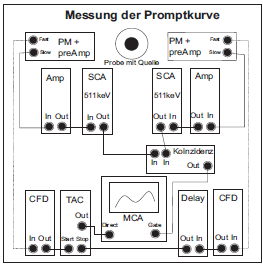
\includegraphics{graphics/setup_time}
}
  \caption{Set up for measuring the prompt curve and the time calibration.}
  \label{fig:setup_time}
\end{figure}
We set the delay between one CFD and the TAC to $\unit[12]{ns}$ and record the prompt curve displayed in figure \ref{fig:ana_prompt}.
\begin{figure}[H]
  \resizebox{0.8\textwidth}{!}{
    \begin{tikzpicture}[gnuplot]
%% generated with GNUPLOT 4.4p0 (Lua 5.1.4; terminal rev. 97, script rev. 96a)
%% 17.04.2010 13:45:42
\gpcolor{gp lt color border}
\gpsetlinetype{gp lt border}
\gpsetlinewidth{1.00}
\draw[gp path] (1.688,0.985)--(1.868,0.985);
\draw[gp path] (12.039,0.985)--(11.859,0.985);
\node[gp node right] at (1.504,0.985) { 0};
\draw[gp path] (1.688,2.042)--(1.868,2.042);
\draw[gp path] (12.039,2.042)--(11.859,2.042);
\node[gp node right] at (1.504,2.042) { 100};
\draw[gp path] (1.688,3.098)--(1.868,3.098);
\draw[gp path] (12.039,3.098)--(11.859,3.098);
\node[gp node right] at (1.504,3.098) { 200};
\draw[gp path] (1.688,4.155)--(1.868,4.155);
\draw[gp path] (12.039,4.155)--(11.859,4.155);
\node[gp node right] at (1.504,4.155) { 300};
\draw[gp path] (1.688,5.211)--(1.868,5.211);
\draw[gp path] (12.039,5.211)--(11.859,5.211);
\node[gp node right] at (1.504,5.211) { 400};
\draw[gp path] (1.688,6.268)--(1.868,6.268);
\draw[gp path] (12.039,6.268)--(11.859,6.268);
\node[gp node right] at (1.504,6.268) { 500};
\draw[gp path] (1.688,7.324)--(1.868,7.324);
\draw[gp path] (12.039,7.324)--(11.859,7.324);
\node[gp node right] at (1.504,7.324) { 600};
\draw[gp path] (1.688,8.381)--(1.868,8.381);
\draw[gp path] (12.039,8.381)--(11.859,8.381);
\node[gp node right] at (1.504,8.381) { 700};
\draw[gp path] (2.263,0.985)--(2.263,1.165);
\draw[gp path] (2.263,8.381)--(2.263,8.201);
\node[gp node center] at (2.263,0.677) { 1800};
\draw[gp path] (3.413,0.985)--(3.413,1.165);
\draw[gp path] (3.413,8.381)--(3.413,8.201);
\node[gp node center] at (3.413,0.677) { 2000};
\draw[gp path] (4.563,0.985)--(4.563,1.165);
\draw[gp path] (4.563,8.381)--(4.563,8.201);
\node[gp node center] at (4.563,0.677) { 2200};
\draw[gp path] (5.713,0.985)--(5.713,1.165);
\draw[gp path] (5.713,8.381)--(5.713,8.201);
\node[gp node center] at (5.713,0.677) { 2400};
\draw[gp path] (6.864,0.985)--(6.864,1.165);
\draw[gp path] (6.864,8.381)--(6.864,8.201);
\node[gp node center] at (6.864,0.677) { 2600};
\draw[gp path] (8.014,0.985)--(8.014,1.165);
\draw[gp path] (8.014,8.381)--(8.014,8.201);
\node[gp node center] at (8.014,0.677) { 2800};
\draw[gp path] (9.164,0.985)--(9.164,1.165);
\draw[gp path] (9.164,8.381)--(9.164,8.201);
\node[gp node center] at (9.164,0.677) { 3000};
\draw[gp path] (10.314,0.985)--(10.314,1.165);
\draw[gp path] (10.314,8.381)--(10.314,8.201);
\node[gp node center] at (10.314,0.677) { 3200};
\draw[gp path] (11.464,0.985)--(11.464,1.165);
\draw[gp path] (11.464,8.381)--(11.464,8.201);
\node[gp node center] at (11.464,0.677) { 3400};
\draw[gp path] (1.688,8.381)--(1.688,0.985)--(12.039,0.985)--(12.039,8.381)--cycle;
\node[gp node center,rotate=-270] at (0.430,4.683) {Count};
\node[gp node center] at (6.863,0.215) {Channel};
\node[gp node right] at (10.571,8.047) {Measured Data};
\gpcolor{gp lt color 0}
\gpsetpointsize{1.20}
\gppoint{gp mark 7}{(1.688,0.985)}
\gppoint{gp mark 7}{(1.694,0.985)}
\gppoint{gp mark 7}{(1.700,0.996)}
\gppoint{gp mark 7}{(1.705,0.985)}
\gppoint{gp mark 7}{(1.711,0.985)}
\gppoint{gp mark 7}{(1.717,0.985)}
\gppoint{gp mark 7}{(1.723,0.985)}
\gppoint{gp mark 7}{(1.728,0.996)}
\gppoint{gp mark 7}{(1.734,0.985)}
\gppoint{gp mark 7}{(1.740,0.996)}
\gppoint{gp mark 7}{(1.746,0.985)}
\gppoint{gp mark 7}{(1.751,0.985)}
\gppoint{gp mark 7}{(1.757,0.985)}
\gppoint{gp mark 7}{(1.763,0.985)}
\gppoint{gp mark 7}{(1.769,0.996)}
\gppoint{gp mark 7}{(1.774,0.985)}
\gppoint{gp mark 7}{(1.780,0.985)}
\gppoint{gp mark 7}{(1.786,0.985)}
\gppoint{gp mark 7}{(1.792,0.985)}
\gppoint{gp mark 7}{(1.797,0.985)}
\gppoint{gp mark 7}{(1.803,1.006)}
\gppoint{gp mark 7}{(1.809,0.985)}
\gppoint{gp mark 7}{(1.815,0.996)}
\gppoint{gp mark 7}{(1.820,0.985)}
\gppoint{gp mark 7}{(1.826,0.985)}
\gppoint{gp mark 7}{(1.832,0.985)}
\gppoint{gp mark 7}{(1.838,0.985)}
\gppoint{gp mark 7}{(1.843,0.985)}
\gppoint{gp mark 7}{(1.849,0.985)}
\gppoint{gp mark 7}{(1.855,0.985)}
\gppoint{gp mark 7}{(1.861,0.985)}
\gppoint{gp mark 7}{(1.866,0.985)}
\gppoint{gp mark 7}{(1.872,0.985)}
\gppoint{gp mark 7}{(1.878,1.006)}
\gppoint{gp mark 7}{(1.884,0.985)}
\gppoint{gp mark 7}{(1.889,0.985)}
\gppoint{gp mark 7}{(1.895,0.985)}
\gppoint{gp mark 7}{(1.901,0.985)}
\gppoint{gp mark 7}{(1.907,0.985)}
\gppoint{gp mark 7}{(1.912,0.996)}
\gppoint{gp mark 7}{(1.918,0.985)}
\gppoint{gp mark 7}{(1.924,0.985)}
\gppoint{gp mark 7}{(1.930,0.985)}
\gppoint{gp mark 7}{(1.935,0.985)}
\gppoint{gp mark 7}{(1.941,0.996)}
\gppoint{gp mark 7}{(1.947,0.985)}
\gppoint{gp mark 7}{(1.953,0.985)}
\gppoint{gp mark 7}{(1.958,0.985)}
\gppoint{gp mark 7}{(1.964,0.985)}
\gppoint{gp mark 7}{(1.970,0.985)}
\gppoint{gp mark 7}{(1.976,0.985)}
\gppoint{gp mark 7}{(1.981,0.985)}
\gppoint{gp mark 7}{(1.987,0.985)}
\gppoint{gp mark 7}{(1.993,0.985)}
\gppoint{gp mark 7}{(1.999,0.985)}
\gppoint{gp mark 7}{(2.004,0.985)}
\gppoint{gp mark 7}{(2.010,0.985)}
\gppoint{gp mark 7}{(2.016,0.985)}
\gppoint{gp mark 7}{(2.022,0.985)}
\gppoint{gp mark 7}{(2.027,0.985)}
\gppoint{gp mark 7}{(2.033,0.985)}
\gppoint{gp mark 7}{(2.039,0.985)}
\gppoint{gp mark 7}{(2.045,0.985)}
\gppoint{gp mark 7}{(2.050,0.985)}
\gppoint{gp mark 7}{(2.056,0.985)}
\gppoint{gp mark 7}{(2.062,0.985)}
\gppoint{gp mark 7}{(2.068,0.985)}
\gppoint{gp mark 7}{(2.073,0.985)}
\gppoint{gp mark 7}{(2.079,0.985)}
\gppoint{gp mark 7}{(2.085,0.985)}
\gppoint{gp mark 7}{(2.091,0.985)}
\gppoint{gp mark 7}{(2.096,0.985)}
\gppoint{gp mark 7}{(2.102,1.006)}
\gppoint{gp mark 7}{(2.108,0.985)}
\gppoint{gp mark 7}{(2.114,0.985)}
\gppoint{gp mark 7}{(2.119,0.996)}
\gppoint{gp mark 7}{(2.125,0.985)}
\gppoint{gp mark 7}{(2.131,0.985)}
\gppoint{gp mark 7}{(2.137,0.985)}
\gppoint{gp mark 7}{(2.142,0.985)}
\gppoint{gp mark 7}{(2.148,0.996)}
\gppoint{gp mark 7}{(2.154,0.985)}
\gppoint{gp mark 7}{(2.160,0.985)}
\gppoint{gp mark 7}{(2.165,0.985)}
\gppoint{gp mark 7}{(2.171,0.996)}
\gppoint{gp mark 7}{(2.177,0.996)}
\gppoint{gp mark 7}{(2.183,0.985)}
\gppoint{gp mark 7}{(2.188,0.985)}
\gppoint{gp mark 7}{(2.194,0.985)}
\gppoint{gp mark 7}{(2.200,0.985)}
\gppoint{gp mark 7}{(2.206,0.985)}
\gppoint{gp mark 7}{(2.211,0.996)}
\gppoint{gp mark 7}{(2.217,0.985)}
\gppoint{gp mark 7}{(2.223,0.985)}
\gppoint{gp mark 7}{(2.229,0.985)}
\gppoint{gp mark 7}{(2.234,0.985)}
\gppoint{gp mark 7}{(2.240,0.985)}
\gppoint{gp mark 7}{(2.246,0.985)}
\gppoint{gp mark 7}{(2.252,0.996)}
\gppoint{gp mark 7}{(2.257,0.985)}
\gppoint{gp mark 7}{(2.263,0.985)}
\gppoint{gp mark 7}{(2.269,0.985)}
\gppoint{gp mark 7}{(2.275,0.985)}
\gppoint{gp mark 7}{(2.280,0.985)}
\gppoint{gp mark 7}{(2.286,0.985)}
\gppoint{gp mark 7}{(2.292,0.996)}
\gppoint{gp mark 7}{(2.298,0.985)}
\gppoint{gp mark 7}{(2.303,0.996)}
\gppoint{gp mark 7}{(2.309,0.996)}
\gppoint{gp mark 7}{(2.315,0.985)}
\gppoint{gp mark 7}{(2.321,0.996)}
\gppoint{gp mark 7}{(2.326,0.985)}
\gppoint{gp mark 7}{(2.332,0.985)}
\gppoint{gp mark 7}{(2.338,0.996)}
\gppoint{gp mark 7}{(2.344,0.996)}
\gppoint{gp mark 7}{(2.349,0.985)}
\gppoint{gp mark 7}{(2.355,0.985)}
\gppoint{gp mark 7}{(2.361,0.985)}
\gppoint{gp mark 7}{(2.367,0.985)}
\gppoint{gp mark 7}{(2.372,0.985)}
\gppoint{gp mark 7}{(2.378,0.996)}
\gppoint{gp mark 7}{(2.384,0.985)}
\gppoint{gp mark 7}{(2.390,0.985)}
\gppoint{gp mark 7}{(2.395,0.996)}
\gppoint{gp mark 7}{(2.401,0.996)}
\gppoint{gp mark 7}{(2.407,0.985)}
\gppoint{gp mark 7}{(2.413,0.985)}
\gppoint{gp mark 7}{(2.418,0.996)}
\gppoint{gp mark 7}{(2.424,0.985)}
\gppoint{gp mark 7}{(2.430,0.985)}
\gppoint{gp mark 7}{(2.436,0.985)}
\gppoint{gp mark 7}{(2.441,1.006)}
\gppoint{gp mark 7}{(2.447,0.985)}
\gppoint{gp mark 7}{(2.453,0.985)}
\gppoint{gp mark 7}{(2.459,0.985)}
\gppoint{gp mark 7}{(2.464,0.985)}
\gppoint{gp mark 7}{(2.470,0.985)}
\gppoint{gp mark 7}{(2.476,0.996)}
\gppoint{gp mark 7}{(2.482,0.985)}
\gppoint{gp mark 7}{(2.487,0.985)}
\gppoint{gp mark 7}{(2.493,0.985)}
\gppoint{gp mark 7}{(2.499,0.985)}
\gppoint{gp mark 7}{(2.505,0.996)}
\gppoint{gp mark 7}{(2.510,0.985)}
\gppoint{gp mark 7}{(2.516,0.985)}
\gppoint{gp mark 7}{(2.522,0.985)}
\gppoint{gp mark 7}{(2.528,0.985)}
\gppoint{gp mark 7}{(2.533,0.996)}
\gppoint{gp mark 7}{(2.539,0.996)}
\gppoint{gp mark 7}{(2.545,0.985)}
\gppoint{gp mark 7}{(2.551,0.996)}
\gppoint{gp mark 7}{(2.556,1.006)}
\gppoint{gp mark 7}{(2.562,0.985)}
\gppoint{gp mark 7}{(2.568,0.996)}
\gppoint{gp mark 7}{(2.574,0.985)}
\gppoint{gp mark 7}{(2.579,0.985)}
\gppoint{gp mark 7}{(2.585,0.985)}
\gppoint{gp mark 7}{(2.591,0.996)}
\gppoint{gp mark 7}{(2.597,1.006)}
\gppoint{gp mark 7}{(2.602,0.996)}
\gppoint{gp mark 7}{(2.608,0.985)}
\gppoint{gp mark 7}{(2.614,0.985)}
\gppoint{gp mark 7}{(2.620,1.006)}
\gppoint{gp mark 7}{(2.625,0.985)}
\gppoint{gp mark 7}{(2.631,0.996)}
\gppoint{gp mark 7}{(2.637,0.996)}
\gppoint{gp mark 7}{(2.643,0.985)}
\gppoint{gp mark 7}{(2.648,0.985)}
\gppoint{gp mark 7}{(2.654,0.985)}
\gppoint{gp mark 7}{(2.660,0.985)}
\gppoint{gp mark 7}{(2.666,0.985)}
\gppoint{gp mark 7}{(2.671,0.985)}
\gppoint{gp mark 7}{(2.677,0.985)}
\gppoint{gp mark 7}{(2.683,0.985)}
\gppoint{gp mark 7}{(2.689,0.996)}
\gppoint{gp mark 7}{(2.694,0.996)}
\gppoint{gp mark 7}{(2.700,0.985)}
\gppoint{gp mark 7}{(2.706,0.985)}
\gppoint{gp mark 7}{(2.712,0.996)}
\gppoint{gp mark 7}{(2.717,0.985)}
\gppoint{gp mark 7}{(2.723,0.985)}
\gppoint{gp mark 7}{(2.729,0.996)}
\gppoint{gp mark 7}{(2.735,0.985)}
\gppoint{gp mark 7}{(2.740,0.996)}
\gppoint{gp mark 7}{(2.746,0.985)}
\gppoint{gp mark 7}{(2.752,0.996)}
\gppoint{gp mark 7}{(2.758,0.996)}
\gppoint{gp mark 7}{(2.763,0.985)}
\gppoint{gp mark 7}{(2.769,0.985)}
\gppoint{gp mark 7}{(2.775,0.985)}
\gppoint{gp mark 7}{(2.781,0.985)}
\gppoint{gp mark 7}{(2.786,0.985)}
\gppoint{gp mark 7}{(2.792,0.985)}
\gppoint{gp mark 7}{(2.798,0.985)}
\gppoint{gp mark 7}{(2.804,0.985)}
\gppoint{gp mark 7}{(2.809,0.985)}
\gppoint{gp mark 7}{(2.815,0.985)}
\gppoint{gp mark 7}{(2.821,0.996)}
\gppoint{gp mark 7}{(2.827,0.985)}
\gppoint{gp mark 7}{(2.832,0.985)}
\gppoint{gp mark 7}{(2.838,0.996)}
\gppoint{gp mark 7}{(2.844,0.985)}
\gppoint{gp mark 7}{(2.850,0.985)}
\gppoint{gp mark 7}{(2.855,0.985)}
\gppoint{gp mark 7}{(2.861,0.985)}
\gppoint{gp mark 7}{(2.867,1.006)}
\gppoint{gp mark 7}{(2.873,0.996)}
\gppoint{gp mark 7}{(2.878,1.006)}
\gppoint{gp mark 7}{(2.884,0.996)}
\gppoint{gp mark 7}{(2.890,0.985)}
\gppoint{gp mark 7}{(2.896,0.985)}
\gppoint{gp mark 7}{(2.901,0.985)}
\gppoint{gp mark 7}{(2.907,0.985)}
\gppoint{gp mark 7}{(2.913,0.985)}
\gppoint{gp mark 7}{(2.919,0.985)}
\gppoint{gp mark 7}{(2.924,1.006)}
\gppoint{gp mark 7}{(2.930,0.996)}
\gppoint{gp mark 7}{(2.936,1.006)}
\gppoint{gp mark 7}{(2.942,0.985)}
\gppoint{gp mark 7}{(2.947,0.996)}
\gppoint{gp mark 7}{(2.953,0.996)}
\gppoint{gp mark 7}{(2.959,0.985)}
\gppoint{gp mark 7}{(2.965,0.985)}
\gppoint{gp mark 7}{(2.970,0.985)}
\gppoint{gp mark 7}{(2.976,0.985)}
\gppoint{gp mark 7}{(2.982,0.996)}
\gppoint{gp mark 7}{(2.988,0.996)}
\gppoint{gp mark 7}{(2.993,0.985)}
\gppoint{gp mark 7}{(2.999,0.985)}
\gppoint{gp mark 7}{(3.005,1.006)}
\gppoint{gp mark 7}{(3.011,0.985)}
\gppoint{gp mark 7}{(3.016,0.985)}
\gppoint{gp mark 7}{(3.022,0.985)}
\gppoint{gp mark 7}{(3.028,0.985)}
\gppoint{gp mark 7}{(3.034,1.006)}
\gppoint{gp mark 7}{(3.039,0.985)}
\gppoint{gp mark 7}{(3.045,0.985)}
\gppoint{gp mark 7}{(3.051,1.006)}
\gppoint{gp mark 7}{(3.057,0.985)}
\gppoint{gp mark 7}{(3.062,0.985)}
\gppoint{gp mark 7}{(3.068,0.985)}
\gppoint{gp mark 7}{(3.074,0.985)}
\gppoint{gp mark 7}{(3.080,0.985)}
\gppoint{gp mark 7}{(3.085,0.985)}
\gppoint{gp mark 7}{(3.091,1.006)}
\gppoint{gp mark 7}{(3.097,0.985)}
\gppoint{gp mark 7}{(3.103,0.985)}
\gppoint{gp mark 7}{(3.108,0.985)}
\gppoint{gp mark 7}{(3.114,0.996)}
\gppoint{gp mark 7}{(3.120,0.985)}
\gppoint{gp mark 7}{(3.126,0.985)}
\gppoint{gp mark 7}{(3.131,0.985)}
\gppoint{gp mark 7}{(3.137,0.985)}
\gppoint{gp mark 7}{(3.143,0.996)}
\gppoint{gp mark 7}{(3.149,0.985)}
\gppoint{gp mark 7}{(3.154,0.985)}
\gppoint{gp mark 7}{(3.160,0.996)}
\gppoint{gp mark 7}{(3.166,1.017)}
\gppoint{gp mark 7}{(3.172,1.006)}
\gppoint{gp mark 7}{(3.177,0.985)}
\gppoint{gp mark 7}{(3.183,0.985)}
\gppoint{gp mark 7}{(3.189,0.985)}
\gppoint{gp mark 7}{(3.195,0.985)}
\gppoint{gp mark 7}{(3.200,0.996)}
\gppoint{gp mark 7}{(3.206,0.996)}
\gppoint{gp mark 7}{(3.212,0.996)}
\gppoint{gp mark 7}{(3.218,0.996)}
\gppoint{gp mark 7}{(3.223,0.996)}
\gppoint{gp mark 7}{(3.229,0.996)}
\gppoint{gp mark 7}{(3.235,0.985)}
\gppoint{gp mark 7}{(3.241,0.985)}
\gppoint{gp mark 7}{(3.246,0.985)}
\gppoint{gp mark 7}{(3.252,0.985)}
\gppoint{gp mark 7}{(3.258,0.985)}
\gppoint{gp mark 7}{(3.264,0.985)}
\gppoint{gp mark 7}{(3.269,0.985)}
\gppoint{gp mark 7}{(3.275,0.996)}
\gppoint{gp mark 7}{(3.281,1.006)}
\gppoint{gp mark 7}{(3.287,0.985)}
\gppoint{gp mark 7}{(3.292,0.985)}
\gppoint{gp mark 7}{(3.298,0.996)}
\gppoint{gp mark 7}{(3.304,0.985)}
\gppoint{gp mark 7}{(3.310,0.985)}
\gppoint{gp mark 7}{(3.315,0.985)}
\gppoint{gp mark 7}{(3.321,0.996)}
\gppoint{gp mark 7}{(3.327,0.985)}
\gppoint{gp mark 7}{(3.333,0.996)}
\gppoint{gp mark 7}{(3.338,0.985)}
\gppoint{gp mark 7}{(3.344,0.985)}
\gppoint{gp mark 7}{(3.350,1.006)}
\gppoint{gp mark 7}{(3.356,0.985)}
\gppoint{gp mark 7}{(3.361,0.985)}
\gppoint{gp mark 7}{(3.367,0.985)}
\gppoint{gp mark 7}{(3.373,0.985)}
\gppoint{gp mark 7}{(3.379,1.006)}
\gppoint{gp mark 7}{(3.384,0.985)}
\gppoint{gp mark 7}{(3.390,0.985)}
\gppoint{gp mark 7}{(3.396,1.006)}
\gppoint{gp mark 7}{(3.402,0.985)}
\gppoint{gp mark 7}{(3.407,0.985)}
\gppoint{gp mark 7}{(3.413,0.996)}
\gppoint{gp mark 7}{(3.419,0.985)}
\gppoint{gp mark 7}{(3.425,0.996)}
\gppoint{gp mark 7}{(3.430,0.996)}
\gppoint{gp mark 7}{(3.436,0.996)}
\gppoint{gp mark 7}{(3.442,1.006)}
\gppoint{gp mark 7}{(3.448,0.996)}
\gppoint{gp mark 7}{(3.453,0.996)}
\gppoint{gp mark 7}{(3.459,0.996)}
\gppoint{gp mark 7}{(3.465,0.985)}
\gppoint{gp mark 7}{(3.471,0.985)}
\gppoint{gp mark 7}{(3.476,0.996)}
\gppoint{gp mark 7}{(3.482,0.996)}
\gppoint{gp mark 7}{(3.488,0.985)}
\gppoint{gp mark 7}{(3.494,0.985)}
\gppoint{gp mark 7}{(3.499,0.985)}
\gppoint{gp mark 7}{(3.505,0.996)}
\gppoint{gp mark 7}{(3.511,0.985)}
\gppoint{gp mark 7}{(3.517,0.985)}
\gppoint{gp mark 7}{(3.522,0.985)}
\gppoint{gp mark 7}{(3.528,0.996)}
\gppoint{gp mark 7}{(3.534,0.996)}
\gppoint{gp mark 7}{(3.540,0.985)}
\gppoint{gp mark 7}{(3.545,0.985)}
\gppoint{gp mark 7}{(3.551,0.985)}
\gppoint{gp mark 7}{(3.557,1.006)}
\gppoint{gp mark 7}{(3.563,0.985)}
\gppoint{gp mark 7}{(3.568,0.996)}
\gppoint{gp mark 7}{(3.574,0.996)}
\gppoint{gp mark 7}{(3.580,0.985)}
\gppoint{gp mark 7}{(3.586,0.996)}
\gppoint{gp mark 7}{(3.591,0.985)}
\gppoint{gp mark 7}{(3.597,0.985)}
\gppoint{gp mark 7}{(3.603,1.017)}
\gppoint{gp mark 7}{(3.609,0.996)}
\gppoint{gp mark 7}{(3.614,0.996)}
\gppoint{gp mark 7}{(3.620,0.996)}
\gppoint{gp mark 7}{(3.626,0.985)}
\gppoint{gp mark 7}{(3.632,0.996)}
\gppoint{gp mark 7}{(3.637,0.996)}
\gppoint{gp mark 7}{(3.643,0.996)}
\gppoint{gp mark 7}{(3.649,0.985)}
\gppoint{gp mark 7}{(3.655,0.985)}
\gppoint{gp mark 7}{(3.660,1.006)}
\gppoint{gp mark 7}{(3.666,1.006)}
\gppoint{gp mark 7}{(3.672,0.985)}
\gppoint{gp mark 7}{(3.678,1.006)}
\gppoint{gp mark 7}{(3.683,0.985)}
\gppoint{gp mark 7}{(3.689,0.996)}
\gppoint{gp mark 7}{(3.695,0.985)}
\gppoint{gp mark 7}{(3.701,0.996)}
\gppoint{gp mark 7}{(3.706,1.017)}
\gppoint{gp mark 7}{(3.712,0.985)}
\gppoint{gp mark 7}{(3.718,0.985)}
\gppoint{gp mark 7}{(3.724,0.985)}
\gppoint{gp mark 7}{(3.729,0.985)}
\gppoint{gp mark 7}{(3.735,0.996)}
\gppoint{gp mark 7}{(3.741,0.996)}
\gppoint{gp mark 7}{(3.747,0.985)}
\gppoint{gp mark 7}{(3.752,0.985)}
\gppoint{gp mark 7}{(3.758,0.996)}
\gppoint{gp mark 7}{(3.764,1.006)}
\gppoint{gp mark 7}{(3.770,0.985)}
\gppoint{gp mark 7}{(3.775,1.006)}
\gppoint{gp mark 7}{(3.781,0.985)}
\gppoint{gp mark 7}{(3.787,0.985)}
\gppoint{gp mark 7}{(3.793,0.985)}
\gppoint{gp mark 7}{(3.798,1.006)}
\gppoint{gp mark 7}{(3.804,0.996)}
\gppoint{gp mark 7}{(3.810,0.996)}
\gppoint{gp mark 7}{(3.816,0.985)}
\gppoint{gp mark 7}{(3.821,0.985)}
\gppoint{gp mark 7}{(3.827,0.996)}
\gppoint{gp mark 7}{(3.833,0.985)}
\gppoint{gp mark 7}{(3.839,0.985)}
\gppoint{gp mark 7}{(3.844,0.985)}
\gppoint{gp mark 7}{(3.850,0.996)}
\gppoint{gp mark 7}{(3.856,0.996)}
\gppoint{gp mark 7}{(3.862,0.985)}
\gppoint{gp mark 7}{(3.867,0.985)}
\gppoint{gp mark 7}{(3.873,0.985)}
\gppoint{gp mark 7}{(3.879,0.996)}
\gppoint{gp mark 7}{(3.885,0.985)}
\gppoint{gp mark 7}{(3.890,0.985)}
\gppoint{gp mark 7}{(3.896,1.006)}
\gppoint{gp mark 7}{(3.902,0.996)}
\gppoint{gp mark 7}{(3.908,0.996)}
\gppoint{gp mark 7}{(3.913,1.006)}
\gppoint{gp mark 7}{(3.919,0.996)}
\gppoint{gp mark 7}{(3.925,0.985)}
\gppoint{gp mark 7}{(3.931,1.006)}
\gppoint{gp mark 7}{(3.936,0.996)}
\gppoint{gp mark 7}{(3.942,0.996)}
\gppoint{gp mark 7}{(3.948,1.006)}
\gppoint{gp mark 7}{(3.954,0.996)}
\gppoint{gp mark 7}{(3.959,0.985)}
\gppoint{gp mark 7}{(3.965,1.006)}
\gppoint{gp mark 7}{(3.971,0.996)}
\gppoint{gp mark 7}{(3.977,0.985)}
\gppoint{gp mark 7}{(3.982,0.985)}
\gppoint{gp mark 7}{(3.988,0.996)}
\gppoint{gp mark 7}{(3.994,0.996)}
\gppoint{gp mark 7}{(4.000,0.985)}
\gppoint{gp mark 7}{(4.005,0.985)}
\gppoint{gp mark 7}{(4.011,0.985)}
\gppoint{gp mark 7}{(4.017,0.985)}
\gppoint{gp mark 7}{(4.023,0.996)}
\gppoint{gp mark 7}{(4.028,0.985)}
\gppoint{gp mark 7}{(4.034,0.996)}
\gppoint{gp mark 7}{(4.040,0.996)}
\gppoint{gp mark 7}{(4.046,0.996)}
\gppoint{gp mark 7}{(4.051,0.996)}
\gppoint{gp mark 7}{(4.057,0.996)}
\gppoint{gp mark 7}{(4.063,0.985)}
\gppoint{gp mark 7}{(4.069,1.006)}
\gppoint{gp mark 7}{(4.074,1.006)}
\gppoint{gp mark 7}{(4.080,0.996)}
\gppoint{gp mark 7}{(4.086,0.985)}
\gppoint{gp mark 7}{(4.092,0.996)}
\gppoint{gp mark 7}{(4.097,0.996)}
\gppoint{gp mark 7}{(4.103,0.985)}
\gppoint{gp mark 7}{(4.109,1.017)}
\gppoint{gp mark 7}{(4.115,0.985)}
\gppoint{gp mark 7}{(4.120,1.006)}
\gppoint{gp mark 7}{(4.126,0.996)}
\gppoint{gp mark 7}{(4.132,0.996)}
\gppoint{gp mark 7}{(4.138,1.006)}
\gppoint{gp mark 7}{(4.143,1.006)}
\gppoint{gp mark 7}{(4.149,0.996)}
\gppoint{gp mark 7}{(4.155,1.017)}
\gppoint{gp mark 7}{(4.161,0.985)}
\gppoint{gp mark 7}{(4.166,0.985)}
\gppoint{gp mark 7}{(4.172,0.985)}
\gppoint{gp mark 7}{(4.178,1.017)}
\gppoint{gp mark 7}{(4.184,1.017)}
\gppoint{gp mark 7}{(4.189,1.006)}
\gppoint{gp mark 7}{(4.195,0.996)}
\gppoint{gp mark 7}{(4.201,0.996)}
\gppoint{gp mark 7}{(4.207,0.996)}
\gppoint{gp mark 7}{(4.212,0.985)}
\gppoint{gp mark 7}{(4.218,0.985)}
\gppoint{gp mark 7}{(4.224,0.996)}
\gppoint{gp mark 7}{(4.230,0.985)}
\gppoint{gp mark 7}{(4.235,0.996)}
\gppoint{gp mark 7}{(4.241,1.006)}
\gppoint{gp mark 7}{(4.247,0.985)}
\gppoint{gp mark 7}{(4.253,0.996)}
\gppoint{gp mark 7}{(4.258,0.996)}
\gppoint{gp mark 7}{(4.264,0.996)}
\gppoint{gp mark 7}{(4.270,0.996)}
\gppoint{gp mark 7}{(4.276,0.996)}
\gppoint{gp mark 7}{(4.282,0.985)}
\gppoint{gp mark 7}{(4.287,0.996)}
\gppoint{gp mark 7}{(4.293,1.006)}
\gppoint{gp mark 7}{(4.299,0.985)}
\gppoint{gp mark 7}{(4.305,0.996)}
\gppoint{gp mark 7}{(4.310,0.996)}
\gppoint{gp mark 7}{(4.316,0.985)}
\gppoint{gp mark 7}{(4.322,0.985)}
\gppoint{gp mark 7}{(4.328,1.006)}
\gppoint{gp mark 7}{(4.333,1.006)}
\gppoint{gp mark 7}{(4.339,1.006)}
\gppoint{gp mark 7}{(4.345,1.006)}
\gppoint{gp mark 7}{(4.351,0.985)}
\gppoint{gp mark 7}{(4.356,1.006)}
\gppoint{gp mark 7}{(4.362,1.017)}
\gppoint{gp mark 7}{(4.368,0.996)}
\gppoint{gp mark 7}{(4.374,0.996)}
\gppoint{gp mark 7}{(4.379,0.985)}
\gppoint{gp mark 7}{(4.385,0.985)}
\gppoint{gp mark 7}{(4.391,1.006)}
\gppoint{gp mark 7}{(4.397,1.017)}
\gppoint{gp mark 7}{(4.402,0.985)}
\gppoint{gp mark 7}{(4.408,0.996)}
\gppoint{gp mark 7}{(4.414,1.006)}
\gppoint{gp mark 7}{(4.420,0.996)}
\gppoint{gp mark 7}{(4.425,0.996)}
\gppoint{gp mark 7}{(4.431,1.006)}
\gppoint{gp mark 7}{(4.437,0.996)}
\gppoint{gp mark 7}{(4.443,1.017)}
\gppoint{gp mark 7}{(4.448,0.996)}
\gppoint{gp mark 7}{(4.454,1.017)}
\gppoint{gp mark 7}{(4.460,0.996)}
\gppoint{gp mark 7}{(4.466,0.996)}
\gppoint{gp mark 7}{(4.471,0.996)}
\gppoint{gp mark 7}{(4.477,1.006)}
\gppoint{gp mark 7}{(4.483,0.996)}
\gppoint{gp mark 7}{(4.489,0.996)}
\gppoint{gp mark 7}{(4.494,1.017)}
\gppoint{gp mark 7}{(4.500,0.985)}
\gppoint{gp mark 7}{(4.506,1.027)}
\gppoint{gp mark 7}{(4.512,0.985)}
\gppoint{gp mark 7}{(4.517,1.017)}
\gppoint{gp mark 7}{(4.523,1.017)}
\gppoint{gp mark 7}{(4.529,0.985)}
\gppoint{gp mark 7}{(4.535,1.006)}
\gppoint{gp mark 7}{(4.540,0.996)}
\gppoint{gp mark 7}{(4.546,0.985)}
\gppoint{gp mark 7}{(4.552,0.996)}
\gppoint{gp mark 7}{(4.558,0.996)}
\gppoint{gp mark 7}{(4.563,0.985)}
\gppoint{gp mark 7}{(4.569,1.006)}
\gppoint{gp mark 7}{(4.575,1.017)}
\gppoint{gp mark 7}{(4.581,0.985)}
\gppoint{gp mark 7}{(4.586,0.985)}
\gppoint{gp mark 7}{(4.592,0.996)}
\gppoint{gp mark 7}{(4.598,1.017)}
\gppoint{gp mark 7}{(4.604,0.985)}
\gppoint{gp mark 7}{(4.609,1.006)}
\gppoint{gp mark 7}{(4.615,0.985)}
\gppoint{gp mark 7}{(4.621,0.985)}
\gppoint{gp mark 7}{(4.627,0.985)}
\gppoint{gp mark 7}{(4.632,0.996)}
\gppoint{gp mark 7}{(4.638,1.017)}
\gppoint{gp mark 7}{(4.644,0.996)}
\gppoint{gp mark 7}{(4.650,0.985)}
\gppoint{gp mark 7}{(4.655,1.027)}
\gppoint{gp mark 7}{(4.661,0.985)}
\gppoint{gp mark 7}{(4.667,1.006)}
\gppoint{gp mark 7}{(4.673,0.996)}
\gppoint{gp mark 7}{(4.678,0.996)}
\gppoint{gp mark 7}{(4.684,1.038)}
\gppoint{gp mark 7}{(4.690,0.996)}
\gppoint{gp mark 7}{(4.696,1.006)}
\gppoint{gp mark 7}{(4.701,1.027)}
\gppoint{gp mark 7}{(4.707,1.017)}
\gppoint{gp mark 7}{(4.713,0.996)}
\gppoint{gp mark 7}{(4.719,1.017)}
\gppoint{gp mark 7}{(4.724,1.006)}
\gppoint{gp mark 7}{(4.730,1.038)}
\gppoint{gp mark 7}{(4.736,1.006)}
\gppoint{gp mark 7}{(4.742,1.017)}
\gppoint{gp mark 7}{(4.747,0.985)}
\gppoint{gp mark 7}{(4.753,1.006)}
\gppoint{gp mark 7}{(4.759,0.996)}
\gppoint{gp mark 7}{(4.765,0.996)}
\gppoint{gp mark 7}{(4.770,1.006)}
\gppoint{gp mark 7}{(4.776,0.996)}
\gppoint{gp mark 7}{(4.782,1.006)}
\gppoint{gp mark 7}{(4.788,0.996)}
\gppoint{gp mark 7}{(4.793,0.996)}
\gppoint{gp mark 7}{(4.799,1.006)}
\gppoint{gp mark 7}{(4.805,0.985)}
\gppoint{gp mark 7}{(4.811,0.985)}
\gppoint{gp mark 7}{(4.816,0.985)}
\gppoint{gp mark 7}{(4.822,1.027)}
\gppoint{gp mark 7}{(4.828,1.017)}
\gppoint{gp mark 7}{(4.834,0.985)}
\gppoint{gp mark 7}{(4.839,0.996)}
\gppoint{gp mark 7}{(4.845,1.006)}
\gppoint{gp mark 7}{(4.851,1.017)}
\gppoint{gp mark 7}{(4.857,0.996)}
\gppoint{gp mark 7}{(4.862,0.996)}
\gppoint{gp mark 7}{(4.868,1.027)}
\gppoint{gp mark 7}{(4.874,0.985)}
\gppoint{gp mark 7}{(4.880,1.006)}
\gppoint{gp mark 7}{(4.885,1.006)}
\gppoint{gp mark 7}{(4.891,0.996)}
\gppoint{gp mark 7}{(4.897,1.006)}
\gppoint{gp mark 7}{(4.903,1.017)}
\gppoint{gp mark 7}{(4.908,0.985)}
\gppoint{gp mark 7}{(4.914,0.996)}
\gppoint{gp mark 7}{(4.920,1.038)}
\gppoint{gp mark 7}{(4.926,1.027)}
\gppoint{gp mark 7}{(4.931,1.017)}
\gppoint{gp mark 7}{(4.937,1.017)}
\gppoint{gp mark 7}{(4.943,0.985)}
\gppoint{gp mark 7}{(4.949,1.027)}
\gppoint{gp mark 7}{(4.954,1.006)}
\gppoint{gp mark 7}{(4.960,1.006)}
\gppoint{gp mark 7}{(4.966,1.027)}
\gppoint{gp mark 7}{(4.972,1.048)}
\gppoint{gp mark 7}{(4.977,1.006)}
\gppoint{gp mark 7}{(4.983,0.985)}
\gppoint{gp mark 7}{(4.989,0.985)}
\gppoint{gp mark 7}{(4.995,1.006)}
\gppoint{gp mark 7}{(5.000,1.017)}
\gppoint{gp mark 7}{(5.006,1.006)}
\gppoint{gp mark 7}{(5.012,0.985)}
\gppoint{gp mark 7}{(5.018,1.038)}
\gppoint{gp mark 7}{(5.023,1.006)}
\gppoint{gp mark 7}{(5.029,1.006)}
\gppoint{gp mark 7}{(5.035,1.006)}
\gppoint{gp mark 7}{(5.041,1.017)}
\gppoint{gp mark 7}{(5.046,1.017)}
\gppoint{gp mark 7}{(5.052,1.038)}
\gppoint{gp mark 7}{(5.058,1.017)}
\gppoint{gp mark 7}{(5.064,1.006)}
\gppoint{gp mark 7}{(5.069,1.017)}
\gppoint{gp mark 7}{(5.075,1.038)}
\gppoint{gp mark 7}{(5.081,0.996)}
\gppoint{gp mark 7}{(5.087,1.006)}
\gppoint{gp mark 7}{(5.092,1.006)}
\gppoint{gp mark 7}{(5.098,1.017)}
\gppoint{gp mark 7}{(5.104,1.017)}
\gppoint{gp mark 7}{(5.110,1.027)}
\gppoint{gp mark 7}{(5.115,0.996)}
\gppoint{gp mark 7}{(5.121,1.027)}
\gppoint{gp mark 7}{(5.127,1.006)}
\gppoint{gp mark 7}{(5.133,1.027)}
\gppoint{gp mark 7}{(5.138,1.006)}
\gppoint{gp mark 7}{(5.144,1.017)}
\gppoint{gp mark 7}{(5.150,0.996)}
\gppoint{gp mark 7}{(5.156,1.017)}
\gppoint{gp mark 7}{(5.161,1.027)}
\gppoint{gp mark 7}{(5.167,1.027)}
\gppoint{gp mark 7}{(5.173,1.027)}
\gppoint{gp mark 7}{(5.179,1.017)}
\gppoint{gp mark 7}{(5.184,1.027)}
\gppoint{gp mark 7}{(5.190,1.017)}
\gppoint{gp mark 7}{(5.196,1.027)}
\gppoint{gp mark 7}{(5.202,1.017)}
\gppoint{gp mark 7}{(5.207,1.006)}
\gppoint{gp mark 7}{(5.213,1.059)}
\gppoint{gp mark 7}{(5.219,1.006)}
\gppoint{gp mark 7}{(5.225,1.027)}
\gppoint{gp mark 7}{(5.230,1.017)}
\gppoint{gp mark 7}{(5.236,1.006)}
\gppoint{gp mark 7}{(5.242,1.006)}
\gppoint{gp mark 7}{(5.248,1.048)}
\gppoint{gp mark 7}{(5.253,0.996)}
\gppoint{gp mark 7}{(5.259,1.027)}
\gppoint{gp mark 7}{(5.265,1.038)}
\gppoint{gp mark 7}{(5.271,0.996)}
\gppoint{gp mark 7}{(5.276,0.996)}
\gppoint{gp mark 7}{(5.282,1.006)}
\gppoint{gp mark 7}{(5.288,1.017)}
\gppoint{gp mark 7}{(5.294,1.059)}
\gppoint{gp mark 7}{(5.299,1.059)}
\gppoint{gp mark 7}{(5.305,1.006)}
\gppoint{gp mark 7}{(5.311,1.059)}
\gppoint{gp mark 7}{(5.317,1.027)}
\gppoint{gp mark 7}{(5.322,1.059)}
\gppoint{gp mark 7}{(5.328,1.038)}
\gppoint{gp mark 7}{(5.334,1.027)}
\gppoint{gp mark 7}{(5.340,1.027)}
\gppoint{gp mark 7}{(5.345,1.048)}
\gppoint{gp mark 7}{(5.351,0.996)}
\gppoint{gp mark 7}{(5.357,1.027)}
\gppoint{gp mark 7}{(5.363,1.027)}
\gppoint{gp mark 7}{(5.368,1.038)}
\gppoint{gp mark 7}{(5.374,1.048)}
\gppoint{gp mark 7}{(5.380,1.027)}
\gppoint{gp mark 7}{(5.386,1.006)}
\gppoint{gp mark 7}{(5.391,1.070)}
\gppoint{gp mark 7}{(5.397,1.017)}
\gppoint{gp mark 7}{(5.403,1.059)}
\gppoint{gp mark 7}{(5.409,1.027)}
\gppoint{gp mark 7}{(5.414,1.017)}
\gppoint{gp mark 7}{(5.420,1.101)}
\gppoint{gp mark 7}{(5.426,1.048)}
\gppoint{gp mark 7}{(5.432,1.027)}
\gppoint{gp mark 7}{(5.437,1.027)}
\gppoint{gp mark 7}{(5.443,1.027)}
\gppoint{gp mark 7}{(5.449,1.027)}
\gppoint{gp mark 7}{(5.455,1.038)}
\gppoint{gp mark 7}{(5.460,1.027)}
\gppoint{gp mark 7}{(5.466,1.048)}
\gppoint{gp mark 7}{(5.472,1.006)}
\gppoint{gp mark 7}{(5.478,1.059)}
\gppoint{gp mark 7}{(5.483,1.027)}
\gppoint{gp mark 7}{(5.489,1.048)}
\gppoint{gp mark 7}{(5.495,1.048)}
\gppoint{gp mark 7}{(5.501,1.080)}
\gppoint{gp mark 7}{(5.506,1.070)}
\gppoint{gp mark 7}{(5.512,1.027)}
\gppoint{gp mark 7}{(5.518,1.038)}
\gppoint{gp mark 7}{(5.524,1.070)}
\gppoint{gp mark 7}{(5.529,1.048)}
\gppoint{gp mark 7}{(5.535,1.027)}
\gppoint{gp mark 7}{(5.541,1.006)}
\gppoint{gp mark 7}{(5.547,1.027)}
\gppoint{gp mark 7}{(5.552,1.048)}
\gppoint{gp mark 7}{(5.558,1.101)}
\gppoint{gp mark 7}{(5.564,1.027)}
\gppoint{gp mark 7}{(5.570,1.048)}
\gppoint{gp mark 7}{(5.575,1.101)}
\gppoint{gp mark 7}{(5.581,1.059)}
\gppoint{gp mark 7}{(5.587,1.006)}
\gppoint{gp mark 7}{(5.593,1.122)}
\gppoint{gp mark 7}{(5.598,1.091)}
\gppoint{gp mark 7}{(5.604,1.048)}
\gppoint{gp mark 7}{(5.610,1.027)}
\gppoint{gp mark 7}{(5.616,1.059)}
\gppoint{gp mark 7}{(5.621,1.080)}
\gppoint{gp mark 7}{(5.627,1.091)}
\gppoint{gp mark 7}{(5.633,1.091)}
\gppoint{gp mark 7}{(5.639,1.070)}
\gppoint{gp mark 7}{(5.644,1.059)}
\gppoint{gp mark 7}{(5.650,1.122)}
\gppoint{gp mark 7}{(5.656,1.101)}
\gppoint{gp mark 7}{(5.662,1.143)}
\gppoint{gp mark 7}{(5.667,1.080)}
\gppoint{gp mark 7}{(5.673,1.080)}
\gppoint{gp mark 7}{(5.679,1.070)}
\gppoint{gp mark 7}{(5.685,1.059)}
\gppoint{gp mark 7}{(5.690,1.154)}
\gppoint{gp mark 7}{(5.696,1.080)}
\gppoint{gp mark 7}{(5.702,1.143)}
\gppoint{gp mark 7}{(5.708,1.133)}
\gppoint{gp mark 7}{(5.713,1.175)}
\gppoint{gp mark 7}{(5.719,1.143)}
\gppoint{gp mark 7}{(5.725,1.070)}
\gppoint{gp mark 7}{(5.731,1.196)}
\gppoint{gp mark 7}{(5.736,1.165)}
\gppoint{gp mark 7}{(5.742,1.101)}
\gppoint{gp mark 7}{(5.748,1.091)}
\gppoint{gp mark 7}{(5.754,1.207)}
\gppoint{gp mark 7}{(5.759,1.101)}
\gppoint{gp mark 7}{(5.765,1.080)}
\gppoint{gp mark 7}{(5.771,1.080)}
\gppoint{gp mark 7}{(5.777,1.101)}
\gppoint{gp mark 7}{(5.782,1.143)}
\gppoint{gp mark 7}{(5.788,1.207)}
\gppoint{gp mark 7}{(5.794,1.133)}
\gppoint{gp mark 7}{(5.800,1.207)}
\gppoint{gp mark 7}{(5.805,1.154)}
\gppoint{gp mark 7}{(5.811,1.165)}
\gppoint{gp mark 7}{(5.817,1.112)}
\gppoint{gp mark 7}{(5.823,1.143)}
\gppoint{gp mark 7}{(5.828,1.228)}
\gppoint{gp mark 7}{(5.834,1.217)}
\gppoint{gp mark 7}{(5.840,1.228)}
\gppoint{gp mark 7}{(5.846,1.091)}
\gppoint{gp mark 7}{(5.851,1.217)}
\gppoint{gp mark 7}{(5.857,1.165)}
\gppoint{gp mark 7}{(5.863,1.239)}
\gppoint{gp mark 7}{(5.869,1.239)}
\gppoint{gp mark 7}{(5.874,1.334)}
\gppoint{gp mark 7}{(5.880,1.334)}
\gppoint{gp mark 7}{(5.886,1.228)}
\gppoint{gp mark 7}{(5.892,1.239)}
\gppoint{gp mark 7}{(5.897,1.291)}
\gppoint{gp mark 7}{(5.903,1.260)}
\gppoint{gp mark 7}{(5.909,1.281)}
\gppoint{gp mark 7}{(5.915,1.281)}
\gppoint{gp mark 7}{(5.920,1.270)}
\gppoint{gp mark 7}{(5.926,1.355)}
\gppoint{gp mark 7}{(5.932,1.270)}
\gppoint{gp mark 7}{(5.938,1.397)}
\gppoint{gp mark 7}{(5.943,1.313)}
\gppoint{gp mark 7}{(5.949,1.397)}
\gppoint{gp mark 7}{(5.955,1.281)}
\gppoint{gp mark 7}{(5.961,1.302)}
\gppoint{gp mark 7}{(5.966,1.429)}
\gppoint{gp mark 7}{(5.972,1.334)}
\gppoint{gp mark 7}{(5.978,1.482)}
\gppoint{gp mark 7}{(5.984,1.386)}
\gppoint{gp mark 7}{(5.989,1.344)}
\gppoint{gp mark 7}{(5.995,1.524)}
\gppoint{gp mark 7}{(6.001,1.376)}
\gppoint{gp mark 7}{(6.007,1.429)}
\gppoint{gp mark 7}{(6.012,1.471)}
\gppoint{gp mark 7}{(6.018,1.566)}
\gppoint{gp mark 7}{(6.024,1.418)}
\gppoint{gp mark 7}{(6.030,1.471)}
\gppoint{gp mark 7}{(6.035,1.608)}
\gppoint{gp mark 7}{(6.041,1.556)}
\gppoint{gp mark 7}{(6.047,1.566)}
\gppoint{gp mark 7}{(6.053,1.524)}
\gppoint{gp mark 7}{(6.058,1.545)}
\gppoint{gp mark 7}{(6.064,1.651)}
\gppoint{gp mark 7}{(6.070,1.534)}
\gppoint{gp mark 7}{(6.076,1.566)}
\gppoint{gp mark 7}{(6.081,1.672)}
\gppoint{gp mark 7}{(6.087,1.788)}
\gppoint{gp mark 7}{(6.093,1.693)}
\gppoint{gp mark 7}{(6.099,1.756)}
\gppoint{gp mark 7}{(6.104,1.756)}
\gppoint{gp mark 7}{(6.110,1.672)}
\gppoint{gp mark 7}{(6.116,1.661)}
\gppoint{gp mark 7}{(6.122,1.661)}
\gppoint{gp mark 7}{(6.127,1.915)}
\gppoint{gp mark 7}{(6.133,1.851)}
\gppoint{gp mark 7}{(6.139,1.788)}
\gppoint{gp mark 7}{(6.145,1.851)}
\gppoint{gp mark 7}{(6.150,1.820)}
\gppoint{gp mark 7}{(6.156,2.031)}
\gppoint{gp mark 7}{(6.162,2.010)}
\gppoint{gp mark 7}{(6.168,2.094)}
\gppoint{gp mark 7}{(6.173,1.978)}
\gppoint{gp mark 7}{(6.179,2.105)}
\gppoint{gp mark 7}{(6.185,2.042)}
\gppoint{gp mark 7}{(6.191,2.073)}
\gppoint{gp mark 7}{(6.196,2.063)}
\gppoint{gp mark 7}{(6.202,2.073)}
\gppoint{gp mark 7}{(6.208,2.137)}
\gppoint{gp mark 7}{(6.214,2.348)}
\gppoint{gp mark 7}{(6.219,2.285)}
\gppoint{gp mark 7}{(6.225,2.211)}
\gppoint{gp mark 7}{(6.231,2.094)}
\gppoint{gp mark 7}{(6.237,2.464)}
\gppoint{gp mark 7}{(6.242,2.380)}
\gppoint{gp mark 7}{(6.248,2.464)}
\gppoint{gp mark 7}{(6.254,2.337)}
\gppoint{gp mark 7}{(6.260,2.337)}
\gppoint{gp mark 7}{(6.265,2.464)}
\gppoint{gp mark 7}{(6.271,2.781)}
\gppoint{gp mark 7}{(6.277,2.644)}
\gppoint{gp mark 7}{(6.283,2.665)}
\gppoint{gp mark 7}{(6.288,2.950)}
\gppoint{gp mark 7}{(6.294,2.665)}
\gppoint{gp mark 7}{(6.300,2.654)}
\gppoint{gp mark 7}{(6.306,2.654)}
\gppoint{gp mark 7}{(6.311,2.992)}
\gppoint{gp mark 7}{(6.317,2.876)}
\gppoint{gp mark 7}{(6.323,2.823)}
\gppoint{gp mark 7}{(6.329,2.855)}
\gppoint{gp mark 7}{(6.334,2.813)}
\gppoint{gp mark 7}{(6.340,2.728)}
\gppoint{gp mark 7}{(6.346,3.119)}
\gppoint{gp mark 7}{(6.352,2.950)}
\gppoint{gp mark 7}{(6.357,3.214)}
\gppoint{gp mark 7}{(6.363,3.278)}
\gppoint{gp mark 7}{(6.369,3.479)}
\gppoint{gp mark 7}{(6.375,3.172)}
\gppoint{gp mark 7}{(6.380,3.119)}
\gppoint{gp mark 7}{(6.386,3.235)}
\gppoint{gp mark 7}{(6.392,3.299)}
\gppoint{gp mark 7}{(6.398,3.320)}
\gppoint{gp mark 7}{(6.403,3.563)}
\gppoint{gp mark 7}{(6.409,3.436)}
\gppoint{gp mark 7}{(6.415,3.542)}
\gppoint{gp mark 7}{(6.421,3.637)}
\gppoint{gp mark 7}{(6.426,3.626)}
\gppoint{gp mark 7}{(6.432,3.722)}
\gppoint{gp mark 7}{(6.438,3.743)}
\gppoint{gp mark 7}{(6.444,3.827)}
\gppoint{gp mark 7}{(6.449,4.081)}
\gppoint{gp mark 7}{(6.455,3.817)}
\gppoint{gp mark 7}{(6.461,3.933)}
\gppoint{gp mark 7}{(6.467,3.764)}
\gppoint{gp mark 7}{(6.472,4.060)}
\gppoint{gp mark 7}{(6.478,4.377)}
\gppoint{gp mark 7}{(6.484,4.208)}
\gppoint{gp mark 7}{(6.490,4.102)}
\gppoint{gp mark 7}{(6.495,4.408)}
\gppoint{gp mark 7}{(6.501,4.630)}
\gppoint{gp mark 7}{(6.507,4.271)}
\gppoint{gp mark 7}{(6.513,4.461)}
\gppoint{gp mark 7}{(6.518,4.440)}
\gppoint{gp mark 7}{(6.524,4.429)}
\gppoint{gp mark 7}{(6.530,4.525)}
\gppoint{gp mark 7}{(6.536,4.525)}
\gppoint{gp mark 7}{(6.541,4.905)}
\gppoint{gp mark 7}{(6.547,4.461)}
\gppoint{gp mark 7}{(6.553,4.704)}
\gppoint{gp mark 7}{(6.559,5.116)}
\gppoint{gp mark 7}{(6.564,5.243)}
\gppoint{gp mark 7}{(6.570,5.042)}
\gppoint{gp mark 7}{(6.576,4.915)}
\gppoint{gp mark 7}{(6.582,5.042)}
\gppoint{gp mark 7}{(6.587,5.180)}
\gppoint{gp mark 7}{(6.593,5.380)}
\gppoint{gp mark 7}{(6.599,5.000)}
\gppoint{gp mark 7}{(6.605,5.528)}
\gppoint{gp mark 7}{(6.610,5.972)}
\gppoint{gp mark 7}{(6.616,5.528)}
\gppoint{gp mark 7}{(6.622,5.169)}
\gppoint{gp mark 7}{(6.628,5.845)}
\gppoint{gp mark 7}{(6.633,5.835)}
\gppoint{gp mark 7}{(6.639,5.792)}
\gppoint{gp mark 7}{(6.645,5.993)}
\gppoint{gp mark 7}{(6.651,5.718)}
\gppoint{gp mark 7}{(6.656,6.109)}
\gppoint{gp mark 7}{(6.662,5.592)}
\gppoint{gp mark 7}{(6.668,5.644)}
\gppoint{gp mark 7}{(6.674,6.300)}
\gppoint{gp mark 7}{(6.679,5.835)}
\gppoint{gp mark 7}{(6.685,6.490)}
\gppoint{gp mark 7}{(6.691,6.532)}
\gppoint{gp mark 7}{(6.697,5.475)}
\gppoint{gp mark 7}{(6.702,6.278)}
\gppoint{gp mark 7}{(6.708,6.236)}
\gppoint{gp mark 7}{(6.714,6.300)}
\gppoint{gp mark 7}{(6.720,6.384)}
\gppoint{gp mark 7}{(6.725,5.814)}
\gppoint{gp mark 7}{(6.731,6.131)}
\gppoint{gp mark 7}{(6.737,6.247)}
\gppoint{gp mark 7}{(6.743,6.374)}
\gppoint{gp mark 7}{(6.748,6.363)}
\gppoint{gp mark 7}{(6.754,6.247)}
\gppoint{gp mark 7}{(6.760,6.574)}
\gppoint{gp mark 7}{(6.766,6.204)}
\gppoint{gp mark 7}{(6.771,6.701)}
\gppoint{gp mark 7}{(6.777,6.078)}
\gppoint{gp mark 7}{(6.783,6.912)}
\gppoint{gp mark 7}{(6.789,6.363)}
\gppoint{gp mark 7}{(6.794,6.194)}
\gppoint{gp mark 7}{(6.800,6.680)}
\gppoint{gp mark 7}{(6.806,6.564)}
\gppoint{gp mark 7}{(6.812,6.870)}
\gppoint{gp mark 7}{(6.817,6.923)}
\gppoint{gp mark 7}{(6.823,6.690)}
\gppoint{gp mark 7}{(6.829,6.426)}
\gppoint{gp mark 7}{(6.835,6.944)}
\gppoint{gp mark 7}{(6.840,6.627)}
\gppoint{gp mark 7}{(6.846,6.965)}
\gppoint{gp mark 7}{(6.852,6.912)}
\gppoint{gp mark 7}{(6.858,6.807)}
\gppoint{gp mark 7}{(6.864,7.187)}
\gppoint{gp mark 7}{(6.869,7.356)}
\gppoint{gp mark 7}{(6.875,7.103)}
\gppoint{gp mark 7}{(6.881,6.944)}
\gppoint{gp mark 7}{(6.887,6.912)}
\gppoint{gp mark 7}{(6.892,6.585)}
\gppoint{gp mark 7}{(6.898,7.356)}
\gppoint{gp mark 7}{(6.904,6.754)}
\gppoint{gp mark 7}{(6.910,6.617)}
\gppoint{gp mark 7}{(6.915,7.324)}
\gppoint{gp mark 7}{(6.921,7.282)}
\gppoint{gp mark 7}{(6.927,6.236)}
\gppoint{gp mark 7}{(6.933,6.997)}
\gppoint{gp mark 7}{(6.938,7.694)}
\gppoint{gp mark 7}{(6.944,6.923)}
\gppoint{gp mark 7}{(6.950,7.081)}
\gppoint{gp mark 7}{(6.956,7.388)}
\gppoint{gp mark 7}{(6.961,6.712)}
\gppoint{gp mark 7}{(6.967,6.564)}
\gppoint{gp mark 7}{(6.973,7.134)}
\gppoint{gp mark 7}{(6.979,6.860)}
\gppoint{gp mark 7}{(6.984,6.933)}
\gppoint{gp mark 7}{(6.990,7.071)}
\gppoint{gp mark 7}{(6.996,6.912)}
\gppoint{gp mark 7}{(7.002,6.902)}
\gppoint{gp mark 7}{(7.007,7.103)}
\gppoint{gp mark 7}{(7.013,6.617)}
\gppoint{gp mark 7}{(7.019,6.574)}
\gppoint{gp mark 7}{(7.025,6.817)}
\gppoint{gp mark 7}{(7.030,6.321)}
\gppoint{gp mark 7}{(7.036,6.986)}
\gppoint{gp mark 7}{(7.042,6.870)}
\gppoint{gp mark 7}{(7.048,7.145)}
\gppoint{gp mark 7}{(7.053,6.669)}
\gppoint{gp mark 7}{(7.059,6.733)}
\gppoint{gp mark 7}{(7.065,6.088)}
\gppoint{gp mark 7}{(7.071,6.574)}
\gppoint{gp mark 7}{(7.076,6.680)}
\gppoint{gp mark 7}{(7.082,6.754)}
\gppoint{gp mark 7}{(7.088,6.627)}
\gppoint{gp mark 7}{(7.094,6.310)}
\gppoint{gp mark 7}{(7.099,6.395)}
\gppoint{gp mark 7}{(7.105,6.374)}
\gppoint{gp mark 7}{(7.111,6.733)}
\gppoint{gp mark 7}{(7.117,6.300)}
\gppoint{gp mark 7}{(7.122,6.659)}
\gppoint{gp mark 7}{(7.128,5.961)}
\gppoint{gp mark 7}{(7.134,5.972)}
\gppoint{gp mark 7}{(7.140,6.638)}
\gppoint{gp mark 7}{(7.145,6.162)}
\gppoint{gp mark 7}{(7.151,6.374)}
\gppoint{gp mark 7}{(7.157,5.824)}
\gppoint{gp mark 7}{(7.163,6.416)}
\gppoint{gp mark 7}{(7.168,6.204)}
\gppoint{gp mark 7}{(7.174,6.204)}
\gppoint{gp mark 7}{(7.180,6.046)}
\gppoint{gp mark 7}{(7.186,6.046)}
\gppoint{gp mark 7}{(7.191,5.814)}
\gppoint{gp mark 7}{(7.197,6.215)}
\gppoint{gp mark 7}{(7.203,5.940)}
\gppoint{gp mark 7}{(7.209,5.940)}
\gppoint{gp mark 7}{(7.214,5.740)}
\gppoint{gp mark 7}{(7.220,6.078)}
\gppoint{gp mark 7}{(7.226,5.845)}
\gppoint{gp mark 7}{(7.232,5.856)}
\gppoint{gp mark 7}{(7.237,5.539)}
\gppoint{gp mark 7}{(7.243,5.571)}
\gppoint{gp mark 7}{(7.249,5.961)}
\gppoint{gp mark 7}{(7.255,5.919)}
\gppoint{gp mark 7}{(7.260,5.866)}
\gppoint{gp mark 7}{(7.266,5.602)}
\gppoint{gp mark 7}{(7.272,5.444)}
\gppoint{gp mark 7}{(7.278,5.602)}
\gppoint{gp mark 7}{(7.283,5.814)}
\gppoint{gp mark 7}{(7.289,5.655)}
\gppoint{gp mark 7}{(7.295,5.581)}
\gppoint{gp mark 7}{(7.301,5.095)}
\gppoint{gp mark 7}{(7.306,4.979)}
\gppoint{gp mark 7}{(7.312,5.074)}
\gppoint{gp mark 7}{(7.318,5.190)}
\gppoint{gp mark 7}{(7.324,4.947)}
\gppoint{gp mark 7}{(7.329,5.095)}
\gppoint{gp mark 7}{(7.335,5.401)}
\gppoint{gp mark 7}{(7.341,5.021)}
\gppoint{gp mark 7}{(7.347,4.894)}
\gppoint{gp mark 7}{(7.352,5.465)}
\gppoint{gp mark 7}{(7.358,4.683)}
\gppoint{gp mark 7}{(7.364,4.736)}
\gppoint{gp mark 7}{(7.370,4.757)}
\gppoint{gp mark 7}{(7.375,4.947)}
\gppoint{gp mark 7}{(7.381,4.757)}
\gppoint{gp mark 7}{(7.387,4.694)}
\gppoint{gp mark 7}{(7.393,4.461)}
\gppoint{gp mark 7}{(7.398,4.989)}
\gppoint{gp mark 7}{(7.404,4.588)}
\gppoint{gp mark 7}{(7.410,4.926)}
\gppoint{gp mark 7}{(7.416,4.873)}
\gppoint{gp mark 7}{(7.421,4.303)}
\gppoint{gp mark 7}{(7.427,4.271)}
\gppoint{gp mark 7}{(7.433,4.863)}
\gppoint{gp mark 7}{(7.439,4.081)}
\gppoint{gp mark 7}{(7.444,4.250)}
\gppoint{gp mark 7}{(7.450,4.683)}
\gppoint{gp mark 7}{(7.456,4.387)}
\gppoint{gp mark 7}{(7.462,4.123)}
\gppoint{gp mark 7}{(7.467,4.186)}
\gppoint{gp mark 7}{(7.473,4.313)}
\gppoint{gp mark 7}{(7.479,4.630)}
\gppoint{gp mark 7}{(7.485,4.155)}
\gppoint{gp mark 7}{(7.490,3.986)}
\gppoint{gp mark 7}{(7.496,4.525)}
\gppoint{gp mark 7}{(7.502,4.303)}
\gppoint{gp mark 7}{(7.508,3.795)}
\gppoint{gp mark 7}{(7.513,3.912)}
\gppoint{gp mark 7}{(7.519,3.848)}
\gppoint{gp mark 7}{(7.525,3.806)}
\gppoint{gp mark 7}{(7.531,4.112)}
\gppoint{gp mark 7}{(7.536,4.007)}
\gppoint{gp mark 7}{(7.542,4.028)}
\gppoint{gp mark 7}{(7.548,4.197)}
\gppoint{gp mark 7}{(7.554,3.700)}
\gppoint{gp mark 7}{(7.559,4.028)}
\gppoint{gp mark 7}{(7.565,3.996)}
\gppoint{gp mark 7}{(7.571,3.965)}
\gppoint{gp mark 7}{(7.577,3.943)}
\gppoint{gp mark 7}{(7.582,3.669)}
\gppoint{gp mark 7}{(7.588,4.017)}
\gppoint{gp mark 7}{(7.594,3.764)}
\gppoint{gp mark 7}{(7.600,3.690)}
\gppoint{gp mark 7}{(7.605,3.732)}
\gppoint{gp mark 7}{(7.611,3.267)}
\gppoint{gp mark 7}{(7.617,3.542)}
\gppoint{gp mark 7}{(7.623,3.722)}
\gppoint{gp mark 7}{(7.628,3.626)}
\gppoint{gp mark 7}{(7.634,3.848)}
\gppoint{gp mark 7}{(7.640,3.626)}
\gppoint{gp mark 7}{(7.646,3.605)}
\gppoint{gp mark 7}{(7.651,3.711)}
\gppoint{gp mark 7}{(7.657,3.426)}
\gppoint{gp mark 7}{(7.663,3.383)}
\gppoint{gp mark 7}{(7.669,3.383)}
\gppoint{gp mark 7}{(7.674,3.468)}
\gppoint{gp mark 7}{(7.680,3.457)}
\gppoint{gp mark 7}{(7.686,3.299)}
\gppoint{gp mark 7}{(7.692,3.595)}
\gppoint{gp mark 7}{(7.697,3.183)}
\gppoint{gp mark 7}{(7.703,3.193)}
\gppoint{gp mark 7}{(7.709,3.299)}
\gppoint{gp mark 7}{(7.715,3.383)}
\gppoint{gp mark 7}{(7.720,3.246)}
\gppoint{gp mark 7}{(7.726,2.813)}
\gppoint{gp mark 7}{(7.732,3.352)}
\gppoint{gp mark 7}{(7.738,3.035)}
\gppoint{gp mark 7}{(7.743,3.077)}
\gppoint{gp mark 7}{(7.749,3.162)}
\gppoint{gp mark 7}{(7.755,3.288)}
\gppoint{gp mark 7}{(7.761,3.056)}
\gppoint{gp mark 7}{(7.766,3.299)}
\gppoint{gp mark 7}{(7.772,3.066)}
\gppoint{gp mark 7}{(7.778,3.056)}
\gppoint{gp mark 7}{(7.784,2.887)}
\gppoint{gp mark 7}{(7.789,3.257)}
\gppoint{gp mark 7}{(7.795,3.024)}
\gppoint{gp mark 7}{(7.801,3.056)}
\gppoint{gp mark 7}{(7.807,2.697)}
\gppoint{gp mark 7}{(7.812,2.940)}
\gppoint{gp mark 7}{(7.818,3.130)}
\gppoint{gp mark 7}{(7.824,2.876)}
\gppoint{gp mark 7}{(7.830,2.940)}
\gppoint{gp mark 7}{(7.835,3.014)}
\gppoint{gp mark 7}{(7.841,2.992)}
\gppoint{gp mark 7}{(7.847,3.035)}
\gppoint{gp mark 7}{(7.853,2.908)}
\gppoint{gp mark 7}{(7.858,2.929)}
\gppoint{gp mark 7}{(7.864,2.749)}
\gppoint{gp mark 7}{(7.870,2.707)}
\gppoint{gp mark 7}{(7.876,2.739)}
\gppoint{gp mark 7}{(7.881,2.813)}
\gppoint{gp mark 7}{(7.887,2.686)}
\gppoint{gp mark 7}{(7.893,2.855)}
\gppoint{gp mark 7}{(7.899,2.485)}
\gppoint{gp mark 7}{(7.904,2.771)}
\gppoint{gp mark 7}{(7.910,2.686)}
\gppoint{gp mark 7}{(7.916,2.570)}
\gppoint{gp mark 7}{(7.922,2.454)}
\gppoint{gp mark 7}{(7.927,2.623)}
\gppoint{gp mark 7}{(7.933,2.549)}
\gppoint{gp mark 7}{(7.939,2.665)}
\gppoint{gp mark 7}{(7.945,2.327)}
\gppoint{gp mark 7}{(7.950,2.147)}
\gppoint{gp mark 7}{(7.956,2.200)}
\gppoint{gp mark 7}{(7.962,2.591)}
\gppoint{gp mark 7}{(7.968,2.390)}
\gppoint{gp mark 7}{(7.973,2.327)}
\gppoint{gp mark 7}{(7.979,2.316)}
\gppoint{gp mark 7}{(7.985,2.274)}
\gppoint{gp mark 7}{(7.991,2.433)}
\gppoint{gp mark 7}{(7.996,2.454)}
\gppoint{gp mark 7}{(8.002,2.211)}
\gppoint{gp mark 7}{(8.008,2.517)}
\gppoint{gp mark 7}{(8.014,2.211)}
\gppoint{gp mark 7}{(8.019,2.189)}
\gppoint{gp mark 7}{(8.025,2.052)}
\gppoint{gp mark 7}{(8.031,2.242)}
\gppoint{gp mark 7}{(8.037,2.242)}
\gppoint{gp mark 7}{(8.042,2.211)}
\gppoint{gp mark 7}{(8.048,2.179)}
\gppoint{gp mark 7}{(8.054,2.010)}
\gppoint{gp mark 7}{(8.060,2.020)}
\gppoint{gp mark 7}{(8.065,2.253)}
\gppoint{gp mark 7}{(8.071,2.073)}
\gppoint{gp mark 7}{(8.077,2.084)}
\gppoint{gp mark 7}{(8.083,2.221)}
\gppoint{gp mark 7}{(8.088,2.147)}
\gppoint{gp mark 7}{(8.094,2.094)}
\gppoint{gp mark 7}{(8.100,1.862)}
\gppoint{gp mark 7}{(8.106,1.936)}
\gppoint{gp mark 7}{(8.111,1.936)}
\gppoint{gp mark 7}{(8.117,2.147)}
\gppoint{gp mark 7}{(8.123,1.999)}
\gppoint{gp mark 7}{(8.129,1.936)}
\gppoint{gp mark 7}{(8.134,1.957)}
\gppoint{gp mark 7}{(8.140,1.925)}
\gppoint{gp mark 7}{(8.146,1.851)}
\gppoint{gp mark 7}{(8.152,1.830)}
\gppoint{gp mark 7}{(8.157,2.031)}
\gppoint{gp mark 7}{(8.163,1.883)}
\gppoint{gp mark 7}{(8.169,1.725)}
\gppoint{gp mark 7}{(8.175,2.020)}
\gppoint{gp mark 7}{(8.180,1.746)}
\gppoint{gp mark 7}{(8.186,1.841)}
\gppoint{gp mark 7}{(8.192,1.946)}
\gppoint{gp mark 7}{(8.198,1.809)}
\gppoint{gp mark 7}{(8.203,1.883)}
\gppoint{gp mark 7}{(8.209,1.894)}
\gppoint{gp mark 7}{(8.215,1.735)}
\gppoint{gp mark 7}{(8.221,1.756)}
\gppoint{gp mark 7}{(8.226,1.767)}
\gppoint{gp mark 7}{(8.232,1.777)}
\gppoint{gp mark 7}{(8.238,1.703)}
\gppoint{gp mark 7}{(8.244,1.851)}
\gppoint{gp mark 7}{(8.249,1.756)}
\gppoint{gp mark 7}{(8.255,1.830)}
\gppoint{gp mark 7}{(8.261,1.703)}
\gppoint{gp mark 7}{(8.267,1.598)}
\gppoint{gp mark 7}{(8.272,1.460)}
\gppoint{gp mark 7}{(8.278,1.587)}
\gppoint{gp mark 7}{(8.284,1.851)}
\gppoint{gp mark 7}{(8.290,1.799)}
\gppoint{gp mark 7}{(8.295,1.471)}
\gppoint{gp mark 7}{(8.301,1.672)}
\gppoint{gp mark 7}{(8.307,1.587)}
\gppoint{gp mark 7}{(8.313,1.566)}
\gppoint{gp mark 7}{(8.318,1.534)}
\gppoint{gp mark 7}{(8.324,1.640)}
\gppoint{gp mark 7}{(8.330,1.619)}
\gppoint{gp mark 7}{(8.336,1.608)}
\gppoint{gp mark 7}{(8.341,1.471)}
\gppoint{gp mark 7}{(8.347,1.608)}
\gppoint{gp mark 7}{(8.353,1.566)}
\gppoint{gp mark 7}{(8.359,1.598)}
\gppoint{gp mark 7}{(8.364,1.524)}
\gppoint{gp mark 7}{(8.370,1.482)}
\gppoint{gp mark 7}{(8.376,1.513)}
\gppoint{gp mark 7}{(8.382,1.439)}
\gppoint{gp mark 7}{(8.387,1.545)}
\gppoint{gp mark 7}{(8.393,1.556)}
\gppoint{gp mark 7}{(8.399,1.608)}
\gppoint{gp mark 7}{(8.405,1.503)}
\gppoint{gp mark 7}{(8.410,1.556)}
\gppoint{gp mark 7}{(8.416,1.577)}
\gppoint{gp mark 7}{(8.422,1.524)}
\gppoint{gp mark 7}{(8.428,1.439)}
\gppoint{gp mark 7}{(8.433,1.408)}
\gppoint{gp mark 7}{(8.439,1.503)}
\gppoint{gp mark 7}{(8.445,1.365)}
\gppoint{gp mark 7}{(8.451,1.408)}
\gppoint{gp mark 7}{(8.456,1.545)}
\gppoint{gp mark 7}{(8.462,1.450)}
\gppoint{gp mark 7}{(8.468,1.450)}
\gppoint{gp mark 7}{(8.474,1.429)}
\gppoint{gp mark 7}{(8.479,1.429)}
\gppoint{gp mark 7}{(8.485,1.344)}
\gppoint{gp mark 7}{(8.491,1.323)}
\gppoint{gp mark 7}{(8.497,1.534)}
\gppoint{gp mark 7}{(8.502,1.429)}
\gppoint{gp mark 7}{(8.508,1.281)}
\gppoint{gp mark 7}{(8.514,1.471)}
\gppoint{gp mark 7}{(8.520,1.365)}
\gppoint{gp mark 7}{(8.525,1.302)}
\gppoint{gp mark 7}{(8.531,1.365)}
\gppoint{gp mark 7}{(8.537,1.270)}
\gppoint{gp mark 7}{(8.543,1.344)}
\gppoint{gp mark 7}{(8.548,1.376)}
\gppoint{gp mark 7}{(8.554,1.281)}
\gppoint{gp mark 7}{(8.560,1.302)}
\gppoint{gp mark 7}{(8.566,1.291)}
\gppoint{gp mark 7}{(8.571,1.291)}
\gppoint{gp mark 7}{(8.577,1.355)}
\gppoint{gp mark 7}{(8.583,1.270)}
\gppoint{gp mark 7}{(8.589,1.355)}
\gppoint{gp mark 7}{(8.594,1.249)}
\gppoint{gp mark 7}{(8.600,1.249)}
\gppoint{gp mark 7}{(8.606,1.249)}
\gppoint{gp mark 7}{(8.612,1.365)}
\gppoint{gp mark 7}{(8.617,1.291)}
\gppoint{gp mark 7}{(8.623,1.281)}
\gppoint{gp mark 7}{(8.629,1.239)}
\gppoint{gp mark 7}{(8.635,1.344)}
\gppoint{gp mark 7}{(8.640,1.270)}
\gppoint{gp mark 7}{(8.646,1.228)}
\gppoint{gp mark 7}{(8.652,1.196)}
\gppoint{gp mark 7}{(8.658,1.239)}
\gppoint{gp mark 7}{(8.663,1.260)}
\gppoint{gp mark 7}{(8.669,1.281)}
\gppoint{gp mark 7}{(8.675,1.217)}
\gppoint{gp mark 7}{(8.681,1.270)}
\gppoint{gp mark 7}{(8.686,1.334)}
\gppoint{gp mark 7}{(8.692,1.249)}
\gppoint{gp mark 7}{(8.698,1.175)}
\gppoint{gp mark 7}{(8.704,1.143)}
\gppoint{gp mark 7}{(8.709,1.228)}
\gppoint{gp mark 7}{(8.715,1.249)}
\gppoint{gp mark 7}{(8.721,1.143)}
\gppoint{gp mark 7}{(8.727,1.228)}
\gppoint{gp mark 7}{(8.732,1.196)}
\gppoint{gp mark 7}{(8.738,1.239)}
\gppoint{gp mark 7}{(8.744,1.239)}
\gppoint{gp mark 7}{(8.750,1.133)}
\gppoint{gp mark 7}{(8.755,1.291)}
\gppoint{gp mark 7}{(8.761,1.196)}
\gppoint{gp mark 7}{(8.767,1.217)}
\gppoint{gp mark 7}{(8.773,1.260)}
\gppoint{gp mark 7}{(8.778,1.112)}
\gppoint{gp mark 7}{(8.784,1.217)}
\gppoint{gp mark 7}{(8.790,1.186)}
\gppoint{gp mark 7}{(8.796,1.175)}
\gppoint{gp mark 7}{(8.801,1.165)}
\gppoint{gp mark 7}{(8.807,1.101)}
\gppoint{gp mark 7}{(8.813,1.196)}
\gppoint{gp mark 7}{(8.819,1.175)}
\gppoint{gp mark 7}{(8.824,1.165)}
\gppoint{gp mark 7}{(8.830,1.165)}
\gppoint{gp mark 7}{(8.836,1.239)}
\gppoint{gp mark 7}{(8.842,1.112)}
\gppoint{gp mark 7}{(8.847,1.228)}
\gppoint{gp mark 7}{(8.853,1.217)}
\gppoint{gp mark 7}{(8.859,1.207)}
\gppoint{gp mark 7}{(8.865,1.133)}
\gppoint{gp mark 7}{(8.870,1.101)}
\gppoint{gp mark 7}{(8.876,1.133)}
\gppoint{gp mark 7}{(8.882,1.133)}
\gppoint{gp mark 7}{(8.888,1.101)}
\gppoint{gp mark 7}{(8.893,1.239)}
\gppoint{gp mark 7}{(8.899,1.070)}
\gppoint{gp mark 7}{(8.905,1.101)}
\gppoint{gp mark 7}{(8.911,1.122)}
\gppoint{gp mark 7}{(8.916,1.122)}
\gppoint{gp mark 7}{(8.922,1.122)}
\gppoint{gp mark 7}{(8.928,1.186)}
\gppoint{gp mark 7}{(8.934,1.143)}
\gppoint{gp mark 7}{(8.939,1.122)}
\gppoint{gp mark 7}{(8.945,1.228)}
\gppoint{gp mark 7}{(8.951,1.143)}
\gppoint{gp mark 7}{(8.957,1.122)}
\gppoint{gp mark 7}{(8.962,1.091)}
\gppoint{gp mark 7}{(8.968,1.059)}
\gppoint{gp mark 7}{(8.974,1.154)}
\gppoint{gp mark 7}{(8.980,1.154)}
\gppoint{gp mark 7}{(8.985,1.059)}
\gppoint{gp mark 7}{(8.991,1.101)}
\gppoint{gp mark 7}{(8.997,1.101)}
\gppoint{gp mark 7}{(9.003,1.143)}
\gppoint{gp mark 7}{(9.008,1.154)}
\gppoint{gp mark 7}{(9.014,1.112)}
\gppoint{gp mark 7}{(9.020,1.080)}
\gppoint{gp mark 7}{(9.026,1.059)}
\gppoint{gp mark 7}{(9.031,1.112)}
\gppoint{gp mark 7}{(9.037,1.017)}
\gppoint{gp mark 7}{(9.043,1.070)}
\gppoint{gp mark 7}{(9.049,1.122)}
\gppoint{gp mark 7}{(9.054,1.070)}
\gppoint{gp mark 7}{(9.060,1.112)}
\gppoint{gp mark 7}{(9.066,1.080)}
\gppoint{gp mark 7}{(9.072,1.080)}
\gppoint{gp mark 7}{(9.077,1.048)}
\gppoint{gp mark 7}{(9.083,1.101)}
\gppoint{gp mark 7}{(9.089,1.048)}
\gppoint{gp mark 7}{(9.095,1.091)}
\gppoint{gp mark 7}{(9.100,1.048)}
\gppoint{gp mark 7}{(9.106,1.122)}
\gppoint{gp mark 7}{(9.112,1.070)}
\gppoint{gp mark 7}{(9.118,1.133)}
\gppoint{gp mark 7}{(9.123,1.080)}
\gppoint{gp mark 7}{(9.129,1.048)}
\gppoint{gp mark 7}{(9.135,1.059)}
\gppoint{gp mark 7}{(9.141,1.017)}
\gppoint{gp mark 7}{(9.146,1.091)}
\gppoint{gp mark 7}{(9.152,1.059)}
\gppoint{gp mark 7}{(9.158,1.112)}
\gppoint{gp mark 7}{(9.164,1.048)}
\gppoint{gp mark 7}{(9.169,1.070)}
\gppoint{gp mark 7}{(9.175,1.091)}
\gppoint{gp mark 7}{(9.181,1.101)}
\gppoint{gp mark 7}{(9.187,1.017)}
\gppoint{gp mark 7}{(9.192,1.048)}
\gppoint{gp mark 7}{(9.198,1.070)}
\gppoint{gp mark 7}{(9.204,1.070)}
\gppoint{gp mark 7}{(9.210,1.070)}
\gppoint{gp mark 7}{(9.215,1.070)}
\gppoint{gp mark 7}{(9.221,1.080)}
\gppoint{gp mark 7}{(9.227,1.059)}
\gppoint{gp mark 7}{(9.233,1.038)}
\gppoint{gp mark 7}{(9.238,1.091)}
\gppoint{gp mark 7}{(9.244,1.038)}
\gppoint{gp mark 7}{(9.250,1.059)}
\gppoint{gp mark 7}{(9.256,1.038)}
\gppoint{gp mark 7}{(9.261,1.027)}
\gppoint{gp mark 7}{(9.267,1.027)}
\gppoint{gp mark 7}{(9.273,1.070)}
\gppoint{gp mark 7}{(9.279,1.070)}
\gppoint{gp mark 7}{(9.284,1.122)}
\gppoint{gp mark 7}{(9.290,1.027)}
\gppoint{gp mark 7}{(9.296,1.017)}
\gppoint{gp mark 7}{(9.302,1.048)}
\gppoint{gp mark 7}{(9.307,1.048)}
\gppoint{gp mark 7}{(9.313,1.038)}
\gppoint{gp mark 7}{(9.319,1.006)}
\gppoint{gp mark 7}{(9.325,1.059)}
\gppoint{gp mark 7}{(9.330,1.017)}
\gppoint{gp mark 7}{(9.336,1.048)}
\gppoint{gp mark 7}{(9.342,1.006)}
\gppoint{gp mark 7}{(9.348,1.017)}
\gppoint{gp mark 7}{(9.353,1.059)}
\gppoint{gp mark 7}{(9.359,1.027)}
\gppoint{gp mark 7}{(9.365,1.059)}
\gppoint{gp mark 7}{(9.371,1.006)}
\gppoint{gp mark 7}{(9.376,1.027)}
\gppoint{gp mark 7}{(9.382,1.048)}
\gppoint{gp mark 7}{(9.388,1.059)}
\gppoint{gp mark 7}{(9.394,1.112)}
\gppoint{gp mark 7}{(9.399,1.038)}
\gppoint{gp mark 7}{(9.405,1.017)}
\gppoint{gp mark 7}{(9.411,0.985)}
\gppoint{gp mark 7}{(9.417,1.038)}
\gppoint{gp mark 7}{(9.422,1.006)}
\gppoint{gp mark 7}{(9.428,1.038)}
\gppoint{gp mark 7}{(9.434,1.038)}
\gppoint{gp mark 7}{(9.440,1.006)}
\gppoint{gp mark 7}{(9.445,1.027)}
\gppoint{gp mark 7}{(9.451,1.006)}
\gppoint{gp mark 7}{(9.457,1.017)}
\gppoint{gp mark 7}{(9.463,1.017)}
\gppoint{gp mark 7}{(9.469,1.017)}
\gppoint{gp mark 7}{(9.474,0.996)}
\gppoint{gp mark 7}{(9.480,1.027)}
\gppoint{gp mark 7}{(9.486,1.027)}
\gppoint{gp mark 7}{(9.492,1.027)}
\gppoint{gp mark 7}{(9.497,1.048)}
\gppoint{gp mark 7}{(9.503,0.985)}
\gppoint{gp mark 7}{(9.509,1.006)}
\gppoint{gp mark 7}{(9.515,1.048)}
\gppoint{gp mark 7}{(9.520,1.038)}
\gppoint{gp mark 7}{(9.526,1.059)}
\gppoint{gp mark 7}{(9.532,1.006)}
\gppoint{gp mark 7}{(9.538,1.006)}
\gppoint{gp mark 7}{(9.543,1.006)}
\gppoint{gp mark 7}{(9.549,1.038)}
\gppoint{gp mark 7}{(9.555,0.996)}
\gppoint{gp mark 7}{(9.561,0.996)}
\gppoint{gp mark 7}{(9.566,1.059)}
\gppoint{gp mark 7}{(9.572,1.006)}
\gppoint{gp mark 7}{(9.578,1.006)}
\gppoint{gp mark 7}{(9.584,0.996)}
\gppoint{gp mark 7}{(9.589,1.017)}
\gppoint{gp mark 7}{(9.595,1.048)}
\gppoint{gp mark 7}{(9.601,0.996)}
\gppoint{gp mark 7}{(9.607,1.017)}
\gppoint{gp mark 7}{(9.612,0.996)}
\gppoint{gp mark 7}{(9.618,1.017)}
\gppoint{gp mark 7}{(9.624,1.017)}
\gppoint{gp mark 7}{(9.630,0.996)}
\gppoint{gp mark 7}{(9.635,1.038)}
\gppoint{gp mark 7}{(9.641,1.017)}
\gppoint{gp mark 7}{(9.647,1.017)}
\gppoint{gp mark 7}{(9.653,1.006)}
\gppoint{gp mark 7}{(9.658,0.996)}
\gppoint{gp mark 7}{(9.664,1.027)}
\gppoint{gp mark 7}{(9.670,1.017)}
\gppoint{gp mark 7}{(9.676,1.006)}
\gppoint{gp mark 7}{(9.681,1.048)}
\gppoint{gp mark 7}{(9.687,1.017)}
\gppoint{gp mark 7}{(9.693,0.996)}
\gppoint{gp mark 7}{(9.699,0.996)}
\gppoint{gp mark 7}{(9.704,1.048)}
\gppoint{gp mark 7}{(9.710,1.006)}
\gppoint{gp mark 7}{(9.716,1.017)}
\gppoint{gp mark 7}{(9.722,1.048)}
\gppoint{gp mark 7}{(9.727,0.996)}
\gppoint{gp mark 7}{(9.733,1.017)}
\gppoint{gp mark 7}{(9.739,1.006)}
\gppoint{gp mark 7}{(9.745,1.027)}
\gppoint{gp mark 7}{(9.750,0.985)}
\gppoint{gp mark 7}{(9.756,0.985)}
\gppoint{gp mark 7}{(9.762,1.048)}
\gppoint{gp mark 7}{(9.768,1.017)}
\gppoint{gp mark 7}{(9.773,1.006)}
\gppoint{gp mark 7}{(9.779,0.985)}
\gppoint{gp mark 7}{(9.785,1.017)}
\gppoint{gp mark 7}{(9.791,1.017)}
\gppoint{gp mark 7}{(9.796,1.017)}
\gppoint{gp mark 7}{(9.802,1.038)}
\gppoint{gp mark 7}{(9.808,1.017)}
\gppoint{gp mark 7}{(9.814,1.006)}
\gppoint{gp mark 7}{(9.819,1.038)}
\gppoint{gp mark 7}{(9.825,1.017)}
\gppoint{gp mark 7}{(9.831,1.027)}
\gppoint{gp mark 7}{(9.837,1.038)}
\gppoint{gp mark 7}{(9.842,1.017)}
\gppoint{gp mark 7}{(9.848,0.985)}
\gppoint{gp mark 7}{(9.854,1.027)}
\gppoint{gp mark 7}{(9.860,1.006)}
\gppoint{gp mark 7}{(9.865,1.017)}
\gppoint{gp mark 7}{(9.871,0.996)}
\gppoint{gp mark 7}{(9.877,1.006)}
\gppoint{gp mark 7}{(9.883,0.996)}
\gppoint{gp mark 7}{(9.888,0.996)}
\gppoint{gp mark 7}{(9.894,0.996)}
\gppoint{gp mark 7}{(9.900,1.006)}
\gppoint{gp mark 7}{(9.906,0.996)}
\gppoint{gp mark 7}{(9.911,0.996)}
\gppoint{gp mark 7}{(9.917,0.985)}
\gppoint{gp mark 7}{(9.923,0.996)}
\gppoint{gp mark 7}{(9.929,1.038)}
\gppoint{gp mark 7}{(9.934,0.996)}
\gppoint{gp mark 7}{(9.940,1.006)}
\gppoint{gp mark 7}{(9.946,0.996)}
\gppoint{gp mark 7}{(9.952,1.027)}
\gppoint{gp mark 7}{(9.957,0.985)}
\gppoint{gp mark 7}{(9.963,0.996)}
\gppoint{gp mark 7}{(9.969,1.017)}
\gppoint{gp mark 7}{(9.975,0.985)}
\gppoint{gp mark 7}{(9.980,0.996)}
\gppoint{gp mark 7}{(9.986,0.985)}
\gppoint{gp mark 7}{(9.992,1.017)}
\gppoint{gp mark 7}{(9.998,1.006)}
\gppoint{gp mark 7}{(10.003,0.985)}
\gppoint{gp mark 7}{(10.009,1.017)}
\gppoint{gp mark 7}{(10.015,0.985)}
\gppoint{gp mark 7}{(10.021,1.006)}
\gppoint{gp mark 7}{(10.026,0.996)}
\gppoint{gp mark 7}{(10.032,0.996)}
\gppoint{gp mark 7}{(10.038,1.006)}
\gppoint{gp mark 7}{(10.044,1.017)}
\gppoint{gp mark 7}{(10.049,0.985)}
\gppoint{gp mark 7}{(10.055,0.996)}
\gppoint{gp mark 7}{(10.061,1.027)}
\gppoint{gp mark 7}{(10.067,0.985)}
\gppoint{gp mark 7}{(10.072,0.985)}
\gppoint{gp mark 7}{(10.078,0.996)}
\gppoint{gp mark 7}{(10.084,0.996)}
\gppoint{gp mark 7}{(10.090,1.017)}
\gppoint{gp mark 7}{(10.095,1.006)}
\gppoint{gp mark 7}{(10.101,0.996)}
\gppoint{gp mark 7}{(10.107,0.996)}
\gppoint{gp mark 7}{(10.113,0.996)}
\gppoint{gp mark 7}{(10.118,1.006)}
\gppoint{gp mark 7}{(10.124,0.985)}
\gppoint{gp mark 7}{(10.130,0.996)}
\gppoint{gp mark 7}{(10.136,0.985)}
\gppoint{gp mark 7}{(10.141,0.985)}
\gppoint{gp mark 7}{(10.147,1.006)}
\gppoint{gp mark 7}{(10.153,0.996)}
\gppoint{gp mark 7}{(10.159,0.996)}
\gppoint{gp mark 7}{(10.164,1.006)}
\gppoint{gp mark 7}{(10.170,0.996)}
\gppoint{gp mark 7}{(10.176,0.985)}
\gppoint{gp mark 7}{(10.182,1.006)}
\gppoint{gp mark 7}{(10.187,0.985)}
\gppoint{gp mark 7}{(10.193,0.996)}
\gppoint{gp mark 7}{(10.199,1.027)}
\gppoint{gp mark 7}{(10.205,1.027)}
\gppoint{gp mark 7}{(10.210,0.996)}
\gppoint{gp mark 7}{(10.216,0.996)}
\gppoint{gp mark 7}{(10.222,0.996)}
\gppoint{gp mark 7}{(10.228,1.006)}
\gppoint{gp mark 7}{(10.233,0.996)}
\gppoint{gp mark 7}{(10.239,1.038)}
\gppoint{gp mark 7}{(10.245,0.985)}
\gppoint{gp mark 7}{(10.251,0.985)}
\gppoint{gp mark 7}{(10.256,0.985)}
\gppoint{gp mark 7}{(10.262,1.006)}
\gppoint{gp mark 7}{(10.268,0.996)}
\gppoint{gp mark 7}{(10.274,0.996)}
\gppoint{gp mark 7}{(10.279,1.017)}
\gppoint{gp mark 7}{(10.285,1.027)}
\gppoint{gp mark 7}{(10.291,0.996)}
\gppoint{gp mark 7}{(10.297,0.985)}
\gppoint{gp mark 7}{(10.302,0.996)}
\gppoint{gp mark 7}{(10.308,1.027)}
\gppoint{gp mark 7}{(10.314,0.996)}
\gppoint{gp mark 7}{(10.320,0.996)}
\gppoint{gp mark 7}{(10.325,1.027)}
\gppoint{gp mark 7}{(10.331,0.996)}
\gppoint{gp mark 7}{(10.337,0.985)}
\gppoint{gp mark 7}{(10.343,1.006)}
\gppoint{gp mark 7}{(10.348,0.996)}
\gppoint{gp mark 7}{(10.354,0.996)}
\gppoint{gp mark 7}{(10.360,0.996)}
\gppoint{gp mark 7}{(10.366,1.006)}
\gppoint{gp mark 7}{(10.371,0.985)}
\gppoint{gp mark 7}{(10.377,1.006)}
\gppoint{gp mark 7}{(10.383,0.996)}
\gppoint{gp mark 7}{(10.389,0.996)}
\gppoint{gp mark 7}{(10.394,0.996)}
\gppoint{gp mark 7}{(10.400,0.996)}
\gppoint{gp mark 7}{(10.406,0.985)}
\gppoint{gp mark 7}{(10.412,1.006)}
\gppoint{gp mark 7}{(10.417,0.996)}
\gppoint{gp mark 7}{(10.423,0.985)}
\gppoint{gp mark 7}{(10.429,0.996)}
\gppoint{gp mark 7}{(10.435,1.006)}
\gppoint{gp mark 7}{(10.440,0.996)}
\gppoint{gp mark 7}{(10.446,1.006)}
\gppoint{gp mark 7}{(10.452,1.006)}
\gppoint{gp mark 7}{(10.458,0.996)}
\gppoint{gp mark 7}{(10.463,0.985)}
\gppoint{gp mark 7}{(10.469,1.006)}
\gppoint{gp mark 7}{(10.475,0.985)}
\gppoint{gp mark 7}{(10.481,0.996)}
\gppoint{gp mark 7}{(10.486,0.985)}
\gppoint{gp mark 7}{(10.492,1.017)}
\gppoint{gp mark 7}{(10.498,0.985)}
\gppoint{gp mark 7}{(10.504,1.006)}
\gppoint{gp mark 7}{(10.509,1.006)}
\gppoint{gp mark 7}{(10.515,0.985)}
\gppoint{gp mark 7}{(10.521,1.006)}
\gppoint{gp mark 7}{(10.527,0.985)}
\gppoint{gp mark 7}{(10.532,0.996)}
\gppoint{gp mark 7}{(10.538,0.996)}
\gppoint{gp mark 7}{(10.544,0.985)}
\gppoint{gp mark 7}{(10.550,0.996)}
\gppoint{gp mark 7}{(10.555,0.985)}
\gppoint{gp mark 7}{(10.561,0.985)}
\gppoint{gp mark 7}{(10.567,0.996)}
\gppoint{gp mark 7}{(10.573,0.985)}
\gppoint{gp mark 7}{(10.578,0.985)}
\gppoint{gp mark 7}{(10.584,1.027)}
\gppoint{gp mark 7}{(10.590,1.006)}
\gppoint{gp mark 7}{(10.596,0.996)}
\gppoint{gp mark 7}{(10.601,0.985)}
\gppoint{gp mark 7}{(10.607,1.017)}
\gppoint{gp mark 7}{(10.613,1.006)}
\gppoint{gp mark 7}{(10.619,0.985)}
\gppoint{gp mark 7}{(10.624,0.996)}
\gppoint{gp mark 7}{(10.630,0.996)}
\gppoint{gp mark 7}{(10.636,1.006)}
\gppoint{gp mark 7}{(10.642,0.985)}
\gppoint{gp mark 7}{(10.647,0.985)}
\gppoint{gp mark 7}{(10.653,0.996)}
\gppoint{gp mark 7}{(10.659,0.996)}
\gppoint{gp mark 7}{(10.665,0.996)}
\gppoint{gp mark 7}{(10.670,0.996)}
\gppoint{gp mark 7}{(10.676,0.985)}
\gppoint{gp mark 7}{(10.682,0.985)}
\gppoint{gp mark 7}{(10.688,1.006)}
\gppoint{gp mark 7}{(10.693,0.996)}
\gppoint{gp mark 7}{(10.699,0.996)}
\gppoint{gp mark 7}{(10.705,0.985)}
\gppoint{gp mark 7}{(10.711,0.985)}
\gppoint{gp mark 7}{(10.716,0.985)}
\gppoint{gp mark 7}{(10.722,0.996)}
\gppoint{gp mark 7}{(10.728,1.017)}
\gppoint{gp mark 7}{(10.734,1.006)}
\gppoint{gp mark 7}{(10.739,1.017)}
\gppoint{gp mark 7}{(10.745,0.996)}
\gppoint{gp mark 7}{(10.751,1.006)}
\gppoint{gp mark 7}{(10.757,0.996)}
\gppoint{gp mark 7}{(10.762,0.985)}
\gppoint{gp mark 7}{(10.768,0.996)}
\gppoint{gp mark 7}{(10.774,1.006)}
\gppoint{gp mark 7}{(10.780,0.996)}
\gppoint{gp mark 7}{(10.785,0.996)}
\gppoint{gp mark 7}{(10.791,0.985)}
\gppoint{gp mark 7}{(10.797,1.006)}
\gppoint{gp mark 7}{(10.803,0.985)}
\gppoint{gp mark 7}{(10.808,0.996)}
\gppoint{gp mark 7}{(10.814,0.985)}
\gppoint{gp mark 7}{(10.820,0.985)}
\gppoint{gp mark 7}{(10.826,0.985)}
\gppoint{gp mark 7}{(10.831,0.996)}
\gppoint{gp mark 7}{(10.837,0.985)}
\gppoint{gp mark 7}{(10.843,0.985)}
\gppoint{gp mark 7}{(10.849,0.996)}
\gppoint{gp mark 7}{(10.854,0.996)}
\gppoint{gp mark 7}{(10.860,1.006)}
\gppoint{gp mark 7}{(10.866,0.985)}
\gppoint{gp mark 7}{(10.872,0.996)}
\gppoint{gp mark 7}{(10.877,0.985)}
\gppoint{gp mark 7}{(10.883,0.996)}
\gppoint{gp mark 7}{(10.889,0.985)}
\gppoint{gp mark 7}{(10.895,0.985)}
\gppoint{gp mark 7}{(10.900,0.985)}
\gppoint{gp mark 7}{(10.906,0.985)}
\gppoint{gp mark 7}{(10.912,0.985)}
\gppoint{gp mark 7}{(10.918,0.996)}
\gppoint{gp mark 7}{(10.923,0.996)}
\gppoint{gp mark 7}{(10.929,0.985)}
\gppoint{gp mark 7}{(10.935,0.996)}
\gppoint{gp mark 7}{(10.941,0.985)}
\gppoint{gp mark 7}{(10.946,0.985)}
\gppoint{gp mark 7}{(10.952,0.985)}
\gppoint{gp mark 7}{(10.958,0.985)}
\gppoint{gp mark 7}{(10.964,0.985)}
\gppoint{gp mark 7}{(10.969,0.996)}
\gppoint{gp mark 7}{(10.975,0.985)}
\gppoint{gp mark 7}{(10.981,0.985)}
\gppoint{gp mark 7}{(10.987,0.985)}
\gppoint{gp mark 7}{(10.992,0.985)}
\gppoint{gp mark 7}{(10.998,0.985)}
\gppoint{gp mark 7}{(11.004,0.996)}
\gppoint{gp mark 7}{(11.010,0.996)}
\gppoint{gp mark 7}{(11.015,0.996)}
\gppoint{gp mark 7}{(11.021,0.996)}
\gppoint{gp mark 7}{(11.027,0.985)}
\gppoint{gp mark 7}{(11.033,0.985)}
\gppoint{gp mark 7}{(11.038,0.996)}
\gppoint{gp mark 7}{(11.044,0.996)}
\gppoint{gp mark 7}{(11.050,1.017)}
\gppoint{gp mark 7}{(11.056,0.996)}
\gppoint{gp mark 7}{(11.061,1.006)}
\gppoint{gp mark 7}{(11.067,0.985)}
\gppoint{gp mark 7}{(11.073,0.996)}
\gppoint{gp mark 7}{(11.079,0.985)}
\gppoint{gp mark 7}{(11.084,0.985)}
\gppoint{gp mark 7}{(11.090,0.985)}
\gppoint{gp mark 7}{(11.096,0.996)}
\gppoint{gp mark 7}{(11.102,0.985)}
\gppoint{gp mark 7}{(11.107,1.017)}
\gppoint{gp mark 7}{(11.113,0.985)}
\gppoint{gp mark 7}{(11.119,0.996)}
\gppoint{gp mark 7}{(11.125,1.006)}
\gppoint{gp mark 7}{(11.130,0.985)}
\gppoint{gp mark 7}{(11.136,0.985)}
\gppoint{gp mark 7}{(11.142,1.006)}
\gppoint{gp mark 7}{(11.148,0.996)}
\gppoint{gp mark 7}{(11.153,0.985)}
\gppoint{gp mark 7}{(11.159,0.996)}
\gppoint{gp mark 7}{(11.165,0.985)}
\gppoint{gp mark 7}{(11.171,0.996)}
\gppoint{gp mark 7}{(11.176,0.985)}
\gppoint{gp mark 7}{(11.182,0.985)}
\gppoint{gp mark 7}{(11.188,0.985)}
\gppoint{gp mark 7}{(11.194,0.996)}
\gppoint{gp mark 7}{(11.199,0.985)}
\gppoint{gp mark 7}{(11.205,0.996)}
\gppoint{gp mark 7}{(11.211,0.985)}
\gppoint{gp mark 7}{(11.217,0.985)}
\gppoint{gp mark 7}{(11.222,0.996)}
\gppoint{gp mark 7}{(11.228,0.985)}
\gppoint{gp mark 7}{(11.234,0.996)}
\gppoint{gp mark 7}{(11.240,0.985)}
\gppoint{gp mark 7}{(11.245,0.985)}
\gppoint{gp mark 7}{(11.251,0.985)}
\gppoint{gp mark 7}{(11.257,0.985)}
\gppoint{gp mark 7}{(11.263,0.985)}
\gppoint{gp mark 7}{(11.268,0.985)}
\gppoint{gp mark 7}{(11.274,1.017)}
\gppoint{gp mark 7}{(11.280,0.996)}
\gppoint{gp mark 7}{(11.286,0.985)}
\gppoint{gp mark 7}{(11.291,0.985)}
\gppoint{gp mark 7}{(11.297,0.996)}
\gppoint{gp mark 7}{(11.303,0.985)}
\gppoint{gp mark 7}{(11.309,0.985)}
\gppoint{gp mark 7}{(11.314,0.996)}
\gppoint{gp mark 7}{(11.320,0.996)}
\gppoint{gp mark 7}{(11.326,0.996)}
\gppoint{gp mark 7}{(11.332,0.985)}
\gppoint{gp mark 7}{(11.337,0.996)}
\gppoint{gp mark 7}{(11.343,0.985)}
\gppoint{gp mark 7}{(11.349,0.985)}
\gppoint{gp mark 7}{(11.355,0.996)}
\gppoint{gp mark 7}{(11.360,0.996)}
\gppoint{gp mark 7}{(11.366,0.985)}
\gppoint{gp mark 7}{(11.372,0.985)}
\gppoint{gp mark 7}{(11.378,0.996)}
\gppoint{gp mark 7}{(11.383,0.985)}
\gppoint{gp mark 7}{(11.389,0.985)}
\gppoint{gp mark 7}{(11.395,0.985)}
\gppoint{gp mark 7}{(11.401,0.985)}
\gppoint{gp mark 7}{(11.406,0.985)}
\gppoint{gp mark 7}{(11.412,0.985)}
\gppoint{gp mark 7}{(11.418,0.996)}
\gppoint{gp mark 7}{(11.424,1.017)}
\gppoint{gp mark 7}{(11.429,0.985)}
\gppoint{gp mark 7}{(11.435,0.985)}
\gppoint{gp mark 7}{(11.441,0.996)}
\gppoint{gp mark 7}{(11.447,0.985)}
\gppoint{gp mark 7}{(11.452,0.985)}
\gppoint{gp mark 7}{(11.458,0.985)}
\gppoint{gp mark 7}{(11.464,0.985)}
\gppoint{gp mark 7}{(11.470,0.985)}
\gppoint{gp mark 7}{(11.475,0.985)}
\gppoint{gp mark 7}{(11.481,0.985)}
\gppoint{gp mark 7}{(11.487,0.985)}
\gppoint{gp mark 7}{(11.493,0.996)}
\gppoint{gp mark 7}{(11.498,0.985)}
\gppoint{gp mark 7}{(11.504,0.985)}
\gppoint{gp mark 7}{(11.510,0.996)}
\gppoint{gp mark 7}{(11.516,0.985)}
\gppoint{gp mark 7}{(11.521,0.985)}
\gppoint{gp mark 7}{(11.527,0.996)}
\gppoint{gp mark 7}{(11.533,0.996)}
\gppoint{gp mark 7}{(11.539,0.996)}
\gppoint{gp mark 7}{(11.544,0.985)}
\gppoint{gp mark 7}{(11.550,0.996)}
\gppoint{gp mark 7}{(11.556,0.985)}
\gppoint{gp mark 7}{(11.562,0.985)}
\gppoint{gp mark 7}{(11.567,0.985)}
\gppoint{gp mark 7}{(11.573,0.985)}
\gppoint{gp mark 7}{(11.579,0.985)}
\gppoint{gp mark 7}{(11.585,0.985)}
\gppoint{gp mark 7}{(11.590,0.985)}
\gppoint{gp mark 7}{(11.596,1.006)}
\gppoint{gp mark 7}{(11.602,0.985)}
\gppoint{gp mark 7}{(11.608,0.996)}
\gppoint{gp mark 7}{(11.613,0.996)}
\gppoint{gp mark 7}{(11.619,0.985)}
\gppoint{gp mark 7}{(11.625,0.996)}
\gppoint{gp mark 7}{(11.631,0.996)}
\gppoint{gp mark 7}{(11.636,0.996)}
\gppoint{gp mark 7}{(11.642,0.985)}
\gppoint{gp mark 7}{(11.648,0.985)}
\gppoint{gp mark 7}{(11.654,0.985)}
\gppoint{gp mark 7}{(11.659,0.985)}
\gppoint{gp mark 7}{(11.665,0.996)}
\gppoint{gp mark 7}{(11.671,0.996)}
\gppoint{gp mark 7}{(11.677,0.985)}
\gppoint{gp mark 7}{(11.682,0.985)}
\gppoint{gp mark 7}{(11.688,0.996)}
\gppoint{gp mark 7}{(11.694,0.985)}
\gppoint{gp mark 7}{(11.700,0.985)}
\gppoint{gp mark 7}{(11.705,0.985)}
\gppoint{gp mark 7}{(11.711,0.985)}
\gppoint{gp mark 7}{(11.717,0.996)}
\gppoint{gp mark 7}{(11.723,0.985)}
\gppoint{gp mark 7}{(11.728,0.996)}
\gppoint{gp mark 7}{(11.734,0.985)}
\gppoint{gp mark 7}{(11.740,0.985)}
\gppoint{gp mark 7}{(11.746,0.985)}
\gppoint{gp mark 7}{(11.751,0.985)}
\gppoint{gp mark 7}{(11.757,0.985)}
\gppoint{gp mark 7}{(11.763,0.996)}
\gppoint{gp mark 7}{(11.769,0.985)}
\gppoint{gp mark 7}{(11.774,1.006)}
\gppoint{gp mark 7}{(11.780,0.985)}
\gppoint{gp mark 7}{(11.786,0.985)}
\gppoint{gp mark 7}{(11.792,0.985)}
\gppoint{gp mark 7}{(11.797,0.996)}
\gppoint{gp mark 7}{(11.803,0.985)}
\gppoint{gp mark 7}{(11.809,0.996)}
\gppoint{gp mark 7}{(11.815,0.985)}
\gppoint{gp mark 7}{(11.820,0.985)}
\gppoint{gp mark 7}{(11.826,0.985)}
\gppoint{gp mark 7}{(11.832,0.985)}
\gppoint{gp mark 7}{(11.838,0.996)}
\gppoint{gp mark 7}{(11.843,0.985)}
\gppoint{gp mark 7}{(11.849,0.985)}
\gppoint{gp mark 7}{(11.855,0.996)}
\gppoint{gp mark 7}{(11.861,1.017)}
\gppoint{gp mark 7}{(11.866,1.017)}
\gppoint{gp mark 7}{(11.872,0.985)}
\gppoint{gp mark 7}{(11.878,1.006)}
\gppoint{gp mark 7}{(11.884,0.996)}
\gppoint{gp mark 7}{(11.889,0.996)}
\gppoint{gp mark 7}{(11.895,0.996)}
\gppoint{gp mark 7}{(11.901,0.996)}
\gppoint{gp mark 7}{(11.907,0.996)}
\gppoint{gp mark 7}{(11.912,0.985)}
\gppoint{gp mark 7}{(11.918,0.985)}
\gppoint{gp mark 7}{(11.924,0.985)}
\gppoint{gp mark 7}{(11.930,0.996)}
\gppoint{gp mark 7}{(11.935,0.996)}
\gppoint{gp mark 7}{(11.941,0.985)}
\gppoint{gp mark 7}{(11.947,0.996)}
\gppoint{gp mark 7}{(11.953,1.006)}
\gppoint{gp mark 7}{(11.958,0.985)}
\gppoint{gp mark 7}{(11.964,0.985)}
\gppoint{gp mark 7}{(11.970,0.996)}
\gppoint{gp mark 7}{(11.976,0.985)}
\gppoint{gp mark 7}{(11.981,0.985)}
\gppoint{gp mark 7}{(11.987,0.996)}
\gppoint{gp mark 7}{(11.993,0.985)}
\gppoint{gp mark 7}{(11.999,0.985)}
\gppoint{gp mark 7}{(12.004,0.996)}
\gppoint{gp mark 7}{(12.010,0.985)}
\gppoint{gp mark 7}{(12.016,0.985)}
\gppoint{gp mark 7}{(12.022,0.985)}
\gppoint{gp mark 7}{(12.027,0.996)}
\gppoint{gp mark 7}{(12.033,0.996)}
\gppoint{gp mark 7}{(12.039,0.985)}
\gppoint{gp mark 7}{(11.213,8.047)}
\gpcolor{gp lt color border}
\node[gp node right] at (10.571,7.739) {Fit};
\draw[gp path] (10.755,7.739)--(11.671,7.739);
\draw[gp path] (1.688,1.029)--(1.689,1.029)--(1.690,1.029)--(1.691,1.029)--(1.692,1.029)%
  --(1.693,1.029)--(1.694,1.029)--(1.695,1.029)--(1.696,1.029)--(1.697,1.029)--(1.698,1.029)%
  --(1.699,1.029)--(1.700,1.029)--(1.701,1.029)--(1.702,1.029)--(1.704,1.029)--(1.705,1.029)%
  --(1.706,1.029)--(1.707,1.029)--(1.708,1.029)--(1.709,1.029)--(1.710,1.029)--(1.711,1.029)%
  --(1.712,1.029)--(1.713,1.029)--(1.714,1.029)--(1.715,1.029)--(1.716,1.029)--(1.717,1.029)%
  --(1.718,1.029)--(1.719,1.029)--(1.720,1.029)--(1.721,1.029)--(1.722,1.029)--(1.723,1.029)%
  --(1.724,1.029)--(1.725,1.029)--(1.726,1.029)--(1.727,1.029)--(1.728,1.029)--(1.729,1.029)%
  --(1.730,1.029)--(1.731,1.029)--(1.733,1.029)--(1.734,1.029)--(1.735,1.029)--(1.736,1.029)%
  --(1.737,1.029)--(1.738,1.029)--(1.739,1.029)--(1.740,1.029)--(1.741,1.029)--(1.742,1.029)%
  --(1.743,1.029)--(1.744,1.029)--(1.745,1.029)--(1.746,1.029)--(1.747,1.029)--(1.748,1.029)%
  --(1.749,1.029)--(1.750,1.029)--(1.751,1.029)--(1.752,1.029)--(1.753,1.029)--(1.754,1.029)%
  --(1.755,1.029)--(1.756,1.029)--(1.757,1.029)--(1.758,1.029)--(1.759,1.029)--(1.760,1.029)%
  --(1.761,1.029)--(1.763,1.029)--(1.764,1.029)--(1.765,1.029)--(1.766,1.029)--(1.767,1.029)%
  --(1.768,1.029)--(1.769,1.029)--(1.770,1.029)--(1.771,1.029)--(1.772,1.029)--(1.773,1.029)%
  --(1.774,1.029)--(1.775,1.029)--(1.776,1.029)--(1.777,1.029)--(1.778,1.029)--(1.779,1.029)%
  --(1.780,1.029)--(1.781,1.029)--(1.782,1.029)--(1.783,1.029)--(1.784,1.029)--(1.785,1.029)%
  --(1.786,1.029)--(1.787,1.029)--(1.788,1.029)--(1.789,1.029)--(1.790,1.029)--(1.792,1.029)%
  --(1.793,1.029)--(1.794,1.029)--(1.795,1.029)--(1.796,1.029)--(1.797,1.029)--(1.798,1.029)%
  --(1.799,1.029)--(1.800,1.029)--(1.801,1.029)--(1.802,1.029)--(1.803,1.029)--(1.804,1.029)%
  --(1.805,1.029)--(1.806,1.029)--(1.807,1.029)--(1.808,1.029)--(1.809,1.029)--(1.810,1.029)%
  --(1.811,1.029)--(1.812,1.029)--(1.813,1.029)--(1.814,1.029)--(1.815,1.029)--(1.816,1.029)%
  --(1.817,1.029)--(1.818,1.029)--(1.819,1.029)--(1.821,1.029)--(1.822,1.029)--(1.823,1.029)%
  --(1.824,1.029)--(1.825,1.029)--(1.826,1.029)--(1.827,1.029)--(1.828,1.029)--(1.829,1.029)%
  --(1.830,1.029)--(1.831,1.029)--(1.832,1.029)--(1.833,1.029)--(1.834,1.029)--(1.835,1.029)%
  --(1.836,1.029)--(1.837,1.029)--(1.838,1.029)--(1.839,1.029)--(1.840,1.029)--(1.841,1.029)%
  --(1.842,1.029)--(1.843,1.029)--(1.844,1.029)--(1.845,1.029)--(1.846,1.029)--(1.847,1.029)%
  --(1.848,1.029)--(1.849,1.029)--(1.851,1.029)--(1.852,1.029)--(1.853,1.029)--(1.854,1.029)%
  --(1.855,1.029)--(1.856,1.029)--(1.857,1.029)--(1.858,1.029)--(1.859,1.029)--(1.860,1.029)%
  --(1.861,1.029)--(1.862,1.029)--(1.863,1.029)--(1.864,1.029)--(1.865,1.029)--(1.866,1.029)%
  --(1.867,1.029)--(1.868,1.029)--(1.869,1.029)--(1.870,1.029)--(1.871,1.029)--(1.872,1.029)%
  --(1.873,1.029)--(1.874,1.029)--(1.875,1.029)--(1.876,1.029)--(1.877,1.029)--(1.878,1.029)%
  --(1.880,1.029)--(1.881,1.029)--(1.882,1.029)--(1.883,1.029)--(1.884,1.029)--(1.885,1.029)%
  --(1.886,1.029)--(1.887,1.029)--(1.888,1.029)--(1.889,1.029)--(1.890,1.029)--(1.891,1.029)%
  --(1.892,1.029)--(1.893,1.029)--(1.894,1.029)--(1.895,1.029)--(1.896,1.029)--(1.897,1.029)%
  --(1.898,1.029)--(1.899,1.029)--(1.900,1.029)--(1.901,1.029)--(1.902,1.029)--(1.903,1.029)%
  --(1.904,1.029)--(1.905,1.029)--(1.906,1.029)--(1.907,1.029)--(1.908,1.029)--(1.910,1.029)%
  --(1.911,1.029)--(1.912,1.029)--(1.913,1.029)--(1.914,1.029)--(1.915,1.029)--(1.916,1.029)%
  --(1.917,1.029)--(1.918,1.029)--(1.919,1.029)--(1.920,1.029)--(1.921,1.029)--(1.922,1.029)%
  --(1.923,1.029)--(1.924,1.029)--(1.925,1.029)--(1.926,1.029)--(1.927,1.029)--(1.928,1.029)%
  --(1.929,1.029)--(1.930,1.029)--(1.931,1.029)--(1.932,1.029)--(1.933,1.029)--(1.934,1.029)%
  --(1.935,1.029)--(1.936,1.029)--(1.937,1.029)--(1.939,1.029)--(1.940,1.029)--(1.941,1.029)%
  --(1.942,1.029)--(1.943,1.029)--(1.944,1.029)--(1.945,1.029)--(1.946,1.029)--(1.947,1.029)%
  --(1.948,1.029)--(1.949,1.029)--(1.950,1.029)--(1.951,1.029)--(1.952,1.029)--(1.953,1.029)%
  --(1.954,1.029)--(1.955,1.029)--(1.956,1.029)--(1.957,1.029)--(1.958,1.029)--(1.959,1.029)%
  --(1.960,1.029)--(1.961,1.029)--(1.962,1.029)--(1.963,1.029)--(1.964,1.029)--(1.965,1.029)%
  --(1.966,1.029)--(1.968,1.029)--(1.969,1.029)--(1.970,1.029)--(1.971,1.029)--(1.972,1.029)%
  --(1.973,1.029)--(1.974,1.029)--(1.975,1.029)--(1.976,1.029)--(1.977,1.029)--(1.978,1.029)%
  --(1.979,1.029)--(1.980,1.029)--(1.981,1.029)--(1.982,1.029)--(1.983,1.029)--(1.984,1.029)%
  --(1.985,1.029)--(1.986,1.029)--(1.987,1.029)--(1.988,1.029)--(1.989,1.029)--(1.990,1.029)%
  --(1.991,1.029)--(1.992,1.029)--(1.993,1.029)--(1.994,1.029)--(1.995,1.029)--(1.996,1.029)%
  --(1.998,1.029)--(1.999,1.029)--(2.000,1.029)--(2.001,1.029)--(2.002,1.029)--(2.003,1.029)%
  --(2.004,1.029)--(2.005,1.029)--(2.006,1.029)--(2.007,1.029)--(2.008,1.029)--(2.009,1.029)%
  --(2.010,1.029)--(2.011,1.029)--(2.012,1.029)--(2.013,1.029)--(2.014,1.029)--(2.015,1.029)%
  --(2.016,1.029)--(2.017,1.029)--(2.018,1.029)--(2.019,1.029)--(2.020,1.029)--(2.021,1.029)%
  --(2.022,1.029)--(2.023,1.029)--(2.024,1.029)--(2.025,1.029)--(2.027,1.029)--(2.028,1.029)%
  --(2.029,1.029)--(2.030,1.029)--(2.031,1.029)--(2.032,1.029)--(2.033,1.029)--(2.034,1.029)%
  --(2.035,1.029)--(2.036,1.029)--(2.037,1.029)--(2.038,1.029)--(2.039,1.029)--(2.040,1.029)%
  --(2.041,1.029)--(2.042,1.029)--(2.043,1.029)--(2.044,1.029)--(2.045,1.029)--(2.046,1.029)%
  --(2.047,1.029)--(2.048,1.029)--(2.049,1.029)--(2.050,1.029)--(2.051,1.029)--(2.052,1.029)%
  --(2.053,1.029)--(2.054,1.029)--(2.055,1.029)--(2.057,1.029)--(2.058,1.029)--(2.059,1.029)%
  --(2.060,1.029)--(2.061,1.029)--(2.062,1.029)--(2.063,1.029)--(2.064,1.029)--(2.065,1.029)%
  --(2.066,1.029)--(2.067,1.029)--(2.068,1.029)--(2.069,1.029)--(2.070,1.029)--(2.071,1.029)%
  --(2.072,1.029)--(2.073,1.029)--(2.074,1.029)--(2.075,1.029)--(2.076,1.029)--(2.077,1.029)%
  --(2.078,1.029)--(2.079,1.029)--(2.080,1.029)--(2.081,1.029)--(2.082,1.029)--(2.083,1.029)%
  --(2.084,1.029)--(2.086,1.029)--(2.087,1.029)--(2.088,1.029)--(2.089,1.029)--(2.090,1.029)%
  --(2.091,1.029)--(2.092,1.029)--(2.093,1.029)--(2.094,1.029)--(2.095,1.029)--(2.096,1.029)%
  --(2.097,1.029)--(2.098,1.029)--(2.099,1.029)--(2.100,1.029)--(2.101,1.029)--(2.102,1.029)%
  --(2.103,1.029)--(2.104,1.029)--(2.105,1.029)--(2.106,1.029)--(2.107,1.029)--(2.108,1.029)%
  --(2.109,1.029)--(2.110,1.029)--(2.111,1.029)--(2.112,1.029)--(2.113,1.029)--(2.115,1.029)%
  --(2.116,1.029)--(2.117,1.029)--(2.118,1.029)--(2.119,1.029)--(2.120,1.029)--(2.121,1.029)%
  --(2.122,1.029)--(2.123,1.029)--(2.124,1.029)--(2.125,1.029)--(2.126,1.029)--(2.127,1.029)%
  --(2.128,1.029)--(2.129,1.029)--(2.130,1.029)--(2.131,1.029)--(2.132,1.029)--(2.133,1.029)%
  --(2.134,1.029)--(2.135,1.029)--(2.136,1.029)--(2.137,1.029)--(2.138,1.029)--(2.139,1.029)%
  --(2.140,1.029)--(2.141,1.029)--(2.142,1.029)--(2.143,1.029)--(2.145,1.029)--(2.146,1.029)%
  --(2.147,1.029)--(2.148,1.029)--(2.149,1.029)--(2.150,1.029)--(2.151,1.029)--(2.152,1.029)%
  --(2.153,1.029)--(2.154,1.029)--(2.155,1.029)--(2.156,1.029)--(2.157,1.029)--(2.158,1.029)%
  --(2.159,1.029)--(2.160,1.029)--(2.161,1.029)--(2.162,1.029)--(2.163,1.029)--(2.164,1.029)%
  --(2.165,1.029)--(2.166,1.029)--(2.167,1.029)--(2.168,1.029)--(2.169,1.029)--(2.170,1.029)%
  --(2.171,1.029)--(2.172,1.029)--(2.174,1.029)--(2.175,1.029)--(2.176,1.029)--(2.177,1.029)%
  --(2.178,1.029)--(2.179,1.029)--(2.180,1.029)--(2.181,1.029)--(2.182,1.029)--(2.183,1.029)%
  --(2.184,1.029)--(2.185,1.029)--(2.186,1.029)--(2.187,1.029)--(2.188,1.029)--(2.189,1.029)%
  --(2.190,1.029)--(2.191,1.029)--(2.192,1.029)--(2.193,1.029)--(2.194,1.029)--(2.195,1.029)%
  --(2.196,1.029)--(2.197,1.029)--(2.198,1.029)--(2.199,1.029)--(2.200,1.029)--(2.201,1.029)%
  --(2.202,1.029)--(2.204,1.029)--(2.205,1.029)--(2.206,1.029)--(2.207,1.029)--(2.208,1.029)%
  --(2.209,1.029)--(2.210,1.029)--(2.211,1.029)--(2.212,1.029)--(2.213,1.029)--(2.214,1.029)%
  --(2.215,1.029)--(2.216,1.029)--(2.217,1.029)--(2.218,1.029)--(2.219,1.029)--(2.220,1.029)%
  --(2.221,1.029)--(2.222,1.029)--(2.223,1.029)--(2.224,1.029)--(2.225,1.029)--(2.226,1.029)%
  --(2.227,1.029)--(2.228,1.029)--(2.229,1.029)--(2.230,1.029)--(2.231,1.029)--(2.233,1.029)%
  --(2.234,1.029)--(2.235,1.029)--(2.236,1.029)--(2.237,1.029)--(2.238,1.029)--(2.239,1.029)%
  --(2.240,1.029)--(2.241,1.029)--(2.242,1.029)--(2.243,1.029)--(2.244,1.029)--(2.245,1.029)%
  --(2.246,1.029)--(2.247,1.029)--(2.248,1.029)--(2.249,1.029)--(2.250,1.029)--(2.251,1.029)%
  --(2.252,1.029)--(2.253,1.029)--(2.254,1.029)--(2.255,1.029)--(2.256,1.029)--(2.257,1.029)%
  --(2.258,1.029)--(2.259,1.029)--(2.260,1.029)--(2.262,1.029)--(2.263,1.029)--(2.264,1.029)%
  --(2.265,1.029)--(2.266,1.029)--(2.267,1.029)--(2.268,1.029)--(2.269,1.029)--(2.270,1.029)%
  --(2.271,1.029)--(2.272,1.029)--(2.273,1.029)--(2.274,1.029)--(2.275,1.029)--(2.276,1.029)%
  --(2.277,1.029)--(2.278,1.029)--(2.279,1.029)--(2.280,1.029)--(2.281,1.029)--(2.282,1.029)%
  --(2.283,1.029)--(2.284,1.029)--(2.285,1.029)--(2.286,1.029)--(2.287,1.029)--(2.288,1.029)%
  --(2.289,1.029)--(2.290,1.029)--(2.292,1.029)--(2.293,1.029)--(2.294,1.029)--(2.295,1.029)%
  --(2.296,1.029)--(2.297,1.029)--(2.298,1.029)--(2.299,1.029)--(2.300,1.029)--(2.301,1.029)%
  --(2.302,1.029)--(2.303,1.029)--(2.304,1.029)--(2.305,1.029)--(2.306,1.029)--(2.307,1.029)%
  --(2.308,1.029)--(2.309,1.029)--(2.310,1.029)--(2.311,1.029)--(2.312,1.029)--(2.313,1.029)%
  --(2.314,1.029)--(2.315,1.029)--(2.316,1.029)--(2.317,1.029)--(2.318,1.029)--(2.319,1.029)%
  --(2.321,1.029)--(2.322,1.029)--(2.323,1.029)--(2.324,1.029)--(2.325,1.029)--(2.326,1.029)%
  --(2.327,1.029)--(2.328,1.029)--(2.329,1.029)--(2.330,1.029)--(2.331,1.029)--(2.332,1.029)%
  --(2.333,1.029)--(2.334,1.029)--(2.335,1.029)--(2.336,1.029)--(2.337,1.029)--(2.338,1.029)%
  --(2.339,1.029)--(2.340,1.029)--(2.341,1.029)--(2.342,1.029)--(2.343,1.029)--(2.344,1.029)%
  --(2.345,1.029)--(2.346,1.029)--(2.347,1.029)--(2.348,1.029)--(2.349,1.029)--(2.351,1.029)%
  --(2.352,1.029)--(2.353,1.029)--(2.354,1.029)--(2.355,1.029)--(2.356,1.029)--(2.357,1.029)%
  --(2.358,1.029)--(2.359,1.029)--(2.360,1.029)--(2.361,1.029)--(2.362,1.029)--(2.363,1.029)%
  --(2.364,1.029)--(2.365,1.029)--(2.366,1.029)--(2.367,1.029)--(2.368,1.029)--(2.369,1.029)%
  --(2.370,1.029)--(2.371,1.029)--(2.372,1.029)--(2.373,1.029)--(2.374,1.029)--(2.375,1.029)%
  --(2.376,1.029)--(2.377,1.029)--(2.378,1.029)--(2.380,1.029)--(2.381,1.029)--(2.382,1.029)%
  --(2.383,1.029)--(2.384,1.029)--(2.385,1.029)--(2.386,1.029)--(2.387,1.029)--(2.388,1.029)%
  --(2.389,1.029)--(2.390,1.029)--(2.391,1.029)--(2.392,1.029)--(2.393,1.029)--(2.394,1.029)%
  --(2.395,1.029)--(2.396,1.029)--(2.397,1.029)--(2.398,1.029)--(2.399,1.029)--(2.400,1.029)%
  --(2.401,1.029)--(2.402,1.029)--(2.403,1.029)--(2.404,1.029)--(2.405,1.029)--(2.406,1.029)%
  --(2.407,1.029)--(2.409,1.029)--(2.410,1.029)--(2.411,1.029)--(2.412,1.029)--(2.413,1.029)%
  --(2.414,1.029)--(2.415,1.029)--(2.416,1.029)--(2.417,1.029)--(2.418,1.029)--(2.419,1.029)%
  --(2.420,1.029)--(2.421,1.029)--(2.422,1.029)--(2.423,1.029)--(2.424,1.029)--(2.425,1.029)%
  --(2.426,1.029)--(2.427,1.029)--(2.428,1.029)--(2.429,1.029)--(2.430,1.029)--(2.431,1.029)%
  --(2.432,1.029)--(2.433,1.029)--(2.434,1.029)--(2.435,1.029)--(2.436,1.029)--(2.437,1.029)%
  --(2.439,1.029)--(2.440,1.029)--(2.441,1.029)--(2.442,1.029)--(2.443,1.029)--(2.444,1.029)%
  --(2.445,1.029)--(2.446,1.029)--(2.447,1.029)--(2.448,1.029)--(2.449,1.029)--(2.450,1.029)%
  --(2.451,1.029)--(2.452,1.029)--(2.453,1.029)--(2.454,1.029)--(2.455,1.029)--(2.456,1.029)%
  --(2.457,1.029)--(2.458,1.029)--(2.459,1.029)--(2.460,1.029)--(2.461,1.029)--(2.462,1.029)%
  --(2.463,1.029)--(2.464,1.029)--(2.465,1.029)--(2.466,1.029)--(2.468,1.029)--(2.469,1.029)%
  --(2.470,1.029)--(2.471,1.029)--(2.472,1.029)--(2.473,1.029)--(2.474,1.029)--(2.475,1.029)%
  --(2.476,1.029)--(2.477,1.029)--(2.478,1.029)--(2.479,1.029)--(2.480,1.029)--(2.481,1.029)%
  --(2.482,1.029)--(2.483,1.029)--(2.484,1.029)--(2.485,1.029)--(2.486,1.029)--(2.487,1.029)%
  --(2.488,1.029)--(2.489,1.029)--(2.490,1.029)--(2.491,1.029)--(2.492,1.029)--(2.493,1.029)%
  --(2.494,1.029)--(2.495,1.029)--(2.496,1.029)--(2.498,1.029)--(2.499,1.029)--(2.500,1.029)%
  --(2.501,1.029)--(2.502,1.029)--(2.503,1.029)--(2.504,1.029)--(2.505,1.029)--(2.506,1.029)%
  --(2.507,1.029)--(2.508,1.029)--(2.509,1.029)--(2.510,1.029)--(2.511,1.029)--(2.512,1.029)%
  --(2.513,1.029)--(2.514,1.029)--(2.515,1.029)--(2.516,1.029)--(2.517,1.029)--(2.518,1.029)%
  --(2.519,1.029)--(2.520,1.029)--(2.521,1.029)--(2.522,1.029)--(2.523,1.029)--(2.524,1.029)%
  --(2.525,1.029)--(2.527,1.029)--(2.528,1.029)--(2.529,1.029)--(2.530,1.029)--(2.531,1.029)%
  --(2.532,1.029)--(2.533,1.029)--(2.534,1.029)--(2.535,1.029)--(2.536,1.029)--(2.537,1.029)%
  --(2.538,1.029)--(2.539,1.029)--(2.540,1.029)--(2.541,1.029)--(2.542,1.029)--(2.543,1.029)%
  --(2.544,1.029)--(2.545,1.029)--(2.546,1.029)--(2.547,1.029)--(2.548,1.029)--(2.549,1.029)%
  --(2.550,1.029)--(2.551,1.029)--(2.552,1.029)--(2.553,1.029)--(2.554,1.029)--(2.556,1.029)%
  --(2.557,1.029)--(2.558,1.029)--(2.559,1.029)--(2.560,1.029)--(2.561,1.029)--(2.562,1.029)%
  --(2.563,1.029)--(2.564,1.029)--(2.565,1.029)--(2.566,1.029)--(2.567,1.029)--(2.568,1.029)%
  --(2.569,1.029)--(2.570,1.029)--(2.571,1.029)--(2.572,1.029)--(2.573,1.029)--(2.574,1.029)%
  --(2.575,1.029)--(2.576,1.029)--(2.577,1.029)--(2.578,1.029)--(2.579,1.029)--(2.580,1.029)%
  --(2.581,1.029)--(2.582,1.029)--(2.583,1.029)--(2.584,1.029)--(2.586,1.029)--(2.587,1.029)%
  --(2.588,1.029)--(2.589,1.029)--(2.590,1.029)--(2.591,1.029)--(2.592,1.029)--(2.593,1.029)%
  --(2.594,1.029)--(2.595,1.029)--(2.596,1.029)--(2.597,1.029)--(2.598,1.029)--(2.599,1.029)%
  --(2.600,1.029)--(2.601,1.029)--(2.602,1.029)--(2.603,1.029)--(2.604,1.029)--(2.605,1.029)%
  --(2.606,1.029)--(2.607,1.029)--(2.608,1.029)--(2.609,1.029)--(2.610,1.029)--(2.611,1.029)%
  --(2.612,1.029)--(2.613,1.029)--(2.615,1.029)--(2.616,1.029)--(2.617,1.029)--(2.618,1.029)%
  --(2.619,1.029)--(2.620,1.029)--(2.621,1.029)--(2.622,1.029)--(2.623,1.029)--(2.624,1.029)%
  --(2.625,1.029)--(2.626,1.029)--(2.627,1.029)--(2.628,1.029)--(2.629,1.029)--(2.630,1.029)%
  --(2.631,1.029)--(2.632,1.029)--(2.633,1.029)--(2.634,1.029)--(2.635,1.029)--(2.636,1.029)%
  --(2.637,1.029)--(2.638,1.029)--(2.639,1.029)--(2.640,1.029)--(2.641,1.029)--(2.642,1.029)%
  --(2.643,1.029)--(2.645,1.029)--(2.646,1.029)--(2.647,1.029)--(2.648,1.029)--(2.649,1.029)%
  --(2.650,1.029)--(2.651,1.029)--(2.652,1.029)--(2.653,1.029)--(2.654,1.029)--(2.655,1.029)%
  --(2.656,1.029)--(2.657,1.029)--(2.658,1.029)--(2.659,1.029)--(2.660,1.029)--(2.661,1.029)%
  --(2.662,1.029)--(2.663,1.029)--(2.664,1.029)--(2.665,1.029)--(2.666,1.029)--(2.667,1.029)%
  --(2.668,1.029)--(2.669,1.029)--(2.670,1.029)--(2.671,1.029)--(2.672,1.029)--(2.674,1.029)%
  --(2.675,1.029)--(2.676,1.029)--(2.677,1.029)--(2.678,1.029)--(2.679,1.029)--(2.680,1.029)%
  --(2.681,1.029)--(2.682,1.029)--(2.683,1.029)--(2.684,1.029)--(2.685,1.029)--(2.686,1.029)%
  --(2.687,1.029)--(2.688,1.029)--(2.689,1.029)--(2.690,1.029)--(2.691,1.029)--(2.692,1.029)%
  --(2.693,1.029)--(2.694,1.029)--(2.695,1.029)--(2.696,1.029)--(2.697,1.029)--(2.698,1.029)%
  --(2.699,1.029)--(2.700,1.029)--(2.701,1.029)--(2.702,1.029)--(2.704,1.029)--(2.705,1.029)%
  --(2.706,1.029)--(2.707,1.029)--(2.708,1.029)--(2.709,1.029)--(2.710,1.029)--(2.711,1.029)%
  --(2.712,1.029)--(2.713,1.029)--(2.714,1.029)--(2.715,1.029)--(2.716,1.029)--(2.717,1.029)%
  --(2.718,1.029)--(2.719,1.029)--(2.720,1.029)--(2.721,1.029)--(2.722,1.029)--(2.723,1.029)%
  --(2.724,1.029)--(2.725,1.029)--(2.726,1.029)--(2.727,1.029)--(2.728,1.029)--(2.729,1.029)%
  --(2.730,1.029)--(2.731,1.029)--(2.733,1.029)--(2.734,1.029)--(2.735,1.029)--(2.736,1.029)%
  --(2.737,1.029)--(2.738,1.029)--(2.739,1.029)--(2.740,1.029)--(2.741,1.029)--(2.742,1.029)%
  --(2.743,1.029)--(2.744,1.029)--(2.745,1.029)--(2.746,1.029)--(2.747,1.029)--(2.748,1.029)%
  --(2.749,1.029)--(2.750,1.029)--(2.751,1.029)--(2.752,1.029)--(2.753,1.029)--(2.754,1.029)%
  --(2.755,1.029)--(2.756,1.029)--(2.757,1.029)--(2.758,1.029)--(2.759,1.029)--(2.760,1.029)%
  --(2.762,1.029)--(2.763,1.029)--(2.764,1.029)--(2.765,1.029)--(2.766,1.029)--(2.767,1.029)%
  --(2.768,1.029)--(2.769,1.029)--(2.770,1.029)--(2.771,1.029)--(2.772,1.029)--(2.773,1.029)%
  --(2.774,1.029)--(2.775,1.029)--(2.776,1.029)--(2.777,1.029)--(2.778,1.029)--(2.779,1.029)%
  --(2.780,1.029)--(2.781,1.029)--(2.782,1.029)--(2.783,1.029)--(2.784,1.029)--(2.785,1.029)%
  --(2.786,1.029)--(2.787,1.029)--(2.788,1.029)--(2.789,1.029)--(2.790,1.029)--(2.792,1.029)%
  --(2.793,1.029)--(2.794,1.029)--(2.795,1.029)--(2.796,1.029)--(2.797,1.029)--(2.798,1.029)%
  --(2.799,1.029)--(2.800,1.029)--(2.801,1.029)--(2.802,1.029)--(2.803,1.029)--(2.804,1.029)%
  --(2.805,1.029)--(2.806,1.029)--(2.807,1.029)--(2.808,1.029)--(2.809,1.029)--(2.810,1.029)%
  --(2.811,1.029)--(2.812,1.029)--(2.813,1.029)--(2.814,1.029)--(2.815,1.029)--(2.816,1.029)%
  --(2.817,1.029)--(2.818,1.029)--(2.819,1.029)--(2.821,1.029)--(2.822,1.029)--(2.823,1.029)%
  --(2.824,1.029)--(2.825,1.029)--(2.826,1.029)--(2.827,1.029)--(2.828,1.029)--(2.829,1.029)%
  --(2.830,1.029)--(2.831,1.029)--(2.832,1.029)--(2.833,1.029)--(2.834,1.029)--(2.835,1.029)%
  --(2.836,1.029)--(2.837,1.029)--(2.838,1.029)--(2.839,1.029)--(2.840,1.029)--(2.841,1.029)%
  --(2.842,1.029)--(2.843,1.029)--(2.844,1.029)--(2.845,1.029)--(2.846,1.029)--(2.847,1.029)%
  --(2.848,1.029)--(2.849,1.029)--(2.851,1.029)--(2.852,1.029)--(2.853,1.029)--(2.854,1.029)%
  --(2.855,1.029)--(2.856,1.029)--(2.857,1.029)--(2.858,1.029)--(2.859,1.029)--(2.860,1.029)%
  --(2.861,1.029)--(2.862,1.029)--(2.863,1.029)--(2.864,1.029)--(2.865,1.029)--(2.866,1.029)%
  --(2.867,1.029)--(2.868,1.029)--(2.869,1.029)--(2.870,1.029)--(2.871,1.029)--(2.872,1.029)%
  --(2.873,1.029)--(2.874,1.029)--(2.875,1.029)--(2.876,1.029)--(2.877,1.029)--(2.878,1.029)%
  --(2.880,1.029)--(2.881,1.029)--(2.882,1.029)--(2.883,1.029)--(2.884,1.029)--(2.885,1.029)%
  --(2.886,1.029)--(2.887,1.029)--(2.888,1.029)--(2.889,1.029)--(2.890,1.029)--(2.891,1.029)%
  --(2.892,1.029)--(2.893,1.029)--(2.894,1.029)--(2.895,1.029)--(2.896,1.029)--(2.897,1.029)%
  --(2.898,1.029)--(2.899,1.029)--(2.900,1.029)--(2.901,1.029)--(2.902,1.029)--(2.903,1.029)%
  --(2.904,1.029)--(2.905,1.029)--(2.906,1.029)--(2.907,1.029)--(2.909,1.029)--(2.910,1.029)%
  --(2.911,1.029)--(2.912,1.029)--(2.913,1.029)--(2.914,1.029)--(2.915,1.029)--(2.916,1.029)%
  --(2.917,1.029)--(2.918,1.029)--(2.919,1.029)--(2.920,1.029)--(2.921,1.029)--(2.922,1.029)%
  --(2.923,1.029)--(2.924,1.029)--(2.925,1.029)--(2.926,1.029)--(2.927,1.029)--(2.928,1.029)%
  --(2.929,1.029)--(2.930,1.029)--(2.931,1.029)--(2.932,1.029)--(2.933,1.029)--(2.934,1.029)%
  --(2.935,1.029)--(2.936,1.029)--(2.937,1.029)--(2.939,1.029)--(2.940,1.029)--(2.941,1.029)%
  --(2.942,1.029)--(2.943,1.029)--(2.944,1.029)--(2.945,1.029)--(2.946,1.029)--(2.947,1.029)%
  --(2.948,1.029)--(2.949,1.029)--(2.950,1.029)--(2.951,1.029)--(2.952,1.029)--(2.953,1.029)%
  --(2.954,1.029)--(2.955,1.029)--(2.956,1.029)--(2.957,1.029)--(2.958,1.029)--(2.959,1.029)%
  --(2.960,1.029)--(2.961,1.029)--(2.962,1.029)--(2.963,1.029)--(2.964,1.029)--(2.965,1.029)%
  --(2.966,1.029)--(2.968,1.029)--(2.969,1.029)--(2.970,1.029)--(2.971,1.029)--(2.972,1.029)%
  --(2.973,1.029)--(2.974,1.029)--(2.975,1.029)--(2.976,1.029)--(2.977,1.029)--(2.978,1.029)%
  --(2.979,1.029)--(2.980,1.029)--(2.981,1.029)--(2.982,1.029)--(2.983,1.029)--(2.984,1.029)%
  --(2.985,1.029)--(2.986,1.029)--(2.987,1.029)--(2.988,1.029)--(2.989,1.029)--(2.990,1.029)%
  --(2.991,1.029)--(2.992,1.029)--(2.993,1.029)--(2.994,1.029)--(2.995,1.029)--(2.996,1.029)%
  --(2.998,1.029)--(2.999,1.029)--(3.000,1.029)--(3.001,1.029)--(3.002,1.029)--(3.003,1.029)%
  --(3.004,1.029)--(3.005,1.029)--(3.006,1.029)--(3.007,1.029)--(3.008,1.029)--(3.009,1.029)%
  --(3.010,1.029)--(3.011,1.029)--(3.012,1.029)--(3.013,1.029)--(3.014,1.029)--(3.015,1.029)%
  --(3.016,1.029)--(3.017,1.029)--(3.018,1.029)--(3.019,1.029)--(3.020,1.029)--(3.021,1.029)%
  --(3.022,1.029)--(3.023,1.029)--(3.024,1.029)--(3.025,1.029)--(3.027,1.029)--(3.028,1.029)%
  --(3.029,1.029)--(3.030,1.029)--(3.031,1.029)--(3.032,1.029)--(3.033,1.029)--(3.034,1.029)%
  --(3.035,1.029)--(3.036,1.029)--(3.037,1.029)--(3.038,1.029)--(3.039,1.029)--(3.040,1.029)%
  --(3.041,1.029)--(3.042,1.029)--(3.043,1.029)--(3.044,1.029)--(3.045,1.029)--(3.046,1.029)%
  --(3.047,1.029)--(3.048,1.029)--(3.049,1.029)--(3.050,1.029)--(3.051,1.029)--(3.052,1.029)%
  --(3.053,1.029)--(3.054,1.029)--(3.056,1.029)--(3.057,1.029)--(3.058,1.029)--(3.059,1.029)%
  --(3.060,1.029)--(3.061,1.029)--(3.062,1.029)--(3.063,1.029)--(3.064,1.029)--(3.065,1.029)%
  --(3.066,1.029)--(3.067,1.029)--(3.068,1.029)--(3.069,1.029)--(3.070,1.029)--(3.071,1.029)%
  --(3.072,1.029)--(3.073,1.029)--(3.074,1.029)--(3.075,1.029)--(3.076,1.029)--(3.077,1.029)%
  --(3.078,1.029)--(3.079,1.029)--(3.080,1.029)--(3.081,1.029)--(3.082,1.029)--(3.083,1.029)%
  --(3.084,1.029)--(3.086,1.029)--(3.087,1.029)--(3.088,1.029)--(3.089,1.029)--(3.090,1.029)%
  --(3.091,1.029)--(3.092,1.029)--(3.093,1.029)--(3.094,1.029)--(3.095,1.029)--(3.096,1.029)%
  --(3.097,1.029)--(3.098,1.029)--(3.099,1.029)--(3.100,1.029)--(3.101,1.029)--(3.102,1.029)%
  --(3.103,1.029)--(3.104,1.029)--(3.105,1.029)--(3.106,1.029)--(3.107,1.029)--(3.108,1.029)%
  --(3.109,1.029)--(3.110,1.029)--(3.111,1.029)--(3.112,1.029)--(3.113,1.029)--(3.115,1.029)%
  --(3.116,1.029)--(3.117,1.029)--(3.118,1.029)--(3.119,1.029)--(3.120,1.029)--(3.121,1.029)%
  --(3.122,1.029)--(3.123,1.029)--(3.124,1.029)--(3.125,1.029)--(3.126,1.029)--(3.127,1.029)%
  --(3.128,1.029)--(3.129,1.029)--(3.130,1.029)--(3.131,1.029)--(3.132,1.029)--(3.133,1.029)%
  --(3.134,1.029)--(3.135,1.029)--(3.136,1.029)--(3.137,1.029)--(3.138,1.029)--(3.139,1.029)%
  --(3.140,1.029)--(3.141,1.029)--(3.142,1.029)--(3.143,1.029)--(3.145,1.029)--(3.146,1.029)%
  --(3.147,1.029)--(3.148,1.029)--(3.149,1.029)--(3.150,1.029)--(3.151,1.029)--(3.152,1.029)%
  --(3.153,1.029)--(3.154,1.029)--(3.155,1.029)--(3.156,1.029)--(3.157,1.029)--(3.158,1.029)%
  --(3.159,1.029)--(3.160,1.029)--(3.161,1.029)--(3.162,1.029)--(3.163,1.029)--(3.164,1.029)%
  --(3.165,1.029)--(3.166,1.029)--(3.167,1.029)--(3.168,1.029)--(3.169,1.029)--(3.170,1.029)%
  --(3.171,1.029)--(3.172,1.029)--(3.174,1.029)--(3.175,1.029)--(3.176,1.029)--(3.177,1.029)%
  --(3.178,1.029)--(3.179,1.029)--(3.180,1.029)--(3.181,1.029)--(3.182,1.029)--(3.183,1.029)%
  --(3.184,1.029)--(3.185,1.029)--(3.186,1.029)--(3.187,1.029)--(3.188,1.029)--(3.189,1.029)%
  --(3.190,1.029)--(3.191,1.029)--(3.192,1.029)--(3.193,1.029)--(3.194,1.029)--(3.195,1.029)%
  --(3.196,1.029)--(3.197,1.029)--(3.198,1.029)--(3.199,1.029)--(3.200,1.029)--(3.201,1.029)%
  --(3.203,1.029)--(3.204,1.029)--(3.205,1.029)--(3.206,1.029)--(3.207,1.029)--(3.208,1.029)%
  --(3.209,1.029)--(3.210,1.029)--(3.211,1.029)--(3.212,1.029)--(3.213,1.029)--(3.214,1.029)%
  --(3.215,1.029)--(3.216,1.029)--(3.217,1.029)--(3.218,1.029)--(3.219,1.029)--(3.220,1.029)%
  --(3.221,1.029)--(3.222,1.029)--(3.223,1.029)--(3.224,1.029)--(3.225,1.029)--(3.226,1.029)%
  --(3.227,1.029)--(3.228,1.029)--(3.229,1.029)--(3.230,1.029)--(3.231,1.029)--(3.233,1.029)%
  --(3.234,1.029)--(3.235,1.029)--(3.236,1.029)--(3.237,1.029)--(3.238,1.029)--(3.239,1.029)%
  --(3.240,1.029)--(3.241,1.029)--(3.242,1.029)--(3.243,1.029)--(3.244,1.029)--(3.245,1.029)%
  --(3.246,1.029)--(3.247,1.029)--(3.248,1.029)--(3.249,1.029)--(3.250,1.029)--(3.251,1.029)%
  --(3.252,1.029)--(3.253,1.029)--(3.254,1.029)--(3.255,1.029)--(3.256,1.029)--(3.257,1.029)%
  --(3.258,1.029)--(3.259,1.029)--(3.260,1.029)--(3.262,1.029)--(3.263,1.029)--(3.264,1.029)%
  --(3.265,1.029)--(3.266,1.029)--(3.267,1.029)--(3.268,1.029)--(3.269,1.029)--(3.270,1.029)%
  --(3.271,1.029)--(3.272,1.029)--(3.273,1.029)--(3.274,1.029)--(3.275,1.029)--(3.276,1.029)%
  --(3.277,1.029)--(3.278,1.029)--(3.279,1.029)--(3.280,1.029)--(3.281,1.029)--(3.282,1.029)%
  --(3.283,1.029)--(3.284,1.029)--(3.285,1.029)--(3.286,1.029)--(3.287,1.029)--(3.288,1.029)%
  --(3.289,1.029)--(3.290,1.029)--(3.292,1.029)--(3.293,1.029)--(3.294,1.029)--(3.295,1.029)%
  --(3.296,1.029)--(3.297,1.029)--(3.298,1.029)--(3.299,1.029)--(3.300,1.029)--(3.301,1.029)%
  --(3.302,1.029)--(3.303,1.029)--(3.304,1.029)--(3.305,1.029)--(3.306,1.029)--(3.307,1.029)%
  --(3.308,1.029)--(3.309,1.029)--(3.310,1.029)--(3.311,1.029)--(3.312,1.029)--(3.313,1.029)%
  --(3.314,1.029)--(3.315,1.029)--(3.316,1.029)--(3.317,1.029)--(3.318,1.029)--(3.319,1.029)%
  --(3.321,1.029)--(3.322,1.029)--(3.323,1.029)--(3.324,1.029)--(3.325,1.029)--(3.326,1.029)%
  --(3.327,1.029)--(3.328,1.029)--(3.329,1.029)--(3.330,1.029)--(3.331,1.029)--(3.332,1.029)%
  --(3.333,1.029)--(3.334,1.029)--(3.335,1.029)--(3.336,1.029)--(3.337,1.029)--(3.338,1.029)%
  --(3.339,1.029)--(3.340,1.029)--(3.341,1.029)--(3.342,1.029)--(3.343,1.029)--(3.344,1.029)%
  --(3.345,1.029)--(3.346,1.029)--(3.347,1.029)--(3.348,1.029)--(3.350,1.029)--(3.351,1.029)%
  --(3.352,1.029)--(3.353,1.029)--(3.354,1.029)--(3.355,1.029)--(3.356,1.029)--(3.357,1.029)%
  --(3.358,1.029)--(3.359,1.029)--(3.360,1.029)--(3.361,1.029)--(3.362,1.029)--(3.363,1.029)%
  --(3.364,1.029)--(3.365,1.029)--(3.366,1.029)--(3.367,1.029)--(3.368,1.029)--(3.369,1.029)%
  --(3.370,1.029)--(3.371,1.029)--(3.372,1.029)--(3.373,1.029)--(3.374,1.029)--(3.375,1.029)%
  --(3.376,1.029)--(3.377,1.029)--(3.378,1.029)--(3.380,1.029)--(3.381,1.029)--(3.382,1.029)%
  --(3.383,1.029)--(3.384,1.029)--(3.385,1.029)--(3.386,1.029)--(3.387,1.029)--(3.388,1.029)%
  --(3.389,1.029)--(3.390,1.029)--(3.391,1.029)--(3.392,1.029)--(3.393,1.029)--(3.394,1.029)%
  --(3.395,1.029)--(3.396,1.029)--(3.397,1.029)--(3.398,1.029)--(3.399,1.029)--(3.400,1.029)%
  --(3.401,1.029)--(3.402,1.029)--(3.403,1.029)--(3.404,1.029)--(3.405,1.029)--(3.406,1.029)%
  --(3.407,1.029)--(3.409,1.029)--(3.410,1.029)--(3.411,1.029)--(3.412,1.029)--(3.413,1.029)%
  --(3.414,1.029)--(3.415,1.029)--(3.416,1.029)--(3.417,1.029)--(3.418,1.029)--(3.419,1.029)%
  --(3.420,1.029)--(3.421,1.029)--(3.422,1.029)--(3.423,1.029)--(3.424,1.029)--(3.425,1.029)%
  --(3.426,1.029)--(3.427,1.029)--(3.428,1.029)--(3.429,1.029)--(3.430,1.029)--(3.431,1.029)%
  --(3.432,1.029)--(3.433,1.029)--(3.434,1.029)--(3.435,1.029)--(3.436,1.029)--(3.437,1.029)%
  --(3.439,1.029)--(3.440,1.029)--(3.441,1.029)--(3.442,1.029)--(3.443,1.029)--(3.444,1.029)%
  --(3.445,1.029)--(3.446,1.029)--(3.447,1.029)--(3.448,1.029)--(3.449,1.029)--(3.450,1.029)%
  --(3.451,1.029)--(3.452,1.029)--(3.453,1.029)--(3.454,1.029)--(3.455,1.029)--(3.456,1.029)%
  --(3.457,1.029)--(3.458,1.029)--(3.459,1.029)--(3.460,1.029)--(3.461,1.029)--(3.462,1.029)%
  --(3.463,1.029)--(3.464,1.029)--(3.465,1.029)--(3.466,1.029)--(3.468,1.029)--(3.469,1.029)%
  --(3.470,1.029)--(3.471,1.029)--(3.472,1.029)--(3.473,1.029)--(3.474,1.029)--(3.475,1.029)%
  --(3.476,1.029)--(3.477,1.029)--(3.478,1.029)--(3.479,1.029)--(3.480,1.029)--(3.481,1.029)%
  --(3.482,1.029)--(3.483,1.029)--(3.484,1.029)--(3.485,1.029)--(3.486,1.029)--(3.487,1.029)%
  --(3.488,1.029)--(3.489,1.029)--(3.490,1.029)--(3.491,1.029)--(3.492,1.029)--(3.493,1.029)%
  --(3.494,1.029)--(3.495,1.029)--(3.497,1.029)--(3.498,1.029)--(3.499,1.029)--(3.500,1.029)%
  --(3.501,1.029)--(3.502,1.029)--(3.503,1.029)--(3.504,1.029)--(3.505,1.029)--(3.506,1.029)%
  --(3.507,1.029)--(3.508,1.029)--(3.509,1.029)--(3.510,1.029)--(3.511,1.029)--(3.512,1.029)%
  --(3.513,1.029)--(3.514,1.029)--(3.515,1.029)--(3.516,1.029)--(3.517,1.029)--(3.518,1.029)%
  --(3.519,1.029)--(3.520,1.029)--(3.521,1.029)--(3.522,1.029)--(3.523,1.029)--(3.524,1.029)%
  --(3.525,1.029)--(3.527,1.029)--(3.528,1.029)--(3.529,1.029)--(3.530,1.029)--(3.531,1.029)%
  --(3.532,1.029)--(3.533,1.029)--(3.534,1.029)--(3.535,1.029)--(3.536,1.029)--(3.537,1.029)%
  --(3.538,1.029)--(3.539,1.029)--(3.540,1.029)--(3.541,1.029)--(3.542,1.029)--(3.543,1.029)%
  --(3.544,1.029)--(3.545,1.029)--(3.546,1.029)--(3.547,1.029)--(3.548,1.029)--(3.549,1.029)%
  --(3.550,1.029)--(3.551,1.029)--(3.552,1.029)--(3.553,1.029)--(3.554,1.029)--(3.556,1.029)%
  --(3.557,1.029)--(3.558,1.029)--(3.559,1.029)--(3.560,1.029)--(3.561,1.029)--(3.562,1.029)%
  --(3.563,1.029)--(3.564,1.029)--(3.565,1.029)--(3.566,1.029)--(3.567,1.029)--(3.568,1.029)%
  --(3.569,1.029)--(3.570,1.029)--(3.571,1.029)--(3.572,1.029)--(3.573,1.029)--(3.574,1.029)%
  --(3.575,1.029)--(3.576,1.029)--(3.577,1.029)--(3.578,1.029)--(3.579,1.029)--(3.580,1.029)%
  --(3.581,1.029)--(3.582,1.029)--(3.583,1.029)--(3.584,1.029)--(3.586,1.029)--(3.587,1.029)%
  --(3.588,1.029)--(3.589,1.029)--(3.590,1.029)--(3.591,1.029)--(3.592,1.029)--(3.593,1.029)%
  --(3.594,1.029)--(3.595,1.029)--(3.596,1.029)--(3.597,1.029)--(3.598,1.029)--(3.599,1.029)%
  --(3.600,1.029)--(3.601,1.029)--(3.602,1.029)--(3.603,1.029)--(3.604,1.029)--(3.605,1.029)%
  --(3.606,1.029)--(3.607,1.029)--(3.608,1.029)--(3.609,1.029)--(3.610,1.029)--(3.611,1.029)%
  --(3.612,1.029)--(3.613,1.029)--(3.615,1.029)--(3.616,1.029)--(3.617,1.029)--(3.618,1.029)%
  --(3.619,1.029)--(3.620,1.029)--(3.621,1.029)--(3.622,1.029)--(3.623,1.029)--(3.624,1.029)%
  --(3.625,1.029)--(3.626,1.029)--(3.627,1.029)--(3.628,1.029)--(3.629,1.029)--(3.630,1.029)%
  --(3.631,1.029)--(3.632,1.029)--(3.633,1.029)--(3.634,1.029)--(3.635,1.029)--(3.636,1.029)%
  --(3.637,1.029)--(3.638,1.029)--(3.639,1.029)--(3.640,1.029)--(3.641,1.029)--(3.642,1.029)%
  --(3.643,1.029)--(3.645,1.029)--(3.646,1.029)--(3.647,1.029)--(3.648,1.029)--(3.649,1.029)%
  --(3.650,1.029)--(3.651,1.029)--(3.652,1.029)--(3.653,1.029)--(3.654,1.029)--(3.655,1.029)%
  --(3.656,1.029)--(3.657,1.029)--(3.658,1.029)--(3.659,1.029)--(3.660,1.029)--(3.661,1.029)%
  --(3.662,1.029)--(3.663,1.029)--(3.664,1.029)--(3.665,1.029)--(3.666,1.029)--(3.667,1.029)%
  --(3.668,1.029)--(3.669,1.029)--(3.670,1.029)--(3.671,1.029)--(3.672,1.029)--(3.674,1.029)%
  --(3.675,1.029)--(3.676,1.029)--(3.677,1.029)--(3.678,1.029)--(3.679,1.029)--(3.680,1.029)%
  --(3.681,1.029)--(3.682,1.029)--(3.683,1.029)--(3.684,1.029)--(3.685,1.029)--(3.686,1.029)%
  --(3.687,1.029)--(3.688,1.029)--(3.689,1.029)--(3.690,1.029)--(3.691,1.029)--(3.692,1.029)%
  --(3.693,1.029)--(3.694,1.029)--(3.695,1.029)--(3.696,1.029)--(3.697,1.029)--(3.698,1.029)%
  --(3.699,1.029)--(3.700,1.029)--(3.701,1.029)--(3.703,1.029)--(3.704,1.029)--(3.705,1.029)%
  --(3.706,1.029)--(3.707,1.029)--(3.708,1.029)--(3.709,1.029)--(3.710,1.029)--(3.711,1.029)%
  --(3.712,1.029)--(3.713,1.029)--(3.714,1.029)--(3.715,1.029)--(3.716,1.029)--(3.717,1.029)%
  --(3.718,1.029)--(3.719,1.029)--(3.720,1.029)--(3.721,1.029)--(3.722,1.029)--(3.723,1.029)%
  --(3.724,1.029)--(3.725,1.029)--(3.726,1.029)--(3.727,1.029)--(3.728,1.029)--(3.729,1.029)%
  --(3.730,1.029)--(3.731,1.029)--(3.733,1.029)--(3.734,1.029)--(3.735,1.029)--(3.736,1.029)%
  --(3.737,1.029)--(3.738,1.029)--(3.739,1.029)--(3.740,1.029)--(3.741,1.029)--(3.742,1.029)%
  --(3.743,1.029)--(3.744,1.029)--(3.745,1.029)--(3.746,1.029)--(3.747,1.029)--(3.748,1.029)%
  --(3.749,1.029)--(3.750,1.029)--(3.751,1.029)--(3.752,1.029)--(3.753,1.029)--(3.754,1.029)%
  --(3.755,1.029)--(3.756,1.029)--(3.757,1.029)--(3.758,1.029)--(3.759,1.029)--(3.760,1.029)%
  --(3.762,1.029)--(3.763,1.029)--(3.764,1.029)--(3.765,1.029)--(3.766,1.029)--(3.767,1.029)%
  --(3.768,1.029)--(3.769,1.029)--(3.770,1.029)--(3.771,1.029)--(3.772,1.029)--(3.773,1.029)%
  --(3.774,1.029)--(3.775,1.029)--(3.776,1.029)--(3.777,1.029)--(3.778,1.029)--(3.779,1.029)%
  --(3.780,1.029)--(3.781,1.029)--(3.782,1.029)--(3.783,1.029)--(3.784,1.029)--(3.785,1.029)%
  --(3.786,1.029)--(3.787,1.029)--(3.788,1.029)--(3.789,1.029)--(3.790,1.029)--(3.792,1.029)%
  --(3.793,1.029)--(3.794,1.029)--(3.795,1.029)--(3.796,1.029)--(3.797,1.029)--(3.798,1.029)%
  --(3.799,1.029)--(3.800,1.029)--(3.801,1.029)--(3.802,1.029)--(3.803,1.029)--(3.804,1.029)%
  --(3.805,1.029)--(3.806,1.029)--(3.807,1.029)--(3.808,1.029)--(3.809,1.029)--(3.810,1.029)%
  --(3.811,1.029)--(3.812,1.029)--(3.813,1.029)--(3.814,1.029)--(3.815,1.029)--(3.816,1.029)%
  --(3.817,1.029)--(3.818,1.029)--(3.819,1.029)--(3.821,1.029)--(3.822,1.029)--(3.823,1.029)%
  --(3.824,1.029)--(3.825,1.029)--(3.826,1.029)--(3.827,1.029)--(3.828,1.029)--(3.829,1.029)%
  --(3.830,1.029)--(3.831,1.029)--(3.832,1.029)--(3.833,1.029)--(3.834,1.029)--(3.835,1.029)%
  --(3.836,1.029)--(3.837,1.029)--(3.838,1.029)--(3.839,1.029)--(3.840,1.029)--(3.841,1.029)%
  --(3.842,1.029)--(3.843,1.029)--(3.844,1.029)--(3.845,1.029)--(3.846,1.029)--(3.847,1.029)%
  --(3.848,1.029)--(3.850,1.029)--(3.851,1.029)--(3.852,1.029)--(3.853,1.029)--(3.854,1.029)%
  --(3.855,1.029)--(3.856,1.029)--(3.857,1.029)--(3.858,1.029)--(3.859,1.029)--(3.860,1.029)%
  --(3.861,1.029)--(3.862,1.029)--(3.863,1.029)--(3.864,1.029)--(3.865,1.029)--(3.866,1.029)%
  --(3.867,1.029)--(3.868,1.029)--(3.869,1.029)--(3.870,1.029)--(3.871,1.029)--(3.872,1.029)%
  --(3.873,1.029)--(3.874,1.029)--(3.875,1.029)--(3.876,1.029)--(3.877,1.029)--(3.878,1.029)%
  --(3.880,1.029)--(3.881,1.029)--(3.882,1.029)--(3.883,1.029)--(3.884,1.029)--(3.885,1.029)%
  --(3.886,1.029)--(3.887,1.029)--(3.888,1.029)--(3.889,1.029)--(3.890,1.029)--(3.891,1.029)%
  --(3.892,1.029)--(3.893,1.029)--(3.894,1.029)--(3.895,1.029)--(3.896,1.029)--(3.897,1.029)%
  --(3.898,1.029)--(3.899,1.029)--(3.900,1.029)--(3.901,1.029)--(3.902,1.029)--(3.903,1.029)%
  --(3.904,1.029)--(3.905,1.029)--(3.906,1.029)--(3.907,1.029)--(3.909,1.029)--(3.910,1.029)%
  --(3.911,1.029)--(3.912,1.029)--(3.913,1.029)--(3.914,1.029)--(3.915,1.029)--(3.916,1.029)%
  --(3.917,1.029)--(3.918,1.029)--(3.919,1.029)--(3.920,1.029)--(3.921,1.029)--(3.922,1.029)%
  --(3.923,1.029)--(3.924,1.029)--(3.925,1.029)--(3.926,1.029)--(3.927,1.029)--(3.928,1.029)%
  --(3.929,1.029)--(3.930,1.029)--(3.931,1.029)--(3.932,1.029)--(3.933,1.029)--(3.934,1.029)%
  --(3.935,1.029)--(3.936,1.029)--(3.937,1.029)--(3.939,1.029)--(3.940,1.029)--(3.941,1.029)%
  --(3.942,1.029)--(3.943,1.029)--(3.944,1.029)--(3.945,1.029)--(3.946,1.029)--(3.947,1.029)%
  --(3.948,1.029)--(3.949,1.029)--(3.950,1.029)--(3.951,1.029)--(3.952,1.029)--(3.953,1.029)%
  --(3.954,1.029)--(3.955,1.029)--(3.956,1.029)--(3.957,1.029)--(3.958,1.029)--(3.959,1.029)%
  --(3.960,1.029)--(3.961,1.029)--(3.962,1.029)--(3.963,1.029)--(3.964,1.029)--(3.965,1.029)%
  --(3.966,1.029)--(3.968,1.029)--(3.969,1.029)--(3.970,1.029)--(3.971,1.029)--(3.972,1.029)%
  --(3.973,1.029)--(3.974,1.029)--(3.975,1.029)--(3.976,1.029)--(3.977,1.029)--(3.978,1.029)%
  --(3.979,1.029)--(3.980,1.029)--(3.981,1.029)--(3.982,1.029)--(3.983,1.029)--(3.984,1.029)%
  --(3.985,1.029)--(3.986,1.029)--(3.987,1.029)--(3.988,1.029)--(3.989,1.029)--(3.990,1.029)%
  --(3.991,1.029)--(3.992,1.029)--(3.993,1.029)--(3.994,1.029)--(3.995,1.029)--(3.997,1.029)%
  --(3.998,1.029)--(3.999,1.029)--(4.000,1.029)--(4.001,1.029)--(4.002,1.029)--(4.003,1.029)%
  --(4.004,1.029)--(4.005,1.029)--(4.006,1.029)--(4.007,1.029)--(4.008,1.029)--(4.009,1.029)%
  --(4.010,1.029)--(4.011,1.029)--(4.012,1.029)--(4.013,1.029)--(4.014,1.029)--(4.015,1.029)%
  --(4.016,1.029)--(4.017,1.029)--(4.018,1.029)--(4.019,1.029)--(4.020,1.029)--(4.021,1.029)%
  --(4.022,1.029)--(4.023,1.029)--(4.024,1.029)--(4.025,1.029)--(4.027,1.029)--(4.028,1.029)%
  --(4.029,1.029)--(4.030,1.029)--(4.031,1.029)--(4.032,1.029)--(4.033,1.029)--(4.034,1.029)%
  --(4.035,1.029)--(4.036,1.029)--(4.037,1.029)--(4.038,1.029)--(4.039,1.029)--(4.040,1.029)%
  --(4.041,1.029)--(4.042,1.029)--(4.043,1.029)--(4.044,1.029)--(4.045,1.029)--(4.046,1.029)%
  --(4.047,1.029)--(4.048,1.029)--(4.049,1.029)--(4.050,1.029)--(4.051,1.029)--(4.052,1.029)%
  --(4.053,1.029)--(4.054,1.029)--(4.056,1.029)--(4.057,1.029)--(4.058,1.029)--(4.059,1.029)%
  --(4.060,1.029)--(4.061,1.029)--(4.062,1.029)--(4.063,1.029)--(4.064,1.029)--(4.065,1.029)%
  --(4.066,1.029)--(4.067,1.029)--(4.068,1.029)--(4.069,1.029)--(4.070,1.029)--(4.071,1.029)%
  --(4.072,1.029)--(4.073,1.029)--(4.074,1.029)--(4.075,1.029)--(4.076,1.029)--(4.077,1.029)%
  --(4.078,1.029)--(4.079,1.029)--(4.080,1.029)--(4.081,1.029)--(4.082,1.029)--(4.083,1.029)%
  --(4.084,1.029)--(4.086,1.029)--(4.087,1.029)--(4.088,1.029)--(4.089,1.029)--(4.090,1.029)%
  --(4.091,1.029)--(4.092,1.029)--(4.093,1.029)--(4.094,1.029)--(4.095,1.029)--(4.096,1.029)%
  --(4.097,1.029)--(4.098,1.029)--(4.099,1.029)--(4.100,1.029)--(4.101,1.029)--(4.102,1.029)%
  --(4.103,1.029)--(4.104,1.029)--(4.105,1.029)--(4.106,1.029)--(4.107,1.029)--(4.108,1.029)%
  --(4.109,1.029)--(4.110,1.029)--(4.111,1.029)--(4.112,1.029)--(4.113,1.029)--(4.115,1.029)%
  --(4.116,1.029)--(4.117,1.029)--(4.118,1.029)--(4.119,1.029)--(4.120,1.029)--(4.121,1.029)%
  --(4.122,1.029)--(4.123,1.029)--(4.124,1.029)--(4.125,1.029)--(4.126,1.029)--(4.127,1.029)%
  --(4.128,1.029)--(4.129,1.029)--(4.130,1.029)--(4.131,1.029)--(4.132,1.029)--(4.133,1.029)%
  --(4.134,1.029)--(4.135,1.029)--(4.136,1.029)--(4.137,1.029)--(4.138,1.029)--(4.139,1.029)%
  --(4.140,1.029)--(4.141,1.029)--(4.142,1.029)--(4.144,1.029)--(4.145,1.029)--(4.146,1.029)%
  --(4.147,1.029)--(4.148,1.029)--(4.149,1.029)--(4.150,1.029)--(4.151,1.029)--(4.152,1.029)%
  --(4.153,1.029)--(4.154,1.029)--(4.155,1.029)--(4.156,1.029)--(4.157,1.029)--(4.158,1.029)%
  --(4.159,1.029)--(4.160,1.029)--(4.161,1.029)--(4.162,1.029)--(4.163,1.029)--(4.164,1.029)%
  --(4.165,1.029)--(4.166,1.029)--(4.167,1.029)--(4.168,1.029)--(4.169,1.029)--(4.170,1.029)%
  --(4.171,1.029)--(4.172,1.029)--(4.174,1.029)--(4.175,1.029)--(4.176,1.029)--(4.177,1.029)%
  --(4.178,1.029)--(4.179,1.029)--(4.180,1.029)--(4.181,1.029)--(4.182,1.029)--(4.183,1.029)%
  --(4.184,1.029)--(4.185,1.029)--(4.186,1.029)--(4.187,1.029)--(4.188,1.029)--(4.189,1.029)%
  --(4.190,1.029)--(4.191,1.029)--(4.192,1.029)--(4.193,1.029)--(4.194,1.029)--(4.195,1.029)%
  --(4.196,1.029)--(4.197,1.029)--(4.198,1.029)--(4.199,1.029)--(4.200,1.029)--(4.201,1.029)%
  --(4.203,1.029)--(4.204,1.029)--(4.205,1.029)--(4.206,1.029)--(4.207,1.029)--(4.208,1.029)%
  --(4.209,1.029)--(4.210,1.029)--(4.211,1.029)--(4.212,1.029)--(4.213,1.029)--(4.214,1.029)%
  --(4.215,1.029)--(4.216,1.029)--(4.217,1.029)--(4.218,1.029)--(4.219,1.029)--(4.220,1.029)%
  --(4.221,1.029)--(4.222,1.029)--(4.223,1.029)--(4.224,1.029)--(4.225,1.029)--(4.226,1.029)%
  --(4.227,1.029)--(4.228,1.029)--(4.229,1.029)--(4.230,1.029)--(4.231,1.029)--(4.233,1.029)%
  --(4.234,1.029)--(4.235,1.029)--(4.236,1.029)--(4.237,1.029)--(4.238,1.029)--(4.239,1.029)%
  --(4.240,1.029)--(4.241,1.029)--(4.242,1.029)--(4.243,1.029)--(4.244,1.029)--(4.245,1.029)%
  --(4.246,1.029)--(4.247,1.029)--(4.248,1.029)--(4.249,1.029)--(4.250,1.029)--(4.251,1.029)%
  --(4.252,1.029)--(4.253,1.029)--(4.254,1.029)--(4.255,1.029)--(4.256,1.029)--(4.257,1.029)%
  --(4.258,1.029)--(4.259,1.029)--(4.260,1.029)--(4.262,1.029)--(4.263,1.029)--(4.264,1.029)%
  --(4.265,1.029)--(4.266,1.029)--(4.267,1.029)--(4.268,1.029)--(4.269,1.029)--(4.270,1.029)%
  --(4.271,1.029)--(4.272,1.029)--(4.273,1.029)--(4.274,1.029)--(4.275,1.029)--(4.276,1.029)%
  --(4.277,1.029)--(4.278,1.029)--(4.279,1.029)--(4.280,1.029)--(4.281,1.029)--(4.282,1.029)%
  --(4.283,1.029)--(4.284,1.029)--(4.285,1.029)--(4.286,1.029)--(4.287,1.029)--(4.288,1.029)%
  --(4.289,1.029)--(4.291,1.029)--(4.292,1.029)--(4.293,1.029)--(4.294,1.029)--(4.295,1.029)%
  --(4.296,1.029)--(4.297,1.029)--(4.298,1.029)--(4.299,1.029)--(4.300,1.029)--(4.301,1.029)%
  --(4.302,1.029)--(4.303,1.029)--(4.304,1.029)--(4.305,1.029)--(4.306,1.029)--(4.307,1.029)%
  --(4.308,1.029)--(4.309,1.029)--(4.310,1.029)--(4.311,1.029)--(4.312,1.029)--(4.313,1.029)%
  --(4.314,1.029)--(4.315,1.029)--(4.316,1.029)--(4.317,1.029)--(4.318,1.029)--(4.319,1.029)%
  --(4.321,1.029)--(4.322,1.029)--(4.323,1.029)--(4.324,1.029)--(4.325,1.029)--(4.326,1.029)%
  --(4.327,1.029)--(4.328,1.029)--(4.329,1.029)--(4.330,1.029)--(4.331,1.029)--(4.332,1.029)%
  --(4.333,1.029)--(4.334,1.029)--(4.335,1.029)--(4.336,1.029)--(4.337,1.029)--(4.338,1.029)%
  --(4.339,1.029)--(4.340,1.029)--(4.341,1.029)--(4.342,1.029)--(4.343,1.029)--(4.344,1.029)%
  --(4.345,1.029)--(4.346,1.029)--(4.347,1.029)--(4.348,1.029)--(4.350,1.029)--(4.351,1.029)%
  --(4.352,1.029)--(4.353,1.029)--(4.354,1.029)--(4.355,1.029)--(4.356,1.029)--(4.357,1.029)%
  --(4.358,1.029)--(4.359,1.029)--(4.360,1.029)--(4.361,1.029)--(4.362,1.029)--(4.363,1.029)%
  --(4.364,1.029)--(4.365,1.029)--(4.366,1.029)--(4.367,1.029)--(4.368,1.029)--(4.369,1.029)%
  --(4.370,1.029)--(4.371,1.029)--(4.372,1.029)--(4.373,1.029)--(4.374,1.029)--(4.375,1.029)%
  --(4.376,1.029)--(4.377,1.029)--(4.378,1.029)--(4.380,1.029)--(4.381,1.029)--(4.382,1.029)%
  --(4.383,1.029)--(4.384,1.029)--(4.385,1.029)--(4.386,1.029)--(4.387,1.029)--(4.388,1.029)%
  --(4.389,1.029)--(4.390,1.029)--(4.391,1.029)--(4.392,1.029)--(4.393,1.029)--(4.394,1.029)%
  --(4.395,1.029)--(4.396,1.029)--(4.397,1.029)--(4.398,1.029)--(4.399,1.029)--(4.400,1.029)%
  --(4.401,1.029)--(4.402,1.029)--(4.403,1.029)--(4.404,1.029)--(4.405,1.029)--(4.406,1.029)%
  --(4.407,1.029)--(4.409,1.029)--(4.410,1.029)--(4.411,1.029)--(4.412,1.029)--(4.413,1.029)%
  --(4.414,1.029)--(4.415,1.029)--(4.416,1.029)--(4.417,1.029)--(4.418,1.029)--(4.419,1.029)%
  --(4.420,1.029)--(4.421,1.029)--(4.422,1.029)--(4.423,1.029)--(4.424,1.029)--(4.425,1.029)%
  --(4.426,1.029)--(4.427,1.029)--(4.428,1.029)--(4.429,1.029)--(4.430,1.029)--(4.431,1.029)%
  --(4.432,1.029)--(4.433,1.029)--(4.434,1.029)--(4.435,1.029)--(4.436,1.029)--(4.438,1.029)%
  --(4.439,1.029)--(4.440,1.029)--(4.441,1.029)--(4.442,1.029)--(4.443,1.029)--(4.444,1.029)%
  --(4.445,1.029)--(4.446,1.029)--(4.447,1.029)--(4.448,1.029)--(4.449,1.029)--(4.450,1.029)%
  --(4.451,1.029)--(4.452,1.029)--(4.453,1.029)--(4.454,1.029)--(4.455,1.029)--(4.456,1.029)%
  --(4.457,1.029)--(4.458,1.029)--(4.459,1.029)--(4.460,1.029)--(4.461,1.029)--(4.462,1.029)%
  --(4.463,1.029)--(4.464,1.029)--(4.465,1.029)--(4.466,1.029)--(4.468,1.029)--(4.469,1.029)%
  --(4.470,1.029)--(4.471,1.029)--(4.472,1.029)--(4.473,1.029)--(4.474,1.029)--(4.475,1.029)%
  --(4.476,1.029)--(4.477,1.029)--(4.478,1.029)--(4.479,1.029)--(4.480,1.029)--(4.481,1.029)%
  --(4.482,1.029)--(4.483,1.029)--(4.484,1.029)--(4.485,1.029)--(4.486,1.029)--(4.487,1.029)%
  --(4.488,1.029)--(4.489,1.029)--(4.490,1.029)--(4.491,1.029)--(4.492,1.029)--(4.493,1.029)%
  --(4.494,1.029)--(4.495,1.029)--(4.497,1.029)--(4.498,1.029)--(4.499,1.029)--(4.500,1.029)%
  --(4.501,1.029)--(4.502,1.029)--(4.503,1.029)--(4.504,1.029)--(4.505,1.029)--(4.506,1.029)%
  --(4.507,1.029)--(4.508,1.029)--(4.509,1.029)--(4.510,1.029)--(4.511,1.029)--(4.512,1.029)%
  --(4.513,1.029)--(4.514,1.029)--(4.515,1.029)--(4.516,1.029)--(4.517,1.029)--(4.518,1.029)%
  --(4.519,1.029)--(4.520,1.029)--(4.521,1.029)--(4.522,1.029)--(4.523,1.029)--(4.524,1.029)%
  --(4.525,1.029)--(4.527,1.029)--(4.528,1.029)--(4.529,1.029)--(4.530,1.029)--(4.531,1.029)%
  --(4.532,1.029)--(4.533,1.029)--(4.534,1.029)--(4.535,1.029)--(4.536,1.029)--(4.537,1.029)%
  --(4.538,1.029)--(4.539,1.029)--(4.540,1.029)--(4.541,1.029)--(4.542,1.029)--(4.543,1.029)%
  --(4.544,1.029)--(4.545,1.029)--(4.546,1.029)--(4.547,1.029)--(4.548,1.029)--(4.549,1.029)%
  --(4.550,1.029)--(4.551,1.029)--(4.552,1.029)--(4.553,1.029)--(4.554,1.029)--(4.556,1.029)%
  --(4.557,1.029)--(4.558,1.029)--(4.559,1.029)--(4.560,1.029)--(4.561,1.029)--(4.562,1.029)%
  --(4.563,1.029)--(4.564,1.029)--(4.565,1.029)--(4.566,1.029)--(4.567,1.029)--(4.568,1.029)%
  --(4.569,1.029)--(4.570,1.029)--(4.571,1.029)--(4.572,1.029)--(4.573,1.029)--(4.574,1.029)%
  --(4.575,1.029)--(4.576,1.029)--(4.577,1.029)--(4.578,1.029)--(4.579,1.029)--(4.580,1.029)%
  --(4.581,1.029)--(4.582,1.029)--(4.583,1.029)--(4.584,1.029)--(4.586,1.029)--(4.587,1.029)%
  --(4.588,1.029)--(4.589,1.029)--(4.590,1.029)--(4.591,1.029)--(4.592,1.029)--(4.593,1.029)%
  --(4.594,1.029)--(4.595,1.029)--(4.596,1.029)--(4.597,1.029)--(4.598,1.029)--(4.599,1.029)%
  --(4.600,1.029)--(4.601,1.029)--(4.602,1.029)--(4.603,1.029)--(4.604,1.029)--(4.605,1.029)%
  --(4.606,1.029)--(4.607,1.029)--(4.608,1.029)--(4.609,1.029)--(4.610,1.029)--(4.611,1.029)%
  --(4.612,1.029)--(4.613,1.029)--(4.615,1.029)--(4.616,1.029)--(4.617,1.029)--(4.618,1.029)%
  --(4.619,1.029)--(4.620,1.029)--(4.621,1.029)--(4.622,1.029)--(4.623,1.029)--(4.624,1.029)%
  --(4.625,1.029)--(4.626,1.029)--(4.627,1.029)--(4.628,1.029)--(4.629,1.029)--(4.630,1.029)%
  --(4.631,1.029)--(4.632,1.029)--(4.633,1.029)--(4.634,1.029)--(4.635,1.029)--(4.636,1.029)%
  --(4.637,1.029)--(4.638,1.029)--(4.639,1.029)--(4.640,1.029)--(4.641,1.029)--(4.642,1.029)%
  --(4.644,1.029)--(4.645,1.029)--(4.646,1.029)--(4.647,1.029)--(4.648,1.029)--(4.649,1.029)%
  --(4.650,1.029)--(4.651,1.029)--(4.652,1.029)--(4.653,1.029)--(4.654,1.029)--(4.655,1.029)%
  --(4.656,1.029)--(4.657,1.029)--(4.658,1.029)--(4.659,1.029)--(4.660,1.029)--(4.661,1.029)%
  --(4.662,1.029)--(4.663,1.029)--(4.664,1.029)--(4.665,1.029)--(4.666,1.029)--(4.667,1.029)%
  --(4.668,1.029)--(4.669,1.029)--(4.670,1.029)--(4.671,1.029)--(4.672,1.029)--(4.674,1.029)%
  --(4.675,1.029)--(4.676,1.029)--(4.677,1.029)--(4.678,1.029)--(4.679,1.029)--(4.680,1.029)%
  --(4.681,1.029)--(4.682,1.029)--(4.683,1.029)--(4.684,1.029)--(4.685,1.029)--(4.686,1.029)%
  --(4.687,1.029)--(4.688,1.029)--(4.689,1.029)--(4.690,1.029)--(4.691,1.029)--(4.692,1.029)%
  --(4.693,1.029)--(4.694,1.029)--(4.695,1.029)--(4.696,1.029)--(4.697,1.029)--(4.698,1.029)%
  --(4.699,1.029)--(4.700,1.029)--(4.701,1.029)--(4.703,1.029)--(4.704,1.029)--(4.705,1.029)%
  --(4.706,1.029)--(4.707,1.029)--(4.708,1.029)--(4.709,1.029)--(4.710,1.029)--(4.711,1.029)%
  --(4.712,1.029)--(4.713,1.029)--(4.714,1.029)--(4.715,1.029)--(4.716,1.029)--(4.717,1.029)%
  --(4.718,1.029)--(4.719,1.029)--(4.720,1.029)--(4.721,1.029)--(4.722,1.029)--(4.723,1.029)%
  --(4.724,1.029)--(4.725,1.029)--(4.726,1.029)--(4.727,1.029)--(4.728,1.029)--(4.729,1.029)%
  --(4.730,1.029)--(4.731,1.029)--(4.733,1.029)--(4.734,1.029)--(4.735,1.029)--(4.736,1.029)%
  --(4.737,1.029)--(4.738,1.029)--(4.739,1.029)--(4.740,1.029)--(4.741,1.029)--(4.742,1.029)%
  --(4.743,1.029)--(4.744,1.029)--(4.745,1.029)--(4.746,1.029)--(4.747,1.029)--(4.748,1.029)%
  --(4.749,1.029)--(4.750,1.029)--(4.751,1.029)--(4.752,1.029)--(4.753,1.029)--(4.754,1.029)%
  --(4.755,1.029)--(4.756,1.029)--(4.757,1.029)--(4.758,1.029)--(4.759,1.029)--(4.760,1.029)%
  --(4.762,1.029)--(4.763,1.029)--(4.764,1.029)--(4.765,1.029)--(4.766,1.029)--(4.767,1.029)%
  --(4.768,1.029)--(4.769,1.029)--(4.770,1.029)--(4.771,1.029)--(4.772,1.029)--(4.773,1.029)%
  --(4.774,1.029)--(4.775,1.029)--(4.776,1.029)--(4.777,1.029)--(4.778,1.029)--(4.779,1.029)%
  --(4.780,1.029)--(4.781,1.029)--(4.782,1.029)--(4.783,1.029)--(4.784,1.029)--(4.785,1.029)%
  --(4.786,1.029)--(4.787,1.029)--(4.788,1.029)--(4.789,1.029)--(4.791,1.029)--(4.792,1.029)%
  --(4.793,1.029)--(4.794,1.029)--(4.795,1.029)--(4.796,1.029)--(4.797,1.029)--(4.798,1.029)%
  --(4.799,1.029)--(4.800,1.029)--(4.801,1.029)--(4.802,1.029)--(4.803,1.029)--(4.804,1.029)%
  --(4.805,1.029)--(4.806,1.029)--(4.807,1.029)--(4.808,1.029)--(4.809,1.029)--(4.810,1.029)%
  --(4.811,1.029)--(4.812,1.029)--(4.813,1.029)--(4.814,1.029)--(4.815,1.029)--(4.816,1.029)%
  --(4.817,1.029)--(4.818,1.029)--(4.819,1.029)--(4.821,1.030)--(4.822,1.030)--(4.823,1.030)%
  --(4.824,1.030)--(4.825,1.030)--(4.826,1.030)--(4.827,1.030)--(4.828,1.030)--(4.829,1.030)%
  --(4.830,1.030)--(4.831,1.030)--(4.832,1.030)--(4.833,1.030)--(4.834,1.030)--(4.835,1.030)%
  --(4.836,1.030)--(4.837,1.030)--(4.838,1.030)--(4.839,1.030)--(4.840,1.030)--(4.841,1.030)%
  --(4.842,1.030)--(4.843,1.030)--(4.844,1.030)--(4.845,1.030)--(4.846,1.030)--(4.847,1.030)%
  --(4.848,1.030)--(4.850,1.030)--(4.851,1.030)--(4.852,1.030)--(4.853,1.030)--(4.854,1.030)%
  --(4.855,1.030)--(4.856,1.030)--(4.857,1.030)--(4.858,1.030)--(4.859,1.030)--(4.860,1.030)%
  --(4.861,1.030)--(4.862,1.030)--(4.863,1.030)--(4.864,1.030)--(4.865,1.030)--(4.866,1.030)%
  --(4.867,1.030)--(4.868,1.030)--(4.869,1.030)--(4.870,1.030)--(4.871,1.030)--(4.872,1.030)%
  --(4.873,1.030)--(4.874,1.030)--(4.875,1.030)--(4.876,1.030)--(4.877,1.030)--(4.878,1.030)%
  --(4.880,1.030)--(4.881,1.030)--(4.882,1.030)--(4.883,1.030)--(4.884,1.030)--(4.885,1.030)%
  --(4.886,1.030)--(4.887,1.030)--(4.888,1.030)--(4.889,1.030)--(4.890,1.030)--(4.891,1.030)%
  --(4.892,1.030)--(4.893,1.030)--(4.894,1.030)--(4.895,1.030)--(4.896,1.030)--(4.897,1.030)%
  --(4.898,1.030)--(4.899,1.030)--(4.900,1.030)--(4.901,1.030)--(4.902,1.030)--(4.903,1.030)%
  --(4.904,1.030)--(4.905,1.030)--(4.906,1.030)--(4.907,1.030)--(4.909,1.030)--(4.910,1.030)%
  --(4.911,1.030)--(4.912,1.030)--(4.913,1.030)--(4.914,1.030)--(4.915,1.030)--(4.916,1.030)%
  --(4.917,1.030)--(4.918,1.030)--(4.919,1.030)--(4.920,1.030)--(4.921,1.030)--(4.922,1.030)%
  --(4.923,1.030)--(4.924,1.030)--(4.925,1.030)--(4.926,1.030)--(4.927,1.030)--(4.928,1.030)%
  --(4.929,1.030)--(4.930,1.030)--(4.931,1.030)--(4.932,1.030)--(4.933,1.030)--(4.934,1.030)%
  --(4.935,1.030)--(4.936,1.030)--(4.938,1.030)--(4.939,1.030)--(4.940,1.030)--(4.941,1.030)%
  --(4.942,1.030)--(4.943,1.030)--(4.944,1.030)--(4.945,1.030)--(4.946,1.030)--(4.947,1.030)%
  --(4.948,1.030)--(4.949,1.030)--(4.950,1.030)--(4.951,1.030)--(4.952,1.030)--(4.953,1.030)%
  --(4.954,1.030)--(4.955,1.030)--(4.956,1.030)--(4.957,1.030)--(4.958,1.030)--(4.959,1.030)%
  --(4.960,1.030)--(4.961,1.030)--(4.962,1.030)--(4.963,1.030)--(4.964,1.030)--(4.965,1.030)%
  --(4.966,1.030)--(4.968,1.030)--(4.969,1.030)--(4.970,1.030)--(4.971,1.030)--(4.972,1.030)%
  --(4.973,1.030)--(4.974,1.030)--(4.975,1.030)--(4.976,1.030)--(4.977,1.030)--(4.978,1.030)%
  --(4.979,1.030)--(4.980,1.030)--(4.981,1.030)--(4.982,1.030)--(4.983,1.030)--(4.984,1.030)%
  --(4.985,1.030)--(4.986,1.030)--(4.987,1.030)--(4.988,1.031)--(4.989,1.031)--(4.990,1.031)%
  --(4.991,1.031)--(4.992,1.031)--(4.993,1.031)--(4.994,1.031)--(4.995,1.031)--(4.997,1.031)%
  --(4.998,1.031)--(4.999,1.031)--(5.000,1.031)--(5.001,1.031)--(5.002,1.031)--(5.003,1.031)%
  --(5.004,1.031)--(5.005,1.031)--(5.006,1.031)--(5.007,1.031)--(5.008,1.031)--(5.009,1.031)%
  --(5.010,1.031)--(5.011,1.031)--(5.012,1.031)--(5.013,1.031)--(5.014,1.031)--(5.015,1.031)%
  --(5.016,1.031)--(5.017,1.031)--(5.018,1.031)--(5.019,1.031)--(5.020,1.031)--(5.021,1.031)%
  --(5.022,1.031)--(5.023,1.031)--(5.024,1.031)--(5.025,1.031)--(5.027,1.031)--(5.028,1.031)%
  --(5.029,1.031)--(5.030,1.031)--(5.031,1.031)--(5.032,1.031)--(5.033,1.031)--(5.034,1.031)%
  --(5.035,1.031)--(5.036,1.031)--(5.037,1.031)--(5.038,1.031)--(5.039,1.031)--(5.040,1.031)%
  --(5.041,1.031)--(5.042,1.031)--(5.043,1.031)--(5.044,1.031)--(5.045,1.031)--(5.046,1.031)%
  --(5.047,1.031)--(5.048,1.031)--(5.049,1.031)--(5.050,1.031)--(5.051,1.031)--(5.052,1.031)%
  --(5.053,1.031)--(5.054,1.031)--(5.056,1.031)--(5.057,1.031)--(5.058,1.032)--(5.059,1.032)%
  --(5.060,1.032)--(5.061,1.032)--(5.062,1.032)--(5.063,1.032)--(5.064,1.032)--(5.065,1.032)%
  --(5.066,1.032)--(5.067,1.032)--(5.068,1.032)--(5.069,1.032)--(5.070,1.032)--(5.071,1.032)%
  --(5.072,1.032)--(5.073,1.032)--(5.074,1.032)--(5.075,1.032)--(5.076,1.032)--(5.077,1.032)%
  --(5.078,1.032)--(5.079,1.032)--(5.080,1.032)--(5.081,1.032)--(5.082,1.032)--(5.083,1.032)%
  --(5.085,1.032)--(5.086,1.032)--(5.087,1.032)--(5.088,1.032)--(5.089,1.032)--(5.090,1.032)%
  --(5.091,1.032)--(5.092,1.032)--(5.093,1.032)--(5.094,1.032)--(5.095,1.032)--(5.096,1.032)%
  --(5.097,1.032)--(5.098,1.032)--(5.099,1.032)--(5.100,1.032)--(5.101,1.032)--(5.102,1.032)%
  --(5.103,1.033)--(5.104,1.033)--(5.105,1.033)--(5.106,1.033)--(5.107,1.033)--(5.108,1.033)%
  --(5.109,1.033)--(5.110,1.033)--(5.111,1.033)--(5.112,1.033)--(5.113,1.033)--(5.115,1.033)%
  --(5.116,1.033)--(5.117,1.033)--(5.118,1.033)--(5.119,1.033)--(5.120,1.033)--(5.121,1.033)%
  --(5.122,1.033)--(5.123,1.033)--(5.124,1.033)--(5.125,1.033)--(5.126,1.033)--(5.127,1.033)%
  --(5.128,1.033)--(5.129,1.033)--(5.130,1.033)--(5.131,1.033)--(5.132,1.033)--(5.133,1.033)%
  --(5.134,1.033)--(5.135,1.033)--(5.136,1.033)--(5.137,1.034)--(5.138,1.034)--(5.139,1.034)%
  --(5.140,1.034)--(5.141,1.034)--(5.142,1.034)--(5.144,1.034)--(5.145,1.034)--(5.146,1.034)%
  --(5.147,1.034)--(5.148,1.034)--(5.149,1.034)--(5.150,1.034)--(5.151,1.034)--(5.152,1.034)%
  --(5.153,1.034)--(5.154,1.034)--(5.155,1.034)--(5.156,1.034)--(5.157,1.034)--(5.158,1.034)%
  --(5.159,1.034)--(5.160,1.034)--(5.161,1.034)--(5.162,1.034)--(5.163,1.034)--(5.164,1.034)%
  --(5.165,1.035)--(5.166,1.035)--(5.167,1.035)--(5.168,1.035)--(5.169,1.035)--(5.170,1.035)%
  --(5.171,1.035)--(5.172,1.035)--(5.174,1.035)--(5.175,1.035)--(5.176,1.035)--(5.177,1.035)%
  --(5.178,1.035)--(5.179,1.035)--(5.180,1.035)--(5.181,1.035)--(5.182,1.035)--(5.183,1.035)%
  --(5.184,1.035)--(5.185,1.035)--(5.186,1.035)--(5.187,1.035)--(5.188,1.036)--(5.189,1.036)%
  --(5.190,1.036)--(5.191,1.036)--(5.192,1.036)--(5.193,1.036)--(5.194,1.036)--(5.195,1.036)%
  --(5.196,1.036)--(5.197,1.036)--(5.198,1.036)--(5.199,1.036)--(5.200,1.036)--(5.201,1.036)%
  --(5.203,1.036)--(5.204,1.036)--(5.205,1.036)--(5.206,1.036)--(5.207,1.036)--(5.208,1.037)%
  --(5.209,1.037)--(5.210,1.037)--(5.211,1.037)--(5.212,1.037)--(5.213,1.037)--(5.214,1.037)%
  --(5.215,1.037)--(5.216,1.037)--(5.217,1.037)--(5.218,1.037)--(5.219,1.037)--(5.220,1.037)%
  --(5.221,1.037)--(5.222,1.037)--(5.223,1.037)--(5.224,1.037)--(5.225,1.038)--(5.226,1.038)%
  --(5.227,1.038)--(5.228,1.038)--(5.229,1.038)--(5.230,1.038)--(5.232,1.038)--(5.233,1.038)%
  --(5.234,1.038)--(5.235,1.038)--(5.236,1.038)--(5.237,1.038)--(5.238,1.038)--(5.239,1.038)%
  --(5.240,1.038)--(5.241,1.039)--(5.242,1.039)--(5.243,1.039)--(5.244,1.039)--(5.245,1.039)%
  --(5.246,1.039)--(5.247,1.039)--(5.248,1.039)--(5.249,1.039)--(5.250,1.039)--(5.251,1.039)%
  --(5.252,1.039)--(5.253,1.039)--(5.254,1.039)--(5.255,1.040)--(5.256,1.040)--(5.257,1.040)%
  --(5.258,1.040)--(5.259,1.040)--(5.260,1.040)--(5.262,1.040)--(5.263,1.040)--(5.264,1.040)%
  --(5.265,1.040)--(5.266,1.040)--(5.267,1.040)--(5.268,1.041)--(5.269,1.041)--(5.270,1.041)%
  --(5.271,1.041)--(5.272,1.041)--(5.273,1.041)--(5.274,1.041)--(5.275,1.041)--(5.276,1.041)%
  --(5.277,1.041)--(5.278,1.041)--(5.279,1.041)--(5.280,1.042)--(5.281,1.042)--(5.282,1.042)%
  --(5.283,1.042)--(5.284,1.042)--(5.285,1.042)--(5.286,1.042)--(5.287,1.042)--(5.288,1.042)%
  --(5.289,1.042)--(5.291,1.043)--(5.292,1.043)--(5.293,1.043)--(5.294,1.043)--(5.295,1.043)%
  --(5.296,1.043)--(5.297,1.043)--(5.298,1.043)--(5.299,1.043)--(5.300,1.043)--(5.301,1.044)%
  --(5.302,1.044)--(5.303,1.044)--(5.304,1.044)--(5.305,1.044)--(5.306,1.044)--(5.307,1.044)%
  --(5.308,1.044)--(5.309,1.044)--(5.310,1.044)--(5.311,1.045)--(5.312,1.045)--(5.313,1.045)%
  --(5.314,1.045)--(5.315,1.045)--(5.316,1.045)--(5.317,1.045)--(5.318,1.045)--(5.319,1.046)%
  --(5.321,1.046)--(5.322,1.046)--(5.323,1.046)--(5.324,1.046)--(5.325,1.046)--(5.326,1.046)%
  --(5.327,1.046)--(5.328,1.046)--(5.329,1.047)--(5.330,1.047)--(5.331,1.047)--(5.332,1.047)%
  --(5.333,1.047)--(5.334,1.047)--(5.335,1.047)--(5.336,1.047)--(5.337,1.048)--(5.338,1.048)%
  --(5.339,1.048)--(5.340,1.048)--(5.341,1.048)--(5.342,1.048)--(5.343,1.048)--(5.344,1.049)%
  --(5.345,1.049)--(5.346,1.049)--(5.347,1.049)--(5.348,1.049)--(5.350,1.049)--(5.351,1.049)%
  --(5.352,1.050)--(5.353,1.050)--(5.354,1.050)--(5.355,1.050)--(5.356,1.050)--(5.357,1.050)%
  --(5.358,1.050)--(5.359,1.051)--(5.360,1.051)--(5.361,1.051)--(5.362,1.051)--(5.363,1.051)%
  --(5.364,1.051)--(5.365,1.051)--(5.366,1.052)--(5.367,1.052)--(5.368,1.052)--(5.369,1.052)%
  --(5.370,1.052)--(5.371,1.052)--(5.372,1.053)--(5.373,1.053)--(5.374,1.053)--(5.375,1.053)%
  --(5.376,1.053)--(5.377,1.053)--(5.379,1.054)--(5.380,1.054)--(5.381,1.054)--(5.382,1.054)%
  --(5.383,1.054)--(5.384,1.054)--(5.385,1.055)--(5.386,1.055)--(5.387,1.055)--(5.388,1.055)%
  --(5.389,1.055)--(5.390,1.056)--(5.391,1.056)--(5.392,1.056)--(5.393,1.056)--(5.394,1.056)%
  --(5.395,1.056)--(5.396,1.057)--(5.397,1.057)--(5.398,1.057)--(5.399,1.057)--(5.400,1.057)%
  --(5.401,1.058)--(5.402,1.058)--(5.403,1.058)--(5.404,1.058)--(5.405,1.058)--(5.406,1.059)%
  --(5.407,1.059)--(5.409,1.059)--(5.410,1.059)--(5.411,1.059)--(5.412,1.060)--(5.413,1.060)%
  --(5.414,1.060)--(5.415,1.060)--(5.416,1.060)--(5.417,1.061)--(5.418,1.061)--(5.419,1.061)%
  --(5.420,1.061)--(5.421,1.061)--(5.422,1.062)--(5.423,1.062)--(5.424,1.062)--(5.425,1.062)%
  --(5.426,1.063)--(5.427,1.063)--(5.428,1.063)--(5.429,1.063)--(5.430,1.063)--(5.431,1.064)%
  --(5.432,1.064)--(5.433,1.064)--(5.434,1.064)--(5.435,1.065)--(5.436,1.065)--(5.438,1.065)%
  --(5.439,1.065)--(5.440,1.066)--(5.441,1.066)--(5.442,1.066)--(5.443,1.066)--(5.444,1.067)%
  --(5.445,1.067)--(5.446,1.067)--(5.447,1.067)--(5.448,1.068)--(5.449,1.068)--(5.450,1.068)%
  --(5.451,1.068)--(5.452,1.069)--(5.453,1.069)--(5.454,1.069)--(5.455,1.069)--(5.456,1.070)%
  --(5.457,1.070)--(5.458,1.070)--(5.459,1.070)--(5.460,1.071)--(5.461,1.071)--(5.462,1.071)%
  --(5.463,1.072)--(5.464,1.072)--(5.465,1.072)--(5.466,1.072)--(5.468,1.073)--(5.469,1.073)%
  --(5.470,1.073)--(5.471,1.074)--(5.472,1.074)--(5.473,1.074)--(5.474,1.074)--(5.475,1.075)%
  --(5.476,1.075)--(5.477,1.075)--(5.478,1.076)--(5.479,1.076)--(5.480,1.076)--(5.481,1.077)%
  --(5.482,1.077)--(5.483,1.077)--(5.484,1.077)--(5.485,1.078)--(5.486,1.078)--(5.487,1.078)%
  --(5.488,1.079)--(5.489,1.079)--(5.490,1.079)--(5.491,1.080)--(5.492,1.080)--(5.493,1.080)%
  --(5.494,1.081)--(5.495,1.081)--(5.497,1.081)--(5.498,1.082)--(5.499,1.082)--(5.500,1.082)%
  --(5.501,1.083)--(5.502,1.083)--(5.503,1.083)--(5.504,1.084)--(5.505,1.084)--(5.506,1.084)%
  --(5.507,1.085)--(5.508,1.085)--(5.509,1.086)--(5.510,1.086)--(5.511,1.086)--(5.512,1.087)%
  --(5.513,1.087)--(5.514,1.087)--(5.515,1.088)--(5.516,1.088)--(5.517,1.088)--(5.518,1.089)%
  --(5.519,1.089)--(5.520,1.090)--(5.521,1.090)--(5.522,1.090)--(5.523,1.091)--(5.524,1.091)%
  --(5.525,1.092)--(5.527,1.092)--(5.528,1.092)--(5.529,1.093)--(5.530,1.093)--(5.531,1.094)%
  --(5.532,1.094)--(5.533,1.094)--(5.534,1.095)--(5.535,1.095)--(5.536,1.096)--(5.537,1.096)%
  --(5.538,1.096)--(5.539,1.097)--(5.540,1.097)--(5.541,1.098)--(5.542,1.098)--(5.543,1.099)%
  --(5.544,1.099)--(5.545,1.099)--(5.546,1.100)--(5.547,1.100)--(5.548,1.101)--(5.549,1.101)%
  --(5.550,1.102)--(5.551,1.102)--(5.552,1.102)--(5.553,1.103)--(5.554,1.103)--(5.556,1.104)%
  --(5.557,1.104)--(5.558,1.105)--(5.559,1.105)--(5.560,1.106)--(5.561,1.106)--(5.562,1.107)%
  --(5.563,1.107)--(5.564,1.108)--(5.565,1.108)--(5.566,1.109)--(5.567,1.109)--(5.568,1.110)%
  --(5.569,1.110)--(5.570,1.111)--(5.571,1.111)--(5.572,1.112)--(5.573,1.112)--(5.574,1.113)%
  --(5.575,1.113)--(5.576,1.114)--(5.577,1.114)--(5.578,1.115)--(5.579,1.115)--(5.580,1.116)%
  --(5.581,1.116)--(5.582,1.117)--(5.583,1.117)--(5.585,1.118)--(5.586,1.118)--(5.587,1.119)%
  --(5.588,1.119)--(5.589,1.120)--(5.590,1.120)--(5.591,1.121)--(5.592,1.122)--(5.593,1.122)%
  --(5.594,1.123)--(5.595,1.123)--(5.596,1.124)--(5.597,1.124)--(5.598,1.125)--(5.599,1.126)%
  --(5.600,1.126)--(5.601,1.127)--(5.602,1.127)--(5.603,1.128)--(5.604,1.128)--(5.605,1.129)%
  --(5.606,1.130)--(5.607,1.130)--(5.608,1.131)--(5.609,1.131)--(5.610,1.132)--(5.611,1.133)%
  --(5.612,1.133)--(5.613,1.134)--(5.615,1.135)--(5.616,1.135)--(5.617,1.136)--(5.618,1.136)%
  --(5.619,1.137)--(5.620,1.138)--(5.621,1.138)--(5.622,1.139)--(5.623,1.140)--(5.624,1.140)%
  --(5.625,1.141)--(5.626,1.142)--(5.627,1.142)--(5.628,1.143)--(5.629,1.144)--(5.630,1.144)%
  --(5.631,1.145)--(5.632,1.146)--(5.633,1.146)--(5.634,1.147)--(5.635,1.148)--(5.636,1.148)%
  --(5.637,1.149)--(5.638,1.150)--(5.639,1.150)--(5.640,1.151)--(5.641,1.152)--(5.642,1.153)%
  --(5.644,1.153)--(5.645,1.154)--(5.646,1.155)--(5.647,1.155)--(5.648,1.156)--(5.649,1.157)%
  --(5.650,1.158)--(5.651,1.158)--(5.652,1.159)--(5.653,1.160)--(5.654,1.161)--(5.655,1.161)%
  --(5.656,1.162)--(5.657,1.163)--(5.658,1.164)--(5.659,1.165)--(5.660,1.165)--(5.661,1.166)%
  --(5.662,1.167)--(5.663,1.168)--(5.664,1.168)--(5.665,1.169)--(5.666,1.170)--(5.667,1.171)%
  --(5.668,1.172)--(5.669,1.172)--(5.670,1.173)--(5.671,1.174)--(5.672,1.175)--(5.674,1.176)%
  --(5.675,1.177)--(5.676,1.177)--(5.677,1.178)--(5.678,1.179)--(5.679,1.180)--(5.680,1.181)%
  --(5.681,1.182)--(5.682,1.183)--(5.683,1.183)--(5.684,1.184)--(5.685,1.185)--(5.686,1.186)%
  --(5.687,1.187)--(5.688,1.188)--(5.689,1.189)--(5.690,1.190)--(5.691,1.190)--(5.692,1.191)%
  --(5.693,1.192)--(5.694,1.193)--(5.695,1.194)--(5.696,1.195)--(5.697,1.196)--(5.698,1.197)%
  --(5.699,1.198)--(5.700,1.199)--(5.701,1.200)--(5.703,1.201)--(5.704,1.202)--(5.705,1.203)%
  --(5.706,1.204)--(5.707,1.205)--(5.708,1.205)--(5.709,1.206)--(5.710,1.207)--(5.711,1.208)%
  --(5.712,1.209)--(5.713,1.210)--(5.714,1.211)--(5.715,1.212)--(5.716,1.213)--(5.717,1.214)%
  --(5.718,1.215)--(5.719,1.216)--(5.720,1.217)--(5.721,1.219)--(5.722,1.220)--(5.723,1.221)%
  --(5.724,1.222)--(5.725,1.223)--(5.726,1.224)--(5.727,1.225)--(5.728,1.226)--(5.729,1.227)%
  --(5.730,1.228)--(5.732,1.229)--(5.733,1.230)--(5.734,1.231)--(5.735,1.232)--(5.736,1.233)%
  --(5.737,1.235)--(5.738,1.236)--(5.739,1.237)--(5.740,1.238)--(5.741,1.239)--(5.742,1.240)%
  --(5.743,1.241)--(5.744,1.242)--(5.745,1.244)--(5.746,1.245)--(5.747,1.246)--(5.748,1.247)%
  --(5.749,1.248)--(5.750,1.249)--(5.751,1.251)--(5.752,1.252)--(5.753,1.253)--(5.754,1.254)%
  --(5.755,1.255)--(5.756,1.257)--(5.757,1.258)--(5.758,1.259)--(5.759,1.260)--(5.760,1.261)%
  --(5.762,1.263)--(5.763,1.264)--(5.764,1.265)--(5.765,1.266)--(5.766,1.268)--(5.767,1.269)%
  --(5.768,1.270)--(5.769,1.271)--(5.770,1.273)--(5.771,1.274)--(5.772,1.275)--(5.773,1.277)%
  --(5.774,1.278)--(5.775,1.279)--(5.776,1.281)--(5.777,1.282)--(5.778,1.283)--(5.779,1.285)%
  --(5.780,1.286)--(5.781,1.287)--(5.782,1.289)--(5.783,1.290)--(5.784,1.291)--(5.785,1.293)%
  --(5.786,1.294)--(5.787,1.295)--(5.788,1.297)--(5.789,1.298)--(5.791,1.300)--(5.792,1.301)%
  --(5.793,1.302)--(5.794,1.304)--(5.795,1.305)--(5.796,1.307)--(5.797,1.308)--(5.798,1.309)%
  --(5.799,1.311)--(5.800,1.312)--(5.801,1.314)--(5.802,1.315)--(5.803,1.317)--(5.804,1.318)%
  --(5.805,1.320)--(5.806,1.321)--(5.807,1.323)--(5.808,1.324)--(5.809,1.326)--(5.810,1.327)%
  --(5.811,1.329)--(5.812,1.330)--(5.813,1.332)--(5.814,1.333)--(5.815,1.335)--(5.816,1.336)%
  --(5.817,1.338)--(5.818,1.340)--(5.819,1.341)--(5.821,1.343)--(5.822,1.344)--(5.823,1.346)%
  --(5.824,1.347)--(5.825,1.349)--(5.826,1.351)--(5.827,1.352)--(5.828,1.354)--(5.829,1.356)%
  --(5.830,1.357)--(5.831,1.359)--(5.832,1.361)--(5.833,1.362)--(5.834,1.364)--(5.835,1.365)%
  --(5.836,1.367)--(5.837,1.369)--(5.838,1.371)--(5.839,1.372)--(5.840,1.374)--(5.841,1.376)%
  --(5.842,1.377)--(5.843,1.379)--(5.844,1.381)--(5.845,1.383)--(5.846,1.384)--(5.847,1.386)%
  --(5.848,1.388)--(5.850,1.390)--(5.851,1.391)--(5.852,1.393)--(5.853,1.395)--(5.854,1.397)%
  --(5.855,1.399)--(5.856,1.400)--(5.857,1.402)--(5.858,1.404)--(5.859,1.406)--(5.860,1.408)%
  --(5.861,1.410)--(5.862,1.411)--(5.863,1.413)--(5.864,1.415)--(5.865,1.417)--(5.866,1.419)%
  --(5.867,1.421)--(5.868,1.423)--(5.869,1.425)--(5.870,1.427)--(5.871,1.428)--(5.872,1.430)%
  --(5.873,1.432)--(5.874,1.434)--(5.875,1.436)--(5.876,1.438)--(5.877,1.440)--(5.879,1.442)%
  --(5.880,1.444)--(5.881,1.446)--(5.882,1.448)--(5.883,1.450)--(5.884,1.452)--(5.885,1.454)%
  --(5.886,1.456)--(5.887,1.458)--(5.888,1.460)--(5.889,1.462)--(5.890,1.464)--(5.891,1.466)%
  --(5.892,1.469)--(5.893,1.471)--(5.894,1.473)--(5.895,1.475)--(5.896,1.477)--(5.897,1.479)%
  --(5.898,1.481)--(5.899,1.483)--(5.900,1.485)--(5.901,1.488)--(5.902,1.490)--(5.903,1.492)%
  --(5.904,1.494)--(5.905,1.496)--(5.906,1.499)--(5.907,1.501)--(5.909,1.503)--(5.910,1.505)%
  --(5.911,1.507)--(5.912,1.510)--(5.913,1.512)--(5.914,1.514)--(5.915,1.516)--(5.916,1.519)%
  --(5.917,1.521)--(5.918,1.523)--(5.919,1.525)--(5.920,1.528)--(5.921,1.530)--(5.922,1.532)%
  --(5.923,1.535)--(5.924,1.537)--(5.925,1.539)--(5.926,1.542)--(5.927,1.544)--(5.928,1.546)%
  --(5.929,1.549)--(5.930,1.551)--(5.931,1.554)--(5.932,1.556)--(5.933,1.558)--(5.934,1.561)%
  --(5.935,1.563)--(5.936,1.566)--(5.938,1.568)--(5.939,1.571)--(5.940,1.573)--(5.941,1.576)%
  --(5.942,1.578)--(5.943,1.581)--(5.944,1.583)--(5.945,1.586)--(5.946,1.588)--(5.947,1.591)%
  --(5.948,1.593)--(5.949,1.596)--(5.950,1.598)--(5.951,1.601)--(5.952,1.603)--(5.953,1.606)%
  --(5.954,1.609)--(5.955,1.611)--(5.956,1.614)--(5.957,1.616)--(5.958,1.619)--(5.959,1.622)%
  --(5.960,1.624)--(5.961,1.627)--(5.962,1.630)--(5.963,1.632)--(5.964,1.635)--(5.965,1.638)%
  --(5.966,1.640)--(5.968,1.643)--(5.969,1.646)--(5.970,1.648)--(5.971,1.651)--(5.972,1.654)%
  --(5.973,1.657)--(5.974,1.659)--(5.975,1.662)--(5.976,1.665)--(5.977,1.668)--(5.978,1.671)%
  --(5.979,1.673)--(5.980,1.676)--(5.981,1.679)--(5.982,1.682)--(5.983,1.685)--(5.984,1.688)%
  --(5.985,1.690)--(5.986,1.693)--(5.987,1.696)--(5.988,1.699)--(5.989,1.702)--(5.990,1.705)%
  --(5.991,1.708)--(5.992,1.711)--(5.993,1.714)--(5.994,1.717)--(5.995,1.720)--(5.997,1.723)%
  --(5.998,1.726)--(5.999,1.729)--(6.000,1.732)--(6.001,1.735)--(6.002,1.738)--(6.003,1.741)%
  --(6.004,1.744)--(6.005,1.747)--(6.006,1.750)--(6.007,1.753)--(6.008,1.756)--(6.009,1.759)%
  --(6.010,1.762)--(6.011,1.765)--(6.012,1.768)--(6.013,1.772)--(6.014,1.775)--(6.015,1.778)%
  --(6.016,1.781)--(6.017,1.784)--(6.018,1.787)--(6.019,1.791)--(6.020,1.794)--(6.021,1.797)%
  --(6.022,1.800)--(6.023,1.804)--(6.024,1.807)--(6.026,1.810)--(6.027,1.813)--(6.028,1.817)%
  --(6.029,1.820)--(6.030,1.823)--(6.031,1.826)--(6.032,1.830)--(6.033,1.833)--(6.034,1.836)%
  --(6.035,1.840)--(6.036,1.843)--(6.037,1.846)--(6.038,1.850)--(6.039,1.853)--(6.040,1.857)%
  --(6.041,1.860)--(6.042,1.863)--(6.043,1.867)--(6.044,1.870)--(6.045,1.874)--(6.046,1.877)%
  --(6.047,1.881)--(6.048,1.884)--(6.049,1.888)--(6.050,1.891)--(6.051,1.895)--(6.052,1.898)%
  --(6.053,1.902)--(6.054,1.905)--(6.056,1.909)--(6.057,1.912)--(6.058,1.916)--(6.059,1.920)%
  --(6.060,1.923)--(6.061,1.927)--(6.062,1.930)--(6.063,1.934)--(6.064,1.938)--(6.065,1.941)%
  --(6.066,1.945)--(6.067,1.949)--(6.068,1.952)--(6.069,1.956)--(6.070,1.960)--(6.071,1.963)%
  --(6.072,1.967)--(6.073,1.971)--(6.074,1.975)--(6.075,1.978)--(6.076,1.982)--(6.077,1.986)%
  --(6.078,1.990)--(6.079,1.994)--(6.080,1.997)--(6.081,2.001)--(6.082,2.005)--(6.083,2.009)%
  --(6.085,2.013)--(6.086,2.017)--(6.087,2.020)--(6.088,2.024)--(6.089,2.028)--(6.090,2.032)%
  --(6.091,2.036)--(6.092,2.040)--(6.093,2.044)--(6.094,2.048)--(6.095,2.052)--(6.096,2.056)%
  --(6.097,2.060)--(6.098,2.064)--(6.099,2.068)--(6.100,2.072)--(6.101,2.076)--(6.102,2.080)%
  --(6.103,2.084)--(6.104,2.088)--(6.105,2.092)--(6.106,2.096)--(6.107,2.100)--(6.108,2.104)%
  --(6.109,2.108)--(6.110,2.113)--(6.111,2.117)--(6.112,2.121)--(6.113,2.125)--(6.115,2.129)%
  --(6.116,2.133)--(6.117,2.138)--(6.118,2.142)--(6.119,2.146)--(6.120,2.150)--(6.121,2.154)%
  --(6.122,2.159)--(6.123,2.163)--(6.124,2.167)--(6.125,2.172)--(6.126,2.176)--(6.127,2.180)%
  --(6.128,2.184)--(6.129,2.189)--(6.130,2.193)--(6.131,2.197)--(6.132,2.202)--(6.133,2.206)%
  --(6.134,2.211)--(6.135,2.215)--(6.136,2.219)--(6.137,2.224)--(6.138,2.228)--(6.139,2.233)%
  --(6.140,2.237)--(6.141,2.242)--(6.142,2.246)--(6.144,2.250)--(6.145,2.255)--(6.146,2.259)%
  --(6.147,2.264)--(6.148,2.269)--(6.149,2.273)--(6.150,2.278)--(6.151,2.282)--(6.152,2.287)%
  --(6.153,2.291)--(6.154,2.296)--(6.155,2.300)--(6.156,2.305)--(6.157,2.310)--(6.158,2.314)%
  --(6.159,2.319)--(6.160,2.324)--(6.161,2.328)--(6.162,2.333)--(6.163,2.338)--(6.164,2.342)%
  --(6.165,2.347)--(6.166,2.352)--(6.167,2.357)--(6.168,2.361)--(6.169,2.366)--(6.170,2.371)%
  --(6.171,2.376)--(6.173,2.380)--(6.174,2.385)--(6.175,2.390)--(6.176,2.395)--(6.177,2.400)%
  --(6.178,2.405)--(6.179,2.409)--(6.180,2.414)--(6.181,2.419)--(6.182,2.424)--(6.183,2.429)%
  --(6.184,2.434)--(6.185,2.439)--(6.186,2.444)--(6.187,2.449)--(6.188,2.454)--(6.189,2.459)%
  --(6.190,2.464)--(6.191,2.469)--(6.192,2.474)--(6.193,2.479)--(6.194,2.484)--(6.195,2.489)%
  --(6.196,2.494)--(6.197,2.499)--(6.198,2.504)--(6.199,2.509)--(6.200,2.514)--(6.201,2.519)%
  --(6.203,2.524)--(6.204,2.529)--(6.205,2.535)--(6.206,2.540)--(6.207,2.545)--(6.208,2.550)%
  --(6.209,2.555)--(6.210,2.560)--(6.211,2.566)--(6.212,2.571)--(6.213,2.576)--(6.214,2.581)%
  --(6.215,2.586)--(6.216,2.592)--(6.217,2.597)--(6.218,2.602)--(6.219,2.608)--(6.220,2.613)%
  --(6.221,2.618)--(6.222,2.623)--(6.223,2.629)--(6.224,2.634)--(6.225,2.640)--(6.226,2.645)%
  --(6.227,2.650)--(6.228,2.656)--(6.229,2.661)--(6.230,2.666)--(6.232,2.672)--(6.233,2.677)%
  --(6.234,2.683)--(6.235,2.688)--(6.236,2.694)--(6.237,2.699)--(6.238,2.705)--(6.239,2.710)%
  --(6.240,2.716)--(6.241,2.721)--(6.242,2.727)--(6.243,2.732)--(6.244,2.738)--(6.245,2.743)%
  --(6.246,2.749)--(6.247,2.754)--(6.248,2.760)--(6.249,2.766)--(6.250,2.771)--(6.251,2.777)%
  --(6.252,2.782)--(6.253,2.788)--(6.254,2.794)--(6.255,2.799)--(6.256,2.805)--(6.257,2.811)%
  --(6.258,2.816)--(6.259,2.822)--(6.260,2.828)--(6.262,2.834)--(6.263,2.839)--(6.264,2.845)%
  --(6.265,2.851)--(6.266,2.857)--(6.267,2.862)--(6.268,2.868)--(6.269,2.874)--(6.270,2.880)%
  --(6.271,2.885)--(6.272,2.891)--(6.273,2.897)--(6.274,2.903)--(6.275,2.909)--(6.276,2.915)%
  --(6.277,2.921)--(6.278,2.926)--(6.279,2.932)--(6.280,2.938)--(6.281,2.944)--(6.282,2.950)%
  --(6.283,2.956)--(6.284,2.962)--(6.285,2.968)--(6.286,2.974)--(6.287,2.980)--(6.288,2.986)%
  --(6.289,2.992)--(6.291,2.998)--(6.292,3.004)--(6.293,3.010)--(6.294,3.016)--(6.295,3.022)%
  --(6.296,3.028)--(6.297,3.034)--(6.298,3.040)--(6.299,3.046)--(6.300,3.052)--(6.301,3.058)%
  --(6.302,3.064)--(6.303,3.071)--(6.304,3.077)--(6.305,3.083)--(6.306,3.089)--(6.307,3.095)%
  --(6.308,3.101)--(6.309,3.107)--(6.310,3.114)--(6.311,3.120)--(6.312,3.126)--(6.313,3.132)%
  --(6.314,3.138)--(6.315,3.145)--(6.316,3.151)--(6.317,3.157)--(6.318,3.163)--(6.320,3.170)%
  --(6.321,3.176)--(6.322,3.182)--(6.323,3.188)--(6.324,3.195)--(6.325,3.201)--(6.326,3.207)%
  --(6.327,3.214)--(6.328,3.220)--(6.329,3.226)--(6.330,3.233)--(6.331,3.239)--(6.332,3.245)%
  --(6.333,3.252)--(6.334,3.258)--(6.335,3.265)--(6.336,3.271)--(6.337,3.277)--(6.338,3.284)%
  --(6.339,3.290)--(6.340,3.297)--(6.341,3.303)--(6.342,3.310)--(6.343,3.316)--(6.344,3.323)%
  --(6.345,3.329)--(6.346,3.336)--(6.347,3.342)--(6.348,3.349)--(6.350,3.355)--(6.351,3.362)%
  --(6.352,3.368)--(6.353,3.375)--(6.354,3.381)--(6.355,3.388)--(6.356,3.394)--(6.357,3.401)%
  --(6.358,3.407)--(6.359,3.414)--(6.360,3.421)--(6.361,3.427)--(6.362,3.434)--(6.363,3.440)%
  --(6.364,3.447)--(6.365,3.454)--(6.366,3.460)--(6.367,3.467)--(6.368,3.474)--(6.369,3.480)%
  --(6.370,3.487)--(6.371,3.494)--(6.372,3.500)--(6.373,3.507)--(6.374,3.514)--(6.375,3.520)%
  --(6.376,3.527)--(6.377,3.534)--(6.379,3.540)--(6.380,3.547)--(6.381,3.554)--(6.382,3.561)%
  --(6.383,3.567)--(6.384,3.574)--(6.385,3.581)--(6.386,3.588)--(6.387,3.594)--(6.388,3.601)%
  --(6.389,3.608)--(6.390,3.615)--(6.391,3.622)--(6.392,3.628)--(6.393,3.635)--(6.394,3.642)%
  --(6.395,3.649)--(6.396,3.656)--(6.397,3.663)--(6.398,3.669)--(6.399,3.676)--(6.400,3.683)%
  --(6.401,3.690)--(6.402,3.697)--(6.403,3.704)--(6.404,3.711)--(6.405,3.717)--(6.406,3.724)%
  --(6.407,3.731)--(6.409,3.738)--(6.410,3.745)--(6.411,3.752)--(6.412,3.759)--(6.413,3.766)%
  --(6.414,3.773)--(6.415,3.780)--(6.416,3.787)--(6.417,3.794)--(6.418,3.801)--(6.419,3.808)%
  --(6.420,3.815)--(6.421,3.821)--(6.422,3.828)--(6.423,3.835)--(6.424,3.842)--(6.425,3.849)%
  --(6.426,3.856)--(6.427,3.863)--(6.428,3.870)--(6.429,3.877)--(6.430,3.884)--(6.431,3.891)%
  --(6.432,3.898)--(6.433,3.906)--(6.434,3.913)--(6.435,3.920)--(6.436,3.927)--(6.438,3.934)%
  --(6.439,3.941)--(6.440,3.948)--(6.441,3.955)--(6.442,3.962)--(6.443,3.969)--(6.444,3.976)%
  --(6.445,3.983)--(6.446,3.990)--(6.447,3.997)--(6.448,4.004)--(6.449,4.011)--(6.450,4.019)%
  --(6.451,4.026)--(6.452,4.033)--(6.453,4.040)--(6.454,4.047)--(6.455,4.054)--(6.456,4.061)%
  --(6.457,4.068)--(6.458,4.075)--(6.459,4.083)--(6.460,4.090)--(6.461,4.097)--(6.462,4.104)%
  --(6.463,4.111)--(6.464,4.118)--(6.465,4.125)--(6.466,4.133)--(6.468,4.140)--(6.469,4.147)%
  --(6.470,4.154)--(6.471,4.161)--(6.472,4.168)--(6.473,4.176)--(6.474,4.183)--(6.475,4.190)%
  --(6.476,4.197)--(6.477,4.204)--(6.478,4.211)--(6.479,4.219)--(6.480,4.226)--(6.481,4.233)%
  --(6.482,4.240)--(6.483,4.247)--(6.484,4.255)--(6.485,4.262)--(6.486,4.269)--(6.487,4.276)%
  --(6.488,4.283)--(6.489,4.291)--(6.490,4.298)--(6.491,4.305)--(6.492,4.312)--(6.493,4.319)%
  --(6.494,4.327)--(6.495,4.334)--(6.497,4.341)--(6.498,4.348)--(6.499,4.355)--(6.500,4.363)%
  --(6.501,4.370)--(6.502,4.377)--(6.503,4.384)--(6.504,4.391)--(6.505,4.399)--(6.506,4.406)%
  --(6.507,4.413)--(6.508,4.420)--(6.509,4.428)--(6.510,4.435)--(6.511,4.442)--(6.512,4.449)%
  --(6.513,4.456)--(6.514,4.464)--(6.515,4.471)--(6.516,4.478)--(6.517,4.485)--(6.518,4.493)%
  --(6.519,4.500)--(6.520,4.507)--(6.521,4.514)--(6.522,4.521)--(6.523,4.529)--(6.524,4.536)%
  --(6.526,4.543)--(6.527,4.550)--(6.528,4.558)--(6.529,4.565)--(6.530,4.572)--(6.531,4.579)%
  --(6.532,4.586)--(6.533,4.594)--(6.534,4.601)--(6.535,4.608)--(6.536,4.615)--(6.537,4.622)%
  --(6.538,4.630)--(6.539,4.637)--(6.540,4.644)--(6.541,4.651)--(6.542,4.659)--(6.543,4.666)%
  --(6.544,4.673)--(6.545,4.680)--(6.546,4.687)--(6.547,4.694)--(6.548,4.702)--(6.549,4.709)%
  --(6.550,4.716)--(6.551,4.723)--(6.552,4.730)--(6.553,4.738)--(6.554,4.745)--(6.556,4.752)%
  --(6.557,4.759)--(6.558,4.766)--(6.559,4.773)--(6.560,4.781)--(6.561,4.788)--(6.562,4.795)%
  --(6.563,4.802)--(6.564,4.809)--(6.565,4.816)--(6.566,4.824)--(6.567,4.831)--(6.568,4.838)%
  --(6.569,4.845)--(6.570,4.852)--(6.571,4.859)--(6.572,4.866)--(6.573,4.873)--(6.574,4.881)%
  --(6.575,4.888)--(6.576,4.895)--(6.577,4.902)--(6.578,4.909)--(6.579,4.916)--(6.580,4.923)%
  --(6.581,4.930)--(6.582,4.937)--(6.583,4.945)--(6.585,4.952)--(6.586,4.959)--(6.587,4.966)%
  --(6.588,4.973)--(6.589,4.980)--(6.590,4.987)--(6.591,4.994)--(6.592,5.001)--(6.593,5.008)%
  --(6.594,5.015)--(6.595,5.022)--(6.596,5.029)--(6.597,5.036)--(6.598,5.043)--(6.599,5.050)%
  --(6.600,5.057)--(6.601,5.064)--(6.602,5.071)--(6.603,5.078)--(6.604,5.085)--(6.605,5.092)%
  --(6.606,5.099)--(6.607,5.106)--(6.608,5.113)--(6.609,5.120)--(6.610,5.127)--(6.611,5.134)%
  --(6.612,5.141)--(6.613,5.148)--(6.615,5.155)--(6.616,5.162)--(6.617,5.168)--(6.618,5.175)%
  --(6.619,5.182)--(6.620,5.189)--(6.621,5.196)--(6.622,5.203)--(6.623,5.210)--(6.624,5.217)%
  --(6.625,5.224)--(6.626,5.230)--(6.627,5.237)--(6.628,5.244)--(6.629,5.251)--(6.630,5.258)%
  --(6.631,5.264)--(6.632,5.271)--(6.633,5.278)--(6.634,5.285)--(6.635,5.292)--(6.636,5.298)%
  --(6.637,5.305)--(6.638,5.312)--(6.639,5.319)--(6.640,5.325)--(6.641,5.332)--(6.642,5.339)%
  --(6.644,5.346)--(6.645,5.352)--(6.646,5.359)--(6.647,5.366)--(6.648,5.372)--(6.649,5.379)%
  --(6.650,5.386)--(6.651,5.392)--(6.652,5.399)--(6.653,5.406)--(6.654,5.412)--(6.655,5.419)%
  --(6.656,5.425)--(6.657,5.432)--(6.658,5.439)--(6.659,5.445)--(6.660,5.452)--(6.661,5.458)%
  --(6.662,5.465)--(6.663,5.471)--(6.664,5.478)--(6.665,5.484)--(6.666,5.491)--(6.667,5.497)%
  --(6.668,5.504)--(6.669,5.510)--(6.670,5.517)--(6.671,5.523)--(6.673,5.530)--(6.674,5.536)%
  --(6.675,5.543)--(6.676,5.549)--(6.677,5.555)--(6.678,5.562)--(6.679,5.568)--(6.680,5.575)%
  --(6.681,5.581)--(6.682,5.587)--(6.683,5.594)--(6.684,5.600)--(6.685,5.606)--(6.686,5.613)%
  --(6.687,5.619)--(6.688,5.625)--(6.689,5.631)--(6.690,5.638)--(6.691,5.644)--(6.692,5.650)%
  --(6.693,5.656)--(6.694,5.663)--(6.695,5.669)--(6.696,5.675)--(6.697,5.681)--(6.698,5.687)%
  --(6.699,5.693)--(6.700,5.700)--(6.701,5.706)--(6.703,5.712)--(6.704,5.718)--(6.705,5.724)%
  --(6.706,5.730)--(6.707,5.736)--(6.708,5.742)--(6.709,5.748)--(6.710,5.754)--(6.711,5.760)%
  --(6.712,5.766)--(6.713,5.772)--(6.714,5.778)--(6.715,5.784)--(6.716,5.790)--(6.717,5.796)%
  --(6.718,5.802)--(6.719,5.808)--(6.720,5.814)--(6.721,5.820)--(6.722,5.826)--(6.723,5.831)%
  --(6.724,5.837)--(6.725,5.843)--(6.726,5.849)--(6.727,5.855)--(6.728,5.860)--(6.729,5.866)%
  --(6.730,5.872)--(6.732,5.878)--(6.733,5.883)--(6.734,5.889)--(6.735,5.895)--(6.736,5.900)%
  --(6.737,5.906)--(6.738,5.912)--(6.739,5.917)--(6.740,5.923)--(6.741,5.929)--(6.742,5.934)%
  --(6.743,5.940)--(6.744,5.945)--(6.745,5.951)--(6.746,5.956)--(6.747,5.962)--(6.748,5.967)%
  --(6.749,5.973)--(6.750,5.978)--(6.751,5.984)--(6.752,5.989)--(6.753,5.995)--(6.754,6.000)%
  --(6.755,6.005)--(6.756,6.011)--(6.757,6.016)--(6.758,6.021)--(6.759,6.027)--(6.760,6.032)%
  --(6.762,6.037)--(6.763,6.043)--(6.764,6.048)--(6.765,6.053)--(6.766,6.058)--(6.767,6.064)%
  --(6.768,6.069)--(6.769,6.074)--(6.770,6.079)--(6.771,6.084)--(6.772,6.089)--(6.773,6.094)%
  --(6.774,6.099)--(6.775,6.105)--(6.776,6.110)--(6.777,6.115)--(6.778,6.120)--(6.779,6.125)%
  --(6.780,6.130)--(6.781,6.135)--(6.782,6.140)--(6.783,6.144)--(6.784,6.149)--(6.785,6.154)%
  --(6.786,6.159)--(6.787,6.164)--(6.788,6.169)--(6.789,6.174)--(6.791,6.178)--(6.792,6.183)%
  --(6.793,6.188)--(6.794,6.193)--(6.795,6.197)--(6.796,6.202)--(6.797,6.207)--(6.798,6.212)%
  --(6.799,6.216)--(6.800,6.221)--(6.801,6.225)--(6.802,6.230)--(6.803,6.235)--(6.804,6.239)%
  --(6.805,6.244)--(6.806,6.248)--(6.807,6.253)--(6.808,6.257)--(6.809,6.262)--(6.810,6.266)%
  --(6.811,6.271)--(6.812,6.275)--(6.813,6.279)--(6.814,6.284)--(6.815,6.288)--(6.816,6.292)%
  --(6.817,6.297)--(6.818,6.301)--(6.820,6.305)--(6.821,6.310)--(6.822,6.314)--(6.823,6.318)%
  --(6.824,6.322)--(6.825,6.326)--(6.826,6.331)--(6.827,6.335)--(6.828,6.339)--(6.829,6.343)%
  --(6.830,6.347)--(6.831,6.351)--(6.832,6.355)--(6.833,6.359)--(6.834,6.363)--(6.835,6.367)%
  --(6.836,6.371)--(6.837,6.375)--(6.838,6.379)--(6.839,6.383)--(6.840,6.387)--(6.841,6.390)%
  --(6.842,6.394)--(6.843,6.398)--(6.844,6.402)--(6.845,6.406)--(6.846,6.409)--(6.847,6.413)%
  --(6.848,6.417)--(6.850,6.420)--(6.851,6.424)--(6.852,6.428)--(6.853,6.431)--(6.854,6.435)%
  --(6.855,6.439)--(6.856,6.442)--(6.857,6.446)--(6.858,6.449)--(6.859,6.453)--(6.860,6.456)%
  --(6.861,6.460)--(6.862,6.463)--(6.863,6.466)--(6.864,6.470)--(6.865,6.473)--(6.866,6.476)%
  --(6.867,6.480)--(6.868,6.483)--(6.869,6.486)--(6.870,6.490)--(6.871,6.493)--(6.872,6.496)%
  --(6.873,6.499)--(6.874,6.502)--(6.875,6.505)--(6.876,6.509)--(6.877,6.512)--(6.879,6.515)%
  --(6.880,6.518)--(6.881,6.521)--(6.882,6.524)--(6.883,6.527)--(6.884,6.530)--(6.885,6.533)%
  --(6.886,6.536)--(6.887,6.539)--(6.888,6.541)--(6.889,6.544)--(6.890,6.547)--(6.891,6.550)%
  --(6.892,6.553)--(6.893,6.555)--(6.894,6.558)--(6.895,6.561)--(6.896,6.564)--(6.897,6.566)%
  --(6.898,6.569)--(6.899,6.571)--(6.900,6.574)--(6.901,6.577)--(6.902,6.579)--(6.903,6.582)%
  --(6.904,6.584)--(6.905,6.587)--(6.906,6.589)--(6.907,6.592)--(6.909,6.594)--(6.910,6.596)%
  --(6.911,6.599)--(6.912,6.601)--(6.913,6.603)--(6.914,6.606)--(6.915,6.608)--(6.916,6.610)%
  --(6.917,6.612)--(6.918,6.615)--(6.919,6.617)--(6.920,6.619)--(6.921,6.621)--(6.922,6.623)%
  --(6.923,6.625)--(6.924,6.627)--(6.925,6.629)--(6.926,6.631)--(6.927,6.633)--(6.928,6.635)%
  --(6.929,6.637)--(6.930,6.639)--(6.931,6.641)--(6.932,6.643)--(6.933,6.645)--(6.934,6.646)%
  --(6.935,6.648)--(6.936,6.650)--(6.938,6.652)--(6.939,6.654)--(6.940,6.655)--(6.941,6.657)%
  --(6.942,6.659)--(6.943,6.660)--(6.944,6.662)--(6.945,6.663)--(6.946,6.665)--(6.947,6.666)%
  --(6.948,6.668)--(6.949,6.669)--(6.950,6.671)--(6.951,6.672)--(6.952,6.674)--(6.953,6.675)%
  --(6.954,6.676)--(6.955,6.678)--(6.956,6.679)--(6.957,6.680)--(6.958,6.682)--(6.959,6.683)%
  --(6.960,6.684)--(6.961,6.685)--(6.962,6.686)--(6.963,6.687)--(6.964,6.689)--(6.965,6.690)%
  --(6.967,6.691)--(6.968,6.692)--(6.969,6.693)--(6.970,6.694)--(6.971,6.695)--(6.972,6.696)%
  --(6.973,6.697)--(6.974,6.697)--(6.975,6.698)--(6.976,6.699)--(6.977,6.700)--(6.978,6.701)%
  --(6.979,6.701)--(6.980,6.702)--(6.981,6.703)--(6.982,6.704)--(6.983,6.704)--(6.984,6.705)%
  --(6.985,6.706)--(6.986,6.706)--(6.987,6.707)--(6.988,6.707)--(6.989,6.708)--(6.990,6.708)%
  --(6.991,6.709)--(6.992,6.709)--(6.993,6.710)--(6.994,6.710)--(6.995,6.710)--(6.997,6.711)%
  --(6.998,6.711)--(6.999,6.711)--(7.000,6.711)--(7.001,6.712)--(7.002,6.712)--(7.003,6.712)%
  --(7.004,6.712)--(7.005,6.712)--(7.006,6.713)--(7.007,6.713)--(7.008,6.713)--(7.009,6.713)%
  --(7.010,6.713)--(7.011,6.713)--(7.012,6.713)--(7.013,6.713)--(7.014,6.713)--(7.015,6.712)%
  --(7.016,6.712)--(7.017,6.712)--(7.018,6.712)--(7.019,6.712)--(7.020,6.712)--(7.021,6.711)%
  --(7.022,6.711)--(7.023,6.711)--(7.024,6.710)--(7.026,6.710)--(7.027,6.710)--(7.028,6.709)%
  --(7.029,6.709)--(7.030,6.708)--(7.031,6.708)--(7.032,6.707)--(7.033,6.707)--(7.034,6.706)%
  --(7.035,6.706)--(7.036,6.705)--(7.037,6.704)--(7.038,6.704)--(7.039,6.703)--(7.040,6.702)%
  --(7.041,6.702)--(7.042,6.701)--(7.043,6.700)--(7.044,6.699)--(7.045,6.698)--(7.046,6.698)%
  --(7.047,6.697)--(7.048,6.696)--(7.049,6.695)--(7.050,6.694)--(7.051,6.693)--(7.052,6.692)%
  --(7.053,6.691)--(7.054,6.690)--(7.056,6.689)--(7.057,6.688)--(7.058,6.687)--(7.059,6.685)%
  --(7.060,6.684)--(7.061,6.683)--(7.062,6.682)--(7.063,6.681)--(7.064,6.679)--(7.065,6.678)%
  --(7.066,6.677)--(7.067,6.675)--(7.068,6.674)--(7.069,6.673)--(7.070,6.671)--(7.071,6.670)%
  --(7.072,6.668)--(7.073,6.667)--(7.074,6.665)--(7.075,6.664)--(7.076,6.662)--(7.077,6.661)%
  --(7.078,6.659)--(7.079,6.657)--(7.080,6.656)--(7.081,6.654)--(7.082,6.652)--(7.083,6.650)%
  --(7.085,6.649)--(7.086,6.647)--(7.087,6.645)--(7.088,6.643)--(7.089,6.641)--(7.090,6.640)%
  --(7.091,6.638)--(7.092,6.636)--(7.093,6.634)--(7.094,6.632)--(7.095,6.630)--(7.096,6.628)%
  --(7.097,6.626)--(7.098,6.624)--(7.099,6.622)--(7.100,6.619)--(7.101,6.617)--(7.102,6.615)%
  --(7.103,6.613)--(7.104,6.611)--(7.105,6.608)--(7.106,6.606)--(7.107,6.604)--(7.108,6.602)%
  --(7.109,6.599)--(7.110,6.597)--(7.111,6.595)--(7.112,6.592)--(7.114,6.590)--(7.115,6.587)%
  --(7.116,6.585)--(7.117,6.582)--(7.118,6.580)--(7.119,6.577)--(7.120,6.575)--(7.121,6.572)%
  --(7.122,6.569)--(7.123,6.567)--(7.124,6.564)--(7.125,6.561)--(7.126,6.559)--(7.127,6.556)%
  --(7.128,6.553)--(7.129,6.551)--(7.130,6.548)--(7.131,6.545)--(7.132,6.542)--(7.133,6.539)%
  --(7.134,6.536)--(7.135,6.533)--(7.136,6.531)--(7.137,6.528)--(7.138,6.525)--(7.139,6.522)%
  --(7.140,6.519)--(7.141,6.516)--(7.142,6.512)--(7.144,6.509)--(7.145,6.506)--(7.146,6.503)%
  --(7.147,6.500)--(7.148,6.497)--(7.149,6.494)--(7.150,6.490)--(7.151,6.487)--(7.152,6.484)%
  --(7.153,6.481)--(7.154,6.477)--(7.155,6.474)--(7.156,6.471)--(7.157,6.467)--(7.158,6.464)%
  --(7.159,6.460)--(7.160,6.457)--(7.161,6.453)--(7.162,6.450)--(7.163,6.446)--(7.164,6.443)%
  --(7.165,6.439)--(7.166,6.436)--(7.167,6.432)--(7.168,6.429)--(7.169,6.425)--(7.170,6.421)%
  --(7.171,6.418)--(7.173,6.414)--(7.174,6.410)--(7.175,6.407)--(7.176,6.403)--(7.177,6.399)%
  --(7.178,6.395)--(7.179,6.391)--(7.180,6.388)--(7.181,6.384)--(7.182,6.380)--(7.183,6.376)%
  --(7.184,6.372)--(7.185,6.368)--(7.186,6.364)--(7.187,6.360)--(7.188,6.356)--(7.189,6.352)%
  --(7.190,6.348)--(7.191,6.344)--(7.192,6.340)--(7.193,6.336)--(7.194,6.332)--(7.195,6.327)%
  --(7.196,6.323)--(7.197,6.319)--(7.198,6.315)--(7.199,6.311)--(7.200,6.306)--(7.201,6.302)%
  --(7.203,6.298)--(7.204,6.293)--(7.205,6.289)--(7.206,6.285)--(7.207,6.280)--(7.208,6.276)%
  --(7.209,6.272)--(7.210,6.267)--(7.211,6.263)--(7.212,6.258)--(7.213,6.254)--(7.214,6.249)%
  --(7.215,6.245)--(7.216,6.240)--(7.217,6.236)--(7.218,6.231)--(7.219,6.227)--(7.220,6.222)%
  --(7.221,6.217)--(7.222,6.213)--(7.223,6.208)--(7.224,6.203)--(7.225,6.199)--(7.226,6.194)%
  --(7.227,6.189)--(7.228,6.184)--(7.229,6.180)--(7.230,6.175)--(7.232,6.170)--(7.233,6.165)%
  --(7.234,6.160)--(7.235,6.155)--(7.236,6.151)--(7.237,6.146)--(7.238,6.141)--(7.239,6.136)%
  --(7.240,6.131)--(7.241,6.126)--(7.242,6.121)--(7.243,6.116)--(7.244,6.111)--(7.245,6.106)%
  --(7.246,6.101)--(7.247,6.096)--(7.248,6.091)--(7.249,6.085)--(7.250,6.080)--(7.251,6.075)%
  --(7.252,6.070)--(7.253,6.065)--(7.254,6.060)--(7.255,6.054)--(7.256,6.049)--(7.257,6.044)%
  --(7.258,6.039)--(7.259,6.033)--(7.261,6.028)--(7.262,6.023)--(7.263,6.017)--(7.264,6.012)%
  --(7.265,6.007)--(7.266,6.001)--(7.267,5.996)--(7.268,5.990)--(7.269,5.985)--(7.270,5.980)%
  --(7.271,5.974)--(7.272,5.969)--(7.273,5.963)--(7.274,5.958)--(7.275,5.952)--(7.276,5.947)%
  --(7.277,5.941)--(7.278,5.936)--(7.279,5.930)--(7.280,5.924)--(7.281,5.919)--(7.282,5.913)%
  --(7.283,5.907)--(7.284,5.902)--(7.285,5.896)--(7.286,5.890)--(7.287,5.885)--(7.288,5.879)%
  --(7.289,5.873)--(7.291,5.868)--(7.292,5.862)--(7.293,5.856)--(7.294,5.850)--(7.295,5.844)%
  --(7.296,5.839)--(7.297,5.833)--(7.298,5.827)--(7.299,5.821)--(7.300,5.815)--(7.301,5.809)%
  --(7.302,5.803)--(7.303,5.798)--(7.304,5.792)--(7.305,5.786)--(7.306,5.780)--(7.307,5.774)%
  --(7.308,5.768)--(7.309,5.762)--(7.310,5.756)--(7.311,5.750)--(7.312,5.744)--(7.313,5.738)%
  --(7.314,5.732)--(7.315,5.726)--(7.316,5.719)--(7.317,5.713)--(7.318,5.707)--(7.320,5.701)%
  --(7.321,5.695)--(7.322,5.689)--(7.323,5.683)--(7.324,5.676)--(7.325,5.670)--(7.326,5.664)%
  --(7.327,5.658)--(7.328,5.652)--(7.329,5.645)--(7.330,5.639)--(7.331,5.633)--(7.332,5.627)%
  --(7.333,5.620)--(7.334,5.614)--(7.335,5.608)--(7.336,5.602)--(7.337,5.595)--(7.338,5.589)%
  --(7.339,5.583)--(7.340,5.576)--(7.341,5.570)--(7.342,5.563)--(7.343,5.557)--(7.344,5.551)%
  --(7.345,5.544)--(7.346,5.538)--(7.347,5.531)--(7.348,5.525)--(7.350,5.518)--(7.351,5.512)%
  --(7.352,5.505)--(7.353,5.499)--(7.354,5.493)--(7.355,5.486)--(7.356,5.479)--(7.357,5.473)%
  --(7.358,5.466)--(7.359,5.460)--(7.360,5.453)--(7.361,5.447)--(7.362,5.440)--(7.363,5.434)%
  --(7.364,5.427)--(7.365,5.420)--(7.366,5.414)--(7.367,5.407)--(7.368,5.401)--(7.369,5.394)%
  --(7.370,5.387)--(7.371,5.381)--(7.372,5.374)--(7.373,5.367)--(7.374,5.361)--(7.375,5.354)%
  --(7.376,5.347)--(7.377,5.340)--(7.379,5.334)--(7.380,5.327)--(7.381,5.320)--(7.382,5.314)%
  --(7.383,5.307)--(7.384,5.300)--(7.385,5.293)--(7.386,5.286)--(7.387,5.280)--(7.388,5.273)%
  --(7.389,5.266)--(7.390,5.259)--(7.391,5.252)--(7.392,5.246)--(7.393,5.239)--(7.394,5.232)%
  --(7.395,5.225)--(7.396,5.218)--(7.397,5.211)--(7.398,5.205)--(7.399,5.198)--(7.400,5.191)%
  --(7.401,5.184)--(7.402,5.177)--(7.403,5.170)--(7.404,5.163)--(7.405,5.156)--(7.406,5.149)%
  --(7.407,5.142)--(7.409,5.136)--(7.410,5.129)--(7.411,5.122)--(7.412,5.115)--(7.413,5.108)%
  --(7.414,5.101)--(7.415,5.094)--(7.416,5.087)--(7.417,5.080)--(7.418,5.073)--(7.419,5.066)%
  --(7.420,5.059)--(7.421,5.052)--(7.422,5.045)--(7.423,5.038)--(7.424,5.031)--(7.425,5.024)%
  --(7.426,5.017)--(7.427,5.010)--(7.428,5.003)--(7.429,4.996)--(7.430,4.989)--(7.431,4.982)%
  --(7.432,4.975)--(7.433,4.967)--(7.434,4.960)--(7.435,4.953)--(7.436,4.946)--(7.438,4.939)%
  --(7.439,4.932)--(7.440,4.925)--(7.441,4.918)--(7.442,4.911)--(7.443,4.904)--(7.444,4.897)%
  --(7.445,4.889)--(7.446,4.882)--(7.447,4.875)--(7.448,4.868)--(7.449,4.861)--(7.450,4.854)%
  --(7.451,4.847)--(7.452,4.840)--(7.453,4.832)--(7.454,4.825)--(7.455,4.818)--(7.456,4.811)%
  --(7.457,4.804)--(7.458,4.797)--(7.459,4.790)--(7.460,4.782)--(7.461,4.775)--(7.462,4.768)%
  --(7.463,4.761)--(7.464,4.754)--(7.465,4.747)--(7.467,4.739)--(7.468,4.732)--(7.469,4.725)%
  --(7.470,4.718)--(7.471,4.711)--(7.472,4.703)--(7.473,4.696)--(7.474,4.689)--(7.475,4.682)%
  --(7.476,4.675)--(7.477,4.667)--(7.478,4.660)--(7.479,4.653)--(7.480,4.646)--(7.481,4.639)%
  --(7.482,4.631)--(7.483,4.624)--(7.484,4.617)--(7.485,4.610)--(7.486,4.603)--(7.487,4.595)%
  --(7.488,4.588)--(7.489,4.581)--(7.490,4.574)--(7.491,4.567)--(7.492,4.559)--(7.493,4.552)%
  --(7.494,4.545)--(7.495,4.538)--(7.497,4.530)--(7.498,4.523)--(7.499,4.516)--(7.500,4.509)%
  --(7.501,4.502)--(7.502,4.494)--(7.503,4.487)--(7.504,4.480)--(7.505,4.473)--(7.506,4.465)%
  --(7.507,4.458)--(7.508,4.451)--(7.509,4.444)--(7.510,4.437)--(7.511,4.429)--(7.512,4.422)%
  --(7.513,4.415)--(7.514,4.408)--(7.515,4.400)--(7.516,4.393)--(7.517,4.386)--(7.518,4.379)%
  --(7.519,4.372)--(7.520,4.364)--(7.521,4.357)--(7.522,4.350)--(7.523,4.343)--(7.524,4.336)%
  --(7.526,4.328)--(7.527,4.321)--(7.528,4.314)--(7.529,4.307)--(7.530,4.299)--(7.531,4.292)%
  --(7.532,4.285)--(7.533,4.278)--(7.534,4.271)--(7.535,4.263)--(7.536,4.256)--(7.537,4.249)%
  --(7.538,4.242)--(7.539,4.235)--(7.540,4.228)--(7.541,4.220)--(7.542,4.213)--(7.543,4.206)%
  --(7.544,4.199)--(7.545,4.192)--(7.546,4.184)--(7.547,4.177)--(7.548,4.170)--(7.549,4.163)%
  --(7.550,4.156)--(7.551,4.149)--(7.552,4.141)--(7.553,4.134)--(7.554,4.127)--(7.556,4.120)%
  --(7.557,4.113)--(7.558,4.106)--(7.559,4.099)--(7.560,4.091)--(7.561,4.084)--(7.562,4.077)%
  --(7.563,4.070)--(7.564,4.063)--(7.565,4.056)--(7.566,4.049)--(7.567,4.042)--(7.568,4.035)%
  --(7.569,4.027)--(7.570,4.020)--(7.571,4.013)--(7.572,4.006)--(7.573,3.999)--(7.574,3.992)%
  --(7.575,3.985)--(7.576,3.978)--(7.577,3.971)--(7.578,3.964)--(7.579,3.957)--(7.580,3.949)%
  --(7.581,3.942)--(7.582,3.935)--(7.583,3.928)--(7.585,3.921)--(7.586,3.914)--(7.587,3.907)%
  --(7.588,3.900)--(7.589,3.893)--(7.590,3.886)--(7.591,3.879)--(7.592,3.872)--(7.593,3.865)%
  --(7.594,3.858)--(7.595,3.851)--(7.596,3.844)--(7.597,3.837)--(7.598,3.830)--(7.599,3.823)%
  --(7.600,3.816)--(7.601,3.809)--(7.602,3.802)--(7.603,3.795)--(7.604,3.788)--(7.605,3.781)%
  --(7.606,3.774)--(7.607,3.768)--(7.608,3.761)--(7.609,3.754)--(7.610,3.747)--(7.611,3.740)%
  --(7.612,3.733)--(7.614,3.726)--(7.615,3.719)--(7.616,3.712)--(7.617,3.705)--(7.618,3.698)%
  --(7.619,3.692)--(7.620,3.685)--(7.621,3.678)--(7.622,3.671)--(7.623,3.664)--(7.624,3.657)%
  --(7.625,3.651)--(7.626,3.644)--(7.627,3.637)--(7.628,3.630)--(7.629,3.623)--(7.630,3.616)%
  --(7.631,3.610)--(7.632,3.603)--(7.633,3.596)--(7.634,3.589)--(7.635,3.583)--(7.636,3.576)%
  --(7.637,3.569)--(7.638,3.562)--(7.639,3.555)--(7.640,3.549)--(7.641,3.542)--(7.642,3.535)%
  --(7.644,3.529)--(7.645,3.522)--(7.646,3.515)--(7.647,3.508)--(7.648,3.502)--(7.649,3.495)%
  --(7.650,3.488)--(7.651,3.482)--(7.652,3.475)--(7.653,3.468)--(7.654,3.462)--(7.655,3.455)%
  --(7.656,3.449)--(7.657,3.442)--(7.658,3.435)--(7.659,3.429)--(7.660,3.422)--(7.661,3.416)%
  --(7.662,3.409)--(7.663,3.402)--(7.664,3.396)--(7.665,3.389)--(7.666,3.383)--(7.667,3.376)%
  --(7.668,3.370)--(7.669,3.363)--(7.670,3.357)--(7.671,3.350)--(7.673,3.344)--(7.674,3.337)%
  --(7.675,3.331)--(7.676,3.324)--(7.677,3.318)--(7.678,3.311)--(7.679,3.305)--(7.680,3.298)%
  --(7.681,3.292)--(7.682,3.285)--(7.683,3.279)--(7.684,3.273)--(7.685,3.266)--(7.686,3.260)%
  --(7.687,3.253)--(7.688,3.247)--(7.689,3.241)--(7.690,3.234)--(7.691,3.228)--(7.692,3.222)%
  --(7.693,3.215)--(7.694,3.209)--(7.695,3.203)--(7.696,3.196)--(7.697,3.190)--(7.698,3.184)%
  --(7.699,3.177)--(7.700,3.171)--(7.701,3.165)--(7.703,3.159)--(7.704,3.152)--(7.705,3.146)%
  --(7.706,3.140)--(7.707,3.134)--(7.708,3.127)--(7.709,3.121)--(7.710,3.115)--(7.711,3.109)%
  --(7.712,3.103)--(7.713,3.097)--(7.714,3.090)--(7.715,3.084)--(7.716,3.078)--(7.717,3.072)%
  --(7.718,3.066)--(7.719,3.060)--(7.720,3.054)--(7.721,3.048)--(7.722,3.042)--(7.723,3.035)%
  --(7.724,3.029)--(7.725,3.023)--(7.726,3.017)--(7.727,3.011)--(7.728,3.005)--(7.729,2.999)%
  --(7.730,2.993)--(7.732,2.987)--(7.733,2.981)--(7.734,2.975)--(7.735,2.969)--(7.736,2.963)%
  --(7.737,2.957)--(7.738,2.951)--(7.739,2.946)--(7.740,2.940)--(7.741,2.934)--(7.742,2.928)%
  --(7.743,2.922)--(7.744,2.916)--(7.745,2.910)--(7.746,2.904)--(7.747,2.899)--(7.748,2.893)%
  --(7.749,2.887)--(7.750,2.881)--(7.751,2.875)--(7.752,2.869)--(7.753,2.864)--(7.754,2.858)%
  --(7.755,2.852)--(7.756,2.846)--(7.757,2.841)--(7.758,2.835)--(7.759,2.829)--(7.761,2.823)%
  --(7.762,2.818)--(7.763,2.812)--(7.764,2.806)--(7.765,2.801)--(7.766,2.795)--(7.767,2.789)%
  --(7.768,2.784)--(7.769,2.778)--(7.770,2.773)--(7.771,2.767)--(7.772,2.761)--(7.773,2.756)%
  --(7.774,2.750)--(7.775,2.745)--(7.776,2.739)--(7.777,2.733)--(7.778,2.728)--(7.779,2.722)%
  --(7.780,2.717)--(7.781,2.711)--(7.782,2.706)--(7.783,2.700)--(7.784,2.695)--(7.785,2.689)%
  --(7.786,2.684)--(7.787,2.679)--(7.788,2.673)--(7.789,2.668)--(7.791,2.662)--(7.792,2.657)%
  --(7.793,2.652)--(7.794,2.646)--(7.795,2.641)--(7.796,2.635)--(7.797,2.630)--(7.798,2.625)%
  --(7.799,2.619)--(7.800,2.614)--(7.801,2.609)--(7.802,2.604)--(7.803,2.598)--(7.804,2.593)%
  --(7.805,2.588)--(7.806,2.582)--(7.807,2.577)--(7.808,2.572)--(7.809,2.567)--(7.810,2.562)%
  --(7.811,2.556)--(7.812,2.551)--(7.813,2.546)--(7.814,2.541)--(7.815,2.536)--(7.816,2.531)%
  --(7.817,2.525)--(7.818,2.520)--(7.820,2.515)--(7.821,2.510)--(7.822,2.505)--(7.823,2.500)%
  --(7.824,2.495)--(7.825,2.490)--(7.826,2.485)--(7.827,2.480)--(7.828,2.475)--(7.829,2.470)%
  --(7.830,2.465)--(7.831,2.460)--(7.832,2.455)--(7.833,2.450)--(7.834,2.445)--(7.835,2.440)%
  --(7.836,2.435)--(7.837,2.430)--(7.838,2.425)--(7.839,2.420)--(7.840,2.415)--(7.841,2.411)%
  --(7.842,2.406)--(7.843,2.401)--(7.844,2.396)--(7.845,2.391)--(7.846,2.386)--(7.847,2.382)%
  --(7.848,2.377)--(7.850,2.372)--(7.851,2.367)--(7.852,2.362)--(7.853,2.358)--(7.854,2.353)%
  --(7.855,2.348)--(7.856,2.344)--(7.857,2.339)--(7.858,2.334)--(7.859,2.329)--(7.860,2.325)%
  --(7.861,2.320)--(7.862,2.315)--(7.863,2.311)--(7.864,2.306)--(7.865,2.302)--(7.866,2.297)%
  --(7.867,2.292)--(7.868,2.288)--(7.869,2.283)--(7.870,2.279)--(7.871,2.274)--(7.872,2.270)%
  --(7.873,2.265)--(7.874,2.261)--(7.875,2.256)--(7.876,2.252)--(7.877,2.247)--(7.879,2.243)%
  --(7.880,2.238)--(7.881,2.234)--(7.882,2.229)--(7.883,2.225)--(7.884,2.220)--(7.885,2.216)%
  --(7.886,2.212)--(7.887,2.207)--(7.888,2.203)--(7.889,2.198)--(7.890,2.194)--(7.891,2.190)%
  --(7.892,2.185)--(7.893,2.181)--(7.894,2.177)--(7.895,2.173)--(7.896,2.168)--(7.897,2.164)%
  --(7.898,2.160)--(7.899,2.155)--(7.900,2.151)--(7.901,2.147)--(7.902,2.143)--(7.903,2.139)%
  --(7.904,2.134)--(7.905,2.130)--(7.906,2.126)--(7.908,2.122)--(7.909,2.118)--(7.910,2.114)%
  --(7.911,2.109)--(7.912,2.105)--(7.913,2.101)--(7.914,2.097)--(7.915,2.093)--(7.916,2.089)%
  --(7.917,2.085)--(7.918,2.081)--(7.919,2.077)--(7.920,2.073)--(7.921,2.069)--(7.922,2.065)%
  --(7.923,2.061)--(7.924,2.057)--(7.925,2.053)--(7.926,2.049)--(7.927,2.045)--(7.928,2.041)%
  --(7.929,2.037)--(7.930,2.033)--(7.931,2.029)--(7.932,2.025)--(7.933,2.021)--(7.934,2.017)%
  --(7.935,2.014)--(7.936,2.010)--(7.938,2.006)--(7.939,2.002)--(7.940,1.998)--(7.941,1.994)%
  --(7.942,1.991)--(7.943,1.987)--(7.944,1.983)--(7.945,1.979)--(7.946,1.976)--(7.947,1.972)%
  --(7.948,1.968)--(7.949,1.964)--(7.950,1.961)--(7.951,1.957)--(7.952,1.953)--(7.953,1.950)%
  --(7.954,1.946)--(7.955,1.942)--(7.956,1.939)--(7.957,1.935)--(7.958,1.931)--(7.959,1.928)%
  --(7.960,1.924)--(7.961,1.920)--(7.962,1.917)--(7.963,1.913)--(7.964,1.910)--(7.965,1.906)%
  --(7.967,1.903)--(7.968,1.899)--(7.969,1.896)--(7.970,1.892)--(7.971,1.889)--(7.972,1.885)%
  --(7.973,1.882)--(7.974,1.878)--(7.975,1.875)--(7.976,1.871)--(7.977,1.868)--(7.978,1.864)%
  --(7.979,1.861)--(7.980,1.857)--(7.981,1.854)--(7.982,1.851)--(7.983,1.847)--(7.984,1.844)%
  --(7.985,1.841)--(7.986,1.837)--(7.987,1.834)--(7.988,1.831)--(7.989,1.827)--(7.990,1.824)%
  --(7.991,1.821)--(7.992,1.817)--(7.993,1.814)--(7.994,1.811)--(7.995,1.808)--(7.997,1.804)%
  --(7.998,1.801)--(7.999,1.798)--(8.000,1.795)--(8.001,1.791)--(8.002,1.788)--(8.003,1.785)%
  --(8.004,1.782)--(8.005,1.779)--(8.006,1.776)--(8.007,1.772)--(8.008,1.769)--(8.009,1.766)%
  --(8.010,1.763)--(8.011,1.760)--(8.012,1.757)--(8.013,1.754)--(8.014,1.751)--(8.015,1.748)%
  --(8.016,1.745)--(8.017,1.741)--(8.018,1.738)--(8.019,1.735)--(8.020,1.732)--(8.021,1.729)%
  --(8.022,1.726)--(8.023,1.723)--(8.024,1.720)--(8.026,1.717)--(8.027,1.714)--(8.028,1.712)%
  --(8.029,1.709)--(8.030,1.706)--(8.031,1.703)--(8.032,1.700)--(8.033,1.697)--(8.034,1.694)%
  --(8.035,1.691)--(8.036,1.688)--(8.037,1.685)--(8.038,1.683)--(8.039,1.680)--(8.040,1.677)%
  --(8.041,1.674)--(8.042,1.671)--(8.043,1.668)--(8.044,1.666)--(8.045,1.663)--(8.046,1.660)%
  --(8.047,1.657)--(8.048,1.655)--(8.049,1.652)--(8.050,1.649)--(8.051,1.646)--(8.052,1.644)%
  --(8.053,1.641)--(8.055,1.638)--(8.056,1.636)--(8.057,1.633)--(8.058,1.630)--(8.059,1.628)%
  --(8.060,1.625)--(8.061,1.622)--(8.062,1.620)--(8.063,1.617)--(8.064,1.614)--(8.065,1.612)%
  --(8.066,1.609)--(8.067,1.607)--(8.068,1.604)--(8.069,1.601)--(8.070,1.599)--(8.071,1.596)%
  --(8.072,1.594)--(8.073,1.591)--(8.074,1.589)--(8.075,1.586)--(8.076,1.584)--(8.077,1.581)%
  --(8.078,1.579)--(8.079,1.576)--(8.080,1.574)--(8.081,1.571)--(8.082,1.569)--(8.083,1.566)%
  --(8.085,1.564)--(8.086,1.561)--(8.087,1.559)--(8.088,1.557)--(8.089,1.554)--(8.090,1.552)%
  --(8.091,1.549)--(8.092,1.547)--(8.093,1.545)--(8.094,1.542)--(8.095,1.540)--(8.096,1.538)%
  --(8.097,1.535)--(8.098,1.533)--(8.099,1.531)--(8.100,1.528)--(8.101,1.526)--(8.102,1.524)%
  --(8.103,1.521)--(8.104,1.519)--(8.105,1.517)--(8.106,1.515)--(8.107,1.512)--(8.108,1.510)%
  --(8.109,1.508)--(8.110,1.506)--(8.111,1.503)--(8.112,1.501)--(8.114,1.499)--(8.115,1.497)%
  --(8.116,1.495)--(8.117,1.492)--(8.118,1.490)--(8.119,1.488)--(8.120,1.486)--(8.121,1.484)%
  --(8.122,1.482)--(8.123,1.480)--(8.124,1.477)--(8.125,1.475)--(8.126,1.473)--(8.127,1.471)%
  --(8.128,1.469)--(8.129,1.467)--(8.130,1.465)--(8.131,1.463)--(8.132,1.461)--(8.133,1.459)%
  --(8.134,1.457)--(8.135,1.455)--(8.136,1.453)--(8.137,1.451)--(8.138,1.449)--(8.139,1.447)%
  --(8.140,1.445)--(8.141,1.443)--(8.142,1.441)--(8.144,1.439)--(8.145,1.437)--(8.146,1.435)%
  --(8.147,1.433)--(8.148,1.431)--(8.149,1.429)--(8.150,1.427)--(8.151,1.425)--(8.152,1.423)%
  --(8.153,1.421)--(8.154,1.419)--(8.155,1.417)--(8.156,1.416)--(8.157,1.414)--(8.158,1.412)%
  --(8.159,1.410)--(8.160,1.408)--(8.161,1.406)--(8.162,1.404)--(8.163,1.403)--(8.164,1.401)%
  --(8.165,1.399)--(8.166,1.397)--(8.167,1.395)--(8.168,1.394)--(8.169,1.392)--(8.170,1.390)%
  --(8.171,1.388)--(8.173,1.387)--(8.174,1.385)--(8.175,1.383)--(8.176,1.381)--(8.177,1.380)%
  --(8.178,1.378)--(8.179,1.376)--(8.180,1.374)--(8.181,1.373)--(8.182,1.371)--(8.183,1.369)%
  --(8.184,1.368)--(8.185,1.366)--(8.186,1.364)--(8.187,1.363)--(8.188,1.361)--(8.189,1.359)%
  --(8.190,1.358)--(8.191,1.356)--(8.192,1.354)--(8.193,1.353)--(8.194,1.351)--(8.195,1.349)%
  --(8.196,1.348)--(8.197,1.346)--(8.198,1.345)--(8.199,1.343)--(8.200,1.342)--(8.202,1.340)%
  --(8.203,1.338)--(8.204,1.337)--(8.205,1.335)--(8.206,1.334)--(8.207,1.332)--(8.208,1.331)%
  --(8.209,1.329)--(8.210,1.328)--(8.211,1.326)--(8.212,1.325)--(8.213,1.323)--(8.214,1.322)%
  --(8.215,1.320)--(8.216,1.319)--(8.217,1.317)--(8.218,1.316)--(8.219,1.314)--(8.220,1.313)%
  --(8.221,1.311)--(8.222,1.310)--(8.223,1.308)--(8.224,1.307)--(8.225,1.306)--(8.226,1.304)%
  --(8.227,1.303)--(8.228,1.301)--(8.229,1.300)--(8.230,1.298)--(8.232,1.297)--(8.233,1.296)%
  --(8.234,1.294)--(8.235,1.293)--(8.236,1.292)--(8.237,1.290)--(8.238,1.289)--(8.239,1.288)%
  --(8.240,1.286)--(8.241,1.285)--(8.242,1.284)--(8.243,1.282)--(8.244,1.281)--(8.245,1.280)%
  --(8.246,1.278)--(8.247,1.277)--(8.248,1.276)--(8.249,1.274)--(8.250,1.273)--(8.251,1.272)%
  --(8.252,1.271)--(8.253,1.269)--(8.254,1.268)--(8.255,1.267)--(8.256,1.265)--(8.257,1.264)%
  --(8.258,1.263)--(8.259,1.262)--(8.261,1.261)--(8.262,1.259)--(8.263,1.258)--(8.264,1.257)%
  --(8.265,1.256)--(8.266,1.254)--(8.267,1.253)--(8.268,1.252)--(8.269,1.251)--(8.270,1.250)%
  --(8.271,1.249)--(8.272,1.247)--(8.273,1.246)--(8.274,1.245)--(8.275,1.244)--(8.276,1.243)%
  --(8.277,1.242)--(8.278,1.240)--(8.279,1.239)--(8.280,1.238)--(8.281,1.237)--(8.282,1.236)%
  --(8.283,1.235)--(8.284,1.234)--(8.285,1.233)--(8.286,1.232)--(8.287,1.230)--(8.288,1.229)%
  --(8.289,1.228)--(8.291,1.227)--(8.292,1.226)--(8.293,1.225)--(8.294,1.224)--(8.295,1.223)%
  --(8.296,1.222)--(8.297,1.221)--(8.298,1.220)--(8.299,1.219)--(8.300,1.218)--(8.301,1.217)%
  --(8.302,1.216)--(8.303,1.215)--(8.304,1.214)--(8.305,1.213)--(8.306,1.212)--(8.307,1.211)%
  --(8.308,1.210)--(8.309,1.209)--(8.310,1.208)--(8.311,1.207)--(8.312,1.206)--(8.313,1.205)%
  --(8.314,1.204)--(8.315,1.203)--(8.316,1.202)--(8.317,1.201)--(8.318,1.200)--(8.320,1.199)%
  --(8.321,1.198)--(8.322,1.197)--(8.323,1.196)--(8.324,1.195)--(8.325,1.194)--(8.326,1.193)%
  --(8.327,1.193)--(8.328,1.192)--(8.329,1.191)--(8.330,1.190)--(8.331,1.189)--(8.332,1.188)%
  --(8.333,1.187)--(8.334,1.186)--(8.335,1.185)--(8.336,1.184)--(8.337,1.184)--(8.338,1.183)%
  --(8.339,1.182)--(8.340,1.181)--(8.341,1.180)--(8.342,1.179)--(8.343,1.178)--(8.344,1.178)%
  --(8.345,1.177)--(8.346,1.176)--(8.347,1.175)--(8.348,1.174)--(8.350,1.173)--(8.351,1.173)%
  --(8.352,1.172)--(8.353,1.171)--(8.354,1.170)--(8.355,1.169)--(8.356,1.169)--(8.357,1.168)%
  --(8.358,1.167)--(8.359,1.166)--(8.360,1.165)--(8.361,1.165)--(8.362,1.164)--(8.363,1.163)%
  --(8.364,1.162)--(8.365,1.162)--(8.366,1.161)--(8.367,1.160)--(8.368,1.159)--(8.369,1.159)%
  --(8.370,1.158)--(8.371,1.157)--(8.372,1.156)--(8.373,1.156)--(8.374,1.155)--(8.375,1.154)%
  --(8.376,1.153)--(8.377,1.153)--(8.379,1.152)--(8.380,1.151)--(8.381,1.151)--(8.382,1.150)%
  --(8.383,1.149)--(8.384,1.149)--(8.385,1.148)--(8.386,1.147)--(8.387,1.146)--(8.388,1.146)%
  --(8.389,1.145)--(8.390,1.144)--(8.391,1.144)--(8.392,1.143)--(8.393,1.142)--(8.394,1.142)%
  --(8.395,1.141)--(8.396,1.140)--(8.397,1.140)--(8.398,1.139)--(8.399,1.139)--(8.400,1.138)%
  --(8.401,1.137)--(8.402,1.137)--(8.403,1.136)--(8.404,1.135)--(8.405,1.135)--(8.406,1.134)%
  --(8.408,1.133)--(8.409,1.133)--(8.410,1.132)--(8.411,1.132)--(8.412,1.131)--(8.413,1.130)%
  --(8.414,1.130)--(8.415,1.129)--(8.416,1.129)--(8.417,1.128)--(8.418,1.127)--(8.419,1.127)%
  --(8.420,1.126)--(8.421,1.126)--(8.422,1.125)--(8.423,1.125)--(8.424,1.124)--(8.425,1.123)%
  --(8.426,1.123)--(8.427,1.122)--(8.428,1.122)--(8.429,1.121)--(8.430,1.121)--(8.431,1.120)%
  --(8.432,1.120)--(8.433,1.119)--(8.434,1.118)--(8.435,1.118)--(8.436,1.117)--(8.438,1.117)%
  --(8.439,1.116)--(8.440,1.116)--(8.441,1.115)--(8.442,1.115)--(8.443,1.114)--(8.444,1.114)%
  --(8.445,1.113)--(8.446,1.113)--(8.447,1.112)--(8.448,1.112)--(8.449,1.111)--(8.450,1.111)%
  --(8.451,1.110)--(8.452,1.110)--(8.453,1.109)--(8.454,1.109)--(8.455,1.108)--(8.456,1.108)%
  --(8.457,1.107)--(8.458,1.107)--(8.459,1.106)--(8.460,1.106)--(8.461,1.105)--(8.462,1.105)%
  --(8.463,1.104)--(8.464,1.104)--(8.465,1.104)--(8.467,1.103)--(8.468,1.103)--(8.469,1.102)%
  --(8.470,1.102)--(8.471,1.101)--(8.472,1.101)--(8.473,1.100)--(8.474,1.100)--(8.475,1.099)%
  --(8.476,1.099)--(8.477,1.099)--(8.478,1.098)--(8.479,1.098)--(8.480,1.097)--(8.481,1.097)%
  --(8.482,1.096)--(8.483,1.096)--(8.484,1.096)--(8.485,1.095)--(8.486,1.095)--(8.487,1.094)%
  --(8.488,1.094)--(8.489,1.094)--(8.490,1.093)--(8.491,1.093)--(8.492,1.092)--(8.493,1.092)%
  --(8.494,1.092)--(8.495,1.091)--(8.497,1.091)--(8.498,1.090)--(8.499,1.090)--(8.500,1.090)%
  --(8.501,1.089)--(8.502,1.089)--(8.503,1.089)--(8.504,1.088)--(8.505,1.088)--(8.506,1.087)%
  --(8.507,1.087)--(8.508,1.087)--(8.509,1.086)--(8.510,1.086)--(8.511,1.086)--(8.512,1.085)%
  --(8.513,1.085)--(8.514,1.085)--(8.515,1.084)--(8.516,1.084)--(8.517,1.083)--(8.518,1.083)%
  --(8.519,1.083)--(8.520,1.082)--(8.521,1.082)--(8.522,1.082)--(8.523,1.081)--(8.524,1.081)%
  --(8.526,1.081)--(8.527,1.080)--(8.528,1.080)--(8.529,1.080)--(8.530,1.079)--(8.531,1.079)%
  --(8.532,1.079)--(8.533,1.078)--(8.534,1.078)--(8.535,1.078)--(8.536,1.078)--(8.537,1.077)%
  --(8.538,1.077)--(8.539,1.077)--(8.540,1.076)--(8.541,1.076)--(8.542,1.076)--(8.543,1.075)%
  --(8.544,1.075)--(8.545,1.075)--(8.546,1.075)--(8.547,1.074)--(8.548,1.074)--(8.549,1.074)%
  --(8.550,1.073)--(8.551,1.073)--(8.552,1.073)--(8.553,1.072)--(8.555,1.072)--(8.556,1.072)%
  --(8.557,1.072)--(8.558,1.071)--(8.559,1.071)--(8.560,1.071)--(8.561,1.071)--(8.562,1.070)%
  --(8.563,1.070)--(8.564,1.070)--(8.565,1.069)--(8.566,1.069)--(8.567,1.069)--(8.568,1.069)%
  --(8.569,1.068)--(8.570,1.068)--(8.571,1.068)--(8.572,1.068)--(8.573,1.067)--(8.574,1.067)%
  --(8.575,1.067)--(8.576,1.067)--(8.577,1.066)--(8.578,1.066)--(8.579,1.066)--(8.580,1.066)%
  --(8.581,1.065)--(8.582,1.065)--(8.583,1.065)--(8.585,1.065)--(8.586,1.064)--(8.587,1.064)%
  --(8.588,1.064)--(8.589,1.064)--(8.590,1.064)--(8.591,1.063)--(8.592,1.063)--(8.593,1.063)%
  --(8.594,1.063)--(8.595,1.062)--(8.596,1.062)--(8.597,1.062)--(8.598,1.062)--(8.599,1.062)%
  --(8.600,1.061)--(8.601,1.061)--(8.602,1.061)--(8.603,1.061)--(8.604,1.060)--(8.605,1.060)%
  --(8.606,1.060)--(8.607,1.060)--(8.608,1.060)--(8.609,1.059)--(8.610,1.059)--(8.611,1.059)%
  --(8.612,1.059)--(8.614,1.059)--(8.615,1.058)--(8.616,1.058)--(8.617,1.058)--(8.618,1.058)%
  --(8.619,1.058)--(8.620,1.057)--(8.621,1.057)--(8.622,1.057)--(8.623,1.057)--(8.624,1.057)%
  --(8.625,1.056)--(8.626,1.056)--(8.627,1.056)--(8.628,1.056)--(8.629,1.056)--(8.630,1.056)%
  --(8.631,1.055)--(8.632,1.055)--(8.633,1.055)--(8.634,1.055)--(8.635,1.055)--(8.636,1.054)%
  --(8.637,1.054)--(8.638,1.054)--(8.639,1.054)--(8.640,1.054)--(8.641,1.054)--(8.642,1.053)%
  --(8.644,1.053)--(8.645,1.053)--(8.646,1.053)--(8.647,1.053)--(8.648,1.053)--(8.649,1.052)%
  --(8.650,1.052)--(8.651,1.052)--(8.652,1.052)--(8.653,1.052)--(8.654,1.052)--(8.655,1.052)%
  --(8.656,1.051)--(8.657,1.051)--(8.658,1.051)--(8.659,1.051)--(8.660,1.051)--(8.661,1.051)%
  --(8.662,1.050)--(8.663,1.050)--(8.664,1.050)--(8.665,1.050)--(8.666,1.050)--(8.667,1.050)%
  --(8.668,1.050)--(8.669,1.049)--(8.670,1.049)--(8.671,1.049)--(8.673,1.049)--(8.674,1.049)%
  --(8.675,1.049)--(8.676,1.049)--(8.677,1.048)--(8.678,1.048)--(8.679,1.048)--(8.680,1.048)%
  --(8.681,1.048)--(8.682,1.048)--(8.683,1.048)--(8.684,1.048)--(8.685,1.047)--(8.686,1.047)%
  --(8.687,1.047)--(8.688,1.047)--(8.689,1.047)--(8.690,1.047)--(8.691,1.047)--(8.692,1.047)%
  --(8.693,1.046)--(8.694,1.046)--(8.695,1.046)--(8.696,1.046)--(8.697,1.046)--(8.698,1.046)%
  --(8.699,1.046)--(8.700,1.046)--(8.702,1.045)--(8.703,1.045)--(8.704,1.045)--(8.705,1.045)%
  --(8.706,1.045)--(8.707,1.045)--(8.708,1.045)--(8.709,1.045)--(8.710,1.045)--(8.711,1.044)%
  --(8.712,1.044)--(8.713,1.044)--(8.714,1.044)--(8.715,1.044)--(8.716,1.044)--(8.717,1.044)%
  --(8.718,1.044)--(8.719,1.044)--(8.720,1.043)--(8.721,1.043)--(8.722,1.043)--(8.723,1.043)%
  --(8.724,1.043)--(8.725,1.043)--(8.726,1.043)--(8.727,1.043)--(8.728,1.043)--(8.729,1.043)%
  --(8.730,1.042)--(8.732,1.042)--(8.733,1.042)--(8.734,1.042)--(8.735,1.042)--(8.736,1.042)%
  --(8.737,1.042)--(8.738,1.042)--(8.739,1.042)--(8.740,1.042)--(8.741,1.042)--(8.742,1.041)%
  --(8.743,1.041)--(8.744,1.041)--(8.745,1.041)--(8.746,1.041)--(8.747,1.041)--(8.748,1.041)%
  --(8.749,1.041)--(8.750,1.041)--(8.751,1.041)--(8.752,1.041)--(8.753,1.040)--(8.754,1.040)%
  --(8.755,1.040)--(8.756,1.040)--(8.757,1.040)--(8.758,1.040)--(8.759,1.040)--(8.761,1.040)%
  --(8.762,1.040)--(8.763,1.040)--(8.764,1.040)--(8.765,1.040)--(8.766,1.040)--(8.767,1.039)%
  --(8.768,1.039)--(8.769,1.039)--(8.770,1.039)--(8.771,1.039)--(8.772,1.039)--(8.773,1.039)%
  --(8.774,1.039)--(8.775,1.039)--(8.776,1.039)--(8.777,1.039)--(8.778,1.039)--(8.779,1.039)%
  --(8.780,1.038)--(8.781,1.038)--(8.782,1.038)--(8.783,1.038)--(8.784,1.038)--(8.785,1.038)%
  --(8.786,1.038)--(8.787,1.038)--(8.788,1.038)--(8.789,1.038)--(8.791,1.038)--(8.792,1.038)%
  --(8.793,1.038)--(8.794,1.038)--(8.795,1.038)--(8.796,1.037)--(8.797,1.037)--(8.798,1.037)%
  --(8.799,1.037)--(8.800,1.037)--(8.801,1.037)--(8.802,1.037)--(8.803,1.037)--(8.804,1.037)%
  --(8.805,1.037)--(8.806,1.037)--(8.807,1.037)--(8.808,1.037)--(8.809,1.037)--(8.810,1.037)%
  --(8.811,1.037)--(8.812,1.037)--(8.813,1.036)--(8.814,1.036)--(8.815,1.036)--(8.816,1.036)%
  --(8.817,1.036)--(8.818,1.036)--(8.820,1.036)--(8.821,1.036)--(8.822,1.036)--(8.823,1.036)%
  --(8.824,1.036)--(8.825,1.036)--(8.826,1.036)--(8.827,1.036)--(8.828,1.036)--(8.829,1.036)%
  --(8.830,1.036)--(8.831,1.036)--(8.832,1.036)--(8.833,1.035)--(8.834,1.035)--(8.835,1.035)%
  --(8.836,1.035)--(8.837,1.035)--(8.838,1.035)--(8.839,1.035)--(8.840,1.035)--(8.841,1.035)%
  --(8.842,1.035)--(8.843,1.035)--(8.844,1.035)--(8.845,1.035)--(8.846,1.035)--(8.847,1.035)%
  --(8.849,1.035)--(8.850,1.035)--(8.851,1.035)--(8.852,1.035)--(8.853,1.035)--(8.854,1.035)%
  --(8.855,1.035)--(8.856,1.035)--(8.857,1.034)--(8.858,1.034)--(8.859,1.034)--(8.860,1.034)%
  --(8.861,1.034)--(8.862,1.034)--(8.863,1.034)--(8.864,1.034)--(8.865,1.034)--(8.866,1.034)%
  --(8.867,1.034)--(8.868,1.034)--(8.869,1.034)--(8.870,1.034)--(8.871,1.034)--(8.872,1.034)%
  --(8.873,1.034)--(8.874,1.034)--(8.875,1.034)--(8.876,1.034)--(8.877,1.034)--(8.879,1.034)%
  --(8.880,1.034)--(8.881,1.034)--(8.882,1.034)--(8.883,1.034)--(8.884,1.033)--(8.885,1.033)%
  --(8.886,1.033)--(8.887,1.033)--(8.888,1.033)--(8.889,1.033)--(8.890,1.033)--(8.891,1.033)%
  --(8.892,1.033)--(8.893,1.033)--(8.894,1.033)--(8.895,1.033)--(8.896,1.033)--(8.897,1.033)%
  --(8.898,1.033)--(8.899,1.033)--(8.900,1.033)--(8.901,1.033)--(8.902,1.033)--(8.903,1.033)%
  --(8.904,1.033)--(8.905,1.033)--(8.906,1.033)--(8.908,1.033)--(8.909,1.033)--(8.910,1.033)%
  --(8.911,1.033)--(8.912,1.033)--(8.913,1.033)--(8.914,1.033)--(8.915,1.033)--(8.916,1.033)%
  --(8.917,1.033)--(8.918,1.032)--(8.919,1.032)--(8.920,1.032)--(8.921,1.032)--(8.922,1.032)%
  --(8.923,1.032)--(8.924,1.032)--(8.925,1.032)--(8.926,1.032)--(8.927,1.032)--(8.928,1.032)%
  --(8.929,1.032)--(8.930,1.032)--(8.931,1.032)--(8.932,1.032)--(8.933,1.032)--(8.934,1.032)%
  --(8.935,1.032)--(8.936,1.032)--(8.938,1.032)--(8.939,1.032)--(8.940,1.032)--(8.941,1.032)%
  --(8.942,1.032)--(8.943,1.032)--(8.944,1.032)--(8.945,1.032)--(8.946,1.032)--(8.947,1.032)%
  --(8.948,1.032)--(8.949,1.032)--(8.950,1.032)--(8.951,1.032)--(8.952,1.032)--(8.953,1.032)%
  --(8.954,1.032)--(8.955,1.032)--(8.956,1.032)--(8.957,1.032)--(8.958,1.032)--(8.959,1.032)%
  --(8.960,1.032)--(8.961,1.032)--(8.962,1.032)--(8.963,1.031)--(8.964,1.031)--(8.965,1.031)%
  --(8.967,1.031)--(8.968,1.031)--(8.969,1.031)--(8.970,1.031)--(8.971,1.031)--(8.972,1.031)%
  --(8.973,1.031)--(8.974,1.031)--(8.975,1.031)--(8.976,1.031)--(8.977,1.031)--(8.978,1.031)%
  --(8.979,1.031)--(8.980,1.031)--(8.981,1.031)--(8.982,1.031)--(8.983,1.031)--(8.984,1.031)%
  --(8.985,1.031)--(8.986,1.031)--(8.987,1.031)--(8.988,1.031)--(8.989,1.031)--(8.990,1.031)%
  --(8.991,1.031)--(8.992,1.031)--(8.993,1.031)--(8.994,1.031)--(8.996,1.031)--(8.997,1.031)%
  --(8.998,1.031)--(8.999,1.031)--(9.000,1.031)--(9.001,1.031)--(9.002,1.031)--(9.003,1.031)%
  --(9.004,1.031)--(9.005,1.031)--(9.006,1.031)--(9.007,1.031)--(9.008,1.031)--(9.009,1.031)%
  --(9.010,1.031)--(9.011,1.031)--(9.012,1.031)--(9.013,1.031)--(9.014,1.031)--(9.015,1.031)%
  --(9.016,1.031)--(9.017,1.031)--(9.018,1.031)--(9.019,1.031)--(9.020,1.031)--(9.021,1.031)%
  --(9.022,1.031)--(9.023,1.031)--(9.024,1.031)--(9.026,1.031)--(9.027,1.031)--(9.028,1.031)%
  --(9.029,1.031)--(9.030,1.031)--(9.031,1.031)--(9.032,1.031)--(9.033,1.030)--(9.034,1.030)%
  --(9.035,1.030)--(9.036,1.030)--(9.037,1.030)--(9.038,1.030)--(9.039,1.030)--(9.040,1.030)%
  --(9.041,1.030)--(9.042,1.030)--(9.043,1.030)--(9.044,1.030)--(9.045,1.030)--(9.046,1.030)%
  --(9.047,1.030)--(9.048,1.030)--(9.049,1.030)--(9.050,1.030)--(9.051,1.030)--(9.052,1.030)%
  --(9.053,1.030)--(9.055,1.030)--(9.056,1.030)--(9.057,1.030)--(9.058,1.030)--(9.059,1.030)%
  --(9.060,1.030)--(9.061,1.030)--(9.062,1.030)--(9.063,1.030)--(9.064,1.030)--(9.065,1.030)%
  --(9.066,1.030)--(9.067,1.030)--(9.068,1.030)--(9.069,1.030)--(9.070,1.030)--(9.071,1.030)%
  --(9.072,1.030)--(9.073,1.030)--(9.074,1.030)--(9.075,1.030)--(9.076,1.030)--(9.077,1.030)%
  --(9.078,1.030)--(9.079,1.030)--(9.080,1.030)--(9.081,1.030)--(9.082,1.030)--(9.083,1.030)%
  --(9.085,1.030)--(9.086,1.030)--(9.087,1.030)--(9.088,1.030)--(9.089,1.030)--(9.090,1.030)%
  --(9.091,1.030)--(9.092,1.030)--(9.093,1.030)--(9.094,1.030)--(9.095,1.030)--(9.096,1.030)%
  --(9.097,1.030)--(9.098,1.030)--(9.099,1.030)--(9.100,1.030)--(9.101,1.030)--(9.102,1.030)%
  --(9.103,1.030)--(9.104,1.030)--(9.105,1.030)--(9.106,1.030)--(9.107,1.030)--(9.108,1.030)%
  --(9.109,1.030)--(9.110,1.030)--(9.111,1.030)--(9.112,1.030)--(9.114,1.030)--(9.115,1.030)%
  --(9.116,1.030)--(9.117,1.030)--(9.118,1.030)--(9.119,1.030)--(9.120,1.030)--(9.121,1.030)%
  --(9.122,1.030)--(9.123,1.030)--(9.124,1.030)--(9.125,1.030)--(9.126,1.030)--(9.127,1.030)%
  --(9.128,1.030)--(9.129,1.030)--(9.130,1.030)--(9.131,1.030)--(9.132,1.030)--(9.133,1.030)%
  --(9.134,1.030)--(9.135,1.030)--(9.136,1.030)--(9.137,1.030)--(9.138,1.030)--(9.139,1.030)%
  --(9.140,1.030)--(9.141,1.030)--(9.143,1.030)--(9.144,1.030)--(9.145,1.030)--(9.146,1.030)%
  --(9.147,1.030)--(9.148,1.030)--(9.149,1.030)--(9.150,1.030)--(9.151,1.030)--(9.152,1.030)%
  --(9.153,1.030)--(9.154,1.030)--(9.155,1.030)--(9.156,1.030)--(9.157,1.030)--(9.158,1.030)%
  --(9.159,1.030)--(9.160,1.030)--(9.161,1.030)--(9.162,1.030)--(9.163,1.030)--(9.164,1.030)%
  --(9.165,1.030)--(9.166,1.030)--(9.167,1.030)--(9.168,1.030)--(9.169,1.030)--(9.170,1.030)%
  --(9.171,1.030)--(9.173,1.030)--(9.174,1.030)--(9.175,1.030)--(9.176,1.030)--(9.177,1.030)%
  --(9.178,1.030)--(9.179,1.030)--(9.180,1.030)--(9.181,1.030)--(9.182,1.030)--(9.183,1.030)%
  --(9.184,1.030)--(9.185,1.030)--(9.186,1.030)--(9.187,1.030)--(9.188,1.030)--(9.189,1.030)%
  --(9.190,1.030)--(9.191,1.030)--(9.192,1.030)--(9.193,1.030)--(9.194,1.030)--(9.195,1.030)%
  --(9.196,1.030)--(9.197,1.030)--(9.198,1.030)--(9.199,1.030)--(9.200,1.029)--(9.202,1.029)%
  --(9.203,1.029)--(9.204,1.029)--(9.205,1.029)--(9.206,1.029)--(9.207,1.029)--(9.208,1.029)%
  --(9.209,1.029)--(9.210,1.029)--(9.211,1.029)--(9.212,1.029)--(9.213,1.029)--(9.214,1.029)%
  --(9.215,1.029)--(9.216,1.029)--(9.217,1.029)--(9.218,1.029)--(9.219,1.029)--(9.220,1.029)%
  --(9.221,1.029)--(9.222,1.029)--(9.223,1.029)--(9.224,1.029)--(9.225,1.029)--(9.226,1.029)%
  --(9.227,1.029)--(9.228,1.029)--(9.229,1.029)--(9.230,1.029)--(9.232,1.029)--(9.233,1.029)%
  --(9.234,1.029)--(9.235,1.029)--(9.236,1.029)--(9.237,1.029)--(9.238,1.029)--(9.239,1.029)%
  --(9.240,1.029)--(9.241,1.029)--(9.242,1.029)--(9.243,1.029)--(9.244,1.029)--(9.245,1.029)%
  --(9.246,1.029)--(9.247,1.029)--(9.248,1.029)--(9.249,1.029)--(9.250,1.029)--(9.251,1.029)%
  --(9.252,1.029)--(9.253,1.029)--(9.254,1.029)--(9.255,1.029)--(9.256,1.029)--(9.257,1.029)%
  --(9.258,1.029)--(9.259,1.029)--(9.261,1.029)--(9.262,1.029)--(9.263,1.029)--(9.264,1.029)%
  --(9.265,1.029)--(9.266,1.029)--(9.267,1.029)--(9.268,1.029)--(9.269,1.029)--(9.270,1.029)%
  --(9.271,1.029)--(9.272,1.029)--(9.273,1.029)--(9.274,1.029)--(9.275,1.029)--(9.276,1.029)%
  --(9.277,1.029)--(9.278,1.029)--(9.279,1.029)--(9.280,1.029)--(9.281,1.029)--(9.282,1.029)%
  --(9.283,1.029)--(9.284,1.029)--(9.285,1.029)--(9.286,1.029)--(9.287,1.029)--(9.288,1.029)%
  --(9.289,1.029)--(9.291,1.029)--(9.292,1.029)--(9.293,1.029)--(9.294,1.029)--(9.295,1.029)%
  --(9.296,1.029)--(9.297,1.029)--(9.298,1.029)--(9.299,1.029)--(9.300,1.029)--(9.301,1.029)%
  --(9.302,1.029)--(9.303,1.029)--(9.304,1.029)--(9.305,1.029)--(9.306,1.029)--(9.307,1.029)%
  --(9.308,1.029)--(9.309,1.029)--(9.310,1.029)--(9.311,1.029)--(9.312,1.029)--(9.313,1.029)%
  --(9.314,1.029)--(9.315,1.029)--(9.316,1.029)--(9.317,1.029)--(9.318,1.029)--(9.320,1.029)%
  --(9.321,1.029)--(9.322,1.029)--(9.323,1.029)--(9.324,1.029)--(9.325,1.029)--(9.326,1.029)%
  --(9.327,1.029)--(9.328,1.029)--(9.329,1.029)--(9.330,1.029)--(9.331,1.029)--(9.332,1.029)%
  --(9.333,1.029)--(9.334,1.029)--(9.335,1.029)--(9.336,1.029)--(9.337,1.029)--(9.338,1.029)%
  --(9.339,1.029)--(9.340,1.029)--(9.341,1.029)--(9.342,1.029)--(9.343,1.029)--(9.344,1.029)%
  --(9.345,1.029)--(9.346,1.029)--(9.347,1.029)--(9.349,1.029)--(9.350,1.029)--(9.351,1.029)%
  --(9.352,1.029)--(9.353,1.029)--(9.354,1.029)--(9.355,1.029)--(9.356,1.029)--(9.357,1.029)%
  --(9.358,1.029)--(9.359,1.029)--(9.360,1.029)--(9.361,1.029)--(9.362,1.029)--(9.363,1.029)%
  --(9.364,1.029)--(9.365,1.029)--(9.366,1.029)--(9.367,1.029)--(9.368,1.029)--(9.369,1.029)%
  --(9.370,1.029)--(9.371,1.029)--(9.372,1.029)--(9.373,1.029)--(9.374,1.029)--(9.375,1.029)%
  --(9.376,1.029)--(9.377,1.029)--(9.379,1.029)--(9.380,1.029)--(9.381,1.029)--(9.382,1.029)%
  --(9.383,1.029)--(9.384,1.029)--(9.385,1.029)--(9.386,1.029)--(9.387,1.029)--(9.388,1.029)%
  --(9.389,1.029)--(9.390,1.029)--(9.391,1.029)--(9.392,1.029)--(9.393,1.029)--(9.394,1.029)%
  --(9.395,1.029)--(9.396,1.029)--(9.397,1.029)--(9.398,1.029)--(9.399,1.029)--(9.400,1.029)%
  --(9.401,1.029)--(9.402,1.029)--(9.403,1.029)--(9.404,1.029)--(9.405,1.029)--(9.406,1.029)%
  --(9.408,1.029)--(9.409,1.029)--(9.410,1.029)--(9.411,1.029)--(9.412,1.029)--(9.413,1.029)%
  --(9.414,1.029)--(9.415,1.029)--(9.416,1.029)--(9.417,1.029)--(9.418,1.029)--(9.419,1.029)%
  --(9.420,1.029)--(9.421,1.029)--(9.422,1.029)--(9.423,1.029)--(9.424,1.029)--(9.425,1.029)%
  --(9.426,1.029)--(9.427,1.029)--(9.428,1.029)--(9.429,1.029)--(9.430,1.029)--(9.431,1.029)%
  --(9.432,1.029)--(9.433,1.029)--(9.434,1.029)--(9.435,1.029)--(9.436,1.029)--(9.438,1.029)%
  --(9.439,1.029)--(9.440,1.029)--(9.441,1.029)--(9.442,1.029)--(9.443,1.029)--(9.444,1.029)%
  --(9.445,1.029)--(9.446,1.029)--(9.447,1.029)--(9.448,1.029)--(9.449,1.029)--(9.450,1.029)%
  --(9.451,1.029)--(9.452,1.029)--(9.453,1.029)--(9.454,1.029)--(9.455,1.029)--(9.456,1.029)%
  --(9.457,1.029)--(9.458,1.029)--(9.459,1.029)--(9.460,1.029)--(9.461,1.029)--(9.462,1.029)%
  --(9.463,1.029)--(9.464,1.029)--(9.465,1.029)--(9.467,1.029)--(9.468,1.029)--(9.469,1.029)%
  --(9.470,1.029)--(9.471,1.029)--(9.472,1.029)--(9.473,1.029)--(9.474,1.029)--(9.475,1.029)%
  --(9.476,1.029)--(9.477,1.029)--(9.478,1.029)--(9.479,1.029)--(9.480,1.029)--(9.481,1.029)%
  --(9.482,1.029)--(9.483,1.029)--(9.484,1.029)--(9.485,1.029)--(9.486,1.029)--(9.487,1.029)%
  --(9.488,1.029)--(9.489,1.029)--(9.490,1.029)--(9.491,1.029)--(9.492,1.029)--(9.493,1.029)%
  --(9.494,1.029)--(9.496,1.029)--(9.497,1.029)--(9.498,1.029)--(9.499,1.029)--(9.500,1.029)%
  --(9.501,1.029)--(9.502,1.029)--(9.503,1.029)--(9.504,1.029)--(9.505,1.029)--(9.506,1.029)%
  --(9.507,1.029)--(9.508,1.029)--(9.509,1.029)--(9.510,1.029)--(9.511,1.029)--(9.512,1.029)%
  --(9.513,1.029)--(9.514,1.029)--(9.515,1.029)--(9.516,1.029)--(9.517,1.029)--(9.518,1.029)%
  --(9.519,1.029)--(9.520,1.029)--(9.521,1.029)--(9.522,1.029)--(9.523,1.029)--(9.524,1.029)%
  --(9.526,1.029)--(9.527,1.029)--(9.528,1.029)--(9.529,1.029)--(9.530,1.029)--(9.531,1.029)%
  --(9.532,1.029)--(9.533,1.029)--(9.534,1.029)--(9.535,1.029)--(9.536,1.029)--(9.537,1.029)%
  --(9.538,1.029)--(9.539,1.029)--(9.540,1.029)--(9.541,1.029)--(9.542,1.029)--(9.543,1.029)%
  --(9.544,1.029)--(9.545,1.029)--(9.546,1.029)--(9.547,1.029)--(9.548,1.029)--(9.549,1.029)%
  --(9.550,1.029)--(9.551,1.029)--(9.552,1.029)--(9.553,1.029)--(9.555,1.029)--(9.556,1.029)%
  --(9.557,1.029)--(9.558,1.029)--(9.559,1.029)--(9.560,1.029)--(9.561,1.029)--(9.562,1.029)%
  --(9.563,1.029)--(9.564,1.029)--(9.565,1.029)--(9.566,1.029)--(9.567,1.029)--(9.568,1.029)%
  --(9.569,1.029)--(9.570,1.029)--(9.571,1.029)--(9.572,1.029)--(9.573,1.029)--(9.574,1.029)%
  --(9.575,1.029)--(9.576,1.029)--(9.577,1.029)--(9.578,1.029)--(9.579,1.029)--(9.580,1.029)%
  --(9.581,1.029)--(9.582,1.029)--(9.583,1.029)--(9.585,1.029)--(9.586,1.029)--(9.587,1.029)%
  --(9.588,1.029)--(9.589,1.029)--(9.590,1.029)--(9.591,1.029)--(9.592,1.029)--(9.593,1.029)%
  --(9.594,1.029)--(9.595,1.029)--(9.596,1.029)--(9.597,1.029)--(9.598,1.029)--(9.599,1.029)%
  --(9.600,1.029)--(9.601,1.029)--(9.602,1.029)--(9.603,1.029)--(9.604,1.029)--(9.605,1.029)%
  --(9.606,1.029)--(9.607,1.029)--(9.608,1.029)--(9.609,1.029)--(9.610,1.029)--(9.611,1.029)%
  --(9.612,1.029)--(9.614,1.029)--(9.615,1.029)--(9.616,1.029)--(9.617,1.029)--(9.618,1.029)%
  --(9.619,1.029)--(9.620,1.029)--(9.621,1.029)--(9.622,1.029)--(9.623,1.029)--(9.624,1.029)%
  --(9.625,1.029)--(9.626,1.029)--(9.627,1.029)--(9.628,1.029)--(9.629,1.029)--(9.630,1.029)%
  --(9.631,1.029)--(9.632,1.029)--(9.633,1.029)--(9.634,1.029)--(9.635,1.029)--(9.636,1.029)%
  --(9.637,1.029)--(9.638,1.029)--(9.639,1.029)--(9.640,1.029)--(9.641,1.029)--(9.643,1.029)%
  --(9.644,1.029)--(9.645,1.029)--(9.646,1.029)--(9.647,1.029)--(9.648,1.029)--(9.649,1.029)%
  --(9.650,1.029)--(9.651,1.029)--(9.652,1.029)--(9.653,1.029)--(9.654,1.029)--(9.655,1.029)%
  --(9.656,1.029)--(9.657,1.029)--(9.658,1.029)--(9.659,1.029)--(9.660,1.029)--(9.661,1.029)%
  --(9.662,1.029)--(9.663,1.029)--(9.664,1.029)--(9.665,1.029)--(9.666,1.029)--(9.667,1.029)%
  --(9.668,1.029)--(9.669,1.029)--(9.670,1.029)--(9.671,1.029)--(9.673,1.029)--(9.674,1.029)%
  --(9.675,1.029)--(9.676,1.029)--(9.677,1.029)--(9.678,1.029)--(9.679,1.029)--(9.680,1.029)%
  --(9.681,1.029)--(9.682,1.029)--(9.683,1.029)--(9.684,1.029)--(9.685,1.029)--(9.686,1.029)%
  --(9.687,1.029)--(9.688,1.029)--(9.689,1.029)--(9.690,1.029)--(9.691,1.029)--(9.692,1.029)%
  --(9.693,1.029)--(9.694,1.029)--(9.695,1.029)--(9.696,1.029)--(9.697,1.029)--(9.698,1.029)%
  --(9.699,1.029)--(9.700,1.029)--(9.702,1.029)--(9.703,1.029)--(9.704,1.029)--(9.705,1.029)%
  --(9.706,1.029)--(9.707,1.029)--(9.708,1.029)--(9.709,1.029)--(9.710,1.029)--(9.711,1.029)%
  --(9.712,1.029)--(9.713,1.029)--(9.714,1.029)--(9.715,1.029)--(9.716,1.029)--(9.717,1.029)%
  --(9.718,1.029)--(9.719,1.029)--(9.720,1.029)--(9.721,1.029)--(9.722,1.029)--(9.723,1.029)%
  --(9.724,1.029)--(9.725,1.029)--(9.726,1.029)--(9.727,1.029)--(9.728,1.029)--(9.729,1.029)%
  --(9.730,1.029)--(9.732,1.029)--(9.733,1.029)--(9.734,1.029)--(9.735,1.029)--(9.736,1.029)%
  --(9.737,1.029)--(9.738,1.029)--(9.739,1.029)--(9.740,1.029)--(9.741,1.029)--(9.742,1.029)%
  --(9.743,1.029)--(9.744,1.029)--(9.745,1.029)--(9.746,1.029)--(9.747,1.029)--(9.748,1.029)%
  --(9.749,1.029)--(9.750,1.029)--(9.751,1.029)--(9.752,1.029)--(9.753,1.029)--(9.754,1.029)%
  --(9.755,1.029)--(9.756,1.029)--(9.757,1.029)--(9.758,1.029)--(9.759,1.029)--(9.761,1.029)%
  --(9.762,1.029)--(9.763,1.029)--(9.764,1.029)--(9.765,1.029)--(9.766,1.029)--(9.767,1.029)%
  --(9.768,1.029)--(9.769,1.029)--(9.770,1.029)--(9.771,1.029)--(9.772,1.029)--(9.773,1.029)%
  --(9.774,1.029)--(9.775,1.029)--(9.776,1.029)--(9.777,1.029)--(9.778,1.029)--(9.779,1.029)%
  --(9.780,1.029)--(9.781,1.029)--(9.782,1.029)--(9.783,1.029)--(9.784,1.029)--(9.785,1.029)%
  --(9.786,1.029)--(9.787,1.029)--(9.788,1.029)--(9.790,1.029)--(9.791,1.029)--(9.792,1.029)%
  --(9.793,1.029)--(9.794,1.029)--(9.795,1.029)--(9.796,1.029)--(9.797,1.029)--(9.798,1.029)%
  --(9.799,1.029)--(9.800,1.029)--(9.801,1.029)--(9.802,1.029)--(9.803,1.029)--(9.804,1.029)%
  --(9.805,1.029)--(9.806,1.029)--(9.807,1.029)--(9.808,1.029)--(9.809,1.029)--(9.810,1.029)%
  --(9.811,1.029)--(9.812,1.029)--(9.813,1.029)--(9.814,1.029)--(9.815,1.029)--(9.816,1.029)%
  --(9.817,1.029)--(9.818,1.029)--(9.820,1.029)--(9.821,1.029)--(9.822,1.029)--(9.823,1.029)%
  --(9.824,1.029)--(9.825,1.029)--(9.826,1.029)--(9.827,1.029)--(9.828,1.029)--(9.829,1.029)%
  --(9.830,1.029)--(9.831,1.029)--(9.832,1.029)--(9.833,1.029)--(9.834,1.029)--(9.835,1.029)%
  --(9.836,1.029)--(9.837,1.029)--(9.838,1.029)--(9.839,1.029)--(9.840,1.029)--(9.841,1.029)%
  --(9.842,1.029)--(9.843,1.029)--(9.844,1.029)--(9.845,1.029)--(9.846,1.029)--(9.847,1.029)%
  --(9.849,1.029)--(9.850,1.029)--(9.851,1.029)--(9.852,1.029)--(9.853,1.029)--(9.854,1.029)%
  --(9.855,1.029)--(9.856,1.029)--(9.857,1.029)--(9.858,1.029)--(9.859,1.029)--(9.860,1.029)%
  --(9.861,1.029)--(9.862,1.029)--(9.863,1.029)--(9.864,1.029)--(9.865,1.029)--(9.866,1.029)%
  --(9.867,1.029)--(9.868,1.029)--(9.869,1.029)--(9.870,1.029)--(9.871,1.029)--(9.872,1.029)%
  --(9.873,1.029)--(9.874,1.029)--(9.875,1.029)--(9.876,1.029)--(9.877,1.029)--(9.879,1.029)%
  --(9.880,1.029)--(9.881,1.029)--(9.882,1.029)--(9.883,1.029)--(9.884,1.029)--(9.885,1.029)%
  --(9.886,1.029)--(9.887,1.029)--(9.888,1.029)--(9.889,1.029)--(9.890,1.029)--(9.891,1.029)%
  --(9.892,1.029)--(9.893,1.029)--(9.894,1.029)--(9.895,1.029)--(9.896,1.029)--(9.897,1.029)%
  --(9.898,1.029)--(9.899,1.029)--(9.900,1.029)--(9.901,1.029)--(9.902,1.029)--(9.903,1.029)%
  --(9.904,1.029)--(9.905,1.029)--(9.906,1.029)--(9.908,1.029)--(9.909,1.029)--(9.910,1.029)%
  --(9.911,1.029)--(9.912,1.029)--(9.913,1.029)--(9.914,1.029)--(9.915,1.029)--(9.916,1.029)%
  --(9.917,1.029)--(9.918,1.029)--(9.919,1.029)--(9.920,1.029)--(9.921,1.029)--(9.922,1.029)%
  --(9.923,1.029)--(9.924,1.029)--(9.925,1.029)--(9.926,1.029)--(9.927,1.029)--(9.928,1.029)%
  --(9.929,1.029)--(9.930,1.029)--(9.931,1.029)--(9.932,1.029)--(9.933,1.029)--(9.934,1.029)%
  --(9.935,1.029)--(9.937,1.029)--(9.938,1.029)--(9.939,1.029)--(9.940,1.029)--(9.941,1.029)%
  --(9.942,1.029)--(9.943,1.029)--(9.944,1.029)--(9.945,1.029)--(9.946,1.029)--(9.947,1.029)%
  --(9.948,1.029)--(9.949,1.029)--(9.950,1.029)--(9.951,1.029)--(9.952,1.029)--(9.953,1.029)%
  --(9.954,1.029)--(9.955,1.029)--(9.956,1.029)--(9.957,1.029)--(9.958,1.029)--(9.959,1.029)%
  --(9.960,1.029)--(9.961,1.029)--(9.962,1.029)--(9.963,1.029)--(9.964,1.029)--(9.965,1.029)%
  --(9.967,1.029)--(9.968,1.029)--(9.969,1.029)--(9.970,1.029)--(9.971,1.029)--(9.972,1.029)%
  --(9.973,1.029)--(9.974,1.029)--(9.975,1.029)--(9.976,1.029)--(9.977,1.029)--(9.978,1.029)%
  --(9.979,1.029)--(9.980,1.029)--(9.981,1.029)--(9.982,1.029)--(9.983,1.029)--(9.984,1.029)%
  --(9.985,1.029)--(9.986,1.029)--(9.987,1.029)--(9.988,1.029)--(9.989,1.029)--(9.990,1.029)%
  --(9.991,1.029)--(9.992,1.029)--(9.993,1.029)--(9.994,1.029)--(9.996,1.029)--(9.997,1.029)%
  --(9.998,1.029)--(9.999,1.029)--(10.000,1.029)--(10.001,1.029)--(10.002,1.029)--(10.003,1.029)%
  --(10.004,1.029)--(10.005,1.029)--(10.006,1.029)--(10.007,1.029)--(10.008,1.029)--(10.009,1.029)%
  --(10.010,1.029)--(10.011,1.029)--(10.012,1.029)--(10.013,1.029)--(10.014,1.029)--(10.015,1.029)%
  --(10.016,1.029)--(10.017,1.029)--(10.018,1.029)--(10.019,1.029)--(10.020,1.029)--(10.021,1.029)%
  --(10.022,1.029)--(10.023,1.029)--(10.024,1.029)--(10.026,1.029)--(10.027,1.029)--(10.028,1.029)%
  --(10.029,1.029)--(10.030,1.029)--(10.031,1.029)--(10.032,1.029)--(10.033,1.029)--(10.034,1.029)%
  --(10.035,1.029)--(10.036,1.029)--(10.037,1.029)--(10.038,1.029)--(10.039,1.029)--(10.040,1.029)%
  --(10.041,1.029)--(10.042,1.029)--(10.043,1.029)--(10.044,1.029)--(10.045,1.029)--(10.046,1.029)%
  --(10.047,1.029)--(10.048,1.029)--(10.049,1.029)--(10.050,1.029)--(10.051,1.029)--(10.052,1.029)%
  --(10.053,1.029)--(10.055,1.029)--(10.056,1.029)--(10.057,1.029)--(10.058,1.029)--(10.059,1.029)%
  --(10.060,1.029)--(10.061,1.029)--(10.062,1.029)--(10.063,1.029)--(10.064,1.029)--(10.065,1.029)%
  --(10.066,1.029)--(10.067,1.029)--(10.068,1.029)--(10.069,1.029)--(10.070,1.029)--(10.071,1.029)%
  --(10.072,1.029)--(10.073,1.029)--(10.074,1.029)--(10.075,1.029)--(10.076,1.029)--(10.077,1.029)%
  --(10.078,1.029)--(10.079,1.029)--(10.080,1.029)--(10.081,1.029)--(10.082,1.029)--(10.084,1.029)%
  --(10.085,1.029)--(10.086,1.029)--(10.087,1.029)--(10.088,1.029)--(10.089,1.029)--(10.090,1.029)%
  --(10.091,1.029)--(10.092,1.029)--(10.093,1.029)--(10.094,1.029)--(10.095,1.029)--(10.096,1.029)%
  --(10.097,1.029)--(10.098,1.029)--(10.099,1.029)--(10.100,1.029)--(10.101,1.029)--(10.102,1.029)%
  --(10.103,1.029)--(10.104,1.029)--(10.105,1.029)--(10.106,1.029)--(10.107,1.029)--(10.108,1.029)%
  --(10.109,1.029)--(10.110,1.029)--(10.111,1.029)--(10.112,1.029)--(10.114,1.029)--(10.115,1.029)%
  --(10.116,1.029)--(10.117,1.029)--(10.118,1.029)--(10.119,1.029)--(10.120,1.029)--(10.121,1.029)%
  --(10.122,1.029)--(10.123,1.029)--(10.124,1.029)--(10.125,1.029)--(10.126,1.029)--(10.127,1.029)%
  --(10.128,1.029)--(10.129,1.029)--(10.130,1.029)--(10.131,1.029)--(10.132,1.029)--(10.133,1.029)%
  --(10.134,1.029)--(10.135,1.029)--(10.136,1.029)--(10.137,1.029)--(10.138,1.029)--(10.139,1.029)%
  --(10.140,1.029)--(10.141,1.029)--(10.143,1.029)--(10.144,1.029)--(10.145,1.029)--(10.146,1.029)%
  --(10.147,1.029)--(10.148,1.029)--(10.149,1.029)--(10.150,1.029)--(10.151,1.029)--(10.152,1.029)%
  --(10.153,1.029)--(10.154,1.029)--(10.155,1.029)--(10.156,1.029)--(10.157,1.029)--(10.158,1.029)%
  --(10.159,1.029)--(10.160,1.029)--(10.161,1.029)--(10.162,1.029)--(10.163,1.029)--(10.164,1.029)%
  --(10.165,1.029)--(10.166,1.029)--(10.167,1.029)--(10.168,1.029)--(10.169,1.029)--(10.170,1.029)%
  --(10.171,1.029)--(10.173,1.029)--(10.174,1.029)--(10.175,1.029)--(10.176,1.029)--(10.177,1.029)%
  --(10.178,1.029)--(10.179,1.029)--(10.180,1.029)--(10.181,1.029)--(10.182,1.029)--(10.183,1.029)%
  --(10.184,1.029)--(10.185,1.029)--(10.186,1.029)--(10.187,1.029)--(10.188,1.029)--(10.189,1.029)%
  --(10.190,1.029)--(10.191,1.029)--(10.192,1.029)--(10.193,1.029)--(10.194,1.029)--(10.195,1.029)%
  --(10.196,1.029)--(10.197,1.029)--(10.198,1.029)--(10.199,1.029)--(10.200,1.029)--(10.202,1.029)%
  --(10.203,1.029)--(10.204,1.029)--(10.205,1.029)--(10.206,1.029)--(10.207,1.029)--(10.208,1.029)%
  --(10.209,1.029)--(10.210,1.029)--(10.211,1.029)--(10.212,1.029)--(10.213,1.029)--(10.214,1.029)%
  --(10.215,1.029)--(10.216,1.029)--(10.217,1.029)--(10.218,1.029)--(10.219,1.029)--(10.220,1.029)%
  --(10.221,1.029)--(10.222,1.029)--(10.223,1.029)--(10.224,1.029)--(10.225,1.029)--(10.226,1.029)%
  --(10.227,1.029)--(10.228,1.029)--(10.229,1.029)--(10.230,1.029)--(10.232,1.029)--(10.233,1.029)%
  --(10.234,1.029)--(10.235,1.029)--(10.236,1.029)--(10.237,1.029)--(10.238,1.029)--(10.239,1.029)%
  --(10.240,1.029)--(10.241,1.029)--(10.242,1.029)--(10.243,1.029)--(10.244,1.029)--(10.245,1.029)%
  --(10.246,1.029)--(10.247,1.029)--(10.248,1.029)--(10.249,1.029)--(10.250,1.029)--(10.251,1.029)%
  --(10.252,1.029)--(10.253,1.029)--(10.254,1.029)--(10.255,1.029)--(10.256,1.029)--(10.257,1.029)%
  --(10.258,1.029)--(10.259,1.029)--(10.261,1.029)--(10.262,1.029)--(10.263,1.029)--(10.264,1.029)%
  --(10.265,1.029)--(10.266,1.029)--(10.267,1.029)--(10.268,1.029)--(10.269,1.029)--(10.270,1.029)%
  --(10.271,1.029)--(10.272,1.029)--(10.273,1.029)--(10.274,1.029)--(10.275,1.029)--(10.276,1.029)%
  --(10.277,1.029)--(10.278,1.029)--(10.279,1.029)--(10.280,1.029)--(10.281,1.029)--(10.282,1.029)%
  --(10.283,1.029)--(10.284,1.029)--(10.285,1.029)--(10.286,1.029)--(10.287,1.029)--(10.288,1.029)%
  --(10.290,1.029)--(10.291,1.029)--(10.292,1.029)--(10.293,1.029)--(10.294,1.029)--(10.295,1.029)%
  --(10.296,1.029)--(10.297,1.029)--(10.298,1.029)--(10.299,1.029)--(10.300,1.029)--(10.301,1.029)%
  --(10.302,1.029)--(10.303,1.029)--(10.304,1.029)--(10.305,1.029)--(10.306,1.029)--(10.307,1.029)%
  --(10.308,1.029)--(10.309,1.029)--(10.310,1.029)--(10.311,1.029)--(10.312,1.029)--(10.313,1.029)%
  --(10.314,1.029)--(10.315,1.029)--(10.316,1.029)--(10.317,1.029)--(10.318,1.029)--(10.320,1.029)%
  --(10.321,1.029)--(10.322,1.029)--(10.323,1.029)--(10.324,1.029)--(10.325,1.029)--(10.326,1.029)%
  --(10.327,1.029)--(10.328,1.029)--(10.329,1.029)--(10.330,1.029)--(10.331,1.029)--(10.332,1.029)%
  --(10.333,1.029)--(10.334,1.029)--(10.335,1.029)--(10.336,1.029)--(10.337,1.029)--(10.338,1.029)%
  --(10.339,1.029)--(10.340,1.029)--(10.341,1.029)--(10.342,1.029)--(10.343,1.029)--(10.344,1.029)%
  --(10.345,1.029)--(10.346,1.029)--(10.347,1.029)--(10.349,1.029)--(10.350,1.029)--(10.351,1.029)%
  --(10.352,1.029)--(10.353,1.029)--(10.354,1.029)--(10.355,1.029)--(10.356,1.029)--(10.357,1.029)%
  --(10.358,1.029)--(10.359,1.029)--(10.360,1.029)--(10.361,1.029)--(10.362,1.029)--(10.363,1.029)%
  --(10.364,1.029)--(10.365,1.029)--(10.366,1.029)--(10.367,1.029)--(10.368,1.029)--(10.369,1.029)%
  --(10.370,1.029)--(10.371,1.029)--(10.372,1.029)--(10.373,1.029)--(10.374,1.029)--(10.375,1.029)%
  --(10.376,1.029)--(10.377,1.029)--(10.379,1.029)--(10.380,1.029)--(10.381,1.029)--(10.382,1.029)%
  --(10.383,1.029)--(10.384,1.029)--(10.385,1.029)--(10.386,1.029)--(10.387,1.029)--(10.388,1.029)%
  --(10.389,1.029)--(10.390,1.029)--(10.391,1.029)--(10.392,1.029)--(10.393,1.029)--(10.394,1.029)%
  --(10.395,1.029)--(10.396,1.029)--(10.397,1.029)--(10.398,1.029)--(10.399,1.029)--(10.400,1.029)%
  --(10.401,1.029)--(10.402,1.029)--(10.403,1.029)--(10.404,1.029)--(10.405,1.029)--(10.406,1.029)%
  --(10.408,1.029)--(10.409,1.029)--(10.410,1.029)--(10.411,1.029)--(10.412,1.029)--(10.413,1.029)%
  --(10.414,1.029)--(10.415,1.029)--(10.416,1.029)--(10.417,1.029)--(10.418,1.029)--(10.419,1.029)%
  --(10.420,1.029)--(10.421,1.029)--(10.422,1.029)--(10.423,1.029)--(10.424,1.029)--(10.425,1.029)%
  --(10.426,1.029)--(10.427,1.029)--(10.428,1.029)--(10.429,1.029)--(10.430,1.029)--(10.431,1.029)%
  --(10.432,1.029)--(10.433,1.029)--(10.434,1.029)--(10.435,1.029)--(10.437,1.029)--(10.438,1.029)%
  --(10.439,1.029)--(10.440,1.029)--(10.441,1.029)--(10.442,1.029)--(10.443,1.029)--(10.444,1.029)%
  --(10.445,1.029)--(10.446,1.029)--(10.447,1.029)--(10.448,1.029)--(10.449,1.029)--(10.450,1.029)%
  --(10.451,1.029)--(10.452,1.029)--(10.453,1.029)--(10.454,1.029)--(10.455,1.029)--(10.456,1.029)%
  --(10.457,1.029)--(10.458,1.029)--(10.459,1.029)--(10.460,1.029)--(10.461,1.029)--(10.462,1.029)%
  --(10.463,1.029)--(10.464,1.029)--(10.465,1.029)--(10.467,1.029)--(10.468,1.029)--(10.469,1.029)%
  --(10.470,1.029)--(10.471,1.029)--(10.472,1.029)--(10.473,1.029)--(10.474,1.029)--(10.475,1.029)%
  --(10.476,1.029)--(10.477,1.029)--(10.478,1.029)--(10.479,1.029)--(10.480,1.029)--(10.481,1.029)%
  --(10.482,1.029)--(10.483,1.029)--(10.484,1.029)--(10.485,1.029)--(10.486,1.029)--(10.487,1.029)%
  --(10.488,1.029)--(10.489,1.029)--(10.490,1.029)--(10.491,1.029)--(10.492,1.029)--(10.493,1.029)%
  --(10.494,1.029)--(10.496,1.029)--(10.497,1.029)--(10.498,1.029)--(10.499,1.029)--(10.500,1.029)%
  --(10.501,1.029)--(10.502,1.029)--(10.503,1.029)--(10.504,1.029)--(10.505,1.029)--(10.506,1.029)%
  --(10.507,1.029)--(10.508,1.029)--(10.509,1.029)--(10.510,1.029)--(10.511,1.029)--(10.512,1.029)%
  --(10.513,1.029)--(10.514,1.029)--(10.515,1.029)--(10.516,1.029)--(10.517,1.029)--(10.518,1.029)%
  --(10.519,1.029)--(10.520,1.029)--(10.521,1.029)--(10.522,1.029)--(10.523,1.029)--(10.524,1.029)%
  --(10.526,1.029)--(10.527,1.029)--(10.528,1.029)--(10.529,1.029)--(10.530,1.029)--(10.531,1.029)%
  --(10.532,1.029)--(10.533,1.029)--(10.534,1.029)--(10.535,1.029)--(10.536,1.029)--(10.537,1.029)%
  --(10.538,1.029)--(10.539,1.029)--(10.540,1.029)--(10.541,1.029)--(10.542,1.029)--(10.543,1.029)%
  --(10.544,1.029)--(10.545,1.029)--(10.546,1.029)--(10.547,1.029)--(10.548,1.029)--(10.549,1.029)%
  --(10.550,1.029)--(10.551,1.029)--(10.552,1.029)--(10.553,1.029)--(10.555,1.029)--(10.556,1.029)%
  --(10.557,1.029)--(10.558,1.029)--(10.559,1.029)--(10.560,1.029)--(10.561,1.029)--(10.562,1.029)%
  --(10.563,1.029)--(10.564,1.029)--(10.565,1.029)--(10.566,1.029)--(10.567,1.029)--(10.568,1.029)%
  --(10.569,1.029)--(10.570,1.029)--(10.571,1.029)--(10.572,1.029)--(10.573,1.029)--(10.574,1.029)%
  --(10.575,1.029)--(10.576,1.029)--(10.577,1.029)--(10.578,1.029)--(10.579,1.029)--(10.580,1.029)%
  --(10.581,1.029)--(10.582,1.029)--(10.584,1.029)--(10.585,1.029)--(10.586,1.029)--(10.587,1.029)%
  --(10.588,1.029)--(10.589,1.029)--(10.590,1.029)--(10.591,1.029)--(10.592,1.029)--(10.593,1.029)%
  --(10.594,1.029)--(10.595,1.029)--(10.596,1.029)--(10.597,1.029)--(10.598,1.029)--(10.599,1.029)%
  --(10.600,1.029)--(10.601,1.029)--(10.602,1.029)--(10.603,1.029)--(10.604,1.029)--(10.605,1.029)%
  --(10.606,1.029)--(10.607,1.029)--(10.608,1.029)--(10.609,1.029)--(10.610,1.029)--(10.611,1.029)%
  --(10.612,1.029)--(10.614,1.029)--(10.615,1.029)--(10.616,1.029)--(10.617,1.029)--(10.618,1.029)%
  --(10.619,1.029)--(10.620,1.029)--(10.621,1.029)--(10.622,1.029)--(10.623,1.029)--(10.624,1.029)%
  --(10.625,1.029)--(10.626,1.029)--(10.627,1.029)--(10.628,1.029)--(10.629,1.029)--(10.630,1.029)%
  --(10.631,1.029)--(10.632,1.029)--(10.633,1.029)--(10.634,1.029)--(10.635,1.029)--(10.636,1.029)%
  --(10.637,1.029)--(10.638,1.029)--(10.639,1.029)--(10.640,1.029)--(10.641,1.029)--(10.643,1.029)%
  --(10.644,1.029)--(10.645,1.029)--(10.646,1.029)--(10.647,1.029)--(10.648,1.029)--(10.649,1.029)%
  --(10.650,1.029)--(10.651,1.029)--(10.652,1.029)--(10.653,1.029)--(10.654,1.029)--(10.655,1.029)%
  --(10.656,1.029)--(10.657,1.029)--(10.658,1.029)--(10.659,1.029)--(10.660,1.029)--(10.661,1.029)%
  --(10.662,1.029)--(10.663,1.029)--(10.664,1.029)--(10.665,1.029)--(10.666,1.029)--(10.667,1.029)%
  --(10.668,1.029)--(10.669,1.029)--(10.670,1.029)--(10.671,1.029)--(10.673,1.029)--(10.674,1.029)%
  --(10.675,1.029)--(10.676,1.029)--(10.677,1.029)--(10.678,1.029)--(10.679,1.029)--(10.680,1.029)%
  --(10.681,1.029)--(10.682,1.029)--(10.683,1.029)--(10.684,1.029)--(10.685,1.029)--(10.686,1.029)%
  --(10.687,1.029)--(10.688,1.029)--(10.689,1.029)--(10.690,1.029)--(10.691,1.029)--(10.692,1.029)%
  --(10.693,1.029)--(10.694,1.029)--(10.695,1.029)--(10.696,1.029)--(10.697,1.029)--(10.698,1.029)%
  --(10.699,1.029)--(10.700,1.029)--(10.702,1.029)--(10.703,1.029)--(10.704,1.029)--(10.705,1.029)%
  --(10.706,1.029)--(10.707,1.029)--(10.708,1.029)--(10.709,1.029)--(10.710,1.029)--(10.711,1.029)%
  --(10.712,1.029)--(10.713,1.029)--(10.714,1.029)--(10.715,1.029)--(10.716,1.029)--(10.717,1.029)%
  --(10.718,1.029)--(10.719,1.029)--(10.720,1.029)--(10.721,1.029)--(10.722,1.029)--(10.723,1.029)%
  --(10.724,1.029)--(10.725,1.029)--(10.726,1.029)--(10.727,1.029)--(10.728,1.029)--(10.729,1.029)%
  --(10.731,1.029)--(10.732,1.029)--(10.733,1.029)--(10.734,1.029)--(10.735,1.029)--(10.736,1.029)%
  --(10.737,1.029)--(10.738,1.029)--(10.739,1.029)--(10.740,1.029)--(10.741,1.029)--(10.742,1.029)%
  --(10.743,1.029)--(10.744,1.029)--(10.745,1.029)--(10.746,1.029)--(10.747,1.029)--(10.748,1.029)%
  --(10.749,1.029)--(10.750,1.029)--(10.751,1.029)--(10.752,1.029)--(10.753,1.029)--(10.754,1.029)%
  --(10.755,1.029)--(10.756,1.029)--(10.757,1.029)--(10.758,1.029)--(10.759,1.029)--(10.761,1.029)%
  --(10.762,1.029)--(10.763,1.029)--(10.764,1.029)--(10.765,1.029)--(10.766,1.029)--(10.767,1.029)%
  --(10.768,1.029)--(10.769,1.029)--(10.770,1.029)--(10.771,1.029)--(10.772,1.029)--(10.773,1.029)%
  --(10.774,1.029)--(10.775,1.029)--(10.776,1.029)--(10.777,1.029)--(10.778,1.029)--(10.779,1.029)%
  --(10.780,1.029)--(10.781,1.029)--(10.782,1.029)--(10.783,1.029)--(10.784,1.029)--(10.785,1.029)%
  --(10.786,1.029)--(10.787,1.029)--(10.788,1.029)--(10.790,1.029)--(10.791,1.029)--(10.792,1.029)%
  --(10.793,1.029)--(10.794,1.029)--(10.795,1.029)--(10.796,1.029)--(10.797,1.029)--(10.798,1.029)%
  --(10.799,1.029)--(10.800,1.029)--(10.801,1.029)--(10.802,1.029)--(10.803,1.029)--(10.804,1.029)%
  --(10.805,1.029)--(10.806,1.029)--(10.807,1.029)--(10.808,1.029)--(10.809,1.029)--(10.810,1.029)%
  --(10.811,1.029)--(10.812,1.029)--(10.813,1.029)--(10.814,1.029)--(10.815,1.029)--(10.816,1.029)%
  --(10.817,1.029)--(10.818,1.029)--(10.820,1.029)--(10.821,1.029)--(10.822,1.029)--(10.823,1.029)%
  --(10.824,1.029)--(10.825,1.029)--(10.826,1.029)--(10.827,1.029)--(10.828,1.029)--(10.829,1.029)%
  --(10.830,1.029)--(10.831,1.029)--(10.832,1.029)--(10.833,1.029)--(10.834,1.029)--(10.835,1.029)%
  --(10.836,1.029)--(10.837,1.029)--(10.838,1.029)--(10.839,1.029)--(10.840,1.029)--(10.841,1.029)%
  --(10.842,1.029)--(10.843,1.029)--(10.844,1.029)--(10.845,1.029)--(10.846,1.029)--(10.847,1.029)%
  --(10.849,1.029)--(10.850,1.029)--(10.851,1.029)--(10.852,1.029)--(10.853,1.029)--(10.854,1.029)%
  --(10.855,1.029)--(10.856,1.029)--(10.857,1.029)--(10.858,1.029)--(10.859,1.029)--(10.860,1.029)%
  --(10.861,1.029)--(10.862,1.029)--(10.863,1.029)--(10.864,1.029)--(10.865,1.029)--(10.866,1.029)%
  --(10.867,1.029)--(10.868,1.029)--(10.869,1.029)--(10.870,1.029)--(10.871,1.029)--(10.872,1.029)%
  --(10.873,1.029)--(10.874,1.029)--(10.875,1.029)--(10.876,1.029)--(10.878,1.029)--(10.879,1.029)%
  --(10.880,1.029)--(10.881,1.029)--(10.882,1.029)--(10.883,1.029)--(10.884,1.029)--(10.885,1.029)%
  --(10.886,1.029)--(10.887,1.029)--(10.888,1.029)--(10.889,1.029)--(10.890,1.029)--(10.891,1.029)%
  --(10.892,1.029)--(10.893,1.029)--(10.894,1.029)--(10.895,1.029)--(10.896,1.029)--(10.897,1.029)%
  --(10.898,1.029)--(10.899,1.029)--(10.900,1.029)--(10.901,1.029)--(10.902,1.029)--(10.903,1.029)%
  --(10.904,1.029)--(10.905,1.029)--(10.906,1.029)--(10.908,1.029)--(10.909,1.029)--(10.910,1.029)%
  --(10.911,1.029)--(10.912,1.029)--(10.913,1.029)--(10.914,1.029)--(10.915,1.029)--(10.916,1.029)%
  --(10.917,1.029)--(10.918,1.029)--(10.919,1.029)--(10.920,1.029)--(10.921,1.029)--(10.922,1.029)%
  --(10.923,1.029)--(10.924,1.029)--(10.925,1.029)--(10.926,1.029)--(10.927,1.029)--(10.928,1.029)%
  --(10.929,1.029)--(10.930,1.029)--(10.931,1.029)--(10.932,1.029)--(10.933,1.029)--(10.934,1.029)%
  --(10.935,1.029)--(10.937,1.029)--(10.938,1.029)--(10.939,1.029)--(10.940,1.029)--(10.941,1.029)%
  --(10.942,1.029)--(10.943,1.029)--(10.944,1.029)--(10.945,1.029)--(10.946,1.029)--(10.947,1.029)%
  --(10.948,1.029)--(10.949,1.029)--(10.950,1.029)--(10.951,1.029)--(10.952,1.029)--(10.953,1.029)%
  --(10.954,1.029)--(10.955,1.029)--(10.956,1.029)--(10.957,1.029)--(10.958,1.029)--(10.959,1.029)%
  --(10.960,1.029)--(10.961,1.029)--(10.962,1.029)--(10.963,1.029)--(10.964,1.029)--(10.965,1.029)%
  --(10.967,1.029)--(10.968,1.029)--(10.969,1.029)--(10.970,1.029)--(10.971,1.029)--(10.972,1.029)%
  --(10.973,1.029)--(10.974,1.029)--(10.975,1.029)--(10.976,1.029)--(10.977,1.029)--(10.978,1.029)%
  --(10.979,1.029)--(10.980,1.029)--(10.981,1.029)--(10.982,1.029)--(10.983,1.029)--(10.984,1.029)%
  --(10.985,1.029)--(10.986,1.029)--(10.987,1.029)--(10.988,1.029)--(10.989,1.029)--(10.990,1.029)%
  --(10.991,1.029)--(10.992,1.029)--(10.993,1.029)--(10.994,1.029)--(10.996,1.029)--(10.997,1.029)%
  --(10.998,1.029)--(10.999,1.029)--(11.000,1.029)--(11.001,1.029)--(11.002,1.029)--(11.003,1.029)%
  --(11.004,1.029)--(11.005,1.029)--(11.006,1.029)--(11.007,1.029)--(11.008,1.029)--(11.009,1.029)%
  --(11.010,1.029)--(11.011,1.029)--(11.012,1.029)--(11.013,1.029)--(11.014,1.029)--(11.015,1.029)%
  --(11.016,1.029)--(11.017,1.029)--(11.018,1.029)--(11.019,1.029)--(11.020,1.029)--(11.021,1.029)%
  --(11.022,1.029)--(11.023,1.029)--(11.025,1.029)--(11.026,1.029)--(11.027,1.029)--(11.028,1.029)%
  --(11.029,1.029)--(11.030,1.029)--(11.031,1.029)--(11.032,1.029)--(11.033,1.029)--(11.034,1.029)%
  --(11.035,1.029)--(11.036,1.029)--(11.037,1.029)--(11.038,1.029)--(11.039,1.029)--(11.040,1.029)%
  --(11.041,1.029)--(11.042,1.029)--(11.043,1.029)--(11.044,1.029)--(11.045,1.029)--(11.046,1.029)%
  --(11.047,1.029)--(11.048,1.029)--(11.049,1.029)--(11.050,1.029)--(11.051,1.029)--(11.052,1.029)%
  --(11.053,1.029)--(11.055,1.029)--(11.056,1.029)--(11.057,1.029)--(11.058,1.029)--(11.059,1.029)%
  --(11.060,1.029)--(11.061,1.029)--(11.062,1.029)--(11.063,1.029)--(11.064,1.029)--(11.065,1.029)%
  --(11.066,1.029)--(11.067,1.029)--(11.068,1.029)--(11.069,1.029)--(11.070,1.029)--(11.071,1.029)%
  --(11.072,1.029)--(11.073,1.029)--(11.074,1.029)--(11.075,1.029)--(11.076,1.029)--(11.077,1.029)%
  --(11.078,1.029)--(11.079,1.029)--(11.080,1.029)--(11.081,1.029)--(11.082,1.029)--(11.084,1.029)%
  --(11.085,1.029)--(11.086,1.029)--(11.087,1.029)--(11.088,1.029)--(11.089,1.029)--(11.090,1.029)%
  --(11.091,1.029)--(11.092,1.029)--(11.093,1.029)--(11.094,1.029)--(11.095,1.029)--(11.096,1.029)%
  --(11.097,1.029)--(11.098,1.029)--(11.099,1.029)--(11.100,1.029)--(11.101,1.029)--(11.102,1.029)%
  --(11.103,1.029)--(11.104,1.029)--(11.105,1.029)--(11.106,1.029)--(11.107,1.029)--(11.108,1.029)%
  --(11.109,1.029)--(11.110,1.029)--(11.111,1.029)--(11.112,1.029)--(11.114,1.029)--(11.115,1.029)%
  --(11.116,1.029)--(11.117,1.029)--(11.118,1.029)--(11.119,1.029)--(11.120,1.029)--(11.121,1.029)%
  --(11.122,1.029)--(11.123,1.029)--(11.124,1.029)--(11.125,1.029)--(11.126,1.029)--(11.127,1.029)%
  --(11.128,1.029)--(11.129,1.029)--(11.130,1.029)--(11.131,1.029)--(11.132,1.029)--(11.133,1.029)%
  --(11.134,1.029)--(11.135,1.029)--(11.136,1.029)--(11.137,1.029)--(11.138,1.029)--(11.139,1.029)%
  --(11.140,1.029)--(11.141,1.029)--(11.143,1.029)--(11.144,1.029)--(11.145,1.029)--(11.146,1.029)%
  --(11.147,1.029)--(11.148,1.029)--(11.149,1.029)--(11.150,1.029)--(11.151,1.029)--(11.152,1.029)%
  --(11.153,1.029)--(11.154,1.029)--(11.155,1.029)--(11.156,1.029)--(11.157,1.029)--(11.158,1.029)%
  --(11.159,1.029)--(11.160,1.029)--(11.161,1.029)--(11.162,1.029)--(11.163,1.029)--(11.164,1.029)%
  --(11.165,1.029)--(11.166,1.029)--(11.167,1.029)--(11.168,1.029)--(11.169,1.029)--(11.170,1.029)%
  --(11.171,1.029)--(11.173,1.029)--(11.174,1.029)--(11.175,1.029)--(11.176,1.029)--(11.177,1.029)%
  --(11.178,1.029)--(11.179,1.029)--(11.180,1.029)--(11.181,1.029)--(11.182,1.029)--(11.183,1.029)%
  --(11.184,1.029)--(11.185,1.029)--(11.186,1.029)--(11.187,1.029)--(11.188,1.029)--(11.189,1.029)%
  --(11.190,1.029)--(11.191,1.029)--(11.192,1.029)--(11.193,1.029)--(11.194,1.029)--(11.195,1.029)%
  --(11.196,1.029)--(11.197,1.029)--(11.198,1.029)--(11.199,1.029)--(11.200,1.029)--(11.202,1.029)%
  --(11.203,1.029)--(11.204,1.029)--(11.205,1.029)--(11.206,1.029)--(11.207,1.029)--(11.208,1.029)%
  --(11.209,1.029)--(11.210,1.029)--(11.211,1.029)--(11.212,1.029)--(11.213,1.029)--(11.214,1.029)%
  --(11.215,1.029)--(11.216,1.029)--(11.217,1.029)--(11.218,1.029)--(11.219,1.029)--(11.220,1.029)%
  --(11.221,1.029)--(11.222,1.029)--(11.223,1.029)--(11.224,1.029)--(11.225,1.029)--(11.226,1.029)%
  --(11.227,1.029)--(11.228,1.029)--(11.229,1.029)--(11.231,1.029)--(11.232,1.029)--(11.233,1.029)%
  --(11.234,1.029)--(11.235,1.029)--(11.236,1.029)--(11.237,1.029)--(11.238,1.029)--(11.239,1.029)%
  --(11.240,1.029)--(11.241,1.029)--(11.242,1.029)--(11.243,1.029)--(11.244,1.029)--(11.245,1.029)%
  --(11.246,1.029)--(11.247,1.029)--(11.248,1.029)--(11.249,1.029)--(11.250,1.029)--(11.251,1.029)%
  --(11.252,1.029)--(11.253,1.029)--(11.254,1.029)--(11.255,1.029)--(11.256,1.029)--(11.257,1.029)%
  --(11.258,1.029)--(11.259,1.029)--(11.261,1.029)--(11.262,1.029)--(11.263,1.029)--(11.264,1.029)%
  --(11.265,1.029)--(11.266,1.029)--(11.267,1.029)--(11.268,1.029)--(11.269,1.029)--(11.270,1.029)%
  --(11.271,1.029)--(11.272,1.029)--(11.273,1.029)--(11.274,1.029)--(11.275,1.029)--(11.276,1.029)%
  --(11.277,1.029)--(11.278,1.029)--(11.279,1.029)--(11.280,1.029)--(11.281,1.029)--(11.282,1.029)%
  --(11.283,1.029)--(11.284,1.029)--(11.285,1.029)--(11.286,1.029)--(11.287,1.029)--(11.288,1.029)%
  --(11.290,1.029)--(11.291,1.029)--(11.292,1.029)--(11.293,1.029)--(11.294,1.029)--(11.295,1.029)%
  --(11.296,1.029)--(11.297,1.029)--(11.298,1.029)--(11.299,1.029)--(11.300,1.029)--(11.301,1.029)%
  --(11.302,1.029)--(11.303,1.029)--(11.304,1.029)--(11.305,1.029)--(11.306,1.029)--(11.307,1.029)%
  --(11.308,1.029)--(11.309,1.029)--(11.310,1.029)--(11.311,1.029)--(11.312,1.029)--(11.313,1.029)%
  --(11.314,1.029)--(11.315,1.029)--(11.316,1.029)--(11.317,1.029)--(11.318,1.029)--(11.320,1.029)%
  --(11.321,1.029)--(11.322,1.029)--(11.323,1.029)--(11.324,1.029)--(11.325,1.029)--(11.326,1.029)%
  --(11.327,1.029)--(11.328,1.029)--(11.329,1.029)--(11.330,1.029)--(11.331,1.029)--(11.332,1.029)%
  --(11.333,1.029)--(11.334,1.029)--(11.335,1.029)--(11.336,1.029)--(11.337,1.029)--(11.338,1.029)%
  --(11.339,1.029)--(11.340,1.029)--(11.341,1.029)--(11.342,1.029)--(11.343,1.029)--(11.344,1.029)%
  --(11.345,1.029)--(11.346,1.029)--(11.347,1.029)--(11.349,1.029)--(11.350,1.029)--(11.351,1.029)%
  --(11.352,1.029)--(11.353,1.029)--(11.354,1.029)--(11.355,1.029)--(11.356,1.029)--(11.357,1.029)%
  --(11.358,1.029)--(11.359,1.029)--(11.360,1.029)--(11.361,1.029)--(11.362,1.029)--(11.363,1.029)%
  --(11.364,1.029)--(11.365,1.029)--(11.366,1.029)--(11.367,1.029)--(11.368,1.029)--(11.369,1.029)%
  --(11.370,1.029)--(11.371,1.029)--(11.372,1.029)--(11.373,1.029)--(11.374,1.029)--(11.375,1.029)%
  --(11.376,1.029)--(11.378,1.029)--(11.379,1.029)--(11.380,1.029)--(11.381,1.029)--(11.382,1.029)%
  --(11.383,1.029)--(11.384,1.029)--(11.385,1.029)--(11.386,1.029)--(11.387,1.029)--(11.388,1.029)%
  --(11.389,1.029)--(11.390,1.029)--(11.391,1.029)--(11.392,1.029)--(11.393,1.029)--(11.394,1.029)%
  --(11.395,1.029)--(11.396,1.029)--(11.397,1.029)--(11.398,1.029)--(11.399,1.029)--(11.400,1.029)%
  --(11.401,1.029)--(11.402,1.029)--(11.403,1.029)--(11.404,1.029)--(11.405,1.029)--(11.406,1.029)%
  --(11.408,1.029)--(11.409,1.029)--(11.410,1.029)--(11.411,1.029)--(11.412,1.029)--(11.413,1.029)%
  --(11.414,1.029)--(11.415,1.029)--(11.416,1.029)--(11.417,1.029)--(11.418,1.029)--(11.419,1.029)%
  --(11.420,1.029)--(11.421,1.029)--(11.422,1.029)--(11.423,1.029)--(11.424,1.029)--(11.425,1.029)%
  --(11.426,1.029)--(11.427,1.029)--(11.428,1.029)--(11.429,1.029)--(11.430,1.029)--(11.431,1.029)%
  --(11.432,1.029)--(11.433,1.029)--(11.434,1.029)--(11.435,1.029)--(11.437,1.029)--(11.438,1.029)%
  --(11.439,1.029)--(11.440,1.029)--(11.441,1.029)--(11.442,1.029)--(11.443,1.029)--(11.444,1.029)%
  --(11.445,1.029)--(11.446,1.029)--(11.447,1.029)--(11.448,1.029)--(11.449,1.029)--(11.450,1.029)%
  --(11.451,1.029)--(11.452,1.029)--(11.453,1.029)--(11.454,1.029)--(11.455,1.029)--(11.456,1.029)%
  --(11.457,1.029)--(11.458,1.029)--(11.459,1.029)--(11.460,1.029)--(11.461,1.029)--(11.462,1.029)%
  --(11.463,1.029)--(11.464,1.029)--(11.465,1.029)--(11.467,1.029)--(11.468,1.029)--(11.469,1.029)%
  --(11.470,1.029)--(11.471,1.029)--(11.472,1.029)--(11.473,1.029)--(11.474,1.029)--(11.475,1.029)%
  --(11.476,1.029)--(11.477,1.029)--(11.478,1.029)--(11.479,1.029)--(11.480,1.029)--(11.481,1.029)%
  --(11.482,1.029)--(11.483,1.029)--(11.484,1.029)--(11.485,1.029)--(11.486,1.029)--(11.487,1.029)%
  --(11.488,1.029)--(11.489,1.029)--(11.490,1.029)--(11.491,1.029)--(11.492,1.029)--(11.493,1.029)%
  --(11.494,1.029)--(11.496,1.029)--(11.497,1.029)--(11.498,1.029)--(11.499,1.029)--(11.500,1.029)%
  --(11.501,1.029)--(11.502,1.029)--(11.503,1.029)--(11.504,1.029)--(11.505,1.029)--(11.506,1.029)%
  --(11.507,1.029)--(11.508,1.029)--(11.509,1.029)--(11.510,1.029)--(11.511,1.029)--(11.512,1.029)%
  --(11.513,1.029)--(11.514,1.029)--(11.515,1.029)--(11.516,1.029)--(11.517,1.029)--(11.518,1.029)%
  --(11.519,1.029)--(11.520,1.029)--(11.521,1.029)--(11.522,1.029)--(11.523,1.029)--(11.525,1.029)%
  --(11.526,1.029)--(11.527,1.029)--(11.528,1.029)--(11.529,1.029)--(11.530,1.029)--(11.531,1.029)%
  --(11.532,1.029)--(11.533,1.029)--(11.534,1.029)--(11.535,1.029)--(11.536,1.029)--(11.537,1.029)%
  --(11.538,1.029)--(11.539,1.029)--(11.540,1.029)--(11.541,1.029)--(11.542,1.029)--(11.543,1.029)%
  --(11.544,1.029)--(11.545,1.029)--(11.546,1.029)--(11.547,1.029)--(11.548,1.029)--(11.549,1.029)%
  --(11.550,1.029)--(11.551,1.029)--(11.552,1.029)--(11.553,1.029)--(11.555,1.029)--(11.556,1.029)%
  --(11.557,1.029)--(11.558,1.029)--(11.559,1.029)--(11.560,1.029)--(11.561,1.029)--(11.562,1.029)%
  --(11.563,1.029)--(11.564,1.029)--(11.565,1.029)--(11.566,1.029)--(11.567,1.029)--(11.568,1.029)%
  --(11.569,1.029)--(11.570,1.029)--(11.571,1.029)--(11.572,1.029)--(11.573,1.029)--(11.574,1.029)%
  --(11.575,1.029)--(11.576,1.029)--(11.577,1.029)--(11.578,1.029)--(11.579,1.029)--(11.580,1.029)%
  --(11.581,1.029)--(11.582,1.029)--(11.584,1.029)--(11.585,1.029)--(11.586,1.029)--(11.587,1.029)%
  --(11.588,1.029)--(11.589,1.029)--(11.590,1.029)--(11.591,1.029)--(11.592,1.029)--(11.593,1.029)%
  --(11.594,1.029)--(11.595,1.029)--(11.596,1.029)--(11.597,1.029)--(11.598,1.029)--(11.599,1.029)%
  --(11.600,1.029)--(11.601,1.029)--(11.602,1.029)--(11.603,1.029)--(11.604,1.029)--(11.605,1.029)%
  --(11.606,1.029)--(11.607,1.029)--(11.608,1.029)--(11.609,1.029)--(11.610,1.029)--(11.611,1.029)%
  --(11.612,1.029)--(11.614,1.029)--(11.615,1.029)--(11.616,1.029)--(11.617,1.029)--(11.618,1.029)%
  --(11.619,1.029)--(11.620,1.029)--(11.621,1.029)--(11.622,1.029)--(11.623,1.029)--(11.624,1.029)%
  --(11.625,1.029)--(11.626,1.029)--(11.627,1.029)--(11.628,1.029)--(11.629,1.029)--(11.630,1.029)%
  --(11.631,1.029)--(11.632,1.029)--(11.633,1.029)--(11.634,1.029)--(11.635,1.029)--(11.636,1.029)%
  --(11.637,1.029)--(11.638,1.029)--(11.639,1.029)--(11.640,1.029)--(11.641,1.029)--(11.643,1.029)%
  --(11.644,1.029)--(11.645,1.029)--(11.646,1.029)--(11.647,1.029)--(11.648,1.029)--(11.649,1.029)%
  --(11.650,1.029)--(11.651,1.029)--(11.652,1.029)--(11.653,1.029)--(11.654,1.029)--(11.655,1.029)%
  --(11.656,1.029)--(11.657,1.029)--(11.658,1.029)--(11.659,1.029)--(11.660,1.029)--(11.661,1.029)%
  --(11.662,1.029)--(11.663,1.029)--(11.664,1.029)--(11.665,1.029)--(11.666,1.029)--(11.667,1.029)%
  --(11.668,1.029)--(11.669,1.029)--(11.670,1.029)--(11.672,1.029)--(11.673,1.029)--(11.674,1.029)%
  --(11.675,1.029)--(11.676,1.029)--(11.677,1.029)--(11.678,1.029)--(11.679,1.029)--(11.680,1.029)%
  --(11.681,1.029)--(11.682,1.029)--(11.683,1.029)--(11.684,1.029)--(11.685,1.029)--(11.686,1.029)%
  --(11.687,1.029)--(11.688,1.029)--(11.689,1.029)--(11.690,1.029)--(11.691,1.029)--(11.692,1.029)%
  --(11.693,1.029)--(11.694,1.029)--(11.695,1.029)--(11.696,1.029)--(11.697,1.029)--(11.698,1.029)%
  --(11.699,1.029)--(11.700,1.029)--(11.702,1.029)--(11.703,1.029)--(11.704,1.029)--(11.705,1.029)%
  --(11.706,1.029)--(11.707,1.029)--(11.708,1.029)--(11.709,1.029)--(11.710,1.029)--(11.711,1.029)%
  --(11.712,1.029)--(11.713,1.029)--(11.714,1.029)--(11.715,1.029)--(11.716,1.029)--(11.717,1.029)%
  --(11.718,1.029)--(11.719,1.029)--(11.720,1.029)--(11.721,1.029)--(11.722,1.029)--(11.723,1.029)%
  --(11.724,1.029)--(11.725,1.029)--(11.726,1.029)--(11.727,1.029)--(11.728,1.029)--(11.729,1.029)%
  --(11.731,1.029)--(11.732,1.029)--(11.733,1.029)--(11.734,1.029)--(11.735,1.029)--(11.736,1.029)%
  --(11.737,1.029)--(11.738,1.029)--(11.739,1.029)--(11.740,1.029)--(11.741,1.029)--(11.742,1.029)%
  --(11.743,1.029)--(11.744,1.029)--(11.745,1.029)--(11.746,1.029)--(11.747,1.029)--(11.748,1.029)%
  --(11.749,1.029)--(11.750,1.029)--(11.751,1.029)--(11.752,1.029)--(11.753,1.029)--(11.754,1.029)%
  --(11.755,1.029)--(11.756,1.029)--(11.757,1.029)--(11.758,1.029)--(11.759,1.029)--(11.761,1.029)%
  --(11.762,1.029)--(11.763,1.029)--(11.764,1.029)--(11.765,1.029)--(11.766,1.029)--(11.767,1.029)%
  --(11.768,1.029)--(11.769,1.029)--(11.770,1.029)--(11.771,1.029)--(11.772,1.029)--(11.773,1.029)%
  --(11.774,1.029)--(11.775,1.029)--(11.776,1.029)--(11.777,1.029)--(11.778,1.029)--(11.779,1.029)%
  --(11.780,1.029)--(11.781,1.029)--(11.782,1.029)--(11.783,1.029)--(11.784,1.029)--(11.785,1.029)%
  --(11.786,1.029)--(11.787,1.029)--(11.788,1.029)--(11.790,1.029)--(11.791,1.029)--(11.792,1.029)%
  --(11.793,1.029)--(11.794,1.029)--(11.795,1.029)--(11.796,1.029)--(11.797,1.029)--(11.798,1.029)%
  --(11.799,1.029)--(11.800,1.029)--(11.801,1.029)--(11.802,1.029)--(11.803,1.029)--(11.804,1.029)%
  --(11.805,1.029)--(11.806,1.029)--(11.807,1.029)--(11.808,1.029)--(11.809,1.029)--(11.810,1.029)%
  --(11.811,1.029)--(11.812,1.029)--(11.813,1.029)--(11.814,1.029)--(11.815,1.029)--(11.816,1.029)%
  --(11.817,1.029)--(11.819,1.029)--(11.820,1.029)--(11.821,1.029)--(11.822,1.029)--(11.823,1.029)%
  --(11.824,1.029)--(11.825,1.029)--(11.826,1.029)--(11.827,1.029)--(11.828,1.029)--(11.829,1.029)%
  --(11.830,1.029)--(11.831,1.029)--(11.832,1.029)--(11.833,1.029)--(11.834,1.029)--(11.835,1.029)%
  --(11.836,1.029)--(11.837,1.029)--(11.838,1.029)--(11.839,1.029)--(11.840,1.029)--(11.841,1.029)%
  --(11.842,1.029)--(11.843,1.029)--(11.844,1.029)--(11.845,1.029)--(11.846,1.029)--(11.847,1.029)%
  --(11.849,1.029)--(11.850,1.029)--(11.851,1.029)--(11.852,1.029)--(11.853,1.029)--(11.854,1.029)%
  --(11.855,1.029)--(11.856,1.029)--(11.857,1.029)--(11.858,1.029)--(11.859,1.029)--(11.860,1.029)%
  --(11.861,1.029)--(11.862,1.029)--(11.863,1.029)--(11.864,1.029)--(11.865,1.029)--(11.866,1.029)%
  --(11.867,1.029)--(11.868,1.029)--(11.869,1.029)--(11.870,1.029)--(11.871,1.029)--(11.872,1.029)%
  --(11.873,1.029)--(11.874,1.029)--(11.875,1.029)--(11.876,1.029)--(11.878,1.029)--(11.879,1.029)%
  --(11.880,1.029)--(11.881,1.029)--(11.882,1.029)--(11.883,1.029)--(11.884,1.029)--(11.885,1.029)%
  --(11.886,1.029)--(11.887,1.029)--(11.888,1.029)--(11.889,1.029)--(11.890,1.029)--(11.891,1.029)%
  --(11.892,1.029)--(11.893,1.029)--(11.894,1.029)--(11.895,1.029)--(11.896,1.029)--(11.897,1.029)%
  --(11.898,1.029)--(11.899,1.029)--(11.900,1.029)--(11.901,1.029)--(11.902,1.029)--(11.903,1.029)%
  --(11.904,1.029)--(11.905,1.029)--(11.906,1.029)--(11.908,1.029)--(11.909,1.029)--(11.910,1.029)%
  --(11.911,1.029)--(11.912,1.029)--(11.913,1.029)--(11.914,1.029)--(11.915,1.029)--(11.916,1.029)%
  --(11.917,1.029)--(11.918,1.029)--(11.919,1.029)--(11.920,1.029)--(11.921,1.029)--(11.922,1.029)%
  --(11.923,1.029)--(11.924,1.029)--(11.925,1.029)--(11.926,1.029)--(11.927,1.029)--(11.928,1.029)%
  --(11.929,1.029)--(11.930,1.029)--(11.931,1.029)--(11.932,1.029)--(11.933,1.029)--(11.934,1.029)%
  --(11.935,1.029)--(11.937,1.029)--(11.938,1.029)--(11.939,1.029)--(11.940,1.029)--(11.941,1.029)%
  --(11.942,1.029)--(11.943,1.029)--(11.944,1.029)--(11.945,1.029)--(11.946,1.029)--(11.947,1.029)%
  --(11.948,1.029)--(11.949,1.029)--(11.950,1.029)--(11.951,1.029)--(11.952,1.029)--(11.953,1.029)%
  --(11.954,1.029)--(11.955,1.029)--(11.956,1.029)--(11.957,1.029)--(11.958,1.029)--(11.959,1.029)%
  --(11.960,1.029)--(11.961,1.029)--(11.962,1.029)--(11.963,1.029)--(11.964,1.029)--(11.966,1.029)%
  --(11.967,1.029)--(11.968,1.029)--(11.969,1.029)--(11.970,1.029)--(11.971,1.029)--(11.972,1.029)%
  --(11.973,1.029)--(11.974,1.029)--(11.975,1.029)--(11.976,1.029)--(11.977,1.029)--(11.978,1.029)%
  --(11.979,1.029)--(11.980,1.029)--(11.981,1.029)--(11.982,1.029)--(11.983,1.029)--(11.984,1.029)%
  --(11.985,1.029)--(11.986,1.029)--(11.987,1.029)--(11.988,1.029)--(11.989,1.029)--(11.990,1.029)%
  --(11.991,1.029)--(11.992,1.029)--(11.993,1.029)--(11.994,1.029)--(11.996,1.029)--(11.997,1.029)%
  --(11.998,1.029)--(11.999,1.029)--(12.000,1.029)--(12.001,1.029)--(12.002,1.029)--(12.003,1.029)%
  --(12.004,1.029)--(12.005,1.029)--(12.006,1.029)--(12.007,1.029)--(12.008,1.029)--(12.009,1.029)%
  --(12.010,1.029)--(12.011,1.029)--(12.012,1.029)--(12.013,1.029)--(12.014,1.029)--(12.015,1.029)%
  --(12.016,1.029)--(12.017,1.029)--(12.018,1.029)--(12.019,1.029)--(12.020,1.029)--(12.021,1.029)%
  --(12.022,1.029)--(12.023,1.029)--(12.025,1.029)--(12.026,1.029)--(12.027,1.029)--(12.028,1.029)%
  --(12.029,1.029)--(12.030,1.029)--(12.031,1.029)--(12.032,1.029)--(12.033,1.029)--(12.034,1.029)%
  --(12.035,1.029)--(12.036,1.029)--(12.037,1.029)--(12.038,1.029)--(12.039,1.029);
\draw[gp path] (1.688,8.381)--(1.688,0.985)--(12.039,0.985)--(12.039,8.381)--cycle;
%% coordinates of the plot area
\gpdefrectangularnode{gp plot 1}{\pgfpoint{1.688cm}{0.985cm}}{\pgfpoint{12.039cm}{8.381cm}}
\end{tikzpicture}
%% gnuplot variables

}
  \caption{Recorded prompt curve with GAUSS fit}
  \label{fig:ana_prompt}
\end{figure}
In order to be able to interprete the channel numbers of the MCA as time values for the lifetime measurements we need a time calibration. We record several prompt curves with different delays between one of the CFDs and the TAC. The curves, recorded in steps of \unit[4]{ns} starting at \unit[4]{ns}, are shown in figure \ref{fig:ana_timegauge}.
\begin{figure}[H]
  \resizebox{0.8\textwidth}{!}{
    \begin{tikzpicture}[gnuplot]
%% generated with GNUPLOT 4.4p0 (Lua 5.1.4; terminal rev. 97, script rev. 96a)
%% 17.04.2010 13:46:27
\gpcolor{gp lt color border}
\gpsetlinetype{gp lt border}
\gpsetlinewidth{1.00}
\draw[gp path] (1.688,0.985)--(1.868,0.985);
\draw[gp path] (12.039,0.985)--(11.859,0.985);
\node[gp node right] at (1.504,0.985) { 0};
\draw[gp path] (1.688,2.042)--(1.868,2.042);
\draw[gp path] (12.039,2.042)--(11.859,2.042);
\node[gp node right] at (1.504,2.042) { 100};
\draw[gp path] (1.688,3.098)--(1.868,3.098);
\draw[gp path] (12.039,3.098)--(11.859,3.098);
\node[gp node right] at (1.504,3.098) { 200};
\draw[gp path] (1.688,4.155)--(1.868,4.155);
\draw[gp path] (12.039,4.155)--(11.859,4.155);
\node[gp node right] at (1.504,4.155) { 300};
\draw[gp path] (1.688,5.211)--(1.868,5.211);
\draw[gp path] (12.039,5.211)--(11.859,5.211);
\node[gp node right] at (1.504,5.211) { 400};
\draw[gp path] (1.688,6.268)--(1.868,6.268);
\draw[gp path] (12.039,6.268)--(11.859,6.268);
\node[gp node right] at (1.504,6.268) { 500};
\draw[gp path] (1.688,7.324)--(1.868,7.324);
\draw[gp path] (12.039,7.324)--(11.859,7.324);
\node[gp node right] at (1.504,7.324) { 600};
\draw[gp path] (1.688,8.381)--(1.868,8.381);
\draw[gp path] (12.039,8.381)--(11.859,8.381);
\node[gp node right] at (1.504,8.381) { 700};
\draw[gp path] (1.688,0.985)--(1.688,1.165);
\draw[gp path] (1.688,8.381)--(1.688,8.201);
\node[gp node center] at (1.688,0.677) { 0};
\draw[gp path] (2.952,0.985)--(2.952,1.165);
\draw[gp path] (2.952,8.381)--(2.952,8.201);
\node[gp node center] at (2.952,0.677) { 1000};
\draw[gp path] (4.215,0.985)--(4.215,1.165);
\draw[gp path] (4.215,8.381)--(4.215,8.201);
\node[gp node center] at (4.215,0.677) { 2000};
\draw[gp path] (5.479,0.985)--(5.479,1.165);
\draw[gp path] (5.479,8.381)--(5.479,8.201);
\node[gp node center] at (5.479,0.677) { 3000};
\draw[gp path] (6.743,0.985)--(6.743,1.165);
\draw[gp path] (6.743,8.381)--(6.743,8.201);
\node[gp node center] at (6.743,0.677) { 4000};
\draw[gp path] (8.007,0.985)--(8.007,1.165);
\draw[gp path] (8.007,8.381)--(8.007,8.201);
\node[gp node center] at (8.007,0.677) { 5000};
\draw[gp path] (9.270,0.985)--(9.270,1.165);
\draw[gp path] (9.270,8.381)--(9.270,8.201);
\node[gp node center] at (9.270,0.677) { 6000};
\draw[gp path] (10.534,0.985)--(10.534,1.165);
\draw[gp path] (10.534,8.381)--(10.534,8.201);
\node[gp node center] at (10.534,0.677) { 7000};
\draw[gp path] (11.798,0.985)--(11.798,1.165);
\draw[gp path] (11.798,8.381)--(11.798,8.201);
\node[gp node center] at (11.798,0.677) { 8000};
\draw[gp path] (1.688,8.381)--(1.688,0.985)--(12.039,0.985)--(12.039,8.381)--cycle;
\node[gp node center,rotate=-270] at (0.430,4.683) {Count};
\node[gp node center] at (6.863,0.215) {Channel};
\node[gp node right] at (10.571,8.047) {Measured Data};
\gpcolor{gp lt color 0}
\gpsetpointsize{1.20}
\gppoint{gp mark 7}{(1.688,0.985)}
\gppoint{gp mark 7}{(1.689,0.985)}
\gppoint{gp mark 7}{(1.691,0.985)}
\gppoint{gp mark 7}{(1.692,0.985)}
\gppoint{gp mark 7}{(1.693,0.985)}
\gppoint{gp mark 7}{(1.694,0.985)}
\gppoint{gp mark 7}{(1.696,0.985)}
\gppoint{gp mark 7}{(1.697,0.985)}
\gppoint{gp mark 7}{(1.698,0.985)}
\gppoint{gp mark 7}{(1.699,0.985)}
\gppoint{gp mark 7}{(1.701,0.985)}
\gppoint{gp mark 7}{(1.702,0.985)}
\gppoint{gp mark 7}{(1.703,0.985)}
\gppoint{gp mark 7}{(1.704,0.985)}
\gppoint{gp mark 7}{(1.706,0.985)}
\gppoint{gp mark 7}{(1.707,0.985)}
\gppoint{gp mark 7}{(1.708,0.985)}
\gppoint{gp mark 7}{(1.709,0.985)}
\gppoint{gp mark 7}{(1.711,0.985)}
\gppoint{gp mark 7}{(1.712,0.985)}
\gppoint{gp mark 7}{(1.713,0.985)}
\gppoint{gp mark 7}{(1.715,0.985)}
\gppoint{gp mark 7}{(1.716,0.985)}
\gppoint{gp mark 7}{(1.717,0.985)}
\gppoint{gp mark 7}{(1.718,0.985)}
\gppoint{gp mark 7}{(1.720,0.985)}
\gppoint{gp mark 7}{(1.721,0.985)}
\gppoint{gp mark 7}{(1.722,0.985)}
\gppoint{gp mark 7}{(1.723,0.985)}
\gppoint{gp mark 7}{(1.725,0.985)}
\gppoint{gp mark 7}{(1.726,0.985)}
\gppoint{gp mark 7}{(1.727,0.985)}
\gppoint{gp mark 7}{(1.728,0.985)}
\gppoint{gp mark 7}{(1.730,0.985)}
\gppoint{gp mark 7}{(1.731,0.985)}
\gppoint{gp mark 7}{(1.732,0.985)}
\gppoint{gp mark 7}{(1.733,0.985)}
\gppoint{gp mark 7}{(1.735,0.985)}
\gppoint{gp mark 7}{(1.736,0.985)}
\gppoint{gp mark 7}{(1.737,0.985)}
\gppoint{gp mark 7}{(1.739,0.985)}
\gppoint{gp mark 7}{(1.740,0.985)}
\gppoint{gp mark 7}{(1.741,0.985)}
\gppoint{gp mark 7}{(1.742,0.985)}
\gppoint{gp mark 7}{(1.744,0.985)}
\gppoint{gp mark 7}{(1.745,0.985)}
\gppoint{gp mark 7}{(1.746,0.985)}
\gppoint{gp mark 7}{(1.747,0.985)}
\gppoint{gp mark 7}{(1.749,0.985)}
\gppoint{gp mark 7}{(1.750,0.985)}
\gppoint{gp mark 7}{(1.751,0.985)}
\gppoint{gp mark 7}{(1.752,0.985)}
\gppoint{gp mark 7}{(1.754,0.985)}
\gppoint{gp mark 7}{(1.755,0.985)}
\gppoint{gp mark 7}{(1.756,0.985)}
\gppoint{gp mark 7}{(1.758,0.985)}
\gppoint{gp mark 7}{(1.759,0.985)}
\gppoint{gp mark 7}{(1.760,0.985)}
\gppoint{gp mark 7}{(1.761,0.985)}
\gppoint{gp mark 7}{(1.763,0.985)}
\gppoint{gp mark 7}{(1.764,0.985)}
\gppoint{gp mark 7}{(1.765,0.985)}
\gppoint{gp mark 7}{(1.766,0.985)}
\gppoint{gp mark 7}{(1.768,0.985)}
\gppoint{gp mark 7}{(1.769,0.985)}
\gppoint{gp mark 7}{(1.770,0.985)}
\gppoint{gp mark 7}{(1.771,0.985)}
\gppoint{gp mark 7}{(1.773,0.985)}
\gppoint{gp mark 7}{(1.774,0.985)}
\gppoint{gp mark 7}{(1.775,0.985)}
\gppoint{gp mark 7}{(1.776,0.985)}
\gppoint{gp mark 7}{(1.778,0.985)}
\gppoint{gp mark 7}{(1.779,0.985)}
\gppoint{gp mark 7}{(1.780,0.985)}
\gppoint{gp mark 7}{(1.782,0.985)}
\gppoint{gp mark 7}{(1.783,0.985)}
\gppoint{gp mark 7}{(1.784,0.985)}
\gppoint{gp mark 7}{(1.785,0.985)}
\gppoint{gp mark 7}{(1.787,0.985)}
\gppoint{gp mark 7}{(1.788,0.985)}
\gppoint{gp mark 7}{(1.789,0.985)}
\gppoint{gp mark 7}{(1.790,0.985)}
\gppoint{gp mark 7}{(1.792,0.985)}
\gppoint{gp mark 7}{(1.793,0.985)}
\gppoint{gp mark 7}{(1.794,0.985)}
\gppoint{gp mark 7}{(1.795,0.985)}
\gppoint{gp mark 7}{(1.797,0.985)}
\gppoint{gp mark 7}{(1.798,0.985)}
\gppoint{gp mark 7}{(1.799,0.985)}
\gppoint{gp mark 7}{(1.800,0.985)}
\gppoint{gp mark 7}{(1.802,0.985)}
\gppoint{gp mark 7}{(1.803,0.985)}
\gppoint{gp mark 7}{(1.804,0.985)}
\gppoint{gp mark 7}{(1.806,0.985)}
\gppoint{gp mark 7}{(1.807,0.985)}
\gppoint{gp mark 7}{(1.808,0.985)}
\gppoint{gp mark 7}{(1.809,0.985)}
\gppoint{gp mark 7}{(1.811,0.985)}
\gppoint{gp mark 7}{(1.812,0.985)}
\gppoint{gp mark 7}{(1.813,0.985)}
\gppoint{gp mark 7}{(1.814,0.985)}
\gppoint{gp mark 7}{(1.816,0.985)}
\gppoint{gp mark 7}{(1.817,0.985)}
\gppoint{gp mark 7}{(1.818,0.985)}
\gppoint{gp mark 7}{(1.819,0.985)}
\gppoint{gp mark 7}{(1.821,0.985)}
\gppoint{gp mark 7}{(1.822,0.985)}
\gppoint{gp mark 7}{(1.823,0.985)}
\gppoint{gp mark 7}{(1.824,0.985)}
\gppoint{gp mark 7}{(1.826,0.985)}
\gppoint{gp mark 7}{(1.827,0.985)}
\gppoint{gp mark 7}{(1.828,0.985)}
\gppoint{gp mark 7}{(1.830,0.985)}
\gppoint{gp mark 7}{(1.831,0.985)}
\gppoint{gp mark 7}{(1.832,0.985)}
\gppoint{gp mark 7}{(1.833,0.985)}
\gppoint{gp mark 7}{(1.835,0.985)}
\gppoint{gp mark 7}{(1.836,0.985)}
\gppoint{gp mark 7}{(1.837,0.985)}
\gppoint{gp mark 7}{(1.838,0.985)}
\gppoint{gp mark 7}{(1.840,0.985)}
\gppoint{gp mark 7}{(1.841,0.985)}
\gppoint{gp mark 7}{(1.842,0.985)}
\gppoint{gp mark 7}{(1.843,0.985)}
\gppoint{gp mark 7}{(1.845,0.985)}
\gppoint{gp mark 7}{(1.846,0.985)}
\gppoint{gp mark 7}{(1.847,0.985)}
\gppoint{gp mark 7}{(1.848,0.985)}
\gppoint{gp mark 7}{(1.850,0.985)}
\gppoint{gp mark 7}{(1.851,0.985)}
\gppoint{gp mark 7}{(1.852,0.985)}
\gppoint{gp mark 7}{(1.854,0.985)}
\gppoint{gp mark 7}{(1.855,0.985)}
\gppoint{gp mark 7}{(1.856,0.985)}
\gppoint{gp mark 7}{(1.857,0.985)}
\gppoint{gp mark 7}{(1.859,0.985)}
\gppoint{gp mark 7}{(1.860,0.985)}
\gppoint{gp mark 7}{(1.861,0.985)}
\gppoint{gp mark 7}{(1.862,0.985)}
\gppoint{gp mark 7}{(1.864,0.985)}
\gppoint{gp mark 7}{(1.865,0.985)}
\gppoint{gp mark 7}{(1.866,0.985)}
\gppoint{gp mark 7}{(1.867,0.985)}
\gppoint{gp mark 7}{(1.869,0.985)}
\gppoint{gp mark 7}{(1.870,0.985)}
\gppoint{gp mark 7}{(1.871,0.985)}
\gppoint{gp mark 7}{(1.873,0.985)}
\gppoint{gp mark 7}{(1.874,0.985)}
\gppoint{gp mark 7}{(1.875,0.985)}
\gppoint{gp mark 7}{(1.876,0.985)}
\gppoint{gp mark 7}{(1.878,0.985)}
\gppoint{gp mark 7}{(1.879,0.985)}
\gppoint{gp mark 7}{(1.880,0.985)}
\gppoint{gp mark 7}{(1.881,0.985)}
\gppoint{gp mark 7}{(1.883,0.985)}
\gppoint{gp mark 7}{(1.884,0.985)}
\gppoint{gp mark 7}{(1.885,0.985)}
\gppoint{gp mark 7}{(1.886,0.985)}
\gppoint{gp mark 7}{(1.888,0.985)}
\gppoint{gp mark 7}{(1.889,0.985)}
\gppoint{gp mark 7}{(1.890,0.985)}
\gppoint{gp mark 7}{(1.891,0.985)}
\gppoint{gp mark 7}{(1.893,0.985)}
\gppoint{gp mark 7}{(1.894,0.985)}
\gppoint{gp mark 7}{(1.895,0.985)}
\gppoint{gp mark 7}{(1.897,0.985)}
\gppoint{gp mark 7}{(1.898,0.985)}
\gppoint{gp mark 7}{(1.899,0.985)}
\gppoint{gp mark 7}{(1.900,0.985)}
\gppoint{gp mark 7}{(1.902,0.985)}
\gppoint{gp mark 7}{(1.903,0.985)}
\gppoint{gp mark 7}{(1.904,0.985)}
\gppoint{gp mark 7}{(1.905,0.985)}
\gppoint{gp mark 7}{(1.907,0.985)}
\gppoint{gp mark 7}{(1.908,0.985)}
\gppoint{gp mark 7}{(1.909,0.985)}
\gppoint{gp mark 7}{(1.910,0.985)}
\gppoint{gp mark 7}{(1.912,0.985)}
\gppoint{gp mark 7}{(1.913,0.985)}
\gppoint{gp mark 7}{(1.914,0.985)}
\gppoint{gp mark 7}{(1.915,0.985)}
\gppoint{gp mark 7}{(1.917,0.985)}
\gppoint{gp mark 7}{(1.918,0.985)}
\gppoint{gp mark 7}{(1.919,0.985)}
\gppoint{gp mark 7}{(1.921,0.985)}
\gppoint{gp mark 7}{(1.922,0.985)}
\gppoint{gp mark 7}{(1.923,0.985)}
\gppoint{gp mark 7}{(1.924,0.985)}
\gppoint{gp mark 7}{(1.926,0.985)}
\gppoint{gp mark 7}{(1.927,0.985)}
\gppoint{gp mark 7}{(1.928,0.985)}
\gppoint{gp mark 7}{(1.929,0.985)}
\gppoint{gp mark 7}{(1.931,0.985)}
\gppoint{gp mark 7}{(1.932,0.985)}
\gppoint{gp mark 7}{(1.933,0.985)}
\gppoint{gp mark 7}{(1.934,0.985)}
\gppoint{gp mark 7}{(1.936,0.985)}
\gppoint{gp mark 7}{(1.937,0.985)}
\gppoint{gp mark 7}{(1.938,0.985)}
\gppoint{gp mark 7}{(1.939,0.985)}
\gppoint{gp mark 7}{(1.941,0.985)}
\gppoint{gp mark 7}{(1.942,0.985)}
\gppoint{gp mark 7}{(1.943,0.985)}
\gppoint{gp mark 7}{(1.945,0.985)}
\gppoint{gp mark 7}{(1.946,0.985)}
\gppoint{gp mark 7}{(1.947,0.985)}
\gppoint{gp mark 7}{(1.948,0.985)}
\gppoint{gp mark 7}{(1.950,0.985)}
\gppoint{gp mark 7}{(1.951,0.985)}
\gppoint{gp mark 7}{(1.952,0.985)}
\gppoint{gp mark 7}{(1.953,0.985)}
\gppoint{gp mark 7}{(1.955,0.985)}
\gppoint{gp mark 7}{(1.956,0.985)}
\gppoint{gp mark 7}{(1.957,0.985)}
\gppoint{gp mark 7}{(1.958,0.985)}
\gppoint{gp mark 7}{(1.960,0.985)}
\gppoint{gp mark 7}{(1.961,0.985)}
\gppoint{gp mark 7}{(1.962,0.985)}
\gppoint{gp mark 7}{(1.963,0.985)}
\gppoint{gp mark 7}{(1.965,0.985)}
\gppoint{gp mark 7}{(1.966,0.985)}
\gppoint{gp mark 7}{(1.967,0.985)}
\gppoint{gp mark 7}{(1.969,0.985)}
\gppoint{gp mark 7}{(1.970,0.985)}
\gppoint{gp mark 7}{(1.971,0.985)}
\gppoint{gp mark 7}{(1.972,0.985)}
\gppoint{gp mark 7}{(1.974,0.985)}
\gppoint{gp mark 7}{(1.975,0.985)}
\gppoint{gp mark 7}{(1.976,0.985)}
\gppoint{gp mark 7}{(1.977,0.985)}
\gppoint{gp mark 7}{(1.979,0.985)}
\gppoint{gp mark 7}{(1.980,0.985)}
\gppoint{gp mark 7}{(1.981,0.985)}
\gppoint{gp mark 7}{(1.982,0.985)}
\gppoint{gp mark 7}{(1.984,0.985)}
\gppoint{gp mark 7}{(1.985,0.985)}
\gppoint{gp mark 7}{(1.986,0.985)}
\gppoint{gp mark 7}{(1.987,0.985)}
\gppoint{gp mark 7}{(1.989,0.985)}
\gppoint{gp mark 7}{(1.990,0.985)}
\gppoint{gp mark 7}{(1.991,0.985)}
\gppoint{gp mark 7}{(1.993,0.985)}
\gppoint{gp mark 7}{(1.994,0.985)}
\gppoint{gp mark 7}{(1.995,0.985)}
\gppoint{gp mark 7}{(1.996,0.985)}
\gppoint{gp mark 7}{(1.998,0.985)}
\gppoint{gp mark 7}{(1.999,0.985)}
\gppoint{gp mark 7}{(2.000,0.985)}
\gppoint{gp mark 7}{(2.001,0.985)}
\gppoint{gp mark 7}{(2.003,0.985)}
\gppoint{gp mark 7}{(2.004,0.985)}
\gppoint{gp mark 7}{(2.005,0.985)}
\gppoint{gp mark 7}{(2.006,0.985)}
\gppoint{gp mark 7}{(2.008,0.985)}
\gppoint{gp mark 7}{(2.009,0.985)}
\gppoint{gp mark 7}{(2.010,0.985)}
\gppoint{gp mark 7}{(2.012,0.985)}
\gppoint{gp mark 7}{(2.013,0.985)}
\gppoint{gp mark 7}{(2.014,0.985)}
\gppoint{gp mark 7}{(2.015,0.985)}
\gppoint{gp mark 7}{(2.017,0.985)}
\gppoint{gp mark 7}{(2.018,0.985)}
\gppoint{gp mark 7}{(2.019,0.985)}
\gppoint{gp mark 7}{(2.020,0.985)}
\gppoint{gp mark 7}{(2.022,0.985)}
\gppoint{gp mark 7}{(2.023,0.985)}
\gppoint{gp mark 7}{(2.024,0.985)}
\gppoint{gp mark 7}{(2.025,0.985)}
\gppoint{gp mark 7}{(2.027,0.985)}
\gppoint{gp mark 7}{(2.028,0.985)}
\gppoint{gp mark 7}{(2.029,0.985)}
\gppoint{gp mark 7}{(2.030,0.985)}
\gppoint{gp mark 7}{(2.032,0.985)}
\gppoint{gp mark 7}{(2.033,0.985)}
\gppoint{gp mark 7}{(2.034,0.985)}
\gppoint{gp mark 7}{(2.036,0.985)}
\gppoint{gp mark 7}{(2.037,0.985)}
\gppoint{gp mark 7}{(2.038,0.985)}
\gppoint{gp mark 7}{(2.039,0.985)}
\gppoint{gp mark 7}{(2.041,0.985)}
\gppoint{gp mark 7}{(2.042,0.985)}
\gppoint{gp mark 7}{(2.043,0.985)}
\gppoint{gp mark 7}{(2.044,0.985)}
\gppoint{gp mark 7}{(2.046,0.985)}
\gppoint{gp mark 7}{(2.047,0.985)}
\gppoint{gp mark 7}{(2.048,0.985)}
\gppoint{gp mark 7}{(2.049,0.985)}
\gppoint{gp mark 7}{(2.051,0.985)}
\gppoint{gp mark 7}{(2.052,0.985)}
\gppoint{gp mark 7}{(2.053,0.985)}
\gppoint{gp mark 7}{(2.054,0.985)}
\gppoint{gp mark 7}{(2.056,0.985)}
\gppoint{gp mark 7}{(2.057,0.985)}
\gppoint{gp mark 7}{(2.058,0.985)}
\gppoint{gp mark 7}{(2.060,0.985)}
\gppoint{gp mark 7}{(2.061,0.985)}
\gppoint{gp mark 7}{(2.062,0.985)}
\gppoint{gp mark 7}{(2.063,0.985)}
\gppoint{gp mark 7}{(2.065,0.985)}
\gppoint{gp mark 7}{(2.066,0.985)}
\gppoint{gp mark 7}{(2.067,0.985)}
\gppoint{gp mark 7}{(2.068,0.985)}
\gppoint{gp mark 7}{(2.070,0.985)}
\gppoint{gp mark 7}{(2.071,0.985)}
\gppoint{gp mark 7}{(2.072,0.985)}
\gppoint{gp mark 7}{(2.073,0.985)}
\gppoint{gp mark 7}{(2.075,0.985)}
\gppoint{gp mark 7}{(2.076,0.985)}
\gppoint{gp mark 7}{(2.077,0.985)}
\gppoint{gp mark 7}{(2.078,0.985)}
\gppoint{gp mark 7}{(2.080,0.985)}
\gppoint{gp mark 7}{(2.081,0.985)}
\gppoint{gp mark 7}{(2.082,0.985)}
\gppoint{gp mark 7}{(2.084,0.985)}
\gppoint{gp mark 7}{(2.085,0.985)}
\gppoint{gp mark 7}{(2.086,0.985)}
\gppoint{gp mark 7}{(2.087,0.985)}
\gppoint{gp mark 7}{(2.089,0.985)}
\gppoint{gp mark 7}{(2.090,0.985)}
\gppoint{gp mark 7}{(2.091,0.985)}
\gppoint{gp mark 7}{(2.092,0.985)}
\gppoint{gp mark 7}{(2.094,0.985)}
\gppoint{gp mark 7}{(2.095,0.985)}
\gppoint{gp mark 7}{(2.096,0.985)}
\gppoint{gp mark 7}{(2.097,0.985)}
\gppoint{gp mark 7}{(2.099,0.985)}
\gppoint{gp mark 7}{(2.100,0.985)}
\gppoint{gp mark 7}{(2.101,0.985)}
\gppoint{gp mark 7}{(2.102,0.985)}
\gppoint{gp mark 7}{(2.104,0.985)}
\gppoint{gp mark 7}{(2.105,0.985)}
\gppoint{gp mark 7}{(2.106,0.985)}
\gppoint{gp mark 7}{(2.108,0.985)}
\gppoint{gp mark 7}{(2.109,0.985)}
\gppoint{gp mark 7}{(2.110,0.985)}
\gppoint{gp mark 7}{(2.111,0.985)}
\gppoint{gp mark 7}{(2.113,0.985)}
\gppoint{gp mark 7}{(2.114,0.985)}
\gppoint{gp mark 7}{(2.115,0.985)}
\gppoint{gp mark 7}{(2.116,0.985)}
\gppoint{gp mark 7}{(2.118,0.985)}
\gppoint{gp mark 7}{(2.119,0.985)}
\gppoint{gp mark 7}{(2.120,0.985)}
\gppoint{gp mark 7}{(2.121,0.985)}
\gppoint{gp mark 7}{(2.123,0.985)}
\gppoint{gp mark 7}{(2.124,0.985)}
\gppoint{gp mark 7}{(2.125,0.985)}
\gppoint{gp mark 7}{(2.127,0.985)}
\gppoint{gp mark 7}{(2.128,0.985)}
\gppoint{gp mark 7}{(2.129,0.985)}
\gppoint{gp mark 7}{(2.130,0.985)}
\gppoint{gp mark 7}{(2.132,0.985)}
\gppoint{gp mark 7}{(2.133,0.985)}
\gppoint{gp mark 7}{(2.134,0.985)}
\gppoint{gp mark 7}{(2.135,0.985)}
\gppoint{gp mark 7}{(2.137,0.985)}
\gppoint{gp mark 7}{(2.138,0.985)}
\gppoint{gp mark 7}{(2.139,0.985)}
\gppoint{gp mark 7}{(2.140,0.985)}
\gppoint{gp mark 7}{(2.142,0.985)}
\gppoint{gp mark 7}{(2.143,0.985)}
\gppoint{gp mark 7}{(2.144,0.985)}
\gppoint{gp mark 7}{(2.145,0.985)}
\gppoint{gp mark 7}{(2.147,0.985)}
\gppoint{gp mark 7}{(2.148,0.985)}
\gppoint{gp mark 7}{(2.149,0.985)}
\gppoint{gp mark 7}{(2.151,0.985)}
\gppoint{gp mark 7}{(2.152,0.985)}
\gppoint{gp mark 7}{(2.153,0.985)}
\gppoint{gp mark 7}{(2.154,0.985)}
\gppoint{gp mark 7}{(2.156,0.985)}
\gppoint{gp mark 7}{(2.157,0.985)}
\gppoint{gp mark 7}{(2.158,0.985)}
\gppoint{gp mark 7}{(2.159,0.985)}
\gppoint{gp mark 7}{(2.161,0.985)}
\gppoint{gp mark 7}{(2.162,0.985)}
\gppoint{gp mark 7}{(2.163,0.985)}
\gppoint{gp mark 7}{(2.164,0.985)}
\gppoint{gp mark 7}{(2.166,0.985)}
\gppoint{gp mark 7}{(2.167,0.985)}
\gppoint{gp mark 7}{(2.168,0.985)}
\gppoint{gp mark 7}{(2.169,0.985)}
\gppoint{gp mark 7}{(2.171,0.985)}
\gppoint{gp mark 7}{(2.172,0.985)}
\gppoint{gp mark 7}{(2.173,0.985)}
\gppoint{gp mark 7}{(2.175,0.985)}
\gppoint{gp mark 7}{(2.176,0.985)}
\gppoint{gp mark 7}{(2.177,0.985)}
\gppoint{gp mark 7}{(2.178,0.985)}
\gppoint{gp mark 7}{(2.180,0.985)}
\gppoint{gp mark 7}{(2.181,0.985)}
\gppoint{gp mark 7}{(2.182,0.985)}
\gppoint{gp mark 7}{(2.183,0.985)}
\gppoint{gp mark 7}{(2.185,0.985)}
\gppoint{gp mark 7}{(2.186,0.985)}
\gppoint{gp mark 7}{(2.187,0.985)}
\gppoint{gp mark 7}{(2.188,0.985)}
\gppoint{gp mark 7}{(2.190,0.985)}
\gppoint{gp mark 7}{(2.191,0.985)}
\gppoint{gp mark 7}{(2.192,0.985)}
\gppoint{gp mark 7}{(2.193,0.985)}
\gppoint{gp mark 7}{(2.195,0.985)}
\gppoint{gp mark 7}{(2.196,0.985)}
\gppoint{gp mark 7}{(2.197,0.985)}
\gppoint{gp mark 7}{(2.199,0.985)}
\gppoint{gp mark 7}{(2.200,0.985)}
\gppoint{gp mark 7}{(2.201,0.985)}
\gppoint{gp mark 7}{(2.202,0.985)}
\gppoint{gp mark 7}{(2.204,0.985)}
\gppoint{gp mark 7}{(2.205,0.985)}
\gppoint{gp mark 7}{(2.206,0.985)}
\gppoint{gp mark 7}{(2.207,0.985)}
\gppoint{gp mark 7}{(2.209,0.985)}
\gppoint{gp mark 7}{(2.210,0.985)}
\gppoint{gp mark 7}{(2.211,0.985)}
\gppoint{gp mark 7}{(2.212,0.985)}
\gppoint{gp mark 7}{(2.214,0.985)}
\gppoint{gp mark 7}{(2.215,0.985)}
\gppoint{gp mark 7}{(2.216,0.985)}
\gppoint{gp mark 7}{(2.217,0.985)}
\gppoint{gp mark 7}{(2.219,0.985)}
\gppoint{gp mark 7}{(2.220,0.985)}
\gppoint{gp mark 7}{(2.221,0.985)}
\gppoint{gp mark 7}{(2.223,0.985)}
\gppoint{gp mark 7}{(2.224,0.985)}
\gppoint{gp mark 7}{(2.225,0.985)}
\gppoint{gp mark 7}{(2.226,0.985)}
\gppoint{gp mark 7}{(2.228,0.985)}
\gppoint{gp mark 7}{(2.229,0.985)}
\gppoint{gp mark 7}{(2.230,0.985)}
\gppoint{gp mark 7}{(2.231,0.985)}
\gppoint{gp mark 7}{(2.233,0.985)}
\gppoint{gp mark 7}{(2.234,0.985)}
\gppoint{gp mark 7}{(2.235,0.985)}
\gppoint{gp mark 7}{(2.236,0.985)}
\gppoint{gp mark 7}{(2.238,0.985)}
\gppoint{gp mark 7}{(2.239,0.985)}
\gppoint{gp mark 7}{(2.240,0.985)}
\gppoint{gp mark 7}{(2.242,0.985)}
\gppoint{gp mark 7}{(2.243,0.985)}
\gppoint{gp mark 7}{(2.244,0.985)}
\gppoint{gp mark 7}{(2.245,0.985)}
\gppoint{gp mark 7}{(2.247,0.985)}
\gppoint{gp mark 7}{(2.248,0.985)}
\gppoint{gp mark 7}{(2.249,0.985)}
\gppoint{gp mark 7}{(2.250,0.985)}
\gppoint{gp mark 7}{(2.252,0.985)}
\gppoint{gp mark 7}{(2.253,0.985)}
\gppoint{gp mark 7}{(2.254,0.985)}
\gppoint{gp mark 7}{(2.255,0.985)}
\gppoint{gp mark 7}{(2.257,0.985)}
\gppoint{gp mark 7}{(2.258,0.985)}
\gppoint{gp mark 7}{(2.259,0.985)}
\gppoint{gp mark 7}{(2.260,0.985)}
\gppoint{gp mark 7}{(2.262,0.985)}
\gppoint{gp mark 7}{(2.263,0.985)}
\gppoint{gp mark 7}{(2.264,0.985)}
\gppoint{gp mark 7}{(2.266,0.985)}
\gppoint{gp mark 7}{(2.267,0.985)}
\gppoint{gp mark 7}{(2.268,0.985)}
\gppoint{gp mark 7}{(2.269,0.985)}
\gppoint{gp mark 7}{(2.271,0.985)}
\gppoint{gp mark 7}{(2.272,0.985)}
\gppoint{gp mark 7}{(2.273,0.985)}
\gppoint{gp mark 7}{(2.274,0.985)}
\gppoint{gp mark 7}{(2.276,0.985)}
\gppoint{gp mark 7}{(2.277,0.985)}
\gppoint{gp mark 7}{(2.278,0.985)}
\gppoint{gp mark 7}{(2.279,0.985)}
\gppoint{gp mark 7}{(2.281,0.985)}
\gppoint{gp mark 7}{(2.282,0.985)}
\gppoint{gp mark 7}{(2.283,0.985)}
\gppoint{gp mark 7}{(2.284,0.985)}
\gppoint{gp mark 7}{(2.286,0.985)}
\gppoint{gp mark 7}{(2.287,0.985)}
\gppoint{gp mark 7}{(2.288,0.985)}
\gppoint{gp mark 7}{(2.290,0.985)}
\gppoint{gp mark 7}{(2.291,0.985)}
\gppoint{gp mark 7}{(2.292,0.985)}
\gppoint{gp mark 7}{(2.293,0.985)}
\gppoint{gp mark 7}{(2.295,0.985)}
\gppoint{gp mark 7}{(2.296,0.985)}
\gppoint{gp mark 7}{(2.297,0.985)}
\gppoint{gp mark 7}{(2.298,0.985)}
\gppoint{gp mark 7}{(2.300,0.985)}
\gppoint{gp mark 7}{(2.301,0.985)}
\gppoint{gp mark 7}{(2.302,0.985)}
\gppoint{gp mark 7}{(2.303,0.985)}
\gppoint{gp mark 7}{(2.305,0.985)}
\gppoint{gp mark 7}{(2.306,0.985)}
\gppoint{gp mark 7}{(2.307,0.985)}
\gppoint{gp mark 7}{(2.308,0.985)}
\gppoint{gp mark 7}{(2.310,0.985)}
\gppoint{gp mark 7}{(2.311,0.985)}
\gppoint{gp mark 7}{(2.312,0.985)}
\gppoint{gp mark 7}{(2.314,0.985)}
\gppoint{gp mark 7}{(2.315,0.985)}
\gppoint{gp mark 7}{(2.316,0.985)}
\gppoint{gp mark 7}{(2.317,0.985)}
\gppoint{gp mark 7}{(2.319,0.985)}
\gppoint{gp mark 7}{(2.320,0.985)}
\gppoint{gp mark 7}{(2.321,0.985)}
\gppoint{gp mark 7}{(2.322,0.985)}
\gppoint{gp mark 7}{(2.324,0.985)}
\gppoint{gp mark 7}{(2.325,0.985)}
\gppoint{gp mark 7}{(2.326,0.985)}
\gppoint{gp mark 7}{(2.327,0.985)}
\gppoint{gp mark 7}{(2.329,0.985)}
\gppoint{gp mark 7}{(2.330,0.985)}
\gppoint{gp mark 7}{(2.331,0.985)}
\gppoint{gp mark 7}{(2.332,0.985)}
\gppoint{gp mark 7}{(2.334,0.985)}
\gppoint{gp mark 7}{(2.335,0.985)}
\gppoint{gp mark 7}{(2.336,0.985)}
\gppoint{gp mark 7}{(2.338,0.985)}
\gppoint{gp mark 7}{(2.339,0.985)}
\gppoint{gp mark 7}{(2.340,0.985)}
\gppoint{gp mark 7}{(2.341,0.985)}
\gppoint{gp mark 7}{(2.343,0.985)}
\gppoint{gp mark 7}{(2.344,0.985)}
\gppoint{gp mark 7}{(2.345,0.985)}
\gppoint{gp mark 7}{(2.346,0.985)}
\gppoint{gp mark 7}{(2.348,0.985)}
\gppoint{gp mark 7}{(2.349,0.985)}
\gppoint{gp mark 7}{(2.350,0.985)}
\gppoint{gp mark 7}{(2.351,0.985)}
\gppoint{gp mark 7}{(2.353,0.985)}
\gppoint{gp mark 7}{(2.354,0.985)}
\gppoint{gp mark 7}{(2.355,0.985)}
\gppoint{gp mark 7}{(2.356,0.985)}
\gppoint{gp mark 7}{(2.358,0.985)}
\gppoint{gp mark 7}{(2.359,0.985)}
\gppoint{gp mark 7}{(2.360,0.985)}
\gppoint{gp mark 7}{(2.362,0.985)}
\gppoint{gp mark 7}{(2.363,0.985)}
\gppoint{gp mark 7}{(2.364,0.985)}
\gppoint{gp mark 7}{(2.365,0.985)}
\gppoint{gp mark 7}{(2.367,0.985)}
\gppoint{gp mark 7}{(2.368,0.985)}
\gppoint{gp mark 7}{(2.369,0.985)}
\gppoint{gp mark 7}{(2.370,0.985)}
\gppoint{gp mark 7}{(2.372,0.985)}
\gppoint{gp mark 7}{(2.373,0.985)}
\gppoint{gp mark 7}{(2.374,0.985)}
\gppoint{gp mark 7}{(2.375,0.985)}
\gppoint{gp mark 7}{(2.377,0.985)}
\gppoint{gp mark 7}{(2.378,0.985)}
\gppoint{gp mark 7}{(2.379,0.985)}
\gppoint{gp mark 7}{(2.381,0.985)}
\gppoint{gp mark 7}{(2.382,0.985)}
\gppoint{gp mark 7}{(2.383,0.985)}
\gppoint{gp mark 7}{(2.384,0.985)}
\gppoint{gp mark 7}{(2.386,0.985)}
\gppoint{gp mark 7}{(2.387,0.985)}
\gppoint{gp mark 7}{(2.388,0.985)}
\gppoint{gp mark 7}{(2.389,0.985)}
\gppoint{gp mark 7}{(2.391,0.985)}
\gppoint{gp mark 7}{(2.392,0.985)}
\gppoint{gp mark 7}{(2.393,0.985)}
\gppoint{gp mark 7}{(2.394,0.985)}
\gppoint{gp mark 7}{(2.396,0.985)}
\gppoint{gp mark 7}{(2.397,0.985)}
\gppoint{gp mark 7}{(2.398,0.985)}
\gppoint{gp mark 7}{(2.399,0.985)}
\gppoint{gp mark 7}{(2.401,0.985)}
\gppoint{gp mark 7}{(2.402,0.985)}
\gppoint{gp mark 7}{(2.403,0.985)}
\gppoint{gp mark 7}{(2.405,0.985)}
\gppoint{gp mark 7}{(2.406,0.985)}
\gppoint{gp mark 7}{(2.407,0.985)}
\gppoint{gp mark 7}{(2.408,0.985)}
\gppoint{gp mark 7}{(2.410,0.985)}
\gppoint{gp mark 7}{(2.411,0.985)}
\gppoint{gp mark 7}{(2.412,0.985)}
\gppoint{gp mark 7}{(2.413,0.985)}
\gppoint{gp mark 7}{(2.415,0.985)}
\gppoint{gp mark 7}{(2.416,0.985)}
\gppoint{gp mark 7}{(2.417,0.985)}
\gppoint{gp mark 7}{(2.418,0.985)}
\gppoint{gp mark 7}{(2.420,0.985)}
\gppoint{gp mark 7}{(2.421,0.985)}
\gppoint{gp mark 7}{(2.422,0.985)}
\gppoint{gp mark 7}{(2.423,0.985)}
\gppoint{gp mark 7}{(2.425,0.985)}
\gppoint{gp mark 7}{(2.426,0.985)}
\gppoint{gp mark 7}{(2.427,0.985)}
\gppoint{gp mark 7}{(2.429,0.985)}
\gppoint{gp mark 7}{(2.430,0.985)}
\gppoint{gp mark 7}{(2.431,0.985)}
\gppoint{gp mark 7}{(2.432,0.985)}
\gppoint{gp mark 7}{(2.434,0.985)}
\gppoint{gp mark 7}{(2.435,0.985)}
\gppoint{gp mark 7}{(2.436,0.985)}
\gppoint{gp mark 7}{(2.437,0.985)}
\gppoint{gp mark 7}{(2.439,0.985)}
\gppoint{gp mark 7}{(2.440,0.985)}
\gppoint{gp mark 7}{(2.441,0.985)}
\gppoint{gp mark 7}{(2.442,0.985)}
\gppoint{gp mark 7}{(2.444,0.985)}
\gppoint{gp mark 7}{(2.445,0.985)}
\gppoint{gp mark 7}{(2.446,0.985)}
\gppoint{gp mark 7}{(2.447,0.985)}
\gppoint{gp mark 7}{(2.449,0.985)}
\gppoint{gp mark 7}{(2.450,0.985)}
\gppoint{gp mark 7}{(2.451,0.985)}
\gppoint{gp mark 7}{(2.453,0.985)}
\gppoint{gp mark 7}{(2.454,0.985)}
\gppoint{gp mark 7}{(2.455,0.985)}
\gppoint{gp mark 7}{(2.456,0.985)}
\gppoint{gp mark 7}{(2.458,0.985)}
\gppoint{gp mark 7}{(2.459,0.996)}
\gppoint{gp mark 7}{(2.460,0.996)}
\gppoint{gp mark 7}{(2.461,0.985)}
\gppoint{gp mark 7}{(2.463,0.996)}
\gppoint{gp mark 7}{(2.464,0.985)}
\gppoint{gp mark 7}{(2.465,0.985)}
\gppoint{gp mark 7}{(2.466,0.985)}
\gppoint{gp mark 7}{(2.468,0.985)}
\gppoint{gp mark 7}{(2.469,0.985)}
\gppoint{gp mark 7}{(2.470,0.996)}
\gppoint{gp mark 7}{(2.471,0.996)}
\gppoint{gp mark 7}{(2.473,1.006)}
\gppoint{gp mark 7}{(2.474,0.985)}
\gppoint{gp mark 7}{(2.475,0.996)}
\gppoint{gp mark 7}{(2.477,0.985)}
\gppoint{gp mark 7}{(2.478,0.985)}
\gppoint{gp mark 7}{(2.479,0.985)}
\gppoint{gp mark 7}{(2.480,0.985)}
\gppoint{gp mark 7}{(2.482,0.996)}
\gppoint{gp mark 7}{(2.483,0.985)}
\gppoint{gp mark 7}{(2.484,0.985)}
\gppoint{gp mark 7}{(2.485,0.985)}
\gppoint{gp mark 7}{(2.487,0.996)}
\gppoint{gp mark 7}{(2.488,0.996)}
\gppoint{gp mark 7}{(2.489,0.985)}
\gppoint{gp mark 7}{(2.490,0.985)}
\gppoint{gp mark 7}{(2.492,0.985)}
\gppoint{gp mark 7}{(2.493,1.006)}
\gppoint{gp mark 7}{(2.494,0.996)}
\gppoint{gp mark 7}{(2.496,0.985)}
\gppoint{gp mark 7}{(2.497,0.985)}
\gppoint{gp mark 7}{(2.498,0.985)}
\gppoint{gp mark 7}{(2.499,0.985)}
\gppoint{gp mark 7}{(2.501,0.985)}
\gppoint{gp mark 7}{(2.502,0.985)}
\gppoint{gp mark 7}{(2.503,0.996)}
\gppoint{gp mark 7}{(2.504,0.985)}
\gppoint{gp mark 7}{(2.506,0.985)}
\gppoint{gp mark 7}{(2.507,0.996)}
\gppoint{gp mark 7}{(2.508,0.985)}
\gppoint{gp mark 7}{(2.509,0.985)}
\gppoint{gp mark 7}{(2.511,0.996)}
\gppoint{gp mark 7}{(2.512,0.996)}
\gppoint{gp mark 7}{(2.513,0.985)}
\gppoint{gp mark 7}{(2.514,0.985)}
\gppoint{gp mark 7}{(2.516,0.985)}
\gppoint{gp mark 7}{(2.517,0.985)}
\gppoint{gp mark 7}{(2.518,0.996)}
\gppoint{gp mark 7}{(2.520,0.985)}
\gppoint{gp mark 7}{(2.521,0.996)}
\gppoint{gp mark 7}{(2.522,0.996)}
\gppoint{gp mark 7}{(2.523,0.985)}
\gppoint{gp mark 7}{(2.525,0.996)}
\gppoint{gp mark 7}{(2.526,0.985)}
\gppoint{gp mark 7}{(2.527,0.996)}
\gppoint{gp mark 7}{(2.528,0.996)}
\gppoint{gp mark 7}{(2.530,0.996)}
\gppoint{gp mark 7}{(2.531,0.996)}
\gppoint{gp mark 7}{(2.532,0.985)}
\gppoint{gp mark 7}{(2.533,1.006)}
\gppoint{gp mark 7}{(2.535,0.985)}
\gppoint{gp mark 7}{(2.536,0.985)}
\gppoint{gp mark 7}{(2.537,0.985)}
\gppoint{gp mark 7}{(2.538,0.985)}
\gppoint{gp mark 7}{(2.540,0.985)}
\gppoint{gp mark 7}{(2.541,0.996)}
\gppoint{gp mark 7}{(2.542,0.985)}
\gppoint{gp mark 7}{(2.544,0.985)}
\gppoint{gp mark 7}{(2.545,0.985)}
\gppoint{gp mark 7}{(2.546,0.985)}
\gppoint{gp mark 7}{(2.547,0.985)}
\gppoint{gp mark 7}{(2.549,0.985)}
\gppoint{gp mark 7}{(2.550,0.985)}
\gppoint{gp mark 7}{(2.551,0.996)}
\gppoint{gp mark 7}{(2.552,0.985)}
\gppoint{gp mark 7}{(2.554,1.006)}
\gppoint{gp mark 7}{(2.555,0.985)}
\gppoint{gp mark 7}{(2.556,0.985)}
\gppoint{gp mark 7}{(2.557,0.985)}
\gppoint{gp mark 7}{(2.559,0.996)}
\gppoint{gp mark 7}{(2.560,0.985)}
\gppoint{gp mark 7}{(2.561,0.985)}
\gppoint{gp mark 7}{(2.562,0.985)}
\gppoint{gp mark 7}{(2.564,0.985)}
\gppoint{gp mark 7}{(2.565,0.996)}
\gppoint{gp mark 7}{(2.566,0.985)}
\gppoint{gp mark 7}{(2.568,0.985)}
\gppoint{gp mark 7}{(2.569,1.006)}
\gppoint{gp mark 7}{(2.570,0.985)}
\gppoint{gp mark 7}{(2.571,0.996)}
\gppoint{gp mark 7}{(2.573,0.985)}
\gppoint{gp mark 7}{(2.574,0.985)}
\gppoint{gp mark 7}{(2.575,0.996)}
\gppoint{gp mark 7}{(2.576,0.985)}
\gppoint{gp mark 7}{(2.578,0.985)}
\gppoint{gp mark 7}{(2.579,0.985)}
\gppoint{gp mark 7}{(2.580,0.996)}
\gppoint{gp mark 7}{(2.581,0.985)}
\gppoint{gp mark 7}{(2.583,0.985)}
\gppoint{gp mark 7}{(2.584,0.996)}
\gppoint{gp mark 7}{(2.585,0.985)}
\gppoint{gp mark 7}{(2.586,0.985)}
\gppoint{gp mark 7}{(2.588,0.985)}
\gppoint{gp mark 7}{(2.589,0.985)}
\gppoint{gp mark 7}{(2.590,0.985)}
\gppoint{gp mark 7}{(2.592,0.996)}
\gppoint{gp mark 7}{(2.593,1.006)}
\gppoint{gp mark 7}{(2.594,0.985)}
\gppoint{gp mark 7}{(2.595,0.996)}
\gppoint{gp mark 7}{(2.597,0.985)}
\gppoint{gp mark 7}{(2.598,0.985)}
\gppoint{gp mark 7}{(2.599,1.006)}
\gppoint{gp mark 7}{(2.600,0.985)}
\gppoint{gp mark 7}{(2.602,0.985)}
\gppoint{gp mark 7}{(2.603,0.996)}
\gppoint{gp mark 7}{(2.604,0.985)}
\gppoint{gp mark 7}{(2.605,0.985)}
\gppoint{gp mark 7}{(2.607,0.996)}
\gppoint{gp mark 7}{(2.608,0.985)}
\gppoint{gp mark 7}{(2.609,0.996)}
\gppoint{gp mark 7}{(2.611,0.996)}
\gppoint{gp mark 7}{(2.612,0.996)}
\gppoint{gp mark 7}{(2.613,0.985)}
\gppoint{gp mark 7}{(2.614,0.985)}
\gppoint{gp mark 7}{(2.616,0.985)}
\gppoint{gp mark 7}{(2.617,0.996)}
\gppoint{gp mark 7}{(2.618,0.985)}
\gppoint{gp mark 7}{(2.619,0.985)}
\gppoint{gp mark 7}{(2.621,0.985)}
\gppoint{gp mark 7}{(2.622,0.996)}
\gppoint{gp mark 7}{(2.623,0.985)}
\gppoint{gp mark 7}{(2.624,0.985)}
\gppoint{gp mark 7}{(2.626,0.985)}
\gppoint{gp mark 7}{(2.627,0.985)}
\gppoint{gp mark 7}{(2.628,0.996)}
\gppoint{gp mark 7}{(2.629,0.985)}
\gppoint{gp mark 7}{(2.631,0.985)}
\gppoint{gp mark 7}{(2.632,0.985)}
\gppoint{gp mark 7}{(2.633,0.985)}
\gppoint{gp mark 7}{(2.635,0.985)}
\gppoint{gp mark 7}{(2.636,0.996)}
\gppoint{gp mark 7}{(2.637,0.996)}
\gppoint{gp mark 7}{(2.638,0.996)}
\gppoint{gp mark 7}{(2.640,0.996)}
\gppoint{gp mark 7}{(2.641,1.006)}
\gppoint{gp mark 7}{(2.642,1.006)}
\gppoint{gp mark 7}{(2.643,0.985)}
\gppoint{gp mark 7}{(2.645,0.985)}
\gppoint{gp mark 7}{(2.646,0.985)}
\gppoint{gp mark 7}{(2.647,0.985)}
\gppoint{gp mark 7}{(2.648,0.996)}
\gppoint{gp mark 7}{(2.650,0.985)}
\gppoint{gp mark 7}{(2.651,0.985)}
\gppoint{gp mark 7}{(2.652,0.985)}
\gppoint{gp mark 7}{(2.653,0.985)}
\gppoint{gp mark 7}{(2.655,0.985)}
\gppoint{gp mark 7}{(2.656,0.996)}
\gppoint{gp mark 7}{(2.657,0.996)}
\gppoint{gp mark 7}{(2.659,0.985)}
\gppoint{gp mark 7}{(2.660,1.006)}
\gppoint{gp mark 7}{(2.661,0.985)}
\gppoint{gp mark 7}{(2.662,0.985)}
\gppoint{gp mark 7}{(2.664,0.985)}
\gppoint{gp mark 7}{(2.665,0.985)}
\gppoint{gp mark 7}{(2.666,1.006)}
\gppoint{gp mark 7}{(2.667,0.985)}
\gppoint{gp mark 7}{(2.669,0.985)}
\gppoint{gp mark 7}{(2.670,0.985)}
\gppoint{gp mark 7}{(2.671,0.985)}
\gppoint{gp mark 7}{(2.672,0.996)}
\gppoint{gp mark 7}{(2.674,0.985)}
\gppoint{gp mark 7}{(2.675,0.985)}
\gppoint{gp mark 7}{(2.676,0.996)}
\gppoint{gp mark 7}{(2.677,0.996)}
\gppoint{gp mark 7}{(2.679,0.996)}
\gppoint{gp mark 7}{(2.680,0.996)}
\gppoint{gp mark 7}{(2.681,1.006)}
\gppoint{gp mark 7}{(2.683,0.985)}
\gppoint{gp mark 7}{(2.684,0.985)}
\gppoint{gp mark 7}{(2.685,1.006)}
\gppoint{gp mark 7}{(2.686,0.996)}
\gppoint{gp mark 7}{(2.688,0.985)}
\gppoint{gp mark 7}{(2.689,0.985)}
\gppoint{gp mark 7}{(2.690,0.985)}
\gppoint{gp mark 7}{(2.691,0.985)}
\gppoint{gp mark 7}{(2.693,0.985)}
\gppoint{gp mark 7}{(2.694,0.996)}
\gppoint{gp mark 7}{(2.695,0.985)}
\gppoint{gp mark 7}{(2.696,0.985)}
\gppoint{gp mark 7}{(2.698,0.985)}
\gppoint{gp mark 7}{(2.699,1.006)}
\gppoint{gp mark 7}{(2.700,1.006)}
\gppoint{gp mark 7}{(2.701,0.985)}
\gppoint{gp mark 7}{(2.703,0.996)}
\gppoint{gp mark 7}{(2.704,0.985)}
\gppoint{gp mark 7}{(2.705,0.996)}
\gppoint{gp mark 7}{(2.707,0.996)}
\gppoint{gp mark 7}{(2.708,0.985)}
\gppoint{gp mark 7}{(2.709,0.985)}
\gppoint{gp mark 7}{(2.710,1.006)}
\gppoint{gp mark 7}{(2.712,0.996)}
\gppoint{gp mark 7}{(2.713,0.985)}
\gppoint{gp mark 7}{(2.714,0.985)}
\gppoint{gp mark 7}{(2.715,0.985)}
\gppoint{gp mark 7}{(2.717,1.017)}
\gppoint{gp mark 7}{(2.718,0.985)}
\gppoint{gp mark 7}{(2.719,0.985)}
\gppoint{gp mark 7}{(2.720,0.985)}
\gppoint{gp mark 7}{(2.722,0.985)}
\gppoint{gp mark 7}{(2.723,0.996)}
\gppoint{gp mark 7}{(2.724,0.985)}
\gppoint{gp mark 7}{(2.726,0.996)}
\gppoint{gp mark 7}{(2.727,0.985)}
\gppoint{gp mark 7}{(2.728,0.996)}
\gppoint{gp mark 7}{(2.729,0.985)}
\gppoint{gp mark 7}{(2.731,0.996)}
\gppoint{gp mark 7}{(2.732,0.996)}
\gppoint{gp mark 7}{(2.733,0.985)}
\gppoint{gp mark 7}{(2.734,0.985)}
\gppoint{gp mark 7}{(2.736,0.985)}
\gppoint{gp mark 7}{(2.737,0.985)}
\gppoint{gp mark 7}{(2.738,0.996)}
\gppoint{gp mark 7}{(2.739,1.006)}
\gppoint{gp mark 7}{(2.741,0.985)}
\gppoint{gp mark 7}{(2.742,0.996)}
\gppoint{gp mark 7}{(2.743,0.996)}
\gppoint{gp mark 7}{(2.744,0.996)}
\gppoint{gp mark 7}{(2.746,1.006)}
\gppoint{gp mark 7}{(2.747,0.996)}
\gppoint{gp mark 7}{(2.748,0.985)}
\gppoint{gp mark 7}{(2.750,0.985)}
\gppoint{gp mark 7}{(2.751,0.996)}
\gppoint{gp mark 7}{(2.752,0.985)}
\gppoint{gp mark 7}{(2.753,0.996)}
\gppoint{gp mark 7}{(2.755,0.996)}
\gppoint{gp mark 7}{(2.756,0.996)}
\gppoint{gp mark 7}{(2.757,0.985)}
\gppoint{gp mark 7}{(2.758,0.985)}
\gppoint{gp mark 7}{(2.760,0.996)}
\gppoint{gp mark 7}{(2.761,0.996)}
\gppoint{gp mark 7}{(2.762,0.996)}
\gppoint{gp mark 7}{(2.763,0.985)}
\gppoint{gp mark 7}{(2.765,1.006)}
\gppoint{gp mark 7}{(2.766,0.985)}
\gppoint{gp mark 7}{(2.767,0.985)}
\gppoint{gp mark 7}{(2.768,0.985)}
\gppoint{gp mark 7}{(2.770,0.996)}
\gppoint{gp mark 7}{(2.771,0.985)}
\gppoint{gp mark 7}{(2.772,0.985)}
\gppoint{gp mark 7}{(2.774,0.996)}
\gppoint{gp mark 7}{(2.775,0.985)}
\gppoint{gp mark 7}{(2.776,0.996)}
\gppoint{gp mark 7}{(2.777,0.996)}
\gppoint{gp mark 7}{(2.779,0.996)}
\gppoint{gp mark 7}{(2.780,0.985)}
\gppoint{gp mark 7}{(2.781,0.985)}
\gppoint{gp mark 7}{(2.782,0.985)}
\gppoint{gp mark 7}{(2.784,0.985)}
\gppoint{gp mark 7}{(2.785,0.996)}
\gppoint{gp mark 7}{(2.786,0.985)}
\gppoint{gp mark 7}{(2.787,0.985)}
\gppoint{gp mark 7}{(2.789,1.017)}
\gppoint{gp mark 7}{(2.790,0.996)}
\gppoint{gp mark 7}{(2.791,0.996)}
\gppoint{gp mark 7}{(2.792,0.985)}
\gppoint{gp mark 7}{(2.794,0.996)}
\gppoint{gp mark 7}{(2.795,0.996)}
\gppoint{gp mark 7}{(2.796,0.985)}
\gppoint{gp mark 7}{(2.798,0.985)}
\gppoint{gp mark 7}{(2.799,0.996)}
\gppoint{gp mark 7}{(2.800,0.985)}
\gppoint{gp mark 7}{(2.801,0.985)}
\gppoint{gp mark 7}{(2.803,0.996)}
\gppoint{gp mark 7}{(2.804,0.985)}
\gppoint{gp mark 7}{(2.805,0.985)}
\gppoint{gp mark 7}{(2.806,0.996)}
\gppoint{gp mark 7}{(2.808,0.996)}
\gppoint{gp mark 7}{(2.809,0.985)}
\gppoint{gp mark 7}{(2.810,0.985)}
\gppoint{gp mark 7}{(2.811,0.985)}
\gppoint{gp mark 7}{(2.813,0.985)}
\gppoint{gp mark 7}{(2.814,0.985)}
\gppoint{gp mark 7}{(2.815,0.985)}
\gppoint{gp mark 7}{(2.816,0.985)}
\gppoint{gp mark 7}{(2.818,0.996)}
\gppoint{gp mark 7}{(2.819,1.017)}
\gppoint{gp mark 7}{(2.820,0.996)}
\gppoint{gp mark 7}{(2.822,0.996)}
\gppoint{gp mark 7}{(2.823,0.985)}
\gppoint{gp mark 7}{(2.824,1.017)}
\gppoint{gp mark 7}{(2.825,0.996)}
\gppoint{gp mark 7}{(2.827,0.985)}
\gppoint{gp mark 7}{(2.828,1.006)}
\gppoint{gp mark 7}{(2.829,0.985)}
\gppoint{gp mark 7}{(2.830,0.985)}
\gppoint{gp mark 7}{(2.832,0.985)}
\gppoint{gp mark 7}{(2.833,0.985)}
\gppoint{gp mark 7}{(2.834,0.996)}
\gppoint{gp mark 7}{(2.835,0.996)}
\gppoint{gp mark 7}{(2.837,1.017)}
\gppoint{gp mark 7}{(2.838,1.006)}
\gppoint{gp mark 7}{(2.839,0.996)}
\gppoint{gp mark 7}{(2.840,0.985)}
\gppoint{gp mark 7}{(2.842,0.996)}
\gppoint{gp mark 7}{(2.843,0.985)}
\gppoint{gp mark 7}{(2.844,0.985)}
\gppoint{gp mark 7}{(2.846,1.006)}
\gppoint{gp mark 7}{(2.847,0.985)}
\gppoint{gp mark 7}{(2.848,0.996)}
\gppoint{gp mark 7}{(2.849,0.985)}
\gppoint{gp mark 7}{(2.851,0.996)}
\gppoint{gp mark 7}{(2.852,1.006)}
\gppoint{gp mark 7}{(2.853,0.996)}
\gppoint{gp mark 7}{(2.854,0.985)}
\gppoint{gp mark 7}{(2.856,1.017)}
\gppoint{gp mark 7}{(2.857,0.985)}
\gppoint{gp mark 7}{(2.858,0.985)}
\gppoint{gp mark 7}{(2.859,0.985)}
\gppoint{gp mark 7}{(2.861,1.017)}
\gppoint{gp mark 7}{(2.862,0.985)}
\gppoint{gp mark 7}{(2.863,0.985)}
\gppoint{gp mark 7}{(2.865,0.985)}
\gppoint{gp mark 7}{(2.866,0.996)}
\gppoint{gp mark 7}{(2.867,0.996)}
\gppoint{gp mark 7}{(2.868,0.985)}
\gppoint{gp mark 7}{(2.870,0.996)}
\gppoint{gp mark 7}{(2.871,0.985)}
\gppoint{gp mark 7}{(2.872,1.006)}
\gppoint{gp mark 7}{(2.873,0.996)}
\gppoint{gp mark 7}{(2.875,1.006)}
\gppoint{gp mark 7}{(2.876,0.985)}
\gppoint{gp mark 7}{(2.877,0.996)}
\gppoint{gp mark 7}{(2.878,0.996)}
\gppoint{gp mark 7}{(2.880,0.985)}
\gppoint{gp mark 7}{(2.881,0.996)}
\gppoint{gp mark 7}{(2.882,1.006)}
\gppoint{gp mark 7}{(2.883,0.996)}
\gppoint{gp mark 7}{(2.885,0.985)}
\gppoint{gp mark 7}{(2.886,0.985)}
\gppoint{gp mark 7}{(2.887,0.996)}
\gppoint{gp mark 7}{(2.889,0.985)}
\gppoint{gp mark 7}{(2.890,1.006)}
\gppoint{gp mark 7}{(2.891,0.996)}
\gppoint{gp mark 7}{(2.892,0.996)}
\gppoint{gp mark 7}{(2.894,1.027)}
\gppoint{gp mark 7}{(2.895,1.027)}
\gppoint{gp mark 7}{(2.896,0.996)}
\gppoint{gp mark 7}{(2.897,0.985)}
\gppoint{gp mark 7}{(2.899,0.985)}
\gppoint{gp mark 7}{(2.900,0.985)}
\gppoint{gp mark 7}{(2.901,0.985)}
\gppoint{gp mark 7}{(2.902,0.996)}
\gppoint{gp mark 7}{(2.904,0.985)}
\gppoint{gp mark 7}{(2.905,0.996)}
\gppoint{gp mark 7}{(2.906,1.006)}
\gppoint{gp mark 7}{(2.907,1.006)}
\gppoint{gp mark 7}{(2.909,0.985)}
\gppoint{gp mark 7}{(2.910,0.996)}
\gppoint{gp mark 7}{(2.911,0.985)}
\gppoint{gp mark 7}{(2.913,0.985)}
\gppoint{gp mark 7}{(2.914,1.006)}
\gppoint{gp mark 7}{(2.915,0.985)}
\gppoint{gp mark 7}{(2.916,0.996)}
\gppoint{gp mark 7}{(2.918,0.996)}
\gppoint{gp mark 7}{(2.919,0.996)}
\gppoint{gp mark 7}{(2.920,0.996)}
\gppoint{gp mark 7}{(2.921,0.996)}
\gppoint{gp mark 7}{(2.923,0.996)}
\gppoint{gp mark 7}{(2.924,0.996)}
\gppoint{gp mark 7}{(2.925,0.996)}
\gppoint{gp mark 7}{(2.926,0.985)}
\gppoint{gp mark 7}{(2.928,0.996)}
\gppoint{gp mark 7}{(2.929,0.985)}
\gppoint{gp mark 7}{(2.930,0.985)}
\gppoint{gp mark 7}{(2.931,0.996)}
\gppoint{gp mark 7}{(2.933,0.985)}
\gppoint{gp mark 7}{(2.934,0.996)}
\gppoint{gp mark 7}{(2.935,0.985)}
\gppoint{gp mark 7}{(2.937,1.017)}
\gppoint{gp mark 7}{(2.938,0.985)}
\gppoint{gp mark 7}{(2.939,1.006)}
\gppoint{gp mark 7}{(2.940,0.985)}
\gppoint{gp mark 7}{(2.942,0.985)}
\gppoint{gp mark 7}{(2.943,0.996)}
\gppoint{gp mark 7}{(2.944,0.996)}
\gppoint{gp mark 7}{(2.945,0.996)}
\gppoint{gp mark 7}{(2.947,0.985)}
\gppoint{gp mark 7}{(2.948,0.985)}
\gppoint{gp mark 7}{(2.949,0.985)}
\gppoint{gp mark 7}{(2.950,0.996)}
\gppoint{gp mark 7}{(2.952,0.985)}
\gppoint{gp mark 7}{(2.953,0.985)}
\gppoint{gp mark 7}{(2.954,0.985)}
\gppoint{gp mark 7}{(2.955,0.996)}
\gppoint{gp mark 7}{(2.957,0.985)}
\gppoint{gp mark 7}{(2.958,1.006)}
\gppoint{gp mark 7}{(2.959,1.006)}
\gppoint{gp mark 7}{(2.961,0.985)}
\gppoint{gp mark 7}{(2.962,0.985)}
\gppoint{gp mark 7}{(2.963,1.006)}
\gppoint{gp mark 7}{(2.964,1.006)}
\gppoint{gp mark 7}{(2.966,0.996)}
\gppoint{gp mark 7}{(2.967,0.985)}
\gppoint{gp mark 7}{(2.968,0.985)}
\gppoint{gp mark 7}{(2.969,0.996)}
\gppoint{gp mark 7}{(2.971,0.996)}
\gppoint{gp mark 7}{(2.972,1.006)}
\gppoint{gp mark 7}{(2.973,1.006)}
\gppoint{gp mark 7}{(2.974,0.996)}
\gppoint{gp mark 7}{(2.976,0.996)}
\gppoint{gp mark 7}{(2.977,0.996)}
\gppoint{gp mark 7}{(2.978,0.996)}
\gppoint{gp mark 7}{(2.980,0.985)}
\gppoint{gp mark 7}{(2.981,0.985)}
\gppoint{gp mark 7}{(2.982,0.996)}
\gppoint{gp mark 7}{(2.983,0.985)}
\gppoint{gp mark 7}{(2.985,0.996)}
\gppoint{gp mark 7}{(2.986,0.996)}
\gppoint{gp mark 7}{(2.987,0.996)}
\gppoint{gp mark 7}{(2.988,1.006)}
\gppoint{gp mark 7}{(2.990,0.996)}
\gppoint{gp mark 7}{(2.991,1.017)}
\gppoint{gp mark 7}{(2.992,1.006)}
\gppoint{gp mark 7}{(2.993,0.996)}
\gppoint{gp mark 7}{(2.995,0.985)}
\gppoint{gp mark 7}{(2.996,0.996)}
\gppoint{gp mark 7}{(2.997,0.996)}
\gppoint{gp mark 7}{(2.998,0.996)}
\gppoint{gp mark 7}{(3.000,1.006)}
\gppoint{gp mark 7}{(3.001,0.996)}
\gppoint{gp mark 7}{(3.002,0.996)}
\gppoint{gp mark 7}{(3.004,0.996)}
\gppoint{gp mark 7}{(3.005,1.006)}
\gppoint{gp mark 7}{(3.006,0.996)}
\gppoint{gp mark 7}{(3.007,1.006)}
\gppoint{gp mark 7}{(3.009,0.996)}
\gppoint{gp mark 7}{(3.010,1.017)}
\gppoint{gp mark 7}{(3.011,0.996)}
\gppoint{gp mark 7}{(3.012,0.996)}
\gppoint{gp mark 7}{(3.014,1.027)}
\gppoint{gp mark 7}{(3.015,1.006)}
\gppoint{gp mark 7}{(3.016,0.985)}
\gppoint{gp mark 7}{(3.017,0.996)}
\gppoint{gp mark 7}{(3.019,0.985)}
\gppoint{gp mark 7}{(3.020,0.996)}
\gppoint{gp mark 7}{(3.021,0.985)}
\gppoint{gp mark 7}{(3.022,1.017)}
\gppoint{gp mark 7}{(3.024,0.985)}
\gppoint{gp mark 7}{(3.025,1.006)}
\gppoint{gp mark 7}{(3.026,1.027)}
\gppoint{gp mark 7}{(3.028,1.017)}
\gppoint{gp mark 7}{(3.029,0.996)}
\gppoint{gp mark 7}{(3.030,0.996)}
\gppoint{gp mark 7}{(3.031,1.017)}
\gppoint{gp mark 7}{(3.033,1.017)}
\gppoint{gp mark 7}{(3.034,1.006)}
\gppoint{gp mark 7}{(3.035,0.996)}
\gppoint{gp mark 7}{(3.036,1.006)}
\gppoint{gp mark 7}{(3.038,1.006)}
\gppoint{gp mark 7}{(3.039,0.996)}
\gppoint{gp mark 7}{(3.040,0.985)}
\gppoint{gp mark 7}{(3.041,1.038)}
\gppoint{gp mark 7}{(3.043,1.006)}
\gppoint{gp mark 7}{(3.044,0.996)}
\gppoint{gp mark 7}{(3.045,1.006)}
\gppoint{gp mark 7}{(3.046,0.996)}
\gppoint{gp mark 7}{(3.048,1.017)}
\gppoint{gp mark 7}{(3.049,1.006)}
\gppoint{gp mark 7}{(3.050,0.996)}
\gppoint{gp mark 7}{(3.052,0.985)}
\gppoint{gp mark 7}{(3.053,1.017)}
\gppoint{gp mark 7}{(3.054,1.017)}
\gppoint{gp mark 7}{(3.055,0.985)}
\gppoint{gp mark 7}{(3.057,0.996)}
\gppoint{gp mark 7}{(3.058,1.006)}
\gppoint{gp mark 7}{(3.059,0.985)}
\gppoint{gp mark 7}{(3.060,0.996)}
\gppoint{gp mark 7}{(3.062,1.017)}
\gppoint{gp mark 7}{(3.063,1.027)}
\gppoint{gp mark 7}{(3.064,1.038)}
\gppoint{gp mark 7}{(3.065,0.985)}
\gppoint{gp mark 7}{(3.067,1.027)}
\gppoint{gp mark 7}{(3.068,0.985)}
\gppoint{gp mark 7}{(3.069,0.996)}
\gppoint{gp mark 7}{(3.070,1.006)}
\gppoint{gp mark 7}{(3.072,0.996)}
\gppoint{gp mark 7}{(3.073,1.027)}
\gppoint{gp mark 7}{(3.074,0.985)}
\gppoint{gp mark 7}{(3.076,1.048)}
\gppoint{gp mark 7}{(3.077,1.017)}
\gppoint{gp mark 7}{(3.078,0.996)}
\gppoint{gp mark 7}{(3.079,0.996)}
\gppoint{gp mark 7}{(3.081,0.996)}
\gppoint{gp mark 7}{(3.082,0.996)}
\gppoint{gp mark 7}{(3.083,1.006)}
\gppoint{gp mark 7}{(3.084,1.017)}
\gppoint{gp mark 7}{(3.086,1.017)}
\gppoint{gp mark 7}{(3.087,1.017)}
\gppoint{gp mark 7}{(3.088,0.996)}
\gppoint{gp mark 7}{(3.089,0.985)}
\gppoint{gp mark 7}{(3.091,1.017)}
\gppoint{gp mark 7}{(3.092,1.017)}
\gppoint{gp mark 7}{(3.093,0.996)}
\gppoint{gp mark 7}{(3.095,1.059)}
\gppoint{gp mark 7}{(3.096,1.017)}
\gppoint{gp mark 7}{(3.097,1.048)}
\gppoint{gp mark 7}{(3.098,0.996)}
\gppoint{gp mark 7}{(3.100,0.996)}
\gppoint{gp mark 7}{(3.101,0.985)}
\gppoint{gp mark 7}{(3.102,0.996)}
\gppoint{gp mark 7}{(3.103,1.027)}
\gppoint{gp mark 7}{(3.105,0.996)}
\gppoint{gp mark 7}{(3.106,1.006)}
\gppoint{gp mark 7}{(3.107,0.996)}
\gppoint{gp mark 7}{(3.108,1.038)}
\gppoint{gp mark 7}{(3.110,1.027)}
\gppoint{gp mark 7}{(3.111,1.027)}
\gppoint{gp mark 7}{(3.112,1.017)}
\gppoint{gp mark 7}{(3.113,1.059)}
\gppoint{gp mark 7}{(3.115,1.027)}
\gppoint{gp mark 7}{(3.116,1.038)}
\gppoint{gp mark 7}{(3.117,1.027)}
\gppoint{gp mark 7}{(3.119,1.017)}
\gppoint{gp mark 7}{(3.120,0.996)}
\gppoint{gp mark 7}{(3.121,1.006)}
\gppoint{gp mark 7}{(3.122,1.017)}
\gppoint{gp mark 7}{(3.124,1.027)}
\gppoint{gp mark 7}{(3.125,1.027)}
\gppoint{gp mark 7}{(3.126,1.017)}
\gppoint{gp mark 7}{(3.127,1.017)}
\gppoint{gp mark 7}{(3.129,1.006)}
\gppoint{gp mark 7}{(3.130,1.027)}
\gppoint{gp mark 7}{(3.131,1.059)}
\gppoint{gp mark 7}{(3.132,1.038)}
\gppoint{gp mark 7}{(3.134,1.048)}
\gppoint{gp mark 7}{(3.135,1.038)}
\gppoint{gp mark 7}{(3.136,1.048)}
\gppoint{gp mark 7}{(3.137,1.059)}
\gppoint{gp mark 7}{(3.139,1.027)}
\gppoint{gp mark 7}{(3.140,1.048)}
\gppoint{gp mark 7}{(3.141,1.038)}
\gppoint{gp mark 7}{(3.143,1.027)}
\gppoint{gp mark 7}{(3.144,1.038)}
\gppoint{gp mark 7}{(3.145,1.048)}
\gppoint{gp mark 7}{(3.146,1.038)}
\gppoint{gp mark 7}{(3.148,1.038)}
\gppoint{gp mark 7}{(3.149,1.112)}
\gppoint{gp mark 7}{(3.150,1.101)}
\gppoint{gp mark 7}{(3.151,1.048)}
\gppoint{gp mark 7}{(3.153,1.038)}
\gppoint{gp mark 7}{(3.154,1.038)}
\gppoint{gp mark 7}{(3.155,1.027)}
\gppoint{gp mark 7}{(3.156,1.038)}
\gppoint{gp mark 7}{(3.158,1.059)}
\gppoint{gp mark 7}{(3.159,1.101)}
\gppoint{gp mark 7}{(3.160,1.070)}
\gppoint{gp mark 7}{(3.161,1.017)}
\gppoint{gp mark 7}{(3.163,1.112)}
\gppoint{gp mark 7}{(3.164,1.080)}
\gppoint{gp mark 7}{(3.165,1.070)}
\gppoint{gp mark 7}{(3.167,1.038)}
\gppoint{gp mark 7}{(3.168,1.112)}
\gppoint{gp mark 7}{(3.169,1.059)}
\gppoint{gp mark 7}{(3.170,1.038)}
\gppoint{gp mark 7}{(3.172,1.133)}
\gppoint{gp mark 7}{(3.173,1.038)}
\gppoint{gp mark 7}{(3.174,1.133)}
\gppoint{gp mark 7}{(3.175,1.070)}
\gppoint{gp mark 7}{(3.177,1.112)}
\gppoint{gp mark 7}{(3.178,1.059)}
\gppoint{gp mark 7}{(3.179,1.112)}
\gppoint{gp mark 7}{(3.180,1.070)}
\gppoint{gp mark 7}{(3.182,1.101)}
\gppoint{gp mark 7}{(3.183,1.122)}
\gppoint{gp mark 7}{(3.184,1.027)}
\gppoint{gp mark 7}{(3.185,1.165)}
\gppoint{gp mark 7}{(3.187,1.122)}
\gppoint{gp mark 7}{(3.188,1.101)}
\gppoint{gp mark 7}{(3.189,1.122)}
\gppoint{gp mark 7}{(3.191,1.133)}
\gppoint{gp mark 7}{(3.192,1.112)}
\gppoint{gp mark 7}{(3.193,1.186)}
\gppoint{gp mark 7}{(3.194,1.154)}
\gppoint{gp mark 7}{(3.196,1.133)}
\gppoint{gp mark 7}{(3.197,1.154)}
\gppoint{gp mark 7}{(3.198,1.091)}
\gppoint{gp mark 7}{(3.199,1.165)}
\gppoint{gp mark 7}{(3.201,1.196)}
\gppoint{gp mark 7}{(3.202,1.186)}
\gppoint{gp mark 7}{(3.203,1.228)}
\gppoint{gp mark 7}{(3.204,1.228)}
\gppoint{gp mark 7}{(3.206,1.165)}
\gppoint{gp mark 7}{(3.207,1.217)}
\gppoint{gp mark 7}{(3.208,1.154)}
\gppoint{gp mark 7}{(3.209,1.186)}
\gppoint{gp mark 7}{(3.211,1.186)}
\gppoint{gp mark 7}{(3.212,1.186)}
\gppoint{gp mark 7}{(3.213,1.186)}
\gppoint{gp mark 7}{(3.215,1.101)}
\gppoint{gp mark 7}{(3.216,1.228)}
\gppoint{gp mark 7}{(3.217,1.165)}
\gppoint{gp mark 7}{(3.218,1.302)}
\gppoint{gp mark 7}{(3.220,1.154)}
\gppoint{gp mark 7}{(3.221,1.355)}
\gppoint{gp mark 7}{(3.222,1.302)}
\gppoint{gp mark 7}{(3.223,1.228)}
\gppoint{gp mark 7}{(3.225,1.186)}
\gppoint{gp mark 7}{(3.226,1.270)}
\gppoint{gp mark 7}{(3.227,1.302)}
\gppoint{gp mark 7}{(3.228,1.281)}
\gppoint{gp mark 7}{(3.230,1.302)}
\gppoint{gp mark 7}{(3.231,1.323)}
\gppoint{gp mark 7}{(3.232,1.344)}
\gppoint{gp mark 7}{(3.234,1.270)}
\gppoint{gp mark 7}{(3.235,1.439)}
\gppoint{gp mark 7}{(3.236,1.217)}
\gppoint{gp mark 7}{(3.237,1.260)}
\gppoint{gp mark 7}{(3.239,1.355)}
\gppoint{gp mark 7}{(3.240,1.408)}
\gppoint{gp mark 7}{(3.241,1.281)}
\gppoint{gp mark 7}{(3.242,1.344)}
\gppoint{gp mark 7}{(3.244,1.291)}
\gppoint{gp mark 7}{(3.245,1.471)}
\gppoint{gp mark 7}{(3.246,1.344)}
\gppoint{gp mark 7}{(3.247,1.482)}
\gppoint{gp mark 7}{(3.249,1.418)}
\gppoint{gp mark 7}{(3.250,1.482)}
\gppoint{gp mark 7}{(3.251,1.323)}
\gppoint{gp mark 7}{(3.252,1.334)}
\gppoint{gp mark 7}{(3.254,1.566)}
\gppoint{gp mark 7}{(3.255,1.460)}
\gppoint{gp mark 7}{(3.256,1.450)}
\gppoint{gp mark 7}{(3.258,1.482)}
\gppoint{gp mark 7}{(3.259,1.492)}
\gppoint{gp mark 7}{(3.260,1.598)}
\gppoint{gp mark 7}{(3.261,1.439)}
\gppoint{gp mark 7}{(3.263,1.630)}
\gppoint{gp mark 7}{(3.264,1.556)}
\gppoint{gp mark 7}{(3.265,1.725)}
\gppoint{gp mark 7}{(3.266,1.503)}
\gppoint{gp mark 7}{(3.268,1.788)}
\gppoint{gp mark 7}{(3.269,1.661)}
\gppoint{gp mark 7}{(3.270,1.703)}
\gppoint{gp mark 7}{(3.271,1.661)}
\gppoint{gp mark 7}{(3.273,1.788)}
\gppoint{gp mark 7}{(3.274,1.619)}
\gppoint{gp mark 7}{(3.275,1.904)}
\gppoint{gp mark 7}{(3.276,1.714)}
\gppoint{gp mark 7}{(3.278,1.693)}
\gppoint{gp mark 7}{(3.279,1.851)}
\gppoint{gp mark 7}{(3.280,1.809)}
\gppoint{gp mark 7}{(3.282,1.598)}
\gppoint{gp mark 7}{(3.283,1.746)}
\gppoint{gp mark 7}{(3.284,2.020)}
\gppoint{gp mark 7}{(3.285,1.894)}
\gppoint{gp mark 7}{(3.287,1.851)}
\gppoint{gp mark 7}{(3.288,1.851)}
\gppoint{gp mark 7}{(3.289,1.936)}
\gppoint{gp mark 7}{(3.290,1.883)}
\gppoint{gp mark 7}{(3.292,2.031)}
\gppoint{gp mark 7}{(3.293,1.978)}
\gppoint{gp mark 7}{(3.294,2.020)}
\gppoint{gp mark 7}{(3.295,2.285)}
\gppoint{gp mark 7}{(3.297,2.073)}
\gppoint{gp mark 7}{(3.298,2.052)}
\gppoint{gp mark 7}{(3.299,2.105)}
\gppoint{gp mark 7}{(3.300,2.084)}
\gppoint{gp mark 7}{(3.302,2.168)}
\gppoint{gp mark 7}{(3.303,2.063)}
\gppoint{gp mark 7}{(3.304,2.200)}
\gppoint{gp mark 7}{(3.306,2.179)}
\gppoint{gp mark 7}{(3.307,2.570)}
\gppoint{gp mark 7}{(3.308,2.232)}
\gppoint{gp mark 7}{(3.309,2.348)}
\gppoint{gp mark 7}{(3.311,2.464)}
\gppoint{gp mark 7}{(3.312,2.253)}
\gppoint{gp mark 7}{(3.313,2.263)}
\gppoint{gp mark 7}{(3.314,2.443)}
\gppoint{gp mark 7}{(3.316,2.158)}
\gppoint{gp mark 7}{(3.317,2.263)}
\gppoint{gp mark 7}{(3.318,2.707)}
\gppoint{gp mark 7}{(3.319,2.380)}
\gppoint{gp mark 7}{(3.321,2.285)}
\gppoint{gp mark 7}{(3.322,2.475)}
\gppoint{gp mark 7}{(3.323,2.580)}
\gppoint{gp mark 7}{(3.324,2.528)}
\gppoint{gp mark 7}{(3.326,2.443)}
\gppoint{gp mark 7}{(3.327,2.433)}
\gppoint{gp mark 7}{(3.328,2.676)}
\gppoint{gp mark 7}{(3.330,2.760)}
\gppoint{gp mark 7}{(3.331,2.728)}
\gppoint{gp mark 7}{(3.332,2.517)}
\gppoint{gp mark 7}{(3.333,2.876)}
\gppoint{gp mark 7}{(3.335,2.802)}
\gppoint{gp mark 7}{(3.336,2.771)}
\gppoint{gp mark 7}{(3.337,2.813)}
\gppoint{gp mark 7}{(3.338,2.908)}
\gppoint{gp mark 7}{(3.340,2.897)}
\gppoint{gp mark 7}{(3.341,2.908)}
\gppoint{gp mark 7}{(3.342,2.992)}
\gppoint{gp mark 7}{(3.343,2.855)}
\gppoint{gp mark 7}{(3.345,3.193)}
\gppoint{gp mark 7}{(3.346,3.066)}
\gppoint{gp mark 7}{(3.347,3.024)}
\gppoint{gp mark 7}{(3.349,3.098)}
\gppoint{gp mark 7}{(3.350,2.718)}
\gppoint{gp mark 7}{(3.351,3.066)}
\gppoint{gp mark 7}{(3.352,2.866)}
\gppoint{gp mark 7}{(3.354,2.887)}
\gppoint{gp mark 7}{(3.355,3.278)}
\gppoint{gp mark 7}{(3.356,3.130)}
\gppoint{gp mark 7}{(3.357,3.035)}
\gppoint{gp mark 7}{(3.359,3.500)}
\gppoint{gp mark 7}{(3.360,3.077)}
\gppoint{gp mark 7}{(3.361,3.415)}
\gppoint{gp mark 7}{(3.362,3.056)}
\gppoint{gp mark 7}{(3.364,3.299)}
\gppoint{gp mark 7}{(3.365,3.014)}
\gppoint{gp mark 7}{(3.366,3.267)}
\gppoint{gp mark 7}{(3.367,3.288)}
\gppoint{gp mark 7}{(3.369,3.235)}
\gppoint{gp mark 7}{(3.370,3.479)}
\gppoint{gp mark 7}{(3.371,3.500)}
\gppoint{gp mark 7}{(3.373,3.362)}
\gppoint{gp mark 7}{(3.374,3.162)}
\gppoint{gp mark 7}{(3.375,3.426)}
\gppoint{gp mark 7}{(3.376,3.426)}
\gppoint{gp mark 7}{(3.378,3.172)}
\gppoint{gp mark 7}{(3.379,3.542)}
\gppoint{gp mark 7}{(3.380,3.489)}
\gppoint{gp mark 7}{(3.381,3.394)}
\gppoint{gp mark 7}{(3.383,3.426)}
\gppoint{gp mark 7}{(3.384,3.447)}
\gppoint{gp mark 7}{(3.385,3.500)}
\gppoint{gp mark 7}{(3.386,3.172)}
\gppoint{gp mark 7}{(3.388,3.637)}
\gppoint{gp mark 7}{(3.389,3.447)}
\gppoint{gp mark 7}{(3.390,3.309)}
\gppoint{gp mark 7}{(3.391,3.552)}
\gppoint{gp mark 7}{(3.393,3.341)}
\gppoint{gp mark 7}{(3.394,3.436)}
\gppoint{gp mark 7}{(3.395,3.574)}
\gppoint{gp mark 7}{(3.397,3.383)}
\gppoint{gp mark 7}{(3.398,3.531)}
\gppoint{gp mark 7}{(3.399,3.542)}
\gppoint{gp mark 7}{(3.400,3.637)}
\gppoint{gp mark 7}{(3.402,3.616)}
\gppoint{gp mark 7}{(3.403,3.711)}
\gppoint{gp mark 7}{(3.404,3.510)}
\gppoint{gp mark 7}{(3.405,3.616)}
\gppoint{gp mark 7}{(3.407,3.806)}
\gppoint{gp mark 7}{(3.408,3.500)}
\gppoint{gp mark 7}{(3.409,3.838)}
\gppoint{gp mark 7}{(3.410,3.891)}
\gppoint{gp mark 7}{(3.412,3.426)}
\gppoint{gp mark 7}{(3.413,3.605)}
\gppoint{gp mark 7}{(3.414,3.457)}
\gppoint{gp mark 7}{(3.415,3.626)}
\gppoint{gp mark 7}{(3.417,3.753)}
\gppoint{gp mark 7}{(3.418,3.563)}
\gppoint{gp mark 7}{(3.419,3.521)}
\gppoint{gp mark 7}{(3.421,3.436)}
\gppoint{gp mark 7}{(3.422,3.743)}
\gppoint{gp mark 7}{(3.423,3.605)}
\gppoint{gp mark 7}{(3.424,3.320)}
\gppoint{gp mark 7}{(3.426,3.500)}
\gppoint{gp mark 7}{(3.427,3.331)}
\gppoint{gp mark 7}{(3.428,3.468)}
\gppoint{gp mark 7}{(3.429,3.626)}
\gppoint{gp mark 7}{(3.431,3.574)}
\gppoint{gp mark 7}{(3.432,3.299)}
\gppoint{gp mark 7}{(3.433,3.584)}
\gppoint{gp mark 7}{(3.434,3.457)}
\gppoint{gp mark 7}{(3.436,3.394)}
\gppoint{gp mark 7}{(3.437,3.436)}
\gppoint{gp mark 7}{(3.438,3.605)}
\gppoint{gp mark 7}{(3.439,3.584)}
\gppoint{gp mark 7}{(3.441,3.257)}
\gppoint{gp mark 7}{(3.442,3.500)}
\gppoint{gp mark 7}{(3.443,3.299)}
\gppoint{gp mark 7}{(3.445,3.574)}
\gppoint{gp mark 7}{(3.446,3.489)}
\gppoint{gp mark 7}{(3.447,3.309)}
\gppoint{gp mark 7}{(3.448,3.468)}
\gppoint{gp mark 7}{(3.450,3.405)}
\gppoint{gp mark 7}{(3.451,3.373)}
\gppoint{gp mark 7}{(3.452,3.447)}
\gppoint{gp mark 7}{(3.453,3.320)}
\gppoint{gp mark 7}{(3.455,3.267)}
\gppoint{gp mark 7}{(3.456,3.003)}
\gppoint{gp mark 7}{(3.457,3.426)}
\gppoint{gp mark 7}{(3.458,3.447)}
\gppoint{gp mark 7}{(3.460,2.961)}
\gppoint{gp mark 7}{(3.461,3.267)}
\gppoint{gp mark 7}{(3.462,3.288)}
\gppoint{gp mark 7}{(3.464,3.045)}
\gppoint{gp mark 7}{(3.465,3.299)}
\gppoint{gp mark 7}{(3.466,3.267)}
\gppoint{gp mark 7}{(3.467,3.119)}
\gppoint{gp mark 7}{(3.469,3.151)}
\gppoint{gp mark 7}{(3.470,3.214)}
\gppoint{gp mark 7}{(3.471,3.436)}
\gppoint{gp mark 7}{(3.472,3.278)}
\gppoint{gp mark 7}{(3.474,3.035)}
\gppoint{gp mark 7}{(3.475,3.109)}
\gppoint{gp mark 7}{(3.476,3.035)}
\gppoint{gp mark 7}{(3.477,2.971)}
\gppoint{gp mark 7}{(3.479,2.950)}
\gppoint{gp mark 7}{(3.480,3.035)}
\gppoint{gp mark 7}{(3.481,2.897)}
\gppoint{gp mark 7}{(3.482,3.066)}
\gppoint{gp mark 7}{(3.484,2.686)}
\gppoint{gp mark 7}{(3.485,2.897)}
\gppoint{gp mark 7}{(3.486,3.056)}
\gppoint{gp mark 7}{(3.488,3.151)}
\gppoint{gp mark 7}{(3.489,3.056)}
\gppoint{gp mark 7}{(3.490,2.845)}
\gppoint{gp mark 7}{(3.491,2.845)}
\gppoint{gp mark 7}{(3.493,3.056)}
\gppoint{gp mark 7}{(3.494,2.813)}
\gppoint{gp mark 7}{(3.495,2.760)}
\gppoint{gp mark 7}{(3.496,2.845)}
\gppoint{gp mark 7}{(3.498,2.760)}
\gppoint{gp mark 7}{(3.499,2.538)}
\gppoint{gp mark 7}{(3.500,2.802)}
\gppoint{gp mark 7}{(3.501,2.749)}
\gppoint{gp mark 7}{(3.503,2.549)}
\gppoint{gp mark 7}{(3.504,2.739)}
\gppoint{gp mark 7}{(3.505,2.845)}
\gppoint{gp mark 7}{(3.506,2.760)}
\gppoint{gp mark 7}{(3.508,2.760)}
\gppoint{gp mark 7}{(3.509,2.760)}
\gppoint{gp mark 7}{(3.510,2.665)}
\gppoint{gp mark 7}{(3.512,2.718)}
\gppoint{gp mark 7}{(3.513,2.866)}
\gppoint{gp mark 7}{(3.514,2.665)}
\gppoint{gp mark 7}{(3.515,2.496)}
\gppoint{gp mark 7}{(3.517,2.718)}
\gppoint{gp mark 7}{(3.518,2.633)}
\gppoint{gp mark 7}{(3.519,2.221)}
\gppoint{gp mark 7}{(3.520,2.559)}
\gppoint{gp mark 7}{(3.522,2.454)}
\gppoint{gp mark 7}{(3.523,2.580)}
\gppoint{gp mark 7}{(3.524,2.411)}
\gppoint{gp mark 7}{(3.525,2.612)}
\gppoint{gp mark 7}{(3.527,2.411)}
\gppoint{gp mark 7}{(3.528,2.612)}
\gppoint{gp mark 7}{(3.529,2.528)}
\gppoint{gp mark 7}{(3.530,2.433)}
\gppoint{gp mark 7}{(3.532,2.591)}
\gppoint{gp mark 7}{(3.533,2.443)}
\gppoint{gp mark 7}{(3.534,2.327)}
\gppoint{gp mark 7}{(3.536,2.337)}
\gppoint{gp mark 7}{(3.537,2.221)}
\gppoint{gp mark 7}{(3.538,2.411)}
\gppoint{gp mark 7}{(3.539,2.401)}
\gppoint{gp mark 7}{(3.541,2.464)}
\gppoint{gp mark 7}{(3.542,2.295)}
\gppoint{gp mark 7}{(3.543,2.433)}
\gppoint{gp mark 7}{(3.544,2.211)}
\gppoint{gp mark 7}{(3.546,2.316)}
\gppoint{gp mark 7}{(3.547,2.348)}
\gppoint{gp mark 7}{(3.548,2.168)}
\gppoint{gp mark 7}{(3.549,2.411)}
\gppoint{gp mark 7}{(3.551,2.126)}
\gppoint{gp mark 7}{(3.552,2.189)}
\gppoint{gp mark 7}{(3.553,2.200)}
\gppoint{gp mark 7}{(3.554,2.253)}
\gppoint{gp mark 7}{(3.556,2.179)}
\gppoint{gp mark 7}{(3.557,1.999)}
\gppoint{gp mark 7}{(3.558,2.158)}
\gppoint{gp mark 7}{(3.560,2.380)}
\gppoint{gp mark 7}{(3.561,2.348)}
\gppoint{gp mark 7}{(3.562,2.010)}
\gppoint{gp mark 7}{(3.563,2.147)}
\gppoint{gp mark 7}{(3.565,2.010)}
\gppoint{gp mark 7}{(3.566,2.232)}
\gppoint{gp mark 7}{(3.567,1.873)}
\gppoint{gp mark 7}{(3.568,2.010)}
\gppoint{gp mark 7}{(3.570,2.137)}
\gppoint{gp mark 7}{(3.571,2.158)}
\gppoint{gp mark 7}{(3.572,1.936)}
\gppoint{gp mark 7}{(3.573,2.137)}
\gppoint{gp mark 7}{(3.575,2.084)}
\gppoint{gp mark 7}{(3.576,2.232)}
\gppoint{gp mark 7}{(3.577,2.020)}
\gppoint{gp mark 7}{(3.579,2.189)}
\gppoint{gp mark 7}{(3.580,1.978)}
\gppoint{gp mark 7}{(3.581,1.925)}
\gppoint{gp mark 7}{(3.582,2.073)}
\gppoint{gp mark 7}{(3.584,2.052)}
\gppoint{gp mark 7}{(3.585,1.925)}
\gppoint{gp mark 7}{(3.586,2.126)}
\gppoint{gp mark 7}{(3.587,1.777)}
\gppoint{gp mark 7}{(3.589,2.010)}
\gppoint{gp mark 7}{(3.590,2.116)}
\gppoint{gp mark 7}{(3.591,1.978)}
\gppoint{gp mark 7}{(3.592,2.084)}
\gppoint{gp mark 7}{(3.594,1.904)}
\gppoint{gp mark 7}{(3.595,1.767)}
\gppoint{gp mark 7}{(3.596,1.767)}
\gppoint{gp mark 7}{(3.597,1.841)}
\gppoint{gp mark 7}{(3.599,1.894)}
\gppoint{gp mark 7}{(3.600,1.925)}
\gppoint{gp mark 7}{(3.601,1.735)}
\gppoint{gp mark 7}{(3.603,1.978)}
\gppoint{gp mark 7}{(3.604,1.682)}
\gppoint{gp mark 7}{(3.605,1.915)}
\gppoint{gp mark 7}{(3.606,1.820)}
\gppoint{gp mark 7}{(3.608,1.936)}
\gppoint{gp mark 7}{(3.609,1.873)}
\gppoint{gp mark 7}{(3.610,1.841)}
\gppoint{gp mark 7}{(3.611,1.682)}
\gppoint{gp mark 7}{(3.613,1.767)}
\gppoint{gp mark 7}{(3.614,1.904)}
\gppoint{gp mark 7}{(3.615,1.746)}
\gppoint{gp mark 7}{(3.616,1.777)}
\gppoint{gp mark 7}{(3.618,1.767)}
\gppoint{gp mark 7}{(3.619,1.799)}
\gppoint{gp mark 7}{(3.620,1.703)}
\gppoint{gp mark 7}{(3.621,1.682)}
\gppoint{gp mark 7}{(3.623,1.651)}
\gppoint{gp mark 7}{(3.624,1.830)}
\gppoint{gp mark 7}{(3.625,1.672)}
\gppoint{gp mark 7}{(3.627,1.809)}
\gppoint{gp mark 7}{(3.628,1.830)}
\gppoint{gp mark 7}{(3.629,1.566)}
\gppoint{gp mark 7}{(3.630,1.524)}
\gppoint{gp mark 7}{(3.632,1.725)}
\gppoint{gp mark 7}{(3.633,1.735)}
\gppoint{gp mark 7}{(3.634,1.598)}
\gppoint{gp mark 7}{(3.635,1.513)}
\gppoint{gp mark 7}{(3.637,1.598)}
\gppoint{gp mark 7}{(3.638,1.545)}
\gppoint{gp mark 7}{(3.639,1.661)}
\gppoint{gp mark 7}{(3.640,1.661)}
\gppoint{gp mark 7}{(3.642,1.577)}
\gppoint{gp mark 7}{(3.643,1.566)}
\gppoint{gp mark 7}{(3.644,1.492)}
\gppoint{gp mark 7}{(3.645,1.682)}
\gppoint{gp mark 7}{(3.647,1.566)}
\gppoint{gp mark 7}{(3.648,1.587)}
\gppoint{gp mark 7}{(3.649,1.482)}
\gppoint{gp mark 7}{(3.651,1.503)}
\gppoint{gp mark 7}{(3.652,1.735)}
\gppoint{gp mark 7}{(3.653,1.587)}
\gppoint{gp mark 7}{(3.654,1.577)}
\gppoint{gp mark 7}{(3.656,1.355)}
\gppoint{gp mark 7}{(3.657,1.503)}
\gppoint{gp mark 7}{(3.658,1.460)}
\gppoint{gp mark 7}{(3.659,1.534)}
\gppoint{gp mark 7}{(3.661,1.418)}
\gppoint{gp mark 7}{(3.662,1.482)}
\gppoint{gp mark 7}{(3.663,1.482)}
\gppoint{gp mark 7}{(3.664,1.376)}
\gppoint{gp mark 7}{(3.666,1.471)}
\gppoint{gp mark 7}{(3.667,1.291)}
\gppoint{gp mark 7}{(3.668,1.460)}
\gppoint{gp mark 7}{(3.669,1.492)}
\gppoint{gp mark 7}{(3.671,1.429)}
\gppoint{gp mark 7}{(3.672,1.471)}
\gppoint{gp mark 7}{(3.673,1.439)}
\gppoint{gp mark 7}{(3.675,1.323)}
\gppoint{gp mark 7}{(3.676,1.513)}
\gppoint{gp mark 7}{(3.677,1.460)}
\gppoint{gp mark 7}{(3.678,1.482)}
\gppoint{gp mark 7}{(3.680,1.439)}
\gppoint{gp mark 7}{(3.681,1.429)}
\gppoint{gp mark 7}{(3.682,1.344)}
\gppoint{gp mark 7}{(3.683,1.386)}
\gppoint{gp mark 7}{(3.685,1.460)}
\gppoint{gp mark 7}{(3.686,1.365)}
\gppoint{gp mark 7}{(3.687,1.386)}
\gppoint{gp mark 7}{(3.688,1.291)}
\gppoint{gp mark 7}{(3.690,1.471)}
\gppoint{gp mark 7}{(3.691,1.376)}
\gppoint{gp mark 7}{(3.692,1.418)}
\gppoint{gp mark 7}{(3.693,1.228)}
\gppoint{gp mark 7}{(3.695,1.386)}
\gppoint{gp mark 7}{(3.696,1.302)}
\gppoint{gp mark 7}{(3.697,1.270)}
\gppoint{gp mark 7}{(3.699,1.291)}
\gppoint{gp mark 7}{(3.700,1.429)}
\gppoint{gp mark 7}{(3.701,1.217)}
\gppoint{gp mark 7}{(3.702,1.270)}
\gppoint{gp mark 7}{(3.704,1.302)}
\gppoint{gp mark 7}{(3.705,1.260)}
\gppoint{gp mark 7}{(3.706,1.376)}
\gppoint{gp mark 7}{(3.707,1.302)}
\gppoint{gp mark 7}{(3.709,1.260)}
\gppoint{gp mark 7}{(3.710,1.291)}
\gppoint{gp mark 7}{(3.711,1.323)}
\gppoint{gp mark 7}{(3.712,1.270)}
\gppoint{gp mark 7}{(3.714,1.323)}
\gppoint{gp mark 7}{(3.715,1.323)}
\gppoint{gp mark 7}{(3.716,1.260)}
\gppoint{gp mark 7}{(3.718,1.270)}
\gppoint{gp mark 7}{(3.719,1.249)}
\gppoint{gp mark 7}{(3.720,1.239)}
\gppoint{gp mark 7}{(3.721,1.323)}
\gppoint{gp mark 7}{(3.723,1.260)}
\gppoint{gp mark 7}{(3.724,1.249)}
\gppoint{gp mark 7}{(3.725,1.270)}
\gppoint{gp mark 7}{(3.726,1.313)}
\gppoint{gp mark 7}{(3.728,1.291)}
\gppoint{gp mark 7}{(3.729,1.249)}
\gppoint{gp mark 7}{(3.730,1.291)}
\gppoint{gp mark 7}{(3.731,1.143)}
\gppoint{gp mark 7}{(3.733,1.228)}
\gppoint{gp mark 7}{(3.734,1.334)}
\gppoint{gp mark 7}{(3.735,1.154)}
\gppoint{gp mark 7}{(3.736,1.143)}
\gppoint{gp mark 7}{(3.738,1.217)}
\gppoint{gp mark 7}{(3.739,1.217)}
\gppoint{gp mark 7}{(3.740,1.165)}
\gppoint{gp mark 7}{(3.742,1.239)}
\gppoint{gp mark 7}{(3.743,1.175)}
\gppoint{gp mark 7}{(3.744,1.186)}
\gppoint{gp mark 7}{(3.745,1.186)}
\gppoint{gp mark 7}{(3.747,1.239)}
\gppoint{gp mark 7}{(3.748,1.122)}
\gppoint{gp mark 7}{(3.749,1.207)}
\gppoint{gp mark 7}{(3.750,1.196)}
\gppoint{gp mark 7}{(3.752,1.175)}
\gppoint{gp mark 7}{(3.753,1.217)}
\gppoint{gp mark 7}{(3.754,1.249)}
\gppoint{gp mark 7}{(3.755,1.165)}
\gppoint{gp mark 7}{(3.757,1.260)}
\gppoint{gp mark 7}{(3.758,1.112)}
\gppoint{gp mark 7}{(3.759,1.228)}
\gppoint{gp mark 7}{(3.760,1.207)}
\gppoint{gp mark 7}{(3.762,1.249)}
\gppoint{gp mark 7}{(3.763,1.122)}
\gppoint{gp mark 7}{(3.764,1.175)}
\gppoint{gp mark 7}{(3.766,1.080)}
\gppoint{gp mark 7}{(3.767,1.154)}
\gppoint{gp mark 7}{(3.768,1.196)}
\gppoint{gp mark 7}{(3.769,1.186)}
\gppoint{gp mark 7}{(3.771,1.196)}
\gppoint{gp mark 7}{(3.772,1.165)}
\gppoint{gp mark 7}{(3.773,1.059)}
\gppoint{gp mark 7}{(3.774,1.122)}
\gppoint{gp mark 7}{(3.776,1.122)}
\gppoint{gp mark 7}{(3.777,1.133)}
\gppoint{gp mark 7}{(3.778,1.101)}
\gppoint{gp mark 7}{(3.779,1.165)}
\gppoint{gp mark 7}{(3.781,1.228)}
\gppoint{gp mark 7}{(3.782,1.143)}
\gppoint{gp mark 7}{(3.783,1.175)}
\gppoint{gp mark 7}{(3.784,1.070)}
\gppoint{gp mark 7}{(3.786,1.122)}
\gppoint{gp mark 7}{(3.787,1.091)}
\gppoint{gp mark 7}{(3.788,1.133)}
\gppoint{gp mark 7}{(3.790,1.048)}
\gppoint{gp mark 7}{(3.791,1.143)}
\gppoint{gp mark 7}{(3.792,1.091)}
\gppoint{gp mark 7}{(3.793,1.080)}
\gppoint{gp mark 7}{(3.795,1.122)}
\gppoint{gp mark 7}{(3.796,1.101)}
\gppoint{gp mark 7}{(3.797,1.112)}
\gppoint{gp mark 7}{(3.798,1.112)}
\gppoint{gp mark 7}{(3.800,1.143)}
\gppoint{gp mark 7}{(3.801,1.207)}
\gppoint{gp mark 7}{(3.802,1.112)}
\gppoint{gp mark 7}{(3.803,1.080)}
\gppoint{gp mark 7}{(3.805,1.143)}
\gppoint{gp mark 7}{(3.806,1.027)}
\gppoint{gp mark 7}{(3.807,1.080)}
\gppoint{gp mark 7}{(3.808,1.070)}
\gppoint{gp mark 7}{(3.810,1.059)}
\gppoint{gp mark 7}{(3.811,1.112)}
\gppoint{gp mark 7}{(3.812,1.059)}
\gppoint{gp mark 7}{(3.814,1.038)}
\gppoint{gp mark 7}{(3.815,1.133)}
\gppoint{gp mark 7}{(3.816,1.048)}
\gppoint{gp mark 7}{(3.817,1.048)}
\gppoint{gp mark 7}{(3.819,1.091)}
\gppoint{gp mark 7}{(3.820,1.080)}
\gppoint{gp mark 7}{(3.821,1.091)}
\gppoint{gp mark 7}{(3.822,1.070)}
\gppoint{gp mark 7}{(3.824,1.080)}
\gppoint{gp mark 7}{(3.825,1.048)}
\gppoint{gp mark 7}{(3.826,1.038)}
\gppoint{gp mark 7}{(3.827,1.070)}
\gppoint{gp mark 7}{(3.829,1.112)}
\gppoint{gp mark 7}{(3.830,1.059)}
\gppoint{gp mark 7}{(3.831,1.070)}
\gppoint{gp mark 7}{(3.833,1.091)}
\gppoint{gp mark 7}{(3.834,1.059)}
\gppoint{gp mark 7}{(3.835,1.070)}
\gppoint{gp mark 7}{(3.836,1.080)}
\gppoint{gp mark 7}{(3.838,1.048)}
\gppoint{gp mark 7}{(3.839,1.038)}
\gppoint{gp mark 7}{(3.840,1.027)}
\gppoint{gp mark 7}{(3.841,1.091)}
\gppoint{gp mark 7}{(3.843,1.038)}
\gppoint{gp mark 7}{(3.844,1.017)}
\gppoint{gp mark 7}{(3.845,1.122)}
\gppoint{gp mark 7}{(3.846,1.059)}
\gppoint{gp mark 7}{(3.848,1.070)}
\gppoint{gp mark 7}{(3.849,1.048)}
\gppoint{gp mark 7}{(3.850,1.091)}
\gppoint{gp mark 7}{(3.851,1.070)}
\gppoint{gp mark 7}{(3.853,1.070)}
\gppoint{gp mark 7}{(3.854,1.080)}
\gppoint{gp mark 7}{(3.855,1.059)}
\gppoint{gp mark 7}{(3.857,1.070)}
\gppoint{gp mark 7}{(3.858,1.091)}
\gppoint{gp mark 7}{(3.859,1.133)}
\gppoint{gp mark 7}{(3.860,1.059)}
\gppoint{gp mark 7}{(3.862,1.112)}
\gppoint{gp mark 7}{(3.863,1.038)}
\gppoint{gp mark 7}{(3.864,1.080)}
\gppoint{gp mark 7}{(3.865,1.080)}
\gppoint{gp mark 7}{(3.867,1.101)}
\gppoint{gp mark 7}{(3.868,1.070)}
\gppoint{gp mark 7}{(3.869,1.017)}
\gppoint{gp mark 7}{(3.870,1.059)}
\gppoint{gp mark 7}{(3.872,1.070)}
\gppoint{gp mark 7}{(3.873,1.038)}
\gppoint{gp mark 7}{(3.874,1.059)}
\gppoint{gp mark 7}{(3.875,1.059)}
\gppoint{gp mark 7}{(3.877,1.059)}
\gppoint{gp mark 7}{(3.878,1.027)}
\gppoint{gp mark 7}{(3.879,1.059)}
\gppoint{gp mark 7}{(3.881,1.027)}
\gppoint{gp mark 7}{(3.882,1.080)}
\gppoint{gp mark 7}{(3.883,1.059)}
\gppoint{gp mark 7}{(3.884,1.038)}
\gppoint{gp mark 7}{(3.886,1.006)}
\gppoint{gp mark 7}{(3.887,1.048)}
\gppoint{gp mark 7}{(3.888,1.070)}
\gppoint{gp mark 7}{(3.889,1.070)}
\gppoint{gp mark 7}{(3.891,1.017)}
\gppoint{gp mark 7}{(3.892,1.038)}
\gppoint{gp mark 7}{(3.893,1.027)}
\gppoint{gp mark 7}{(3.894,1.048)}
\gppoint{gp mark 7}{(3.896,1.038)}
\gppoint{gp mark 7}{(3.897,0.996)}
\gppoint{gp mark 7}{(3.898,1.027)}
\gppoint{gp mark 7}{(3.899,1.070)}
\gppoint{gp mark 7}{(3.901,1.080)}
\gppoint{gp mark 7}{(3.902,1.027)}
\gppoint{gp mark 7}{(3.903,1.038)}
\gppoint{gp mark 7}{(3.905,1.048)}
\gppoint{gp mark 7}{(3.906,1.038)}
\gppoint{gp mark 7}{(3.907,1.038)}
\gppoint{gp mark 7}{(3.908,1.048)}
\gppoint{gp mark 7}{(3.910,1.027)}
\gppoint{gp mark 7}{(3.911,1.101)}
\gppoint{gp mark 7}{(3.912,1.027)}
\gppoint{gp mark 7}{(3.913,1.027)}
\gppoint{gp mark 7}{(3.915,1.048)}
\gppoint{gp mark 7}{(3.916,1.059)}
\gppoint{gp mark 7}{(3.917,1.080)}
\gppoint{gp mark 7}{(3.918,1.059)}
\gppoint{gp mark 7}{(3.920,1.070)}
\gppoint{gp mark 7}{(3.921,1.017)}
\gppoint{gp mark 7}{(3.922,1.091)}
\gppoint{gp mark 7}{(3.923,0.985)}
\gppoint{gp mark 7}{(3.925,1.080)}
\gppoint{gp mark 7}{(3.926,1.038)}
\gppoint{gp mark 7}{(3.927,1.027)}
\gppoint{gp mark 7}{(3.929,1.080)}
\gppoint{gp mark 7}{(3.930,1.133)}
\gppoint{gp mark 7}{(3.931,1.080)}
\gppoint{gp mark 7}{(3.932,1.027)}
\gppoint{gp mark 7}{(3.934,1.059)}
\gppoint{gp mark 7}{(3.935,1.101)}
\gppoint{gp mark 7}{(3.936,1.038)}
\gppoint{gp mark 7}{(3.937,1.133)}
\gppoint{gp mark 7}{(3.939,1.048)}
\gppoint{gp mark 7}{(3.940,1.070)}
\gppoint{gp mark 7}{(3.941,1.175)}
\gppoint{gp mark 7}{(3.942,1.122)}
\gppoint{gp mark 7}{(3.944,1.070)}
\gppoint{gp mark 7}{(3.945,1.017)}
\gppoint{gp mark 7}{(3.946,1.112)}
\gppoint{gp mark 7}{(3.948,1.091)}
\gppoint{gp mark 7}{(3.949,1.070)}
\gppoint{gp mark 7}{(3.950,1.070)}
\gppoint{gp mark 7}{(3.951,1.059)}
\gppoint{gp mark 7}{(3.953,1.133)}
\gppoint{gp mark 7}{(3.954,1.101)}
\gppoint{gp mark 7}{(3.955,1.091)}
\gppoint{gp mark 7}{(3.956,1.112)}
\gppoint{gp mark 7}{(3.958,1.122)}
\gppoint{gp mark 7}{(3.959,1.070)}
\gppoint{gp mark 7}{(3.960,1.143)}
\gppoint{gp mark 7}{(3.961,1.133)}
\gppoint{gp mark 7}{(3.963,1.101)}
\gppoint{gp mark 7}{(3.964,1.133)}
\gppoint{gp mark 7}{(3.965,1.101)}
\gppoint{gp mark 7}{(3.966,1.133)}
\gppoint{gp mark 7}{(3.968,1.154)}
\gppoint{gp mark 7}{(3.969,1.112)}
\gppoint{gp mark 7}{(3.970,1.080)}
\gppoint{gp mark 7}{(3.972,1.133)}
\gppoint{gp mark 7}{(3.973,1.165)}
\gppoint{gp mark 7}{(3.974,1.133)}
\gppoint{gp mark 7}{(3.975,1.207)}
\gppoint{gp mark 7}{(3.977,1.186)}
\gppoint{gp mark 7}{(3.978,1.228)}
\gppoint{gp mark 7}{(3.979,1.196)}
\gppoint{gp mark 7}{(3.980,1.217)}
\gppoint{gp mark 7}{(3.982,1.122)}
\gppoint{gp mark 7}{(3.983,1.196)}
\gppoint{gp mark 7}{(3.984,1.260)}
\gppoint{gp mark 7}{(3.985,1.186)}
\gppoint{gp mark 7}{(3.987,1.228)}
\gppoint{gp mark 7}{(3.988,1.239)}
\gppoint{gp mark 7}{(3.989,1.207)}
\gppoint{gp mark 7}{(3.990,1.323)}
\gppoint{gp mark 7}{(3.992,1.165)}
\gppoint{gp mark 7}{(3.993,1.175)}
\gppoint{gp mark 7}{(3.994,1.217)}
\gppoint{gp mark 7}{(3.996,1.249)}
\gppoint{gp mark 7}{(3.997,1.228)}
\gppoint{gp mark 7}{(3.998,1.302)}
\gppoint{gp mark 7}{(3.999,1.355)}
\gppoint{gp mark 7}{(4.001,1.323)}
\gppoint{gp mark 7}{(4.002,1.239)}
\gppoint{gp mark 7}{(4.003,1.239)}
\gppoint{gp mark 7}{(4.004,1.313)}
\gppoint{gp mark 7}{(4.006,1.228)}
\gppoint{gp mark 7}{(4.007,1.313)}
\gppoint{gp mark 7}{(4.008,1.175)}
\gppoint{gp mark 7}{(4.009,1.228)}
\gppoint{gp mark 7}{(4.011,1.270)}
\gppoint{gp mark 7}{(4.012,1.323)}
\gppoint{gp mark 7}{(4.013,1.397)}
\gppoint{gp mark 7}{(4.014,1.291)}
\gppoint{gp mark 7}{(4.016,1.281)}
\gppoint{gp mark 7}{(4.017,1.323)}
\gppoint{gp mark 7}{(4.018,1.397)}
\gppoint{gp mark 7}{(4.020,1.450)}
\gppoint{gp mark 7}{(4.021,1.418)}
\gppoint{gp mark 7}{(4.022,1.524)}
\gppoint{gp mark 7}{(4.023,1.429)}
\gppoint{gp mark 7}{(4.025,1.429)}
\gppoint{gp mark 7}{(4.026,1.429)}
\gppoint{gp mark 7}{(4.027,1.386)}
\gppoint{gp mark 7}{(4.028,1.355)}
\gppoint{gp mark 7}{(4.030,1.439)}
\gppoint{gp mark 7}{(4.031,1.651)}
\gppoint{gp mark 7}{(4.032,1.482)}
\gppoint{gp mark 7}{(4.033,1.471)}
\gppoint{gp mark 7}{(4.035,1.482)}
\gppoint{gp mark 7}{(4.036,1.482)}
\gppoint{gp mark 7}{(4.037,1.482)}
\gppoint{gp mark 7}{(4.038,1.556)}
\gppoint{gp mark 7}{(4.040,1.682)}
\gppoint{gp mark 7}{(4.041,1.556)}
\gppoint{gp mark 7}{(4.042,1.503)}
\gppoint{gp mark 7}{(4.044,1.524)}
\gppoint{gp mark 7}{(4.045,1.608)}
\gppoint{gp mark 7}{(4.046,1.587)}
\gppoint{gp mark 7}{(4.047,1.725)}
\gppoint{gp mark 7}{(4.049,1.746)}
\gppoint{gp mark 7}{(4.050,1.756)}
\gppoint{gp mark 7}{(4.051,1.841)}
\gppoint{gp mark 7}{(4.052,1.799)}
\gppoint{gp mark 7}{(4.054,1.608)}
\gppoint{gp mark 7}{(4.055,1.725)}
\gppoint{gp mark 7}{(4.056,1.799)}
\gppoint{gp mark 7}{(4.057,1.788)}
\gppoint{gp mark 7}{(4.059,1.714)}
\gppoint{gp mark 7}{(4.060,1.608)}
\gppoint{gp mark 7}{(4.061,2.020)}
\gppoint{gp mark 7}{(4.062,1.883)}
\gppoint{gp mark 7}{(4.064,1.799)}
\gppoint{gp mark 7}{(4.065,1.788)}
\gppoint{gp mark 7}{(4.066,2.020)}
\gppoint{gp mark 7}{(4.068,1.883)}
\gppoint{gp mark 7}{(4.069,1.714)}
\gppoint{gp mark 7}{(4.070,1.978)}
\gppoint{gp mark 7}{(4.071,2.084)}
\gppoint{gp mark 7}{(4.073,2.126)}
\gppoint{gp mark 7}{(4.074,2.073)}
\gppoint{gp mark 7}{(4.075,2.084)}
\gppoint{gp mark 7}{(4.076,2.168)}
\gppoint{gp mark 7}{(4.078,2.010)}
\gppoint{gp mark 7}{(4.079,2.010)}
\gppoint{gp mark 7}{(4.080,2.221)}
\gppoint{gp mark 7}{(4.081,2.232)}
\gppoint{gp mark 7}{(4.083,2.221)}
\gppoint{gp mark 7}{(4.084,2.158)}
\gppoint{gp mark 7}{(4.085,2.390)}
\gppoint{gp mark 7}{(4.087,2.306)}
\gppoint{gp mark 7}{(4.088,2.147)}
\gppoint{gp mark 7}{(4.089,2.189)}
\gppoint{gp mark 7}{(4.090,2.454)}
\gppoint{gp mark 7}{(4.092,2.221)}
\gppoint{gp mark 7}{(4.093,2.422)}
\gppoint{gp mark 7}{(4.094,2.538)}
\gppoint{gp mark 7}{(4.095,2.348)}
\gppoint{gp mark 7}{(4.097,2.348)}
\gppoint{gp mark 7}{(4.098,2.570)}
\gppoint{gp mark 7}{(4.099,2.528)}
\gppoint{gp mark 7}{(4.100,2.506)}
\gppoint{gp mark 7}{(4.102,2.464)}
\gppoint{gp mark 7}{(4.103,2.866)}
\gppoint{gp mark 7}{(4.104,2.538)}
\gppoint{gp mark 7}{(4.105,2.549)}
\gppoint{gp mark 7}{(4.107,2.602)}
\gppoint{gp mark 7}{(4.108,2.538)}
\gppoint{gp mark 7}{(4.109,2.633)}
\gppoint{gp mark 7}{(4.111,2.496)}
\gppoint{gp mark 7}{(4.112,2.538)}
\gppoint{gp mark 7}{(4.113,2.728)}
\gppoint{gp mark 7}{(4.114,2.454)}
\gppoint{gp mark 7}{(4.116,2.559)}
\gppoint{gp mark 7}{(4.117,2.728)}
\gppoint{gp mark 7}{(4.118,2.855)}
\gppoint{gp mark 7}{(4.119,2.813)}
\gppoint{gp mark 7}{(4.121,2.950)}
\gppoint{gp mark 7}{(4.122,3.109)}
\gppoint{gp mark 7}{(4.123,2.813)}
\gppoint{gp mark 7}{(4.124,2.908)}
\gppoint{gp mark 7}{(4.126,2.940)}
\gppoint{gp mark 7}{(4.127,2.897)}
\gppoint{gp mark 7}{(4.128,2.929)}
\gppoint{gp mark 7}{(4.129,2.919)}
\gppoint{gp mark 7}{(4.131,2.971)}
\gppoint{gp mark 7}{(4.132,2.845)}
\gppoint{gp mark 7}{(4.133,2.971)}
\gppoint{gp mark 7}{(4.135,3.045)}
\gppoint{gp mark 7}{(4.136,3.109)}
\gppoint{gp mark 7}{(4.137,3.214)}
\gppoint{gp mark 7}{(4.138,3.162)}
\gppoint{gp mark 7}{(4.140,3.373)}
\gppoint{gp mark 7}{(4.141,3.045)}
\gppoint{gp mark 7}{(4.142,3.362)}
\gppoint{gp mark 7}{(4.143,3.225)}
\gppoint{gp mark 7}{(4.145,3.299)}
\gppoint{gp mark 7}{(4.146,3.045)}
\gppoint{gp mark 7}{(4.147,2.971)}
\gppoint{gp mark 7}{(4.148,3.278)}
\gppoint{gp mark 7}{(4.150,3.151)}
\gppoint{gp mark 7}{(4.151,3.426)}
\gppoint{gp mark 7}{(4.152,3.341)}
\gppoint{gp mark 7}{(4.153,3.383)}
\gppoint{gp mark 7}{(4.155,3.225)}
\gppoint{gp mark 7}{(4.156,3.595)}
\gppoint{gp mark 7}{(4.157,3.225)}
\gppoint{gp mark 7}{(4.159,3.922)}
\gppoint{gp mark 7}{(4.160,3.394)}
\gppoint{gp mark 7}{(4.161,3.341)}
\gppoint{gp mark 7}{(4.162,3.605)}
\gppoint{gp mark 7}{(4.164,3.436)}
\gppoint{gp mark 7}{(4.165,3.278)}
\gppoint{gp mark 7}{(4.166,3.595)}
\gppoint{gp mark 7}{(4.167,3.214)}
\gppoint{gp mark 7}{(4.169,3.626)}
\gppoint{gp mark 7}{(4.170,3.700)}
\gppoint{gp mark 7}{(4.171,3.563)}
\gppoint{gp mark 7}{(4.172,3.267)}
\gppoint{gp mark 7}{(4.174,3.309)}
\gppoint{gp mark 7}{(4.175,3.552)}
\gppoint{gp mark 7}{(4.176,3.457)}
\gppoint{gp mark 7}{(4.177,3.309)}
\gppoint{gp mark 7}{(4.179,3.700)}
\gppoint{gp mark 7}{(4.180,3.574)}
\gppoint{gp mark 7}{(4.181,3.415)}
\gppoint{gp mark 7}{(4.183,3.574)}
\gppoint{gp mark 7}{(4.184,3.806)}
\gppoint{gp mark 7}{(4.185,3.795)}
\gppoint{gp mark 7}{(4.186,3.658)}
\gppoint{gp mark 7}{(4.188,3.700)}
\gppoint{gp mark 7}{(4.189,3.500)}
\gppoint{gp mark 7}{(4.190,3.479)}
\gppoint{gp mark 7}{(4.191,3.795)}
\gppoint{gp mark 7}{(4.193,3.658)}
\gppoint{gp mark 7}{(4.194,3.521)}
\gppoint{gp mark 7}{(4.195,3.521)}
\gppoint{gp mark 7}{(4.196,3.806)}
\gppoint{gp mark 7}{(4.198,3.552)}
\gppoint{gp mark 7}{(4.199,3.415)}
\gppoint{gp mark 7}{(4.200,3.468)}
\gppoint{gp mark 7}{(4.202,3.626)}
\gppoint{gp mark 7}{(4.203,3.584)}
\gppoint{gp mark 7}{(4.204,3.626)}
\gppoint{gp mark 7}{(4.205,3.552)}
\gppoint{gp mark 7}{(4.207,3.869)}
\gppoint{gp mark 7}{(4.208,3.658)}
\gppoint{gp mark 7}{(4.209,3.500)}
\gppoint{gp mark 7}{(4.210,3.626)}
\gppoint{gp mark 7}{(4.212,3.436)}
\gppoint{gp mark 7}{(4.213,3.415)}
\gppoint{gp mark 7}{(4.214,3.552)}
\gppoint{gp mark 7}{(4.215,3.140)}
\gppoint{gp mark 7}{(4.217,3.521)}
\gppoint{gp mark 7}{(4.218,3.669)}
\gppoint{gp mark 7}{(4.219,3.130)}
\gppoint{gp mark 7}{(4.220,3.457)}
\gppoint{gp mark 7}{(4.222,3.415)}
\gppoint{gp mark 7}{(4.223,3.722)}
\gppoint{gp mark 7}{(4.224,3.415)}
\gppoint{gp mark 7}{(4.226,3.309)}
\gppoint{gp mark 7}{(4.227,3.257)}
\gppoint{gp mark 7}{(4.228,3.468)}
\gppoint{gp mark 7}{(4.229,3.235)}
\gppoint{gp mark 7}{(4.231,3.299)}
\gppoint{gp mark 7}{(4.232,3.415)}
\gppoint{gp mark 7}{(4.233,3.468)}
\gppoint{gp mark 7}{(4.234,3.267)}
\gppoint{gp mark 7}{(4.236,3.172)}
\gppoint{gp mark 7}{(4.237,3.109)}
\gppoint{gp mark 7}{(4.238,3.193)}
\gppoint{gp mark 7}{(4.239,3.415)}
\gppoint{gp mark 7}{(4.241,2.982)}
\gppoint{gp mark 7}{(4.242,3.003)}
\gppoint{gp mark 7}{(4.243,3.214)}
\gppoint{gp mark 7}{(4.244,3.056)}
\gppoint{gp mark 7}{(4.246,2.961)}
\gppoint{gp mark 7}{(4.247,3.045)}
\gppoint{gp mark 7}{(4.248,3.119)}
\gppoint{gp mark 7}{(4.250,3.151)}
\gppoint{gp mark 7}{(4.251,3.024)}
\gppoint{gp mark 7}{(4.252,3.130)}
\gppoint{gp mark 7}{(4.253,3.066)}
\gppoint{gp mark 7}{(4.255,3.151)}
\gppoint{gp mark 7}{(4.256,3.035)}
\gppoint{gp mark 7}{(4.257,3.193)}
\gppoint{gp mark 7}{(4.258,2.908)}
\gppoint{gp mark 7}{(4.260,3.035)}
\gppoint{gp mark 7}{(4.261,2.940)}
\gppoint{gp mark 7}{(4.262,3.162)}
\gppoint{gp mark 7}{(4.263,2.919)}
\gppoint{gp mark 7}{(4.265,2.834)}
\gppoint{gp mark 7}{(4.266,3.225)}
\gppoint{gp mark 7}{(4.267,2.633)}
\gppoint{gp mark 7}{(4.268,2.866)}
\gppoint{gp mark 7}{(4.270,2.686)}
\gppoint{gp mark 7}{(4.271,2.771)}
\gppoint{gp mark 7}{(4.272,2.654)}
\gppoint{gp mark 7}{(4.274,3.151)}
\gppoint{gp mark 7}{(4.275,2.908)}
\gppoint{gp mark 7}{(4.276,2.866)}
\gppoint{gp mark 7}{(4.277,2.855)}
\gppoint{gp mark 7}{(4.279,2.718)}
\gppoint{gp mark 7}{(4.280,2.802)}
\gppoint{gp mark 7}{(4.281,2.633)}
\gppoint{gp mark 7}{(4.282,2.771)}
\gppoint{gp mark 7}{(4.284,2.781)}
\gppoint{gp mark 7}{(4.285,2.802)}
\gppoint{gp mark 7}{(4.286,2.823)}
\gppoint{gp mark 7}{(4.287,2.528)}
\gppoint{gp mark 7}{(4.289,2.855)}
\gppoint{gp mark 7}{(4.290,2.739)}
\gppoint{gp mark 7}{(4.291,2.390)}
\gppoint{gp mark 7}{(4.292,2.961)}
\gppoint{gp mark 7}{(4.294,2.697)}
\gppoint{gp mark 7}{(4.295,2.422)}
\gppoint{gp mark 7}{(4.296,2.697)}
\gppoint{gp mark 7}{(4.298,2.475)}
\gppoint{gp mark 7}{(4.299,2.676)}
\gppoint{gp mark 7}{(4.300,2.506)}
\gppoint{gp mark 7}{(4.301,2.464)}
\gppoint{gp mark 7}{(4.303,2.549)}
\gppoint{gp mark 7}{(4.304,2.168)}
\gppoint{gp mark 7}{(4.305,2.612)}
\gppoint{gp mark 7}{(4.306,2.454)}
\gppoint{gp mark 7}{(4.308,2.422)}
\gppoint{gp mark 7}{(4.309,2.337)}
\gppoint{gp mark 7}{(4.310,2.559)}
\gppoint{gp mark 7}{(4.311,2.411)}
\gppoint{gp mark 7}{(4.313,2.348)}
\gppoint{gp mark 7}{(4.314,2.242)}
\gppoint{gp mark 7}{(4.315,2.390)}
\gppoint{gp mark 7}{(4.317,2.411)}
\gppoint{gp mark 7}{(4.318,2.285)}
\gppoint{gp mark 7}{(4.319,2.295)}
\gppoint{gp mark 7}{(4.320,2.327)}
\gppoint{gp mark 7}{(4.322,2.147)}
\gppoint{gp mark 7}{(4.323,2.221)}
\gppoint{gp mark 7}{(4.324,2.485)}
\gppoint{gp mark 7}{(4.325,2.263)}
\gppoint{gp mark 7}{(4.327,2.433)}
\gppoint{gp mark 7}{(4.328,2.422)}
\gppoint{gp mark 7}{(4.329,2.337)}
\gppoint{gp mark 7}{(4.330,2.179)}
\gppoint{gp mark 7}{(4.332,2.232)}
\gppoint{gp mark 7}{(4.333,2.116)}
\gppoint{gp mark 7}{(4.334,2.126)}
\gppoint{gp mark 7}{(4.335,2.200)}
\gppoint{gp mark 7}{(4.337,2.401)}
\gppoint{gp mark 7}{(4.338,1.968)}
\gppoint{gp mark 7}{(4.339,2.179)}
\gppoint{gp mark 7}{(4.341,2.147)}
\gppoint{gp mark 7}{(4.342,2.306)}
\gppoint{gp mark 7}{(4.343,2.042)}
\gppoint{gp mark 7}{(4.344,2.158)}
\gppoint{gp mark 7}{(4.346,2.020)}
\gppoint{gp mark 7}{(4.347,2.094)}
\gppoint{gp mark 7}{(4.348,1.904)}
\gppoint{gp mark 7}{(4.349,1.978)}
\gppoint{gp mark 7}{(4.351,2.137)}
\gppoint{gp mark 7}{(4.352,2.084)}
\gppoint{gp mark 7}{(4.353,2.147)}
\gppoint{gp mark 7}{(4.354,2.010)}
\gppoint{gp mark 7}{(4.356,2.042)}
\gppoint{gp mark 7}{(4.357,2.031)}
\gppoint{gp mark 7}{(4.358,2.189)}
\gppoint{gp mark 7}{(4.359,2.052)}
\gppoint{gp mark 7}{(4.361,1.799)}
\gppoint{gp mark 7}{(4.362,1.894)}
\gppoint{gp mark 7}{(4.363,1.946)}
\gppoint{gp mark 7}{(4.365,1.957)}
\gppoint{gp mark 7}{(4.366,2.221)}
\gppoint{gp mark 7}{(4.367,1.936)}
\gppoint{gp mark 7}{(4.368,1.777)}
\gppoint{gp mark 7}{(4.370,2.105)}
\gppoint{gp mark 7}{(4.371,1.999)}
\gppoint{gp mark 7}{(4.372,1.873)}
\gppoint{gp mark 7}{(4.373,1.862)}
\gppoint{gp mark 7}{(4.375,1.883)}
\gppoint{gp mark 7}{(4.376,2.052)}
\gppoint{gp mark 7}{(4.377,2.010)}
\gppoint{gp mark 7}{(4.378,1.873)}
\gppoint{gp mark 7}{(4.380,1.777)}
\gppoint{gp mark 7}{(4.381,1.989)}
\gppoint{gp mark 7}{(4.382,1.746)}
\gppoint{gp mark 7}{(4.383,1.957)}
\gppoint{gp mark 7}{(4.385,1.693)}
\gppoint{gp mark 7}{(4.386,1.788)}
\gppoint{gp mark 7}{(4.387,1.703)}
\gppoint{gp mark 7}{(4.389,1.735)}
\gppoint{gp mark 7}{(4.390,1.873)}
\gppoint{gp mark 7}{(4.391,1.904)}
\gppoint{gp mark 7}{(4.392,1.682)}
\gppoint{gp mark 7}{(4.394,1.735)}
\gppoint{gp mark 7}{(4.395,1.788)}
\gppoint{gp mark 7}{(4.396,1.619)}
\gppoint{gp mark 7}{(4.397,1.714)}
\gppoint{gp mark 7}{(4.399,1.799)}
\gppoint{gp mark 7}{(4.400,1.735)}
\gppoint{gp mark 7}{(4.401,1.640)}
\gppoint{gp mark 7}{(4.402,1.693)}
\gppoint{gp mark 7}{(4.404,1.640)}
\gppoint{gp mark 7}{(4.405,1.767)}
\gppoint{gp mark 7}{(4.406,1.756)}
\gppoint{gp mark 7}{(4.407,1.482)}
\gppoint{gp mark 7}{(4.409,1.640)}
\gppoint{gp mark 7}{(4.410,1.735)}
\gppoint{gp mark 7}{(4.411,1.682)}
\gppoint{gp mark 7}{(4.413,1.682)}
\gppoint{gp mark 7}{(4.414,1.693)}
\gppoint{gp mark 7}{(4.415,1.545)}
\gppoint{gp mark 7}{(4.416,1.725)}
\gppoint{gp mark 7}{(4.418,1.608)}
\gppoint{gp mark 7}{(4.419,1.545)}
\gppoint{gp mark 7}{(4.420,1.640)}
\gppoint{gp mark 7}{(4.421,1.450)}
\gppoint{gp mark 7}{(4.423,1.556)}
\gppoint{gp mark 7}{(4.424,1.608)}
\gppoint{gp mark 7}{(4.425,1.630)}
\gppoint{gp mark 7}{(4.426,1.577)}
\gppoint{gp mark 7}{(4.428,1.534)}
\gppoint{gp mark 7}{(4.429,1.619)}
\gppoint{gp mark 7}{(4.430,1.556)}
\gppoint{gp mark 7}{(4.432,1.630)}
\gppoint{gp mark 7}{(4.433,1.534)}
\gppoint{gp mark 7}{(4.434,1.566)}
\gppoint{gp mark 7}{(4.435,1.429)}
\gppoint{gp mark 7}{(4.437,1.513)}
\gppoint{gp mark 7}{(4.438,1.471)}
\gppoint{gp mark 7}{(4.439,1.651)}
\gppoint{gp mark 7}{(4.440,1.503)}
\gppoint{gp mark 7}{(4.442,1.450)}
\gppoint{gp mark 7}{(4.443,1.566)}
\gppoint{gp mark 7}{(4.444,1.439)}
\gppoint{gp mark 7}{(4.445,1.397)}
\gppoint{gp mark 7}{(4.447,1.418)}
\gppoint{gp mark 7}{(4.448,1.524)}
\gppoint{gp mark 7}{(4.449,1.471)}
\gppoint{gp mark 7}{(4.450,1.313)}
\gppoint{gp mark 7}{(4.452,1.492)}
\gppoint{gp mark 7}{(4.453,1.545)}
\gppoint{gp mark 7}{(4.454,1.418)}
\gppoint{gp mark 7}{(4.456,1.672)}
\gppoint{gp mark 7}{(4.457,1.397)}
\gppoint{gp mark 7}{(4.458,1.386)}
\gppoint{gp mark 7}{(4.459,1.503)}
\gppoint{gp mark 7}{(4.461,1.365)}
\gppoint{gp mark 7}{(4.462,1.355)}
\gppoint{gp mark 7}{(4.463,1.429)}
\gppoint{gp mark 7}{(4.464,1.334)}
\gppoint{gp mark 7}{(4.466,1.365)}
\gppoint{gp mark 7}{(4.467,1.323)}
\gppoint{gp mark 7}{(4.468,1.365)}
\gppoint{gp mark 7}{(4.469,1.418)}
\gppoint{gp mark 7}{(4.471,1.281)}
\gppoint{gp mark 7}{(4.472,1.291)}
\gppoint{gp mark 7}{(4.473,1.334)}
\gppoint{gp mark 7}{(4.474,1.228)}
\gppoint{gp mark 7}{(4.476,1.313)}
\gppoint{gp mark 7}{(4.477,1.313)}
\gppoint{gp mark 7}{(4.478,1.355)}
\gppoint{gp mark 7}{(4.480,1.239)}
\gppoint{gp mark 7}{(4.481,1.270)}
\gppoint{gp mark 7}{(4.482,1.344)}
\gppoint{gp mark 7}{(4.483,1.249)}
\gppoint{gp mark 7}{(4.485,1.228)}
\gppoint{gp mark 7}{(4.486,1.313)}
\gppoint{gp mark 7}{(4.487,1.313)}
\gppoint{gp mark 7}{(4.488,1.239)}
\gppoint{gp mark 7}{(4.490,1.217)}
\gppoint{gp mark 7}{(4.491,1.112)}
\gppoint{gp mark 7}{(4.492,1.165)}
\gppoint{gp mark 7}{(4.493,1.270)}
\gppoint{gp mark 7}{(4.495,1.291)}
\gppoint{gp mark 7}{(4.496,1.196)}
\gppoint{gp mark 7}{(4.497,1.313)}
\gppoint{gp mark 7}{(4.498,1.196)}
\gppoint{gp mark 7}{(4.500,1.302)}
\gppoint{gp mark 7}{(4.501,1.302)}
\gppoint{gp mark 7}{(4.502,1.239)}
\gppoint{gp mark 7}{(4.504,1.260)}
\gppoint{gp mark 7}{(4.505,1.239)}
\gppoint{gp mark 7}{(4.506,1.154)}
\gppoint{gp mark 7}{(4.507,1.281)}
\gppoint{gp mark 7}{(4.509,1.186)}
\gppoint{gp mark 7}{(4.510,1.313)}
\gppoint{gp mark 7}{(4.511,1.207)}
\gppoint{gp mark 7}{(4.512,1.217)}
\gppoint{gp mark 7}{(4.514,1.186)}
\gppoint{gp mark 7}{(4.515,1.281)}
\gppoint{gp mark 7}{(4.516,1.260)}
\gppoint{gp mark 7}{(4.517,1.196)}
\gppoint{gp mark 7}{(4.519,1.291)}
\gppoint{gp mark 7}{(4.520,1.143)}
\gppoint{gp mark 7}{(4.521,1.186)}
\gppoint{gp mark 7}{(4.522,1.217)}
\gppoint{gp mark 7}{(4.524,1.207)}
\gppoint{gp mark 7}{(4.525,1.207)}
\gppoint{gp mark 7}{(4.526,1.133)}
\gppoint{gp mark 7}{(4.528,1.133)}
\gppoint{gp mark 7}{(4.529,1.133)}
\gppoint{gp mark 7}{(4.530,1.154)}
\gppoint{gp mark 7}{(4.531,1.154)}
\gppoint{gp mark 7}{(4.533,1.196)}
\gppoint{gp mark 7}{(4.534,1.165)}
\gppoint{gp mark 7}{(4.535,1.207)}
\gppoint{gp mark 7}{(4.536,1.133)}
\gppoint{gp mark 7}{(4.538,1.196)}
\gppoint{gp mark 7}{(4.539,1.122)}
\gppoint{gp mark 7}{(4.540,1.112)}
\gppoint{gp mark 7}{(4.541,1.133)}
\gppoint{gp mark 7}{(4.543,1.122)}
\gppoint{gp mark 7}{(4.544,1.175)}
\gppoint{gp mark 7}{(4.545,1.122)}
\gppoint{gp mark 7}{(4.546,1.122)}
\gppoint{gp mark 7}{(4.548,1.207)}
\gppoint{gp mark 7}{(4.549,1.143)}
\gppoint{gp mark 7}{(4.550,1.186)}
\gppoint{gp mark 7}{(4.552,1.239)}
\gppoint{gp mark 7}{(4.553,1.154)}
\gppoint{gp mark 7}{(4.554,1.122)}
\gppoint{gp mark 7}{(4.555,1.122)}
\gppoint{gp mark 7}{(4.557,1.165)}
\gppoint{gp mark 7}{(4.558,1.112)}
\gppoint{gp mark 7}{(4.559,1.133)}
\gppoint{gp mark 7}{(4.560,1.154)}
\gppoint{gp mark 7}{(4.562,1.154)}
\gppoint{gp mark 7}{(4.563,1.186)}
\gppoint{gp mark 7}{(4.564,1.122)}
\gppoint{gp mark 7}{(4.565,1.122)}
\gppoint{gp mark 7}{(4.567,1.122)}
\gppoint{gp mark 7}{(4.568,1.112)}
\gppoint{gp mark 7}{(4.569,1.080)}
\gppoint{gp mark 7}{(4.571,1.101)}
\gppoint{gp mark 7}{(4.572,1.133)}
\gppoint{gp mark 7}{(4.573,1.091)}
\gppoint{gp mark 7}{(4.574,1.112)}
\gppoint{gp mark 7}{(4.576,1.112)}
\gppoint{gp mark 7}{(4.577,1.048)}
\gppoint{gp mark 7}{(4.578,1.122)}
\gppoint{gp mark 7}{(4.579,1.080)}
\gppoint{gp mark 7}{(4.581,1.101)}
\gppoint{gp mark 7}{(4.582,1.112)}
\gppoint{gp mark 7}{(4.583,1.080)}
\gppoint{gp mark 7}{(4.584,1.112)}
\gppoint{gp mark 7}{(4.586,1.048)}
\gppoint{gp mark 7}{(4.587,1.154)}
\gppoint{gp mark 7}{(4.588,1.101)}
\gppoint{gp mark 7}{(4.589,1.112)}
\gppoint{gp mark 7}{(4.591,1.059)}
\gppoint{gp mark 7}{(4.592,1.133)}
\gppoint{gp mark 7}{(4.593,1.070)}
\gppoint{gp mark 7}{(4.595,1.027)}
\gppoint{gp mark 7}{(4.596,1.112)}
\gppoint{gp mark 7}{(4.597,1.154)}
\gppoint{gp mark 7}{(4.598,1.101)}
\gppoint{gp mark 7}{(4.600,1.122)}
\gppoint{gp mark 7}{(4.601,1.112)}
\gppoint{gp mark 7}{(4.602,1.048)}
\gppoint{gp mark 7}{(4.603,1.091)}
\gppoint{gp mark 7}{(4.605,1.027)}
\gppoint{gp mark 7}{(4.606,1.143)}
\gppoint{gp mark 7}{(4.607,1.048)}
\gppoint{gp mark 7}{(4.608,1.091)}
\gppoint{gp mark 7}{(4.610,1.070)}
\gppoint{gp mark 7}{(4.611,1.070)}
\gppoint{gp mark 7}{(4.612,1.038)}
\gppoint{gp mark 7}{(4.613,1.048)}
\gppoint{gp mark 7}{(4.615,1.112)}
\gppoint{gp mark 7}{(4.616,1.059)}
\gppoint{gp mark 7}{(4.617,1.112)}
\gppoint{gp mark 7}{(4.619,1.143)}
\gppoint{gp mark 7}{(4.620,1.091)}
\gppoint{gp mark 7}{(4.621,1.080)}
\gppoint{gp mark 7}{(4.622,1.080)}
\gppoint{gp mark 7}{(4.624,1.080)}
\gppoint{gp mark 7}{(4.625,1.048)}
\gppoint{gp mark 7}{(4.626,1.027)}
\gppoint{gp mark 7}{(4.627,1.059)}
\gppoint{gp mark 7}{(4.629,1.059)}
\gppoint{gp mark 7}{(4.630,1.038)}
\gppoint{gp mark 7}{(4.631,1.059)}
\gppoint{gp mark 7}{(4.632,1.091)}
\gppoint{gp mark 7}{(4.634,1.080)}
\gppoint{gp mark 7}{(4.635,1.027)}
\gppoint{gp mark 7}{(4.636,1.048)}
\gppoint{gp mark 7}{(4.637,1.027)}
\gppoint{gp mark 7}{(4.639,1.059)}
\gppoint{gp mark 7}{(4.640,1.080)}
\gppoint{gp mark 7}{(4.641,1.027)}
\gppoint{gp mark 7}{(4.643,1.027)}
\gppoint{gp mark 7}{(4.644,1.017)}
\gppoint{gp mark 7}{(4.645,1.038)}
\gppoint{gp mark 7}{(4.646,1.006)}
\gppoint{gp mark 7}{(4.648,1.070)}
\gppoint{gp mark 7}{(4.649,1.027)}
\gppoint{gp mark 7}{(4.650,1.017)}
\gppoint{gp mark 7}{(4.651,1.101)}
\gppoint{gp mark 7}{(4.653,1.027)}
\gppoint{gp mark 7}{(4.654,1.112)}
\gppoint{gp mark 7}{(4.655,1.038)}
\gppoint{gp mark 7}{(4.656,1.038)}
\gppoint{gp mark 7}{(4.658,1.038)}
\gppoint{gp mark 7}{(4.659,1.070)}
\gppoint{gp mark 7}{(4.660,1.027)}
\gppoint{gp mark 7}{(4.661,1.048)}
\gppoint{gp mark 7}{(4.663,1.017)}
\gppoint{gp mark 7}{(4.664,1.027)}
\gppoint{gp mark 7}{(4.665,1.017)}
\gppoint{gp mark 7}{(4.667,1.059)}
\gppoint{gp mark 7}{(4.668,1.027)}
\gppoint{gp mark 7}{(4.669,1.017)}
\gppoint{gp mark 7}{(4.670,1.070)}
\gppoint{gp mark 7}{(4.672,1.038)}
\gppoint{gp mark 7}{(4.673,1.048)}
\gppoint{gp mark 7}{(4.674,1.006)}
\gppoint{gp mark 7}{(4.675,1.080)}
\gppoint{gp mark 7}{(4.677,1.027)}
\gppoint{gp mark 7}{(4.678,1.048)}
\gppoint{gp mark 7}{(4.679,1.006)}
\gppoint{gp mark 7}{(4.680,1.059)}
\gppoint{gp mark 7}{(4.682,1.059)}
\gppoint{gp mark 7}{(4.683,1.048)}
\gppoint{gp mark 7}{(4.684,1.027)}
\gppoint{gp mark 7}{(4.686,1.059)}
\gppoint{gp mark 7}{(4.687,1.048)}
\gppoint{gp mark 7}{(4.688,1.059)}
\gppoint{gp mark 7}{(4.689,1.048)}
\gppoint{gp mark 7}{(4.691,1.048)}
\gppoint{gp mark 7}{(4.692,1.101)}
\gppoint{gp mark 7}{(4.693,1.027)}
\gppoint{gp mark 7}{(4.694,1.091)}
\gppoint{gp mark 7}{(4.696,1.091)}
\gppoint{gp mark 7}{(4.697,1.048)}
\gppoint{gp mark 7}{(4.698,1.080)}
\gppoint{gp mark 7}{(4.699,1.038)}
\gppoint{gp mark 7}{(4.701,1.070)}
\gppoint{gp mark 7}{(4.702,1.017)}
\gppoint{gp mark 7}{(4.703,1.070)}
\gppoint{gp mark 7}{(4.704,1.080)}
\gppoint{gp mark 7}{(4.706,1.048)}
\gppoint{gp mark 7}{(4.707,1.091)}
\gppoint{gp mark 7}{(4.708,1.006)}
\gppoint{gp mark 7}{(4.710,1.017)}
\gppoint{gp mark 7}{(4.711,1.091)}
\gppoint{gp mark 7}{(4.712,1.059)}
\gppoint{gp mark 7}{(4.713,1.080)}
\gppoint{gp mark 7}{(4.715,1.080)}
\gppoint{gp mark 7}{(4.716,1.038)}
\gppoint{gp mark 7}{(4.717,1.048)}
\gppoint{gp mark 7}{(4.718,1.059)}
\gppoint{gp mark 7}{(4.720,1.038)}
\gppoint{gp mark 7}{(4.721,1.017)}
\gppoint{gp mark 7}{(4.722,1.027)}
\gppoint{gp mark 7}{(4.723,1.027)}
\gppoint{gp mark 7}{(4.725,1.048)}
\gppoint{gp mark 7}{(4.726,1.101)}
\gppoint{gp mark 7}{(4.727,1.101)}
\gppoint{gp mark 7}{(4.728,1.038)}
\gppoint{gp mark 7}{(4.730,1.070)}
\gppoint{gp mark 7}{(4.731,1.070)}
\gppoint{gp mark 7}{(4.732,1.091)}
\gppoint{gp mark 7}{(4.734,1.080)}
\gppoint{gp mark 7}{(4.735,1.101)}
\gppoint{gp mark 7}{(4.736,1.122)}
\gppoint{gp mark 7}{(4.737,1.059)}
\gppoint{gp mark 7}{(4.739,1.122)}
\gppoint{gp mark 7}{(4.740,1.027)}
\gppoint{gp mark 7}{(4.741,1.080)}
\gppoint{gp mark 7}{(4.742,1.070)}
\gppoint{gp mark 7}{(4.744,1.080)}
\gppoint{gp mark 7}{(4.745,1.112)}
\gppoint{gp mark 7}{(4.746,1.122)}
\gppoint{gp mark 7}{(4.747,1.080)}
\gppoint{gp mark 7}{(4.749,1.112)}
\gppoint{gp mark 7}{(4.750,1.048)}
\gppoint{gp mark 7}{(4.751,1.133)}
\gppoint{gp mark 7}{(4.752,1.112)}
\gppoint{gp mark 7}{(4.754,1.165)}
\gppoint{gp mark 7}{(4.755,1.112)}
\gppoint{gp mark 7}{(4.756,1.165)}
\gppoint{gp mark 7}{(4.758,1.080)}
\gppoint{gp mark 7}{(4.759,1.133)}
\gppoint{gp mark 7}{(4.760,1.101)}
\gppoint{gp mark 7}{(4.761,1.133)}
\gppoint{gp mark 7}{(4.763,1.196)}
\gppoint{gp mark 7}{(4.764,1.143)}
\gppoint{gp mark 7}{(4.765,1.165)}
\gppoint{gp mark 7}{(4.766,1.122)}
\gppoint{gp mark 7}{(4.768,1.133)}
\gppoint{gp mark 7}{(4.769,1.154)}
\gppoint{gp mark 7}{(4.770,1.112)}
\gppoint{gp mark 7}{(4.771,1.175)}
\gppoint{gp mark 7}{(4.773,1.133)}
\gppoint{gp mark 7}{(4.774,1.186)}
\gppoint{gp mark 7}{(4.775,1.122)}
\gppoint{gp mark 7}{(4.776,1.165)}
\gppoint{gp mark 7}{(4.778,1.175)}
\gppoint{gp mark 7}{(4.779,1.196)}
\gppoint{gp mark 7}{(4.780,1.175)}
\gppoint{gp mark 7}{(4.782,1.175)}
\gppoint{gp mark 7}{(4.783,1.154)}
\gppoint{gp mark 7}{(4.784,1.239)}
\gppoint{gp mark 7}{(4.785,1.249)}
\gppoint{gp mark 7}{(4.787,1.186)}
\gppoint{gp mark 7}{(4.788,1.101)}
\gppoint{gp mark 7}{(4.789,1.207)}
\gppoint{gp mark 7}{(4.790,1.186)}
\gppoint{gp mark 7}{(4.792,1.217)}
\gppoint{gp mark 7}{(4.793,1.249)}
\gppoint{gp mark 7}{(4.794,1.281)}
\gppoint{gp mark 7}{(4.795,1.175)}
\gppoint{gp mark 7}{(4.797,1.249)}
\gppoint{gp mark 7}{(4.798,1.365)}
\gppoint{gp mark 7}{(4.799,1.196)}
\gppoint{gp mark 7}{(4.801,1.249)}
\gppoint{gp mark 7}{(4.802,1.228)}
\gppoint{gp mark 7}{(4.803,1.207)}
\gppoint{gp mark 7}{(4.804,1.355)}
\gppoint{gp mark 7}{(4.806,1.334)}
\gppoint{gp mark 7}{(4.807,1.270)}
\gppoint{gp mark 7}{(4.808,1.355)}
\gppoint{gp mark 7}{(4.809,1.344)}
\gppoint{gp mark 7}{(4.811,1.260)}
\gppoint{gp mark 7}{(4.812,1.249)}
\gppoint{gp mark 7}{(4.813,1.365)}
\gppoint{gp mark 7}{(4.814,1.302)}
\gppoint{gp mark 7}{(4.816,1.344)}
\gppoint{gp mark 7}{(4.817,1.439)}
\gppoint{gp mark 7}{(4.818,1.408)}
\gppoint{gp mark 7}{(4.819,1.291)}
\gppoint{gp mark 7}{(4.821,1.397)}
\gppoint{gp mark 7}{(4.822,1.365)}
\gppoint{gp mark 7}{(4.823,1.471)}
\gppoint{gp mark 7}{(4.825,1.365)}
\gppoint{gp mark 7}{(4.826,1.460)}
\gppoint{gp mark 7}{(4.827,1.482)}
\gppoint{gp mark 7}{(4.828,1.587)}
\gppoint{gp mark 7}{(4.830,1.429)}
\gppoint{gp mark 7}{(4.831,1.513)}
\gppoint{gp mark 7}{(4.832,1.577)}
\gppoint{gp mark 7}{(4.833,1.450)}
\gppoint{gp mark 7}{(4.835,1.418)}
\gppoint{gp mark 7}{(4.836,1.598)}
\gppoint{gp mark 7}{(4.837,1.524)}
\gppoint{gp mark 7}{(4.838,1.482)}
\gppoint{gp mark 7}{(4.840,1.566)}
\gppoint{gp mark 7}{(4.841,1.630)}
\gppoint{gp mark 7}{(4.842,1.598)}
\gppoint{gp mark 7}{(4.843,1.598)}
\gppoint{gp mark 7}{(4.845,1.608)}
\gppoint{gp mark 7}{(4.846,1.608)}
\gppoint{gp mark 7}{(4.847,1.534)}
\gppoint{gp mark 7}{(4.849,1.725)}
\gppoint{gp mark 7}{(4.850,1.830)}
\gppoint{gp mark 7}{(4.851,1.703)}
\gppoint{gp mark 7}{(4.852,1.693)}
\gppoint{gp mark 7}{(4.854,1.841)}
\gppoint{gp mark 7}{(4.855,1.830)}
\gppoint{gp mark 7}{(4.856,1.682)}
\gppoint{gp mark 7}{(4.857,1.820)}
\gppoint{gp mark 7}{(4.859,1.799)}
\gppoint{gp mark 7}{(4.860,1.862)}
\gppoint{gp mark 7}{(4.861,1.788)}
\gppoint{gp mark 7}{(4.862,1.862)}
\gppoint{gp mark 7}{(4.864,1.904)}
\gppoint{gp mark 7}{(4.865,2.063)}
\gppoint{gp mark 7}{(4.866,1.777)}
\gppoint{gp mark 7}{(4.867,1.925)}
\gppoint{gp mark 7}{(4.869,1.989)}
\gppoint{gp mark 7}{(4.870,1.904)}
\gppoint{gp mark 7}{(4.871,1.862)}
\gppoint{gp mark 7}{(4.873,1.957)}
\gppoint{gp mark 7}{(4.874,2.094)}
\gppoint{gp mark 7}{(4.875,1.978)}
\gppoint{gp mark 7}{(4.876,2.126)}
\gppoint{gp mark 7}{(4.878,1.894)}
\gppoint{gp mark 7}{(4.879,2.147)}
\gppoint{gp mark 7}{(4.880,2.285)}
\gppoint{gp mark 7}{(4.881,2.116)}
\gppoint{gp mark 7}{(4.883,2.221)}
\gppoint{gp mark 7}{(4.884,1.968)}
\gppoint{gp mark 7}{(4.885,2.052)}
\gppoint{gp mark 7}{(4.886,2.116)}
\gppoint{gp mark 7}{(4.888,2.042)}
\gppoint{gp mark 7}{(4.889,2.105)}
\gppoint{gp mark 7}{(4.890,2.454)}
\gppoint{gp mark 7}{(4.891,2.570)}
\gppoint{gp mark 7}{(4.893,2.443)}
\gppoint{gp mark 7}{(4.894,2.602)}
\gppoint{gp mark 7}{(4.895,2.623)}
\gppoint{gp mark 7}{(4.897,2.390)}
\gppoint{gp mark 7}{(4.898,2.390)}
\gppoint{gp mark 7}{(4.899,2.570)}
\gppoint{gp mark 7}{(4.900,2.538)}
\gppoint{gp mark 7}{(4.902,2.528)}
\gppoint{gp mark 7}{(4.903,2.506)}
\gppoint{gp mark 7}{(4.904,2.422)}
\gppoint{gp mark 7}{(4.905,2.623)}
\gppoint{gp mark 7}{(4.907,2.644)}
\gppoint{gp mark 7}{(4.908,2.707)}
\gppoint{gp mark 7}{(4.909,2.718)}
\gppoint{gp mark 7}{(4.910,2.760)}
\gppoint{gp mark 7}{(4.912,2.855)}
\gppoint{gp mark 7}{(4.913,2.760)}
\gppoint{gp mark 7}{(4.914,2.845)}
\gppoint{gp mark 7}{(4.916,2.919)}
\gppoint{gp mark 7}{(4.917,2.749)}
\gppoint{gp mark 7}{(4.918,2.813)}
\gppoint{gp mark 7}{(4.919,2.992)}
\gppoint{gp mark 7}{(4.921,2.982)}
\gppoint{gp mark 7}{(4.922,3.309)}
\gppoint{gp mark 7}{(4.923,2.950)}
\gppoint{gp mark 7}{(4.924,3.077)}
\gppoint{gp mark 7}{(4.926,2.718)}
\gppoint{gp mark 7}{(4.927,3.035)}
\gppoint{gp mark 7}{(4.928,2.792)}
\gppoint{gp mark 7}{(4.929,3.109)}
\gppoint{gp mark 7}{(4.931,3.024)}
\gppoint{gp mark 7}{(4.932,3.077)}
\gppoint{gp mark 7}{(4.933,2.982)}
\gppoint{gp mark 7}{(4.934,3.045)}
\gppoint{gp mark 7}{(4.936,3.172)}
\gppoint{gp mark 7}{(4.937,2.802)}
\gppoint{gp mark 7}{(4.938,3.267)}
\gppoint{gp mark 7}{(4.940,3.405)}
\gppoint{gp mark 7}{(4.941,3.383)}
\gppoint{gp mark 7}{(4.942,3.140)}
\gppoint{gp mark 7}{(4.943,3.500)}
\gppoint{gp mark 7}{(4.945,3.341)}
\gppoint{gp mark 7}{(4.946,3.415)}
\gppoint{gp mark 7}{(4.947,3.257)}
\gppoint{gp mark 7}{(4.948,3.246)}
\gppoint{gp mark 7}{(4.950,3.172)}
\gppoint{gp mark 7}{(4.951,3.267)}
\gppoint{gp mark 7}{(4.952,3.331)}
\gppoint{gp mark 7}{(4.953,3.288)}
\gppoint{gp mark 7}{(4.955,3.151)}
\gppoint{gp mark 7}{(4.956,3.341)}
\gppoint{gp mark 7}{(4.957,3.489)}
\gppoint{gp mark 7}{(4.958,3.299)}
\gppoint{gp mark 7}{(4.960,3.457)}
\gppoint{gp mark 7}{(4.961,3.764)}
\gppoint{gp mark 7}{(4.962,3.193)}
\gppoint{gp mark 7}{(4.964,3.373)}
\gppoint{gp mark 7}{(4.965,3.457)}
\gppoint{gp mark 7}{(4.966,3.922)}
\gppoint{gp mark 7}{(4.967,3.362)}
\gppoint{gp mark 7}{(4.969,3.711)}
\gppoint{gp mark 7}{(4.970,3.605)}
\gppoint{gp mark 7}{(4.971,3.542)}
\gppoint{gp mark 7}{(4.972,3.584)}
\gppoint{gp mark 7}{(4.974,3.764)}
\gppoint{gp mark 7}{(4.975,3.859)}
\gppoint{gp mark 7}{(4.976,3.658)}
\gppoint{gp mark 7}{(4.977,3.996)}
\gppoint{gp mark 7}{(4.979,3.299)}
\gppoint{gp mark 7}{(4.980,3.595)}
\gppoint{gp mark 7}{(4.981,3.838)}
\gppoint{gp mark 7}{(4.982,3.637)}
\gppoint{gp mark 7}{(4.984,3.669)}
\gppoint{gp mark 7}{(4.985,3.648)}
\gppoint{gp mark 7}{(4.986,3.426)}
\gppoint{gp mark 7}{(4.988,3.394)}
\gppoint{gp mark 7}{(4.989,3.753)}
\gppoint{gp mark 7}{(4.990,3.753)}
\gppoint{gp mark 7}{(4.991,3.616)}
\gppoint{gp mark 7}{(4.993,3.817)}
\gppoint{gp mark 7}{(4.994,3.637)}
\gppoint{gp mark 7}{(4.995,3.595)}
\gppoint{gp mark 7}{(4.996,3.954)}
\gppoint{gp mark 7}{(4.998,3.479)}
\gppoint{gp mark 7}{(4.999,3.764)}
\gppoint{gp mark 7}{(5.000,3.912)}
\gppoint{gp mark 7}{(5.001,3.426)}
\gppoint{gp mark 7}{(5.003,3.574)}
\gppoint{gp mark 7}{(5.004,3.552)}
\gppoint{gp mark 7}{(5.005,3.722)}
\gppoint{gp mark 7}{(5.006,3.648)}
\gppoint{gp mark 7}{(5.008,3.436)}
\gppoint{gp mark 7}{(5.009,3.521)}
\gppoint{gp mark 7}{(5.010,3.679)}
\gppoint{gp mark 7}{(5.012,3.658)}
\gppoint{gp mark 7}{(5.013,3.838)}
\gppoint{gp mark 7}{(5.014,3.394)}
\gppoint{gp mark 7}{(5.015,3.743)}
\gppoint{gp mark 7}{(5.017,3.309)}
\gppoint{gp mark 7}{(5.018,3.859)}
\gppoint{gp mark 7}{(5.019,3.510)}
\gppoint{gp mark 7}{(5.020,3.817)}
\gppoint{gp mark 7}{(5.022,3.616)}
\gppoint{gp mark 7}{(5.023,3.500)}
\gppoint{gp mark 7}{(5.024,3.679)}
\gppoint{gp mark 7}{(5.025,3.563)}
\gppoint{gp mark 7}{(5.027,3.637)}
\gppoint{gp mark 7}{(5.028,3.479)}
\gppoint{gp mark 7}{(5.029,3.764)}
\gppoint{gp mark 7}{(5.030,3.299)}
\gppoint{gp mark 7}{(5.032,3.415)}
\gppoint{gp mark 7}{(5.033,3.595)}
\gppoint{gp mark 7}{(5.034,3.605)}
\gppoint{gp mark 7}{(5.036,3.383)}
\gppoint{gp mark 7}{(5.037,3.574)}
\gppoint{gp mark 7}{(5.038,3.806)}
\gppoint{gp mark 7}{(5.039,3.616)}
\gppoint{gp mark 7}{(5.041,3.584)}
\gppoint{gp mark 7}{(5.042,3.500)}
\gppoint{gp mark 7}{(5.043,3.309)}
\gppoint{gp mark 7}{(5.044,3.436)}
\gppoint{gp mark 7}{(5.046,3.510)}
\gppoint{gp mark 7}{(5.047,3.457)}
\gppoint{gp mark 7}{(5.048,3.331)}
\gppoint{gp mark 7}{(5.049,3.193)}
\gppoint{gp mark 7}{(5.051,3.278)}
\gppoint{gp mark 7}{(5.052,3.257)}
\gppoint{gp mark 7}{(5.053,3.331)}
\gppoint{gp mark 7}{(5.055,3.373)}
\gppoint{gp mark 7}{(5.056,3.373)}
\gppoint{gp mark 7}{(5.057,3.077)}
\gppoint{gp mark 7}{(5.058,3.130)}
\gppoint{gp mark 7}{(5.060,3.267)}
\gppoint{gp mark 7}{(5.061,3.320)}
\gppoint{gp mark 7}{(5.062,3.394)}
\gppoint{gp mark 7}{(5.063,3.320)}
\gppoint{gp mark 7}{(5.065,2.897)}
\gppoint{gp mark 7}{(5.066,3.140)}
\gppoint{gp mark 7}{(5.067,3.014)}
\gppoint{gp mark 7}{(5.068,3.415)}
\gppoint{gp mark 7}{(5.070,2.992)}
\gppoint{gp mark 7}{(5.071,3.119)}
\gppoint{gp mark 7}{(5.072,3.077)}
\gppoint{gp mark 7}{(5.073,3.130)}
\gppoint{gp mark 7}{(5.075,3.003)}
\gppoint{gp mark 7}{(5.076,3.077)}
\gppoint{gp mark 7}{(5.077,2.929)}
\gppoint{gp mark 7}{(5.079,2.887)}
\gppoint{gp mark 7}{(5.080,2.697)}
\gppoint{gp mark 7}{(5.081,3.014)}
\gppoint{gp mark 7}{(5.082,3.193)}
\gppoint{gp mark 7}{(5.084,2.855)}
\gppoint{gp mark 7}{(5.085,3.172)}
\gppoint{gp mark 7}{(5.086,2.728)}
\gppoint{gp mark 7}{(5.087,2.580)}
\gppoint{gp mark 7}{(5.089,2.760)}
\gppoint{gp mark 7}{(5.090,2.845)}
\gppoint{gp mark 7}{(5.091,2.676)}
\gppoint{gp mark 7}{(5.092,2.897)}
\gppoint{gp mark 7}{(5.094,2.591)}
\gppoint{gp mark 7}{(5.095,2.749)}
\gppoint{gp mark 7}{(5.096,2.654)}
\gppoint{gp mark 7}{(5.097,2.813)}
\gppoint{gp mark 7}{(5.099,2.876)}
\gppoint{gp mark 7}{(5.100,2.644)}
\gppoint{gp mark 7}{(5.101,2.602)}
\gppoint{gp mark 7}{(5.103,2.802)}
\gppoint{gp mark 7}{(5.104,2.855)}
\gppoint{gp mark 7}{(5.105,2.633)}
\gppoint{gp mark 7}{(5.106,2.454)}
\gppoint{gp mark 7}{(5.108,2.834)}
\gppoint{gp mark 7}{(5.109,2.570)}
\gppoint{gp mark 7}{(5.110,2.802)}
\gppoint{gp mark 7}{(5.111,2.665)}
\gppoint{gp mark 7}{(5.113,2.443)}
\gppoint{gp mark 7}{(5.114,2.654)}
\gppoint{gp mark 7}{(5.115,2.464)}
\gppoint{gp mark 7}{(5.116,2.665)}
\gppoint{gp mark 7}{(5.118,2.665)}
\gppoint{gp mark 7}{(5.119,2.676)}
\gppoint{gp mark 7}{(5.120,2.517)}
\gppoint{gp mark 7}{(5.121,2.380)}
\gppoint{gp mark 7}{(5.123,2.591)}
\gppoint{gp mark 7}{(5.124,2.464)}
\gppoint{gp mark 7}{(5.125,2.327)}
\gppoint{gp mark 7}{(5.127,2.274)}
\gppoint{gp mark 7}{(5.128,2.242)}
\gppoint{gp mark 7}{(5.129,2.327)}
\gppoint{gp mark 7}{(5.130,2.612)}
\gppoint{gp mark 7}{(5.132,2.433)}
\gppoint{gp mark 7}{(5.133,2.528)}
\gppoint{gp mark 7}{(5.134,2.253)}
\gppoint{gp mark 7}{(5.135,2.665)}
\gppoint{gp mark 7}{(5.137,2.401)}
\gppoint{gp mark 7}{(5.138,2.316)}
\gppoint{gp mark 7}{(5.139,2.348)}
\gppoint{gp mark 7}{(5.140,2.242)}
\gppoint{gp mark 7}{(5.142,2.316)}
\gppoint{gp mark 7}{(5.143,2.359)}
\gppoint{gp mark 7}{(5.144,2.359)}
\gppoint{gp mark 7}{(5.145,2.306)}
\gppoint{gp mark 7}{(5.147,2.094)}
\gppoint{gp mark 7}{(5.148,2.063)}
\gppoint{gp mark 7}{(5.149,2.316)}
\gppoint{gp mark 7}{(5.151,2.168)}
\gppoint{gp mark 7}{(5.152,2.189)}
\gppoint{gp mark 7}{(5.153,2.052)}
\gppoint{gp mark 7}{(5.154,2.211)}
\gppoint{gp mark 7}{(5.156,2.221)}
\gppoint{gp mark 7}{(5.157,2.200)}
\gppoint{gp mark 7}{(5.158,2.094)}
\gppoint{gp mark 7}{(5.159,2.137)}
\gppoint{gp mark 7}{(5.161,1.946)}
\gppoint{gp mark 7}{(5.162,2.084)}
\gppoint{gp mark 7}{(5.163,1.978)}
\gppoint{gp mark 7}{(5.164,2.158)}
\gppoint{gp mark 7}{(5.166,1.936)}
\gppoint{gp mark 7}{(5.167,1.989)}
\gppoint{gp mark 7}{(5.168,2.179)}
\gppoint{gp mark 7}{(5.170,2.137)}
\gppoint{gp mark 7}{(5.171,1.820)}
\gppoint{gp mark 7}{(5.172,2.063)}
\gppoint{gp mark 7}{(5.173,2.232)}
\gppoint{gp mark 7}{(5.175,2.105)}
\gppoint{gp mark 7}{(5.176,2.126)}
\gppoint{gp mark 7}{(5.177,1.978)}
\gppoint{gp mark 7}{(5.178,2.052)}
\gppoint{gp mark 7}{(5.180,1.978)}
\gppoint{gp mark 7}{(5.181,1.851)}
\gppoint{gp mark 7}{(5.182,1.946)}
\gppoint{gp mark 7}{(5.183,1.915)}
\gppoint{gp mark 7}{(5.185,1.968)}
\gppoint{gp mark 7}{(5.186,1.936)}
\gppoint{gp mark 7}{(5.187,1.809)}
\gppoint{gp mark 7}{(5.188,1.672)}
\gppoint{gp mark 7}{(5.190,1.630)}
\gppoint{gp mark 7}{(5.191,1.873)}
\gppoint{gp mark 7}{(5.192,1.809)}
\gppoint{gp mark 7}{(5.194,1.946)}
\gppoint{gp mark 7}{(5.195,1.883)}
\gppoint{gp mark 7}{(5.196,1.820)}
\gppoint{gp mark 7}{(5.197,1.862)}
\gppoint{gp mark 7}{(5.199,1.894)}
\gppoint{gp mark 7}{(5.200,1.756)}
\gppoint{gp mark 7}{(5.201,1.777)}
\gppoint{gp mark 7}{(5.202,1.904)}
\gppoint{gp mark 7}{(5.204,1.756)}
\gppoint{gp mark 7}{(5.205,1.661)}
\gppoint{gp mark 7}{(5.206,1.703)}
\gppoint{gp mark 7}{(5.207,1.883)}
\gppoint{gp mark 7}{(5.209,1.777)}
\gppoint{gp mark 7}{(5.210,1.714)}
\gppoint{gp mark 7}{(5.211,1.672)}
\gppoint{gp mark 7}{(5.212,1.672)}
\gppoint{gp mark 7}{(5.214,1.756)}
\gppoint{gp mark 7}{(5.215,1.630)}
\gppoint{gp mark 7}{(5.216,1.735)}
\gppoint{gp mark 7}{(5.218,1.661)}
\gppoint{gp mark 7}{(5.219,1.566)}
\gppoint{gp mark 7}{(5.220,1.703)}
\gppoint{gp mark 7}{(5.221,1.640)}
\gppoint{gp mark 7}{(5.223,1.619)}
\gppoint{gp mark 7}{(5.224,1.799)}
\gppoint{gp mark 7}{(5.225,1.661)}
\gppoint{gp mark 7}{(5.226,1.703)}
\gppoint{gp mark 7}{(5.228,1.587)}
\gppoint{gp mark 7}{(5.229,1.598)}
\gppoint{gp mark 7}{(5.230,1.746)}
\gppoint{gp mark 7}{(5.231,1.566)}
\gppoint{gp mark 7}{(5.233,1.598)}
\gppoint{gp mark 7}{(5.234,1.556)}
\gppoint{gp mark 7}{(5.235,1.450)}
\gppoint{gp mark 7}{(5.236,1.418)}
\gppoint{gp mark 7}{(5.238,1.577)}
\gppoint{gp mark 7}{(5.239,1.503)}
\gppoint{gp mark 7}{(5.240,1.524)}
\gppoint{gp mark 7}{(5.242,1.577)}
\gppoint{gp mark 7}{(5.243,1.408)}
\gppoint{gp mark 7}{(5.244,1.545)}
\gppoint{gp mark 7}{(5.245,1.545)}
\gppoint{gp mark 7}{(5.247,1.397)}
\gppoint{gp mark 7}{(5.248,1.534)}
\gppoint{gp mark 7}{(5.249,1.524)}
\gppoint{gp mark 7}{(5.250,1.566)}
\gppoint{gp mark 7}{(5.252,1.418)}
\gppoint{gp mark 7}{(5.253,1.408)}
\gppoint{gp mark 7}{(5.254,1.482)}
\gppoint{gp mark 7}{(5.255,1.513)}
\gppoint{gp mark 7}{(5.257,1.408)}
\gppoint{gp mark 7}{(5.258,1.482)}
\gppoint{gp mark 7}{(5.259,1.429)}
\gppoint{gp mark 7}{(5.260,1.450)}
\gppoint{gp mark 7}{(5.262,1.471)}
\gppoint{gp mark 7}{(5.263,1.418)}
\gppoint{gp mark 7}{(5.264,1.365)}
\gppoint{gp mark 7}{(5.266,1.471)}
\gppoint{gp mark 7}{(5.267,1.408)}
\gppoint{gp mark 7}{(5.268,1.460)}
\gppoint{gp mark 7}{(5.269,1.365)}
\gppoint{gp mark 7}{(5.271,1.365)}
\gppoint{gp mark 7}{(5.272,1.482)}
\gppoint{gp mark 7}{(5.273,1.439)}
\gppoint{gp mark 7}{(5.274,1.482)}
\gppoint{gp mark 7}{(5.276,1.397)}
\gppoint{gp mark 7}{(5.277,1.365)}
\gppoint{gp mark 7}{(5.278,1.365)}
\gppoint{gp mark 7}{(5.279,1.302)}
\gppoint{gp mark 7}{(5.281,1.281)}
\gppoint{gp mark 7}{(5.282,1.376)}
\gppoint{gp mark 7}{(5.283,1.386)}
\gppoint{gp mark 7}{(5.285,1.270)}
\gppoint{gp mark 7}{(5.286,1.376)}
\gppoint{gp mark 7}{(5.287,1.355)}
\gppoint{gp mark 7}{(5.288,1.281)}
\gppoint{gp mark 7}{(5.290,1.313)}
\gppoint{gp mark 7}{(5.291,1.365)}
\gppoint{gp mark 7}{(5.292,1.207)}
\gppoint{gp mark 7}{(5.293,1.334)}
\gppoint{gp mark 7}{(5.295,1.228)}
\gppoint{gp mark 7}{(5.296,1.355)}
\gppoint{gp mark 7}{(5.297,1.365)}
\gppoint{gp mark 7}{(5.298,1.281)}
\gppoint{gp mark 7}{(5.300,1.281)}
\gppoint{gp mark 7}{(5.301,1.418)}
\gppoint{gp mark 7}{(5.302,1.386)}
\gppoint{gp mark 7}{(5.303,1.313)}
\gppoint{gp mark 7}{(5.305,1.281)}
\gppoint{gp mark 7}{(5.306,1.175)}
\gppoint{gp mark 7}{(5.307,1.260)}
\gppoint{gp mark 7}{(5.309,1.217)}
\gppoint{gp mark 7}{(5.310,1.228)}
\gppoint{gp mark 7}{(5.311,1.260)}
\gppoint{gp mark 7}{(5.312,1.228)}
\gppoint{gp mark 7}{(5.314,1.239)}
\gppoint{gp mark 7}{(5.315,1.302)}
\gppoint{gp mark 7}{(5.316,1.207)}
\gppoint{gp mark 7}{(5.317,1.334)}
\gppoint{gp mark 7}{(5.319,1.175)}
\gppoint{gp mark 7}{(5.320,1.302)}
\gppoint{gp mark 7}{(5.321,1.175)}
\gppoint{gp mark 7}{(5.322,1.239)}
\gppoint{gp mark 7}{(5.324,1.228)}
\gppoint{gp mark 7}{(5.325,1.186)}
\gppoint{gp mark 7}{(5.326,1.207)}
\gppoint{gp mark 7}{(5.327,1.207)}
\gppoint{gp mark 7}{(5.329,1.228)}
\gppoint{gp mark 7}{(5.330,1.217)}
\gppoint{gp mark 7}{(5.331,1.196)}
\gppoint{gp mark 7}{(5.333,1.270)}
\gppoint{gp mark 7}{(5.334,1.196)}
\gppoint{gp mark 7}{(5.335,1.143)}
\gppoint{gp mark 7}{(5.336,1.239)}
\gppoint{gp mark 7}{(5.338,1.260)}
\gppoint{gp mark 7}{(5.339,1.175)}
\gppoint{gp mark 7}{(5.340,1.186)}
\gppoint{gp mark 7}{(5.341,1.186)}
\gppoint{gp mark 7}{(5.343,1.175)}
\gppoint{gp mark 7}{(5.344,1.239)}
\gppoint{gp mark 7}{(5.345,1.196)}
\gppoint{gp mark 7}{(5.346,1.260)}
\gppoint{gp mark 7}{(5.348,1.112)}
\gppoint{gp mark 7}{(5.349,1.175)}
\gppoint{gp mark 7}{(5.350,1.143)}
\gppoint{gp mark 7}{(5.351,1.196)}
\gppoint{gp mark 7}{(5.353,1.196)}
\gppoint{gp mark 7}{(5.354,1.249)}
\gppoint{gp mark 7}{(5.355,1.281)}
\gppoint{gp mark 7}{(5.357,1.154)}
\gppoint{gp mark 7}{(5.358,1.091)}
\gppoint{gp mark 7}{(5.359,1.133)}
\gppoint{gp mark 7}{(5.360,1.165)}
\gppoint{gp mark 7}{(5.362,1.080)}
\gppoint{gp mark 7}{(5.363,1.165)}
\gppoint{gp mark 7}{(5.364,1.217)}
\gppoint{gp mark 7}{(5.365,1.154)}
\gppoint{gp mark 7}{(5.367,1.217)}
\gppoint{gp mark 7}{(5.368,1.175)}
\gppoint{gp mark 7}{(5.369,1.154)}
\gppoint{gp mark 7}{(5.370,1.196)}
\gppoint{gp mark 7}{(5.372,1.175)}
\gppoint{gp mark 7}{(5.373,1.175)}
\gppoint{gp mark 7}{(5.374,1.122)}
\gppoint{gp mark 7}{(5.375,1.207)}
\gppoint{gp mark 7}{(5.377,1.122)}
\gppoint{gp mark 7}{(5.378,1.112)}
\gppoint{gp mark 7}{(5.379,1.091)}
\gppoint{gp mark 7}{(5.381,1.101)}
\gppoint{gp mark 7}{(5.382,1.143)}
\gppoint{gp mark 7}{(5.383,1.122)}
\gppoint{gp mark 7}{(5.384,1.101)}
\gppoint{gp mark 7}{(5.386,1.165)}
\gppoint{gp mark 7}{(5.387,1.091)}
\gppoint{gp mark 7}{(5.388,1.059)}
\gppoint{gp mark 7}{(5.389,1.186)}
\gppoint{gp mark 7}{(5.391,1.048)}
\gppoint{gp mark 7}{(5.392,1.070)}
\gppoint{gp mark 7}{(5.393,1.091)}
\gppoint{gp mark 7}{(5.394,1.122)}
\gppoint{gp mark 7}{(5.396,1.133)}
\gppoint{gp mark 7}{(5.397,1.122)}
\gppoint{gp mark 7}{(5.398,1.143)}
\gppoint{gp mark 7}{(5.399,1.048)}
\gppoint{gp mark 7}{(5.401,1.112)}
\gppoint{gp mark 7}{(5.402,1.101)}
\gppoint{gp mark 7}{(5.403,1.080)}
\gppoint{gp mark 7}{(5.405,1.175)}
\gppoint{gp mark 7}{(5.406,1.133)}
\gppoint{gp mark 7}{(5.407,1.133)}
\gppoint{gp mark 7}{(5.408,1.154)}
\gppoint{gp mark 7}{(5.410,1.070)}
\gppoint{gp mark 7}{(5.411,1.133)}
\gppoint{gp mark 7}{(5.412,1.122)}
\gppoint{gp mark 7}{(5.413,1.059)}
\gppoint{gp mark 7}{(5.415,1.080)}
\gppoint{gp mark 7}{(5.416,1.059)}
\gppoint{gp mark 7}{(5.417,1.038)}
\gppoint{gp mark 7}{(5.418,1.112)}
\gppoint{gp mark 7}{(5.420,1.038)}
\gppoint{gp mark 7}{(5.421,1.112)}
\gppoint{gp mark 7}{(5.422,1.059)}
\gppoint{gp mark 7}{(5.424,1.112)}
\gppoint{gp mark 7}{(5.425,1.070)}
\gppoint{gp mark 7}{(5.426,1.070)}
\gppoint{gp mark 7}{(5.427,1.091)}
\gppoint{gp mark 7}{(5.429,1.091)}
\gppoint{gp mark 7}{(5.430,1.122)}
\gppoint{gp mark 7}{(5.431,1.101)}
\gppoint{gp mark 7}{(5.432,1.059)}
\gppoint{gp mark 7}{(5.434,1.080)}
\gppoint{gp mark 7}{(5.435,1.080)}
\gppoint{gp mark 7}{(5.436,1.070)}
\gppoint{gp mark 7}{(5.437,1.112)}
\gppoint{gp mark 7}{(5.439,1.122)}
\gppoint{gp mark 7}{(5.440,1.080)}
\gppoint{gp mark 7}{(5.441,1.122)}
\gppoint{gp mark 7}{(5.442,1.059)}
\gppoint{gp mark 7}{(5.444,1.070)}
\gppoint{gp mark 7}{(5.445,1.048)}
\gppoint{gp mark 7}{(5.446,1.048)}
\gppoint{gp mark 7}{(5.448,1.080)}
\gppoint{gp mark 7}{(5.449,1.038)}
\gppoint{gp mark 7}{(5.450,1.070)}
\gppoint{gp mark 7}{(5.451,1.070)}
\gppoint{gp mark 7}{(5.453,1.038)}
\gppoint{gp mark 7}{(5.454,1.038)}
\gppoint{gp mark 7}{(5.455,1.080)}
\gppoint{gp mark 7}{(5.456,1.059)}
\gppoint{gp mark 7}{(5.458,1.091)}
\gppoint{gp mark 7}{(5.459,1.091)}
\gppoint{gp mark 7}{(5.460,1.059)}
\gppoint{gp mark 7}{(5.461,1.059)}
\gppoint{gp mark 7}{(5.463,1.059)}
\gppoint{gp mark 7}{(5.464,1.101)}
\gppoint{gp mark 7}{(5.465,1.143)}
\gppoint{gp mark 7}{(5.466,1.059)}
\gppoint{gp mark 7}{(5.468,1.122)}
\gppoint{gp mark 7}{(5.469,1.059)}
\gppoint{gp mark 7}{(5.470,1.070)}
\gppoint{gp mark 7}{(5.472,1.059)}
\gppoint{gp mark 7}{(5.473,1.091)}
\gppoint{gp mark 7}{(5.474,1.059)}
\gppoint{gp mark 7}{(5.475,1.133)}
\gppoint{gp mark 7}{(5.477,1.122)}
\gppoint{gp mark 7}{(5.478,1.048)}
\gppoint{gp mark 7}{(5.479,1.101)}
\gppoint{gp mark 7}{(5.480,1.186)}
\gppoint{gp mark 7}{(5.482,1.165)}
\gppoint{gp mark 7}{(5.483,1.101)}
\gppoint{gp mark 7}{(5.484,1.027)}
\gppoint{gp mark 7}{(5.485,1.154)}
\gppoint{gp mark 7}{(5.487,1.112)}
\gppoint{gp mark 7}{(5.488,1.112)}
\gppoint{gp mark 7}{(5.489,1.101)}
\gppoint{gp mark 7}{(5.490,1.091)}
\gppoint{gp mark 7}{(5.492,1.175)}
\gppoint{gp mark 7}{(5.493,1.091)}
\gppoint{gp mark 7}{(5.494,1.091)}
\gppoint{gp mark 7}{(5.496,1.017)}
\gppoint{gp mark 7}{(5.497,1.091)}
\gppoint{gp mark 7}{(5.498,1.186)}
\gppoint{gp mark 7}{(5.499,1.154)}
\gppoint{gp mark 7}{(5.501,1.070)}
\gppoint{gp mark 7}{(5.502,1.112)}
\gppoint{gp mark 7}{(5.503,1.122)}
\gppoint{gp mark 7}{(5.504,1.070)}
\gppoint{gp mark 7}{(5.506,1.059)}
\gppoint{gp mark 7}{(5.507,1.133)}
\gppoint{gp mark 7}{(5.508,1.101)}
\gppoint{gp mark 7}{(5.509,1.133)}
\gppoint{gp mark 7}{(5.511,1.143)}
\gppoint{gp mark 7}{(5.512,1.133)}
\gppoint{gp mark 7}{(5.513,1.154)}
\gppoint{gp mark 7}{(5.514,1.133)}
\gppoint{gp mark 7}{(5.516,1.080)}
\gppoint{gp mark 7}{(5.517,1.154)}
\gppoint{gp mark 7}{(5.518,1.196)}
\gppoint{gp mark 7}{(5.520,1.133)}
\gppoint{gp mark 7}{(5.521,1.228)}
\gppoint{gp mark 7}{(5.522,1.143)}
\gppoint{gp mark 7}{(5.523,1.186)}
\gppoint{gp mark 7}{(5.525,1.154)}
\gppoint{gp mark 7}{(5.526,1.175)}
\gppoint{gp mark 7}{(5.527,1.091)}
\gppoint{gp mark 7}{(5.528,1.080)}
\gppoint{gp mark 7}{(5.530,1.207)}
\gppoint{gp mark 7}{(5.531,1.143)}
\gppoint{gp mark 7}{(5.532,1.217)}
\gppoint{gp mark 7}{(5.533,1.196)}
\gppoint{gp mark 7}{(5.535,1.217)}
\gppoint{gp mark 7}{(5.536,1.196)}
\gppoint{gp mark 7}{(5.537,1.260)}
\gppoint{gp mark 7}{(5.539,1.122)}
\gppoint{gp mark 7}{(5.540,1.270)}
\gppoint{gp mark 7}{(5.541,1.080)}
\gppoint{gp mark 7}{(5.542,1.112)}
\gppoint{gp mark 7}{(5.544,1.207)}
\gppoint{gp mark 7}{(5.545,1.281)}
\gppoint{gp mark 7}{(5.546,1.239)}
\gppoint{gp mark 7}{(5.547,1.302)}
\gppoint{gp mark 7}{(5.549,1.186)}
\gppoint{gp mark 7}{(5.550,1.217)}
\gppoint{gp mark 7}{(5.551,1.239)}
\gppoint{gp mark 7}{(5.552,1.302)}
\gppoint{gp mark 7}{(5.554,1.270)}
\gppoint{gp mark 7}{(5.555,1.291)}
\gppoint{gp mark 7}{(5.556,1.313)}
\gppoint{gp mark 7}{(5.557,1.302)}
\gppoint{gp mark 7}{(5.559,1.239)}
\gppoint{gp mark 7}{(5.560,1.302)}
\gppoint{gp mark 7}{(5.561,1.365)}
\gppoint{gp mark 7}{(5.563,1.270)}
\gppoint{gp mark 7}{(5.564,1.323)}
\gppoint{gp mark 7}{(5.565,1.207)}
\gppoint{gp mark 7}{(5.566,1.323)}
\gppoint{gp mark 7}{(5.568,1.239)}
\gppoint{gp mark 7}{(5.569,1.376)}
\gppoint{gp mark 7}{(5.570,1.260)}
\gppoint{gp mark 7}{(5.571,1.460)}
\gppoint{gp mark 7}{(5.573,1.355)}
\gppoint{gp mark 7}{(5.574,1.365)}
\gppoint{gp mark 7}{(5.575,1.344)}
\gppoint{gp mark 7}{(5.576,1.313)}
\gppoint{gp mark 7}{(5.578,1.408)}
\gppoint{gp mark 7}{(5.579,1.429)}
\gppoint{gp mark 7}{(5.580,1.408)}
\gppoint{gp mark 7}{(5.581,1.386)}
\gppoint{gp mark 7}{(5.583,1.460)}
\gppoint{gp mark 7}{(5.584,1.376)}
\gppoint{gp mark 7}{(5.585,1.408)}
\gppoint{gp mark 7}{(5.587,1.492)}
\gppoint{gp mark 7}{(5.588,1.661)}
\gppoint{gp mark 7}{(5.589,1.460)}
\gppoint{gp mark 7}{(5.590,1.534)}
\gppoint{gp mark 7}{(5.592,1.513)}
\gppoint{gp mark 7}{(5.593,1.566)}
\gppoint{gp mark 7}{(5.594,1.640)}
\gppoint{gp mark 7}{(5.595,1.524)}
\gppoint{gp mark 7}{(5.597,1.450)}
\gppoint{gp mark 7}{(5.598,1.693)}
\gppoint{gp mark 7}{(5.599,1.503)}
\gppoint{gp mark 7}{(5.600,1.682)}
\gppoint{gp mark 7}{(5.602,1.619)}
\gppoint{gp mark 7}{(5.603,1.672)}
\gppoint{gp mark 7}{(5.604,1.756)}
\gppoint{gp mark 7}{(5.605,1.651)}
\gppoint{gp mark 7}{(5.607,1.577)}
\gppoint{gp mark 7}{(5.608,1.682)}
\gppoint{gp mark 7}{(5.609,1.714)}
\gppoint{gp mark 7}{(5.611,1.883)}
\gppoint{gp mark 7}{(5.612,1.735)}
\gppoint{gp mark 7}{(5.613,1.851)}
\gppoint{gp mark 7}{(5.614,1.777)}
\gppoint{gp mark 7}{(5.616,1.862)}
\gppoint{gp mark 7}{(5.617,1.873)}
\gppoint{gp mark 7}{(5.618,1.851)}
\gppoint{gp mark 7}{(5.619,1.746)}
\gppoint{gp mark 7}{(5.621,1.862)}
\gppoint{gp mark 7}{(5.622,1.830)}
\gppoint{gp mark 7}{(5.623,2.020)}
\gppoint{gp mark 7}{(5.624,1.894)}
\gppoint{gp mark 7}{(5.626,1.925)}
\gppoint{gp mark 7}{(5.627,1.957)}
\gppoint{gp mark 7}{(5.628,1.978)}
\gppoint{gp mark 7}{(5.629,1.862)}
\gppoint{gp mark 7}{(5.631,1.989)}
\gppoint{gp mark 7}{(5.632,2.020)}
\gppoint{gp mark 7}{(5.633,2.052)}
\gppoint{gp mark 7}{(5.635,2.168)}
\gppoint{gp mark 7}{(5.636,2.179)}
\gppoint{gp mark 7}{(5.637,1.862)}
\gppoint{gp mark 7}{(5.638,2.063)}
\gppoint{gp mark 7}{(5.640,2.390)}
\gppoint{gp mark 7}{(5.641,2.411)}
\gppoint{gp mark 7}{(5.642,2.285)}
\gppoint{gp mark 7}{(5.643,2.285)}
\gppoint{gp mark 7}{(5.645,2.221)}
\gppoint{gp mark 7}{(5.646,2.506)}
\gppoint{gp mark 7}{(5.647,2.327)}
\gppoint{gp mark 7}{(5.648,2.126)}
\gppoint{gp mark 7}{(5.650,2.612)}
\gppoint{gp mark 7}{(5.651,2.612)}
\gppoint{gp mark 7}{(5.652,2.528)}
\gppoint{gp mark 7}{(5.654,2.580)}
\gppoint{gp mark 7}{(5.655,2.327)}
\gppoint{gp mark 7}{(5.656,2.475)}
\gppoint{gp mark 7}{(5.657,2.591)}
\gppoint{gp mark 7}{(5.659,2.485)}
\gppoint{gp mark 7}{(5.660,2.580)}
\gppoint{gp mark 7}{(5.661,2.644)}
\gppoint{gp mark 7}{(5.662,2.390)}
\gppoint{gp mark 7}{(5.664,2.506)}
\gppoint{gp mark 7}{(5.665,2.602)}
\gppoint{gp mark 7}{(5.666,2.433)}
\gppoint{gp mark 7}{(5.667,2.538)}
\gppoint{gp mark 7}{(5.669,2.496)}
\gppoint{gp mark 7}{(5.670,2.834)}
\gppoint{gp mark 7}{(5.671,2.792)}
\gppoint{gp mark 7}{(5.672,2.855)}
\gppoint{gp mark 7}{(5.674,2.633)}
\gppoint{gp mark 7}{(5.675,2.834)}
\gppoint{gp mark 7}{(5.676,2.549)}
\gppoint{gp mark 7}{(5.678,2.834)}
\gppoint{gp mark 7}{(5.679,2.866)}
\gppoint{gp mark 7}{(5.680,2.792)}
\gppoint{gp mark 7}{(5.681,3.077)}
\gppoint{gp mark 7}{(5.683,2.908)}
\gppoint{gp mark 7}{(5.684,2.971)}
\gppoint{gp mark 7}{(5.685,3.014)}
\gppoint{gp mark 7}{(5.686,3.151)}
\gppoint{gp mark 7}{(5.688,2.855)}
\gppoint{gp mark 7}{(5.689,3.225)}
\gppoint{gp mark 7}{(5.690,2.919)}
\gppoint{gp mark 7}{(5.691,2.961)}
\gppoint{gp mark 7}{(5.693,2.950)}
\gppoint{gp mark 7}{(5.694,3.309)}
\gppoint{gp mark 7}{(5.695,3.204)}
\gppoint{gp mark 7}{(5.696,3.035)}
\gppoint{gp mark 7}{(5.698,3.003)}
\gppoint{gp mark 7}{(5.699,3.415)}
\gppoint{gp mark 7}{(5.700,3.077)}
\gppoint{gp mark 7}{(5.702,3.341)}
\gppoint{gp mark 7}{(5.703,3.056)}
\gppoint{gp mark 7}{(5.704,3.056)}
\gppoint{gp mark 7}{(5.705,2.950)}
\gppoint{gp mark 7}{(5.707,3.373)}
\gppoint{gp mark 7}{(5.708,3.415)}
\gppoint{gp mark 7}{(5.709,3.246)}
\gppoint{gp mark 7}{(5.710,3.098)}
\gppoint{gp mark 7}{(5.712,3.394)}
\gppoint{gp mark 7}{(5.713,3.162)}
\gppoint{gp mark 7}{(5.714,3.394)}
\gppoint{gp mark 7}{(5.715,3.521)}
\gppoint{gp mark 7}{(5.717,3.552)}
\gppoint{gp mark 7}{(5.718,3.331)}
\gppoint{gp mark 7}{(5.719,3.426)}
\gppoint{gp mark 7}{(5.720,3.658)}
\gppoint{gp mark 7}{(5.722,3.331)}
\gppoint{gp mark 7}{(5.723,3.595)}
\gppoint{gp mark 7}{(5.724,3.405)}
\gppoint{gp mark 7}{(5.726,3.267)}
\gppoint{gp mark 7}{(5.727,3.288)}
\gppoint{gp mark 7}{(5.728,3.341)}
\gppoint{gp mark 7}{(5.729,3.838)}
\gppoint{gp mark 7}{(5.731,3.626)}
\gppoint{gp mark 7}{(5.732,3.626)}
\gppoint{gp mark 7}{(5.733,3.373)}
\gppoint{gp mark 7}{(5.734,3.267)}
\gppoint{gp mark 7}{(5.736,3.626)}
\gppoint{gp mark 7}{(5.737,3.373)}
\gppoint{gp mark 7}{(5.738,3.394)}
\gppoint{gp mark 7}{(5.739,3.373)}
\gppoint{gp mark 7}{(5.741,3.436)}
\gppoint{gp mark 7}{(5.742,3.552)}
\gppoint{gp mark 7}{(5.743,3.785)}
\gppoint{gp mark 7}{(5.744,3.975)}
\gppoint{gp mark 7}{(5.746,3.616)}
\gppoint{gp mark 7}{(5.747,3.373)}
\gppoint{gp mark 7}{(5.748,3.447)}
\gppoint{gp mark 7}{(5.750,3.605)}
\gppoint{gp mark 7}{(5.751,3.331)}
\gppoint{gp mark 7}{(5.752,3.679)}
\gppoint{gp mark 7}{(5.753,3.563)}
\gppoint{gp mark 7}{(5.755,3.552)}
\gppoint{gp mark 7}{(5.756,3.563)}
\gppoint{gp mark 7}{(5.757,3.817)}
\gppoint{gp mark 7}{(5.758,3.605)}
\gppoint{gp mark 7}{(5.760,3.933)}
\gppoint{gp mark 7}{(5.761,3.669)}
\gppoint{gp mark 7}{(5.762,3.468)}
\gppoint{gp mark 7}{(5.763,3.722)}
\gppoint{gp mark 7}{(5.765,3.922)}
\gppoint{gp mark 7}{(5.766,3.732)}
\gppoint{gp mark 7}{(5.767,3.457)}
\gppoint{gp mark 7}{(5.769,3.616)}
\gppoint{gp mark 7}{(5.770,3.711)}
\gppoint{gp mark 7}{(5.771,3.753)}
\gppoint{gp mark 7}{(5.772,3.552)}
\gppoint{gp mark 7}{(5.774,3.605)}
\gppoint{gp mark 7}{(5.775,3.648)}
\gppoint{gp mark 7}{(5.776,3.500)}
\gppoint{gp mark 7}{(5.777,3.700)}
\gppoint{gp mark 7}{(5.779,3.479)}
\gppoint{gp mark 7}{(5.780,3.489)}
\gppoint{gp mark 7}{(5.781,3.827)}
\gppoint{gp mark 7}{(5.782,3.479)}
\gppoint{gp mark 7}{(5.784,3.743)}
\gppoint{gp mark 7}{(5.785,3.447)}
\gppoint{gp mark 7}{(5.786,3.489)}
\gppoint{gp mark 7}{(5.787,3.479)}
\gppoint{gp mark 7}{(5.789,3.574)}
\gppoint{gp mark 7}{(5.790,3.288)}
\gppoint{gp mark 7}{(5.791,3.584)}
\gppoint{gp mark 7}{(5.793,3.394)}
\gppoint{gp mark 7}{(5.794,3.542)}
\gppoint{gp mark 7}{(5.795,3.584)}
\gppoint{gp mark 7}{(5.796,3.394)}
\gppoint{gp mark 7}{(5.798,3.257)}
\gppoint{gp mark 7}{(5.799,3.204)}
\gppoint{gp mark 7}{(5.800,3.584)}
\gppoint{gp mark 7}{(5.801,3.563)}
\gppoint{gp mark 7}{(5.803,3.447)}
\gppoint{gp mark 7}{(5.804,3.447)}
\gppoint{gp mark 7}{(5.805,3.267)}
\gppoint{gp mark 7}{(5.806,3.119)}
\gppoint{gp mark 7}{(5.808,3.309)}
\gppoint{gp mark 7}{(5.809,3.320)}
\gppoint{gp mark 7}{(5.810,3.119)}
\gppoint{gp mark 7}{(5.811,3.278)}
\gppoint{gp mark 7}{(5.813,3.415)}
\gppoint{gp mark 7}{(5.814,3.098)}
\gppoint{gp mark 7}{(5.815,3.457)}
\gppoint{gp mark 7}{(5.817,3.225)}
\gppoint{gp mark 7}{(5.818,3.193)}
\gppoint{gp mark 7}{(5.819,3.088)}
\gppoint{gp mark 7}{(5.820,3.288)}
\gppoint{gp mark 7}{(5.822,3.130)}
\gppoint{gp mark 7}{(5.823,3.066)}
\gppoint{gp mark 7}{(5.824,3.003)}
\gppoint{gp mark 7}{(5.825,3.214)}
\gppoint{gp mark 7}{(5.827,3.014)}
\gppoint{gp mark 7}{(5.828,3.246)}
\gppoint{gp mark 7}{(5.829,2.961)}
\gppoint{gp mark 7}{(5.830,2.929)}
\gppoint{gp mark 7}{(5.832,2.950)}
\gppoint{gp mark 7}{(5.833,2.792)}
\gppoint{gp mark 7}{(5.834,3.056)}
\gppoint{gp mark 7}{(5.835,2.950)}
\gppoint{gp mark 7}{(5.837,2.919)}
\gppoint{gp mark 7}{(5.838,2.823)}
\gppoint{gp mark 7}{(5.839,3.214)}
\gppoint{gp mark 7}{(5.841,2.823)}
\gppoint{gp mark 7}{(5.842,3.088)}
\gppoint{gp mark 7}{(5.843,2.771)}
\gppoint{gp mark 7}{(5.844,2.760)}
\gppoint{gp mark 7}{(5.846,3.119)}
\gppoint{gp mark 7}{(5.847,2.971)}
\gppoint{gp mark 7}{(5.848,2.855)}
\gppoint{gp mark 7}{(5.849,3.014)}
\gppoint{gp mark 7}{(5.851,2.813)}
\gppoint{gp mark 7}{(5.852,2.633)}
\gppoint{gp mark 7}{(5.853,2.749)}
\gppoint{gp mark 7}{(5.854,2.718)}
\gppoint{gp mark 7}{(5.856,2.771)}
\gppoint{gp mark 7}{(5.857,2.760)}
\gppoint{gp mark 7}{(5.858,2.654)}
\gppoint{gp mark 7}{(5.859,2.602)}
\gppoint{gp mark 7}{(5.861,2.760)}
\gppoint{gp mark 7}{(5.862,2.697)}
\gppoint{gp mark 7}{(5.863,2.538)}
\gppoint{gp mark 7}{(5.865,2.781)}
\gppoint{gp mark 7}{(5.866,2.623)}
\gppoint{gp mark 7}{(5.867,2.665)}
\gppoint{gp mark 7}{(5.868,2.559)}
\gppoint{gp mark 7}{(5.870,2.506)}
\gppoint{gp mark 7}{(5.871,2.443)}
\gppoint{gp mark 7}{(5.872,2.654)}
\gppoint{gp mark 7}{(5.873,2.654)}
\gppoint{gp mark 7}{(5.875,2.602)}
\gppoint{gp mark 7}{(5.876,2.612)}
\gppoint{gp mark 7}{(5.877,2.612)}
\gppoint{gp mark 7}{(5.878,2.538)}
\gppoint{gp mark 7}{(5.880,2.728)}
\gppoint{gp mark 7}{(5.881,2.686)}
\gppoint{gp mark 7}{(5.882,2.454)}
\gppoint{gp mark 7}{(5.883,2.263)}
\gppoint{gp mark 7}{(5.885,2.369)}
\gppoint{gp mark 7}{(5.886,2.454)}
\gppoint{gp mark 7}{(5.887,2.475)}
\gppoint{gp mark 7}{(5.889,2.306)}
\gppoint{gp mark 7}{(5.890,2.242)}
\gppoint{gp mark 7}{(5.891,2.285)}
\gppoint{gp mark 7}{(5.892,2.506)}
\gppoint{gp mark 7}{(5.894,2.253)}
\gppoint{gp mark 7}{(5.895,2.644)}
\gppoint{gp mark 7}{(5.896,2.475)}
\gppoint{gp mark 7}{(5.897,2.274)}
\gppoint{gp mark 7}{(5.899,2.443)}
\gppoint{gp mark 7}{(5.900,2.211)}
\gppoint{gp mark 7}{(5.901,2.137)}
\gppoint{gp mark 7}{(5.902,2.285)}
\gppoint{gp mark 7}{(5.904,2.263)}
\gppoint{gp mark 7}{(5.905,2.369)}
\gppoint{gp mark 7}{(5.906,2.337)}
\gppoint{gp mark 7}{(5.908,2.137)}
\gppoint{gp mark 7}{(5.909,2.242)}
\gppoint{gp mark 7}{(5.910,2.274)}
\gppoint{gp mark 7}{(5.911,2.010)}
\gppoint{gp mark 7}{(5.913,2.221)}
\gppoint{gp mark 7}{(5.914,1.989)}
\gppoint{gp mark 7}{(5.915,2.105)}
\gppoint{gp mark 7}{(5.916,2.242)}
\gppoint{gp mark 7}{(5.918,2.232)}
\gppoint{gp mark 7}{(5.919,2.063)}
\gppoint{gp mark 7}{(5.920,2.211)}
\gppoint{gp mark 7}{(5.921,2.010)}
\gppoint{gp mark 7}{(5.923,2.073)}
\gppoint{gp mark 7}{(5.924,2.189)}
\gppoint{gp mark 7}{(5.925,2.147)}
\gppoint{gp mark 7}{(5.926,1.830)}
\gppoint{gp mark 7}{(5.928,1.936)}
\gppoint{gp mark 7}{(5.929,2.200)}
\gppoint{gp mark 7}{(5.930,2.010)}
\gppoint{gp mark 7}{(5.932,2.105)}
\gppoint{gp mark 7}{(5.933,1.978)}
\gppoint{gp mark 7}{(5.934,2.031)}
\gppoint{gp mark 7}{(5.935,2.031)}
\gppoint{gp mark 7}{(5.937,1.862)}
\gppoint{gp mark 7}{(5.938,1.883)}
\gppoint{gp mark 7}{(5.939,1.989)}
\gppoint{gp mark 7}{(5.940,1.735)}
\gppoint{gp mark 7}{(5.942,2.126)}
\gppoint{gp mark 7}{(5.943,1.799)}
\gppoint{gp mark 7}{(5.944,1.777)}
\gppoint{gp mark 7}{(5.945,1.915)}
\gppoint{gp mark 7}{(5.947,2.042)}
\gppoint{gp mark 7}{(5.948,1.714)}
\gppoint{gp mark 7}{(5.949,2.031)}
\gppoint{gp mark 7}{(5.950,1.809)}
\gppoint{gp mark 7}{(5.952,1.957)}
\gppoint{gp mark 7}{(5.953,1.841)}
\gppoint{gp mark 7}{(5.954,2.010)}
\gppoint{gp mark 7}{(5.956,1.756)}
\gppoint{gp mark 7}{(5.957,1.936)}
\gppoint{gp mark 7}{(5.958,1.894)}
\gppoint{gp mark 7}{(5.959,1.777)}
\gppoint{gp mark 7}{(5.961,1.799)}
\gppoint{gp mark 7}{(5.962,1.862)}
\gppoint{gp mark 7}{(5.963,1.946)}
\gppoint{gp mark 7}{(5.964,1.830)}
\gppoint{gp mark 7}{(5.966,1.809)}
\gppoint{gp mark 7}{(5.967,1.630)}
\gppoint{gp mark 7}{(5.968,1.756)}
\gppoint{gp mark 7}{(5.969,1.788)}
\gppoint{gp mark 7}{(5.971,1.862)}
\gppoint{gp mark 7}{(5.972,1.725)}
\gppoint{gp mark 7}{(5.973,1.735)}
\gppoint{gp mark 7}{(5.974,1.587)}
\gppoint{gp mark 7}{(5.976,1.651)}
\gppoint{gp mark 7}{(5.977,1.799)}
\gppoint{gp mark 7}{(5.978,1.725)}
\gppoint{gp mark 7}{(5.980,1.830)}
\gppoint{gp mark 7}{(5.981,1.651)}
\gppoint{gp mark 7}{(5.982,1.735)}
\gppoint{gp mark 7}{(5.983,1.735)}
\gppoint{gp mark 7}{(5.985,1.577)}
\gppoint{gp mark 7}{(5.986,1.725)}
\gppoint{gp mark 7}{(5.987,1.703)}
\gppoint{gp mark 7}{(5.988,1.714)}
\gppoint{gp mark 7}{(5.990,1.492)}
\gppoint{gp mark 7}{(5.991,1.566)}
\gppoint{gp mark 7}{(5.992,1.661)}
\gppoint{gp mark 7}{(5.993,1.598)}
\gppoint{gp mark 7}{(5.995,1.693)}
\gppoint{gp mark 7}{(5.996,1.534)}
\gppoint{gp mark 7}{(5.997,1.566)}
\gppoint{gp mark 7}{(5.998,1.566)}
\gppoint{gp mark 7}{(6.000,1.397)}
\gppoint{gp mark 7}{(6.001,1.703)}
\gppoint{gp mark 7}{(6.002,1.640)}
\gppoint{gp mark 7}{(6.004,1.524)}
\gppoint{gp mark 7}{(6.005,1.460)}
\gppoint{gp mark 7}{(6.006,1.534)}
\gppoint{gp mark 7}{(6.007,1.534)}
\gppoint{gp mark 7}{(6.009,1.566)}
\gppoint{gp mark 7}{(6.010,1.587)}
\gppoint{gp mark 7}{(6.011,1.503)}
\gppoint{gp mark 7}{(6.012,1.577)}
\gppoint{gp mark 7}{(6.014,1.471)}
\gppoint{gp mark 7}{(6.015,1.376)}
\gppoint{gp mark 7}{(6.016,1.672)}
\gppoint{gp mark 7}{(6.017,1.471)}
\gppoint{gp mark 7}{(6.019,1.418)}
\gppoint{gp mark 7}{(6.020,1.376)}
\gppoint{gp mark 7}{(6.021,1.450)}
\gppoint{gp mark 7}{(6.023,1.397)}
\gppoint{gp mark 7}{(6.024,1.418)}
\gppoint{gp mark 7}{(6.025,1.418)}
\gppoint{gp mark 7}{(6.026,1.344)}
\gppoint{gp mark 7}{(6.028,1.418)}
\gppoint{gp mark 7}{(6.029,1.513)}
\gppoint{gp mark 7}{(6.030,1.408)}
\gppoint{gp mark 7}{(6.031,1.471)}
\gppoint{gp mark 7}{(6.033,1.386)}
\gppoint{gp mark 7}{(6.034,1.439)}
\gppoint{gp mark 7}{(6.035,1.471)}
\gppoint{gp mark 7}{(6.036,1.302)}
\gppoint{gp mark 7}{(6.038,1.334)}
\gppoint{gp mark 7}{(6.039,1.397)}
\gppoint{gp mark 7}{(6.040,1.302)}
\gppoint{gp mark 7}{(6.041,1.471)}
\gppoint{gp mark 7}{(6.043,1.439)}
\gppoint{gp mark 7}{(6.044,1.344)}
\gppoint{gp mark 7}{(6.045,1.376)}
\gppoint{gp mark 7}{(6.047,1.217)}
\gppoint{gp mark 7}{(6.048,1.323)}
\gppoint{gp mark 7}{(6.049,1.408)}
\gppoint{gp mark 7}{(6.050,1.302)}
\gppoint{gp mark 7}{(6.052,1.344)}
\gppoint{gp mark 7}{(6.053,1.365)}
\gppoint{gp mark 7}{(6.054,1.302)}
\gppoint{gp mark 7}{(6.055,1.281)}
\gppoint{gp mark 7}{(6.057,1.355)}
\gppoint{gp mark 7}{(6.058,1.323)}
\gppoint{gp mark 7}{(6.059,1.281)}
\gppoint{gp mark 7}{(6.060,1.313)}
\gppoint{gp mark 7}{(6.062,1.249)}
\gppoint{gp mark 7}{(6.063,1.323)}
\gppoint{gp mark 7}{(6.064,1.302)}
\gppoint{gp mark 7}{(6.065,1.334)}
\gppoint{gp mark 7}{(6.067,1.281)}
\gppoint{gp mark 7}{(6.068,1.291)}
\gppoint{gp mark 7}{(6.069,1.186)}
\gppoint{gp mark 7}{(6.071,1.239)}
\gppoint{gp mark 7}{(6.072,1.186)}
\gppoint{gp mark 7}{(6.073,1.281)}
\gppoint{gp mark 7}{(6.074,1.418)}
\gppoint{gp mark 7}{(6.076,1.344)}
\gppoint{gp mark 7}{(6.077,1.365)}
\gppoint{gp mark 7}{(6.078,1.291)}
\gppoint{gp mark 7}{(6.079,1.270)}
\gppoint{gp mark 7}{(6.081,1.249)}
\gppoint{gp mark 7}{(6.082,1.270)}
\gppoint{gp mark 7}{(6.083,1.217)}
\gppoint{gp mark 7}{(6.084,1.154)}
\gppoint{gp mark 7}{(6.086,1.196)}
\gppoint{gp mark 7}{(6.087,1.302)}
\gppoint{gp mark 7}{(6.088,1.207)}
\gppoint{gp mark 7}{(6.089,1.323)}
\gppoint{gp mark 7}{(6.091,1.196)}
\gppoint{gp mark 7}{(6.092,1.186)}
\gppoint{gp mark 7}{(6.093,1.196)}
\gppoint{gp mark 7}{(6.095,1.175)}
\gppoint{gp mark 7}{(6.096,1.207)}
\gppoint{gp mark 7}{(6.097,1.186)}
\gppoint{gp mark 7}{(6.098,1.239)}
\gppoint{gp mark 7}{(6.100,1.270)}
\gppoint{gp mark 7}{(6.101,1.228)}
\gppoint{gp mark 7}{(6.102,1.186)}
\gppoint{gp mark 7}{(6.103,1.186)}
\gppoint{gp mark 7}{(6.105,1.207)}
\gppoint{gp mark 7}{(6.106,1.217)}
\gppoint{gp mark 7}{(6.107,1.228)}
\gppoint{gp mark 7}{(6.108,1.101)}
\gppoint{gp mark 7}{(6.110,1.217)}
\gppoint{gp mark 7}{(6.111,1.133)}
\gppoint{gp mark 7}{(6.112,1.196)}
\gppoint{gp mark 7}{(6.113,1.228)}
\gppoint{gp mark 7}{(6.115,1.165)}
\gppoint{gp mark 7}{(6.116,1.143)}
\gppoint{gp mark 7}{(6.117,1.196)}
\gppoint{gp mark 7}{(6.119,1.154)}
\gppoint{gp mark 7}{(6.120,1.165)}
\gppoint{gp mark 7}{(6.121,1.154)}
\gppoint{gp mark 7}{(6.122,1.154)}
\gppoint{gp mark 7}{(6.124,1.165)}
\gppoint{gp mark 7}{(6.125,1.101)}
\gppoint{gp mark 7}{(6.126,1.217)}
\gppoint{gp mark 7}{(6.127,1.186)}
\gppoint{gp mark 7}{(6.129,1.122)}
\gppoint{gp mark 7}{(6.130,1.165)}
\gppoint{gp mark 7}{(6.131,1.112)}
\gppoint{gp mark 7}{(6.132,1.207)}
\gppoint{gp mark 7}{(6.134,1.154)}
\gppoint{gp mark 7}{(6.135,1.143)}
\gppoint{gp mark 7}{(6.136,1.122)}
\gppoint{gp mark 7}{(6.138,1.122)}
\gppoint{gp mark 7}{(6.139,1.112)}
\gppoint{gp mark 7}{(6.140,1.133)}
\gppoint{gp mark 7}{(6.141,1.080)}
\gppoint{gp mark 7}{(6.143,1.048)}
\gppoint{gp mark 7}{(6.144,1.133)}
\gppoint{gp mark 7}{(6.145,1.133)}
\gppoint{gp mark 7}{(6.146,1.112)}
\gppoint{gp mark 7}{(6.148,1.143)}
\gppoint{gp mark 7}{(6.149,1.133)}
\gppoint{gp mark 7}{(6.150,1.165)}
\gppoint{gp mark 7}{(6.151,1.154)}
\gppoint{gp mark 7}{(6.153,1.122)}
\gppoint{gp mark 7}{(6.154,1.059)}
\gppoint{gp mark 7}{(6.155,1.101)}
\gppoint{gp mark 7}{(6.156,1.143)}
\gppoint{gp mark 7}{(6.158,1.038)}
\gppoint{gp mark 7}{(6.159,1.091)}
\gppoint{gp mark 7}{(6.160,1.112)}
\gppoint{gp mark 7}{(6.162,1.091)}
\gppoint{gp mark 7}{(6.163,1.122)}
\gppoint{gp mark 7}{(6.164,1.154)}
\gppoint{gp mark 7}{(6.165,1.059)}
\gppoint{gp mark 7}{(6.167,1.154)}
\gppoint{gp mark 7}{(6.168,1.101)}
\gppoint{gp mark 7}{(6.169,1.091)}
\gppoint{gp mark 7}{(6.170,1.101)}
\gppoint{gp mark 7}{(6.172,1.143)}
\gppoint{gp mark 7}{(6.173,1.091)}
\gppoint{gp mark 7}{(6.174,1.059)}
\gppoint{gp mark 7}{(6.175,1.091)}
\gppoint{gp mark 7}{(6.177,1.080)}
\gppoint{gp mark 7}{(6.178,1.101)}
\gppoint{gp mark 7}{(6.179,1.070)}
\gppoint{gp mark 7}{(6.180,1.091)}
\gppoint{gp mark 7}{(6.182,1.112)}
\gppoint{gp mark 7}{(6.183,1.080)}
\gppoint{gp mark 7}{(6.184,1.143)}
\gppoint{gp mark 7}{(6.186,1.059)}
\gppoint{gp mark 7}{(6.187,1.091)}
\gppoint{gp mark 7}{(6.188,1.027)}
\gppoint{gp mark 7}{(6.189,1.080)}
\gppoint{gp mark 7}{(6.191,1.080)}
\gppoint{gp mark 7}{(6.192,1.112)}
\gppoint{gp mark 7}{(6.193,1.101)}
\gppoint{gp mark 7}{(6.194,1.080)}
\gppoint{gp mark 7}{(6.196,1.080)}
\gppoint{gp mark 7}{(6.197,1.112)}
\gppoint{gp mark 7}{(6.198,1.080)}
\gppoint{gp mark 7}{(6.199,1.070)}
\gppoint{gp mark 7}{(6.201,1.038)}
\gppoint{gp mark 7}{(6.202,1.059)}
\gppoint{gp mark 7}{(6.203,1.101)}
\gppoint{gp mark 7}{(6.204,1.070)}
\gppoint{gp mark 7}{(6.206,1.080)}
\gppoint{gp mark 7}{(6.207,1.048)}
\gppoint{gp mark 7}{(6.208,1.059)}
\gppoint{gp mark 7}{(6.210,1.101)}
\gppoint{gp mark 7}{(6.211,1.027)}
\gppoint{gp mark 7}{(6.212,1.038)}
\gppoint{gp mark 7}{(6.213,1.112)}
\gppoint{gp mark 7}{(6.215,1.048)}
\gppoint{gp mark 7}{(6.216,1.048)}
\gppoint{gp mark 7}{(6.217,1.059)}
\gppoint{gp mark 7}{(6.218,1.027)}
\gppoint{gp mark 7}{(6.220,1.080)}
\gppoint{gp mark 7}{(6.221,1.059)}
\gppoint{gp mark 7}{(6.222,1.048)}
\gppoint{gp mark 7}{(6.223,1.059)}
\gppoint{gp mark 7}{(6.225,1.038)}
\gppoint{gp mark 7}{(6.226,1.048)}
\gppoint{gp mark 7}{(6.227,1.059)}
\gppoint{gp mark 7}{(6.228,1.017)}
\gppoint{gp mark 7}{(6.230,1.101)}
\gppoint{gp mark 7}{(6.231,1.101)}
\gppoint{gp mark 7}{(6.232,1.133)}
\gppoint{gp mark 7}{(6.234,1.038)}
\gppoint{gp mark 7}{(6.235,1.101)}
\gppoint{gp mark 7}{(6.236,1.059)}
\gppoint{gp mark 7}{(6.237,1.080)}
\gppoint{gp mark 7}{(6.239,1.048)}
\gppoint{gp mark 7}{(6.240,1.112)}
\gppoint{gp mark 7}{(6.241,1.070)}
\gppoint{gp mark 7}{(6.242,1.101)}
\gppoint{gp mark 7}{(6.244,1.070)}
\gppoint{gp mark 7}{(6.245,1.017)}
\gppoint{gp mark 7}{(6.246,1.059)}
\gppoint{gp mark 7}{(6.247,1.038)}
\gppoint{gp mark 7}{(6.249,1.101)}
\gppoint{gp mark 7}{(6.250,1.017)}
\gppoint{gp mark 7}{(6.251,1.070)}
\gppoint{gp mark 7}{(6.252,1.091)}
\gppoint{gp mark 7}{(6.254,1.059)}
\gppoint{gp mark 7}{(6.255,1.091)}
\gppoint{gp mark 7}{(6.256,1.059)}
\gppoint{gp mark 7}{(6.258,1.091)}
\gppoint{gp mark 7}{(6.259,1.101)}
\gppoint{gp mark 7}{(6.260,0.996)}
\gppoint{gp mark 7}{(6.261,1.059)}
\gppoint{gp mark 7}{(6.263,1.112)}
\gppoint{gp mark 7}{(6.264,1.070)}
\gppoint{gp mark 7}{(6.265,1.059)}
\gppoint{gp mark 7}{(6.266,1.112)}
\gppoint{gp mark 7}{(6.268,1.080)}
\gppoint{gp mark 7}{(6.269,1.112)}
\gppoint{gp mark 7}{(6.270,1.091)}
\gppoint{gp mark 7}{(6.271,1.080)}
\gppoint{gp mark 7}{(6.273,1.059)}
\gppoint{gp mark 7}{(6.274,1.080)}
\gppoint{gp mark 7}{(6.275,1.048)}
\gppoint{gp mark 7}{(6.277,1.091)}
\gppoint{gp mark 7}{(6.278,1.133)}
\gppoint{gp mark 7}{(6.279,1.059)}
\gppoint{gp mark 7}{(6.280,1.091)}
\gppoint{gp mark 7}{(6.282,1.091)}
\gppoint{gp mark 7}{(6.283,1.101)}
\gppoint{gp mark 7}{(6.284,1.070)}
\gppoint{gp mark 7}{(6.285,1.070)}
\gppoint{gp mark 7}{(6.287,1.070)}
\gppoint{gp mark 7}{(6.288,1.080)}
\gppoint{gp mark 7}{(6.289,1.101)}
\gppoint{gp mark 7}{(6.290,1.070)}
\gppoint{gp mark 7}{(6.292,1.080)}
\gppoint{gp mark 7}{(6.293,1.112)}
\gppoint{gp mark 7}{(6.294,1.101)}
\gppoint{gp mark 7}{(6.295,1.070)}
\gppoint{gp mark 7}{(6.297,1.112)}
\gppoint{gp mark 7}{(6.298,1.143)}
\gppoint{gp mark 7}{(6.299,1.154)}
\gppoint{gp mark 7}{(6.301,1.154)}
\gppoint{gp mark 7}{(6.302,1.101)}
\gppoint{gp mark 7}{(6.303,1.059)}
\gppoint{gp mark 7}{(6.304,1.112)}
\gppoint{gp mark 7}{(6.306,1.080)}
\gppoint{gp mark 7}{(6.307,1.101)}
\gppoint{gp mark 7}{(6.308,1.122)}
\gppoint{gp mark 7}{(6.309,1.080)}
\gppoint{gp mark 7}{(6.311,1.165)}
\gppoint{gp mark 7}{(6.312,1.091)}
\gppoint{gp mark 7}{(6.313,1.091)}
\gppoint{gp mark 7}{(6.314,1.154)}
\gppoint{gp mark 7}{(6.316,1.133)}
\gppoint{gp mark 7}{(6.317,1.122)}
\gppoint{gp mark 7}{(6.318,1.080)}
\gppoint{gp mark 7}{(6.319,1.165)}
\gppoint{gp mark 7}{(6.321,1.154)}
\gppoint{gp mark 7}{(6.322,1.186)}
\gppoint{gp mark 7}{(6.323,1.154)}
\gppoint{gp mark 7}{(6.325,1.175)}
\gppoint{gp mark 7}{(6.326,1.101)}
\gppoint{gp mark 7}{(6.327,1.196)}
\gppoint{gp mark 7}{(6.328,1.196)}
\gppoint{gp mark 7}{(6.330,1.143)}
\gppoint{gp mark 7}{(6.331,1.143)}
\gppoint{gp mark 7}{(6.332,1.196)}
\gppoint{gp mark 7}{(6.333,1.217)}
\gppoint{gp mark 7}{(6.335,1.165)}
\gppoint{gp mark 7}{(6.336,1.217)}
\gppoint{gp mark 7}{(6.337,1.186)}
\gppoint{gp mark 7}{(6.338,1.186)}
\gppoint{gp mark 7}{(6.340,1.175)}
\gppoint{gp mark 7}{(6.341,1.291)}
\gppoint{gp mark 7}{(6.342,1.281)}
\gppoint{gp mark 7}{(6.343,1.302)}
\gppoint{gp mark 7}{(6.345,1.249)}
\gppoint{gp mark 7}{(6.346,1.207)}
\gppoint{gp mark 7}{(6.347,1.270)}
\gppoint{gp mark 7}{(6.349,1.239)}
\gppoint{gp mark 7}{(6.350,1.228)}
\gppoint{gp mark 7}{(6.351,1.249)}
\gppoint{gp mark 7}{(6.352,1.281)}
\gppoint{gp mark 7}{(6.354,1.323)}
\gppoint{gp mark 7}{(6.355,1.376)}
\gppoint{gp mark 7}{(6.356,1.217)}
\gppoint{gp mark 7}{(6.357,1.291)}
\gppoint{gp mark 7}{(6.359,1.270)}
\gppoint{gp mark 7}{(6.360,1.334)}
\gppoint{gp mark 7}{(6.361,1.302)}
\gppoint{gp mark 7}{(6.362,1.355)}
\gppoint{gp mark 7}{(6.364,1.270)}
\gppoint{gp mark 7}{(6.365,1.281)}
\gppoint{gp mark 7}{(6.366,1.376)}
\gppoint{gp mark 7}{(6.367,1.408)}
\gppoint{gp mark 7}{(6.369,1.376)}
\gppoint{gp mark 7}{(6.370,1.239)}
\gppoint{gp mark 7}{(6.371,1.503)}
\gppoint{gp mark 7}{(6.373,1.323)}
\gppoint{gp mark 7}{(6.374,1.418)}
\gppoint{gp mark 7}{(6.375,1.450)}
\gppoint{gp mark 7}{(6.376,1.429)}
\gppoint{gp mark 7}{(6.378,1.397)}
\gppoint{gp mark 7}{(6.379,1.408)}
\gppoint{gp mark 7}{(6.380,1.418)}
\gppoint{gp mark 7}{(6.381,1.429)}
\gppoint{gp mark 7}{(6.383,1.492)}
\gppoint{gp mark 7}{(6.384,1.524)}
\gppoint{gp mark 7}{(6.385,1.418)}
\gppoint{gp mark 7}{(6.386,1.556)}
\gppoint{gp mark 7}{(6.388,1.577)}
\gppoint{gp mark 7}{(6.389,1.598)}
\gppoint{gp mark 7}{(6.390,1.577)}
\gppoint{gp mark 7}{(6.392,1.682)}
\gppoint{gp mark 7}{(6.393,1.725)}
\gppoint{gp mark 7}{(6.394,1.651)}
\gppoint{gp mark 7}{(6.395,1.513)}
\gppoint{gp mark 7}{(6.397,1.587)}
\gppoint{gp mark 7}{(6.398,1.714)}
\gppoint{gp mark 7}{(6.399,1.672)}
\gppoint{gp mark 7}{(6.400,1.777)}
\gppoint{gp mark 7}{(6.402,1.651)}
\gppoint{gp mark 7}{(6.403,1.735)}
\gppoint{gp mark 7}{(6.404,1.714)}
\gppoint{gp mark 7}{(6.405,1.587)}
\gppoint{gp mark 7}{(6.407,1.873)}
\gppoint{gp mark 7}{(6.408,1.735)}
\gppoint{gp mark 7}{(6.409,1.767)}
\gppoint{gp mark 7}{(6.410,1.651)}
\gppoint{gp mark 7}{(6.412,1.777)}
\gppoint{gp mark 7}{(6.413,1.777)}
\gppoint{gp mark 7}{(6.414,1.862)}
\gppoint{gp mark 7}{(6.416,1.756)}
\gppoint{gp mark 7}{(6.417,1.925)}
\gppoint{gp mark 7}{(6.418,1.862)}
\gppoint{gp mark 7}{(6.419,1.946)}
\gppoint{gp mark 7}{(6.421,1.989)}
\gppoint{gp mark 7}{(6.422,1.989)}
\gppoint{gp mark 7}{(6.423,1.946)}
\gppoint{gp mark 7}{(6.424,2.084)}
\gppoint{gp mark 7}{(6.426,1.925)}
\gppoint{gp mark 7}{(6.427,1.925)}
\gppoint{gp mark 7}{(6.428,2.052)}
\gppoint{gp mark 7}{(6.429,2.126)}
\gppoint{gp mark 7}{(6.431,2.189)}
\gppoint{gp mark 7}{(6.432,2.274)}
\gppoint{gp mark 7}{(6.433,2.232)}
\gppoint{gp mark 7}{(6.434,2.147)}
\gppoint{gp mark 7}{(6.436,2.285)}
\gppoint{gp mark 7}{(6.437,2.390)}
\gppoint{gp mark 7}{(6.438,2.232)}
\gppoint{gp mark 7}{(6.440,2.401)}
\gppoint{gp mark 7}{(6.441,2.485)}
\gppoint{gp mark 7}{(6.442,2.485)}
\gppoint{gp mark 7}{(6.443,2.485)}
\gppoint{gp mark 7}{(6.445,2.612)}
\gppoint{gp mark 7}{(6.446,2.306)}
\gppoint{gp mark 7}{(6.447,2.295)}
\gppoint{gp mark 7}{(6.448,2.496)}
\gppoint{gp mark 7}{(6.450,2.285)}
\gppoint{gp mark 7}{(6.451,2.517)}
\gppoint{gp mark 7}{(6.452,2.454)}
\gppoint{gp mark 7}{(6.453,2.612)}
\gppoint{gp mark 7}{(6.455,2.623)}
\gppoint{gp mark 7}{(6.456,2.316)}
\gppoint{gp mark 7}{(6.457,2.559)}
\gppoint{gp mark 7}{(6.458,2.929)}
\gppoint{gp mark 7}{(6.460,2.749)}
\gppoint{gp mark 7}{(6.461,2.728)}
\gppoint{gp mark 7}{(6.462,3.193)}
\gppoint{gp mark 7}{(6.464,2.654)}
\gppoint{gp mark 7}{(6.465,2.855)}
\gppoint{gp mark 7}{(6.466,2.570)}
\gppoint{gp mark 7}{(6.467,2.845)}
\gppoint{gp mark 7}{(6.469,2.813)}
\gppoint{gp mark 7}{(6.470,2.728)}
\gppoint{gp mark 7}{(6.471,2.982)}
\gppoint{gp mark 7}{(6.472,2.940)}
\gppoint{gp mark 7}{(6.474,2.728)}
\gppoint{gp mark 7}{(6.475,2.971)}
\gppoint{gp mark 7}{(6.476,2.992)}
\gppoint{gp mark 7}{(6.477,2.897)}
\gppoint{gp mark 7}{(6.479,3.183)}
\gppoint{gp mark 7}{(6.480,3.183)}
\gppoint{gp mark 7}{(6.481,3.151)}
\gppoint{gp mark 7}{(6.482,2.876)}
\gppoint{gp mark 7}{(6.484,3.014)}
\gppoint{gp mark 7}{(6.485,3.225)}
\gppoint{gp mark 7}{(6.486,3.214)}
\gppoint{gp mark 7}{(6.488,3.140)}
\gppoint{gp mark 7}{(6.489,3.257)}
\gppoint{gp mark 7}{(6.490,3.257)}
\gppoint{gp mark 7}{(6.491,3.341)}
\gppoint{gp mark 7}{(6.493,3.257)}
\gppoint{gp mark 7}{(6.494,3.267)}
\gppoint{gp mark 7}{(6.495,3.500)}
\gppoint{gp mark 7}{(6.496,3.140)}
\gppoint{gp mark 7}{(6.498,3.457)}
\gppoint{gp mark 7}{(6.499,3.088)}
\gppoint{gp mark 7}{(6.500,3.299)}
\gppoint{gp mark 7}{(6.501,3.542)}
\gppoint{gp mark 7}{(6.503,3.500)}
\gppoint{gp mark 7}{(6.504,3.383)}
\gppoint{gp mark 7}{(6.505,3.415)}
\gppoint{gp mark 7}{(6.507,3.394)}
\gppoint{gp mark 7}{(6.508,3.415)}
\gppoint{gp mark 7}{(6.509,3.457)}
\gppoint{gp mark 7}{(6.510,3.774)}
\gppoint{gp mark 7}{(6.512,3.405)}
\gppoint{gp mark 7}{(6.513,3.859)}
\gppoint{gp mark 7}{(6.514,3.700)}
\gppoint{gp mark 7}{(6.515,3.595)}
\gppoint{gp mark 7}{(6.517,3.616)}
\gppoint{gp mark 7}{(6.518,3.489)}
\gppoint{gp mark 7}{(6.519,3.711)}
\gppoint{gp mark 7}{(6.520,3.648)}
\gppoint{gp mark 7}{(6.522,3.869)}
\gppoint{gp mark 7}{(6.523,3.626)}
\gppoint{gp mark 7}{(6.524,3.542)}
\gppoint{gp mark 7}{(6.525,3.510)}
\gppoint{gp mark 7}{(6.527,3.278)}
\gppoint{gp mark 7}{(6.528,3.795)}
\gppoint{gp mark 7}{(6.529,3.457)}
\gppoint{gp mark 7}{(6.531,3.616)}
\gppoint{gp mark 7}{(6.532,3.457)}
\gppoint{gp mark 7}{(6.533,3.552)}
\gppoint{gp mark 7}{(6.534,3.922)}
\gppoint{gp mark 7}{(6.536,3.489)}
\gppoint{gp mark 7}{(6.537,3.764)}
\gppoint{gp mark 7}{(6.538,3.637)}
\gppoint{gp mark 7}{(6.539,3.616)}
\gppoint{gp mark 7}{(6.541,3.468)}
\gppoint{gp mark 7}{(6.542,3.605)}
\gppoint{gp mark 7}{(6.543,3.542)}
\gppoint{gp mark 7}{(6.544,3.848)}
\gppoint{gp mark 7}{(6.546,3.426)}
\gppoint{gp mark 7}{(6.547,3.500)}
\gppoint{gp mark 7}{(6.548,3.658)}
\gppoint{gp mark 7}{(6.549,3.521)}
\gppoint{gp mark 7}{(6.551,3.373)}
\gppoint{gp mark 7}{(6.552,3.531)}
\gppoint{gp mark 7}{(6.553,3.352)}
\gppoint{gp mark 7}{(6.555,3.869)}
\gppoint{gp mark 7}{(6.556,3.711)}
\gppoint{gp mark 7}{(6.557,3.764)}
\gppoint{gp mark 7}{(6.558,3.309)}
\gppoint{gp mark 7}{(6.560,3.859)}
\gppoint{gp mark 7}{(6.561,3.552)}
\gppoint{gp mark 7}{(6.562,3.732)}
\gppoint{gp mark 7}{(6.563,3.679)}
\gppoint{gp mark 7}{(6.565,3.436)}
\gppoint{gp mark 7}{(6.566,3.468)}
\gppoint{gp mark 7}{(6.567,3.869)}
\gppoint{gp mark 7}{(6.568,3.785)}
\gppoint{gp mark 7}{(6.570,3.605)}
\gppoint{gp mark 7}{(6.571,3.806)}
\gppoint{gp mark 7}{(6.572,3.817)}
\gppoint{gp mark 7}{(6.573,3.764)}
\gppoint{gp mark 7}{(6.575,3.447)}
\gppoint{gp mark 7}{(6.576,3.309)}
\gppoint{gp mark 7}{(6.577,3.479)}
\gppoint{gp mark 7}{(6.579,3.531)}
\gppoint{gp mark 7}{(6.580,3.457)}
\gppoint{gp mark 7}{(6.581,3.574)}
\gppoint{gp mark 7}{(6.582,3.648)}
\gppoint{gp mark 7}{(6.584,3.605)}
\gppoint{gp mark 7}{(6.585,3.531)}
\gppoint{gp mark 7}{(6.586,3.162)}
\gppoint{gp mark 7}{(6.587,3.457)}
\gppoint{gp mark 7}{(6.589,3.542)}
\gppoint{gp mark 7}{(6.590,3.637)}
\gppoint{gp mark 7}{(6.591,3.288)}
\gppoint{gp mark 7}{(6.592,3.500)}
\gppoint{gp mark 7}{(6.594,3.436)}
\gppoint{gp mark 7}{(6.595,3.394)}
\gppoint{gp mark 7}{(6.596,3.257)}
\gppoint{gp mark 7}{(6.597,3.162)}
\gppoint{gp mark 7}{(6.599,3.257)}
\gppoint{gp mark 7}{(6.600,3.362)}
\gppoint{gp mark 7}{(6.601,3.299)}
\gppoint{gp mark 7}{(6.603,3.426)}
\gppoint{gp mark 7}{(6.604,3.288)}
\gppoint{gp mark 7}{(6.605,3.246)}
\gppoint{gp mark 7}{(6.606,3.130)}
\gppoint{gp mark 7}{(6.608,3.341)}
\gppoint{gp mark 7}{(6.609,3.119)}
\gppoint{gp mark 7}{(6.610,3.468)}
\gppoint{gp mark 7}{(6.611,2.950)}
\gppoint{gp mark 7}{(6.613,2.961)}
\gppoint{gp mark 7}{(6.614,3.098)}
\gppoint{gp mark 7}{(6.615,3.299)}
\gppoint{gp mark 7}{(6.616,2.834)}
\gppoint{gp mark 7}{(6.618,2.992)}
\gppoint{gp mark 7}{(6.619,3.024)}
\gppoint{gp mark 7}{(6.620,2.961)}
\gppoint{gp mark 7}{(6.622,2.961)}
\gppoint{gp mark 7}{(6.623,2.919)}
\gppoint{gp mark 7}{(6.624,3.098)}
\gppoint{gp mark 7}{(6.625,3.045)}
\gppoint{gp mark 7}{(6.627,3.130)}
\gppoint{gp mark 7}{(6.628,3.119)}
\gppoint{gp mark 7}{(6.629,2.876)}
\gppoint{gp mark 7}{(6.630,2.992)}
\gppoint{gp mark 7}{(6.632,2.834)}
\gppoint{gp mark 7}{(6.633,2.665)}
\gppoint{gp mark 7}{(6.634,3.162)}
\gppoint{gp mark 7}{(6.635,3.045)}
\gppoint{gp mark 7}{(6.637,2.781)}
\gppoint{gp mark 7}{(6.638,3.235)}
\gppoint{gp mark 7}{(6.639,3.056)}
\gppoint{gp mark 7}{(6.640,2.506)}
\gppoint{gp mark 7}{(6.642,3.024)}
\gppoint{gp mark 7}{(6.643,3.088)}
\gppoint{gp mark 7}{(6.644,2.665)}
\gppoint{gp mark 7}{(6.646,2.834)}
\gppoint{gp mark 7}{(6.647,2.676)}
\gppoint{gp mark 7}{(6.648,2.866)}
\gppoint{gp mark 7}{(6.649,2.443)}
\gppoint{gp mark 7}{(6.651,2.580)}
\gppoint{gp mark 7}{(6.652,2.665)}
\gppoint{gp mark 7}{(6.653,2.528)}
\gppoint{gp mark 7}{(6.654,3.003)}
\gppoint{gp mark 7}{(6.656,2.612)}
\gppoint{gp mark 7}{(6.657,2.517)}
\gppoint{gp mark 7}{(6.658,2.538)}
\gppoint{gp mark 7}{(6.659,2.718)}
\gppoint{gp mark 7}{(6.661,2.443)}
\gppoint{gp mark 7}{(6.662,2.940)}
\gppoint{gp mark 7}{(6.663,2.528)}
\gppoint{gp mark 7}{(6.664,2.454)}
\gppoint{gp mark 7}{(6.666,2.749)}
\gppoint{gp mark 7}{(6.667,2.612)}
\gppoint{gp mark 7}{(6.668,2.485)}
\gppoint{gp mark 7}{(6.670,2.496)}
\gppoint{gp mark 7}{(6.671,2.454)}
\gppoint{gp mark 7}{(6.672,2.654)}
\gppoint{gp mark 7}{(6.673,2.390)}
\gppoint{gp mark 7}{(6.675,2.337)}
\gppoint{gp mark 7}{(6.676,2.221)}
\gppoint{gp mark 7}{(6.677,2.517)}
\gppoint{gp mark 7}{(6.678,2.559)}
\gppoint{gp mark 7}{(6.680,2.697)}
\gppoint{gp mark 7}{(6.681,2.369)}
\gppoint{gp mark 7}{(6.682,2.147)}
\gppoint{gp mark 7}{(6.683,2.263)}
\gppoint{gp mark 7}{(6.685,2.316)}
\gppoint{gp mark 7}{(6.686,2.359)}
\gppoint{gp mark 7}{(6.687,2.316)}
\gppoint{gp mark 7}{(6.688,2.337)}
\gppoint{gp mark 7}{(6.690,2.253)}
\gppoint{gp mark 7}{(6.691,2.158)}
\gppoint{gp mark 7}{(6.692,2.443)}
\gppoint{gp mark 7}{(6.694,2.200)}
\gppoint{gp mark 7}{(6.695,2.116)}
\gppoint{gp mark 7}{(6.696,2.274)}
\gppoint{gp mark 7}{(6.697,2.327)}
\gppoint{gp mark 7}{(6.699,2.232)}
\gppoint{gp mark 7}{(6.700,2.348)}
\gppoint{gp mark 7}{(6.701,2.221)}
\gppoint{gp mark 7}{(6.702,2.158)}
\gppoint{gp mark 7}{(6.704,2.443)}
\gppoint{gp mark 7}{(6.705,2.147)}
\gppoint{gp mark 7}{(6.706,2.116)}
\gppoint{gp mark 7}{(6.707,2.094)}
\gppoint{gp mark 7}{(6.709,2.105)}
\gppoint{gp mark 7}{(6.710,2.189)}
\gppoint{gp mark 7}{(6.711,2.285)}
\gppoint{gp mark 7}{(6.712,2.179)}
\gppoint{gp mark 7}{(6.714,2.105)}
\gppoint{gp mark 7}{(6.715,1.999)}
\gppoint{gp mark 7}{(6.716,1.968)}
\gppoint{gp mark 7}{(6.718,2.031)}
\gppoint{gp mark 7}{(6.719,2.010)}
\gppoint{gp mark 7}{(6.720,2.189)}
\gppoint{gp mark 7}{(6.721,2.010)}
\gppoint{gp mark 7}{(6.723,2.031)}
\gppoint{gp mark 7}{(6.724,1.915)}
\gppoint{gp mark 7}{(6.725,1.830)}
\gppoint{gp mark 7}{(6.726,1.978)}
\gppoint{gp mark 7}{(6.728,1.968)}
\gppoint{gp mark 7}{(6.729,1.809)}
\gppoint{gp mark 7}{(6.730,1.873)}
\gppoint{gp mark 7}{(6.731,1.957)}
\gppoint{gp mark 7}{(6.733,2.010)}
\gppoint{gp mark 7}{(6.734,1.841)}
\gppoint{gp mark 7}{(6.735,1.809)}
\gppoint{gp mark 7}{(6.736,2.052)}
\gppoint{gp mark 7}{(6.738,2.063)}
\gppoint{gp mark 7}{(6.739,1.809)}
\gppoint{gp mark 7}{(6.740,1.799)}
\gppoint{gp mark 7}{(6.742,1.883)}
\gppoint{gp mark 7}{(6.743,1.904)}
\gppoint{gp mark 7}{(6.744,2.020)}
\gppoint{gp mark 7}{(6.745,1.989)}
\gppoint{gp mark 7}{(6.747,1.894)}
\gppoint{gp mark 7}{(6.748,1.809)}
\gppoint{gp mark 7}{(6.749,1.841)}
\gppoint{gp mark 7}{(6.750,1.777)}
\gppoint{gp mark 7}{(6.752,1.799)}
\gppoint{gp mark 7}{(6.753,1.725)}
\gppoint{gp mark 7}{(6.754,1.788)}
\gppoint{gp mark 7}{(6.755,1.820)}
\gppoint{gp mark 7}{(6.757,1.746)}
\gppoint{gp mark 7}{(6.758,1.862)}
\gppoint{gp mark 7}{(6.759,1.566)}
\gppoint{gp mark 7}{(6.761,1.904)}
\gppoint{gp mark 7}{(6.762,1.862)}
\gppoint{gp mark 7}{(6.763,1.682)}
\gppoint{gp mark 7}{(6.764,1.577)}
\gppoint{gp mark 7}{(6.766,1.608)}
\gppoint{gp mark 7}{(6.767,1.735)}
\gppoint{gp mark 7}{(6.768,1.799)}
\gppoint{gp mark 7}{(6.769,1.661)}
\gppoint{gp mark 7}{(6.771,1.577)}
\gppoint{gp mark 7}{(6.772,1.587)}
\gppoint{gp mark 7}{(6.773,1.608)}
\gppoint{gp mark 7}{(6.774,1.640)}
\gppoint{gp mark 7}{(6.776,1.788)}
\gppoint{gp mark 7}{(6.777,1.767)}
\gppoint{gp mark 7}{(6.778,1.651)}
\gppoint{gp mark 7}{(6.779,1.566)}
\gppoint{gp mark 7}{(6.781,1.534)}
\gppoint{gp mark 7}{(6.782,1.608)}
\gppoint{gp mark 7}{(6.783,1.777)}
\gppoint{gp mark 7}{(6.785,1.566)}
\gppoint{gp mark 7}{(6.786,1.534)}
\gppoint{gp mark 7}{(6.787,1.703)}
\gppoint{gp mark 7}{(6.788,1.503)}
\gppoint{gp mark 7}{(6.790,1.503)}
\gppoint{gp mark 7}{(6.791,1.545)}
\gppoint{gp mark 7}{(6.792,1.429)}
\gppoint{gp mark 7}{(6.793,1.556)}
\gppoint{gp mark 7}{(6.795,1.376)}
\gppoint{gp mark 7}{(6.796,1.482)}
\gppoint{gp mark 7}{(6.797,1.313)}
\gppoint{gp mark 7}{(6.798,1.482)}
\gppoint{gp mark 7}{(6.800,1.408)}
\gppoint{gp mark 7}{(6.801,1.524)}
\gppoint{gp mark 7}{(6.802,1.471)}
\gppoint{gp mark 7}{(6.803,1.482)}
\gppoint{gp mark 7}{(6.805,1.450)}
\gppoint{gp mark 7}{(6.806,1.471)}
\gppoint{gp mark 7}{(6.807,1.365)}
\gppoint{gp mark 7}{(6.809,1.577)}
\gppoint{gp mark 7}{(6.810,1.503)}
\gppoint{gp mark 7}{(6.811,1.534)}
\gppoint{gp mark 7}{(6.812,1.408)}
\gppoint{gp mark 7}{(6.814,1.524)}
\gppoint{gp mark 7}{(6.815,1.471)}
\gppoint{gp mark 7}{(6.816,1.418)}
\gppoint{gp mark 7}{(6.817,1.429)}
\gppoint{gp mark 7}{(6.819,1.450)}
\gppoint{gp mark 7}{(6.820,1.260)}
\gppoint{gp mark 7}{(6.821,1.376)}
\gppoint{gp mark 7}{(6.822,1.418)}
\gppoint{gp mark 7}{(6.824,1.365)}
\gppoint{gp mark 7}{(6.825,1.376)}
\gppoint{gp mark 7}{(6.826,1.355)}
\gppoint{gp mark 7}{(6.827,1.281)}
\gppoint{gp mark 7}{(6.829,1.386)}
\gppoint{gp mark 7}{(6.830,1.302)}
\gppoint{gp mark 7}{(6.831,1.482)}
\gppoint{gp mark 7}{(6.833,1.302)}
\gppoint{gp mark 7}{(6.834,1.376)}
\gppoint{gp mark 7}{(6.835,1.460)}
\gppoint{gp mark 7}{(6.836,1.302)}
\gppoint{gp mark 7}{(6.838,1.323)}
\gppoint{gp mark 7}{(6.839,1.249)}
\gppoint{gp mark 7}{(6.840,1.355)}
\gppoint{gp mark 7}{(6.841,1.334)}
\gppoint{gp mark 7}{(6.843,1.376)}
\gppoint{gp mark 7}{(6.844,1.334)}
\gppoint{gp mark 7}{(6.845,1.439)}
\gppoint{gp mark 7}{(6.846,1.334)}
\gppoint{gp mark 7}{(6.848,1.302)}
\gppoint{gp mark 7}{(6.849,1.344)}
\gppoint{gp mark 7}{(6.850,1.291)}
\gppoint{gp mark 7}{(6.851,1.217)}
\gppoint{gp mark 7}{(6.853,1.313)}
\gppoint{gp mark 7}{(6.854,1.260)}
\gppoint{gp mark 7}{(6.855,1.313)}
\gppoint{gp mark 7}{(6.857,1.249)}
\gppoint{gp mark 7}{(6.858,1.249)}
\gppoint{gp mark 7}{(6.859,1.386)}
\gppoint{gp mark 7}{(6.860,1.143)}
\gppoint{gp mark 7}{(6.862,1.397)}
\gppoint{gp mark 7}{(6.863,1.260)}
\gppoint{gp mark 7}{(6.864,1.217)}
\gppoint{gp mark 7}{(6.865,1.344)}
\gppoint{gp mark 7}{(6.867,1.302)}
\gppoint{gp mark 7}{(6.868,1.217)}
\gppoint{gp mark 7}{(6.869,1.207)}
\gppoint{gp mark 7}{(6.870,1.165)}
\gppoint{gp mark 7}{(6.872,1.217)}
\gppoint{gp mark 7}{(6.873,1.186)}
\gppoint{gp mark 7}{(6.874,1.249)}
\gppoint{gp mark 7}{(6.876,1.239)}
\gppoint{gp mark 7}{(6.877,1.291)}
\gppoint{gp mark 7}{(6.878,1.122)}
\gppoint{gp mark 7}{(6.879,1.217)}
\gppoint{gp mark 7}{(6.881,1.260)}
\gppoint{gp mark 7}{(6.882,1.196)}
\gppoint{gp mark 7}{(6.883,1.228)}
\gppoint{gp mark 7}{(6.884,1.196)}
\gppoint{gp mark 7}{(6.886,1.196)}
\gppoint{gp mark 7}{(6.887,1.175)}
\gppoint{gp mark 7}{(6.888,1.154)}
\gppoint{gp mark 7}{(6.889,1.143)}
\gppoint{gp mark 7}{(6.891,1.217)}
\gppoint{gp mark 7}{(6.892,1.175)}
\gppoint{gp mark 7}{(6.893,1.228)}
\gppoint{gp mark 7}{(6.894,1.217)}
\gppoint{gp mark 7}{(6.896,1.080)}
\gppoint{gp mark 7}{(6.897,1.196)}
\gppoint{gp mark 7}{(6.898,1.143)}
\gppoint{gp mark 7}{(6.900,1.165)}
\gppoint{gp mark 7}{(6.901,1.186)}
\gppoint{gp mark 7}{(6.902,1.165)}
\gppoint{gp mark 7}{(6.903,1.186)}
\gppoint{gp mark 7}{(6.905,1.196)}
\gppoint{gp mark 7}{(6.906,1.207)}
\gppoint{gp mark 7}{(6.907,1.154)}
\gppoint{gp mark 7}{(6.908,1.207)}
\gppoint{gp mark 7}{(6.910,1.143)}
\gppoint{gp mark 7}{(6.911,1.154)}
\gppoint{gp mark 7}{(6.912,1.154)}
\gppoint{gp mark 7}{(6.913,1.154)}
\gppoint{gp mark 7}{(6.915,1.070)}
\gppoint{gp mark 7}{(6.916,1.154)}
\gppoint{gp mark 7}{(6.917,1.217)}
\gppoint{gp mark 7}{(6.918,1.154)}
\gppoint{gp mark 7}{(6.920,1.027)}
\gppoint{gp mark 7}{(6.921,1.154)}
\gppoint{gp mark 7}{(6.922,1.091)}
\gppoint{gp mark 7}{(6.924,1.143)}
\gppoint{gp mark 7}{(6.925,1.070)}
\gppoint{gp mark 7}{(6.926,1.196)}
\gppoint{gp mark 7}{(6.927,1.165)}
\gppoint{gp mark 7}{(6.929,1.143)}
\gppoint{gp mark 7}{(6.930,1.091)}
\gppoint{gp mark 7}{(6.931,1.101)}
\gppoint{gp mark 7}{(6.932,1.059)}
\gppoint{gp mark 7}{(6.934,1.122)}
\gppoint{gp mark 7}{(6.935,1.122)}
\gppoint{gp mark 7}{(6.936,1.080)}
\gppoint{gp mark 7}{(6.937,1.059)}
\gppoint{gp mark 7}{(6.939,1.154)}
\gppoint{gp mark 7}{(6.940,1.112)}
\gppoint{gp mark 7}{(6.941,1.091)}
\gppoint{gp mark 7}{(6.942,1.154)}
\gppoint{gp mark 7}{(6.944,1.122)}
\gppoint{gp mark 7}{(6.945,1.070)}
\gppoint{gp mark 7}{(6.946,1.091)}
\gppoint{gp mark 7}{(6.948,1.122)}
\gppoint{gp mark 7}{(6.949,1.207)}
\gppoint{gp mark 7}{(6.950,1.027)}
\gppoint{gp mark 7}{(6.951,1.091)}
\gppoint{gp mark 7}{(6.953,1.059)}
\gppoint{gp mark 7}{(6.954,1.101)}
\gppoint{gp mark 7}{(6.955,1.133)}
\gppoint{gp mark 7}{(6.956,1.048)}
\gppoint{gp mark 7}{(6.958,1.027)}
\gppoint{gp mark 7}{(6.959,1.101)}
\gppoint{gp mark 7}{(6.960,1.122)}
\gppoint{gp mark 7}{(6.961,1.122)}
\gppoint{gp mark 7}{(6.963,1.112)}
\gppoint{gp mark 7}{(6.964,1.059)}
\gppoint{gp mark 7}{(6.965,1.080)}
\gppoint{gp mark 7}{(6.966,1.038)}
\gppoint{gp mark 7}{(6.968,1.091)}
\gppoint{gp mark 7}{(6.969,1.048)}
\gppoint{gp mark 7}{(6.970,1.048)}
\gppoint{gp mark 7}{(6.972,1.101)}
\gppoint{gp mark 7}{(6.973,1.070)}
\gppoint{gp mark 7}{(6.974,1.070)}
\gppoint{gp mark 7}{(6.975,1.038)}
\gppoint{gp mark 7}{(6.977,1.048)}
\gppoint{gp mark 7}{(6.978,1.059)}
\gppoint{gp mark 7}{(6.979,1.091)}
\gppoint{gp mark 7}{(6.980,1.038)}
\gppoint{gp mark 7}{(6.982,1.080)}
\gppoint{gp mark 7}{(6.983,1.101)}
\gppoint{gp mark 7}{(6.984,1.091)}
\gppoint{gp mark 7}{(6.985,1.070)}
\gppoint{gp mark 7}{(6.987,1.059)}
\gppoint{gp mark 7}{(6.988,1.122)}
\gppoint{gp mark 7}{(6.989,1.059)}
\gppoint{gp mark 7}{(6.991,1.101)}
\gppoint{gp mark 7}{(6.992,1.070)}
\gppoint{gp mark 7}{(6.993,1.070)}
\gppoint{gp mark 7}{(6.994,1.070)}
\gppoint{gp mark 7}{(6.996,1.048)}
\gppoint{gp mark 7}{(6.997,1.070)}
\gppoint{gp mark 7}{(6.998,1.059)}
\gppoint{gp mark 7}{(6.999,1.048)}
\gppoint{gp mark 7}{(7.001,1.038)}
\gppoint{gp mark 7}{(7.002,1.038)}
\gppoint{gp mark 7}{(7.003,1.112)}
\gppoint{gp mark 7}{(7.004,1.006)}
\gppoint{gp mark 7}{(7.006,1.048)}
\gppoint{gp mark 7}{(7.007,1.080)}
\gppoint{gp mark 7}{(7.008,1.091)}
\gppoint{gp mark 7}{(7.009,1.048)}
\gppoint{gp mark 7}{(7.011,1.070)}
\gppoint{gp mark 7}{(7.012,1.101)}
\gppoint{gp mark 7}{(7.013,1.112)}
\gppoint{gp mark 7}{(7.015,1.070)}
\gppoint{gp mark 7}{(7.016,1.048)}
\gppoint{gp mark 7}{(7.017,1.080)}
\gppoint{gp mark 7}{(7.018,1.101)}
\gppoint{gp mark 7}{(7.020,1.038)}
\gppoint{gp mark 7}{(7.021,1.070)}
\gppoint{gp mark 7}{(7.022,1.038)}
\gppoint{gp mark 7}{(7.023,1.091)}
\gppoint{gp mark 7}{(7.025,1.070)}
\gppoint{gp mark 7}{(7.026,1.048)}
\gppoint{gp mark 7}{(7.027,1.038)}
\gppoint{gp mark 7}{(7.028,1.038)}
\gppoint{gp mark 7}{(7.030,1.017)}
\gppoint{gp mark 7}{(7.031,1.091)}
\gppoint{gp mark 7}{(7.032,1.112)}
\gppoint{gp mark 7}{(7.033,1.048)}
\gppoint{gp mark 7}{(7.035,1.101)}
\gppoint{gp mark 7}{(7.036,1.080)}
\gppoint{gp mark 7}{(7.037,1.080)}
\gppoint{gp mark 7}{(7.039,1.048)}
\gppoint{gp mark 7}{(7.040,1.038)}
\gppoint{gp mark 7}{(7.041,1.059)}
\gppoint{gp mark 7}{(7.042,1.101)}
\gppoint{gp mark 7}{(7.044,1.070)}
\gppoint{gp mark 7}{(7.045,1.048)}
\gppoint{gp mark 7}{(7.046,1.048)}
\gppoint{gp mark 7}{(7.047,1.038)}
\gppoint{gp mark 7}{(7.049,1.143)}
\gppoint{gp mark 7}{(7.050,1.112)}
\gppoint{gp mark 7}{(7.051,1.059)}
\gppoint{gp mark 7}{(7.052,1.017)}
\gppoint{gp mark 7}{(7.054,1.080)}
\gppoint{gp mark 7}{(7.055,1.070)}
\gppoint{gp mark 7}{(7.056,1.154)}
\gppoint{gp mark 7}{(7.057,1.080)}
\gppoint{gp mark 7}{(7.059,1.080)}
\gppoint{gp mark 7}{(7.060,1.059)}
\gppoint{gp mark 7}{(7.061,1.017)}
\gppoint{gp mark 7}{(7.063,1.070)}
\gppoint{gp mark 7}{(7.064,1.101)}
\gppoint{gp mark 7}{(7.065,1.080)}
\gppoint{gp mark 7}{(7.066,1.080)}
\gppoint{gp mark 7}{(7.068,1.080)}
\gppoint{gp mark 7}{(7.069,1.091)}
\gppoint{gp mark 7}{(7.070,1.070)}
\gppoint{gp mark 7}{(7.071,1.027)}
\gppoint{gp mark 7}{(7.073,1.101)}
\gppoint{gp mark 7}{(7.074,1.091)}
\gppoint{gp mark 7}{(7.075,1.112)}
\gppoint{gp mark 7}{(7.076,1.048)}
\gppoint{gp mark 7}{(7.078,1.038)}
\gppoint{gp mark 7}{(7.079,1.143)}
\gppoint{gp mark 7}{(7.080,1.038)}
\gppoint{gp mark 7}{(7.081,1.112)}
\gppoint{gp mark 7}{(7.083,1.112)}
\gppoint{gp mark 7}{(7.084,1.112)}
\gppoint{gp mark 7}{(7.085,1.133)}
\gppoint{gp mark 7}{(7.087,1.122)}
\gppoint{gp mark 7}{(7.088,1.091)}
\gppoint{gp mark 7}{(7.089,1.133)}
\gppoint{gp mark 7}{(7.090,1.112)}
\gppoint{gp mark 7}{(7.092,1.122)}
\gppoint{gp mark 7}{(7.093,1.122)}
\gppoint{gp mark 7}{(7.094,1.133)}
\gppoint{gp mark 7}{(7.095,1.186)}
\gppoint{gp mark 7}{(7.097,1.070)}
\gppoint{gp mark 7}{(7.098,1.143)}
\gppoint{gp mark 7}{(7.099,1.143)}
\gppoint{gp mark 7}{(7.100,1.091)}
\gppoint{gp mark 7}{(7.102,1.112)}
\gppoint{gp mark 7}{(7.103,1.165)}
\gppoint{gp mark 7}{(7.104,1.091)}
\gppoint{gp mark 7}{(7.105,1.133)}
\gppoint{gp mark 7}{(7.107,1.122)}
\gppoint{gp mark 7}{(7.108,1.260)}
\gppoint{gp mark 7}{(7.109,1.143)}
\gppoint{gp mark 7}{(7.111,1.133)}
\gppoint{gp mark 7}{(7.112,1.101)}
\gppoint{gp mark 7}{(7.113,1.154)}
\gppoint{gp mark 7}{(7.114,1.165)}
\gppoint{gp mark 7}{(7.116,1.165)}
\gppoint{gp mark 7}{(7.117,1.143)}
\gppoint{gp mark 7}{(7.118,1.154)}
\gppoint{gp mark 7}{(7.119,1.228)}
\gppoint{gp mark 7}{(7.121,1.143)}
\gppoint{gp mark 7}{(7.122,1.270)}
\gppoint{gp mark 7}{(7.123,1.165)}
\gppoint{gp mark 7}{(7.124,1.154)}
\gppoint{gp mark 7}{(7.126,1.175)}
\gppoint{gp mark 7}{(7.127,1.186)}
\gppoint{gp mark 7}{(7.128,1.323)}
\gppoint{gp mark 7}{(7.130,1.196)}
\gppoint{gp mark 7}{(7.131,1.207)}
\gppoint{gp mark 7}{(7.132,1.217)}
\gppoint{gp mark 7}{(7.133,1.154)}
\gppoint{gp mark 7}{(7.135,1.165)}
\gppoint{gp mark 7}{(7.136,1.207)}
\gppoint{gp mark 7}{(7.137,1.249)}
\gppoint{gp mark 7}{(7.138,1.217)}
\gppoint{gp mark 7}{(7.140,1.376)}
\gppoint{gp mark 7}{(7.141,1.260)}
\gppoint{gp mark 7}{(7.142,1.281)}
\gppoint{gp mark 7}{(7.143,1.196)}
\gppoint{gp mark 7}{(7.145,1.249)}
\gppoint{gp mark 7}{(7.146,1.249)}
\gppoint{gp mark 7}{(7.147,1.313)}
\gppoint{gp mark 7}{(7.148,1.291)}
\gppoint{gp mark 7}{(7.150,1.334)}
\gppoint{gp mark 7}{(7.151,1.429)}
\gppoint{gp mark 7}{(7.152,1.365)}
\gppoint{gp mark 7}{(7.154,1.376)}
\gppoint{gp mark 7}{(7.155,1.376)}
\gppoint{gp mark 7}{(7.156,1.556)}
\gppoint{gp mark 7}{(7.157,1.386)}
\gppoint{gp mark 7}{(7.159,1.418)}
\gppoint{gp mark 7}{(7.160,1.640)}
\gppoint{gp mark 7}{(7.161,1.460)}
\gppoint{gp mark 7}{(7.162,1.365)}
\gppoint{gp mark 7}{(7.164,1.471)}
\gppoint{gp mark 7}{(7.165,1.524)}
\gppoint{gp mark 7}{(7.166,1.524)}
\gppoint{gp mark 7}{(7.167,1.482)}
\gppoint{gp mark 7}{(7.169,1.513)}
\gppoint{gp mark 7}{(7.170,1.376)}
\gppoint{gp mark 7}{(7.171,1.513)}
\gppoint{gp mark 7}{(7.172,1.513)}
\gppoint{gp mark 7}{(7.174,1.524)}
\gppoint{gp mark 7}{(7.175,1.482)}
\gppoint{gp mark 7}{(7.176,1.608)}
\gppoint{gp mark 7}{(7.178,1.556)}
\gppoint{gp mark 7}{(7.179,1.598)}
\gppoint{gp mark 7}{(7.180,1.534)}
\gppoint{gp mark 7}{(7.181,1.503)}
\gppoint{gp mark 7}{(7.183,1.640)}
\gppoint{gp mark 7}{(7.184,1.566)}
\gppoint{gp mark 7}{(7.185,1.598)}
\gppoint{gp mark 7}{(7.186,1.725)}
\gppoint{gp mark 7}{(7.188,1.524)}
\gppoint{gp mark 7}{(7.189,1.545)}
\gppoint{gp mark 7}{(7.190,1.735)}
\gppoint{gp mark 7}{(7.191,1.820)}
\gppoint{gp mark 7}{(7.193,1.608)}
\gppoint{gp mark 7}{(7.194,1.756)}
\gppoint{gp mark 7}{(7.195,1.682)}
\gppoint{gp mark 7}{(7.196,1.915)}
\gppoint{gp mark 7}{(7.198,1.809)}
\gppoint{gp mark 7}{(7.199,1.777)}
\gppoint{gp mark 7}{(7.200,1.883)}
\gppoint{gp mark 7}{(7.202,1.851)}
\gppoint{gp mark 7}{(7.203,1.830)}
\gppoint{gp mark 7}{(7.204,1.788)}
\gppoint{gp mark 7}{(7.205,1.989)}
\gppoint{gp mark 7}{(7.207,2.052)}
\gppoint{gp mark 7}{(7.208,1.978)}
\gppoint{gp mark 7}{(7.209,2.020)}
\gppoint{gp mark 7}{(7.210,2.042)}
\gppoint{gp mark 7}{(7.212,2.105)}
\gppoint{gp mark 7}{(7.213,2.200)}
\gppoint{gp mark 7}{(7.214,2.263)}
\gppoint{gp mark 7}{(7.215,1.957)}
\gppoint{gp mark 7}{(7.217,2.116)}
\gppoint{gp mark 7}{(7.218,2.263)}
\gppoint{gp mark 7}{(7.219,2.253)}
\gppoint{gp mark 7}{(7.220,2.168)}
\gppoint{gp mark 7}{(7.222,2.168)}
\gppoint{gp mark 7}{(7.223,2.232)}
\gppoint{gp mark 7}{(7.224,2.327)}
\gppoint{gp mark 7}{(7.226,2.147)}
\gppoint{gp mark 7}{(7.227,2.380)}
\gppoint{gp mark 7}{(7.228,2.327)}
\gppoint{gp mark 7}{(7.229,2.623)}
\gppoint{gp mark 7}{(7.231,2.464)}
\gppoint{gp mark 7}{(7.232,2.274)}
\gppoint{gp mark 7}{(7.233,2.200)}
\gppoint{gp mark 7}{(7.234,2.263)}
\gppoint{gp mark 7}{(7.236,2.707)}
\gppoint{gp mark 7}{(7.237,2.369)}
\gppoint{gp mark 7}{(7.238,2.580)}
\gppoint{gp mark 7}{(7.239,2.411)}
\gppoint{gp mark 7}{(7.241,2.908)}
\gppoint{gp mark 7}{(7.242,2.728)}
\gppoint{gp mark 7}{(7.243,2.517)}
\gppoint{gp mark 7}{(7.245,2.665)}
\gppoint{gp mark 7}{(7.246,2.739)}
\gppoint{gp mark 7}{(7.247,2.707)}
\gppoint{gp mark 7}{(7.248,2.517)}
\gppoint{gp mark 7}{(7.250,2.580)}
\gppoint{gp mark 7}{(7.251,2.749)}
\gppoint{gp mark 7}{(7.252,2.855)}
\gppoint{gp mark 7}{(7.253,2.845)}
\gppoint{gp mark 7}{(7.255,2.612)}
\gppoint{gp mark 7}{(7.256,2.834)}
\gppoint{gp mark 7}{(7.257,2.823)}
\gppoint{gp mark 7}{(7.258,2.845)}
\gppoint{gp mark 7}{(7.260,2.834)}
\gppoint{gp mark 7}{(7.261,2.908)}
\gppoint{gp mark 7}{(7.262,2.665)}
\gppoint{gp mark 7}{(7.263,2.992)}
\gppoint{gp mark 7}{(7.265,2.749)}
\gppoint{gp mark 7}{(7.266,2.866)}
\gppoint{gp mark 7}{(7.267,2.676)}
\gppoint{gp mark 7}{(7.269,2.845)}
\gppoint{gp mark 7}{(7.270,3.415)}
\gppoint{gp mark 7}{(7.271,2.982)}
\gppoint{gp mark 7}{(7.272,3.098)}
\gppoint{gp mark 7}{(7.274,3.309)}
\gppoint{gp mark 7}{(7.275,3.014)}
\gppoint{gp mark 7}{(7.276,3.088)}
\gppoint{gp mark 7}{(7.277,3.235)}
\gppoint{gp mark 7}{(7.279,3.436)}
\gppoint{gp mark 7}{(7.280,3.066)}
\gppoint{gp mark 7}{(7.281,3.552)}
\gppoint{gp mark 7}{(7.282,3.140)}
\gppoint{gp mark 7}{(7.284,3.151)}
\gppoint{gp mark 7}{(7.285,3.500)}
\gppoint{gp mark 7}{(7.286,3.246)}
\gppoint{gp mark 7}{(7.287,3.214)}
\gppoint{gp mark 7}{(7.289,3.690)}
\gppoint{gp mark 7}{(7.290,3.331)}
\gppoint{gp mark 7}{(7.291,3.616)}
\gppoint{gp mark 7}{(7.293,3.658)}
\gppoint{gp mark 7}{(7.294,3.331)}
\gppoint{gp mark 7}{(7.295,3.077)}
\gppoint{gp mark 7}{(7.296,3.415)}
\gppoint{gp mark 7}{(7.298,3.658)}
\gppoint{gp mark 7}{(7.299,3.531)}
\gppoint{gp mark 7}{(7.300,3.605)}
\gppoint{gp mark 7}{(7.301,3.669)}
\gppoint{gp mark 7}{(7.303,3.574)}
\gppoint{gp mark 7}{(7.304,3.552)}
\gppoint{gp mark 7}{(7.305,3.383)}
\gppoint{gp mark 7}{(7.306,3.373)}
\gppoint{gp mark 7}{(7.308,3.457)}
\gppoint{gp mark 7}{(7.309,3.891)}
\gppoint{gp mark 7}{(7.310,3.584)}
\gppoint{gp mark 7}{(7.311,3.457)}
\gppoint{gp mark 7}{(7.313,3.341)}
\gppoint{gp mark 7}{(7.314,3.563)}
\gppoint{gp mark 7}{(7.315,3.700)}
\gppoint{gp mark 7}{(7.317,3.637)}
\gppoint{gp mark 7}{(7.318,3.637)}
\gppoint{gp mark 7}{(7.319,3.679)}
\gppoint{gp mark 7}{(7.320,3.933)}
\gppoint{gp mark 7}{(7.322,3.891)}
\gppoint{gp mark 7}{(7.323,3.563)}
\gppoint{gp mark 7}{(7.324,3.658)}
\gppoint{gp mark 7}{(7.325,3.500)}
\gppoint{gp mark 7}{(7.327,3.468)}
\gppoint{gp mark 7}{(7.328,3.574)}
\gppoint{gp mark 7}{(7.329,3.447)}
\gppoint{gp mark 7}{(7.330,3.362)}
\gppoint{gp mark 7}{(7.332,3.732)}
\gppoint{gp mark 7}{(7.333,3.869)}
\gppoint{gp mark 7}{(7.334,3.510)}
\gppoint{gp mark 7}{(7.335,3.700)}
\gppoint{gp mark 7}{(7.337,3.806)}
\gppoint{gp mark 7}{(7.338,3.521)}
\gppoint{gp mark 7}{(7.339,3.405)}
\gppoint{gp mark 7}{(7.341,3.626)}
\gppoint{gp mark 7}{(7.342,3.489)}
\gppoint{gp mark 7}{(7.343,3.257)}
\gppoint{gp mark 7}{(7.344,3.500)}
\gppoint{gp mark 7}{(7.346,3.489)}
\gppoint{gp mark 7}{(7.347,3.479)}
\gppoint{gp mark 7}{(7.348,3.563)}
\gppoint{gp mark 7}{(7.349,3.690)}
\gppoint{gp mark 7}{(7.351,3.616)}
\gppoint{gp mark 7}{(7.352,3.172)}
\gppoint{gp mark 7}{(7.353,3.500)}
\gppoint{gp mark 7}{(7.354,3.373)}
\gppoint{gp mark 7}{(7.356,3.690)}
\gppoint{gp mark 7}{(7.357,3.489)}
\gppoint{gp mark 7}{(7.358,3.415)}
\gppoint{gp mark 7}{(7.360,3.235)}
\gppoint{gp mark 7}{(7.361,3.552)}
\gppoint{gp mark 7}{(7.362,3.140)}
\gppoint{gp mark 7}{(7.363,3.542)}
\gppoint{gp mark 7}{(7.365,3.383)}
\gppoint{gp mark 7}{(7.366,3.257)}
\gppoint{gp mark 7}{(7.367,3.415)}
\gppoint{gp mark 7}{(7.368,3.309)}
\gppoint{gp mark 7}{(7.370,3.309)}
\gppoint{gp mark 7}{(7.371,3.637)}
\gppoint{gp mark 7}{(7.372,3.341)}
\gppoint{gp mark 7}{(7.373,3.331)}
\gppoint{gp mark 7}{(7.375,3.574)}
\gppoint{gp mark 7}{(7.376,3.383)}
\gppoint{gp mark 7}{(7.377,3.510)}
\gppoint{gp mark 7}{(7.378,3.426)}
\gppoint{gp mark 7}{(7.380,3.014)}
\gppoint{gp mark 7}{(7.381,3.489)}
\gppoint{gp mark 7}{(7.382,3.066)}
\gppoint{gp mark 7}{(7.384,3.162)}
\gppoint{gp mark 7}{(7.385,3.288)}
\gppoint{gp mark 7}{(7.386,3.172)}
\gppoint{gp mark 7}{(7.387,3.214)}
\gppoint{gp mark 7}{(7.389,3.045)}
\gppoint{gp mark 7}{(7.390,3.225)}
\gppoint{gp mark 7}{(7.391,3.140)}
\gppoint{gp mark 7}{(7.392,3.214)}
\gppoint{gp mark 7}{(7.394,2.982)}
\gppoint{gp mark 7}{(7.395,3.162)}
\gppoint{gp mark 7}{(7.396,3.257)}
\gppoint{gp mark 7}{(7.397,3.035)}
\gppoint{gp mark 7}{(7.399,2.834)}
\gppoint{gp mark 7}{(7.400,2.950)}
\gppoint{gp mark 7}{(7.401,3.119)}
\gppoint{gp mark 7}{(7.402,3.119)}
\gppoint{gp mark 7}{(7.404,3.309)}
\gppoint{gp mark 7}{(7.405,2.897)}
\gppoint{gp mark 7}{(7.406,2.940)}
\gppoint{gp mark 7}{(7.408,3.309)}
\gppoint{gp mark 7}{(7.409,2.834)}
\gppoint{gp mark 7}{(7.410,3.056)}
\gppoint{gp mark 7}{(7.411,2.845)}
\gppoint{gp mark 7}{(7.413,3.162)}
\gppoint{gp mark 7}{(7.414,2.961)}
\gppoint{gp mark 7}{(7.415,2.707)}
\gppoint{gp mark 7}{(7.416,2.971)}
\gppoint{gp mark 7}{(7.418,2.612)}
\gppoint{gp mark 7}{(7.419,3.003)}
\gppoint{gp mark 7}{(7.420,2.823)}
\gppoint{gp mark 7}{(7.421,3.172)}
\gppoint{gp mark 7}{(7.423,2.908)}
\gppoint{gp mark 7}{(7.424,3.024)}
\gppoint{gp mark 7}{(7.425,2.961)}
\gppoint{gp mark 7}{(7.426,2.749)}
\gppoint{gp mark 7}{(7.428,2.707)}
\gppoint{gp mark 7}{(7.429,2.707)}
\gppoint{gp mark 7}{(7.430,2.686)}
\gppoint{gp mark 7}{(7.432,2.749)}
\gppoint{gp mark 7}{(7.433,2.707)}
\gppoint{gp mark 7}{(7.434,2.718)}
\gppoint{gp mark 7}{(7.435,2.485)}
\gppoint{gp mark 7}{(7.437,2.686)}
\gppoint{gp mark 7}{(7.438,2.623)}
\gppoint{gp mark 7}{(7.439,2.580)}
\gppoint{gp mark 7}{(7.440,2.602)}
\gppoint{gp mark 7}{(7.442,2.506)}
\gppoint{gp mark 7}{(7.443,2.443)}
\gppoint{gp mark 7}{(7.444,2.485)}
\gppoint{gp mark 7}{(7.445,2.443)}
\gppoint{gp mark 7}{(7.447,2.633)}
\gppoint{gp mark 7}{(7.448,2.570)}
\gppoint{gp mark 7}{(7.449,2.591)}
\gppoint{gp mark 7}{(7.450,2.506)}
\gppoint{gp mark 7}{(7.452,2.506)}
\gppoint{gp mark 7}{(7.453,2.538)}
\gppoint{gp mark 7}{(7.454,2.253)}
\gppoint{gp mark 7}{(7.456,2.612)}
\gppoint{gp mark 7}{(7.457,2.422)}
\gppoint{gp mark 7}{(7.458,2.612)}
\gppoint{gp mark 7}{(7.459,2.232)}
\gppoint{gp mark 7}{(7.461,2.485)}
\gppoint{gp mark 7}{(7.462,2.369)}
\gppoint{gp mark 7}{(7.463,2.401)}
\gppoint{gp mark 7}{(7.464,2.390)}
\gppoint{gp mark 7}{(7.466,2.221)}
\gppoint{gp mark 7}{(7.467,2.443)}
\gppoint{gp mark 7}{(7.468,2.327)}
\gppoint{gp mark 7}{(7.469,2.327)}
\gppoint{gp mark 7}{(7.471,2.211)}
\gppoint{gp mark 7}{(7.472,2.348)}
\gppoint{gp mark 7}{(7.473,2.242)}
\gppoint{gp mark 7}{(7.475,2.274)}
\gppoint{gp mark 7}{(7.476,2.253)}
\gppoint{gp mark 7}{(7.477,1.904)}
\gppoint{gp mark 7}{(7.478,2.411)}
\gppoint{gp mark 7}{(7.480,2.348)}
\gppoint{gp mark 7}{(7.481,2.401)}
\gppoint{gp mark 7}{(7.482,2.168)}
\gppoint{gp mark 7}{(7.483,2.063)}
\gppoint{gp mark 7}{(7.485,2.221)}
\gppoint{gp mark 7}{(7.486,2.031)}
\gppoint{gp mark 7}{(7.487,2.084)}
\gppoint{gp mark 7}{(7.488,2.052)}
\gppoint{gp mark 7}{(7.490,1.989)}
\gppoint{gp mark 7}{(7.491,2.179)}
\gppoint{gp mark 7}{(7.492,2.042)}
\gppoint{gp mark 7}{(7.493,2.211)}
\gppoint{gp mark 7}{(7.495,2.285)}
\gppoint{gp mark 7}{(7.496,2.369)}
\gppoint{gp mark 7}{(7.497,2.105)}
\gppoint{gp mark 7}{(7.499,1.841)}
\gppoint{gp mark 7}{(7.500,2.147)}
\gppoint{gp mark 7}{(7.501,2.105)}
\gppoint{gp mark 7}{(7.502,2.116)}
\gppoint{gp mark 7}{(7.504,1.957)}
\gppoint{gp mark 7}{(7.505,1.925)}
\gppoint{gp mark 7}{(7.506,1.883)}
\gppoint{gp mark 7}{(7.507,1.989)}
\gppoint{gp mark 7}{(7.509,1.830)}
\gppoint{gp mark 7}{(7.510,2.126)}
\gppoint{gp mark 7}{(7.511,1.946)}
\gppoint{gp mark 7}{(7.512,2.052)}
\gppoint{gp mark 7}{(7.514,1.904)}
\gppoint{gp mark 7}{(7.515,1.862)}
\gppoint{gp mark 7}{(7.516,1.820)}
\gppoint{gp mark 7}{(7.517,1.873)}
\gppoint{gp mark 7}{(7.519,1.862)}
\gppoint{gp mark 7}{(7.520,1.830)}
\gppoint{gp mark 7}{(7.521,1.873)}
\gppoint{gp mark 7}{(7.523,1.957)}
\gppoint{gp mark 7}{(7.524,1.682)}
\gppoint{gp mark 7}{(7.525,1.946)}
\gppoint{gp mark 7}{(7.526,1.946)}
\gppoint{gp mark 7}{(7.528,1.672)}
\gppoint{gp mark 7}{(7.529,1.756)}
\gppoint{gp mark 7}{(7.530,1.756)}
\gppoint{gp mark 7}{(7.531,1.788)}
\gppoint{gp mark 7}{(7.533,2.084)}
\gppoint{gp mark 7}{(7.534,1.799)}
\gppoint{gp mark 7}{(7.535,1.936)}
\gppoint{gp mark 7}{(7.536,1.820)}
\gppoint{gp mark 7}{(7.538,1.746)}
\gppoint{gp mark 7}{(7.539,1.735)}
\gppoint{gp mark 7}{(7.540,1.735)}
\gppoint{gp mark 7}{(7.541,1.777)}
\gppoint{gp mark 7}{(7.543,1.608)}
\gppoint{gp mark 7}{(7.544,1.904)}
\gppoint{gp mark 7}{(7.545,1.756)}
\gppoint{gp mark 7}{(7.547,1.651)}
\gppoint{gp mark 7}{(7.548,1.799)}
\gppoint{gp mark 7}{(7.549,1.735)}
\gppoint{gp mark 7}{(7.550,1.682)}
\gppoint{gp mark 7}{(7.552,1.703)}
\gppoint{gp mark 7}{(7.553,1.820)}
\gppoint{gp mark 7}{(7.554,1.608)}
\gppoint{gp mark 7}{(7.555,1.851)}
\gppoint{gp mark 7}{(7.557,1.682)}
\gppoint{gp mark 7}{(7.558,1.556)}
\gppoint{gp mark 7}{(7.559,1.651)}
\gppoint{gp mark 7}{(7.560,1.608)}
\gppoint{gp mark 7}{(7.562,1.566)}
\gppoint{gp mark 7}{(7.563,1.566)}
\gppoint{gp mark 7}{(7.564,1.777)}
\gppoint{gp mark 7}{(7.565,1.556)}
\gppoint{gp mark 7}{(7.567,1.682)}
\gppoint{gp mark 7}{(7.568,1.640)}
\gppoint{gp mark 7}{(7.569,1.651)}
\gppoint{gp mark 7}{(7.571,1.566)}
\gppoint{gp mark 7}{(7.572,1.587)}
\gppoint{gp mark 7}{(7.573,1.630)}
\gppoint{gp mark 7}{(7.574,1.640)}
\gppoint{gp mark 7}{(7.576,1.492)}
\gppoint{gp mark 7}{(7.577,1.503)}
\gppoint{gp mark 7}{(7.578,1.608)}
\gppoint{gp mark 7}{(7.579,1.492)}
\gppoint{gp mark 7}{(7.581,1.545)}
\gppoint{gp mark 7}{(7.582,1.566)}
\gppoint{gp mark 7}{(7.583,1.608)}
\gppoint{gp mark 7}{(7.584,1.703)}
\gppoint{gp mark 7}{(7.586,1.334)}
\gppoint{gp mark 7}{(7.587,1.376)}
\gppoint{gp mark 7}{(7.588,1.471)}
\gppoint{gp mark 7}{(7.589,1.545)}
\gppoint{gp mark 7}{(7.591,1.513)}
\gppoint{gp mark 7}{(7.592,1.651)}
\gppoint{gp mark 7}{(7.593,1.365)}
\gppoint{gp mark 7}{(7.595,1.587)}
\gppoint{gp mark 7}{(7.596,1.492)}
\gppoint{gp mark 7}{(7.597,1.492)}
\gppoint{gp mark 7}{(7.598,1.418)}
\gppoint{gp mark 7}{(7.600,1.524)}
\gppoint{gp mark 7}{(7.601,1.482)}
\gppoint{gp mark 7}{(7.602,1.408)}
\gppoint{gp mark 7}{(7.603,1.471)}
\gppoint{gp mark 7}{(7.605,1.376)}
\gppoint{gp mark 7}{(7.606,1.355)}
\gppoint{gp mark 7}{(7.607,1.482)}
\gppoint{gp mark 7}{(7.608,1.313)}
\gppoint{gp mark 7}{(7.610,1.355)}
\gppoint{gp mark 7}{(7.611,1.365)}
\gppoint{gp mark 7}{(7.612,1.365)}
\gppoint{gp mark 7}{(7.614,1.429)}
\gppoint{gp mark 7}{(7.615,1.408)}
\gppoint{gp mark 7}{(7.616,1.450)}
\gppoint{gp mark 7}{(7.617,1.482)}
\gppoint{gp mark 7}{(7.619,1.492)}
\gppoint{gp mark 7}{(7.620,1.344)}
\gppoint{gp mark 7}{(7.621,1.313)}
\gppoint{gp mark 7}{(7.622,1.365)}
\gppoint{gp mark 7}{(7.624,1.365)}
\gppoint{gp mark 7}{(7.625,1.386)}
\gppoint{gp mark 7}{(7.626,1.386)}
\gppoint{gp mark 7}{(7.627,1.386)}
\gppoint{gp mark 7}{(7.629,1.450)}
\gppoint{gp mark 7}{(7.630,1.386)}
\gppoint{gp mark 7}{(7.631,1.334)}
\gppoint{gp mark 7}{(7.632,1.344)}
\gppoint{gp mark 7}{(7.634,1.323)}
\gppoint{gp mark 7}{(7.635,1.302)}
\gppoint{gp mark 7}{(7.636,1.355)}
\gppoint{gp mark 7}{(7.638,1.281)}
\gppoint{gp mark 7}{(7.639,1.207)}
\gppoint{gp mark 7}{(7.640,1.302)}
\gppoint{gp mark 7}{(7.641,1.302)}
\gppoint{gp mark 7}{(7.643,1.228)}
\gppoint{gp mark 7}{(7.644,1.217)}
\gppoint{gp mark 7}{(7.645,1.239)}
\gppoint{gp mark 7}{(7.646,1.217)}
\gppoint{gp mark 7}{(7.648,1.228)}
\gppoint{gp mark 7}{(7.649,1.302)}
\gppoint{gp mark 7}{(7.650,1.228)}
\gppoint{gp mark 7}{(7.651,1.302)}
\gppoint{gp mark 7}{(7.653,1.239)}
\gppoint{gp mark 7}{(7.654,1.207)}
\gppoint{gp mark 7}{(7.655,1.249)}
\gppoint{gp mark 7}{(7.656,1.154)}
\gppoint{gp mark 7}{(7.658,1.239)}
\gppoint{gp mark 7}{(7.659,1.249)}
\gppoint{gp mark 7}{(7.660,1.344)}
\gppoint{gp mark 7}{(7.662,1.207)}
\gppoint{gp mark 7}{(7.663,1.323)}
\gppoint{gp mark 7}{(7.664,1.207)}
\gppoint{gp mark 7}{(7.665,1.228)}
\gppoint{gp mark 7}{(7.667,1.186)}
\gppoint{gp mark 7}{(7.668,1.186)}
\gppoint{gp mark 7}{(7.669,1.207)}
\gppoint{gp mark 7}{(7.670,1.281)}
\gppoint{gp mark 7}{(7.672,1.196)}
\gppoint{gp mark 7}{(7.673,1.196)}
\gppoint{gp mark 7}{(7.674,1.133)}
\gppoint{gp mark 7}{(7.675,1.249)}
\gppoint{gp mark 7}{(7.677,1.239)}
\gppoint{gp mark 7}{(7.678,1.175)}
\gppoint{gp mark 7}{(7.679,1.186)}
\gppoint{gp mark 7}{(7.680,1.070)}
\gppoint{gp mark 7}{(7.682,1.175)}
\gppoint{gp mark 7}{(7.683,1.196)}
\gppoint{gp mark 7}{(7.684,1.165)}
\gppoint{gp mark 7}{(7.686,1.207)}
\gppoint{gp mark 7}{(7.687,1.165)}
\gppoint{gp mark 7}{(7.688,1.207)}
\gppoint{gp mark 7}{(7.689,1.165)}
\gppoint{gp mark 7}{(7.691,1.154)}
\gppoint{gp mark 7}{(7.692,1.101)}
\gppoint{gp mark 7}{(7.693,1.101)}
\gppoint{gp mark 7}{(7.694,1.143)}
\gppoint{gp mark 7}{(7.696,1.186)}
\gppoint{gp mark 7}{(7.697,1.175)}
\gppoint{gp mark 7}{(7.698,1.186)}
\gppoint{gp mark 7}{(7.699,1.143)}
\gppoint{gp mark 7}{(7.701,1.165)}
\gppoint{gp mark 7}{(7.702,1.175)}
\gppoint{gp mark 7}{(7.703,1.217)}
\gppoint{gp mark 7}{(7.704,1.112)}
\gppoint{gp mark 7}{(7.706,1.070)}
\gppoint{gp mark 7}{(7.707,1.112)}
\gppoint{gp mark 7}{(7.708,1.112)}
\gppoint{gp mark 7}{(7.710,1.143)}
\gppoint{gp mark 7}{(7.711,1.165)}
\gppoint{gp mark 7}{(7.712,1.122)}
\gppoint{gp mark 7}{(7.713,1.133)}
\gppoint{gp mark 7}{(7.715,1.217)}
\gppoint{gp mark 7}{(7.716,1.070)}
\gppoint{gp mark 7}{(7.717,1.133)}
\gppoint{gp mark 7}{(7.718,1.080)}
\gppoint{gp mark 7}{(7.720,1.101)}
\gppoint{gp mark 7}{(7.721,1.165)}
\gppoint{gp mark 7}{(7.722,1.101)}
\gppoint{gp mark 7}{(7.723,1.070)}
\gppoint{gp mark 7}{(7.725,1.070)}
\gppoint{gp mark 7}{(7.726,1.143)}
\gppoint{gp mark 7}{(7.727,1.070)}
\gppoint{gp mark 7}{(7.729,1.165)}
\gppoint{gp mark 7}{(7.730,1.080)}
\gppoint{gp mark 7}{(7.731,1.091)}
\gppoint{gp mark 7}{(7.732,1.196)}
\gppoint{gp mark 7}{(7.734,1.143)}
\gppoint{gp mark 7}{(7.735,1.165)}
\gppoint{gp mark 7}{(7.736,1.133)}
\gppoint{gp mark 7}{(7.737,1.059)}
\gppoint{gp mark 7}{(7.739,1.080)}
\gppoint{gp mark 7}{(7.740,1.070)}
\gppoint{gp mark 7}{(7.741,1.101)}
\gppoint{gp mark 7}{(7.742,1.101)}
\gppoint{gp mark 7}{(7.744,1.101)}
\gppoint{gp mark 7}{(7.745,1.165)}
\gppoint{gp mark 7}{(7.746,1.091)}
\gppoint{gp mark 7}{(7.747,1.048)}
\gppoint{gp mark 7}{(7.749,1.027)}
\gppoint{gp mark 7}{(7.750,1.101)}
\gppoint{gp mark 7}{(7.751,1.101)}
\gppoint{gp mark 7}{(7.753,1.080)}
\gppoint{gp mark 7}{(7.754,1.059)}
\gppoint{gp mark 7}{(7.755,1.070)}
\gppoint{gp mark 7}{(7.756,1.091)}
\gppoint{gp mark 7}{(7.758,1.038)}
\gppoint{gp mark 7}{(7.759,1.070)}
\gppoint{gp mark 7}{(7.760,1.091)}
\gppoint{gp mark 7}{(7.761,1.080)}
\gppoint{gp mark 7}{(7.763,1.038)}
\gppoint{gp mark 7}{(7.764,1.091)}
\gppoint{gp mark 7}{(7.765,1.154)}
\gppoint{gp mark 7}{(7.766,1.048)}
\gppoint{gp mark 7}{(7.768,1.112)}
\gppoint{gp mark 7}{(7.769,1.059)}
\gppoint{gp mark 7}{(7.770,1.091)}
\gppoint{gp mark 7}{(7.771,1.048)}
\gppoint{gp mark 7}{(7.773,1.091)}
\gppoint{gp mark 7}{(7.774,1.048)}
\gppoint{gp mark 7}{(7.775,1.048)}
\gppoint{gp mark 7}{(7.777,1.080)}
\gppoint{gp mark 7}{(7.778,1.101)}
\gppoint{gp mark 7}{(7.779,1.091)}
\gppoint{gp mark 7}{(7.780,1.080)}
\gppoint{gp mark 7}{(7.782,1.070)}
\gppoint{gp mark 7}{(7.783,1.070)}
\gppoint{gp mark 7}{(7.784,1.080)}
\gppoint{gp mark 7}{(7.785,1.038)}
\gppoint{gp mark 7}{(7.787,1.059)}
\gppoint{gp mark 7}{(7.788,1.101)}
\gppoint{gp mark 7}{(7.789,1.059)}
\gppoint{gp mark 7}{(7.790,1.112)}
\gppoint{gp mark 7}{(7.792,1.059)}
\gppoint{gp mark 7}{(7.793,1.048)}
\gppoint{gp mark 7}{(7.794,1.070)}
\gppoint{gp mark 7}{(7.795,1.101)}
\gppoint{gp mark 7}{(7.797,1.048)}
\gppoint{gp mark 7}{(7.798,1.101)}
\gppoint{gp mark 7}{(7.799,1.059)}
\gppoint{gp mark 7}{(7.801,1.027)}
\gppoint{gp mark 7}{(7.802,1.070)}
\gppoint{gp mark 7}{(7.803,1.048)}
\gppoint{gp mark 7}{(7.804,1.091)}
\gppoint{gp mark 7}{(7.806,1.059)}
\gppoint{gp mark 7}{(7.807,1.038)}
\gppoint{gp mark 7}{(7.808,1.091)}
\gppoint{gp mark 7}{(7.809,1.027)}
\gppoint{gp mark 7}{(7.811,1.048)}
\gppoint{gp mark 7}{(7.812,1.048)}
\gppoint{gp mark 7}{(7.813,1.059)}
\gppoint{gp mark 7}{(7.814,1.048)}
\gppoint{gp mark 7}{(7.816,1.070)}
\gppoint{gp mark 7}{(7.817,1.038)}
\gppoint{gp mark 7}{(7.818,1.080)}
\gppoint{gp mark 7}{(7.819,1.027)}
\gppoint{gp mark 7}{(7.821,1.080)}
\gppoint{gp mark 7}{(7.822,1.048)}
\gppoint{gp mark 7}{(7.823,1.091)}
\gppoint{gp mark 7}{(7.825,1.048)}
\gppoint{gp mark 7}{(7.826,1.080)}
\gppoint{gp mark 7}{(7.827,1.048)}
\gppoint{gp mark 7}{(7.828,1.038)}
\gppoint{gp mark 7}{(7.830,1.038)}
\gppoint{gp mark 7}{(7.831,1.059)}
\gppoint{gp mark 7}{(7.832,1.070)}
\gppoint{gp mark 7}{(7.833,1.091)}
\gppoint{gp mark 7}{(7.835,1.143)}
\gppoint{gp mark 7}{(7.836,1.080)}
\gppoint{gp mark 7}{(7.837,1.059)}
\gppoint{gp mark 7}{(7.838,1.059)}
\gppoint{gp mark 7}{(7.840,1.080)}
\gppoint{gp mark 7}{(7.841,1.017)}
\gppoint{gp mark 7}{(7.842,1.059)}
\gppoint{gp mark 7}{(7.844,1.027)}
\gppoint{gp mark 7}{(7.845,1.070)}
\gppoint{gp mark 7}{(7.846,1.070)}
\gppoint{gp mark 7}{(7.847,1.091)}
\gppoint{gp mark 7}{(7.849,1.048)}
\gppoint{gp mark 7}{(7.850,1.027)}
\gppoint{gp mark 7}{(7.851,1.122)}
\gppoint{gp mark 7}{(7.852,1.038)}
\gppoint{gp mark 7}{(7.854,1.027)}
\gppoint{gp mark 7}{(7.855,1.101)}
\gppoint{gp mark 7}{(7.856,1.048)}
\gppoint{gp mark 7}{(7.857,1.091)}
\gppoint{gp mark 7}{(7.859,1.038)}
\gppoint{gp mark 7}{(7.860,1.091)}
\gppoint{gp mark 7}{(7.861,1.070)}
\gppoint{gp mark 7}{(7.862,1.059)}
\gppoint{gp mark 7}{(7.864,1.112)}
\gppoint{gp mark 7}{(7.865,1.048)}
\gppoint{gp mark 7}{(7.866,1.080)}
\gppoint{gp mark 7}{(7.868,1.133)}
\gppoint{gp mark 7}{(7.869,1.143)}
\gppoint{gp mark 7}{(7.870,1.070)}
\gppoint{gp mark 7}{(7.871,1.038)}
\gppoint{gp mark 7}{(7.873,1.101)}
\gppoint{gp mark 7}{(7.874,1.091)}
\gppoint{gp mark 7}{(7.875,1.101)}
\gppoint{gp mark 7}{(7.876,1.070)}
\gppoint{gp mark 7}{(7.878,1.048)}
\gppoint{gp mark 7}{(7.879,1.101)}
\gppoint{gp mark 7}{(7.880,1.112)}
\gppoint{gp mark 7}{(7.881,1.080)}
\gppoint{gp mark 7}{(7.883,1.165)}
\gppoint{gp mark 7}{(7.884,1.186)}
\gppoint{gp mark 7}{(7.885,1.080)}
\gppoint{gp mark 7}{(7.886,1.070)}
\gppoint{gp mark 7}{(7.888,1.048)}
\gppoint{gp mark 7}{(7.889,1.027)}
\gppoint{gp mark 7}{(7.890,1.133)}
\gppoint{gp mark 7}{(7.892,1.048)}
\gppoint{gp mark 7}{(7.893,1.080)}
\gppoint{gp mark 7}{(7.894,1.048)}
\gppoint{gp mark 7}{(7.895,1.070)}
\gppoint{gp mark 7}{(7.897,1.122)}
\gppoint{gp mark 7}{(7.898,1.143)}
\gppoint{gp mark 7}{(7.899,1.048)}
\gppoint{gp mark 7}{(7.900,1.122)}
\gppoint{gp mark 7}{(7.902,1.165)}
\gppoint{gp mark 7}{(7.903,1.091)}
\gppoint{gp mark 7}{(7.904,1.122)}
\gppoint{gp mark 7}{(7.905,1.143)}
\gppoint{gp mark 7}{(7.907,1.091)}
\gppoint{gp mark 7}{(7.908,1.080)}
\gppoint{gp mark 7}{(7.909,1.143)}
\gppoint{gp mark 7}{(7.910,1.112)}
\gppoint{gp mark 7}{(7.912,1.133)}
\gppoint{gp mark 7}{(7.913,1.154)}
\gppoint{gp mark 7}{(7.914,1.059)}
\gppoint{gp mark 7}{(7.916,1.186)}
\gppoint{gp mark 7}{(7.917,1.154)}
\gppoint{gp mark 7}{(7.918,1.101)}
\gppoint{gp mark 7}{(7.919,1.133)}
\gppoint{gp mark 7}{(7.921,1.228)}
\gppoint{gp mark 7}{(7.922,1.175)}
\gppoint{gp mark 7}{(7.923,1.133)}
\gppoint{gp mark 7}{(7.924,1.228)}
\gppoint{gp mark 7}{(7.926,1.196)}
\gppoint{gp mark 7}{(7.927,1.260)}
\gppoint{gp mark 7}{(7.928,1.217)}
\gppoint{gp mark 7}{(7.929,1.228)}
\gppoint{gp mark 7}{(7.931,1.175)}
\gppoint{gp mark 7}{(7.932,1.207)}
\gppoint{gp mark 7}{(7.933,1.186)}
\gppoint{gp mark 7}{(7.934,1.217)}
\gppoint{gp mark 7}{(7.936,1.186)}
\gppoint{gp mark 7}{(7.937,1.313)}
\gppoint{gp mark 7}{(7.938,1.186)}
\gppoint{gp mark 7}{(7.940,1.217)}
\gppoint{gp mark 7}{(7.941,1.302)}
\gppoint{gp mark 7}{(7.942,1.249)}
\gppoint{gp mark 7}{(7.943,1.313)}
\gppoint{gp mark 7}{(7.945,1.302)}
\gppoint{gp mark 7}{(7.946,1.291)}
\gppoint{gp mark 7}{(7.947,1.239)}
\gppoint{gp mark 7}{(7.948,1.175)}
\gppoint{gp mark 7}{(7.950,1.281)}
\gppoint{gp mark 7}{(7.951,1.291)}
\gppoint{gp mark 7}{(7.952,1.323)}
\gppoint{gp mark 7}{(7.953,1.291)}
\gppoint{gp mark 7}{(7.955,1.249)}
\gppoint{gp mark 7}{(7.956,1.270)}
\gppoint{gp mark 7}{(7.957,1.281)}
\gppoint{gp mark 7}{(7.958,1.239)}
\gppoint{gp mark 7}{(7.960,1.376)}
\gppoint{gp mark 7}{(7.961,1.418)}
\gppoint{gp mark 7}{(7.962,1.365)}
\gppoint{gp mark 7}{(7.964,1.376)}
\gppoint{gp mark 7}{(7.965,1.492)}
\gppoint{gp mark 7}{(7.966,1.281)}
\gppoint{gp mark 7}{(7.967,1.323)}
\gppoint{gp mark 7}{(7.969,1.513)}
\gppoint{gp mark 7}{(7.970,1.460)}
\gppoint{gp mark 7}{(7.971,1.439)}
\gppoint{gp mark 7}{(7.972,1.439)}
\gppoint{gp mark 7}{(7.974,1.429)}
\gppoint{gp mark 7}{(7.975,1.397)}
\gppoint{gp mark 7}{(7.976,1.534)}
\gppoint{gp mark 7}{(7.977,1.418)}
\gppoint{gp mark 7}{(7.979,1.587)}
\gppoint{gp mark 7}{(7.980,1.513)}
\gppoint{gp mark 7}{(7.981,1.651)}
\gppoint{gp mark 7}{(7.983,1.460)}
\gppoint{gp mark 7}{(7.984,1.534)}
\gppoint{gp mark 7}{(7.985,1.693)}
\gppoint{gp mark 7}{(7.986,1.482)}
\gppoint{gp mark 7}{(7.988,1.630)}
\gppoint{gp mark 7}{(7.989,1.619)}
\gppoint{gp mark 7}{(7.990,1.799)}
\gppoint{gp mark 7}{(7.991,1.619)}
\gppoint{gp mark 7}{(7.993,1.577)}
\gppoint{gp mark 7}{(7.994,1.799)}
\gppoint{gp mark 7}{(7.995,1.524)}
\gppoint{gp mark 7}{(7.996,1.651)}
\gppoint{gp mark 7}{(7.998,1.693)}
\gppoint{gp mark 7}{(7.999,1.777)}
\gppoint{gp mark 7}{(8.000,1.651)}
\gppoint{gp mark 7}{(8.001,1.661)}
\gppoint{gp mark 7}{(8.003,1.809)}
\gppoint{gp mark 7}{(8.004,1.841)}
\gppoint{gp mark 7}{(8.005,1.767)}
\gppoint{gp mark 7}{(8.007,1.746)}
\gppoint{gp mark 7}{(8.008,1.894)}
\gppoint{gp mark 7}{(8.009,1.873)}
\gppoint{gp mark 7}{(8.010,1.925)}
\gppoint{gp mark 7}{(8.012,1.989)}
\gppoint{gp mark 7}{(8.013,1.968)}
\gppoint{gp mark 7}{(8.014,2.158)}
\gppoint{gp mark 7}{(8.015,2.084)}
\gppoint{gp mark 7}{(8.017,2.105)}
\gppoint{gp mark 7}{(8.018,1.999)}
\gppoint{gp mark 7}{(8.019,2.020)}
\gppoint{gp mark 7}{(8.020,1.957)}
\gppoint{gp mark 7}{(8.022,2.116)}
\gppoint{gp mark 7}{(8.023,2.042)}
\gppoint{gp mark 7}{(8.024,1.989)}
\gppoint{gp mark 7}{(8.025,2.137)}
\gppoint{gp mark 7}{(8.027,2.042)}
\gppoint{gp mark 7}{(8.028,2.189)}
\gppoint{gp mark 7}{(8.029,2.253)}
\gppoint{gp mark 7}{(8.031,2.105)}
\gppoint{gp mark 7}{(8.032,2.126)}
\gppoint{gp mark 7}{(8.033,2.232)}
\gppoint{gp mark 7}{(8.034,2.316)}
\gppoint{gp mark 7}{(8.036,2.411)}
\gppoint{gp mark 7}{(8.037,2.433)}
\gppoint{gp mark 7}{(8.038,2.475)}
\gppoint{gp mark 7}{(8.039,2.528)}
\gppoint{gp mark 7}{(8.041,2.285)}
\gppoint{gp mark 7}{(8.042,2.559)}
\gppoint{gp mark 7}{(8.043,2.485)}
\gppoint{gp mark 7}{(8.044,2.443)}
\gppoint{gp mark 7}{(8.046,2.517)}
\gppoint{gp mark 7}{(8.047,2.506)}
\gppoint{gp mark 7}{(8.048,2.697)}
\gppoint{gp mark 7}{(8.049,2.760)}
\gppoint{gp mark 7}{(8.051,2.612)}
\gppoint{gp mark 7}{(8.052,2.633)}
\gppoint{gp mark 7}{(8.053,2.739)}
\gppoint{gp mark 7}{(8.055,2.538)}
\gppoint{gp mark 7}{(8.056,2.686)}
\gppoint{gp mark 7}{(8.057,2.908)}
\gppoint{gp mark 7}{(8.058,2.591)}
\gppoint{gp mark 7}{(8.060,2.676)}
\gppoint{gp mark 7}{(8.061,2.517)}
\gppoint{gp mark 7}{(8.062,2.749)}
\gppoint{gp mark 7}{(8.063,2.792)}
\gppoint{gp mark 7}{(8.065,2.919)}
\gppoint{gp mark 7}{(8.066,2.760)}
\gppoint{gp mark 7}{(8.067,2.644)}
\gppoint{gp mark 7}{(8.068,3.235)}
\gppoint{gp mark 7}{(8.070,3.014)}
\gppoint{gp mark 7}{(8.071,3.077)}
\gppoint{gp mark 7}{(8.072,3.045)}
\gppoint{gp mark 7}{(8.073,3.109)}
\gppoint{gp mark 7}{(8.075,2.866)}
\gppoint{gp mark 7}{(8.076,3.109)}
\gppoint{gp mark 7}{(8.077,3.109)}
\gppoint{gp mark 7}{(8.079,3.162)}
\gppoint{gp mark 7}{(8.080,3.056)}
\gppoint{gp mark 7}{(8.081,3.151)}
\gppoint{gp mark 7}{(8.082,3.457)}
\gppoint{gp mark 7}{(8.084,2.961)}
\gppoint{gp mark 7}{(8.085,3.162)}
\gppoint{gp mark 7}{(8.086,2.908)}
\gppoint{gp mark 7}{(8.087,3.098)}
\gppoint{gp mark 7}{(8.089,3.003)}
\gppoint{gp mark 7}{(8.090,3.489)}
\gppoint{gp mark 7}{(8.091,3.436)}
\gppoint{gp mark 7}{(8.092,3.468)}
\gppoint{gp mark 7}{(8.094,3.246)}
\gppoint{gp mark 7}{(8.095,3.278)}
\gppoint{gp mark 7}{(8.096,3.447)}
\gppoint{gp mark 7}{(8.098,3.225)}
\gppoint{gp mark 7}{(8.099,3.288)}
\gppoint{gp mark 7}{(8.100,3.341)}
\gppoint{gp mark 7}{(8.101,3.331)}
\gppoint{gp mark 7}{(8.103,3.521)}
\gppoint{gp mark 7}{(8.104,3.468)}
\gppoint{gp mark 7}{(8.105,3.405)}
\gppoint{gp mark 7}{(8.106,3.605)}
\gppoint{gp mark 7}{(8.108,3.542)}
\gppoint{gp mark 7}{(8.109,3.785)}
\gppoint{gp mark 7}{(8.110,3.288)}
\gppoint{gp mark 7}{(8.111,3.468)}
\gppoint{gp mark 7}{(8.113,3.658)}
\gppoint{gp mark 7}{(8.114,4.007)}
\gppoint{gp mark 7}{(8.115,3.552)}
\gppoint{gp mark 7}{(8.116,3.320)}
\gppoint{gp mark 7}{(8.118,3.552)}
\gppoint{gp mark 7}{(8.119,3.690)}
\gppoint{gp mark 7}{(8.120,3.489)}
\gppoint{gp mark 7}{(8.122,3.584)}
\gppoint{gp mark 7}{(8.123,3.574)}
\gppoint{gp mark 7}{(8.124,3.827)}
\gppoint{gp mark 7}{(8.125,3.331)}
\gppoint{gp mark 7}{(8.127,3.817)}
\gppoint{gp mark 7}{(8.128,3.817)}
\gppoint{gp mark 7}{(8.129,3.637)}
\gppoint{gp mark 7}{(8.130,3.415)}
\gppoint{gp mark 7}{(8.132,3.383)}
\gppoint{gp mark 7}{(8.133,4.081)}
\gppoint{gp mark 7}{(8.134,3.626)}
\gppoint{gp mark 7}{(8.135,3.352)}
\gppoint{gp mark 7}{(8.137,3.616)}
\gppoint{gp mark 7}{(8.138,3.806)}
\gppoint{gp mark 7}{(8.139,3.700)}
\gppoint{gp mark 7}{(8.140,3.626)}
\gppoint{gp mark 7}{(8.142,3.838)}
\gppoint{gp mark 7}{(8.143,3.563)}
\gppoint{gp mark 7}{(8.144,3.838)}
\gppoint{gp mark 7}{(8.146,3.552)}
\gppoint{gp mark 7}{(8.147,3.605)}
\gppoint{gp mark 7}{(8.148,3.616)}
\gppoint{gp mark 7}{(8.149,3.309)}
\gppoint{gp mark 7}{(8.151,3.648)}
\gppoint{gp mark 7}{(8.152,3.510)}
\gppoint{gp mark 7}{(8.153,3.542)}
\gppoint{gp mark 7}{(8.154,3.690)}
\gppoint{gp mark 7}{(8.156,3.436)}
\gppoint{gp mark 7}{(8.157,3.637)}
\gppoint{gp mark 7}{(8.158,3.521)}
\gppoint{gp mark 7}{(8.159,3.869)}
\gppoint{gp mark 7}{(8.161,3.774)}
\gppoint{gp mark 7}{(8.162,3.827)}
\gppoint{gp mark 7}{(8.163,3.806)}
\gppoint{gp mark 7}{(8.164,3.204)}
\gppoint{gp mark 7}{(8.166,3.457)}
\gppoint{gp mark 7}{(8.167,3.859)}
\gppoint{gp mark 7}{(8.168,3.436)}
\gppoint{gp mark 7}{(8.170,3.457)}
\gppoint{gp mark 7}{(8.171,3.626)}
\gppoint{gp mark 7}{(8.172,3.626)}
\gppoint{gp mark 7}{(8.173,3.722)}
\gppoint{gp mark 7}{(8.175,3.711)}
\gppoint{gp mark 7}{(8.176,3.331)}
\gppoint{gp mark 7}{(8.177,3.426)}
\gppoint{gp mark 7}{(8.178,3.510)}
\gppoint{gp mark 7}{(8.180,3.531)}
\gppoint{gp mark 7}{(8.181,3.447)}
\gppoint{gp mark 7}{(8.182,3.426)}
\gppoint{gp mark 7}{(8.183,3.098)}
\gppoint{gp mark 7}{(8.185,3.457)}
\gppoint{gp mark 7}{(8.186,3.373)}
\gppoint{gp mark 7}{(8.187,3.257)}
\gppoint{gp mark 7}{(8.188,3.320)}
\gppoint{gp mark 7}{(8.190,3.288)}
\gppoint{gp mark 7}{(8.191,3.309)}
\gppoint{gp mark 7}{(8.192,3.183)}
\gppoint{gp mark 7}{(8.194,3.542)}
\gppoint{gp mark 7}{(8.195,3.235)}
\gppoint{gp mark 7}{(8.196,3.447)}
\gppoint{gp mark 7}{(8.197,3.489)}
\gppoint{gp mark 7}{(8.199,3.172)}
\gppoint{gp mark 7}{(8.200,2.971)}
\gppoint{gp mark 7}{(8.201,3.130)}
\gppoint{gp mark 7}{(8.202,3.246)}
\gppoint{gp mark 7}{(8.204,3.352)}
\gppoint{gp mark 7}{(8.205,3.278)}
\gppoint{gp mark 7}{(8.206,3.309)}
\gppoint{gp mark 7}{(8.207,3.341)}
\gppoint{gp mark 7}{(8.209,2.950)}
\gppoint{gp mark 7}{(8.210,3.309)}
\gppoint{gp mark 7}{(8.211,3.278)}
\gppoint{gp mark 7}{(8.213,3.531)}
\gppoint{gp mark 7}{(8.214,2.866)}
\gppoint{gp mark 7}{(8.215,2.919)}
\gppoint{gp mark 7}{(8.216,2.845)}
\gppoint{gp mark 7}{(8.218,3.331)}
\gppoint{gp mark 7}{(8.219,2.961)}
\gppoint{gp mark 7}{(8.220,3.140)}
\gppoint{gp mark 7}{(8.221,3.140)}
\gppoint{gp mark 7}{(8.223,3.320)}
\gppoint{gp mark 7}{(8.224,3.003)}
\gppoint{gp mark 7}{(8.225,3.014)}
\gppoint{gp mark 7}{(8.226,2.897)}
\gppoint{gp mark 7}{(8.228,3.045)}
\gppoint{gp mark 7}{(8.229,2.802)}
\gppoint{gp mark 7}{(8.230,2.887)}
\gppoint{gp mark 7}{(8.231,2.897)}
\gppoint{gp mark 7}{(8.233,3.235)}
\gppoint{gp mark 7}{(8.234,2.845)}
\gppoint{gp mark 7}{(8.235,2.580)}
\gppoint{gp mark 7}{(8.237,2.697)}
\gppoint{gp mark 7}{(8.238,2.644)}
\gppoint{gp mark 7}{(8.239,2.686)}
\gppoint{gp mark 7}{(8.240,2.654)}
\gppoint{gp mark 7}{(8.242,2.665)}
\gppoint{gp mark 7}{(8.243,2.982)}
\gppoint{gp mark 7}{(8.244,2.580)}
\gppoint{gp mark 7}{(8.245,2.697)}
\gppoint{gp mark 7}{(8.247,2.792)}
\gppoint{gp mark 7}{(8.248,2.728)}
\gppoint{gp mark 7}{(8.249,2.781)}
\gppoint{gp mark 7}{(8.250,2.697)}
\gppoint{gp mark 7}{(8.252,2.528)}
\gppoint{gp mark 7}{(8.253,2.570)}
\gppoint{gp mark 7}{(8.254,2.316)}
\gppoint{gp mark 7}{(8.255,2.665)}
\gppoint{gp mark 7}{(8.257,2.570)}
\gppoint{gp mark 7}{(8.258,2.602)}
\gppoint{gp mark 7}{(8.259,2.707)}
\gppoint{gp mark 7}{(8.261,2.506)}
\gppoint{gp mark 7}{(8.262,2.602)}
\gppoint{gp mark 7}{(8.263,2.802)}
\gppoint{gp mark 7}{(8.264,2.707)}
\gppoint{gp mark 7}{(8.266,2.623)}
\gppoint{gp mark 7}{(8.267,2.718)}
\gppoint{gp mark 7}{(8.268,2.496)}
\gppoint{gp mark 7}{(8.269,2.591)}
\gppoint{gp mark 7}{(8.271,2.443)}
\gppoint{gp mark 7}{(8.272,2.359)}
\gppoint{gp mark 7}{(8.273,2.390)}
\gppoint{gp mark 7}{(8.274,2.348)}
\gppoint{gp mark 7}{(8.276,2.422)}
\gppoint{gp mark 7}{(8.277,2.570)}
\gppoint{gp mark 7}{(8.278,2.464)}
\gppoint{gp mark 7}{(8.279,2.073)}
\gppoint{gp mark 7}{(8.281,2.316)}
\gppoint{gp mark 7}{(8.282,2.380)}
\gppoint{gp mark 7}{(8.283,2.253)}
\gppoint{gp mark 7}{(8.285,2.443)}
\gppoint{gp mark 7}{(8.286,2.327)}
\gppoint{gp mark 7}{(8.287,2.263)}
\gppoint{gp mark 7}{(8.288,2.105)}
\gppoint{gp mark 7}{(8.290,2.116)}
\gppoint{gp mark 7}{(8.291,2.475)}
\gppoint{gp mark 7}{(8.292,2.189)}
\gppoint{gp mark 7}{(8.293,2.306)}
\gppoint{gp mark 7}{(8.295,2.274)}
\gppoint{gp mark 7}{(8.296,2.359)}
\gppoint{gp mark 7}{(8.297,2.285)}
\gppoint{gp mark 7}{(8.298,2.063)}
\gppoint{gp mark 7}{(8.300,2.200)}
\gppoint{gp mark 7}{(8.301,2.189)}
\gppoint{gp mark 7}{(8.302,2.158)}
\gppoint{gp mark 7}{(8.303,2.116)}
\gppoint{gp mark 7}{(8.305,2.116)}
\gppoint{gp mark 7}{(8.306,1.957)}
\gppoint{gp mark 7}{(8.307,2.316)}
\gppoint{gp mark 7}{(8.309,2.031)}
\gppoint{gp mark 7}{(8.310,2.168)}
\gppoint{gp mark 7}{(8.311,2.031)}
\gppoint{gp mark 7}{(8.312,2.211)}
\gppoint{gp mark 7}{(8.314,2.042)}
\gppoint{gp mark 7}{(8.315,2.020)}
\gppoint{gp mark 7}{(8.316,2.094)}
\gppoint{gp mark 7}{(8.317,2.116)}
\gppoint{gp mark 7}{(8.319,1.936)}
\gppoint{gp mark 7}{(8.320,2.010)}
\gppoint{gp mark 7}{(8.321,2.084)}
\gppoint{gp mark 7}{(8.322,2.168)}
\gppoint{gp mark 7}{(8.324,1.830)}
\gppoint{gp mark 7}{(8.325,1.989)}
\gppoint{gp mark 7}{(8.326,1.999)}
\gppoint{gp mark 7}{(8.328,2.010)}
\gppoint{gp mark 7}{(8.329,1.915)}
\gppoint{gp mark 7}{(8.330,2.042)}
\gppoint{gp mark 7}{(8.331,1.873)}
\gppoint{gp mark 7}{(8.333,2.020)}
\gppoint{gp mark 7}{(8.334,1.894)}
\gppoint{gp mark 7}{(8.335,1.957)}
\gppoint{gp mark 7}{(8.336,1.809)}
\gppoint{gp mark 7}{(8.338,1.841)}
\gppoint{gp mark 7}{(8.339,1.746)}
\gppoint{gp mark 7}{(8.340,1.883)}
\gppoint{gp mark 7}{(8.341,1.820)}
\gppoint{gp mark 7}{(8.343,1.756)}
\gppoint{gp mark 7}{(8.344,1.862)}
\gppoint{gp mark 7}{(8.345,1.830)}
\gppoint{gp mark 7}{(8.346,1.746)}
\gppoint{gp mark 7}{(8.348,2.020)}
\gppoint{gp mark 7}{(8.349,1.714)}
\gppoint{gp mark 7}{(8.350,1.693)}
\gppoint{gp mark 7}{(8.352,1.587)}
\gppoint{gp mark 7}{(8.353,1.809)}
\gppoint{gp mark 7}{(8.354,1.788)}
\gppoint{gp mark 7}{(8.355,1.693)}
\gppoint{gp mark 7}{(8.357,1.873)}
\gppoint{gp mark 7}{(8.358,1.756)}
\gppoint{gp mark 7}{(8.359,1.640)}
\gppoint{gp mark 7}{(8.360,1.767)}
\gppoint{gp mark 7}{(8.362,1.894)}
\gppoint{gp mark 7}{(8.363,1.640)}
\gppoint{gp mark 7}{(8.364,1.746)}
\gppoint{gp mark 7}{(8.365,1.735)}
\gppoint{gp mark 7}{(8.367,1.534)}
\gppoint{gp mark 7}{(8.368,1.799)}
\gppoint{gp mark 7}{(8.369,1.703)}
\gppoint{gp mark 7}{(8.370,1.693)}
\gppoint{gp mark 7}{(8.372,1.746)}
\gppoint{gp mark 7}{(8.373,1.460)}
\gppoint{gp mark 7}{(8.374,1.693)}
\gppoint{gp mark 7}{(8.376,1.587)}
\gppoint{gp mark 7}{(8.377,1.714)}
\gppoint{gp mark 7}{(8.378,1.672)}
\gppoint{gp mark 7}{(8.379,1.556)}
\gppoint{gp mark 7}{(8.381,1.450)}
\gppoint{gp mark 7}{(8.382,1.598)}
\gppoint{gp mark 7}{(8.383,1.513)}
\gppoint{gp mark 7}{(8.384,1.598)}
\gppoint{gp mark 7}{(8.386,1.587)}
\gppoint{gp mark 7}{(8.387,1.566)}
\gppoint{gp mark 7}{(8.388,1.566)}
\gppoint{gp mark 7}{(8.389,1.608)}
\gppoint{gp mark 7}{(8.391,1.556)}
\gppoint{gp mark 7}{(8.392,1.524)}
\gppoint{gp mark 7}{(8.393,1.630)}
\gppoint{gp mark 7}{(8.394,1.598)}
\gppoint{gp mark 7}{(8.396,1.471)}
\gppoint{gp mark 7}{(8.397,1.482)}
\gppoint{gp mark 7}{(8.398,1.587)}
\gppoint{gp mark 7}{(8.400,1.640)}
\gppoint{gp mark 7}{(8.401,1.566)}
\gppoint{gp mark 7}{(8.402,1.418)}
\gppoint{gp mark 7}{(8.403,1.429)}
\gppoint{gp mark 7}{(8.405,1.503)}
\gppoint{gp mark 7}{(8.406,1.524)}
\gppoint{gp mark 7}{(8.407,1.513)}
\gppoint{gp mark 7}{(8.408,1.429)}
\gppoint{gp mark 7}{(8.410,1.386)}
\gppoint{gp mark 7}{(8.411,1.598)}
\gppoint{gp mark 7}{(8.412,1.397)}
\gppoint{gp mark 7}{(8.413,1.386)}
\gppoint{gp mark 7}{(8.415,1.397)}
\gppoint{gp mark 7}{(8.416,1.471)}
\gppoint{gp mark 7}{(8.417,1.408)}
\gppoint{gp mark 7}{(8.418,1.386)}
\gppoint{gp mark 7}{(8.420,1.334)}
\gppoint{gp mark 7}{(8.421,1.418)}
\gppoint{gp mark 7}{(8.422,1.460)}
\gppoint{gp mark 7}{(8.424,1.334)}
\gppoint{gp mark 7}{(8.425,1.397)}
\gppoint{gp mark 7}{(8.426,1.397)}
\gppoint{gp mark 7}{(8.427,1.376)}
\gppoint{gp mark 7}{(8.429,1.323)}
\gppoint{gp mark 7}{(8.430,1.334)}
\gppoint{gp mark 7}{(8.431,1.355)}
\gppoint{gp mark 7}{(8.432,1.408)}
\gppoint{gp mark 7}{(8.434,1.503)}
\gppoint{gp mark 7}{(8.435,1.365)}
\gppoint{gp mark 7}{(8.436,1.386)}
\gppoint{gp mark 7}{(8.437,1.408)}
\gppoint{gp mark 7}{(8.439,1.323)}
\gppoint{gp mark 7}{(8.440,1.397)}
\gppoint{gp mark 7}{(8.441,1.355)}
\gppoint{gp mark 7}{(8.442,1.376)}
\gppoint{gp mark 7}{(8.444,1.450)}
\gppoint{gp mark 7}{(8.445,1.270)}
\gppoint{gp mark 7}{(8.446,1.249)}
\gppoint{gp mark 7}{(8.448,1.313)}
\gppoint{gp mark 7}{(8.449,1.281)}
\gppoint{gp mark 7}{(8.450,1.133)}
\gppoint{gp mark 7}{(8.451,1.386)}
\gppoint{gp mark 7}{(8.453,1.186)}
\gppoint{gp mark 7}{(8.454,1.355)}
\gppoint{gp mark 7}{(8.455,1.313)}
\gppoint{gp mark 7}{(8.456,1.302)}
\gppoint{gp mark 7}{(8.458,1.291)}
\gppoint{gp mark 7}{(8.459,1.249)}
\gppoint{gp mark 7}{(8.460,1.186)}
\gppoint{gp mark 7}{(8.461,1.291)}
\gppoint{gp mark 7}{(8.463,1.302)}
\gppoint{gp mark 7}{(8.464,1.260)}
\gppoint{gp mark 7}{(8.465,1.334)}
\gppoint{gp mark 7}{(8.467,1.239)}
\gppoint{gp mark 7}{(8.468,1.281)}
\gppoint{gp mark 7}{(8.469,1.196)}
\gppoint{gp mark 7}{(8.470,1.186)}
\gppoint{gp mark 7}{(8.472,1.270)}
\gppoint{gp mark 7}{(8.473,1.196)}
\gppoint{gp mark 7}{(8.474,1.291)}
\gppoint{gp mark 7}{(8.475,1.175)}
\gppoint{gp mark 7}{(8.477,1.196)}
\gppoint{gp mark 7}{(8.478,1.217)}
\gppoint{gp mark 7}{(8.479,1.217)}
\gppoint{gp mark 7}{(8.480,1.217)}
\gppoint{gp mark 7}{(8.482,1.133)}
\gppoint{gp mark 7}{(8.483,1.291)}
\gppoint{gp mark 7}{(8.484,1.291)}
\gppoint{gp mark 7}{(8.485,1.249)}
\gppoint{gp mark 7}{(8.487,1.249)}
\gppoint{gp mark 7}{(8.488,1.196)}
\gppoint{gp mark 7}{(8.489,1.249)}
\gppoint{gp mark 7}{(8.491,1.175)}
\gppoint{gp mark 7}{(8.492,1.186)}
\gppoint{gp mark 7}{(8.493,1.239)}
\gppoint{gp mark 7}{(8.494,1.154)}
\gppoint{gp mark 7}{(8.496,1.122)}
\gppoint{gp mark 7}{(8.497,1.228)}
\gppoint{gp mark 7}{(8.498,1.122)}
\gppoint{gp mark 7}{(8.499,1.186)}
\gppoint{gp mark 7}{(8.501,1.165)}
\gppoint{gp mark 7}{(8.502,1.186)}
\gppoint{gp mark 7}{(8.503,1.165)}
\gppoint{gp mark 7}{(8.504,1.143)}
\gppoint{gp mark 7}{(8.506,1.175)}
\gppoint{gp mark 7}{(8.507,1.175)}
\gppoint{gp mark 7}{(8.508,1.196)}
\gppoint{gp mark 7}{(8.509,1.239)}
\gppoint{gp mark 7}{(8.511,1.175)}
\gppoint{gp mark 7}{(8.512,1.196)}
\gppoint{gp mark 7}{(8.513,1.112)}
\gppoint{gp mark 7}{(8.515,1.196)}
\gppoint{gp mark 7}{(8.516,1.133)}
\gppoint{gp mark 7}{(8.517,1.112)}
\gppoint{gp mark 7}{(8.518,1.133)}
\gppoint{gp mark 7}{(8.520,1.239)}
\gppoint{gp mark 7}{(8.521,1.154)}
\gppoint{gp mark 7}{(8.522,1.091)}
\gppoint{gp mark 7}{(8.523,1.122)}
\gppoint{gp mark 7}{(8.525,1.154)}
\gppoint{gp mark 7}{(8.526,1.122)}
\gppoint{gp mark 7}{(8.527,1.154)}
\gppoint{gp mark 7}{(8.528,1.122)}
\gppoint{gp mark 7}{(8.530,1.186)}
\gppoint{gp mark 7}{(8.531,1.154)}
\gppoint{gp mark 7}{(8.532,1.154)}
\gppoint{gp mark 7}{(8.533,1.196)}
\gppoint{gp mark 7}{(8.535,1.260)}
\gppoint{gp mark 7}{(8.536,1.048)}
\gppoint{gp mark 7}{(8.537,1.091)}
\gppoint{gp mark 7}{(8.539,1.101)}
\gppoint{gp mark 7}{(8.540,1.101)}
\gppoint{gp mark 7}{(8.541,1.080)}
\gppoint{gp mark 7}{(8.542,1.112)}
\gppoint{gp mark 7}{(8.544,1.143)}
\gppoint{gp mark 7}{(8.545,1.101)}
\gppoint{gp mark 7}{(8.546,1.080)}
\gppoint{gp mark 7}{(8.547,1.101)}
\gppoint{gp mark 7}{(8.549,1.091)}
\gppoint{gp mark 7}{(8.550,1.101)}
\gppoint{gp mark 7}{(8.551,1.133)}
\gppoint{gp mark 7}{(8.552,1.101)}
\gppoint{gp mark 7}{(8.554,1.059)}
\gppoint{gp mark 7}{(8.555,1.175)}
\gppoint{gp mark 7}{(8.556,1.080)}
\gppoint{gp mark 7}{(8.557,1.122)}
\gppoint{gp mark 7}{(8.559,1.038)}
\gppoint{gp mark 7}{(8.560,1.091)}
\gppoint{gp mark 7}{(8.561,1.217)}
\gppoint{gp mark 7}{(8.563,1.122)}
\gppoint{gp mark 7}{(8.564,1.059)}
\gppoint{gp mark 7}{(8.565,1.154)}
\gppoint{gp mark 7}{(8.566,1.091)}
\gppoint{gp mark 7}{(8.568,1.175)}
\gppoint{gp mark 7}{(8.569,1.091)}
\gppoint{gp mark 7}{(8.570,1.080)}
\gppoint{gp mark 7}{(8.571,1.048)}
\gppoint{gp mark 7}{(8.573,1.112)}
\gppoint{gp mark 7}{(8.574,1.165)}
\gppoint{gp mark 7}{(8.575,1.091)}
\gppoint{gp mark 7}{(8.576,1.101)}
\gppoint{gp mark 7}{(8.578,1.048)}
\gppoint{gp mark 7}{(8.579,1.101)}
\gppoint{gp mark 7}{(8.580,1.091)}
\gppoint{gp mark 7}{(8.582,1.080)}
\gppoint{gp mark 7}{(8.583,1.175)}
\gppoint{gp mark 7}{(8.584,1.122)}
\gppoint{gp mark 7}{(8.585,1.143)}
\gppoint{gp mark 7}{(8.587,1.165)}
\gppoint{gp mark 7}{(8.588,1.175)}
\gppoint{gp mark 7}{(8.589,1.143)}
\gppoint{gp mark 7}{(8.590,1.133)}
\gppoint{gp mark 7}{(8.592,1.038)}
\gppoint{gp mark 7}{(8.593,1.070)}
\gppoint{gp mark 7}{(8.594,1.038)}
\gppoint{gp mark 7}{(8.595,1.091)}
\gppoint{gp mark 7}{(8.597,1.091)}
\gppoint{gp mark 7}{(8.598,1.070)}
\gppoint{gp mark 7}{(8.599,1.143)}
\gppoint{gp mark 7}{(8.600,1.143)}
\gppoint{gp mark 7}{(8.602,1.122)}
\gppoint{gp mark 7}{(8.603,1.070)}
\gppoint{gp mark 7}{(8.604,1.091)}
\gppoint{gp mark 7}{(8.606,1.165)}
\gppoint{gp mark 7}{(8.607,1.006)}
\gppoint{gp mark 7}{(8.608,1.165)}
\gppoint{gp mark 7}{(8.609,1.122)}
\gppoint{gp mark 7}{(8.611,1.165)}
\gppoint{gp mark 7}{(8.612,1.112)}
\gppoint{gp mark 7}{(8.613,1.112)}
\gppoint{gp mark 7}{(8.614,1.048)}
\gppoint{gp mark 7}{(8.616,1.165)}
\gppoint{gp mark 7}{(8.617,1.154)}
\gppoint{gp mark 7}{(8.618,1.122)}
\gppoint{gp mark 7}{(8.619,1.143)}
\gppoint{gp mark 7}{(8.621,1.091)}
\gppoint{gp mark 7}{(8.622,1.154)}
\gppoint{gp mark 7}{(8.623,1.196)}
\gppoint{gp mark 7}{(8.624,1.122)}
\gppoint{gp mark 7}{(8.626,1.186)}
\gppoint{gp mark 7}{(8.627,1.101)}
\gppoint{gp mark 7}{(8.628,1.154)}
\gppoint{gp mark 7}{(8.630,1.186)}
\gppoint{gp mark 7}{(8.631,1.080)}
\gppoint{gp mark 7}{(8.632,1.165)}
\gppoint{gp mark 7}{(8.633,1.186)}
\gppoint{gp mark 7}{(8.635,1.165)}
\gppoint{gp mark 7}{(8.636,1.196)}
\gppoint{gp mark 7}{(8.637,1.175)}
\gppoint{gp mark 7}{(8.638,1.133)}
\gppoint{gp mark 7}{(8.640,1.165)}
\gppoint{gp mark 7}{(8.641,1.133)}
\gppoint{gp mark 7}{(8.642,1.217)}
\gppoint{gp mark 7}{(8.643,1.133)}
\gppoint{gp mark 7}{(8.645,1.154)}
\gppoint{gp mark 7}{(8.646,1.175)}
\gppoint{gp mark 7}{(8.647,1.059)}
\gppoint{gp mark 7}{(8.648,1.175)}
\gppoint{gp mark 7}{(8.650,1.207)}
\gppoint{gp mark 7}{(8.651,1.154)}
\gppoint{gp mark 7}{(8.652,1.186)}
\gppoint{gp mark 7}{(8.654,1.217)}
\gppoint{gp mark 7}{(8.655,1.186)}
\gppoint{gp mark 7}{(8.656,1.112)}
\gppoint{gp mark 7}{(8.657,1.228)}
\gppoint{gp mark 7}{(8.659,1.165)}
\gppoint{gp mark 7}{(8.660,1.270)}
\gppoint{gp mark 7}{(8.661,1.281)}
\gppoint{gp mark 7}{(8.662,1.175)}
\gppoint{gp mark 7}{(8.664,1.186)}
\gppoint{gp mark 7}{(8.665,1.165)}
\gppoint{gp mark 7}{(8.666,1.281)}
\gppoint{gp mark 7}{(8.667,1.281)}
\gppoint{gp mark 7}{(8.669,1.270)}
\gppoint{gp mark 7}{(8.670,1.313)}
\gppoint{gp mark 7}{(8.671,1.249)}
\gppoint{gp mark 7}{(8.672,1.175)}
\gppoint{gp mark 7}{(8.674,1.270)}
\gppoint{gp mark 7}{(8.675,1.344)}
\gppoint{gp mark 7}{(8.676,1.281)}
\gppoint{gp mark 7}{(8.678,1.302)}
\gppoint{gp mark 7}{(8.679,1.249)}
\gppoint{gp mark 7}{(8.680,1.217)}
\gppoint{gp mark 7}{(8.681,1.365)}
\gppoint{gp mark 7}{(8.683,1.291)}
\gppoint{gp mark 7}{(8.684,1.313)}
\gppoint{gp mark 7}{(8.685,1.365)}
\gppoint{gp mark 7}{(8.686,1.239)}
\gppoint{gp mark 7}{(8.688,1.355)}
\gppoint{gp mark 7}{(8.689,1.323)}
\gppoint{gp mark 7}{(8.690,1.260)}
\gppoint{gp mark 7}{(8.691,1.386)}
\gppoint{gp mark 7}{(8.693,1.365)}
\gppoint{gp mark 7}{(8.694,1.429)}
\gppoint{gp mark 7}{(8.695,1.281)}
\gppoint{gp mark 7}{(8.697,1.344)}
\gppoint{gp mark 7}{(8.698,1.460)}
\gppoint{gp mark 7}{(8.699,1.408)}
\gppoint{gp mark 7}{(8.700,1.408)}
\gppoint{gp mark 7}{(8.702,1.302)}
\gppoint{gp mark 7}{(8.703,1.418)}
\gppoint{gp mark 7}{(8.704,1.482)}
\gppoint{gp mark 7}{(8.705,1.482)}
\gppoint{gp mark 7}{(8.707,1.545)}
\gppoint{gp mark 7}{(8.708,1.503)}
\gppoint{gp mark 7}{(8.709,1.503)}
\gppoint{gp mark 7}{(8.710,1.672)}
\gppoint{gp mark 7}{(8.712,1.598)}
\gppoint{gp mark 7}{(8.713,1.450)}
\gppoint{gp mark 7}{(8.714,1.524)}
\gppoint{gp mark 7}{(8.715,1.471)}
\gppoint{gp mark 7}{(8.717,1.556)}
\gppoint{gp mark 7}{(8.718,1.587)}
\gppoint{gp mark 7}{(8.719,1.577)}
\gppoint{gp mark 7}{(8.721,1.767)}
\gppoint{gp mark 7}{(8.722,1.746)}
\gppoint{gp mark 7}{(8.723,1.894)}
\gppoint{gp mark 7}{(8.724,1.682)}
\gppoint{gp mark 7}{(8.726,1.830)}
\gppoint{gp mark 7}{(8.727,1.873)}
\gppoint{gp mark 7}{(8.728,1.788)}
\gppoint{gp mark 7}{(8.729,2.020)}
\gppoint{gp mark 7}{(8.731,1.746)}
\gppoint{gp mark 7}{(8.732,1.735)}
\gppoint{gp mark 7}{(8.733,2.042)}
\gppoint{gp mark 7}{(8.734,1.703)}
\gppoint{gp mark 7}{(8.736,1.894)}
\gppoint{gp mark 7}{(8.737,1.904)}
\gppoint{gp mark 7}{(8.738,2.116)}
\gppoint{gp mark 7}{(8.739,1.873)}
\gppoint{gp mark 7}{(8.741,2.105)}
\gppoint{gp mark 7}{(8.742,2.052)}
\gppoint{gp mark 7}{(8.743,1.978)}
\gppoint{gp mark 7}{(8.745,2.137)}
\gppoint{gp mark 7}{(8.746,2.105)}
\gppoint{gp mark 7}{(8.747,2.042)}
\gppoint{gp mark 7}{(8.748,2.158)}
\gppoint{gp mark 7}{(8.750,2.137)}
\gppoint{gp mark 7}{(8.751,2.042)}
\gppoint{gp mark 7}{(8.752,2.168)}
\gppoint{gp mark 7}{(8.753,2.411)}
\gppoint{gp mark 7}{(8.755,2.274)}
\gppoint{gp mark 7}{(8.756,2.073)}
\gppoint{gp mark 7}{(8.757,2.285)}
\gppoint{gp mark 7}{(8.758,2.369)}
\gppoint{gp mark 7}{(8.760,2.580)}
\gppoint{gp mark 7}{(8.761,2.443)}
\gppoint{gp mark 7}{(8.762,2.538)}
\gppoint{gp mark 7}{(8.763,2.433)}
\gppoint{gp mark 7}{(8.765,2.623)}
\gppoint{gp mark 7}{(8.766,2.728)}
\gppoint{gp mark 7}{(8.767,2.633)}
\gppoint{gp mark 7}{(8.769,2.887)}
\gppoint{gp mark 7}{(8.770,2.908)}
\gppoint{gp mark 7}{(8.771,3.235)}
\gppoint{gp mark 7}{(8.772,2.961)}
\gppoint{gp mark 7}{(8.774,2.707)}
\gppoint{gp mark 7}{(8.775,2.728)}
\gppoint{gp mark 7}{(8.776,3.045)}
\gppoint{gp mark 7}{(8.777,2.950)}
\gppoint{gp mark 7}{(8.779,2.982)}
\gppoint{gp mark 7}{(8.780,2.950)}
\gppoint{gp mark 7}{(8.781,2.961)}
\gppoint{gp mark 7}{(8.782,3.204)}
\gppoint{gp mark 7}{(8.784,3.257)}
\gppoint{gp mark 7}{(8.785,3.246)}
\gppoint{gp mark 7}{(8.786,3.109)}
\gppoint{gp mark 7}{(8.787,3.563)}
\gppoint{gp mark 7}{(8.789,3.257)}
\gppoint{gp mark 7}{(8.790,3.743)}
\gppoint{gp mark 7}{(8.791,3.362)}
\gppoint{gp mark 7}{(8.793,3.605)}
\gppoint{gp mark 7}{(8.794,3.827)}
\gppoint{gp mark 7}{(8.795,3.489)}
\gppoint{gp mark 7}{(8.796,3.595)}
\gppoint{gp mark 7}{(8.798,3.373)}
\gppoint{gp mark 7}{(8.799,3.975)}
\gppoint{gp mark 7}{(8.800,3.859)}
\gppoint{gp mark 7}{(8.801,3.669)}
\gppoint{gp mark 7}{(8.803,3.690)}
\gppoint{gp mark 7}{(8.804,4.345)}
\gppoint{gp mark 7}{(8.805,3.764)}
\gppoint{gp mark 7}{(8.806,3.965)}
\gppoint{gp mark 7}{(8.808,4.260)}
\gppoint{gp mark 7}{(8.809,4.186)}
\gppoint{gp mark 7}{(8.810,4.112)}
\gppoint{gp mark 7}{(8.811,4.746)}
\gppoint{gp mark 7}{(8.813,4.377)}
\gppoint{gp mark 7}{(8.814,4.345)}
\gppoint{gp mark 7}{(8.815,4.229)}
\gppoint{gp mark 7}{(8.817,4.366)}
\gppoint{gp mark 7}{(8.818,4.810)}
\gppoint{gp mark 7}{(8.819,4.915)}
\gppoint{gp mark 7}{(8.820,4.038)}
\gppoint{gp mark 7}{(8.822,4.630)}
\gppoint{gp mark 7}{(8.823,5.106)}
\gppoint{gp mark 7}{(8.824,4.810)}
\gppoint{gp mark 7}{(8.825,4.567)}
\gppoint{gp mark 7}{(8.827,4.873)}
\gppoint{gp mark 7}{(8.828,5.254)}
\gppoint{gp mark 7}{(8.829,5.116)}
\gppoint{gp mark 7}{(8.830,5.053)}
\gppoint{gp mark 7}{(8.832,4.789)}
\gppoint{gp mark 7}{(8.833,5.021)}
\gppoint{gp mark 7}{(8.834,5.137)}
\gppoint{gp mark 7}{(8.836,5.497)}
\gppoint{gp mark 7}{(8.837,5.592)}
\gppoint{gp mark 7}{(8.838,5.370)}
\gppoint{gp mark 7}{(8.839,4.926)}
\gppoint{gp mark 7}{(8.841,5.444)}
\gppoint{gp mark 7}{(8.842,5.359)}
\gppoint{gp mark 7}{(8.843,5.761)}
\gppoint{gp mark 7}{(8.844,5.634)}
\gppoint{gp mark 7}{(8.846,6.025)}
\gppoint{gp mark 7}{(8.847,6.088)}
\gppoint{gp mark 7}{(8.848,5.634)}
\gppoint{gp mark 7}{(8.849,5.750)}
\gppoint{gp mark 7}{(8.851,6.162)}
\gppoint{gp mark 7}{(8.852,6.046)}
\gppoint{gp mark 7}{(8.853,6.194)}
\gppoint{gp mark 7}{(8.854,6.035)}
\gppoint{gp mark 7}{(8.856,5.887)}
\gppoint{gp mark 7}{(8.857,6.099)}
\gppoint{gp mark 7}{(8.858,6.447)}
\gppoint{gp mark 7}{(8.860,6.416)}
\gppoint{gp mark 7}{(8.861,6.109)}
\gppoint{gp mark 7}{(8.862,5.972)}
\gppoint{gp mark 7}{(8.863,6.469)}
\gppoint{gp mark 7}{(8.865,6.405)}
\gppoint{gp mark 7}{(8.866,6.099)}
\gppoint{gp mark 7}{(8.867,6.543)}
\gppoint{gp mark 7}{(8.868,6.891)}
\gppoint{gp mark 7}{(8.870,6.965)}
\gppoint{gp mark 7}{(8.871,6.722)}
\gppoint{gp mark 7}{(8.872,6.669)}
\gppoint{gp mark 7}{(8.873,6.754)}
\gppoint{gp mark 7}{(8.875,6.733)}
\gppoint{gp mark 7}{(8.876,7.198)}
\gppoint{gp mark 7}{(8.877,6.838)}
\gppoint{gp mark 7}{(8.878,6.881)}
\gppoint{gp mark 7}{(8.880,6.384)}
\gppoint{gp mark 7}{(8.881,7.398)}
\gppoint{gp mark 7}{(8.882,7.007)}
\gppoint{gp mark 7}{(8.884,6.849)}
\gppoint{gp mark 7}{(8.885,7.367)}
\gppoint{gp mark 7}{(8.886,6.923)}
\gppoint{gp mark 7}{(8.887,7.177)}
\gppoint{gp mark 7}{(8.889,7.314)}
\gppoint{gp mark 7}{(8.890,7.018)}
\gppoint{gp mark 7}{(8.891,6.965)}
\gppoint{gp mark 7}{(8.892,6.743)}
\gppoint{gp mark 7}{(8.894,6.902)}
\gppoint{gp mark 7}{(8.895,7.441)}
\gppoint{gp mark 7}{(8.896,7.177)}
\gppoint{gp mark 7}{(8.897,7.927)}
\gppoint{gp mark 7}{(8.899,7.282)}
\gppoint{gp mark 7}{(8.900,7.441)}
\gppoint{gp mark 7}{(8.901,6.902)}
\gppoint{gp mark 7}{(8.902,7.081)}
\gppoint{gp mark 7}{(8.904,7.145)}
\gppoint{gp mark 7}{(8.905,6.743)}
\gppoint{gp mark 7}{(8.906,6.786)}
\gppoint{gp mark 7}{(8.908,7.536)}
\gppoint{gp mark 7}{(8.909,7.007)}
\gppoint{gp mark 7}{(8.910,7.050)}
\gppoint{gp mark 7}{(8.911,7.282)}
\gppoint{gp mark 7}{(8.913,6.923)}
\gppoint{gp mark 7}{(8.914,6.997)}
\gppoint{gp mark 7}{(8.915,7.663)}
\gppoint{gp mark 7}{(8.916,7.272)}
\gppoint{gp mark 7}{(8.918,7.261)}
\gppoint{gp mark 7}{(8.919,6.891)}
\gppoint{gp mark 7}{(8.920,7.578)}
\gppoint{gp mark 7}{(8.921,6.870)}
\gppoint{gp mark 7}{(8.923,6.764)}
\gppoint{gp mark 7}{(8.924,7.071)}
\gppoint{gp mark 7}{(8.925,7.398)}
\gppoint{gp mark 7}{(8.926,6.860)}
\gppoint{gp mark 7}{(8.928,7.599)}
\gppoint{gp mark 7}{(8.929,7.261)}
\gppoint{gp mark 7}{(8.930,7.029)}
\gppoint{gp mark 7}{(8.932,6.976)}
\gppoint{gp mark 7}{(8.933,6.617)}
\gppoint{gp mark 7}{(8.934,6.617)}
\gppoint{gp mark 7}{(8.935,7.261)}
\gppoint{gp mark 7}{(8.937,6.680)}
\gppoint{gp mark 7}{(8.938,6.659)}
\gppoint{gp mark 7}{(8.939,7.092)}
\gppoint{gp mark 7}{(8.940,6.817)}
\gppoint{gp mark 7}{(8.942,7.039)}
\gppoint{gp mark 7}{(8.943,7.293)}
\gppoint{gp mark 7}{(8.944,6.764)}
\gppoint{gp mark 7}{(8.945,6.405)}
\gppoint{gp mark 7}{(8.947,6.923)}
\gppoint{gp mark 7}{(8.948,6.933)}
\gppoint{gp mark 7}{(8.949,6.775)}
\gppoint{gp mark 7}{(8.951,6.764)}
\gppoint{gp mark 7}{(8.952,6.933)}
\gppoint{gp mark 7}{(8.953,6.733)}
\gppoint{gp mark 7}{(8.954,6.521)}
\gppoint{gp mark 7}{(8.956,6.659)}
\gppoint{gp mark 7}{(8.957,6.405)}
\gppoint{gp mark 7}{(8.958,6.469)}
\gppoint{gp mark 7}{(8.959,6.321)}
\gppoint{gp mark 7}{(8.961,5.930)}
\gppoint{gp mark 7}{(8.962,6.500)}
\gppoint{gp mark 7}{(8.963,6.162)}
\gppoint{gp mark 7}{(8.964,6.109)}
\gppoint{gp mark 7}{(8.966,6.268)}
\gppoint{gp mark 7}{(8.967,6.564)}
\gppoint{gp mark 7}{(8.968,6.659)}
\gppoint{gp mark 7}{(8.969,6.363)}
\gppoint{gp mark 7}{(8.971,6.342)}
\gppoint{gp mark 7}{(8.972,5.919)}
\gppoint{gp mark 7}{(8.973,6.352)}
\gppoint{gp mark 7}{(8.975,6.109)}
\gppoint{gp mark 7}{(8.976,5.824)}
\gppoint{gp mark 7}{(8.977,5.328)}
\gppoint{gp mark 7}{(8.978,5.655)}
\gppoint{gp mark 7}{(8.980,5.771)}
\gppoint{gp mark 7}{(8.981,6.152)}
\gppoint{gp mark 7}{(8.982,5.792)}
\gppoint{gp mark 7}{(8.983,6.257)}
\gppoint{gp mark 7}{(8.985,5.708)}
\gppoint{gp mark 7}{(8.986,5.666)}
\gppoint{gp mark 7}{(8.987,5.866)}
\gppoint{gp mark 7}{(8.988,5.655)}
\gppoint{gp mark 7}{(8.990,5.824)}
\gppoint{gp mark 7}{(8.991,5.877)}
\gppoint{gp mark 7}{(8.992,5.602)}
\gppoint{gp mark 7}{(8.993,5.497)}
\gppoint{gp mark 7}{(8.995,5.761)}
\gppoint{gp mark 7}{(8.996,5.940)}
\gppoint{gp mark 7}{(8.997,5.328)}
\gppoint{gp mark 7}{(8.999,5.380)}
\gppoint{gp mark 7}{(9.000,5.222)}
\gppoint{gp mark 7}{(9.001,5.317)}
\gppoint{gp mark 7}{(9.002,5.338)}
\gppoint{gp mark 7}{(9.004,5.275)}
\gppoint{gp mark 7}{(9.005,5.222)}
\gppoint{gp mark 7}{(9.006,5.222)}
\gppoint{gp mark 7}{(9.007,5.264)}
\gppoint{gp mark 7}{(9.009,5.644)}
\gppoint{gp mark 7}{(9.010,5.380)}
\gppoint{gp mark 7}{(9.011,5.275)}
\gppoint{gp mark 7}{(9.012,4.831)}
\gppoint{gp mark 7}{(9.014,4.725)}
\gppoint{gp mark 7}{(9.015,5.063)}
\gppoint{gp mark 7}{(9.016,5.074)}
\gppoint{gp mark 7}{(9.017,4.757)}
\gppoint{gp mark 7}{(9.019,4.789)}
\gppoint{gp mark 7}{(9.020,5.243)}
\gppoint{gp mark 7}{(9.021,4.757)}
\gppoint{gp mark 7}{(9.023,4.567)}
\gppoint{gp mark 7}{(9.024,4.905)}
\gppoint{gp mark 7}{(9.025,4.884)}
\gppoint{gp mark 7}{(9.026,4.937)}
\gppoint{gp mark 7}{(9.028,4.546)}
\gppoint{gp mark 7}{(9.029,4.736)}
\gppoint{gp mark 7}{(9.030,4.546)}
\gppoint{gp mark 7}{(9.031,4.377)}
\gppoint{gp mark 7}{(9.033,4.408)}
\gppoint{gp mark 7}{(9.034,4.503)}
\gppoint{gp mark 7}{(9.035,4.768)}
\gppoint{gp mark 7}{(9.036,4.398)}
\gppoint{gp mark 7}{(9.038,4.641)}
\gppoint{gp mark 7}{(9.039,4.641)}
\gppoint{gp mark 7}{(9.040,4.525)}
\gppoint{gp mark 7}{(9.041,4.493)}
\gppoint{gp mark 7}{(9.043,4.134)}
\gppoint{gp mark 7}{(9.044,4.186)}
\gppoint{gp mark 7}{(9.045,4.260)}
\gppoint{gp mark 7}{(9.047,4.303)}
\gppoint{gp mark 7}{(9.048,4.229)}
\gppoint{gp mark 7}{(9.049,3.996)}
\gppoint{gp mark 7}{(9.050,4.091)}
\gppoint{gp mark 7}{(9.052,4.007)}
\gppoint{gp mark 7}{(9.053,4.197)}
\gppoint{gp mark 7}{(9.054,3.986)}
\gppoint{gp mark 7}{(9.055,4.070)}
\gppoint{gp mark 7}{(9.057,4.123)}
\gppoint{gp mark 7}{(9.058,3.774)}
\gppoint{gp mark 7}{(9.059,4.060)}
\gppoint{gp mark 7}{(9.060,4.038)}
\gppoint{gp mark 7}{(9.062,4.070)}
\gppoint{gp mark 7}{(9.063,3.669)}
\gppoint{gp mark 7}{(9.064,3.722)}
\gppoint{gp mark 7}{(9.066,3.774)}
\gppoint{gp mark 7}{(9.067,3.774)}
\gppoint{gp mark 7}{(9.068,3.795)}
\gppoint{gp mark 7}{(9.069,3.489)}
\gppoint{gp mark 7}{(9.071,3.774)}
\gppoint{gp mark 7}{(9.072,3.711)}
\gppoint{gp mark 7}{(9.073,3.552)}
\gppoint{gp mark 7}{(9.074,3.806)}
\gppoint{gp mark 7}{(9.076,3.574)}
\gppoint{gp mark 7}{(9.077,3.753)}
\gppoint{gp mark 7}{(9.078,3.479)}
\gppoint{gp mark 7}{(9.079,3.193)}
\gppoint{gp mark 7}{(9.081,3.943)}
\gppoint{gp mark 7}{(9.082,3.616)}
\gppoint{gp mark 7}{(9.083,3.679)}
\gppoint{gp mark 7}{(9.084,3.362)}
\gppoint{gp mark 7}{(9.086,3.204)}
\gppoint{gp mark 7}{(9.087,3.447)}
\gppoint{gp mark 7}{(9.088,3.574)}
\gppoint{gp mark 7}{(9.090,3.088)}
\gppoint{gp mark 7}{(9.091,3.352)}
\gppoint{gp mark 7}{(9.092,3.214)}
\gppoint{gp mark 7}{(9.093,3.235)}
\gppoint{gp mark 7}{(9.095,3.151)}
\gppoint{gp mark 7}{(9.096,3.140)}
\gppoint{gp mark 7}{(9.097,3.045)}
\gppoint{gp mark 7}{(9.098,3.405)}
\gppoint{gp mark 7}{(9.100,3.320)}
\gppoint{gp mark 7}{(9.101,3.204)}
\gppoint{gp mark 7}{(9.102,3.109)}
\gppoint{gp mark 7}{(9.103,3.119)}
\gppoint{gp mark 7}{(9.105,3.077)}
\gppoint{gp mark 7}{(9.106,2.961)}
\gppoint{gp mark 7}{(9.107,2.897)}
\gppoint{gp mark 7}{(9.108,2.950)}
\gppoint{gp mark 7}{(9.110,3.056)}
\gppoint{gp mark 7}{(9.111,3.088)}
\gppoint{gp mark 7}{(9.112,3.014)}
\gppoint{gp mark 7}{(9.114,2.718)}
\gppoint{gp mark 7}{(9.115,2.602)}
\gppoint{gp mark 7}{(9.116,2.971)}
\gppoint{gp mark 7}{(9.117,2.950)}
\gppoint{gp mark 7}{(9.119,2.771)}
\gppoint{gp mark 7}{(9.120,3.024)}
\gppoint{gp mark 7}{(9.121,2.992)}
\gppoint{gp mark 7}{(9.122,3.045)}
\gppoint{gp mark 7}{(9.124,2.644)}
\gppoint{gp mark 7}{(9.125,2.570)}
\gppoint{gp mark 7}{(9.126,2.971)}
\gppoint{gp mark 7}{(9.127,2.760)}
\gppoint{gp mark 7}{(9.129,2.834)}
\gppoint{gp mark 7}{(9.130,2.443)}
\gppoint{gp mark 7}{(9.131,2.570)}
\gppoint{gp mark 7}{(9.132,2.390)}
\gppoint{gp mark 7}{(9.134,2.644)}
\gppoint{gp mark 7}{(9.135,2.337)}
\gppoint{gp mark 7}{(9.136,2.433)}
\gppoint{gp mark 7}{(9.138,2.602)}
\gppoint{gp mark 7}{(9.139,2.676)}
\gppoint{gp mark 7}{(9.140,2.549)}
\gppoint{gp mark 7}{(9.141,2.528)}
\gppoint{gp mark 7}{(9.143,2.274)}
\gppoint{gp mark 7}{(9.144,2.697)}
\gppoint{gp mark 7}{(9.145,2.644)}
\gppoint{gp mark 7}{(9.146,2.443)}
\gppoint{gp mark 7}{(9.148,2.390)}
\gppoint{gp mark 7}{(9.149,2.612)}
\gppoint{gp mark 7}{(9.150,2.411)}
\gppoint{gp mark 7}{(9.151,2.168)}
\gppoint{gp mark 7}{(9.153,2.073)}
\gppoint{gp mark 7}{(9.154,2.126)}
\gppoint{gp mark 7}{(9.155,2.380)}
\gppoint{gp mark 7}{(9.156,2.253)}
\gppoint{gp mark 7}{(9.158,2.369)}
\gppoint{gp mark 7}{(9.159,2.126)}
\gppoint{gp mark 7}{(9.160,2.094)}
\gppoint{gp mark 7}{(9.162,2.337)}
\gppoint{gp mark 7}{(9.163,2.411)}
\gppoint{gp mark 7}{(9.164,2.401)}
\gppoint{gp mark 7}{(9.165,2.263)}
\gppoint{gp mark 7}{(9.167,2.232)}
\gppoint{gp mark 7}{(9.168,2.263)}
\gppoint{gp mark 7}{(9.169,2.010)}
\gppoint{gp mark 7}{(9.170,2.263)}
\gppoint{gp mark 7}{(9.172,2.063)}
\gppoint{gp mark 7}{(9.173,2.295)}
\gppoint{gp mark 7}{(9.174,2.137)}
\gppoint{gp mark 7}{(9.175,1.968)}
\gppoint{gp mark 7}{(9.177,2.031)}
\gppoint{gp mark 7}{(9.178,1.946)}
\gppoint{gp mark 7}{(9.179,1.936)}
\gppoint{gp mark 7}{(9.181,1.915)}
\gppoint{gp mark 7}{(9.182,2.031)}
\gppoint{gp mark 7}{(9.183,1.873)}
\gppoint{gp mark 7}{(9.184,1.946)}
\gppoint{gp mark 7}{(9.186,2.084)}
\gppoint{gp mark 7}{(9.187,1.851)}
\gppoint{gp mark 7}{(9.188,1.883)}
\gppoint{gp mark 7}{(9.189,1.957)}
\gppoint{gp mark 7}{(9.191,1.915)}
\gppoint{gp mark 7}{(9.192,1.904)}
\gppoint{gp mark 7}{(9.193,1.873)}
\gppoint{gp mark 7}{(9.194,1.904)}
\gppoint{gp mark 7}{(9.196,1.682)}
\gppoint{gp mark 7}{(9.197,1.925)}
\gppoint{gp mark 7}{(9.198,1.809)}
\gppoint{gp mark 7}{(9.199,1.862)}
\gppoint{gp mark 7}{(9.201,1.735)}
\gppoint{gp mark 7}{(9.202,1.925)}
\gppoint{gp mark 7}{(9.203,1.799)}
\gppoint{gp mark 7}{(9.205,1.735)}
\gppoint{gp mark 7}{(9.206,1.714)}
\gppoint{gp mark 7}{(9.207,1.809)}
\gppoint{gp mark 7}{(9.208,1.661)}
\gppoint{gp mark 7}{(9.210,1.873)}
\gppoint{gp mark 7}{(9.211,1.735)}
\gppoint{gp mark 7}{(9.212,1.725)}
\gppoint{gp mark 7}{(9.213,1.862)}
\gppoint{gp mark 7}{(9.215,1.630)}
\gppoint{gp mark 7}{(9.216,1.661)}
\gppoint{gp mark 7}{(9.217,1.746)}
\gppoint{gp mark 7}{(9.218,1.566)}
\gppoint{gp mark 7}{(9.220,1.682)}
\gppoint{gp mark 7}{(9.221,1.703)}
\gppoint{gp mark 7}{(9.222,1.587)}
\gppoint{gp mark 7}{(9.223,1.767)}
\gppoint{gp mark 7}{(9.225,1.608)}
\gppoint{gp mark 7}{(9.226,1.566)}
\gppoint{gp mark 7}{(9.227,1.598)}
\gppoint{gp mark 7}{(9.229,1.640)}
\gppoint{gp mark 7}{(9.230,1.630)}
\gppoint{gp mark 7}{(9.231,1.682)}
\gppoint{gp mark 7}{(9.232,1.608)}
\gppoint{gp mark 7}{(9.234,1.693)}
\gppoint{gp mark 7}{(9.235,1.482)}
\gppoint{gp mark 7}{(9.236,1.471)}
\gppoint{gp mark 7}{(9.237,1.418)}
\gppoint{gp mark 7}{(9.239,1.471)}
\gppoint{gp mark 7}{(9.240,1.503)}
\gppoint{gp mark 7}{(9.241,1.651)}
\gppoint{gp mark 7}{(9.242,1.566)}
\gppoint{gp mark 7}{(9.244,1.556)}
\gppoint{gp mark 7}{(9.245,1.566)}
\gppoint{gp mark 7}{(9.246,1.207)}
\gppoint{gp mark 7}{(9.247,1.608)}
\gppoint{gp mark 7}{(9.249,1.460)}
\gppoint{gp mark 7}{(9.250,1.545)}
\gppoint{gp mark 7}{(9.251,1.482)}
\gppoint{gp mark 7}{(9.253,1.460)}
\gppoint{gp mark 7}{(9.254,1.471)}
\gppoint{gp mark 7}{(9.255,1.524)}
\gppoint{gp mark 7}{(9.256,1.513)}
\gppoint{gp mark 7}{(9.258,1.450)}
\gppoint{gp mark 7}{(9.259,1.397)}
\gppoint{gp mark 7}{(9.260,1.397)}
\gppoint{gp mark 7}{(9.261,1.439)}
\gppoint{gp mark 7}{(9.263,1.460)}
\gppoint{gp mark 7}{(9.264,1.323)}
\gppoint{gp mark 7}{(9.265,1.566)}
\gppoint{gp mark 7}{(9.266,1.460)}
\gppoint{gp mark 7}{(9.268,1.355)}
\gppoint{gp mark 7}{(9.269,1.334)}
\gppoint{gp mark 7}{(9.270,1.313)}
\gppoint{gp mark 7}{(9.271,1.291)}
\gppoint{gp mark 7}{(9.273,1.513)}
\gppoint{gp mark 7}{(9.274,1.365)}
\gppoint{gp mark 7}{(9.275,1.260)}
\gppoint{gp mark 7}{(9.277,1.365)}
\gppoint{gp mark 7}{(9.278,1.344)}
\gppoint{gp mark 7}{(9.279,1.408)}
\gppoint{gp mark 7}{(9.280,1.323)}
\gppoint{gp mark 7}{(9.282,1.376)}
\gppoint{gp mark 7}{(9.283,1.386)}
\gppoint{gp mark 7}{(9.284,1.323)}
\gppoint{gp mark 7}{(9.285,1.302)}
\gppoint{gp mark 7}{(9.287,1.408)}
\gppoint{gp mark 7}{(9.288,1.281)}
\gppoint{gp mark 7}{(9.289,1.334)}
\gppoint{gp mark 7}{(9.290,1.355)}
\gppoint{gp mark 7}{(9.292,1.323)}
\gppoint{gp mark 7}{(9.293,1.334)}
\gppoint{gp mark 7}{(9.294,1.239)}
\gppoint{gp mark 7}{(9.295,1.302)}
\gppoint{gp mark 7}{(9.297,1.207)}
\gppoint{gp mark 7}{(9.298,1.418)}
\gppoint{gp mark 7}{(9.299,1.249)}
\gppoint{gp mark 7}{(9.301,1.291)}
\gppoint{gp mark 7}{(9.302,1.334)}
\gppoint{gp mark 7}{(9.303,1.207)}
\gppoint{gp mark 7}{(9.304,1.196)}
\gppoint{gp mark 7}{(9.306,1.260)}
\gppoint{gp mark 7}{(9.307,1.365)}
\gppoint{gp mark 7}{(9.308,1.217)}
\gppoint{gp mark 7}{(9.309,1.217)}
\gppoint{gp mark 7}{(9.311,1.313)}
\gppoint{gp mark 7}{(9.312,1.239)}
\gppoint{gp mark 7}{(9.313,1.196)}
\gppoint{gp mark 7}{(9.314,1.186)}
\gppoint{gp mark 7}{(9.316,1.217)}
\gppoint{gp mark 7}{(9.317,1.217)}
\gppoint{gp mark 7}{(9.318,1.239)}
\gppoint{gp mark 7}{(9.320,1.239)}
\gppoint{gp mark 7}{(9.321,1.313)}
\gppoint{gp mark 7}{(9.322,1.207)}
\gppoint{gp mark 7}{(9.323,1.143)}
\gppoint{gp mark 7}{(9.325,1.196)}
\gppoint{gp mark 7}{(9.326,1.217)}
\gppoint{gp mark 7}{(9.327,1.217)}
\gppoint{gp mark 7}{(9.328,1.302)}
\gppoint{gp mark 7}{(9.330,1.165)}
\gppoint{gp mark 7}{(9.331,1.101)}
\gppoint{gp mark 7}{(9.332,1.207)}
\gppoint{gp mark 7}{(9.333,1.228)}
\gppoint{gp mark 7}{(9.335,1.239)}
\gppoint{gp mark 7}{(9.336,1.122)}
\gppoint{gp mark 7}{(9.337,1.207)}
\gppoint{gp mark 7}{(9.338,1.154)}
\gppoint{gp mark 7}{(9.340,1.270)}
\gppoint{gp mark 7}{(9.341,1.175)}
\gppoint{gp mark 7}{(9.342,1.239)}
\gppoint{gp mark 7}{(9.344,1.228)}
\gppoint{gp mark 7}{(9.345,1.217)}
\gppoint{gp mark 7}{(9.346,1.165)}
\gppoint{gp mark 7}{(9.347,1.143)}
\gppoint{gp mark 7}{(9.349,1.091)}
\gppoint{gp mark 7}{(9.350,1.133)}
\gppoint{gp mark 7}{(9.351,1.165)}
\gppoint{gp mark 7}{(9.352,1.143)}
\gppoint{gp mark 7}{(9.354,1.122)}
\gppoint{gp mark 7}{(9.355,1.091)}
\gppoint{gp mark 7}{(9.356,1.112)}
\gppoint{gp mark 7}{(9.357,1.165)}
\gppoint{gp mark 7}{(9.359,1.122)}
\gppoint{gp mark 7}{(9.360,1.143)}
\gppoint{gp mark 7}{(9.361,1.143)}
\gppoint{gp mark 7}{(9.362,1.196)}
\gppoint{gp mark 7}{(9.364,1.080)}
\gppoint{gp mark 7}{(9.365,1.154)}
\gppoint{gp mark 7}{(9.366,1.112)}
\gppoint{gp mark 7}{(9.368,1.080)}
\gppoint{gp mark 7}{(9.369,1.059)}
\gppoint{gp mark 7}{(9.370,1.249)}
\gppoint{gp mark 7}{(9.371,1.133)}
\gppoint{gp mark 7}{(9.373,1.154)}
\gppoint{gp mark 7}{(9.374,1.207)}
\gppoint{gp mark 7}{(9.375,1.112)}
\gppoint{gp mark 7}{(9.376,1.228)}
\gppoint{gp mark 7}{(9.378,1.101)}
\gppoint{gp mark 7}{(9.379,1.143)}
\gppoint{gp mark 7}{(9.380,1.143)}
\gppoint{gp mark 7}{(9.381,1.112)}
\gppoint{gp mark 7}{(9.383,1.154)}
\gppoint{gp mark 7}{(9.384,1.112)}
\gppoint{gp mark 7}{(9.385,1.133)}
\gppoint{gp mark 7}{(9.386,1.091)}
\gppoint{gp mark 7}{(9.388,1.122)}
\gppoint{gp mark 7}{(9.389,1.165)}
\gppoint{gp mark 7}{(9.390,1.143)}
\gppoint{gp mark 7}{(9.392,1.154)}
\gppoint{gp mark 7}{(9.393,1.112)}
\gppoint{gp mark 7}{(9.394,1.091)}
\gppoint{gp mark 7}{(9.395,1.070)}
\gppoint{gp mark 7}{(9.397,1.133)}
\gppoint{gp mark 7}{(9.398,1.070)}
\gppoint{gp mark 7}{(9.399,1.217)}
\gppoint{gp mark 7}{(9.400,1.101)}
\gppoint{gp mark 7}{(9.402,1.112)}
\gppoint{gp mark 7}{(9.403,1.070)}
\gppoint{gp mark 7}{(9.404,1.112)}
\gppoint{gp mark 7}{(9.405,1.122)}
\gppoint{gp mark 7}{(9.407,1.038)}
\gppoint{gp mark 7}{(9.408,1.154)}
\gppoint{gp mark 7}{(9.409,1.122)}
\gppoint{gp mark 7}{(9.410,1.101)}
\gppoint{gp mark 7}{(9.412,1.112)}
\gppoint{gp mark 7}{(9.413,1.070)}
\gppoint{gp mark 7}{(9.414,1.101)}
\gppoint{gp mark 7}{(9.416,1.122)}
\gppoint{gp mark 7}{(9.417,1.070)}
\gppoint{gp mark 7}{(9.418,1.112)}
\gppoint{gp mark 7}{(9.419,1.143)}
\gppoint{gp mark 7}{(9.421,1.112)}
\gppoint{gp mark 7}{(9.422,1.038)}
\gppoint{gp mark 7}{(9.423,1.059)}
\gppoint{gp mark 7}{(9.424,1.101)}
\gppoint{gp mark 7}{(9.426,1.133)}
\gppoint{gp mark 7}{(9.427,1.091)}
\gppoint{gp mark 7}{(9.428,1.112)}
\gppoint{gp mark 7}{(9.429,1.112)}
\gppoint{gp mark 7}{(9.431,1.080)}
\gppoint{gp mark 7}{(9.432,1.091)}
\gppoint{gp mark 7}{(9.433,1.122)}
\gppoint{gp mark 7}{(9.435,1.133)}
\gppoint{gp mark 7}{(9.436,1.080)}
\gppoint{gp mark 7}{(9.437,1.186)}
\gppoint{gp mark 7}{(9.438,1.122)}
\gppoint{gp mark 7}{(9.440,1.112)}
\gppoint{gp mark 7}{(9.441,1.154)}
\gppoint{gp mark 7}{(9.442,1.101)}
\gppoint{gp mark 7}{(9.443,1.196)}
\gppoint{gp mark 7}{(9.445,1.101)}
\gppoint{gp mark 7}{(9.446,1.112)}
\gppoint{gp mark 7}{(9.447,1.091)}
\gppoint{gp mark 7}{(9.448,1.196)}
\gppoint{gp mark 7}{(9.450,1.122)}
\gppoint{gp mark 7}{(9.451,1.165)}
\gppoint{gp mark 7}{(9.452,1.154)}
\gppoint{gp mark 7}{(9.453,1.112)}
\gppoint{gp mark 7}{(9.455,1.122)}
\gppoint{gp mark 7}{(9.456,1.101)}
\gppoint{gp mark 7}{(9.457,1.122)}
\gppoint{gp mark 7}{(9.459,1.122)}
\gppoint{gp mark 7}{(9.460,1.122)}
\gppoint{gp mark 7}{(9.461,1.143)}
\gppoint{gp mark 7}{(9.462,1.154)}
\gppoint{gp mark 7}{(9.464,1.112)}
\gppoint{gp mark 7}{(9.465,1.048)}
\gppoint{gp mark 7}{(9.466,1.101)}
\gppoint{gp mark 7}{(9.467,1.122)}
\gppoint{gp mark 7}{(9.469,1.101)}
\gppoint{gp mark 7}{(9.470,1.112)}
\gppoint{gp mark 7}{(9.471,1.101)}
\gppoint{gp mark 7}{(9.472,1.101)}
\gppoint{gp mark 7}{(9.474,1.070)}
\gppoint{gp mark 7}{(9.475,1.122)}
\gppoint{gp mark 7}{(9.476,1.143)}
\gppoint{gp mark 7}{(9.477,1.165)}
\gppoint{gp mark 7}{(9.479,1.143)}
\gppoint{gp mark 7}{(9.480,1.112)}
\gppoint{gp mark 7}{(9.481,1.217)}
\gppoint{gp mark 7}{(9.483,1.059)}
\gppoint{gp mark 7}{(9.484,1.175)}
\gppoint{gp mark 7}{(9.485,1.186)}
\gppoint{gp mark 7}{(9.486,1.175)}
\gppoint{gp mark 7}{(9.488,1.165)}
\gppoint{gp mark 7}{(9.489,1.143)}
\gppoint{gp mark 7}{(9.490,1.038)}
\gppoint{gp mark 7}{(9.491,1.217)}
\gppoint{gp mark 7}{(9.493,1.133)}
\gppoint{gp mark 7}{(9.494,1.101)}
\gppoint{gp mark 7}{(9.495,1.143)}
\gppoint{gp mark 7}{(9.496,1.143)}
\gppoint{gp mark 7}{(9.498,1.165)}
\gppoint{gp mark 7}{(9.499,1.175)}
\gppoint{gp mark 7}{(9.500,1.154)}
\gppoint{gp mark 7}{(9.501,1.239)}
\gppoint{gp mark 7}{(9.503,1.344)}
\gppoint{gp mark 7}{(9.504,1.133)}
\gppoint{gp mark 7}{(9.505,1.355)}
\gppoint{gp mark 7}{(9.507,1.217)}
\gppoint{gp mark 7}{(9.508,1.270)}
\gppoint{gp mark 7}{(9.509,1.334)}
\gppoint{gp mark 7}{(9.510,1.186)}
\gppoint{gp mark 7}{(9.512,1.217)}
\gppoint{gp mark 7}{(9.513,1.239)}
\gppoint{gp mark 7}{(9.514,1.249)}
\gppoint{gp mark 7}{(9.515,1.260)}
\gppoint{gp mark 7}{(9.517,1.270)}
\gppoint{gp mark 7}{(9.518,1.397)}
\gppoint{gp mark 7}{(9.519,1.291)}
\gppoint{gp mark 7}{(9.520,1.365)}
\gppoint{gp mark 7}{(9.522,1.355)}
\gppoint{gp mark 7}{(9.523,1.260)}
\gppoint{gp mark 7}{(9.524,1.355)}
\gppoint{gp mark 7}{(9.525,1.344)}
\gppoint{gp mark 7}{(9.527,1.355)}
\gppoint{gp mark 7}{(9.528,1.545)}
\gppoint{gp mark 7}{(9.529,1.281)}
\gppoint{gp mark 7}{(9.531,1.408)}
\gppoint{gp mark 7}{(9.532,1.429)}
\gppoint{gp mark 7}{(9.533,1.291)}
\gppoint{gp mark 7}{(9.534,1.408)}
\gppoint{gp mark 7}{(9.536,1.344)}
\gppoint{gp mark 7}{(9.537,1.344)}
\gppoint{gp mark 7}{(9.538,1.460)}
\gppoint{gp mark 7}{(9.539,1.334)}
\gppoint{gp mark 7}{(9.541,1.450)}
\gppoint{gp mark 7}{(9.542,1.386)}
\gppoint{gp mark 7}{(9.543,1.429)}
\gppoint{gp mark 7}{(9.544,1.418)}
\gppoint{gp mark 7}{(9.546,1.418)}
\gppoint{gp mark 7}{(9.547,1.471)}
\gppoint{gp mark 7}{(9.548,1.450)}
\gppoint{gp mark 7}{(9.550,1.672)}
\gppoint{gp mark 7}{(9.551,1.556)}
\gppoint{gp mark 7}{(9.552,1.513)}
\gppoint{gp mark 7}{(9.553,1.556)}
\gppoint{gp mark 7}{(9.555,1.482)}
\gppoint{gp mark 7}{(9.556,1.672)}
\gppoint{gp mark 7}{(9.557,1.524)}
\gppoint{gp mark 7}{(9.558,1.545)}
\gppoint{gp mark 7}{(9.560,1.693)}
\gppoint{gp mark 7}{(9.561,1.640)}
\gppoint{gp mark 7}{(9.562,1.682)}
\gppoint{gp mark 7}{(9.563,1.545)}
\gppoint{gp mark 7}{(9.565,1.725)}
\gppoint{gp mark 7}{(9.566,1.714)}
\gppoint{gp mark 7}{(9.567,1.873)}
\gppoint{gp mark 7}{(9.568,1.799)}
\gppoint{gp mark 7}{(9.570,1.672)}
\gppoint{gp mark 7}{(9.571,1.693)}
\gppoint{gp mark 7}{(9.572,1.820)}
\gppoint{gp mark 7}{(9.574,1.714)}
\gppoint{gp mark 7}{(9.575,1.672)}
\gppoint{gp mark 7}{(9.576,1.661)}
\gppoint{gp mark 7}{(9.577,1.651)}
\gppoint{gp mark 7}{(9.579,1.767)}
\gppoint{gp mark 7}{(9.580,1.894)}
\gppoint{gp mark 7}{(9.581,1.862)}
\gppoint{gp mark 7}{(9.582,1.904)}
\gppoint{gp mark 7}{(9.584,1.925)}
\gppoint{gp mark 7}{(9.585,2.063)}
\gppoint{gp mark 7}{(9.586,1.989)}
\gppoint{gp mark 7}{(9.587,1.915)}
\gppoint{gp mark 7}{(9.589,1.957)}
\gppoint{gp mark 7}{(9.590,2.137)}
\gppoint{gp mark 7}{(9.591,2.105)}
\gppoint{gp mark 7}{(9.592,1.925)}
\gppoint{gp mark 7}{(9.594,2.052)}
\gppoint{gp mark 7}{(9.595,2.158)}
\gppoint{gp mark 7}{(9.596,2.200)}
\gppoint{gp mark 7}{(9.598,2.116)}
\gppoint{gp mark 7}{(9.599,2.232)}
\gppoint{gp mark 7}{(9.600,2.348)}
\gppoint{gp mark 7}{(9.601,2.253)}
\gppoint{gp mark 7}{(9.603,2.179)}
\gppoint{gp mark 7}{(9.604,2.401)}
\gppoint{gp mark 7}{(9.605,2.242)}
\gppoint{gp mark 7}{(9.606,2.094)}
\gppoint{gp mark 7}{(9.608,2.348)}
\gppoint{gp mark 7}{(9.609,2.084)}
\gppoint{gp mark 7}{(9.610,2.528)}
\gppoint{gp mark 7}{(9.611,2.623)}
\gppoint{gp mark 7}{(9.613,2.443)}
\gppoint{gp mark 7}{(9.614,2.454)}
\gppoint{gp mark 7}{(9.615,2.591)}
\gppoint{gp mark 7}{(9.616,2.433)}
\gppoint{gp mark 7}{(9.618,2.496)}
\gppoint{gp mark 7}{(9.619,2.718)}
\gppoint{gp mark 7}{(9.620,2.633)}
\gppoint{gp mark 7}{(9.622,2.676)}
\gppoint{gp mark 7}{(9.623,2.749)}
\gppoint{gp mark 7}{(9.624,2.443)}
\gppoint{gp mark 7}{(9.625,2.665)}
\gppoint{gp mark 7}{(9.627,2.676)}
\gppoint{gp mark 7}{(9.628,2.580)}
\gppoint{gp mark 7}{(9.629,2.771)}
\gppoint{gp mark 7}{(9.630,2.802)}
\gppoint{gp mark 7}{(9.632,2.802)}
\gppoint{gp mark 7}{(9.633,3.151)}
\gppoint{gp mark 7}{(9.634,2.718)}
\gppoint{gp mark 7}{(9.635,2.823)}
\gppoint{gp mark 7}{(9.637,2.654)}
\gppoint{gp mark 7}{(9.638,2.855)}
\gppoint{gp mark 7}{(9.639,2.760)}
\gppoint{gp mark 7}{(9.640,3.119)}
\gppoint{gp mark 7}{(9.642,2.982)}
\gppoint{gp mark 7}{(9.643,3.003)}
\gppoint{gp mark 7}{(9.644,2.697)}
\gppoint{gp mark 7}{(9.646,2.823)}
\gppoint{gp mark 7}{(9.647,3.204)}
\gppoint{gp mark 7}{(9.648,3.130)}
\gppoint{gp mark 7}{(9.649,3.056)}
\gppoint{gp mark 7}{(9.651,3.246)}
\gppoint{gp mark 7}{(9.652,3.077)}
\gppoint{gp mark 7}{(9.653,3.140)}
\gppoint{gp mark 7}{(9.654,3.193)}
\gppoint{gp mark 7}{(9.656,3.162)}
\gppoint{gp mark 7}{(9.657,3.299)}
\gppoint{gp mark 7}{(9.658,3.299)}
\gppoint{gp mark 7}{(9.659,3.045)}
\gppoint{gp mark 7}{(9.661,3.447)}
\gppoint{gp mark 7}{(9.662,3.500)}
\gppoint{gp mark 7}{(9.663,3.288)}
\gppoint{gp mark 7}{(9.665,3.405)}
\gppoint{gp mark 7}{(9.666,3.235)}
\gppoint{gp mark 7}{(9.667,3.394)}
\gppoint{gp mark 7}{(9.668,3.341)}
\gppoint{gp mark 7}{(9.670,3.605)}
\gppoint{gp mark 7}{(9.671,3.542)}
\gppoint{gp mark 7}{(9.672,3.119)}
\gppoint{gp mark 7}{(9.673,3.383)}
\gppoint{gp mark 7}{(9.675,3.468)}
\gppoint{gp mark 7}{(9.676,3.595)}
\gppoint{gp mark 7}{(9.677,3.436)}
\gppoint{gp mark 7}{(9.678,3.774)}
\gppoint{gp mark 7}{(9.680,3.225)}
\gppoint{gp mark 7}{(9.681,3.500)}
\gppoint{gp mark 7}{(9.682,3.331)}
\gppoint{gp mark 7}{(9.683,3.679)}
\gppoint{gp mark 7}{(9.685,3.521)}
\gppoint{gp mark 7}{(9.686,3.436)}
\gppoint{gp mark 7}{(9.687,3.457)}
\gppoint{gp mark 7}{(9.689,3.595)}
\gppoint{gp mark 7}{(9.690,3.436)}
\gppoint{gp mark 7}{(9.691,3.426)}
\gppoint{gp mark 7}{(9.692,3.415)}
\gppoint{gp mark 7}{(9.694,3.552)}
\gppoint{gp mark 7}{(9.695,3.552)}
\gppoint{gp mark 7}{(9.696,3.732)}
\gppoint{gp mark 7}{(9.697,3.246)}
\gppoint{gp mark 7}{(9.699,3.479)}
\gppoint{gp mark 7}{(9.700,3.447)}
\gppoint{gp mark 7}{(9.701,3.531)}
\gppoint{gp mark 7}{(9.702,3.447)}
\gppoint{gp mark 7}{(9.704,3.500)}
\gppoint{gp mark 7}{(9.705,3.394)}
\gppoint{gp mark 7}{(9.706,3.426)}
\gppoint{gp mark 7}{(9.707,3.468)}
\gppoint{gp mark 7}{(9.709,3.426)}
\gppoint{gp mark 7}{(9.710,3.605)}
\gppoint{gp mark 7}{(9.711,3.584)}
\gppoint{gp mark 7}{(9.713,3.405)}
\gppoint{gp mark 7}{(9.714,3.774)}
\gppoint{gp mark 7}{(9.715,3.447)}
\gppoint{gp mark 7}{(9.716,3.626)}
\gppoint{gp mark 7}{(9.718,3.479)}
\gppoint{gp mark 7}{(9.719,3.489)}
\gppoint{gp mark 7}{(9.720,3.394)}
\gppoint{gp mark 7}{(9.721,3.521)}
\gppoint{gp mark 7}{(9.723,3.341)}
\gppoint{gp mark 7}{(9.724,3.426)}
\gppoint{gp mark 7}{(9.725,3.679)}
\gppoint{gp mark 7}{(9.726,3.626)}
\gppoint{gp mark 7}{(9.728,3.584)}
\gppoint{gp mark 7}{(9.729,3.331)}
\gppoint{gp mark 7}{(9.730,3.352)}
\gppoint{gp mark 7}{(9.731,3.457)}
\gppoint{gp mark 7}{(9.733,3.362)}
\gppoint{gp mark 7}{(9.734,3.436)}
\gppoint{gp mark 7}{(9.735,3.531)}
\gppoint{gp mark 7}{(9.737,3.626)}
\gppoint{gp mark 7}{(9.738,3.331)}
\gppoint{gp mark 7}{(9.739,3.595)}
\gppoint{gp mark 7}{(9.740,3.648)}
\gppoint{gp mark 7}{(9.742,3.426)}
\gppoint{gp mark 7}{(9.743,3.309)}
\gppoint{gp mark 7}{(9.744,3.172)}
\gppoint{gp mark 7}{(9.745,3.563)}
\gppoint{gp mark 7}{(9.747,3.817)}
\gppoint{gp mark 7}{(9.748,3.447)}
\gppoint{gp mark 7}{(9.749,3.267)}
\gppoint{gp mark 7}{(9.750,3.405)}
\gppoint{gp mark 7}{(9.752,3.521)}
\gppoint{gp mark 7}{(9.753,3.447)}
\gppoint{gp mark 7}{(9.754,3.331)}
\gppoint{gp mark 7}{(9.755,3.447)}
\gppoint{gp mark 7}{(9.757,3.278)}
\gppoint{gp mark 7}{(9.758,3.225)}
\gppoint{gp mark 7}{(9.759,3.426)}
\gppoint{gp mark 7}{(9.761,3.405)}
\gppoint{gp mark 7}{(9.762,2.982)}
\gppoint{gp mark 7}{(9.763,2.908)}
\gppoint{gp mark 7}{(9.764,2.897)}
\gppoint{gp mark 7}{(9.766,3.204)}
\gppoint{gp mark 7}{(9.767,3.246)}
\gppoint{gp mark 7}{(9.768,3.003)}
\gppoint{gp mark 7}{(9.769,3.098)}
\gppoint{gp mark 7}{(9.771,3.119)}
\gppoint{gp mark 7}{(9.772,3.447)}
\gppoint{gp mark 7}{(9.773,3.056)}
\gppoint{gp mark 7}{(9.774,3.130)}
\gppoint{gp mark 7}{(9.776,2.802)}
\gppoint{gp mark 7}{(9.777,3.088)}
\gppoint{gp mark 7}{(9.778,3.320)}
\gppoint{gp mark 7}{(9.779,3.119)}
\gppoint{gp mark 7}{(9.781,3.183)}
\gppoint{gp mark 7}{(9.782,3.003)}
\gppoint{gp mark 7}{(9.783,3.130)}
\gppoint{gp mark 7}{(9.785,2.792)}
\gppoint{gp mark 7}{(9.786,2.961)}
\gppoint{gp mark 7}{(9.787,2.971)}
\gppoint{gp mark 7}{(9.788,3.299)}
\gppoint{gp mark 7}{(9.790,2.749)}
\gppoint{gp mark 7}{(9.791,2.823)}
\gppoint{gp mark 7}{(9.792,2.919)}
\gppoint{gp mark 7}{(9.793,2.992)}
\gppoint{gp mark 7}{(9.795,2.908)}
\gppoint{gp mark 7}{(9.796,2.771)}
\gppoint{gp mark 7}{(9.797,3.035)}
\gppoint{gp mark 7}{(9.798,2.792)}
\gppoint{gp mark 7}{(9.800,2.887)}
\gppoint{gp mark 7}{(9.801,2.506)}
\gppoint{gp mark 7}{(9.802,3.045)}
\gppoint{gp mark 7}{(9.804,2.676)}
\gppoint{gp mark 7}{(9.805,2.707)}
\gppoint{gp mark 7}{(9.806,2.549)}
\gppoint{gp mark 7}{(9.807,2.644)}
\gppoint{gp mark 7}{(9.809,2.559)}
\gppoint{gp mark 7}{(9.810,2.623)}
\gppoint{gp mark 7}{(9.811,2.654)}
\gppoint{gp mark 7}{(9.812,2.866)}
\gppoint{gp mark 7}{(9.814,2.433)}
\gppoint{gp mark 7}{(9.815,2.728)}
\gppoint{gp mark 7}{(9.816,2.654)}
\gppoint{gp mark 7}{(9.817,2.443)}
\gppoint{gp mark 7}{(9.819,2.390)}
\gppoint{gp mark 7}{(9.820,2.559)}
\gppoint{gp mark 7}{(9.821,2.454)}
\gppoint{gp mark 7}{(9.822,2.549)}
\gppoint{gp mark 7}{(9.824,2.549)}
\gppoint{gp mark 7}{(9.825,2.506)}
\gppoint{gp mark 7}{(9.826,2.517)}
\gppoint{gp mark 7}{(9.828,2.506)}
\gppoint{gp mark 7}{(9.829,2.147)}
\gppoint{gp mark 7}{(9.830,2.633)}
\gppoint{gp mark 7}{(9.831,2.602)}
\gppoint{gp mark 7}{(9.833,2.137)}
\gppoint{gp mark 7}{(9.834,2.274)}
\gppoint{gp mark 7}{(9.835,2.443)}
\gppoint{gp mark 7}{(9.836,2.211)}
\gppoint{gp mark 7}{(9.838,2.285)}
\gppoint{gp mark 7}{(9.839,2.253)}
\gppoint{gp mark 7}{(9.840,2.369)}
\gppoint{gp mark 7}{(9.841,2.369)}
\gppoint{gp mark 7}{(9.843,2.485)}
\gppoint{gp mark 7}{(9.844,2.295)}
\gppoint{gp mark 7}{(9.845,2.295)}
\gppoint{gp mark 7}{(9.846,2.359)}
\gppoint{gp mark 7}{(9.848,2.348)}
\gppoint{gp mark 7}{(9.849,2.010)}
\gppoint{gp mark 7}{(9.850,2.147)}
\gppoint{gp mark 7}{(9.852,2.327)}
\gppoint{gp mark 7}{(9.853,2.221)}
\gppoint{gp mark 7}{(9.854,2.295)}
\gppoint{gp mark 7}{(9.855,2.105)}
\gppoint{gp mark 7}{(9.857,2.137)}
\gppoint{gp mark 7}{(9.858,2.179)}
\gppoint{gp mark 7}{(9.859,2.285)}
\gppoint{gp mark 7}{(9.860,2.189)}
\gppoint{gp mark 7}{(9.862,2.073)}
\gppoint{gp mark 7}{(9.863,2.232)}
\gppoint{gp mark 7}{(9.864,2.285)}
\gppoint{gp mark 7}{(9.865,1.999)}
\gppoint{gp mark 7}{(9.867,1.915)}
\gppoint{gp mark 7}{(9.868,2.105)}
\gppoint{gp mark 7}{(9.869,2.094)}
\gppoint{gp mark 7}{(9.870,1.989)}
\gppoint{gp mark 7}{(9.872,2.126)}
\gppoint{gp mark 7}{(9.873,2.042)}
\gppoint{gp mark 7}{(9.874,1.989)}
\gppoint{gp mark 7}{(9.876,2.158)}
\gppoint{gp mark 7}{(9.877,2.316)}
\gppoint{gp mark 7}{(9.878,2.137)}
\gppoint{gp mark 7}{(9.879,2.010)}
\gppoint{gp mark 7}{(9.881,2.073)}
\gppoint{gp mark 7}{(9.882,1.841)}
\gppoint{gp mark 7}{(9.883,1.925)}
\gppoint{gp mark 7}{(9.884,1.936)}
\gppoint{gp mark 7}{(9.886,1.904)}
\gppoint{gp mark 7}{(9.887,2.020)}
\gppoint{gp mark 7}{(9.888,1.957)}
\gppoint{gp mark 7}{(9.889,1.999)}
\gppoint{gp mark 7}{(9.891,1.788)}
\gppoint{gp mark 7}{(9.892,1.904)}
\gppoint{gp mark 7}{(9.893,1.915)}
\gppoint{gp mark 7}{(9.894,1.915)}
\gppoint{gp mark 7}{(9.896,1.978)}
\gppoint{gp mark 7}{(9.897,1.946)}
\gppoint{gp mark 7}{(9.898,1.851)}
\gppoint{gp mark 7}{(9.900,1.851)}
\gppoint{gp mark 7}{(9.901,1.968)}
\gppoint{gp mark 7}{(9.902,1.746)}
\gppoint{gp mark 7}{(9.903,1.873)}
\gppoint{gp mark 7}{(9.905,1.820)}
\gppoint{gp mark 7}{(9.906,1.820)}
\gppoint{gp mark 7}{(9.907,1.809)}
\gppoint{gp mark 7}{(9.908,1.767)}
\gppoint{gp mark 7}{(9.910,1.799)}
\gppoint{gp mark 7}{(9.911,1.777)}
\gppoint{gp mark 7}{(9.912,1.873)}
\gppoint{gp mark 7}{(9.913,1.756)}
\gppoint{gp mark 7}{(9.915,1.841)}
\gppoint{gp mark 7}{(9.916,1.788)}
\gppoint{gp mark 7}{(9.917,1.640)}
\gppoint{gp mark 7}{(9.919,1.756)}
\gppoint{gp mark 7}{(9.920,1.756)}
\gppoint{gp mark 7}{(9.921,1.661)}
\gppoint{gp mark 7}{(9.922,1.693)}
\gppoint{gp mark 7}{(9.924,1.925)}
\gppoint{gp mark 7}{(9.925,1.630)}
\gppoint{gp mark 7}{(9.926,1.598)}
\gppoint{gp mark 7}{(9.927,1.756)}
\gppoint{gp mark 7}{(9.929,1.777)}
\gppoint{gp mark 7}{(9.930,1.851)}
\gppoint{gp mark 7}{(9.931,1.630)}
\gppoint{gp mark 7}{(9.932,1.556)}
\gppoint{gp mark 7}{(9.934,1.556)}
\gppoint{gp mark 7}{(9.935,1.746)}
\gppoint{gp mark 7}{(9.936,1.619)}
\gppoint{gp mark 7}{(9.937,1.630)}
\gppoint{gp mark 7}{(9.939,1.630)}
\gppoint{gp mark 7}{(9.940,1.608)}
\gppoint{gp mark 7}{(9.941,1.545)}
\gppoint{gp mark 7}{(9.943,1.587)}
\gppoint{gp mark 7}{(9.944,1.619)}
\gppoint{gp mark 7}{(9.945,1.608)}
\gppoint{gp mark 7}{(9.946,1.556)}
\gppoint{gp mark 7}{(9.948,1.534)}
\gppoint{gp mark 7}{(9.949,1.630)}
\gppoint{gp mark 7}{(9.950,1.630)}
\gppoint{gp mark 7}{(9.951,1.534)}
\gppoint{gp mark 7}{(9.953,1.439)}
\gppoint{gp mark 7}{(9.954,1.397)}
\gppoint{gp mark 7}{(9.955,1.566)}
\gppoint{gp mark 7}{(9.956,1.513)}
\gppoint{gp mark 7}{(9.958,1.450)}
\gppoint{gp mark 7}{(9.959,1.460)}
\gppoint{gp mark 7}{(9.960,1.651)}
\gppoint{gp mark 7}{(9.961,1.450)}
\gppoint{gp mark 7}{(9.963,1.534)}
\gppoint{gp mark 7}{(9.964,1.556)}
\gppoint{gp mark 7}{(9.965,1.619)}
\gppoint{gp mark 7}{(9.967,1.492)}
\gppoint{gp mark 7}{(9.968,1.323)}
\gppoint{gp mark 7}{(9.969,1.450)}
\gppoint{gp mark 7}{(9.970,1.397)}
\gppoint{gp mark 7}{(9.972,1.386)}
\gppoint{gp mark 7}{(9.973,1.365)}
\gppoint{gp mark 7}{(9.974,1.534)}
\gppoint{gp mark 7}{(9.975,1.355)}
\gppoint{gp mark 7}{(9.977,1.439)}
\gppoint{gp mark 7}{(9.978,1.492)}
\gppoint{gp mark 7}{(9.979,1.408)}
\gppoint{gp mark 7}{(9.980,1.323)}
\gppoint{gp mark 7}{(9.982,1.545)}
\gppoint{gp mark 7}{(9.983,1.376)}
\gppoint{gp mark 7}{(9.984,1.344)}
\gppoint{gp mark 7}{(9.985,1.270)}
\gppoint{gp mark 7}{(9.987,1.355)}
\gppoint{gp mark 7}{(9.988,1.334)}
\gppoint{gp mark 7}{(9.989,1.556)}
\gppoint{gp mark 7}{(9.991,1.302)}
\gppoint{gp mark 7}{(9.992,1.386)}
\gppoint{gp mark 7}{(9.993,1.291)}
\gppoint{gp mark 7}{(9.994,1.429)}
\gppoint{gp mark 7}{(9.996,1.355)}
\gppoint{gp mark 7}{(9.997,1.207)}
\gppoint{gp mark 7}{(9.998,1.376)}
\gppoint{gp mark 7}{(9.999,1.513)}
\gppoint{gp mark 7}{(10.001,1.270)}
\gppoint{gp mark 7}{(10.002,1.281)}
\gppoint{gp mark 7}{(10.003,1.249)}
\gppoint{gp mark 7}{(10.004,1.365)}
\gppoint{gp mark 7}{(10.006,1.281)}
\gppoint{gp mark 7}{(10.007,1.313)}
\gppoint{gp mark 7}{(10.008,1.302)}
\gppoint{gp mark 7}{(10.009,1.302)}
\gppoint{gp mark 7}{(10.011,1.323)}
\gppoint{gp mark 7}{(10.012,1.365)}
\gppoint{gp mark 7}{(10.013,1.228)}
\gppoint{gp mark 7}{(10.015,1.165)}
\gppoint{gp mark 7}{(10.016,1.334)}
\gppoint{gp mark 7}{(10.017,1.302)}
\gppoint{gp mark 7}{(10.018,1.418)}
\gppoint{gp mark 7}{(10.020,1.217)}
\gppoint{gp mark 7}{(10.021,1.186)}
\gppoint{gp mark 7}{(10.022,1.249)}
\gppoint{gp mark 7}{(10.023,1.302)}
\gppoint{gp mark 7}{(10.025,1.217)}
\gppoint{gp mark 7}{(10.026,1.239)}
\gppoint{gp mark 7}{(10.027,1.143)}
\gppoint{gp mark 7}{(10.028,1.249)}
\gppoint{gp mark 7}{(10.030,1.249)}
\gppoint{gp mark 7}{(10.031,1.175)}
\gppoint{gp mark 7}{(10.032,1.249)}
\gppoint{gp mark 7}{(10.034,1.260)}
\gppoint{gp mark 7}{(10.035,1.270)}
\gppoint{gp mark 7}{(10.036,1.239)}
\gppoint{gp mark 7}{(10.037,1.249)}
\gppoint{gp mark 7}{(10.039,1.196)}
\gppoint{gp mark 7}{(10.040,1.175)}
\gppoint{gp mark 7}{(10.041,1.239)}
\gppoint{gp mark 7}{(10.042,1.165)}
\gppoint{gp mark 7}{(10.044,1.302)}
\gppoint{gp mark 7}{(10.045,1.165)}
\gppoint{gp mark 7}{(10.046,1.186)}
\gppoint{gp mark 7}{(10.047,1.249)}
\gppoint{gp mark 7}{(10.049,1.122)}
\gppoint{gp mark 7}{(10.050,1.175)}
\gppoint{gp mark 7}{(10.051,1.260)}
\gppoint{gp mark 7}{(10.052,1.101)}
\gppoint{gp mark 7}{(10.054,1.165)}
\gppoint{gp mark 7}{(10.055,1.143)}
\gppoint{gp mark 7}{(10.056,1.154)}
\gppoint{gp mark 7}{(10.058,1.186)}
\gppoint{gp mark 7}{(10.059,1.196)}
\gppoint{gp mark 7}{(10.060,1.270)}
\gppoint{gp mark 7}{(10.061,1.165)}
\gppoint{gp mark 7}{(10.063,1.165)}
\gppoint{gp mark 7}{(10.064,1.186)}
\gppoint{gp mark 7}{(10.065,1.165)}
\gppoint{gp mark 7}{(10.066,1.186)}
\gppoint{gp mark 7}{(10.068,1.133)}
\gppoint{gp mark 7}{(10.069,1.154)}
\gppoint{gp mark 7}{(10.070,1.101)}
\gppoint{gp mark 7}{(10.071,1.196)}
\gppoint{gp mark 7}{(10.073,1.239)}
\gppoint{gp mark 7}{(10.074,1.122)}
\gppoint{gp mark 7}{(10.075,1.143)}
\gppoint{gp mark 7}{(10.076,1.133)}
\gppoint{gp mark 7}{(10.078,1.175)}
\gppoint{gp mark 7}{(10.079,1.143)}
\gppoint{gp mark 7}{(10.080,1.239)}
\gppoint{gp mark 7}{(10.082,1.112)}
\gppoint{gp mark 7}{(10.083,1.133)}
\gppoint{gp mark 7}{(10.084,1.207)}
\gppoint{gp mark 7}{(10.085,1.186)}
\gppoint{gp mark 7}{(10.087,1.175)}
\gppoint{gp mark 7}{(10.088,1.070)}
\gppoint{gp mark 7}{(10.089,1.070)}
\gppoint{gp mark 7}{(10.090,1.165)}
\gppoint{gp mark 7}{(10.092,1.165)}
\gppoint{gp mark 7}{(10.093,1.133)}
\gppoint{gp mark 7}{(10.094,1.122)}
\gppoint{gp mark 7}{(10.095,1.165)}
\gppoint{gp mark 7}{(10.097,1.070)}
\gppoint{gp mark 7}{(10.098,1.133)}
\gppoint{gp mark 7}{(10.099,1.101)}
\gppoint{gp mark 7}{(10.100,1.143)}
\gppoint{gp mark 7}{(10.102,1.207)}
\gppoint{gp mark 7}{(10.103,1.112)}
\gppoint{gp mark 7}{(10.104,1.154)}
\gppoint{gp mark 7}{(10.106,1.101)}
\gppoint{gp mark 7}{(10.107,1.091)}
\gppoint{gp mark 7}{(10.108,1.091)}
\gppoint{gp mark 7}{(10.109,1.080)}
\gppoint{gp mark 7}{(10.111,1.143)}
\gppoint{gp mark 7}{(10.112,1.080)}
\gppoint{gp mark 7}{(10.113,1.133)}
\gppoint{gp mark 7}{(10.114,1.133)}
\gppoint{gp mark 7}{(10.116,1.059)}
\gppoint{gp mark 7}{(10.117,1.070)}
\gppoint{gp mark 7}{(10.118,1.175)}
\gppoint{gp mark 7}{(10.119,1.133)}
\gppoint{gp mark 7}{(10.121,1.101)}
\gppoint{gp mark 7}{(10.122,1.133)}
\gppoint{gp mark 7}{(10.123,1.038)}
\gppoint{gp mark 7}{(10.124,1.059)}
\gppoint{gp mark 7}{(10.126,1.059)}
\gppoint{gp mark 7}{(10.127,1.080)}
\gppoint{gp mark 7}{(10.128,1.091)}
\gppoint{gp mark 7}{(10.130,1.070)}
\gppoint{gp mark 7}{(10.131,1.112)}
\gppoint{gp mark 7}{(10.132,1.048)}
\gppoint{gp mark 7}{(10.133,1.080)}
\gppoint{gp mark 7}{(10.135,1.048)}
\gppoint{gp mark 7}{(10.136,1.059)}
\gppoint{gp mark 7}{(10.137,1.133)}
\gppoint{gp mark 7}{(10.138,1.059)}
\gppoint{gp mark 7}{(10.140,1.059)}
\gppoint{gp mark 7}{(10.141,1.101)}
\gppoint{gp mark 7}{(10.142,1.143)}
\gppoint{gp mark 7}{(10.143,1.070)}
\gppoint{gp mark 7}{(10.145,1.091)}
\gppoint{gp mark 7}{(10.146,1.143)}
\gppoint{gp mark 7}{(10.147,1.070)}
\gppoint{gp mark 7}{(10.148,1.101)}
\gppoint{gp mark 7}{(10.150,1.048)}
\gppoint{gp mark 7}{(10.151,1.101)}
\gppoint{gp mark 7}{(10.152,1.091)}
\gppoint{gp mark 7}{(10.154,1.070)}
\gppoint{gp mark 7}{(10.155,1.091)}
\gppoint{gp mark 7}{(10.156,1.059)}
\gppoint{gp mark 7}{(10.157,1.165)}
\gppoint{gp mark 7}{(10.159,1.048)}
\gppoint{gp mark 7}{(10.160,1.080)}
\gppoint{gp mark 7}{(10.161,1.101)}
\gppoint{gp mark 7}{(10.162,1.027)}
\gppoint{gp mark 7}{(10.164,1.059)}
\gppoint{gp mark 7}{(10.165,1.070)}
\gppoint{gp mark 7}{(10.166,1.080)}
\gppoint{gp mark 7}{(10.167,1.070)}
\gppoint{gp mark 7}{(10.169,1.091)}
\gppoint{gp mark 7}{(10.170,1.048)}
\gppoint{gp mark 7}{(10.171,1.101)}
\gppoint{gp mark 7}{(10.173,1.080)}
\gppoint{gp mark 7}{(10.174,1.080)}
\gppoint{gp mark 7}{(10.175,1.101)}
\gppoint{gp mark 7}{(10.176,1.091)}
\gppoint{gp mark 7}{(10.178,1.133)}
\gppoint{gp mark 7}{(10.179,1.027)}
\gppoint{gp mark 7}{(10.180,1.059)}
\gppoint{gp mark 7}{(10.181,1.080)}
\gppoint{gp mark 7}{(10.183,1.112)}
\gppoint{gp mark 7}{(10.184,1.091)}
\gppoint{gp mark 7}{(10.185,1.048)}
\gppoint{gp mark 7}{(10.186,1.059)}
\gppoint{gp mark 7}{(10.188,1.122)}
\gppoint{gp mark 7}{(10.189,1.070)}
\gppoint{gp mark 7}{(10.190,1.038)}
\gppoint{gp mark 7}{(10.191,1.112)}
\gppoint{gp mark 7}{(10.193,1.048)}
\gppoint{gp mark 7}{(10.194,1.091)}
\gppoint{gp mark 7}{(10.195,1.101)}
\gppoint{gp mark 7}{(10.197,1.048)}
\gppoint{gp mark 7}{(10.198,1.080)}
\gppoint{gp mark 7}{(10.199,1.091)}
\gppoint{gp mark 7}{(10.200,1.091)}
\gppoint{gp mark 7}{(10.202,1.091)}
\gppoint{gp mark 7}{(10.203,1.112)}
\gppoint{gp mark 7}{(10.204,1.143)}
\gppoint{gp mark 7}{(10.205,1.143)}
\gppoint{gp mark 7}{(10.207,1.080)}
\gppoint{gp mark 7}{(10.208,1.101)}
\gppoint{gp mark 7}{(10.209,1.080)}
\gppoint{gp mark 7}{(10.210,1.006)}
\gppoint{gp mark 7}{(10.212,1.112)}
\gppoint{gp mark 7}{(10.213,1.070)}
\gppoint{gp mark 7}{(10.214,1.091)}
\gppoint{gp mark 7}{(10.215,1.101)}
\gppoint{gp mark 7}{(10.217,1.112)}
\gppoint{gp mark 7}{(10.218,1.059)}
\gppoint{gp mark 7}{(10.219,1.059)}
\gppoint{gp mark 7}{(10.221,1.101)}
\gppoint{gp mark 7}{(10.222,1.080)}
\gppoint{gp mark 7}{(10.223,1.143)}
\gppoint{gp mark 7}{(10.224,1.101)}
\gppoint{gp mark 7}{(10.226,1.154)}
\gppoint{gp mark 7}{(10.227,1.101)}
\gppoint{gp mark 7}{(10.228,1.091)}
\gppoint{gp mark 7}{(10.229,1.154)}
\gppoint{gp mark 7}{(10.231,1.122)}
\gppoint{gp mark 7}{(10.232,1.080)}
\gppoint{gp mark 7}{(10.233,1.101)}
\gppoint{gp mark 7}{(10.234,1.101)}
\gppoint{gp mark 7}{(10.236,1.112)}
\gppoint{gp mark 7}{(10.237,1.112)}
\gppoint{gp mark 7}{(10.238,1.154)}
\gppoint{gp mark 7}{(10.239,1.101)}
\gppoint{gp mark 7}{(10.241,1.154)}
\gppoint{gp mark 7}{(10.242,1.154)}
\gppoint{gp mark 7}{(10.243,1.112)}
\gppoint{gp mark 7}{(10.245,1.165)}
\gppoint{gp mark 7}{(10.246,1.143)}
\gppoint{gp mark 7}{(10.247,1.070)}
\gppoint{gp mark 7}{(10.248,1.091)}
\gppoint{gp mark 7}{(10.250,1.175)}
\gppoint{gp mark 7}{(10.251,1.091)}
\gppoint{gp mark 7}{(10.252,1.122)}
\gppoint{gp mark 7}{(10.253,1.133)}
\gppoint{gp mark 7}{(10.255,1.091)}
\gppoint{gp mark 7}{(10.256,1.101)}
\gppoint{gp mark 7}{(10.257,1.196)}
\gppoint{gp mark 7}{(10.258,1.186)}
\gppoint{gp mark 7}{(10.260,1.133)}
\gppoint{gp mark 7}{(10.261,1.143)}
\gppoint{gp mark 7}{(10.262,1.122)}
\gppoint{gp mark 7}{(10.263,1.175)}
\gppoint{gp mark 7}{(10.265,1.260)}
\gppoint{gp mark 7}{(10.266,1.228)}
\gppoint{gp mark 7}{(10.267,1.270)}
\gppoint{gp mark 7}{(10.269,1.154)}
\gppoint{gp mark 7}{(10.270,1.143)}
\gppoint{gp mark 7}{(10.271,1.249)}
\gppoint{gp mark 7}{(10.272,1.154)}
\gppoint{gp mark 7}{(10.274,1.196)}
\gppoint{gp mark 7}{(10.275,1.196)}
\gppoint{gp mark 7}{(10.276,1.175)}
\gppoint{gp mark 7}{(10.277,1.239)}
\gppoint{gp mark 7}{(10.279,1.260)}
\gppoint{gp mark 7}{(10.280,1.302)}
\gppoint{gp mark 7}{(10.281,1.249)}
\gppoint{gp mark 7}{(10.282,1.239)}
\gppoint{gp mark 7}{(10.284,1.239)}
\gppoint{gp mark 7}{(10.285,1.217)}
\gppoint{gp mark 7}{(10.286,1.313)}
\gppoint{gp mark 7}{(10.288,1.386)}
\gppoint{gp mark 7}{(10.289,1.302)}
\gppoint{gp mark 7}{(10.290,1.313)}
\gppoint{gp mark 7}{(10.291,1.355)}
\gppoint{gp mark 7}{(10.293,1.376)}
\gppoint{gp mark 7}{(10.294,1.439)}
\gppoint{gp mark 7}{(10.295,1.270)}
\gppoint{gp mark 7}{(10.296,1.344)}
\gppoint{gp mark 7}{(10.298,1.439)}
\gppoint{gp mark 7}{(10.299,1.365)}
\gppoint{gp mark 7}{(10.300,1.344)}
\gppoint{gp mark 7}{(10.301,1.524)}
\gppoint{gp mark 7}{(10.303,1.270)}
\gppoint{gp mark 7}{(10.304,1.408)}
\gppoint{gp mark 7}{(10.305,1.450)}
\gppoint{gp mark 7}{(10.306,1.376)}
\gppoint{gp mark 7}{(10.308,1.471)}
\gppoint{gp mark 7}{(10.309,1.482)}
\gppoint{gp mark 7}{(10.310,1.397)}
\gppoint{gp mark 7}{(10.312,1.365)}
\gppoint{gp mark 7}{(10.313,1.418)}
\gppoint{gp mark 7}{(10.314,1.556)}
\gppoint{gp mark 7}{(10.315,1.556)}
\gppoint{gp mark 7}{(10.317,1.556)}
\gppoint{gp mark 7}{(10.318,1.429)}
\gppoint{gp mark 7}{(10.319,1.460)}
\gppoint{gp mark 7}{(10.320,1.566)}
\gppoint{gp mark 7}{(10.322,1.608)}
\gppoint{gp mark 7}{(10.323,1.492)}
\gppoint{gp mark 7}{(10.324,1.619)}
\gppoint{gp mark 7}{(10.325,1.471)}
\gppoint{gp mark 7}{(10.327,1.693)}
\gppoint{gp mark 7}{(10.328,1.598)}
\gppoint{gp mark 7}{(10.329,1.619)}
\gppoint{gp mark 7}{(10.330,1.862)}
\gppoint{gp mark 7}{(10.332,1.556)}
\gppoint{gp mark 7}{(10.333,1.809)}
\gppoint{gp mark 7}{(10.334,1.809)}
\gppoint{gp mark 7}{(10.336,1.714)}
\gppoint{gp mark 7}{(10.337,1.703)}
\gppoint{gp mark 7}{(10.338,1.682)}
\gppoint{gp mark 7}{(10.339,1.767)}
\gppoint{gp mark 7}{(10.341,1.598)}
\gppoint{gp mark 7}{(10.342,1.904)}
\gppoint{gp mark 7}{(10.343,1.873)}
\gppoint{gp mark 7}{(10.344,1.830)}
\gppoint{gp mark 7}{(10.346,1.883)}
\gppoint{gp mark 7}{(10.347,1.925)}
\gppoint{gp mark 7}{(10.348,2.073)}
\gppoint{gp mark 7}{(10.349,1.883)}
\gppoint{gp mark 7}{(10.351,1.946)}
\gppoint{gp mark 7}{(10.352,1.968)}
\gppoint{gp mark 7}{(10.353,2.052)}
\gppoint{gp mark 7}{(10.354,2.158)}
\gppoint{gp mark 7}{(10.356,2.084)}
\gppoint{gp mark 7}{(10.357,1.957)}
\gppoint{gp mark 7}{(10.358,2.137)}
\gppoint{gp mark 7}{(10.360,2.031)}
\gppoint{gp mark 7}{(10.361,2.327)}
\gppoint{gp mark 7}{(10.362,2.306)}
\gppoint{gp mark 7}{(10.363,2.359)}
\gppoint{gp mark 7}{(10.365,2.263)}
\gppoint{gp mark 7}{(10.366,2.232)}
\gppoint{gp mark 7}{(10.367,2.390)}
\gppoint{gp mark 7}{(10.368,2.496)}
\gppoint{gp mark 7}{(10.370,2.189)}
\gppoint{gp mark 7}{(10.371,2.285)}
\gppoint{gp mark 7}{(10.372,2.327)}
\gppoint{gp mark 7}{(10.373,2.602)}
\gppoint{gp mark 7}{(10.375,2.496)}
\gppoint{gp mark 7}{(10.376,2.369)}
\gppoint{gp mark 7}{(10.377,2.654)}
\gppoint{gp mark 7}{(10.378,2.771)}
\gppoint{gp mark 7}{(10.380,2.591)}
\gppoint{gp mark 7}{(10.381,2.707)}
\gppoint{gp mark 7}{(10.382,2.359)}
\gppoint{gp mark 7}{(10.384,2.633)}
\gppoint{gp mark 7}{(10.385,2.845)}
\gppoint{gp mark 7}{(10.386,2.602)}
\gppoint{gp mark 7}{(10.387,2.792)}
\gppoint{gp mark 7}{(10.389,2.919)}
\gppoint{gp mark 7}{(10.390,2.760)}
\gppoint{gp mark 7}{(10.391,2.845)}
\gppoint{gp mark 7}{(10.392,2.961)}
\gppoint{gp mark 7}{(10.394,3.140)}
\gppoint{gp mark 7}{(10.395,2.887)}
\gppoint{gp mark 7}{(10.396,2.992)}
\gppoint{gp mark 7}{(10.397,3.098)}
\gppoint{gp mark 7}{(10.399,2.940)}
\gppoint{gp mark 7}{(10.400,2.982)}
\gppoint{gp mark 7}{(10.401,3.088)}
\gppoint{gp mark 7}{(10.403,3.119)}
\gppoint{gp mark 7}{(10.404,3.162)}
\gppoint{gp mark 7}{(10.405,3.383)}
\gppoint{gp mark 7}{(10.406,3.193)}
\gppoint{gp mark 7}{(10.408,3.257)}
\gppoint{gp mark 7}{(10.409,3.204)}
\gppoint{gp mark 7}{(10.410,3.658)}
\gppoint{gp mark 7}{(10.411,3.151)}
\gppoint{gp mark 7}{(10.413,3.394)}
\gppoint{gp mark 7}{(10.414,3.574)}
\gppoint{gp mark 7}{(10.415,3.711)}
\gppoint{gp mark 7}{(10.416,3.500)}
\gppoint{gp mark 7}{(10.418,3.299)}
\gppoint{gp mark 7}{(10.419,3.552)}
\gppoint{gp mark 7}{(10.420,3.658)}
\gppoint{gp mark 7}{(10.421,3.616)}
\gppoint{gp mark 7}{(10.423,3.743)}
\gppoint{gp mark 7}{(10.424,3.700)}
\gppoint{gp mark 7}{(10.425,3.912)}
\gppoint{gp mark 7}{(10.427,3.669)}
\gppoint{gp mark 7}{(10.428,4.176)}
\gppoint{gp mark 7}{(10.429,3.912)}
\gppoint{gp mark 7}{(10.430,3.785)}
\gppoint{gp mark 7}{(10.432,4.070)}
\gppoint{gp mark 7}{(10.433,3.943)}
\gppoint{gp mark 7}{(10.434,3.848)}
\gppoint{gp mark 7}{(10.435,4.176)}
\gppoint{gp mark 7}{(10.437,4.081)}
\gppoint{gp mark 7}{(10.438,4.028)}
\gppoint{gp mark 7}{(10.439,3.996)}
\gppoint{gp mark 7}{(10.440,4.070)}
\gppoint{gp mark 7}{(10.442,4.165)}
\gppoint{gp mark 7}{(10.443,4.567)}
\gppoint{gp mark 7}{(10.444,3.943)}
\gppoint{gp mark 7}{(10.445,4.535)}
\gppoint{gp mark 7}{(10.447,4.408)}
\gppoint{gp mark 7}{(10.448,4.567)}
\gppoint{gp mark 7}{(10.449,4.630)}
\gppoint{gp mark 7}{(10.451,4.239)}
\gppoint{gp mark 7}{(10.452,4.588)}
\gppoint{gp mark 7}{(10.453,4.630)}
\gppoint{gp mark 7}{(10.454,4.503)}
\gppoint{gp mark 7}{(10.456,4.725)}
\gppoint{gp mark 7}{(10.457,4.482)}
\gppoint{gp mark 7}{(10.458,4.672)}
\gppoint{gp mark 7}{(10.459,4.355)}
\gppoint{gp mark 7}{(10.461,4.841)}
\gppoint{gp mark 7}{(10.462,4.503)}
\gppoint{gp mark 7}{(10.463,4.461)}
\gppoint{gp mark 7}{(10.464,5.011)}
\gppoint{gp mark 7}{(10.466,4.630)}
\gppoint{gp mark 7}{(10.467,4.768)}
\gppoint{gp mark 7}{(10.468,4.651)}
\gppoint{gp mark 7}{(10.469,4.472)}
\gppoint{gp mark 7}{(10.471,4.958)}
\gppoint{gp mark 7}{(10.472,4.989)}
\gppoint{gp mark 7}{(10.473,4.556)}
\gppoint{gp mark 7}{(10.475,4.377)}
\gppoint{gp mark 7}{(10.476,4.451)}
\gppoint{gp mark 7}{(10.477,4.757)}
\gppoint{gp mark 7}{(10.478,5.074)}
\gppoint{gp mark 7}{(10.480,4.873)}
\gppoint{gp mark 7}{(10.481,5.211)}
\gppoint{gp mark 7}{(10.482,4.841)}
\gppoint{gp mark 7}{(10.483,5.021)}
\gppoint{gp mark 7}{(10.485,4.979)}
\gppoint{gp mark 7}{(10.486,5.021)}
\gppoint{gp mark 7}{(10.487,4.609)}
\gppoint{gp mark 7}{(10.488,4.937)}
\gppoint{gp mark 7}{(10.490,4.651)}
\gppoint{gp mark 7}{(10.491,4.683)}
\gppoint{gp mark 7}{(10.492,4.641)}
\gppoint{gp mark 7}{(10.493,4.577)}
\gppoint{gp mark 7}{(10.495,4.884)}
\gppoint{gp mark 7}{(10.496,4.884)}
\gppoint{gp mark 7}{(10.497,4.651)}
\gppoint{gp mark 7}{(10.499,5.349)}
\gppoint{gp mark 7}{(10.500,4.778)}
\gppoint{gp mark 7}{(10.501,4.915)}
\gppoint{gp mark 7}{(10.502,5.106)}
\gppoint{gp mark 7}{(10.504,4.968)}
\gppoint{gp mark 7}{(10.505,4.598)}
\gppoint{gp mark 7}{(10.506,4.746)}
\gppoint{gp mark 7}{(10.507,4.863)}
\gppoint{gp mark 7}{(10.509,5.053)}
\gppoint{gp mark 7}{(10.510,4.778)}
\gppoint{gp mark 7}{(10.511,4.820)}
\gppoint{gp mark 7}{(10.512,4.820)}
\gppoint{gp mark 7}{(10.514,4.556)}
\gppoint{gp mark 7}{(10.515,4.725)}
\gppoint{gp mark 7}{(10.516,4.884)}
\gppoint{gp mark 7}{(10.518,4.778)}
\gppoint{gp mark 7}{(10.519,4.598)}
\gppoint{gp mark 7}{(10.520,4.461)}
\gppoint{gp mark 7}{(10.521,4.926)}
\gppoint{gp mark 7}{(10.523,4.355)}
\gppoint{gp mark 7}{(10.524,4.704)}
\gppoint{gp mark 7}{(10.525,4.271)}
\gppoint{gp mark 7}{(10.526,4.694)}
\gppoint{gp mark 7}{(10.528,4.482)}
\gppoint{gp mark 7}{(10.529,4.577)}
\gppoint{gp mark 7}{(10.530,4.768)}
\gppoint{gp mark 7}{(10.531,4.398)}
\gppoint{gp mark 7}{(10.533,4.715)}
\gppoint{gp mark 7}{(10.534,4.525)}
\gppoint{gp mark 7}{(10.535,4.461)}
\gppoint{gp mark 7}{(10.536,4.398)}
\gppoint{gp mark 7}{(10.538,4.863)}
\gppoint{gp mark 7}{(10.539,4.366)}
\gppoint{gp mark 7}{(10.540,4.398)}
\gppoint{gp mark 7}{(10.542,4.461)}
\gppoint{gp mark 7}{(10.543,4.419)}
\gppoint{gp mark 7}{(10.544,4.366)}
\gppoint{gp mark 7}{(10.545,4.208)}
\gppoint{gp mark 7}{(10.547,4.620)}
\gppoint{gp mark 7}{(10.548,4.535)}
\gppoint{gp mark 7}{(10.549,4.176)}
\gppoint{gp mark 7}{(10.550,4.556)}
\gppoint{gp mark 7}{(10.552,4.017)}
\gppoint{gp mark 7}{(10.553,4.419)}
\gppoint{gp mark 7}{(10.554,4.038)}
\gppoint{gp mark 7}{(10.555,4.176)}
\gppoint{gp mark 7}{(10.557,4.408)}
\gppoint{gp mark 7}{(10.558,4.102)}
\gppoint{gp mark 7}{(10.559,3.827)}
\gppoint{gp mark 7}{(10.560,4.007)}
\gppoint{gp mark 7}{(10.562,3.817)}
\gppoint{gp mark 7}{(10.563,4.070)}
\gppoint{gp mark 7}{(10.564,3.965)}
\gppoint{gp mark 7}{(10.566,4.208)}
\gppoint{gp mark 7}{(10.567,3.912)}
\gppoint{gp mark 7}{(10.568,3.774)}
\gppoint{gp mark 7}{(10.569,3.806)}
\gppoint{gp mark 7}{(10.571,3.806)}
\gppoint{gp mark 7}{(10.572,3.753)}
\gppoint{gp mark 7}{(10.573,3.626)}
\gppoint{gp mark 7}{(10.574,3.795)}
\gppoint{gp mark 7}{(10.576,3.743)}
\gppoint{gp mark 7}{(10.577,3.753)}
\gppoint{gp mark 7}{(10.578,3.743)}
\gppoint{gp mark 7}{(10.579,3.891)}
\gppoint{gp mark 7}{(10.581,3.785)}
\gppoint{gp mark 7}{(10.582,3.658)}
\gppoint{gp mark 7}{(10.583,3.722)}
\gppoint{gp mark 7}{(10.584,4.091)}
\gppoint{gp mark 7}{(10.586,3.732)}
\gppoint{gp mark 7}{(10.587,3.869)}
\gppoint{gp mark 7}{(10.588,3.743)}
\gppoint{gp mark 7}{(10.590,3.574)}
\gppoint{gp mark 7}{(10.591,3.743)}
\gppoint{gp mark 7}{(10.592,3.426)}
\gppoint{gp mark 7}{(10.593,3.320)}
\gppoint{gp mark 7}{(10.595,3.552)}
\gppoint{gp mark 7}{(10.596,3.341)}
\gppoint{gp mark 7}{(10.597,3.373)}
\gppoint{gp mark 7}{(10.598,3.489)}
\gppoint{gp mark 7}{(10.600,3.595)}
\gppoint{gp mark 7}{(10.601,3.552)}
\gppoint{gp mark 7}{(10.602,3.119)}
\gppoint{gp mark 7}{(10.603,3.436)}
\gppoint{gp mark 7}{(10.605,3.373)}
\gppoint{gp mark 7}{(10.606,3.172)}
\gppoint{gp mark 7}{(10.607,3.320)}
\gppoint{gp mark 7}{(10.608,3.183)}
\gppoint{gp mark 7}{(10.610,3.172)}
\gppoint{gp mark 7}{(10.611,3.278)}
\gppoint{gp mark 7}{(10.612,3.362)}
\gppoint{gp mark 7}{(10.614,3.119)}
\gppoint{gp mark 7}{(10.615,3.172)}
\gppoint{gp mark 7}{(10.616,3.151)}
\gppoint{gp mark 7}{(10.617,3.140)}
\gppoint{gp mark 7}{(10.619,3.162)}
\gppoint{gp mark 7}{(10.620,3.130)}
\gppoint{gp mark 7}{(10.621,3.162)}
\gppoint{gp mark 7}{(10.622,3.246)}
\gppoint{gp mark 7}{(10.624,3.140)}
\gppoint{gp mark 7}{(10.625,2.887)}
\gppoint{gp mark 7}{(10.626,2.876)}
\gppoint{gp mark 7}{(10.627,2.940)}
\gppoint{gp mark 7}{(10.629,2.718)}
\gppoint{gp mark 7}{(10.630,3.014)}
\gppoint{gp mark 7}{(10.631,2.961)}
\gppoint{gp mark 7}{(10.632,2.971)}
\gppoint{gp mark 7}{(10.634,2.781)}
\gppoint{gp mark 7}{(10.635,2.834)}
\gppoint{gp mark 7}{(10.636,2.749)}
\gppoint{gp mark 7}{(10.638,3.193)}
\gppoint{gp mark 7}{(10.639,2.771)}
\gppoint{gp mark 7}{(10.640,2.855)}
\gppoint{gp mark 7}{(10.641,2.897)}
\gppoint{gp mark 7}{(10.643,2.771)}
\gppoint{gp mark 7}{(10.644,2.823)}
\gppoint{gp mark 7}{(10.645,2.813)}
\gppoint{gp mark 7}{(10.646,2.802)}
\gppoint{gp mark 7}{(10.648,2.940)}
\gppoint{gp mark 7}{(10.649,2.538)}
\gppoint{gp mark 7}{(10.650,2.454)}
\gppoint{gp mark 7}{(10.651,2.686)}
\gppoint{gp mark 7}{(10.653,2.866)}
\gppoint{gp mark 7}{(10.654,2.485)}
\gppoint{gp mark 7}{(10.655,2.612)}
\gppoint{gp mark 7}{(10.657,2.390)}
\gppoint{gp mark 7}{(10.658,2.686)}
\gppoint{gp mark 7}{(10.659,2.253)}
\gppoint{gp mark 7}{(10.660,2.506)}
\gppoint{gp mark 7}{(10.662,2.792)}
\gppoint{gp mark 7}{(10.663,2.623)}
\gppoint{gp mark 7}{(10.664,2.517)}
\gppoint{gp mark 7}{(10.665,2.612)}
\gppoint{gp mark 7}{(10.667,2.422)}
\gppoint{gp mark 7}{(10.668,2.528)}
\gppoint{gp mark 7}{(10.669,2.263)}
\gppoint{gp mark 7}{(10.670,2.380)}
\gppoint{gp mark 7}{(10.672,2.464)}
\gppoint{gp mark 7}{(10.673,2.422)}
\gppoint{gp mark 7}{(10.674,2.538)}
\gppoint{gp mark 7}{(10.675,2.464)}
\gppoint{gp mark 7}{(10.677,2.316)}
\gppoint{gp mark 7}{(10.678,2.263)}
\gppoint{gp mark 7}{(10.679,2.327)}
\gppoint{gp mark 7}{(10.681,2.316)}
\gppoint{gp mark 7}{(10.682,2.475)}
\gppoint{gp mark 7}{(10.683,2.496)}
\gppoint{gp mark 7}{(10.684,2.137)}
\gppoint{gp mark 7}{(10.686,2.306)}
\gppoint{gp mark 7}{(10.687,2.295)}
\gppoint{gp mark 7}{(10.688,2.591)}
\gppoint{gp mark 7}{(10.689,2.073)}
\gppoint{gp mark 7}{(10.691,2.263)}
\gppoint{gp mark 7}{(10.692,2.126)}
\gppoint{gp mark 7}{(10.693,2.263)}
\gppoint{gp mark 7}{(10.694,2.020)}
\gppoint{gp mark 7}{(10.696,2.116)}
\gppoint{gp mark 7}{(10.697,2.126)}
\gppoint{gp mark 7}{(10.698,2.211)}
\gppoint{gp mark 7}{(10.699,2.316)}
\gppoint{gp mark 7}{(10.701,2.242)}
\gppoint{gp mark 7}{(10.702,1.946)}
\gppoint{gp mark 7}{(10.703,2.042)}
\gppoint{gp mark 7}{(10.705,2.253)}
\gppoint{gp mark 7}{(10.706,2.126)}
\gppoint{gp mark 7}{(10.707,2.073)}
\gppoint{gp mark 7}{(10.708,1.925)}
\gppoint{gp mark 7}{(10.710,1.968)}
\gppoint{gp mark 7}{(10.711,2.200)}
\gppoint{gp mark 7}{(10.712,1.904)}
\gppoint{gp mark 7}{(10.713,2.126)}
\gppoint{gp mark 7}{(10.715,2.042)}
\gppoint{gp mark 7}{(10.716,1.999)}
\gppoint{gp mark 7}{(10.717,2.147)}
\gppoint{gp mark 7}{(10.718,1.968)}
\gppoint{gp mark 7}{(10.720,1.925)}
\gppoint{gp mark 7}{(10.721,1.883)}
\gppoint{gp mark 7}{(10.722,1.968)}
\gppoint{gp mark 7}{(10.723,1.978)}
\gppoint{gp mark 7}{(10.725,1.873)}
\gppoint{gp mark 7}{(10.726,1.904)}
\gppoint{gp mark 7}{(10.727,1.925)}
\gppoint{gp mark 7}{(10.729,1.777)}
\gppoint{gp mark 7}{(10.730,1.767)}
\gppoint{gp mark 7}{(10.731,1.851)}
\gppoint{gp mark 7}{(10.732,1.746)}
\gppoint{gp mark 7}{(10.734,1.799)}
\gppoint{gp mark 7}{(10.735,1.820)}
\gppoint{gp mark 7}{(10.736,1.725)}
\gppoint{gp mark 7}{(10.737,1.894)}
\gppoint{gp mark 7}{(10.739,1.777)}
\gppoint{gp mark 7}{(10.740,1.619)}
\gppoint{gp mark 7}{(10.741,1.767)}
\gppoint{gp mark 7}{(10.742,1.672)}
\gppoint{gp mark 7}{(10.744,1.767)}
\gppoint{gp mark 7}{(10.745,1.661)}
\gppoint{gp mark 7}{(10.746,1.915)}
\gppoint{gp mark 7}{(10.747,1.777)}
\gppoint{gp mark 7}{(10.749,1.630)}
\gppoint{gp mark 7}{(10.750,1.735)}
\gppoint{gp mark 7}{(10.751,1.767)}
\gppoint{gp mark 7}{(10.753,1.714)}
\gppoint{gp mark 7}{(10.754,1.587)}
\gppoint{gp mark 7}{(10.755,1.630)}
\gppoint{gp mark 7}{(10.756,1.651)}
\gppoint{gp mark 7}{(10.758,1.725)}
\gppoint{gp mark 7}{(10.759,1.556)}
\gppoint{gp mark 7}{(10.760,1.545)}
\gppoint{gp mark 7}{(10.761,1.714)}
\gppoint{gp mark 7}{(10.763,1.672)}
\gppoint{gp mark 7}{(10.764,1.492)}
\gppoint{gp mark 7}{(10.765,1.682)}
\gppoint{gp mark 7}{(10.766,1.524)}
\gppoint{gp mark 7}{(10.768,1.418)}
\gppoint{gp mark 7}{(10.769,1.524)}
\gppoint{gp mark 7}{(10.770,1.556)}
\gppoint{gp mark 7}{(10.772,1.503)}
\gppoint{gp mark 7}{(10.773,1.460)}
\gppoint{gp mark 7}{(10.774,1.482)}
\gppoint{gp mark 7}{(10.775,1.471)}
\gppoint{gp mark 7}{(10.777,1.545)}
\gppoint{gp mark 7}{(10.778,1.492)}
\gppoint{gp mark 7}{(10.779,1.556)}
\gppoint{gp mark 7}{(10.780,1.439)}
\gppoint{gp mark 7}{(10.782,1.577)}
\gppoint{gp mark 7}{(10.783,1.566)}
\gppoint{gp mark 7}{(10.784,1.439)}
\gppoint{gp mark 7}{(10.785,1.471)}
\gppoint{gp mark 7}{(10.787,1.386)}
\gppoint{gp mark 7}{(10.788,1.524)}
\gppoint{gp mark 7}{(10.789,1.418)}
\gppoint{gp mark 7}{(10.790,1.429)}
\gppoint{gp mark 7}{(10.792,1.482)}
\gppoint{gp mark 7}{(10.793,1.471)}
\gppoint{gp mark 7}{(10.794,1.450)}
\gppoint{gp mark 7}{(10.796,1.482)}
\gppoint{gp mark 7}{(10.797,1.418)}
\gppoint{gp mark 7}{(10.798,1.355)}
\gppoint{gp mark 7}{(10.799,1.376)}
\gppoint{gp mark 7}{(10.801,1.397)}
\gppoint{gp mark 7}{(10.802,1.418)}
\gppoint{gp mark 7}{(10.803,1.408)}
\gppoint{gp mark 7}{(10.804,1.460)}
\gppoint{gp mark 7}{(10.806,1.365)}
\gppoint{gp mark 7}{(10.807,1.386)}
\gppoint{gp mark 7}{(10.808,1.408)}
\gppoint{gp mark 7}{(10.809,1.386)}
\gppoint{gp mark 7}{(10.811,1.302)}
\gppoint{gp mark 7}{(10.812,1.344)}
\gppoint{gp mark 7}{(10.813,1.323)}
\gppoint{gp mark 7}{(10.814,1.323)}
\gppoint{gp mark 7}{(10.816,1.344)}
\gppoint{gp mark 7}{(10.817,1.334)}
\gppoint{gp mark 7}{(10.818,1.397)}
\gppoint{gp mark 7}{(10.820,1.376)}
\gppoint{gp mark 7}{(10.821,1.323)}
\gppoint{gp mark 7}{(10.822,1.344)}
\gppoint{gp mark 7}{(10.823,1.323)}
\gppoint{gp mark 7}{(10.825,1.260)}
\gppoint{gp mark 7}{(10.826,1.313)}
\gppoint{gp mark 7}{(10.827,1.302)}
\gppoint{gp mark 7}{(10.828,1.270)}
\gppoint{gp mark 7}{(10.830,1.365)}
\gppoint{gp mark 7}{(10.831,1.397)}
\gppoint{gp mark 7}{(10.832,1.291)}
\gppoint{gp mark 7}{(10.833,1.270)}
\gppoint{gp mark 7}{(10.835,1.323)}
\gppoint{gp mark 7}{(10.836,1.217)}
\gppoint{gp mark 7}{(10.837,1.249)}
\gppoint{gp mark 7}{(10.838,1.313)}
\gppoint{gp mark 7}{(10.840,1.217)}
\gppoint{gp mark 7}{(10.841,1.281)}
\gppoint{gp mark 7}{(10.842,1.313)}
\gppoint{gp mark 7}{(10.844,1.207)}
\gppoint{gp mark 7}{(10.845,1.239)}
\gppoint{gp mark 7}{(10.846,1.313)}
\gppoint{gp mark 7}{(10.847,1.270)}
\gppoint{gp mark 7}{(10.849,1.239)}
\gppoint{gp mark 7}{(10.850,1.228)}
\gppoint{gp mark 7}{(10.851,1.165)}
\gppoint{gp mark 7}{(10.852,1.101)}
\gppoint{gp mark 7}{(10.854,1.217)}
\gppoint{gp mark 7}{(10.855,1.291)}
\gppoint{gp mark 7}{(10.856,1.186)}
\gppoint{gp mark 7}{(10.857,1.344)}
\gppoint{gp mark 7}{(10.859,1.133)}
\gppoint{gp mark 7}{(10.860,1.175)}
\gppoint{gp mark 7}{(10.861,1.260)}
\gppoint{gp mark 7}{(10.862,1.175)}
\gppoint{gp mark 7}{(10.864,1.228)}
\gppoint{gp mark 7}{(10.865,1.207)}
\gppoint{gp mark 7}{(10.866,1.239)}
\gppoint{gp mark 7}{(10.868,1.196)}
\gppoint{gp mark 7}{(10.869,1.281)}
\gppoint{gp mark 7}{(10.870,1.175)}
\gppoint{gp mark 7}{(10.871,1.217)}
\gppoint{gp mark 7}{(10.873,1.143)}
\gppoint{gp mark 7}{(10.874,1.186)}
\gppoint{gp mark 7}{(10.875,1.143)}
\gppoint{gp mark 7}{(10.876,1.175)}
\gppoint{gp mark 7}{(10.878,1.165)}
\gppoint{gp mark 7}{(10.879,1.175)}
\gppoint{gp mark 7}{(10.880,1.175)}
\gppoint{gp mark 7}{(10.881,1.196)}
\gppoint{gp mark 7}{(10.883,1.165)}
\gppoint{gp mark 7}{(10.884,1.154)}
\gppoint{gp mark 7}{(10.885,1.154)}
\gppoint{gp mark 7}{(10.887,1.101)}
\gppoint{gp mark 7}{(10.888,1.133)}
\gppoint{gp mark 7}{(10.889,1.217)}
\gppoint{gp mark 7}{(10.890,1.091)}
\gppoint{gp mark 7}{(10.892,1.154)}
\gppoint{gp mark 7}{(10.893,1.143)}
\gppoint{gp mark 7}{(10.894,1.080)}
\gppoint{gp mark 7}{(10.895,1.133)}
\gppoint{gp mark 7}{(10.897,1.070)}
\gppoint{gp mark 7}{(10.898,1.165)}
\gppoint{gp mark 7}{(10.899,1.091)}
\gppoint{gp mark 7}{(10.900,1.186)}
\gppoint{gp mark 7}{(10.902,1.133)}
\gppoint{gp mark 7}{(10.903,1.154)}
\gppoint{gp mark 7}{(10.904,1.143)}
\gppoint{gp mark 7}{(10.905,1.165)}
\gppoint{gp mark 7}{(10.907,1.133)}
\gppoint{gp mark 7}{(10.908,1.154)}
\gppoint{gp mark 7}{(10.909,1.070)}
\gppoint{gp mark 7}{(10.911,1.165)}
\gppoint{gp mark 7}{(10.912,1.091)}
\gppoint{gp mark 7}{(10.913,1.122)}
\gppoint{gp mark 7}{(10.914,1.070)}
\gppoint{gp mark 7}{(10.916,1.143)}
\gppoint{gp mark 7}{(10.917,1.059)}
\gppoint{gp mark 7}{(10.918,1.175)}
\gppoint{gp mark 7}{(10.919,1.070)}
\gppoint{gp mark 7}{(10.921,1.196)}
\gppoint{gp mark 7}{(10.922,1.101)}
\gppoint{gp mark 7}{(10.923,1.101)}
\gppoint{gp mark 7}{(10.924,1.091)}
\gppoint{gp mark 7}{(10.926,1.101)}
\gppoint{gp mark 7}{(10.927,1.080)}
\gppoint{gp mark 7}{(10.928,1.112)}
\gppoint{gp mark 7}{(10.929,1.038)}
\gppoint{gp mark 7}{(10.931,1.143)}
\gppoint{gp mark 7}{(10.932,1.059)}
\gppoint{gp mark 7}{(10.933,1.133)}
\gppoint{gp mark 7}{(10.935,1.080)}
\gppoint{gp mark 7}{(10.936,1.059)}
\gppoint{gp mark 7}{(10.937,1.017)}
\gppoint{gp mark 7}{(10.938,1.112)}
\gppoint{gp mark 7}{(10.940,1.070)}
\gppoint{gp mark 7}{(10.941,1.091)}
\gppoint{gp mark 7}{(10.942,1.143)}
\gppoint{gp mark 7}{(10.943,1.048)}
\gppoint{gp mark 7}{(10.945,1.059)}
\gppoint{gp mark 7}{(10.946,1.143)}
\gppoint{gp mark 7}{(10.947,1.154)}
\gppoint{gp mark 7}{(10.948,1.080)}
\gppoint{gp mark 7}{(10.950,1.070)}
\gppoint{gp mark 7}{(10.951,1.048)}
\gppoint{gp mark 7}{(10.952,1.070)}
\gppoint{gp mark 7}{(10.953,1.133)}
\gppoint{gp mark 7}{(10.955,1.101)}
\gppoint{gp mark 7}{(10.956,1.133)}
\gppoint{gp mark 7}{(10.957,1.080)}
\gppoint{gp mark 7}{(10.959,1.027)}
\gppoint{gp mark 7}{(10.960,1.048)}
\gppoint{gp mark 7}{(10.961,1.080)}
\gppoint{gp mark 7}{(10.962,1.048)}
\gppoint{gp mark 7}{(10.964,1.070)}
\gppoint{gp mark 7}{(10.965,1.059)}
\gppoint{gp mark 7}{(10.966,1.059)}
\gppoint{gp mark 7}{(10.967,1.059)}
\gppoint{gp mark 7}{(10.969,1.101)}
\gppoint{gp mark 7}{(10.970,1.048)}
\gppoint{gp mark 7}{(10.971,1.112)}
\gppoint{gp mark 7}{(10.972,1.080)}
\gppoint{gp mark 7}{(10.974,1.080)}
\gppoint{gp mark 7}{(10.975,1.059)}
\gppoint{gp mark 7}{(10.976,1.017)}
\gppoint{gp mark 7}{(10.977,1.038)}
\gppoint{gp mark 7}{(10.979,1.059)}
\gppoint{gp mark 7}{(10.980,1.048)}
\gppoint{gp mark 7}{(10.981,1.080)}
\gppoint{gp mark 7}{(10.983,1.070)}
\gppoint{gp mark 7}{(10.984,1.048)}
\gppoint{gp mark 7}{(10.985,1.070)}
\gppoint{gp mark 7}{(10.986,1.070)}
\gppoint{gp mark 7}{(10.988,1.059)}
\gppoint{gp mark 7}{(10.989,1.112)}
\gppoint{gp mark 7}{(10.990,1.038)}
\gppoint{gp mark 7}{(10.991,1.059)}
\gppoint{gp mark 7}{(10.993,1.038)}
\gppoint{gp mark 7}{(10.994,1.070)}
\gppoint{gp mark 7}{(10.995,1.101)}
\gppoint{gp mark 7}{(10.996,1.027)}
\gppoint{gp mark 7}{(10.998,1.080)}
\gppoint{gp mark 7}{(10.999,1.038)}
\gppoint{gp mark 7}{(11.000,1.059)}
\gppoint{gp mark 7}{(11.001,1.059)}
\gppoint{gp mark 7}{(11.003,1.070)}
\gppoint{gp mark 7}{(11.004,1.070)}
\gppoint{gp mark 7}{(11.005,1.048)}
\gppoint{gp mark 7}{(11.007,1.091)}
\gppoint{gp mark 7}{(11.008,1.080)}
\gppoint{gp mark 7}{(11.009,1.048)}
\gppoint{gp mark 7}{(11.010,1.101)}
\gppoint{gp mark 7}{(11.012,1.091)}
\gppoint{gp mark 7}{(11.013,1.027)}
\gppoint{gp mark 7}{(11.014,1.038)}
\gppoint{gp mark 7}{(11.015,1.048)}
\gppoint{gp mark 7}{(11.017,1.017)}
\gppoint{gp mark 7}{(11.018,1.017)}
\gppoint{gp mark 7}{(11.019,1.027)}
\gppoint{gp mark 7}{(11.020,1.038)}
\gppoint{gp mark 7}{(11.022,1.091)}
\gppoint{gp mark 7}{(11.023,1.027)}
\gppoint{gp mark 7}{(11.024,1.080)}
\gppoint{gp mark 7}{(11.026,1.091)}
\gppoint{gp mark 7}{(11.027,1.080)}
\gppoint{gp mark 7}{(11.028,1.027)}
\gppoint{gp mark 7}{(11.029,1.080)}
\gppoint{gp mark 7}{(11.031,1.080)}
\gppoint{gp mark 7}{(11.032,1.059)}
\gppoint{gp mark 7}{(11.033,1.080)}
\gppoint{gp mark 7}{(11.034,1.091)}
\gppoint{gp mark 7}{(11.036,1.080)}
\gppoint{gp mark 7}{(11.037,1.165)}
\gppoint{gp mark 7}{(11.038,1.038)}
\gppoint{gp mark 7}{(11.039,1.017)}
\gppoint{gp mark 7}{(11.041,1.080)}
\gppoint{gp mark 7}{(11.042,1.101)}
\gppoint{gp mark 7}{(11.043,1.112)}
\gppoint{gp mark 7}{(11.044,1.133)}
\gppoint{gp mark 7}{(11.046,1.080)}
\gppoint{gp mark 7}{(11.047,1.048)}
\gppoint{gp mark 7}{(11.048,1.133)}
\gppoint{gp mark 7}{(11.050,1.080)}
\gppoint{gp mark 7}{(11.051,1.080)}
\gppoint{gp mark 7}{(11.052,1.122)}
\gppoint{gp mark 7}{(11.053,1.070)}
\gppoint{gp mark 7}{(11.055,1.080)}
\gppoint{gp mark 7}{(11.056,1.080)}
\gppoint{gp mark 7}{(11.057,1.143)}
\gppoint{gp mark 7}{(11.058,1.070)}
\gppoint{gp mark 7}{(11.060,1.059)}
\gppoint{gp mark 7}{(11.061,1.070)}
\gppoint{gp mark 7}{(11.062,1.122)}
\gppoint{gp mark 7}{(11.063,1.133)}
\gppoint{gp mark 7}{(11.065,1.070)}
\gppoint{gp mark 7}{(11.066,1.038)}
\gppoint{gp mark 7}{(11.067,1.165)}
\gppoint{gp mark 7}{(11.068,1.112)}
\gppoint{gp mark 7}{(11.070,1.133)}
\gppoint{gp mark 7}{(11.071,1.101)}
\gppoint{gp mark 7}{(11.072,1.070)}
\gppoint{gp mark 7}{(11.074,1.165)}
\gppoint{gp mark 7}{(11.075,1.143)}
\gppoint{gp mark 7}{(11.076,1.070)}
\gppoint{gp mark 7}{(11.077,1.070)}
\gppoint{gp mark 7}{(11.079,1.143)}
\gppoint{gp mark 7}{(11.080,1.143)}
\gppoint{gp mark 7}{(11.081,1.080)}
\gppoint{gp mark 7}{(11.082,1.091)}
\gppoint{gp mark 7}{(11.084,1.112)}
\gppoint{gp mark 7}{(11.085,1.091)}
\gppoint{gp mark 7}{(11.086,1.091)}
\gppoint{gp mark 7}{(11.087,1.154)}
\gppoint{gp mark 7}{(11.089,1.228)}
\gppoint{gp mark 7}{(11.090,1.091)}
\gppoint{gp mark 7}{(11.091,1.112)}
\gppoint{gp mark 7}{(11.092,1.175)}
\gppoint{gp mark 7}{(11.094,1.122)}
\gppoint{gp mark 7}{(11.095,1.291)}
\gppoint{gp mark 7}{(11.096,1.228)}
\gppoint{gp mark 7}{(11.098,1.281)}
\gppoint{gp mark 7}{(11.099,1.175)}
\gppoint{gp mark 7}{(11.100,1.175)}
\gppoint{gp mark 7}{(11.101,1.175)}
\gppoint{gp mark 7}{(11.103,1.260)}
\gppoint{gp mark 7}{(11.104,1.122)}
\gppoint{gp mark 7}{(11.105,1.091)}
\gppoint{gp mark 7}{(11.106,1.228)}
\gppoint{gp mark 7}{(11.108,1.207)}
\gppoint{gp mark 7}{(11.109,1.207)}
\gppoint{gp mark 7}{(11.110,1.175)}
\gppoint{gp mark 7}{(11.111,1.249)}
\gppoint{gp mark 7}{(11.113,1.228)}
\gppoint{gp mark 7}{(11.114,1.302)}
\gppoint{gp mark 7}{(11.115,1.270)}
\gppoint{gp mark 7}{(11.116,1.239)}
\gppoint{gp mark 7}{(11.118,1.207)}
\gppoint{gp mark 7}{(11.119,1.334)}
\gppoint{gp mark 7}{(11.120,1.217)}
\gppoint{gp mark 7}{(11.122,1.365)}
\gppoint{gp mark 7}{(11.123,1.355)}
\gppoint{gp mark 7}{(11.124,1.365)}
\gppoint{gp mark 7}{(11.125,1.376)}
\gppoint{gp mark 7}{(11.127,1.313)}
\gppoint{gp mark 7}{(11.128,1.239)}
\gppoint{gp mark 7}{(11.129,1.344)}
\gppoint{gp mark 7}{(11.130,1.323)}
\gppoint{gp mark 7}{(11.132,1.471)}
\gppoint{gp mark 7}{(11.133,1.344)}
\gppoint{gp mark 7}{(11.134,1.439)}
\gppoint{gp mark 7}{(11.135,1.376)}
\gppoint{gp mark 7}{(11.137,1.291)}
\gppoint{gp mark 7}{(11.138,1.503)}
\gppoint{gp mark 7}{(11.139,1.439)}
\gppoint{gp mark 7}{(11.141,1.376)}
\gppoint{gp mark 7}{(11.142,1.408)}
\gppoint{gp mark 7}{(11.143,1.439)}
\gppoint{gp mark 7}{(11.144,1.418)}
\gppoint{gp mark 7}{(11.146,1.651)}
\gppoint{gp mark 7}{(11.147,1.503)}
\gppoint{gp mark 7}{(11.148,1.386)}
\gppoint{gp mark 7}{(11.149,1.418)}
\gppoint{gp mark 7}{(11.151,1.439)}
\gppoint{gp mark 7}{(11.152,1.566)}
\gppoint{gp mark 7}{(11.153,1.587)}
\gppoint{gp mark 7}{(11.154,1.619)}
\gppoint{gp mark 7}{(11.156,1.566)}
\gppoint{gp mark 7}{(11.157,1.587)}
\gppoint{gp mark 7}{(11.158,1.566)}
\gppoint{gp mark 7}{(11.159,1.640)}
\gppoint{gp mark 7}{(11.161,1.851)}
\gppoint{gp mark 7}{(11.162,1.598)}
\gppoint{gp mark 7}{(11.163,1.640)}
\gppoint{gp mark 7}{(11.165,1.651)}
\gppoint{gp mark 7}{(11.166,1.693)}
\gppoint{gp mark 7}{(11.167,1.682)}
\gppoint{gp mark 7}{(11.168,1.703)}
\gppoint{gp mark 7}{(11.170,1.883)}
\gppoint{gp mark 7}{(11.171,1.777)}
\gppoint{gp mark 7}{(11.172,1.851)}
\gppoint{gp mark 7}{(11.173,1.809)}
\gppoint{gp mark 7}{(11.175,2.020)}
\gppoint{gp mark 7}{(11.176,1.830)}
\gppoint{gp mark 7}{(11.177,1.830)}
\gppoint{gp mark 7}{(11.178,1.904)}
\gppoint{gp mark 7}{(11.180,1.809)}
\gppoint{gp mark 7}{(11.181,1.820)}
\gppoint{gp mark 7}{(11.182,1.894)}
\gppoint{gp mark 7}{(11.183,1.830)}
\gppoint{gp mark 7}{(11.185,1.862)}
\gppoint{gp mark 7}{(11.186,1.978)}
\gppoint{gp mark 7}{(11.187,1.989)}
\gppoint{gp mark 7}{(11.189,2.010)}
\gppoint{gp mark 7}{(11.190,2.189)}
\gppoint{gp mark 7}{(11.191,2.094)}
\gppoint{gp mark 7}{(11.192,2.094)}
\gppoint{gp mark 7}{(11.194,2.274)}
\gppoint{gp mark 7}{(11.195,2.147)}
\gppoint{gp mark 7}{(11.196,2.126)}
\gppoint{gp mark 7}{(11.197,2.116)}
\gppoint{gp mark 7}{(11.199,1.978)}
\gppoint{gp mark 7}{(11.200,2.295)}
\gppoint{gp mark 7}{(11.201,2.094)}
\gppoint{gp mark 7}{(11.202,2.126)}
\gppoint{gp mark 7}{(11.204,2.337)}
\gppoint{gp mark 7}{(11.205,2.369)}
\gppoint{gp mark 7}{(11.206,2.232)}
\gppoint{gp mark 7}{(11.207,2.401)}
\gppoint{gp mark 7}{(11.209,2.042)}
\gppoint{gp mark 7}{(11.210,2.390)}
\gppoint{gp mark 7}{(11.211,2.274)}
\gppoint{gp mark 7}{(11.213,2.538)}
\gppoint{gp mark 7}{(11.214,2.390)}
\gppoint{gp mark 7}{(11.215,2.401)}
\gppoint{gp mark 7}{(11.216,2.559)}
\gppoint{gp mark 7}{(11.218,2.707)}
\gppoint{gp mark 7}{(11.219,2.422)}
\gppoint{gp mark 7}{(11.220,2.295)}
\gppoint{gp mark 7}{(11.221,2.728)}
\gppoint{gp mark 7}{(11.223,2.623)}
\gppoint{gp mark 7}{(11.224,2.771)}
\gppoint{gp mark 7}{(11.225,2.464)}
\gppoint{gp mark 7}{(11.226,2.876)}
\gppoint{gp mark 7}{(11.228,2.686)}
\gppoint{gp mark 7}{(11.229,2.813)}
\gppoint{gp mark 7}{(11.230,2.538)}
\gppoint{gp mark 7}{(11.231,2.792)}
\gppoint{gp mark 7}{(11.233,2.612)}
\gppoint{gp mark 7}{(11.234,2.845)}
\gppoint{gp mark 7}{(11.235,2.866)}
\gppoint{gp mark 7}{(11.237,2.686)}
\gppoint{gp mark 7}{(11.238,2.919)}
\gppoint{gp mark 7}{(11.239,2.749)}
\gppoint{gp mark 7}{(11.240,2.866)}
\gppoint{gp mark 7}{(11.242,3.130)}
\gppoint{gp mark 7}{(11.243,2.940)}
\gppoint{gp mark 7}{(11.244,3.140)}
\gppoint{gp mark 7}{(11.245,2.897)}
\gppoint{gp mark 7}{(11.247,2.665)}
\gppoint{gp mark 7}{(11.248,3.130)}
\gppoint{gp mark 7}{(11.249,3.014)}
\gppoint{gp mark 7}{(11.250,2.887)}
\gppoint{gp mark 7}{(11.252,2.971)}
\gppoint{gp mark 7}{(11.253,2.897)}
\gppoint{gp mark 7}{(11.254,3.098)}
\gppoint{gp mark 7}{(11.256,3.183)}
\gppoint{gp mark 7}{(11.257,3.088)}
\gppoint{gp mark 7}{(11.258,3.331)}
\gppoint{gp mark 7}{(11.259,3.119)}
\gppoint{gp mark 7}{(11.261,3.278)}
\gppoint{gp mark 7}{(11.262,3.447)}
\gppoint{gp mark 7}{(11.263,3.088)}
\gppoint{gp mark 7}{(11.264,3.077)}
\gppoint{gp mark 7}{(11.266,2.908)}
\gppoint{gp mark 7}{(11.267,3.214)}
\gppoint{gp mark 7}{(11.268,3.267)}
\gppoint{gp mark 7}{(11.269,3.140)}
\gppoint{gp mark 7}{(11.271,3.415)}
\gppoint{gp mark 7}{(11.272,2.908)}
\gppoint{gp mark 7}{(11.273,3.288)}
\gppoint{gp mark 7}{(11.274,3.183)}
\gppoint{gp mark 7}{(11.276,3.373)}
\gppoint{gp mark 7}{(11.277,3.088)}
\gppoint{gp mark 7}{(11.278,3.246)}
\gppoint{gp mark 7}{(11.280,3.119)}
\gppoint{gp mark 7}{(11.281,3.320)}
\gppoint{gp mark 7}{(11.282,3.394)}
\gppoint{gp mark 7}{(11.283,3.479)}
\gppoint{gp mark 7}{(11.285,3.309)}
\gppoint{gp mark 7}{(11.286,3.235)}
\gppoint{gp mark 7}{(11.287,3.246)}
\gppoint{gp mark 7}{(11.288,3.045)}
\gppoint{gp mark 7}{(11.290,3.457)}
\gppoint{gp mark 7}{(11.291,3.162)}
\gppoint{gp mark 7}{(11.292,3.140)}
\gppoint{gp mark 7}{(11.293,3.373)}
\gppoint{gp mark 7}{(11.295,3.468)}
\gppoint{gp mark 7}{(11.296,3.415)}
\gppoint{gp mark 7}{(11.297,3.500)}
\gppoint{gp mark 7}{(11.298,3.014)}
\gppoint{gp mark 7}{(11.300,3.309)}
\gppoint{gp mark 7}{(11.301,3.246)}
\gppoint{gp mark 7}{(11.302,3.288)}
\gppoint{gp mark 7}{(11.304,3.394)}
\gppoint{gp mark 7}{(11.305,3.352)}
\gppoint{gp mark 7}{(11.306,3.468)}
\gppoint{gp mark 7}{(11.307,3.257)}
\gppoint{gp mark 7}{(11.309,3.436)}
\gppoint{gp mark 7}{(11.310,3.352)}
\gppoint{gp mark 7}{(11.311,3.119)}
\gppoint{gp mark 7}{(11.312,3.436)}
\gppoint{gp mark 7}{(11.314,3.362)}
\gppoint{gp mark 7}{(11.315,3.235)}
\gppoint{gp mark 7}{(11.316,3.584)}
\gppoint{gp mark 7}{(11.317,3.827)}
\gppoint{gp mark 7}{(11.319,3.130)}
\gppoint{gp mark 7}{(11.320,3.119)}
\gppoint{gp mark 7}{(11.321,3.109)}
\gppoint{gp mark 7}{(11.322,3.299)}
\gppoint{gp mark 7}{(11.324,3.331)}
\gppoint{gp mark 7}{(11.325,3.225)}
\gppoint{gp mark 7}{(11.326,3.045)}
\gppoint{gp mark 7}{(11.328,3.626)}
\gppoint{gp mark 7}{(11.329,3.235)}
\gppoint{gp mark 7}{(11.330,2.992)}
\gppoint{gp mark 7}{(11.331,3.235)}
\gppoint{gp mark 7}{(11.333,2.982)}
\gppoint{gp mark 7}{(11.334,2.908)}
\gppoint{gp mark 7}{(11.335,3.225)}
\gppoint{gp mark 7}{(11.336,3.394)}
\gppoint{gp mark 7}{(11.338,3.288)}
\gppoint{gp mark 7}{(11.339,3.204)}
\gppoint{gp mark 7}{(11.340,3.257)}
\gppoint{gp mark 7}{(11.341,3.468)}
\gppoint{gp mark 7}{(11.343,3.246)}
\gppoint{gp mark 7}{(11.344,3.151)}
\gppoint{gp mark 7}{(11.345,3.003)}
\gppoint{gp mark 7}{(11.346,3.003)}
\gppoint{gp mark 7}{(11.348,3.056)}
\gppoint{gp mark 7}{(11.349,3.162)}
\gppoint{gp mark 7}{(11.350,3.172)}
\gppoint{gp mark 7}{(11.352,3.024)}
\gppoint{gp mark 7}{(11.353,3.151)}
\gppoint{gp mark 7}{(11.354,3.003)}
\gppoint{gp mark 7}{(11.355,3.162)}
\gppoint{gp mark 7}{(11.357,2.982)}
\gppoint{gp mark 7}{(11.358,2.940)}
\gppoint{gp mark 7}{(11.359,3.014)}
\gppoint{gp mark 7}{(11.360,2.919)}
\gppoint{gp mark 7}{(11.362,3.098)}
\gppoint{gp mark 7}{(11.363,2.919)}
\gppoint{gp mark 7}{(11.364,2.940)}
\gppoint{gp mark 7}{(11.365,3.151)}
\gppoint{gp mark 7}{(11.367,2.813)}
\gppoint{gp mark 7}{(11.368,2.897)}
\gppoint{gp mark 7}{(11.369,3.014)}
\gppoint{gp mark 7}{(11.371,2.876)}
\gppoint{gp mark 7}{(11.372,2.760)}
\gppoint{gp mark 7}{(11.373,2.623)}
\gppoint{gp mark 7}{(11.374,2.718)}
\gppoint{gp mark 7}{(11.376,2.475)}
\gppoint{gp mark 7}{(11.377,2.665)}
\gppoint{gp mark 7}{(11.378,2.654)}
\gppoint{gp mark 7}{(11.379,2.718)}
\gppoint{gp mark 7}{(11.381,2.665)}
\gppoint{gp mark 7}{(11.382,2.665)}
\gppoint{gp mark 7}{(11.383,2.728)}
\gppoint{gp mark 7}{(11.384,2.676)}
\gppoint{gp mark 7}{(11.386,2.506)}
\gppoint{gp mark 7}{(11.387,2.686)}
\gppoint{gp mark 7}{(11.388,2.633)}
\gppoint{gp mark 7}{(11.389,2.887)}
\gppoint{gp mark 7}{(11.391,2.686)}
\gppoint{gp mark 7}{(11.392,2.813)}
\gppoint{gp mark 7}{(11.393,2.876)}
\gppoint{gp mark 7}{(11.395,2.570)}
\gppoint{gp mark 7}{(11.396,2.242)}
\gppoint{gp mark 7}{(11.397,2.517)}
\gppoint{gp mark 7}{(11.398,2.443)}
\gppoint{gp mark 7}{(11.400,2.834)}
\gppoint{gp mark 7}{(11.401,2.422)}
\gppoint{gp mark 7}{(11.402,2.411)}
\gppoint{gp mark 7}{(11.403,2.538)}
\gppoint{gp mark 7}{(11.405,2.464)}
\gppoint{gp mark 7}{(11.406,2.411)}
\gppoint{gp mark 7}{(11.407,2.411)}
\gppoint{gp mark 7}{(11.408,2.348)}
\gppoint{gp mark 7}{(11.410,2.506)}
\gppoint{gp mark 7}{(11.411,2.464)}
\gppoint{gp mark 7}{(11.412,2.496)}
\gppoint{gp mark 7}{(11.413,2.274)}
\gppoint{gp mark 7}{(11.415,2.232)}
\gppoint{gp mark 7}{(11.416,2.295)}
\gppoint{gp mark 7}{(11.417,2.433)}
\gppoint{gp mark 7}{(11.419,2.274)}
\gppoint{gp mark 7}{(11.420,2.295)}
\gppoint{gp mark 7}{(11.421,2.137)}
\gppoint{gp mark 7}{(11.422,2.390)}
\gppoint{gp mark 7}{(11.424,2.337)}
\gppoint{gp mark 7}{(11.425,2.211)}
\gppoint{gp mark 7}{(11.426,2.242)}
\gppoint{gp mark 7}{(11.427,2.327)}
\gppoint{gp mark 7}{(11.429,2.242)}
\gppoint{gp mark 7}{(11.430,2.073)}
\gppoint{gp mark 7}{(11.431,2.337)}
\gppoint{gp mark 7}{(11.432,2.052)}
\gppoint{gp mark 7}{(11.434,2.147)}
\gppoint{gp mark 7}{(11.435,2.168)}
\gppoint{gp mark 7}{(11.436,1.999)}
\gppoint{gp mark 7}{(11.437,2.020)}
\gppoint{gp mark 7}{(11.439,2.147)}
\gppoint{gp mark 7}{(11.440,2.137)}
\gppoint{gp mark 7}{(11.441,2.295)}
\gppoint{gp mark 7}{(11.443,2.094)}
\gppoint{gp mark 7}{(11.444,2.168)}
\gppoint{gp mark 7}{(11.445,2.063)}
\gppoint{gp mark 7}{(11.446,2.200)}
\gppoint{gp mark 7}{(11.448,2.063)}
\gppoint{gp mark 7}{(11.449,2.359)}
\gppoint{gp mark 7}{(11.450,2.242)}
\gppoint{gp mark 7}{(11.451,2.073)}
\gppoint{gp mark 7}{(11.453,2.179)}
\gppoint{gp mark 7}{(11.454,2.137)}
\gppoint{gp mark 7}{(11.455,2.031)}
\gppoint{gp mark 7}{(11.456,1.873)}
\gppoint{gp mark 7}{(11.458,2.094)}
\gppoint{gp mark 7}{(11.459,1.904)}
\gppoint{gp mark 7}{(11.460,1.862)}
\gppoint{gp mark 7}{(11.461,2.020)}
\gppoint{gp mark 7}{(11.463,1.968)}
\gppoint{gp mark 7}{(11.464,2.010)}
\gppoint{gp mark 7}{(11.465,1.989)}
\gppoint{gp mark 7}{(11.467,2.189)}
\gppoint{gp mark 7}{(11.468,1.788)}
\gppoint{gp mark 7}{(11.469,2.084)}
\gppoint{gp mark 7}{(11.470,1.862)}
\gppoint{gp mark 7}{(11.472,1.799)}
\gppoint{gp mark 7}{(11.473,1.725)}
\gppoint{gp mark 7}{(11.474,1.946)}
\gppoint{gp mark 7}{(11.475,1.788)}
\gppoint{gp mark 7}{(11.477,1.799)}
\gppoint{gp mark 7}{(11.478,1.873)}
\gppoint{gp mark 7}{(11.479,1.672)}
\gppoint{gp mark 7}{(11.480,1.809)}
\gppoint{gp mark 7}{(11.482,1.989)}
\gppoint{gp mark 7}{(11.483,1.820)}
\gppoint{gp mark 7}{(11.484,1.682)}
\gppoint{gp mark 7}{(11.485,1.767)}
\gppoint{gp mark 7}{(11.487,1.851)}
\gppoint{gp mark 7}{(11.488,1.735)}
\gppoint{gp mark 7}{(11.489,1.809)}
\gppoint{gp mark 7}{(11.491,1.788)}
\gppoint{gp mark 7}{(11.492,1.777)}
\gppoint{gp mark 7}{(11.493,1.746)}
\gppoint{gp mark 7}{(11.494,1.915)}
\gppoint{gp mark 7}{(11.496,1.841)}
\gppoint{gp mark 7}{(11.497,1.756)}
\gppoint{gp mark 7}{(11.498,1.703)}
\gppoint{gp mark 7}{(11.499,1.693)}
\gppoint{gp mark 7}{(11.501,1.640)}
\gppoint{gp mark 7}{(11.502,1.672)}
\gppoint{gp mark 7}{(11.503,1.693)}
\gppoint{gp mark 7}{(11.504,1.777)}
\gppoint{gp mark 7}{(11.506,1.693)}
\gppoint{gp mark 7}{(11.507,1.640)}
\gppoint{gp mark 7}{(11.508,1.746)}
\gppoint{gp mark 7}{(11.510,1.587)}
\gppoint{gp mark 7}{(11.511,1.619)}
\gppoint{gp mark 7}{(11.512,1.703)}
\gppoint{gp mark 7}{(11.513,1.608)}
\gppoint{gp mark 7}{(11.515,1.534)}
\gppoint{gp mark 7}{(11.516,1.619)}
\gppoint{gp mark 7}{(11.517,1.682)}
\gppoint{gp mark 7}{(11.518,1.693)}
\gppoint{gp mark 7}{(11.520,1.714)}
\gppoint{gp mark 7}{(11.521,1.587)}
\gppoint{gp mark 7}{(11.522,1.598)}
\gppoint{gp mark 7}{(11.523,1.725)}
\gppoint{gp mark 7}{(11.525,1.608)}
\gppoint{gp mark 7}{(11.526,1.503)}
\gppoint{gp mark 7}{(11.527,1.566)}
\gppoint{gp mark 7}{(11.528,1.672)}
\gppoint{gp mark 7}{(11.530,1.598)}
\gppoint{gp mark 7}{(11.531,1.513)}
\gppoint{gp mark 7}{(11.532,1.513)}
\gppoint{gp mark 7}{(11.534,1.471)}
\gppoint{gp mark 7}{(11.535,1.608)}
\gppoint{gp mark 7}{(11.536,1.556)}
\gppoint{gp mark 7}{(11.537,1.471)}
\gppoint{gp mark 7}{(11.539,1.471)}
\gppoint{gp mark 7}{(11.540,1.577)}
\gppoint{gp mark 7}{(11.541,1.460)}
\gppoint{gp mark 7}{(11.542,1.482)}
\gppoint{gp mark 7}{(11.544,1.619)}
\gppoint{gp mark 7}{(11.545,1.524)}
\gppoint{gp mark 7}{(11.546,1.556)}
\gppoint{gp mark 7}{(11.547,1.439)}
\gppoint{gp mark 7}{(11.549,1.492)}
\gppoint{gp mark 7}{(11.550,1.534)}
\gppoint{gp mark 7}{(11.551,1.482)}
\gppoint{gp mark 7}{(11.552,1.408)}
\gppoint{gp mark 7}{(11.554,1.471)}
\gppoint{gp mark 7}{(11.555,1.460)}
\gppoint{gp mark 7}{(11.556,1.608)}
\gppoint{gp mark 7}{(11.558,1.344)}
\gppoint{gp mark 7}{(11.559,1.365)}
\gppoint{gp mark 7}{(11.560,1.408)}
\gppoint{gp mark 7}{(11.561,1.471)}
\gppoint{gp mark 7}{(11.563,1.344)}
\gppoint{gp mark 7}{(11.564,1.524)}
\gppoint{gp mark 7}{(11.565,1.291)}
\gppoint{gp mark 7}{(11.566,1.355)}
\gppoint{gp mark 7}{(11.568,1.323)}
\gppoint{gp mark 7}{(11.569,1.334)}
\gppoint{gp mark 7}{(11.570,1.344)}
\gppoint{gp mark 7}{(11.571,1.397)}
\gppoint{gp mark 7}{(11.573,1.365)}
\gppoint{gp mark 7}{(11.574,1.313)}
\gppoint{gp mark 7}{(11.575,1.239)}
\gppoint{gp mark 7}{(11.576,1.482)}
\gppoint{gp mark 7}{(11.578,1.386)}
\gppoint{gp mark 7}{(11.579,1.270)}
\gppoint{gp mark 7}{(11.580,1.334)}
\gppoint{gp mark 7}{(11.582,1.365)}
\gppoint{gp mark 7}{(11.583,1.323)}
\gppoint{gp mark 7}{(11.584,1.217)}
\gppoint{gp mark 7}{(11.585,1.355)}
\gppoint{gp mark 7}{(11.587,1.334)}
\gppoint{gp mark 7}{(11.588,1.302)}
\gppoint{gp mark 7}{(11.589,1.302)}
\gppoint{gp mark 7}{(11.590,1.217)}
\gppoint{gp mark 7}{(11.592,1.270)}
\gppoint{gp mark 7}{(11.593,1.281)}
\gppoint{gp mark 7}{(11.594,1.260)}
\gppoint{gp mark 7}{(11.595,1.260)}
\gppoint{gp mark 7}{(11.597,1.281)}
\gppoint{gp mark 7}{(11.598,1.408)}
\gppoint{gp mark 7}{(11.599,1.386)}
\gppoint{gp mark 7}{(11.600,1.334)}
\gppoint{gp mark 7}{(11.602,1.239)}
\gppoint{gp mark 7}{(11.603,1.239)}
\gppoint{gp mark 7}{(11.604,1.228)}
\gppoint{gp mark 7}{(11.606,1.291)}
\gppoint{gp mark 7}{(11.607,1.281)}
\gppoint{gp mark 7}{(11.608,1.281)}
\gppoint{gp mark 7}{(11.609,1.228)}
\gppoint{gp mark 7}{(11.611,1.270)}
\gppoint{gp mark 7}{(11.612,1.207)}
\gppoint{gp mark 7}{(11.613,1.207)}
\gppoint{gp mark 7}{(11.614,1.270)}
\gppoint{gp mark 7}{(11.616,1.186)}
\gppoint{gp mark 7}{(11.617,1.122)}
\gppoint{gp mark 7}{(11.618,1.291)}
\gppoint{gp mark 7}{(11.619,1.186)}
\gppoint{gp mark 7}{(11.621,1.165)}
\gppoint{gp mark 7}{(11.622,1.207)}
\gppoint{gp mark 7}{(11.623,1.154)}
\gppoint{gp mark 7}{(11.625,1.175)}
\gppoint{gp mark 7}{(11.626,1.175)}
\gppoint{gp mark 7}{(11.627,1.154)}
\gppoint{gp mark 7}{(11.628,1.228)}
\gppoint{gp mark 7}{(11.630,1.133)}
\gppoint{gp mark 7}{(11.631,1.228)}
\gppoint{gp mark 7}{(11.632,1.101)}
\gppoint{gp mark 7}{(11.633,1.133)}
\gppoint{gp mark 7}{(11.635,1.196)}
\gppoint{gp mark 7}{(11.636,1.217)}
\gppoint{gp mark 7}{(11.637,1.196)}
\gppoint{gp mark 7}{(11.638,1.122)}
\gppoint{gp mark 7}{(11.640,1.239)}
\gppoint{gp mark 7}{(11.641,1.112)}
\gppoint{gp mark 7}{(11.642,1.154)}
\gppoint{gp mark 7}{(11.643,1.143)}
\gppoint{gp mark 7}{(11.645,1.080)}
\gppoint{gp mark 7}{(11.646,1.186)}
\gppoint{gp mark 7}{(11.647,1.133)}
\gppoint{gp mark 7}{(11.649,1.249)}
\gppoint{gp mark 7}{(11.650,1.239)}
\gppoint{gp mark 7}{(11.651,1.101)}
\gppoint{gp mark 7}{(11.652,1.175)}
\gppoint{gp mark 7}{(11.654,1.070)}
\gppoint{gp mark 7}{(11.655,1.143)}
\gppoint{gp mark 7}{(11.656,1.196)}
\gppoint{gp mark 7}{(11.657,1.196)}
\gppoint{gp mark 7}{(11.659,1.217)}
\gppoint{gp mark 7}{(11.660,1.133)}
\gppoint{gp mark 7}{(11.661,1.091)}
\gppoint{gp mark 7}{(11.662,1.101)}
\gppoint{gp mark 7}{(11.664,1.143)}
\gppoint{gp mark 7}{(11.665,1.154)}
\gppoint{gp mark 7}{(11.666,1.133)}
\gppoint{gp mark 7}{(11.667,1.112)}
\gppoint{gp mark 7}{(11.669,1.112)}
\gppoint{gp mark 7}{(11.670,1.143)}
\gppoint{gp mark 7}{(11.671,1.070)}
\gppoint{gp mark 7}{(11.673,1.112)}
\gppoint{gp mark 7}{(11.674,1.091)}
\gppoint{gp mark 7}{(11.675,1.175)}
\gppoint{gp mark 7}{(11.676,1.175)}
\gppoint{gp mark 7}{(11.678,1.143)}
\gppoint{gp mark 7}{(11.679,1.101)}
\gppoint{gp mark 7}{(11.680,1.070)}
\gppoint{gp mark 7}{(11.681,1.133)}
\gppoint{gp mark 7}{(11.683,1.122)}
\gppoint{gp mark 7}{(11.684,1.101)}
\gppoint{gp mark 7}{(11.685,1.112)}
\gppoint{gp mark 7}{(11.686,1.133)}
\gppoint{gp mark 7}{(11.688,1.101)}
\gppoint{gp mark 7}{(11.689,1.112)}
\gppoint{gp mark 7}{(11.690,1.133)}
\gppoint{gp mark 7}{(11.691,1.133)}
\gppoint{gp mark 7}{(11.693,1.101)}
\gppoint{gp mark 7}{(11.694,1.080)}
\gppoint{gp mark 7}{(11.695,1.070)}
\gppoint{gp mark 7}{(11.697,1.101)}
\gppoint{gp mark 7}{(11.698,1.091)}
\gppoint{gp mark 7}{(11.699,1.122)}
\gppoint{gp mark 7}{(11.700,1.091)}
\gppoint{gp mark 7}{(11.702,1.080)}
\gppoint{gp mark 7}{(11.703,1.122)}
\gppoint{gp mark 7}{(11.704,1.112)}
\gppoint{gp mark 7}{(11.705,1.112)}
\gppoint{gp mark 7}{(11.707,1.059)}
\gppoint{gp mark 7}{(11.708,1.101)}
\gppoint{gp mark 7}{(11.709,1.027)}
\gppoint{gp mark 7}{(11.710,1.048)}
\gppoint{gp mark 7}{(11.712,1.091)}
\gppoint{gp mark 7}{(11.713,1.091)}
\gppoint{gp mark 7}{(11.714,1.091)}
\gppoint{gp mark 7}{(11.715,1.070)}
\gppoint{gp mark 7}{(11.717,1.038)}
\gppoint{gp mark 7}{(11.718,1.091)}
\gppoint{gp mark 7}{(11.719,1.091)}
\gppoint{gp mark 7}{(11.721,1.048)}
\gppoint{gp mark 7}{(11.722,1.070)}
\gppoint{gp mark 7}{(11.723,1.038)}
\gppoint{gp mark 7}{(11.724,1.059)}
\gppoint{gp mark 7}{(11.726,1.038)}
\gppoint{gp mark 7}{(11.727,1.091)}
\gppoint{gp mark 7}{(11.728,1.027)}
\gppoint{gp mark 7}{(11.729,1.091)}
\gppoint{gp mark 7}{(11.731,1.059)}
\gppoint{gp mark 7}{(11.732,1.091)}
\gppoint{gp mark 7}{(11.733,1.048)}
\gppoint{gp mark 7}{(11.734,1.091)}
\gppoint{gp mark 7}{(11.736,1.059)}
\gppoint{gp mark 7}{(11.737,1.048)}
\gppoint{gp mark 7}{(11.738,1.048)}
\gppoint{gp mark 7}{(11.740,1.059)}
\gppoint{gp mark 7}{(11.741,1.038)}
\gppoint{gp mark 7}{(11.742,1.091)}
\gppoint{gp mark 7}{(11.743,1.080)}
\gppoint{gp mark 7}{(11.745,1.122)}
\gppoint{gp mark 7}{(11.746,1.038)}
\gppoint{gp mark 7}{(11.747,1.070)}
\gppoint{gp mark 7}{(11.748,1.101)}
\gppoint{gp mark 7}{(11.750,1.038)}
\gppoint{gp mark 7}{(11.751,1.059)}
\gppoint{gp mark 7}{(11.752,1.101)}
\gppoint{gp mark 7}{(11.753,1.059)}
\gppoint{gp mark 7}{(11.755,1.112)}
\gppoint{gp mark 7}{(11.756,1.038)}
\gppoint{gp mark 7}{(11.757,1.048)}
\gppoint{gp mark 7}{(11.758,1.080)}
\gppoint{gp mark 7}{(11.760,1.027)}
\gppoint{gp mark 7}{(11.761,1.101)}
\gppoint{gp mark 7}{(11.762,1.059)}
\gppoint{gp mark 7}{(11.764,1.048)}
\gppoint{gp mark 7}{(11.765,1.027)}
\gppoint{gp mark 7}{(11.766,1.059)}
\gppoint{gp mark 7}{(11.767,1.059)}
\gppoint{gp mark 7}{(11.769,1.080)}
\gppoint{gp mark 7}{(11.770,1.027)}
\gppoint{gp mark 7}{(11.771,1.027)}
\gppoint{gp mark 7}{(11.772,1.048)}
\gppoint{gp mark 7}{(11.774,1.038)}
\gppoint{gp mark 7}{(11.775,1.070)}
\gppoint{gp mark 7}{(11.776,1.101)}
\gppoint{gp mark 7}{(11.777,1.048)}
\gppoint{gp mark 7}{(11.779,1.038)}
\gppoint{gp mark 7}{(11.780,1.048)}
\gppoint{gp mark 7}{(11.781,1.091)}
\gppoint{gp mark 7}{(11.782,1.101)}
\gppoint{gp mark 7}{(11.784,1.038)}
\gppoint{gp mark 7}{(11.785,1.038)}
\gppoint{gp mark 7}{(11.786,1.027)}
\gppoint{gp mark 7}{(11.788,1.017)}
\gppoint{gp mark 7}{(11.789,1.080)}
\gppoint{gp mark 7}{(11.790,1.059)}
\gppoint{gp mark 7}{(11.791,1.048)}
\gppoint{gp mark 7}{(11.793,1.038)}
\gppoint{gp mark 7}{(11.794,1.027)}
\gppoint{gp mark 7}{(11.795,1.059)}
\gppoint{gp mark 7}{(11.796,1.048)}
\gppoint{gp mark 7}{(11.798,1.070)}
\gppoint{gp mark 7}{(11.799,1.070)}
\gppoint{gp mark 7}{(11.800,1.027)}
\gppoint{gp mark 7}{(11.801,1.091)}
\gppoint{gp mark 7}{(11.803,1.059)}
\gppoint{gp mark 7}{(11.804,1.017)}
\gppoint{gp mark 7}{(11.805,1.080)}
\gppoint{gp mark 7}{(11.806,1.048)}
\gppoint{gp mark 7}{(11.808,1.070)}
\gppoint{gp mark 7}{(11.809,1.091)}
\gppoint{gp mark 7}{(11.810,1.017)}
\gppoint{gp mark 7}{(11.812,1.017)}
\gppoint{gp mark 7}{(11.813,1.017)}
\gppoint{gp mark 7}{(11.814,1.101)}
\gppoint{gp mark 7}{(11.815,1.091)}
\gppoint{gp mark 7}{(11.817,0.985)}
\gppoint{gp mark 7}{(11.818,1.027)}
\gppoint{gp mark 7}{(11.819,1.080)}
\gppoint{gp mark 7}{(11.820,1.112)}
\gppoint{gp mark 7}{(11.822,1.027)}
\gppoint{gp mark 7}{(11.823,1.091)}
\gppoint{gp mark 7}{(11.824,1.070)}
\gppoint{gp mark 7}{(11.825,1.038)}
\gppoint{gp mark 7}{(11.827,1.091)}
\gppoint{gp mark 7}{(11.828,1.038)}
\gppoint{gp mark 7}{(11.829,1.048)}
\gppoint{gp mark 7}{(11.830,1.070)}
\gppoint{gp mark 7}{(11.832,1.133)}
\gppoint{gp mark 7}{(11.833,1.154)}
\gppoint{gp mark 7}{(11.834,1.091)}
\gppoint{gp mark 7}{(11.836,1.059)}
\gppoint{gp mark 7}{(11.837,1.122)}
\gppoint{gp mark 7}{(11.838,1.080)}
\gppoint{gp mark 7}{(11.839,1.059)}
\gppoint{gp mark 7}{(11.841,1.059)}
\gppoint{gp mark 7}{(11.842,1.070)}
\gppoint{gp mark 7}{(11.843,1.112)}
\gppoint{gp mark 7}{(11.844,1.059)}
\gppoint{gp mark 7}{(11.846,1.048)}
\gppoint{gp mark 7}{(11.847,1.059)}
\gppoint{gp mark 7}{(11.848,1.017)}
\gppoint{gp mark 7}{(11.849,1.091)}
\gppoint{gp mark 7}{(11.851,1.091)}
\gppoint{gp mark 7}{(11.852,1.122)}
\gppoint{gp mark 7}{(11.853,1.048)}
\gppoint{gp mark 7}{(11.854,1.091)}
\gppoint{gp mark 7}{(11.856,1.101)}
\gppoint{gp mark 7}{(11.857,1.101)}
\gppoint{gp mark 7}{(11.858,1.080)}
\gppoint{gp mark 7}{(11.860,1.080)}
\gppoint{gp mark 7}{(11.861,1.091)}
\gppoint{gp mark 7}{(11.862,1.070)}
\gppoint{gp mark 7}{(11.863,1.048)}
\gppoint{gp mark 7}{(11.865,1.091)}
\gppoint{gp mark 7}{(11.866,1.186)}
\gppoint{gp mark 7}{(11.867,1.101)}
\gppoint{gp mark 7}{(11.868,1.175)}
\gppoint{gp mark 7}{(11.870,1.048)}
\gppoint{gp mark 7}{(11.871,1.175)}
\gppoint{gp mark 7}{(11.872,1.133)}
\gppoint{gp mark 7}{(11.873,1.154)}
\gppoint{gp mark 7}{(11.875,1.165)}
\gppoint{gp mark 7}{(11.876,1.091)}
\gppoint{gp mark 7}{(11.877,1.091)}
\gppoint{gp mark 7}{(11.879,1.133)}
\gppoint{gp mark 7}{(11.880,1.207)}
\gppoint{gp mark 7}{(11.881,1.143)}
\gppoint{gp mark 7}{(11.882,1.165)}
\gppoint{gp mark 7}{(11.884,1.196)}
\gppoint{gp mark 7}{(11.885,1.112)}
\gppoint{gp mark 7}{(11.886,1.133)}
\gppoint{gp mark 7}{(11.887,1.186)}
\gppoint{gp mark 7}{(11.889,1.196)}
\gppoint{gp mark 7}{(11.890,1.281)}
\gppoint{gp mark 7}{(11.891,1.270)}
\gppoint{gp mark 7}{(11.892,1.154)}
\gppoint{gp mark 7}{(11.894,1.323)}
\gppoint{gp mark 7}{(11.895,1.217)}
\gppoint{gp mark 7}{(11.896,1.112)}
\gppoint{gp mark 7}{(11.897,1.186)}
\gppoint{gp mark 7}{(11.899,1.186)}
\gppoint{gp mark 7}{(11.900,1.207)}
\gppoint{gp mark 7}{(11.901,1.154)}
\gppoint{gp mark 7}{(11.903,1.270)}
\gppoint{gp mark 7}{(11.904,1.249)}
\gppoint{gp mark 7}{(11.905,1.239)}
\gppoint{gp mark 7}{(11.906,1.313)}
\gppoint{gp mark 7}{(11.908,1.270)}
\gppoint{gp mark 7}{(11.909,1.281)}
\gppoint{gp mark 7}{(11.910,1.291)}
\gppoint{gp mark 7}{(11.911,1.313)}
\gppoint{gp mark 7}{(11.913,1.239)}
\gppoint{gp mark 7}{(11.914,1.270)}
\gppoint{gp mark 7}{(11.915,1.355)}
\gppoint{gp mark 7}{(11.916,1.302)}
\gppoint{gp mark 7}{(11.918,1.355)}
\gppoint{gp mark 7}{(11.919,1.344)}
\gppoint{gp mark 7}{(11.920,1.323)}
\gppoint{gp mark 7}{(11.921,1.397)}
\gppoint{gp mark 7}{(11.923,1.334)}
\gppoint{gp mark 7}{(11.924,1.408)}
\gppoint{gp mark 7}{(11.925,1.323)}
\gppoint{gp mark 7}{(11.927,1.513)}
\gppoint{gp mark 7}{(11.928,1.429)}
\gppoint{gp mark 7}{(11.929,1.460)}
\gppoint{gp mark 7}{(11.930,1.376)}
\gppoint{gp mark 7}{(11.932,1.524)}
\gppoint{gp mark 7}{(11.933,1.429)}
\gppoint{gp mark 7}{(11.934,1.545)}
\gppoint{gp mark 7}{(11.935,1.513)}
\gppoint{gp mark 7}{(11.937,1.513)}
\gppoint{gp mark 7}{(11.938,1.376)}
\gppoint{gp mark 7}{(11.939,1.799)}
\gppoint{gp mark 7}{(11.940,1.619)}
\gppoint{gp mark 7}{(11.942,1.672)}
\gppoint{gp mark 7}{(11.943,1.545)}
\gppoint{gp mark 7}{(11.944,1.460)}
\gppoint{gp mark 7}{(11.945,1.460)}
\gppoint{gp mark 7}{(11.947,1.577)}
\gppoint{gp mark 7}{(11.948,1.408)}
\gppoint{gp mark 7}{(11.949,1.513)}
\gppoint{gp mark 7}{(11.951,1.725)}
\gppoint{gp mark 7}{(11.952,1.534)}
\gppoint{gp mark 7}{(11.953,1.640)}
\gppoint{gp mark 7}{(11.954,1.820)}
\gppoint{gp mark 7}{(11.956,1.545)}
\gppoint{gp mark 7}{(11.957,1.682)}
\gppoint{gp mark 7}{(11.958,1.682)}
\gppoint{gp mark 7}{(11.959,1.799)}
\gppoint{gp mark 7}{(11.961,1.682)}
\gppoint{gp mark 7}{(11.962,1.746)}
\gppoint{gp mark 7}{(11.963,1.777)}
\gppoint{gp mark 7}{(11.964,1.756)}
\gppoint{gp mark 7}{(11.966,1.703)}
\gppoint{gp mark 7}{(11.967,1.830)}
\gppoint{gp mark 7}{(11.968,1.577)}
\gppoint{gp mark 7}{(11.969,1.608)}
\gppoint{gp mark 7}{(11.971,1.460)}
\gppoint{gp mark 7}{(11.972,1.143)}
\gppoint{gp mark 7}{(11.973,1.112)}
\gppoint{gp mark 7}{(11.975,1.006)}
\gppoint{gp mark 7}{(11.976,0.996)}
\gppoint{gp mark 7}{(11.977,0.985)}
\gppoint{gp mark 7}{(11.978,0.985)}
\gppoint{gp mark 7}{(11.980,0.985)}
\gppoint{gp mark 7}{(11.981,0.985)}
\gppoint{gp mark 7}{(11.982,0.985)}
\gppoint{gp mark 7}{(11.983,0.985)}
\gppoint{gp mark 7}{(11.985,0.985)}
\gppoint{gp mark 7}{(11.986,0.985)}
\gppoint{gp mark 7}{(11.987,0.985)}
\gppoint{gp mark 7}{(11.988,0.985)}
\gppoint{gp mark 7}{(11.990,0.985)}
\gppoint{gp mark 7}{(11.991,0.985)}
\gppoint{gp mark 7}{(11.992,0.985)}
\gppoint{gp mark 7}{(11.994,0.985)}
\gppoint{gp mark 7}{(11.995,0.985)}
\gppoint{gp mark 7}{(11.996,0.985)}
\gppoint{gp mark 7}{(11.997,0.985)}
\gppoint{gp mark 7}{(11.999,0.985)}
\gppoint{gp mark 7}{(12.000,0.985)}
\gppoint{gp mark 7}{(12.001,0.985)}
\gppoint{gp mark 7}{(12.002,0.985)}
\gppoint{gp mark 7}{(12.004,0.985)}
\gppoint{gp mark 7}{(12.005,0.985)}
\gppoint{gp mark 7}{(12.006,0.985)}
\gppoint{gp mark 7}{(12.007,0.985)}
\gppoint{gp mark 7}{(12.009,0.985)}
\gppoint{gp mark 7}{(12.010,0.985)}
\gppoint{gp mark 7}{(12.011,0.985)}
\gppoint{gp mark 7}{(12.012,0.985)}
\gppoint{gp mark 7}{(12.014,0.985)}
\gppoint{gp mark 7}{(12.015,0.985)}
\gppoint{gp mark 7}{(12.016,0.985)}
\gppoint{gp mark 7}{(12.018,0.985)}
\gppoint{gp mark 7}{(12.019,0.985)}
\gppoint{gp mark 7}{(12.020,0.985)}
\gppoint{gp mark 7}{(12.021,0.985)}
\gppoint{gp mark 7}{(12.023,0.985)}
\gppoint{gp mark 7}{(12.024,0.985)}
\gppoint{gp mark 7}{(12.025,0.985)}
\gppoint{gp mark 7}{(12.026,0.985)}
\gppoint{gp mark 7}{(12.028,0.985)}
\gppoint{gp mark 7}{(12.029,0.985)}
\gppoint{gp mark 7}{(12.030,0.985)}
\gppoint{gp mark 7}{(12.031,0.985)}
\gppoint{gp mark 7}{(12.033,0.985)}
\gppoint{gp mark 7}{(12.034,0.985)}
\gppoint{gp mark 7}{(12.035,0.985)}
\gppoint{gp mark 7}{(12.036,0.985)}
\gppoint{gp mark 7}{(12.038,0.985)}
\gppoint{gp mark 7}{(12.039,0.985)}
\gppoint{gp mark 7}{(11.213,8.047)}
\gpcolor{gp lt color border}
\node[gp node right] at (10.571,7.739) {Fits};
\draw[gp path] (10.755,7.739)--(11.671,7.739);
\draw[gp path] (2.952,1.066)--(2.953,1.066)--(2.954,1.066)--(2.955,1.066)--(2.956,1.066)%
  --(2.957,1.066)--(2.958,1.066)--(2.959,1.066)--(2.960,1.066)--(2.961,1.066)--(2.962,1.066)%
  --(2.963,1.066)--(2.964,1.066)--(2.965,1.066)--(2.966,1.066)--(2.968,1.066)--(2.969,1.066)%
  --(2.970,1.066)--(2.971,1.066)--(2.972,1.066)--(2.973,1.066)--(2.974,1.066)--(2.975,1.066)%
  --(2.976,1.066)--(2.977,1.066)--(2.978,1.066)--(2.979,1.066)--(2.980,1.066)--(2.981,1.066)%
  --(2.982,1.066)--(2.983,1.066)--(2.984,1.066)--(2.985,1.066)--(2.986,1.066)--(2.987,1.066)%
  --(2.988,1.066)--(2.989,1.066)--(2.990,1.066)--(2.991,1.066)--(2.992,1.066)--(2.993,1.066)%
  --(2.994,1.066)--(2.995,1.066)--(2.996,1.066)--(2.998,1.066)--(2.999,1.066)--(3.000,1.066)%
  --(3.001,1.067)--(3.002,1.067)--(3.003,1.067)--(3.004,1.067)--(3.005,1.067)--(3.006,1.067)%
  --(3.007,1.067)--(3.008,1.067)--(3.009,1.067)--(3.010,1.067)--(3.011,1.067)--(3.012,1.067)%
  --(3.013,1.067)--(3.014,1.067)--(3.015,1.067)--(3.016,1.067)--(3.017,1.067)--(3.018,1.067)%
  --(3.019,1.067)--(3.020,1.067)--(3.021,1.067)--(3.022,1.067)--(3.023,1.067)--(3.024,1.067)%
  --(3.025,1.067)--(3.027,1.067)--(3.028,1.067)--(3.029,1.067)--(3.030,1.068)--(3.031,1.068)%
  --(3.032,1.068)--(3.033,1.068)--(3.034,1.068)--(3.035,1.068)--(3.036,1.068)--(3.037,1.068)%
  --(3.038,1.068)--(3.039,1.068)--(3.040,1.068)--(3.041,1.068)--(3.042,1.068)--(3.043,1.069)%
  --(3.044,1.069)--(3.045,1.069)--(3.046,1.069)--(3.047,1.069)--(3.048,1.069)--(3.049,1.069)%
  --(3.050,1.069)--(3.051,1.069)--(3.052,1.070)--(3.053,1.070)--(3.054,1.070)--(3.056,1.070)%
  --(3.057,1.070)--(3.058,1.070)--(3.059,1.070)--(3.060,1.071)--(3.061,1.071)--(3.062,1.071)%
  --(3.063,1.071)--(3.064,1.071)--(3.065,1.071)--(3.066,1.072)--(3.067,1.072)--(3.068,1.072)%
  --(3.069,1.072)--(3.070,1.072)--(3.071,1.073)--(3.072,1.073)--(3.073,1.073)--(3.074,1.073)%
  --(3.075,1.074)--(3.076,1.074)--(3.077,1.074)--(3.078,1.074)--(3.079,1.075)--(3.080,1.075)%
  --(3.081,1.075)--(3.082,1.076)--(3.083,1.076)--(3.084,1.076)--(3.086,1.077)--(3.087,1.077)%
  --(3.088,1.077)--(3.089,1.078)--(3.090,1.078)--(3.091,1.078)--(3.092,1.079)--(3.093,1.079)%
  --(3.094,1.080)--(3.095,1.080)--(3.096,1.081)--(3.097,1.081)--(3.098,1.082)--(3.099,1.082)%
  --(3.100,1.083)--(3.101,1.083)--(3.102,1.084)--(3.103,1.084)--(3.104,1.085)--(3.105,1.085)%
  --(3.106,1.086)--(3.107,1.087)--(3.108,1.087)--(3.109,1.088)--(3.110,1.089)--(3.111,1.089)%
  --(3.112,1.090)--(3.113,1.091)--(3.115,1.091)--(3.116,1.092)--(3.117,1.093)--(3.118,1.094)%
  --(3.119,1.095)--(3.120,1.095)--(3.121,1.096)--(3.122,1.097)--(3.123,1.098)--(3.124,1.099)%
  --(3.125,1.100)--(3.126,1.101)--(3.127,1.102)--(3.128,1.103)--(3.129,1.104)--(3.130,1.105)%
  --(3.131,1.106)--(3.132,1.108)--(3.133,1.109)--(3.134,1.110)--(3.135,1.111)--(3.136,1.113)%
  --(3.137,1.114)--(3.138,1.115)--(3.139,1.117)--(3.140,1.118)--(3.141,1.119)--(3.142,1.121)%
  --(3.143,1.122)--(3.145,1.124)--(3.146,1.126)--(3.147,1.127)--(3.148,1.129)--(3.149,1.131)%
  --(3.150,1.132)--(3.151,1.134)--(3.152,1.136)--(3.153,1.138)--(3.154,1.140)--(3.155,1.142)%
  --(3.156,1.144)--(3.157,1.146)--(3.158,1.148)--(3.159,1.150)--(3.160,1.152)--(3.161,1.154)%
  --(3.162,1.157)--(3.163,1.159)--(3.164,1.161)--(3.165,1.164)--(3.166,1.166)--(3.167,1.169)%
  --(3.168,1.171)--(3.169,1.174)--(3.170,1.177)--(3.171,1.180)--(3.172,1.182)--(3.174,1.185)%
  --(3.175,1.188)--(3.176,1.191)--(3.177,1.194)--(3.178,1.197)--(3.179,1.200)--(3.180,1.204)%
  --(3.181,1.207)--(3.182,1.210)--(3.183,1.214)--(3.184,1.217)--(3.185,1.221)--(3.186,1.225)%
  --(3.187,1.228)--(3.188,1.232)--(3.189,1.236)--(3.190,1.240)--(3.191,1.244)--(3.192,1.248)%
  --(3.193,1.252)--(3.194,1.256)--(3.195,1.260)--(3.196,1.265)--(3.197,1.269)--(3.198,1.274)%
  --(3.199,1.278)--(3.200,1.283)--(3.201,1.288)--(3.203,1.293)--(3.204,1.298)--(3.205,1.303)%
  --(3.206,1.308)--(3.207,1.313)--(3.208,1.318)--(3.209,1.324)--(3.210,1.329)--(3.211,1.335)%
  --(3.212,1.340)--(3.213,1.346)--(3.214,1.352)--(3.215,1.358)--(3.216,1.364)--(3.217,1.370)%
  --(3.218,1.376)--(3.219,1.382)--(3.220,1.389)--(3.221,1.395)--(3.222,1.402)--(3.223,1.408)%
  --(3.224,1.415)--(3.225,1.422)--(3.226,1.429)--(3.227,1.436)--(3.228,1.443)--(3.229,1.450)%
  --(3.230,1.458)--(3.231,1.465)--(3.233,1.473)--(3.234,1.480)--(3.235,1.488)--(3.236,1.496)%
  --(3.237,1.504)--(3.238,1.512)--(3.239,1.520)--(3.240,1.529)--(3.241,1.537)--(3.242,1.545)%
  --(3.243,1.554)--(3.244,1.563)--(3.245,1.572)--(3.246,1.580)--(3.247,1.590)--(3.248,1.599)%
  --(3.249,1.608)--(3.250,1.617)--(3.251,1.627)--(3.252,1.636)--(3.253,1.646)--(3.254,1.656)%
  --(3.255,1.666)--(3.256,1.676)--(3.257,1.686)--(3.258,1.696)--(3.259,1.706)--(3.260,1.717)%
  --(3.262,1.727)--(3.263,1.738)--(3.264,1.748)--(3.265,1.759)--(3.266,1.770)--(3.267,1.781)%
  --(3.268,1.792)--(3.269,1.803)--(3.270,1.815)--(3.271,1.826)--(3.272,1.838)--(3.273,1.849)%
  --(3.274,1.861)--(3.275,1.873)--(3.276,1.885)--(3.277,1.897)--(3.278,1.909)--(3.279,1.921)%
  --(3.280,1.933)--(3.281,1.946)--(3.282,1.958)--(3.283,1.971)--(3.284,1.983)--(3.285,1.996)%
  --(3.286,2.009)--(3.287,2.022)--(3.288,2.035)--(3.289,2.048)--(3.290,2.061)--(3.292,2.074)%
  --(3.293,2.087)--(3.294,2.100)--(3.295,2.114)--(3.296,2.127)--(3.297,2.141)--(3.298,2.154)%
  --(3.299,2.168)--(3.300,2.182)--(3.301,2.196)--(3.302,2.209)--(3.303,2.223)--(3.304,2.237)%
  --(3.305,2.251)--(3.306,2.265)--(3.307,2.279)--(3.308,2.294)--(3.309,2.308)--(3.310,2.322)%
  --(3.311,2.336)--(3.312,2.351)--(3.313,2.365)--(3.314,2.379)--(3.315,2.394)--(3.316,2.408)%
  --(3.317,2.423)--(3.318,2.437)--(3.319,2.452)--(3.321,2.466)--(3.322,2.481)--(3.323,2.495)%
  --(3.324,2.510)--(3.325,2.524)--(3.326,2.539)--(3.327,2.553)--(3.328,2.568)--(3.329,2.582)%
  --(3.330,2.597)--(3.331,2.611)--(3.332,2.626)--(3.333,2.640)--(3.334,2.655)--(3.335,2.669)%
  --(3.336,2.684)--(3.337,2.698)--(3.338,2.712)--(3.339,2.727)--(3.340,2.741)--(3.341,2.755)%
  --(3.342,2.769)--(3.343,2.783)--(3.344,2.797)--(3.345,2.811)--(3.346,2.825)--(3.347,2.839)%
  --(3.348,2.853)--(3.350,2.867)--(3.351,2.880)--(3.352,2.894)--(3.353,2.908)--(3.354,2.921)%
  --(3.355,2.934)--(3.356,2.948)--(3.357,2.961)--(3.358,2.974)--(3.359,2.987)--(3.360,3.000)%
  --(3.361,3.012)--(3.362,3.025)--(3.363,3.038)--(3.364,3.050)--(3.365,3.062)--(3.366,3.075)%
  --(3.367,3.087)--(3.368,3.099)--(3.369,3.110)--(3.370,3.122)--(3.371,3.134)--(3.372,3.145)%
  --(3.373,3.156)--(3.374,3.167)--(3.375,3.178)--(3.376,3.189)--(3.377,3.200)--(3.378,3.210)%
  --(3.380,3.221)--(3.381,3.231)--(3.382,3.241)--(3.383,3.251)--(3.384,3.260)--(3.385,3.270)%
  --(3.386,3.279)--(3.387,3.288)--(3.388,3.297)--(3.389,3.306)--(3.390,3.315)--(3.391,3.323)%
  --(3.392,3.331)--(3.393,3.339)--(3.394,3.347)--(3.395,3.355)--(3.396,3.362)--(3.397,3.369)%
  --(3.398,3.376)--(3.399,3.383)--(3.400,3.390)--(3.401,3.396)--(3.402,3.402)--(3.403,3.408)%
  --(3.404,3.414)--(3.405,3.420)--(3.406,3.425)--(3.407,3.430)--(3.409,3.435)--(3.410,3.439)%
  --(3.411,3.444)--(3.412,3.448)--(3.413,3.452)--(3.414,3.456)--(3.415,3.459)--(3.416,3.463)%
  --(3.417,3.466)--(3.418,3.468)--(3.419,3.471)--(3.420,3.473)--(3.421,3.475)--(3.422,3.477)%
  --(3.423,3.479)--(3.424,3.480)--(3.425,3.481)--(3.426,3.482)--(3.427,3.483)--(3.428,3.484)%
  --(3.429,3.484)--(3.430,3.484)--(3.431,3.484)--(3.432,3.483)--(3.433,3.482)--(3.434,3.481)%
  --(3.435,3.480)--(3.436,3.479)--(3.437,3.477)--(3.439,3.475)--(3.440,3.473)--(3.441,3.471)%
  --(3.442,3.468)--(3.443,3.465)--(3.444,3.462)--(3.445,3.459)--(3.446,3.455)--(3.447,3.451)%
  --(3.448,3.447)--(3.449,3.443)--(3.450,3.439)--(3.451,3.434)--(3.452,3.429)--(3.453,3.424)%
  --(3.454,3.419)--(3.455,3.413)--(3.456,3.407)--(3.457,3.401)--(3.458,3.395)--(3.459,3.389)%
  --(3.460,3.382)--(3.461,3.375)--(3.462,3.368)--(3.463,3.361)--(3.464,3.353)--(3.465,3.346)%
  --(3.466,3.338)--(3.468,3.330)--(3.469,3.322)--(3.470,3.313)--(3.471,3.305)--(3.472,3.296)%
  --(3.473,3.287)--(3.474,3.278)--(3.475,3.268)--(3.476,3.259)--(3.477,3.249)--(3.478,3.239)%
  --(3.479,3.229)--(3.480,3.219)--(3.481,3.209)--(3.482,3.198)--(3.483,3.187)--(3.484,3.177)%
  --(3.485,3.166)--(3.486,3.154)--(3.487,3.143)--(3.488,3.132)--(3.489,3.120)--(3.490,3.108)%
  --(3.491,3.097)--(3.492,3.085)--(3.493,3.073)--(3.494,3.060)--(3.495,3.048)--(3.497,3.036)%
  --(3.498,3.023)--(3.499,3.010)--(3.500,2.998)--(3.501,2.985)--(3.502,2.972)--(3.503,2.959)%
  --(3.504,2.945)--(3.505,2.932)--(3.506,2.919)--(3.507,2.905)--(3.508,2.892)--(3.509,2.878)%
  --(3.510,2.864)--(3.511,2.851)--(3.512,2.837)--(3.513,2.823)--(3.514,2.809)--(3.515,2.795)%
  --(3.516,2.781)--(3.517,2.767)--(3.518,2.753)--(3.519,2.738)--(3.520,2.724)--(3.521,2.710)%
  --(3.522,2.696)--(3.523,2.681)--(3.524,2.667)--(3.525,2.652)--(3.527,2.638)--(3.528,2.623)%
  --(3.529,2.609)--(3.530,2.594)--(3.531,2.580)--(3.532,2.565)--(3.533,2.551)--(3.534,2.536)%
  --(3.535,2.522)--(3.536,2.507)--(3.537,2.493)--(3.538,2.478)--(3.539,2.464)--(3.540,2.449)%
  --(3.541,2.435)--(3.542,2.420)--(3.543,2.406)--(3.544,2.391)--(3.545,2.377)--(3.546,2.363)%
  --(3.547,2.348)--(3.548,2.334)--(3.549,2.320)--(3.550,2.305)--(3.551,2.291)--(3.552,2.277)%
  --(3.553,2.263)--(3.554,2.249)--(3.556,2.235)--(3.557,2.221)--(3.558,2.207)--(3.559,2.193)%
  --(3.560,2.180)--(3.561,2.166)--(3.562,2.152)--(3.563,2.139)--(3.564,2.125)--(3.565,2.112)%
  --(3.566,2.098)--(3.567,2.085)--(3.568,2.072)--(3.569,2.058)--(3.570,2.045)--(3.571,2.032)%
  --(3.572,2.019)--(3.573,2.007)--(3.574,1.994)--(3.575,1.981)--(3.576,1.968)--(3.577,1.956)%
  --(3.578,1.944)--(3.579,1.931)--(3.580,1.919)--(3.581,1.907)--(3.582,1.895)--(3.583,1.883)%
  --(3.584,1.871)--(3.586,1.859)--(3.587,1.847)--(3.588,1.836)--(3.589,1.824)--(3.590,1.813)%
  --(3.591,1.802)--(3.592,1.790)--(3.593,1.779)--(3.594,1.768)--(3.595,1.757)--(3.596,1.747)%
  --(3.597,1.736)--(3.598,1.725)--(3.599,1.715)--(3.600,1.704)--(3.601,1.694)--(3.602,1.684)%
  --(3.603,1.674)--(3.604,1.664)--(3.605,1.654)--(3.606,1.644)--(3.607,1.635)--(3.608,1.625)%
  --(3.609,1.616)--(3.610,1.606)--(3.611,1.597)--(3.612,1.588)--(3.613,1.579)--(3.615,1.570)%
  --(3.616,1.561)--(3.617,1.553)--(3.618,1.544)--(3.619,1.536)--(3.620,1.527)--(3.621,1.519)%
  --(3.622,1.511)--(3.623,1.503)--(3.624,1.495)--(3.625,1.487)--(3.626,1.479)--(3.627,1.471)%
  --(3.628,1.464)--(3.629,1.456)--(3.630,1.449)--(3.631,1.442)--(3.632,1.435)--(3.633,1.428)%
  --(3.634,1.421)--(3.635,1.414)--(3.636,1.407)--(3.637,1.401)--(3.638,1.394)--(3.639,1.388)%
  --(3.640,1.381)--(3.641,1.375)--(3.642,1.369)--(3.643,1.363)--(3.645,1.357)--(3.646,1.351)%
  --(3.647,1.345)--(3.648,1.339)--(3.649,1.334)--(3.650,1.328)--(3.651,1.323)--(3.652,1.317)%
  --(3.653,1.312)--(3.654,1.307)--(3.655,1.302)--(3.656,1.297)--(3.657,1.292)--(3.658,1.287)%
  --(3.659,1.282)--(3.660,1.278)--(3.661,1.273)--(3.662,1.269)--(3.663,1.264)--(3.664,1.260)%
  --(3.665,1.255)--(3.666,1.251)--(3.667,1.247)--(3.668,1.243)--(3.669,1.239)--(3.670,1.235)%
  --(3.671,1.231)--(3.672,1.228)--(3.674,1.224)--(3.675,1.220)--(3.676,1.217)--(3.677,1.213)%
  --(3.678,1.210)--(3.679,1.206)--(3.680,1.203)--(3.681,1.200)--(3.682,1.197)--(3.683,1.194)%
  --(3.684,1.191)--(3.685,1.188)--(3.686,1.185)--(3.687,1.182)--(3.688,1.179)--(3.689,1.176)%
  --(3.690,1.174)--(3.691,1.171)--(3.692,1.168)--(3.693,1.166)--(3.694,1.163)--(3.695,1.161)%
  --(3.696,1.159)--(3.697,1.156)--(3.698,1.154)--(3.699,1.152)--(3.700,1.150)--(3.701,1.148)%
  --(3.703,1.145)--(3.704,1.143)--(3.705,1.141)--(3.706,1.139)--(3.707,1.138)--(3.708,1.136)%
  --(3.709,1.134)--(3.710,1.132)--(3.711,1.130)--(3.712,1.129)--(3.713,1.127)--(3.714,1.125)%
  --(3.715,1.124)--(3.716,1.122)--(3.717,1.121)--(3.718,1.119)--(3.719,1.118)--(3.720,1.116)%
  --(3.721,1.115)--(3.722,1.114)--(3.723,1.112)--(3.724,1.111)--(3.725,1.110)--(3.726,1.109)%
  --(3.727,1.107)--(3.728,1.106)--(3.729,1.105)--(3.730,1.104)--(3.731,1.103)--(3.733,1.102)%
  --(3.734,1.101)--(3.735,1.100)--(3.736,1.099)--(3.737,1.098)--(3.738,1.097)--(3.739,1.096)%
  --(3.740,1.095)--(3.741,1.094)--(3.742,1.094)--(3.743,1.093)--(3.744,1.092)--(3.745,1.091)%
  --(3.746,1.091)--(3.747,1.090)--(3.748,1.089)--(3.749,1.088)--(3.750,1.088)--(3.751,1.087)%
  --(3.752,1.086)--(3.753,1.086)--(3.754,1.085)--(3.755,1.085)--(3.756,1.084)--(3.757,1.084)%
  --(3.758,1.083)--(3.759,1.082)--(3.760,1.082)--(3.762,1.081)--(3.763,1.081)--(3.764,1.080)%
  --(3.765,1.080)--(3.766,1.080)--(3.767,1.079)--(3.768,1.079)--(3.769,1.078)--(3.770,1.078)%
  --(3.771,1.078)--(3.772,1.077)--(3.773,1.077)--(3.774,1.076)--(3.775,1.076)--(3.776,1.076)%
  --(3.777,1.076)--(3.778,1.075)--(3.779,1.075)--(3.780,1.075)--(3.781,1.074)--(3.782,1.074)%
  --(3.783,1.074)--(3.784,1.074)--(3.785,1.073)--(3.786,1.073)--(3.787,1.073)--(3.788,1.073)%
  --(3.789,1.072)--(3.790,1.072)--(3.792,1.072)--(3.793,1.072)--(3.794,1.072)--(3.795,1.071)%
  --(3.796,1.071)--(3.797,1.071)--(3.798,1.071)--(3.799,1.071)--(3.800,1.070)--(3.801,1.070)%
  --(3.802,1.070)--(3.803,1.070)--(3.804,1.070)--(3.805,1.070)--(3.806,1.070)--(3.807,1.069)%
  --(3.808,1.069)--(3.809,1.069)--(3.810,1.069)--(3.811,1.069)--(3.812,1.069)--(3.813,1.069)%
  --(3.814,1.069)--(3.815,1.069)--(3.816,1.069)--(3.817,1.068)--(3.818,1.068)--(3.819,1.068)%
  --(3.821,1.068)--(3.822,1.068)--(3.823,1.068)--(3.824,1.068)--(3.825,1.068)--(3.826,1.068)%
  --(3.827,1.068)--(3.828,1.068)--(3.829,1.068)--(3.830,1.068)--(3.831,1.067)--(3.832,1.067)%
  --(3.833,1.067)--(3.834,1.067)--(3.835,1.067)--(3.836,1.067);
\draw[gp path] (3.837,1.098)--(3.838,1.098)--(3.839,1.098)--(3.840,1.099)--(3.841,1.099)%
  --(3.842,1.099)--(3.843,1.099)--(3.844,1.099)--(3.845,1.099)--(3.846,1.100)--(3.847,1.100)%
  --(3.848,1.100)--(3.850,1.100)--(3.851,1.100)--(3.852,1.100)--(3.853,1.101)--(3.854,1.101)%
  --(3.855,1.101)--(3.856,1.101)--(3.857,1.102)--(3.858,1.102)--(3.859,1.102)--(3.860,1.102)%
  --(3.861,1.103)--(3.862,1.103)--(3.863,1.103)--(3.864,1.103)--(3.865,1.104)--(3.866,1.104)%
  --(3.867,1.104)--(3.868,1.105)--(3.869,1.105)--(3.870,1.105)--(3.871,1.106)--(3.872,1.106)%
  --(3.873,1.107)--(3.874,1.107)--(3.875,1.107)--(3.876,1.108)--(3.877,1.108)--(3.878,1.109)%
  --(3.880,1.109)--(3.881,1.110)--(3.882,1.110)--(3.883,1.111)--(3.884,1.111)--(3.885,1.112)%
  --(3.886,1.112)--(3.887,1.113)--(3.888,1.113)--(3.889,1.114)--(3.890,1.114)--(3.891,1.115)%
  --(3.892,1.116)--(3.893,1.116)--(3.894,1.117)--(3.895,1.118)--(3.896,1.118)--(3.897,1.119)%
  --(3.898,1.120)--(3.899,1.121)--(3.900,1.122)--(3.901,1.122)--(3.902,1.123)--(3.903,1.124)%
  --(3.904,1.125)--(3.905,1.126)--(3.906,1.127)--(3.907,1.128)--(3.909,1.129)--(3.910,1.130)%
  --(3.911,1.131)--(3.912,1.132)--(3.913,1.133)--(3.914,1.134)--(3.915,1.135)--(3.916,1.136)%
  --(3.917,1.138)--(3.918,1.139)--(3.919,1.140)--(3.920,1.141)--(3.921,1.143)--(3.922,1.144)%
  --(3.923,1.146)--(3.924,1.147)--(3.925,1.149)--(3.926,1.150)--(3.927,1.152)--(3.928,1.153)%
  --(3.929,1.155)--(3.930,1.156)--(3.931,1.158)--(3.932,1.160)--(3.933,1.162)--(3.934,1.163)%
  --(3.935,1.165)--(3.936,1.167)--(3.937,1.169)--(3.939,1.171)--(3.940,1.173)--(3.941,1.175)%
  --(3.942,1.177)--(3.943,1.180)--(3.944,1.182)--(3.945,1.184)--(3.946,1.187)--(3.947,1.189)%
  --(3.948,1.191)--(3.949,1.194)--(3.950,1.196)--(3.951,1.199)--(3.952,1.202)--(3.953,1.204)%
  --(3.954,1.207)--(3.955,1.210)--(3.956,1.213)--(3.957,1.216)--(3.958,1.219)--(3.959,1.222)%
  --(3.960,1.225)--(3.961,1.228)--(3.962,1.231)--(3.963,1.235)--(3.964,1.238)--(3.965,1.242)%
  --(3.966,1.245)--(3.968,1.249)--(3.969,1.252)--(3.970,1.256)--(3.971,1.260)--(3.972,1.264)%
  --(3.973,1.268)--(3.974,1.272)--(3.975,1.276)--(3.976,1.280)--(3.977,1.284)--(3.978,1.289)%
  --(3.979,1.293)--(3.980,1.298)--(3.981,1.302)--(3.982,1.307)--(3.983,1.312)--(3.984,1.316)%
  --(3.985,1.321)--(3.986,1.326)--(3.987,1.331)--(3.988,1.337)--(3.989,1.342)--(3.990,1.347)%
  --(3.991,1.353)--(3.992,1.358)--(3.993,1.364)--(3.994,1.369)--(3.995,1.375)--(3.997,1.381)%
  --(3.998,1.387)--(3.999,1.393)--(4.000,1.399)--(4.001,1.406)--(4.002,1.412)--(4.003,1.419)%
  --(4.004,1.425)--(4.005,1.432)--(4.006,1.439)--(4.007,1.445)--(4.008,1.452)--(4.009,1.459)%
  --(4.010,1.467)--(4.011,1.474)--(4.012,1.481)--(4.013,1.489)--(4.014,1.496)--(4.015,1.504)%
  --(4.016,1.512)--(4.017,1.520)--(4.018,1.528)--(4.019,1.536)--(4.020,1.544)--(4.021,1.552)%
  --(4.022,1.561)--(4.023,1.569)--(4.024,1.578)--(4.025,1.587)--(4.027,1.595)--(4.028,1.604)%
  --(4.029,1.613)--(4.030,1.623)--(4.031,1.632)--(4.032,1.641)--(4.033,1.651)--(4.034,1.660)%
  --(4.035,1.670)--(4.036,1.680)--(4.037,1.690)--(4.038,1.700)--(4.039,1.710)--(4.040,1.720)%
  --(4.041,1.731)--(4.042,1.741)--(4.043,1.752)--(4.044,1.762)--(4.045,1.773)--(4.046,1.784)%
  --(4.047,1.795)--(4.048,1.806)--(4.049,1.817)--(4.050,1.829)--(4.051,1.840)--(4.052,1.851)%
  --(4.053,1.863)--(4.054,1.875)--(4.056,1.887)--(4.057,1.898)--(4.058,1.910)--(4.059,1.922)%
  --(4.060,1.935)--(4.061,1.947)--(4.062,1.959)--(4.063,1.972)--(4.064,1.984)--(4.065,1.997)%
  --(4.066,2.010)--(4.067,2.022)--(4.068,2.035)--(4.069,2.048)--(4.070,2.061)--(4.071,2.074)%
  --(4.072,2.087)--(4.073,2.101)--(4.074,2.114)--(4.075,2.127)--(4.076,2.141)--(4.077,2.155)%
  --(4.078,2.168)--(4.079,2.182)--(4.080,2.196)--(4.081,2.209)--(4.082,2.223)--(4.083,2.237)%
  --(4.084,2.251)--(4.086,2.265)--(4.087,2.279)--(4.088,2.293)--(4.089,2.307)--(4.090,2.322)%
  --(4.091,2.336)--(4.092,2.350)--(4.093,2.365)--(4.094,2.379)--(4.095,2.393)--(4.096,2.408)%
  --(4.097,2.422)--(4.098,2.437)--(4.099,2.451)--(4.100,2.466)--(4.101,2.480)--(4.102,2.495)%
  --(4.103,2.509)--(4.104,2.524)--(4.105,2.538)--(4.106,2.553)--(4.107,2.567)--(4.108,2.582)%
  --(4.109,2.596)--(4.110,2.611)--(4.111,2.625)--(4.112,2.640)--(4.113,2.654)--(4.115,2.669)%
  --(4.116,2.683)--(4.117,2.698)--(4.118,2.712)--(4.119,2.726)--(4.120,2.740)--(4.121,2.755)%
  --(4.122,2.769)--(4.123,2.783)--(4.124,2.797)--(4.125,2.811)--(4.126,2.825)--(4.127,2.839)%
  --(4.128,2.853)--(4.129,2.867)--(4.130,2.880)--(4.131,2.894)--(4.132,2.907)--(4.133,2.921)%
  --(4.134,2.934)--(4.135,2.947)--(4.136,2.961)--(4.137,2.974)--(4.138,2.987)--(4.139,2.999)%
  --(4.140,3.012)--(4.141,3.025)--(4.142,3.037)--(4.144,3.050)--(4.145,3.062)--(4.146,3.074)%
  --(4.147,3.086)--(4.148,3.098)--(4.149,3.110)--(4.150,3.122)--(4.151,3.133)--(4.152,3.145)%
  --(4.153,3.156)--(4.154,3.167)--(4.155,3.178)--(4.156,3.189)--(4.157,3.199)--(4.158,3.210)%
  --(4.159,3.220)--(4.160,3.230)--(4.161,3.240)--(4.162,3.250)--(4.163,3.259)--(4.164,3.269)%
  --(4.165,3.278)--(4.166,3.287)--(4.167,3.296)--(4.168,3.305)--(4.169,3.313)--(4.170,3.321)%
  --(4.171,3.330)--(4.172,3.338)--(4.174,3.345)--(4.175,3.353)--(4.176,3.360)--(4.177,3.367)%
  --(4.178,3.374)--(4.179,3.381)--(4.180,3.387)--(4.181,3.393)--(4.182,3.399)--(4.183,3.405)%
  --(4.184,3.411)--(4.185,3.416)--(4.186,3.421)--(4.187,3.426)--(4.188,3.431)--(4.189,3.435)%
  --(4.190,3.440)--(4.191,3.444)--(4.192,3.447)--(4.193,3.451)--(4.194,3.454)--(4.195,3.457)%
  --(4.196,3.460)--(4.197,3.463)--(4.198,3.465)--(4.199,3.467)--(4.200,3.469)--(4.201,3.471)%
  --(4.203,3.472)--(4.204,3.473)--(4.205,3.474)--(4.206,3.475)--(4.207,3.475)--(4.208,3.476)%
  --(4.209,3.476)--(4.210,3.475)--(4.211,3.475)--(4.212,3.474)--(4.213,3.473)--(4.214,3.472)%
  --(4.215,3.470)--(4.216,3.469)--(4.217,3.467)--(4.218,3.464)--(4.219,3.462)--(4.220,3.459)%
  --(4.221,3.456)--(4.222,3.453)--(4.223,3.450)--(4.224,3.446)--(4.225,3.442)--(4.226,3.438)%
  --(4.227,3.434)--(4.228,3.429)--(4.229,3.425)--(4.230,3.420)--(4.231,3.414)--(4.233,3.409)%
  --(4.234,3.403)--(4.235,3.397)--(4.236,3.391)--(4.237,3.385)--(4.238,3.378)--(4.239,3.372)%
  --(4.240,3.365)--(4.241,3.358)--(4.242,3.350)--(4.243,3.343)--(4.244,3.335)--(4.245,3.327)%
  --(4.246,3.319)--(4.247,3.310)--(4.248,3.302)--(4.249,3.293)--(4.250,3.284)--(4.251,3.275)%
  --(4.252,3.266)--(4.253,3.256)--(4.254,3.246)--(4.255,3.237)--(4.256,3.227)--(4.257,3.216)%
  --(4.258,3.206)--(4.259,3.196)--(4.260,3.185)--(4.262,3.174)--(4.263,3.163)--(4.264,3.152)%
  --(4.265,3.141)--(4.266,3.129)--(4.267,3.118)--(4.268,3.106)--(4.269,3.094)--(4.270,3.082)%
  --(4.271,3.070)--(4.272,3.058)--(4.273,3.046)--(4.274,3.033)--(4.275,3.021)--(4.276,3.008)%
  --(4.277,2.995)--(4.278,2.982)--(4.279,2.969)--(4.280,2.956)--(4.281,2.943)--(4.282,2.930)%
  --(4.283,2.916)--(4.284,2.903)--(4.285,2.889)--(4.286,2.876)--(4.287,2.862)--(4.288,2.848)%
  --(4.289,2.834)--(4.291,2.820)--(4.292,2.806)--(4.293,2.792)--(4.294,2.778)--(4.295,2.764)%
  --(4.296,2.750)--(4.297,2.736)--(4.298,2.721)--(4.299,2.707)--(4.300,2.693)--(4.301,2.678)%
  --(4.302,2.664)--(4.303,2.649)--(4.304,2.635)--(4.305,2.620)--(4.306,2.606)--(4.307,2.591)%
  --(4.308,2.577)--(4.309,2.562)--(4.310,2.548)--(4.311,2.533)--(4.312,2.519)--(4.313,2.504)%
  --(4.314,2.490)--(4.315,2.475)--(4.316,2.461)--(4.317,2.446)--(4.318,2.432)--(4.319,2.417)%
  --(4.321,2.403)--(4.322,2.388)--(4.323,2.374)--(4.324,2.360)--(4.325,2.345)--(4.326,2.331)%
  --(4.327,2.317)--(4.328,2.303)--(4.329,2.288)--(4.330,2.274)--(4.331,2.260)--(4.332,2.246)%
  --(4.333,2.232)--(4.334,2.218)--(4.335,2.205)--(4.336,2.191)--(4.337,2.177)--(4.338,2.163)%
  --(4.339,2.150)--(4.340,2.136)--(4.341,2.123)--(4.342,2.109)--(4.343,2.096)--(4.344,2.083)%
  --(4.345,2.070)--(4.346,2.057)--(4.347,2.044)--(4.348,2.031)--(4.350,2.018)--(4.351,2.005)%
  --(4.352,1.992)--(4.353,1.980)--(4.354,1.967)--(4.355,1.955)--(4.356,1.943)--(4.357,1.930)%
  --(4.358,1.918)--(4.359,1.906)--(4.360,1.894)--(4.361,1.882)--(4.362,1.871)--(4.363,1.859)%
  --(4.364,1.848)--(4.365,1.836)--(4.366,1.825)--(4.367,1.813)--(4.368,1.802)--(4.369,1.791)%
  --(4.370,1.780)--(4.371,1.769)--(4.372,1.759)--(4.373,1.748)--(4.374,1.738)--(4.375,1.727)%
  --(4.376,1.717)--(4.377,1.707)--(4.378,1.696)--(4.380,1.686)--(4.381,1.677)--(4.382,1.667)%
  --(4.383,1.657)--(4.384,1.648)--(4.385,1.638)--(4.386,1.629)--(4.387,1.620)--(4.388,1.610)%
  --(4.389,1.601)--(4.390,1.592)--(4.391,1.584)--(4.392,1.575)--(4.393,1.566)--(4.394,1.558)%
  --(4.395,1.549)--(4.396,1.541)--(4.397,1.533)--(4.398,1.525)--(4.399,1.517)--(4.400,1.509)%
  --(4.401,1.501)--(4.402,1.494)--(4.403,1.486)--(4.404,1.479)--(4.405,1.471)--(4.406,1.464)%
  --(4.407,1.457)--(4.409,1.450)--(4.410,1.443)--(4.411,1.436)--(4.412,1.429)--(4.413,1.423)%
  --(4.414,1.416)--(4.415,1.410)--(4.416,1.404)--(4.417,1.397)--(4.418,1.391)--(4.419,1.385)%
  --(4.420,1.379)--(4.421,1.373)--(4.422,1.368)--(4.423,1.362)--(4.424,1.356)--(4.425,1.351)%
  --(4.426,1.345)--(4.427,1.340)--(4.428,1.335)--(4.429,1.330)--(4.430,1.325)--(4.431,1.320)%
  --(4.432,1.315)--(4.433,1.310)--(4.434,1.305)--(4.435,1.301)--(4.436,1.296)--(4.438,1.292)%
  --(4.439,1.287)--(4.440,1.283)--(4.441,1.279)--(4.442,1.275)--(4.443,1.270)--(4.444,1.266)%
  --(4.445,1.263)--(4.446,1.259)--(4.447,1.255)--(4.448,1.251)--(4.449,1.248)--(4.450,1.244)%
  --(4.451,1.240)--(4.452,1.237)--(4.453,1.234)--(4.454,1.230)--(4.455,1.227)--(4.456,1.224)%
  --(4.457,1.221)--(4.458,1.218)--(4.459,1.215)--(4.460,1.212)--(4.461,1.209)--(4.462,1.206)%
  --(4.463,1.203)--(4.464,1.201)--(4.465,1.198)--(4.466,1.196)--(4.468,1.193)--(4.469,1.191)%
  --(4.470,1.188)--(4.471,1.186)--(4.472,1.183)--(4.473,1.181)--(4.474,1.179)--(4.475,1.177)%
  --(4.476,1.175)--(4.477,1.173)--(4.478,1.171)--(4.479,1.169)--(4.480,1.167)--(4.481,1.165)%
  --(4.482,1.163)--(4.483,1.161)--(4.484,1.159)--(4.485,1.158)--(4.486,1.156)--(4.487,1.154)%
  --(4.488,1.153)--(4.489,1.151)--(4.490,1.149)--(4.491,1.148)--(4.492,1.147)--(4.493,1.145)%
  --(4.494,1.144)--(4.495,1.142)--(4.497,1.141)--(4.498,1.140)--(4.499,1.138)--(4.500,1.137)%
  --(4.501,1.136)--(4.502,1.135)--(4.503,1.134)--(4.504,1.133)--(4.505,1.132)--(4.506,1.130)%
  --(4.507,1.129)--(4.508,1.128)--(4.509,1.127)--(4.510,1.126)--(4.511,1.126)--(4.512,1.125)%
  --(4.513,1.124)--(4.514,1.123)--(4.515,1.122)--(4.516,1.121)--(4.517,1.120)--(4.518,1.120)%
  --(4.519,1.119)--(4.520,1.118)--(4.521,1.118)--(4.522,1.117)--(4.523,1.116)--(4.524,1.115)%
  --(4.525,1.115)--(4.527,1.114)--(4.528,1.114)--(4.529,1.113)--(4.530,1.112)--(4.531,1.112)%
  --(4.532,1.111)--(4.533,1.111)--(4.534,1.110)--(4.535,1.110)--(4.536,1.109)--(4.537,1.109)%
  --(4.538,1.108)--(4.539,1.108)--(4.540,1.108)--(4.541,1.107)--(4.542,1.107)--(4.543,1.106)%
  --(4.544,1.106)--(4.545,1.106)--(4.546,1.105)--(4.547,1.105)--(4.548,1.105)--(4.549,1.104)%
  --(4.550,1.104)--(4.551,1.104)--(4.552,1.103)--(4.553,1.103)--(4.554,1.103)--(4.556,1.102)%
  --(4.557,1.102)--(4.558,1.102)--(4.559,1.102)--(4.560,1.101)--(4.561,1.101)--(4.562,1.101)%
  --(4.563,1.101)--(4.564,1.101)--(4.565,1.100)--(4.566,1.100)--(4.567,1.100)--(4.568,1.100)%
  --(4.569,1.100)--(4.570,1.099)--(4.571,1.099)--(4.572,1.099)--(4.573,1.099)--(4.574,1.099)%
  --(4.575,1.099)--(4.576,1.099)--(4.577,1.098)--(4.578,1.098)--(4.579,1.098)--(4.580,1.098)%
  --(4.581,1.098)--(4.582,1.098)--(4.583,1.098)--(4.584,1.098)--(4.586,1.097)--(4.587,1.097)%
  --(4.588,1.097)--(4.589,1.097)--(4.590,1.097)--(4.591,1.097)--(4.592,1.097)--(4.593,1.097)%
  --(4.594,1.097)--(4.595,1.097)--(4.596,1.097)--(4.597,1.097)--(4.598,1.096)--(4.599,1.096)%
  --(4.600,1.096)--(4.601,1.096)--(4.602,1.096)--(4.603,1.096)--(4.604,1.096)--(4.605,1.096)%
  --(4.606,1.096)--(4.607,1.096)--(4.608,1.096)--(4.609,1.096)--(4.610,1.096)--(4.611,1.096)%
  --(4.612,1.096)--(4.613,1.096)--(4.615,1.096)--(4.616,1.096)--(4.617,1.096)--(4.618,1.095)%
  --(4.619,1.095)--(4.620,1.095)--(4.621,1.095)--(4.622,1.095)--(4.623,1.095)--(4.624,1.095)%
  --(4.625,1.095)--(4.626,1.095)--(4.627,1.095)--(4.628,1.095)--(4.629,1.095)--(4.630,1.095)%
  --(4.631,1.095)--(4.632,1.095)--(4.633,1.095)--(4.634,1.095)--(4.635,1.095)--(4.636,1.095)%
  --(4.637,1.095)--(4.638,1.095)--(4.639,1.095)--(4.640,1.095)--(4.641,1.095)--(4.642,1.095)%
  --(4.644,1.095)--(4.645,1.095)--(4.646,1.095)--(4.647,1.095)--(4.648,1.095)--(4.649,1.095)%
  --(4.650,1.095)--(4.651,1.095)--(4.652,1.095)--(4.653,1.095)--(4.654,1.095)--(4.655,1.095)%
  --(4.656,1.095)--(4.657,1.095)--(4.658,1.095)--(4.659,1.095)--(4.660,1.095)--(4.661,1.095)%
  --(4.662,1.095)--(4.663,1.095)--(4.664,1.095)--(4.665,1.095)--(4.666,1.095)--(4.667,1.095)%
  --(4.668,1.095)--(4.669,1.095)--(4.670,1.095)--(4.671,1.095)--(4.672,1.095)--(4.674,1.095)%
  --(4.675,1.095)--(4.676,1.095)--(4.677,1.095)--(4.678,1.095)--(4.679,1.095)--(4.680,1.095)%
  --(4.681,1.095)--(4.682,1.095)--(4.683,1.095)--(4.684,1.095)--(4.685,1.095)--(4.686,1.095)%
  --(4.687,1.095)--(4.688,1.095)--(4.689,1.095)--(4.690,1.095)--(4.691,1.095)--(4.692,1.095)%
  --(4.693,1.095)--(4.694,1.095)--(4.695,1.095)--(4.696,1.095)--(4.697,1.095)--(4.698,1.095)%
  --(4.699,1.095)--(4.700,1.095)--(4.701,1.095)--(4.703,1.095)--(4.704,1.095)--(4.705,1.095)%
  --(4.706,1.095)--(4.707,1.095)--(4.708,1.095)--(4.709,1.095)--(4.710,1.095)--(4.711,1.095)%
  --(4.712,1.095)--(4.713,1.095)--(4.714,1.095)--(4.715,1.095)--(4.716,1.095)--(4.717,1.095)%
  --(4.718,1.095)--(4.719,1.095)--(4.720,1.095);
\draw[gp path] (4.721,1.178)--(4.722,1.179)--(4.723,1.180)--(4.724,1.182)--(4.725,1.183)%
  --(4.726,1.184)--(4.727,1.186)--(4.728,1.187)--(4.729,1.189)--(4.730,1.190)--(4.731,1.192)%
  --(4.733,1.193)--(4.734,1.195)--(4.735,1.197)--(4.736,1.198)--(4.737,1.200)--(4.738,1.202)%
  --(4.739,1.204)--(4.740,1.206)--(4.741,1.208)--(4.742,1.210)--(4.743,1.212)--(4.744,1.214)%
  --(4.745,1.216)--(4.746,1.218)--(4.747,1.220)--(4.748,1.222)--(4.749,1.225)--(4.750,1.227)%
  --(4.751,1.229)--(4.752,1.232)--(4.753,1.234)--(4.754,1.237)--(4.755,1.240)--(4.756,1.242)%
  --(4.757,1.245)--(4.758,1.248)--(4.759,1.251)--(4.760,1.254)--(4.762,1.257)--(4.763,1.260)%
  --(4.764,1.263)--(4.765,1.266)--(4.766,1.269)--(4.767,1.273)--(4.768,1.276)--(4.769,1.279)%
  --(4.770,1.283)--(4.771,1.286)--(4.772,1.290)--(4.773,1.294)--(4.774,1.298)--(4.775,1.301)%
  --(4.776,1.305)--(4.777,1.309)--(4.778,1.314)--(4.779,1.318)--(4.780,1.322)--(4.781,1.326)%
  --(4.782,1.331)--(4.783,1.335)--(4.784,1.340)--(4.785,1.344)--(4.786,1.349)--(4.787,1.354)%
  --(4.788,1.359)--(4.789,1.364)--(4.791,1.369)--(4.792,1.374)--(4.793,1.379)--(4.794,1.385)%
  --(4.795,1.390)--(4.796,1.396)--(4.797,1.401)--(4.798,1.407)--(4.799,1.413)--(4.800,1.419)%
  --(4.801,1.425)--(4.802,1.431)--(4.803,1.437)--(4.804,1.444)--(4.805,1.450)--(4.806,1.456)%
  --(4.807,1.463)--(4.808,1.470)--(4.809,1.477)--(4.810,1.484)--(4.811,1.491)--(4.812,1.498)%
  --(4.813,1.505)--(4.814,1.512)--(4.815,1.520)--(4.816,1.527)--(4.817,1.535)--(4.818,1.543)%
  --(4.819,1.551)--(4.821,1.559)--(4.822,1.567)--(4.823,1.575)--(4.824,1.583)--(4.825,1.592)%
  --(4.826,1.600)--(4.827,1.609)--(4.828,1.618)--(4.829,1.626)--(4.830,1.635)--(4.831,1.644)%
  --(4.832,1.654)--(4.833,1.663)--(4.834,1.672)--(4.835,1.682)--(4.836,1.692)--(4.837,1.701)%
  --(4.838,1.711)--(4.839,1.721)--(4.840,1.731)--(4.841,1.742)--(4.842,1.752)--(4.843,1.762)%
  --(4.844,1.773)--(4.845,1.784)--(4.846,1.794)--(4.847,1.805)--(4.848,1.816)--(4.850,1.828)%
  --(4.851,1.839)--(4.852,1.850)--(4.853,1.862)--(4.854,1.873)--(4.855,1.885)--(4.856,1.897)%
  --(4.857,1.908)--(4.858,1.920)--(4.859,1.932)--(4.860,1.945)--(4.861,1.957)--(4.862,1.969)%
  --(4.863,1.982)--(4.864,1.994)--(4.865,2.007)--(4.866,2.020)--(4.867,2.033)--(4.868,2.046)%
  --(4.869,2.059)--(4.870,2.072)--(4.871,2.085)--(4.872,2.099)--(4.873,2.112)--(4.874,2.126)%
  --(4.875,2.139)--(4.876,2.153)--(4.877,2.167)--(4.878,2.181)--(4.880,2.194)--(4.881,2.208)%
  --(4.882,2.223)--(4.883,2.237)--(4.884,2.251)--(4.885,2.265)--(4.886,2.280)--(4.887,2.294)%
  --(4.888,2.309)--(4.889,2.323)--(4.890,2.338)--(4.891,2.352)--(4.892,2.367)--(4.893,2.382)%
  --(4.894,2.397)--(4.895,2.412)--(4.896,2.426)--(4.897,2.441)--(4.898,2.456)--(4.899,2.471)%
  --(4.900,2.486)--(4.901,2.502)--(4.902,2.517)--(4.903,2.532)--(4.904,2.547)--(4.905,2.562)%
  --(4.906,2.577)--(4.907,2.593)--(4.909,2.608)--(4.910,2.623)--(4.911,2.638)--(4.912,2.653)%
  --(4.913,2.669)--(4.914,2.684)--(4.915,2.699)--(4.916,2.714)--(4.917,2.730)--(4.918,2.745)%
  --(4.919,2.760)--(4.920,2.775)--(4.921,2.790)--(4.922,2.805)--(4.923,2.820)--(4.924,2.835)%
  --(4.925,2.850)--(4.926,2.865)--(4.927,2.880)--(4.928,2.895)--(4.929,2.910)--(4.930,2.924)%
  --(4.931,2.939)--(4.932,2.953)--(4.933,2.968)--(4.934,2.982)--(4.935,2.997)--(4.936,3.011)%
  --(4.938,3.025)--(4.939,3.039)--(4.940,3.053)--(4.941,3.067)--(4.942,3.081)--(4.943,3.095)%
  --(4.944,3.108)--(4.945,3.122)--(4.946,3.135)--(4.947,3.149)--(4.948,3.162)--(4.949,3.175)%
  --(4.950,3.188)--(4.951,3.201)--(4.952,3.213)--(4.953,3.226)--(4.954,3.238)--(4.955,3.250)%
  --(4.956,3.263)--(4.957,3.275)--(4.958,3.286)--(4.959,3.298)--(4.960,3.310)--(4.961,3.321)%
  --(4.962,3.332)--(4.963,3.343)--(4.964,3.354)--(4.965,3.365)--(4.966,3.375)--(4.968,3.385)%
  --(4.969,3.395)--(4.970,3.405)--(4.971,3.415)--(4.972,3.425)--(4.973,3.434)--(4.974,3.443)%
  --(4.975,3.452)--(4.976,3.461)--(4.977,3.469)--(4.978,3.478)--(4.979,3.486)--(4.980,3.494)%
  --(4.981,3.502)--(4.982,3.509)--(4.983,3.516)--(4.984,3.523)--(4.985,3.530)--(4.986,3.537)%
  --(4.987,3.543)--(4.988,3.549)--(4.989,3.555)--(4.990,3.561)--(4.991,3.566)--(4.992,3.572)%
  --(4.993,3.577)--(4.994,3.581)--(4.995,3.586)--(4.997,3.590)--(4.998,3.594)--(4.999,3.598)%
  --(5.000,3.602)--(5.001,3.605)--(5.002,3.608)--(5.003,3.611)--(5.004,3.613)--(5.005,3.616)%
  --(5.006,3.618)--(5.007,3.619)--(5.008,3.621)--(5.009,3.622)--(5.010,3.623)--(5.011,3.624)%
  --(5.012,3.625)--(5.013,3.625)--(5.014,3.625)--(5.015,3.625)--(5.016,3.624)--(5.017,3.623)%
  --(5.018,3.622)--(5.019,3.621)--(5.020,3.620)--(5.021,3.618)--(5.022,3.616)--(5.023,3.614)%
  --(5.024,3.611)--(5.025,3.608)--(5.027,3.605)--(5.028,3.602)--(5.029,3.599)--(5.030,3.595)%
  --(5.031,3.591)--(5.032,3.587)--(5.033,3.582)--(5.034,3.578)--(5.035,3.573)--(5.036,3.567)%
  --(5.037,3.562)--(5.038,3.556)--(5.039,3.550)--(5.040,3.544)--(5.041,3.538)--(5.042,3.531)%
  --(5.043,3.525)--(5.044,3.518)--(5.045,3.510)--(5.046,3.503)--(5.047,3.495)--(5.048,3.487)%
  --(5.049,3.479)--(5.050,3.471)--(5.051,3.462)--(5.052,3.454)--(5.053,3.445)--(5.054,3.436)%
  --(5.056,3.426)--(5.057,3.417)--(5.058,3.407)--(5.059,3.397)--(5.060,3.387)--(5.061,3.377)%
  --(5.062,3.366)--(5.063,3.356)--(5.064,3.345)--(5.065,3.334)--(5.066,3.323)--(5.067,3.311)%
  --(5.068,3.300)--(5.069,3.288)--(5.070,3.277)--(5.071,3.265)--(5.072,3.253)--(5.073,3.240)%
  --(5.074,3.228)--(5.075,3.215)--(5.076,3.203)--(5.077,3.190)--(5.078,3.177)--(5.079,3.164)%
  --(5.080,3.151)--(5.081,3.138)--(5.082,3.124)--(5.083,3.111)--(5.085,3.097)--(5.086,3.083)%
  --(5.087,3.070)--(5.088,3.056)--(5.089,3.042)--(5.090,3.028)--(5.091,3.013)--(5.092,2.999)%
  --(5.093,2.985)--(5.094,2.970)--(5.095,2.956)--(5.096,2.941)--(5.097,2.927)--(5.098,2.912)%
  --(5.099,2.897)--(5.100,2.882)--(5.101,2.868)--(5.102,2.853)--(5.103,2.838)--(5.104,2.823)%
  --(5.105,2.808)--(5.106,2.793)--(5.107,2.778)--(5.108,2.762)--(5.109,2.747)--(5.110,2.732)%
  --(5.111,2.717)--(5.112,2.702)--(5.113,2.687)--(5.115,2.671)--(5.116,2.656)--(5.117,2.641)%
  --(5.118,2.626)--(5.119,2.610)--(5.120,2.595)--(5.121,2.580)--(5.122,2.565)--(5.123,2.550)%
  --(5.124,2.534)--(5.125,2.519)--(5.126,2.504)--(5.127,2.489)--(5.128,2.474)--(5.129,2.459)%
  --(5.130,2.444)--(5.131,2.429)--(5.132,2.414)--(5.133,2.399)--(5.134,2.384)--(5.135,2.370)%
  --(5.136,2.355)--(5.137,2.340)--(5.138,2.326)--(5.139,2.311)--(5.140,2.297)--(5.141,2.282)%
  --(5.142,2.268)--(5.144,2.253)--(5.145,2.239)--(5.146,2.225)--(5.147,2.211)--(5.148,2.197)%
  --(5.149,2.183)--(5.150,2.169)--(5.151,2.155)--(5.152,2.142)--(5.153,2.128)--(5.154,2.114)%
  --(5.155,2.101)--(5.156,2.088)--(5.157,2.074)--(5.158,2.061)--(5.159,2.048)--(5.160,2.035)%
  --(5.161,2.022)--(5.162,2.009)--(5.163,1.997)--(5.164,1.984)--(5.165,1.971)--(5.166,1.959)%
  --(5.167,1.947)--(5.168,1.935)--(5.169,1.922)--(5.170,1.910)--(5.171,1.899)--(5.172,1.887)%
  --(5.174,1.875)--(5.175,1.864)--(5.176,1.852)--(5.177,1.841)--(5.178,1.829)--(5.179,1.818)%
  --(5.180,1.807)--(5.181,1.796)--(5.182,1.786)--(5.183,1.775)--(5.184,1.764)--(5.185,1.754)%
  --(5.186,1.743)--(5.187,1.733)--(5.188,1.723)--(5.189,1.713)--(5.190,1.703)--(5.191,1.693)%
  --(5.192,1.684)--(5.193,1.674)--(5.194,1.665)--(5.195,1.655)--(5.196,1.646)--(5.197,1.637)%
  --(5.198,1.628)--(5.199,1.619)--(5.200,1.610)--(5.201,1.602)--(5.203,1.593)--(5.204,1.585)%
  --(5.205,1.576)--(5.206,1.568)--(5.207,1.560)--(5.208,1.552)--(5.209,1.544)--(5.210,1.536)%
  --(5.211,1.529)--(5.212,1.521)--(5.213,1.514)--(5.214,1.506)--(5.215,1.499)--(5.216,1.492)%
  --(5.217,1.485)--(5.218,1.478)--(5.219,1.471)--(5.220,1.464)--(5.221,1.458)--(5.222,1.451)%
  --(5.223,1.445)--(5.224,1.438)--(5.225,1.432)--(5.226,1.426)--(5.227,1.420)--(5.228,1.414)%
  --(5.229,1.408)--(5.230,1.402)--(5.232,1.397)--(5.233,1.391)--(5.234,1.386)--(5.235,1.380)%
  --(5.236,1.375)--(5.237,1.370)--(5.238,1.365)--(5.239,1.360)--(5.240,1.355)--(5.241,1.350)%
  --(5.242,1.345)--(5.243,1.341)--(5.244,1.336)--(5.245,1.331)--(5.246,1.327)--(5.247,1.323)%
  --(5.248,1.318)--(5.249,1.314)--(5.250,1.310)--(5.251,1.306)--(5.252,1.302)--(5.253,1.298)%
  --(5.254,1.294)--(5.255,1.291)--(5.256,1.287)--(5.257,1.283)--(5.258,1.280)--(5.259,1.276)%
  --(5.260,1.273)--(5.262,1.270)--(5.263,1.267)--(5.264,1.263)--(5.265,1.260)--(5.266,1.257)%
  --(5.267,1.254)--(5.268,1.251)--(5.269,1.248)--(5.270,1.246)--(5.271,1.243)--(5.272,1.240)%
  --(5.273,1.237)--(5.274,1.235)--(5.275,1.232)--(5.276,1.230)--(5.277,1.227)--(5.278,1.225)%
  --(5.279,1.223)--(5.280,1.221)--(5.281,1.218)--(5.282,1.216)--(5.283,1.214)--(5.284,1.212)%
  --(5.285,1.210)--(5.286,1.208)--(5.287,1.206)--(5.288,1.204)--(5.289,1.202)--(5.291,1.201)%
  --(5.292,1.199)--(5.293,1.197)--(5.294,1.195)--(5.295,1.194)--(5.296,1.192)--(5.297,1.191)%
  --(5.298,1.189)--(5.299,1.188)--(5.300,1.186)--(5.301,1.185)--(5.302,1.183)--(5.303,1.182)%
  --(5.304,1.181)--(5.305,1.179)--(5.306,1.178)--(5.307,1.177)--(5.308,1.176)--(5.309,1.175)%
  --(5.310,1.173)--(5.311,1.172)--(5.312,1.171)--(5.313,1.170)--(5.314,1.169)--(5.315,1.168)%
  --(5.316,1.167)--(5.317,1.166)--(5.318,1.165)--(5.319,1.164)--(5.321,1.164)--(5.322,1.163)%
  --(5.323,1.162)--(5.324,1.161)--(5.325,1.160)--(5.326,1.160)--(5.327,1.159)--(5.328,1.158)%
  --(5.329,1.157)--(5.330,1.157)--(5.331,1.156)--(5.332,1.155)--(5.333,1.155)--(5.334,1.154)%
  --(5.335,1.154)--(5.336,1.153)--(5.337,1.152)--(5.338,1.152)--(5.339,1.151)--(5.340,1.151)%
  --(5.341,1.150)--(5.342,1.150)--(5.343,1.149)--(5.344,1.149)--(5.345,1.148)--(5.346,1.148)%
  --(5.347,1.148)--(5.348,1.147)--(5.350,1.147)--(5.351,1.146)--(5.352,1.146)--(5.353,1.146)%
  --(5.354,1.145)--(5.355,1.145)--(5.356,1.145)--(5.357,1.144)--(5.358,1.144)--(5.359,1.144)%
  --(5.360,1.143)--(5.361,1.143)--(5.362,1.143)--(5.363,1.143)--(5.364,1.142)--(5.365,1.142)%
  --(5.366,1.142)--(5.367,1.142)--(5.368,1.141)--(5.369,1.141)--(5.370,1.141)--(5.371,1.141)%
  --(5.372,1.141)--(5.373,1.140)--(5.374,1.140)--(5.375,1.140)--(5.376,1.140)--(5.377,1.140)%
  --(5.379,1.140)--(5.380,1.139)--(5.381,1.139)--(5.382,1.139)--(5.383,1.139)--(5.384,1.139)%
  --(5.385,1.139)--(5.386,1.139)--(5.387,1.138)--(5.388,1.138)--(5.389,1.138)--(5.390,1.138)%
  --(5.391,1.138)--(5.392,1.138)--(5.393,1.138)--(5.394,1.138)--(5.395,1.138)--(5.396,1.137)%
  --(5.397,1.137)--(5.398,1.137)--(5.399,1.137)--(5.400,1.137)--(5.401,1.137)--(5.402,1.137)%
  --(5.403,1.137)--(5.404,1.137)--(5.405,1.137)--(5.406,1.137)--(5.407,1.137)--(5.409,1.137)%
  --(5.410,1.137)--(5.411,1.136)--(5.412,1.136)--(5.413,1.136)--(5.414,1.136)--(5.415,1.136)%
  --(5.416,1.136)--(5.417,1.136)--(5.418,1.136)--(5.419,1.136)--(5.420,1.136)--(5.421,1.136)%
  --(5.422,1.136)--(5.423,1.136)--(5.424,1.136)--(5.425,1.136)--(5.426,1.136)--(5.427,1.136)%
  --(5.428,1.136)--(5.429,1.136)--(5.430,1.136)--(5.431,1.136)--(5.432,1.136)--(5.433,1.136)%
  --(5.434,1.136)--(5.435,1.136)--(5.436,1.136)--(5.438,1.136)--(5.439,1.136)--(5.440,1.136)%
  --(5.441,1.136)--(5.442,1.135)--(5.443,1.135)--(5.444,1.135)--(5.445,1.135)--(5.446,1.135)%
  --(5.447,1.135)--(5.448,1.135)--(5.449,1.135)--(5.450,1.135)--(5.451,1.135)--(5.452,1.135)%
  --(5.453,1.135)--(5.454,1.135)--(5.455,1.135)--(5.456,1.135)--(5.457,1.135)--(5.458,1.135)%
  --(5.459,1.135)--(5.460,1.135)--(5.461,1.135)--(5.462,1.135)--(5.463,1.135)--(5.464,1.135)%
  --(5.465,1.135)--(5.466,1.135)--(5.468,1.135)--(5.469,1.135)--(5.470,1.135)--(5.471,1.135)%
  --(5.472,1.135)--(5.473,1.135)--(5.474,1.135)--(5.475,1.135)--(5.476,1.135)--(5.477,1.135)%
  --(5.478,1.135)--(5.479,1.135);
\draw[gp path] (5.480,1.187)--(5.481,1.189)--(5.482,1.190)--(5.483,1.192)--(5.484,1.193)%
  --(5.485,1.195)--(5.486,1.196)--(5.487,1.198)--(5.488,1.200)--(5.489,1.201)--(5.490,1.203)%
  --(5.491,1.205)--(5.492,1.206)--(5.493,1.208)--(5.494,1.210)--(5.495,1.212)--(5.497,1.214)%
  --(5.498,1.216)--(5.499,1.218)--(5.500,1.220)--(5.501,1.222)--(5.502,1.225)--(5.503,1.227)%
  --(5.504,1.229)--(5.505,1.231)--(5.506,1.234)--(5.507,1.236)--(5.508,1.239)--(5.509,1.241)%
  --(5.510,1.244)--(5.511,1.246)--(5.512,1.249)--(5.513,1.252)--(5.514,1.255)--(5.515,1.258)%
  --(5.516,1.261)--(5.517,1.264)--(5.518,1.267)--(5.519,1.270)--(5.520,1.273)--(5.521,1.276)%
  --(5.522,1.279)--(5.523,1.283)--(5.524,1.286)--(5.525,1.290)--(5.527,1.293)--(5.528,1.297)%
  --(5.529,1.301)--(5.530,1.304)--(5.531,1.308)--(5.532,1.312)--(5.533,1.316)--(5.534,1.320)%
  --(5.535,1.324)--(5.536,1.328)--(5.537,1.333)--(5.538,1.337)--(5.539,1.341)--(5.540,1.346)%
  --(5.541,1.350)--(5.542,1.355)--(5.543,1.360)--(5.544,1.365)--(5.545,1.370)--(5.546,1.375)%
  --(5.547,1.380)--(5.548,1.385)--(5.549,1.390)--(5.550,1.395)--(5.551,1.401)--(5.552,1.406)%
  --(5.553,1.412)--(5.554,1.417)--(5.556,1.423)--(5.557,1.429)--(5.558,1.435)--(5.559,1.441)%
  --(5.560,1.447)--(5.561,1.453)--(5.562,1.460)--(5.563,1.466)--(5.564,1.473)--(5.565,1.479)%
  --(5.566,1.486)--(5.567,1.493)--(5.568,1.500)--(5.569,1.507)--(5.570,1.514)--(5.571,1.521)%
  --(5.572,1.528)--(5.573,1.536)--(5.574,1.543)--(5.575,1.551)--(5.576,1.558)--(5.577,1.566)%
  --(5.578,1.574)--(5.579,1.582)--(5.580,1.590)--(5.581,1.598)--(5.582,1.607)--(5.583,1.615)%
  --(5.585,1.623)--(5.586,1.632)--(5.587,1.641)--(5.588,1.650)--(5.589,1.658)--(5.590,1.667)%
  --(5.591,1.677)--(5.592,1.686)--(5.593,1.695)--(5.594,1.705)--(5.595,1.714)--(5.596,1.724)%
  --(5.597,1.734)--(5.598,1.743)--(5.599,1.753)--(5.600,1.763)--(5.601,1.774)--(5.602,1.784)%
  --(5.603,1.794)--(5.604,1.805)--(5.605,1.815)--(5.606,1.826)--(5.607,1.837)--(5.608,1.848)%
  --(5.609,1.859)--(5.610,1.870)--(5.611,1.881)--(5.612,1.892)--(5.613,1.904)--(5.615,1.915)%
  --(5.616,1.927)--(5.617,1.938)--(5.618,1.950)--(5.619,1.962)--(5.620,1.974)--(5.621,1.986)%
  --(5.622,1.998)--(5.623,2.010)--(5.624,2.022)--(5.625,2.035)--(5.626,2.047)--(5.627,2.060)%
  --(5.628,2.072)--(5.629,2.085)--(5.630,2.098)--(5.631,2.111)--(5.632,2.124)--(5.633,2.137)%
  --(5.634,2.150)--(5.635,2.163)--(5.636,2.176)--(5.637,2.190)--(5.638,2.203)--(5.639,2.216)%
  --(5.640,2.230)--(5.641,2.243)--(5.642,2.257)--(5.644,2.271)--(5.645,2.284)--(5.646,2.298)%
  --(5.647,2.312)--(5.648,2.326)--(5.649,2.340)--(5.650,2.354)--(5.651,2.368)--(5.652,2.382)%
  --(5.653,2.396)--(5.654,2.410)--(5.655,2.425)--(5.656,2.439)--(5.657,2.453)--(5.658,2.467)%
  --(5.659,2.482)--(5.660,2.496)--(5.661,2.510)--(5.662,2.525)--(5.663,2.539)--(5.664,2.553)%
  --(5.665,2.568)--(5.666,2.582)--(5.667,2.597)--(5.668,2.611)--(5.669,2.626)--(5.670,2.640)%
  --(5.671,2.654)--(5.672,2.669)--(5.674,2.683)--(5.675,2.697)--(5.676,2.712)--(5.677,2.726)%
  --(5.678,2.740)--(5.679,2.755)--(5.680,2.769)--(5.681,2.783)--(5.682,2.797)--(5.683,2.812)%
  --(5.684,2.826)--(5.685,2.840)--(5.686,2.854)--(5.687,2.868)--(5.688,2.882)--(5.689,2.895)%
  --(5.690,2.909)--(5.691,2.923)--(5.692,2.937)--(5.693,2.950)--(5.694,2.964)--(5.695,2.977)%
  --(5.696,2.990)--(5.697,3.004)--(5.698,3.017)--(5.699,3.030)--(5.700,3.043)--(5.701,3.056)%
  --(5.703,3.069)--(5.704,3.081)--(5.705,3.094)--(5.706,3.106)--(5.707,3.119)--(5.708,3.131)%
  --(5.709,3.143)--(5.710,3.155)--(5.711,3.167)--(5.712,3.179)--(5.713,3.190)--(5.714,3.202)%
  --(5.715,3.213)--(5.716,3.224)--(5.717,3.236)--(5.718,3.246)--(5.719,3.257)--(5.720,3.268)%
  --(5.721,3.278)--(5.722,3.289)--(5.723,3.299)--(5.724,3.309)--(5.725,3.319)--(5.726,3.328)%
  --(5.727,3.338)--(5.728,3.347)--(5.729,3.356)--(5.730,3.365)--(5.732,3.374)--(5.733,3.383)%
  --(5.734,3.391)--(5.735,3.400)--(5.736,3.408)--(5.737,3.416)--(5.738,3.423)--(5.739,3.431)%
  --(5.740,3.438)--(5.741,3.445)--(5.742,3.452)--(5.743,3.459)--(5.744,3.465)--(5.745,3.471)%
  --(5.746,3.477)--(5.747,3.483)--(5.748,3.489)--(5.749,3.494)--(5.750,3.500)--(5.751,3.505)%
  --(5.752,3.509)--(5.753,3.514)--(5.754,3.518)--(5.755,3.522)--(5.756,3.526)--(5.757,3.530)%
  --(5.758,3.533)--(5.759,3.537)--(5.760,3.540)--(5.762,3.542)--(5.763,3.545)--(5.764,3.547)%
  --(5.765,3.549)--(5.766,3.551)--(5.767,3.553)--(5.768,3.554)--(5.769,3.555)--(5.770,3.556)%
  --(5.771,3.557)--(5.772,3.557)--(5.773,3.557)--(5.774,3.557)--(5.775,3.557)--(5.776,3.557)%
  --(5.777,3.556)--(5.778,3.555)--(5.779,3.554)--(5.780,3.552)--(5.781,3.551)--(5.782,3.549)%
  --(5.783,3.547)--(5.784,3.544)--(5.785,3.542)--(5.786,3.539)--(5.787,3.536)--(5.788,3.533)%
  --(5.789,3.529)--(5.791,3.525)--(5.792,3.521)--(5.793,3.517)--(5.794,3.513)--(5.795,3.508)%
  --(5.796,3.503)--(5.797,3.498)--(5.798,3.493)--(5.799,3.488)--(5.800,3.482)--(5.801,3.476)%
  --(5.802,3.470)--(5.803,3.464)--(5.804,3.457)--(5.805,3.450)--(5.806,3.443)--(5.807,3.436)%
  --(5.808,3.429)--(5.809,3.421)--(5.810,3.414)--(5.811,3.406)--(5.812,3.398)--(5.813,3.389)%
  --(5.814,3.381)--(5.815,3.372)--(5.816,3.363)--(5.817,3.354)--(5.818,3.345)--(5.819,3.336)%
  --(5.821,3.326)--(5.822,3.316)--(5.823,3.307)--(5.824,3.297)--(5.825,3.286)--(5.826,3.276)%
  --(5.827,3.265)--(5.828,3.255)--(5.829,3.244)--(5.830,3.233)--(5.831,3.222)--(5.832,3.211)%
  --(5.833,3.199)--(5.834,3.188)--(5.835,3.176)--(5.836,3.164)--(5.837,3.152)--(5.838,3.140)%
  --(5.839,3.128)--(5.840,3.116)--(5.841,3.103)--(5.842,3.091)--(5.843,3.078)--(5.844,3.066)%
  --(5.845,3.053)--(5.846,3.040)--(5.847,3.027)--(5.848,3.014)--(5.850,3.001)--(5.851,2.987)%
  --(5.852,2.974)--(5.853,2.960)--(5.854,2.947)--(5.855,2.933)--(5.856,2.920)--(5.857,2.906)%
  --(5.858,2.892)--(5.859,2.878)--(5.860,2.864)--(5.861,2.850)--(5.862,2.836)--(5.863,2.822)%
  --(5.864,2.808)--(5.865,2.794)--(5.866,2.780)--(5.867,2.766)--(5.868,2.751)--(5.869,2.737)%
  --(5.870,2.723)--(5.871,2.708)--(5.872,2.694)--(5.873,2.680)--(5.874,2.665)--(5.875,2.651)%
  --(5.876,2.637)--(5.877,2.622)--(5.879,2.608)--(5.880,2.593)--(5.881,2.579)--(5.882,2.564)%
  --(5.883,2.550)--(5.884,2.536)--(5.885,2.521)--(5.886,2.507)--(5.887,2.493)--(5.888,2.478)%
  --(5.889,2.464)--(5.890,2.450)--(5.891,2.435)--(5.892,2.421)--(5.893,2.407)--(5.894,2.393)%
  --(5.895,2.379)--(5.896,2.365)--(5.897,2.351)--(5.898,2.337)--(5.899,2.323)--(5.900,2.309)%
  --(5.901,2.295)--(5.902,2.281)--(5.903,2.268)--(5.904,2.254)--(5.905,2.240)--(5.906,2.227)%
  --(5.907,2.213)--(5.909,2.200)--(5.910,2.186)--(5.911,2.173)--(5.912,2.160)--(5.913,2.147)%
  --(5.914,2.134)--(5.915,2.121)--(5.916,2.108)--(5.917,2.095)--(5.918,2.082)--(5.919,2.069)%
  --(5.920,2.057)--(5.921,2.044)--(5.922,2.032)--(5.923,2.019)--(5.924,2.007)--(5.925,1.995)%
  --(5.926,1.983)--(5.927,1.971)--(5.928,1.959)--(5.929,1.947)--(5.930,1.935)--(5.931,1.924)%
  --(5.932,1.912)--(5.933,1.901)--(5.934,1.890)--(5.935,1.878)--(5.936,1.867)--(5.938,1.856)%
  --(5.939,1.845)--(5.940,1.834)--(5.941,1.824)--(5.942,1.813)--(5.943,1.802)--(5.944,1.792)%
  --(5.945,1.782)--(5.946,1.771)--(5.947,1.761)--(5.948,1.751)--(5.949,1.741)--(5.950,1.731)%
  --(5.951,1.722)--(5.952,1.712)--(5.953,1.702)--(5.954,1.693)--(5.955,1.684)--(5.956,1.674)%
  --(5.957,1.665)--(5.958,1.656)--(5.959,1.647)--(5.960,1.639)--(5.961,1.630)--(5.962,1.621)%
  --(5.963,1.613)--(5.964,1.605)--(5.965,1.596)--(5.966,1.588)--(5.968,1.580)--(5.969,1.572)%
  --(5.970,1.564)--(5.971,1.556)--(5.972,1.549)--(5.973,1.541)--(5.974,1.534)--(5.975,1.526)%
  --(5.976,1.519)--(5.977,1.512)--(5.978,1.505)--(5.979,1.498)--(5.980,1.491)--(5.981,1.484)%
  --(5.982,1.478)--(5.983,1.471)--(5.984,1.465)--(5.985,1.458)--(5.986,1.452)--(5.987,1.446)%
  --(5.988,1.440)--(5.989,1.434)--(5.990,1.428)--(5.991,1.422)--(5.992,1.416)--(5.993,1.410)%
  --(5.994,1.405)--(5.995,1.399)--(5.997,1.394)--(5.998,1.389)--(5.999,1.384)--(6.000,1.378)%
  --(6.001,1.373)--(6.002,1.368)--(6.003,1.364)--(6.004,1.359)--(6.005,1.354)--(6.006,1.349)%
  --(6.007,1.345)--(6.008,1.340)--(6.009,1.336)--(6.010,1.332)--(6.011,1.327)--(6.012,1.323)%
  --(6.013,1.319)--(6.014,1.315)--(6.015,1.311)--(6.016,1.307)--(6.017,1.303)--(6.018,1.300)%
  --(6.019,1.296)--(6.020,1.292)--(6.021,1.289)--(6.022,1.285)--(6.023,1.282)--(6.024,1.279)%
  --(6.026,1.275)--(6.027,1.272)--(6.028,1.269)--(6.029,1.266)--(6.030,1.263)--(6.031,1.260)%
  --(6.032,1.257)--(6.033,1.254)--(6.034,1.251)--(6.035,1.249)--(6.036,1.246)--(6.037,1.243)%
  --(6.038,1.241)--(6.039,1.238)--(6.040,1.236)--(6.041,1.233)--(6.042,1.231)--(6.043,1.229)%
  --(6.044,1.226)--(6.045,1.224)--(6.046,1.222)--(6.047,1.220)--(6.048,1.218)--(6.049,1.216)%
  --(6.050,1.214)--(6.051,1.212)--(6.052,1.210)--(6.053,1.208)--(6.054,1.206)--(6.056,1.204)%
  --(6.057,1.203)--(6.058,1.201)--(6.059,1.199)--(6.060,1.198)--(6.061,1.196)--(6.062,1.194)%
  --(6.063,1.193)--(6.064,1.191)--(6.065,1.190)--(6.066,1.189)--(6.067,1.187)--(6.068,1.186)%
  --(6.069,1.184)--(6.070,1.183)--(6.071,1.182)--(6.072,1.181)--(6.073,1.180)--(6.074,1.178)%
  --(6.075,1.177)--(6.076,1.176)--(6.077,1.175)--(6.078,1.174)--(6.079,1.173)--(6.080,1.172)%
  --(6.081,1.171)--(6.082,1.170)--(6.083,1.169)--(6.085,1.168)--(6.086,1.167)--(6.087,1.166)%
  --(6.088,1.166)--(6.089,1.165)--(6.090,1.164)--(6.091,1.163)--(6.092,1.162)--(6.093,1.162)%
  --(6.094,1.161)--(6.095,1.160)--(6.096,1.160)--(6.097,1.159)--(6.098,1.158)--(6.099,1.158)%
  --(6.100,1.157)--(6.101,1.156)--(6.102,1.156)--(6.103,1.155)--(6.104,1.155)--(6.105,1.154)%
  --(6.106,1.154)--(6.107,1.153)--(6.108,1.153)--(6.109,1.152)--(6.110,1.152)--(6.111,1.151)%
  --(6.112,1.151)--(6.113,1.150)--(6.115,1.150)--(6.116,1.150)--(6.117,1.149)--(6.118,1.149)%
  --(6.119,1.148)--(6.120,1.148)--(6.121,1.148)--(6.122,1.147)--(6.123,1.147)--(6.124,1.147)%
  --(6.125,1.146)--(6.126,1.146)--(6.127,1.146)--(6.128,1.146)--(6.129,1.145)--(6.130,1.145)%
  --(6.131,1.145)--(6.132,1.145)--(6.133,1.144)--(6.134,1.144)--(6.135,1.144)--(6.136,1.144)%
  --(6.137,1.143)--(6.138,1.143)--(6.139,1.143)--(6.140,1.143)--(6.141,1.143)--(6.142,1.142)%
  --(6.144,1.142)--(6.145,1.142)--(6.146,1.142)--(6.147,1.142)--(6.148,1.142)--(6.149,1.141)%
  --(6.150,1.141)--(6.151,1.141)--(6.152,1.141)--(6.153,1.141)--(6.154,1.141)--(6.155,1.141)%
  --(6.156,1.141)--(6.157,1.140)--(6.158,1.140)--(6.159,1.140)--(6.160,1.140)--(6.161,1.140)%
  --(6.162,1.140)--(6.163,1.140)--(6.164,1.140)--(6.165,1.140)--(6.166,1.140)--(6.167,1.139)%
  --(6.168,1.139)--(6.169,1.139)--(6.170,1.139)--(6.171,1.139)--(6.173,1.139)--(6.174,1.139)%
  --(6.175,1.139)--(6.176,1.139)--(6.177,1.139)--(6.178,1.139)--(6.179,1.139)--(6.180,1.139)%
  --(6.181,1.139)--(6.182,1.139)--(6.183,1.138)--(6.184,1.138)--(6.185,1.138)--(6.186,1.138)%
  --(6.187,1.138)--(6.188,1.138)--(6.189,1.138)--(6.190,1.138)--(6.191,1.138)--(6.192,1.138)%
  --(6.193,1.138)--(6.194,1.138)--(6.195,1.138)--(6.196,1.138)--(6.197,1.138)--(6.198,1.138)%
  --(6.199,1.138)--(6.200,1.138)--(6.201,1.138)--(6.203,1.138)--(6.204,1.138)--(6.205,1.138)%
  --(6.206,1.138)--(6.207,1.138)--(6.208,1.138)--(6.209,1.138)--(6.210,1.138)--(6.211,1.138)%
  --(6.212,1.138)--(6.213,1.138)--(6.214,1.138)--(6.215,1.138)--(6.216,1.138)--(6.217,1.138)%
  --(6.218,1.138)--(6.219,1.138)--(6.220,1.138)--(6.221,1.138)--(6.222,1.138)--(6.223,1.137)%
  --(6.224,1.137)--(6.225,1.137)--(6.226,1.137)--(6.227,1.137)--(6.228,1.137)--(6.229,1.137)%
  --(6.230,1.137)--(6.232,1.137)--(6.233,1.137)--(6.234,1.137)--(6.235,1.137)--(6.236,1.137)%
  --(6.237,1.137);
\draw[gp path] (6.238,1.143)--(6.239,1.144)--(6.240,1.144)--(6.241,1.145)--(6.242,1.145)%
  --(6.243,1.146)--(6.244,1.147)--(6.245,1.147)--(6.246,1.148)--(6.247,1.149)--(6.248,1.149)%
  --(6.249,1.150)--(6.250,1.151)--(6.251,1.151)--(6.252,1.152)--(6.253,1.153)--(6.254,1.154)%
  --(6.255,1.155)--(6.256,1.156)--(6.257,1.157)--(6.258,1.158)--(6.259,1.158)--(6.260,1.159)%
  --(6.262,1.160)--(6.263,1.161)--(6.264,1.163)--(6.265,1.164)--(6.266,1.165)--(6.267,1.166)%
  --(6.268,1.167)--(6.269,1.168)--(6.270,1.169)--(6.271,1.171)--(6.272,1.172)--(6.273,1.173)%
  --(6.274,1.175)--(6.275,1.176)--(6.276,1.177)--(6.277,1.179)--(6.278,1.180)--(6.279,1.182)%
  --(6.280,1.184)--(6.281,1.185)--(6.282,1.187)--(6.283,1.188)--(6.284,1.190)--(6.285,1.192)%
  --(6.286,1.194)--(6.287,1.196)--(6.288,1.198)--(6.289,1.199)--(6.291,1.201)--(6.292,1.203)%
  --(6.293,1.206)--(6.294,1.208)--(6.295,1.210)--(6.296,1.212)--(6.297,1.214)--(6.298,1.217)%
  --(6.299,1.219)--(6.300,1.221)--(6.301,1.224)--(6.302,1.226)--(6.303,1.229)--(6.304,1.232)%
  --(6.305,1.234)--(6.306,1.237)--(6.307,1.240)--(6.308,1.243)--(6.309,1.246)--(6.310,1.249)%
  --(6.311,1.252)--(6.312,1.255)--(6.313,1.258)--(6.314,1.261)--(6.315,1.264)--(6.316,1.268)%
  --(6.317,1.271)--(6.318,1.275)--(6.320,1.278)--(6.321,1.282)--(6.322,1.286)--(6.323,1.289)%
  --(6.324,1.293)--(6.325,1.297)--(6.326,1.301)--(6.327,1.305)--(6.328,1.309)--(6.329,1.314)%
  --(6.330,1.318)--(6.331,1.322)--(6.332,1.327)--(6.333,1.331)--(6.334,1.336)--(6.335,1.341)%
  --(6.336,1.346)--(6.337,1.350)--(6.338,1.355)--(6.339,1.361)--(6.340,1.366)--(6.341,1.371)%
  --(6.342,1.376)--(6.343,1.382)--(6.344,1.387)--(6.345,1.393)--(6.346,1.398)--(6.347,1.404)%
  --(6.348,1.410)--(6.350,1.416)--(6.351,1.422)--(6.352,1.428)--(6.353,1.435)--(6.354,1.441)%
  --(6.355,1.447)--(6.356,1.454)--(6.357,1.461)--(6.358,1.467)--(6.359,1.474)--(6.360,1.481)%
  --(6.361,1.488)--(6.362,1.495)--(6.363,1.503)--(6.364,1.510)--(6.365,1.517)--(6.366,1.525)%
  --(6.367,1.533)--(6.368,1.540)--(6.369,1.548)--(6.370,1.556)--(6.371,1.565)--(6.372,1.573)%
  --(6.373,1.581)--(6.374,1.590)--(6.375,1.598)--(6.376,1.607)--(6.377,1.616)--(6.379,1.624)%
  --(6.380,1.633)--(6.381,1.642)--(6.382,1.652)--(6.383,1.661)--(6.384,1.670)--(6.385,1.680)%
  --(6.386,1.690)--(6.387,1.699)--(6.388,1.709)--(6.389,1.719)--(6.390,1.729)--(6.391,1.740)%
  --(6.392,1.750)--(6.393,1.760)--(6.394,1.771)--(6.395,1.782)--(6.396,1.792)--(6.397,1.803)%
  --(6.398,1.814)--(6.399,1.825)--(6.400,1.836)--(6.401,1.848)--(6.402,1.859)--(6.403,1.871)%
  --(6.404,1.882)--(6.405,1.894)--(6.406,1.906)--(6.407,1.918)--(6.409,1.930)--(6.410,1.942)%
  --(6.411,1.954)--(6.412,1.966)--(6.413,1.979)--(6.414,1.991)--(6.415,2.004)--(6.416,2.017)%
  --(6.417,2.029)--(6.418,2.042)--(6.419,2.055)--(6.420,2.068)--(6.421,2.082)--(6.422,2.095)%
  --(6.423,2.108)--(6.424,2.122)--(6.425,2.135)--(6.426,2.149)--(6.427,2.162)--(6.428,2.176)%
  --(6.429,2.190)--(6.430,2.204)--(6.431,2.218)--(6.432,2.232)--(6.433,2.246)--(6.434,2.260)%
  --(6.435,2.274)--(6.436,2.288)--(6.438,2.303)--(6.439,2.317)--(6.440,2.332)--(6.441,2.346)%
  --(6.442,2.361)--(6.443,2.375)--(6.444,2.390)--(6.445,2.405)--(6.446,2.419)--(6.447,2.434)%
  --(6.448,2.449)--(6.449,2.464)--(6.450,2.479)--(6.451,2.494)--(6.452,2.509)--(6.453,2.524)%
  --(6.454,2.539)--(6.455,2.554)--(6.456,2.569)--(6.457,2.584)--(6.458,2.599)--(6.459,2.614)%
  --(6.460,2.629)--(6.461,2.644)--(6.462,2.659)--(6.463,2.674)--(6.464,2.689)--(6.465,2.704)%
  --(6.466,2.719)--(6.468,2.734)--(6.469,2.749)--(6.470,2.764)--(6.471,2.779)--(6.472,2.794)%
  --(6.473,2.808)--(6.474,2.823)--(6.475,2.838)--(6.476,2.853)--(6.477,2.867)--(6.478,2.882)%
  --(6.479,2.897)--(6.480,2.911)--(6.481,2.926)--(6.482,2.940)--(6.483,2.954)--(6.484,2.969)%
  --(6.485,2.983)--(6.486,2.997)--(6.487,3.011)--(6.488,3.025)--(6.489,3.039)--(6.490,3.052)%
  --(6.491,3.066)--(6.492,3.080)--(6.493,3.093)--(6.494,3.106)--(6.495,3.120)--(6.497,3.133)%
  --(6.498,3.146)--(6.499,3.159)--(6.500,3.171)--(6.501,3.184)--(6.502,3.196)--(6.503,3.209)%
  --(6.504,3.221)--(6.505,3.233)--(6.506,3.245)--(6.507,3.257)--(6.508,3.269)--(6.509,3.280)%
  --(6.510,3.291)--(6.511,3.303)--(6.512,3.314)--(6.513,3.325)--(6.514,3.335)--(6.515,3.346)%
  --(6.516,3.356)--(6.517,3.366)--(6.518,3.376)--(6.519,3.386)--(6.520,3.396)--(6.521,3.405)%
  --(6.522,3.415)--(6.523,3.424)--(6.524,3.432)--(6.526,3.441)--(6.527,3.450)--(6.528,3.458)%
  --(6.529,3.466)--(6.530,3.474)--(6.531,3.481)--(6.532,3.489)--(6.533,3.496)--(6.534,3.503)%
  --(6.535,3.510)--(6.536,3.517)--(6.537,3.523)--(6.538,3.529)--(6.539,3.535)--(6.540,3.541)%
  --(6.541,3.546)--(6.542,3.551)--(6.543,3.556)--(6.544,3.561)--(6.545,3.566)--(6.546,3.570)%
  --(6.547,3.574)--(6.548,3.578)--(6.549,3.581)--(6.550,3.585)--(6.551,3.588)--(6.552,3.590)%
  --(6.553,3.593)--(6.554,3.595)--(6.556,3.597)--(6.557,3.599)--(6.558,3.601)--(6.559,3.602)%
  --(6.560,3.603)--(6.561,3.604)--(6.562,3.605)--(6.563,3.605)--(6.564,3.605)--(6.565,3.605)%
  --(6.566,3.605)--(6.567,3.604)--(6.568,3.603)--(6.569,3.602)--(6.570,3.601)--(6.571,3.599)%
  --(6.572,3.598)--(6.573,3.595)--(6.574,3.593)--(6.575,3.591)--(6.576,3.588)--(6.577,3.585)%
  --(6.578,3.581)--(6.579,3.578)--(6.580,3.574)--(6.581,3.570)--(6.582,3.566)--(6.583,3.561)%
  --(6.585,3.556)--(6.586,3.551)--(6.587,3.546)--(6.588,3.541)--(6.589,3.535)--(6.590,3.529)%
  --(6.591,3.523)--(6.592,3.517)--(6.593,3.510)--(6.594,3.503)--(6.595,3.496)--(6.596,3.489)%
  --(6.597,3.482)--(6.598,3.474)--(6.599,3.466)--(6.600,3.458)--(6.601,3.450)--(6.602,3.441)%
  --(6.603,3.433)--(6.604,3.424)--(6.605,3.415)--(6.606,3.405)--(6.607,3.396)--(6.608,3.386)%
  --(6.609,3.377)--(6.610,3.367)--(6.611,3.356)--(6.612,3.346)--(6.613,3.335)--(6.615,3.325)%
  --(6.616,3.314)--(6.617,3.303)--(6.618,3.292)--(6.619,3.280)--(6.620,3.269)--(6.621,3.257)%
  --(6.622,3.245)--(6.623,3.233)--(6.624,3.221)--(6.625,3.209)--(6.626,3.197)--(6.627,3.184)%
  --(6.628,3.172)--(6.629,3.159)--(6.630,3.146)--(6.631,3.133)--(6.632,3.120)--(6.633,3.107)%
  --(6.634,3.093)--(6.635,3.080)--(6.636,3.066)--(6.637,3.053)--(6.638,3.039)--(6.639,3.025)%
  --(6.640,3.011)--(6.641,2.997)--(6.642,2.983)--(6.644,2.969)--(6.645,2.955)--(6.646,2.940)%
  --(6.647,2.926)--(6.648,2.911)--(6.649,2.897)--(6.650,2.882)--(6.651,2.868)--(6.652,2.853)%
  --(6.653,2.838)--(6.654,2.824)--(6.655,2.809)--(6.656,2.794)--(6.657,2.779)--(6.658,2.764)%
  --(6.659,2.749)--(6.660,2.734)--(6.661,2.719)--(6.662,2.704)--(6.663,2.689)--(6.664,2.674)%
  --(6.665,2.659)--(6.666,2.644)--(6.667,2.629)--(6.668,2.614)--(6.669,2.599)--(6.670,2.584)%
  --(6.671,2.569)--(6.673,2.554)--(6.674,2.539)--(6.675,2.524)--(6.676,2.509)--(6.677,2.494)%
  --(6.678,2.479)--(6.679,2.464)--(6.680,2.449)--(6.681,2.435)--(6.682,2.420)--(6.683,2.405)%
  --(6.684,2.390)--(6.685,2.376)--(6.686,2.361)--(6.687,2.346)--(6.688,2.332)--(6.689,2.318)%
  --(6.690,2.303)--(6.691,2.289)--(6.692,2.274)--(6.693,2.260)--(6.694,2.246)--(6.695,2.232)%
  --(6.696,2.218)--(6.697,2.204)--(6.698,2.190)--(6.699,2.176)--(6.700,2.163)--(6.701,2.149)%
  --(6.703,2.135)--(6.704,2.122)--(6.705,2.108)--(6.706,2.095)--(6.707,2.082)--(6.708,2.069)%
  --(6.709,2.056)--(6.710,2.043)--(6.711,2.030)--(6.712,2.017)--(6.713,2.004)--(6.714,1.992)%
  --(6.715,1.979)--(6.716,1.967)--(6.717,1.954)--(6.718,1.942)--(6.719,1.930)--(6.720,1.918)%
  --(6.721,1.906)--(6.722,1.894)--(6.723,1.882)--(6.724,1.871)--(6.725,1.859)--(6.726,1.848)%
  --(6.727,1.837)--(6.728,1.825)--(6.729,1.814)--(6.730,1.803)--(6.732,1.793)--(6.733,1.782)%
  --(6.734,1.771)--(6.735,1.761)--(6.736,1.750)--(6.737,1.740)--(6.738,1.730)--(6.739,1.720)%
  --(6.740,1.710)--(6.741,1.700)--(6.742,1.690)--(6.743,1.680)--(6.744,1.671)--(6.745,1.661)%
  --(6.746,1.652)--(6.747,1.643)--(6.748,1.634)--(6.749,1.625)--(6.750,1.616)--(6.751,1.607)%
  --(6.752,1.598)--(6.753,1.590)--(6.754,1.581)--(6.755,1.573)--(6.756,1.565)--(6.757,1.557)%
  --(6.758,1.549)--(6.759,1.541)--(6.760,1.533)--(6.762,1.525)--(6.763,1.518)--(6.764,1.510)%
  --(6.765,1.503)--(6.766,1.495)--(6.767,1.488)--(6.768,1.481)--(6.769,1.474)--(6.770,1.467)%
  --(6.771,1.461)--(6.772,1.454)--(6.773,1.447)--(6.774,1.441)--(6.775,1.435)--(6.776,1.428)%
  --(6.777,1.422)--(6.778,1.416)--(6.779,1.410)--(6.780,1.404)--(6.781,1.399)--(6.782,1.393)%
  --(6.783,1.387)--(6.784,1.382)--(6.785,1.376)--(6.786,1.371)--(6.787,1.366)--(6.788,1.361)%
  --(6.789,1.356)--(6.791,1.351)--(6.792,1.346)--(6.793,1.341)--(6.794,1.336)--(6.795,1.332)%
  --(6.796,1.327)--(6.797,1.323)--(6.798,1.318)--(6.799,1.314)--(6.800,1.310)--(6.801,1.305)%
  --(6.802,1.301)--(6.803,1.297)--(6.804,1.293)--(6.805,1.290)--(6.806,1.286)--(6.807,1.282)%
  --(6.808,1.278)--(6.809,1.275)--(6.810,1.271)--(6.811,1.268)--(6.812,1.265)--(6.813,1.261)%
  --(6.814,1.258)--(6.815,1.255)--(6.816,1.252)--(6.817,1.249)--(6.818,1.246)--(6.820,1.243)%
  --(6.821,1.240)--(6.822,1.237)--(6.823,1.234)--(6.824,1.232)--(6.825,1.229)--(6.826,1.226)%
  --(6.827,1.224)--(6.828,1.221)--(6.829,1.219)--(6.830,1.217)--(6.831,1.214)--(6.832,1.212)%
  --(6.833,1.210)--(6.834,1.208)--(6.835,1.206)--(6.836,1.203)--(6.837,1.201)--(6.838,1.199)%
  --(6.839,1.198)--(6.840,1.196)--(6.841,1.194)--(6.842,1.192)--(6.843,1.190)--(6.844,1.189)%
  --(6.845,1.187)--(6.846,1.185)--(6.847,1.184)--(6.848,1.182)--(6.850,1.180)--(6.851,1.179)%
  --(6.852,1.178)--(6.853,1.176)--(6.854,1.175)--(6.855,1.173)--(6.856,1.172)--(6.857,1.171)%
  --(6.858,1.169)--(6.859,1.168)--(6.860,1.167)--(6.861,1.166)--(6.862,1.165)--(6.863,1.164)%
  --(6.864,1.163)--(6.865,1.161)--(6.866,1.160)--(6.867,1.159)--(6.868,1.158)--(6.869,1.158)%
  --(6.870,1.157)--(6.871,1.156)--(6.872,1.155)--(6.873,1.154)--(6.874,1.153)--(6.875,1.152)%
  --(6.876,1.152)--(6.877,1.151)--(6.879,1.150)--(6.880,1.149)--(6.881,1.149)--(6.882,1.148)%
  --(6.883,1.147)--(6.884,1.147)--(6.885,1.146)--(6.886,1.145)--(6.887,1.145)--(6.888,1.144)%
  --(6.889,1.144)--(6.890,1.143)--(6.891,1.142)--(6.892,1.142)--(6.893,1.141)--(6.894,1.141)%
  --(6.895,1.140)--(6.896,1.140)--(6.897,1.140)--(6.898,1.139)--(6.899,1.139)--(6.900,1.138)%
  --(6.901,1.138)--(6.902,1.137)--(6.903,1.137)--(6.904,1.137)--(6.905,1.136)--(6.906,1.136)%
  --(6.907,1.136)--(6.909,1.135)--(6.910,1.135)--(6.911,1.135)--(6.912,1.134)--(6.913,1.134)%
  --(6.914,1.134)--(6.915,1.134)--(6.916,1.133)--(6.917,1.133)--(6.918,1.133)--(6.919,1.133)%
  --(6.920,1.132)--(6.921,1.132)--(6.922,1.132)--(6.923,1.132)--(6.924,1.131)--(6.925,1.131)%
  --(6.926,1.131)--(6.927,1.131)--(6.928,1.131)--(6.929,1.131)--(6.930,1.130)--(6.931,1.130)%
  --(6.932,1.130)--(6.933,1.130)--(6.934,1.130)--(6.935,1.130)--(6.936,1.129)--(6.938,1.129)%
  --(6.939,1.129)--(6.940,1.129)--(6.941,1.129)--(6.942,1.129)--(6.943,1.129)--(6.944,1.129)%
  --(6.945,1.129)--(6.946,1.128)--(6.947,1.128)--(6.948,1.128)--(6.949,1.128)--(6.950,1.128)%
  --(6.951,1.128)--(6.952,1.128)--(6.953,1.128)--(6.954,1.128)--(6.955,1.128)--(6.956,1.128)%
  --(6.957,1.127)--(6.958,1.127)--(6.959,1.127)--(6.960,1.127)--(6.961,1.127)--(6.962,1.127)%
  --(6.963,1.127)--(6.964,1.127)--(6.965,1.127)--(6.967,1.127)--(6.968,1.127)--(6.969,1.127)%
  --(6.970,1.127)--(6.971,1.127)--(6.972,1.127)--(6.973,1.127)--(6.974,1.127)--(6.975,1.127)%
  --(6.976,1.127)--(6.977,1.127)--(6.978,1.127)--(6.979,1.126)--(6.980,1.126)--(6.981,1.126)%
  --(6.982,1.126)--(6.983,1.126)--(6.984,1.126)--(6.985,1.126)--(6.986,1.126)--(6.987,1.126)%
  --(6.988,1.126)--(6.989,1.126)--(6.990,1.126)--(6.991,1.126)--(6.992,1.126)--(6.993,1.126)%
  --(6.994,1.126)--(6.995,1.126);
\draw[gp path] (6.997,1.117)--(6.998,1.118)--(6.999,1.118)--(7.000,1.118)--(7.001,1.119)%
  --(7.002,1.119)--(7.003,1.119)--(7.004,1.120)--(7.005,1.120)--(7.006,1.120)--(7.007,1.121)%
  --(7.008,1.121)--(7.009,1.121)--(7.010,1.122)--(7.011,1.122)--(7.012,1.123)--(7.013,1.123)%
  --(7.014,1.124)--(7.015,1.124)--(7.016,1.124)--(7.017,1.125)--(7.018,1.125)--(7.019,1.126)%
  --(7.020,1.126)--(7.021,1.127)--(7.022,1.128)--(7.023,1.128)--(7.024,1.129)--(7.026,1.129)%
  --(7.027,1.130)--(7.028,1.131)--(7.029,1.131)--(7.030,1.132)--(7.031,1.133)--(7.032,1.133)%
  --(7.033,1.134)--(7.034,1.135)--(7.035,1.136)--(7.036,1.136)--(7.037,1.137)--(7.038,1.138)%
  --(7.039,1.139)--(7.040,1.140)--(7.041,1.141)--(7.042,1.142)--(7.043,1.143)--(7.044,1.144)%
  --(7.045,1.145)--(7.046,1.146)--(7.047,1.147)--(7.048,1.148)--(7.049,1.149)--(7.050,1.150)%
  --(7.051,1.151)--(7.052,1.152)--(7.053,1.154)--(7.054,1.155)--(7.056,1.156)--(7.057,1.158)%
  --(7.058,1.159)--(7.059,1.160)--(7.060,1.162)--(7.061,1.163)--(7.062,1.165)--(7.063,1.166)%
  --(7.064,1.168)--(7.065,1.169)--(7.066,1.171)--(7.067,1.173)--(7.068,1.174)--(7.069,1.176)%
  --(7.070,1.178)--(7.071,1.180)--(7.072,1.182)--(7.073,1.183)--(7.074,1.185)--(7.075,1.187)%
  --(7.076,1.189)--(7.077,1.192)--(7.078,1.194)--(7.079,1.196)--(7.080,1.198)--(7.081,1.200)%
  --(7.082,1.203)--(7.083,1.205)--(7.085,1.208)--(7.086,1.210)--(7.087,1.213)--(7.088,1.215)%
  --(7.089,1.218)--(7.090,1.221)--(7.091,1.223)--(7.092,1.226)--(7.093,1.229)--(7.094,1.232)%
  --(7.095,1.235)--(7.096,1.238)--(7.097,1.241)--(7.098,1.244)--(7.099,1.248)--(7.100,1.251)%
  --(7.101,1.254)--(7.102,1.258)--(7.103,1.261)--(7.104,1.265)--(7.105,1.268)--(7.106,1.272)%
  --(7.107,1.276)--(7.108,1.280)--(7.109,1.284)--(7.110,1.288)--(7.111,1.292)--(7.112,1.296)%
  --(7.114,1.300)--(7.115,1.304)--(7.116,1.309)--(7.117,1.313)--(7.118,1.318)--(7.119,1.322)%
  --(7.120,1.327)--(7.121,1.332)--(7.122,1.337)--(7.123,1.341)--(7.124,1.346)--(7.125,1.352)%
  --(7.126,1.357)--(7.127,1.362)--(7.128,1.367)--(7.129,1.373)--(7.130,1.378)--(7.131,1.384)%
  --(7.132,1.390)--(7.133,1.395)--(7.134,1.401)--(7.135,1.407)--(7.136,1.413)--(7.137,1.420)%
  --(7.138,1.426)--(7.139,1.432)--(7.140,1.439)--(7.141,1.445)--(7.142,1.452)--(7.144,1.459)%
  --(7.145,1.465)--(7.146,1.472)--(7.147,1.479)--(7.148,1.487)--(7.149,1.494)--(7.150,1.501)%
  --(7.151,1.509)--(7.152,1.516)--(7.153,1.524)--(7.154,1.532)--(7.155,1.539)--(7.156,1.547)%
  --(7.157,1.555)--(7.158,1.564)--(7.159,1.572)--(7.160,1.580)--(7.161,1.589)--(7.162,1.597)%
  --(7.163,1.606)--(7.164,1.615)--(7.165,1.624)--(7.166,1.633)--(7.167,1.642)--(7.168,1.651)%
  --(7.169,1.660)--(7.170,1.670)--(7.171,1.679)--(7.173,1.689)--(7.174,1.699)--(7.175,1.708)%
  --(7.176,1.718)--(7.177,1.728)--(7.178,1.739)--(7.179,1.749)--(7.180,1.759)--(7.181,1.770)%
  --(7.182,1.780)--(7.183,1.791)--(7.184,1.802)--(7.185,1.813)--(7.186,1.824)--(7.187,1.835)%
  --(7.188,1.846)--(7.189,1.857)--(7.190,1.869)--(7.191,1.880)--(7.192,1.892)--(7.193,1.903)%
  --(7.194,1.915)--(7.195,1.927)--(7.196,1.939)--(7.197,1.951)--(7.198,1.963)--(7.199,1.975)%
  --(7.200,1.987)--(7.201,2.000)--(7.203,2.012)--(7.204,2.025)--(7.205,2.038)--(7.206,2.050)%
  --(7.207,2.063)--(7.208,2.076)--(7.209,2.089)--(7.210,2.102)--(7.211,2.115)--(7.212,2.128)%
  --(7.213,2.142)--(7.214,2.155)--(7.215,2.168)--(7.216,2.182)--(7.217,2.195)--(7.218,2.209)%
  --(7.219,2.223)--(7.220,2.236)--(7.221,2.250)--(7.222,2.264)--(7.223,2.278)--(7.224,2.292)%
  --(7.225,2.306)--(7.226,2.320)--(7.227,2.334)--(7.228,2.348)--(7.229,2.362)--(7.230,2.377)%
  --(7.232,2.391)--(7.233,2.405)--(7.234,2.420)--(7.235,2.434)--(7.236,2.448)--(7.237,2.463)%
  --(7.238,2.477)--(7.239,2.491)--(7.240,2.506)--(7.241,2.520)--(7.242,2.535)--(7.243,2.549)%
  --(7.244,2.564)--(7.245,2.578)--(7.246,2.593)--(7.247,2.607)--(7.248,2.622)--(7.249,2.636)%
  --(7.250,2.651)--(7.251,2.665)--(7.252,2.679)--(7.253,2.694)--(7.254,2.708)--(7.255,2.723)%
  --(7.256,2.737)--(7.257,2.751)--(7.258,2.765)--(7.259,2.780)--(7.261,2.794)--(7.262,2.808)%
  --(7.263,2.822)--(7.264,2.836)--(7.265,2.850)--(7.266,2.864)--(7.267,2.878)--(7.268,2.891)%
  --(7.269,2.905)--(7.270,2.919)--(7.271,2.932)--(7.272,2.946)--(7.273,2.959)--(7.274,2.972)%
  --(7.275,2.986)--(7.276,2.999)--(7.277,3.012)--(7.278,3.025)--(7.279,3.038)--(7.280,3.050)%
  --(7.281,3.063)--(7.282,3.076)--(7.283,3.088)--(7.284,3.100)--(7.285,3.112)--(7.286,3.124)%
  --(7.287,3.136)--(7.288,3.148)--(7.289,3.160)--(7.291,3.171)--(7.292,3.183)--(7.293,3.194)%
  --(7.294,3.205)--(7.295,3.216)--(7.296,3.227)--(7.297,3.237)--(7.298,3.248)--(7.299,3.258)%
  --(7.300,3.268)--(7.301,3.278)--(7.302,3.288)--(7.303,3.298)--(7.304,3.307)--(7.305,3.317)%
  --(7.306,3.326)--(7.307,3.335)--(7.308,3.344)--(7.309,3.352)--(7.310,3.361)--(7.311,3.369)%
  --(7.312,3.377)--(7.313,3.385)--(7.314,3.392)--(7.315,3.400)--(7.316,3.407)--(7.317,3.414)%
  --(7.318,3.421)--(7.320,3.428)--(7.321,3.434)--(7.322,3.440)--(7.323,3.446)--(7.324,3.452)%
  --(7.325,3.458)--(7.326,3.463)--(7.327,3.468)--(7.328,3.473)--(7.329,3.478)--(7.330,3.482)%
  --(7.331,3.486)--(7.332,3.490)--(7.333,3.494)--(7.334,3.498)--(7.335,3.501)--(7.336,3.504)%
  --(7.337,3.507)--(7.338,3.510)--(7.339,3.512)--(7.340,3.514)--(7.341,3.516)--(7.342,3.518)%
  --(7.343,3.519)--(7.344,3.521)--(7.345,3.522)--(7.346,3.522)--(7.347,3.523)--(7.348,3.523)%
  --(7.350,3.523)--(7.351,3.523)--(7.352,3.523)--(7.353,3.522)--(7.354,3.521)--(7.355,3.520)%
  --(7.356,3.519)--(7.357,3.517)--(7.358,3.515)--(7.359,3.513)--(7.360,3.511)--(7.361,3.508)%
  --(7.362,3.506)--(7.363,3.503)--(7.364,3.499)--(7.365,3.496)--(7.366,3.492)--(7.367,3.488)%
  --(7.368,3.484)--(7.369,3.480)--(7.370,3.475)--(7.371,3.470)--(7.372,3.465)--(7.373,3.460)%
  --(7.374,3.455)--(7.375,3.449)--(7.376,3.443)--(7.377,3.437)--(7.379,3.431)--(7.380,3.424)%
  --(7.381,3.418)--(7.382,3.411)--(7.383,3.403)--(7.384,3.396)--(7.385,3.389)--(7.386,3.381)%
  --(7.387,3.373)--(7.388,3.365)--(7.389,3.356)--(7.390,3.348)--(7.391,3.339)--(7.392,3.330)%
  --(7.393,3.321)--(7.394,3.312)--(7.395,3.303)--(7.396,3.293)--(7.397,3.283)--(7.398,3.273)%
  --(7.399,3.263)--(7.400,3.253)--(7.401,3.243)--(7.402,3.232)--(7.403,3.221)--(7.404,3.211)%
  --(7.405,3.199)--(7.406,3.188)--(7.407,3.177)--(7.409,3.166)--(7.410,3.154)--(7.411,3.142)%
  --(7.412,3.130)--(7.413,3.118)--(7.414,3.106)--(7.415,3.094)--(7.416,3.082)--(7.417,3.069)%
  --(7.418,3.057)--(7.419,3.044)--(7.420,3.031)--(7.421,3.018)--(7.422,3.005)--(7.423,2.992)%
  --(7.424,2.979)--(7.425,2.966)--(7.426,2.952)--(7.427,2.939)--(7.428,2.926)--(7.429,2.912)%
  --(7.430,2.898)--(7.431,2.885)--(7.432,2.871)--(7.433,2.857)--(7.434,2.843)--(7.435,2.829)%
  --(7.436,2.815)--(7.438,2.801)--(7.439,2.787)--(7.440,2.773)--(7.441,2.758)--(7.442,2.744)%
  --(7.443,2.730)--(7.444,2.715)--(7.445,2.701)--(7.446,2.687)--(7.447,2.672)--(7.448,2.658)%
  --(7.449,2.643)--(7.450,2.629)--(7.451,2.614)--(7.452,2.600)--(7.453,2.586)--(7.454,2.571)%
  --(7.455,2.557)--(7.456,2.542)--(7.457,2.528)--(7.458,2.513)--(7.459,2.499)--(7.460,2.484)%
  --(7.461,2.470)--(7.462,2.455)--(7.463,2.441)--(7.464,2.427)--(7.465,2.412)--(7.467,2.398)%
  --(7.468,2.384)--(7.469,2.370)--(7.470,2.355)--(7.471,2.341)--(7.472,2.327)--(7.473,2.313)%
  --(7.474,2.299)--(7.475,2.285)--(7.476,2.271)--(7.477,2.257)--(7.478,2.243)--(7.479,2.230)%
  --(7.480,2.216)--(7.481,2.202)--(7.482,2.189)--(7.483,2.175)--(7.484,2.162)--(7.485,2.148)%
  --(7.486,2.135)--(7.487,2.122)--(7.488,2.109)--(7.489,2.096)--(7.490,2.083)--(7.491,2.070)%
  --(7.492,2.057)--(7.493,2.044)--(7.494,2.031)--(7.495,2.019)--(7.497,2.006)--(7.498,1.994)%
  --(7.499,1.981)--(7.500,1.969)--(7.501,1.957)--(7.502,1.945)--(7.503,1.933)--(7.504,1.921)%
  --(7.505,1.909)--(7.506,1.897)--(7.507,1.886)--(7.508,1.874)--(7.509,1.863)--(7.510,1.851)%
  --(7.511,1.840)--(7.512,1.829)--(7.513,1.818)--(7.514,1.807)--(7.515,1.796)--(7.516,1.786)%
  --(7.517,1.775)--(7.518,1.764)--(7.519,1.754)--(7.520,1.744)--(7.521,1.734)--(7.522,1.723)%
  --(7.523,1.713)--(7.524,1.704)--(7.526,1.694)--(7.527,1.684)--(7.528,1.674)--(7.529,1.665)%
  --(7.530,1.656)--(7.531,1.646)--(7.532,1.637)--(7.533,1.628)--(7.534,1.619)--(7.535,1.610)%
  --(7.536,1.602)--(7.537,1.593)--(7.538,1.584)--(7.539,1.576)--(7.540,1.568)--(7.541,1.560)%
  --(7.542,1.551)--(7.543,1.543)--(7.544,1.535)--(7.545,1.528)--(7.546,1.520)--(7.547,1.512)%
  --(7.548,1.505)--(7.549,1.497)--(7.550,1.490)--(7.551,1.483)--(7.552,1.476)--(7.553,1.469)%
  --(7.554,1.462)--(7.556,1.455)--(7.557,1.449)--(7.558,1.442)--(7.559,1.435)--(7.560,1.429)%
  --(7.561,1.423)--(7.562,1.416)--(7.563,1.410)--(7.564,1.404)--(7.565,1.398)--(7.566,1.393)%
  --(7.567,1.387)--(7.568,1.381)--(7.569,1.376)--(7.570,1.370)--(7.571,1.365)--(7.572,1.359)%
  --(7.573,1.354)--(7.574,1.349)--(7.575,1.344)--(7.576,1.339)--(7.577,1.334)--(7.578,1.329)%
  --(7.579,1.325)--(7.580,1.320)--(7.581,1.315)--(7.582,1.311)--(7.583,1.306)--(7.585,1.302)%
  --(7.586,1.298)--(7.587,1.294)--(7.588,1.290)--(7.589,1.286)--(7.590,1.282)--(7.591,1.278)%
  --(7.592,1.274)--(7.593,1.270)--(7.594,1.267)--(7.595,1.263)--(7.596,1.259)--(7.597,1.256)%
  --(7.598,1.253)--(7.599,1.249)--(7.600,1.246)--(7.601,1.243)--(7.602,1.240)--(7.603,1.236)%
  --(7.604,1.233)--(7.605,1.230)--(7.606,1.228)--(7.607,1.225)--(7.608,1.222)--(7.609,1.219)%
  --(7.610,1.217)--(7.611,1.214)--(7.612,1.211)--(7.614,1.209)--(7.615,1.206)--(7.616,1.204)%
  --(7.617,1.202)--(7.618,1.199)--(7.619,1.197)--(7.620,1.195)--(7.621,1.193)--(7.622,1.191)%
  --(7.623,1.188)--(7.624,1.186)--(7.625,1.184)--(7.626,1.183)--(7.627,1.181)--(7.628,1.179)%
  --(7.629,1.177)--(7.630,1.175)--(7.631,1.173)--(7.632,1.172)--(7.633,1.170)--(7.634,1.168)%
  --(7.635,1.167)--(7.636,1.165)--(7.637,1.164)--(7.638,1.162)--(7.639,1.161)--(7.640,1.160)%
  --(7.641,1.158)--(7.642,1.157)--(7.644,1.156)--(7.645,1.154)--(7.646,1.153)--(7.647,1.152)%
  --(7.648,1.151)--(7.649,1.149)--(7.650,1.148)--(7.651,1.147)--(7.652,1.146)--(7.653,1.145)%
  --(7.654,1.144)--(7.655,1.143)--(7.656,1.142)--(7.657,1.141)--(7.658,1.140)--(7.659,1.139)%
  --(7.660,1.139)--(7.661,1.138)--(7.662,1.137)--(7.663,1.136)--(7.664,1.135)--(7.665,1.135)%
  --(7.666,1.134)--(7.667,1.133)--(7.668,1.132)--(7.669,1.132)--(7.670,1.131)--(7.671,1.130)%
  --(7.673,1.130)--(7.674,1.129)--(7.675,1.128)--(7.676,1.128)--(7.677,1.127)--(7.678,1.127)%
  --(7.679,1.126)--(7.680,1.126)--(7.681,1.125)--(7.682,1.125)--(7.683,1.124)--(7.684,1.124)%
  --(7.685,1.123)--(7.686,1.123)--(7.687,1.122)--(7.688,1.122)--(7.689,1.122)--(7.690,1.121)%
  --(7.691,1.121)--(7.692,1.120)--(7.693,1.120)--(7.694,1.120)--(7.695,1.119)--(7.696,1.119)%
  --(7.697,1.119)--(7.698,1.118)--(7.699,1.118)--(7.700,1.118)--(7.701,1.118)--(7.703,1.117)%
  --(7.704,1.117)--(7.705,1.117)--(7.706,1.117)--(7.707,1.116)--(7.708,1.116)--(7.709,1.116)%
  --(7.710,1.116)--(7.711,1.115)--(7.712,1.115)--(7.713,1.115)--(7.714,1.115)--(7.715,1.115)%
  --(7.716,1.114)--(7.717,1.114)--(7.718,1.114)--(7.719,1.114)--(7.720,1.114)--(7.721,1.114)%
  --(7.722,1.113)--(7.723,1.113)--(7.724,1.113)--(7.725,1.113)--(7.726,1.113)--(7.727,1.113)%
  --(7.728,1.113)--(7.729,1.113)--(7.730,1.112)--(7.732,1.112)--(7.733,1.112)--(7.734,1.112)%
  --(7.735,1.112)--(7.736,1.112)--(7.737,1.112)--(7.738,1.112)--(7.739,1.112)--(7.740,1.112)%
  --(7.741,1.111)--(7.742,1.111)--(7.743,1.111)--(7.744,1.111)--(7.745,1.111)--(7.746,1.111)%
  --(7.747,1.111)--(7.748,1.111)--(7.749,1.111)--(7.750,1.111)--(7.751,1.111)--(7.752,1.111)%
  --(7.753,1.111)--(7.754,1.111)--(7.755,1.111)--(7.756,1.110)--(7.757,1.110)--(7.758,1.110)%
  --(7.759,1.110)--(7.761,1.110)--(7.762,1.110)--(7.763,1.110)--(7.764,1.110)--(7.765,1.110)%
  --(7.766,1.110)--(7.767,1.110)--(7.768,1.110)--(7.769,1.110)--(7.770,1.110)--(7.771,1.110)%
  --(7.772,1.110)--(7.773,1.110)--(7.774,1.110)--(7.775,1.110)--(7.776,1.110)--(7.777,1.110)%
  --(7.778,1.110)--(7.779,1.110)--(7.780,1.110)--(7.781,1.110)--(7.782,1.110)--(7.783,1.110)%
  --(7.784,1.110)--(7.785,1.110)--(7.786,1.110)--(7.787,1.110)--(7.788,1.110)--(7.789,1.110)%
  --(7.791,1.110)--(7.792,1.110)--(7.793,1.110)--(7.794,1.110)--(7.795,1.110)--(7.796,1.109)%
  --(7.797,1.109)--(7.798,1.109)--(7.799,1.109)--(7.800,1.109)--(7.801,1.109)--(7.802,1.109)%
  --(7.803,1.109)--(7.804,1.109)--(7.805,1.109)--(7.806,1.109)--(7.807,1.109)--(7.808,1.109)%
  --(7.809,1.109)--(7.810,1.109)--(7.811,1.109)--(7.812,1.109)--(7.813,1.109)--(7.814,1.109)%
  --(7.815,1.109)--(7.816,1.109)--(7.817,1.109)--(7.818,1.109)--(7.820,1.109)--(7.821,1.109)%
  --(7.822,1.109)--(7.823,1.109)--(7.824,1.109)--(7.825,1.109)--(7.826,1.109)--(7.827,1.109)%
  --(7.828,1.109)--(7.829,1.109)--(7.830,1.109)--(7.831,1.109)--(7.832,1.109)--(7.833,1.109)%
  --(7.834,1.109)--(7.835,1.109)--(7.836,1.109)--(7.837,1.109)--(7.838,1.109)--(7.839,1.109)%
  --(7.840,1.109)--(7.841,1.109)--(7.842,1.109)--(7.843,1.109)--(7.844,1.109)--(7.845,1.109)%
  --(7.846,1.109)--(7.847,1.109)--(7.848,1.109)--(7.850,1.109)--(7.851,1.109)--(7.852,1.109)%
  --(7.853,1.109)--(7.854,1.109)--(7.855,1.109)--(7.856,1.109)--(7.857,1.109)--(7.858,1.109)%
  --(7.859,1.109)--(7.860,1.109)--(7.861,1.109)--(7.862,1.109)--(7.863,1.109)--(7.864,1.109)%
  --(7.865,1.109)--(7.866,1.109)--(7.867,1.109)--(7.868,1.109)--(7.869,1.109)--(7.870,1.109)%
  --(7.871,1.109)--(7.872,1.109)--(7.873,1.109)--(7.874,1.109)--(7.875,1.109)--(7.876,1.109)%
  --(7.877,1.109)--(7.879,1.109)--(7.880,1.109);
\draw[gp path] (7.881,1.220)--(7.882,1.222)--(7.883,1.223)--(7.884,1.225)--(7.885,1.227)%
  --(7.886,1.229)--(7.887,1.231)--(7.888,1.233)--(7.889,1.235)--(7.890,1.237)--(7.891,1.239)%
  --(7.892,1.241)--(7.893,1.244)--(7.894,1.246)--(7.895,1.248)--(7.896,1.250)--(7.897,1.253)%
  --(7.898,1.255)--(7.899,1.258)--(7.900,1.260)--(7.901,1.263)--(7.902,1.266)--(7.903,1.268)%
  --(7.904,1.271)--(7.905,1.274)--(7.906,1.277)--(7.908,1.280)--(7.909,1.283)--(7.910,1.286)%
  --(7.911,1.289)--(7.912,1.293)--(7.913,1.296)--(7.914,1.299)--(7.915,1.303)--(7.916,1.306)%
  --(7.917,1.310)--(7.918,1.313)--(7.919,1.317)--(7.920,1.321)--(7.921,1.325)--(7.922,1.329)%
  --(7.923,1.333)--(7.924,1.337)--(7.925,1.341)--(7.926,1.345)--(7.927,1.349)--(7.928,1.354)%
  --(7.929,1.358)--(7.930,1.363)--(7.931,1.367)--(7.932,1.372)--(7.933,1.377)--(7.934,1.382)%
  --(7.935,1.387)--(7.936,1.392)--(7.938,1.397)--(7.939,1.402)--(7.940,1.408)--(7.941,1.413)%
  --(7.942,1.418)--(7.943,1.424)--(7.944,1.430)--(7.945,1.435)--(7.946,1.441)--(7.947,1.447)%
  --(7.948,1.453)--(7.949,1.459)--(7.950,1.466)--(7.951,1.472)--(7.952,1.479)--(7.953,1.485)%
  --(7.954,1.492)--(7.955,1.498)--(7.956,1.505)--(7.957,1.512)--(7.958,1.519)--(7.959,1.526)%
  --(7.960,1.534)--(7.961,1.541)--(7.962,1.548)--(7.963,1.556)--(7.964,1.564)--(7.965,1.572)%
  --(7.967,1.579)--(7.968,1.587)--(7.969,1.595)--(7.970,1.604)--(7.971,1.612)--(7.972,1.620)%
  --(7.973,1.629)--(7.974,1.638)--(7.975,1.646)--(7.976,1.655)--(7.977,1.664)--(7.978,1.673)%
  --(7.979,1.682)--(7.980,1.692)--(7.981,1.701)--(7.982,1.711)--(7.983,1.720)--(7.984,1.730)%
  --(7.985,1.740)--(7.986,1.750)--(7.987,1.760)--(7.988,1.770)--(7.989,1.780)--(7.990,1.791)%
  --(7.991,1.801)--(7.992,1.812)--(7.993,1.823)--(7.994,1.833)--(7.995,1.844)--(7.997,1.855)%
  --(7.998,1.866)--(7.999,1.878)--(8.000,1.889)--(8.001,1.901)--(8.002,1.912)--(8.003,1.924)%
  --(8.004,1.935)--(8.005,1.947)--(8.006,1.959)--(8.007,1.971)--(8.008,1.984)--(8.009,1.996)%
  --(8.010,2.008)--(8.011,2.021)--(8.012,2.033)--(8.013,2.046)--(8.014,2.059)--(8.015,2.071)%
  --(8.016,2.084)--(8.017,2.097)--(8.018,2.110)--(8.019,2.123)--(8.020,2.137)--(8.021,2.150)%
  --(8.022,2.163)--(8.023,2.177)--(8.024,2.191)--(8.026,2.204)--(8.027,2.218)--(8.028,2.232)%
  --(8.029,2.246)--(8.030,2.259)--(8.031,2.273)--(8.032,2.287)--(8.033,2.302)--(8.034,2.316)%
  --(8.035,2.330)--(8.036,2.344)--(8.037,2.359)--(8.038,2.373)--(8.039,2.387)--(8.040,2.402)%
  --(8.041,2.416)--(8.042,2.431)--(8.043,2.446)--(8.044,2.460)--(8.045,2.475)--(8.046,2.490)%
  --(8.047,2.504)--(8.048,2.519)--(8.049,2.534)--(8.050,2.549)--(8.051,2.564)--(8.052,2.578)%
  --(8.053,2.593)--(8.055,2.608)--(8.056,2.623)--(8.057,2.638)--(8.058,2.653)--(8.059,2.668)%
  --(8.060,2.682)--(8.061,2.697)--(8.062,2.712)--(8.063,2.727)--(8.064,2.742)--(8.065,2.757)%
  --(8.066,2.771)--(8.067,2.786)--(8.068,2.801)--(8.069,2.815)--(8.070,2.830)--(8.071,2.845)%
  --(8.072,2.859)--(8.073,2.874)--(8.074,2.888)--(8.075,2.902)--(8.076,2.917)--(8.077,2.931)%
  --(8.078,2.945)--(8.079,2.959)--(8.080,2.973)--(8.081,2.987)--(8.082,3.001)--(8.083,3.015)%
  --(8.085,3.029)--(8.086,3.043)--(8.087,3.056)--(8.088,3.070)--(8.089,3.083)--(8.090,3.096)%
  --(8.091,3.109)--(8.092,3.122)--(8.093,3.135)--(8.094,3.148)--(8.095,3.161)--(8.096,3.174)%
  --(8.097,3.186)--(8.098,3.198)--(8.099,3.211)--(8.100,3.223)--(8.101,3.235)--(8.102,3.246)%
  --(8.103,3.258)--(8.104,3.270)--(8.105,3.281)--(8.106,3.292)--(8.107,3.303)--(8.108,3.314)%
  --(8.109,3.325)--(8.110,3.335)--(8.111,3.346)--(8.112,3.356)--(8.114,3.366)--(8.115,3.376)%
  --(8.116,3.385)--(8.117,3.395)--(8.118,3.404)--(8.119,3.413)--(8.120,3.422)--(8.121,3.431)%
  --(8.122,3.439)--(8.123,3.448)--(8.124,3.456)--(8.125,3.464)--(8.126,3.471)--(8.127,3.479)%
  --(8.128,3.486)--(8.129,3.493)--(8.130,3.500)--(8.131,3.507)--(8.132,3.513)--(8.133,3.520)%
  --(8.134,3.526)--(8.135,3.531)--(8.136,3.537)--(8.137,3.542)--(8.138,3.547)--(8.139,3.552)%
  --(8.140,3.557)--(8.141,3.561)--(8.142,3.565)--(8.144,3.569)--(8.145,3.573)--(8.146,3.576)%
  --(8.147,3.580)--(8.148,3.583)--(8.149,3.585)--(8.150,3.588)--(8.151,3.590)--(8.152,3.592)%
  --(8.153,3.594)--(8.154,3.595)--(8.155,3.597)--(8.156,3.598)--(8.157,3.598)--(8.158,3.599)%
  --(8.159,3.599)--(8.160,3.599)--(8.161,3.599)--(8.162,3.599)--(8.163,3.598)--(8.164,3.597)%
  --(8.165,3.596)--(8.166,3.594)--(8.167,3.593)--(8.168,3.591)--(8.169,3.588)--(8.170,3.586)%
  --(8.171,3.583)--(8.173,3.581)--(8.174,3.577)--(8.175,3.574)--(8.176,3.570)--(8.177,3.567)%
  --(8.178,3.562)--(8.179,3.558)--(8.180,3.554)--(8.181,3.549)--(8.182,3.544)--(8.183,3.539)%
  --(8.184,3.533)--(8.185,3.527)--(8.186,3.521)--(8.187,3.515)--(8.188,3.509)--(8.189,3.502)%
  --(8.190,3.496)--(8.191,3.488)--(8.192,3.481)--(8.193,3.474)--(8.194,3.466)--(8.195,3.458)%
  --(8.196,3.450)--(8.197,3.442)--(8.198,3.433)--(8.199,3.425)--(8.200,3.416)--(8.202,3.407)%
  --(8.203,3.398)--(8.204,3.388)--(8.205,3.379)--(8.206,3.369)--(8.207,3.359)--(8.208,3.349)%
  --(8.209,3.338)--(8.210,3.328)--(8.211,3.317)--(8.212,3.306)--(8.213,3.295)--(8.214,3.284)%
  --(8.215,3.273)--(8.216,3.262)--(8.217,3.250)--(8.218,3.238)--(8.219,3.226)--(8.220,3.214)%
  --(8.221,3.202)--(8.222,3.190)--(8.223,3.177)--(8.224,3.165)--(8.225,3.152)--(8.226,3.139)%
  --(8.227,3.126)--(8.228,3.113)--(8.229,3.100)--(8.230,3.087)--(8.232,3.074)--(8.233,3.060)%
  --(8.234,3.047)--(8.235,3.033)--(8.236,3.019)--(8.237,3.006)--(8.238,2.992)--(8.239,2.978)%
  --(8.240,2.964)--(8.241,2.950)--(8.242,2.935)--(8.243,2.921)--(8.244,2.907)--(8.245,2.892)%
  --(8.246,2.878)--(8.247,2.864)--(8.248,2.849)--(8.249,2.834)--(8.250,2.820)--(8.251,2.805)%
  --(8.252,2.791)--(8.253,2.776)--(8.254,2.761)--(8.255,2.746)--(8.256,2.731)--(8.257,2.717)%
  --(8.258,2.702)--(8.259,2.687)--(8.261,2.672)--(8.262,2.657)--(8.263,2.642)--(8.264,2.628)%
  --(8.265,2.613)--(8.266,2.598)--(8.267,2.583)--(8.268,2.568)--(8.269,2.553)--(8.270,2.538)%
  --(8.271,2.524)--(8.272,2.509)--(8.273,2.494)--(8.274,2.479)--(8.275,2.465)--(8.276,2.450)%
  --(8.277,2.436)--(8.278,2.421)--(8.279,2.406)--(8.280,2.392)--(8.281,2.377)--(8.282,2.363)%
  --(8.283,2.349)--(8.284,2.334)--(8.285,2.320)--(8.286,2.306)--(8.287,2.292)--(8.288,2.278)%
  --(8.289,2.264)--(8.291,2.250)--(8.292,2.236)--(8.293,2.222)--(8.294,2.208)--(8.295,2.195)%
  --(8.296,2.181)--(8.297,2.168)--(8.298,2.154)--(8.299,2.141)--(8.300,2.128)--(8.301,2.114)%
  --(8.302,2.101)--(8.303,2.088)--(8.304,2.075)--(8.305,2.062)--(8.306,2.050)--(8.307,2.037)%
  --(8.308,2.024)--(8.309,2.012)--(8.310,2.000)--(8.311,1.987)--(8.312,1.975)--(8.313,1.963)%
  --(8.314,1.951)--(8.315,1.939)--(8.316,1.927)--(8.317,1.916)--(8.318,1.904)--(8.320,1.893)%
  --(8.321,1.881)--(8.322,1.870)--(8.323,1.859)--(8.324,1.848)--(8.325,1.837)--(8.326,1.826)%
  --(8.327,1.815)--(8.328,1.804)--(8.329,1.794)--(8.330,1.784)--(8.331,1.773)--(8.332,1.763)%
  --(8.333,1.753)--(8.334,1.743)--(8.335,1.733)--(8.336,1.723)--(8.337,1.714)--(8.338,1.704)%
  --(8.339,1.695)--(8.340,1.685)--(8.341,1.676)--(8.342,1.667)--(8.343,1.658)--(8.344,1.649)%
  --(8.345,1.640)--(8.346,1.632)--(8.347,1.623)--(8.348,1.615)--(8.350,1.606)--(8.351,1.598)%
  --(8.352,1.590)--(8.353,1.582)--(8.354,1.574)--(8.355,1.566)--(8.356,1.558)--(8.357,1.551)%
  --(8.358,1.543)--(8.359,1.536)--(8.360,1.529)--(8.361,1.521)--(8.362,1.514)--(8.363,1.507)%
  --(8.364,1.501)--(8.365,1.494)--(8.366,1.487)--(8.367,1.481)--(8.368,1.474)--(8.369,1.468)%
  --(8.370,1.461)--(8.371,1.455)--(8.372,1.449)--(8.373,1.443)--(8.374,1.437)--(8.375,1.431)%
  --(8.376,1.426)--(8.377,1.420)--(8.379,1.415)--(8.380,1.409)--(8.381,1.404)--(8.382,1.399)%
  --(8.383,1.393)--(8.384,1.388)--(8.385,1.383)--(8.386,1.378)--(8.387,1.374)--(8.388,1.369)%
  --(8.389,1.364)--(8.390,1.360)--(8.391,1.355)--(8.392,1.351)--(8.393,1.346)--(8.394,1.342)%
  --(8.395,1.338)--(8.396,1.334)--(8.397,1.330)--(8.398,1.326)--(8.399,1.322)--(8.400,1.318)%
  --(8.401,1.315)--(8.402,1.311)--(8.403,1.307)--(8.404,1.304)--(8.405,1.300)--(8.406,1.297)%
  --(8.408,1.294)--(8.409,1.290)--(8.410,1.287)--(8.411,1.284)--(8.412,1.281)--(8.413,1.278)%
  --(8.414,1.275)--(8.415,1.272)--(8.416,1.269)--(8.417,1.267)--(8.418,1.264)--(8.419,1.261)%
  --(8.420,1.259)--(8.421,1.256)--(8.422,1.254)--(8.423,1.251)--(8.424,1.249)--(8.425,1.246)%
  --(8.426,1.244)--(8.427,1.242)--(8.428,1.240)--(8.429,1.238)--(8.430,1.236)--(8.431,1.234)%
  --(8.432,1.232)--(8.433,1.230)--(8.434,1.228)--(8.435,1.226)--(8.436,1.224)--(8.438,1.222)%
  --(8.439,1.221)--(8.440,1.219)--(8.441,1.217)--(8.442,1.216)--(8.443,1.214)--(8.444,1.212)%
  --(8.445,1.211)--(8.446,1.209)--(8.447,1.208)--(8.448,1.207)--(8.449,1.205)--(8.450,1.204)%
  --(8.451,1.203)--(8.452,1.201)--(8.453,1.200)--(8.454,1.199)--(8.455,1.198)--(8.456,1.197)%
  --(8.457,1.196)--(8.458,1.194)--(8.459,1.193)--(8.460,1.192)--(8.461,1.191)--(8.462,1.190)%
  --(8.463,1.189)--(8.464,1.188)--(8.465,1.188)--(8.467,1.187)--(8.468,1.186)--(8.469,1.185)%
  --(8.470,1.184)--(8.471,1.183)--(8.472,1.183)--(8.473,1.182)--(8.474,1.181)--(8.475,1.180)%
  --(8.476,1.180)--(8.477,1.179)--(8.478,1.178)--(8.479,1.178)--(8.480,1.177)--(8.481,1.176)%
  --(8.482,1.176)--(8.483,1.175)--(8.484,1.175)--(8.485,1.174)--(8.486,1.174)--(8.487,1.173)%
  --(8.488,1.173)--(8.489,1.172)--(8.490,1.172)--(8.491,1.171)--(8.492,1.171)--(8.493,1.170)%
  --(8.494,1.170)--(8.495,1.170)--(8.497,1.169)--(8.498,1.169)--(8.499,1.168)--(8.500,1.168)%
  --(8.501,1.168)--(8.502,1.167)--(8.503,1.167)--(8.504,1.167)--(8.505,1.166)--(8.506,1.166)%
  --(8.507,1.166)--(8.508,1.166)--(8.509,1.165)--(8.510,1.165)--(8.511,1.165)--(8.512,1.165)%
  --(8.513,1.164)--(8.514,1.164)--(8.515,1.164)--(8.516,1.164)--(8.517,1.163)--(8.518,1.163)%
  --(8.519,1.163)--(8.520,1.163)--(8.521,1.163)--(8.522,1.162)--(8.523,1.162)--(8.524,1.162)%
  --(8.526,1.162)--(8.527,1.162)--(8.528,1.162)--(8.529,1.161)--(8.530,1.161)--(8.531,1.161)%
  --(8.532,1.161)--(8.533,1.161)--(8.534,1.161)--(8.535,1.161)--(8.536,1.161)--(8.537,1.160)%
  --(8.538,1.160)--(8.539,1.160)--(8.540,1.160)--(8.541,1.160)--(8.542,1.160)--(8.543,1.160)%
  --(8.544,1.160)--(8.545,1.160)--(8.546,1.160)--(8.547,1.160)--(8.548,1.159)--(8.549,1.159)%
  --(8.550,1.159)--(8.551,1.159)--(8.552,1.159)--(8.553,1.159)--(8.555,1.159)--(8.556,1.159)%
  --(8.557,1.159)--(8.558,1.159)--(8.559,1.159)--(8.560,1.159)--(8.561,1.159)--(8.562,1.159)%
  --(8.563,1.159)--(8.564,1.159)--(8.565,1.159)--(8.566,1.158)--(8.567,1.158)--(8.568,1.158)%
  --(8.569,1.158)--(8.570,1.158)--(8.571,1.158)--(8.572,1.158)--(8.573,1.158)--(8.574,1.158)%
  --(8.575,1.158)--(8.576,1.158)--(8.577,1.158)--(8.578,1.158)--(8.579,1.158)--(8.580,1.158)%
  --(8.581,1.158)--(8.582,1.158)--(8.583,1.158)--(8.585,1.158)--(8.586,1.158)--(8.587,1.158)%
  --(8.588,1.158)--(8.589,1.158)--(8.590,1.158)--(8.591,1.158)--(8.592,1.158)--(8.593,1.158)%
  --(8.594,1.158)--(8.595,1.158)--(8.596,1.158)--(8.597,1.158)--(8.598,1.158)--(8.599,1.158)%
  --(8.600,1.158)--(8.601,1.158)--(8.602,1.158)--(8.603,1.158)--(8.604,1.158)--(8.605,1.158)%
  --(8.606,1.158)--(8.607,1.158)--(8.608,1.158)--(8.609,1.158)--(8.610,1.158)--(8.611,1.158)%
  --(8.612,1.158)--(8.614,1.158)--(8.615,1.158)--(8.616,1.158)--(8.617,1.158)--(8.618,1.158)%
  --(8.619,1.158)--(8.620,1.158)--(8.621,1.158)--(8.622,1.158)--(8.623,1.158)--(8.624,1.158)%
  --(8.625,1.158)--(8.626,1.158)--(8.627,1.158)--(8.628,1.158)--(8.629,1.157)--(8.630,1.157)%
  --(8.631,1.157)--(8.632,1.157)--(8.633,1.157)--(8.634,1.157)--(8.635,1.157)--(8.636,1.157)%
  --(8.637,1.157)--(8.638,1.157);
\draw[gp path] (8.639,1.381)--(8.640,1.385)--(8.641,1.388)--(8.642,1.392)--(8.644,1.396)%
  --(8.645,1.400)--(8.646,1.404)--(8.647,1.408)--(8.648,1.412)--(8.649,1.416)--(8.650,1.420)%
  --(8.651,1.424)--(8.652,1.429)--(8.653,1.433)--(8.654,1.438)--(8.655,1.443)--(8.656,1.448)%
  --(8.657,1.453)--(8.658,1.458)--(8.659,1.463)--(8.660,1.469)--(8.661,1.474)--(8.662,1.480)%
  --(8.663,1.485)--(8.664,1.491)--(8.665,1.497)--(8.666,1.503)--(8.667,1.509)--(8.668,1.516)%
  --(8.669,1.522)--(8.670,1.529)--(8.671,1.535)--(8.673,1.542)--(8.674,1.549)--(8.675,1.556)%
  --(8.676,1.564)--(8.677,1.571)--(8.678,1.579)--(8.679,1.586)--(8.680,1.594)--(8.681,1.602)%
  --(8.682,1.610)--(8.683,1.619)--(8.684,1.627)--(8.685,1.636)--(8.686,1.645)--(8.687,1.654)%
  --(8.688,1.663)--(8.689,1.672)--(8.690,1.682)--(8.691,1.691)--(8.692,1.701)--(8.693,1.711)%
  --(8.694,1.722)--(8.695,1.732)--(8.696,1.743)--(8.697,1.753)--(8.698,1.764)--(8.699,1.775)%
  --(8.700,1.787)--(8.702,1.798)--(8.703,1.810)--(8.704,1.822)--(8.705,1.834)--(8.706,1.847)%
  --(8.707,1.859)--(8.708,1.872)--(8.709,1.885)--(8.710,1.898)--(8.711,1.911)--(8.712,1.925)%
  --(8.713,1.939)--(8.714,1.953)--(8.715,1.967)--(8.716,1.981)--(8.717,1.996)--(8.718,2.011)%
  --(8.719,2.026)--(8.720,2.042)--(8.721,2.057)--(8.722,2.073)--(8.723,2.089)--(8.724,2.105)%
  --(8.725,2.122)--(8.726,2.139)--(8.727,2.156)--(8.728,2.173)--(8.729,2.190)--(8.730,2.208)%
  --(8.732,2.226)--(8.733,2.244)--(8.734,2.263)--(8.735,2.281)--(8.736,2.300)--(8.737,2.319)%
  --(8.738,2.339)--(8.739,2.358)--(8.740,2.378)--(8.741,2.398)--(8.742,2.419)--(8.743,2.439)%
  --(8.744,2.460)--(8.745,2.481)--(8.746,2.503)--(8.747,2.525)--(8.748,2.546)--(8.749,2.569)%
  --(8.750,2.591)--(8.751,2.614)--(8.752,2.636)--(8.753,2.660)--(8.754,2.683)--(8.755,2.707)%
  --(8.756,2.731)--(8.757,2.755)--(8.758,2.779)--(8.759,2.804)--(8.761,2.829)--(8.762,2.854)%
  --(8.763,2.879)--(8.764,2.905)--(8.765,2.931)--(8.766,2.957)--(8.767,2.983)--(8.768,3.010)%
  --(8.769,3.036)--(8.770,3.063)--(8.771,3.091)--(8.772,3.118)--(8.773,3.146)--(8.774,3.174)%
  --(8.775,3.202)--(8.776,3.230)--(8.777,3.259)--(8.778,3.288)--(8.779,3.317)--(8.780,3.346)%
  --(8.781,3.376)--(8.782,3.405)--(8.783,3.435)--(8.784,3.465)--(8.785,3.495)--(8.786,3.526)%
  --(8.787,3.556)--(8.788,3.587)--(8.789,3.618)--(8.791,3.650)--(8.792,3.681)--(8.793,3.712)%
  --(8.794,3.744)--(8.795,3.776)--(8.796,3.808)--(8.797,3.840)--(8.798,3.873)--(8.799,3.905)%
  --(8.800,3.938)--(8.801,3.971)--(8.802,4.003)--(8.803,4.036)--(8.804,4.070)--(8.805,4.103)%
  --(8.806,4.136)--(8.807,4.170)--(8.808,4.203)--(8.809,4.237)--(8.810,4.271)--(8.811,4.305)%
  --(8.812,4.339)--(8.813,4.373)--(8.814,4.407)--(8.815,4.441)--(8.816,4.475)--(8.817,4.510)%
  --(8.818,4.544)--(8.820,4.578)--(8.821,4.613)--(8.822,4.647)--(8.823,4.681)--(8.824,4.716)%
  --(8.825,4.750)--(8.826,4.785)--(8.827,4.819)--(8.828,4.854)--(8.829,4.888)--(8.830,4.922)%
  --(8.831,4.957)--(8.832,4.991)--(8.833,5.025)--(8.834,5.059)--(8.835,5.094)--(8.836,5.128)%
  --(8.837,5.162)--(8.838,5.196)--(8.839,5.229)--(8.840,5.263)--(8.841,5.297)--(8.842,5.330)%
  --(8.843,5.364)--(8.844,5.397)--(8.845,5.430)--(8.846,5.463)--(8.847,5.496)--(8.849,5.528)%
  --(8.850,5.561)--(8.851,5.593)--(8.852,5.625)--(8.853,5.657)--(8.854,5.689)--(8.855,5.720)%
  --(8.856,5.752)--(8.857,5.783)--(8.858,5.814)--(8.859,5.844)--(8.860,5.875)--(8.861,5.905)%
  --(8.862,5.935)--(8.863,5.964)--(8.864,5.993)--(8.865,6.022)--(8.866,6.051)--(8.867,6.080)%
  --(8.868,6.108)--(8.869,6.136)--(8.870,6.163)--(8.871,6.190)--(8.872,6.217)--(8.873,6.244)%
  --(8.874,6.270)--(8.875,6.296)--(8.876,6.321)--(8.877,6.346)--(8.879,6.371)--(8.880,6.395)%
  --(8.881,6.419)--(8.882,6.443)--(8.883,6.466)--(8.884,6.489)--(8.885,6.511)--(8.886,6.533)%
  --(8.887,6.555)--(8.888,6.576)--(8.889,6.596)--(8.890,6.617)--(8.891,6.636)--(8.892,6.656)%
  --(8.893,6.675)--(8.894,6.693)--(8.895,6.711)--(8.896,6.728)--(8.897,6.745)--(8.898,6.762)%
  --(8.899,6.778)--(8.900,6.793)--(8.901,6.808)--(8.902,6.823)--(8.903,6.837)--(8.904,6.850)%
  --(8.905,6.863)--(8.906,6.876)--(8.908,6.887)--(8.909,6.899)--(8.910,6.910)--(8.911,6.920)%
  --(8.912,6.930)--(8.913,6.939)--(8.914,6.948)--(8.915,6.956)--(8.916,6.964)--(8.917,6.971)%
  --(8.918,6.977)--(8.919,6.984)--(8.920,6.989)--(8.921,6.994)--(8.922,6.998)--(8.923,7.002)%
  --(8.924,7.005)--(8.925,7.008)--(8.926,7.010)--(8.927,7.012)--(8.928,7.013)--(8.929,7.013)%
  --(8.930,7.013)--(8.931,7.012)--(8.932,7.011)--(8.933,7.009)--(8.934,7.007)--(8.935,7.004)%
  --(8.936,7.001)--(8.938,6.996)--(8.939,6.992)--(8.940,6.987)--(8.941,6.981)--(8.942,6.975)%
  --(8.943,6.968)--(8.944,6.961)--(8.945,6.953)--(8.946,6.944)--(8.947,6.935)--(8.948,6.926)%
  --(8.949,6.916)--(8.950,6.905)--(8.951,6.894)--(8.952,6.883)--(8.953,6.870)--(8.954,6.858)%
  --(8.955,6.845)--(8.956,6.831)--(8.957,6.817)--(8.958,6.802)--(8.959,6.787)--(8.960,6.771)%
  --(8.961,6.755)--(8.962,6.738)--(8.963,6.721)--(8.964,6.703)--(8.965,6.685)--(8.967,6.667)%
  --(8.968,6.648)--(8.969,6.628)--(8.970,6.608)--(8.971,6.588)--(8.972,6.567)--(8.973,6.546)%
  --(8.974,6.524)--(8.975,6.502)--(8.976,6.479)--(8.977,6.457)--(8.978,6.433)--(8.979,6.409)%
  --(8.980,6.385)--(8.981,6.361)--(8.982,6.336)--(8.983,6.311)--(8.984,6.285)--(8.985,6.259)%
  --(8.986,6.233)--(8.987,6.206)--(8.988,6.179)--(8.989,6.152)--(8.990,6.124)--(8.991,6.096)%
  --(8.992,6.068)--(8.993,6.039)--(8.994,6.010)--(8.996,5.981)--(8.997,5.952)--(8.998,5.922)%
  --(8.999,5.892)--(9.000,5.862)--(9.001,5.831)--(9.002,5.801)--(9.003,5.770)--(9.004,5.739)%
  --(9.005,5.707)--(9.006,5.676)--(9.007,5.644)--(9.008,5.612)--(9.009,5.580)--(9.010,5.547)%
  --(9.011,5.515)--(9.012,5.482)--(9.013,5.449)--(9.014,5.416)--(9.015,5.383)--(9.016,5.350)%
  --(9.017,5.316)--(9.018,5.283)--(9.019,5.249)--(9.020,5.215)--(9.021,5.181)--(9.022,5.148)%
  --(9.023,5.114)--(9.024,5.079)--(9.026,5.045)--(9.027,5.011)--(9.028,4.977)--(9.029,4.942)%
  --(9.030,4.908)--(9.031,4.874)--(9.032,4.839)--(9.033,4.805)--(9.034,4.770)--(9.035,4.736)%
  --(9.036,4.701)--(9.037,4.667)--(9.038,4.633)--(9.039,4.598)--(9.040,4.564)--(9.041,4.530)%
  --(9.042,4.495)--(9.043,4.461)--(9.044,4.427)--(9.045,4.393)--(9.046,4.359)--(9.047,4.325)%
  --(9.048,4.291)--(9.049,4.257)--(9.050,4.223)--(9.051,4.189)--(9.052,4.156)--(9.053,4.122)%
  --(9.055,4.089)--(9.056,4.056)--(9.057,4.023)--(9.058,3.990)--(9.059,3.957)--(9.060,3.924)%
  --(9.061,3.892)--(9.062,3.859)--(9.063,3.827)--(9.064,3.795)--(9.065,3.763)--(9.066,3.731)%
  --(9.067,3.699)--(9.068,3.668)--(9.069,3.637)--(9.070,3.605)--(9.071,3.574)--(9.072,3.544)%
  --(9.073,3.513)--(9.074,3.483)--(9.075,3.453)--(9.076,3.423)--(9.077,3.393)--(9.078,3.363)%
  --(9.079,3.334)--(9.080,3.305)--(9.081,3.276)--(9.082,3.247)--(9.083,3.218)--(9.085,3.190)%
  --(9.086,3.162)--(9.087,3.134)--(9.088,3.107)--(9.089,3.079)--(9.090,3.052)--(9.091,3.025)%
  --(9.092,2.998)--(9.093,2.972)--(9.094,2.946)--(9.095,2.920)--(9.096,2.894)--(9.097,2.868)%
  --(9.098,2.843)--(9.099,2.818)--(9.100,2.793)--(9.101,2.769)--(9.102,2.745)--(9.103,2.721)%
  --(9.104,2.697)--(9.105,2.673)--(9.106,2.650)--(9.107,2.627)--(9.108,2.604)--(9.109,2.582)%
  --(9.110,2.559)--(9.111,2.537)--(9.112,2.515)--(9.114,2.494)--(9.115,2.473)--(9.116,2.452)%
  --(9.117,2.431)--(9.118,2.410)--(9.119,2.390)--(9.120,2.370)--(9.121,2.350)--(9.122,2.331)%
  --(9.123,2.311)--(9.124,2.292)--(9.125,2.273)--(9.126,2.255)--(9.127,2.236)--(9.128,2.218)%
  --(9.129,2.201)--(9.130,2.183)--(9.131,2.166)--(9.132,2.148)--(9.133,2.132)--(9.134,2.115)%
  --(9.135,2.098)--(9.136,2.082)--(9.137,2.066)--(9.138,2.051)--(9.139,2.035)--(9.140,2.020)%
  --(9.141,2.005)--(9.143,1.990)--(9.144,1.975)--(9.145,1.961)--(9.146,1.947)--(9.147,1.933)%
  --(9.148,1.919)--(9.149,1.906)--(9.150,1.892)--(9.151,1.879)--(9.152,1.866)--(9.153,1.854)%
  --(9.154,1.841)--(9.155,1.829)--(9.156,1.817)--(9.157,1.805)--(9.158,1.794)--(9.159,1.782)%
  --(9.160,1.771)--(9.161,1.760)--(9.162,1.749)--(9.163,1.738)--(9.164,1.728)--(9.165,1.717)%
  --(9.166,1.707)--(9.167,1.697)--(9.168,1.687)--(9.169,1.678)--(9.170,1.668)--(9.171,1.659)%
  --(9.173,1.650)--(9.174,1.641)--(9.175,1.632)--(9.176,1.624)--(9.177,1.615)--(9.178,1.607)%
  --(9.179,1.599)--(9.180,1.591)--(9.181,1.583)--(9.182,1.575)--(9.183,1.568)--(9.184,1.561)%
  --(9.185,1.553)--(9.186,1.546)--(9.187,1.539)--(9.188,1.533)--(9.189,1.526)--(9.190,1.519)%
  --(9.191,1.513)--(9.192,1.507)--(9.193,1.501)--(9.194,1.495)--(9.195,1.489)--(9.196,1.483)%
  --(9.197,1.477)--(9.198,1.472)--(9.199,1.466)--(9.200,1.461)--(9.202,1.456)--(9.203,1.451)%
  --(9.204,1.446)--(9.205,1.441)--(9.206,1.436)--(9.207,1.432)--(9.208,1.427)--(9.209,1.423)%
  --(9.210,1.418)--(9.211,1.414)--(9.212,1.410)--(9.213,1.406)--(9.214,1.402)--(9.215,1.398)%
  --(9.216,1.394)--(9.217,1.391)--(9.218,1.387)--(9.219,1.383)--(9.220,1.380)--(9.221,1.377)%
  --(9.222,1.373)--(9.223,1.370)--(9.224,1.367)--(9.225,1.364)--(9.226,1.361)--(9.227,1.358)%
  --(9.228,1.355)--(9.229,1.352)--(9.230,1.350)--(9.232,1.347)--(9.233,1.345)--(9.234,1.342)%
  --(9.235,1.340)--(9.236,1.337)--(9.237,1.335)--(9.238,1.333)--(9.239,1.330)--(9.240,1.328)%
  --(9.241,1.326)--(9.242,1.324)--(9.243,1.322)--(9.244,1.320)--(9.245,1.318)--(9.246,1.316)%
  --(9.247,1.315)--(9.248,1.313)--(9.249,1.311)--(9.250,1.310)--(9.251,1.308)--(9.252,1.306)%
  --(9.253,1.305)--(9.254,1.303)--(9.255,1.302)--(9.256,1.301)--(9.257,1.299)--(9.258,1.298)%
  --(9.259,1.297)--(9.261,1.295)--(9.262,1.294)--(9.263,1.293)--(9.264,1.292)--(9.265,1.291)%
  --(9.266,1.290)--(9.267,1.288)--(9.268,1.287)--(9.269,1.286)--(9.270,1.285)--(9.271,1.285)%
  --(9.272,1.284)--(9.273,1.283)--(9.274,1.282)--(9.275,1.281)--(9.276,1.280)--(9.277,1.279)%
  --(9.278,1.279)--(9.279,1.278)--(9.280,1.277)--(9.281,1.276)--(9.282,1.276)--(9.283,1.275)%
  --(9.284,1.274)--(9.285,1.274)--(9.286,1.273)--(9.287,1.273)--(9.288,1.272)--(9.289,1.272)%
  --(9.291,1.271)--(9.292,1.270)--(9.293,1.270)--(9.294,1.269)--(9.295,1.269)--(9.296,1.269)%
  --(9.297,1.268)--(9.298,1.268)--(9.299,1.267)--(9.300,1.267)--(9.301,1.266)--(9.302,1.266)%
  --(9.303,1.266)--(9.304,1.265)--(9.305,1.265)--(9.306,1.265)--(9.307,1.264)--(9.308,1.264)%
  --(9.309,1.264)--(9.310,1.263)--(9.311,1.263)--(9.312,1.263)--(9.313,1.263)--(9.314,1.262)%
  --(9.315,1.262)--(9.316,1.262)--(9.317,1.262)--(9.318,1.261)--(9.320,1.261)--(9.321,1.261)%
  --(9.322,1.261)--(9.323,1.261)--(9.324,1.260)--(9.325,1.260)--(9.326,1.260)--(9.327,1.260)%
  --(9.328,1.260)--(9.329,1.260)--(9.330,1.259)--(9.331,1.259)--(9.332,1.259)--(9.333,1.259)%
  --(9.334,1.259)--(9.335,1.259)--(9.336,1.259)--(9.337,1.259)--(9.338,1.258)--(9.339,1.258)%
  --(9.340,1.258)--(9.341,1.258)--(9.342,1.258)--(9.343,1.258)--(9.344,1.258)--(9.345,1.258)%
  --(9.346,1.258)--(9.347,1.258)--(9.349,1.257)--(9.350,1.257)--(9.351,1.257)--(9.352,1.257)%
  --(9.353,1.257)--(9.354,1.257)--(9.355,1.257)--(9.356,1.257)--(9.357,1.257)--(9.358,1.257)%
  --(9.359,1.257)--(9.360,1.257)--(9.361,1.257)--(9.362,1.257)--(9.363,1.257)--(9.364,1.257)%
  --(9.365,1.257)--(9.366,1.256)--(9.367,1.256)--(9.368,1.256)--(9.369,1.256)--(9.370,1.256)%
  --(9.371,1.256)--(9.372,1.256)--(9.373,1.256)--(9.374,1.256)--(9.375,1.256)--(9.376,1.256)%
  --(9.377,1.256)--(9.379,1.256)--(9.380,1.256)--(9.381,1.256)--(9.382,1.256)--(9.383,1.256)%
  --(9.384,1.256)--(9.385,1.256)--(9.386,1.256)--(9.387,1.256)--(9.388,1.256)--(9.389,1.256)%
  --(9.390,1.256)--(9.391,1.256)--(9.392,1.256)--(9.393,1.256)--(9.394,1.256)--(9.395,1.256)%
  --(9.396,1.256)--(9.397,1.256)--(9.398,1.256)--(9.399,1.256)--(9.400,1.256)--(9.401,1.256)%
  --(9.402,1.256)--(9.403,1.256)--(9.404,1.256)--(9.405,1.256)--(9.406,1.256)--(9.408,1.256)%
  --(9.409,1.256)--(9.410,1.256)--(9.411,1.256)--(9.412,1.256)--(9.413,1.256)--(9.414,1.256)%
  --(9.415,1.256)--(9.416,1.256)--(9.417,1.256)--(9.418,1.256)--(9.419,1.256)--(9.420,1.256)%
  --(9.421,1.256)--(9.422,1.256)--(9.423,1.256)--(9.424,1.256)--(9.425,1.256)--(9.426,1.256)%
  --(9.427,1.256)--(9.428,1.256)--(9.429,1.256)--(9.430,1.256)--(9.431,1.256)--(9.432,1.256)%
  --(9.433,1.256)--(9.434,1.256)--(9.435,1.256)--(9.436,1.256)--(9.438,1.256)--(9.439,1.256)%
  --(9.440,1.256)--(9.441,1.256)--(9.442,1.256)--(9.443,1.256)--(9.444,1.256)--(9.445,1.256)%
  --(9.446,1.256)--(9.447,1.256)--(9.448,1.256)--(9.449,1.256)--(9.450,1.256)--(9.451,1.256)%
  --(9.452,1.256)--(9.453,1.256)--(9.454,1.256)--(9.455,1.256)--(9.456,1.256)--(9.457,1.256)%
  --(9.458,1.256)--(9.459,1.256);
\draw[gp path] (9.460,1.239)--(9.461,1.241)--(9.462,1.243)--(9.463,1.245)--(9.464,1.247)%
  --(9.465,1.249)--(9.467,1.252)--(9.468,1.254)--(9.469,1.256)--(9.470,1.259)--(9.471,1.261)%
  --(9.472,1.264)--(9.473,1.266)--(9.474,1.269)--(9.475,1.272)--(9.476,1.274)--(9.477,1.277)%
  --(9.478,1.280)--(9.479,1.283)--(9.480,1.286)--(9.481,1.289)--(9.482,1.292)--(9.483,1.295)%
  --(9.484,1.298)--(9.485,1.302)--(9.486,1.305)--(9.487,1.309)--(9.488,1.312)--(9.489,1.316)%
  --(9.490,1.319)--(9.491,1.323)--(9.492,1.327)--(9.493,1.331)--(9.494,1.335)--(9.496,1.339)%
  --(9.497,1.343)--(9.498,1.347)--(9.499,1.351)--(9.500,1.356)--(9.501,1.360)--(9.502,1.365)%
  --(9.503,1.369)--(9.504,1.374)--(9.505,1.379)--(9.506,1.383)--(9.507,1.388)--(9.508,1.393)%
  --(9.509,1.399)--(9.510,1.404)--(9.511,1.409)--(9.512,1.414)--(9.513,1.420)--(9.514,1.425)%
  --(9.515,1.431)--(9.516,1.437)--(9.517,1.443)--(9.518,1.449)--(9.519,1.455)--(9.520,1.461)%
  --(9.521,1.467)--(9.522,1.473)--(9.523,1.480)--(9.524,1.486)--(9.526,1.493)--(9.527,1.500)%
  --(9.528,1.506)--(9.529,1.513)--(9.530,1.520)--(9.531,1.528)--(9.532,1.535)--(9.533,1.542)%
  --(9.534,1.550)--(9.535,1.557)--(9.536,1.565)--(9.537,1.573)--(9.538,1.581)--(9.539,1.589)%
  --(9.540,1.597)--(9.541,1.605)--(9.542,1.613)--(9.543,1.622)--(9.544,1.630)--(9.545,1.639)%
  --(9.546,1.648)--(9.547,1.657)--(9.548,1.666)--(9.549,1.675)--(9.550,1.684)--(9.551,1.693)%
  --(9.552,1.703)--(9.553,1.712)--(9.555,1.722)--(9.556,1.732)--(9.557,1.741)--(9.558,1.751)%
  --(9.559,1.761)--(9.560,1.772)--(9.561,1.782)--(9.562,1.792)--(9.563,1.803)--(9.564,1.814)%
  --(9.565,1.824)--(9.566,1.835)--(9.567,1.846)--(9.568,1.857)--(9.569,1.868)--(9.570,1.880)%
  --(9.571,1.891)--(9.572,1.902)--(9.573,1.914)--(9.574,1.926)--(9.575,1.938)--(9.576,1.949)%
  --(9.577,1.961)--(9.578,1.973)--(9.579,1.986)--(9.580,1.998)--(9.581,2.010)--(9.582,2.023)%
  --(9.583,2.035)--(9.585,2.048)--(9.586,2.061)--(9.587,2.074)--(9.588,2.086)--(9.589,2.099)%
  --(9.590,2.113)--(9.591,2.126)--(9.592,2.139)--(9.593,2.152)--(9.594,2.166)--(9.595,2.179)%
  --(9.596,2.193)--(9.597,2.206)--(9.598,2.220)--(9.599,2.234)--(9.600,2.247)--(9.601,2.261)%
  --(9.602,2.275)--(9.603,2.289)--(9.604,2.303)--(9.605,2.317)--(9.606,2.332)--(9.607,2.346)%
  --(9.608,2.360)--(9.609,2.374)--(9.610,2.389)--(9.611,2.403)--(9.612,2.417)--(9.614,2.432)%
  --(9.615,2.446)--(9.616,2.461)--(9.617,2.475)--(9.618,2.490)--(9.619,2.505)--(9.620,2.519)%
  --(9.621,2.534)--(9.622,2.548)--(9.623,2.563)--(9.624,2.578)--(9.625,2.592)--(9.626,2.607)%
  --(9.627,2.621)--(9.628,2.636)--(9.629,2.651)--(9.630,2.665)--(9.631,2.680)--(9.632,2.694)%
  --(9.633,2.709)--(9.634,2.723)--(9.635,2.738)--(9.636,2.752)--(9.637,2.767)--(9.638,2.781)%
  --(9.639,2.796)--(9.640,2.810)--(9.641,2.824)--(9.643,2.838)--(9.644,2.852)--(9.645,2.866)%
  --(9.646,2.880)--(9.647,2.894)--(9.648,2.908)--(9.649,2.922)--(9.650,2.936)--(9.651,2.949)%
  --(9.652,2.963)--(9.653,2.976)--(9.654,2.990)--(9.655,3.003)--(9.656,3.016)--(9.657,3.029)%
  --(9.658,3.042)--(9.659,3.055)--(9.660,3.068)--(9.661,3.080)--(9.662,3.093)--(9.663,3.105)%
  --(9.664,3.117)--(9.665,3.129)--(9.666,3.141)--(9.667,3.153)--(9.668,3.165)--(9.669,3.177)%
  --(9.670,3.188)--(9.671,3.199)--(9.673,3.210)--(9.674,3.221)--(9.675,3.232)--(9.676,3.243)%
  --(9.677,3.253)--(9.678,3.263)--(9.679,3.273)--(9.680,3.283)--(9.681,3.293)--(9.682,3.303)%
  --(9.683,3.312)--(9.684,3.321)--(9.685,3.330)--(9.686,3.339)--(9.687,3.348)--(9.688,3.356)%
  --(9.689,3.365)--(9.690,3.373)--(9.691,3.380)--(9.692,3.388)--(9.693,3.395)--(9.694,3.403)%
  --(9.695,3.410)--(9.696,3.416)--(9.697,3.423)--(9.698,3.429)--(9.699,3.435)--(9.700,3.441)%
  --(9.702,3.447)--(9.703,3.452)--(9.704,3.458)--(9.705,3.463)--(9.706,3.467)--(9.707,3.472)%
  --(9.708,3.476)--(9.709,3.480)--(9.710,3.484)--(9.711,3.488)--(9.712,3.491)--(9.713,3.494)%
  --(9.714,3.497)--(9.715,3.499)--(9.716,3.502)--(9.717,3.504)--(9.718,3.506)--(9.719,3.507)%
  --(9.720,3.509)--(9.721,3.510)--(9.722,3.511)--(9.723,3.511)--(9.724,3.512)--(9.725,3.512)%
  --(9.726,3.512)--(9.727,3.511)--(9.728,3.511)--(9.729,3.510)--(9.730,3.509)--(9.732,3.507)%
  --(9.733,3.506)--(9.734,3.504)--(9.735,3.502)--(9.736,3.499)--(9.737,3.497)--(9.738,3.494)%
  --(9.739,3.491)--(9.740,3.488)--(9.741,3.484)--(9.742,3.480)--(9.743,3.476)--(9.744,3.472)%
  --(9.745,3.467)--(9.746,3.463)--(9.747,3.458)--(9.748,3.453)--(9.749,3.447)--(9.750,3.441)%
  --(9.751,3.436)--(9.752,3.429)--(9.753,3.423)--(9.754,3.417)--(9.755,3.410)--(9.756,3.403)%
  --(9.757,3.396)--(9.758,3.388)--(9.759,3.381)--(9.761,3.373)--(9.762,3.365)--(9.763,3.356)%
  --(9.764,3.348)--(9.765,3.339)--(9.766,3.331)--(9.767,3.322)--(9.768,3.312)--(9.769,3.303)%
  --(9.770,3.293)--(9.771,3.284)--(9.772,3.274)--(9.773,3.264)--(9.774,3.253)--(9.775,3.243)%
  --(9.776,3.232)--(9.777,3.221)--(9.778,3.210)--(9.779,3.199)--(9.780,3.188)--(9.781,3.177)%
  --(9.782,3.165)--(9.783,3.153)--(9.784,3.142)--(9.785,3.130)--(9.786,3.117)--(9.787,3.105)%
  --(9.788,3.093)--(9.790,3.080)--(9.791,3.068)--(9.792,3.055)--(9.793,3.042)--(9.794,3.029)%
  --(9.795,3.016)--(9.796,3.003)--(9.797,2.990)--(9.798,2.976)--(9.799,2.963)--(9.800,2.949)%
  --(9.801,2.936)--(9.802,2.922)--(9.803,2.908)--(9.804,2.894)--(9.805,2.881)--(9.806,2.867)%
  --(9.807,2.853)--(9.808,2.838)--(9.809,2.824)--(9.810,2.810)--(9.811,2.796)--(9.812,2.781)%
  --(9.813,2.767)--(9.814,2.753)--(9.815,2.738)--(9.816,2.724)--(9.817,2.709)--(9.818,2.695)%
  --(9.820,2.680)--(9.821,2.665)--(9.822,2.651)--(9.823,2.636)--(9.824,2.622)--(9.825,2.607)%
  --(9.826,2.592)--(9.827,2.578)--(9.828,2.563)--(9.829,2.549)--(9.830,2.534)--(9.831,2.519)%
  --(9.832,2.505)--(9.833,2.490)--(9.834,2.476)--(9.835,2.461)--(9.836,2.447)--(9.837,2.432)%
  --(9.838,2.418)--(9.839,2.403)--(9.840,2.389)--(9.841,2.374)--(9.842,2.360)--(9.843,2.346)%
  --(9.844,2.332)--(9.845,2.318)--(9.846,2.303)--(9.847,2.289)--(9.849,2.275)--(9.850,2.262)%
  --(9.851,2.248)--(9.852,2.234)--(9.853,2.220)--(9.854,2.206)--(9.855,2.193)--(9.856,2.179)%
  --(9.857,2.166)--(9.858,2.152)--(9.859,2.139)--(9.860,2.126)--(9.861,2.113)--(9.862,2.100)%
  --(9.863,2.087)--(9.864,2.074)--(9.865,2.061)--(9.866,2.048)--(9.867,2.035)--(9.868,2.023)%
  --(9.869,2.010)--(9.870,1.998)--(9.871,1.986)--(9.872,1.974)--(9.873,1.962)--(9.874,1.950)%
  --(9.875,1.938)--(9.876,1.926)--(9.877,1.914)--(9.879,1.903)--(9.880,1.891)--(9.881,1.880)%
  --(9.882,1.868)--(9.883,1.857)--(9.884,1.846)--(9.885,1.835)--(9.886,1.824)--(9.887,1.814)%
  --(9.888,1.803)--(9.889,1.793)--(9.890,1.782)--(9.891,1.772)--(9.892,1.762)--(9.893,1.752)%
  --(9.894,1.742)--(9.895,1.732)--(9.896,1.722)--(9.897,1.712)--(9.898,1.703)--(9.899,1.693)%
  --(9.900,1.684)--(9.901,1.675)--(9.902,1.666)--(9.903,1.657)--(9.904,1.648)--(9.905,1.639)%
  --(9.906,1.630)--(9.908,1.622)--(9.909,1.613)--(9.910,1.605)--(9.911,1.597)--(9.912,1.589)%
  --(9.913,1.581)--(9.914,1.573)--(9.915,1.565)--(9.916,1.557)--(9.917,1.550)--(9.918,1.542)%
  --(9.919,1.535)--(9.920,1.528)--(9.921,1.521)--(9.922,1.514)--(9.923,1.507)--(9.924,1.500)%
  --(9.925,1.493)--(9.926,1.486)--(9.927,1.480)--(9.928,1.473)--(9.929,1.467)--(9.930,1.461)%
  --(9.931,1.455)--(9.932,1.449)--(9.933,1.443)--(9.934,1.437)--(9.935,1.431)--(9.937,1.425)%
  --(9.938,1.420)--(9.939,1.414)--(9.940,1.409)--(9.941,1.404)--(9.942,1.399)--(9.943,1.393)%
  --(9.944,1.388)--(9.945,1.384)--(9.946,1.379)--(9.947,1.374)--(9.948,1.369)--(9.949,1.365)%
  --(9.950,1.360)--(9.951,1.356)--(9.952,1.351)--(9.953,1.347)--(9.954,1.343)--(9.955,1.339)%
  --(9.956,1.335)--(9.957,1.331)--(9.958,1.327)--(9.959,1.323)--(9.960,1.319)--(9.961,1.316)%
  --(9.962,1.312)--(9.963,1.309)--(9.964,1.305)--(9.965,1.302)--(9.967,1.299)--(9.968,1.295)%
  --(9.969,1.292)--(9.970,1.289)--(9.971,1.286)--(9.972,1.283)--(9.973,1.280)--(9.974,1.277)%
  --(9.975,1.274)--(9.976,1.272)--(9.977,1.269)--(9.978,1.266)--(9.979,1.264)--(9.980,1.261)%
  --(9.981,1.259)--(9.982,1.256)--(9.983,1.254)--(9.984,1.252)--(9.985,1.249)--(9.986,1.247)%
  --(9.987,1.245)--(9.988,1.243)--(9.989,1.241)--(9.990,1.239)--(9.991,1.237)--(9.992,1.235)%
  --(9.993,1.233)--(9.994,1.231)--(9.996,1.229)--(9.997,1.228)--(9.998,1.226)--(9.999,1.224)%
  --(10.000,1.223)--(10.001,1.221)--(10.002,1.220)--(10.003,1.218)--(10.004,1.217)--(10.005,1.215)%
  --(10.006,1.214)--(10.007,1.212)--(10.008,1.211)--(10.009,1.210)--(10.010,1.208)--(10.011,1.207)%
  --(10.012,1.206)--(10.013,1.205)--(10.014,1.204)--(10.015,1.203)--(10.016,1.202)--(10.017,1.200)%
  --(10.018,1.199)--(10.019,1.198)--(10.020,1.197)--(10.021,1.196)--(10.022,1.196)--(10.023,1.195)%
  --(10.024,1.194)--(10.026,1.193)--(10.027,1.192)--(10.028,1.191)--(10.029,1.190)--(10.030,1.190)%
  --(10.031,1.189)--(10.032,1.188)--(10.033,1.188)--(10.034,1.187)--(10.035,1.186)--(10.036,1.186)%
  --(10.037,1.185)--(10.038,1.184)--(10.039,1.184)--(10.040,1.183)--(10.041,1.183)--(10.042,1.182)%
  --(10.043,1.181)--(10.044,1.181)--(10.045,1.180)--(10.046,1.180)--(10.047,1.180)--(10.048,1.179)%
  --(10.049,1.179)--(10.050,1.178)--(10.051,1.178)--(10.052,1.177)--(10.053,1.177)--(10.055,1.177)%
  --(10.056,1.176)--(10.057,1.176)--(10.058,1.176)--(10.059,1.175)--(10.060,1.175)--(10.061,1.175)%
  --(10.062,1.174)--(10.063,1.174)--(10.064,1.174)--(10.065,1.173)--(10.066,1.173)--(10.067,1.173)%
  --(10.068,1.173)--(10.069,1.172)--(10.070,1.172)--(10.071,1.172)--(10.072,1.172)--(10.073,1.171)%
  --(10.074,1.171)--(10.075,1.171)--(10.076,1.171)--(10.077,1.171)--(10.078,1.170)--(10.079,1.170)%
  --(10.080,1.170)--(10.081,1.170)--(10.082,1.170)--(10.084,1.170)--(10.085,1.169)--(10.086,1.169)%
  --(10.087,1.169)--(10.088,1.169)--(10.089,1.169)--(10.090,1.169)--(10.091,1.169)--(10.092,1.169)%
  --(10.093,1.168)--(10.094,1.168)--(10.095,1.168)--(10.096,1.168)--(10.097,1.168)--(10.098,1.168)%
  --(10.099,1.168)--(10.100,1.168)--(10.101,1.168)--(10.102,1.168)--(10.103,1.167)--(10.104,1.167)%
  --(10.105,1.167)--(10.106,1.167)--(10.107,1.167)--(10.108,1.167)--(10.109,1.167)--(10.110,1.167)%
  --(10.111,1.167)--(10.112,1.167)--(10.114,1.167)--(10.115,1.167)--(10.116,1.167)--(10.117,1.167)%
  --(10.118,1.167)--(10.119,1.167)--(10.120,1.166)--(10.121,1.166)--(10.122,1.166)--(10.123,1.166)%
  --(10.124,1.166)--(10.125,1.166)--(10.126,1.166)--(10.127,1.166)--(10.128,1.166)--(10.129,1.166)%
  --(10.130,1.166)--(10.131,1.166)--(10.132,1.166)--(10.133,1.166)--(10.134,1.166)--(10.135,1.166)%
  --(10.136,1.166)--(10.137,1.166)--(10.138,1.166)--(10.139,1.166)--(10.140,1.166)--(10.141,1.166)%
  --(10.143,1.166)--(10.144,1.166)--(10.145,1.166)--(10.146,1.166)--(10.147,1.166)--(10.148,1.166)%
  --(10.149,1.166)--(10.150,1.166)--(10.151,1.166)--(10.152,1.166)--(10.153,1.166)--(10.154,1.166);
\draw[gp path] (10.155,1.167)--(10.156,1.168)--(10.157,1.168)--(10.158,1.168)--(10.159,1.169)%
  --(10.160,1.169)--(10.161,1.169)--(10.162,1.170)--(10.163,1.170)--(10.164,1.170)--(10.165,1.171)%
  --(10.166,1.171)--(10.167,1.172)--(10.168,1.172)--(10.169,1.172)--(10.170,1.173)--(10.171,1.173)%
  --(10.173,1.174)--(10.174,1.174)--(10.175,1.175)--(10.176,1.175)--(10.177,1.176)--(10.178,1.177)%
  --(10.179,1.177)--(10.180,1.178)--(10.181,1.178)--(10.182,1.179)--(10.183,1.180)--(10.184,1.180)%
  --(10.185,1.181)--(10.186,1.182)--(10.187,1.183)--(10.188,1.183)--(10.189,1.184)--(10.190,1.185)%
  --(10.191,1.186)--(10.192,1.187)--(10.193,1.187)--(10.194,1.188)--(10.195,1.189)--(10.196,1.190)%
  --(10.197,1.191)--(10.198,1.192)--(10.199,1.193)--(10.200,1.194)--(10.202,1.195)--(10.203,1.197)%
  --(10.204,1.198)--(10.205,1.199)--(10.206,1.200)--(10.207,1.201)--(10.208,1.203)--(10.209,1.204)%
  --(10.210,1.205)--(10.211,1.207)--(10.212,1.208)--(10.213,1.210)--(10.214,1.211)--(10.215,1.213)%
  --(10.216,1.214)--(10.217,1.216)--(10.218,1.218)--(10.219,1.219)--(10.220,1.221)--(10.221,1.223)%
  --(10.222,1.225)--(10.223,1.227)--(10.224,1.229)--(10.225,1.231)--(10.226,1.233)--(10.227,1.235)%
  --(10.228,1.237)--(10.229,1.239)--(10.230,1.241)--(10.232,1.244)--(10.233,1.246)--(10.234,1.249)%
  --(10.235,1.251)--(10.236,1.254)--(10.237,1.256)--(10.238,1.259)--(10.239,1.262)--(10.240,1.264)%
  --(10.241,1.267)--(10.242,1.270)--(10.243,1.273)--(10.244,1.276)--(10.245,1.279)--(10.246,1.282)%
  --(10.247,1.286)--(10.248,1.289)--(10.249,1.292)--(10.250,1.296)--(10.251,1.299)--(10.252,1.303)%
  --(10.253,1.307)--(10.254,1.311)--(10.255,1.315)--(10.256,1.319)--(10.257,1.323)--(10.258,1.327)%
  --(10.259,1.331)--(10.261,1.335)--(10.262,1.340)--(10.263,1.344)--(10.264,1.349)--(10.265,1.353)%
  --(10.266,1.358)--(10.267,1.363)--(10.268,1.368)--(10.269,1.373)--(10.270,1.378)--(10.271,1.384)%
  --(10.272,1.389)--(10.273,1.394)--(10.274,1.400)--(10.275,1.406)--(10.276,1.411)--(10.277,1.417)%
  --(10.278,1.423)--(10.279,1.430)--(10.280,1.436)--(10.281,1.442)--(10.282,1.449)--(10.283,1.455)%
  --(10.284,1.462)--(10.285,1.469)--(10.286,1.476)--(10.287,1.483)--(10.288,1.490)--(10.290,1.497)%
  --(10.291,1.505)--(10.292,1.513)--(10.293,1.520)--(10.294,1.528)--(10.295,1.536)--(10.296,1.544)%
  --(10.297,1.553)--(10.298,1.561)--(10.299,1.569)--(10.300,1.578)--(10.301,1.587)--(10.302,1.596)%
  --(10.303,1.605)--(10.304,1.614)--(10.305,1.624)--(10.306,1.633)--(10.307,1.643)--(10.308,1.653)%
  --(10.309,1.663)--(10.310,1.673)--(10.311,1.683)--(10.312,1.693)--(10.313,1.704)--(10.314,1.715)%
  --(10.315,1.726)--(10.316,1.737)--(10.317,1.748)--(10.318,1.759)--(10.320,1.771)--(10.321,1.782)%
  --(10.322,1.794)--(10.323,1.806)--(10.324,1.818)--(10.325,1.831)--(10.326,1.843)--(10.327,1.856)%
  --(10.328,1.868)--(10.329,1.881)--(10.330,1.894)--(10.331,1.908)--(10.332,1.921)--(10.333,1.935)%
  --(10.334,1.948)--(10.335,1.962)--(10.336,1.976)--(10.337,1.991)--(10.338,2.005)--(10.339,2.020)%
  --(10.340,2.034)--(10.341,2.049)--(10.342,2.064)--(10.343,2.079)--(10.344,2.095)--(10.345,2.110)%
  --(10.346,2.126)--(10.347,2.142)--(10.349,2.158)--(10.350,2.174)--(10.351,2.190)--(10.352,2.207)%
  --(10.353,2.223)--(10.354,2.240)--(10.355,2.257)--(10.356,2.274)--(10.357,2.291)--(10.358,2.309)%
  --(10.359,2.326)--(10.360,2.344)--(10.361,2.362)--(10.362,2.380)--(10.363,2.398)--(10.364,2.416)%
  --(10.365,2.434)--(10.366,2.453)--(10.367,2.472)--(10.368,2.490)--(10.369,2.509)--(10.370,2.528)%
  --(10.371,2.547)--(10.372,2.567)--(10.373,2.586)--(10.374,2.606)--(10.375,2.625)--(10.376,2.645)%
  --(10.377,2.665)--(10.379,2.685)--(10.380,2.705)--(10.381,2.725)--(10.382,2.746)--(10.383,2.766)%
  --(10.384,2.787)--(10.385,2.807)--(10.386,2.828)--(10.387,2.849)--(10.388,2.870)--(10.389,2.891)%
  --(10.390,2.912)--(10.391,2.933)--(10.392,2.954)--(10.393,2.975)--(10.394,2.996)--(10.395,3.018)%
  --(10.396,3.039)--(10.397,3.061)--(10.398,3.082)--(10.399,3.104)--(10.400,3.126)--(10.401,3.147)%
  --(10.402,3.169)--(10.403,3.191)--(10.404,3.212)--(10.405,3.234)--(10.406,3.256)--(10.408,3.278)%
  --(10.409,3.300)--(10.410,3.322)--(10.411,3.343)--(10.412,3.365)--(10.413,3.387)--(10.414,3.409)%
  --(10.415,3.431)--(10.416,3.452)--(10.417,3.474)--(10.418,3.496)--(10.419,3.518)--(10.420,3.539)%
  --(10.421,3.561)--(10.422,3.582)--(10.423,3.604)--(10.424,3.625)--(10.425,3.647)--(10.426,3.668)%
  --(10.427,3.689)--(10.428,3.710)--(10.429,3.731)--(10.430,3.752)--(10.431,3.773)--(10.432,3.794)%
  --(10.433,3.815)--(10.434,3.835)--(10.435,3.856)--(10.437,3.876)--(10.438,3.896)--(10.439,3.916)%
  --(10.440,3.936)--(10.441,3.956)--(10.442,3.976)--(10.443,3.995)--(10.444,4.014)--(10.445,4.034)%
  --(10.446,4.053)--(10.447,4.071)--(10.448,4.090)--(10.449,4.109)--(10.450,4.127)--(10.451,4.145)%
  --(10.452,4.163)--(10.453,4.181)--(10.454,4.198)--(10.455,4.216)--(10.456,4.233)--(10.457,4.250)%
  --(10.458,4.266)--(10.459,4.283)--(10.460,4.299)--(10.461,4.315)--(10.462,4.331)--(10.463,4.346)%
  --(10.464,4.361)--(10.465,4.376)--(10.467,4.391)--(10.468,4.405)--(10.469,4.420)--(10.470,4.433)%
  --(10.471,4.447)--(10.472,4.460)--(10.473,4.474)--(10.474,4.486)--(10.475,4.499)--(10.476,4.511)%
  --(10.477,4.523)--(10.478,4.535)--(10.479,4.546)--(10.480,4.557)--(10.481,4.568)--(10.482,4.578)%
  --(10.483,4.588)--(10.484,4.598)--(10.485,4.607)--(10.486,4.616)--(10.487,4.625)--(10.488,4.634)%
  --(10.489,4.642)--(10.490,4.649)--(10.491,4.657)--(10.492,4.664)--(10.493,4.671)--(10.494,4.677)%
  --(10.496,4.683)--(10.497,4.689)--(10.498,4.694)--(10.499,4.699)--(10.500,4.704)--(10.501,4.708)%
  --(10.502,4.712)--(10.503,4.716)--(10.504,4.719)--(10.505,4.722)--(10.506,4.724)--(10.507,4.726)%
  --(10.508,4.728)--(10.509,4.730)--(10.510,4.731)--(10.511,4.731)--(10.512,4.732)--(10.513,4.732)%
  --(10.514,4.731)--(10.515,4.731)--(10.516,4.730)--(10.517,4.728)--(10.518,4.726)--(10.519,4.724)%
  --(10.520,4.721)--(10.521,4.719)--(10.522,4.715)--(10.523,4.712)--(10.524,4.708)--(10.526,4.703)%
  --(10.527,4.699)--(10.528,4.694)--(10.529,4.688)--(10.530,4.682)--(10.531,4.676)--(10.532,4.670)%
  --(10.533,4.663)--(10.534,4.656)--(10.535,4.649)--(10.536,4.641)--(10.537,4.633)--(10.538,4.624)%
  --(10.539,4.615)--(10.540,4.606)--(10.541,4.597)--(10.542,4.587)--(10.543,4.577)--(10.544,4.566)%
  --(10.545,4.556)--(10.546,4.545)--(10.547,4.533)--(10.548,4.522)--(10.549,4.510)--(10.550,4.497)%
  --(10.551,4.485)--(10.552,4.472)--(10.553,4.459)--(10.555,4.446)--(10.556,4.432)--(10.557,4.418)%
  --(10.558,4.404)--(10.559,4.389)--(10.560,4.374)--(10.561,4.359)--(10.562,4.344)--(10.563,4.329)%
  --(10.564,4.313)--(10.565,4.297)--(10.566,4.281)--(10.567,4.264)--(10.568,4.248)--(10.569,4.231)%
  --(10.570,4.214)--(10.571,4.196)--(10.572,4.179)--(10.573,4.161)--(10.574,4.143)--(10.575,4.125)%
  --(10.576,4.107)--(10.577,4.088)--(10.578,4.069)--(10.579,4.050)--(10.580,4.031)--(10.581,4.012)%
  --(10.582,3.993)--(10.584,3.973)--(10.585,3.954)--(10.586,3.934)--(10.587,3.914)--(10.588,3.894)%
  --(10.589,3.874)--(10.590,3.853)--(10.591,3.833)--(10.592,3.812)--(10.593,3.792)--(10.594,3.771)%
  --(10.595,3.750)--(10.596,3.729)--(10.597,3.708)--(10.598,3.687)--(10.599,3.665)--(10.600,3.644)%
  --(10.601,3.623)--(10.602,3.601)--(10.603,3.580)--(10.604,3.558)--(10.605,3.537)--(10.606,3.515)%
  --(10.607,3.493)--(10.608,3.472)--(10.609,3.450)--(10.610,3.428)--(10.611,3.406)--(10.612,3.385)%
  --(10.614,3.363)--(10.615,3.341)--(10.616,3.319)--(10.617,3.297)--(10.618,3.275)--(10.619,3.254)%
  --(10.620,3.232)--(10.621,3.210)--(10.622,3.188)--(10.623,3.166)--(10.624,3.145)--(10.625,3.123)%
  --(10.626,3.101)--(10.627,3.080)--(10.628,3.058)--(10.629,3.037)--(10.630,3.015)--(10.631,2.994)%
  --(10.632,2.973)--(10.633,2.951)--(10.634,2.930)--(10.635,2.909)--(10.636,2.888)--(10.637,2.867)%
  --(10.638,2.846)--(10.639,2.826)--(10.640,2.805)--(10.641,2.784)--(10.643,2.764)--(10.644,2.743)%
  --(10.645,2.723)--(10.646,2.703)--(10.647,2.683)--(10.648,2.663)--(10.649,2.643)--(10.650,2.623)%
  --(10.651,2.603)--(10.652,2.584)--(10.653,2.564)--(10.654,2.545)--(10.655,2.526)--(10.656,2.507)%
  --(10.657,2.488)--(10.658,2.469)--(10.659,2.451)--(10.660,2.432)--(10.661,2.414)--(10.662,2.396)%
  --(10.663,2.378)--(10.664,2.360)--(10.665,2.342)--(10.666,2.324)--(10.667,2.307)--(10.668,2.289)%
  --(10.669,2.272)--(10.670,2.255)--(10.671,2.238)--(10.673,2.221)--(10.674,2.205)--(10.675,2.188)%
  --(10.676,2.172)--(10.677,2.156)--(10.678,2.140)--(10.679,2.124)--(10.680,2.108)--(10.681,2.093)%
  --(10.682,2.078)--(10.683,2.062)--(10.684,2.047)--(10.685,2.033)--(10.686,2.018)--(10.687,2.003)%
  --(10.688,1.989)--(10.689,1.975)--(10.690,1.961)--(10.691,1.947)--(10.692,1.933)--(10.693,1.920)%
  --(10.694,1.906)--(10.695,1.893)--(10.696,1.880)--(10.697,1.867)--(10.698,1.854)--(10.699,1.842)%
  --(10.700,1.829)--(10.702,1.817)--(10.703,1.805)--(10.704,1.793)--(10.705,1.781)--(10.706,1.769)%
  --(10.707,1.758)--(10.708,1.747)--(10.709,1.735)--(10.710,1.724)--(10.711,1.713)--(10.712,1.703)%
  --(10.713,1.692)--(10.714,1.682)--(10.715,1.672)--(10.716,1.661)--(10.717,1.651)--(10.718,1.642)%
  --(10.719,1.632)--(10.720,1.623)--(10.721,1.613)--(10.722,1.604)--(10.723,1.595)--(10.724,1.586)%
  --(10.725,1.577)--(10.726,1.568)--(10.727,1.560)--(10.728,1.552)--(10.729,1.543)--(10.731,1.535)%
  --(10.732,1.527)--(10.733,1.519)--(10.734,1.512)--(10.735,1.504)--(10.736,1.497)--(10.737,1.489)%
  --(10.738,1.482)--(10.739,1.475)--(10.740,1.468)--(10.741,1.461)--(10.742,1.455)--(10.743,1.448)%
  --(10.744,1.441)--(10.745,1.435)--(10.746,1.429)--(10.747,1.423)--(10.748,1.417)--(10.749,1.411)%
  --(10.750,1.405)--(10.751,1.399)--(10.752,1.394)--(10.753,1.388)--(10.754,1.383)--(10.755,1.378)%
  --(10.756,1.373)--(10.757,1.367)--(10.758,1.362)--(10.759,1.358)--(10.761,1.353)--(10.762,1.348)%
  --(10.763,1.344)--(10.764,1.339)--(10.765,1.335)--(10.766,1.330)--(10.767,1.326)--(10.768,1.322)%
  --(10.769,1.318)--(10.770,1.314)--(10.771,1.310)--(10.772,1.306)--(10.773,1.303)--(10.774,1.299)%
  --(10.775,1.296)--(10.776,1.292)--(10.777,1.289)--(10.778,1.285)--(10.779,1.282)--(10.780,1.279)%
  --(10.781,1.276)--(10.782,1.273)--(10.783,1.270)--(10.784,1.267)--(10.785,1.264)--(10.786,1.261)%
  --(10.787,1.258)--(10.788,1.256)--(10.790,1.253)--(10.791,1.251)--(10.792,1.248)--(10.793,1.246)%
  --(10.794,1.243)--(10.795,1.241)--(10.796,1.239)--(10.797,1.237)--(10.798,1.235)--(10.799,1.232)%
  --(10.800,1.230)--(10.801,1.228)--(10.802,1.227)--(10.803,1.225)--(10.804,1.223)--(10.805,1.221)%
  --(10.806,1.219)--(10.807,1.217)--(10.808,1.216)--(10.809,1.214)--(10.810,1.213)--(10.811,1.211)%
  --(10.812,1.210)--(10.813,1.208)--(10.814,1.207)--(10.815,1.205)--(10.816,1.204)--(10.817,1.203)%
  --(10.818,1.201)--(10.820,1.200)--(10.821,1.199)--(10.822,1.198)--(10.823,1.196)--(10.824,1.195)%
  --(10.825,1.194)--(10.826,1.193)--(10.827,1.192)--(10.828,1.191)--(10.829,1.190)--(10.830,1.189)%
  --(10.831,1.188)--(10.832,1.187)--(10.833,1.186)--(10.834,1.186)--(10.835,1.185)--(10.836,1.184)%
  --(10.837,1.183)--(10.838,1.182)--(10.839,1.182)--(10.840,1.181)--(10.841,1.180)--(10.842,1.180)%
  --(10.843,1.179)--(10.844,1.178)--(10.845,1.178)--(10.846,1.177)--(10.847,1.176)--(10.849,1.176)%
  --(10.850,1.175)--(10.851,1.175)--(10.852,1.174)--(10.853,1.174)--(10.854,1.173)--(10.855,1.173)%
  --(10.856,1.172)--(10.857,1.172)--(10.858,1.172)--(10.859,1.171)--(10.860,1.171)--(10.861,1.170)%
  --(10.862,1.170)--(10.863,1.170)--(10.864,1.169)--(10.865,1.169)--(10.866,1.168)--(10.867,1.168)%
  --(10.868,1.168)--(10.869,1.168)--(10.870,1.167)--(10.871,1.167)--(10.872,1.167)--(10.873,1.166)%
  --(10.874,1.166)--(10.875,1.166)--(10.876,1.166)--(10.878,1.165)--(10.879,1.165)--(10.880,1.165)%
  --(10.881,1.165)--(10.882,1.165)--(10.883,1.164)--(10.884,1.164)--(10.885,1.164)--(10.886,1.164)%
  --(10.887,1.164)--(10.888,1.163)--(10.889,1.163)--(10.890,1.163)--(10.891,1.163)--(10.892,1.163)%
  --(10.893,1.163)--(10.894,1.163)--(10.895,1.162)--(10.896,1.162)--(10.897,1.162)--(10.898,1.162)%
  --(10.899,1.162)--(10.900,1.162)--(10.901,1.162)--(10.902,1.162)--(10.903,1.161)--(10.904,1.161)%
  --(10.905,1.161)--(10.906,1.161)--(10.908,1.161)--(10.909,1.161)--(10.910,1.161)--(10.911,1.161)%
  --(10.912,1.161)--(10.913,1.161)--(10.914,1.161)--(10.915,1.161)--(10.916,1.161)--(10.917,1.160)%
  --(10.918,1.160)--(10.919,1.160)--(10.920,1.160)--(10.921,1.160)--(10.922,1.160)--(10.923,1.160)%
  --(10.924,1.160)--(10.925,1.160)--(10.926,1.160)--(10.927,1.160)--(10.928,1.160)--(10.929,1.160)%
  --(10.930,1.160)--(10.931,1.160)--(10.932,1.160)--(10.933,1.160)--(10.934,1.160)--(10.935,1.160)%
  --(10.937,1.160)--(10.938,1.160)--(10.939,1.160)--(10.940,1.160)--(10.941,1.160)--(10.942,1.160)%
  --(10.943,1.159)--(10.944,1.159)--(10.945,1.159)--(10.946,1.159)--(10.947,1.159)--(10.948,1.159)%
  --(10.949,1.159)--(10.950,1.159)--(10.951,1.159)--(10.952,1.159)--(10.953,1.159)--(10.954,1.159)%
  --(10.955,1.159)--(10.956,1.159)--(10.957,1.159)--(10.958,1.159)--(10.959,1.159)--(10.960,1.159)%
  --(10.961,1.159)--(10.962,1.159)--(10.963,1.159)--(10.964,1.159)--(10.965,1.159)--(10.967,1.159)%
  --(10.968,1.159)--(10.969,1.159)--(10.970,1.159)--(10.971,1.159)--(10.972,1.159)--(10.973,1.159)%
  --(10.974,1.159)--(10.975,1.159)--(10.976,1.159);
\draw[gp path] (10.977,1.112)--(10.978,1.113)--(10.979,1.113)--(10.980,1.113)--(10.981,1.114)%
  --(10.982,1.114)--(10.983,1.114)--(10.984,1.115)--(10.985,1.115)--(10.986,1.115)--(10.987,1.116)%
  --(10.988,1.116)--(10.989,1.116)--(10.990,1.117)--(10.991,1.117)--(10.992,1.118)--(10.993,1.118)%
  --(10.994,1.119)--(10.996,1.119)--(10.997,1.119)--(10.998,1.120)--(10.999,1.120)--(11.000,1.121)%
  --(11.001,1.122)--(11.002,1.122)--(11.003,1.123)--(11.004,1.123)--(11.005,1.124)--(11.006,1.124)%
  --(11.007,1.125)--(11.008,1.126)--(11.009,1.126)--(11.010,1.127)--(11.011,1.128)--(11.012,1.129)%
  --(11.013,1.129)--(11.014,1.130)--(11.015,1.131)--(11.016,1.132)--(11.017,1.132)--(11.018,1.133)%
  --(11.019,1.134)--(11.020,1.135)--(11.021,1.136)--(11.022,1.137)--(11.023,1.138)--(11.025,1.139)%
  --(11.026,1.140)--(11.027,1.141)--(11.028,1.142)--(11.029,1.143)--(11.030,1.144)--(11.031,1.145)%
  --(11.032,1.147)--(11.033,1.148)--(11.034,1.149)--(11.035,1.150)--(11.036,1.152)--(11.037,1.153)%
  --(11.038,1.154)--(11.039,1.156)--(11.040,1.157)--(11.041,1.159)--(11.042,1.160)--(11.043,1.162)%
  --(11.044,1.163)--(11.045,1.165)--(11.046,1.167)--(11.047,1.169)--(11.048,1.170)--(11.049,1.172)%
  --(11.050,1.174)--(11.051,1.176)--(11.052,1.178)--(11.053,1.180)--(11.055,1.182)--(11.056,1.184)%
  --(11.057,1.186)--(11.058,1.188)--(11.059,1.190)--(11.060,1.192)--(11.061,1.195)--(11.062,1.197)%
  --(11.063,1.199)--(11.064,1.202)--(11.065,1.204)--(11.066,1.207)--(11.067,1.209)--(11.068,1.212)%
  --(11.069,1.215)--(11.070,1.218)--(11.071,1.220)--(11.072,1.223)--(11.073,1.226)--(11.074,1.229)%
  --(11.075,1.232)--(11.076,1.235)--(11.077,1.239)--(11.078,1.242)--(11.079,1.245)--(11.080,1.249)%
  --(11.081,1.252)--(11.082,1.256)--(11.084,1.259)--(11.085,1.263)--(11.086,1.266)--(11.087,1.270)%
  --(11.088,1.274)--(11.089,1.278)--(11.090,1.282)--(11.091,1.286)--(11.092,1.290)--(11.093,1.294)%
  --(11.094,1.299)--(11.095,1.303)--(11.096,1.308)--(11.097,1.312)--(11.098,1.317)--(11.099,1.321)%
  --(11.100,1.326)--(11.101,1.331)--(11.102,1.336)--(11.103,1.341)--(11.104,1.346)--(11.105,1.351)%
  --(11.106,1.357)--(11.107,1.362)--(11.108,1.367)--(11.109,1.373)--(11.110,1.379)--(11.111,1.384)%
  --(11.112,1.390)--(11.114,1.396)--(11.115,1.402)--(11.116,1.408)--(11.117,1.414)--(11.118,1.420)%
  --(11.119,1.427)--(11.120,1.433)--(11.121,1.440)--(11.122,1.446)--(11.123,1.453)--(11.124,1.460)%
  --(11.125,1.467)--(11.126,1.474)--(11.127,1.481)--(11.128,1.488)--(11.129,1.496)--(11.130,1.503)%
  --(11.131,1.510)--(11.132,1.518)--(11.133,1.526)--(11.134,1.534)--(11.135,1.541)--(11.136,1.549)%
  --(11.137,1.558)--(11.138,1.566)--(11.139,1.574)--(11.140,1.582)--(11.141,1.591)--(11.143,1.600)%
  --(11.144,1.608)--(11.145,1.617)--(11.146,1.626)--(11.147,1.635)--(11.148,1.644)--(11.149,1.653)%
  --(11.150,1.663)--(11.151,1.672)--(11.152,1.681)--(11.153,1.691)--(11.154,1.701)--(11.155,1.711)%
  --(11.156,1.720)--(11.157,1.730)--(11.158,1.740)--(11.159,1.751)--(11.160,1.761)--(11.161,1.771)%
  --(11.162,1.782)--(11.163,1.792)--(11.164,1.803)--(11.165,1.814)--(11.166,1.825)--(11.167,1.835)%
  --(11.168,1.846)--(11.169,1.858)--(11.170,1.869)--(11.171,1.880)--(11.173,1.891)--(11.174,1.903)%
  --(11.175,1.914)--(11.176,1.926)--(11.177,1.938)--(11.178,1.949)--(11.179,1.961)--(11.180,1.973)%
  --(11.181,1.985)--(11.182,1.997)--(11.183,2.009)--(11.184,2.021)--(11.185,2.034)--(11.186,2.046)%
  --(11.187,2.058)--(11.188,2.071)--(11.189,2.083)--(11.190,2.096)--(11.191,2.109)--(11.192,2.121)%
  --(11.193,2.134)--(11.194,2.147)--(11.195,2.160)--(11.196,2.173)--(11.197,2.186)--(11.198,2.199)%
  --(11.199,2.212)--(11.200,2.225)--(11.202,2.238)--(11.203,2.251)--(11.204,2.264)--(11.205,2.278)%
  --(11.206,2.291)--(11.207,2.304)--(11.208,2.317)--(11.209,2.331)--(11.210,2.344)--(11.211,2.357)%
  --(11.212,2.371)--(11.213,2.384)--(11.214,2.398)--(11.215,2.411)--(11.216,2.424)--(11.217,2.438)%
  --(11.218,2.451)--(11.219,2.465)--(11.220,2.478)--(11.221,2.491)--(11.222,2.505)--(11.223,2.518)%
  --(11.224,2.531)--(11.225,2.545)--(11.226,2.558)--(11.227,2.571)--(11.228,2.584)--(11.229,2.597)%
  --(11.231,2.611)--(11.232,2.624)--(11.233,2.637)--(11.234,2.650)--(11.235,2.663)--(11.236,2.676)%
  --(11.237,2.688)--(11.238,2.701)--(11.239,2.714)--(11.240,2.727)--(11.241,2.739)--(11.242,2.752)%
  --(11.243,2.764)--(11.244,2.776)--(11.245,2.789)--(11.246,2.801)--(11.247,2.813)--(11.248,2.825)%
  --(11.249,2.837)--(11.250,2.849)--(11.251,2.860)--(11.252,2.872)--(11.253,2.884)--(11.254,2.895)%
  --(11.255,2.906)--(11.256,2.917)--(11.257,2.929)--(11.258,2.939)--(11.259,2.950)--(11.261,2.961)%
  --(11.262,2.971)--(11.263,2.982)--(11.264,2.992)--(11.265,3.002)--(11.266,3.012)--(11.267,3.022)%
  --(11.268,3.032)--(11.269,3.041)--(11.270,3.051)--(11.271,3.060)--(11.272,3.069)--(11.273,3.078)%
  --(11.274,3.087)--(11.275,3.095)--(11.276,3.104)--(11.277,3.112)--(11.278,3.120)--(11.279,3.128)%
  --(11.280,3.136)--(11.281,3.143)--(11.282,3.151)--(11.283,3.158)--(11.284,3.165)--(11.285,3.172)%
  --(11.286,3.178)--(11.287,3.185)--(11.288,3.191)--(11.290,3.197)--(11.291,3.203)--(11.292,3.208)%
  --(11.293,3.214)--(11.294,3.219)--(11.295,3.224)--(11.296,3.229)--(11.297,3.233)--(11.298,3.238)%
  --(11.299,3.242)--(11.300,3.246)--(11.301,3.250)--(11.302,3.253)--(11.303,3.257)--(11.304,3.260)%
  --(11.305,3.263)--(11.306,3.265)--(11.307,3.268)--(11.308,3.270)--(11.309,3.272)--(11.310,3.274)%
  --(11.311,3.275)--(11.312,3.277)--(11.313,3.278)--(11.314,3.279)--(11.315,3.279)--(11.316,3.280)%
  --(11.317,3.280)--(11.318,3.280)--(11.320,3.280)--(11.321,3.279)--(11.322,3.279)--(11.323,3.278)%
  --(11.324,3.276)--(11.325,3.275)--(11.326,3.274)--(11.327,3.272)--(11.328,3.270)--(11.329,3.268)%
  --(11.330,3.265)--(11.331,3.262)--(11.332,3.259)--(11.333,3.256)--(11.334,3.253)--(11.335,3.249)%
  --(11.336,3.246)--(11.337,3.242)--(11.338,3.238)--(11.339,3.233)--(11.340,3.229)--(11.341,3.224)%
  --(11.342,3.219)--(11.343,3.213)--(11.344,3.208)--(11.345,3.202)--(11.346,3.197)--(11.347,3.191)%
  --(11.349,3.184)--(11.350,3.178)--(11.351,3.171)--(11.352,3.164)--(11.353,3.157)--(11.354,3.150)%
  --(11.355,3.143)--(11.356,3.135)--(11.357,3.128)--(11.358,3.120)--(11.359,3.112)--(11.360,3.103)%
  --(11.361,3.095)--(11.362,3.086)--(11.363,3.078)--(11.364,3.069)--(11.365,3.059)--(11.366,3.050)%
  --(11.367,3.041)--(11.368,3.031)--(11.369,3.022)--(11.370,3.012)--(11.371,3.002)--(11.372,2.992)%
  --(11.373,2.981)--(11.374,2.971)--(11.375,2.960)--(11.376,2.950)--(11.378,2.939)--(11.379,2.928)%
  --(11.380,2.917)--(11.381,2.906)--(11.382,2.894)--(11.383,2.883)--(11.384,2.871)--(11.385,2.860)%
  --(11.386,2.848)--(11.387,2.836)--(11.388,2.824)--(11.389,2.812)--(11.390,2.800)--(11.391,2.788)%
  --(11.392,2.776)--(11.393,2.763)--(11.394,2.751)--(11.395,2.738)--(11.396,2.726)--(11.397,2.713)%
  --(11.398,2.700)--(11.399,2.688)--(11.400,2.675)--(11.401,2.662)--(11.402,2.649)--(11.403,2.636)%
  --(11.404,2.623)--(11.405,2.610)--(11.406,2.597)--(11.408,2.583)--(11.409,2.570)--(11.410,2.557)%
  --(11.411,2.544)--(11.412,2.530)--(11.413,2.517)--(11.414,2.504)--(11.415,2.490)--(11.416,2.477)%
  --(11.417,2.464)--(11.418,2.450)--(11.419,2.437)--(11.420,2.423)--(11.421,2.410)--(11.422,2.397)%
  --(11.423,2.383)--(11.424,2.370)--(11.425,2.357)--(11.426,2.343)--(11.427,2.330)--(11.428,2.317)%
  --(11.429,2.303)--(11.430,2.290)--(11.431,2.277)--(11.432,2.263)--(11.433,2.250)--(11.434,2.237)%
  --(11.435,2.224)--(11.437,2.211)--(11.438,2.198)--(11.439,2.185)--(11.440,2.172)--(11.441,2.159)%
  --(11.442,2.146)--(11.443,2.133)--(11.444,2.121)--(11.445,2.108)--(11.446,2.095)--(11.447,2.083)%
  --(11.448,2.070)--(11.449,2.058)--(11.450,2.045)--(11.451,2.033)--(11.452,2.021)--(11.453,2.008)%
  --(11.454,1.996)--(11.455,1.984)--(11.456,1.972)--(11.457,1.960)--(11.458,1.949)--(11.459,1.937)%
  --(11.460,1.925)--(11.461,1.914)--(11.462,1.902)--(11.463,1.891)--(11.464,1.879)--(11.465,1.868)%
  --(11.467,1.857)--(11.468,1.846)--(11.469,1.835)--(11.470,1.824)--(11.471,1.813)--(11.472,1.802)%
  --(11.473,1.792)--(11.474,1.781)--(11.475,1.771)--(11.476,1.760)--(11.477,1.750)--(11.478,1.740)%
  --(11.479,1.730)--(11.480,1.720)--(11.481,1.710)--(11.482,1.700)--(11.483,1.690)--(11.484,1.681)%
  --(11.485,1.671)--(11.486,1.662)--(11.487,1.653)--(11.488,1.643)--(11.489,1.634)--(11.490,1.625)%
  --(11.491,1.617)--(11.492,1.608)--(11.493,1.599)--(11.494,1.590)--(11.496,1.582)--(11.497,1.574)%
  --(11.498,1.565)--(11.499,1.557)--(11.500,1.549)--(11.501,1.541)--(11.502,1.533)--(11.503,1.525)%
  --(11.504,1.518)--(11.505,1.510)--(11.506,1.502)--(11.507,1.495)--(11.508,1.488)--(11.509,1.481)%
  --(11.510,1.473)--(11.511,1.466)--(11.512,1.460)--(11.513,1.453)--(11.514,1.446)--(11.515,1.439)%
  --(11.516,1.433)--(11.517,1.426)--(11.518,1.420)--(11.519,1.414)--(11.520,1.408)--(11.521,1.402)%
  --(11.522,1.396)--(11.523,1.390)--(11.525,1.384)--(11.526,1.378)--(11.527,1.373)--(11.528,1.367)%
  --(11.529,1.362)--(11.530,1.356)--(11.531,1.351)--(11.532,1.346)--(11.533,1.341)--(11.534,1.336)%
  --(11.535,1.331)--(11.536,1.326)--(11.537,1.321)--(11.538,1.316)--(11.539,1.312)--(11.540,1.307)%
  --(11.541,1.303)--(11.542,1.299)--(11.543,1.294)--(11.544,1.290)--(11.545,1.286)--(11.546,1.282)%
  --(11.547,1.278)--(11.548,1.274)--(11.549,1.270)--(11.550,1.266)--(11.551,1.263)--(11.552,1.259)%
  --(11.553,1.255)--(11.555,1.252)--(11.556,1.248)--(11.557,1.245)--(11.558,1.242)--(11.559,1.238)%
  --(11.560,1.235)--(11.561,1.232)--(11.562,1.229)--(11.563,1.226)--(11.564,1.223)--(11.565,1.220)%
  --(11.566,1.217)--(11.567,1.215)--(11.568,1.212)--(11.569,1.209)--(11.570,1.207)--(11.571,1.204)%
  --(11.572,1.202)--(11.573,1.199)--(11.574,1.197)--(11.575,1.195)--(11.576,1.192)--(11.577,1.190)%
  --(11.578,1.188)--(11.579,1.186)--(11.580,1.184)--(11.581,1.182)--(11.582,1.180)--(11.584,1.178)%
  --(11.585,1.176)--(11.586,1.174)--(11.587,1.172)--(11.588,1.170)--(11.589,1.168)--(11.590,1.167)%
  --(11.591,1.165)--(11.592,1.163)--(11.593,1.162)--(11.594,1.160)--(11.595,1.159)--(11.596,1.157)%
  --(11.597,1.156)--(11.598,1.154)--(11.599,1.153)--(11.600,1.152)--(11.601,1.150)--(11.602,1.149)%
  --(11.603,1.148)--(11.604,1.147)--(11.605,1.145)--(11.606,1.144)--(11.607,1.143)--(11.608,1.142)%
  --(11.609,1.141)--(11.610,1.140)--(11.611,1.139)--(11.612,1.138)--(11.614,1.137)--(11.615,1.136)%
  --(11.616,1.135)--(11.617,1.134)--(11.618,1.133)--(11.619,1.132)--(11.620,1.132)--(11.621,1.131)%
  --(11.622,1.130)--(11.623,1.129)--(11.624,1.128)--(11.625,1.128)--(11.626,1.127)--(11.627,1.126)%
  --(11.628,1.126)--(11.629,1.125)--(11.630,1.124)--(11.631,1.124)--(11.632,1.123)--(11.633,1.123)%
  --(11.634,1.122)--(11.635,1.121)--(11.636,1.121)--(11.637,1.120)--(11.638,1.120)--(11.639,1.119)%
  --(11.640,1.119)--(11.641,1.118)--(11.643,1.118)--(11.644,1.118)--(11.645,1.117)--(11.646,1.117)%
  --(11.647,1.116)--(11.648,1.116)--(11.649,1.116)--(11.650,1.115)--(11.651,1.115)--(11.652,1.115)%
  --(11.653,1.114)--(11.654,1.114)--(11.655,1.114)--(11.656,1.113)--(11.657,1.113)--(11.658,1.113)%
  --(11.659,1.112)--(11.660,1.112)--(11.661,1.112)--(11.662,1.112)--(11.663,1.111)--(11.664,1.111)%
  --(11.665,1.111)--(11.666,1.111)--(11.667,1.110)--(11.668,1.110)--(11.669,1.110)--(11.670,1.110)%
  --(11.672,1.110)--(11.673,1.109)--(11.674,1.109)--(11.675,1.109)--(11.676,1.109)--(11.677,1.109)%
  --(11.678,1.109)--(11.679,1.108)--(11.680,1.108)--(11.681,1.108)--(11.682,1.108)--(11.683,1.108)%
  --(11.684,1.108)--(11.685,1.108)--(11.686,1.108)--(11.687,1.107)--(11.688,1.107)--(11.689,1.107)%
  --(11.690,1.107)--(11.691,1.107)--(11.692,1.107)--(11.693,1.107)--(11.694,1.107)--(11.695,1.107)%
  --(11.696,1.107)--(11.697,1.106)--(11.698,1.106)--(11.699,1.106)--(11.700,1.106)--(11.702,1.106)%
  --(11.703,1.106)--(11.704,1.106)--(11.705,1.106)--(11.706,1.106)--(11.707,1.106)--(11.708,1.106)%
  --(11.709,1.106)--(11.710,1.106)--(11.711,1.106)--(11.712,1.106)--(11.713,1.106)--(11.714,1.105)%
  --(11.715,1.105)--(11.716,1.105)--(11.717,1.105)--(11.718,1.105)--(11.719,1.105)--(11.720,1.105)%
  --(11.721,1.105)--(11.722,1.105)--(11.723,1.105)--(11.724,1.105)--(11.725,1.105)--(11.726,1.105)%
  --(11.727,1.105)--(11.728,1.105)--(11.729,1.105)--(11.731,1.105)--(11.732,1.105)--(11.733,1.105)%
  --(11.734,1.105)--(11.735,1.105)--(11.736,1.105)--(11.737,1.105)--(11.738,1.105)--(11.739,1.105)%
  --(11.740,1.105)--(11.741,1.105)--(11.742,1.105)--(11.743,1.105)--(11.744,1.105)--(11.745,1.105)%
  --(11.746,1.105)--(11.747,1.105)--(11.748,1.105)--(11.749,1.105)--(11.750,1.105)--(11.751,1.105)%
  --(11.752,1.105)--(11.753,1.105)--(11.754,1.105)--(11.755,1.105)--(11.756,1.105)--(11.757,1.105)%
  --(11.758,1.105)--(11.759,1.104)--(11.761,1.104)--(11.762,1.104)--(11.763,1.104)--(11.764,1.104)%
  --(11.765,1.104)--(11.766,1.104)--(11.767,1.104)--(11.768,1.104)--(11.769,1.104)--(11.770,1.104)%
  --(11.771,1.104)--(11.772,1.104)--(11.773,1.104)--(11.774,1.104)--(11.775,1.104)--(11.776,1.104)%
  --(11.777,1.104)--(11.778,1.104)--(11.779,1.104)--(11.780,1.104)--(11.781,1.104)--(11.782,1.104)%
  --(11.783,1.104)--(11.784,1.104)--(11.785,1.104)--(11.786,1.104)--(11.787,1.104)--(11.788,1.104)%
  --(11.790,1.104)--(11.791,1.104)--(11.792,1.104)--(11.793,1.104)--(11.794,1.104)--(11.795,1.104)%
  --(11.796,1.104)--(11.797,1.104);
\draw[gp path] (1.688,8.381)--(1.688,0.985)--(12.039,0.985)--(12.039,8.381)--cycle;
%% coordinates of the plot area
\gpdefrectangularnode{gp plot 1}{\pgfpoint{1.688cm}{0.985cm}}{\pgfpoint{12.039cm}{8.381cm}}
\end{tikzpicture}
%% gnuplot variables

}
  \caption{Prompt curves for different delay times (in steps of \unit[4]{ns} starting at 4ns)}
  \label{fig:ana_timegauge}
\end{figure}
To get a time calibration we fit GAUSS curves of the form $y_0 +\frac{A}{\sqrt{2\pi}\Delta x}\cdotp\exp\left\{-2\frac{(x-x_0)^2}{\Delta x}\right\}
$ curves to each prompt curve. The results are summarized in table \ref{tab:ana_timecalib} and drawn in figure \ref{fig:ana_timegaugefit}.
\begin{table}[H]
  \centering
\resizebox{1.0\textwidth}{!}{
  \begin{tabular}{l|cccc}
    \toprule
      $t$ [$\unit[]{\mu s}$] & $A$ [$10^3$ Channels]& $x_0$ [Channels] & $\Delta x$ [Channels] & $y_0$\\
    \midrule[0.75pt]
$4$ & $95  \pm 1$ & $1378.2 \pm 0.6$ & $165 \pm 2$ & $7.7 \pm 0.9$\\
$8$ & $92 \pm 1$ & $1994.2 \pm 0.6$ & $163 \pm 2$ & $10.4 \pm 0.9$\\
$12$ & $96 \pm 1$ & $2631.7 \pm 0.6$ & $162 \pm 2$ & $14.2 \pm 1.1$\\
$16$ & $96 \pm 1$ & $3232.8 \pm 0.6$ & $167 \pm 2$ & $14.4 \pm 1.1$\\
$20$ & $96 \pm 1$  & $3858.4 \pm 0.6$ & $164 \pm 2$ & $13.3 \pm 1.2$\\
$24$ & $ 95 \pm 1$ & $4479.9 \pm 0.6$ & $166 \pm 2$ & $11.8 \pm 0.9$\\
$28$ & $95 \pm 1$ & $5121.2 \pm 0.7$ & $163 \pm 2$ & $16.3 \pm 1.2$\\
$32$ & $227 \pm 2$ & $5730.4 \pm 0.6$ & $166 \pm 1$ & $25.6 \pm 2.1$\\
$36$ & $89 \pm 1$ & $6360.1 \pm 0.7$ & $159 \pm 2$ & $17.1 \pm 1.3$\\
$40$ & $138 \pm 1$ & $6983.1 \pm 0.6$ & $163 \pm 2$ & $16.5 \pm 1.4$\\
$44$ & $83 \pm 1$ & $7620.4 \pm 0.7$ & $161 \pm 2$ & $11.3 \pm 0.9$\\
    \bottomrule
  \end{tabular}
}
\caption{Fit results for the time calibration}
  \label{tab:ana_timecalib}
\end{table}

 \begin{figure}[H]
  \resizebox{0.8\textwidth}{!}{
    \begin{tikzpicture}[gnuplot]
%% generated with GNUPLOT 4.4p0 (Lua 5.1.4; terminal rev. 97, script rev. 96a)
%% 17.04.2010 13:44:17
\gpcolor{gp lt color border}
\gpsetlinetype{gp lt border}
\gpsetlinewidth{1.00}
\draw[gp path] (1.504,0.985)--(1.684,0.985);
\draw[gp path] (12.039,0.985)--(11.859,0.985);
\node[gp node right] at (1.320,0.985) { 0};
\draw[gp path] (1.504,2.464)--(1.684,2.464);
\draw[gp path] (12.039,2.464)--(11.859,2.464);
\node[gp node right] at (1.320,2.464) { 10};
\draw[gp path] (1.504,3.943)--(1.684,3.943);
\draw[gp path] (12.039,3.943)--(11.859,3.943);
\node[gp node right] at (1.320,3.943) { 20};
\draw[gp path] (1.504,5.423)--(1.684,5.423);
\draw[gp path] (12.039,5.423)--(11.859,5.423);
\node[gp node right] at (1.320,5.423) { 30};
\draw[gp path] (1.504,6.902)--(1.684,6.902);
\draw[gp path] (12.039,6.902)--(11.859,6.902);
\node[gp node right] at (1.320,6.902) { 40};
\draw[gp path] (1.504,8.381)--(1.684,8.381);
\draw[gp path] (12.039,8.381)--(11.859,8.381);
\node[gp node right] at (1.320,8.381) { 50};
\draw[gp path] (1.504,0.985)--(1.504,1.165);
\draw[gp path] (1.504,8.381)--(1.504,8.201);
\node[gp node center] at (1.504,0.677) { 0};
\draw[gp path] (3.611,0.985)--(3.611,1.165);
\draw[gp path] (3.611,8.381)--(3.611,8.201);
\node[gp node center] at (3.611,0.677) { 2000};
\draw[gp path] (5.718,0.985)--(5.718,1.165);
\draw[gp path] (5.718,8.381)--(5.718,8.201);
\node[gp node center] at (5.718,0.677) { 4000};
\draw[gp path] (7.825,0.985)--(7.825,1.165);
\draw[gp path] (7.825,8.381)--(7.825,8.201);
\node[gp node center] at (7.825,0.677) { 6000};
\draw[gp path] (9.932,0.985)--(9.932,1.165);
\draw[gp path] (9.932,8.381)--(9.932,8.201);
\node[gp node center] at (9.932,0.677) { 8000};
\draw[gp path] (12.039,0.985)--(12.039,1.165);
\draw[gp path] (12.039,8.381)--(12.039,8.201);
\node[gp node center] at (12.039,0.677) { 10000};
\draw[gp path] (1.504,8.381)--(1.504,0.985)--(12.039,0.985)--(12.039,8.381)--cycle;
\node[gp node center,rotate=-270] at (0.430,4.683) {t [ns]};
\node[gp node center] at (6.771,0.215) {Channel};
\node[gp node right] at (10.571,8.047) {Measured Data};
\gpcolor{gp lt color 0}
\gpsetlinetype{gp lt plot 0}
\draw[gp path] (10.755,8.047)--(11.671,8.047);
\draw[gp path] (10.755,8.137)--(10.755,7.957);
\draw[gp path] (11.671,8.137)--(11.671,7.957);
\draw[gp path] (2.955,1.577)--(2.957,1.577);
\draw[gp path] (2.955,1.487)--(2.955,1.667);
\draw[gp path] (2.957,1.487)--(2.957,1.667);
\draw[gp path] (3.604,2.168)--(3.605,2.168);
\draw[gp path] (3.604,2.078)--(3.604,2.258);
\draw[gp path] (3.605,2.078)--(3.605,2.258);
\draw[gp path] (4.276,2.760)--(4.277,2.760);
\draw[gp path] (4.276,2.670)--(4.276,2.850);
\draw[gp path] (4.277,2.670)--(4.277,2.850);
\draw[gp path] (4.909,3.352)--(4.910,3.352);
\draw[gp path] (4.909,3.262)--(4.909,3.442);
\draw[gp path] (4.910,3.262)--(4.910,3.442);
\draw[gp path] (5.568,3.943)--(5.569,3.943);
\draw[gp path] (5.568,3.853)--(5.568,4.033);
\draw[gp path] (5.569,3.853)--(5.569,4.033);
\draw[gp path] (6.223,4.535)--(6.224,4.535);
\draw[gp path] (6.223,4.445)--(6.223,4.625);
\draw[gp path] (6.224,4.445)--(6.224,4.625);
\draw[gp path] (6.899,5.127)--(6.900,5.127);
\draw[gp path] (6.899,5.037)--(6.899,5.217);
\draw[gp path] (6.900,5.037)--(6.900,5.217);
\draw[gp path] (7.540,5.718)--(7.542,5.718);
\draw[gp path] (7.540,5.628)--(7.540,5.808);
\draw[gp path] (7.542,5.628)--(7.542,5.808);
\draw[gp path] (8.204,6.310)--(8.205,6.310);
\draw[gp path] (8.204,6.220)--(8.204,6.400);
\draw[gp path] (8.205,6.220)--(8.205,6.400);
\draw[gp path] (8.860,6.902)--(8.861,6.902);
\draw[gp path] (8.860,6.812)--(8.860,6.992);
\draw[gp path] (8.861,6.812)--(8.861,6.992);
\draw[gp path] (9.531,7.493)--(9.533,7.493);
\draw[gp path] (9.531,7.403)--(9.531,7.583);
\draw[gp path] (9.533,7.403)--(9.533,7.583);
\gpsetpointsize{4.00}
\gppoint{gp mark 1}{(2.956,1.577)}
\gppoint{gp mark 1}{(3.605,2.168)}
\gppoint{gp mark 1}{(4.276,2.760)}
\gppoint{gp mark 1}{(4.910,3.352)}
\gppoint{gp mark 1}{(5.569,3.943)}
\gppoint{gp mark 1}{(6.224,4.535)}
\gppoint{gp mark 1}{(6.899,5.127)}
\gppoint{gp mark 1}{(7.541,5.718)}
\gppoint{gp mark 1}{(8.204,6.310)}
\gppoint{gp mark 1}{(8.861,6.902)}
\gppoint{gp mark 1}{(9.532,7.493)}
\gppoint{gp mark 1}{(11.213,8.047)}
\gpcolor{gp lt color border}
\node[gp node right] at (10.571,7.739) {Fit};
\gpsetlinetype{gp lt border}
\draw[gp path] (10.755,7.739)--(11.671,7.739);
\draw[gp path] (2.292,0.985)--(2.293,0.986)--(2.294,0.987)--(2.295,0.988)--(2.296,0.989)%
  --(2.297,0.990)--(2.298,0.991)--(2.299,0.992)--(2.301,0.993)--(2.302,0.994)--(2.303,0.995)%
  --(2.304,0.995)--(2.305,0.996)--(2.306,0.997)--(2.307,0.998)--(2.308,0.999)--(2.309,1.000)%
  --(2.310,1.001)--(2.311,1.002)--(2.312,1.003)--(2.313,1.004)--(2.314,1.005)--(2.315,1.006)%
  --(2.316,1.007)--(2.317,1.008)--(2.318,1.009)--(2.319,1.010)--(2.321,1.011)--(2.322,1.012)%
  --(2.323,1.013)--(2.324,1.014)--(2.325,1.014)--(2.326,1.015)--(2.327,1.016)--(2.328,1.017)%
  --(2.329,1.018)--(2.330,1.019)--(2.331,1.020)--(2.332,1.021)--(2.333,1.022)--(2.334,1.023)%
  --(2.335,1.024)--(2.336,1.025)--(2.337,1.026)--(2.338,1.027)--(2.340,1.028)--(2.341,1.029)%
  --(2.342,1.030)--(2.343,1.031)--(2.344,1.032)--(2.345,1.032)--(2.346,1.033)--(2.347,1.034)%
  --(2.348,1.035)--(2.349,1.036)--(2.350,1.037)--(2.351,1.038)--(2.352,1.039)--(2.353,1.040)%
  --(2.354,1.041)--(2.355,1.042)--(2.356,1.043)--(2.357,1.044)--(2.358,1.045)--(2.360,1.046)%
  --(2.361,1.047)--(2.362,1.048)--(2.363,1.049)--(2.364,1.050)--(2.365,1.051)--(2.366,1.051)%
  --(2.367,1.052)--(2.368,1.053)--(2.369,1.054)--(2.370,1.055)--(2.371,1.056)--(2.372,1.057)%
  --(2.373,1.058)--(2.374,1.059)--(2.375,1.060)--(2.376,1.061)--(2.377,1.062)--(2.378,1.063)%
  --(2.380,1.064)--(2.381,1.065)--(2.382,1.066)--(2.383,1.067)--(2.384,1.068)--(2.385,1.069)%
  --(2.386,1.070)--(2.387,1.070)--(2.388,1.071)--(2.389,1.072)--(2.390,1.073)--(2.391,1.074)%
  --(2.392,1.075)--(2.393,1.076)--(2.394,1.077)--(2.395,1.078)--(2.396,1.079)--(2.397,1.080)%
  --(2.399,1.081)--(2.400,1.082)--(2.401,1.083)--(2.402,1.084)--(2.403,1.085)--(2.404,1.086)%
  --(2.405,1.087)--(2.406,1.088)--(2.407,1.088)--(2.408,1.089)--(2.409,1.090)--(2.410,1.091)%
  --(2.411,1.092)--(2.412,1.093)--(2.413,1.094)--(2.414,1.095)--(2.415,1.096)--(2.416,1.097)%
  --(2.417,1.098)--(2.419,1.099)--(2.420,1.100)--(2.421,1.101)--(2.422,1.102)--(2.423,1.103)%
  --(2.424,1.104)--(2.425,1.105)--(2.426,1.106)--(2.427,1.107)--(2.428,1.107)--(2.429,1.108)%
  --(2.430,1.109)--(2.431,1.110)--(2.432,1.111)--(2.433,1.112)--(2.434,1.113)--(2.435,1.114)%
  --(2.436,1.115)--(2.437,1.116)--(2.439,1.117)--(2.440,1.118)--(2.441,1.119)--(2.442,1.120)%
  --(2.443,1.121)--(2.444,1.122)--(2.445,1.123)--(2.446,1.124)--(2.447,1.125)--(2.448,1.125)%
  --(2.449,1.126)--(2.450,1.127)--(2.451,1.128)--(2.452,1.129)--(2.453,1.130)--(2.454,1.131)%
  --(2.455,1.132)--(2.456,1.133)--(2.458,1.134)--(2.459,1.135)--(2.460,1.136)--(2.461,1.137)%
  --(2.462,1.138)--(2.463,1.139)--(2.464,1.140)--(2.465,1.141)--(2.466,1.142)--(2.467,1.143)%
  --(2.468,1.144)--(2.469,1.144)--(2.470,1.145)--(2.471,1.146)--(2.472,1.147)--(2.473,1.148)%
  --(2.474,1.149)--(2.475,1.150)--(2.476,1.151)--(2.478,1.152)--(2.479,1.153)--(2.480,1.154)%
  --(2.481,1.155)--(2.482,1.156)--(2.483,1.157)--(2.484,1.158)--(2.485,1.159)--(2.486,1.160)%
  --(2.487,1.161)--(2.488,1.162)--(2.489,1.162)--(2.490,1.163)--(2.491,1.164)--(2.492,1.165)%
  --(2.493,1.166)--(2.494,1.167)--(2.495,1.168)--(2.496,1.169)--(2.498,1.170)--(2.499,1.171)%
  --(2.500,1.172)--(2.501,1.173)--(2.502,1.174)--(2.503,1.175)--(2.504,1.176)--(2.505,1.177)%
  --(2.506,1.178)--(2.507,1.179)--(2.508,1.180)--(2.509,1.181)--(2.510,1.181)--(2.511,1.182)%
  --(2.512,1.183)--(2.513,1.184)--(2.514,1.185)--(2.515,1.186)--(2.517,1.187)--(2.518,1.188)%
  --(2.519,1.189)--(2.520,1.190)--(2.521,1.191)--(2.522,1.192)--(2.523,1.193)--(2.524,1.194)%
  --(2.525,1.195)--(2.526,1.196)--(2.527,1.197)--(2.528,1.198)--(2.529,1.199)--(2.530,1.199)%
  --(2.531,1.200)--(2.532,1.201)--(2.533,1.202)--(2.534,1.203)--(2.535,1.204)--(2.537,1.205)%
  --(2.538,1.206)--(2.539,1.207)--(2.540,1.208)--(2.541,1.209)--(2.542,1.210)--(2.543,1.211)%
  --(2.544,1.212)--(2.545,1.213)--(2.546,1.214)--(2.547,1.215)--(2.548,1.216)--(2.549,1.217)%
  --(2.550,1.218)--(2.551,1.218)--(2.552,1.219)--(2.553,1.220)--(2.554,1.221)--(2.555,1.222)%
  --(2.557,1.223)--(2.558,1.224)--(2.559,1.225)--(2.560,1.226)--(2.561,1.227)--(2.562,1.228)%
  --(2.563,1.229)--(2.564,1.230)--(2.565,1.231)--(2.566,1.232)--(2.567,1.233)--(2.568,1.234)%
  --(2.569,1.235)--(2.570,1.236)--(2.571,1.236)--(2.572,1.237)--(2.573,1.238)--(2.574,1.239)%
  --(2.576,1.240)--(2.577,1.241)--(2.578,1.242)--(2.579,1.243)--(2.580,1.244)--(2.581,1.245)%
  --(2.582,1.246)--(2.583,1.247)--(2.584,1.248)--(2.585,1.249)--(2.586,1.250)--(2.587,1.251)%
  --(2.588,1.252)--(2.589,1.253)--(2.590,1.254)--(2.591,1.255)--(2.592,1.255)--(2.593,1.256)%
  --(2.594,1.257)--(2.596,1.258)--(2.597,1.259)--(2.598,1.260)--(2.599,1.261)--(2.600,1.262)%
  --(2.601,1.263)--(2.602,1.264)--(2.603,1.265)--(2.604,1.266)--(2.605,1.267)--(2.606,1.268)%
  --(2.607,1.269)--(2.608,1.270)--(2.609,1.271)--(2.610,1.272)--(2.611,1.273)--(2.612,1.274)%
  --(2.613,1.274)--(2.615,1.275)--(2.616,1.276)--(2.617,1.277)--(2.618,1.278)--(2.619,1.279)%
  --(2.620,1.280)--(2.621,1.281)--(2.622,1.282)--(2.623,1.283)--(2.624,1.284)--(2.625,1.285)%
  --(2.626,1.286)--(2.627,1.287)--(2.628,1.288)--(2.629,1.289)--(2.630,1.290)--(2.631,1.291)%
  --(2.632,1.292)--(2.633,1.292)--(2.635,1.293)--(2.636,1.294)--(2.637,1.295)--(2.638,1.296)%
  --(2.639,1.297)--(2.640,1.298)--(2.641,1.299)--(2.642,1.300)--(2.643,1.301)--(2.644,1.302)%
  --(2.645,1.303)--(2.646,1.304)--(2.647,1.305)--(2.648,1.306)--(2.649,1.307)--(2.650,1.308)%
  --(2.651,1.309)--(2.652,1.310)--(2.653,1.311)--(2.655,1.311)--(2.656,1.312)--(2.657,1.313)%
  --(2.658,1.314)--(2.659,1.315)--(2.660,1.316)--(2.661,1.317)--(2.662,1.318)--(2.663,1.319)%
  --(2.664,1.320)--(2.665,1.321)--(2.666,1.322)--(2.667,1.323)--(2.668,1.324)--(2.669,1.325)%
  --(2.670,1.326)--(2.671,1.327)--(2.672,1.328)--(2.674,1.329)--(2.675,1.329)--(2.676,1.330)%
  --(2.677,1.331)--(2.678,1.332)--(2.679,1.333)--(2.680,1.334)--(2.681,1.335)--(2.682,1.336)%
  --(2.683,1.337)--(2.684,1.338)--(2.685,1.339)--(2.686,1.340)--(2.687,1.341)--(2.688,1.342)%
  --(2.689,1.343)--(2.690,1.344)--(2.691,1.345)--(2.692,1.346)--(2.694,1.347)--(2.695,1.348)%
  --(2.696,1.348)--(2.697,1.349)--(2.698,1.350)--(2.699,1.351)--(2.700,1.352)--(2.701,1.353)%
  --(2.702,1.354)--(2.703,1.355)--(2.704,1.356)--(2.705,1.357)--(2.706,1.358)--(2.707,1.359)%
  --(2.708,1.360)--(2.709,1.361)--(2.710,1.362)--(2.711,1.363)--(2.712,1.364)--(2.714,1.365)%
  --(2.715,1.366)--(2.716,1.366)--(2.717,1.367)--(2.718,1.368)--(2.719,1.369)--(2.720,1.370)%
  --(2.721,1.371)--(2.722,1.372)--(2.723,1.373)--(2.724,1.374)--(2.725,1.375)--(2.726,1.376)%
  --(2.727,1.377)--(2.728,1.378)--(2.729,1.379)--(2.730,1.380)--(2.731,1.381)--(2.733,1.382)%
  --(2.734,1.383)--(2.735,1.384)--(2.736,1.385)--(2.737,1.385)--(2.738,1.386)--(2.739,1.387)%
  --(2.740,1.388)--(2.741,1.389)--(2.742,1.390)--(2.743,1.391)--(2.744,1.392)--(2.745,1.393)%
  --(2.746,1.394)--(2.747,1.395)--(2.748,1.396)--(2.749,1.397)--(2.750,1.398)--(2.751,1.399)%
  --(2.753,1.400)--(2.754,1.401)--(2.755,1.402)--(2.756,1.403)--(2.757,1.403)--(2.758,1.404)%
  --(2.759,1.405)--(2.760,1.406)--(2.761,1.407)--(2.762,1.408)--(2.763,1.409)--(2.764,1.410)%
  --(2.765,1.411)--(2.766,1.412)--(2.767,1.413)--(2.768,1.414)--(2.769,1.415)--(2.770,1.416)%
  --(2.771,1.417)--(2.773,1.418)--(2.774,1.419)--(2.775,1.420)--(2.776,1.421)--(2.777,1.422)%
  --(2.778,1.422)--(2.779,1.423)--(2.780,1.424)--(2.781,1.425)--(2.782,1.426)--(2.783,1.427)%
  --(2.784,1.428)--(2.785,1.429)--(2.786,1.430)--(2.787,1.431)--(2.788,1.432)--(2.789,1.433)%
  --(2.790,1.434)--(2.792,1.435)--(2.793,1.436)--(2.794,1.437)--(2.795,1.438)--(2.796,1.439)%
  --(2.797,1.440)--(2.798,1.440)--(2.799,1.441)--(2.800,1.442)--(2.801,1.443)--(2.802,1.444)%
  --(2.803,1.445)--(2.804,1.446)--(2.805,1.447)--(2.806,1.448)--(2.807,1.449)--(2.808,1.450)%
  --(2.809,1.451)--(2.810,1.452)--(2.812,1.453)--(2.813,1.454)--(2.814,1.455)--(2.815,1.456)%
  --(2.816,1.457)--(2.817,1.458)--(2.818,1.459)--(2.819,1.459)--(2.820,1.460)--(2.821,1.461)%
  --(2.822,1.462)--(2.823,1.463)--(2.824,1.464)--(2.825,1.465)--(2.826,1.466)--(2.827,1.467)%
  --(2.828,1.468)--(2.829,1.469)--(2.830,1.470)--(2.832,1.471)--(2.833,1.472)--(2.834,1.473)%
  --(2.835,1.474)--(2.836,1.475)--(2.837,1.476)--(2.838,1.477)--(2.839,1.478)--(2.840,1.478)%
  --(2.841,1.479)--(2.842,1.480)--(2.843,1.481)--(2.844,1.482)--(2.845,1.483)--(2.846,1.484)%
  --(2.847,1.485)--(2.848,1.486)--(2.849,1.487)--(2.851,1.488)--(2.852,1.489)--(2.853,1.490)%
  --(2.854,1.491)--(2.855,1.492)--(2.856,1.493)--(2.857,1.494)--(2.858,1.495)--(2.859,1.496)%
  --(2.860,1.496)--(2.861,1.497)--(2.862,1.498)--(2.863,1.499)--(2.864,1.500)--(2.865,1.501)%
  --(2.866,1.502)--(2.867,1.503)--(2.868,1.504)--(2.869,1.505)--(2.871,1.506)--(2.872,1.507)%
  --(2.873,1.508)--(2.874,1.509)--(2.875,1.510)--(2.876,1.511)--(2.877,1.512)--(2.878,1.513)%
  --(2.879,1.514)--(2.880,1.515)--(2.881,1.515)--(2.882,1.516)--(2.883,1.517)--(2.884,1.518)%
  --(2.885,1.519)--(2.886,1.520)--(2.887,1.521)--(2.888,1.522)--(2.889,1.523)--(2.891,1.524)%
  --(2.892,1.525)--(2.893,1.526)--(2.894,1.527)--(2.895,1.528)--(2.896,1.529)--(2.897,1.530)%
  --(2.898,1.531)--(2.899,1.532)--(2.900,1.533)--(2.901,1.533)--(2.902,1.534)--(2.903,1.535)%
  --(2.904,1.536)--(2.905,1.537)--(2.906,1.538)--(2.907,1.539)--(2.908,1.540)--(2.910,1.541)%
  --(2.911,1.542)--(2.912,1.543)--(2.913,1.544)--(2.914,1.545)--(2.915,1.546)--(2.916,1.547)%
  --(2.917,1.548)--(2.918,1.549)--(2.919,1.550)--(2.920,1.551)--(2.921,1.552)--(2.922,1.552)%
  --(2.923,1.553)--(2.924,1.554)--(2.925,1.555)--(2.926,1.556)--(2.927,1.557)--(2.928,1.558)%
  --(2.930,1.559)--(2.931,1.560)--(2.932,1.561)--(2.933,1.562)--(2.934,1.563)--(2.935,1.564)%
  --(2.936,1.565)--(2.937,1.566)--(2.938,1.567)--(2.939,1.568)--(2.940,1.569)--(2.941,1.570)%
  --(2.942,1.570)--(2.943,1.571)--(2.944,1.572)--(2.945,1.573)--(2.946,1.574)--(2.947,1.575)%
  --(2.948,1.576)--(2.950,1.577)--(2.951,1.578)--(2.952,1.579)--(2.953,1.580)--(2.954,1.581)%
  --(2.955,1.582)--(2.956,1.583)--(2.957,1.584)--(2.958,1.585)--(2.959,1.586)--(2.960,1.587)%
  --(2.961,1.588)--(2.962,1.589)--(2.963,1.589)--(2.964,1.590)--(2.965,1.591)--(2.966,1.592)%
  --(2.967,1.593)--(2.969,1.594)--(2.970,1.595)--(2.971,1.596)--(2.972,1.597)--(2.973,1.598)%
  --(2.974,1.599)--(2.975,1.600)--(2.976,1.601)--(2.977,1.602)--(2.978,1.603)--(2.979,1.604)%
  --(2.980,1.605)--(2.981,1.606)--(2.982,1.607)--(2.983,1.607)--(2.984,1.608)--(2.985,1.609)%
  --(2.986,1.610)--(2.987,1.611)--(2.989,1.612)--(2.990,1.613)--(2.991,1.614)--(2.992,1.615)%
  --(2.993,1.616)--(2.994,1.617)--(2.995,1.618)--(2.996,1.619)--(2.997,1.620)--(2.998,1.621)%
  --(2.999,1.622)--(3.000,1.623)--(3.001,1.624)--(3.002,1.625)--(3.003,1.626)--(3.004,1.626)%
  --(3.005,1.627)--(3.006,1.628)--(3.007,1.629)--(3.009,1.630)--(3.010,1.631)--(3.011,1.632)%
  --(3.012,1.633)--(3.013,1.634)--(3.014,1.635)--(3.015,1.636)--(3.016,1.637)--(3.017,1.638)%
  --(3.018,1.639)--(3.019,1.640)--(3.020,1.641)--(3.021,1.642)--(3.022,1.643)--(3.023,1.644)%
  --(3.024,1.644)--(3.025,1.645)--(3.026,1.646)--(3.028,1.647)--(3.029,1.648)--(3.030,1.649)%
  --(3.031,1.650)--(3.032,1.651)--(3.033,1.652)--(3.034,1.653)--(3.035,1.654)--(3.036,1.655)%
  --(3.037,1.656)--(3.038,1.657)--(3.039,1.658)--(3.040,1.659)--(3.041,1.660)--(3.042,1.661)%
  --(3.043,1.662)--(3.044,1.663)--(3.045,1.663)--(3.046,1.664)--(3.048,1.665)--(3.049,1.666)%
  --(3.050,1.667)--(3.051,1.668)--(3.052,1.669)--(3.053,1.670)--(3.054,1.671)--(3.055,1.672)%
  --(3.056,1.673)--(3.057,1.674)--(3.058,1.675)--(3.059,1.676)--(3.060,1.677)--(3.061,1.678)%
  --(3.062,1.679)--(3.063,1.680)--(3.064,1.681)--(3.065,1.682)--(3.066,1.682)--(3.068,1.683)%
  --(3.069,1.684)--(3.070,1.685)--(3.071,1.686)--(3.072,1.687)--(3.073,1.688)--(3.074,1.689)%
  --(3.075,1.690)--(3.076,1.691)--(3.077,1.692)--(3.078,1.693)--(3.079,1.694)--(3.080,1.695)%
  --(3.081,1.696)--(3.082,1.697)--(3.083,1.698)--(3.084,1.699)--(3.085,1.700)--(3.087,1.700)%
  --(3.088,1.701)--(3.089,1.702)--(3.090,1.703)--(3.091,1.704)--(3.092,1.705)--(3.093,1.706)%
  --(3.094,1.707)--(3.095,1.708)--(3.096,1.709)--(3.097,1.710)--(3.098,1.711)--(3.099,1.712)%
  --(3.100,1.713)--(3.101,1.714)--(3.102,1.715)--(3.103,1.716)--(3.104,1.717)--(3.105,1.718)%
  --(3.107,1.719)--(3.108,1.719)--(3.109,1.720)--(3.110,1.721)--(3.111,1.722)--(3.112,1.723)%
  --(3.113,1.724)--(3.114,1.725)--(3.115,1.726)--(3.116,1.727)--(3.117,1.728)--(3.118,1.729)%
  --(3.119,1.730)--(3.120,1.731)--(3.121,1.732)--(3.122,1.733)--(3.123,1.734)--(3.124,1.735)%
  --(3.125,1.736)--(3.127,1.737)--(3.128,1.737)--(3.129,1.738)--(3.130,1.739)--(3.131,1.740)%
  --(3.132,1.741)--(3.133,1.742)--(3.134,1.743)--(3.135,1.744)--(3.136,1.745)--(3.137,1.746)%
  --(3.138,1.747)--(3.139,1.748)--(3.140,1.749)--(3.141,1.750)--(3.142,1.751)--(3.143,1.752)%
  --(3.144,1.753)--(3.146,1.754)--(3.147,1.755)--(3.148,1.756)--(3.149,1.756)--(3.150,1.757)%
  --(3.151,1.758)--(3.152,1.759)--(3.153,1.760)--(3.154,1.761)--(3.155,1.762)--(3.156,1.763)%
  --(3.157,1.764)--(3.158,1.765)--(3.159,1.766)--(3.160,1.767)--(3.161,1.768)--(3.162,1.769)%
  --(3.163,1.770)--(3.164,1.771)--(3.166,1.772)--(3.167,1.773)--(3.168,1.774)--(3.169,1.774)%
  --(3.170,1.775)--(3.171,1.776)--(3.172,1.777)--(3.173,1.778)--(3.174,1.779)--(3.175,1.780)%
  --(3.176,1.781)--(3.177,1.782)--(3.178,1.783)--(3.179,1.784)--(3.180,1.785)--(3.181,1.786)%
  --(3.182,1.787)--(3.183,1.788)--(3.185,1.789)--(3.186,1.790)--(3.187,1.791)--(3.188,1.792)%
  --(3.189,1.793)--(3.190,1.793)--(3.191,1.794)--(3.192,1.795)--(3.193,1.796)--(3.194,1.797)%
  --(3.195,1.798)--(3.196,1.799)--(3.197,1.800)--(3.198,1.801)--(3.199,1.802)--(3.200,1.803)%
  --(3.201,1.804)--(3.202,1.805)--(3.203,1.806)--(3.205,1.807)--(3.206,1.808)--(3.207,1.809)%
  --(3.208,1.810)--(3.209,1.811)--(3.210,1.811)--(3.211,1.812)--(3.212,1.813)--(3.213,1.814)%
  --(3.214,1.815)--(3.215,1.816)--(3.216,1.817)--(3.217,1.818)--(3.218,1.819)--(3.219,1.820)%
  --(3.220,1.821)--(3.221,1.822)--(3.222,1.823)--(3.223,1.824)--(3.225,1.825)--(3.226,1.826)%
  --(3.227,1.827)--(3.228,1.828)--(3.229,1.829)--(3.230,1.830)--(3.231,1.830)--(3.232,1.831)%
  --(3.233,1.832)--(3.234,1.833)--(3.235,1.834)--(3.236,1.835)--(3.237,1.836)--(3.238,1.837)%
  --(3.239,1.838)--(3.240,1.839)--(3.241,1.840)--(3.242,1.841)--(3.244,1.842)--(3.245,1.843)%
  --(3.246,1.844)--(3.247,1.845)--(3.248,1.846)--(3.249,1.847)--(3.250,1.848)--(3.251,1.848)%
  --(3.252,1.849)--(3.253,1.850)--(3.254,1.851)--(3.255,1.852)--(3.256,1.853)--(3.257,1.854)%
  --(3.258,1.855)--(3.259,1.856)--(3.260,1.857)--(3.261,1.858)--(3.262,1.859)--(3.264,1.860)%
  --(3.265,1.861)--(3.266,1.862)--(3.267,1.863)--(3.268,1.864)--(3.269,1.865)--(3.270,1.866)%
  --(3.271,1.867)--(3.272,1.867)--(3.273,1.868)--(3.274,1.869)--(3.275,1.870)--(3.276,1.871)%
  --(3.277,1.872)--(3.278,1.873)--(3.279,1.874)--(3.280,1.875)--(3.281,1.876)--(3.282,1.877)%
  --(3.284,1.878)--(3.285,1.879)--(3.286,1.880)--(3.287,1.881)--(3.288,1.882)--(3.289,1.883)%
  --(3.290,1.884)--(3.291,1.885)--(3.292,1.886)--(3.293,1.886)--(3.294,1.887)--(3.295,1.888)%
  --(3.296,1.889)--(3.297,1.890)--(3.298,1.891)--(3.299,1.892)--(3.300,1.893)--(3.301,1.894)%
  --(3.303,1.895)--(3.304,1.896)--(3.305,1.897)--(3.306,1.898)--(3.307,1.899)--(3.308,1.900)%
  --(3.309,1.901)--(3.310,1.902)--(3.311,1.903)--(3.312,1.904)--(3.313,1.904)--(3.314,1.905)%
  --(3.315,1.906)--(3.316,1.907)--(3.317,1.908)--(3.318,1.909)--(3.319,1.910)--(3.320,1.911)%
  --(3.321,1.912)--(3.323,1.913)--(3.324,1.914)--(3.325,1.915)--(3.326,1.916)--(3.327,1.917)%
  --(3.328,1.918)--(3.329,1.919)--(3.330,1.920)--(3.331,1.921)--(3.332,1.922)--(3.333,1.923)%
  --(3.334,1.923)--(3.335,1.924)--(3.336,1.925)--(3.337,1.926)--(3.338,1.927)--(3.339,1.928)%
  --(3.340,1.929)--(3.341,1.930)--(3.343,1.931)--(3.344,1.932)--(3.345,1.933)--(3.346,1.934)%
  --(3.347,1.935)--(3.348,1.936)--(3.349,1.937)--(3.350,1.938)--(3.351,1.939)--(3.352,1.940)%
  --(3.353,1.941)--(3.354,1.941)--(3.355,1.942)--(3.356,1.943)--(3.357,1.944)--(3.358,1.945)%
  --(3.359,1.946)--(3.360,1.947)--(3.362,1.948)--(3.363,1.949)--(3.364,1.950)--(3.365,1.951)%
  --(3.366,1.952)--(3.367,1.953)--(3.368,1.954)--(3.369,1.955)--(3.370,1.956)--(3.371,1.957)%
  --(3.372,1.958)--(3.373,1.959)--(3.374,1.960)--(3.375,1.960)--(3.376,1.961)--(3.377,1.962)%
  --(3.378,1.963)--(3.379,1.964)--(3.380,1.965)--(3.382,1.966)--(3.383,1.967)--(3.384,1.968)%
  --(3.385,1.969)--(3.386,1.970)--(3.387,1.971)--(3.388,1.972)--(3.389,1.973)--(3.390,1.974)%
  --(3.391,1.975)--(3.392,1.976)--(3.393,1.977)--(3.394,1.978)--(3.395,1.978)--(3.396,1.979)%
  --(3.397,1.980)--(3.398,1.981)--(3.399,1.982)--(3.400,1.983)--(3.402,1.984)--(3.403,1.985)%
  --(3.404,1.986)--(3.405,1.987)--(3.406,1.988)--(3.407,1.989)--(3.408,1.990)--(3.409,1.991)%
  --(3.410,1.992)--(3.411,1.993)--(3.412,1.994)--(3.413,1.995)--(3.414,1.996)--(3.415,1.997)%
  --(3.416,1.997)--(3.417,1.998)--(3.418,1.999)--(3.419,2.000)--(3.421,2.001)--(3.422,2.002)%
  --(3.423,2.003)--(3.424,2.004)--(3.425,2.005)--(3.426,2.006)--(3.427,2.007)--(3.428,2.008)%
  --(3.429,2.009)--(3.430,2.010)--(3.431,2.011)--(3.432,2.012)--(3.433,2.013)--(3.434,2.014)%
  --(3.435,2.015)--(3.436,2.015)--(3.437,2.016)--(3.438,2.017)--(3.439,2.018)--(3.441,2.019)%
  --(3.442,2.020)--(3.443,2.021)--(3.444,2.022)--(3.445,2.023)--(3.446,2.024)--(3.447,2.025)%
  --(3.448,2.026)--(3.449,2.027)--(3.450,2.028)--(3.451,2.029)--(3.452,2.030)--(3.453,2.031)%
  --(3.454,2.032)--(3.455,2.033)--(3.456,2.034)--(3.457,2.034)--(3.458,2.035)--(3.459,2.036)%
  --(3.461,2.037)--(3.462,2.038)--(3.463,2.039)--(3.464,2.040)--(3.465,2.041)--(3.466,2.042)%
  --(3.467,2.043)--(3.468,2.044)--(3.469,2.045)--(3.470,2.046)--(3.471,2.047)--(3.472,2.048)%
  --(3.473,2.049)--(3.474,2.050)--(3.475,2.051)--(3.476,2.052)--(3.477,2.052)--(3.478,2.053)%
  --(3.480,2.054)--(3.481,2.055)--(3.482,2.056)--(3.483,2.057)--(3.484,2.058)--(3.485,2.059)%
  --(3.486,2.060)--(3.487,2.061)--(3.488,2.062)--(3.489,2.063)--(3.490,2.064)--(3.491,2.065)%
  --(3.492,2.066)--(3.493,2.067)--(3.494,2.068)--(3.495,2.069)--(3.496,2.070)--(3.497,2.071)%
  --(3.498,2.071)--(3.500,2.072)--(3.501,2.073)--(3.502,2.074)--(3.503,2.075)--(3.504,2.076)%
  --(3.505,2.077)--(3.506,2.078)--(3.507,2.079)--(3.508,2.080)--(3.509,2.081)--(3.510,2.082)%
  --(3.511,2.083)--(3.512,2.084)--(3.513,2.085)--(3.514,2.086)--(3.515,2.087)--(3.516,2.088)%
  --(3.517,2.089)--(3.518,2.090)--(3.520,2.090)--(3.521,2.091)--(3.522,2.092)--(3.523,2.093)%
  --(3.524,2.094)--(3.525,2.095)--(3.526,2.096)--(3.527,2.097)--(3.528,2.098)--(3.529,2.099)%
  --(3.530,2.100)--(3.531,2.101)--(3.532,2.102)--(3.533,2.103)--(3.534,2.104)--(3.535,2.105)%
  --(3.536,2.106)--(3.537,2.107)--(3.539,2.108)--(3.540,2.108)--(3.541,2.109)--(3.542,2.110)%
  --(3.543,2.111)--(3.544,2.112)--(3.545,2.113)--(3.546,2.114)--(3.547,2.115)--(3.548,2.116)%
  --(3.549,2.117)--(3.550,2.118)--(3.551,2.119)--(3.552,2.120)--(3.553,2.121)--(3.554,2.122)%
  --(3.555,2.123)--(3.556,2.124)--(3.557,2.125)--(3.559,2.126)--(3.560,2.127)--(3.561,2.127)%
  --(3.562,2.128)--(3.563,2.129)--(3.564,2.130)--(3.565,2.131)--(3.566,2.132)--(3.567,2.133)%
  --(3.568,2.134)--(3.569,2.135)--(3.570,2.136)--(3.571,2.137)--(3.572,2.138)--(3.573,2.139)%
  --(3.574,2.140)--(3.575,2.141)--(3.576,2.142)--(3.577,2.143)--(3.579,2.144)--(3.580,2.145)%
  --(3.581,2.145)--(3.582,2.146)--(3.583,2.147)--(3.584,2.148)--(3.585,2.149)--(3.586,2.150)%
  --(3.587,2.151)--(3.588,2.152)--(3.589,2.153)--(3.590,2.154)--(3.591,2.155)--(3.592,2.156)%
  --(3.593,2.157)--(3.594,2.158)--(3.595,2.159)--(3.596,2.160)--(3.598,2.161)--(3.599,2.162)%
  --(3.600,2.163)--(3.601,2.164)--(3.602,2.164)--(3.603,2.165)--(3.604,2.166)--(3.605,2.167)%
  --(3.606,2.168)--(3.607,2.169)--(3.608,2.170)--(3.609,2.171)--(3.610,2.172)--(3.611,2.173)%
  --(3.612,2.174)--(3.613,2.175)--(3.614,2.176)--(3.615,2.177)--(3.616,2.178)--(3.618,2.179)%
  --(3.619,2.180)--(3.620,2.181)--(3.621,2.182)--(3.622,2.182)--(3.623,2.183)--(3.624,2.184)%
  --(3.625,2.185)--(3.626,2.186)--(3.627,2.187)--(3.628,2.188)--(3.629,2.189)--(3.630,2.190)%
  --(3.631,2.191)--(3.632,2.192)--(3.633,2.193)--(3.634,2.194)--(3.635,2.195)--(3.636,2.196)%
  --(3.638,2.197)--(3.639,2.198)--(3.640,2.199)--(3.641,2.200)--(3.642,2.201)--(3.643,2.201)%
  --(3.644,2.202)--(3.645,2.203)--(3.646,2.204)--(3.647,2.205)--(3.648,2.206)--(3.649,2.207)%
  --(3.650,2.208)--(3.651,2.209)--(3.652,2.210)--(3.653,2.211)--(3.654,2.212)--(3.655,2.213)%
  --(3.657,2.214)--(3.658,2.215)--(3.659,2.216)--(3.660,2.217)--(3.661,2.218)--(3.662,2.219)%
  --(3.663,2.219)--(3.664,2.220)--(3.665,2.221)--(3.666,2.222)--(3.667,2.223)--(3.668,2.224)%
  --(3.669,2.225)--(3.670,2.226)--(3.671,2.227)--(3.672,2.228)--(3.673,2.229)--(3.674,2.230)%
  --(3.675,2.231)--(3.677,2.232)--(3.678,2.233)--(3.679,2.234)--(3.680,2.235)--(3.681,2.236)%
  --(3.682,2.237)--(3.683,2.238)--(3.684,2.238)--(3.685,2.239)--(3.686,2.240)--(3.687,2.241)%
  --(3.688,2.242)--(3.689,2.243)--(3.690,2.244)--(3.691,2.245)--(3.692,2.246)--(3.693,2.247)%
  --(3.694,2.248)--(3.695,2.249)--(3.697,2.250)--(3.698,2.251)--(3.699,2.252)--(3.700,2.253)%
  --(3.701,2.254)--(3.702,2.255)--(3.703,2.256)--(3.704,2.256)--(3.705,2.257)--(3.706,2.258)%
  --(3.707,2.259)--(3.708,2.260)--(3.709,2.261)--(3.710,2.262)--(3.711,2.263)--(3.712,2.264)%
  --(3.713,2.265)--(3.714,2.266)--(3.716,2.267)--(3.717,2.268)--(3.718,2.269)--(3.719,2.270)%
  --(3.720,2.271)--(3.721,2.272)--(3.722,2.273)--(3.723,2.274)--(3.724,2.275)--(3.725,2.275)%
  --(3.726,2.276)--(3.727,2.277)--(3.728,2.278)--(3.729,2.279)--(3.730,2.280)--(3.731,2.281)%
  --(3.732,2.282)--(3.733,2.283)--(3.734,2.284)--(3.736,2.285)--(3.737,2.286)--(3.738,2.287)%
  --(3.739,2.288)--(3.740,2.289)--(3.741,2.290)--(3.742,2.291)--(3.743,2.292)--(3.744,2.293)%
  --(3.745,2.294)--(3.746,2.294)--(3.747,2.295)--(3.748,2.296)--(3.749,2.297)--(3.750,2.298)%
  --(3.751,2.299)--(3.752,2.300)--(3.753,2.301)--(3.755,2.302)--(3.756,2.303)--(3.757,2.304)%
  --(3.758,2.305)--(3.759,2.306)--(3.760,2.307)--(3.761,2.308)--(3.762,2.309)--(3.763,2.310)%
  --(3.764,2.311)--(3.765,2.312)--(3.766,2.312)--(3.767,2.313)--(3.768,2.314)--(3.769,2.315)%
  --(3.770,2.316)--(3.771,2.317)--(3.772,2.318)--(3.773,2.319)--(3.775,2.320)--(3.776,2.321)%
  --(3.777,2.322)--(3.778,2.323)--(3.779,2.324)--(3.780,2.325)--(3.781,2.326)--(3.782,2.327)%
  --(3.783,2.328)--(3.784,2.329)--(3.785,2.330)--(3.786,2.331)--(3.787,2.331)--(3.788,2.332)%
  --(3.789,2.333)--(3.790,2.334)--(3.791,2.335)--(3.792,2.336)--(3.793,2.337)--(3.795,2.338)%
  --(3.796,2.339)--(3.797,2.340)--(3.798,2.341)--(3.799,2.342)--(3.800,2.343)--(3.801,2.344)%
  --(3.802,2.345)--(3.803,2.346)--(3.804,2.347)--(3.805,2.348)--(3.806,2.349)--(3.807,2.349)%
  --(3.808,2.350)--(3.809,2.351)--(3.810,2.352)--(3.811,2.353)--(3.812,2.354)--(3.814,2.355)%
  --(3.815,2.356)--(3.816,2.357)--(3.817,2.358)--(3.818,2.359)--(3.819,2.360)--(3.820,2.361)%
  --(3.821,2.362)--(3.822,2.363)--(3.823,2.364)--(3.824,2.365)--(3.825,2.366)--(3.826,2.367)%
  --(3.827,2.368)--(3.828,2.368)--(3.829,2.369)--(3.830,2.370)--(3.831,2.371)--(3.832,2.372)%
  --(3.834,2.373)--(3.835,2.374)--(3.836,2.375)--(3.837,2.376)--(3.838,2.377)--(3.839,2.378)%
  --(3.840,2.379)--(3.841,2.380)--(3.842,2.381)--(3.843,2.382)--(3.844,2.383)--(3.845,2.384)%
  --(3.846,2.385)--(3.847,2.386)--(3.848,2.386)--(3.849,2.387)--(3.850,2.388)--(3.851,2.389)%
  --(3.852,2.390)--(3.854,2.391)--(3.855,2.392)--(3.856,2.393)--(3.857,2.394)--(3.858,2.395)%
  --(3.859,2.396)--(3.860,2.397)--(3.861,2.398)--(3.862,2.399)--(3.863,2.400)--(3.864,2.401)%
  --(3.865,2.402)--(3.866,2.403)--(3.867,2.404)--(3.868,2.405)--(3.869,2.405)--(3.870,2.406)%
  --(3.871,2.407)--(3.873,2.408)--(3.874,2.409)--(3.875,2.410)--(3.876,2.411)--(3.877,2.412)%
  --(3.878,2.413)--(3.879,2.414)--(3.880,2.415)--(3.881,2.416)--(3.882,2.417)--(3.883,2.418)%
  --(3.884,2.419)--(3.885,2.420)--(3.886,2.421)--(3.887,2.422)--(3.888,2.423)--(3.889,2.423)%
  --(3.890,2.424)--(3.891,2.425)--(3.893,2.426)--(3.894,2.427)--(3.895,2.428)--(3.896,2.429)%
  --(3.897,2.430)--(3.898,2.431)--(3.899,2.432)--(3.900,2.433)--(3.901,2.434)--(3.902,2.435)%
  --(3.903,2.436)--(3.904,2.437)--(3.905,2.438)--(3.906,2.439)--(3.907,2.440)--(3.908,2.441)%
  --(3.909,2.442)--(3.910,2.442)--(3.911,2.443)--(3.913,2.444)--(3.914,2.445)--(3.915,2.446)%
  --(3.916,2.447)--(3.917,2.448)--(3.918,2.449)--(3.919,2.450)--(3.920,2.451)--(3.921,2.452)%
  --(3.922,2.453)--(3.923,2.454)--(3.924,2.455)--(3.925,2.456)--(3.926,2.457)--(3.927,2.458)%
  --(3.928,2.459)--(3.929,2.460)--(3.930,2.460)--(3.932,2.461)--(3.933,2.462)--(3.934,2.463)%
  --(3.935,2.464)--(3.936,2.465)--(3.937,2.466)--(3.938,2.467)--(3.939,2.468)--(3.940,2.469)%
  --(3.941,2.470)--(3.942,2.471)--(3.943,2.472)--(3.944,2.473)--(3.945,2.474)--(3.946,2.475)%
  --(3.947,2.476)--(3.948,2.477)--(3.949,2.478)--(3.950,2.479)--(3.952,2.479)--(3.953,2.480)%
  --(3.954,2.481)--(3.955,2.482)--(3.956,2.483)--(3.957,2.484)--(3.958,2.485)--(3.959,2.486)%
  --(3.960,2.487)--(3.961,2.488)--(3.962,2.489)--(3.963,2.490)--(3.964,2.491)--(3.965,2.492)%
  --(3.966,2.493)--(3.967,2.494)--(3.968,2.495)--(3.969,2.496)--(3.970,2.497)--(3.972,2.498)%
  --(3.973,2.498)--(3.974,2.499)--(3.975,2.500)--(3.976,2.501)--(3.977,2.502)--(3.978,2.503)%
  --(3.979,2.504)--(3.980,2.505)--(3.981,2.506)--(3.982,2.507)--(3.983,2.508)--(3.984,2.509)%
  --(3.985,2.510)--(3.986,2.511)--(3.987,2.512)--(3.988,2.513)--(3.989,2.514)--(3.991,2.515)%
  --(3.992,2.516)--(3.993,2.516)--(3.994,2.517)--(3.995,2.518)--(3.996,2.519)--(3.997,2.520)%
  --(3.998,2.521)--(3.999,2.522)--(4.000,2.523)--(4.001,2.524)--(4.002,2.525)--(4.003,2.526)%
  --(4.004,2.527)--(4.005,2.528)--(4.006,2.529)--(4.007,2.530)--(4.008,2.531)--(4.009,2.532)%
  --(4.011,2.533)--(4.012,2.534)--(4.013,2.535)--(4.014,2.535)--(4.015,2.536)--(4.016,2.537)%
  --(4.017,2.538)--(4.018,2.539)--(4.019,2.540)--(4.020,2.541)--(4.021,2.542)--(4.022,2.543)%
  --(4.023,2.544)--(4.024,2.545)--(4.025,2.546)--(4.026,2.547)--(4.027,2.548)--(4.028,2.549)%
  --(4.029,2.550)--(4.031,2.551)--(4.032,2.552)--(4.033,2.553)--(4.034,2.553)--(4.035,2.554)%
  --(4.036,2.555)--(4.037,2.556)--(4.038,2.557)--(4.039,2.558)--(4.040,2.559)--(4.041,2.560)%
  --(4.042,2.561)--(4.043,2.562)--(4.044,2.563)--(4.045,2.564)--(4.046,2.565)--(4.047,2.566)%
  --(4.048,2.567)--(4.050,2.568)--(4.051,2.569)--(4.052,2.570)--(4.053,2.571)--(4.054,2.572)%
  --(4.055,2.572)--(4.056,2.573)--(4.057,2.574)--(4.058,2.575)--(4.059,2.576)--(4.060,2.577)%
  --(4.061,2.578)--(4.062,2.579)--(4.063,2.580)--(4.064,2.581)--(4.065,2.582)--(4.066,2.583)%
  --(4.067,2.584)--(4.068,2.585)--(4.070,2.586)--(4.071,2.587)--(4.072,2.588)--(4.073,2.589)%
  --(4.074,2.590)--(4.075,2.590)--(4.076,2.591)--(4.077,2.592)--(4.078,2.593)--(4.079,2.594)%
  --(4.080,2.595)--(4.081,2.596)--(4.082,2.597)--(4.083,2.598)--(4.084,2.599)--(4.085,2.600)%
  --(4.086,2.601)--(4.087,2.602)--(4.088,2.603)--(4.090,2.604)--(4.091,2.605)--(4.092,2.606)%
  --(4.093,2.607)--(4.094,2.608)--(4.095,2.609)--(4.096,2.609)--(4.097,2.610)--(4.098,2.611)%
  --(4.099,2.612)--(4.100,2.613)--(4.101,2.614)--(4.102,2.615)--(4.103,2.616)--(4.104,2.617)%
  --(4.105,2.618)--(4.106,2.619)--(4.107,2.620)--(4.109,2.621)--(4.110,2.622)--(4.111,2.623)%
  --(4.112,2.624)--(4.113,2.625)--(4.114,2.626)--(4.115,2.627)--(4.116,2.627)--(4.117,2.628)%
  --(4.118,2.629)--(4.119,2.630)--(4.120,2.631)--(4.121,2.632)--(4.122,2.633)--(4.123,2.634)%
  --(4.124,2.635)--(4.125,2.636)--(4.126,2.637)--(4.127,2.638)--(4.129,2.639)--(4.130,2.640)%
  --(4.131,2.641)--(4.132,2.642)--(4.133,2.643)--(4.134,2.644)--(4.135,2.645)--(4.136,2.646)%
  --(4.137,2.646)--(4.138,2.647)--(4.139,2.648)--(4.140,2.649)--(4.141,2.650)--(4.142,2.651)%
  --(4.143,2.652)--(4.144,2.653)--(4.145,2.654)--(4.146,2.655)--(4.147,2.656)--(4.149,2.657)%
  --(4.150,2.658)--(4.151,2.659)--(4.152,2.660)--(4.153,2.661)--(4.154,2.662)--(4.155,2.663)%
  --(4.156,2.664)--(4.157,2.664)--(4.158,2.665)--(4.159,2.666)--(4.160,2.667)--(4.161,2.668)%
  --(4.162,2.669)--(4.163,2.670)--(4.164,2.671)--(4.165,2.672)--(4.166,2.673)--(4.168,2.674)%
  --(4.169,2.675)--(4.170,2.676)--(4.171,2.677)--(4.172,2.678)--(4.173,2.679)--(4.174,2.680)%
  --(4.175,2.681)--(4.176,2.682)--(4.177,2.683)--(4.178,2.683)--(4.179,2.684)--(4.180,2.685)%
  --(4.181,2.686)--(4.182,2.687)--(4.183,2.688)--(4.184,2.689)--(4.185,2.690)--(4.186,2.691)%
  --(4.188,2.692)--(4.189,2.693)--(4.190,2.694)--(4.191,2.695)--(4.192,2.696)--(4.193,2.697)%
  --(4.194,2.698)--(4.195,2.699)--(4.196,2.700)--(4.197,2.701)--(4.198,2.702)--(4.199,2.702)%
  --(4.200,2.703)--(4.201,2.704)--(4.202,2.705)--(4.203,2.706)--(4.204,2.707)--(4.205,2.708)%
  --(4.206,2.709)--(4.208,2.710)--(4.209,2.711)--(4.210,2.712)--(4.211,2.713)--(4.212,2.714)%
  --(4.213,2.715)--(4.214,2.716)--(4.215,2.717)--(4.216,2.718)--(4.217,2.719)--(4.218,2.720)%
  --(4.219,2.720)--(4.220,2.721)--(4.221,2.722)--(4.222,2.723)--(4.223,2.724)--(4.224,2.725)%
  --(4.225,2.726)--(4.227,2.727)--(4.228,2.728)--(4.229,2.729)--(4.230,2.730)--(4.231,2.731)%
  --(4.232,2.732)--(4.233,2.733)--(4.234,2.734)--(4.235,2.735)--(4.236,2.736)--(4.237,2.737)%
  --(4.238,2.738)--(4.239,2.739)--(4.240,2.739)--(4.241,2.740)--(4.242,2.741)--(4.243,2.742)%
  --(4.244,2.743)--(4.245,2.744)--(4.247,2.745)--(4.248,2.746)--(4.249,2.747)--(4.250,2.748)%
  --(4.251,2.749)--(4.252,2.750)--(4.253,2.751)--(4.254,2.752)--(4.255,2.753)--(4.256,2.754)%
  --(4.257,2.755)--(4.258,2.756)--(4.259,2.757)--(4.260,2.757)--(4.261,2.758)--(4.262,2.759)%
  --(4.263,2.760)--(4.264,2.761)--(4.265,2.762)--(4.267,2.763)--(4.268,2.764)--(4.269,2.765)%
  --(4.270,2.766)--(4.271,2.767)--(4.272,2.768)--(4.273,2.769)--(4.274,2.770)--(4.275,2.771)%
  --(4.276,2.772)--(4.277,2.773)--(4.278,2.774)--(4.279,2.775)--(4.280,2.776)--(4.281,2.776)%
  --(4.282,2.777)--(4.283,2.778)--(4.284,2.779)--(4.286,2.780)--(4.287,2.781)--(4.288,2.782)%
  --(4.289,2.783)--(4.290,2.784)--(4.291,2.785)--(4.292,2.786)--(4.293,2.787)--(4.294,2.788)%
  --(4.295,2.789)--(4.296,2.790)--(4.297,2.791)--(4.298,2.792)--(4.299,2.793)--(4.300,2.794)%
  --(4.301,2.794)--(4.302,2.795)--(4.303,2.796)--(4.304,2.797)--(4.306,2.798)--(4.307,2.799)%
  --(4.308,2.800)--(4.309,2.801)--(4.310,2.802)--(4.311,2.803)--(4.312,2.804)--(4.313,2.805)%
  --(4.314,2.806)--(4.315,2.807)--(4.316,2.808)--(4.317,2.809)--(4.318,2.810)--(4.319,2.811)%
  --(4.320,2.812)--(4.321,2.813)--(4.322,2.813)--(4.323,2.814)--(4.325,2.815)--(4.326,2.816)%
  --(4.327,2.817)--(4.328,2.818)--(4.329,2.819)--(4.330,2.820)--(4.331,2.821)--(4.332,2.822)%
  --(4.333,2.823)--(4.334,2.824)--(4.335,2.825)--(4.336,2.826)--(4.337,2.827)--(4.338,2.828)%
  --(4.339,2.829)--(4.340,2.830)--(4.341,2.831)--(4.342,2.831)--(4.343,2.832)--(4.345,2.833)%
  --(4.346,2.834)--(4.347,2.835)--(4.348,2.836)--(4.349,2.837)--(4.350,2.838)--(4.351,2.839)%
  --(4.352,2.840)--(4.353,2.841)--(4.354,2.842)--(4.355,2.843)--(4.356,2.844)--(4.357,2.845)%
  --(4.358,2.846)--(4.359,2.847)--(4.360,2.848)--(4.361,2.849)--(4.362,2.850)--(4.363,2.850)%
  --(4.365,2.851)--(4.366,2.852)--(4.367,2.853)--(4.368,2.854)--(4.369,2.855)--(4.370,2.856)%
  --(4.371,2.857)--(4.372,2.858)--(4.373,2.859)--(4.374,2.860)--(4.375,2.861)--(4.376,2.862)%
  --(4.377,2.863)--(4.378,2.864)--(4.379,2.865)--(4.380,2.866)--(4.381,2.867)--(4.382,2.868)%
  --(4.384,2.868)--(4.385,2.869)--(4.386,2.870)--(4.387,2.871)--(4.388,2.872)--(4.389,2.873)%
  --(4.390,2.874)--(4.391,2.875)--(4.392,2.876)--(4.393,2.877)--(4.394,2.878)--(4.395,2.879)%
  --(4.396,2.880)--(4.397,2.881)--(4.398,2.882)--(4.399,2.883)--(4.400,2.884)--(4.401,2.885)%
  --(4.402,2.886)--(4.404,2.887)--(4.405,2.887)--(4.406,2.888)--(4.407,2.889)--(4.408,2.890)%
  --(4.409,2.891)--(4.410,2.892)--(4.411,2.893)--(4.412,2.894)--(4.413,2.895)--(4.414,2.896)%
  --(4.415,2.897)--(4.416,2.898)--(4.417,2.899)--(4.418,2.900)--(4.419,2.901)--(4.420,2.902)%
  --(4.421,2.903)--(4.422,2.904)--(4.424,2.905)--(4.425,2.906)--(4.426,2.906)--(4.427,2.907)%
  --(4.428,2.908)--(4.429,2.909)--(4.430,2.910)--(4.431,2.911)--(4.432,2.912)--(4.433,2.913)%
  --(4.434,2.914)--(4.435,2.915)--(4.436,2.916)--(4.437,2.917)--(4.438,2.918)--(4.439,2.919)%
  --(4.440,2.920)--(4.441,2.921)--(4.443,2.922)--(4.444,2.923)--(4.445,2.924)--(4.446,2.924)%
  --(4.447,2.925)--(4.448,2.926)--(4.449,2.927)--(4.450,2.928)--(4.451,2.929)--(4.452,2.930)%
  --(4.453,2.931)--(4.454,2.932)--(4.455,2.933)--(4.456,2.934)--(4.457,2.935)--(4.458,2.936)%
  --(4.459,2.937)--(4.460,2.938)--(4.461,2.939)--(4.463,2.940)--(4.464,2.941)--(4.465,2.942)%
  --(4.466,2.943)--(4.467,2.943)--(4.468,2.944)--(4.469,2.945)--(4.470,2.946)--(4.471,2.947)%
  --(4.472,2.948)--(4.473,2.949)--(4.474,2.950)--(4.475,2.951)--(4.476,2.952)--(4.477,2.953)%
  --(4.478,2.954)--(4.479,2.955)--(4.480,2.956)--(4.481,2.957)--(4.483,2.958)--(4.484,2.959)%
  --(4.485,2.960)--(4.486,2.961)--(4.487,2.961)--(4.488,2.962)--(4.489,2.963)--(4.490,2.964)%
  --(4.491,2.965)--(4.492,2.966)--(4.493,2.967)--(4.494,2.968)--(4.495,2.969)--(4.496,2.970)%
  --(4.497,2.971)--(4.498,2.972)--(4.499,2.973)--(4.500,2.974)--(4.502,2.975)--(4.503,2.976)%
  --(4.504,2.977)--(4.505,2.978)--(4.506,2.979)--(4.507,2.980)--(4.508,2.980)--(4.509,2.981)%
  --(4.510,2.982)--(4.511,2.983)--(4.512,2.984)--(4.513,2.985)--(4.514,2.986)--(4.515,2.987)%
  --(4.516,2.988)--(4.517,2.989)--(4.518,2.990)--(4.519,2.991)--(4.520,2.992)--(4.522,2.993)%
  --(4.523,2.994)--(4.524,2.995)--(4.525,2.996)--(4.526,2.997)--(4.527,2.998)--(4.528,2.998)%
  --(4.529,2.999)--(4.530,3.000)--(4.531,3.001)--(4.532,3.002)--(4.533,3.003)--(4.534,3.004)%
  --(4.535,3.005)--(4.536,3.006)--(4.537,3.007)--(4.538,3.008)--(4.539,3.009)--(4.540,3.010)%
  --(4.542,3.011)--(4.543,3.012)--(4.544,3.013)--(4.545,3.014)--(4.546,3.015)--(4.547,3.016)%
  --(4.548,3.017)--(4.549,3.017)--(4.550,3.018)--(4.551,3.019)--(4.552,3.020)--(4.553,3.021)%
  --(4.554,3.022)--(4.555,3.023)--(4.556,3.024)--(4.557,3.025)--(4.558,3.026)--(4.559,3.027)%
  --(4.561,3.028)--(4.562,3.029)--(4.563,3.030)--(4.564,3.031)--(4.565,3.032)--(4.566,3.033)%
  --(4.567,3.034)--(4.568,3.035)--(4.569,3.035)--(4.570,3.036)--(4.571,3.037)--(4.572,3.038)%
  --(4.573,3.039)--(4.574,3.040)--(4.575,3.041)--(4.576,3.042)--(4.577,3.043)--(4.578,3.044)%
  --(4.579,3.045)--(4.581,3.046)--(4.582,3.047)--(4.583,3.048)--(4.584,3.049)--(4.585,3.050)%
  --(4.586,3.051)--(4.587,3.052)--(4.588,3.053)--(4.589,3.054)--(4.590,3.054)--(4.591,3.055)%
  --(4.592,3.056)--(4.593,3.057)--(4.594,3.058)--(4.595,3.059)--(4.596,3.060)--(4.597,3.061)%
  --(4.598,3.062)--(4.599,3.063)--(4.601,3.064)--(4.602,3.065)--(4.603,3.066)--(4.604,3.067)%
  --(4.605,3.068)--(4.606,3.069)--(4.607,3.070)--(4.608,3.071)--(4.609,3.072)--(4.610,3.072)%
  --(4.611,3.073)--(4.612,3.074)--(4.613,3.075)--(4.614,3.076)--(4.615,3.077)--(4.616,3.078)%
  --(4.617,3.079)--(4.618,3.080)--(4.620,3.081)--(4.621,3.082)--(4.622,3.083)--(4.623,3.084)%
  --(4.624,3.085)--(4.625,3.086)--(4.626,3.087)--(4.627,3.088)--(4.628,3.089)--(4.629,3.090)%
  --(4.630,3.091)--(4.631,3.091)--(4.632,3.092)--(4.633,3.093)--(4.634,3.094)--(4.635,3.095)%
  --(4.636,3.096)--(4.637,3.097)--(4.638,3.098)--(4.640,3.099)--(4.641,3.100)--(4.642,3.101)%
  --(4.643,3.102)--(4.644,3.103)--(4.645,3.104)--(4.646,3.105)--(4.647,3.106)--(4.648,3.107)%
  --(4.649,3.108)--(4.650,3.109)--(4.651,3.110)--(4.652,3.110)--(4.653,3.111)--(4.654,3.112)%
  --(4.655,3.113)--(4.656,3.114)--(4.657,3.115)--(4.658,3.116)--(4.660,3.117)--(4.661,3.118)%
  --(4.662,3.119)--(4.663,3.120)--(4.664,3.121)--(4.665,3.122)--(4.666,3.123)--(4.667,3.124)%
  --(4.668,3.125)--(4.669,3.126)--(4.670,3.127)--(4.671,3.128)--(4.672,3.128)--(4.673,3.129)%
  --(4.674,3.130)--(4.675,3.131)--(4.676,3.132)--(4.677,3.133)--(4.679,3.134)--(4.680,3.135)%
  --(4.681,3.136)--(4.682,3.137)--(4.683,3.138)--(4.684,3.139)--(4.685,3.140)--(4.686,3.141)%
  --(4.687,3.142)--(4.688,3.143)--(4.689,3.144)--(4.690,3.145)--(4.691,3.146)--(4.692,3.147)%
  --(4.693,3.147)--(4.694,3.148)--(4.695,3.149)--(4.696,3.150)--(4.697,3.151)--(4.699,3.152)%
  --(4.700,3.153)--(4.701,3.154)--(4.702,3.155)--(4.703,3.156)--(4.704,3.157)--(4.705,3.158)%
  --(4.706,3.159)--(4.707,3.160)--(4.708,3.161)--(4.709,3.162)--(4.710,3.163)--(4.711,3.164)%
  --(4.712,3.165)--(4.713,3.165)--(4.714,3.166)--(4.715,3.167)--(4.716,3.168)--(4.717,3.169)%
  --(4.719,3.170)--(4.720,3.171)--(4.721,3.172)--(4.722,3.173)--(4.723,3.174)--(4.724,3.175)%
  --(4.725,3.176)--(4.726,3.177)--(4.727,3.178)--(4.728,3.179)--(4.729,3.180)--(4.730,3.181)%
  --(4.731,3.182)--(4.732,3.183)--(4.733,3.184)--(4.734,3.184)--(4.735,3.185)--(4.736,3.186)%
  --(4.738,3.187)--(4.739,3.188)--(4.740,3.189)--(4.741,3.190)--(4.742,3.191)--(4.743,3.192)%
  --(4.744,3.193)--(4.745,3.194)--(4.746,3.195)--(4.747,3.196)--(4.748,3.197)--(4.749,3.198)%
  --(4.750,3.199)--(4.751,3.200)--(4.752,3.201)--(4.753,3.202)--(4.754,3.202)--(4.755,3.203)%
  --(4.756,3.204)--(4.758,3.205)--(4.759,3.206)--(4.760,3.207)--(4.761,3.208)--(4.762,3.209)%
  --(4.763,3.210)--(4.764,3.211)--(4.765,3.212)--(4.766,3.213)--(4.767,3.214)--(4.768,3.215)%
  --(4.769,3.216)--(4.770,3.217)--(4.771,3.218)--(4.772,3.219)--(4.773,3.220)--(4.774,3.221)%
  --(4.775,3.221)--(4.776,3.222)--(4.778,3.223)--(4.779,3.224)--(4.780,3.225)--(4.781,3.226)%
  --(4.782,3.227)--(4.783,3.228)--(4.784,3.229)--(4.785,3.230)--(4.786,3.231)--(4.787,3.232)%
  --(4.788,3.233)--(4.789,3.234)--(4.790,3.235)--(4.791,3.236)--(4.792,3.237)--(4.793,3.238)%
  --(4.794,3.239)--(4.795,3.239)--(4.797,3.240)--(4.798,3.241)--(4.799,3.242)--(4.800,3.243)%
  --(4.801,3.244)--(4.802,3.245)--(4.803,3.246)--(4.804,3.247)--(4.805,3.248)--(4.806,3.249)%
  --(4.807,3.250)--(4.808,3.251)--(4.809,3.252)--(4.810,3.253)--(4.811,3.254)--(4.812,3.255)%
  --(4.813,3.256)--(4.814,3.257)--(4.815,3.258)--(4.817,3.258)--(4.818,3.259)--(4.819,3.260)%
  --(4.820,3.261)--(4.821,3.262)--(4.822,3.263)--(4.823,3.264)--(4.824,3.265)--(4.825,3.266)%
  --(4.826,3.267)--(4.827,3.268)--(4.828,3.269)--(4.829,3.270)--(4.830,3.271)--(4.831,3.272)%
  --(4.832,3.273)--(4.833,3.274)--(4.834,3.275)--(4.836,3.276)--(4.837,3.276)--(4.838,3.277)%
  --(4.839,3.278)--(4.840,3.279)--(4.841,3.280)--(4.842,3.281)--(4.843,3.282)--(4.844,3.283)%
  --(4.845,3.284)--(4.846,3.285)--(4.847,3.286)--(4.848,3.287)--(4.849,3.288)--(4.850,3.289)%
  --(4.851,3.290)--(4.852,3.291)--(4.853,3.292)--(4.854,3.293)--(4.856,3.294)--(4.857,3.295)%
  --(4.858,3.295)--(4.859,3.296)--(4.860,3.297)--(4.861,3.298)--(4.862,3.299)--(4.863,3.300)%
  --(4.864,3.301)--(4.865,3.302)--(4.866,3.303)--(4.867,3.304)--(4.868,3.305)--(4.869,3.306)%
  --(4.870,3.307)--(4.871,3.308)--(4.872,3.309)--(4.873,3.310)--(4.874,3.311)--(4.876,3.312)%
  --(4.877,3.313)--(4.878,3.314)--(4.879,3.314)--(4.880,3.315)--(4.881,3.316)--(4.882,3.317)%
  --(4.883,3.318)--(4.884,3.319)--(4.885,3.320)--(4.886,3.321)--(4.887,3.322)--(4.888,3.323)%
  --(4.889,3.324)--(4.890,3.325)--(4.891,3.326)--(4.892,3.327)--(4.893,3.328)--(4.895,3.329)%
  --(4.896,3.330)--(4.897,3.331)--(4.898,3.332)--(4.899,3.332)--(4.900,3.333)--(4.901,3.334)%
  --(4.902,3.335)--(4.903,3.336)--(4.904,3.337)--(4.905,3.338)--(4.906,3.339)--(4.907,3.340)%
  --(4.908,3.341)--(4.909,3.342)--(4.910,3.343)--(4.911,3.344)--(4.912,3.345)--(4.913,3.346)%
  --(4.915,3.347)--(4.916,3.348)--(4.917,3.349)--(4.918,3.350)--(4.919,3.351)--(4.920,3.351)%
  --(4.921,3.352)--(4.922,3.353)--(4.923,3.354)--(4.924,3.355)--(4.925,3.356)--(4.926,3.357)%
  --(4.927,3.358)--(4.928,3.359)--(4.929,3.360)--(4.930,3.361)--(4.931,3.362)--(4.932,3.363)%
  --(4.933,3.364)--(4.935,3.365)--(4.936,3.366)--(4.937,3.367)--(4.938,3.368)--(4.939,3.369)%
  --(4.940,3.369)--(4.941,3.370)--(4.942,3.371)--(4.943,3.372)--(4.944,3.373)--(4.945,3.374)%
  --(4.946,3.375)--(4.947,3.376)--(4.948,3.377)--(4.949,3.378)--(4.950,3.379)--(4.951,3.380)%
  --(4.952,3.381)--(4.954,3.382)--(4.955,3.383)--(4.956,3.384)--(4.957,3.385)--(4.958,3.386)%
  --(4.959,3.387)--(4.960,3.388)--(4.961,3.388)--(4.962,3.389)--(4.963,3.390)--(4.964,3.391)%
  --(4.965,3.392)--(4.966,3.393)--(4.967,3.394)--(4.968,3.395)--(4.969,3.396)--(4.970,3.397)%
  --(4.971,3.398)--(4.972,3.399)--(4.974,3.400)--(4.975,3.401)--(4.976,3.402)--(4.977,3.403)%
  --(4.978,3.404)--(4.979,3.405)--(4.980,3.406)--(4.981,3.406)--(4.982,3.407)--(4.983,3.408)%
  --(4.984,3.409)--(4.985,3.410)--(4.986,3.411)--(4.987,3.412)--(4.988,3.413)--(4.989,3.414)%
  --(4.990,3.415)--(4.991,3.416)--(4.992,3.417)--(4.994,3.418)--(4.995,3.419)--(4.996,3.420)%
  --(4.997,3.421)--(4.998,3.422)--(4.999,3.423)--(5.000,3.424)--(5.001,3.425)--(5.002,3.425)%
  --(5.003,3.426)--(5.004,3.427)--(5.005,3.428)--(5.006,3.429)--(5.007,3.430)--(5.008,3.431)%
  --(5.009,3.432)--(5.010,3.433)--(5.011,3.434)--(5.013,3.435)--(5.014,3.436)--(5.015,3.437)%
  --(5.016,3.438)--(5.017,3.439)--(5.018,3.440)--(5.019,3.441)--(5.020,3.442)--(5.021,3.443)%
  --(5.022,3.443)--(5.023,3.444)--(5.024,3.445)--(5.025,3.446)--(5.026,3.447)--(5.027,3.448)%
  --(5.028,3.449)--(5.029,3.450)--(5.030,3.451)--(5.031,3.452)--(5.033,3.453)--(5.034,3.454)%
  --(5.035,3.455)--(5.036,3.456)--(5.037,3.457)--(5.038,3.458)--(5.039,3.459)--(5.040,3.460)%
  --(5.041,3.461)--(5.042,3.462)--(5.043,3.462)--(5.044,3.463)--(5.045,3.464)--(5.046,3.465)%
  --(5.047,3.466)--(5.048,3.467)--(5.049,3.468)--(5.050,3.469)--(5.051,3.470)--(5.053,3.471)%
  --(5.054,3.472)--(5.055,3.473)--(5.056,3.474)--(5.057,3.475)--(5.058,3.476)--(5.059,3.477)%
  --(5.060,3.478)--(5.061,3.479)--(5.062,3.480)--(5.063,3.480)--(5.064,3.481)--(5.065,3.482)%
  --(5.066,3.483)--(5.067,3.484)--(5.068,3.485)--(5.069,3.486)--(5.070,3.487)--(5.072,3.488)%
  --(5.073,3.489)--(5.074,3.490)--(5.075,3.491)--(5.076,3.492)--(5.077,3.493)--(5.078,3.494)%
  --(5.079,3.495)--(5.080,3.496)--(5.081,3.497)--(5.082,3.498)--(5.083,3.499)--(5.084,3.499)%
  --(5.085,3.500)--(5.086,3.501)--(5.087,3.502)--(5.088,3.503)--(5.089,3.504)--(5.090,3.505)%
  --(5.092,3.506)--(5.093,3.507)--(5.094,3.508)--(5.095,3.509)--(5.096,3.510)--(5.097,3.511)%
  --(5.098,3.512)--(5.099,3.513)--(5.100,3.514)--(5.101,3.515)--(5.102,3.516)--(5.103,3.517)%
  --(5.104,3.518)--(5.105,3.518)--(5.106,3.519)--(5.107,3.520)--(5.108,3.521)--(5.109,3.522)%
  --(5.110,3.523)--(5.112,3.524)--(5.113,3.525)--(5.114,3.526)--(5.115,3.527)--(5.116,3.528)%
  --(5.117,3.529)--(5.118,3.530)--(5.119,3.531)--(5.120,3.532)--(5.121,3.533)--(5.122,3.534)%
  --(5.123,3.535)--(5.124,3.536)--(5.125,3.536)--(5.126,3.537)--(5.127,3.538)--(5.128,3.539)%
  --(5.129,3.540)--(5.131,3.541)--(5.132,3.542)--(5.133,3.543)--(5.134,3.544)--(5.135,3.545)%
  --(5.136,3.546)--(5.137,3.547)--(5.138,3.548)--(5.139,3.549)--(5.140,3.550)--(5.141,3.551)%
  --(5.142,3.552)--(5.143,3.553)--(5.144,3.554)--(5.145,3.555)--(5.146,3.555)--(5.147,3.556)%
  --(5.148,3.557)--(5.149,3.558)--(5.151,3.559)--(5.152,3.560)--(5.153,3.561)--(5.154,3.562)%
  --(5.155,3.563)--(5.156,3.564)--(5.157,3.565)--(5.158,3.566)--(5.159,3.567)--(5.160,3.568)%
  --(5.161,3.569)--(5.162,3.570)--(5.163,3.571)--(5.164,3.572)--(5.165,3.573)--(5.166,3.573)%
  --(5.167,3.574)--(5.168,3.575)--(5.169,3.576)--(5.171,3.577)--(5.172,3.578)--(5.173,3.579)%
  --(5.174,3.580)--(5.175,3.581)--(5.176,3.582)--(5.177,3.583)--(5.178,3.584)--(5.179,3.585)%
  --(5.180,3.586)--(5.181,3.587)--(5.182,3.588)--(5.183,3.589)--(5.184,3.590)--(5.185,3.591)%
  --(5.186,3.592)--(5.187,3.592)--(5.188,3.593)--(5.190,3.594)--(5.191,3.595)--(5.192,3.596)%
  --(5.193,3.597)--(5.194,3.598)--(5.195,3.599)--(5.196,3.600)--(5.197,3.601)--(5.198,3.602)%
  --(5.199,3.603)--(5.200,3.604)--(5.201,3.605)--(5.202,3.606)--(5.203,3.607)--(5.204,3.608)%
  --(5.205,3.609)--(5.206,3.610)--(5.207,3.610)--(5.208,3.611)--(5.210,3.612)--(5.211,3.613)%
  --(5.212,3.614)--(5.213,3.615)--(5.214,3.616)--(5.215,3.617)--(5.216,3.618)--(5.217,3.619)%
  --(5.218,3.620)--(5.219,3.621)--(5.220,3.622)--(5.221,3.623)--(5.222,3.624)--(5.223,3.625)%
  --(5.224,3.626)--(5.225,3.627)--(5.226,3.628)--(5.227,3.629)--(5.228,3.629)--(5.230,3.630)%
  --(5.231,3.631)--(5.232,3.632)--(5.233,3.633)--(5.234,3.634)--(5.235,3.635)--(5.236,3.636)%
  --(5.237,3.637)--(5.238,3.638)--(5.239,3.639)--(5.240,3.640)--(5.241,3.641)--(5.242,3.642)%
  --(5.243,3.643)--(5.244,3.644)--(5.245,3.645)--(5.246,3.646)--(5.247,3.647)--(5.249,3.647)%
  --(5.250,3.648)--(5.251,3.649)--(5.252,3.650)--(5.253,3.651)--(5.254,3.652)--(5.255,3.653)%
  --(5.256,3.654)--(5.257,3.655)--(5.258,3.656)--(5.259,3.657)--(5.260,3.658)--(5.261,3.659)%
  --(5.262,3.660)--(5.263,3.661)--(5.264,3.662)--(5.265,3.663)--(5.266,3.664)--(5.267,3.665)%
  --(5.269,3.666)--(5.270,3.666)--(5.271,3.667)--(5.272,3.668)--(5.273,3.669)--(5.274,3.670)%
  --(5.275,3.671)--(5.276,3.672)--(5.277,3.673)--(5.278,3.674)--(5.279,3.675)--(5.280,3.676)%
  --(5.281,3.677)--(5.282,3.678)--(5.283,3.679)--(5.284,3.680)--(5.285,3.681)--(5.286,3.682)%
  --(5.287,3.683)--(5.289,3.684)--(5.290,3.684)--(5.291,3.685)--(5.292,3.686)--(5.293,3.687)%
  --(5.294,3.688)--(5.295,3.689)--(5.296,3.690)--(5.297,3.691)--(5.298,3.692)--(5.299,3.693)%
  --(5.300,3.694)--(5.301,3.695)--(5.302,3.696)--(5.303,3.697)--(5.304,3.698)--(5.305,3.699)%
  --(5.306,3.700)--(5.308,3.701)--(5.309,3.702)--(5.310,3.703)--(5.311,3.703)--(5.312,3.704)%
  --(5.313,3.705)--(5.314,3.706)--(5.315,3.707)--(5.316,3.708)--(5.317,3.709)--(5.318,3.710)%
  --(5.319,3.711)--(5.320,3.712)--(5.321,3.713)--(5.322,3.714)--(5.323,3.715)--(5.324,3.716)%
  --(5.325,3.717)--(5.326,3.718)--(5.328,3.719)--(5.329,3.720)--(5.330,3.721)--(5.331,3.722)%
  --(5.332,3.722)--(5.333,3.723)--(5.334,3.724)--(5.335,3.725)--(5.336,3.726)--(5.337,3.727)%
  --(5.338,3.728)--(5.339,3.729)--(5.340,3.730)--(5.341,3.731)--(5.342,3.732)--(5.343,3.733)%
  --(5.344,3.734)--(5.345,3.735)--(5.346,3.736)--(5.348,3.737)--(5.349,3.738)--(5.350,3.739)%
  --(5.351,3.740)--(5.352,3.740)--(5.353,3.741)--(5.354,3.742)--(5.355,3.743)--(5.356,3.744)%
  --(5.357,3.745)--(5.358,3.746)--(5.359,3.747)--(5.360,3.748)--(5.361,3.749)--(5.362,3.750)%
  --(5.363,3.751)--(5.364,3.752)--(5.365,3.753)--(5.367,3.754)--(5.368,3.755)--(5.369,3.756)%
  --(5.370,3.757)--(5.371,3.758)--(5.372,3.759)--(5.373,3.759)--(5.374,3.760)--(5.375,3.761)%
  --(5.376,3.762)--(5.377,3.763)--(5.378,3.764)--(5.379,3.765)--(5.380,3.766)--(5.381,3.767)%
  --(5.382,3.768)--(5.383,3.769)--(5.384,3.770)--(5.385,3.771)--(5.387,3.772)--(5.388,3.773)%
  --(5.389,3.774)--(5.390,3.775)--(5.391,3.776)--(5.392,3.777)--(5.393,3.777)--(5.394,3.778)%
  --(5.395,3.779)--(5.396,3.780)--(5.397,3.781)--(5.398,3.782)--(5.399,3.783)--(5.400,3.784)%
  --(5.401,3.785)--(5.402,3.786)--(5.403,3.787)--(5.404,3.788)--(5.406,3.789)--(5.407,3.790)%
  --(5.408,3.791)--(5.409,3.792)--(5.410,3.793)--(5.411,3.794)--(5.412,3.795)--(5.413,3.796)%
  --(5.414,3.796)--(5.415,3.797)--(5.416,3.798)--(5.417,3.799)--(5.418,3.800)--(5.419,3.801)%
  --(5.420,3.802)--(5.421,3.803)--(5.422,3.804)--(5.423,3.805)--(5.424,3.806)--(5.426,3.807)%
  --(5.427,3.808)--(5.428,3.809)--(5.429,3.810)--(5.430,3.811)--(5.431,3.812)--(5.432,3.813)%
  --(5.433,3.814)--(5.434,3.814)--(5.435,3.815)--(5.436,3.816)--(5.437,3.817)--(5.438,3.818)%
  --(5.439,3.819)--(5.440,3.820)--(5.441,3.821)--(5.442,3.822)--(5.443,3.823)--(5.444,3.824)%
  --(5.446,3.825)--(5.447,3.826)--(5.448,3.827)--(5.449,3.828)--(5.450,3.829)--(5.451,3.830)%
  --(5.452,3.831)--(5.453,3.832)--(5.454,3.833)--(5.455,3.833)--(5.456,3.834)--(5.457,3.835)%
  --(5.458,3.836)--(5.459,3.837)--(5.460,3.838)--(5.461,3.839)--(5.462,3.840)--(5.463,3.841)%
  --(5.465,3.842)--(5.466,3.843)--(5.467,3.844)--(5.468,3.845)--(5.469,3.846)--(5.470,3.847)%
  --(5.471,3.848)--(5.472,3.849)--(5.473,3.850)--(5.474,3.851)--(5.475,3.851)--(5.476,3.852)%
  --(5.477,3.853)--(5.478,3.854)--(5.479,3.855)--(5.480,3.856)--(5.481,3.857)--(5.482,3.858)%
  --(5.483,3.859)--(5.485,3.860)--(5.486,3.861)--(5.487,3.862)--(5.488,3.863)--(5.489,3.864)%
  --(5.490,3.865)--(5.491,3.866)--(5.492,3.867)--(5.493,3.868)--(5.494,3.869)--(5.495,3.870)%
  --(5.496,3.870)--(5.497,3.871)--(5.498,3.872)--(5.499,3.873)--(5.500,3.874)--(5.501,3.875)%
  --(5.502,3.876)--(5.503,3.877)--(5.505,3.878)--(5.506,3.879)--(5.507,3.880)--(5.508,3.881)%
  --(5.509,3.882)--(5.510,3.883)--(5.511,3.884)--(5.512,3.885)--(5.513,3.886)--(5.514,3.887)%
  --(5.515,3.888)--(5.516,3.888)--(5.517,3.889)--(5.518,3.890)--(5.519,3.891)--(5.520,3.892)%
  --(5.521,3.893)--(5.522,3.894)--(5.524,3.895)--(5.525,3.896)--(5.526,3.897)--(5.527,3.898)%
  --(5.528,3.899)--(5.529,3.900)--(5.530,3.901)--(5.531,3.902)--(5.532,3.903)--(5.533,3.904)%
  --(5.534,3.905)--(5.535,3.906)--(5.536,3.907)--(5.537,3.907)--(5.538,3.908)--(5.539,3.909)%
  --(5.540,3.910)--(5.541,3.911)--(5.542,3.912)--(5.544,3.913)--(5.545,3.914)--(5.546,3.915)%
  --(5.547,3.916)--(5.548,3.917)--(5.549,3.918)--(5.550,3.919)--(5.551,3.920)--(5.552,3.921)%
  --(5.553,3.922)--(5.554,3.923)--(5.555,3.924)--(5.556,3.925)--(5.557,3.926)--(5.558,3.926)%
  --(5.559,3.927)--(5.560,3.928)--(5.561,3.929)--(5.562,3.930)--(5.564,3.931)--(5.565,3.932)%
  --(5.566,3.933)--(5.567,3.934)--(5.568,3.935)--(5.569,3.936)--(5.570,3.937)--(5.571,3.938)%
  --(5.572,3.939)--(5.573,3.940)--(5.574,3.941)--(5.575,3.942)--(5.576,3.943)--(5.577,3.944)%
  --(5.578,3.944)--(5.579,3.945)--(5.580,3.946)--(5.581,3.947)--(5.583,3.948)--(5.584,3.949)%
  --(5.585,3.950)--(5.586,3.951)--(5.587,3.952)--(5.588,3.953)--(5.589,3.954)--(5.590,3.955)%
  --(5.591,3.956)--(5.592,3.957)--(5.593,3.958)--(5.594,3.959)--(5.595,3.960)--(5.596,3.961)%
  --(5.597,3.962)--(5.598,3.963)--(5.599,3.963)--(5.600,3.964)--(5.601,3.965)--(5.603,3.966)%
  --(5.604,3.967)--(5.605,3.968)--(5.606,3.969)--(5.607,3.970)--(5.608,3.971)--(5.609,3.972)%
  --(5.610,3.973)--(5.611,3.974)--(5.612,3.975)--(5.613,3.976)--(5.614,3.977)--(5.615,3.978)%
  --(5.616,3.979)--(5.617,3.980)--(5.618,3.981)--(5.619,3.981)--(5.620,3.982)--(5.621,3.983)%
  --(5.623,3.984)--(5.624,3.985)--(5.625,3.986)--(5.626,3.987)--(5.627,3.988)--(5.628,3.989)%
  --(5.629,3.990)--(5.630,3.991)--(5.631,3.992)--(5.632,3.993)--(5.633,3.994)--(5.634,3.995)%
  --(5.635,3.996)--(5.636,3.997)--(5.637,3.998)--(5.638,3.999)--(5.639,4.000)--(5.640,4.000)%
  --(5.642,4.001)--(5.643,4.002)--(5.644,4.003)--(5.645,4.004)--(5.646,4.005)--(5.647,4.006)%
  --(5.648,4.007)--(5.649,4.008)--(5.650,4.009)--(5.651,4.010)--(5.652,4.011)--(5.653,4.012)%
  --(5.654,4.013)--(5.655,4.014)--(5.656,4.015)--(5.657,4.016)--(5.658,4.017)--(5.659,4.018)%
  --(5.660,4.018)--(5.662,4.019)--(5.663,4.020)--(5.664,4.021)--(5.665,4.022)--(5.666,4.023)%
  --(5.667,4.024)--(5.668,4.025)--(5.669,4.026)--(5.670,4.027)--(5.671,4.028)--(5.672,4.029)%
  --(5.673,4.030)--(5.674,4.031)--(5.675,4.032)--(5.676,4.033)--(5.677,4.034)--(5.678,4.035)%
  --(5.679,4.036)--(5.680,4.037)--(5.682,4.037)--(5.683,4.038)--(5.684,4.039)--(5.685,4.040)%
  --(5.686,4.041)--(5.687,4.042)--(5.688,4.043)--(5.689,4.044)--(5.690,4.045)--(5.691,4.046)%
  --(5.692,4.047)--(5.693,4.048)--(5.694,4.049)--(5.695,4.050)--(5.696,4.051)--(5.697,4.052)%
  --(5.698,4.053)--(5.699,4.054)--(5.701,4.055)--(5.702,4.055)--(5.703,4.056)--(5.704,4.057)%
  --(5.705,4.058)--(5.706,4.059)--(5.707,4.060)--(5.708,4.061)--(5.709,4.062)--(5.710,4.063)%
  --(5.711,4.064)--(5.712,4.065)--(5.713,4.066)--(5.714,4.067)--(5.715,4.068)--(5.716,4.069)%
  --(5.717,4.070)--(5.718,4.071)--(5.719,4.072)--(5.721,4.073)--(5.722,4.074)--(5.723,4.074)%
  --(5.724,4.075)--(5.725,4.076)--(5.726,4.077)--(5.727,4.078)--(5.728,4.079)--(5.729,4.080)%
  --(5.730,4.081)--(5.731,4.082)--(5.732,4.083)--(5.733,4.084)--(5.734,4.085)--(5.735,4.086)%
  --(5.736,4.087)--(5.737,4.088)--(5.738,4.089)--(5.739,4.090)--(5.741,4.091)--(5.742,4.092)%
  --(5.743,4.092)--(5.744,4.093)--(5.745,4.094)--(5.746,4.095)--(5.747,4.096)--(5.748,4.097)%
  --(5.749,4.098)--(5.750,4.099)--(5.751,4.100)--(5.752,4.101)--(5.753,4.102)--(5.754,4.103)%
  --(5.755,4.104)--(5.756,4.105)--(5.757,4.106)--(5.758,4.107)--(5.760,4.108)--(5.761,4.109)%
  --(5.762,4.110)--(5.763,4.111)--(5.764,4.111)--(5.765,4.112)--(5.766,4.113)--(5.767,4.114)%
  --(5.768,4.115)--(5.769,4.116)--(5.770,4.117)--(5.771,4.118)--(5.772,4.119)--(5.773,4.120)%
  --(5.774,4.121)--(5.775,4.122)--(5.776,4.123)--(5.777,4.124)--(5.778,4.125)--(5.780,4.126)%
  --(5.781,4.127)--(5.782,4.128)--(5.783,4.129)--(5.784,4.130)--(5.785,4.130)--(5.786,4.131)%
  --(5.787,4.132)--(5.788,4.133)--(5.789,4.134)--(5.790,4.135)--(5.791,4.136)--(5.792,4.137)%
  --(5.793,4.138)--(5.794,4.139)--(5.795,4.140)--(5.796,4.141)--(5.797,4.142)--(5.798,4.143)%
  --(5.800,4.144)--(5.801,4.145)--(5.802,4.146)--(5.803,4.147)--(5.804,4.148)--(5.805,4.148)%
  --(5.806,4.149)--(5.807,4.150)--(5.808,4.151)--(5.809,4.152)--(5.810,4.153)--(5.811,4.154)%
  --(5.812,4.155)--(5.813,4.156)--(5.814,4.157)--(5.815,4.158)--(5.816,4.159)--(5.817,4.160)%
  --(5.819,4.161)--(5.820,4.162)--(5.821,4.163)--(5.822,4.164)--(5.823,4.165)--(5.824,4.166)%
  --(5.825,4.167)--(5.826,4.167)--(5.827,4.168)--(5.828,4.169)--(5.829,4.170)--(5.830,4.171)%
  --(5.831,4.172)--(5.832,4.173)--(5.833,4.174)--(5.834,4.175)--(5.835,4.176)--(5.836,4.177)%
  --(5.837,4.178)--(5.839,4.179)--(5.840,4.180)--(5.841,4.181)--(5.842,4.182)--(5.843,4.183)%
  --(5.844,4.184)--(5.845,4.185)--(5.846,4.185)--(5.847,4.186)--(5.848,4.187)--(5.849,4.188)%
  --(5.850,4.189)--(5.851,4.190)--(5.852,4.191)--(5.853,4.192)--(5.854,4.193)--(5.855,4.194)%
  --(5.856,4.195)--(5.857,4.196)--(5.859,4.197)--(5.860,4.198)--(5.861,4.199)--(5.862,4.200)%
  --(5.863,4.201)--(5.864,4.202)--(5.865,4.203)--(5.866,4.204)--(5.867,4.204)--(5.868,4.205)%
  --(5.869,4.206)--(5.870,4.207)--(5.871,4.208)--(5.872,4.209)--(5.873,4.210)--(5.874,4.211)%
  --(5.875,4.212)--(5.876,4.213)--(5.878,4.214)--(5.879,4.215)--(5.880,4.216)--(5.881,4.217)%
  --(5.882,4.218)--(5.883,4.219)--(5.884,4.220)--(5.885,4.221)--(5.886,4.222)--(5.887,4.222)%
  --(5.888,4.223)--(5.889,4.224)--(5.890,4.225)--(5.891,4.226)--(5.892,4.227)--(5.893,4.228)%
  --(5.894,4.229)--(5.895,4.230)--(5.896,4.231)--(5.898,4.232)--(5.899,4.233)--(5.900,4.234)%
  --(5.901,4.235)--(5.902,4.236)--(5.903,4.237)--(5.904,4.238)--(5.905,4.239)--(5.906,4.240)%
  --(5.907,4.241)--(5.908,4.241)--(5.909,4.242)--(5.910,4.243)--(5.911,4.244)--(5.912,4.245)%
  --(5.913,4.246)--(5.914,4.247)--(5.915,4.248)--(5.916,4.249)--(5.918,4.250)--(5.919,4.251)%
  --(5.920,4.252)--(5.921,4.253)--(5.922,4.254)--(5.923,4.255)--(5.924,4.256)--(5.925,4.257)%
  --(5.926,4.258)--(5.927,4.259)--(5.928,4.259)--(5.929,4.260)--(5.930,4.261)--(5.931,4.262)%
  --(5.932,4.263)--(5.933,4.264)--(5.934,4.265)--(5.935,4.266)--(5.937,4.267)--(5.938,4.268)%
  --(5.939,4.269)--(5.940,4.270)--(5.941,4.271)--(5.942,4.272)--(5.943,4.273)--(5.944,4.274)%
  --(5.945,4.275)--(5.946,4.276)--(5.947,4.277)--(5.948,4.278)--(5.949,4.278)--(5.950,4.279)%
  --(5.951,4.280)--(5.952,4.281)--(5.953,4.282)--(5.954,4.283)--(5.955,4.284)--(5.957,4.285)%
  --(5.958,4.286)--(5.959,4.287)--(5.960,4.288)--(5.961,4.289)--(5.962,4.290)--(5.963,4.291)%
  --(5.964,4.292)--(5.965,4.293)--(5.966,4.294)--(5.967,4.295)--(5.968,4.296)--(5.969,4.296)%
  --(5.970,4.297)--(5.971,4.298)--(5.972,4.299)--(5.973,4.300)--(5.974,4.301)--(5.976,4.302)%
  --(5.977,4.303)--(5.978,4.304)--(5.979,4.305)--(5.980,4.306)--(5.981,4.307)--(5.982,4.308)%
  --(5.983,4.309)--(5.984,4.310)--(5.985,4.311)--(5.986,4.312)--(5.987,4.313)--(5.988,4.314)%
  --(5.989,4.315)--(5.990,4.315)--(5.991,4.316)--(5.992,4.317)--(5.993,4.318)--(5.994,4.319)%
  --(5.996,4.320)--(5.997,4.321)--(5.998,4.322)--(5.999,4.323)--(6.000,4.324)--(6.001,4.325)%
  --(6.002,4.326)--(6.003,4.327)--(6.004,4.328)--(6.005,4.329)--(6.006,4.330)--(6.007,4.331)%
  --(6.008,4.332)--(6.009,4.333)--(6.010,4.334)--(6.011,4.334)--(6.012,4.335)--(6.013,4.336)%
  --(6.014,4.337)--(6.016,4.338)--(6.017,4.339)--(6.018,4.340)--(6.019,4.341)--(6.020,4.342)%
  --(6.021,4.343)--(6.022,4.344)--(6.023,4.345)--(6.024,4.346)--(6.025,4.347)--(6.026,4.348)%
  --(6.027,4.349)--(6.028,4.350)--(6.029,4.351)--(6.030,4.352)--(6.031,4.352)--(6.032,4.353)%
  --(6.033,4.354)--(6.035,4.355)--(6.036,4.356)--(6.037,4.357)--(6.038,4.358)--(6.039,4.359)%
  --(6.040,4.360)--(6.041,4.361)--(6.042,4.362)--(6.043,4.363)--(6.044,4.364)--(6.045,4.365)%
  --(6.046,4.366)--(6.047,4.367)--(6.048,4.368)--(6.049,4.369)--(6.050,4.370)--(6.051,4.371)%
  --(6.052,4.371)--(6.053,4.372)--(6.055,4.373)--(6.056,4.374)--(6.057,4.375)--(6.058,4.376)%
  --(6.059,4.377)--(6.060,4.378)--(6.061,4.379)--(6.062,4.380)--(6.063,4.381)--(6.064,4.382)%
  --(6.065,4.383)--(6.066,4.384)--(6.067,4.385)--(6.068,4.386)--(6.069,4.387)--(6.070,4.388)%
  --(6.071,4.389)--(6.072,4.389)--(6.073,4.390)--(6.075,4.391)--(6.076,4.392)--(6.077,4.393)%
  --(6.078,4.394)--(6.079,4.395)--(6.080,4.396)--(6.081,4.397)--(6.082,4.398)--(6.083,4.399)%
  --(6.084,4.400)--(6.085,4.401)--(6.086,4.402)--(6.087,4.403)--(6.088,4.404)--(6.089,4.405)%
  --(6.090,4.406)--(6.091,4.407)--(6.092,4.408)--(6.094,4.408)--(6.095,4.409)--(6.096,4.410)%
  --(6.097,4.411)--(6.098,4.412)--(6.099,4.413)--(6.100,4.414)--(6.101,4.415)--(6.102,4.416)%
  --(6.103,4.417)--(6.104,4.418)--(6.105,4.419)--(6.106,4.420)--(6.107,4.421)--(6.108,4.422)%
  --(6.109,4.423)--(6.110,4.424)--(6.111,4.425)--(6.112,4.426)--(6.114,4.426)--(6.115,4.427)%
  --(6.116,4.428)--(6.117,4.429)--(6.118,4.430)--(6.119,4.431)--(6.120,4.432)--(6.121,4.433)%
  --(6.122,4.434)--(6.123,4.435)--(6.124,4.436)--(6.125,4.437)--(6.126,4.438)--(6.127,4.439)%
  --(6.128,4.440)--(6.129,4.441)--(6.130,4.442)--(6.131,4.443)--(6.132,4.444)--(6.134,4.445)%
  --(6.135,4.445)--(6.136,4.446)--(6.137,4.447)--(6.138,4.448)--(6.139,4.449)--(6.140,4.450)%
  --(6.141,4.451)--(6.142,4.452)--(6.143,4.453)--(6.144,4.454)--(6.145,4.455)--(6.146,4.456)%
  --(6.147,4.457)--(6.148,4.458)--(6.149,4.459)--(6.150,4.460)--(6.151,4.461)--(6.153,4.462)%
  --(6.154,4.463)--(6.155,4.463)--(6.156,4.464)--(6.157,4.465)--(6.158,4.466)--(6.159,4.467)%
  --(6.160,4.468)--(6.161,4.469)--(6.162,4.470)--(6.163,4.471)--(6.164,4.472)--(6.165,4.473)%
  --(6.166,4.474)--(6.167,4.475)--(6.168,4.476)--(6.169,4.477)--(6.170,4.478)--(6.171,4.479)%
  --(6.173,4.480)--(6.174,4.481)--(6.175,4.482)--(6.176,4.482)--(6.177,4.483)--(6.178,4.484)%
  --(6.179,4.485)--(6.180,4.486)--(6.181,4.487)--(6.182,4.488)--(6.183,4.489)--(6.184,4.490)%
  --(6.185,4.491)--(6.186,4.492)--(6.187,4.493)--(6.188,4.494)--(6.189,4.495)--(6.190,4.496)%
  --(6.191,4.497)--(6.193,4.498)--(6.194,4.499)--(6.195,4.500)--(6.196,4.500)--(6.197,4.501)%
  --(6.198,4.502)--(6.199,4.503)--(6.200,4.504)--(6.201,4.505)--(6.202,4.506)--(6.203,4.507)%
  --(6.204,4.508)--(6.205,4.509)--(6.206,4.510)--(6.207,4.511)--(6.208,4.512)--(6.209,4.513)%
  --(6.210,4.514)--(6.212,4.515)--(6.213,4.516)--(6.214,4.517)--(6.215,4.518)--(6.216,4.519)%
  --(6.217,4.519)--(6.218,4.520)--(6.219,4.521)--(6.220,4.522)--(6.221,4.523)--(6.222,4.524)%
  --(6.223,4.525)--(6.224,4.526)--(6.225,4.527)--(6.226,4.528)--(6.227,4.529)--(6.228,4.530)%
  --(6.229,4.531)--(6.230,4.532)--(6.232,4.533)--(6.233,4.534)--(6.234,4.535)--(6.235,4.536)%
  --(6.236,4.537)--(6.237,4.538)--(6.238,4.538)--(6.239,4.539)--(6.240,4.540)--(6.241,4.541)%
  --(6.242,4.542)--(6.243,4.543)--(6.244,4.544)--(6.245,4.545)--(6.246,4.546)--(6.247,4.547)%
  --(6.248,4.548)--(6.249,4.549)--(6.250,4.550)--(6.252,4.551)--(6.253,4.552)--(6.254,4.553)%
  --(6.255,4.554)--(6.256,4.555)--(6.257,4.556)--(6.258,4.556)--(6.259,4.557)--(6.260,4.558)%
  --(6.261,4.559)--(6.262,4.560)--(6.263,4.561)--(6.264,4.562)--(6.265,4.563)--(6.266,4.564)%
  --(6.267,4.565)--(6.268,4.566)--(6.269,4.567)--(6.271,4.568)--(6.272,4.569)--(6.273,4.570)%
  --(6.274,4.571)--(6.275,4.572)--(6.276,4.573)--(6.277,4.574)--(6.278,4.575)--(6.279,4.575)%
  --(6.280,4.576)--(6.281,4.577)--(6.282,4.578)--(6.283,4.579)--(6.284,4.580)--(6.285,4.581)%
  --(6.286,4.582)--(6.287,4.583)--(6.288,4.584)--(6.289,4.585)--(6.291,4.586)--(6.292,4.587)%
  --(6.293,4.588)--(6.294,4.589)--(6.295,4.590)--(6.296,4.591)--(6.297,4.592)--(6.298,4.593)%
  --(6.299,4.593)--(6.300,4.594)--(6.301,4.595)--(6.302,4.596)--(6.303,4.597)--(6.304,4.598)%
  --(6.305,4.599)--(6.306,4.600)--(6.307,4.601)--(6.308,4.602)--(6.309,4.603)--(6.311,4.604)%
  --(6.312,4.605)--(6.313,4.606)--(6.314,4.607)--(6.315,4.608)--(6.316,4.609)--(6.317,4.610)%
  --(6.318,4.611)--(6.319,4.612)--(6.320,4.612)--(6.321,4.613)--(6.322,4.614)--(6.323,4.615)%
  --(6.324,4.616)--(6.325,4.617)--(6.326,4.618)--(6.327,4.619)--(6.328,4.620)--(6.330,4.621)%
  --(6.331,4.622)--(6.332,4.623)--(6.333,4.624)--(6.334,4.625)--(6.335,4.626)--(6.336,4.627)%
  --(6.337,4.628)--(6.338,4.629)--(6.339,4.630)--(6.340,4.630)--(6.341,4.631)--(6.342,4.632)%
  --(6.343,4.633)--(6.344,4.634)--(6.345,4.635)--(6.346,4.636)--(6.347,4.637)--(6.348,4.638)%
  --(6.350,4.639)--(6.351,4.640)--(6.352,4.641)--(6.353,4.642)--(6.354,4.643)--(6.355,4.644)%
  --(6.356,4.645)--(6.357,4.646)--(6.358,4.647)--(6.359,4.648)--(6.360,4.649)--(6.361,4.649)%
  --(6.362,4.650)--(6.363,4.651)--(6.364,4.652)--(6.365,4.653)--(6.366,4.654)--(6.367,4.655)%
  --(6.368,4.656)--(6.370,4.657)--(6.371,4.658)--(6.372,4.659)--(6.373,4.660)--(6.374,4.661)%
  --(6.375,4.662)--(6.376,4.663)--(6.377,4.664)--(6.378,4.665)--(6.379,4.666)--(6.380,4.667)%
  --(6.381,4.667)--(6.382,4.668)--(6.383,4.669)--(6.384,4.670)--(6.385,4.671)--(6.386,4.672)%
  --(6.387,4.673)--(6.389,4.674)--(6.390,4.675)--(6.391,4.676)--(6.392,4.677)--(6.393,4.678)%
  --(6.394,4.679)--(6.395,4.680)--(6.396,4.681)--(6.397,4.682)--(6.398,4.683)--(6.399,4.684)%
  --(6.400,4.685)--(6.401,4.686)--(6.402,4.686)--(6.403,4.687)--(6.404,4.688)--(6.405,4.689)%
  --(6.406,4.690)--(6.407,4.691)--(6.409,4.692)--(6.410,4.693)--(6.411,4.694)--(6.412,4.695)%
  --(6.413,4.696)--(6.414,4.697)--(6.415,4.698)--(6.416,4.699)--(6.417,4.700)--(6.418,4.701)%
  --(6.419,4.702)--(6.420,4.703)--(6.421,4.704)--(6.422,4.704)--(6.423,4.705)--(6.424,4.706)%
  --(6.425,4.707)--(6.426,4.708)--(6.427,4.709)--(6.429,4.710)--(6.430,4.711)--(6.431,4.712)%
  --(6.432,4.713)--(6.433,4.714)--(6.434,4.715)--(6.435,4.716)--(6.436,4.717)--(6.437,4.718)%
  --(6.438,4.719)--(6.439,4.720)--(6.440,4.721)--(6.441,4.722)--(6.442,4.723)--(6.443,4.723)%
  --(6.444,4.724)--(6.445,4.725)--(6.446,4.726)--(6.448,4.727)--(6.449,4.728)--(6.450,4.729)%
  --(6.451,4.730)--(6.452,4.731)--(6.453,4.732)--(6.454,4.733)--(6.455,4.734)--(6.456,4.735)%
  --(6.457,4.736)--(6.458,4.737)--(6.459,4.738)--(6.460,4.739)--(6.461,4.740)--(6.462,4.741)%
  --(6.463,4.741)--(6.464,4.742)--(6.465,4.743)--(6.466,4.744)--(6.468,4.745)--(6.469,4.746)%
  --(6.470,4.747)--(6.471,4.748)--(6.472,4.749)--(6.473,4.750)--(6.474,4.751)--(6.475,4.752)%
  --(6.476,4.753)--(6.477,4.754)--(6.478,4.755)--(6.479,4.756)--(6.480,4.757)--(6.481,4.758)%
  --(6.482,4.759)--(6.483,4.760)--(6.484,4.760)--(6.485,4.761)--(6.486,4.762)--(6.488,4.763)%
  --(6.489,4.764)--(6.490,4.765)--(6.491,4.766)--(6.492,4.767)--(6.493,4.768)--(6.494,4.769)%
  --(6.495,4.770)--(6.496,4.771)--(6.497,4.772)--(6.498,4.773)--(6.499,4.774)--(6.500,4.775)%
  --(6.501,4.776)--(6.502,4.777)--(6.503,4.778)--(6.504,4.779)--(6.505,4.779)--(6.507,4.780)%
  --(6.508,4.781)--(6.509,4.782)--(6.510,4.783)--(6.511,4.784)--(6.512,4.785)--(6.513,4.786)%
  --(6.514,4.787)--(6.515,4.788)--(6.516,4.789)--(6.517,4.790)--(6.518,4.791)--(6.519,4.792)%
  --(6.520,4.793)--(6.521,4.794)--(6.522,4.795)--(6.523,4.796)--(6.524,4.797)--(6.525,4.797)%
  --(6.527,4.798)--(6.528,4.799)--(6.529,4.800)--(6.530,4.801)--(6.531,4.802)--(6.532,4.803)%
  --(6.533,4.804)--(6.534,4.805)--(6.535,4.806)--(6.536,4.807)--(6.537,4.808)--(6.538,4.809)%
  --(6.539,4.810)--(6.540,4.811)--(6.541,4.812)--(6.542,4.813)--(6.543,4.814)--(6.544,4.815)%
  --(6.546,4.816)--(6.547,4.816)--(6.548,4.817)--(6.549,4.818)--(6.550,4.819)--(6.551,4.820)%
  --(6.552,4.821)--(6.553,4.822)--(6.554,4.823)--(6.555,4.824)--(6.556,4.825)--(6.557,4.826)%
  --(6.558,4.827)--(6.559,4.828)--(6.560,4.829)--(6.561,4.830)--(6.562,4.831)--(6.563,4.832)%
  --(6.564,4.833)--(6.566,4.834)--(6.567,4.834)--(6.568,4.835)--(6.569,4.836)--(6.570,4.837)%
  --(6.571,4.838)--(6.572,4.839)--(6.573,4.840)--(6.574,4.841)--(6.575,4.842)--(6.576,4.843)%
  --(6.577,4.844)--(6.578,4.845)--(6.579,4.846)--(6.580,4.847)--(6.581,4.848)--(6.582,4.849)%
  --(6.583,4.850)--(6.584,4.851)--(6.586,4.852)--(6.587,4.853)--(6.588,4.853)--(6.589,4.854)%
  --(6.590,4.855)--(6.591,4.856)--(6.592,4.857)--(6.593,4.858)--(6.594,4.859)--(6.595,4.860)%
  --(6.596,4.861)--(6.597,4.862)--(6.598,4.863)--(6.599,4.864)--(6.600,4.865)--(6.601,4.866)%
  --(6.602,4.867)--(6.603,4.868)--(6.605,4.869)--(6.606,4.870)--(6.607,4.871)--(6.608,4.871)%
  --(6.609,4.872)--(6.610,4.873)--(6.611,4.874)--(6.612,4.875)--(6.613,4.876)--(6.614,4.877)%
  --(6.615,4.878)--(6.616,4.879)--(6.617,4.880)--(6.618,4.881)--(6.619,4.882)--(6.620,4.883)%
  --(6.621,4.884)--(6.622,4.885)--(6.623,4.886)--(6.625,4.887)--(6.626,4.888)--(6.627,4.889)%
  --(6.628,4.890)--(6.629,4.890)--(6.630,4.891)--(6.631,4.892)--(6.632,4.893)--(6.633,4.894)%
  --(6.634,4.895)--(6.635,4.896)--(6.636,4.897)--(6.637,4.898)--(6.638,4.899)--(6.639,4.900)%
  --(6.640,4.901)--(6.641,4.902)--(6.642,4.903)--(6.643,4.904)--(6.645,4.905)--(6.646,4.906)%
  --(6.647,4.907)--(6.648,4.908)--(6.649,4.908)--(6.650,4.909)--(6.651,4.910)--(6.652,4.911)%
  --(6.653,4.912)--(6.654,4.913)--(6.655,4.914)--(6.656,4.915)--(6.657,4.916)--(6.658,4.917)%
  --(6.659,4.918)--(6.660,4.919)--(6.661,4.920)--(6.662,4.921)--(6.664,4.922)--(6.665,4.923)%
  --(6.666,4.924)--(6.667,4.925)--(6.668,4.926)--(6.669,4.927)--(6.670,4.927)--(6.671,4.928)%
  --(6.672,4.929)--(6.673,4.930)--(6.674,4.931)--(6.675,4.932)--(6.676,4.933)--(6.677,4.934)%
  --(6.678,4.935)--(6.679,4.936)--(6.680,4.937)--(6.681,4.938)--(6.682,4.939)--(6.684,4.940)%
  --(6.685,4.941)--(6.686,4.942)--(6.687,4.943)--(6.688,4.944)--(6.689,4.945)--(6.690,4.945)%
  --(6.691,4.946)--(6.692,4.947)--(6.693,4.948)--(6.694,4.949)--(6.695,4.950)--(6.696,4.951)%
  --(6.697,4.952)--(6.698,4.953)--(6.699,4.954)--(6.700,4.955)--(6.701,4.956)--(6.702,4.957)%
  --(6.704,4.958)--(6.705,4.959)--(6.706,4.960)--(6.707,4.961)--(6.708,4.962)--(6.709,4.963)%
  --(6.710,4.964)--(6.711,4.964)--(6.712,4.965)--(6.713,4.966)--(6.714,4.967)--(6.715,4.968)%
  --(6.716,4.969)--(6.717,4.970)--(6.718,4.971)--(6.719,4.972)--(6.720,4.973)--(6.721,4.974)%
  --(6.723,4.975)--(6.724,4.976)--(6.725,4.977)--(6.726,4.978)--(6.727,4.979)--(6.728,4.980)%
  --(6.729,4.981)--(6.730,4.982)--(6.731,4.983)--(6.732,4.983)--(6.733,4.984)--(6.734,4.985)%
  --(6.735,4.986)--(6.736,4.987)--(6.737,4.988)--(6.738,4.989)--(6.739,4.990)--(6.740,4.991)%
  --(6.741,4.992)--(6.743,4.993)--(6.744,4.994)--(6.745,4.995)--(6.746,4.996)--(6.747,4.997)%
  --(6.748,4.998)--(6.749,4.999)--(6.750,5.000)--(6.751,5.001)--(6.752,5.001)--(6.753,5.002)%
  --(6.754,5.003)--(6.755,5.004)--(6.756,5.005)--(6.757,5.006)--(6.758,5.007)--(6.759,5.008)%
  --(6.760,5.009)--(6.761,5.010)--(6.763,5.011)--(6.764,5.012)--(6.765,5.013)--(6.766,5.014)%
  --(6.767,5.015)--(6.768,5.016)--(6.769,5.017)--(6.770,5.018)--(6.771,5.019)--(6.772,5.020)%
  --(6.773,5.020)--(6.774,5.021)--(6.775,5.022)--(6.776,5.023)--(6.777,5.024)--(6.778,5.025)%
  --(6.779,5.026)--(6.780,5.027)--(6.782,5.028)--(6.783,5.029)--(6.784,5.030)--(6.785,5.031)%
  --(6.786,5.032)--(6.787,5.033)--(6.788,5.034)--(6.789,5.035)--(6.790,5.036)--(6.791,5.037)%
  --(6.792,5.038)--(6.793,5.038)--(6.794,5.039)--(6.795,5.040)--(6.796,5.041)--(6.797,5.042)%
  --(6.798,5.043)--(6.799,5.044)--(6.800,5.045)--(6.802,5.046)--(6.803,5.047)--(6.804,5.048)%
  --(6.805,5.049)--(6.806,5.050)--(6.807,5.051)--(6.808,5.052)--(6.809,5.053)--(6.810,5.054)%
  --(6.811,5.055)--(6.812,5.056)--(6.813,5.057)--(6.814,5.057)--(6.815,5.058)--(6.816,5.059)%
  --(6.817,5.060)--(6.818,5.061)--(6.819,5.062)--(6.820,5.063)--(6.822,5.064)--(6.823,5.065)%
  --(6.824,5.066)--(6.825,5.067)--(6.826,5.068)--(6.827,5.069)--(6.828,5.070)--(6.829,5.071)%
  --(6.830,5.072)--(6.831,5.073)--(6.832,5.074)--(6.833,5.075)--(6.834,5.075)--(6.835,5.076)%
  --(6.836,5.077)--(6.837,5.078)--(6.838,5.079)--(6.839,5.080)--(6.841,5.081)--(6.842,5.082)%
  --(6.843,5.083)--(6.844,5.084)--(6.845,5.085)--(6.846,5.086)--(6.847,5.087)--(6.848,5.088)%
  --(6.849,5.089)--(6.850,5.090)--(6.851,5.091)--(6.852,5.092)--(6.853,5.093)--(6.854,5.094)%
  --(6.855,5.094)--(6.856,5.095)--(6.857,5.096)--(6.858,5.097)--(6.859,5.098)--(6.861,5.099)%
  --(6.862,5.100)--(6.863,5.101)--(6.864,5.102)--(6.865,5.103)--(6.866,5.104)--(6.867,5.105)%
  --(6.868,5.106)--(6.869,5.107)--(6.870,5.108)--(6.871,5.109)--(6.872,5.110)--(6.873,5.111)%
  --(6.874,5.112)--(6.875,5.112)--(6.876,5.113)--(6.877,5.114)--(6.878,5.115)--(6.879,5.116)%
  --(6.881,5.117)--(6.882,5.118)--(6.883,5.119)--(6.884,5.120)--(6.885,5.121)--(6.886,5.122)%
  --(6.887,5.123)--(6.888,5.124)--(6.889,5.125)--(6.890,5.126)--(6.891,5.127)--(6.892,5.128)%
  --(6.893,5.129)--(6.894,5.130)--(6.895,5.131)--(6.896,5.131)--(6.897,5.132)--(6.898,5.133)%
  --(6.900,5.134)--(6.901,5.135)--(6.902,5.136)--(6.903,5.137)--(6.904,5.138)--(6.905,5.139)%
  --(6.906,5.140)--(6.907,5.141)--(6.908,5.142)--(6.909,5.143)--(6.910,5.144)--(6.911,5.145)%
  --(6.912,5.146)--(6.913,5.147)--(6.914,5.148)--(6.915,5.149)--(6.916,5.149)--(6.917,5.150)%
  --(6.918,5.151)--(6.920,5.152)--(6.921,5.153)--(6.922,5.154)--(6.923,5.155)--(6.924,5.156)%
  --(6.925,5.157)--(6.926,5.158)--(6.927,5.159)--(6.928,5.160)--(6.929,5.161)--(6.930,5.162)%
  --(6.931,5.163)--(6.932,5.164)--(6.933,5.165)--(6.934,5.166)--(6.935,5.167)--(6.936,5.168)%
  --(6.937,5.168)--(6.938,5.169)--(6.940,5.170)--(6.941,5.171)--(6.942,5.172)--(6.943,5.173)%
  --(6.944,5.174)--(6.945,5.175)--(6.946,5.176)--(6.947,5.177)--(6.948,5.178)--(6.949,5.179)%
  --(6.950,5.180)--(6.951,5.181)--(6.952,5.182)--(6.953,5.183)--(6.954,5.184)--(6.955,5.185)%
  --(6.956,5.186)--(6.957,5.187)--(6.959,5.187)--(6.960,5.188)--(6.961,5.189)--(6.962,5.190)%
  --(6.963,5.191)--(6.964,5.192)--(6.965,5.193)--(6.966,5.194)--(6.967,5.195)--(6.968,5.196)%
  --(6.969,5.197)--(6.970,5.198)--(6.971,5.199)--(6.972,5.200)--(6.973,5.201)--(6.974,5.202)%
  --(6.975,5.203)--(6.976,5.204)--(6.977,5.205)--(6.979,5.205)--(6.980,5.206)--(6.981,5.207)%
  --(6.982,5.208)--(6.983,5.209)--(6.984,5.210)--(6.985,5.211)--(6.986,5.212)--(6.987,5.213)%
  --(6.988,5.214)--(6.989,5.215)--(6.990,5.216)--(6.991,5.217)--(6.992,5.218)--(6.993,5.219)%
  --(6.994,5.220)--(6.995,5.221)--(6.996,5.222)--(6.997,5.223)--(6.999,5.224)--(7.000,5.224)%
  --(7.001,5.225)--(7.002,5.226)--(7.003,5.227)--(7.004,5.228)--(7.005,5.229)--(7.006,5.230)%
  --(7.007,5.231)--(7.008,5.232)--(7.009,5.233)--(7.010,5.234)--(7.011,5.235)--(7.012,5.236)%
  --(7.013,5.237)--(7.014,5.238)--(7.015,5.239)--(7.016,5.240)--(7.018,5.241)--(7.019,5.242)%
  --(7.020,5.242)--(7.021,5.243)--(7.022,5.244)--(7.023,5.245)--(7.024,5.246)--(7.025,5.247)%
  --(7.026,5.248)--(7.027,5.249)--(7.028,5.250)--(7.029,5.251)--(7.030,5.252)--(7.031,5.253)%
  --(7.032,5.254)--(7.033,5.255)--(7.034,5.256)--(7.035,5.257)--(7.036,5.258)--(7.038,5.259)%
  --(7.039,5.260)--(7.040,5.261)--(7.041,5.261)--(7.042,5.262)--(7.043,5.263)--(7.044,5.264)%
  --(7.045,5.265)--(7.046,5.266)--(7.047,5.267)--(7.048,5.268)--(7.049,5.269)--(7.050,5.270)%
  --(7.051,5.271)--(7.052,5.272)--(7.053,5.273)--(7.054,5.274)--(7.055,5.275)--(7.057,5.276)%
  --(7.058,5.277)--(7.059,5.278)--(7.060,5.279)--(7.061,5.279)--(7.062,5.280)--(7.063,5.281)%
  --(7.064,5.282)--(7.065,5.283)--(7.066,5.284)--(7.067,5.285)--(7.068,5.286)--(7.069,5.287)%
  --(7.070,5.288)--(7.071,5.289)--(7.072,5.290)--(7.073,5.291)--(7.074,5.292)--(7.075,5.293)%
  --(7.077,5.294)--(7.078,5.295)--(7.079,5.296)--(7.080,5.297)--(7.081,5.298)--(7.082,5.298)%
  --(7.083,5.299)--(7.084,5.300)--(7.085,5.301)--(7.086,5.302)--(7.087,5.303)--(7.088,5.304)%
  --(7.089,5.305)--(7.090,5.306)--(7.091,5.307)--(7.092,5.308)--(7.093,5.309)--(7.094,5.310)%
  --(7.095,5.311)--(7.097,5.312)--(7.098,5.313)--(7.099,5.314)--(7.100,5.315)--(7.101,5.316)%
  --(7.102,5.316)--(7.103,5.317)--(7.104,5.318)--(7.105,5.319)--(7.106,5.320)--(7.107,5.321)%
  --(7.108,5.322)--(7.109,5.323)--(7.110,5.324)--(7.111,5.325)--(7.112,5.326)--(7.113,5.327)%
  --(7.114,5.328)--(7.116,5.329)--(7.117,5.330)--(7.118,5.331)--(7.119,5.332)--(7.120,5.333)%
  --(7.121,5.334)--(7.122,5.335)--(7.123,5.335)--(7.124,5.336)--(7.125,5.337)--(7.126,5.338)%
  --(7.127,5.339)--(7.128,5.340)--(7.129,5.341)--(7.130,5.342)--(7.131,5.343)--(7.132,5.344)%
  --(7.133,5.345)--(7.134,5.346)--(7.136,5.347)--(7.137,5.348)--(7.138,5.349)--(7.139,5.350)%
  --(7.140,5.351)--(7.141,5.352)--(7.142,5.353)--(7.143,5.353)--(7.144,5.354)--(7.145,5.355)%
  --(7.146,5.356)--(7.147,5.357)--(7.148,5.358)--(7.149,5.359)--(7.150,5.360)--(7.151,5.361)%
  --(7.152,5.362)--(7.153,5.363)--(7.154,5.364)--(7.156,5.365)--(7.157,5.366)--(7.158,5.367)%
  --(7.159,5.368)--(7.160,5.369)--(7.161,5.370)--(7.162,5.371)--(7.163,5.372)--(7.164,5.372)%
  --(7.165,5.373)--(7.166,5.374)--(7.167,5.375)--(7.168,5.376)--(7.169,5.377)--(7.170,5.378)%
  --(7.171,5.379)--(7.172,5.380)--(7.173,5.381)--(7.175,5.382)--(7.176,5.383)--(7.177,5.384)%
  --(7.178,5.385)--(7.179,5.386)--(7.180,5.387)--(7.181,5.388)--(7.182,5.389)--(7.183,5.390)%
  --(7.184,5.391)--(7.185,5.391)--(7.186,5.392)--(7.187,5.393)--(7.188,5.394)--(7.189,5.395)%
  --(7.190,5.396)--(7.191,5.397)--(7.192,5.398)--(7.193,5.399)--(7.195,5.400)--(7.196,5.401)%
  --(7.197,5.402)--(7.198,5.403)--(7.199,5.404)--(7.200,5.405)--(7.201,5.406)--(7.202,5.407)%
  --(7.203,5.408)--(7.204,5.409)--(7.205,5.409)--(7.206,5.410)--(7.207,5.411)--(7.208,5.412)%
  --(7.209,5.413)--(7.210,5.414)--(7.211,5.415)--(7.212,5.416)--(7.213,5.417)--(7.215,5.418)%
  --(7.216,5.419)--(7.217,5.420)--(7.218,5.421)--(7.219,5.422)--(7.220,5.423)--(7.221,5.424)%
  --(7.222,5.425)--(7.223,5.426)--(7.224,5.427)--(7.225,5.428)--(7.226,5.428)--(7.227,5.429)%
  --(7.228,5.430)--(7.229,5.431)--(7.230,5.432)--(7.231,5.433)--(7.232,5.434)--(7.234,5.435)%
  --(7.235,5.436)--(7.236,5.437)--(7.237,5.438)--(7.238,5.439)--(7.239,5.440)--(7.240,5.441)%
  --(7.241,5.442)--(7.242,5.443)--(7.243,5.444)--(7.244,5.445)--(7.245,5.446)--(7.246,5.446)%
  --(7.247,5.447)--(7.248,5.448)--(7.249,5.449)--(7.250,5.450)--(7.251,5.451)--(7.252,5.452)%
  --(7.254,5.453)--(7.255,5.454)--(7.256,5.455)--(7.257,5.456)--(7.258,5.457)--(7.259,5.458)%
  --(7.260,5.459)--(7.261,5.460)--(7.262,5.461)--(7.263,5.462)--(7.264,5.463)--(7.265,5.464)%
  --(7.266,5.465)--(7.267,5.465)--(7.268,5.466)--(7.269,5.467)--(7.270,5.468)--(7.271,5.469)%
  --(7.272,5.470)--(7.274,5.471)--(7.275,5.472)--(7.276,5.473)--(7.277,5.474)--(7.278,5.475)%
  --(7.279,5.476)--(7.280,5.477)--(7.281,5.478)--(7.282,5.479)--(7.283,5.480)--(7.284,5.481)%
  --(7.285,5.482)--(7.286,5.483)--(7.287,5.483)--(7.288,5.484)--(7.289,5.485)--(7.290,5.486)%
  --(7.291,5.487)--(7.293,5.488)--(7.294,5.489)--(7.295,5.490)--(7.296,5.491)--(7.297,5.492)%
  --(7.298,5.493)--(7.299,5.494)--(7.300,5.495)--(7.301,5.496)--(7.302,5.497)--(7.303,5.498)%
  --(7.304,5.499)--(7.305,5.500)--(7.306,5.501)--(7.307,5.502)--(7.308,5.502)--(7.309,5.503)%
  --(7.310,5.504)--(7.311,5.505)--(7.313,5.506)--(7.314,5.507)--(7.315,5.508)--(7.316,5.509)%
  --(7.317,5.510)--(7.318,5.511)--(7.319,5.512)--(7.320,5.513)--(7.321,5.514)--(7.322,5.515)%
  --(7.323,5.516)--(7.324,5.517)--(7.325,5.518)--(7.326,5.519)--(7.327,5.520)--(7.328,5.520)%
  --(7.329,5.521)--(7.330,5.522)--(7.331,5.523)--(7.333,5.524)--(7.334,5.525)--(7.335,5.526)%
  --(7.336,5.527)--(7.337,5.528)--(7.338,5.529)--(7.339,5.530)--(7.340,5.531)--(7.341,5.532)%
  --(7.342,5.533)--(7.343,5.534)--(7.344,5.535)--(7.345,5.536)--(7.346,5.537)--(7.347,5.538)%
  --(7.348,5.539)--(7.349,5.539)--(7.350,5.540)--(7.352,5.541)--(7.353,5.542)--(7.354,5.543)%
  --(7.355,5.544)--(7.356,5.545)--(7.357,5.546)--(7.358,5.547)--(7.359,5.548)--(7.360,5.549)%
  --(7.361,5.550)--(7.362,5.551)--(7.363,5.552)--(7.364,5.553)--(7.365,5.554)--(7.366,5.555)%
  --(7.367,5.556)--(7.368,5.557)--(7.369,5.557)--(7.370,5.558)--(7.372,5.559)--(7.373,5.560)%
  --(7.374,5.561)--(7.375,5.562)--(7.376,5.563)--(7.377,5.564)--(7.378,5.565)--(7.379,5.566)%
  --(7.380,5.567)--(7.381,5.568)--(7.382,5.569)--(7.383,5.570)--(7.384,5.571)--(7.385,5.572)%
  --(7.386,5.573)--(7.387,5.574)--(7.388,5.575)--(7.389,5.576)--(7.390,5.576)--(7.392,5.577)%
  --(7.393,5.578)--(7.394,5.579)--(7.395,5.580)--(7.396,5.581)--(7.397,5.582)--(7.398,5.583)%
  --(7.399,5.584)--(7.400,5.585)--(7.401,5.586)--(7.402,5.587)--(7.403,5.588)--(7.404,5.589)%
  --(7.405,5.590)--(7.406,5.591)--(7.407,5.592)--(7.408,5.593)--(7.409,5.594)--(7.411,5.595)%
  --(7.412,5.595)--(7.413,5.596)--(7.414,5.597)--(7.415,5.598)--(7.416,5.599)--(7.417,5.600)%
  --(7.418,5.601)--(7.419,5.602)--(7.420,5.603)--(7.421,5.604)--(7.422,5.605)--(7.423,5.606)%
  --(7.424,5.607)--(7.425,5.608)--(7.426,5.609)--(7.427,5.610)--(7.428,5.611)--(7.429,5.612)%
  --(7.431,5.613)--(7.432,5.613)--(7.433,5.614)--(7.434,5.615)--(7.435,5.616)--(7.436,5.617)%
  --(7.437,5.618)--(7.438,5.619)--(7.439,5.620)--(7.440,5.621)--(7.441,5.622)--(7.442,5.623)%
  --(7.443,5.624)--(7.444,5.625)--(7.445,5.626)--(7.446,5.627)--(7.447,5.628)--(7.448,5.629)%
  --(7.449,5.630)--(7.451,5.631)--(7.452,5.632)--(7.453,5.632)--(7.454,5.633)--(7.455,5.634)%
  --(7.456,5.635)--(7.457,5.636)--(7.458,5.637)--(7.459,5.638)--(7.460,5.639)--(7.461,5.640)%
  --(7.462,5.641)--(7.463,5.642)--(7.464,5.643)--(7.465,5.644)--(7.466,5.645)--(7.467,5.646)%
  --(7.468,5.647)--(7.470,5.648)--(7.471,5.649)--(7.472,5.650)--(7.473,5.650)--(7.474,5.651)%
  --(7.475,5.652)--(7.476,5.653)--(7.477,5.654)--(7.478,5.655)--(7.479,5.656)--(7.480,5.657)%
  --(7.481,5.658)--(7.482,5.659)--(7.483,5.660)--(7.484,5.661)--(7.485,5.662)--(7.486,5.663)%
  --(7.487,5.664)--(7.488,5.665)--(7.490,5.666)--(7.491,5.667)--(7.492,5.668)--(7.493,5.669)%
  --(7.494,5.669)--(7.495,5.670)--(7.496,5.671)--(7.497,5.672)--(7.498,5.673)--(7.499,5.674)%
  --(7.500,5.675)--(7.501,5.676)--(7.502,5.677)--(7.503,5.678)--(7.504,5.679)--(7.505,5.680)%
  --(7.506,5.681)--(7.507,5.682)--(7.508,5.683)--(7.510,5.684)--(7.511,5.685)--(7.512,5.686)%
  --(7.513,5.687)--(7.514,5.687)--(7.515,5.688)--(7.516,5.689)--(7.517,5.690)--(7.518,5.691)%
  --(7.519,5.692)--(7.520,5.693)--(7.521,5.694)--(7.522,5.695)--(7.523,5.696)--(7.524,5.697)%
  --(7.525,5.698)--(7.526,5.699)--(7.527,5.700)--(7.529,5.701)--(7.530,5.702)--(7.531,5.703)%
  --(7.532,5.704)--(7.533,5.705)--(7.534,5.706)--(7.535,5.706)--(7.536,5.707)--(7.537,5.708)%
  --(7.538,5.709)--(7.539,5.710)--(7.540,5.711)--(7.541,5.712)--(7.542,5.713)--(7.543,5.714)%
  --(7.544,5.715)--(7.545,5.716)--(7.546,5.717)--(7.547,5.718)--(7.549,5.719)--(7.550,5.720)%
  --(7.551,5.721)--(7.552,5.722)--(7.553,5.723)--(7.554,5.724)--(7.555,5.724)--(7.556,5.725)%
  --(7.557,5.726)--(7.558,5.727)--(7.559,5.728)--(7.560,5.729)--(7.561,5.730)--(7.562,5.731)%
  --(7.563,5.732)--(7.564,5.733)--(7.565,5.734)--(7.566,5.735)--(7.567,5.736)--(7.569,5.737)%
  --(7.570,5.738)--(7.571,5.739)--(7.572,5.740)--(7.573,5.741)--(7.574,5.742)--(7.575,5.743)%
  --(7.576,5.743)--(7.577,5.744)--(7.578,5.745)--(7.579,5.746)--(7.580,5.747)--(7.581,5.748)%
  --(7.582,5.749)--(7.583,5.750)--(7.584,5.751)--(7.585,5.752)--(7.586,5.753)--(7.588,5.754)%
  --(7.589,5.755)--(7.590,5.756)--(7.591,5.757)--(7.592,5.758)--(7.593,5.759)--(7.594,5.760)%
  --(7.595,5.761)--(7.596,5.761)--(7.597,5.762)--(7.598,5.763)--(7.599,5.764)--(7.600,5.765)%
  --(7.601,5.766)--(7.602,5.767)--(7.603,5.768)--(7.604,5.769)--(7.605,5.770)--(7.606,5.771)%
  --(7.608,5.772)--(7.609,5.773)--(7.610,5.774)--(7.611,5.775)--(7.612,5.776)--(7.613,5.777)%
  --(7.614,5.778)--(7.615,5.779)--(7.616,5.780)--(7.617,5.780)--(7.618,5.781)--(7.619,5.782)%
  --(7.620,5.783)--(7.621,5.784)--(7.622,5.785)--(7.623,5.786)--(7.624,5.787)--(7.625,5.788)%
  --(7.627,5.789)--(7.628,5.790)--(7.629,5.791)--(7.630,5.792)--(7.631,5.793)--(7.632,5.794)%
  --(7.633,5.795)--(7.634,5.796)--(7.635,5.797)--(7.636,5.798)--(7.637,5.799)--(7.638,5.799)%
  --(7.639,5.800)--(7.640,5.801)--(7.641,5.802)--(7.642,5.803)--(7.643,5.804)--(7.644,5.805)%
  --(7.645,5.806)--(7.647,5.807)--(7.648,5.808)--(7.649,5.809)--(7.650,5.810)--(7.651,5.811)%
  --(7.652,5.812)--(7.653,5.813)--(7.654,5.814)--(7.655,5.815)--(7.656,5.816)--(7.657,5.817)%
  --(7.658,5.817)--(7.659,5.818)--(7.660,5.819)--(7.661,5.820)--(7.662,5.821)--(7.663,5.822)%
  --(7.664,5.823)--(7.665,5.824)--(7.667,5.825)--(7.668,5.826)--(7.669,5.827)--(7.670,5.828)%
  --(7.671,5.829)--(7.672,5.830)--(7.673,5.831)--(7.674,5.832)--(7.675,5.833)--(7.676,5.834)%
  --(7.677,5.835)--(7.678,5.836)--(7.679,5.836)--(7.680,5.837)--(7.681,5.838)--(7.682,5.839)%
  --(7.683,5.840)--(7.684,5.841)--(7.686,5.842)--(7.687,5.843)--(7.688,5.844)--(7.689,5.845)%
  --(7.690,5.846)--(7.691,5.847)--(7.692,5.848)--(7.693,5.849)--(7.694,5.850)--(7.695,5.851)%
  --(7.696,5.852)--(7.697,5.853)--(7.698,5.854)--(7.699,5.854)--(7.700,5.855)--(7.701,5.856)%
  --(7.702,5.857)--(7.703,5.858)--(7.704,5.859)--(7.706,5.860)--(7.707,5.861)--(7.708,5.862)%
  --(7.709,5.863)--(7.710,5.864)--(7.711,5.865)--(7.712,5.866)--(7.713,5.867)--(7.714,5.868)%
  --(7.715,5.869)--(7.716,5.870)--(7.717,5.871)--(7.718,5.872)--(7.719,5.873)--(7.720,5.873)%
  --(7.721,5.874)--(7.722,5.875)--(7.723,5.876)--(7.724,5.877)--(7.726,5.878)--(7.727,5.879)%
  --(7.728,5.880)--(7.729,5.881)--(7.730,5.882)--(7.731,5.883)--(7.732,5.884)--(7.733,5.885)%
  --(7.734,5.886)--(7.735,5.887)--(7.736,5.888)--(7.737,5.889)--(7.738,5.890)--(7.739,5.891)%
  --(7.740,5.891)--(7.741,5.892)--(7.742,5.893)--(7.743,5.894)--(7.745,5.895)--(7.746,5.896)%
  --(7.747,5.897)--(7.748,5.898)--(7.749,5.899)--(7.750,5.900)--(7.751,5.901)--(7.752,5.902)%
  --(7.753,5.903)--(7.754,5.904)--(7.755,5.905)--(7.756,5.906)--(7.757,5.907)--(7.758,5.908)%
  --(7.759,5.909)--(7.760,5.910)--(7.761,5.910)--(7.762,5.911)--(7.763,5.912)--(7.765,5.913)%
  --(7.766,5.914)--(7.767,5.915)--(7.768,5.916)--(7.769,5.917)--(7.770,5.918)--(7.771,5.919)%
  --(7.772,5.920)--(7.773,5.921)--(7.774,5.922)--(7.775,5.923)--(7.776,5.924)--(7.777,5.925)%
  --(7.778,5.926)--(7.779,5.927)--(7.780,5.928)--(7.781,5.928)--(7.782,5.929)--(7.783,5.930)%
  --(7.785,5.931)--(7.786,5.932)--(7.787,5.933)--(7.788,5.934)--(7.789,5.935)--(7.790,5.936)%
  --(7.791,5.937)--(7.792,5.938)--(7.793,5.939)--(7.794,5.940)--(7.795,5.941)--(7.796,5.942)%
  --(7.797,5.943)--(7.798,5.944)--(7.799,5.945)--(7.800,5.946)--(7.801,5.947)--(7.802,5.947)%
  --(7.804,5.948)--(7.805,5.949)--(7.806,5.950)--(7.807,5.951)--(7.808,5.952)--(7.809,5.953)%
  --(7.810,5.954)--(7.811,5.955)--(7.812,5.956)--(7.813,5.957)--(7.814,5.958)--(7.815,5.959)%
  --(7.816,5.960)--(7.817,5.961)--(7.818,5.962)--(7.819,5.963)--(7.820,5.964)--(7.821,5.965)%
  --(7.822,5.965)--(7.824,5.966)--(7.825,5.967)--(7.826,5.968)--(7.827,5.969)--(7.828,5.970)%
  --(7.829,5.971)--(7.830,5.972)--(7.831,5.973)--(7.832,5.974)--(7.833,5.975)--(7.834,5.976)%
  --(7.835,5.977)--(7.836,5.978)--(7.837,5.979)--(7.838,5.980)--(7.839,5.981)--(7.840,5.982)%
  --(7.841,5.983)--(7.842,5.984)--(7.844,5.984)--(7.845,5.985)--(7.846,5.986)--(7.847,5.987)%
  --(7.848,5.988)--(7.849,5.989)--(7.850,5.990)--(7.851,5.991)--(7.852,5.992)--(7.853,5.993)%
  --(7.854,5.994)--(7.855,5.995)--(7.856,5.996)--(7.857,5.997)--(7.858,5.998)--(7.859,5.999)%
  --(7.860,6.000)--(7.861,6.001)--(7.863,6.002)--(7.864,6.003)--(7.865,6.003)--(7.866,6.004)%
  --(7.867,6.005)--(7.868,6.006)--(7.869,6.007)--(7.870,6.008)--(7.871,6.009)--(7.872,6.010)%
  --(7.873,6.011)--(7.874,6.012)--(7.875,6.013)--(7.876,6.014)--(7.877,6.015)--(7.878,6.016)%
  --(7.879,6.017)--(7.880,6.018)--(7.881,6.019)--(7.883,6.020)--(7.884,6.021)--(7.885,6.021)%
  --(7.886,6.022)--(7.887,6.023)--(7.888,6.024)--(7.889,6.025)--(7.890,6.026)--(7.891,6.027)%
  --(7.892,6.028)--(7.893,6.029)--(7.894,6.030)--(7.895,6.031)--(7.896,6.032)--(7.897,6.033)%
  --(7.898,6.034)--(7.899,6.035)--(7.900,6.036)--(7.901,6.037)--(7.903,6.038)--(7.904,6.039)%
  --(7.905,6.040)--(7.906,6.040)--(7.907,6.041)--(7.908,6.042)--(7.909,6.043)--(7.910,6.044)%
  --(7.911,6.045)--(7.912,6.046)--(7.913,6.047)--(7.914,6.048)--(7.915,6.049)--(7.916,6.050)%
  --(7.917,6.051)--(7.918,6.052)--(7.919,6.053)--(7.920,6.054)--(7.922,6.055)--(7.923,6.056)%
  --(7.924,6.057)--(7.925,6.058)--(7.926,6.058)--(7.927,6.059)--(7.928,6.060)--(7.929,6.061)%
  --(7.930,6.062)--(7.931,6.063)--(7.932,6.064)--(7.933,6.065)--(7.934,6.066)--(7.935,6.067)%
  --(7.936,6.068)--(7.937,6.069)--(7.938,6.070)--(7.939,6.071)--(7.940,6.072)--(7.942,6.073)%
  --(7.943,6.074)--(7.944,6.075)--(7.945,6.076)--(7.946,6.077)--(7.947,6.077)--(7.948,6.078)%
  --(7.949,6.079)--(7.950,6.080)--(7.951,6.081)--(7.952,6.082)--(7.953,6.083)--(7.954,6.084)%
  --(7.955,6.085)--(7.956,6.086)--(7.957,6.087)--(7.958,6.088)--(7.959,6.089)--(7.960,6.090)%
  --(7.962,6.091)--(7.963,6.092)--(7.964,6.093)--(7.965,6.094)--(7.966,6.095)--(7.967,6.095)%
  --(7.968,6.096)--(7.969,6.097)--(7.970,6.098)--(7.971,6.099)--(7.972,6.100)--(7.973,6.101)%
  --(7.974,6.102)--(7.975,6.103)--(7.976,6.104)--(7.977,6.105)--(7.978,6.106)--(7.979,6.107)%
  --(7.981,6.108)--(7.982,6.109)--(7.983,6.110)--(7.984,6.111)--(7.985,6.112)--(7.986,6.113)%
  --(7.987,6.114)--(7.988,6.114)--(7.989,6.115)--(7.990,6.116)--(7.991,6.117)--(7.992,6.118)%
  --(7.993,6.119)--(7.994,6.120)--(7.995,6.121)--(7.996,6.122)--(7.997,6.123)--(7.998,6.124)%
  --(7.999,6.125)--(8.001,6.126)--(8.002,6.127)--(8.003,6.128)--(8.004,6.129)--(8.005,6.130)%
  --(8.006,6.131)--(8.007,6.132)--(8.008,6.132)--(8.009,6.133)--(8.010,6.134)--(8.011,6.135)%
  --(8.012,6.136)--(8.013,6.137)--(8.014,6.138)--(8.015,6.139)--(8.016,6.140)--(8.017,6.141)%
  --(8.018,6.142)--(8.019,6.143)--(8.021,6.144)--(8.022,6.145)--(8.023,6.146)--(8.024,6.147)%
  --(8.025,6.148)--(8.026,6.149)--(8.027,6.150)--(8.028,6.151)--(8.029,6.151)--(8.030,6.152)%
  --(8.031,6.153)--(8.032,6.154)--(8.033,6.155)--(8.034,6.156)--(8.035,6.157)--(8.036,6.158)%
  --(8.037,6.159)--(8.038,6.160)--(8.040,6.161)--(8.041,6.162)--(8.042,6.163)--(8.043,6.164)%
  --(8.044,6.165)--(8.045,6.166)--(8.046,6.167)--(8.047,6.168)--(8.048,6.169)--(8.049,6.169)%
  --(8.050,6.170)--(8.051,6.171)--(8.052,6.172)--(8.053,6.173)--(8.054,6.174)--(8.055,6.175)%
  --(8.056,6.176)--(8.057,6.177)--(8.058,6.178)--(8.060,6.179)--(8.061,6.180)--(8.062,6.181)%
  --(8.063,6.182)--(8.064,6.183)--(8.065,6.184)--(8.066,6.185)--(8.067,6.186)--(8.068,6.187)%
  --(8.069,6.188)--(8.070,6.188)--(8.071,6.189)--(8.072,6.190)--(8.073,6.191)--(8.074,6.192)%
  --(8.075,6.193)--(8.076,6.194)--(8.077,6.195)--(8.078,6.196)--(8.080,6.197)--(8.081,6.198)%
  --(8.082,6.199)--(8.083,6.200)--(8.084,6.201)--(8.085,6.202)--(8.086,6.203)--(8.087,6.204)%
  --(8.088,6.205)--(8.089,6.206)--(8.090,6.207)--(8.091,6.207)--(8.092,6.208)--(8.093,6.209)%
  --(8.094,6.210)--(8.095,6.211)--(8.096,6.212)--(8.097,6.213)--(8.099,6.214)--(8.100,6.215)%
  --(8.101,6.216)--(8.102,6.217)--(8.103,6.218)--(8.104,6.219)--(8.105,6.220)--(8.106,6.221)%
  --(8.107,6.222)--(8.108,6.223)--(8.109,6.224)--(8.110,6.225)--(8.111,6.225)--(8.112,6.226)%
  --(8.113,6.227)--(8.114,6.228)--(8.115,6.229)--(8.116,6.230)--(8.117,6.231)--(8.119,6.232)%
  --(8.120,6.233)--(8.121,6.234)--(8.122,6.235)--(8.123,6.236)--(8.124,6.237)--(8.125,6.238)%
  --(8.126,6.239)--(8.127,6.240)--(8.128,6.241)--(8.129,6.242)--(8.130,6.243)--(8.131,6.244)%
  --(8.132,6.244)--(8.133,6.245)--(8.134,6.246)--(8.135,6.247)--(8.136,6.248)--(8.137,6.249)%
  --(8.139,6.250)--(8.140,6.251)--(8.141,6.252)--(8.142,6.253)--(8.143,6.254)--(8.144,6.255)%
  --(8.145,6.256)--(8.146,6.257)--(8.147,6.258)--(8.148,6.259)--(8.149,6.260)--(8.150,6.261)%
  --(8.151,6.262)--(8.152,6.262)--(8.153,6.263)--(8.154,6.264)--(8.155,6.265)--(8.156,6.266)%
  --(8.158,6.267)--(8.159,6.268)--(8.160,6.269)--(8.161,6.270)--(8.162,6.271)--(8.163,6.272)%
  --(8.164,6.273)--(8.165,6.274)--(8.166,6.275)--(8.167,6.276)--(8.168,6.277)--(8.169,6.278)%
  --(8.170,6.279)--(8.171,6.280)--(8.172,6.281)--(8.173,6.281)--(8.174,6.282)--(8.175,6.283)%
  --(8.176,6.284)--(8.178,6.285)--(8.179,6.286)--(8.180,6.287)--(8.181,6.288)--(8.182,6.289)%
  --(8.183,6.290)--(8.184,6.291)--(8.185,6.292)--(8.186,6.293)--(8.187,6.294)--(8.188,6.295)%
  --(8.189,6.296)--(8.190,6.297)--(8.191,6.298)--(8.192,6.299)--(8.193,6.299)--(8.194,6.300)%
  --(8.195,6.301)--(8.197,6.302)--(8.198,6.303)--(8.199,6.304)--(8.200,6.305)--(8.201,6.306)%
  --(8.202,6.307)--(8.203,6.308)--(8.204,6.309)--(8.205,6.310)--(8.206,6.311)--(8.207,6.312)%
  --(8.208,6.313)--(8.209,6.314)--(8.210,6.315)--(8.211,6.316)--(8.212,6.317)--(8.213,6.318)%
  --(8.214,6.318)--(8.215,6.319)--(8.217,6.320)--(8.218,6.321)--(8.219,6.322)--(8.220,6.323)%
  --(8.221,6.324)--(8.222,6.325)--(8.223,6.326)--(8.224,6.327)--(8.225,6.328)--(8.226,6.329)%
  --(8.227,6.330)--(8.228,6.331)--(8.229,6.332)--(8.230,6.333)--(8.231,6.334)--(8.232,6.335)%
  --(8.233,6.336)--(8.234,6.336)--(8.235,6.337)--(8.237,6.338)--(8.238,6.339)--(8.239,6.340)%
  --(8.240,6.341)--(8.241,6.342)--(8.242,6.343)--(8.243,6.344)--(8.244,6.345)--(8.245,6.346)%
  --(8.246,6.347)--(8.247,6.348)--(8.248,6.349)--(8.249,6.350)--(8.250,6.351)--(8.251,6.352)%
  --(8.252,6.353)--(8.253,6.354)--(8.254,6.355)--(8.256,6.355)--(8.257,6.356)--(8.258,6.357)%
  --(8.259,6.358)--(8.260,6.359)--(8.261,6.360)--(8.262,6.361)--(8.263,6.362)--(8.264,6.363)%
  --(8.265,6.364)--(8.266,6.365)--(8.267,6.366)--(8.268,6.367)--(8.269,6.368)--(8.270,6.369)%
  --(8.271,6.370)--(8.272,6.371)--(8.273,6.372)--(8.274,6.373)--(8.276,6.373)--(8.277,6.374)%
  --(8.278,6.375)--(8.279,6.376)--(8.280,6.377)--(8.281,6.378)--(8.282,6.379)--(8.283,6.380)%
  --(8.284,6.381)--(8.285,6.382)--(8.286,6.383)--(8.287,6.384)--(8.288,6.385)--(8.289,6.386)%
  --(8.290,6.387)--(8.291,6.388)--(8.292,6.389)--(8.293,6.390)--(8.294,6.391)--(8.296,6.392)%
  --(8.297,6.392)--(8.298,6.393)--(8.299,6.394)--(8.300,6.395)--(8.301,6.396)--(8.302,6.397)%
  --(8.303,6.398)--(8.304,6.399)--(8.305,6.400)--(8.306,6.401)--(8.307,6.402)--(8.308,6.403)%
  --(8.309,6.404)--(8.310,6.405)--(8.311,6.406)--(8.312,6.407)--(8.313,6.408)--(8.315,6.409)%
  --(8.316,6.410)--(8.317,6.411)--(8.318,6.411)--(8.319,6.412)--(8.320,6.413)--(8.321,6.414)%
  --(8.322,6.415)--(8.323,6.416)--(8.324,6.417)--(8.325,6.418)--(8.326,6.419)--(8.327,6.420)%
  --(8.328,6.421)--(8.329,6.422)--(8.330,6.423)--(8.331,6.424)--(8.332,6.425)--(8.333,6.426)%
  --(8.335,6.427)--(8.336,6.428)--(8.337,6.429)--(8.338,6.429)--(8.339,6.430)--(8.340,6.431)%
  --(8.341,6.432)--(8.342,6.433)--(8.343,6.434)--(8.344,6.435)--(8.345,6.436)--(8.346,6.437)%
  --(8.347,6.438)--(8.348,6.439)--(8.349,6.440)--(8.350,6.441)--(8.351,6.442)--(8.352,6.443)%
  --(8.353,6.444)--(8.355,6.445)--(8.356,6.446)--(8.357,6.447)--(8.358,6.448)--(8.359,6.448)%
  --(8.360,6.449)--(8.361,6.450)--(8.362,6.451)--(8.363,6.452)--(8.364,6.453)--(8.365,6.454)%
  --(8.366,6.455)--(8.367,6.456)--(8.368,6.457)--(8.369,6.458)--(8.370,6.459)--(8.371,6.460)%
  --(8.372,6.461)--(8.374,6.462)--(8.375,6.463)--(8.376,6.464)--(8.377,6.465)--(8.378,6.466)%
  --(8.379,6.466)--(8.380,6.467)--(8.381,6.468)--(8.382,6.469)--(8.383,6.470)--(8.384,6.471)%
  --(8.385,6.472)--(8.386,6.473)--(8.387,6.474)--(8.388,6.475)--(8.389,6.476)--(8.390,6.477)%
  --(8.391,6.478)--(8.392,6.479)--(8.394,6.480)--(8.395,6.481)--(8.396,6.482)--(8.397,6.483)%
  --(8.398,6.484)--(8.399,6.485)--(8.400,6.485)--(8.401,6.486)--(8.402,6.487)--(8.403,6.488)%
  --(8.404,6.489)--(8.405,6.490)--(8.406,6.491)--(8.407,6.492)--(8.408,6.493)--(8.409,6.494)%
  --(8.410,6.495)--(8.411,6.496)--(8.412,6.497)--(8.414,6.498)--(8.415,6.499)--(8.416,6.500)%
  --(8.417,6.501)--(8.418,6.502)--(8.419,6.503)--(8.420,6.503)--(8.421,6.504)--(8.422,6.505)%
  --(8.423,6.506)--(8.424,6.507)--(8.425,6.508)--(8.426,6.509)--(8.427,6.510)--(8.428,6.511)%
  --(8.429,6.512)--(8.430,6.513)--(8.431,6.514)--(8.433,6.515)--(8.434,6.516)--(8.435,6.517)%
  --(8.436,6.518)--(8.437,6.519)--(8.438,6.520)--(8.439,6.521)--(8.440,6.522)--(8.441,6.522)%
  --(8.442,6.523)--(8.443,6.524)--(8.444,6.525)--(8.445,6.526)--(8.446,6.527)--(8.447,6.528)%
  --(8.448,6.529)--(8.449,6.530)--(8.450,6.531)--(8.451,6.532)--(8.453,6.533)--(8.454,6.534)%
  --(8.455,6.535)--(8.456,6.536)--(8.457,6.537)--(8.458,6.538)--(8.459,6.539)--(8.460,6.540)%
  --(8.461,6.540)--(8.462,6.541)--(8.463,6.542)--(8.464,6.543)--(8.465,6.544)--(8.466,6.545)%
  --(8.467,6.546)--(8.468,6.547)--(8.469,6.548)--(8.470,6.549)--(8.471,6.550)--(8.473,6.551)%
  --(8.474,6.552)--(8.475,6.553)--(8.476,6.554)--(8.477,6.555)--(8.478,6.556)--(8.479,6.557)%
  --(8.480,6.558)--(8.481,6.559)--(8.482,6.559)--(8.483,6.560)--(8.484,6.561)--(8.485,6.562)%
  --(8.486,6.563)--(8.487,6.564)--(8.488,6.565)--(8.489,6.566)--(8.490,6.567)--(8.492,6.568)%
  --(8.493,6.569)--(8.494,6.570)--(8.495,6.571)--(8.496,6.572)--(8.497,6.573)--(8.498,6.574)%
  --(8.499,6.575)--(8.500,6.576)--(8.501,6.577)--(8.502,6.577)--(8.503,6.578)--(8.504,6.579)%
  --(8.505,6.580)--(8.506,6.581)--(8.507,6.582)--(8.508,6.583)--(8.509,6.584)--(8.510,6.585)%
  --(8.512,6.586)--(8.513,6.587)--(8.514,6.588)--(8.515,6.589)--(8.516,6.590)--(8.517,6.591)%
  --(8.518,6.592)--(8.519,6.593)--(8.520,6.594)--(8.521,6.595)--(8.522,6.596)--(8.523,6.596)%
  --(8.524,6.597)--(8.525,6.598)--(8.526,6.599)--(8.527,6.600)--(8.528,6.601)--(8.529,6.602)%
  --(8.530,6.603)--(8.532,6.604)--(8.533,6.605)--(8.534,6.606)--(8.535,6.607)--(8.536,6.608)%
  --(8.537,6.609)--(8.538,6.610)--(8.539,6.611)--(8.540,6.612)--(8.541,6.613)--(8.542,6.614)%
  --(8.543,6.615)--(8.544,6.615)--(8.545,6.616)--(8.546,6.617)--(8.547,6.618)--(8.548,6.619)%
  --(8.549,6.620)--(8.551,6.621)--(8.552,6.622)--(8.553,6.623)--(8.554,6.624)--(8.555,6.625)%
  --(8.556,6.626)--(8.557,6.627)--(8.558,6.628)--(8.559,6.629)--(8.560,6.630)--(8.561,6.631)%
  --(8.562,6.632)--(8.563,6.633)--(8.564,6.633)--(8.565,6.634)--(8.566,6.635)--(8.567,6.636)%
  --(8.568,6.637)--(8.569,6.638)--(8.571,6.639)--(8.572,6.640)--(8.573,6.641)--(8.574,6.642)%
  --(8.575,6.643)--(8.576,6.644)--(8.577,6.645)--(8.578,6.646)--(8.579,6.647)--(8.580,6.648)%
  --(8.581,6.649)--(8.582,6.650)--(8.583,6.651)--(8.584,6.652)--(8.585,6.652)--(8.586,6.653)%
  --(8.587,6.654)--(8.588,6.655)--(8.589,6.656)--(8.591,6.657)--(8.592,6.658)--(8.593,6.659)%
  --(8.594,6.660)--(8.595,6.661)--(8.596,6.662)--(8.597,6.663)--(8.598,6.664)--(8.599,6.665)%
  --(8.600,6.666)--(8.601,6.667)--(8.602,6.668)--(8.603,6.669)--(8.604,6.670)--(8.605,6.670)%
  --(8.606,6.671)--(8.607,6.672)--(8.608,6.673)--(8.610,6.674)--(8.611,6.675)--(8.612,6.676)%
  --(8.613,6.677)--(8.614,6.678)--(8.615,6.679)--(8.616,6.680)--(8.617,6.681)--(8.618,6.682)%
  --(8.619,6.683)--(8.620,6.684)--(8.621,6.685)--(8.622,6.686)--(8.623,6.687)--(8.624,6.688)%
  --(8.625,6.689)--(8.626,6.689)--(8.627,6.690)--(8.628,6.691)--(8.630,6.692)--(8.631,6.693)%
  --(8.632,6.694)--(8.633,6.695)--(8.634,6.696)--(8.635,6.697)--(8.636,6.698)--(8.637,6.699)%
  --(8.638,6.700)--(8.639,6.701)--(8.640,6.702)--(8.641,6.703)--(8.642,6.704)--(8.643,6.705)%
  --(8.644,6.706)--(8.645,6.707)--(8.646,6.707)--(8.647,6.708)--(8.648,6.709)--(8.650,6.710)%
  --(8.651,6.711)--(8.652,6.712)--(8.653,6.713)--(8.654,6.714)--(8.655,6.715)--(8.656,6.716)%
  --(8.657,6.717)--(8.658,6.718)--(8.659,6.719)--(8.660,6.720)--(8.661,6.721)--(8.662,6.722)%
  --(8.663,6.723)--(8.664,6.724)--(8.665,6.725)--(8.666,6.726)--(8.667,6.726)--(8.669,6.727)%
  --(8.670,6.728)--(8.671,6.729)--(8.672,6.730)--(8.673,6.731)--(8.674,6.732)--(8.675,6.733)%
  --(8.676,6.734)--(8.677,6.735)--(8.678,6.736)--(8.679,6.737)--(8.680,6.738)--(8.681,6.739)%
  --(8.682,6.740)--(8.683,6.741)--(8.684,6.742)--(8.685,6.743)--(8.686,6.744)--(8.687,6.744)%
  --(8.689,6.745)--(8.690,6.746)--(8.691,6.747)--(8.692,6.748)--(8.693,6.749)--(8.694,6.750)%
  --(8.695,6.751)--(8.696,6.752)--(8.697,6.753)--(8.698,6.754)--(8.699,6.755)--(8.700,6.756)%
  --(8.701,6.757)--(8.702,6.758)--(8.703,6.759)--(8.704,6.760)--(8.705,6.761)--(8.706,6.762)%
  --(8.707,6.763)--(8.709,6.763)--(8.710,6.764)--(8.711,6.765)--(8.712,6.766)--(8.713,6.767)%
  --(8.714,6.768)--(8.715,6.769)--(8.716,6.770)--(8.717,6.771)--(8.718,6.772)--(8.719,6.773)%
  --(8.720,6.774)--(8.721,6.775)--(8.722,6.776)--(8.723,6.777)--(8.724,6.778)--(8.725,6.779)%
  --(8.726,6.780)--(8.728,6.781)--(8.729,6.781)--(8.730,6.782)--(8.731,6.783)--(8.732,6.784)%
  --(8.733,6.785)--(8.734,6.786)--(8.735,6.787)--(8.736,6.788)--(8.737,6.789)--(8.738,6.790)%
  --(8.739,6.791)--(8.740,6.792)--(8.741,6.793)--(8.742,6.794)--(8.743,6.795)--(8.744,6.796)%
  --(8.745,6.797)--(8.746,6.798)--(8.748,6.799)--(8.749,6.800)--(8.750,6.800)--(8.751,6.801)%
  --(8.752,6.802)--(8.753,6.803)--(8.754,6.804)--(8.755,6.805)--(8.756,6.806)--(8.757,6.807)%
  --(8.758,6.808)--(8.759,6.809)--(8.760,6.810)--(8.761,6.811)--(8.762,6.812)--(8.763,6.813)%
  --(8.764,6.814)--(8.765,6.815)--(8.767,6.816)--(8.768,6.817)--(8.769,6.818)--(8.770,6.819)%
  --(8.771,6.819)--(8.772,6.820)--(8.773,6.821)--(8.774,6.822)--(8.775,6.823)--(8.776,6.824)%
  --(8.777,6.825)--(8.778,6.826)--(8.779,6.827)--(8.780,6.828)--(8.781,6.829)--(8.782,6.830)%
  --(8.783,6.831)--(8.784,6.832)--(8.785,6.833)--(8.787,6.834)--(8.788,6.835)--(8.789,6.836)%
  --(8.790,6.837)--(8.791,6.837)--(8.792,6.838)--(8.793,6.839)--(8.794,6.840)--(8.795,6.841)%
  --(8.796,6.842)--(8.797,6.843)--(8.798,6.844)--(8.799,6.845)--(8.800,6.846)--(8.801,6.847)%
  --(8.802,6.848)--(8.803,6.849)--(8.804,6.850)--(8.805,6.851)--(8.807,6.852)--(8.808,6.853)%
  --(8.809,6.854)--(8.810,6.855)--(8.811,6.856)--(8.812,6.856)--(8.813,6.857)--(8.814,6.858)%
  --(8.815,6.859)--(8.816,6.860)--(8.817,6.861)--(8.818,6.862)--(8.819,6.863)--(8.820,6.864)%
  --(8.821,6.865)--(8.822,6.866)--(8.823,6.867)--(8.824,6.868)--(8.826,6.869)--(8.827,6.870)%
  --(8.828,6.871)--(8.829,6.872)--(8.830,6.873)--(8.831,6.874)--(8.832,6.874)--(8.833,6.875)%
  --(8.834,6.876)--(8.835,6.877)--(8.836,6.878)--(8.837,6.879)--(8.838,6.880)--(8.839,6.881)%
  --(8.840,6.882)--(8.841,6.883)--(8.842,6.884)--(8.843,6.885)--(8.844,6.886)--(8.846,6.887)%
  --(8.847,6.888)--(8.848,6.889)--(8.849,6.890)--(8.850,6.891)--(8.851,6.892)--(8.852,6.893)%
  --(8.853,6.893)--(8.854,6.894)--(8.855,6.895)--(8.856,6.896)--(8.857,6.897)--(8.858,6.898)%
  --(8.859,6.899)--(8.860,6.900)--(8.861,6.901)--(8.862,6.902)--(8.863,6.903)--(8.864,6.904)%
  --(8.866,6.905)--(8.867,6.906)--(8.868,6.907)--(8.869,6.908)--(8.870,6.909)--(8.871,6.910)%
  --(8.872,6.911)--(8.873,6.911)--(8.874,6.912)--(8.875,6.913)--(8.876,6.914)--(8.877,6.915)%
  --(8.878,6.916)--(8.879,6.917)--(8.880,6.918)--(8.881,6.919)--(8.882,6.920)--(8.883,6.921)%
  --(8.885,6.922)--(8.886,6.923)--(8.887,6.924)--(8.888,6.925)--(8.889,6.926)--(8.890,6.927)%
  --(8.891,6.928)--(8.892,6.929)--(8.893,6.930)--(8.894,6.930)--(8.895,6.931)--(8.896,6.932)%
  --(8.897,6.933)--(8.898,6.934)--(8.899,6.935)--(8.900,6.936)--(8.901,6.937)--(8.902,6.938)%
  --(8.903,6.939)--(8.905,6.940)--(8.906,6.941)--(8.907,6.942)--(8.908,6.943)--(8.909,6.944)%
  --(8.910,6.945)--(8.911,6.946)--(8.912,6.947)--(8.913,6.948)--(8.914,6.948)--(8.915,6.949)%
  --(8.916,6.950)--(8.917,6.951)--(8.918,6.952)--(8.919,6.953)--(8.920,6.954)--(8.921,6.955)%
  --(8.922,6.956)--(8.923,6.957)--(8.925,6.958)--(8.926,6.959)--(8.927,6.960)--(8.928,6.961)%
  --(8.929,6.962)--(8.930,6.963)--(8.931,6.964)--(8.932,6.965)--(8.933,6.966)--(8.934,6.967)%
  --(8.935,6.967)--(8.936,6.968)--(8.937,6.969)--(8.938,6.970)--(8.939,6.971)--(8.940,6.972)%
  --(8.941,6.973)--(8.942,6.974)--(8.944,6.975)--(8.945,6.976)--(8.946,6.977)--(8.947,6.978)%
  --(8.948,6.979)--(8.949,6.980)--(8.950,6.981)--(8.951,6.982)--(8.952,6.983)--(8.953,6.984)%
  --(8.954,6.985)--(8.955,6.985)--(8.956,6.986)--(8.957,6.987)--(8.958,6.988)--(8.959,6.989)%
  --(8.960,6.990)--(8.961,6.991)--(8.962,6.992)--(8.964,6.993)--(8.965,6.994)--(8.966,6.995)%
  --(8.967,6.996)--(8.968,6.997)--(8.969,6.998)--(8.970,6.999)--(8.971,7.000)--(8.972,7.001)%
  --(8.973,7.002)--(8.974,7.003)--(8.975,7.004)--(8.976,7.004)--(8.977,7.005)--(8.978,7.006)%
  --(8.979,7.007)--(8.980,7.008)--(8.981,7.009)--(8.982,7.010)--(8.984,7.011)--(8.985,7.012)%
  --(8.986,7.013)--(8.987,7.014)--(8.988,7.015)--(8.989,7.016)--(8.990,7.017)--(8.991,7.018)%
  --(8.992,7.019)--(8.993,7.020)--(8.994,7.021)--(8.995,7.022)--(8.996,7.023)--(8.997,7.023)%
  --(8.998,7.024)--(8.999,7.025)--(9.000,7.026)--(9.001,7.027)--(9.003,7.028)--(9.004,7.029)%
  --(9.005,7.030)--(9.006,7.031)--(9.007,7.032)--(9.008,7.033)--(9.009,7.034)--(9.010,7.035)%
  --(9.011,7.036)--(9.012,7.037)--(9.013,7.038)--(9.014,7.039)--(9.015,7.040)--(9.016,7.041)%
  --(9.017,7.041)--(9.018,7.042)--(9.019,7.043)--(9.020,7.044)--(9.021,7.045)--(9.023,7.046)%
  --(9.024,7.047)--(9.025,7.048)--(9.026,7.049)--(9.027,7.050)--(9.028,7.051)--(9.029,7.052)%
  --(9.030,7.053)--(9.031,7.054)--(9.032,7.055)--(9.033,7.056)--(9.034,7.057)--(9.035,7.058)%
  --(9.036,7.059)--(9.037,7.060)--(9.038,7.060)--(9.039,7.061)--(9.040,7.062)--(9.041,7.063)%
  --(9.043,7.064)--(9.044,7.065)--(9.045,7.066)--(9.046,7.067)--(9.047,7.068)--(9.048,7.069)%
  --(9.049,7.070)--(9.050,7.071)--(9.051,7.072)--(9.052,7.073)--(9.053,7.074)--(9.054,7.075)%
  --(9.055,7.076)--(9.056,7.077)--(9.057,7.078)--(9.058,7.078)--(9.059,7.079)--(9.060,7.080)%
  --(9.062,7.081)--(9.063,7.082)--(9.064,7.083)--(9.065,7.084)--(9.066,7.085)--(9.067,7.086)%
  --(9.068,7.087)--(9.069,7.088)--(9.070,7.089)--(9.071,7.090)--(9.072,7.091)--(9.073,7.092)%
  --(9.074,7.093)--(9.075,7.094)--(9.076,7.095)--(9.077,7.096)--(9.078,7.097)--(9.079,7.097)%
  --(9.080,7.098)--(9.082,7.099)--(9.083,7.100)--(9.084,7.101)--(9.085,7.102)--(9.086,7.103)%
  --(9.087,7.104)--(9.088,7.105)--(9.089,7.106)--(9.090,7.107)--(9.091,7.108)--(9.092,7.109)%
  --(9.093,7.110)--(9.094,7.111)--(9.095,7.112)--(9.096,7.113)--(9.097,7.114)--(9.098,7.115)%
  --(9.099,7.115)--(9.100,7.116)--(9.102,7.117)--(9.103,7.118)--(9.104,7.119)--(9.105,7.120)%
  --(9.106,7.121)--(9.107,7.122)--(9.108,7.123)--(9.109,7.124)--(9.110,7.125)--(9.111,7.126)%
  --(9.112,7.127)--(9.113,7.128)--(9.114,7.129)--(9.115,7.130)--(9.116,7.131)--(9.117,7.132)%
  --(9.118,7.133)--(9.119,7.134)--(9.121,7.134)--(9.122,7.135)--(9.123,7.136)--(9.124,7.137)%
  --(9.125,7.138)--(9.126,7.139)--(9.127,7.140)--(9.128,7.141)--(9.129,7.142)--(9.130,7.143)%
  --(9.131,7.144)--(9.132,7.145)--(9.133,7.146)--(9.134,7.147)--(9.135,7.148)--(9.136,7.149)%
  --(9.137,7.150)--(9.138,7.151)--(9.139,7.152)--(9.141,7.152)--(9.142,7.153)--(9.143,7.154)%
  --(9.144,7.155)--(9.145,7.156)--(9.146,7.157)--(9.147,7.158)--(9.148,7.159)--(9.149,7.160)%
  --(9.150,7.161)--(9.151,7.162)--(9.152,7.163)--(9.153,7.164)--(9.154,7.165)--(9.155,7.166)%
  --(9.156,7.167)--(9.157,7.168)--(9.158,7.169)--(9.159,7.170)--(9.161,7.171)--(9.162,7.171)%
  --(9.163,7.172)--(9.164,7.173)--(9.165,7.174)--(9.166,7.175)--(9.167,7.176)--(9.168,7.177)%
  --(9.169,7.178)--(9.170,7.179)--(9.171,7.180)--(9.172,7.181)--(9.173,7.182)--(9.174,7.183)%
  --(9.175,7.184)--(9.176,7.185)--(9.177,7.186)--(9.178,7.187)--(9.180,7.188)--(9.181,7.189)%
  --(9.182,7.189)--(9.183,7.190)--(9.184,7.191)--(9.185,7.192)--(9.186,7.193)--(9.187,7.194)%
  --(9.188,7.195)--(9.189,7.196)--(9.190,7.197)--(9.191,7.198)--(9.192,7.199)--(9.193,7.200)%
  --(9.194,7.201)--(9.195,7.202)--(9.196,7.203)--(9.197,7.204)--(9.198,7.205)--(9.200,7.206)%
  --(9.201,7.207)--(9.202,7.208)--(9.203,7.208)--(9.204,7.209)--(9.205,7.210)--(9.206,7.211)%
  --(9.207,7.212)--(9.208,7.213)--(9.209,7.214)--(9.210,7.215)--(9.211,7.216)--(9.212,7.217)%
  --(9.213,7.218)--(9.214,7.219)--(9.215,7.220)--(9.216,7.221)--(9.217,7.222)--(9.218,7.223)%
  --(9.220,7.224)--(9.221,7.225)--(9.222,7.226)--(9.223,7.227)--(9.224,7.227)--(9.225,7.228)%
  --(9.226,7.229)--(9.227,7.230)--(9.228,7.231)--(9.229,7.232)--(9.230,7.233)--(9.231,7.234)%
  --(9.232,7.235)--(9.233,7.236)--(9.234,7.237)--(9.235,7.238)--(9.236,7.239)--(9.237,7.240)%
  --(9.239,7.241)--(9.240,7.242)--(9.241,7.243)--(9.242,7.244)--(9.243,7.245)--(9.244,7.245)%
  --(9.245,7.246)--(9.246,7.247)--(9.247,7.248)--(9.248,7.249)--(9.249,7.250)--(9.250,7.251)%
  --(9.251,7.252)--(9.252,7.253)--(9.253,7.254)--(9.254,7.255)--(9.255,7.256)--(9.256,7.257)%
  --(9.257,7.258)--(9.259,7.259)--(9.260,7.260)--(9.261,7.261)--(9.262,7.262)--(9.263,7.263)%
  --(9.264,7.264)--(9.265,7.264)--(9.266,7.265)--(9.267,7.266)--(9.268,7.267)--(9.269,7.268)%
  --(9.270,7.269)--(9.271,7.270)--(9.272,7.271)--(9.273,7.272)--(9.274,7.273)--(9.275,7.274)%
  --(9.276,7.275)--(9.278,7.276)--(9.279,7.277)--(9.280,7.278)--(9.281,7.279)--(9.282,7.280)%
  --(9.283,7.281)--(9.284,7.282)--(9.285,7.282)--(9.286,7.283)--(9.287,7.284)--(9.288,7.285)%
  --(9.289,7.286)--(9.290,7.287)--(9.291,7.288)--(9.292,7.289)--(9.293,7.290)--(9.294,7.291)%
  --(9.295,7.292)--(9.296,7.293)--(9.298,7.294)--(9.299,7.295)--(9.300,7.296)--(9.301,7.297)%
  --(9.302,7.298)--(9.303,7.299)--(9.304,7.300)--(9.305,7.301)--(9.306,7.301)--(9.307,7.302)%
  --(9.308,7.303)--(9.309,7.304)--(9.310,7.305)--(9.311,7.306)--(9.312,7.307)--(9.313,7.308)%
  --(9.314,7.309)--(9.315,7.310)--(9.316,7.311)--(9.318,7.312)--(9.319,7.313)--(9.320,7.314)%
  --(9.321,7.315)--(9.322,7.316)--(9.323,7.317)--(9.324,7.318)--(9.325,7.319)--(9.326,7.319)%
  --(9.327,7.320)--(9.328,7.321)--(9.329,7.322)--(9.330,7.323)--(9.331,7.324)--(9.332,7.325)%
  --(9.333,7.326)--(9.334,7.327)--(9.335,7.328)--(9.337,7.329)--(9.338,7.330)--(9.339,7.331)%
  --(9.340,7.332)--(9.341,7.333)--(9.342,7.334)--(9.343,7.335)--(9.344,7.336)--(9.345,7.337)%
  --(9.346,7.338)--(9.347,7.338)--(9.348,7.339)--(9.349,7.340)--(9.350,7.341)--(9.351,7.342)%
  --(9.352,7.343)--(9.353,7.344)--(9.354,7.345)--(9.355,7.346)--(9.357,7.347)--(9.358,7.348)%
  --(9.359,7.349)--(9.360,7.350)--(9.361,7.351)--(9.362,7.352)--(9.363,7.353)--(9.364,7.354)%
  --(9.365,7.355)--(9.366,7.356)--(9.367,7.356)--(9.368,7.357)--(9.369,7.358)--(9.370,7.359)%
  --(9.371,7.360)--(9.372,7.361)--(9.373,7.362)--(9.374,7.363)--(9.375,7.364)--(9.377,7.365)%
  --(9.378,7.366)--(9.379,7.367)--(9.380,7.368)--(9.381,7.369)--(9.382,7.370)--(9.383,7.371)%
  --(9.384,7.372)--(9.385,7.373)--(9.386,7.374)--(9.387,7.375)--(9.388,7.375)--(9.389,7.376)%
  --(9.390,7.377)--(9.391,7.378)--(9.392,7.379)--(9.393,7.380)--(9.394,7.381)--(9.396,7.382)%
  --(9.397,7.383)--(9.398,7.384)--(9.399,7.385)--(9.400,7.386)--(9.401,7.387)--(9.402,7.388)%
  --(9.403,7.389)--(9.404,7.390)--(9.405,7.391)--(9.406,7.392)--(9.407,7.393)--(9.408,7.393)%
  --(9.409,7.394)--(9.410,7.395)--(9.411,7.396)--(9.412,7.397)--(9.413,7.398)--(9.414,7.399)%
  --(9.416,7.400)--(9.417,7.401)--(9.418,7.402)--(9.419,7.403)--(9.420,7.404)--(9.421,7.405)%
  --(9.422,7.406)--(9.423,7.407)--(9.424,7.408)--(9.425,7.409)--(9.426,7.410)--(9.427,7.411)%
  --(9.428,7.412)--(9.429,7.412)--(9.430,7.413)--(9.431,7.414)--(9.432,7.415)--(9.433,7.416)%
  --(9.434,7.417)--(9.436,7.418)--(9.437,7.419)--(9.438,7.420)--(9.439,7.421)--(9.440,7.422)%
  --(9.441,7.423)--(9.442,7.424)--(9.443,7.425)--(9.444,7.426)--(9.445,7.427)--(9.446,7.428)%
  --(9.447,7.429)--(9.448,7.430)--(9.449,7.431)--(9.450,7.431)--(9.451,7.432)--(9.452,7.433)%
  --(9.453,7.434)--(9.455,7.435)--(9.456,7.436)--(9.457,7.437)--(9.458,7.438)--(9.459,7.439)%
  --(9.460,7.440)--(9.461,7.441)--(9.462,7.442)--(9.463,7.443)--(9.464,7.444)--(9.465,7.445)%
  --(9.466,7.446)--(9.467,7.447)--(9.468,7.448)--(9.469,7.449)--(9.470,7.449)--(9.471,7.450)%
  --(9.472,7.451)--(9.473,7.452)--(9.475,7.453)--(9.476,7.454)--(9.477,7.455)--(9.478,7.456)%
  --(9.479,7.457)--(9.480,7.458)--(9.481,7.459)--(9.482,7.460)--(9.483,7.461)--(9.484,7.462)%
  --(9.485,7.463)--(9.486,7.464)--(9.487,7.465)--(9.488,7.466)--(9.489,7.467)--(9.490,7.468)%
  --(9.491,7.468)--(9.492,7.469)--(9.493,7.470)--(9.495,7.471)--(9.496,7.472)--(9.497,7.473)%
  --(9.498,7.474)--(9.499,7.475)--(9.500,7.476)--(9.501,7.477)--(9.502,7.478)--(9.503,7.479)%
  --(9.504,7.480)--(9.505,7.481)--(9.506,7.482)--(9.507,7.483)--(9.508,7.484)--(9.509,7.485)%
  --(9.510,7.486)--(9.511,7.486)--(9.512,7.487)--(9.514,7.488)--(9.515,7.489)--(9.516,7.490)%
  --(9.517,7.491)--(9.518,7.492)--(9.519,7.493)--(9.520,7.494)--(9.521,7.495)--(9.522,7.496)%
  --(9.523,7.497)--(9.524,7.498)--(9.525,7.499)--(9.526,7.500)--(9.527,7.501)--(9.528,7.502)%
  --(9.529,7.503)--(9.530,7.504)--(9.531,7.505)--(9.532,7.505)--(9.534,7.506)--(9.535,7.507)%
  --(9.536,7.508)--(9.537,7.509)--(9.538,7.510)--(9.539,7.511)--(9.540,7.512)--(9.541,7.513)%
  --(9.542,7.514)--(9.543,7.515)--(9.544,7.516)--(9.545,7.517)--(9.546,7.518)--(9.547,7.519)%
  --(9.548,7.520)--(9.549,7.521)--(9.550,7.522)--(9.551,7.523)--(9.552,7.523)--(9.554,7.524)%
  --(9.555,7.525)--(9.556,7.526)--(9.557,7.527)--(9.558,7.528)--(9.559,7.529)--(9.560,7.530)%
  --(9.561,7.531)--(9.562,7.532)--(9.563,7.533)--(9.564,7.534)--(9.565,7.535)--(9.566,7.536)%
  --(9.567,7.537)--(9.568,7.538)--(9.569,7.539)--(9.570,7.540)--(9.571,7.541)--(9.573,7.542)%
  --(9.574,7.542)--(9.575,7.543)--(9.576,7.544)--(9.577,7.545)--(9.578,7.546)--(9.579,7.547)%
  --(9.580,7.548)--(9.581,7.549)--(9.582,7.550)--(9.583,7.551)--(9.584,7.552)--(9.585,7.553)%
  --(9.586,7.554)--(9.587,7.555)--(9.588,7.556)--(9.589,7.557)--(9.590,7.558)--(9.591,7.559)%
  --(9.593,7.560)--(9.594,7.560)--(9.595,7.561)--(9.596,7.562)--(9.597,7.563)--(9.598,7.564)%
  --(9.599,7.565)--(9.600,7.566)--(9.601,7.567)--(9.602,7.568)--(9.603,7.569)--(9.604,7.570)%
  --(9.605,7.571)--(9.606,7.572)--(9.607,7.573)--(9.608,7.574)--(9.609,7.575)--(9.610,7.576)%
  --(9.611,7.577)--(9.613,7.578)--(9.614,7.579)--(9.615,7.579)--(9.616,7.580)--(9.617,7.581)%
  --(9.618,7.582)--(9.619,7.583)--(9.620,7.584)--(9.621,7.585)--(9.622,7.586)--(9.623,7.587)%
  --(9.624,7.588)--(9.625,7.589)--(9.626,7.590)--(9.627,7.591)--(9.628,7.592)--(9.629,7.593)%
  --(9.630,7.594)--(9.632,7.595)--(9.633,7.596)--(9.634,7.597)--(9.635,7.597)--(9.636,7.598)%
  --(9.637,7.599)--(9.638,7.600)--(9.639,7.601)--(9.640,7.602)--(9.641,7.603)--(9.642,7.604)%
  --(9.643,7.605)--(9.644,7.606)--(9.645,7.607)--(9.646,7.608)--(9.647,7.609)--(9.648,7.610)%
  --(9.649,7.611)--(9.650,7.612)--(9.652,7.613)--(9.653,7.614)--(9.654,7.615)--(9.655,7.616)%
  --(9.656,7.616)--(9.657,7.617)--(9.658,7.618)--(9.659,7.619)--(9.660,7.620)--(9.661,7.621)%
  --(9.662,7.622)--(9.663,7.623)--(9.664,7.624)--(9.665,7.625)--(9.666,7.626)--(9.667,7.627)%
  --(9.668,7.628)--(9.669,7.629)--(9.670,7.630)--(9.672,7.631)--(9.673,7.632)--(9.674,7.633)%
  --(9.675,7.634)--(9.676,7.635)--(9.677,7.635)--(9.678,7.636)--(9.679,7.637)--(9.680,7.638)%
  --(9.681,7.639)--(9.682,7.640)--(9.683,7.641)--(9.684,7.642)--(9.685,7.643)--(9.686,7.644)%
  --(9.687,7.645)--(9.688,7.646)--(9.689,7.647)--(9.691,7.648)--(9.692,7.649)--(9.693,7.650)%
  --(9.694,7.651)--(9.695,7.652)--(9.696,7.653)--(9.697,7.653)--(9.698,7.654)--(9.699,7.655)%
  --(9.700,7.656)--(9.701,7.657)--(9.702,7.658)--(9.703,7.659)--(9.704,7.660)--(9.705,7.661)%
  --(9.706,7.662)--(9.707,7.663)--(9.708,7.664)--(9.709,7.665)--(9.711,7.666)--(9.712,7.667)%
  --(9.713,7.668)--(9.714,7.669)--(9.715,7.670)--(9.716,7.671)--(9.717,7.672)--(9.718,7.672)%
  --(9.719,7.673)--(9.720,7.674)--(9.721,7.675)--(9.722,7.676)--(9.723,7.677)--(9.724,7.678)%
  --(9.725,7.679)--(9.726,7.680)--(9.727,7.681)--(9.728,7.682)--(9.729,7.683)--(9.731,7.684)%
  --(9.732,7.685)--(9.733,7.686)--(9.734,7.687)--(9.735,7.688)--(9.736,7.689)--(9.737,7.690)%
  --(9.738,7.690)--(9.739,7.691)--(9.740,7.692)--(9.741,7.693)--(9.742,7.694)--(9.743,7.695)%
  --(9.744,7.696)--(9.745,7.697)--(9.746,7.698)--(9.747,7.699)--(9.748,7.700)--(9.750,7.701)%
  --(9.751,7.702)--(9.752,7.703)--(9.753,7.704)--(9.754,7.705)--(9.755,7.706)--(9.756,7.707)%
  --(9.757,7.708)--(9.758,7.709)--(9.759,7.709)--(9.760,7.710)--(9.761,7.711)--(9.762,7.712)%
  --(9.763,7.713)--(9.764,7.714)--(9.765,7.715)--(9.766,7.716)--(9.767,7.717)--(9.768,7.718)%
  --(9.770,7.719)--(9.771,7.720)--(9.772,7.721)--(9.773,7.722)--(9.774,7.723)--(9.775,7.724)%
  --(9.776,7.725)--(9.777,7.726)--(9.778,7.727)--(9.779,7.727)--(9.780,7.728)--(9.781,7.729)%
  --(9.782,7.730)--(9.783,7.731)--(9.784,7.732)--(9.785,7.733)--(9.786,7.734)--(9.787,7.735)%
  --(9.788,7.736)--(9.790,7.737)--(9.791,7.738)--(9.792,7.739)--(9.793,7.740)--(9.794,7.741)%
  --(9.795,7.742)--(9.796,7.743)--(9.797,7.744)--(9.798,7.745)--(9.799,7.746)--(9.800,7.746)%
  --(9.801,7.747)--(9.802,7.748)--(9.803,7.749)--(9.804,7.750)--(9.805,7.751)--(9.806,7.752)%
  --(9.807,7.753)--(9.809,7.754)--(9.810,7.755)--(9.811,7.756)--(9.812,7.757)--(9.813,7.758)%
  --(9.814,7.759)--(9.815,7.760)--(9.816,7.761)--(9.817,7.762)--(9.818,7.763)--(9.819,7.764)%
  --(9.820,7.764)--(9.821,7.765)--(9.822,7.766)--(9.823,7.767)--(9.824,7.768)--(9.825,7.769)%
  --(9.826,7.770)--(9.827,7.771)--(9.829,7.772)--(9.830,7.773)--(9.831,7.774)--(9.832,7.775)%
  --(9.833,7.776)--(9.834,7.777)--(9.835,7.778)--(9.836,7.779)--(9.837,7.780)--(9.838,7.781)%
  --(9.839,7.782)--(9.840,7.783)--(9.841,7.783)--(9.842,7.784)--(9.843,7.785)--(9.844,7.786)%
  --(9.845,7.787)--(9.846,7.788)--(9.848,7.789)--(9.849,7.790)--(9.850,7.791)--(9.851,7.792)%
  --(9.852,7.793)--(9.853,7.794)--(9.854,7.795)--(9.855,7.796)--(9.856,7.797)--(9.857,7.798)%
  --(9.858,7.799)--(9.859,7.800)--(9.860,7.801)--(9.861,7.801)--(9.862,7.802)--(9.863,7.803)%
  --(9.864,7.804)--(9.865,7.805)--(9.866,7.806)--(9.868,7.807)--(9.869,7.808)--(9.870,7.809)%
  --(9.871,7.810)--(9.872,7.811)--(9.873,7.812)--(9.874,7.813)--(9.875,7.814)--(9.876,7.815)%
  --(9.877,7.816)--(9.878,7.817)--(9.879,7.818)--(9.880,7.819)--(9.881,7.820)--(9.882,7.820)%
  --(9.883,7.821)--(9.884,7.822)--(9.885,7.823)--(9.886,7.824)--(9.888,7.825)--(9.889,7.826)%
  --(9.890,7.827)--(9.891,7.828)--(9.892,7.829)--(9.893,7.830)--(9.894,7.831)--(9.895,7.832)%
  --(9.896,7.833)--(9.897,7.834)--(9.898,7.835)--(9.899,7.836)--(9.900,7.837)--(9.901,7.838)%
  --(9.902,7.839)--(9.903,7.839)--(9.904,7.840)--(9.905,7.841)--(9.907,7.842)--(9.908,7.843)%
  --(9.909,7.844)--(9.910,7.845)--(9.911,7.846)--(9.912,7.847)--(9.913,7.848)--(9.914,7.849)%
  --(9.915,7.850)--(9.916,7.851)--(9.917,7.852)--(9.918,7.853)--(9.919,7.854)--(9.920,7.855)%
  --(9.921,7.856)--(9.922,7.857)--(9.923,7.857)--(9.924,7.858)--(9.925,7.859)--(9.927,7.860)%
  --(9.928,7.861)--(9.929,7.862)--(9.930,7.863)--(9.931,7.864)--(9.932,7.865)--(9.933,7.866)%
  --(9.934,7.867)--(9.935,7.868)--(9.936,7.869)--(9.937,7.870)--(9.938,7.871)--(9.939,7.872)%
  --(9.940,7.873)--(9.941,7.874)--(9.942,7.875)--(9.943,7.876)--(9.944,7.876)--(9.945,7.877)%
  --(9.947,7.878)--(9.948,7.879)--(9.949,7.880)--(9.950,7.881)--(9.951,7.882)--(9.952,7.883)%
  --(9.953,7.884)--(9.954,7.885)--(9.955,7.886)--(9.956,7.887)--(9.957,7.888)--(9.958,7.889)%
  --(9.959,7.890)--(9.960,7.891)--(9.961,7.892)--(9.962,7.893)--(9.963,7.894)--(9.964,7.894)%
  --(9.966,7.895)--(9.967,7.896)--(9.968,7.897)--(9.969,7.898)--(9.970,7.899)--(9.971,7.900)%
  --(9.972,7.901)--(9.973,7.902)--(9.974,7.903)--(9.975,7.904)--(9.976,7.905)--(9.977,7.906)%
  --(9.978,7.907)--(9.979,7.908)--(9.980,7.909)--(9.981,7.910)--(9.982,7.911)--(9.983,7.912)%
  --(9.984,7.913)--(9.986,7.913)--(9.987,7.914)--(9.988,7.915)--(9.989,7.916)--(9.990,7.917)%
  --(9.991,7.918)--(9.992,7.919)--(9.993,7.920)--(9.994,7.921)--(9.995,7.922)--(9.996,7.923)%
  --(9.997,7.924)--(9.998,7.925)--(9.999,7.926)--(10.000,7.927)--(10.001,7.928)--(10.002,7.929)%
  --(10.003,7.930)--(10.004,7.931)--(10.006,7.931)--(10.007,7.932)--(10.008,7.933)--(10.009,7.934)%
  --(10.010,7.935)--(10.011,7.936)--(10.012,7.937)--(10.013,7.938)--(10.014,7.939)--(10.015,7.940)%
  --(10.016,7.941)--(10.017,7.942)--(10.018,7.943)--(10.019,7.944)--(10.020,7.945)--(10.021,7.946)%
  --(10.022,7.947)--(10.023,7.948)--(10.025,7.949)--(10.026,7.950)--(10.027,7.950)--(10.028,7.951)%
  --(10.029,7.952)--(10.030,7.953)--(10.031,7.954)--(10.032,7.955)--(10.033,7.956)--(10.034,7.957)%
  --(10.035,7.958)--(10.036,7.959)--(10.037,7.960)--(10.038,7.961)--(10.039,7.962)--(10.040,7.963)%
  --(10.041,7.964)--(10.042,7.965)--(10.043,7.966)--(10.045,7.967)--(10.046,7.968)--(10.047,7.968)%
  --(10.048,7.969)--(10.049,7.970)--(10.050,7.971)--(10.051,7.972)--(10.052,7.973)--(10.053,7.974)%
  --(10.054,7.975)--(10.055,7.976)--(10.056,7.977)--(10.057,7.978)--(10.058,7.979)--(10.059,7.980)%
  --(10.060,7.981)--(10.061,7.982)--(10.062,7.983)--(10.063,7.984)--(10.065,7.985)--(10.066,7.986)%
  --(10.067,7.987)--(10.068,7.987)--(10.069,7.988)--(10.070,7.989)--(10.071,7.990)--(10.072,7.991)%
  --(10.073,7.992)--(10.074,7.993)--(10.075,7.994)--(10.076,7.995)--(10.077,7.996)--(10.078,7.997)%
  --(10.079,7.998)--(10.080,7.999)--(10.081,8.000)--(10.082,8.001)--(10.084,8.002)--(10.085,8.003)%
  --(10.086,8.004)--(10.087,8.005)--(10.088,8.005)--(10.089,8.006)--(10.090,8.007)--(10.091,8.008)%
  --(10.092,8.009)--(10.093,8.010)--(10.094,8.011)--(10.095,8.012)--(10.096,8.013)--(10.097,8.014)%
  --(10.098,8.015)--(10.099,8.016)--(10.100,8.017)--(10.101,8.018)--(10.102,8.019)--(10.104,8.020)%
  --(10.105,8.021)--(10.106,8.022)--(10.107,8.023)--(10.108,8.024)--(10.109,8.024)--(10.110,8.025)%
  --(10.111,8.026)--(10.112,8.027)--(10.113,8.028)--(10.114,8.029)--(10.115,8.030)--(10.116,8.031)%
  --(10.117,8.032)--(10.118,8.033)--(10.119,8.034)--(10.120,8.035)--(10.121,8.036)--(10.122,8.037)%
  --(10.124,8.038)--(10.125,8.039)--(10.126,8.040)--(10.127,8.041)--(10.128,8.042)--(10.129,8.043)%
  --(10.130,8.043)--(10.131,8.044)--(10.132,8.045)--(10.133,8.046)--(10.134,8.047)--(10.135,8.048)%
  --(10.136,8.049)--(10.137,8.050)--(10.138,8.051)--(10.139,8.052)--(10.140,8.053)--(10.141,8.054)%
  --(10.143,8.055)--(10.144,8.056)--(10.145,8.057)--(10.146,8.058)--(10.147,8.059)--(10.148,8.060)%
  --(10.149,8.061)--(10.150,8.061)--(10.151,8.062)--(10.152,8.063)--(10.153,8.064)--(10.154,8.065)%
  --(10.155,8.066)--(10.156,8.067)--(10.157,8.068)--(10.158,8.069)--(10.159,8.070)--(10.160,8.071)%
  --(10.161,8.072)--(10.163,8.073)--(10.164,8.074)--(10.165,8.075)--(10.166,8.076)--(10.167,8.077)%
  --(10.168,8.078)--(10.169,8.079)--(10.170,8.080)--(10.171,8.080)--(10.172,8.081)--(10.173,8.082)%
  --(10.174,8.083)--(10.175,8.084)--(10.176,8.085)--(10.177,8.086)--(10.178,8.087)--(10.179,8.088)%
  --(10.180,8.089)--(10.181,8.090)--(10.183,8.091)--(10.184,8.092)--(10.185,8.093)--(10.186,8.094)%
  --(10.187,8.095)--(10.188,8.096)--(10.189,8.097)--(10.190,8.098)--(10.191,8.098)--(10.192,8.099)%
  --(10.193,8.100)--(10.194,8.101)--(10.195,8.102)--(10.196,8.103)--(10.197,8.104)--(10.198,8.105)%
  --(10.199,8.106)--(10.200,8.107)--(10.202,8.108)--(10.203,8.109)--(10.204,8.110)--(10.205,8.111)%
  --(10.206,8.112)--(10.207,8.113)--(10.208,8.114)--(10.209,8.115)--(10.210,8.116)--(10.211,8.117)%
  --(10.212,8.117)--(10.213,8.118)--(10.214,8.119)--(10.215,8.120)--(10.216,8.121)--(10.217,8.122)%
  --(10.218,8.123)--(10.219,8.124)--(10.220,8.125)--(10.222,8.126)--(10.223,8.127)--(10.224,8.128)%
  --(10.225,8.129)--(10.226,8.130)--(10.227,8.131)--(10.228,8.132)--(10.229,8.133)--(10.230,8.134)%
  --(10.231,8.135)--(10.232,8.135)--(10.233,8.136)--(10.234,8.137)--(10.235,8.138)--(10.236,8.139)%
  --(10.237,8.140)--(10.238,8.141)--(10.239,8.142)--(10.240,8.143)--(10.242,8.144)--(10.243,8.145)%
  --(10.244,8.146)--(10.245,8.147)--(10.246,8.148)--(10.247,8.149)--(10.248,8.150)--(10.249,8.151)%
  --(10.250,8.152)--(10.251,8.153)--(10.252,8.154)--(10.253,8.154)--(10.254,8.155)--(10.255,8.156)%
  --(10.256,8.157)--(10.257,8.158)--(10.258,8.159)--(10.259,8.160)--(10.261,8.161)--(10.262,8.162)%
  --(10.263,8.163)--(10.264,8.164)--(10.265,8.165)--(10.266,8.166)--(10.267,8.167)--(10.268,8.168)%
  --(10.269,8.169)--(10.270,8.170)--(10.271,8.171)--(10.272,8.172)--(10.273,8.172)--(10.274,8.173)%
  --(10.275,8.174)--(10.276,8.175)--(10.277,8.176)--(10.278,8.177)--(10.279,8.178)--(10.281,8.179)%
  --(10.282,8.180)--(10.283,8.181)--(10.284,8.182)--(10.285,8.183)--(10.286,8.184)--(10.287,8.185)%
  --(10.288,8.186)--(10.289,8.187)--(10.290,8.188)--(10.291,8.189)--(10.292,8.190)--(10.293,8.191)%
  --(10.294,8.191)--(10.295,8.192)--(10.296,8.193)--(10.297,8.194)--(10.298,8.195)--(10.299,8.196)%
  --(10.301,8.197)--(10.302,8.198)--(10.303,8.199)--(10.304,8.200)--(10.305,8.201)--(10.306,8.202)%
  --(10.307,8.203)--(10.308,8.204)--(10.309,8.205)--(10.310,8.206)--(10.311,8.207)--(10.312,8.208)%
  --(10.313,8.209)--(10.314,8.209)--(10.315,8.210)--(10.316,8.211)--(10.317,8.212)--(10.318,8.213)%
  --(10.320,8.214)--(10.321,8.215)--(10.322,8.216)--(10.323,8.217)--(10.324,8.218)--(10.325,8.219)%
  --(10.326,8.220)--(10.327,8.221)--(10.328,8.222)--(10.329,8.223)--(10.330,8.224)--(10.331,8.225)%
  --(10.332,8.226)--(10.333,8.227)--(10.334,8.228)--(10.335,8.228)--(10.336,8.229)--(10.337,8.230)%
  --(10.338,8.231)--(10.340,8.232)--(10.341,8.233)--(10.342,8.234)--(10.343,8.235)--(10.344,8.236)%
  --(10.345,8.237)--(10.346,8.238)--(10.347,8.239)--(10.348,8.240)--(10.349,8.241)--(10.350,8.242)%
  --(10.351,8.243)--(10.352,8.244)--(10.353,8.245)--(10.354,8.246)--(10.355,8.247)--(10.356,8.247)%
  --(10.357,8.248)--(10.358,8.249)--(10.360,8.250)--(10.361,8.251)--(10.362,8.252)--(10.363,8.253)%
  --(10.364,8.254)--(10.365,8.255)--(10.366,8.256)--(10.367,8.257)--(10.368,8.258)--(10.369,8.259)%
  --(10.370,8.260)--(10.371,8.261)--(10.372,8.262)--(10.373,8.263)--(10.374,8.264)--(10.375,8.265)%
  --(10.376,8.265)--(10.377,8.266)--(10.379,8.267)--(10.380,8.268)--(10.381,8.269)--(10.382,8.270)%
  --(10.383,8.271)--(10.384,8.272)--(10.385,8.273)--(10.386,8.274)--(10.387,8.275)--(10.388,8.276)%
  --(10.389,8.277)--(10.390,8.278)--(10.391,8.279)--(10.392,8.280)--(10.393,8.281)--(10.394,8.282)%
  --(10.395,8.283)--(10.396,8.284)--(10.397,8.284)--(10.399,8.285)--(10.400,8.286)--(10.401,8.287)%
  --(10.402,8.288)--(10.403,8.289)--(10.404,8.290)--(10.405,8.291)--(10.406,8.292)--(10.407,8.293)%
  --(10.408,8.294)--(10.409,8.295)--(10.410,8.296)--(10.411,8.297)--(10.412,8.298)--(10.413,8.299)%
  --(10.414,8.300)--(10.415,8.301)--(10.416,8.302)--(10.418,8.302)--(10.419,8.303)--(10.420,8.304)%
  --(10.421,8.305)--(10.422,8.306)--(10.423,8.307)--(10.424,8.308)--(10.425,8.309)--(10.426,8.310)%
  --(10.427,8.311)--(10.428,8.312)--(10.429,8.313)--(10.430,8.314)--(10.431,8.315)--(10.432,8.316)%
  --(10.433,8.317)--(10.434,8.318)--(10.435,8.319)--(10.436,8.320)--(10.438,8.321)--(10.439,8.321)%
  --(10.440,8.322)--(10.441,8.323)--(10.442,8.324)--(10.443,8.325)--(10.444,8.326)--(10.445,8.327)%
  --(10.446,8.328)--(10.447,8.329)--(10.448,8.330)--(10.449,8.331)--(10.450,8.332)--(10.451,8.333)%
  --(10.452,8.334)--(10.453,8.335)--(10.454,8.336)--(10.455,8.337)--(10.456,8.338)--(10.458,8.339)%
  --(10.459,8.339)--(10.460,8.340)--(10.461,8.341)--(10.462,8.342)--(10.463,8.343)--(10.464,8.344)%
  --(10.465,8.345)--(10.466,8.346)--(10.467,8.347)--(10.468,8.348)--(10.469,8.349)--(10.470,8.350)%
  --(10.471,8.351)--(10.472,8.352)--(10.473,8.353)--(10.474,8.354)--(10.475,8.355)--(10.477,8.356)%
  --(10.478,8.357)--(10.479,8.358)--(10.480,8.358)--(10.481,8.359)--(10.482,8.360)--(10.483,8.361)%
  --(10.484,8.362)--(10.485,8.363)--(10.486,8.364)--(10.487,8.365)--(10.488,8.366)--(10.489,8.367)%
  --(10.490,8.368)--(10.491,8.369)--(10.492,8.370)--(10.493,8.371)--(10.494,8.372)--(10.495,8.373)%
  --(10.497,8.374)--(10.498,8.375)--(10.499,8.376)--(10.500,8.376)--(10.501,8.377)--(10.502,8.378)%
  --(10.503,8.379)--(10.504,8.380)--(10.505,8.381);
\draw[gp path] (1.504,8.381)--(1.504,0.985)--(12.039,0.985)--(12.039,8.381)--cycle;
%% coordinates of the plot area
\gpdefrectangularnode{gp plot 1}{\pgfpoint{1.504cm}{0.985cm}}{\pgfpoint{12.039cm}{8.381cm}}
\end{tikzpicture}
%% gnuplot variables

}
  \caption{Prompt curve peak positions versus delay time.}
  \label{fig:ana_timegaugefit}
\end{figure}
To eventually get a time calibration we fit a straight line to the obtained graph. The result reads:
\begin{align}
t = \unit[(-4.80 \pm 0.04)]{ns} + \unit[(6.414 \pm 0.008)]{ps}\cdotp \textrm{Channel}
\end{align}
With this time calibration we are now able to determine the time resolution of our setup by analyzing the prompt curve's width. From the GAUSS fit on the data shown in figure \ref{fig:ana_prompt} we get: 
\begin{align}
\textrm{FWHM} = \unit[(1,298 \pm 0.006)]{ns}
\end{align}



\section{Abstract}

\begin{appendix}


\section{Tables}

\Literatur{quellen}

\end{appendix}
\end{document}


